\documentclass[11pt,a4paper,openany]{book}
\usepackage{isabelle,isabellesym}

\usepackage[UKenglish]{babel}
\usepackage{csquotes}
\usepackage{amsmath}
\usepackage{amsfonts}
\usepackage{amssymb}
\usepackage{mathtools}
\usepackage[mathscr]{euscript}
\usepackage[dvipsnames]{xcolor}
\usepackage{enumitem}
\usepackage[explicit]{titlesec}
\usepackage{tocbibind}
\usepackage{tikz}
\usetikzlibrary{arrows,automata,shapes,positioning}
\usepackage{pdfsetup}
\usepackage[nameinlink]{cleveref}
\usepackage{graphicx}
\usepackage[pass]{geometry}
\usepackage{pdfpages}
\usepackage{textcomp}
\usepackage{multicol}
\usepackage{hyperref}

\urlstyle{rm}
\isabellestyle{it}

\definecolor{myyellow}{RGB}{204, 204, 0} 
\definecolor{keyword}{RGB}{0,153,102}
\definecolor{command}{RGB}{0,102,153}
\isabellestyle{tt}
\renewcommand{\isacommand}[1]{\textcolor{command}{\textbf{#1}}}
\renewcommand{\isakeyword}[1]{\textcolor{keyword}{\textbf{#1}}}

\def\isachardoublequoteopen{}%
\def\isachardoublequoteclose{}%

\renewcommand{\isamarkupsubsection}[1]{\subsection*{#1}}
\renewcommand{\isamarkupsubsubsection}[1]{\subsubsection*{#1}}
\renewcommand{\isamarkupparagraph}[1]{\paragraph{#1}}
\providecommand*{\code}[1]{\texttt{#1}}

\def\headline#1{\hbox to \hsize{\hrulefill\quad\lower.3em\hbox{#1}\quad\hrulefill}}
\titleformat{\section}
  {\vspace{1.5em}\normalfont\Large\bfseries}{\thesection}{1em}{#1\hrule height 1pt\vspace{-1.5em}}
\titleformat{\subsection}
  {\normalfont\large\bfseries}{}{0}{\headline{#1}}

\newcommand{\example}[1]{\bigbreak\textbf{Example}\quad {#1}\bigbreak}

\newcommand{\Proc}{\mathit{Proc}}
\newcommand{\Act}{\mathit{Act}}

\newcommand{\lts}[1]{%
\begin{center}
\begin{tikzpicture}[->,>=stealth',shorten >=1pt,auto,every node/.style={scale=.85},node distance=1.8cm]
\tikzstyle{every state}=[ellipse]
{#1}
\end{tikzpicture}
\end{center}
}

\hyphenation{HML-expressiveness}

\begin{document}

\title{Measuring expressive power of HML formulas in Isabelle/HOL}
\author{Karl Mattes}
\maketitle

\newpage\null\thispagestyle{empty}\newpage

\tableofcontents
\newpage\null\thispagestyle{empty}\newpage


% sane default for proof documents
\parindent 0pt\parskip 0.5ex

% generated text of all theories
%
\begin{isabellebody}%
\setisabellecontext{Introduction}%
%
\isadelimtheory
%
\endisadelimtheory
%
\isatagtheory
%
\endisatagtheory
{\isafoldtheory}%
%
\isadelimtheory
%
\endisadelimtheory
%
\isadelimdocument
%
\endisadelimdocument
%
\isatagdocument
%
\isamarkupchapter{Introduction%
}
\isamarkuptrue%
%
\endisatagdocument
{\isafolddocument}%
%
\isadelimdocument
%
\endisadelimdocument
%
\begin{isamarkuptext}%
In this thesis, I show the correspondence between various equivalences popular in the reactive
systems community and coordinates of a formula price function, as introduced by Bisping (citation).
I formalized the concepts and proofs discussed in this thesis in the interactive proof assistant Isabelle (citation).

\textit{Reactive systems} are computing systems that continuously interact with their environment, reacting to external stimuli and producing outputs accordingly(Harel).
At a high level of abstraction, they can be seen as a collection of interacting processes. Modeling and verification of these processes is often referred to as \textit{Process Theory}. \\\\

Modeling is the activity of abstracting real-world systems by capturing essential features while omitting unnecessary details, often by mathematical structures.
Verification of these systems involves proving statements regarding the behavior of a system model. Often, verification tasks aim to show that a system's observed behavior aligns with its intended behavior.
That requires a criterion of similar behavior, or \textit{semantics of equality}. Depending on the requirements of a particular user, many different such criterions have been defined.
For a subset of processes, namely the class of sequential processes lacking internal behavior, (Glaabbeck) classified many such semantics. 
The processes in this subset can only perform one action at a time. Furthermore, this class is restricted to \textit{concrete} processes; processes in which no internal actions occur.
This classification involved partially ordering them by the relation 'makes strictly more identifications on processes than' (Glabbeeck). The resulting complete lattice is
referred to as the (infinitary) linear-time--branching-time spectrum. \footnote{On Infinity?} 
\footnote{Linear time describes identification via the order of events, while branching time captures the branching possibilities in system executions.}
\\\\
\textit{Reactive systems} are computing systems that continually interact with their environment, responding to external stimuli and generating outputs accordingly (Harel). 
At a high level of abstraction, they can be viewed as a collection of interacting processes. The modeling and verification of these processes are often referred to as \textit{Process Theory}.

Modeling is the process of abstracting real-world systems by capturing essential features while omitting unnecessary details, 
often through mathematical structures. 

The verification of these systems involves proving statements regarding the behavior of a system model.
Verification tasks typically aim to demonstrate that a system's observed behavior aligns with its intended behavior. 
This requires a criterion for similar behavior, or for the \textit{semantics of equality}. Depending on the requirements of a particular user, various such criteria have been defined.
For a subset of processes, specifically the class of sequential processes lacking internal behavior, Glabbeck classified many such semantics. 
These processes can only execute one action at a time. Moreover, this class is confined to \textit{concrete} processes, 
where internal actions are absent. Glabbeck's classification involved partially ordering these processes by the relation 'makes strictly more identifications on processes than' (Glabbeeck). 
The resulting complete lattice is known as the (infinitary) linear-time--branching-time spectrum.



For a subset of processes, namely the class of sequential processes lacking internal behavior, Glabbeck classified many such semantics. These processes can only perform one action at a time and are restricted to \textit{concrete} processes, where no internal actions occur. Glabbeck's classification involved partially ordering them by the relation 'makes strictly more identifications on processes than' (Glabbeeck). The resulting complete lattice is referred to as the (infinitary) linear-time--branching-time spectrum \footnote{On Infinity?} \footnote{Linear time describes identification via the order of events, while branching time captures the branching possibilities in system executions}.

more on LT BT spectrum?

Systems with this kind of processes can be modeled using labeled transition systems (Kel). An LTS is a triple of a set of processes, or states of the system,
a set of possible actions and a transition relation between a process, an action and another process. The outgoing transitions of each process correspond to the actions the system can perform in that state, 
yielding a subsequent state. In accordance with our restriction to concrete processes, we do not distinguish between different kinds of actions. 
\footnote{A popular notion of identification is internal behavior, LTS capable of modeling internal behavior use a fixed action to express internal behavior. This extension allows for additional semantics that have been investigated, for instance, in (Glabeeck).}
\\\\
In the context of this spectrum, demonstrating that a system model's observed behavior aligns with the behavior of a model of the specification involves 
finding the finest notions of behavioral equivalence that equate them. Special bisimulation games and algorithms capable of answering equivalence questions 
by performing a 'spectroscopy' of the differences between two processes have been developed (Deciding all at once)((accounting for silent steps), evtl hier weglassen oder mention: anderes spektrum)(process equiv as energy games)(A game for lt bt spectr).
These approaches rechart the linear-time--branching-time spectrum using \textit{formula prices} that capture the expressive capabilities of Hennessy-Milner Logic (HML).

This thesis provides a machine-checkable proof that certain price bounds correspond to the modal-logical characterizations of named equivalences. 
More precisely, a formula \isa{{\isasymphi}} is in an observation language $\mathcal{O_X}$ iff its price is within the given price bound.
Concretely, for every expressiveness price bound $e_X$, i derive the sublanguage of Hennessy--Miler logic $\mathcal{O_X}$ and show that a formula \isa{{\isasymphi}} is in $\mathcal{O_X}$ precisely if its price \isa{expr{\isacharparenleft}{\kern0pt}{\isasymphi}{\isacharparenright}{\kern0pt}} is less than or equal to $e_X$.
Then i show that $\mathcal{O_X}$ has exactly the same distinguishing power as the modal-logical characterization of that equivalence.

For the class of sequential processes, that can at most perform one action at a time, and that do not posses internal behavior.
(cite glabbeeck) classified many such semantics by partially ordering them by the relation 'makes strictly more identifications on processes than'. However,
The term \emph{reactive system} (citation) describes computing systems that continuously interact with their environment. Unlike sequential systems, 
the behavior or reactive systems is inherently event-driven and concurrent. They can be modeled by labeled directed graphs called \emph{labeled transition systems} (LTSs) (citation),
where the nodes of an LTS describe the states of a reactive system and the edges describe transitions between those states.


Strucutre:\\
Foundations: LTS, Bismilarity (weil besonders dadurch das es feinste äquivalenz ist,verbindung zu HML(HM Theorem), HML \\
Formula Pricing - capturing expressiveness using formula prices \\
Korrespondenz zwischen koordinaten und äquivalenzen beweise\\
diskussion?\\
appendix?\\

The semantics of reactive systems can be modeled as equivalences, that determine whether or not two systems behave similarly.
In the literature on concurrent systems many different notion of equivalence can be found, the maybe best known being \emph{(strong) bisimilarity}.
Rab van Glabbeek`s \emph{linear-time--branching-spectrum}(citation) ordered some of the most popular in a hierachy of equivalences.
-> New Paper characterizes them different... (HML beschreibung als erstes?!!)


- Reactive Systmes \\
  - modelling (via lts etc) \\
  - Semantics of resysts \\
    - Verification \\
    - different notions of equivalence (because of nondeteminism?) -> van glabbeek \\
    - Different definitions of semantics -> HML/relational/... \\
 --> linear-time--branching-time spectrum understood through properties of HML \\
  --> capture expressiveness capabilities of HML formulas via a function \\
--> Contribution o Paper: The in (citation) introduced expressiveness function 
and its coordinates captures the linear time branching time spectrum.. \\
- Isabelle:\\
  - formalization of concepts, proofs \\
  - what is isabelle \\
  - difference between mathematical concepts and their implementation? \\%
\end{isamarkuptext}\isamarkuptrue%
%
\isadelimtheory
%
\endisadelimtheory
%
\isatagtheory
%
\endisatagtheory
{\isafoldtheory}%
%
\isadelimtheory
%
\endisadelimtheory
%
\end{isabellebody}%
\endinput
%:%file=~/Documents/Isabelle_HOL/Introduction.thy%:%
%:%24=8%:%
%:%36=9%:%
%:%37=10%:%
%:%38=11%:%
%:%39=12%:%
%:%40=13%:%
%:%41=14%:%
%:%42=15%:%
%:%43=16%:%
%:%44=17%:%
%:%45=18%:%
%:%46=19%:%
%:%47=20%:%
%:%48=21%:%
%:%49=22%:%
%:%50=23%:%
%:%51=24%:%
%:%52=25%:%
%:%53=26%:%
%:%54=27%:%
%:%55=28%:%
%:%56=29%:%
%:%57=30%:%
%:%58=31%:%
%:%59=32%:%
%:%60=33%:%
%:%61=34%:%
%:%62=35%:%
%:%63=36%:%
%:%64=37%:%
%:%65=38%:%
%:%66=39%:%
%:%67=40%:%
%:%68=41%:%
%:%69=42%:%
%:%70=43%:%
%:%71=44%:%
%:%72=45%:%
%:%73=46%:%
%:%74=47%:%
%:%75=48%:%
%:%76=49%:%
%:%77=50%:%
%:%78=51%:%
%:%79=52%:%
%:%80=53%:%
%:%81=54%:%
%:%82=55%:%
%:%83=56%:%
%:%84=57%:%
%:%85=58%:%
%:%86=59%:%
%:%87=60%:%
%:%88=61%:%
%:%89=62%:%
%:%90=63%:%
%:%91=64%:%
%:%92=65%:%
%:%93=66%:%
%:%94=67%:%
%:%95=68%:%
%:%96=69%:%
%:%97=70%:%
%:%98=71%:%
%:%99=72%:%
%:%100=73%:%
%:%101=74%:%
%:%102=75%:%
%:%103=76%:%
%:%104=77%:%
%:%105=78%:%
%:%106=79%:%
%:%107=80%:%
%:%108=81%:%
%:%109=82%:%
%:%110=83%:%
%:%111=84%:%
%:%112=85%:%
%:%113=86%:%
%:%114=87%:%
%:%115=88%:%
%:%116=89%:%
%:%117=90%:%
%:%118=91%:%
%:%119=92%:%
%:%120=93%:%

%
\begin{isabellebody}%
\setisabellecontext{Foundations}%
%
\isadelimtheory
%
\endisadelimtheory
%
\isatagtheory
%
\endisatagtheory
{\isafoldtheory}%
%
\isadelimtheory
%
\endisadelimtheory
%
\isadelimdocument
%
\endisadelimdocument
%
\isatagdocument
%
\isamarkupchapter{Foundations%
}
\isamarkuptrue%
%
\endisatagdocument
{\isafolddocument}%
%
\isadelimdocument
%
\endisadelimdocument
%
\begin{isamarkuptext}%
In this chapter, relevant concepts will be introduced as well as formalised in Isabelle.%
\end{isamarkuptext}\isamarkuptrue%
%
\begin{isamarkuptext}%
- mention sources (Ben / Max Pohlmann?)%
\end{isamarkuptext}\isamarkuptrue%
%
\isadelimtheory
%
\endisadelimtheory
%
\isatagtheory
%
\endisatagtheory
{\isafoldtheory}%
%
\isadelimtheory
%
\endisadelimtheory
%
\end{isabellebody}%
\endinput
%:%file=~/Documents/Isabelle_HOL/Foundations.thy%:%
%:%24=8%:%
%:%36=10%:%
%:%40=13%:%

%
\begin{isabellebody}%
\setisabellecontext{Transition{\isacharunderscore}{\kern0pt}Systems}%
%
\isadelimtheory
%
\endisadelimtheory
%
\isatagtheory
%
\endisatagtheory
{\isafoldtheory}%
%
\isadelimtheory
%
\endisadelimtheory
%
\isadelimdocument
%
\endisadelimdocument
%
\isatagdocument
%
\isamarkupsection{Labelled Transition Systems%
}
\isamarkuptrue%
%
\endisatagdocument
{\isafolddocument}%
%
\isadelimdocument
%
\endisadelimdocument
%
\begin{isamarkuptext}%
\label{sec:LTS}%
\end{isamarkuptext}\isamarkuptrue%
%
\isadelimdocument
%
\endisadelimdocument
%
\isatagdocument
%
\isamarkupsubsubsection{Definition 1 (Labeled transition Systems)%
}
\isamarkuptrue%
%
\endisatagdocument
{\isafolddocument}%
%
\isadelimdocument
%
\endisadelimdocument
%
\begin{isamarkuptext}%
A Labelled Transition System (LTS) is a tuple $\mathcal{S} = (\Proc, \Act, \rightarrow)$ where $\Proc$ is the set of processes, 
$\Act$ is the set of actions and $\rightarrow$ $\subseteq \Proc \times \Act \times \Proc$ is a transition relation.\\

In concurrency theory, it is customary that the semantics of Reactive Systems are given in terms of labelled transition systems.
The processes represent the states a reactive system can be in. A transition of one state into another, 
caused by performing an action, can be understood as moving along the corresponding edge in the transition relation. \\

- Example?\\

- examples (to reuse later?)???%
\end{isamarkuptext}\isamarkuptrue%
%
\isadelimdocument
%
\endisadelimdocument
%
\isatagdocument
%
\isamarkupsubsubsection{Some more Definitions%
}
\isamarkuptrue%
%
\endisatagdocument
{\isafolddocument}%
%
\isadelimdocument
%
\endisadelimdocument
%
\begin{isamarkuptext}%
The $\alpha$-derivatives of a process are the processes that can be reached with one $\alpha$-transition:%
\end{isamarkuptext}\isamarkuptrue%
%
\begin{isamarkuptext}%
- image finite? nötig?\\
- image countable?
- initial actions
- deadlock
- relevant actions?
- step sequence!
-%
\end{isamarkuptext}\isamarkuptrue%
%
\isadelimdocument
%
\endisadelimdocument
%
\isatagdocument
%
\isamarkupsubsection{Isabelle%
}
\isamarkuptrue%
%
\endisatagdocument
{\isafolddocument}%
%
\isadelimdocument
%
\endisadelimdocument
%
\begin{isamarkuptext}%
Zustände: \isa{{\isacharprime}{\kern0pt}s} und Aktionen \isa{{\isacharprime}{\kern0pt}a}, Transitionsrelation ist locale trans. Ein LTS wird dann durch
seine Transitionsrelation definiert.%
\end{isamarkuptext}\isamarkuptrue%
\isacommand{locale}\isamarkupfalse%
\ lts\ {\isacharequal}{\kern0pt}\ \isanewline
\ \ \isakeyword{fixes}\ tran\ {\isacharcolon}{\kern0pt}{\isacharcolon}{\kern0pt}\ {\isacartoucheopen}{\isacharprime}{\kern0pt}s\ {\isasymRightarrow}\ {\isacharprime}{\kern0pt}a\ {\isasymRightarrow}\ {\isacharprime}{\kern0pt}s\ {\isasymRightarrow}\ bool{\isacartoucheclose}\isanewline
\ \ \ \ {\isacharparenleft}{\kern0pt}{\isachardoublequoteopen}{\isacharunderscore}{\kern0pt}\ {\isasymmapsto}{\isacharunderscore}{\kern0pt}\ {\isacharunderscore}{\kern0pt}{\isachardoublequoteclose}\ {\isacharbrackleft}{\kern0pt}{\isadigit{7}}{\isadigit{0}}{\isacharcomma}{\kern0pt}\ {\isadigit{7}}{\isadigit{0}}{\isacharcomma}{\kern0pt}\ {\isadigit{7}}{\isadigit{0}}{\isacharbrackright}{\kern0pt}\ {\isadigit{8}}{\isadigit{0}}{\isacharparenright}{\kern0pt}\isanewline
\isakeyword{begin}\isanewline
\isanewline
\isacommand{abbreviation}\isamarkupfalse%
\ derivatives\ {\isacharcolon}{\kern0pt}{\isacharcolon}{\kern0pt}\ {\isacartoucheopen}{\isacharprime}{\kern0pt}s\ {\isasymRightarrow}\ {\isacharprime}{\kern0pt}a\ {\isasymRightarrow}\ {\isacharprime}{\kern0pt}s\ set{\isacartoucheclose}\isanewline
\ \ \isakeyword{where}\isanewline
{\isacartoucheopen}derivatives\ p\ {\isasymalpha}\ {\isasymequiv}\ {\isacharbraceleft}{\kern0pt}p{\isacharprime}{\kern0pt}{\isachardot}{\kern0pt}\ p\ {\isasymmapsto}{\isasymalpha}\ p{\isacharprime}{\kern0pt}{\isacharbraceright}{\kern0pt}{\isacartoucheclose}%
\begin{isamarkuptext}%
Transition System is image-finite%
\end{isamarkuptext}\isamarkuptrue%
\isacommand{definition}\isamarkupfalse%
\ image{\isacharunderscore}{\kern0pt}finite\ \isakeyword{where}\isanewline
{\isacartoucheopen}image{\isacharunderscore}{\kern0pt}finite\ {\isasymequiv}\ {\isacharparenleft}{\kern0pt}{\isasymforall}p\ {\isasymalpha}{\isachardot}{\kern0pt}\ finite\ {\isacharparenleft}{\kern0pt}derivatives\ p\ {\isasymalpha}{\isacharparenright}{\kern0pt}{\isacharparenright}{\kern0pt}{\isacartoucheclose}\isanewline
\isanewline
\isacommand{definition}\isamarkupfalse%
\ image{\isacharunderscore}{\kern0pt}countable\ {\isacharcolon}{\kern0pt}{\isacharcolon}{\kern0pt}\ {\isacartoucheopen}bool{\isacartoucheclose}\isanewline
\ \ \isakeyword{where}\ {\isacartoucheopen}image{\isacharunderscore}{\kern0pt}countable\ {\isasymequiv}\ {\isacharparenleft}{\kern0pt}{\isasymforall}\ p\ {\isasymalpha}{\isachardot}{\kern0pt}\ countable\ {\isacharparenleft}{\kern0pt}derivatives\ p\ {\isasymalpha}{\isacharparenright}{\kern0pt}{\isacharparenright}{\kern0pt}{\isacartoucheclose}%
\begin{isamarkuptext}%
stimmt definition? definition benötigt nach umstieg auf sets?%
\end{isamarkuptext}\isamarkuptrue%
\isacommand{definition}\isamarkupfalse%
\ lts{\isacharunderscore}{\kern0pt}finite\ \isakeyword{where}\isanewline
{\isacartoucheopen}lts{\isacharunderscore}{\kern0pt}finite\ {\isasymequiv}\ {\isacharparenleft}{\kern0pt}finite\ {\isacharparenleft}{\kern0pt}UNIV\ {\isacharcolon}{\kern0pt}{\isacharcolon}{\kern0pt}\ {\isacharprime}{\kern0pt}s\ set{\isacharparenright}{\kern0pt}{\isacharparenright}{\kern0pt}{\isacartoucheclose}\isanewline
\isanewline
\isacommand{abbreviation}\isamarkupfalse%
\ initial{\isacharunderscore}{\kern0pt}actions{\isacharcolon}{\kern0pt}{\isacharcolon}{\kern0pt}\ {\isacartoucheopen}{\isacharprime}{\kern0pt}s\ {\isasymRightarrow}\ {\isacharprime}{\kern0pt}a\ set{\isacartoucheclose}\isanewline
\ \ \isakeyword{where}\isanewline
{\isacartoucheopen}initial{\isacharunderscore}{\kern0pt}actions\ p\ {\isasymequiv}\ {\isacharbraceleft}{\kern0pt}{\isasymalpha}{\isacharbar}{\kern0pt}{\isasymalpha}{\isachardot}{\kern0pt}\ {\isacharparenleft}{\kern0pt}{\isasymexists}p{\isacharprime}{\kern0pt}{\isachardot}{\kern0pt}\ p\ {\isasymmapsto}{\isasymalpha}\ p{\isacharprime}{\kern0pt}{\isacharparenright}{\kern0pt}{\isacharbraceright}{\kern0pt}{\isacartoucheclose}\isanewline
\isanewline
\isacommand{abbreviation}\isamarkupfalse%
\ deadlock\ {\isacharcolon}{\kern0pt}{\isacharcolon}{\kern0pt}\ {\isacartoucheopen}{\isacharprime}{\kern0pt}s\ {\isasymRightarrow}\ bool{\isacartoucheclose}\ \isakeyword{where}\isanewline
{\isacartoucheopen}deadlock\ p\ {\isasymequiv}\ {\isacharparenleft}{\kern0pt}{\isasymforall}a{\isachardot}{\kern0pt}\ derivatives\ p\ a\ {\isacharequal}{\kern0pt}\ {\isacharbraceleft}{\kern0pt}{\isacharbraceright}{\kern0pt}{\isacharparenright}{\kern0pt}{\isacartoucheclose}%
\begin{isamarkuptext}%
nötig?%
\end{isamarkuptext}\isamarkuptrue%
\isacommand{abbreviation}\isamarkupfalse%
\ relevant{\isacharunderscore}{\kern0pt}actions\ {\isacharcolon}{\kern0pt}{\isacharcolon}{\kern0pt}\ {\isacartoucheopen}{\isacharprime}{\kern0pt}a\ set{\isacartoucheclose}\isanewline
\ \ \isakeyword{where}\isanewline
{\isacartoucheopen}relevant{\isacharunderscore}{\kern0pt}actions\ {\isasymequiv}\ {\isacharbraceleft}{\kern0pt}a{\isachardot}{\kern0pt}\ {\isasymexists}p\ p{\isacharprime}{\kern0pt}{\isachardot}{\kern0pt}\ p\ {\isasymmapsto}a\ p{\isacharprime}{\kern0pt}{\isacharbraceright}{\kern0pt}{\isacartoucheclose}\isanewline
\isanewline
\isacommand{inductive}\isamarkupfalse%
\ step{\isacharunderscore}{\kern0pt}sequence\ {\isacharcolon}{\kern0pt}{\isacharcolon}{\kern0pt}\ {\isacartoucheopen}{\isacharprime}{\kern0pt}s\ {\isasymRightarrow}\ {\isacharprime}{\kern0pt}a\ list\ {\isasymRightarrow}\ {\isacharprime}{\kern0pt}s\ {\isasymRightarrow}\ bool{\isacartoucheclose}\ {\isacharparenleft}{\kern0pt}{\isacartoucheopen}{\isacharunderscore}{\kern0pt}\ {\isasymmapsto}{\isachardollar}{\kern0pt}\ {\isacharunderscore}{\kern0pt}\ {\isacharunderscore}{\kern0pt}{\isacartoucheclose}{\isacharbrackleft}{\kern0pt}{\isadigit{7}}{\isadigit{0}}{\isacharcomma}{\kern0pt}{\isadigit{7}}{\isadigit{0}}{\isacharcomma}{\kern0pt}{\isadigit{7}}{\isadigit{0}}{\isacharbrackright}{\kern0pt}\ {\isadigit{8}}{\isadigit{0}}{\isacharparenright}{\kern0pt}\ \isakeyword{where}\isanewline
{\isacartoucheopen}p\ {\isasymmapsto}{\isachardollar}{\kern0pt}\ {\isacharbrackleft}{\kern0pt}{\isacharbrackright}{\kern0pt}\ p{\isacartoucheclose}\ {\isacharbar}{\kern0pt}\isanewline
{\isacartoucheopen}p\ {\isasymmapsto}{\isachardollar}{\kern0pt}\ {\isacharparenleft}{\kern0pt}a{\isacharhash}{\kern0pt}rt{\isacharparenright}{\kern0pt}\ p{\isacharprime}{\kern0pt}{\isacharprime}{\kern0pt}{\isacartoucheclose}\ \isakeyword{if}\ {\isacartoucheopen}{\isasymexists}p{\isacharprime}{\kern0pt}{\isachardot}{\kern0pt}\ p\ {\isasymmapsto}\ a\ p{\isacharprime}{\kern0pt}\ {\isasymand}\ p{\isacharprime}{\kern0pt}\ {\isasymmapsto}{\isachardollar}{\kern0pt}\ rt\ p{\isacharprime}{\kern0pt}{\isacharprime}{\kern0pt}{\isacartoucheclose}\isanewline
\isanewline
\isacommand{end}\isamarkupfalse%
\isanewline
%
\isadelimtheory
%
\endisadelimtheory
%
\isatagtheory
%
\endisatagtheory
{\isafoldtheory}%
%
\isadelimtheory
%
\endisadelimtheory
%
\end{isabellebody}%
\endinput
%:%file=~/Documents/Isabelle_HOL/Transition_Systems.thy%:%
%:%24=8%:%
%:%36=9%:%
%:%45=11%:%
%:%57=13%:%
%:%58=14%:%
%:%59=15%:%
%:%60=16%:%
%:%61=17%:%
%:%62=18%:%
%:%63=19%:%
%:%64=20%:%
%:%65=21%:%
%:%66=22%:%
%:%75=25%:%
%:%87=27%:%
%:%91=31%:%
%:%92=32%:%
%:%93=33%:%
%:%94=34%:%
%:%95=35%:%
%:%96=36%:%
%:%97=37%:%
%:%106=39%:%
%:%118=41%:%
%:%119=42%:%
%:%121=43%:%
%:%122=43%:%
%:%123=44%:%
%:%124=45%:%
%:%125=46%:%
%:%126=47%:%
%:%127=48%:%
%:%128=48%:%
%:%129=49%:%
%:%130=50%:%
%:%132=52%:%
%:%134=54%:%
%:%135=54%:%
%:%136=55%:%
%:%137=56%:%
%:%138=57%:%
%:%139=57%:%
%:%140=58%:%
%:%142=60%:%
%:%144=61%:%
%:%145=61%:%
%:%146=62%:%
%:%147=63%:%
%:%148=64%:%
%:%149=64%:%
%:%150=65%:%
%:%151=66%:%
%:%152=67%:%
%:%153=68%:%
%:%154=68%:%
%:%155=69%:%
%:%157=71%:%
%:%159=72%:%
%:%160=72%:%
%:%161=73%:%
%:%162=74%:%
%:%163=75%:%
%:%164=76%:%
%:%165=76%:%
%:%166=77%:%
%:%167=78%:%
%:%168=79%:%
%:%169=80%:%
%:%170=80%:%

%
\begin{isabellebody}%
\setisabellecontext{Equivalences}%
%
\isadelimtheory
%
\endisadelimtheory
%
\isatagtheory
%
\endisatagtheory
{\isafoldtheory}%
%
\isadelimtheory
%
\endisadelimtheory
%
\isadelimdocument
%
\endisadelimdocument
%
\isatagdocument
%
\isamarkupsection{Behavioral Equivalence of Processes%
}
\isamarkuptrue%
%
\endisatagdocument
{\isafolddocument}%
%
\isadelimdocument
%
\endisadelimdocument
%
\begin{isamarkuptext}%
As discussed in the previous sections, LTSs model the behaviour of reactive systems. That behaviour
is observable by the environment in terms of transitions performed by the system. Depending on different criteria
on what constitutes equal behavior has led to a large number of equivalences for concurrent processes. Those equivalences are often
defined in term of relations on LTSs or sets of executions. The finest commonly used \textit{extensional behavioral equivalence}
is \textit{Bisimilarity}. In extensional equivalences, only observable behavior is taken into account, without considering the
identity of the processes. This sets bisimilarity apart from stronger graph equivalences like \textit{graph isomorphism}, 
here the (intensional) identity of processes is relevant. The coarsest commonly used equivalence is \textit{trace equivalence}.

- LT-BT spectrum (between them there is a lattice of equivalences ...)
- Wir behandeln bisimilarität hier gesondert wegen dessen bezihung zu HML (HM-Theorem) (s.h. Introduction, doppelung vermeiden).
- example bisimilarity

Informally, we call two processes bisimilar if...%
\end{isamarkuptext}\isamarkuptrue%
%
\isadelimdocument
%
\endisadelimdocument
%
\isatagdocument
%
\isamarkupsubsubsection{Bisimilarity%
}
\isamarkuptrue%
%
\endisatagdocument
{\isafolddocument}%
%
\isadelimdocument
%
\endisadelimdocument
%
\begin{isamarkuptext}%
The notion of strong bisimilarity can be formalised through \emph{strong bisimulation} (SB) relations, introduced originally in (citation Park). 
A binary relation $\mathcal{R}$ over the set of processes $\Proc$ is an SB iff for all $(p,q) \in \mathcal{R}$:
\begin{align*}
&\forall p' \in \Proc,\; \alpha \in \Act .\; p \xrightarrow{\alpha} p' \longrightarrow
\exists q' \in \Proc .\; q \xrightarrow{\alpha} q' \wedge (p',q') \in \mathcal{R}, \text{ and}\\
&\forall q' \in \Proc,\; \alpha \in \Act .\; q \xrightarrow{\alpha} q' \longrightarrow
\exists p' \in \Proc .\; p \xrightarrow{\alpha} p' \wedge (p',q') \in \mathcal{R}.
\end{align*}%
\end{isamarkuptext}\isamarkuptrue%
%
\isadelimtheory
%
\endisadelimtheory
%
\isatagtheory
\isacommand{end}\isamarkupfalse%
%
\endisatagtheory
{\isafoldtheory}%
%
\isadelimtheory
%
\endisadelimtheory
%
\end{isabellebody}%
\endinput
%:%file=~/Documents/Isabelle_HOL/Equivalences.thy%:%
%:%24=7%:%
%:%36=9%:%
%:%37=10%:%
%:%38=11%:%
%:%39=12%:%
%:%40=13%:%
%:%41=14%:%
%:%42=15%:%
%:%43=16%:%
%:%44=17%:%
%:%45=18%:%
%:%46=19%:%
%:%47=20%:%
%:%48=21%:%
%:%57=24%:%
%:%69=25%:%
%:%70=26%:%
%:%71=27%:%
%:%72=28%:%
%:%73=29%:%
%:%74=30%:%
%:%75=31%:%
%:%76=32%:%
%:%84=33%:%

%
\begin{isabellebody}%
\setisabellecontext{HML}%
%
\isadelimtheory
%
\endisadelimtheory
%
\isatagtheory
%
\endisatagtheory
{\isafoldtheory}%
%
\isadelimtheory
%
\endisadelimtheory
%
\isadelimdocument
%
\endisadelimdocument
%
\isatagdocument
%
\isamarkupsection{Hennessy--Milner logic%
}
\isamarkuptrue%
%
\endisatagdocument
{\isafolddocument}%
%
\isadelimdocument
%
\endisadelimdocument
%
\begin{isamarkuptext}%
For the purpose of this thesis, we focus on the modal-logical characterizations of equivalences, using Hennessy--Milner logic (HML). 
First introduced by Matthew Hennessy and Robin Milner (citation), HML is a modal logic for expressing properties of systems described by LTS.
Intuitively, HML describes observations on an LTS and two processes are considered equivalent under HML if there exists no observation that distinguishes between them.
(citation) defined the modal-logical language as consisting of (finite) conjunctions, negations and a (modal) possibility operator:
$$\varphi ::= t\!t \mid \varphi_1 \;\wedge\; \varphi_2 \mid \neg\varphi \mid \langle\alpha\rangle\varphi$$
(where $\alpha$ ranges over the set of actions.) The paper also proves that this language characterizes a relation that is effectively the same as bisimilarity. 
This theorem is called the Hennessy--Milner Theorem and can be expressed as follows: for image-finite LTSs, two processes are bisimilar iff they satisfy the same set of HML formulas. We call this the modal characterization of
bisimilarity. (Infinitary) Hennessy--Milner logic extends the original definition by allowing for conjunction of arbitrary width. 
This yields the modal characterization of bisimilarity for arbitrary LTS (cite). In (Section Bisimilarity) we provide an intuition of the proof along with the Isabelle proof.
In the following sections we mean the infinitary version when talking about HML.%
\end{isamarkuptext}\isamarkuptrue%
%
\isadelimdocument
%
\endisadelimdocument
%
\isatagdocument
%
\isamarkupsubsubsection{Definition 2.2.1 (Hennessy--Milner logic)%
}
\isamarkuptrue%
%
\endisatagdocument
{\isafolddocument}%
%
\isadelimdocument
%
\endisadelimdocument
%
\begin{isamarkuptext}%
\textbf{Syntax} \textit{The \textnormal{syntax of Hennessy--Milner logic} over a set $\Sigma$ of actions HML[$\Sigma$] is defined by the grammar:}
\begin{align*}
    \varphi &::= \langle a \rangle \varphi && \text{with } a \in \Sigma \\
            &\quad | \, \bigwedge_{i \in I} \psi_i \\
    \psi &::= \neg \varphi \, | \, \varphi.
\end{align*}
Where $I$ denotes an index set. The empty conjunction \textsf{T} $\coloneqq \bigwedge\varnothing$ is usually omitted in writing.%
\end{isamarkuptext}\isamarkuptrue%
%
\begin{isamarkuptext}%
The data type \isa{{\isacharparenleft}{\kern0pt}{\isacharprime}{\kern0pt}a{\isacharcomma}{\kern0pt}\ {\isacharprime}{\kern0pt}i{\isacharparenright}{\kern0pt}hml} formalizes the definition of HML formulas above. It is parameterized by the type of actions \isa{{\isacharprime}{\kern0pt}a} for $\Sigma$
and an index type \isa{{\isacharprime}{\kern0pt}i}. We use an index sets of arbitrary type \isa{I\ {\isacharcolon}{\kern0pt}{\isacharcolon}{\kern0pt}\ {\isacharprime}{\kern0pt}i\ set} and a mapping \isa{F\ {\isacharcolon}{\kern0pt}{\isacharcolon}{\kern0pt}\ {\isacharprime}{\kern0pt}i\ {\isasymRightarrow}\ {\isacharparenleft}{\kern0pt}{\isacharprime}{\kern0pt}a{\isacharcomma}{\kern0pt}\ {\isacharprime}{\kern0pt}i{\isacharparenright}{\kern0pt}\ hml} to formalize
conjunctions so that each element of \isa{I} is mapped to a formula%
\footnote{Note that the formalization via an arbitrary set, i.e. \isa{hml{\isacharunderscore}{\kern0pt}conj\ {\isasymopen}{\isacharparenleft}{\kern0pt}{\isacharprime}{\kern0pt}a{\isacharparenright}{\kern0pt}hml\ set{\isasymclose}} does not yield a valid type, since \isa{set} is not a bounded natural functor.}%.%
\end{isamarkuptext}\isamarkuptrue%
\isacommand{datatype}\isamarkupfalse%
\ {\isacharparenleft}{\kern0pt}{\isacharprime}{\kern0pt}a{\isacharcomma}{\kern0pt}\ {\isacharprime}{\kern0pt}i{\isacharparenright}{\kern0pt}hml\ {\isacharequal}{\kern0pt}\isanewline
TT\ {\isacharbar}{\kern0pt}\isanewline
hml{\isacharunderscore}{\kern0pt}pos\ {\isacartoucheopen}{\isacharprime}{\kern0pt}a{\isacartoucheclose}\ {\isacartoucheopen}{\isacharparenleft}{\kern0pt}{\isacharprime}{\kern0pt}a{\isacharcomma}{\kern0pt}\ {\isacharprime}{\kern0pt}i{\isacharparenright}{\kern0pt}hml{\isacartoucheclose}\ {\isacharbar}{\kern0pt}\isanewline
hml{\isacharunderscore}{\kern0pt}conj\ {\isacartoucheopen}{\isacharprime}{\kern0pt}i\ set{\isacartoucheclose}\ {\isacartoucheopen}{\isacharprime}{\kern0pt}i\ set{\isacartoucheclose}\ {\isacartoucheopen}{\isacharprime}{\kern0pt}i\ {\isasymRightarrow}\ {\isacharparenleft}{\kern0pt}{\isacharprime}{\kern0pt}a{\isacharcomma}{\kern0pt}\ {\isacharprime}{\kern0pt}i{\isacharparenright}{\kern0pt}\ hml{\isacartoucheclose}%
\begin{isamarkuptext}%
Note that in the Isabelle formalization differs from the mathematical definition by including a special formula \isa{TT} for \textsf{T} as part of the syntax. 
This is to to enable Isabelle to infer that the type \isa{hml} is not empty. Semantically, \isa{TT} is synonymous to \isa{{\isasymAnd}{\isacharbraceleft}{\kern0pt}{\isacharbraceright}{\kern0pt}}.
Corresponding to the mathematical definition, this formalization allows for conjunctions of arbitrary - even of infinite - width.%
\end{isamarkuptext}\isamarkuptrue%
%
\begin{isamarkuptext}%
$\langle a \rangle$ captures the observation of an $a$-transition by the system. 
Similar to propositional logic, conjunctions are used to describe multiple properties of a state that must hold simultaneously. Each conjunct represents a possible branching or execution path of the system. 
$\lnot\varphi$ indicate the absence of behavior represented by the subformula $\varphi$. 

\textbf{Semantics} \textit{The \textnormal{semantics of HML} parametrized by $\Sigma$ (on LTS processes) are given by the relation $\models$ : $(\Proc, \text{HML}[\Sigma])$:}
\begin{align*}
  p &\models \langle \alpha \rangle\varphi && \text{if there exists } q \text{ such that } q\in\mathit{Der}(p, \alpha) \text{ and } q \models\varphi \\
  p &\models \bigwedge_{i \in I} \psi_i && \text{if } p\models\psi_i \text{ for all } i\in I \\
  p &\models \lnot\varphi && \text{if } p\not\models\varphi
\end{align*}%
\end{isamarkuptext}\isamarkuptrue%
\isacommand{context}\isamarkupfalse%
\ lts\ \isakeyword{begin}\isanewline
\isanewline
\isacommand{primrec}\isamarkupfalse%
\ hml{\isacharunderscore}{\kern0pt}semantics\ {\isacharcolon}{\kern0pt}{\isacharcolon}{\kern0pt}\ {\isacartoucheopen}{\isacharprime}{\kern0pt}s\ {\isasymRightarrow}\ {\isacharparenleft}{\kern0pt}{\isacharprime}{\kern0pt}a{\isacharcomma}{\kern0pt}\ {\isacharprime}{\kern0pt}s{\isacharparenright}{\kern0pt}hml\ {\isasymRightarrow}\ bool{\isacartoucheclose}\isanewline
{\isacharparenleft}{\kern0pt}{\isacartoucheopen}{\isacharunderscore}{\kern0pt}\ {\isasymTurnstile}\ {\isacharunderscore}{\kern0pt}{\isacartoucheclose}\ {\isacharbrackleft}{\kern0pt}{\isadigit{5}}{\isadigit{0}}{\isacharcomma}{\kern0pt}\ {\isadigit{5}}{\isadigit{0}}{\isacharbrackright}{\kern0pt}\ {\isadigit{5}}{\isadigit{0}}{\isacharparenright}{\kern0pt}\isanewline
\isakeyword{where}\isanewline
hml{\isacharunderscore}{\kern0pt}sem{\isacharunderscore}{\kern0pt}tt{\isacharcolon}{\kern0pt}\ {\isacartoucheopen}{\isacharparenleft}{\kern0pt}{\isacharunderscore}{\kern0pt}\ {\isasymTurnstile}\ TT{\isacharparenright}{\kern0pt}\ {\isacharequal}{\kern0pt}\ True{\isacartoucheclose}\ {\isacharbar}{\kern0pt}\isanewline
hml{\isacharunderscore}{\kern0pt}sem{\isacharunderscore}{\kern0pt}pos{\isacharcolon}{\kern0pt}\ {\isacartoucheopen}{\isacharparenleft}{\kern0pt}p\ {\isasymTurnstile}\ {\isacharparenleft}{\kern0pt}hml{\isacharunderscore}{\kern0pt}pos\ {\isasymalpha}\ {\isasymphi}{\isacharparenright}{\kern0pt}{\isacharparenright}{\kern0pt}\ {\isacharequal}{\kern0pt}\ {\isacharparenleft}{\kern0pt}{\isasymexists}\ q{\isachardot}{\kern0pt}\ {\isacharparenleft}{\kern0pt}p\ {\isasymmapsto}{\isasymalpha}\ q{\isacharparenright}{\kern0pt}\ {\isasymand}\ q\ {\isasymTurnstile}\ {\isasymphi}{\isacharparenright}{\kern0pt}{\isacartoucheclose}\ {\isacharbar}{\kern0pt}\isanewline
hml{\isacharunderscore}{\kern0pt}sem{\isacharunderscore}{\kern0pt}conj{\isacharcolon}{\kern0pt}\ {\isacartoucheopen}{\isacharparenleft}{\kern0pt}p\ {\isasymTurnstile}\ {\isacharparenleft}{\kern0pt}hml{\isacharunderscore}{\kern0pt}conj\ I\ J\ {\isasympsi}s{\isacharparenright}{\kern0pt}{\isacharparenright}{\kern0pt}\ {\isacharequal}{\kern0pt}\ {\isacharparenleft}{\kern0pt}{\isacharparenleft}{\kern0pt}{\isasymforall}i\ {\isasymin}\ I{\isachardot}{\kern0pt}\ p\ {\isasymTurnstile}\ {\isacharparenleft}{\kern0pt}{\isasympsi}s\ i{\isacharparenright}{\kern0pt}{\isacharparenright}{\kern0pt}\ {\isasymand}\ {\isacharparenleft}{\kern0pt}{\isasymforall}j\ {\isasymin}\ J{\isachardot}{\kern0pt}\ {\isasymnot}{\isacharparenleft}{\kern0pt}p\ {\isasymTurnstile}\ {\isacharparenleft}{\kern0pt}{\isasympsi}s\ j{\isacharparenright}{\kern0pt}{\isacharparenright}{\kern0pt}{\isacharparenright}{\kern0pt}{\isacharparenright}{\kern0pt}{\isacartoucheclose}%
\begin{isamarkuptext}%
A formula that is true for all processes in a LTS can be considered a property that holds universally for the system, akin to a tautology in classical logic.%
\end{isamarkuptext}\isamarkuptrue%
\isacommand{definition}\isamarkupfalse%
\ HML{\isacharunderscore}{\kern0pt}true\ \isakeyword{where}\isanewline
{\isachardoublequoteopen}HML{\isacharunderscore}{\kern0pt}true\ {\isasymphi}\ {\isasymequiv}\ {\isasymforall}s{\isachardot}{\kern0pt}\ s\ {\isasymTurnstile}\ {\isasymphi}{\isachardoublequoteclose}\isanewline
%
\isadelimproof
%
\endisadelimproof
%
\isatagproof
%
\endisatagproof
{\isafoldproof}%
%
\isadelimproof
%
\endisadelimproof
%
\isadelimdocument
%
\endisadelimdocument
%
\isatagdocument
%
\isamarkupsubsubsection{Definition 2.2.2%
}
\isamarkuptrue%
%
\endisatagdocument
{\isafolddocument}%
%
\isadelimdocument
%
\endisadelimdocument
%
\begin{isamarkuptext}%
\textit{As discussed, equivalences in LTS can be defined in terms of \textsf{HML} subsets. Two processes are equivalent regarding a subset of HML if they satisfy the same formulas of that subset. 
A subset provides a \textnormal{modal-logical characterization $\mathcal{O}_X$} of an equivalence X if, according to that subset, the same processes are considered equivalent as they are under the colloquial definition of that equivalence.
We denote \textnormal{X-equivalence} of two processes $p$ $q$ by $p \sim_X q$. If they processes are equivalent for every formula in HML, they are bisimilar $p \sim_B q$. A formula \textnormal{distinguishes} one state from another if it is true for the former and false for the latter.}%
\end{isamarkuptext}\isamarkuptrue%
\isacommand{definition}\isamarkupfalse%
\ HML{\isacharunderscore}{\kern0pt}subset{\isacharunderscore}{\kern0pt}equivalent\ {\isacharcolon}{\kern0pt}{\isacharcolon}{\kern0pt}\ {\isacartoucheopen}{\isacharparenleft}{\kern0pt}{\isacharprime}{\kern0pt}a{\isacharcomma}{\kern0pt}\ {\isacharprime}{\kern0pt}s{\isacharparenright}{\kern0pt}hml\ set\ {\isasymRightarrow}\ {\isacharprime}{\kern0pt}s\ {\isasymRightarrow}\ {\isacharprime}{\kern0pt}s\ {\isasymRightarrow}\ bool{\isacartoucheclose}\ \isakeyword{where}\isanewline
\ \ {\isacartoucheopen}HML{\isacharunderscore}{\kern0pt}subset{\isacharunderscore}{\kern0pt}equivalent\ X\ p\ q\ {\isasymequiv}\ {\isacharparenleft}{\kern0pt}{\isasymforall}{\isasymphi}\ {\isasymin}\ X{\isachardot}{\kern0pt}\ {\isacharparenleft}{\kern0pt}p\ {\isasymTurnstile}\ {\isasymphi}{\isacharparenright}{\kern0pt}\ {\isasymlongleftrightarrow}\ {\isacharparenleft}{\kern0pt}q\ {\isasymTurnstile}\ {\isasymphi}{\isacharparenright}{\kern0pt}{\isacharparenright}{\kern0pt}{\isacartoucheclose}\isanewline
\isanewline
\isacommand{definition}\isamarkupfalse%
\ HML{\isacharunderscore}{\kern0pt}equivalent\ {\isacharcolon}{\kern0pt}{\isacharcolon}{\kern0pt}\ {\isachardoublequoteopen}{\isacharprime}{\kern0pt}s\ {\isasymRightarrow}\ {\isacharprime}{\kern0pt}s\ {\isasymRightarrow}\ bool{\isachardoublequoteclose}\ \isakeyword{where}\isanewline
\ \ {\isachardoublequoteopen}HML{\isacharunderscore}{\kern0pt}equivalent\ p\ q\ {\isasymequiv}\ HML{\isacharunderscore}{\kern0pt}subset{\isacharunderscore}{\kern0pt}equivalent\ {\isacharbraceleft}{\kern0pt}{\isasymphi}{\isachardot}{\kern0pt}\ True{\isacharbraceright}{\kern0pt}\ p\ q{\isachardoublequoteclose}\isanewline
\isanewline
\isacommand{abbreviation}\isamarkupfalse%
\ distinguishes\ {\isacharcolon}{\kern0pt}{\isacharcolon}{\kern0pt}\ \ {\isacartoucheopen}{\isacharparenleft}{\kern0pt}{\isacharprime}{\kern0pt}a{\isacharcomma}{\kern0pt}\ {\isacharprime}{\kern0pt}s{\isacharparenright}{\kern0pt}\ hml\ {\isasymRightarrow}\ {\isacharprime}{\kern0pt}s\ {\isasymRightarrow}\ {\isacharprime}{\kern0pt}s\ {\isasymRightarrow}\ bool{\isacartoucheclose}\ \isakeyword{where}\isanewline
\ \ \ {\isacartoucheopen}distinguishes\ {\isasymphi}\ p\ q\ {\isasymequiv}\ p\ {\isasymTurnstile}\ {\isasymphi}\ {\isasymand}\ {\isasymnot}\ q\ {\isasymTurnstile}\ {\isasymphi}{\isacartoucheclose}%
\begin{isamarkuptext}%
$\cdot \sim_X \cdot$ is an equivalence relation.%
\end{isamarkuptext}\isamarkuptrue%
\isacommand{lemma}\isamarkupfalse%
\ subs{\isacharunderscore}{\kern0pt}equiv{\isacharunderscore}{\kern0pt}refl{\isacharcolon}{\kern0pt}\ {\isachardoublequoteopen}reflp\ {\isacharparenleft}{\kern0pt}HML{\isacharunderscore}{\kern0pt}subset{\isacharunderscore}{\kern0pt}equivalent\ X{\isacharparenright}{\kern0pt}{\isachardoublequoteclose}\isanewline
%
\isadelimproof
\ \ %
\endisadelimproof
%
\isatagproof
\isacommand{using}\isamarkupfalse%
\ reflpI\ HML{\isacharunderscore}{\kern0pt}subset{\isacharunderscore}{\kern0pt}equivalent{\isacharunderscore}{\kern0pt}def\isanewline
\ \ \isacommand{by}\isamarkupfalse%
\ metis%
\endisatagproof
{\isafoldproof}%
%
\isadelimproof
\isanewline
%
\endisadelimproof
\isanewline
\isacommand{lemma}\isamarkupfalse%
\ subs{\isacharunderscore}{\kern0pt}equiv{\isacharunderscore}{\kern0pt}trans{\isacharcolon}{\kern0pt}\ {\isachardoublequoteopen}transp\ {\isacharparenleft}{\kern0pt}HML{\isacharunderscore}{\kern0pt}subset{\isacharunderscore}{\kern0pt}equivalent\ X{\isacharparenright}{\kern0pt}{\isachardoublequoteclose}\isanewline
%
\isadelimproof
\ \ %
\endisadelimproof
%
\isatagproof
\isacommand{using}\isamarkupfalse%
\ HML{\isacharunderscore}{\kern0pt}subset{\isacharunderscore}{\kern0pt}equivalent{\isacharunderscore}{\kern0pt}def\ transp{\isacharunderscore}{\kern0pt}def\isanewline
\ \ \isacommand{by}\isamarkupfalse%
\ force%
\endisatagproof
{\isafoldproof}%
%
\isadelimproof
\isanewline
%
\endisadelimproof
\isanewline
\isacommand{lemma}\isamarkupfalse%
\ subs{\isacharunderscore}{\kern0pt}equiv{\isacharunderscore}{\kern0pt}sym{\isacharcolon}{\kern0pt}\isanewline
\ \ \isakeyword{shows}\ {\isachardoublequoteopen}symp\ {\isacharparenleft}{\kern0pt}HML{\isacharunderscore}{\kern0pt}subset{\isacharunderscore}{\kern0pt}equivalent\ X{\isacharparenright}{\kern0pt}{\isachardoublequoteclose}\isanewline
%
\isadelimproof
\ \ %
\endisadelimproof
%
\isatagproof
\isacommand{unfolding}\isamarkupfalse%
\ HML{\isacharunderscore}{\kern0pt}subset{\isacharunderscore}{\kern0pt}equivalent{\isacharunderscore}{\kern0pt}def\ symp{\isacharunderscore}{\kern0pt}def\ \isanewline
\ \ \isacommand{by}\isamarkupfalse%
\ blast\isanewline
\isanewline
%
\endisatagproof
{\isafoldproof}%
%
\isadelimproof
%
\endisadelimproof
%
\isadelimvisible
%
\endisadelimvisible
%
\isatagvisible
%
\endisatagvisible
{\isafoldvisible}%
%
\isadelimvisible
%
\endisadelimvisible
%
\begin{isamarkuptext}%
If two states are not HML equivalent, there must be a distinguishing formula.%
\end{isamarkuptext}\isamarkuptrue%
\isacommand{lemma}\isamarkupfalse%
\ hml{\isacharunderscore}{\kern0pt}distinctions{\isacharcolon}{\kern0pt}\isanewline
\ \ \isakeyword{fixes}\ state{\isacharcolon}{\kern0pt}{\isacharcolon}{\kern0pt}\ {\isacharprime}{\kern0pt}s\isanewline
\ \ \isakeyword{assumes}\ {\isacartoucheopen}{\isasymnot}\ HML{\isacharunderscore}{\kern0pt}equivalent\ p\ q{\isacartoucheclose}\isanewline
\ \ \isakeyword{shows}\ {\isacartoucheopen}{\isasymexists}{\isasymphi}{\isachardot}{\kern0pt}\ distinguishes\ {\isasymphi}\ p\ q{\isacartoucheclose}\isanewline
%
\isadelimproof
%
\endisadelimproof
%
\isatagproof
\isacommand{proof}\isamarkupfalse%
{\isacharminus}{\kern0pt}\isanewline
\ \ \isacommand{from}\isamarkupfalse%
\ assms\ \isacommand{have}\isamarkupfalse%
\ {\isachardoublequoteopen}{\isasymnot}\ {\isacharparenleft}{\kern0pt}{\isasymforall}\ {\isasymphi}{\isacharcolon}{\kern0pt}{\isacharcolon}{\kern0pt}{\isacharparenleft}{\kern0pt}{\isacharprime}{\kern0pt}a{\isacharcomma}{\kern0pt}\ {\isacharprime}{\kern0pt}s{\isacharparenright}{\kern0pt}\ hml{\isachardot}{\kern0pt}\ {\isacharparenleft}{\kern0pt}p\ {\isasymTurnstile}\ {\isasymphi}{\isacharparenright}{\kern0pt}\ {\isasymlongleftrightarrow}\ {\isacharparenleft}{\kern0pt}q\ {\isasymTurnstile}\ {\isasymphi}{\isacharparenright}{\kern0pt}{\isacharparenright}{\kern0pt}{\isachardoublequoteclose}\ \isanewline
\ \ \ \ \isacommand{unfolding}\isamarkupfalse%
\ HML{\isacharunderscore}{\kern0pt}equivalent{\isacharunderscore}{\kern0pt}def\ HML{\isacharunderscore}{\kern0pt}subset{\isacharunderscore}{\kern0pt}equivalent{\isacharunderscore}{\kern0pt}def\ \isacommand{by}\isamarkupfalse%
\ blast\isanewline
\ \ \isacommand{then}\isamarkupfalse%
\ \isacommand{obtain}\isamarkupfalse%
\ {\isasymphi}{\isacharcolon}{\kern0pt}{\isacharcolon}{\kern0pt}{\isachardoublequoteopen}{\isacharparenleft}{\kern0pt}{\isacharprime}{\kern0pt}a{\isacharcomma}{\kern0pt}\ {\isacharprime}{\kern0pt}s{\isacharparenright}{\kern0pt}\ hml{\isachardoublequoteclose}\ \isakeyword{where}\ {\isachardoublequoteopen}{\isacharparenleft}{\kern0pt}p\ {\isasymTurnstile}\ {\isasymphi}{\isacharparenright}{\kern0pt}\ {\isasymnoteq}\ {\isacharparenleft}{\kern0pt}q\ {\isasymTurnstile}\ {\isasymphi}{\isacharparenright}{\kern0pt}{\isachardoublequoteclose}\ \isacommand{by}\isamarkupfalse%
\ blast\isanewline
\ \ \isacommand{then}\isamarkupfalse%
\ \isacommand{have}\isamarkupfalse%
\ {\isachardoublequoteopen}{\isacharparenleft}{\kern0pt}{\isacharparenleft}{\kern0pt}p\ {\isasymTurnstile}\ {\isasymphi}{\isacharparenright}{\kern0pt}\ {\isasymand}\ {\isasymnot}{\isacharparenleft}{\kern0pt}q\ {\isasymTurnstile}\ {\isasymphi}{\isacharparenright}{\kern0pt}{\isacharparenright}{\kern0pt}\ {\isasymor}\ {\isacharparenleft}{\kern0pt}{\isasymnot}{\isacharparenleft}{\kern0pt}p\ {\isasymTurnstile}\ {\isasymphi}{\isacharparenright}{\kern0pt}\ {\isasymand}\ {\isacharparenleft}{\kern0pt}q\ {\isasymTurnstile}\ {\isasymphi}{\isacharparenright}{\kern0pt}{\isacharparenright}{\kern0pt}{\isachardoublequoteclose}\isanewline
\ \ \ \ \isacommand{by}\isamarkupfalse%
\ blast\isanewline
\ \ \isacommand{then}\isamarkupfalse%
\ \isacommand{show}\isamarkupfalse%
\ {\isacharquery}{\kern0pt}thesis\isanewline
\ \ \isacommand{proof}\isamarkupfalse%
\isanewline
\ \ \ \ \isacommand{show}\isamarkupfalse%
\ {\isachardoublequoteopen}distinguishes\ {\isasymphi}\ p\ q\ {\isasymLongrightarrow}\ {\isasymexists}{\isasymphi}{\isachardot}{\kern0pt}\ distinguishes\ {\isasymphi}\ p\ q{\isachardoublequoteclose}\ \isacommand{by}\isamarkupfalse%
\ blast\isanewline
\ \ \isacommand{next}\isamarkupfalse%
\isanewline
\ \ \ \ \isacommand{assume}\isamarkupfalse%
\ assm{\isacharcolon}{\kern0pt}\ {\isachardoublequoteopen}{\isasymnot}\ p\ {\isasymTurnstile}\ {\isasymphi}\ {\isasymand}\ q\ {\isasymTurnstile}\ {\isasymphi}{\isachardoublequoteclose}\isanewline
\ \ \ \ \isacommand{define}\isamarkupfalse%
\ n{\isasymphi}\ \isakeyword{where}\ {\isachardoublequoteopen}n{\isasymphi}\ {\isasymequiv}{\isacharparenleft}{\kern0pt}hml{\isacharunderscore}{\kern0pt}conj\ {\isacharparenleft}{\kern0pt}{\isacharbraceleft}{\kern0pt}{\isacharbraceright}{\kern0pt}{\isacharcolon}{\kern0pt}{\isacharcolon}{\kern0pt}{\isacharprime}{\kern0pt}s\ set{\isacharparenright}{\kern0pt}\ \isanewline
\ \ \ \ \ \ \ \ \ \ \ \ \ \ \ \ \ \ \ \ \ \ \ \ \ \ {\isacharbraceleft}{\kern0pt}state{\isacharbraceright}{\kern0pt}\ \isanewline
\ \ \ \ \ \ \ \ \ \ \ \ \ \ \ \ \ \ \ \ \ \ \ \ \ \ {\isacharparenleft}{\kern0pt}{\isasymlambda}j{\isachardot}{\kern0pt}\ if\ j\ {\isacharequal}{\kern0pt}\ state\ then\ {\isasymphi}\ else\ undefined{\isacharparenright}{\kern0pt}{\isacharparenright}{\kern0pt}{\isachardoublequoteclose}\isanewline
\ \ \ \ \isacommand{have}\isamarkupfalse%
\ {\isachardoublequoteopen}p\ {\isasymTurnstile}\ n{\isasymphi}\ {\isasymand}\ {\isasymnot}\ q\ {\isasymTurnstile}\ n{\isasymphi}{\isachardoublequoteclose}\ \isanewline
\ \ \ \ \ \ \isacommand{unfolding}\isamarkupfalse%
\ n{\isasymphi}{\isacharunderscore}{\kern0pt}def\isanewline
\ \ \ \ \ \ \isacommand{using}\isamarkupfalse%
\ hml{\isacharunderscore}{\kern0pt}semantics{\isachardot}{\kern0pt}simps\ assm\isanewline
\ \ \ \ \ \ \isacommand{by}\isamarkupfalse%
\ force\isanewline
\ \ \ \ \isacommand{then}\isamarkupfalse%
\ \isacommand{show}\isamarkupfalse%
\ {\isacharquery}{\kern0pt}thesis\isanewline
\ \ \ \ \ \ \isacommand{by}\isamarkupfalse%
\ blast\isanewline
\ \ \isacommand{qed}\isamarkupfalse%
\isanewline
\isacommand{qed}\isamarkupfalse%
%
\endisatagproof
{\isafoldproof}%
%
\isadelimproof
\isanewline
%
\endisadelimproof
\isanewline
\isacommand{end}\isamarkupfalse%
%
\begin{isamarkuptext}%
We can now use HML to capture differences between $p_1$ and $q_1$ of (ref Example 1). The formula
$\langle a \rangle\bigwedge\{\lnot\langle c \rangle\}$ distinguishes $p_1$ from $q_1$ and $\bigwedge\{\lnot\langle a \rangle\bigwedge\{\lnot\langle c \rangle\}\}$ distinguishes
$q_1$ from $p_1$. The Hennessy–Milner Theorem implies that if a distinguishing formula exists, then $p_1$ and $q_1$ cannot be bisimilar.%
\end{isamarkuptext}\isamarkuptrue%
%
\isadelimvisible
%
\endisadelimvisible
%
\isatagvisible
%
\endisatagvisible
{\isafoldvisible}%
%
\isadelimvisible
%
\endisadelimvisible
%
\isadelimdocument
%
\endisadelimdocument
%
\isatagdocument
%
\endisatagdocument
{\isafolddocument}%
%
\isadelimdocument
%
\endisadelimdocument
%
\isadelimvisible
%
\endisadelimvisible
%
\isatagvisible
%
\endisatagvisible
{\isafoldvisible}%
%
\isadelimvisible
%
\endisadelimvisible
%
\isadelimtheory
%
\endisadelimtheory
%
\isatagtheory
%
\endisatagtheory
{\isafoldtheory}%
%
\isadelimtheory
%
\endisadelimtheory
%
\end{isabellebody}%
\endinput
%:%file=~/Documents/Isabelle_HOL/HML.thy%:%
%:%24=7%:%
%:%36=8%:%
%:%37=9%:%
%:%38=10%:%
%:%39=11%:%
%:%40=12%:%
%:%41=13%:%
%:%42=14%:%
%:%43=15%:%
%:%44=16%:%
%:%45=17%:%
%:%54=19%:%
%:%66=20%:%
%:%67=21%:%
%:%68=22%:%
%:%69=23%:%
%:%70=24%:%
%:%71=25%:%
%:%72=26%:%
%:%76=28%:%
%:%77=29%:%
%:%78=30%:%
%:%79=31%:%
%:%81=33%:%
%:%82=33%:%
%:%83=34%:%
%:%84=35%:%
%:%85=36%:%
%:%87=38%:%
%:%88=39%:%
%:%89=40%:%
%:%93=42%:%
%:%94=43%:%
%:%95=44%:%
%:%96=45%:%
%:%97=46%:%
%:%98=47%:%
%:%99=48%:%
%:%100=49%:%
%:%101=50%:%
%:%102=51%:%
%:%104=53%:%
%:%105=53%:%
%:%106=54%:%
%:%107=55%:%
%:%108=55%:%
%:%109=56%:%
%:%110=57%:%
%:%111=58%:%
%:%112=59%:%
%:%113=60%:%
%:%115=62%:%
%:%117=63%:%
%:%118=63%:%
%:%119=64%:%
%:%140=73%:%
%:%152=75%:%
%:%153=76%:%
%:%154=77%:%
%:%156=79%:%
%:%157=79%:%
%:%158=80%:%
%:%159=81%:%
%:%160=82%:%
%:%161=82%:%
%:%162=83%:%
%:%163=84%:%
%:%164=85%:%
%:%165=85%:%
%:%166=86%:%
%:%168=88%:%
%:%170=90%:%
%:%171=90%:%
%:%174=91%:%
%:%178=91%:%
%:%179=91%:%
%:%180=92%:%
%:%181=92%:%
%:%186=92%:%
%:%189=93%:%
%:%190=94%:%
%:%191=94%:%
%:%194=95%:%
%:%198=95%:%
%:%199=95%:%
%:%200=96%:%
%:%201=96%:%
%:%206=96%:%
%:%209=97%:%
%:%210=98%:%
%:%211=98%:%
%:%212=99%:%
%:%215=100%:%
%:%219=100%:%
%:%220=100%:%
%:%221=101%:%
%:%222=101%:%
%:%223=102%:%
%:%246=112%:%
%:%248=114%:%
%:%249=114%:%
%:%250=115%:%
%:%251=116%:%
%:%252=117%:%
%:%259=118%:%
%:%260=118%:%
%:%261=119%:%
%:%262=119%:%
%:%263=119%:%
%:%264=120%:%
%:%265=120%:%
%:%266=120%:%
%:%267=121%:%
%:%268=121%:%
%:%269=121%:%
%:%270=121%:%
%:%271=122%:%
%:%272=122%:%
%:%273=122%:%
%:%274=123%:%
%:%275=123%:%
%:%276=124%:%
%:%277=124%:%
%:%278=124%:%
%:%279=125%:%
%:%280=125%:%
%:%281=126%:%
%:%282=126%:%
%:%283=126%:%
%:%284=127%:%
%:%285=127%:%
%:%286=128%:%
%:%287=128%:%
%:%288=129%:%
%:%289=129%:%
%:%291=131%:%
%:%292=132%:%
%:%293=132%:%
%:%294=133%:%
%:%295=133%:%
%:%296=134%:%
%:%297=134%:%
%:%298=135%:%
%:%299=135%:%
%:%300=136%:%
%:%301=136%:%
%:%302=136%:%
%:%303=137%:%
%:%304=137%:%
%:%305=138%:%
%:%306=138%:%
%:%307=139%:%
%:%313=139%:%
%:%316=140%:%
%:%317=141%:%
%:%320=143%:%
%:%321=144%:%
%:%322=145%:%

%
\begin{isabellebody}%
\setisabellecontext{formula{\isacharunderscore}{\kern0pt}prices{\isacharunderscore}{\kern0pt}list}%
%
\isadelimtheory
%
\endisadelimtheory
%
\isatagtheory
%
\endisatagtheory
{\isafoldtheory}%
%
\isadelimtheory
%
\endisadelimtheory
%
\isadelimdocument
%
\endisadelimdocument
%
\isatagdocument
%
\isamarkupsection{Price Spectra of Behavioral Equivalences%
}
\isamarkuptrue%
%
\endisatagdocument
{\isafolddocument}%
%
\isadelimdocument
%
\endisadelimdocument
%
\begin{isamarkuptext}%
\cite{bisping2023process, bisping2022deciding} use a pricing system to measure the amount of HML-expressiveness used by a formula. By assigning an expressiveness price to each formula, the authors create a price lattice that allows for comparing distinguishing power of different formulas, where lower prices indicate less distinguishing power. This allows for a new way of defining HML-subsets. Instead of bounding the subsets by the structure of the included formulas, they are defined as sets of formulas whose prices are less than or equal to a given expressiveness price bound, or \textit{price coordinates}.
The value of each dimension of these price coordinates constrains different syntactic features of the formulas. The authors derive the linear-time--branching-time spectrum by assigning a price coordinate to every equivalence in the spectrum, see \cref{fig:1_1}. In this section, we introduce the definition of the expressiveness price function of (\cite{bisping2023process}, definition 5) and how that function is used to chart the spectrum.%
\end{isamarkuptext}\isamarkuptrue%
%
\begin{isamarkuptext}%
Unlike \cite{bisping2023process}, we define the price for every dimension $i$ as a seperate function, $\textsf{expr}_i : \text{HML}[\Sigma] \rightarrow (\mathbb{N \cup \{\infty\}})$ and combine them to the expressiveness function, $\textsf{expr} : \text{HML}[\Sigma] \rightarrow (\mathbb{N \cup \{\infty\}})^6$. Each function inductively traverses the syntax tree of a formula and increases its value when encountering the respective syntax feature.%
\end{isamarkuptext}\isamarkuptrue%
%
\isadelimdocument
%
\endisadelimdocument
%
\isatagdocument
%
\isamarkupsubsubsection{Definition 2.3.1 (Formula Prices)%
}
\isamarkuptrue%
%
\endisatagdocument
{\isafolddocument}%
%
\isadelimdocument
%
\endisadelimdocument
%
\begin{isamarkuptext}%
\textit{
(\textcolor{red}{1}) The \textnormal{modal depth} $\textsf{expr}_1$ measures the nesting depth of observations within a formula: $\text{HML}[\Sigma] \rightarrow (\mathbb{N} \cup \{\infty\})$ of a formula $\varphi$ is defined recursively by:}
\textit{
\begin{align*}
    \text{if } \varphi &= \langle a \rangle \psi \quad \text{ with } a \in \Sigma \\
    &\text{then } \textsf{expr}_1(\varphi) = 1 + \textsf{expr}_1(\psi) \\
    \text{if } \varphi &= \bigwedge_{i \in I} \{ \psi_1, \psi_2, \ldots \} \\
    &\text{then } \textsf{expr}_1(\varphi) = \sup(\textsf{expr}_1(\psi_i)) \\
    \text{if } \psi &= \neg \varphi \\
    &\text{then } \textsf{expr}_1(\psi) = \textsf{expr}_1(\varphi)
\end{align*}
}


\textit{(\textcolor{orange}{2}) The \textnormal{nesting depth of conjunctions} $\textsf{expr}_2$ measures the maximal number of conjunctions that are nested inside one another in a formula: $\text{HML}[\Sigma] \rightarrow (\mathbb{N} \cup \{\infty\})$ of a formula $\varphi$ is defined recursively by:}
\textit{
\begin{align*}
    \text{if } \varphi &= \langle a \rangle \psi \quad \text{ with } a \in \Sigma \\
    & \text{then } \textsf{expr}_2(\varphi) = \textsf{expr}_2(\psi) \\
    \text{if } \varphi &= \bigwedge_{i \in I} \{\psi_i \} \\
    & \text{then } \textsf{expr}_2(\varphi) = 1 + \sup(\textsf{expr}_2(\psi_i)) \\
    \text{if } \psi &= \neg \varphi \\
    & \text{then } \textsf{expr}_2(\psi) = \textsf{expr}_2(\varphi)
\end{align*}
}

\textit{(\textcolor{myyellow}{3}) The \textnormal{maximal modal depth of deepest positive clauses in conjunctions} $\textsf{expr}_3$ measures the deepest modal depth of the positive conjuncts of all conjunctions of a formula: $\text{HML}[\Sigma] \rightarrow (\mathbb{N} \cup \{\infty\})$ of a formula $\varphi$ is defined recursively by:}

\textit{\begin{align*}
    \text{if } \varphi &= \langle a \rangle \psi \quad \text{ with } a \in \Sigma \\
    & \text{then } \textsf{md}(\varphi) = \textsf{md}(\psi) \\
    \text{if } \varphi &= \bigwedge_{i \in I} \{ \psi_i \} \\
    & \text{then } \textsf{md}(\varphi) = \sup(\{\textsf{expr}_1(\psi_i) | i \in \text{Pos}\} \cup \{\textsf{expr}_3(\psi_i) | i \in I\}) \\
    \text{if } \psi &= \neg \varphi \\
    & \text{then } \textsf{expr}_3(\psi) = \textsf{expr}_3(\varphi)
\end{align*}
}

\textit{(\textcolor{green}{4}) The \textnormal{maximal modal depth of other positive clauses in conjunctions} $\textsf{expr}_4$ measures the deepest positive modal depth aside from the deepest positive clause: $\text{HML}[\Sigma] \rightarrow (\mathbb{N} \cup \{\infty\})$ of a formula $\varphi$ is defined recursively by:}
\textit{
\begin{align*}
    \text{if } \varphi &= \langle a \rangle \psi \quad \text{ with } a \in \Sigma \\
    & \text{then } \textsf{expr}_4(\varphi) = \textsf{expr}_4(\psi) \\
    \text{if } \varphi &= \bigwedge_{i \in I} \{\ \psi_i \} \\
    & \text{then } \text{md}(\varphi) = \sup(\{\textsf{expr}_1(\psi_i)|i\in\text{Pos}\backslash \mathcal{R}\}\cup\{\textsf{expr}_4(\psi_i) | i \in I\}) \\
    \text{if } \psi &= \neg \varphi \\
    & \text{then } \textsf{expr}_4(\psi) = \textsf{expr}_4(\varphi)
\end{align*}
}

\textit{
(\textcolor{cyan}{5}) The \textnormal{maximal modal depth of negative clauses in conjunctions} $\textsf{expr}_5$ measures the deepest modal depth of the negative conjuncts of all conjunctions of a formula: $\text{HML}[\Sigma] \rightarrow (\mathbb{N} \cup \{\infty\})$ of a formula $\varphi$ is defined recursively by:
}
\textit{
\begin{align*}
    \text{if } \varphi &= \langle a \rangle \psi \quad \text{ with } a \in \Sigma \\
    & \text{then } \textsf{expr}_5(\varphi) = \textsf{expr}_5(\psi) \\
    \text{if } \varphi &= \bigwedge_{i \in I} \{ \psi_i \} \\
    & \text{then } \textsf{expr}_5(\varphi) = \sup(\{\textsf{expr}_1(\psi_i)| i \in \text{Neg}\}\cup \{\textsf{expr}_5(\psi_i)|i \in I\}) \\
    \text{if } \psi &= \neg \varphi \\
    & \text{then } \textsf{expr}_5(\psi) = \textsf{expr}_5(\varphi)
\end{align*}
}
\textit{(\textcolor{violet}{6}) The \textnormal{nesting depth of negations} $\textsf{expr}_{6}$ measures the maximal number of negations when traversing the syntax tree of a formula: $\text{HML}[\Sigma] \rightarrow (\mathbb{N} \cup \{\infty\})$ of a formula $\varphi$ is defined recursively by:}
\textit{
\begin{align*}
    \text{if } \varphi &= \langle a \rangle \psi \quad \text{ with } a \in \Sigma \\
    & \text{then } \textsf{expr}_6(\varphi) = \textsf{expr}_6(\psi) \\
    \text{if } \varphi &= \bigwedge_{i \in I} \{ \psi_i \} \\
    & \text{then } \textsf{expr}_6(\varphi) = \sup(\{\textsf{expr}_6(\psi_i)| i \in I\}) \\
    \text{if } \psi &= \neg \varphi \\
    & \text{then } \textsf{expr}_6(\psi) = 1 + \textsf{expr}_6(\varphi)
\end{align*}
}
\textit{where:}

$\textit{Neg} := \{i \in I \, | \, \exists \varphi'_i. \psi_i = \neg \varphi'_i\}$

$\textit{Pos} := I \setminus \text{Neg}$

$\mathcal{R} := \left\{
\begin{aligned}
&\varnothing \textit{ if } \textit{Pos} = \varnothing, \\
&\{ r \} \textit{ for some } r \in \textit{Pos} \text{ where } \textit{expr}_1(\psi_r) \textit{ maximal for \textit{Pos}}
\end{aligned}
\right\}.$

\textit{We combine this to the expressiveness price $\textsf{expr}: \text{HML}[\Sigma] \rightarrow (\mathbb{N \cup \infty})^6$ of a formula $\varphi$:
\[
\text{expr}(\varphi) :=
\begin{pmatrix}
\text{expr}_1(\varphi) \\
\text{expr}_2(\varphi) \\
\text{expr}_3(\varphi) \\
\text{expr}_4(\varphi) \\
\text{expr}_5(\varphi) \\
\text{expr}_6(\varphi) \\
\end{pmatrix}
\]
}

We show that $\textsf{expr}$ defines the same function as (\cite{bisping2023process}, definition 5) in (appendix).%
\end{isamarkuptext}\isamarkuptrue%
%
\begin{isamarkuptext}%
The formalization closely follows the structure outlined in the definition. Neg and Pos can easily be derived using our formalization of Conjunctions. \\
The function \isa{pos{\isacharunderscore}{\kern0pt}r} formalizes the set $Pos - \mathcal{R}$. It invokes the axiom of choice by selecting and removing a formula with maximal modal depth from Pos using the Hilbert choice operator \isa{SOME}.%
\end{isamarkuptext}\isamarkuptrue%
\isacommand{primrec}\isamarkupfalse%
\ expr{\isacharunderscore}{\kern0pt}{\isadigit{1}}\ {\isacharcolon}{\kern0pt}{\isacharcolon}{\kern0pt}\ {\isachardoublequoteopen}{\isacharparenleft}{\kern0pt}{\isacharprime}{\kern0pt}a{\isacharcomma}{\kern0pt}\ {\isacharprime}{\kern0pt}s{\isacharparenright}{\kern0pt}hml\ {\isasymRightarrow}\ enat{\isachardoublequoteclose}\isanewline
\ \ \isakeyword{where}\isanewline
expr{\isacharunderscore}{\kern0pt}{\isadigit{1}}{\isacharunderscore}{\kern0pt}tt{\isacharcolon}{\kern0pt}\ {\isacartoucheopen}expr{\isacharunderscore}{\kern0pt}{\isadigit{1}}\ TT\ {\isacharequal}{\kern0pt}\ {\isadigit{0}}{\isacartoucheclose}\ {\isacharbar}{\kern0pt}\isanewline
expr{\isacharunderscore}{\kern0pt}{\isadigit{1}}{\isacharunderscore}{\kern0pt}conj{\isacharcolon}{\kern0pt}\ {\isacartoucheopen}expr{\isacharunderscore}{\kern0pt}{\isadigit{1}}\ {\isacharparenleft}{\kern0pt}hml{\isacharunderscore}{\kern0pt}conj\ I\ J\ {\isasymPhi}{\isacharparenright}{\kern0pt}\ {\isacharequal}{\kern0pt}\ Sup\ {\isacharparenleft}{\kern0pt}{\isacharparenleft}{\kern0pt}expr{\isacharunderscore}{\kern0pt}{\isadigit{1}}\ {\isasymcirc}\ {\isasymPhi}{\isacharparenright}{\kern0pt}\ {\isacharbackquote}{\kern0pt}\ I\ {\isasymunion}\ {\isacharparenleft}{\kern0pt}expr{\isacharunderscore}{\kern0pt}{\isadigit{1}}\ {\isasymcirc}\ {\isasymPhi}{\isacharparenright}{\kern0pt}\ {\isacharbackquote}{\kern0pt}\ J{\isacharparenright}{\kern0pt}{\isacartoucheclose}\ {\isacharbar}{\kern0pt}\isanewline
expr{\isacharunderscore}{\kern0pt}{\isadigit{1}}{\isacharunderscore}{\kern0pt}pos{\isacharcolon}{\kern0pt}\ {\isacartoucheopen}expr{\isacharunderscore}{\kern0pt}{\isadigit{1}}\ {\isacharparenleft}{\kern0pt}hml{\isacharunderscore}{\kern0pt}pos\ {\isasymalpha}\ {\isasymphi}{\isacharparenright}{\kern0pt}\ {\isacharequal}{\kern0pt}\ \isanewline
\ \ {\isadigit{1}}\ {\isacharplus}{\kern0pt}\ {\isacharparenleft}{\kern0pt}expr{\isacharunderscore}{\kern0pt}{\isadigit{1}}\ {\isasymphi}{\isacharparenright}{\kern0pt}{\isacartoucheclose}\isanewline
\isanewline
\isacommand{primrec}\isamarkupfalse%
\ expr{\isacharunderscore}{\kern0pt}{\isadigit{2}}\ {\isacharcolon}{\kern0pt}{\isacharcolon}{\kern0pt}\ {\isachardoublequoteopen}{\isacharparenleft}{\kern0pt}{\isacharprime}{\kern0pt}a{\isacharcomma}{\kern0pt}\ {\isacharprime}{\kern0pt}s{\isacharparenright}{\kern0pt}hml\ {\isasymRightarrow}\ enat{\isachardoublequoteclose}\isanewline
\ \ \isakeyword{where}\isanewline
expr{\isacharunderscore}{\kern0pt}{\isadigit{2}}{\isacharunderscore}{\kern0pt}tt{\isacharcolon}{\kern0pt}\ {\isacartoucheopen}expr{\isacharunderscore}{\kern0pt}{\isadigit{2}}\ TT\ {\isacharequal}{\kern0pt}\ {\isadigit{1}}{\isacartoucheclose}\ {\isacharbar}{\kern0pt}\isanewline
expr{\isacharunderscore}{\kern0pt}{\isadigit{2}}{\isacharunderscore}{\kern0pt}conj{\isacharcolon}{\kern0pt}\ {\isacartoucheopen}expr{\isacharunderscore}{\kern0pt}{\isadigit{2}}\ {\isacharparenleft}{\kern0pt}hml{\isacharunderscore}{\kern0pt}conj\ I\ J\ {\isasymPhi}{\isacharparenright}{\kern0pt}\ {\isacharequal}{\kern0pt}\ {\isadigit{1}}\ {\isacharplus}{\kern0pt}\ Sup\ {\isacharparenleft}{\kern0pt}{\isacharparenleft}{\kern0pt}expr{\isacharunderscore}{\kern0pt}{\isadigit{2}}\ {\isasymcirc}\ {\isasymPhi}{\isacharparenright}{\kern0pt}\ {\isacharbackquote}{\kern0pt}\ I\ {\isasymunion}\ {\isacharparenleft}{\kern0pt}expr{\isacharunderscore}{\kern0pt}{\isadigit{2}}\ {\isasymcirc}\ {\isasymPhi}{\isacharparenright}{\kern0pt}\ {\isacharbackquote}{\kern0pt}\ J{\isacharparenright}{\kern0pt}{\isacartoucheclose}\ {\isacharbar}{\kern0pt}\isanewline
expr{\isacharunderscore}{\kern0pt}{\isadigit{2}}{\isacharunderscore}{\kern0pt}pos{\isacharcolon}{\kern0pt}\ {\isacartoucheopen}expr{\isacharunderscore}{\kern0pt}{\isadigit{2}}\ {\isacharparenleft}{\kern0pt}hml{\isacharunderscore}{\kern0pt}pos\ {\isasymalpha}\ {\isasymphi}{\isacharparenright}{\kern0pt}\ {\isacharequal}{\kern0pt}\ expr{\isacharunderscore}{\kern0pt}{\isadigit{2}}\ {\isasymphi}{\isacartoucheclose}\isanewline
\isanewline
\isacommand{primrec}\isamarkupfalse%
\ expr{\isacharunderscore}{\kern0pt}{\isadigit{3}}\ {\isacharcolon}{\kern0pt}{\isacharcolon}{\kern0pt}\ {\isachardoublequoteopen}{\isacharparenleft}{\kern0pt}{\isacharprime}{\kern0pt}a{\isacharcomma}{\kern0pt}\ {\isacharprime}{\kern0pt}s{\isacharparenright}{\kern0pt}\ hml\ {\isasymRightarrow}\ enat{\isachardoublequoteclose}\isanewline
\ \ \isakeyword{where}\isanewline
expr{\isacharunderscore}{\kern0pt}{\isadigit{3}}{\isacharunderscore}{\kern0pt}tt{\isacharcolon}{\kern0pt}\ {\isacartoucheopen}expr{\isacharunderscore}{\kern0pt}{\isadigit{3}}\ TT\ {\isacharequal}{\kern0pt}\ {\isadigit{0}}{\isacartoucheclose}\ {\isacharbar}{\kern0pt}\isanewline
expr{\isacharunderscore}{\kern0pt}{\isadigit{3}}{\isacharunderscore}{\kern0pt}pos{\isacharcolon}{\kern0pt}\ {\isacartoucheopen}expr{\isacharunderscore}{\kern0pt}{\isadigit{3}}\ {\isacharparenleft}{\kern0pt}hml{\isacharunderscore}{\kern0pt}pos\ {\isasymalpha}\ {\isasymphi}{\isacharparenright}{\kern0pt}\ {\isacharequal}{\kern0pt}\ expr{\isacharunderscore}{\kern0pt}{\isadigit{3}}\ {\isasymphi}{\isacartoucheclose}\ {\isacharbar}{\kern0pt}\ \isanewline
expr{\isacharunderscore}{\kern0pt}{\isadigit{3}}{\isacharunderscore}{\kern0pt}conj{\isacharcolon}{\kern0pt}\ {\isacartoucheopen}expr{\isacharunderscore}{\kern0pt}{\isadigit{3}}\ {\isacharparenleft}{\kern0pt}hml{\isacharunderscore}{\kern0pt}conj\ I\ J\ {\isasymPhi}{\isacharparenright}{\kern0pt}\ {\isacharequal}{\kern0pt}\ {\isacharparenleft}{\kern0pt}Sup\ {\isacharparenleft}{\kern0pt}{\isacharparenleft}{\kern0pt}expr{\isacharunderscore}{\kern0pt}{\isadigit{1}}\ {\isasymcirc}\ {\isasymPhi}{\isacharparenright}{\kern0pt}\ {\isacharbackquote}{\kern0pt}\ I\ {\isasymunion}\ {\isacharparenleft}{\kern0pt}expr{\isacharunderscore}{\kern0pt}{\isadigit{3}}\ {\isasymcirc}\ {\isasymPhi}{\isacharparenright}{\kern0pt}\ {\isacharbackquote}{\kern0pt}\ I\ {\isasymunion}\ {\isacharparenleft}{\kern0pt}expr{\isacharunderscore}{\kern0pt}{\isadigit{3}}\ {\isasymcirc}\ {\isasymPhi}{\isacharparenright}{\kern0pt}\ {\isacharbackquote}{\kern0pt}\ J{\isacharparenright}{\kern0pt}{\isacharparenright}{\kern0pt}{\isacartoucheclose}\isanewline
\isanewline
\isacommand{fun}\isamarkupfalse%
\ pos{\isacharunderscore}{\kern0pt}r\ {\isacharcolon}{\kern0pt}{\isacharcolon}{\kern0pt}\ {\isachardoublequoteopen}{\isacharparenleft}{\kern0pt}{\isacharprime}{\kern0pt}a{\isacharcomma}{\kern0pt}\ {\isacharprime}{\kern0pt}s{\isacharparenright}{\kern0pt}hml\ set\ {\isasymRightarrow}\ {\isacharparenleft}{\kern0pt}{\isacharprime}{\kern0pt}a{\isacharcomma}{\kern0pt}\ {\isacharprime}{\kern0pt}s{\isacharparenright}{\kern0pt}hml\ set{\isachardoublequoteclose}\isanewline
\ \ \isakeyword{where}\isanewline
{\isachardoublequoteopen}pos{\isacharunderscore}{\kern0pt}r\ xs\ {\isacharequal}{\kern0pt}\ {\isacharparenleft}{\kern0pt}\isanewline
let\ max{\isacharunderscore}{\kern0pt}val\ {\isacharequal}{\kern0pt}\ {\isacharparenleft}{\kern0pt}Sup\ {\isacharparenleft}{\kern0pt}expr{\isacharunderscore}{\kern0pt}{\isadigit{1}}\ {\isacharbackquote}{\kern0pt}\ xs{\isacharparenright}{\kern0pt}{\isacharparenright}{\kern0pt}{\isacharsemicolon}{\kern0pt}\ \isanewline
\ \ max{\isacharunderscore}{\kern0pt}elem\ {\isacharequal}{\kern0pt}\ {\isacharparenleft}{\kern0pt}SOME\ {\isasympsi}{\isachardot}{\kern0pt}\ {\isasympsi}\ {\isasymin}\ xs\ {\isasymand}\ expr{\isacharunderscore}{\kern0pt}{\isadigit{1}}\ {\isasympsi}\ {\isacharequal}{\kern0pt}\ max{\isacharunderscore}{\kern0pt}val{\isacharparenright}{\kern0pt}{\isacharsemicolon}{\kern0pt}\isanewline
\ \ xs{\isacharunderscore}{\kern0pt}new\ {\isacharequal}{\kern0pt}\ xs\ {\isacharminus}{\kern0pt}\ {\isacharbraceleft}{\kern0pt}max{\isacharunderscore}{\kern0pt}elem{\isacharbraceright}{\kern0pt}\isanewline
in\ xs{\isacharunderscore}{\kern0pt}new{\isacharparenright}{\kern0pt}{\isachardoublequoteclose}\isanewline
\isanewline
\isacommand{primrec}\isamarkupfalse%
\ expr{\isacharunderscore}{\kern0pt}{\isadigit{4}}\ {\isacharcolon}{\kern0pt}{\isacharcolon}{\kern0pt}\ {\isachardoublequoteopen}{\isacharparenleft}{\kern0pt}{\isacharprime}{\kern0pt}a{\isacharcomma}{\kern0pt}\ {\isacharprime}{\kern0pt}s{\isacharparenright}{\kern0pt}hml\ {\isasymRightarrow}\ enat{\isachardoublequoteclose}\ \isanewline
\ \ \isakeyword{where}\isanewline
expr{\isacharunderscore}{\kern0pt}{\isadigit{4}}{\isacharunderscore}{\kern0pt}tt{\isacharcolon}{\kern0pt}\ {\isachardoublequoteopen}expr{\isacharunderscore}{\kern0pt}{\isadigit{4}}\ TT\ {\isacharequal}{\kern0pt}\ {\isadigit{0}}{\isachardoublequoteclose}\ {\isacharbar}{\kern0pt}\isanewline
expr{\isacharunderscore}{\kern0pt}{\isadigit{4}}{\isacharunderscore}{\kern0pt}pos{\isacharcolon}{\kern0pt}\ {\isachardoublequoteopen}expr{\isacharunderscore}{\kern0pt}{\isadigit{4}}\ {\isacharparenleft}{\kern0pt}hml{\isacharunderscore}{\kern0pt}pos\ a\ {\isasymphi}{\isacharparenright}{\kern0pt}\ {\isacharequal}{\kern0pt}\ expr{\isacharunderscore}{\kern0pt}{\isadigit{4}}\ {\isasymphi}{\isachardoublequoteclose}\ {\isacharbar}{\kern0pt}\isanewline
expr{\isacharunderscore}{\kern0pt}{\isadigit{4}}{\isacharunderscore}{\kern0pt}conj{\isacharcolon}{\kern0pt}\ {\isachardoublequoteopen}expr{\isacharunderscore}{\kern0pt}{\isadigit{4}}\ {\isacharparenleft}{\kern0pt}hml{\isacharunderscore}{\kern0pt}conj\ I\ J\ {\isasymPhi}{\isacharparenright}{\kern0pt}\ {\isacharequal}{\kern0pt}\ Sup\ {\isacharparenleft}{\kern0pt}{\isacharparenleft}{\kern0pt}expr{\isacharunderscore}{\kern0pt}{\isadigit{1}}\ {\isacharbackquote}{\kern0pt}\ {\isacharparenleft}{\kern0pt}pos{\isacharunderscore}{\kern0pt}r\ {\isacharparenleft}{\kern0pt}{\isasymPhi}\ {\isacharbackquote}{\kern0pt}\ I{\isacharparenright}{\kern0pt}{\isacharparenright}{\kern0pt}{\isacharparenright}{\kern0pt}\ \ {\isasymunion}\ {\isacharparenleft}{\kern0pt}expr{\isacharunderscore}{\kern0pt}{\isadigit{4}}\ {\isasymcirc}\ {\isasymPhi}{\isacharparenright}{\kern0pt}\ {\isacharbackquote}{\kern0pt}\ I\ {\isasymunion}\ {\isacharparenleft}{\kern0pt}expr{\isacharunderscore}{\kern0pt}{\isadigit{4}}\ {\isasymcirc}\ {\isasymPhi}{\isacharparenright}{\kern0pt}\ {\isacharbackquote}{\kern0pt}\ J{\isacharparenright}{\kern0pt}{\isachardoublequoteclose}\isanewline
\isanewline
\isacommand{primrec}\isamarkupfalse%
\ expr{\isacharunderscore}{\kern0pt}{\isadigit{5}}\ {\isacharcolon}{\kern0pt}{\isacharcolon}{\kern0pt}\ {\isachardoublequoteopen}{\isacharparenleft}{\kern0pt}{\isacharprime}{\kern0pt}a{\isacharcomma}{\kern0pt}\ {\isacharprime}{\kern0pt}s{\isacharparenright}{\kern0pt}hml\ {\isasymRightarrow}\ enat{\isachardoublequoteclose}\isanewline
\ \ \isakeyword{where}\isanewline
expr{\isacharunderscore}{\kern0pt}{\isadigit{5}}{\isacharunderscore}{\kern0pt}tt{\isacharcolon}{\kern0pt}\ {\isacartoucheopen}expr{\isacharunderscore}{\kern0pt}{\isadigit{5}}\ TT\ {\isacharequal}{\kern0pt}\ {\isadigit{0}}{\isacartoucheclose}\ {\isacharbar}{\kern0pt}\isanewline
expr{\isacharunderscore}{\kern0pt}{\isadigit{5}}{\isacharunderscore}{\kern0pt}pos{\isacharcolon}{\kern0pt}{\isacartoucheopen}expr{\isacharunderscore}{\kern0pt}{\isadigit{5}}\ {\isacharparenleft}{\kern0pt}hml{\isacharunderscore}{\kern0pt}pos\ {\isasymalpha}\ {\isasymphi}{\isacharparenright}{\kern0pt}\ {\isacharequal}{\kern0pt}\ expr{\isacharunderscore}{\kern0pt}{\isadigit{5}}\ {\isasymphi}{\isacartoucheclose}{\isacharbar}{\kern0pt}\isanewline
expr{\isacharunderscore}{\kern0pt}{\isadigit{5}}{\isacharunderscore}{\kern0pt}conj{\isacharcolon}{\kern0pt}\ {\isacartoucheopen}expr{\isacharunderscore}{\kern0pt}{\isadigit{5}}\ {\isacharparenleft}{\kern0pt}hml{\isacharunderscore}{\kern0pt}conj\ I\ J\ {\isasymPhi}{\isacharparenright}{\kern0pt}\ {\isacharequal}{\kern0pt}\ \isanewline
{\isacharparenleft}{\kern0pt}Sup\ {\isacharparenleft}{\kern0pt}{\isacharparenleft}{\kern0pt}expr{\isacharunderscore}{\kern0pt}{\isadigit{5}}\ {\isasymcirc}\ {\isasymPhi}{\isacharparenright}{\kern0pt}\ {\isacharbackquote}{\kern0pt}\ I\ {\isasymunion}\ {\isacharparenleft}{\kern0pt}expr{\isacharunderscore}{\kern0pt}{\isadigit{5}}\ {\isasymcirc}\ {\isasymPhi}{\isacharparenright}{\kern0pt}\ {\isacharbackquote}{\kern0pt}\ J\ {\isasymunion}\ {\isacharparenleft}{\kern0pt}expr{\isacharunderscore}{\kern0pt}{\isadigit{1}}\ {\isasymcirc}\ {\isasymPhi}{\isacharparenright}{\kern0pt}\ {\isacharbackquote}{\kern0pt}\ J{\isacharparenright}{\kern0pt}{\isacharparenright}{\kern0pt}{\isacartoucheclose}\isanewline
\isanewline
\isacommand{primrec}\isamarkupfalse%
\ expr{\isacharunderscore}{\kern0pt}{\isadigit{6}}\ {\isacharcolon}{\kern0pt}{\isacharcolon}{\kern0pt}\ {\isachardoublequoteopen}{\isacharparenleft}{\kern0pt}{\isacharprime}{\kern0pt}a{\isacharcomma}{\kern0pt}\ {\isacharprime}{\kern0pt}s{\isacharparenright}{\kern0pt}hml\ {\isasymRightarrow}\ enat{\isachardoublequoteclose}\isanewline
\ \ \isakeyword{where}\isanewline
expr{\isacharunderscore}{\kern0pt}{\isadigit{6}}{\isacharunderscore}{\kern0pt}tt{\isacharcolon}{\kern0pt}\ {\isacartoucheopen}expr{\isacharunderscore}{\kern0pt}{\isadigit{6}}\ TT\ {\isacharequal}{\kern0pt}\ {\isadigit{0}}{\isacartoucheclose}\ {\isacharbar}{\kern0pt}\isanewline
expr{\isacharunderscore}{\kern0pt}{\isadigit{6}}{\isacharunderscore}{\kern0pt}pos{\isacharcolon}{\kern0pt}\ {\isacartoucheopen}expr{\isacharunderscore}{\kern0pt}{\isadigit{6}}\ {\isacharparenleft}{\kern0pt}hml{\isacharunderscore}{\kern0pt}pos\ {\isasymalpha}\ {\isasymphi}{\isacharparenright}{\kern0pt}\ {\isacharequal}{\kern0pt}\ expr{\isacharunderscore}{\kern0pt}{\isadigit{6}}\ {\isasymphi}{\isacartoucheclose}{\isacharbar}{\kern0pt}\isanewline
expr{\isacharunderscore}{\kern0pt}{\isadigit{6}}{\isacharunderscore}{\kern0pt}conj{\isacharcolon}{\kern0pt}\ {\isacartoucheopen}expr{\isacharunderscore}{\kern0pt}{\isadigit{6}}\ {\isacharparenleft}{\kern0pt}hml{\isacharunderscore}{\kern0pt}conj\ I\ J\ {\isasymPhi}{\isacharparenright}{\kern0pt}\ {\isacharequal}{\kern0pt}\ \isanewline
{\isacharparenleft}{\kern0pt}Sup\ {\isacharparenleft}{\kern0pt}{\isacharparenleft}{\kern0pt}expr{\isacharunderscore}{\kern0pt}{\isadigit{6}}\ {\isasymcirc}\ {\isasymPhi}{\isacharparenright}{\kern0pt}\ {\isacharbackquote}{\kern0pt}\ I\ {\isasymunion}\ {\isacharparenleft}{\kern0pt}{\isacharparenleft}{\kern0pt}eSuc\ {\isasymcirc}\ expr{\isacharunderscore}{\kern0pt}{\isadigit{6}}\ {\isasymcirc}\ {\isasymPhi}{\isacharparenright}{\kern0pt}\ {\isacharbackquote}{\kern0pt}\ J{\isacharparenright}{\kern0pt}{\isacharparenright}{\kern0pt}{\isacharparenright}{\kern0pt}{\isacartoucheclose}\isanewline
\isanewline
\isacommand{fun}\isamarkupfalse%
\ expr\ {\isacharcolon}{\kern0pt}{\isacharcolon}{\kern0pt}\ {\isachardoublequoteopen}{\isacharparenleft}{\kern0pt}{\isacharprime}{\kern0pt}a{\isacharcomma}{\kern0pt}\ {\isacharprime}{\kern0pt}s{\isacharparenright}{\kern0pt}hml\ {\isasymRightarrow}\ enat\ {\isasymtimes}\ enat\ {\isasymtimes}\ enat\ {\isasymtimes}\ \ enat\ {\isasymtimes}\ enat\ {\isasymtimes}\ enat{\isachardoublequoteclose}\ \isanewline
\ \ \isakeyword{where}\isanewline
{\isacartoucheopen}expr\ {\isasymphi}\ {\isacharequal}{\kern0pt}\ {\isacharparenleft}{\kern0pt}expr{\isacharunderscore}{\kern0pt}{\isadigit{1}}\ {\isasymphi}{\isacharcomma}{\kern0pt}\ expr{\isacharunderscore}{\kern0pt}{\isadigit{2}}\ {\isasymphi}{\isacharcomma}{\kern0pt}\ expr{\isacharunderscore}{\kern0pt}{\isadigit{3}}\ {\isasymphi}{\isacharcomma}{\kern0pt}\ expr{\isacharunderscore}{\kern0pt}{\isadigit{4}}\ {\isasymphi}{\isacharcomma}{\kern0pt}\ expr{\isacharunderscore}{\kern0pt}{\isadigit{5}}\ {\isasymphi}{\isacharcomma}{\kern0pt}\ expr{\isacharunderscore}{\kern0pt}{\isadigit{6}}\ {\isasymphi}{\isacharparenright}{\kern0pt}{\isacartoucheclose}%
\begin{isamarkuptext}%
Prices are compared component wise, i.e., $(e_1, \ldots e_6) \leq (f_1 \ldots f_6)$ iff $e_i \leq f_i$ for each $i$.%
\end{isamarkuptext}\isamarkuptrue%
\isacommand{fun}\isamarkupfalse%
\ less{\isacharunderscore}{\kern0pt}eq{\isacharunderscore}{\kern0pt}t\ {\isacharcolon}{\kern0pt}{\isacharcolon}{\kern0pt}\ {\isachardoublequoteopen}{\isacharparenleft}{\kern0pt}enat\ {\isasymtimes}\ enat\ {\isasymtimes}\ enat\ {\isasymtimes}\ enat\ {\isasymtimes}\ enat\ {\isasymtimes}\ enat{\isacharparenright}{\kern0pt}\ {\isasymRightarrow}\ {\isacharparenleft}{\kern0pt}enat\ {\isasymtimes}\ enat\ {\isasymtimes}\ enat\ {\isasymtimes}\ enat\ {\isasymtimes}\ enat\ {\isasymtimes}\ enat{\isacharparenright}{\kern0pt}\ {\isasymRightarrow}\ bool{\isachardoublequoteclose}\isanewline
\ \ \isakeyword{where}\isanewline
{\isachardoublequoteopen}less{\isacharunderscore}{\kern0pt}eq{\isacharunderscore}{\kern0pt}t\ {\isacharparenleft}{\kern0pt}n{\isadigit{1}}{\isacharcomma}{\kern0pt}\ n{\isadigit{2}}{\isacharcomma}{\kern0pt}\ n{\isadigit{3}}{\isacharcomma}{\kern0pt}\ n{\isadigit{4}}{\isacharcomma}{\kern0pt}\ n{\isadigit{5}}{\isacharcomma}{\kern0pt}\ n{\isadigit{6}}{\isacharparenright}{\kern0pt}\ {\isacharparenleft}{\kern0pt}i{\isadigit{1}}{\isacharcomma}{\kern0pt}\ i{\isadigit{2}}{\isacharcomma}{\kern0pt}\ i{\isadigit{3}}{\isacharcomma}{\kern0pt}\ i{\isadigit{4}}{\isacharcomma}{\kern0pt}\ i{\isadigit{5}}{\isacharcomma}{\kern0pt}\ i{\isadigit{6}}{\isacharparenright}{\kern0pt}\ {\isacharequal}{\kern0pt}\isanewline
\ \ \ \ {\isacharparenleft}{\kern0pt}n{\isadigit{1}}\ {\isasymle}\ i{\isadigit{1}}\ {\isasymand}\ n{\isadigit{2}}\ {\isasymle}\ i{\isadigit{2}}\ {\isasymand}\ n{\isadigit{3}}\ {\isasymle}\ i{\isadigit{3}}\ {\isasymand}\ n{\isadigit{4}}\ {\isasymle}\ i{\isadigit{4}}\ {\isasymand}\ n{\isadigit{5}}\ {\isasymle}\ i{\isadigit{5}}\ {\isasymand}\ n{\isadigit{6}}\ {\isasymle}\ i{\isadigit{6}}{\isacharparenright}{\kern0pt}{\isachardoublequoteclose}\isanewline
\isanewline
\isacommand{definition}\isamarkupfalse%
\ less\ \isakeyword{where}\isanewline
{\isachardoublequoteopen}less\ x\ y\ {\isasymequiv}\ less{\isacharunderscore}{\kern0pt}eq{\isacharunderscore}{\kern0pt}t\ x\ y\ {\isasymand}\ {\isasymnot}\ {\isacharparenleft}{\kern0pt}less{\isacharunderscore}{\kern0pt}eq{\isacharunderscore}{\kern0pt}t\ y\ x{\isacharparenright}{\kern0pt}{\isachardoublequoteclose}\isanewline
%
\begin{isamarkuptext}%
\begin{figure}[t]
    \centering
\begin{multicols}{2}

\columnbreak
\begin{tikzpicture}[-, >=stealth, node distance=1.2cm, every node/.style={minimum size=0.3cm}]
    \node (p1) {$\langle a \rangle$};
    \node (p2) [below of=p1] {$\bigwedge$};
    \node (p3) [below left=of p2] {$\langle b \rangle$};
    \node (p4) [below right=of p2] {$\langle a \rangle$};
    \node (p5) [below of=p3] {$\bigwedge$};
    \node (p6) [below of=p4] {$\bigwedge$};
    \node (p7) [below left of=p6] {$\lnot$};
    \node (p8) [below right of=p6] {$\lnot$};
    \node (p9) [below of=p7] {$\langle a \rangle$};
    \node (p10) [below of=p9] {$\langle c \rangle$};
    \node (p11) [below of=p10] {$\bigwedge$};
    \node (p12) [below of=p8] {$\langle b \rangle$};
    \node (p13) [below of=p12] {$\bigwedge$};

    \path[-] (p1) edge (p2);
    \path[-] (p2) edge (p3);
    \path[-] (p2) edge (p4);
    \path[-] (p3) edge (p5);
    \path[-] (p4) edge (p6);
    \path[-] (p6) edge (p7);
    \path[-] (p6) edge (p8);
    \path[-] (p7) edge (p9);
    \path[-] (p9) edge (p10);
    \path[-] (p10) edge (p11);
    \path[-] (p8) edge (p12);
    \path[-] (p12) edge (p13);

  \node[circle, draw=red, fill=red, inner sep=0.3pt, minimum size=3pt] (v11) at (4,0) {};
  \node[circle, draw=red, fill=red, inner sep=0.3pt, minimum size=3pt] (v12) at (4,-2.67) {};
  \node[circle, draw=red, fill=red, inner sep=0.3pt, minimum size=3pt] (v12) at (4,-6) {};
  \node[circle, draw=red, fill=red, inner sep=0.3pt, minimum size=3pt] (v13) at (4,-7.2) {};
  \node (v14) at (4,-8.7) {};
  \node (v21) at (5,0.2) {};
  \node[circle, draw=orange, fill=orange, inner sep=0.3pt, minimum size=3pt] (v22) at (5,-1.2) {};
  \node[circle, draw=orange, fill=orange, inner sep=0.3pt, minimum size=3pt] (v23) at (5,-3.8) {};
  \node[circle, draw=orange, fill=orange, inner sep=0.3pt, minimum size=3pt] (v24) at (5,-7.2) {};
  \node (v25) at (5,-8.7) {};
  \node (v31) at (6,0.2) {};
  \node[circle, draw=myyellow, fill=myyellow, inner sep=0.3pt, minimum size=3pt] (v32) at (6,-2.67) {};
  \node[circle, draw=myyellow, fill=myyellow, inner sep=0.3pt, minimum size=3pt] (v32) at (6,-6) {};
  \node[circle, draw=myyellow, fill=myyellow, inner sep=0.3pt, minimum size=3pt] (v33) at (6,-7.2) {};
  \node (v34) at (6,-8.7) {};
  \node (v41) at (7,0.2) {};
  \node[circle, draw=green, fill=green, inner sep=0.3pt, minimum size=3pt] (v42) at (7,-2.67) {};
  \node (v43) at (7,-8.7) {};
  \node (v51) at (8,0.2) {};
  \node[circle, draw=cyan, fill=cyan, inner sep=0.3pt, minimum size=3pt] (v52) at (8,-6) {};
  \node[circle, draw=cyan, fill=cyan, inner sep=0.3pt, minimum size=3pt] (v53) at (8,-7.2) {};
  \node (v54) at (8,-8.7) {};
  \node (v61) at (9,0.2) {};
  \node[circle, draw=violet, fill=violet, inner sep=0.3pt, minimum size=3pt] (v62) at (9,-5.2) {};
  \node (v63) at (9,-8.7) {};

  \path[-, red] (v11) edge (v14);
  \path[-, orange] (v21) edge (v25);
  \path[-, myyellow] (v31) edge (v34);
  \path[-, green] (v41) edge (v43);
  \path[-, cyan] (v51) edge (v54);
  \path[-, violet] (v61) edge (v63);


\end{tikzpicture}
\end{multicols}
\caption{Pricing of formula $\langle a \rangle \bigwedge \{\langle b \rangle, \langle a \rangle \bigwedge \{\lnot \langle a \rangle \langle c \rangle, \lnot \langle b \rangle\}\}$}
    \label{fig:2_3}
\end{figure}%
\end{isamarkuptext}\isamarkuptrue%
\isacommand{lemma}\isamarkupfalse%
\ example{\isacharunderscore}{\kern0pt}{\isadigit{2}}{\isacharunderscore}{\kern0pt}{\isadigit{3}}{\isacharcolon}{\kern0pt}\isanewline
\ \ \isakeyword{fixes}\ s\ \isakeyword{and}\ t\ \isakeyword{and}\ a\ \isakeyword{and}\ b\ \isakeyword{and}\ c\isanewline
\ \ \isakeyword{assumes}\ {\isachardoublequoteopen}s\ {\isasymnoteq}\ t{\isachardoublequoteclose}\isanewline
\ \ \isakeyword{defines}\ {\isasymphi}{\isacharcolon}{\kern0pt}\ {\isachardoublequoteopen}{\isacharparenleft}{\kern0pt}{\isasymphi}{\isacharcolon}{\kern0pt}{\isacharcolon}{\kern0pt}{\isacharparenleft}{\kern0pt}{\isacharprime}{\kern0pt}a{\isacharcomma}{\kern0pt}\ {\isacharprime}{\kern0pt}s{\isacharparenright}{\kern0pt}hml{\isacharparenright}{\kern0pt}\ {\isasymequiv}\ \isanewline
\ \ {\isacharparenleft}{\kern0pt}hml{\isacharunderscore}{\kern0pt}pos\ a\ \isanewline
\ \ \ \ {\isacharparenleft}{\kern0pt}hml{\isacharunderscore}{\kern0pt}conj\ {\isacharbraceleft}{\kern0pt}s{\isacharcomma}{\kern0pt}\ t{\isacharbraceright}{\kern0pt}\ {\isacharbraceleft}{\kern0pt}{\isacharbraceright}{\kern0pt}\isanewline
\ \ \ \ \ \ {\isacharparenleft}{\kern0pt}{\isasymlambda}i{\isachardot}{\kern0pt}\ {\isacharparenleft}{\kern0pt}if\ i\ {\isacharequal}{\kern0pt}\ s\ \isanewline
\ \ \ \ \ \ \ \ \ \ \ \ then\ {\isacharparenleft}{\kern0pt}hml{\isacharunderscore}{\kern0pt}pos\ b\ TT{\isacharparenright}{\kern0pt}\ \isanewline
\ \ \ \ \ \ \ \ \ \ \ \ else\ \isanewline
\ \ \ \ \ \ \ \ \ \ \ \ \ \ {\isacharparenleft}{\kern0pt}if\ i\ {\isacharequal}{\kern0pt}\ t\ \ \isanewline
\ \ \ \ \ \ \ \ \ \ \ \ \ \ \ then\ {\isacharparenleft}{\kern0pt}hml{\isacharunderscore}{\kern0pt}pos\ a\ \isanewline
\ \ \ \ \ \ \ \ \ \ \ \ \ \ \ \ \ \ \ \ \ \ {\isacharparenleft}{\kern0pt}hml{\isacharunderscore}{\kern0pt}conj\ {\isacharbraceleft}{\kern0pt}{\isacharbraceright}{\kern0pt}\ {\isacharbraceleft}{\kern0pt}s{\isacharcomma}{\kern0pt}\ t{\isacharbraceright}{\kern0pt}\ \isanewline
\ \ \ \ \ \ \ \ \ \ \ \ \ \ \ \ \ \ \ \ \ \ \ \ {\isacharparenleft}{\kern0pt}{\isasymlambda}j{\isachardot}{\kern0pt}\ {\isacharparenleft}{\kern0pt}if\ j\ {\isacharequal}{\kern0pt}\ s\ \isanewline
\ \ \ \ \ \ \ \ \ \ \ \ \ \ \ \ \ \ \ \ \ \ \ \ \ \ \ \ \ \ then\ {\isacharparenleft}{\kern0pt}hml{\isacharunderscore}{\kern0pt}pos\ a\ \isanewline
\ \ \ \ \ \ \ \ \ \ \ \ \ \ \ \ \ \ \ \ \ \ \ \ \ \ \ \ \ \ \ \ \ \ \ \ \ {\isacharparenleft}{\kern0pt}hml{\isacharunderscore}{\kern0pt}pos\ c\ TT{\isacharparenright}{\kern0pt}{\isacharparenright}{\kern0pt}\ \isanewline
\ \ \ \ \ \ \ \ \ \ \ \ \ \ \ \ \ \ \ \ \ \ \ \ \ \ \ \ \ \ else\ \isanewline
\ \ \ \ \ \ \ \ \ \ \ \ \ \ \ \ \ \ \ \ \ \ \ \ \ \ \ \ \ \ \ \ {\isacharparenleft}{\kern0pt}if\ j\ {\isacharequal}{\kern0pt}\ t\ \isanewline
\ \ \ \ \ \ \ \ \ \ \ \ \ \ \ \ \ \ \ \ \ \ \ \ \ \ \ \ \ \ \ \ \ then\ {\isacharparenleft}{\kern0pt}hml{\isacharunderscore}{\kern0pt}pos\ b\ TT{\isacharparenright}{\kern0pt}\ \isanewline
\ \ \ \ \ \ \ \ \ \ \ \ \ \ \ \ \ \ \ \ \ \ \ \ \ \ \ \ \ \ \ \ \ else\ undefined{\isacharparenright}{\kern0pt}{\isacharparenright}{\kern0pt}{\isacharparenright}{\kern0pt}{\isacharparenright}{\kern0pt}{\isacharparenright}{\kern0pt}\isanewline
\ \ \ \ \ \ \ \ \ \ \ \ \ \ \ else\ undefined{\isacharparenright}{\kern0pt}{\isacharparenright}{\kern0pt}{\isacharparenright}{\kern0pt}{\isacharparenright}{\kern0pt}{\isacharparenright}{\kern0pt}{\isachardoublequoteclose}\isanewline
\isanewline
\isakeyword{shows}\ \isanewline
\ \ {\isachardoublequoteopen}expr{\isacharunderscore}{\kern0pt}{\isadigit{1}}\ {\isasymphi}\ {\isacharequal}{\kern0pt}\ {\isadigit{4}}{\isachardoublequoteclose}\isanewline
\ \ {\isachardoublequoteopen}expr{\isacharunderscore}{\kern0pt}{\isadigit{2}}\ {\isasymphi}\ {\isacharequal}{\kern0pt}\ {\isadigit{3}}{\isachardoublequoteclose}\isanewline
\ \ {\isachardoublequoteopen}expr{\isacharunderscore}{\kern0pt}{\isadigit{3}}\ {\isasymphi}\ {\isacharequal}{\kern0pt}\ {\isadigit{3}}{\isachardoublequoteclose}\isanewline
\ \ {\isachardoublequoteopen}expr{\isacharunderscore}{\kern0pt}{\isadigit{4}}\ {\isasymphi}\ {\isacharequal}{\kern0pt}\ {\isadigit{1}}{\isachardoublequoteclose}\isanewline
\ \ {\isachardoublequoteopen}expr{\isacharunderscore}{\kern0pt}{\isadigit{5}}\ {\isasymphi}\ {\isacharequal}{\kern0pt}\ {\isadigit{2}}{\isachardoublequoteclose}\isanewline
\ \ {\isachardoublequoteopen}expr{\isacharunderscore}{\kern0pt}{\isadigit{6}}\ {\isasymphi}\ {\isacharequal}{\kern0pt}\ {\isadigit{1}}{\isachardoublequoteclose}\isanewline
%
\isadelimproof
\ \ %
\endisadelimproof
%
\isatagproof
\isacommand{proof}\isamarkupfalse%
{\isacharminus}{\kern0pt}\ \isanewline
\ \ \ \ \isacommand{have}\isamarkupfalse%
\ {\isachardoublequoteopen}expr{\isacharunderscore}{\kern0pt}{\isadigit{1}}\ {\isacharparenleft}{\kern0pt}hml{\isacharunderscore}{\kern0pt}pos\ a\ {\isacharparenleft}{\kern0pt}hml{\isacharunderscore}{\kern0pt}pos\ c\ TT{\isacharparenright}{\kern0pt}{\isacharparenright}{\kern0pt}\ {\isacharequal}{\kern0pt}\ {\isadigit{2}}{\isachardoublequoteclose}\ {\isachardoublequoteopen}expr{\isacharunderscore}{\kern0pt}{\isadigit{1}}\ {\isacharparenleft}{\kern0pt}hml{\isacharunderscore}{\kern0pt}pos\ b\ TT{\isacharparenright}{\kern0pt}\ {\isacharequal}{\kern0pt}\ {\isadigit{1}}{\isachardoublequoteclose}\isanewline
\ \ \ \ \ \ \isacommand{by}\isamarkupfalse%
\ simp{\isacharplus}{\kern0pt}\isanewline
\ \ \ \ \isacommand{hence}\isamarkupfalse%
\ {\isachardoublequoteopen}Sup\ {\isacharparenleft}{\kern0pt}{\isacharparenleft}{\kern0pt}expr{\isacharunderscore}{\kern0pt}{\isadigit{1}}\ {\isasymcirc}\ {\isacharparenleft}{\kern0pt}{\isasymlambda}j{\isachardot}{\kern0pt}\ if\ j\ {\isacharequal}{\kern0pt}\ s\ then\ hml{\isacharunderscore}{\kern0pt}pos\ a\ {\isacharparenleft}{\kern0pt}hml{\isacharunderscore}{\kern0pt}pos\ c\ TT{\isacharparenright}{\kern0pt}\isanewline
\ \ \ \ \ \ \ \ \ \ \ \ \ \ \ \ \ \ \ \ \ \ \ \ \ \ \ \ \ \ \ \ \ \ \ \ else\ if\ j\ {\isacharequal}{\kern0pt}\ t\ then\ hml{\isacharunderscore}{\kern0pt}pos\ b\ TT\ else\ undefined{\isacharparenright}{\kern0pt}{\isacharparenright}{\kern0pt}\ {\isacharbackquote}{\kern0pt}\ {\isacharbraceleft}{\kern0pt}s{\isacharcomma}{\kern0pt}\ t{\isacharbraceright}{\kern0pt}{\isacharparenright}{\kern0pt}\ {\isacharequal}{\kern0pt}\ {\isadigit{2}}{\isachardoublequoteclose}\isanewline
\ \ \ \ \ \ \isacommand{by}\isamarkupfalse%
\ {\isacharparenleft}{\kern0pt}smt\ {\isacharparenleft}{\kern0pt}verit{\isacharcomma}{\kern0pt}\ best{\isacharparenright}{\kern0pt}\ SUP{\isacharunderscore}{\kern0pt}insert\ Sup{\isacharunderscore}{\kern0pt}empty\ assms{\isacharparenleft}{\kern0pt}{\isadigit{1}}{\isacharparenright}{\kern0pt}\ ile{\isacharunderscore}{\kern0pt}eSuc\ image{\isacharunderscore}{\kern0pt}is{\isacharunderscore}{\kern0pt}empty\ o{\isacharunderscore}{\kern0pt}apply\ one{\isacharunderscore}{\kern0pt}add{\isacharunderscore}{\kern0pt}one\ plus{\isacharunderscore}{\kern0pt}{\isadigit{1}}{\isacharunderscore}{\kern0pt}eSuc{\isacharparenleft}{\kern0pt}{\isadigit{1}}{\isacharparenright}{\kern0pt}\ sup{\isachardot}{\kern0pt}orderE\ sup{\isacharunderscore}{\kern0pt}bot{\isachardot}{\kern0pt}right{\isacharunderscore}{\kern0pt}neutral{\isacharparenright}{\kern0pt}\isanewline
\ \ \ \ \isacommand{hence}\isamarkupfalse%
\ {\isachardoublequoteopen}expr{\isacharunderscore}{\kern0pt}{\isadigit{1}}\ {\isacharparenleft}{\kern0pt}hml{\isacharunderscore}{\kern0pt}conj\ {\isacharbraceleft}{\kern0pt}{\isacharbraceright}{\kern0pt}\ {\isacharbraceleft}{\kern0pt}s{\isacharcomma}{\kern0pt}\ t{\isacharbraceright}{\kern0pt}\isanewline
\ \ \ \ \ \ \ \ \ \ \ \ \ \ \ \ \ \ \ \ \ \ \ \ \ \ \ \ \ \ {\isacharparenleft}{\kern0pt}{\isasymlambda}j{\isachardot}{\kern0pt}\ if\ j\ {\isacharequal}{\kern0pt}\ s\ then\ hml{\isacharunderscore}{\kern0pt}pos\ a\ {\isacharparenleft}{\kern0pt}hml{\isacharunderscore}{\kern0pt}pos\ c\ TT{\isacharparenright}{\kern0pt}\isanewline
\ \ \ \ \ \ \ \ \ \ \ \ \ \ \ \ \ \ \ \ \ \ \ \ \ \ \ \ \ \ \ \ \ \ \ \ else\ if\ j\ {\isacharequal}{\kern0pt}\ t\ then\ hml{\isacharunderscore}{\kern0pt}pos\ b\ TT\ else\ undefined{\isacharparenright}{\kern0pt}{\isacharparenright}{\kern0pt}\ {\isacharequal}{\kern0pt}\ {\isadigit{2}}{\isachardoublequoteclose}\isanewline
\ \ \ \ \ \ \isacommand{using}\isamarkupfalse%
\ expr{\isacharunderscore}{\kern0pt}{\isadigit{1}}{\isacharunderscore}{\kern0pt}conj\ \isanewline
\ \ \ \ \ \ \isacommand{by}\isamarkupfalse%
\ auto\isanewline
\ \ \ \ \isacommand{hence}\isamarkupfalse%
\ {\isadigit{1}}{\isacharcolon}{\kern0pt}\ {\isachardoublequoteopen}expr{\isacharunderscore}{\kern0pt}{\isadigit{1}}\ {\isacharparenleft}{\kern0pt}hml{\isacharunderscore}{\kern0pt}pos\ a\isanewline
\ \ \ \ \ \ \ \ \ \ \ \ \ \ \ \ \ \ \ \ \ \ \ \ \ \ \ \ {\isacharparenleft}{\kern0pt}hml{\isacharunderscore}{\kern0pt}conj\ {\isacharbraceleft}{\kern0pt}{\isacharbraceright}{\kern0pt}\ {\isacharbraceleft}{\kern0pt}s{\isacharcomma}{\kern0pt}\ t{\isacharbraceright}{\kern0pt}\isanewline
\ \ \ \ \ \ \ \ \ \ \ \ \ \ \ \ \ \ \ \ \ \ \ \ \ \ \ \ \ \ {\isacharparenleft}{\kern0pt}{\isasymlambda}j{\isachardot}{\kern0pt}\ if\ j\ {\isacharequal}{\kern0pt}\ s\ then\ hml{\isacharunderscore}{\kern0pt}pos\ a\ {\isacharparenleft}{\kern0pt}hml{\isacharunderscore}{\kern0pt}pos\ c\ TT{\isacharparenright}{\kern0pt}\isanewline
\ \ \ \ \ \ \ \ \ \ \ \ \ \ \ \ \ \ \ \ \ \ \ \ \ \ \ \ \ \ \ \ \ \ \ \ else\ if\ j\ {\isacharequal}{\kern0pt}\ t\ then\ hml{\isacharunderscore}{\kern0pt}pos\ b\ TT\ else\ undefined{\isacharparenright}{\kern0pt}{\isacharparenright}{\kern0pt}{\isacharparenright}{\kern0pt}\ {\isacharequal}{\kern0pt}\ {\isadigit{3}}{\isachardoublequoteclose}\isanewline
\ \ \ \ \ \ \isakeyword{and}\ {\isadigit{2}}{\isacharcolon}{\kern0pt}\ {\isachardoublequoteopen}expr{\isacharunderscore}{\kern0pt}{\isadigit{1}}\ {\isacharparenleft}{\kern0pt}\ hml{\isacharunderscore}{\kern0pt}pos\ b\ TT{\isacharparenright}{\kern0pt}\ {\isacharequal}{\kern0pt}\ {\isadigit{1}}{\isachardoublequoteclose}\isanewline
\ \ \ \ \ \ \isacommand{by}\isamarkupfalse%
\ force{\isacharplus}{\kern0pt}\isanewline
\ \ \ \ \isacommand{hence}\isamarkupfalse%
\ {\isachardoublequoteopen}Sup\ {\isacharparenleft}{\kern0pt}{\isacharparenleft}{\kern0pt}expr{\isacharunderscore}{\kern0pt}{\isadigit{1}}\ {\isasymcirc}\ {\isacharparenleft}{\kern0pt}{\isasymlambda}i{\isachardot}{\kern0pt}\ if\ i\ {\isacharequal}{\kern0pt}\ s\ then\ hml{\isacharunderscore}{\kern0pt}pos\ b\ TT\isanewline
\ \ \ \ \ \ \ \ \ \ \ \ \ \ \ \ \ else\ if\ i\ {\isacharequal}{\kern0pt}\ t\isanewline
\ \ \ \ \ \ \ \ \ \ \ \ \ \ \ \ \ \ \ \ \ \ then\ hml{\isacharunderscore}{\kern0pt}pos\ a\isanewline
\ \ \ \ \ \ \ \ \ \ \ \ \ \ \ \ \ \ \ \ \ \ \ \ \ \ \ \ {\isacharparenleft}{\kern0pt}hml{\isacharunderscore}{\kern0pt}conj\ {\isacharbraceleft}{\kern0pt}{\isacharbraceright}{\kern0pt}\ {\isacharbraceleft}{\kern0pt}s{\isacharcomma}{\kern0pt}\ t{\isacharbraceright}{\kern0pt}\isanewline
\ \ \ \ \ \ \ \ \ \ \ \ \ \ \ \ \ \ \ \ \ \ \ \ \ \ \ \ \ \ {\isacharparenleft}{\kern0pt}{\isasymlambda}j{\isachardot}{\kern0pt}\ if\ j\ {\isacharequal}{\kern0pt}\ s\ then\ hml{\isacharunderscore}{\kern0pt}pos\ a\ {\isacharparenleft}{\kern0pt}hml{\isacharunderscore}{\kern0pt}pos\ c\ TT{\isacharparenright}{\kern0pt}\isanewline
\ \ \ \ \ \ \ \ \ \ \ \ \ \ \ \ \ \ \ \ \ \ \ \ \ \ \ \ \ \ \ \ \ \ \ \ else\ if\ j\ {\isacharequal}{\kern0pt}\ t\ then\ hml{\isacharunderscore}{\kern0pt}pos\ b\ TT\ else\ undefined{\isacharparenright}{\kern0pt}{\isacharparenright}{\kern0pt}\isanewline
\ \ \ \ \ \ \ \ \ \ \ \ \ \ \ \ \ \ \ \ \ \ else\ undefined{\isacharparenright}{\kern0pt}{\isacharparenright}{\kern0pt}\ {\isacharbackquote}{\kern0pt}\ {\isacharbraceleft}{\kern0pt}s{\isacharcomma}{\kern0pt}\ t{\isacharbraceright}{\kern0pt}{\isacharparenright}{\kern0pt}\ {\isacharequal}{\kern0pt}\ {\isadigit{3}}{\isachardoublequoteclose}\isanewline
\ \ \ \ \ \ \isacommand{using}\isamarkupfalse%
\ {\isachardoublequoteopen}{\isadigit{1}}{\isachardoublequoteclose}\ SUP{\isacharunderscore}{\kern0pt}insert\ Sup{\isacharunderscore}{\kern0pt}empty\ assms{\isacharparenleft}{\kern0pt}{\isadigit{1}}{\isacharparenright}{\kern0pt}\ image{\isacharunderscore}{\kern0pt}is{\isacharunderscore}{\kern0pt}empty\ o{\isacharunderscore}{\kern0pt}apply\ one{\isacharunderscore}{\kern0pt}le{\isacharunderscore}{\kern0pt}numeral\ sup{\isachardot}{\kern0pt}orderE\ sup{\isacharunderscore}{\kern0pt}bot{\isachardot}{\kern0pt}right{\isacharunderscore}{\kern0pt}neutral\ sup{\isacharunderscore}{\kern0pt}commute\isanewline
\ \ \ \ \ \ \isacommand{by}\isamarkupfalse%
\ {\isacharparenleft}{\kern0pt}smt\ {\isacharparenleft}{\kern0pt}verit{\isacharcomma}{\kern0pt}\ del{\isacharunderscore}{\kern0pt}insts{\isacharparenright}{\kern0pt}\ ile{\isacharunderscore}{\kern0pt}eSuc\ numeral{\isacharunderscore}{\kern0pt}Bit{\isadigit{1}}\ numeral{\isacharunderscore}{\kern0pt}One\ one{\isacharunderscore}{\kern0pt}add{\isacharunderscore}{\kern0pt}one\ one{\isacharunderscore}{\kern0pt}plus{\isacharunderscore}{\kern0pt}numeral{\isacharunderscore}{\kern0pt}commute\ plus{\isacharunderscore}{\kern0pt}{\isadigit{1}}{\isacharunderscore}{\kern0pt}eSuc{\isacharparenleft}{\kern0pt}{\isadigit{1}}{\isacharparenright}{\kern0pt}{\isacharparenright}{\kern0pt}\isanewline
\ \ \ \ \isanewline
\ \ \ \ \isacommand{hence}\isamarkupfalse%
\ {\isachardoublequoteopen}expr{\isacharunderscore}{\kern0pt}{\isadigit{1}}\ {\isacharparenleft}{\kern0pt}hml{\isacharunderscore}{\kern0pt}conj\ {\isacharbraceleft}{\kern0pt}s{\isacharcomma}{\kern0pt}\ t{\isacharbraceright}{\kern0pt}\ {\isacharbraceleft}{\kern0pt}{\isacharbraceright}{\kern0pt}\isanewline
\ \ \ \ \ \ \ \ \ \ \ {\isacharparenleft}{\kern0pt}{\isasymlambda}i{\isachardot}{\kern0pt}\ if\ i\ {\isacharequal}{\kern0pt}\ s\ then\ hml{\isacharunderscore}{\kern0pt}pos\ b\ TT\isanewline
\ \ \ \ \ \ \ \ \ \ \ \ \ \ \ \ \ else\ if\ i\ {\isacharequal}{\kern0pt}\ t\isanewline
\ \ \ \ \ \ \ \ \ \ \ \ \ \ \ \ \ \ \ \ \ \ then\ hml{\isacharunderscore}{\kern0pt}pos\ a\isanewline
\ \ \ \ \ \ \ \ \ \ \ \ \ \ \ \ \ \ \ \ \ \ \ \ \ \ \ \ {\isacharparenleft}{\kern0pt}hml{\isacharunderscore}{\kern0pt}conj\ {\isacharbraceleft}{\kern0pt}{\isacharbraceright}{\kern0pt}\ {\isacharbraceleft}{\kern0pt}s{\isacharcomma}{\kern0pt}\ t{\isacharbraceright}{\kern0pt}\isanewline
\ \ \ \ \ \ \ \ \ \ \ \ \ \ \ \ \ \ \ \ \ \ \ \ \ \ \ \ \ \ {\isacharparenleft}{\kern0pt}{\isasymlambda}j{\isachardot}{\kern0pt}\ if\ j\ {\isacharequal}{\kern0pt}\ s\ then\ hml{\isacharunderscore}{\kern0pt}pos\ a\ {\isacharparenleft}{\kern0pt}hml{\isacharunderscore}{\kern0pt}pos\ c\ TT{\isacharparenright}{\kern0pt}\isanewline
\ \ \ \ \ \ \ \ \ \ \ \ \ \ \ \ \ \ \ \ \ \ \ \ \ \ \ \ \ \ \ \ \ \ \ \ else\ if\ j\ {\isacharequal}{\kern0pt}\ t\ then\ hml{\isacharunderscore}{\kern0pt}pos\ b\ TT\ else\ undefined{\isacharparenright}{\kern0pt}{\isacharparenright}{\kern0pt}\isanewline
\ \ \ \ \ \ \ \ \ \ \ \ \ \ \ \ \ \ \ \ \ \ else\ undefined{\isacharparenright}{\kern0pt}{\isacharparenright}{\kern0pt}\ {\isacharequal}{\kern0pt}\ {\isadigit{3}}{\isachardoublequoteclose}\ \isanewline
\ \ \ \ \ \ \isacommand{by}\isamarkupfalse%
\ simp\isanewline
\ \ \ \ \isacommand{thus}\isamarkupfalse%
\ e{\isadigit{1}}{\isacharcolon}{\kern0pt}\ {\isachardoublequoteopen}expr{\isacharunderscore}{\kern0pt}{\isadigit{1}}\ {\isasymphi}\ {\isacharequal}{\kern0pt}\ {\isadigit{4}}{\isachardoublequoteclose}\ \ \isanewline
\ \ \ \ \ \ \isacommand{unfolding}\isamarkupfalse%
\ {\isasymphi}\ \isanewline
\ \ \ \ \ \ \isacommand{by}\isamarkupfalse%
\ fastforce\isanewline
\isanewline
\ \ \ \ \isacommand{show}\isamarkupfalse%
\ e{\isadigit{2}}{\isacharcolon}{\kern0pt}\ {\isachardoublequoteopen}expr{\isacharunderscore}{\kern0pt}{\isadigit{2}}\ {\isasymphi}\ {\isacharequal}{\kern0pt}\ {\isadigit{3}}{\isachardoublequoteclose}\ \isanewline
\ \ \ \ \ \ \isacommand{unfolding}\isamarkupfalse%
\ {\isasymphi}\ \ \isanewline
\ \ \ \ \ \ \isacommand{by}\isamarkupfalse%
\ {\isacharparenleft}{\kern0pt}smt\ {\isacharparenleft}{\kern0pt}z{\isadigit{3}}{\isacharparenright}{\kern0pt}\ {\isachardoublequoteopen}{\isadigit{1}}{\isachardoublequoteclose}\ {\isachardoublequoteopen}{\isadigit{2}}{\isachardoublequoteclose}\ SUP{\isacharunderscore}{\kern0pt}empty\ SUP{\isacharunderscore}{\kern0pt}insert\ Un{\isacharunderscore}{\kern0pt}insert{\isacharunderscore}{\kern0pt}right\ {\isacartoucheopen}Sup\ {\isacharparenleft}{\kern0pt}{\isacharparenleft}{\kern0pt}expr{\isacharunderscore}{\kern0pt}{\isadigit{1}}\ {\isasymcirc}\ {\isacharparenleft}{\kern0pt}{\isasymlambda}j{\isachardot}{\kern0pt}\ if\ j\ {\isacharequal}{\kern0pt}\ s\ then\ hml{\isacharunderscore}{\kern0pt}pos\ a\ {\isacharparenleft}{\kern0pt}hml{\isacharunderscore}{\kern0pt}pos\ c\ TT{\isacharparenright}{\kern0pt}\ else\ if\ j\ {\isacharequal}{\kern0pt}\ t\ then\ hml{\isacharunderscore}{\kern0pt}pos\ b\ TT\ else\ undefined{\isacharparenright}{\kern0pt}{\isacharparenright}{\kern0pt}\ {\isacharbackquote}{\kern0pt}\ {\isacharbraceleft}{\kern0pt}s{\isacharcomma}{\kern0pt}\ t{\isacharbraceright}{\kern0pt}{\isacharparenright}{\kern0pt}\ {\isacharequal}{\kern0pt}\ {\isadigit{2}}{\isacartoucheclose}\ {\isacartoucheopen}expr{\isacharunderscore}{\kern0pt}{\isadigit{1}}\ {\isacharparenleft}{\kern0pt}hml{\isacharunderscore}{\kern0pt}conj\ {\isacharbraceleft}{\kern0pt}{\isacharbraceright}{\kern0pt}\ {\isacharbraceleft}{\kern0pt}s{\isacharcomma}{\kern0pt}\ t{\isacharbraceright}{\kern0pt}\ {\isacharparenleft}{\kern0pt}{\isasymlambda}j{\isachardot}{\kern0pt}\ if\ j\ {\isacharequal}{\kern0pt}\ s\ then\ hml{\isacharunderscore}{\kern0pt}pos\ a\ {\isacharparenleft}{\kern0pt}hml{\isacharunderscore}{\kern0pt}pos\ c\ TT{\isacharparenright}{\kern0pt}\ else\ if\ j\ {\isacharequal}{\kern0pt}\ t\ then\ hml{\isacharunderscore}{\kern0pt}pos\ b\ TT\ else\ undefined{\isacharparenright}{\kern0pt}{\isacharparenright}{\kern0pt}\ {\isacharequal}{\kern0pt}\ {\isadigit{2}}{\isacartoucheclose}\ assms{\isacharparenleft}{\kern0pt}{\isadigit{1}}{\isacharparenright}{\kern0pt}\ comp{\isacharunderscore}{\kern0pt}def\ expr{\isacharunderscore}{\kern0pt}{\isadigit{1}}{\isacharunderscore}{\kern0pt}pos\ expr{\isacharunderscore}{\kern0pt}{\isadigit{2}}{\isacharunderscore}{\kern0pt}conj\ expr{\isacharunderscore}{\kern0pt}{\isadigit{2}}{\isacharunderscore}{\kern0pt}pos\ expr{\isacharunderscore}{\kern0pt}{\isadigit{2}}{\isacharunderscore}{\kern0pt}tt\ image{\isacharunderscore}{\kern0pt}Un\ insert{\isacharunderscore}{\kern0pt}is{\isacharunderscore}{\kern0pt}Un\ numeral{\isacharunderscore}{\kern0pt}One\ one{\isacharunderscore}{\kern0pt}le{\isacharunderscore}{\kern0pt}numeral\ sup{\isachardot}{\kern0pt}order{\isacharunderscore}{\kern0pt}iff\ sup{\isacharunderscore}{\kern0pt}bot{\isacharunderscore}{\kern0pt}right{\isacharparenright}{\kern0pt}\isanewline
\isanewline
\ \ \ \ \isacommand{show}\isamarkupfalse%
\ e{\isadigit{3}}{\isacharcolon}{\kern0pt}\ {\isachardoublequoteopen}expr{\isacharunderscore}{\kern0pt}{\isadigit{3}}\ {\isasymphi}\ {\isacharequal}{\kern0pt}\ {\isadigit{3}}{\isachardoublequoteclose}\isanewline
\ \ \ \ \isacommand{proof}\isamarkupfalse%
{\isacharminus}{\kern0pt}\isanewline
\ \ \ \ \ \ \isacommand{have}\isamarkupfalse%
\ e{\isadigit{3}}{\isacharunderscore}{\kern0pt}{\isadigit{1}}{\isacharcolon}{\kern0pt}\ {\isachardoublequoteopen}expr{\isacharunderscore}{\kern0pt}{\isadigit{3}}\ {\isacharparenleft}{\kern0pt}hml{\isacharunderscore}{\kern0pt}conj\ {\isacharbraceleft}{\kern0pt}{\isacharbraceright}{\kern0pt}\ {\isacharbraceleft}{\kern0pt}s{\isacharcomma}{\kern0pt}\ t{\isacharbraceright}{\kern0pt}\ \isanewline
\ \ \ \ \ \ \ \ \ \ \ \ \ \ \ \ \ \ \ \ \ \ \ \ {\isacharparenleft}{\kern0pt}{\isasymlambda}j{\isachardot}{\kern0pt}\ {\isacharparenleft}{\kern0pt}if\ j\ {\isacharequal}{\kern0pt}\ s\ \isanewline
\ \ \ \ \ \ \ \ \ \ \ \ \ \ \ \ \ \ \ \ \ \ \ \ \ \ \ \ \ \ then\ {\isacharparenleft}{\kern0pt}hml{\isacharunderscore}{\kern0pt}pos\ a\ \isanewline
\ \ \ \ \ \ \ \ \ \ \ \ \ \ \ \ \ \ \ \ \ \ \ \ \ \ \ \ \ \ \ \ \ \ \ \ \ {\isacharparenleft}{\kern0pt}hml{\isacharunderscore}{\kern0pt}pos\ c\ TT{\isacharparenright}{\kern0pt}{\isacharparenright}{\kern0pt}\ \isanewline
\ \ \ \ \ \ \ \ \ \ \ \ \ \ \ \ \ \ \ \ \ \ \ \ \ \ \ \ \ \ else\ \isanewline
\ \ \ \ \ \ \ \ \ \ \ \ \ \ \ \ \ \ \ \ \ \ \ \ \ \ \ \ \ \ \ \ {\isacharparenleft}{\kern0pt}if\ j\ {\isacharequal}{\kern0pt}\ t\ \isanewline
\ \ \ \ \ \ \ \ \ \ \ \ \ \ \ \ \ \ \ \ \ \ \ \ \ \ \ \ \ \ \ \ \ then\ {\isacharparenleft}{\kern0pt}hml{\isacharunderscore}{\kern0pt}pos\ b\ TT{\isacharparenright}{\kern0pt}\ \isanewline
\ \ \ \ \ \ \ \ \ \ \ \ \ \ \ \ \ \ \ \ \ \ \ \ \ \ \ \ \ \ \ \ \ else\ undefined{\isacharparenright}{\kern0pt}{\isacharparenright}{\kern0pt}{\isacharparenright}{\kern0pt}{\isacharparenright}{\kern0pt}\ {\isacharequal}{\kern0pt}\ {\isadigit{0}}{\isachardoublequoteclose}\isanewline
\ \ \ \ \ \ \ \ \isacommand{by}\isamarkupfalse%
\ simp\isanewline
\ \ \ \ \ \ \isacommand{hence}\isamarkupfalse%
\ e{\isadigit{1}}{\isacharunderscore}{\kern0pt}{\isadigit{1}}{\isacharcolon}{\kern0pt}\ {\isachardoublequoteopen}{\isacharparenleft}{\kern0pt}Sup\ {\isacharparenleft}{\kern0pt}{\isacharparenleft}{\kern0pt}expr{\isacharunderscore}{\kern0pt}{\isadigit{1}}\ {\isasymcirc}\ {\isacharparenleft}{\kern0pt}{\isasymlambda}i{\isachardot}{\kern0pt}\ {\isacharparenleft}{\kern0pt}if\ i\ {\isacharequal}{\kern0pt}\ s\ \isanewline
\ \ \ \ \ \ \ \ \ \ \ \ then\ {\isacharparenleft}{\kern0pt}hml{\isacharunderscore}{\kern0pt}pos\ b\ TT{\isacharparenright}{\kern0pt}\ \isanewline
\ \ \ \ \ \ \ \ \ \ \ \ else\ \isanewline
\ \ \ \ \ \ \ \ \ \ \ \ \ \ {\isacharparenleft}{\kern0pt}if\ i\ {\isacharequal}{\kern0pt}\ t\ \ \isanewline
\ \ \ \ \ \ \ \ \ \ \ \ \ \ \ then\ {\isacharparenleft}{\kern0pt}hml{\isacharunderscore}{\kern0pt}pos\ a\ \isanewline
\ \ \ \ \ \ \ \ \ \ \ \ \ \ \ \ \ \ \ \ \ \ {\isacharparenleft}{\kern0pt}hml{\isacharunderscore}{\kern0pt}conj\ {\isacharbraceleft}{\kern0pt}{\isacharbraceright}{\kern0pt}\ {\isacharbraceleft}{\kern0pt}s{\isacharcomma}{\kern0pt}\ t{\isacharbraceright}{\kern0pt}\ \isanewline
\ \ \ \ \ \ \ \ \ \ \ \ \ \ \ \ \ \ \ \ \ \ \ \ {\isacharparenleft}{\kern0pt}{\isasymlambda}j{\isachardot}{\kern0pt}\ {\isacharparenleft}{\kern0pt}if\ j\ {\isacharequal}{\kern0pt}\ s\ \isanewline
\ \ \ \ \ \ \ \ \ \ \ \ \ \ \ \ \ \ \ \ \ \ \ \ \ \ \ \ \ \ then\ {\isacharparenleft}{\kern0pt}hml{\isacharunderscore}{\kern0pt}pos\ a\ \isanewline
\ \ \ \ \ \ \ \ \ \ \ \ \ \ \ \ \ \ \ \ \ \ \ \ \ \ \ \ \ \ \ \ \ \ \ \ \ {\isacharparenleft}{\kern0pt}hml{\isacharunderscore}{\kern0pt}pos\ c\ TT{\isacharparenright}{\kern0pt}{\isacharparenright}{\kern0pt}\ \isanewline
\ \ \ \ \ \ \ \ \ \ \ \ \ \ \ \ \ \ \ \ \ \ \ \ \ \ \ \ \ \ else\ \isanewline
\ \ \ \ \ \ \ \ \ \ \ \ \ \ \ \ \ \ \ \ \ \ \ \ \ \ \ \ \ \ \ \ {\isacharparenleft}{\kern0pt}if\ j\ {\isacharequal}{\kern0pt}\ t\ \isanewline
\ \ \ \ \ \ \ \ \ \ \ \ \ \ \ \ \ \ \ \ \ \ \ \ \ \ \ \ \ \ \ \ \ then\ {\isacharparenleft}{\kern0pt}hml{\isacharunderscore}{\kern0pt}pos\ b\ TT{\isacharparenright}{\kern0pt}\ \isanewline
\ \ \ \ \ \ \ \ \ \ \ \ \ \ \ \ \ \ \ \ \ \ \ \ \ \ \ \ \ \ \ \ \ else\ undefined{\isacharparenright}{\kern0pt}{\isacharparenright}{\kern0pt}{\isacharparenright}{\kern0pt}{\isacharparenright}{\kern0pt}{\isacharparenright}{\kern0pt}\isanewline
\ \ \ \ \ \ \ \ \ \ \ \ \ \ \ else\ undefined{\isacharparenright}{\kern0pt}{\isacharparenright}{\kern0pt}{\isacharparenright}{\kern0pt}{\isacharparenright}{\kern0pt}\ {\isacharbackquote}{\kern0pt}\ {\isacharbraceleft}{\kern0pt}s{\isacharcomma}{\kern0pt}\ t{\isacharbraceright}{\kern0pt}{\isacharparenright}{\kern0pt}{\isacharparenright}{\kern0pt}\ {\isacharequal}{\kern0pt}\ {\isadigit{3}}{\isachardoublequoteclose}\isanewline
\ \ \ \ \ \ \ \ \isacommand{using}\isamarkupfalse%
\ {\isacartoucheopen}Sup\ {\isacharparenleft}{\kern0pt}{\isacharparenleft}{\kern0pt}expr{\isacharunderscore}{\kern0pt}{\isadigit{1}}\ {\isasymcirc}\ {\isacharparenleft}{\kern0pt}{\isasymlambda}i{\isachardot}{\kern0pt}\ if\ i\ {\isacharequal}{\kern0pt}\ s\ then\ hml{\isacharunderscore}{\kern0pt}pos\ b\ TT\ else\ if\ i\ {\isacharequal}{\kern0pt}\ t\ then\ hml{\isacharunderscore}{\kern0pt}pos\ a\ {\isacharparenleft}{\kern0pt}hml{\isacharunderscore}{\kern0pt}conj\ {\isacharbraceleft}{\kern0pt}{\isacharbraceright}{\kern0pt}\ {\isacharbraceleft}{\kern0pt}s{\isacharcomma}{\kern0pt}\ t{\isacharbraceright}{\kern0pt}\ {\isacharparenleft}{\kern0pt}{\isasymlambda}j{\isachardot}{\kern0pt}\ if\ j\ {\isacharequal}{\kern0pt}\ s\ then\ hml{\isacharunderscore}{\kern0pt}pos\ a\ {\isacharparenleft}{\kern0pt}hml{\isacharunderscore}{\kern0pt}pos\ c\ TT{\isacharparenright}{\kern0pt}\ else\ if\ j\ {\isacharequal}{\kern0pt}\ t\ then\ hml{\isacharunderscore}{\kern0pt}pos\ b\ TT\ else\ undefined{\isacharparenright}{\kern0pt}{\isacharparenright}{\kern0pt}\ else\ undefined{\isacharparenright}{\kern0pt}{\isacharparenright}{\kern0pt}\ {\isacharbackquote}{\kern0pt}\ {\isacharbraceleft}{\kern0pt}s{\isacharcomma}{\kern0pt}\ t{\isacharbraceright}{\kern0pt}{\isacharparenright}{\kern0pt}\ {\isacharequal}{\kern0pt}\ {\isadigit{3}}{\isacartoucheclose}\ \isacommand{by}\isamarkupfalse%
\ blast\isanewline
\ \ \ \ \ \ \isacommand{have}\isamarkupfalse%
\ {\isachardoublequoteopen}{\isacharparenleft}{\kern0pt}Sup\ {\isacharparenleft}{\kern0pt}{\isacharparenleft}{\kern0pt}expr{\isacharunderscore}{\kern0pt}{\isadigit{3}}\ {\isasymcirc}\ {\isacharparenleft}{\kern0pt}{\isasymlambda}i{\isachardot}{\kern0pt}\ {\isacharparenleft}{\kern0pt}if\ i\ {\isacharequal}{\kern0pt}\ s\ \isanewline
\ \ \ \ \ \ \ \ \ \ \ \ then\ {\isacharparenleft}{\kern0pt}hml{\isacharunderscore}{\kern0pt}pos\ b\ TT{\isacharparenright}{\kern0pt}\ \isanewline
\ \ \ \ \ \ \ \ \ \ \ \ else\ \isanewline
\ \ \ \ \ \ \ \ \ \ \ \ \ \ {\isacharparenleft}{\kern0pt}if\ i\ {\isacharequal}{\kern0pt}\ t\ \ \isanewline
\ \ \ \ \ \ \ \ \ \ \ \ \ \ \ then\ {\isacharparenleft}{\kern0pt}hml{\isacharunderscore}{\kern0pt}pos\ a\ \isanewline
\ \ \ \ \ \ \ \ \ \ \ \ \ \ \ \ \ \ \ \ \ \ {\isacharparenleft}{\kern0pt}hml{\isacharunderscore}{\kern0pt}conj\ {\isacharbraceleft}{\kern0pt}{\isacharbraceright}{\kern0pt}\ {\isacharbraceleft}{\kern0pt}s{\isacharcomma}{\kern0pt}\ t{\isacharbraceright}{\kern0pt}\ \isanewline
\ \ \ \ \ \ \ \ \ \ \ \ \ \ \ \ \ \ \ \ \ \ \ \ {\isacharparenleft}{\kern0pt}{\isasymlambda}j{\isachardot}{\kern0pt}\ {\isacharparenleft}{\kern0pt}if\ j\ {\isacharequal}{\kern0pt}\ s\ \isanewline
\ \ \ \ \ \ \ \ \ \ \ \ \ \ \ \ \ \ \ \ \ \ \ \ \ \ \ \ \ \ then\ {\isacharparenleft}{\kern0pt}hml{\isacharunderscore}{\kern0pt}pos\ a\ \isanewline
\ \ \ \ \ \ \ \ \ \ \ \ \ \ \ \ \ \ \ \ \ \ \ \ \ \ \ \ \ \ \ \ \ \ \ \ \ {\isacharparenleft}{\kern0pt}hml{\isacharunderscore}{\kern0pt}pos\ c\ TT{\isacharparenright}{\kern0pt}{\isacharparenright}{\kern0pt}\ \isanewline
\ \ \ \ \ \ \ \ \ \ \ \ \ \ \ \ \ \ \ \ \ \ \ \ \ \ \ \ \ \ else\ \isanewline
\ \ \ \ \ \ \ \ \ \ \ \ \ \ \ \ \ \ \ \ \ \ \ \ \ \ \ \ \ \ \ \ {\isacharparenleft}{\kern0pt}if\ j\ {\isacharequal}{\kern0pt}\ t\ \isanewline
\ \ \ \ \ \ \ \ \ \ \ \ \ \ \ \ \ \ \ \ \ \ \ \ \ \ \ \ \ \ \ \ \ then\ {\isacharparenleft}{\kern0pt}hml{\isacharunderscore}{\kern0pt}pos\ b\ TT{\isacharparenright}{\kern0pt}\ \isanewline
\ \ \ \ \ \ \ \ \ \ \ \ \ \ \ \ \ \ \ \ \ \ \ \ \ \ \ \ \ \ \ \ \ else\ undefined{\isacharparenright}{\kern0pt}{\isacharparenright}{\kern0pt}{\isacharparenright}{\kern0pt}{\isacharparenright}{\kern0pt}{\isacharparenright}{\kern0pt}\isanewline
\ \ \ \ \ \ \ \ \ \ \ \ \ \ \ else\ undefined{\isacharparenright}{\kern0pt}{\isacharparenright}{\kern0pt}{\isacharparenright}{\kern0pt}{\isacharparenright}{\kern0pt}\ {\isacharbackquote}{\kern0pt}\ {\isacharbraceleft}{\kern0pt}s{\isacharcomma}{\kern0pt}\ t{\isacharbraceright}{\kern0pt}{\isacharparenright}{\kern0pt}{\isacharparenright}{\kern0pt}\ {\isacharequal}{\kern0pt}\ {\isadigit{0}}{\isachardoublequoteclose}\isanewline
\ \ \ \ \ \ \ \ \isanewline
\ \ \ \ \ \ \ \ \isacommand{by}\isamarkupfalse%
\ simp\isanewline
\ \ \ \ \ \ \isacommand{hence}\isamarkupfalse%
\ {\isachardoublequoteopen}expr{\isacharunderscore}{\kern0pt}{\isadigit{3}}\ \ \isanewline
\ \ \ \ {\isacharparenleft}{\kern0pt}hml{\isacharunderscore}{\kern0pt}conj\ {\isacharbraceleft}{\kern0pt}s{\isacharcomma}{\kern0pt}\ t{\isacharbraceright}{\kern0pt}\ {\isacharbraceleft}{\kern0pt}{\isacharbraceright}{\kern0pt}\isanewline
\ \ \ \ \ \ {\isacharparenleft}{\kern0pt}{\isasymlambda}i{\isachardot}{\kern0pt}\ {\isacharparenleft}{\kern0pt}if\ i\ {\isacharequal}{\kern0pt}\ s\ \isanewline
\ \ \ \ \ \ \ \ \ \ \ \ then\ {\isacharparenleft}{\kern0pt}hml{\isacharunderscore}{\kern0pt}pos\ b\ TT{\isacharparenright}{\kern0pt}\ \isanewline
\ \ \ \ \ \ \ \ \ \ \ \ else\ \isanewline
\ \ \ \ \ \ \ \ \ \ \ \ \ \ {\isacharparenleft}{\kern0pt}if\ i\ {\isacharequal}{\kern0pt}\ t\ \ \isanewline
\ \ \ \ \ \ \ \ \ \ \ \ \ \ \ then\ {\isacharparenleft}{\kern0pt}hml{\isacharunderscore}{\kern0pt}pos\ a\ \isanewline
\ \ \ \ \ \ \ \ \ \ \ \ \ \ \ \ \ \ \ \ \ \ {\isacharparenleft}{\kern0pt}hml{\isacharunderscore}{\kern0pt}conj\ {\isacharbraceleft}{\kern0pt}{\isacharbraceright}{\kern0pt}\ {\isacharbraceleft}{\kern0pt}s{\isacharcomma}{\kern0pt}\ t{\isacharbraceright}{\kern0pt}\ \isanewline
\ \ \ \ \ \ \ \ \ \ \ \ \ \ \ \ \ \ \ \ \ \ \ \ {\isacharparenleft}{\kern0pt}{\isasymlambda}j{\isachardot}{\kern0pt}\ {\isacharparenleft}{\kern0pt}if\ j\ {\isacharequal}{\kern0pt}\ s\ \isanewline
\ \ \ \ \ \ \ \ \ \ \ \ \ \ \ \ \ \ \ \ \ \ \ \ \ \ \ \ \ \ then\ {\isacharparenleft}{\kern0pt}hml{\isacharunderscore}{\kern0pt}pos\ a\ \isanewline
\ \ \ \ \ \ \ \ \ \ \ \ \ \ \ \ \ \ \ \ \ \ \ \ \ \ \ \ \ \ \ \ \ \ \ \ \ {\isacharparenleft}{\kern0pt}hml{\isacharunderscore}{\kern0pt}pos\ c\ TT{\isacharparenright}{\kern0pt}{\isacharparenright}{\kern0pt}\ \isanewline
\ \ \ \ \ \ \ \ \ \ \ \ \ \ \ \ \ \ \ \ \ \ \ \ \ \ \ \ \ \ else\ \isanewline
\ \ \ \ \ \ \ \ \ \ \ \ \ \ \ \ \ \ \ \ \ \ \ \ \ \ \ \ \ \ \ \ {\isacharparenleft}{\kern0pt}if\ j\ {\isacharequal}{\kern0pt}\ t\ \isanewline
\ \ \ \ \ \ \ \ \ \ \ \ \ \ \ \ \ \ \ \ \ \ \ \ \ \ \ \ \ \ \ \ \ then\ {\isacharparenleft}{\kern0pt}hml{\isacharunderscore}{\kern0pt}pos\ b\ TT{\isacharparenright}{\kern0pt}\ \isanewline
\ \ \ \ \ \ \ \ \ \ \ \ \ \ \ \ \ \ \ \ \ \ \ \ \ \ \ \ \ \ \ \ \ else\ undefined{\isacharparenright}{\kern0pt}{\isacharparenright}{\kern0pt}{\isacharparenright}{\kern0pt}{\isacharparenright}{\kern0pt}{\isacharparenright}{\kern0pt}\isanewline
\ \ \ \ \ \ \ \ \ \ \ \ \ \ \ else\ undefined{\isacharparenright}{\kern0pt}{\isacharparenright}{\kern0pt}{\isacharparenright}{\kern0pt}{\isacharparenright}{\kern0pt}\ {\isacharequal}{\kern0pt}\ {\isadigit{3}}{\isachardoublequoteclose}\isanewline
\ \ \ \ \ \ \ \ \isacommand{using}\isamarkupfalse%
\ e{\isadigit{1}}{\isacharunderscore}{\kern0pt}{\isadigit{1}}\isanewline
\ \ \ \ \ \ \ \ \isacommand{by}\isamarkupfalse%
\ {\isacharparenleft}{\kern0pt}smt\ {\isacharparenleft}{\kern0pt}verit{\isacharcomma}{\kern0pt}\ best{\isacharparenright}{\kern0pt}\ Sup{\isacharunderscore}{\kern0pt}union{\isacharunderscore}{\kern0pt}distrib\ bot{\isacharunderscore}{\kern0pt}enat{\isacharunderscore}{\kern0pt}def\ expr{\isacharunderscore}{\kern0pt}{\isadigit{3}}{\isacharunderscore}{\kern0pt}conj\ image{\isacharunderscore}{\kern0pt}empty\ sup{\isacharunderscore}{\kern0pt}bot{\isachardot}{\kern0pt}right{\isacharunderscore}{\kern0pt}neutral{\isacharparenright}{\kern0pt}\isanewline
\ \ \ \ \ \ \isacommand{thus}\isamarkupfalse%
\ {\isacharquery}{\kern0pt}thesis\isanewline
\ \ \ \ \ \ \ \ \isacommand{unfolding}\isamarkupfalse%
\ {\isasymphi}\ \isanewline
\ \ \ \ \ \ \ \ \isacommand{by}\isamarkupfalse%
\ fastforce\isanewline
\ \ \ \ \isacommand{qed}\isamarkupfalse%
\isanewline
\isanewline
\ \ \ \ \isacommand{show}\isamarkupfalse%
\ e{\isadigit{5}}{\isacharcolon}{\kern0pt}\ {\isachardoublequoteopen}expr{\isacharunderscore}{\kern0pt}{\isadigit{5}}\ {\isasymphi}\ {\isacharequal}{\kern0pt}\ {\isadigit{2}}{\isachardoublequoteclose}\isanewline
\ \ \ \ \isacommand{proof}\isamarkupfalse%
{\isacharminus}{\kern0pt}\isanewline
\ \ \ \ \ \ \isacommand{have}\isamarkupfalse%
\ {\isachardoublequoteopen}expr{\isacharunderscore}{\kern0pt}{\isadigit{5}}\ {\isacharparenleft}{\kern0pt}hml{\isacharunderscore}{\kern0pt}pos\ b\ TT{\isacharparenright}{\kern0pt}\ {\isacharequal}{\kern0pt}\ {\isadigit{0}}{\isachardoublequoteclose}\isanewline
\ \ \ \ \ \ \ \ \isacommand{by}\isamarkupfalse%
\ fastforce\isanewline
\ \ \ \ \ \ \isacommand{have}\isamarkupfalse%
\ {\isachardoublequoteopen}expr{\isacharunderscore}{\kern0pt}{\isadigit{5}}\ {\isacharparenleft}{\kern0pt}hml{\isacharunderscore}{\kern0pt}conj\ {\isacharbraceleft}{\kern0pt}{\isacharbraceright}{\kern0pt}\ {\isacharbraceleft}{\kern0pt}s{\isacharcomma}{\kern0pt}\ t{\isacharbraceright}{\kern0pt}\ \isanewline
\ \ \ \ \ \ \ \ \ \ \ \ \ \ \ \ \ \ \ \ \ \ \ \ {\isacharparenleft}{\kern0pt}{\isasymlambda}j{\isachardot}{\kern0pt}\ {\isacharparenleft}{\kern0pt}if\ j\ {\isacharequal}{\kern0pt}\ s\ \isanewline
\ \ \ \ \ \ \ \ \ \ \ \ \ \ \ \ \ \ \ \ \ \ \ \ \ \ \ \ \ \ then\ {\isacharparenleft}{\kern0pt}hml{\isacharunderscore}{\kern0pt}pos\ a\ \isanewline
\ \ \ \ \ \ \ \ \ \ \ \ \ \ \ \ \ \ \ \ \ \ \ \ \ \ \ \ \ \ \ \ \ \ \ \ \ {\isacharparenleft}{\kern0pt}hml{\isacharunderscore}{\kern0pt}pos\ c\ TT{\isacharparenright}{\kern0pt}{\isacharparenright}{\kern0pt}\ \isanewline
\ \ \ \ \ \ \ \ \ \ \ \ \ \ \ \ \ \ \ \ \ \ \ \ \ \ \ \ \ \ else\ \isanewline
\ \ \ \ \ \ \ \ \ \ \ \ \ \ \ \ \ \ \ \ \ \ \ \ \ \ \ \ \ \ \ \ {\isacharparenleft}{\kern0pt}if\ j\ {\isacharequal}{\kern0pt}\ t\ \isanewline
\ \ \ \ \ \ \ \ \ \ \ \ \ \ \ \ \ \ \ \ \ \ \ \ \ \ \ \ \ \ \ \ \ then\ {\isacharparenleft}{\kern0pt}hml{\isacharunderscore}{\kern0pt}pos\ b\ TT{\isacharparenright}{\kern0pt}\ \isanewline
\ \ \ \ \ \ \ \ \ \ \ \ \ \ \ \ \ \ \ \ \ \ \ \ \ \ \ \ \ \ \ \ \ else\ undefined{\isacharparenright}{\kern0pt}{\isacharparenright}{\kern0pt}{\isacharparenright}{\kern0pt}{\isacharparenright}{\kern0pt}\ {\isacharequal}{\kern0pt}\ {\isadigit{2}}{\isachardoublequoteclose}\isanewline
\ \ \ \ \ \ \ \ \isacommand{using}\isamarkupfalse%
\ {\isacartoucheopen}Sup\ {\isacharparenleft}{\kern0pt}{\isacharparenleft}{\kern0pt}expr{\isacharunderscore}{\kern0pt}{\isadigit{1}}\ {\isasymcirc}\ {\isacharparenleft}{\kern0pt}{\isasymlambda}j{\isachardot}{\kern0pt}\ if\ j\ {\isacharequal}{\kern0pt}\ s\ then\ hml{\isacharunderscore}{\kern0pt}pos\ a\ {\isacharparenleft}{\kern0pt}hml{\isacharunderscore}{\kern0pt}pos\ c\ TT{\isacharparenright}{\kern0pt}\ else\ if\ j\ {\isacharequal}{\kern0pt}\ t\ then\ hml{\isacharunderscore}{\kern0pt}pos\ b\ TT\ else\ undefined{\isacharparenright}{\kern0pt}{\isacharparenright}{\kern0pt}\ {\isacharbackquote}{\kern0pt}\ {\isacharbraceleft}{\kern0pt}s{\isacharcomma}{\kern0pt}\ t{\isacharbraceright}{\kern0pt}{\isacharparenright}{\kern0pt}\ {\isacharequal}{\kern0pt}\ {\isadigit{2}}{\isacartoucheclose}\ bot{\isacharunderscore}{\kern0pt}enat{\isacharunderscore}{\kern0pt}def\ \isacommand{by}\isamarkupfalse%
\ auto\isanewline
\isanewline
\ \ \ \ \ \ \isacommand{hence}\isamarkupfalse%
\ {\isachardoublequoteopen}expr{\isacharunderscore}{\kern0pt}{\isadigit{5}}\ {\isacharparenleft}{\kern0pt}hml{\isacharunderscore}{\kern0pt}conj\ {\isacharbraceleft}{\kern0pt}s{\isacharcomma}{\kern0pt}\ t{\isacharbraceright}{\kern0pt}\ {\isacharbraceleft}{\kern0pt}{\isacharbraceright}{\kern0pt}\isanewline
\ \ \ \ \ \ {\isacharparenleft}{\kern0pt}{\isasymlambda}i{\isachardot}{\kern0pt}\ {\isacharparenleft}{\kern0pt}if\ i\ {\isacharequal}{\kern0pt}\ s\ \isanewline
\ \ \ \ \ \ \ \ \ \ \ \ then\ {\isacharparenleft}{\kern0pt}hml{\isacharunderscore}{\kern0pt}pos\ b\ TT{\isacharparenright}{\kern0pt}\ \isanewline
\ \ \ \ \ \ \ \ \ \ \ \ else\ \isanewline
\ \ \ \ \ \ \ \ \ \ \ \ \ \ {\isacharparenleft}{\kern0pt}if\ i\ {\isacharequal}{\kern0pt}\ t\ \ \isanewline
\ \ \ \ \ \ \ \ \ \ \ \ \ \ \ then\ {\isacharparenleft}{\kern0pt}hml{\isacharunderscore}{\kern0pt}pos\ a\ \isanewline
\ \ \ \ \ \ \ \ \ \ \ \ \ \ \ \ \ \ \ \ \ \ {\isacharparenleft}{\kern0pt}hml{\isacharunderscore}{\kern0pt}conj\ {\isacharbraceleft}{\kern0pt}{\isacharbraceright}{\kern0pt}\ {\isacharbraceleft}{\kern0pt}s{\isacharcomma}{\kern0pt}\ t{\isacharbraceright}{\kern0pt}\ \isanewline
\ \ \ \ \ \ \ \ \ \ \ \ \ \ \ \ \ \ \ \ \ \ \ \ {\isacharparenleft}{\kern0pt}{\isasymlambda}j{\isachardot}{\kern0pt}\ {\isacharparenleft}{\kern0pt}if\ j\ {\isacharequal}{\kern0pt}\ s\ \isanewline
\ \ \ \ \ \ \ \ \ \ \ \ \ \ \ \ \ \ \ \ \ \ \ \ \ \ \ \ \ \ then\ {\isacharparenleft}{\kern0pt}hml{\isacharunderscore}{\kern0pt}pos\ a\ \isanewline
\ \ \ \ \ \ \ \ \ \ \ \ \ \ \ \ \ \ \ \ \ \ \ \ \ \ \ \ \ \ \ \ \ \ \ \ \ {\isacharparenleft}{\kern0pt}hml{\isacharunderscore}{\kern0pt}pos\ c\ TT{\isacharparenright}{\kern0pt}{\isacharparenright}{\kern0pt}\ \isanewline
\ \ \ \ \ \ \ \ \ \ \ \ \ \ \ \ \ \ \ \ \ \ \ \ \ \ \ \ \ \ else\ \isanewline
\ \ \ \ \ \ \ \ \ \ \ \ \ \ \ \ \ \ \ \ \ \ \ \ \ \ \ \ \ \ \ \ {\isacharparenleft}{\kern0pt}if\ j\ {\isacharequal}{\kern0pt}\ t\ \isanewline
\ \ \ \ \ \ \ \ \ \ \ \ \ \ \ \ \ \ \ \ \ \ \ \ \ \ \ \ \ \ \ \ \ then\ {\isacharparenleft}{\kern0pt}hml{\isacharunderscore}{\kern0pt}pos\ b\ TT{\isacharparenright}{\kern0pt}\ \isanewline
\ \ \ \ \ \ \ \ \ \ \ \ \ \ \ \ \ \ \ \ \ \ \ \ \ \ \ \ \ \ \ \ \ else\ undefined{\isacharparenright}{\kern0pt}{\isacharparenright}{\kern0pt}{\isacharparenright}{\kern0pt}{\isacharparenright}{\kern0pt}{\isacharparenright}{\kern0pt}\isanewline
\ \ \ \ \ \ \ \ \ \ \ \ \ \ \ else\ undefined{\isacharparenright}{\kern0pt}{\isacharparenright}{\kern0pt}{\isacharparenright}{\kern0pt}{\isacharparenright}{\kern0pt}\ {\isacharequal}{\kern0pt}\ {\isadigit{2}}{\isachardoublequoteclose}\isanewline
\ \ \ \ \ \ \ \ \isacommand{using}\isamarkupfalse%
\ {\isacartoucheopen}expr{\isacharunderscore}{\kern0pt}{\isadigit{5}}\ {\isacharparenleft}{\kern0pt}hml{\isacharunderscore}{\kern0pt}pos\ b\ TT{\isacharparenright}{\kern0pt}\ {\isacharequal}{\kern0pt}\ {\isadigit{0}}{\isacartoucheclose}\ image{\isacharunderscore}{\kern0pt}insert\ SUP{\isacharunderscore}{\kern0pt}insert\ Sup{\isacharunderscore}{\kern0pt}union{\isacharunderscore}{\kern0pt}distrib\ Un{\isacharunderscore}{\kern0pt}insert{\isacharunderscore}{\kern0pt}left\ Un{\isacharunderscore}{\kern0pt}insert{\isacharunderscore}{\kern0pt}right\ {\isacartoucheopen}Sup\ {\isacharparenleft}{\kern0pt}{\isacharparenleft}{\kern0pt}expr{\isacharunderscore}{\kern0pt}{\isadigit{1}}\ {\isasymcirc}\ {\isacharparenleft}{\kern0pt}{\isasymlambda}j{\isachardot}{\kern0pt}\ if\ j\ {\isacharequal}{\kern0pt}\ s\ then\ hml{\isacharunderscore}{\kern0pt}pos\ a\ {\isacharparenleft}{\kern0pt}hml{\isacharunderscore}{\kern0pt}pos\ c\ TT{\isacharparenright}{\kern0pt}\ else\ if\ j\ {\isacharequal}{\kern0pt}\ t\ then\ hml{\isacharunderscore}{\kern0pt}pos\ b\ TT\ else\ undefined{\isacharparenright}{\kern0pt}{\isacharparenright}{\kern0pt}\ {\isacharbackquote}{\kern0pt}\ {\isacharbraceleft}{\kern0pt}s{\isacharcomma}{\kern0pt}\ t{\isacharbraceright}{\kern0pt}{\isacharparenright}{\kern0pt}\ {\isacharequal}{\kern0pt}\ {\isadigit{2}}{\isacartoucheclose}\ assms{\isacharparenleft}{\kern0pt}{\isadigit{1}}{\isacharparenright}{\kern0pt}\ comp{\isacharunderscore}{\kern0pt}apply\ expr{\isacharunderscore}{\kern0pt}{\isadigit{5}}{\isacharunderscore}{\kern0pt}conj\ expr{\isacharunderscore}{\kern0pt}{\isadigit{5}}{\isacharunderscore}{\kern0pt}pos\ image{\isacharunderscore}{\kern0pt}Un\ image{\isacharunderscore}{\kern0pt}empty\ insert{\isacharunderscore}{\kern0pt}absorb\ insert{\isacharunderscore}{\kern0pt}iff\ insert{\isacharunderscore}{\kern0pt}is{\isacharunderscore}{\kern0pt}Un\isanewline
\ \ \ \ \ \ \ \ \isanewline
\ \ \ \ \ \ \isacommand{proof}\isamarkupfalse%
\ {\isacharminus}{\kern0pt}\isanewline
\ \ \ \ \ \ \ \ \isacommand{assume}\isamarkupfalse%
\ {\isachardoublequoteopen}Sup\ {\isacharparenleft}{\kern0pt}{\isacharparenleft}{\kern0pt}expr{\isacharunderscore}{\kern0pt}{\isadigit{1}}\ {\isasymcirc}\ {\isacharparenleft}{\kern0pt}{\isasymlambda}j{\isachardot}{\kern0pt}\ if\ j\ {\isacharequal}{\kern0pt}\ s\ then\ hml{\isacharunderscore}{\kern0pt}pos\ a\ {\isacharparenleft}{\kern0pt}hml{\isacharunderscore}{\kern0pt}pos\ c\ TT{\isacharparenright}{\kern0pt}\ else\ if\ j\ {\isacharequal}{\kern0pt}\ t\ then\ hml{\isacharunderscore}{\kern0pt}pos\ b\ TT\ else\ undefined{\isacharparenright}{\kern0pt}{\isacharparenright}{\kern0pt}\ {\isacharbackquote}{\kern0pt}\ {\isacharbraceleft}{\kern0pt}s{\isacharcomma}{\kern0pt}\ t{\isacharbraceright}{\kern0pt}{\isacharparenright}{\kern0pt}\ {\isacharequal}{\kern0pt}\ {\isadigit{2}}{\isachardoublequoteclose}\isanewline
\ \ \ \ \ \ \ \ \isacommand{have}\isamarkupfalse%
\ f{\isadigit{1}}{\isacharcolon}{\kern0pt}\ {\isachardoublequoteopen}{\isacharparenleft}{\kern0pt}expr{\isacharunderscore}{\kern0pt}{\isadigit{5}}\ {\isasymcirc}\ {\isacharparenleft}{\kern0pt}{\isasymlambda}sa{\isachardot}{\kern0pt}\ if\ sa\ {\isacharequal}{\kern0pt}\ s\ then\ hml{\isacharunderscore}{\kern0pt}pos\ a\ {\isacharparenleft}{\kern0pt}hml{\isacharunderscore}{\kern0pt}pos\ c\ {\isacharparenleft}{\kern0pt}TT{\isacharcolon}{\kern0pt}{\isacharcolon}{\kern0pt}{\isacharparenleft}{\kern0pt}{\isacharprime}{\kern0pt}a{\isacharcomma}{\kern0pt}\ {\isacharprime}{\kern0pt}s{\isacharparenright}{\kern0pt}\ hml{\isacharparenright}{\kern0pt}{\isacharparenright}{\kern0pt}\ else\ if\ sa\ {\isacharequal}{\kern0pt}\ t\ then\ hml{\isacharunderscore}{\kern0pt}pos\ b\ TT\ else\ undefined{\isacharparenright}{\kern0pt}{\isacharparenright}{\kern0pt}\ {\isacharbackquote}{\kern0pt}\ {\isacharbraceleft}{\kern0pt}{\isacharbraceright}{\kern0pt}\ {\isasymunion}\ {\isacharparenleft}{\kern0pt}expr{\isacharunderscore}{\kern0pt}{\isadigit{5}}\ {\isasymcirc}\ {\isacharparenleft}{\kern0pt}{\isasymlambda}sa{\isachardot}{\kern0pt}\ if\ sa\ {\isacharequal}{\kern0pt}\ s\ then\ hml{\isacharunderscore}{\kern0pt}pos\ a\ {\isacharparenleft}{\kern0pt}hml{\isacharunderscore}{\kern0pt}pos\ c\ {\isacharparenleft}{\kern0pt}TT{\isacharcolon}{\kern0pt}{\isacharcolon}{\kern0pt}{\isacharparenleft}{\kern0pt}{\isacharprime}{\kern0pt}a{\isacharcomma}{\kern0pt}\ {\isacharprime}{\kern0pt}s{\isacharparenright}{\kern0pt}\ hml{\isacharparenright}{\kern0pt}{\isacharparenright}{\kern0pt}\ else\ if\ sa\ {\isacharequal}{\kern0pt}\ t\ then\ hml{\isacharunderscore}{\kern0pt}pos\ b\ TT\ else\ undefined{\isacharparenright}{\kern0pt}{\isacharparenright}{\kern0pt}\ {\isacharbackquote}{\kern0pt}\ {\isacharbraceleft}{\kern0pt}s{\isacharcomma}{\kern0pt}\ t{\isacharbraceright}{\kern0pt}\ {\isasymunion}\ {\isacharparenleft}{\kern0pt}expr{\isacharunderscore}{\kern0pt}{\isadigit{1}}\ {\isasymcirc}\ {\isacharparenleft}{\kern0pt}{\isasymlambda}sa{\isachardot}{\kern0pt}\ if\ sa\ {\isacharequal}{\kern0pt}\ s\ then\ hml{\isacharunderscore}{\kern0pt}pos\ a\ {\isacharparenleft}{\kern0pt}hml{\isacharunderscore}{\kern0pt}pos\ c\ {\isacharparenleft}{\kern0pt}TT{\isacharcolon}{\kern0pt}{\isacharcolon}{\kern0pt}{\isacharparenleft}{\kern0pt}{\isacharprime}{\kern0pt}a{\isacharcomma}{\kern0pt}\ {\isacharprime}{\kern0pt}s{\isacharparenright}{\kern0pt}\ hml{\isacharparenright}{\kern0pt}{\isacharparenright}{\kern0pt}\ else\ if\ sa\ {\isacharequal}{\kern0pt}\ t\ then\ hml{\isacharunderscore}{\kern0pt}pos\ b\ TT\ else\ undefined{\isacharparenright}{\kern0pt}{\isacharparenright}{\kern0pt}\ {\isacharbackquote}{\kern0pt}\ {\isacharbraceleft}{\kern0pt}s{\isacharcomma}{\kern0pt}\ t{\isacharbraceright}{\kern0pt}\ {\isacharequal}{\kern0pt}\ {\isacharparenleft}{\kern0pt}expr{\isacharunderscore}{\kern0pt}{\isadigit{5}}\ {\isasymcirc}\ {\isacharparenleft}{\kern0pt}{\isasymlambda}sa{\isachardot}{\kern0pt}\ if\ sa\ {\isacharequal}{\kern0pt}\ s\ then\ hml{\isacharunderscore}{\kern0pt}pos\ a\ {\isacharparenleft}{\kern0pt}hml{\isacharunderscore}{\kern0pt}pos\ c\ {\isacharparenleft}{\kern0pt}TT{\isacharcolon}{\kern0pt}{\isacharcolon}{\kern0pt}{\isacharparenleft}{\kern0pt}{\isacharprime}{\kern0pt}a{\isacharcomma}{\kern0pt}\ {\isacharprime}{\kern0pt}s{\isacharparenright}{\kern0pt}\ hml{\isacharparenright}{\kern0pt}{\isacharparenright}{\kern0pt}\ else\ if\ sa\ {\isacharequal}{\kern0pt}\ t\ then\ hml{\isacharunderscore}{\kern0pt}pos\ b\ TT\ else\ undefined{\isacharparenright}{\kern0pt}{\isacharparenright}{\kern0pt}\ {\isacharbackquote}{\kern0pt}\ {\isacharbraceleft}{\kern0pt}{\isacharbraceright}{\kern0pt}\ {\isasymunion}\ {\isacharparenleft}{\kern0pt}expr{\isacharunderscore}{\kern0pt}{\isadigit{5}}\ {\isasymcirc}\ {\isacharparenleft}{\kern0pt}{\isasymlambda}sa{\isachardot}{\kern0pt}\ if\ sa\ {\isacharequal}{\kern0pt}\ s\ then\ hml{\isacharunderscore}{\kern0pt}pos\ a\ {\isacharparenleft}{\kern0pt}hml{\isacharunderscore}{\kern0pt}pos\ c\ {\isacharparenleft}{\kern0pt}TT{\isacharcolon}{\kern0pt}{\isacharcolon}{\kern0pt}{\isacharparenleft}{\kern0pt}{\isacharprime}{\kern0pt}a{\isacharcomma}{\kern0pt}\ {\isacharprime}{\kern0pt}s{\isacharparenright}{\kern0pt}\ hml{\isacharparenright}{\kern0pt}{\isacharparenright}{\kern0pt}\ else\ if\ sa\ {\isacharequal}{\kern0pt}\ t\ then\ hml{\isacharunderscore}{\kern0pt}pos\ b\ TT\ else\ undefined{\isacharparenright}{\kern0pt}{\isacharparenright}{\kern0pt}\ {\isacharbackquote}{\kern0pt}\ {\isacharbraceleft}{\kern0pt}t{\isacharcomma}{\kern0pt}\ s{\isacharbraceright}{\kern0pt}\ {\isasymunion}\ insert\ {\isacharparenleft}{\kern0pt}{\isacharparenleft}{\kern0pt}expr{\isacharunderscore}{\kern0pt}{\isadigit{1}}\ {\isasymcirc}\ {\isacharparenleft}{\kern0pt}{\isasymlambda}sa{\isachardot}{\kern0pt}\ if\ sa\ {\isacharequal}{\kern0pt}\ s\ then\ hml{\isacharunderscore}{\kern0pt}pos\ a\ {\isacharparenleft}{\kern0pt}hml{\isacharunderscore}{\kern0pt}pos\ c\ {\isacharparenleft}{\kern0pt}TT{\isacharcolon}{\kern0pt}{\isacharcolon}{\kern0pt}{\isacharparenleft}{\kern0pt}{\isacharprime}{\kern0pt}a{\isacharcomma}{\kern0pt}\ {\isacharprime}{\kern0pt}s{\isacharparenright}{\kern0pt}\ hml{\isacharparenright}{\kern0pt}{\isacharparenright}{\kern0pt}\ else\ if\ sa\ {\isacharequal}{\kern0pt}\ t\ then\ hml{\isacharunderscore}{\kern0pt}pos\ b\ TT\ else\ undefined{\isacharparenright}{\kern0pt}{\isacharparenright}{\kern0pt}\ t{\isacharparenright}{\kern0pt}\ {\isacharparenleft}{\kern0pt}{\isacharparenleft}{\kern0pt}expr{\isacharunderscore}{\kern0pt}{\isadigit{1}}\ {\isasymcirc}\ {\isacharparenleft}{\kern0pt}{\isasymlambda}sa{\isachardot}{\kern0pt}\ if\ sa\ {\isacharequal}{\kern0pt}\ s\ then\ hml{\isacharunderscore}{\kern0pt}pos\ a\ {\isacharparenleft}{\kern0pt}hml{\isacharunderscore}{\kern0pt}pos\ c\ {\isacharparenleft}{\kern0pt}TT{\isacharcolon}{\kern0pt}{\isacharcolon}{\kern0pt}{\isacharparenleft}{\kern0pt}{\isacharprime}{\kern0pt}a{\isacharcomma}{\kern0pt}\ {\isacharprime}{\kern0pt}s{\isacharparenright}{\kern0pt}\ hml{\isacharparenright}{\kern0pt}{\isacharparenright}{\kern0pt}\ else\ if\ sa\ {\isacharequal}{\kern0pt}\ t\ then\ hml{\isacharunderscore}{\kern0pt}pos\ b\ TT\ else\ undefined{\isacharparenright}{\kern0pt}{\isacharparenright}{\kern0pt}\ {\isacharbackquote}{\kern0pt}\ {\isacharbraceleft}{\kern0pt}s{\isacharbraceright}{\kern0pt}{\isacharparenright}{\kern0pt}{\isachardoublequoteclose}\isanewline
\ \ \ \ \ \ \ \ \ \ \isacommand{by}\isamarkupfalse%
\ {\isacharparenleft}{\kern0pt}simp\ add{\isacharcolon}{\kern0pt}\ insert{\isacharunderscore}{\kern0pt}commute{\isacharparenright}{\kern0pt}\isanewline
\ \ \ \ \ \ \ \ \isacommand{have}\isamarkupfalse%
\ f{\isadigit{2}}{\isacharcolon}{\kern0pt}\ {\isachardoublequoteopen}expr{\isacharunderscore}{\kern0pt}{\isadigit{5}}\ {\isacharparenleft}{\kern0pt}TT{\isacharcolon}{\kern0pt}{\isacharcolon}{\kern0pt}{\isacharparenleft}{\kern0pt}{\isacharprime}{\kern0pt}a{\isacharcomma}{\kern0pt}\ {\isacharprime}{\kern0pt}s{\isacharparenright}{\kern0pt}\ hml{\isacharparenright}{\kern0pt}\ {\isacharequal}{\kern0pt}\ expr{\isacharunderscore}{\kern0pt}{\isadigit{5}}\ {\isacharparenleft}{\kern0pt}if\ t\ {\isacharequal}{\kern0pt}\ s\ then\ hml{\isacharunderscore}{\kern0pt}pos\ a\ {\isacharparenleft}{\kern0pt}hml{\isacharunderscore}{\kern0pt}pos\ c\ {\isacharparenleft}{\kern0pt}TT{\isacharcolon}{\kern0pt}{\isacharcolon}{\kern0pt}{\isacharparenleft}{\kern0pt}{\isacharprime}{\kern0pt}a{\isacharcomma}{\kern0pt}\ {\isacharprime}{\kern0pt}s{\isacharparenright}{\kern0pt}\ hml{\isacharparenright}{\kern0pt}{\isacharparenright}{\kern0pt}\ else\ if\ t\ {\isacharequal}{\kern0pt}\ t\ then\ hml{\isacharunderscore}{\kern0pt}pos\ b\ TT\ else\ undefined{\isacharparenright}{\kern0pt}{\isachardoublequoteclose}\isanewline
\ \ \ \ \ \ \ \ \ \ \isacommand{by}\isamarkupfalse%
\ auto\isanewline
\ \ \ \ \ \ \ \ \isacommand{have}\isamarkupfalse%
\ f{\isadigit{3}}{\isacharcolon}{\kern0pt}\ {\isachardoublequoteopen}insert\ {\isacharparenleft}{\kern0pt}expr{\isacharunderscore}{\kern0pt}{\isadigit{5}}\ {\isacharparenleft}{\kern0pt}if\ t\ {\isacharequal}{\kern0pt}\ s\ then\ hml{\isacharunderscore}{\kern0pt}pos\ a\ {\isacharparenleft}{\kern0pt}hml{\isacharunderscore}{\kern0pt}pos\ c\ {\isacharparenleft}{\kern0pt}TT{\isacharcolon}{\kern0pt}{\isacharcolon}{\kern0pt}{\isacharparenleft}{\kern0pt}{\isacharprime}{\kern0pt}a{\isacharcomma}{\kern0pt}\ {\isacharprime}{\kern0pt}s{\isacharparenright}{\kern0pt}\ hml{\isacharparenright}{\kern0pt}{\isacharparenright}{\kern0pt}\ else\ if\ t\ {\isacharequal}{\kern0pt}\ t\ then\ hml{\isacharunderscore}{\kern0pt}pos\ b\ TT\ else\ undefined{\isacharparenright}{\kern0pt}{\isacharparenright}{\kern0pt}\ {\isacharparenleft}{\kern0pt}insert\ {\isacharparenleft}{\kern0pt}{\isacharparenleft}{\kern0pt}expr{\isacharunderscore}{\kern0pt}{\isadigit{5}}\ {\isasymcirc}\ {\isacharparenleft}{\kern0pt}{\isasymlambda}sa{\isachardot}{\kern0pt}\ if\ sa\ {\isacharequal}{\kern0pt}\ s\ then\ hml{\isacharunderscore}{\kern0pt}pos\ a\ {\isacharparenleft}{\kern0pt}hml{\isacharunderscore}{\kern0pt}pos\ c\ {\isacharparenleft}{\kern0pt}TT{\isacharcolon}{\kern0pt}{\isacharcolon}{\kern0pt}{\isacharparenleft}{\kern0pt}{\isacharprime}{\kern0pt}a{\isacharcomma}{\kern0pt}\ {\isacharprime}{\kern0pt}s{\isacharparenright}{\kern0pt}\ hml{\isacharparenright}{\kern0pt}{\isacharparenright}{\kern0pt}\ else\ if\ sa\ {\isacharequal}{\kern0pt}\ t\ then\ hml{\isacharunderscore}{\kern0pt}pos\ b\ TT\ else\ undefined{\isacharparenright}{\kern0pt}{\isacharparenright}{\kern0pt}\ s{\isacharparenright}{\kern0pt}\ {\isacharparenleft}{\kern0pt}{\isacharparenleft}{\kern0pt}expr{\isacharunderscore}{\kern0pt}{\isadigit{5}}\ {\isasymcirc}\ {\isacharparenleft}{\kern0pt}{\isasymlambda}sa{\isachardot}{\kern0pt}\ if\ sa\ {\isacharequal}{\kern0pt}\ s\ then\ hml{\isacharunderscore}{\kern0pt}pos\ a\ {\isacharparenleft}{\kern0pt}hml{\isacharunderscore}{\kern0pt}pos\ c\ {\isacharparenleft}{\kern0pt}TT{\isacharcolon}{\kern0pt}{\isacharcolon}{\kern0pt}{\isacharparenleft}{\kern0pt}{\isacharprime}{\kern0pt}a{\isacharcomma}{\kern0pt}\ {\isacharprime}{\kern0pt}s{\isacharparenright}{\kern0pt}\ hml{\isacharparenright}{\kern0pt}{\isacharparenright}{\kern0pt}\ else\ if\ sa\ {\isacharequal}{\kern0pt}\ t\ then\ hml{\isacharunderscore}{\kern0pt}pos\ b\ TT\ else\ undefined{\isacharparenright}{\kern0pt}{\isacharparenright}{\kern0pt}\ {\isacharbackquote}{\kern0pt}\ {\isacharbraceleft}{\kern0pt}{\isacharbraceright}{\kern0pt}{\isacharparenright}{\kern0pt}{\isacharparenright}{\kern0pt}\ {\isacharequal}{\kern0pt}\ {\isacharparenleft}{\kern0pt}expr{\isacharunderscore}{\kern0pt}{\isadigit{5}}\ {\isasymcirc}\ {\isacharparenleft}{\kern0pt}{\isasymlambda}sa{\isachardot}{\kern0pt}\ if\ sa\ {\isacharequal}{\kern0pt}\ s\ then\ hml{\isacharunderscore}{\kern0pt}pos\ a\ {\isacharparenleft}{\kern0pt}hml{\isacharunderscore}{\kern0pt}pos\ c\ {\isacharparenleft}{\kern0pt}TT{\isacharcolon}{\kern0pt}{\isacharcolon}{\kern0pt}{\isacharparenleft}{\kern0pt}{\isacharprime}{\kern0pt}a{\isacharcomma}{\kern0pt}\ {\isacharprime}{\kern0pt}s{\isacharparenright}{\kern0pt}\ hml{\isacharparenright}{\kern0pt}{\isacharparenright}{\kern0pt}\ else\ if\ sa\ {\isacharequal}{\kern0pt}\ t\ then\ hml{\isacharunderscore}{\kern0pt}pos\ b\ TT\ else\ undefined{\isacharparenright}{\kern0pt}{\isacharparenright}{\kern0pt}\ {\isacharbackquote}{\kern0pt}\ {\isacharbraceleft}{\kern0pt}{\isacharbraceright}{\kern0pt}\ {\isasymunion}\ {\isacharparenleft}{\kern0pt}expr{\isacharunderscore}{\kern0pt}{\isadigit{5}}\ {\isasymcirc}\ {\isacharparenleft}{\kern0pt}{\isasymlambda}sa{\isachardot}{\kern0pt}\ if\ sa\ {\isacharequal}{\kern0pt}\ s\ then\ hml{\isacharunderscore}{\kern0pt}pos\ a\ {\isacharparenleft}{\kern0pt}hml{\isacharunderscore}{\kern0pt}pos\ c\ {\isacharparenleft}{\kern0pt}TT{\isacharcolon}{\kern0pt}{\isacharcolon}{\kern0pt}{\isacharparenleft}{\kern0pt}{\isacharprime}{\kern0pt}a{\isacharcomma}{\kern0pt}\ {\isacharprime}{\kern0pt}s{\isacharparenright}{\kern0pt}\ hml{\isacharparenright}{\kern0pt}{\isacharparenright}{\kern0pt}\ else\ if\ sa\ {\isacharequal}{\kern0pt}\ t\ then\ hml{\isacharunderscore}{\kern0pt}pos\ b\ TT\ else\ undefined{\isacharparenright}{\kern0pt}{\isacharparenright}{\kern0pt}\ {\isacharbackquote}{\kern0pt}\ {\isacharbraceleft}{\kern0pt}t{\isacharcomma}{\kern0pt}\ s{\isacharbraceright}{\kern0pt}{\isachardoublequoteclose}\isanewline
\ \ \ \ \ \ \ \ \ \ \isacommand{by}\isamarkupfalse%
\ auto\isanewline
\ \ \ \ \ \ \ \ \isacommand{have}\isamarkupfalse%
\ {\isachardoublequoteopen}expr{\isacharunderscore}{\kern0pt}{\isadigit{5}}\ {\isacharparenleft}{\kern0pt}hml{\isacharunderscore}{\kern0pt}conj\ {\isacharbraceleft}{\kern0pt}s{\isacharcomma}{\kern0pt}\ t{\isacharbraceright}{\kern0pt}\ {\isacharbraceleft}{\kern0pt}{\isacharbraceright}{\kern0pt}\ {\isacharparenleft}{\kern0pt}{\isasymlambda}sa{\isachardot}{\kern0pt}\ if\ sa\ {\isacharequal}{\kern0pt}\ s\ then\ hml{\isacharunderscore}{\kern0pt}pos\ b\ TT\ else\ if\ sa\ {\isacharequal}{\kern0pt}\ t\ then\ hml{\isacharunderscore}{\kern0pt}pos\ a\ {\isacharparenleft}{\kern0pt}hml{\isacharunderscore}{\kern0pt}conj\ {\isacharbraceleft}{\kern0pt}{\isacharbraceright}{\kern0pt}\ {\isacharbraceleft}{\kern0pt}s{\isacharcomma}{\kern0pt}\ t{\isacharbraceright}{\kern0pt}\ {\isacharparenleft}{\kern0pt}{\isasymlambda}sa{\isachardot}{\kern0pt}\ if\ sa\ {\isacharequal}{\kern0pt}\ s\ then\ hml{\isacharunderscore}{\kern0pt}pos\ a\ {\isacharparenleft}{\kern0pt}hml{\isacharunderscore}{\kern0pt}pos\ c\ TT{\isacharparenright}{\kern0pt}\ else\ if\ sa\ {\isacharequal}{\kern0pt}\ t\ then\ hml{\isacharunderscore}{\kern0pt}pos\ b\ TT\ else\ undefined{\isacharparenright}{\kern0pt}{\isacharparenright}{\kern0pt}\ else\ undefined{\isacharparenright}{\kern0pt}{\isacharparenright}{\kern0pt}\ {\isacharequal}{\kern0pt}\ Sup\ {\isacharparenleft}{\kern0pt}insert\ {\isacharparenleft}{\kern0pt}{\isacharparenleft}{\kern0pt}expr{\isacharunderscore}{\kern0pt}{\isadigit{5}}\ {\isasymcirc}\ {\isacharparenleft}{\kern0pt}{\isasymlambda}sa{\isachardot}{\kern0pt}\ if\ sa\ {\isacharequal}{\kern0pt}\ s\ then\ hml{\isacharunderscore}{\kern0pt}pos\ a\ {\isacharparenleft}{\kern0pt}hml{\isacharunderscore}{\kern0pt}pos\ c\ {\isacharparenleft}{\kern0pt}TT{\isacharcolon}{\kern0pt}{\isacharcolon}{\kern0pt}{\isacharparenleft}{\kern0pt}{\isacharprime}{\kern0pt}a{\isacharcomma}{\kern0pt}\ {\isacharprime}{\kern0pt}s{\isacharparenright}{\kern0pt}\ hml{\isacharparenright}{\kern0pt}{\isacharparenright}{\kern0pt}\ else\ if\ sa\ {\isacharequal}{\kern0pt}\ t\ then\ hml{\isacharunderscore}{\kern0pt}pos\ b\ TT\ else\ undefined{\isacharparenright}{\kern0pt}{\isacharparenright}{\kern0pt}\ s{\isacharparenright}{\kern0pt}\ {\isacharparenleft}{\kern0pt}{\isacharparenleft}{\kern0pt}expr{\isacharunderscore}{\kern0pt}{\isadigit{5}}\ {\isasymcirc}\ {\isacharparenleft}{\kern0pt}{\isasymlambda}sa{\isachardot}{\kern0pt}\ if\ sa\ {\isacharequal}{\kern0pt}\ s\ then\ hml{\isacharunderscore}{\kern0pt}pos\ a\ {\isacharparenleft}{\kern0pt}hml{\isacharunderscore}{\kern0pt}pos\ c\ {\isacharparenleft}{\kern0pt}TT{\isacharcolon}{\kern0pt}{\isacharcolon}{\kern0pt}{\isacharparenleft}{\kern0pt}{\isacharprime}{\kern0pt}a{\isacharcomma}{\kern0pt}\ {\isacharprime}{\kern0pt}s{\isacharparenright}{\kern0pt}\ hml{\isacharparenright}{\kern0pt}{\isacharparenright}{\kern0pt}\ else\ if\ sa\ {\isacharequal}{\kern0pt}\ t\ then\ hml{\isacharunderscore}{\kern0pt}pos\ b\ TT\ else\ undefined{\isacharparenright}{\kern0pt}{\isacharparenright}{\kern0pt}\ {\isacharbackquote}{\kern0pt}\ {\isacharbraceleft}{\kern0pt}{\isacharbraceright}{\kern0pt}{\isacharparenright}{\kern0pt}\ {\isasymunion}\ insert\ {\isacharparenleft}{\kern0pt}{\isacharparenleft}{\kern0pt}expr{\isacharunderscore}{\kern0pt}{\isadigit{1}}\ {\isasymcirc}\ {\isacharparenleft}{\kern0pt}{\isasymlambda}sa{\isachardot}{\kern0pt}\ if\ sa\ {\isacharequal}{\kern0pt}\ s\ then\ hml{\isacharunderscore}{\kern0pt}pos\ a\ {\isacharparenleft}{\kern0pt}hml{\isacharunderscore}{\kern0pt}pos\ c\ {\isacharparenleft}{\kern0pt}TT{\isacharcolon}{\kern0pt}{\isacharcolon}{\kern0pt}{\isacharparenleft}{\kern0pt}{\isacharprime}{\kern0pt}a{\isacharcomma}{\kern0pt}\ {\isacharprime}{\kern0pt}s{\isacharparenright}{\kern0pt}\ hml{\isacharparenright}{\kern0pt}{\isacharparenright}{\kern0pt}\ else\ if\ sa\ {\isacharequal}{\kern0pt}\ t\ then\ hml{\isacharunderscore}{\kern0pt}pos\ b\ TT\ else\ undefined{\isacharparenright}{\kern0pt}{\isacharparenright}{\kern0pt}\ t{\isacharparenright}{\kern0pt}\ {\isacharparenleft}{\kern0pt}{\isacharparenleft}{\kern0pt}expr{\isacharunderscore}{\kern0pt}{\isadigit{1}}\ {\isasymcirc}\ {\isacharparenleft}{\kern0pt}{\isasymlambda}sa{\isachardot}{\kern0pt}\ if\ sa\ {\isacharequal}{\kern0pt}\ s\ then\ hml{\isacharunderscore}{\kern0pt}pos\ a\ {\isacharparenleft}{\kern0pt}hml{\isacharunderscore}{\kern0pt}pos\ c\ {\isacharparenleft}{\kern0pt}TT{\isacharcolon}{\kern0pt}{\isacharcolon}{\kern0pt}{\isacharparenleft}{\kern0pt}{\isacharprime}{\kern0pt}a{\isacharcomma}{\kern0pt}\ {\isacharprime}{\kern0pt}s{\isacharparenright}{\kern0pt}\ hml{\isacharparenright}{\kern0pt}{\isacharparenright}{\kern0pt}\ else\ if\ sa\ {\isacharequal}{\kern0pt}\ t\ then\ hml{\isacharunderscore}{\kern0pt}pos\ b\ TT\ else\ undefined{\isacharparenright}{\kern0pt}{\isacharparenright}{\kern0pt}\ {\isacharbackquote}{\kern0pt}\ {\isacharbraceleft}{\kern0pt}s{\isacharbraceright}{\kern0pt}{\isacharparenright}{\kern0pt}\ {\isasymunion}\ insert\ {\isacharparenleft}{\kern0pt}{\isacharparenleft}{\kern0pt}expr{\isacharunderscore}{\kern0pt}{\isadigit{5}}\ {\isasymcirc}\ {\isacharparenleft}{\kern0pt}{\isasymlambda}sa{\isachardot}{\kern0pt}\ if\ sa\ {\isacharequal}{\kern0pt}\ s\ then\ hml{\isacharunderscore}{\kern0pt}pos\ a\ {\isacharparenleft}{\kern0pt}hml{\isacharunderscore}{\kern0pt}pos\ c\ {\isacharparenleft}{\kern0pt}TT{\isacharcolon}{\kern0pt}{\isacharcolon}{\kern0pt}{\isacharparenleft}{\kern0pt}{\isacharprime}{\kern0pt}a{\isacharcomma}{\kern0pt}\ {\isacharprime}{\kern0pt}s{\isacharparenright}{\kern0pt}\ hml{\isacharparenright}{\kern0pt}{\isacharparenright}{\kern0pt}\ else\ if\ sa\ {\isacharequal}{\kern0pt}\ t\ then\ hml{\isacharunderscore}{\kern0pt}pos\ b\ TT\ else\ undefined{\isacharparenright}{\kern0pt}{\isacharparenright}{\kern0pt}\ s{\isacharparenright}{\kern0pt}\ {\isacharparenleft}{\kern0pt}{\isacharparenleft}{\kern0pt}expr{\isacharunderscore}{\kern0pt}{\isadigit{5}}\ {\isasymcirc}\ {\isacharparenleft}{\kern0pt}{\isasymlambda}sa{\isachardot}{\kern0pt}\ if\ sa\ {\isacharequal}{\kern0pt}\ s\ then\ hml{\isacharunderscore}{\kern0pt}pos\ a\ {\isacharparenleft}{\kern0pt}hml{\isacharunderscore}{\kern0pt}pos\ c\ {\isacharparenleft}{\kern0pt}TT{\isacharcolon}{\kern0pt}{\isacharcolon}{\kern0pt}{\isacharparenleft}{\kern0pt}{\isacharprime}{\kern0pt}a{\isacharcomma}{\kern0pt}\ {\isacharprime}{\kern0pt}s{\isacharparenright}{\kern0pt}\ hml{\isacharparenright}{\kern0pt}{\isacharparenright}{\kern0pt}\ else\ if\ sa\ {\isacharequal}{\kern0pt}\ t\ then\ hml{\isacharunderscore}{\kern0pt}pos\ b\ TT\ else\ undefined{\isacharparenright}{\kern0pt}{\isacharparenright}{\kern0pt}\ {\isacharbackquote}{\kern0pt}\ {\isacharbraceleft}{\kern0pt}{\isacharbraceright}{\kern0pt}{\isacharparenright}{\kern0pt}{\isacharparenright}{\kern0pt}{\isachardoublequoteclose}\isanewline
\ \ \ \ \ \ \ \ \ \ \isacommand{using}\isamarkupfalse%
\ f{\isadigit{1}}\ {\isacartoucheopen}s\ {\isasymnoteq}\ t{\isacartoucheclose}\ \isacommand{by}\isamarkupfalse%
\ auto\isanewline
\ \ \ \ \ \ \ \ \isacommand{then}\isamarkupfalse%
\ \isacommand{show}\isamarkupfalse%
\ {\isacharquery}{\kern0pt}thesis\isanewline
\ \ \ \ \ \ \ \ \ \ \isacommand{using}\isamarkupfalse%
\ f{\isadigit{3}}\ f{\isadigit{2}}\ \isacommand{by}\isamarkupfalse%
\ {\isacharparenleft}{\kern0pt}smt\ {\isacharparenleft}{\kern0pt}z{\isadigit{3}}{\isacharparenright}{\kern0pt}\ {\isacartoucheopen}{\isasymAnd}a\ A{\isachardot}{\kern0pt}\ insert\ a\ A\ {\isacharequal}{\kern0pt}\ {\isacharbraceleft}{\kern0pt}a{\isacharbraceright}{\kern0pt}\ {\isasymunion}\ A{\isacartoucheclose}\ {\isacartoucheopen}{\isasymAnd}a\ C\ B{\isachardot}{\kern0pt}\ insert\ a\ B\ {\isasymunion}\ C\ {\isacharequal}{\kern0pt}\ insert\ a\ {\isacharparenleft}{\kern0pt}B\ {\isasymunion}\ C{\isacharparenright}{\kern0pt}{\isacartoucheclose}\ {\isacartoucheopen}{\isasymAnd}f\ B\ A{\isachardot}{\kern0pt}\ f\ {\isacharbackquote}{\kern0pt}\ {\isacharparenleft}{\kern0pt}A\ {\isasymunion}\ B{\isacharparenright}{\kern0pt}\ {\isacharequal}{\kern0pt}\ f\ {\isacharbackquote}{\kern0pt}\ A\ {\isasymunion}\ f\ {\isacharbackquote}{\kern0pt}\ B{\isacartoucheclose}\ {\isacartoucheopen}{\isasymAnd}f\ a\ B{\isachardot}{\kern0pt}\ f\ {\isacharbackquote}{\kern0pt}\ insert\ a\ B\ {\isacharequal}{\kern0pt}\ insert\ {\isacharparenleft}{\kern0pt}f\ a{\isacharparenright}{\kern0pt}\ {\isacharparenleft}{\kern0pt}f\ {\isacharbackquote}{\kern0pt}\ B{\isacharparenright}{\kern0pt}{\isacartoucheclose}\ {\isacartoucheopen}{\isasymAnd}x\ g\ f{\isachardot}{\kern0pt}\ {\isacharparenleft}{\kern0pt}f\ {\isasymcirc}\ g{\isacharparenright}{\kern0pt}\ x\ {\isacharequal}{\kern0pt}\ f\ {\isacharparenleft}{\kern0pt}g\ x{\isacharparenright}{\kern0pt}{\isacartoucheclose}\ {\isacartoucheopen}expr{\isacharunderscore}{\kern0pt}{\isadigit{5}}\ {\isacharparenleft}{\kern0pt}hml{\isacharunderscore}{\kern0pt}conj\ {\isacharbraceleft}{\kern0pt}{\isacharbraceright}{\kern0pt}\ {\isacharbraceleft}{\kern0pt}s{\isacharcomma}{\kern0pt}\ t{\isacharbraceright}{\kern0pt}\ {\isacharparenleft}{\kern0pt}{\isasymlambda}j{\isachardot}{\kern0pt}\ if\ j\ {\isacharequal}{\kern0pt}\ s\ then\ hml{\isacharunderscore}{\kern0pt}pos\ a\ {\isacharparenleft}{\kern0pt}hml{\isacharunderscore}{\kern0pt}pos\ c\ TT{\isacharparenright}{\kern0pt}\ else\ if\ j\ {\isacharequal}{\kern0pt}\ t\ then\ hml{\isacharunderscore}{\kern0pt}pos\ b\ TT\ else\ undefined{\isacharparenright}{\kern0pt}{\isacharparenright}{\kern0pt}\ {\isacharequal}{\kern0pt}\ {\isadigit{2}}{\isacartoucheclose}\ empty{\isacharunderscore}{\kern0pt}is{\isacharunderscore}{\kern0pt}image\ expr{\isacharunderscore}{\kern0pt}{\isadigit{5}}{\isacharunderscore}{\kern0pt}conj\ expr{\isacharunderscore}{\kern0pt}{\isadigit{5}}{\isacharunderscore}{\kern0pt}pos\ insert{\isacharunderscore}{\kern0pt}commute{\isacharparenright}{\kern0pt}\isanewline
\ \ \ \ \ \ \isacommand{qed}\isamarkupfalse%
\isanewline
\ \ \ \ \ \ \isacommand{thus}\isamarkupfalse%
\ {\isacharquery}{\kern0pt}thesis\isanewline
\ \ \ \ \ \ \ \ \isacommand{unfolding}\isamarkupfalse%
\ {\isasymphi}\isanewline
\ \ \ \ \ \ \ \ \isacommand{by}\isamarkupfalse%
\ force\isanewline
\ \ \ \ \isacommand{qed}\isamarkupfalse%
\isanewline
\isanewline
\ \ \ \ \isacommand{show}\isamarkupfalse%
\ e{\isadigit{6}}{\isacharcolon}{\kern0pt}\ {\isachardoublequoteopen}expr{\isacharunderscore}{\kern0pt}{\isadigit{6}}\ {\isasymphi}\ {\isacharequal}{\kern0pt}\ {\isadigit{1}}{\isachardoublequoteclose}\isanewline
\ \ \ \ \isacommand{proof}\isamarkupfalse%
{\isacharminus}{\kern0pt}\isanewline
\ \ \ \ \ \ \isacommand{have}\isamarkupfalse%
\ e{\isadigit{6}}{\isacharunderscore}{\kern0pt}{\isadigit{1}}{\isacharcolon}{\kern0pt}\ {\isachardoublequoteopen}Sup\ {\isacharparenleft}{\kern0pt}{\isacharparenleft}{\kern0pt}expr{\isacharunderscore}{\kern0pt}{\isadigit{6}}\ {\isasymcirc}\ {\isacharparenleft}{\kern0pt}{\isasymlambda}j{\isachardot}{\kern0pt}\ if\ j\ {\isacharequal}{\kern0pt}\ s\ then\ hml{\isacharunderscore}{\kern0pt}pos\ a\ {\isacharparenleft}{\kern0pt}hml{\isacharunderscore}{\kern0pt}pos\ c\ TT{\isacharparenright}{\kern0pt}\isanewline
\ \ \ \ \ \ \ \ \ \ \ \ \ \ \ \ \ \ \ \ \ \ \ \ \ \ \ \ \ \ \ \ \ \ else\ if\ j\ {\isacharequal}{\kern0pt}\ t\ then\ hml{\isacharunderscore}{\kern0pt}pos\ b\ TT\ else\ undefined{\isacharparenright}{\kern0pt}{\isacharparenright}{\kern0pt}\ {\isacharbackquote}{\kern0pt}\ {\isacharbraceleft}{\kern0pt}{\isacharbraceright}{\kern0pt}{\isacharparenright}{\kern0pt}\ {\isacharequal}{\kern0pt}\ {\isadigit{0}}{\isachardoublequoteclose}\isanewline
\ \ \ \ \ \ \ \ \isacommand{using}\isamarkupfalse%
\ bot{\isacharunderscore}{\kern0pt}enat{\isacharunderscore}{\kern0pt}def\ \isacommand{by}\isamarkupfalse%
\ force\ \isanewline
\ \ \ \ \ \ \isacommand{have}\isamarkupfalse%
\ {\isachardoublequoteopen}Sup\ {\isacharparenleft}{\kern0pt}{\isacharparenleft}{\kern0pt}{\isacharparenleft}{\kern0pt}expr{\isacharunderscore}{\kern0pt}{\isadigit{6}}\ {\isasymcirc}\ {\isacharparenleft}{\kern0pt}{\isasymlambda}j{\isachardot}{\kern0pt}\ if\ j\ {\isacharequal}{\kern0pt}\ s\ then\ hml{\isacharunderscore}{\kern0pt}pos\ a\ {\isacharparenleft}{\kern0pt}hml{\isacharunderscore}{\kern0pt}pos\ c\ TT{\isacharparenright}{\kern0pt}\isanewline
\ \ \ \ \ \ \ \ \ \ \ \ \ \ \ \ \ \ \ \ \ \ \ \ \ \ \ \ \ \ \ \ \ \ else\ if\ j\ {\isacharequal}{\kern0pt}\ t\ then\ hml{\isacharunderscore}{\kern0pt}pos\ b\ TT\ else\ undefined{\isacharparenright}{\kern0pt}{\isacharparenright}{\kern0pt}\ {\isacharbackquote}{\kern0pt}\ {\isacharbraceleft}{\kern0pt}s{\isacharcomma}{\kern0pt}\ t{\isacharbraceright}{\kern0pt}{\isacharparenright}{\kern0pt}{\isacharparenright}{\kern0pt}\ {\isacharequal}{\kern0pt}\ {\isadigit{0}}{\isachardoublequoteclose}\isanewline
\ \ \ \ \ \ \ \ \isacommand{by}\isamarkupfalse%
\ simp\isanewline
\ \ \ \ \ \ \isacommand{hence}\isamarkupfalse%
\ e{\isadigit{6}}{\isacharunderscore}{\kern0pt}{\isadigit{2}}{\isacharcolon}{\kern0pt}\ {\isachardoublequoteopen}Sup\ {\isacharparenleft}{\kern0pt}{\isacharparenleft}{\kern0pt}{\isacharparenleft}{\kern0pt}eSuc\ {\isasymcirc}\ expr{\isacharunderscore}{\kern0pt}{\isadigit{6}}\ {\isasymcirc}\ {\isacharparenleft}{\kern0pt}{\isasymlambda}j{\isachardot}{\kern0pt}\ if\ j\ {\isacharequal}{\kern0pt}\ s\ then\ hml{\isacharunderscore}{\kern0pt}pos\ a\ {\isacharparenleft}{\kern0pt}hml{\isacharunderscore}{\kern0pt}pos\ c\ TT{\isacharparenright}{\kern0pt}\isanewline
\ \ \ \ \ \ \ \ \ \ \ \ \ \ \ \ \ \ \ \ \ \ \ \ \ \ \ \ \ \ \ \ \ \ else\ if\ j\ {\isacharequal}{\kern0pt}\ t\ then\ hml{\isacharunderscore}{\kern0pt}pos\ b\ TT\ else\ undefined{\isacharparenright}{\kern0pt}{\isacharparenright}{\kern0pt}\ {\isacharbackquote}{\kern0pt}\ {\isacharbraceleft}{\kern0pt}s{\isacharcomma}{\kern0pt}\ t{\isacharbraceright}{\kern0pt}{\isacharparenright}{\kern0pt}{\isacharparenright}{\kern0pt}\ {\isacharequal}{\kern0pt}\ {\isadigit{1}}{\isachardoublequoteclose}\isanewline
\ \ \ \ \ \ \ \ \isacommand{using}\isamarkupfalse%
\ eSuc{\isacharunderscore}{\kern0pt}def\ \isanewline
\ \ \ \ \ \ \ \ \isacommand{by}\isamarkupfalse%
\ {\isacharparenleft}{\kern0pt}simp\ add{\isacharcolon}{\kern0pt}\ one{\isacharunderscore}{\kern0pt}eSuc{\isacharparenright}{\kern0pt}\isanewline
\ \ \ \ \ \ \isacommand{thus}\isamarkupfalse%
\ {\isachardoublequoteopen}expr{\isacharunderscore}{\kern0pt}{\isadigit{6}}\ {\isasymphi}\ {\isacharequal}{\kern0pt}\ {\isadigit{1}}{\isachardoublequoteclose}\isanewline
\ \ \ \ \ \ \ \ \isacommand{unfolding}\isamarkupfalse%
\ {\isasymphi}\isanewline
\ \ \ \ \ \ \ \ \isacommand{using}\isamarkupfalse%
\ e{\isadigit{6}}{\isacharunderscore}{\kern0pt}{\isadigit{1}}\ \isanewline
\ \ \ \ \ \ \ \ \isacommand{by}\isamarkupfalse%
\ {\isacharparenleft}{\kern0pt}smt\ {\isacharparenleft}{\kern0pt}z{\isadigit{3}}{\isacharparenright}{\kern0pt}\ SUP{\isacharunderscore}{\kern0pt}insert\ assms{\isacharparenleft}{\kern0pt}{\isadigit{1}}{\isacharparenright}{\kern0pt}\ ccSUP{\isacharunderscore}{\kern0pt}empty\ comp{\isacharunderscore}{\kern0pt}def\ empty{\isacharunderscore}{\kern0pt}is{\isacharunderscore}{\kern0pt}image\ expr{\isacharunderscore}{\kern0pt}{\isadigit{6}}{\isachardot}{\kern0pt}simps{\isacharparenleft}{\kern0pt}{\isadigit{1}}{\isacharparenright}{\kern0pt}\ expr{\isacharunderscore}{\kern0pt}{\isadigit{6}}{\isachardot}{\kern0pt}simps{\isacharparenleft}{\kern0pt}{\isadigit{2}}{\isacharparenright}{\kern0pt}\ expr{\isacharunderscore}{\kern0pt}{\isadigit{6}}{\isacharunderscore}{\kern0pt}conj\ sup{\isacharunderscore}{\kern0pt}bot{\isachardot}{\kern0pt}left{\isacharunderscore}{\kern0pt}neutral\ sup{\isacharunderscore}{\kern0pt}bot{\isacharunderscore}{\kern0pt}right{\isacharparenright}{\kern0pt}\isanewline
\ \ \ \ \isacommand{qed}\isamarkupfalse%
\isanewline
\isanewline
\ \ \ \ \ \ \isacommand{have}\isamarkupfalse%
\ {\isachardoublequoteopen}{\isacharparenleft}{\kern0pt}expr{\isacharunderscore}{\kern0pt}{\isadigit{1}}\ {\isacharbackquote}{\kern0pt}\ {\isacharparenleft}{\kern0pt}pos{\isacharunderscore}{\kern0pt}r\ {\isacharparenleft}{\kern0pt}{\isacharparenleft}{\kern0pt}{\isasymlambda}j{\isachardot}{\kern0pt}\ if\ j\ {\isacharequal}{\kern0pt}\ s\ then\ hml{\isacharunderscore}{\kern0pt}pos\ a\ {\isacharparenleft}{\kern0pt}hml{\isacharunderscore}{\kern0pt}pos\ c\ TT{\isacharparenright}{\kern0pt}\isanewline
\ \ \ \ \ \ \ \ \ \ \ \ \ \ \ \ \ \ \ \ \ \ \ \ \ \ \ \ \ \ \ \ \ \ \ \ else\ if\ j\ {\isacharequal}{\kern0pt}\ t\ then\ hml{\isacharunderscore}{\kern0pt}pos\ b\ TT\ else\ undefined{\isacharparenright}{\kern0pt}\ {\isacharbackquote}{\kern0pt}\ {\isacharbraceleft}{\kern0pt}{\isacharbraceright}{\kern0pt}{\isacharparenright}{\kern0pt}{\isacharparenright}{\kern0pt}{\isacharparenright}{\kern0pt}\ {\isacharequal}{\kern0pt}\ {\isacharbraceleft}{\kern0pt}{\isacharbraceright}{\kern0pt}{\isachardoublequoteclose}\isanewline
\ \ {\isachardoublequoteopen}{\isacharparenleft}{\kern0pt}{\isacharparenleft}{\kern0pt}expr{\isacharunderscore}{\kern0pt}{\isadigit{4}}\ {\isasymcirc}\ {\isacharparenleft}{\kern0pt}{\isasymlambda}j{\isachardot}{\kern0pt}\ if\ j\ {\isacharequal}{\kern0pt}\ s\ then\ hml{\isacharunderscore}{\kern0pt}pos\ a\ {\isacharparenleft}{\kern0pt}hml{\isacharunderscore}{\kern0pt}pos\ c\ TT{\isacharparenright}{\kern0pt}\isanewline
\ \ \ \ \ \ \ \ \ \ \ \ \ \ \ \ \ \ \ \ \ \ \ \ \ \ \ \ \ \ \ \ \ \ \ \ else\ if\ j\ {\isacharequal}{\kern0pt}\ t\ then\ hml{\isacharunderscore}{\kern0pt}pos\ b\ TT\ else\ undefined{\isacharparenright}{\kern0pt}{\isacharparenright}{\kern0pt}\ {\isacharbackquote}{\kern0pt}\ {\isacharbraceleft}{\kern0pt}{\isacharbraceright}{\kern0pt}{\isacharparenright}{\kern0pt}\ {\isacharequal}{\kern0pt}\ {\isacharbraceleft}{\kern0pt}{\isacharbraceright}{\kern0pt}{\isachardoublequoteclose}\isanewline
\ \ \ \ \ \ \isacommand{by}\isamarkupfalse%
\ auto\isanewline
\ \ \ \ \isacommand{hence}\isamarkupfalse%
\ {\isachardoublequoteopen}Sup\ {\isacharparenleft}{\kern0pt}expr{\isacharunderscore}{\kern0pt}{\isadigit{1}}\ {\isacharbackquote}{\kern0pt}\ {\isacharparenleft}{\kern0pt}pos{\isacharunderscore}{\kern0pt}r\ {\isacharparenleft}{\kern0pt}{\isacharparenleft}{\kern0pt}{\isasymlambda}j{\isachardot}{\kern0pt}\ if\ j\ {\isacharequal}{\kern0pt}\ s\ then\ hml{\isacharunderscore}{\kern0pt}pos\ a\ {\isacharparenleft}{\kern0pt}hml{\isacharunderscore}{\kern0pt}pos\ c\ TT{\isacharparenright}{\kern0pt}\isanewline
\ \ \ \ \ \ \ \ \ \ \ \ \ \ \ \ \ \ \ \ \ \ \ \ \ \ \ \ \ \ \ \ \ \ \ \ else\ if\ j\ {\isacharequal}{\kern0pt}\ t\ then\ hml{\isacharunderscore}{\kern0pt}pos\ b\ TT\ else\ undefined{\isacharparenright}{\kern0pt}\ {\isacharbackquote}{\kern0pt}\ {\isacharbraceleft}{\kern0pt}{\isacharbraceright}{\kern0pt}{\isacharparenright}{\kern0pt}{\isacharparenright}{\kern0pt}{\isacharparenright}{\kern0pt}\ {\isacharequal}{\kern0pt}\ {\isadigit{0}}{\isachardoublequoteclose}\isanewline
\ \ \ \ \ \ \ \ \ \ {\isachardoublequoteopen}Sup{\isacharparenleft}{\kern0pt}{\isacharparenleft}{\kern0pt}expr{\isacharunderscore}{\kern0pt}{\isadigit{4}}\ {\isasymcirc}\ {\isacharparenleft}{\kern0pt}{\isasymlambda}j{\isachardot}{\kern0pt}\ if\ j\ {\isacharequal}{\kern0pt}\ s\ then\ hml{\isacharunderscore}{\kern0pt}pos\ a\ {\isacharparenleft}{\kern0pt}hml{\isacharunderscore}{\kern0pt}pos\ c\ TT{\isacharparenright}{\kern0pt}\isanewline
\ \ \ \ \ \ \ \ \ \ \ \ \ \ \ \ \ \ \ \ \ \ \ \ \ \ \ \ \ \ \ \ \ \ \ \ else\ if\ j\ {\isacharequal}{\kern0pt}\ t\ then\ hml{\isacharunderscore}{\kern0pt}pos\ b\ TT\ else\ undefined{\isacharparenright}{\kern0pt}{\isacharparenright}{\kern0pt}\ {\isacharbackquote}{\kern0pt}\ {\isacharbraceleft}{\kern0pt}{\isacharbraceright}{\kern0pt}{\isacharparenright}{\kern0pt}\ {\isacharequal}{\kern0pt}\ {\isadigit{0}}{\isachardoublequoteclose}\isanewline
\ \ \ \ \ \ \ \ \ \ {\isachardoublequoteopen}Sup{\isacharparenleft}{\kern0pt}{\isacharparenleft}{\kern0pt}expr{\isacharunderscore}{\kern0pt}{\isadigit{4}}\ {\isasymcirc}\ {\isacharparenleft}{\kern0pt}{\isasymlambda}j{\isachardot}{\kern0pt}\ if\ j\ {\isacharequal}{\kern0pt}\ s\ then\ hml{\isacharunderscore}{\kern0pt}pos\ a\ {\isacharparenleft}{\kern0pt}hml{\isacharunderscore}{\kern0pt}pos\ c\ TT{\isacharparenright}{\kern0pt}\isanewline
\ \ \ \ \ \ \ \ \ \ \ \ \ \ \ \ \ \ \ \ \ \ \ \ \ \ \ \ \ \ \ \ \ \ \ \ else\ if\ j\ {\isacharequal}{\kern0pt}\ t\ then\ hml{\isacharunderscore}{\kern0pt}pos\ b\ TT\ else\ undefined{\isacharparenright}{\kern0pt}{\isacharparenright}{\kern0pt}\ {\isacharbackquote}{\kern0pt}\ {\isacharbraceleft}{\kern0pt}s{\isacharcomma}{\kern0pt}\ t{\isacharbraceright}{\kern0pt}{\isacharparenright}{\kern0pt}\ {\isacharequal}{\kern0pt}\ {\isadigit{0}}{\isachardoublequoteclose}\isanewline
\ \ \ \ \ \ \isacommand{using}\isamarkupfalse%
\ bot{\isacharunderscore}{\kern0pt}enat{\isacharunderscore}{\kern0pt}def\ \isacommand{by}\isamarkupfalse%
\ fastforce{\isacharplus}{\kern0pt}\isanewline
\ \ \ \ \isacommand{hence}\isamarkupfalse%
\ {\isachardoublequoteopen}Sup\ {\isacharparenleft}{\kern0pt}{\isacharparenleft}{\kern0pt}expr{\isacharunderscore}{\kern0pt}{\isadigit{1}}\ {\isacharbackquote}{\kern0pt}\ {\isacharparenleft}{\kern0pt}pos{\isacharunderscore}{\kern0pt}r\ {\isacharparenleft}{\kern0pt}{\isacharparenleft}{\kern0pt}{\isasymlambda}j{\isachardot}{\kern0pt}\ if\ j\ {\isacharequal}{\kern0pt}\ s\ then\ hml{\isacharunderscore}{\kern0pt}pos\ a\ {\isacharparenleft}{\kern0pt}hml{\isacharunderscore}{\kern0pt}pos\ c\ TT{\isacharparenright}{\kern0pt}\isanewline
\ \ \ \ \ \ \ \ \ \ \ \ \ \ \ \ \ \ \ \ \ \ \ \ \ \ \ \ \ \ \ \ \ \ \ \ else\ if\ j\ {\isacharequal}{\kern0pt}\ t\ then\ hml{\isacharunderscore}{\kern0pt}pos\ b\ TT\ else\ undefined{\isacharparenright}{\kern0pt}\ {\isacharbackquote}{\kern0pt}\ {\isacharbraceleft}{\kern0pt}{\isacharbraceright}{\kern0pt}{\isacharparenright}{\kern0pt}{\isacharparenright}{\kern0pt}{\isacharparenright}{\kern0pt}\ \ {\isasymunion}\ {\isacharparenleft}{\kern0pt}expr{\isacharunderscore}{\kern0pt}{\isadigit{4}}\ {\isasymcirc}\ {\isacharparenleft}{\kern0pt}{\isasymlambda}j{\isachardot}{\kern0pt}\ if\ j\ {\isacharequal}{\kern0pt}\ s\ then\ hml{\isacharunderscore}{\kern0pt}pos\ a\ {\isacharparenleft}{\kern0pt}hml{\isacharunderscore}{\kern0pt}pos\ c\ TT{\isacharparenright}{\kern0pt}\isanewline
\ \ \ \ \ \ \ \ \ \ \ \ \ \ \ \ \ \ \ \ \ \ \ \ \ \ \ \ \ \ \ \ \ \ \ \ else\ if\ j\ {\isacharequal}{\kern0pt}\ t\ then\ hml{\isacharunderscore}{\kern0pt}pos\ b\ TT\ else\ undefined{\isacharparenright}{\kern0pt}{\isacharparenright}{\kern0pt}\ {\isacharbackquote}{\kern0pt}\ {\isacharbraceleft}{\kern0pt}{\isacharbraceright}{\kern0pt}\ {\isasymunion}\ {\isacharparenleft}{\kern0pt}expr{\isacharunderscore}{\kern0pt}{\isadigit{4}}\ {\isasymcirc}\ {\isacharparenleft}{\kern0pt}{\isasymlambda}j{\isachardot}{\kern0pt}\ if\ j\ {\isacharequal}{\kern0pt}\ s\ then\ hml{\isacharunderscore}{\kern0pt}pos\ a\ {\isacharparenleft}{\kern0pt}hml{\isacharunderscore}{\kern0pt}pos\ c\ TT{\isacharparenright}{\kern0pt}\isanewline
\ \ \ \ \ \ \ \ \ \ \ \ \ \ \ \ \ \ \ \ \ \ \ \ \ \ \ \ \ \ \ \ \ \ \ \ else\ if\ j\ {\isacharequal}{\kern0pt}\ t\ then\ hml{\isacharunderscore}{\kern0pt}pos\ b\ TT\ else\ undefined{\isacharparenright}{\kern0pt}{\isacharparenright}{\kern0pt}\ {\isacharbackquote}{\kern0pt}\ {\isacharbraceleft}{\kern0pt}s{\isacharcomma}{\kern0pt}\ t{\isacharbraceright}{\kern0pt}{\isacharparenright}{\kern0pt}\ {\isacharequal}{\kern0pt}\ {\isadigit{0}}{\isachardoublequoteclose}\ \isacommand{by}\isamarkupfalse%
\ simp\isanewline
\ \ \ \ \isacommand{hence}\isamarkupfalse%
\ {\isachardoublequoteopen}expr{\isacharunderscore}{\kern0pt}{\isadigit{4}}\ {\isacharparenleft}{\kern0pt}hml{\isacharunderscore}{\kern0pt}pos\ a\isanewline
\ \ \ \ \ \ \ \ \ \ \ \ \ \ \ \ \ \ \ \ \ \ \ \ \ \ \ \ {\isacharparenleft}{\kern0pt}hml{\isacharunderscore}{\kern0pt}conj\ {\isacharbraceleft}{\kern0pt}{\isacharbraceright}{\kern0pt}\ {\isacharbraceleft}{\kern0pt}s{\isacharcomma}{\kern0pt}\ t{\isacharbraceright}{\kern0pt}\isanewline
\ \ \ \ \ \ \ \ \ \ \ \ \ \ \ \ \ \ \ \ \ \ \ \ \ \ \ \ \ \ {\isacharparenleft}{\kern0pt}{\isasymlambda}j{\isachardot}{\kern0pt}\ if\ j\ {\isacharequal}{\kern0pt}\ s\ then\ hml{\isacharunderscore}{\kern0pt}pos\ a\ {\isacharparenleft}{\kern0pt}hml{\isacharunderscore}{\kern0pt}pos\ c\ TT{\isacharparenright}{\kern0pt}\isanewline
\ \ \ \ \ \ \ \ \ \ \ \ \ \ \ \ \ \ \ \ \ \ \ \ \ \ \ \ \ \ \ \ \ \ \ \ else\ if\ j\ {\isacharequal}{\kern0pt}\ t\ then\ hml{\isacharunderscore}{\kern0pt}pos\ b\ TT\ else\ undefined{\isacharparenright}{\kern0pt}{\isacharparenright}{\kern0pt}{\isacharparenright}{\kern0pt}\ {\isacharequal}{\kern0pt}\ {\isadigit{0}}{\isachardoublequoteclose}\isanewline
\ \ \ \ \ \ \isacommand{by}\isamarkupfalse%
\ simp\isanewline
\ \ \ \ \isacommand{have}\isamarkupfalse%
\ {\isachardoublequoteopen}{\isacharparenleft}{\kern0pt}pos{\isacharunderscore}{\kern0pt}r\ {\isacharparenleft}{\kern0pt}{\isacharparenleft}{\kern0pt}{\isasymlambda}i{\isachardot}{\kern0pt}\ if\ i\ {\isacharequal}{\kern0pt}\ s\ then\ hml{\isacharunderscore}{\kern0pt}pos\ b\ TT\isanewline
\ \ \ \ \ \ \ \ \ \ \ \ \ \ \ \ \ else\ if\ i\ {\isacharequal}{\kern0pt}\ t\isanewline
\ \ \ \ \ \ \ \ \ \ \ \ \ \ \ \ \ \ \ \ \ \ then\ hml{\isacharunderscore}{\kern0pt}pos\ a\isanewline
\ \ \ \ \ \ \ \ \ \ \ \ \ \ \ \ \ \ \ \ \ \ \ \ \ \ \ \ {\isacharparenleft}{\kern0pt}hml{\isacharunderscore}{\kern0pt}conj\ {\isacharbraceleft}{\kern0pt}{\isacharbraceright}{\kern0pt}\ {\isacharbraceleft}{\kern0pt}s{\isacharcomma}{\kern0pt}\ t{\isacharbraceright}{\kern0pt}\isanewline
\ \ \ \ \ \ \ \ \ \ \ \ \ \ \ \ \ \ \ \ \ \ \ \ \ \ \ \ \ \ {\isacharparenleft}{\kern0pt}{\isasymlambda}j{\isachardot}{\kern0pt}\ if\ j\ {\isacharequal}{\kern0pt}\ s\ then\ hml{\isacharunderscore}{\kern0pt}pos\ a\ {\isacharparenleft}{\kern0pt}hml{\isacharunderscore}{\kern0pt}pos\ c\ TT{\isacharparenright}{\kern0pt}\isanewline
\ \ \ \ \ \ \ \ \ \ \ \ \ \ \ \ \ \ \ \ \ \ \ \ \ \ \ \ \ \ \ \ \ \ \ \ else\ if\ j\ {\isacharequal}{\kern0pt}\ t\ then\ hml{\isacharunderscore}{\kern0pt}pos\ b\ TT\ else\ undefined{\isacharparenright}{\kern0pt}{\isacharparenright}{\kern0pt}\isanewline
\ \ \ \ \ \ \ \ \ \ \ \ \ \ \ \ \ \ \ \ \ \ else\ undefined{\isacharparenright}{\kern0pt}\ {\isacharbackquote}{\kern0pt}\ {\isacharbraceleft}{\kern0pt}s{\isacharcomma}{\kern0pt}\ t{\isacharbraceright}{\kern0pt}{\isacharparenright}{\kern0pt}{\isacharparenright}{\kern0pt}\ {\isacharequal}{\kern0pt}\ \isanewline
\ \ \ \ \ \ \ \ \ \ \ \ \ \ \ \ \ \ \ \ \ \ \ \ \ \ {\isacharbraceleft}{\kern0pt}hml{\isacharunderscore}{\kern0pt}pos\ b\ TT{\isacharbraceright}{\kern0pt}{\isachardoublequoteclose}\isanewline
\ \ \ \ \isacommand{proof}\isamarkupfalse%
{\isacharminus}{\kern0pt}\isanewline
\ \ \ \ \ \ \isacommand{define}\isamarkupfalse%
\ xs\ \isakeyword{where}\ {\isachardoublequoteopen}xs\ {\isasymequiv}\ {\isacharparenleft}{\kern0pt}{\isacharparenleft}{\kern0pt}{\isasymlambda}i{\isachardot}{\kern0pt}\ if\ i\ {\isacharequal}{\kern0pt}\ s\ then\ hml{\isacharunderscore}{\kern0pt}pos\ b\ TT\isanewline
\ \ \ \ \ \ \ \ \ \ \ \ \ \ \ \ \ else\ if\ i\ {\isacharequal}{\kern0pt}\ t\isanewline
\ \ \ \ \ \ \ \ \ \ \ \ \ \ \ \ \ \ \ \ \ \ then\ hml{\isacharunderscore}{\kern0pt}pos\ a\isanewline
\ \ \ \ \ \ \ \ \ \ \ \ \ \ \ \ \ \ \ \ \ \ \ \ \ \ \ \ {\isacharparenleft}{\kern0pt}hml{\isacharunderscore}{\kern0pt}conj\ {\isacharbraceleft}{\kern0pt}{\isacharbraceright}{\kern0pt}\ {\isacharbraceleft}{\kern0pt}s{\isacharcomma}{\kern0pt}\ t{\isacharbraceright}{\kern0pt}\isanewline
\ \ \ \ \ \ \ \ \ \ \ \ \ \ \ \ \ \ \ \ \ \ \ \ \ \ \ \ \ \ {\isacharparenleft}{\kern0pt}{\isasymlambda}j{\isachardot}{\kern0pt}\ if\ j\ {\isacharequal}{\kern0pt}\ s\ then\ hml{\isacharunderscore}{\kern0pt}pos\ a\ {\isacharparenleft}{\kern0pt}hml{\isacharunderscore}{\kern0pt}pos\ c\ TT{\isacharparenright}{\kern0pt}\isanewline
\ \ \ \ \ \ \ \ \ \ \ \ \ \ \ \ \ \ \ \ \ \ \ \ \ \ \ \ \ \ \ \ \ \ \ \ else\ if\ j\ {\isacharequal}{\kern0pt}\ t\ then\ hml{\isacharunderscore}{\kern0pt}pos\ b\ TT\ else\ undefined{\isacharparenright}{\kern0pt}{\isacharparenright}{\kern0pt}\isanewline
\ \ \ \ \ \ \ \ \ \ \ \ \ \ \ \ \ \ \ \ \ \ else\ undefined{\isacharparenright}{\kern0pt}\ {\isacharbackquote}{\kern0pt}\ {\isacharbraceleft}{\kern0pt}s{\isacharcomma}{\kern0pt}\ t{\isacharbraceright}{\kern0pt}{\isacharparenright}{\kern0pt}{\isachardoublequoteclose}\isanewline
\ \ \ \ \ \ \isacommand{have}\isamarkupfalse%
\ {\isachardoublequoteopen}{\isacharparenleft}{\kern0pt}Sup\ {\isacharparenleft}{\kern0pt}expr{\isacharunderscore}{\kern0pt}{\isadigit{1}}\ {\isacharbackquote}{\kern0pt}\ xs{\isacharparenright}{\kern0pt}{\isacharparenright}{\kern0pt}\ {\isacharequal}{\kern0pt}\ {\isadigit{3}}{\isachardoublequoteclose}\ \isanewline
\ \ \ \ \ \ \ \ \isacommand{unfolding}\isamarkupfalse%
\ xs{\isacharunderscore}{\kern0pt}def\isanewline
\ \ \ \ \ \ \ \ \isacommand{by}\isamarkupfalse%
\ {\isacharparenleft}{\kern0pt}metis\ Sup{\isachardot}{\kern0pt}SUP{\isacharunderscore}{\kern0pt}image\ {\isacartoucheopen}Sup\ {\isacharparenleft}{\kern0pt}{\isacharparenleft}{\kern0pt}expr{\isacharunderscore}{\kern0pt}{\isadigit{1}}\ {\isasymcirc}\ {\isacharparenleft}{\kern0pt}{\isasymlambda}i{\isachardot}{\kern0pt}\ if\ i\ {\isacharequal}{\kern0pt}\ s\ then\ hml{\isacharunderscore}{\kern0pt}pos\ b\ TT\ else\ if\ i\ {\isacharequal}{\kern0pt}\ t\ then\ hml{\isacharunderscore}{\kern0pt}pos\ a\ {\isacharparenleft}{\kern0pt}hml{\isacharunderscore}{\kern0pt}conj\ {\isacharbraceleft}{\kern0pt}{\isacharbraceright}{\kern0pt}\ {\isacharbraceleft}{\kern0pt}s{\isacharcomma}{\kern0pt}\ t{\isacharbraceright}{\kern0pt}\ {\isacharparenleft}{\kern0pt}{\isasymlambda}j{\isachardot}{\kern0pt}\ if\ j\ {\isacharequal}{\kern0pt}\ s\ then\ hml{\isacharunderscore}{\kern0pt}pos\ a\ {\isacharparenleft}{\kern0pt}hml{\isacharunderscore}{\kern0pt}pos\ c\ TT{\isacharparenright}{\kern0pt}\ else\ if\ j\ {\isacharequal}{\kern0pt}\ t\ then\ hml{\isacharunderscore}{\kern0pt}pos\ b\ TT\ else\ undefined{\isacharparenright}{\kern0pt}{\isacharparenright}{\kern0pt}\ else\ undefined{\isacharparenright}{\kern0pt}{\isacharparenright}{\kern0pt}\ {\isacharbackquote}{\kern0pt}\ {\isacharbraceleft}{\kern0pt}s{\isacharcomma}{\kern0pt}\ t{\isacharbraceright}{\kern0pt}{\isacharparenright}{\kern0pt}\ {\isacharequal}{\kern0pt}\ {\isadigit{3}}{\isacartoucheclose}{\isacharparenright}{\kern0pt}\isanewline
\ \ \ \ \ \ \isacommand{hence}\isamarkupfalse%
\ {\isachardoublequoteopen}{\isacharbraceleft}{\kern0pt}{\isasympsi}\ {\isacharbar}{\kern0pt}\ {\isasympsi}{\isachardot}{\kern0pt}\ {\isasympsi}\ {\isasymin}\ xs\ {\isasymand}\ {\isacharparenleft}{\kern0pt}expr{\isacharunderscore}{\kern0pt}{\isadigit{1}}\ {\isasympsi}\ {\isacharequal}{\kern0pt}\ {\isacharparenleft}{\kern0pt}Sup\ {\isacharparenleft}{\kern0pt}expr{\isacharunderscore}{\kern0pt}{\isadigit{1}}\ {\isacharbackquote}{\kern0pt}\ xs{\isacharparenright}{\kern0pt}{\isacharparenright}{\kern0pt}{\isacharparenright}{\kern0pt}{\isacharbraceright}{\kern0pt}\ {\isacharequal}{\kern0pt}\isanewline
\ \ \ \ \ \ \ \ \ \ \ \ \ \ {\isacharbraceleft}{\kern0pt}{\isacharparenleft}{\kern0pt}hml{\isacharunderscore}{\kern0pt}pos\ a\isanewline
\ \ \ \ \ \ \ \ \ \ \ \ \ \ \ \ \ \ \ \ \ \ \ \ \ \ \ \ {\isacharparenleft}{\kern0pt}hml{\isacharunderscore}{\kern0pt}conj\ {\isacharbraceleft}{\kern0pt}{\isacharbraceright}{\kern0pt}\ {\isacharbraceleft}{\kern0pt}s{\isacharcomma}{\kern0pt}\ t{\isacharbraceright}{\kern0pt}\isanewline
\ \ \ \ \ \ \ \ \ \ \ \ \ \ \ \ \ \ \ \ \ \ \ \ \ \ \ \ \ \ {\isacharparenleft}{\kern0pt}{\isasymlambda}j{\isachardot}{\kern0pt}\ if\ j\ {\isacharequal}{\kern0pt}\ s\ then\ hml{\isacharunderscore}{\kern0pt}pos\ a\ {\isacharparenleft}{\kern0pt}hml{\isacharunderscore}{\kern0pt}pos\ c\ TT{\isacharparenright}{\kern0pt}\isanewline
\ \ \ \ \ \ \ \ \ \ \ \ \ \ \ \ \ \ \ \ \ \ \ \ \ \ \ \ \ \ \ \ \ \ \ \ else\ if\ j\ {\isacharequal}{\kern0pt}\ t\ then\ hml{\isacharunderscore}{\kern0pt}pos\ b\ TT\ else\ undefined{\isacharparenright}{\kern0pt}{\isacharparenright}{\kern0pt}{\isacharparenright}{\kern0pt}{\isacharbraceright}{\kern0pt}{\isachardoublequoteclose}\isanewline
\ \ \ \ \ \ \ \ \isacommand{using}\isamarkupfalse%
\ {\isadigit{1}}\ {\isadigit{2}}\ assms{\isacharparenleft}{\kern0pt}{\isadigit{1}}{\isacharparenright}{\kern0pt}\ xs{\isacharunderscore}{\kern0pt}def\ \isacommand{by}\isamarkupfalse%
\ force\isanewline
\ \ \ \ \ \ \isacommand{hence}\isamarkupfalse%
\ {\isachardoublequoteopen}{\isacharparenleft}{\kern0pt}SOME\ {\isasympsi}{\isachardot}{\kern0pt}\ {\isasympsi}\ {\isasymin}\ xs\ {\isasymand}\ expr{\isacharunderscore}{\kern0pt}{\isadigit{1}}\ {\isasympsi}\ {\isacharequal}{\kern0pt}\ {\isacharparenleft}{\kern0pt}Sup\ {\isacharparenleft}{\kern0pt}expr{\isacharunderscore}{\kern0pt}{\isadigit{1}}\ {\isacharbackquote}{\kern0pt}\ xs{\isacharparenright}{\kern0pt}{\isacharparenright}{\kern0pt}{\isacharparenright}{\kern0pt}\ {\isacharequal}{\kern0pt}\isanewline
\ \ \ \ \ \ \ \ \ \ \ \ \ \ {\isacharparenleft}{\kern0pt}hml{\isacharunderscore}{\kern0pt}pos\ a\isanewline
\ \ \ \ \ \ \ \ \ \ \ \ \ \ \ \ \ \ \ \ \ \ \ \ \ \ \ \ {\isacharparenleft}{\kern0pt}hml{\isacharunderscore}{\kern0pt}conj\ {\isacharbraceleft}{\kern0pt}{\isacharbraceright}{\kern0pt}\ {\isacharbraceleft}{\kern0pt}s{\isacharcomma}{\kern0pt}\ t{\isacharbraceright}{\kern0pt}\isanewline
\ \ \ \ \ \ \ \ \ \ \ \ \ \ \ \ \ \ \ \ \ \ \ \ \ \ \ \ \ \ {\isacharparenleft}{\kern0pt}{\isasymlambda}j{\isachardot}{\kern0pt}\ if\ j\ {\isacharequal}{\kern0pt}\ s\ then\ hml{\isacharunderscore}{\kern0pt}pos\ a\ {\isacharparenleft}{\kern0pt}hml{\isacharunderscore}{\kern0pt}pos\ c\ TT{\isacharparenright}{\kern0pt}\isanewline
\ \ \ \ \ \ \ \ \ \ \ \ \ \ \ \ \ \ \ \ \ \ \ \ \ \ \ \ \ \ \ \ \ \ \ \ else\ if\ j\ {\isacharequal}{\kern0pt}\ t\ then\ hml{\isacharunderscore}{\kern0pt}pos\ b\ TT\ else\ undefined{\isacharparenright}{\kern0pt}{\isacharparenright}{\kern0pt}{\isacharparenright}{\kern0pt}{\isachardoublequoteclose}\isanewline
\ \ \ \ \ \ \ \ \isacommand{unfolding}\isamarkupfalse%
\ xs{\isacharunderscore}{\kern0pt}def\isanewline
\ \ \ \ \ \ \ \ \isacommand{using}\isamarkupfalse%
\ pos{\isacharunderscore}{\kern0pt}r{\isachardot}{\kern0pt}simps\ {\isadigit{2}}\ {\isadigit{1}}\ assms{\isacharparenleft}{\kern0pt}{\isadigit{1}}{\isacharparenright}{\kern0pt}\isanewline
\ \ \ \ \ \ \ \ \isacommand{by}\isamarkupfalse%
\ {\isacharparenleft}{\kern0pt}smt\ {\isacharparenleft}{\kern0pt}verit{\isacharcomma}{\kern0pt}\ ccfv{\isacharunderscore}{\kern0pt}threshold{\isacharparenright}{\kern0pt}\ mem{\isacharunderscore}{\kern0pt}Collect{\isacharunderscore}{\kern0pt}eq\ singleton{\isacharunderscore}{\kern0pt}iff\ someI{\isacharunderscore}{\kern0pt}ex{\isacharparenright}{\kern0pt}\isanewline
\ \ \ \ \ \ \isacommand{then}\isamarkupfalse%
\ \isacommand{show}\isamarkupfalse%
\ {\isacharquery}{\kern0pt}thesis\ \isanewline
\ \ \ \ \ \ \ \ \isacommand{unfolding}\isamarkupfalse%
\ xs{\isacharunderscore}{\kern0pt}def\isanewline
\ \ \ \ \ \ \ \ \isacommand{using}\isamarkupfalse%
\ pos{\isacharunderscore}{\kern0pt}r{\isachardot}{\kern0pt}simps\ assms{\isacharparenleft}{\kern0pt}{\isadigit{1}}{\isacharparenright}{\kern0pt}\ \isacommand{by}\isamarkupfalse%
\ auto\isanewline
\ \ \ \ \isacommand{qed}\isamarkupfalse%
\isanewline
\ \ \ \ \isacommand{hence}\isamarkupfalse%
\ {\isachardoublequoteopen}Sup\ {\isacharparenleft}{\kern0pt}{\isacharparenleft}{\kern0pt}expr{\isacharunderscore}{\kern0pt}{\isadigit{1}}\ {\isacharbackquote}{\kern0pt}\ {\isacharparenleft}{\kern0pt}pos{\isacharunderscore}{\kern0pt}r\ {\isacharparenleft}{\kern0pt}{\isacharparenleft}{\kern0pt}{\isasymlambda}i{\isachardot}{\kern0pt}\ if\ i\ {\isacharequal}{\kern0pt}\ s\ then\ hml{\isacharunderscore}{\kern0pt}pos\ b\ TT\isanewline
\ \ \ \ \ \ \ \ \ \ \ \ \ \ \ \ \ else\ if\ i\ {\isacharequal}{\kern0pt}\ t\isanewline
\ \ \ \ \ \ \ \ \ \ \ \ \ \ \ \ \ \ \ \ \ \ then\ hml{\isacharunderscore}{\kern0pt}pos\ a\isanewline
\ \ \ \ \ \ \ \ \ \ \ \ \ \ \ \ \ \ \ \ \ \ \ \ \ \ \ \ {\isacharparenleft}{\kern0pt}hml{\isacharunderscore}{\kern0pt}conj\ {\isacharbraceleft}{\kern0pt}{\isacharbraceright}{\kern0pt}\ {\isacharbraceleft}{\kern0pt}s{\isacharcomma}{\kern0pt}\ t{\isacharbraceright}{\kern0pt}\isanewline
\ \ \ \ \ \ \ \ \ \ \ \ \ \ \ \ \ \ \ \ \ \ \ \ \ \ \ \ \ \ {\isacharparenleft}{\kern0pt}{\isasymlambda}j{\isachardot}{\kern0pt}\ if\ j\ {\isacharequal}{\kern0pt}\ s\ then\ hml{\isacharunderscore}{\kern0pt}pos\ a\ {\isacharparenleft}{\kern0pt}hml{\isacharunderscore}{\kern0pt}pos\ c\ TT{\isacharparenright}{\kern0pt}\isanewline
\ \ \ \ \ \ \ \ \ \ \ \ \ \ \ \ \ \ \ \ \ \ \ \ \ \ \ \ \ \ \ \ \ \ \ \ else\ if\ j\ {\isacharequal}{\kern0pt}\ t\ then\ hml{\isacharunderscore}{\kern0pt}pos\ b\ TT\ else\ undefined{\isacharparenright}{\kern0pt}{\isacharparenright}{\kern0pt}\isanewline
\ \ \ \ \ \ \ \ \ \ \ \ \ \ \ \ \ \ \ \ \ \ else\ undefined{\isacharparenright}{\kern0pt}\ {\isacharbackquote}{\kern0pt}\ {\isacharbraceleft}{\kern0pt}s{\isacharcomma}{\kern0pt}\ t{\isacharbraceright}{\kern0pt}{\isacharparenright}{\kern0pt}{\isacharparenright}{\kern0pt}{\isacharparenright}{\kern0pt}{\isacharparenright}{\kern0pt}\ {\isacharequal}{\kern0pt}\ {\isadigit{1}}{\isachardoublequoteclose}\ \isanewline
\ \ \ \ \ \ \isacommand{using}\isamarkupfalse%
\ {\isachardoublequoteopen}{\isadigit{1}}{\isachardoublequoteclose}\ \isacommand{by}\isamarkupfalse%
\ auto\isanewline
\ \ \ \ \isacommand{then}\isamarkupfalse%
\ \isacommand{show}\isamarkupfalse%
\ {\isachardoublequoteopen}expr{\isacharunderscore}{\kern0pt}{\isadigit{4}}\ {\isasymphi}\ {\isacharequal}{\kern0pt}\ {\isadigit{1}}{\isachardoublequoteclose}\ \isanewline
\ \ \ \ \ \ \isacommand{unfolding}\isamarkupfalse%
\ {\isasymphi}\isanewline
\ \ \ \ \ \ \isacommand{by}\isamarkupfalse%
\ {\isacharparenleft}{\kern0pt}smt\ {\isacharparenleft}{\kern0pt}verit{\isacharcomma}{\kern0pt}\ del{\isacharunderscore}{\kern0pt}insts{\isacharparenright}{\kern0pt}\ SUP{\isacharunderscore}{\kern0pt}insert\ Sup{\isacharunderscore}{\kern0pt}union{\isacharunderscore}{\kern0pt}distrib\ {\isacartoucheopen}expr{\isacharunderscore}{\kern0pt}{\isadigit{4}}\ {\isacharparenleft}{\kern0pt}hml{\isacharunderscore}{\kern0pt}pos\ a\ {\isacharparenleft}{\kern0pt}hml{\isacharunderscore}{\kern0pt}conj\ {\isacharbraceleft}{\kern0pt}{\isacharbraceright}{\kern0pt}\ {\isacharbraceleft}{\kern0pt}s{\isacharcomma}{\kern0pt}\ t{\isacharbraceright}{\kern0pt}\ {\isacharparenleft}{\kern0pt}{\isasymlambda}j{\isachardot}{\kern0pt}\ if\ j\ {\isacharequal}{\kern0pt}\ s\ then\ hml{\isacharunderscore}{\kern0pt}pos\ a\ {\isacharparenleft}{\kern0pt}hml{\isacharunderscore}{\kern0pt}pos\ c\ TT{\isacharparenright}{\kern0pt}\ else\ if\ j\ {\isacharequal}{\kern0pt}\ t\ then\ hml{\isacharunderscore}{\kern0pt}pos\ b\ TT\ else\ undefined{\isacharparenright}{\kern0pt}{\isacharparenright}{\kern0pt}{\isacharparenright}{\kern0pt}\ {\isacharequal}{\kern0pt}\ {\isadigit{0}}{\isacartoucheclose}\ bot{\isacharunderscore}{\kern0pt}enat{\isacharunderscore}{\kern0pt}def\ ccSUP{\isacharunderscore}{\kern0pt}empty\ comp{\isacharunderscore}{\kern0pt}apply\ expr{\isacharunderscore}{\kern0pt}{\isadigit{4}}{\isacharunderscore}{\kern0pt}conj\ expr{\isacharunderscore}{\kern0pt}{\isadigit{4}}{\isacharunderscore}{\kern0pt}pos\ expr{\isacharunderscore}{\kern0pt}{\isadigit{4}}{\isacharunderscore}{\kern0pt}tt\ sup{\isacharunderscore}{\kern0pt}bot{\isachardot}{\kern0pt}right{\isacharunderscore}{\kern0pt}neutral{\isacharparenright}{\kern0pt}\isanewline
\ \ \isacommand{qed}\isamarkupfalse%
%
\endisatagproof
{\isafoldproof}%
%
\isadelimproof
%
\endisadelimproof
%
\begin{isamarkuptext}%
\textit{Example 2}: This example illustrates how the prices of a formula are calculated. In Figure \ref{fig:2_3}, you can see the pricing process for the formula $\langle a \rangle \bigwedge \{\langle b \rangle, \langle a \rangle \bigwedge \{\lnot \langle a \rangle \langle c \rangle, \lnot \langle b \rangle\}\}$. Each line to the right of the syntax tree represents the price of a specific dimension. The circles of each line represent an increase in the price of that dimension. The colors of these lines correspond to those defined in (ref definition 2.3.1) and indicate the dimension they represent. Note the finishing empty conjunction, which increases the conjunction depth by one.
We can use the function to calculate the prices of the formulas in Example 1. The price of $\varphi_1 :=\langle a \rangle\bigwedge\{\lnot\langle c \rangle\}$ is $expr(\varphi_1) = (2, 2, 0, 0, 1, 1)$. For $\varphi_2 := \bigwedge\{\lnot\langle a \rangle\bigwedge\{\lnot\langle c \rangle\}\}$, $expr(\varphi_2) = (2, 3, 0, 0, 2, 2)$.%
\end{isamarkuptext}\isamarkuptrue%
%
\begin{isamarkuptext}%
\textbf{Proposition} The expressiveness function is monotonic. Specifically, for any formula $\langle\alpha\rangle\varphi$, is the expressiveness of the subformula $\varphi$ less than or equal to the expressiveness of $\langle\alpha\rangle\varphi$.
Similarly, for any conjunctive formula $\bigwedge_{i\in I}\psi_i$, the expressiveness of every conjunct $\psi_i$ is less than or equal to the expressiveness of $\bigwedge_{i\in I}\psi_i$.%
\end{isamarkuptext}\isamarkuptrue%
\isacommand{lemma}\isamarkupfalse%
\ mon{\isacharunderscore}{\kern0pt}pos{\isacharcolon}{\kern0pt}\isanewline
\ \ \isakeyword{fixes}\ n{\isadigit{1}}\ \isakeyword{and}\ n{\isadigit{2}}\ \isakeyword{and}\ n{\isadigit{3}}\ \isakeyword{and}\ n{\isadigit{4}}{\isacharcolon}{\kern0pt}{\isacharcolon}{\kern0pt}enat\ \isakeyword{and}\ n{\isadigit{5}}\ \isakeyword{and}\ n{\isadigit{6}}\ \isakeyword{and}\ {\isasymalpha}\isanewline
\ \ \isakeyword{assumes}\ A{\isadigit{1}}{\isacharcolon}{\kern0pt}\ {\isachardoublequoteopen}less{\isacharunderscore}{\kern0pt}eq{\isacharunderscore}{\kern0pt}t\ {\isacharparenleft}{\kern0pt}expr\ {\isacharparenleft}{\kern0pt}hml{\isacharunderscore}{\kern0pt}pos\ {\isasymalpha}\ {\isasymphi}{\isacharparenright}{\kern0pt}{\isacharparenright}{\kern0pt}\ {\isacharparenleft}{\kern0pt}n{\isadigit{1}}{\isacharcomma}{\kern0pt}\ n{\isadigit{2}}{\isacharcomma}{\kern0pt}\ n{\isadigit{3}}{\isacharcomma}{\kern0pt}\ n{\isadigit{4}}{\isacharcomma}{\kern0pt}\ n{\isadigit{5}}{\isacharcomma}{\kern0pt}\ n{\isadigit{6}}{\isacharparenright}{\kern0pt}{\isachardoublequoteclose}\isanewline
\ \ \isakeyword{shows}\ {\isachardoublequoteopen}less{\isacharunderscore}{\kern0pt}eq{\isacharunderscore}{\kern0pt}t\ {\isacharparenleft}{\kern0pt}expr\ {\isasymphi}{\isacharparenright}{\kern0pt}\ {\isacharparenleft}{\kern0pt}n{\isadigit{1}}{\isacharcomma}{\kern0pt}\ n{\isadigit{2}}{\isacharcomma}{\kern0pt}\ n{\isadigit{3}}{\isacharcomma}{\kern0pt}\ n{\isadigit{4}}{\isacharcomma}{\kern0pt}\ n{\isadigit{5}}{\isacharcomma}{\kern0pt}\ n{\isadigit{6}}{\isacharparenright}{\kern0pt}{\isachardoublequoteclose}\ \isanewline
%
\isadelimproof
%
\endisadelimproof
%
\isatagproof
\isacommand{proof}\isamarkupfalse%
{\isacharminus}{\kern0pt}\isanewline
\ \ \isacommand{from}\isamarkupfalse%
\ A{\isadigit{1}}\ \isacommand{have}\isamarkupfalse%
\ E{\isacharunderscore}{\kern0pt}rest{\isacharcolon}{\kern0pt}\ \isanewline
{\isachardoublequoteopen}expr{\isacharunderscore}{\kern0pt}{\isadigit{2}}\ {\isasymphi}\ {\isasymle}\ n{\isadigit{2}}\ {\isasymand}\ expr{\isacharunderscore}{\kern0pt}{\isadigit{3}}\ {\isasymphi}\ {\isasymle}\ n{\isadigit{3}}\ {\isasymand}\ expr{\isacharunderscore}{\kern0pt}{\isadigit{4}}\ {\isasymphi}\ {\isasymle}\ n{\isadigit{4}}\ {\isasymand}\ expr{\isacharunderscore}{\kern0pt}{\isadigit{5}}\ {\isasymphi}\ {\isasymle}\ n{\isadigit{5}}\ {\isasymand}expr{\isacharunderscore}{\kern0pt}{\isadigit{6}}\ {\isasymphi}\ {\isasymle}\ n{\isadigit{6}}{\isachardoublequoteclose}\ \isanewline
\ \ \ \ \isacommand{using}\isamarkupfalse%
\ expr{\isachardot}{\kern0pt}simps\ \isanewline
\ \ \ \ \isacommand{by}\isamarkupfalse%
\ simp\isanewline
\ \ \isacommand{from}\isamarkupfalse%
\ A{\isadigit{1}}\ \isacommand{have}\isamarkupfalse%
\ {\isachardoublequoteopen}{\isadigit{1}}\ {\isacharplus}{\kern0pt}\ expr{\isacharunderscore}{\kern0pt}{\isadigit{1}}\ {\isasymphi}\ {\isasymle}\ n{\isadigit{1}}{\isachardoublequoteclose}\isanewline
\ \ \ \ \isacommand{using}\isamarkupfalse%
\ expr{\isacharunderscore}{\kern0pt}{\isadigit{1}}{\isachardot}{\kern0pt}simps{\isacharparenleft}{\kern0pt}{\isadigit{1}}{\isacharparenright}{\kern0pt}\ \isacommand{by}\isamarkupfalse%
\ simp\isanewline
\ \ \isacommand{hence}\isamarkupfalse%
\ {\isachardoublequoteopen}expr{\isacharunderscore}{\kern0pt}{\isadigit{1}}\ {\isasymphi}\ {\isasymle}\ n{\isadigit{1}}{\isachardoublequoteclose}\ \isanewline
\ \ \ \ \isacommand{using}\isamarkupfalse%
\ ile{\isacharunderscore}{\kern0pt}eSuc\ plus{\isacharunderscore}{\kern0pt}{\isadigit{1}}{\isacharunderscore}{\kern0pt}eSuc{\isacharparenleft}{\kern0pt}{\isadigit{1}}{\isacharparenright}{\kern0pt}\ dual{\isacharunderscore}{\kern0pt}order{\isachardot}{\kern0pt}trans\ \isacommand{by}\isamarkupfalse%
\ fastforce\isanewline
\ \ \isacommand{with}\isamarkupfalse%
\ E{\isacharunderscore}{\kern0pt}rest\ \isacommand{show}\isamarkupfalse%
\ {\isacharquery}{\kern0pt}thesis\ \isacommand{by}\isamarkupfalse%
\ simp\isanewline
\isacommand{qed}\isamarkupfalse%
%
\endisatagproof
{\isafoldproof}%
%
\isadelimproof
\isanewline
%
\endisadelimproof
\isanewline
\isacommand{lemma}\isamarkupfalse%
\ mon{\isacharunderscore}{\kern0pt}conj{\isacharcolon}{\kern0pt}\isanewline
\ \ \isakeyword{fixes}\ n{\isadigit{1}}\ \isakeyword{and}\ n{\isadigit{2}}\ \isakeyword{and}\ n{\isadigit{3}}\ \isakeyword{and}\ n{\isadigit{4}}\ \isakeyword{and}\ n{\isadigit{5}}\ \isakeyword{and}\ n{\isadigit{6}}\ \isakeyword{and}\ xs\ \isakeyword{and}\ ys\isanewline
\ \ \isakeyword{assumes}\ {\isachardoublequoteopen}less{\isacharunderscore}{\kern0pt}eq{\isacharunderscore}{\kern0pt}t\ {\isacharparenleft}{\kern0pt}expr\ {\isacharparenleft}{\kern0pt}hml{\isacharunderscore}{\kern0pt}conj\ I\ J\ {\isasymPhi}{\isacharparenright}{\kern0pt}{\isacharparenright}{\kern0pt}\ {\isacharparenleft}{\kern0pt}n{\isadigit{1}}{\isacharcomma}{\kern0pt}\ n{\isadigit{2}}{\isacharcomma}{\kern0pt}\ n{\isadigit{3}}{\isacharcomma}{\kern0pt}\ n{\isadigit{4}}{\isacharcomma}{\kern0pt}\ n{\isadigit{5}}{\isacharcomma}{\kern0pt}\ n{\isadigit{6}}{\isacharparenright}{\kern0pt}{\isachardoublequoteclose}\isanewline
\ \ \isakeyword{shows}\ {\isachardoublequoteopen}{\isacharparenleft}{\kern0pt}{\isasymforall}x\ {\isasymin}\ {\isacharparenleft}{\kern0pt}{\isasymPhi}\ {\isacharbackquote}{\kern0pt}\ I{\isacharparenright}{\kern0pt}{\isachardot}{\kern0pt}\ less{\isacharunderscore}{\kern0pt}eq{\isacharunderscore}{\kern0pt}t\ {\isacharparenleft}{\kern0pt}expr\ x{\isacharparenright}{\kern0pt}\ {\isacharparenleft}{\kern0pt}n{\isadigit{1}}{\isacharcomma}{\kern0pt}\ n{\isadigit{2}}{\isacharcomma}{\kern0pt}\ n{\isadigit{3}}{\isacharcomma}{\kern0pt}\ n{\isadigit{4}}{\isacharcomma}{\kern0pt}\ n{\isadigit{5}}{\isacharcomma}{\kern0pt}\ n{\isadigit{6}}{\isacharparenright}{\kern0pt}{\isacharparenright}{\kern0pt}{\isachardoublequoteclose}\ \isanewline
{\isachardoublequoteopen}{\isacharparenleft}{\kern0pt}{\isasymforall}y\ {\isasymin}\ {\isacharparenleft}{\kern0pt}{\isasymPhi}\ {\isacharbackquote}{\kern0pt}\ J{\isacharparenright}{\kern0pt}{\isachardot}{\kern0pt}\ less{\isacharunderscore}{\kern0pt}eq{\isacharunderscore}{\kern0pt}t\ {\isacharparenleft}{\kern0pt}expr\ y{\isacharparenright}{\kern0pt}\ {\isacharparenleft}{\kern0pt}n{\isadigit{1}}{\isacharcomma}{\kern0pt}\ n{\isadigit{2}}{\isacharcomma}{\kern0pt}\ n{\isadigit{3}}{\isacharcomma}{\kern0pt}\ n{\isadigit{4}}{\isacharcomma}{\kern0pt}\ n{\isadigit{5}}{\isacharcomma}{\kern0pt}\ n{\isadigit{6}}{\isacharparenright}{\kern0pt}{\isacharparenright}{\kern0pt}{\isachardoublequoteclose}\isanewline
%
\isadelimproof
%
\endisadelimproof
%
\isatagproof
\isacommand{proof}\isamarkupfalse%
{\isacharminus}{\kern0pt}\isanewline
\ \ \isacommand{have}\isamarkupfalse%
\ e{\isadigit{1}}{\isacharunderscore}{\kern0pt}eq{\isacharcolon}{\kern0pt}\ {\isachardoublequoteopen}expr{\isacharunderscore}{\kern0pt}{\isadigit{1}}\ {\isacharparenleft}{\kern0pt}hml{\isacharunderscore}{\kern0pt}conj\ I\ J\ {\isasymPhi}{\isacharparenright}{\kern0pt}\ {\isacharequal}{\kern0pt}\ Sup\ {\isacharparenleft}{\kern0pt}{\isacharparenleft}{\kern0pt}expr{\isacharunderscore}{\kern0pt}{\isadigit{1}}\ {\isasymcirc}\ {\isasymPhi}{\isacharparenright}{\kern0pt}\ {\isacharbackquote}{\kern0pt}\ I\ {\isasymunion}\ {\isacharparenleft}{\kern0pt}expr{\isacharunderscore}{\kern0pt}{\isadigit{1}}\ {\isasymcirc}\ {\isasymPhi}{\isacharparenright}{\kern0pt}\ {\isacharbackquote}{\kern0pt}\ J{\isacharparenright}{\kern0pt}{\isachardoublequoteclose}\isanewline
\ \ \ \ \isacommand{using}\isamarkupfalse%
\ expr{\isacharunderscore}{\kern0pt}{\isadigit{1}}{\isacharunderscore}{\kern0pt}conj\ \isacommand{by}\isamarkupfalse%
\ blast\isanewline
\ \ \isacommand{have}\isamarkupfalse%
\ e{\isadigit{2}}{\isacharunderscore}{\kern0pt}eq{\isacharcolon}{\kern0pt}\ {\isachardoublequoteopen}expr{\isacharunderscore}{\kern0pt}{\isadigit{2}}\ {\isacharparenleft}{\kern0pt}hml{\isacharunderscore}{\kern0pt}conj\ I\ J\ {\isasymPhi}{\isacharparenright}{\kern0pt}\ {\isacharequal}{\kern0pt}\ {\isadigit{1}}\ {\isacharplus}{\kern0pt}\ Sup\ {\isacharparenleft}{\kern0pt}{\isacharparenleft}{\kern0pt}expr{\isacharunderscore}{\kern0pt}{\isadigit{2}}\ {\isasymcirc}\ {\isasymPhi}{\isacharparenright}{\kern0pt}\ {\isacharbackquote}{\kern0pt}\ I\ {\isasymunion}\ {\isacharparenleft}{\kern0pt}expr{\isacharunderscore}{\kern0pt}{\isadigit{2}}\ {\isasymcirc}\ {\isasymPhi}{\isacharparenright}{\kern0pt}\ {\isacharbackquote}{\kern0pt}\ J{\isacharparenright}{\kern0pt}{\isachardoublequoteclose}\isanewline
\ \ \ \ \isacommand{using}\isamarkupfalse%
\ expr{\isacharunderscore}{\kern0pt}{\isadigit{2}}{\isacharunderscore}{\kern0pt}conj\ \isacommand{by}\isamarkupfalse%
\ blast\isanewline
\ \ \isacommand{have}\isamarkupfalse%
\ e{\isadigit{3}}{\isacharunderscore}{\kern0pt}eq{\isacharcolon}{\kern0pt}\ {\isachardoublequoteopen}expr{\isacharunderscore}{\kern0pt}{\isadigit{3}}\ {\isacharparenleft}{\kern0pt}hml{\isacharunderscore}{\kern0pt}conj\ I\ J\ {\isasymPhi}{\isacharparenright}{\kern0pt}\ {\isacharequal}{\kern0pt}\ {\isacharparenleft}{\kern0pt}Sup\ {\isacharparenleft}{\kern0pt}{\isacharparenleft}{\kern0pt}expr{\isacharunderscore}{\kern0pt}{\isadigit{1}}\ {\isasymcirc}\ {\isasymPhi}{\isacharparenright}{\kern0pt}\ {\isacharbackquote}{\kern0pt}\ I\ {\isasymunion}\ {\isacharparenleft}{\kern0pt}expr{\isacharunderscore}{\kern0pt}{\isadigit{3}}\ {\isasymcirc}\ {\isasymPhi}{\isacharparenright}{\kern0pt}\ {\isacharbackquote}{\kern0pt}\ I\ {\isasymunion}\ {\isacharparenleft}{\kern0pt}expr{\isacharunderscore}{\kern0pt}{\isadigit{3}}\ {\isasymcirc}\ {\isasymPhi}{\isacharparenright}{\kern0pt}\ {\isacharbackquote}{\kern0pt}\ J{\isacharparenright}{\kern0pt}{\isacharparenright}{\kern0pt}{\isachardoublequoteclose}\isanewline
\ \ \ \ \isacommand{using}\isamarkupfalse%
\ expr{\isacharunderscore}{\kern0pt}{\isadigit{3}}{\isacharunderscore}{\kern0pt}conj\ \isacommand{by}\isamarkupfalse%
\ blast\isanewline
\ \ \isacommand{have}\isamarkupfalse%
\ e{\isadigit{4}}{\isacharunderscore}{\kern0pt}eq{\isacharcolon}{\kern0pt}\ {\isachardoublequoteopen}expr{\isacharunderscore}{\kern0pt}{\isadigit{4}}\ {\isacharparenleft}{\kern0pt}hml{\isacharunderscore}{\kern0pt}conj\ I\ J\ {\isasymPhi}{\isacharparenright}{\kern0pt}\ {\isacharequal}{\kern0pt}\ Sup\ {\isacharparenleft}{\kern0pt}{\isacharparenleft}{\kern0pt}expr{\isacharunderscore}{\kern0pt}{\isadigit{1}}\ {\isacharbackquote}{\kern0pt}\ {\isacharparenleft}{\kern0pt}pos{\isacharunderscore}{\kern0pt}r\ {\isacharparenleft}{\kern0pt}{\isasymPhi}\ {\isacharbackquote}{\kern0pt}\ I{\isacharparenright}{\kern0pt}{\isacharparenright}{\kern0pt}{\isacharparenright}{\kern0pt}\ \ {\isasymunion}\ {\isacharparenleft}{\kern0pt}expr{\isacharunderscore}{\kern0pt}{\isadigit{4}}\ {\isasymcirc}\ {\isasymPhi}{\isacharparenright}{\kern0pt}\ {\isacharbackquote}{\kern0pt}\ I\ {\isasymunion}\ {\isacharparenleft}{\kern0pt}expr{\isacharunderscore}{\kern0pt}{\isadigit{4}}\ {\isasymcirc}\ {\isasymPhi}{\isacharparenright}{\kern0pt}\ {\isacharbackquote}{\kern0pt}\ J{\isacharparenright}{\kern0pt}{\isachardoublequoteclose}\isanewline
\ \ \ \ \isacommand{using}\isamarkupfalse%
\ expr{\isacharunderscore}{\kern0pt}{\isadigit{4}}{\isacharunderscore}{\kern0pt}conj\ \isacommand{by}\isamarkupfalse%
\ blast\isanewline
\ \ \isacommand{have}\isamarkupfalse%
\ e{\isadigit{5}}{\isacharunderscore}{\kern0pt}eq{\isacharcolon}{\kern0pt}\ {\isachardoublequoteopen}expr{\isacharunderscore}{\kern0pt}{\isadigit{5}}\ {\isacharparenleft}{\kern0pt}hml{\isacharunderscore}{\kern0pt}conj\ I\ J\ {\isasymPhi}{\isacharparenright}{\kern0pt}\ {\isacharequal}{\kern0pt}\ {\isacharparenleft}{\kern0pt}Sup\ {\isacharparenleft}{\kern0pt}{\isacharparenleft}{\kern0pt}expr{\isacharunderscore}{\kern0pt}{\isadigit{5}}\ {\isasymcirc}\ {\isasymPhi}{\isacharparenright}{\kern0pt}\ {\isacharbackquote}{\kern0pt}\ I\ {\isasymunion}\ {\isacharparenleft}{\kern0pt}expr{\isacharunderscore}{\kern0pt}{\isadigit{5}}\ {\isasymcirc}\ {\isasymPhi}{\isacharparenright}{\kern0pt}\ {\isacharbackquote}{\kern0pt}\ J\ {\isasymunion}\ {\isacharparenleft}{\kern0pt}expr{\isacharunderscore}{\kern0pt}{\isadigit{1}}\ {\isasymcirc}\ {\isasymPhi}{\isacharparenright}{\kern0pt}\ {\isacharbackquote}{\kern0pt}\ J{\isacharparenright}{\kern0pt}{\isacharparenright}{\kern0pt}{\isachardoublequoteclose}\isanewline
\ \ \ \ \isacommand{using}\isamarkupfalse%
\ expr{\isacharunderscore}{\kern0pt}{\isadigit{5}}{\isacharunderscore}{\kern0pt}conj\ \isacommand{by}\isamarkupfalse%
\ blast\isanewline
\ \ \isacommand{have}\isamarkupfalse%
\ e{\isadigit{6}}{\isacharunderscore}{\kern0pt}eq{\isacharcolon}{\kern0pt}\ {\isachardoublequoteopen}expr{\isacharunderscore}{\kern0pt}{\isadigit{6}}\ {\isacharparenleft}{\kern0pt}hml{\isacharunderscore}{\kern0pt}conj\ I\ J\ {\isasymPhi}{\isacharparenright}{\kern0pt}\ {\isacharequal}{\kern0pt}\ {\isacharparenleft}{\kern0pt}Sup\ {\isacharparenleft}{\kern0pt}{\isacharparenleft}{\kern0pt}expr{\isacharunderscore}{\kern0pt}{\isadigit{6}}\ {\isasymcirc}\ {\isasymPhi}{\isacharparenright}{\kern0pt}\ {\isacharbackquote}{\kern0pt}\ I\ {\isasymunion}\ {\isacharparenleft}{\kern0pt}{\isacharparenleft}{\kern0pt}eSuc\ {\isasymcirc}\ expr{\isacharunderscore}{\kern0pt}{\isadigit{6}}\ {\isasymcirc}\ {\isasymPhi}{\isacharparenright}{\kern0pt}\ {\isacharbackquote}{\kern0pt}\ J{\isacharparenright}{\kern0pt}{\isacharparenright}{\kern0pt}{\isacharparenright}{\kern0pt}{\isachardoublequoteclose}\isanewline
\ \ \ \ \isacommand{using}\isamarkupfalse%
\ expr{\isacharunderscore}{\kern0pt}{\isadigit{6}}{\isacharunderscore}{\kern0pt}conj\ \isacommand{by}\isamarkupfalse%
\ blast\isanewline
\isanewline
\ \ \isacommand{have}\isamarkupfalse%
\ e{\isadigit{1}}{\isacharunderscore}{\kern0pt}le{\isacharcolon}{\kern0pt}\ {\isachardoublequoteopen}expr{\isacharunderscore}{\kern0pt}{\isadigit{1}}\ {\isacharparenleft}{\kern0pt}hml{\isacharunderscore}{\kern0pt}conj\ I\ J\ {\isasymPhi}{\isacharparenright}{\kern0pt}\ {\isasymle}\ n{\isadigit{1}}{\isachardoublequoteclose}\ \isakeyword{and}\isanewline
e{\isadigit{2}}{\isacharunderscore}{\kern0pt}le{\isacharcolon}{\kern0pt}\ {\isachardoublequoteopen}expr{\isacharunderscore}{\kern0pt}{\isadigit{2}}\ {\isacharparenleft}{\kern0pt}hml{\isacharunderscore}{\kern0pt}conj\ I\ J\ {\isasymPhi}{\isacharparenright}{\kern0pt}\ {\isasymle}\ n{\isadigit{2}}{\isachardoublequoteclose}\ \isakeyword{and}\isanewline
e{\isadigit{3}}{\isacharunderscore}{\kern0pt}le{\isacharcolon}{\kern0pt}\ {\isachardoublequoteopen}expr{\isacharunderscore}{\kern0pt}{\isadigit{3}}\ {\isacharparenleft}{\kern0pt}hml{\isacharunderscore}{\kern0pt}conj\ I\ J\ {\isasymPhi}{\isacharparenright}{\kern0pt}\ {\isasymle}\ n{\isadigit{3}}{\isachardoublequoteclose}\ \isakeyword{and}\isanewline
e{\isadigit{4}}{\isacharunderscore}{\kern0pt}le{\isacharcolon}{\kern0pt}\ {\isachardoublequoteopen}expr{\isacharunderscore}{\kern0pt}{\isadigit{4}}\ {\isacharparenleft}{\kern0pt}hml{\isacharunderscore}{\kern0pt}conj\ I\ J\ {\isasymPhi}{\isacharparenright}{\kern0pt}\ {\isasymle}\ n{\isadigit{4}}{\isachardoublequoteclose}\ \isakeyword{and}\isanewline
e{\isadigit{5}}{\isacharunderscore}{\kern0pt}le{\isacharcolon}{\kern0pt}\ {\isachardoublequoteopen}expr{\isacharunderscore}{\kern0pt}{\isadigit{5}}\ {\isacharparenleft}{\kern0pt}hml{\isacharunderscore}{\kern0pt}conj\ I\ J\ {\isasymPhi}{\isacharparenright}{\kern0pt}\ {\isasymle}\ n{\isadigit{5}}{\isachardoublequoteclose}\ \isakeyword{and}\isanewline
e{\isadigit{6}}{\isacharunderscore}{\kern0pt}le{\isacharcolon}{\kern0pt}\ {\isachardoublequoteopen}expr{\isacharunderscore}{\kern0pt}{\isadigit{6}}\ {\isacharparenleft}{\kern0pt}hml{\isacharunderscore}{\kern0pt}conj\ I\ J\ {\isasymPhi}{\isacharparenright}{\kern0pt}\ {\isasymle}\ n{\isadigit{6}}{\isachardoublequoteclose}\isanewline
\ \ \ \ \isacommand{using}\isamarkupfalse%
\ less{\isacharunderscore}{\kern0pt}eq{\isacharunderscore}{\kern0pt}t{\isachardot}{\kern0pt}simps\ expr{\isachardot}{\kern0pt}simps\ assms\isanewline
\ \ \ \ \isacommand{by}\isamarkupfalse%
\ metis{\isacharplus}{\kern0pt}\isanewline
\isanewline
\ \ \isacommand{from}\isamarkupfalse%
\ e{\isadigit{1}}{\isacharunderscore}{\kern0pt}eq\ e{\isadigit{1}}{\isacharunderscore}{\kern0pt}le\ \isacommand{have}\isamarkupfalse%
\ e{\isadigit{1}}{\isacharunderscore}{\kern0pt}pos{\isacharcolon}{\kern0pt}\ {\isachardoublequoteopen}Sup\ {\isacharparenleft}{\kern0pt}{\isacharparenleft}{\kern0pt}expr{\isacharunderscore}{\kern0pt}{\isadigit{1}}\ {\isasymcirc}\ {\isasymPhi}{\isacharparenright}{\kern0pt}\ {\isacharbackquote}{\kern0pt}\ I{\isacharparenright}{\kern0pt}\ {\isasymle}\ n{\isadigit{1}}{\isachardoublequoteclose}\isanewline
\isakeyword{and}\ e{\isadigit{1}}{\isacharunderscore}{\kern0pt}neg{\isacharcolon}{\kern0pt}\ {\isachardoublequoteopen}Sup\ {\isacharparenleft}{\kern0pt}{\isacharparenleft}{\kern0pt}expr{\isacharunderscore}{\kern0pt}{\isadigit{1}}\ {\isasymcirc}\ {\isasymPhi}{\isacharparenright}{\kern0pt}\ {\isacharbackquote}{\kern0pt}\ J{\isacharparenright}{\kern0pt}\ {\isasymle}\ n{\isadigit{1}}{\isachardoublequoteclose}\isanewline
\ \ \ \ \isacommand{using}\isamarkupfalse%
\ Sup{\isacharunderscore}{\kern0pt}union{\isacharunderscore}{\kern0pt}distrib\ le{\isacharunderscore}{\kern0pt}sup{\isacharunderscore}{\kern0pt}iff\ sup{\isacharunderscore}{\kern0pt}enat{\isacharunderscore}{\kern0pt}def\isanewline
\ \ \ \ \isacommand{by}\isamarkupfalse%
\ metis{\isacharplus}{\kern0pt}\isanewline
\ \ \isacommand{hence}\isamarkupfalse%
\ e{\isadigit{1}}{\isacharunderscore}{\kern0pt}le{\isacharunderscore}{\kern0pt}pos{\isacharcolon}{\kern0pt}\ {\isachardoublequoteopen}{\isasymforall}x{\isasymin}{\isasymPhi}\ {\isacharbackquote}{\kern0pt}\ I{\isachardot}{\kern0pt}\ expr{\isacharunderscore}{\kern0pt}{\isadigit{1}}\ x\ {\isasymle}\ n{\isadigit{1}}{\isachardoublequoteclose}\isanewline
\isakeyword{and}\ e{\isadigit{1}}{\isacharunderscore}{\kern0pt}le{\isacharunderscore}{\kern0pt}neg{\isacharcolon}{\kern0pt}\ {\isachardoublequoteopen}{\isasymforall}y{\isasymin}{\isasymPhi}\ {\isacharbackquote}{\kern0pt}\ J{\isachardot}{\kern0pt}\ expr{\isacharunderscore}{\kern0pt}{\isadigit{1}}\ y\ {\isasymle}\ n{\isadigit{1}}{\isachardoublequoteclose}\isanewline
\ \ \ \ \isacommand{by}\isamarkupfalse%
\ {\isacharparenleft}{\kern0pt}simp\ add{\isacharcolon}{\kern0pt}\ Sup{\isacharunderscore}{\kern0pt}le{\isacharunderscore}{\kern0pt}iff{\isacharparenright}{\kern0pt}{\isacharplus}{\kern0pt}\isanewline
\isanewline
\ \ \isacommand{from}\isamarkupfalse%
\ e{\isadigit{2}}{\isacharunderscore}{\kern0pt}eq\ e{\isadigit{2}}{\isacharunderscore}{\kern0pt}le\ \isacommand{have}\isamarkupfalse%
\ e{\isadigit{2}}{\isacharunderscore}{\kern0pt}pos{\isacharcolon}{\kern0pt}\ {\isachardoublequoteopen}Sup\ {\isacharparenleft}{\kern0pt}{\isacharparenleft}{\kern0pt}expr{\isacharunderscore}{\kern0pt}{\isadigit{2}}\ {\isasymcirc}\ {\isasymPhi}{\isacharparenright}{\kern0pt}\ {\isacharbackquote}{\kern0pt}\ I{\isacharparenright}{\kern0pt}\ {\isacharless}{\kern0pt}{\isacharequal}{\kern0pt}\ n{\isadigit{2}}{\isachardoublequoteclose}\isanewline
\isakeyword{and}\ e{\isadigit{2}}{\isacharunderscore}{\kern0pt}neg{\isacharcolon}{\kern0pt}\ {\isachardoublequoteopen}Sup\ {\isacharparenleft}{\kern0pt}{\isacharparenleft}{\kern0pt}expr{\isacharunderscore}{\kern0pt}{\isadigit{2}}\ {\isasymcirc}\ {\isasymPhi}{\isacharparenright}{\kern0pt}\ {\isacharbackquote}{\kern0pt}\ J{\isacharparenright}{\kern0pt}\ {\isasymle}\ n{\isadigit{2}}{\isachardoublequoteclose}\isanewline
\ \ \ \ \isacommand{using}\isamarkupfalse%
\ Sup{\isacharunderscore}{\kern0pt}union{\isacharunderscore}{\kern0pt}distrib\ le{\isacharunderscore}{\kern0pt}sup{\isacharunderscore}{\kern0pt}iff\ sup{\isacharunderscore}{\kern0pt}enat{\isacharunderscore}{\kern0pt}def\isanewline
\ \ \ \ \isacommand{by}\isamarkupfalse%
\ {\isacharparenleft}{\kern0pt}metis\ {\isacharparenleft}{\kern0pt}no{\isacharunderscore}{\kern0pt}types{\isacharcomma}{\kern0pt}\ lifting{\isacharparenright}{\kern0pt}\ dual{\isacharunderscore}{\kern0pt}order{\isachardot}{\kern0pt}trans\ ile{\isacharunderscore}{\kern0pt}eSuc\ plus{\isacharunderscore}{\kern0pt}{\isadigit{1}}{\isacharunderscore}{\kern0pt}eSuc{\isacharparenleft}{\kern0pt}{\isadigit{1}}{\isacharparenright}{\kern0pt}{\isacharparenright}{\kern0pt}{\isacharplus}{\kern0pt}\isanewline
\isanewline
\ \ \isacommand{from}\isamarkupfalse%
\ e{\isadigit{3}}{\isacharunderscore}{\kern0pt}eq\ e{\isadigit{3}}{\isacharunderscore}{\kern0pt}le\ \isacommand{have}\isamarkupfalse%
\ e{\isadigit{3}}{\isacharunderscore}{\kern0pt}pos{\isacharcolon}{\kern0pt}\ {\isachardoublequoteopen}Sup\ {\isacharparenleft}{\kern0pt}{\isacharparenleft}{\kern0pt}expr{\isacharunderscore}{\kern0pt}{\isadigit{3}}\ {\isasymcirc}\ {\isasymPhi}{\isacharparenright}{\kern0pt}\ {\isacharbackquote}{\kern0pt}\ I{\isacharparenright}{\kern0pt}\ {\isacharless}{\kern0pt}{\isacharequal}{\kern0pt}\ n{\isadigit{3}}{\isachardoublequoteclose}\isanewline
\isakeyword{and}\ e{\isadigit{3}}{\isacharunderscore}{\kern0pt}neg{\isacharcolon}{\kern0pt}\ {\isachardoublequoteopen}Sup\ {\isacharparenleft}{\kern0pt}{\isacharparenleft}{\kern0pt}expr{\isacharunderscore}{\kern0pt}{\isadigit{3}}\ {\isasymcirc}\ {\isasymPhi}{\isacharparenright}{\kern0pt}\ {\isacharbackquote}{\kern0pt}\ J{\isacharparenright}{\kern0pt}\ {\isacharless}{\kern0pt}{\isacharequal}{\kern0pt}\ n{\isadigit{3}}{\isachardoublequoteclose}\isanewline
\ \ \ \ \isacommand{using}\isamarkupfalse%
\ Sup{\isacharunderscore}{\kern0pt}union{\isacharunderscore}{\kern0pt}distrib\ le{\isacharunderscore}{\kern0pt}sup{\isacharunderscore}{\kern0pt}iff\ sup{\isacharunderscore}{\kern0pt}enat{\isacharunderscore}{\kern0pt}def\isanewline
\ \ \ \ \isacommand{by}\isamarkupfalse%
\ {\isacharparenleft}{\kern0pt}simp\ add{\isacharcolon}{\kern0pt}\ Sup{\isacharunderscore}{\kern0pt}le{\isacharunderscore}{\kern0pt}iff{\isacharparenright}{\kern0pt}{\isacharplus}{\kern0pt}\isanewline
\isanewline
\ \ \isacommand{from}\isamarkupfalse%
\ e{\isadigit{4}}{\isacharunderscore}{\kern0pt}eq\ e{\isadigit{4}}{\isacharunderscore}{\kern0pt}le\ \isacommand{have}\isamarkupfalse%
\ e{\isadigit{4}}{\isacharunderscore}{\kern0pt}pos{\isacharcolon}{\kern0pt}\ {\isachardoublequoteopen}Sup\ {\isacharparenleft}{\kern0pt}{\isacharparenleft}{\kern0pt}expr{\isacharunderscore}{\kern0pt}{\isadigit{4}}\ {\isasymcirc}\ {\isasymPhi}{\isacharparenright}{\kern0pt}\ {\isacharbackquote}{\kern0pt}\ I{\isacharparenright}{\kern0pt}\ {\isasymle}\ n{\isadigit{4}}{\isachardoublequoteclose}\isanewline
\isakeyword{and}\ e{\isadigit{4}}{\isacharunderscore}{\kern0pt}neg{\isacharcolon}{\kern0pt}\ {\isachardoublequoteopen}Sup\ {\isacharparenleft}{\kern0pt}{\isacharparenleft}{\kern0pt}expr{\isacharunderscore}{\kern0pt}{\isadigit{4}}\ {\isasymcirc}\ {\isasymPhi}{\isacharparenright}{\kern0pt}\ {\isacharbackquote}{\kern0pt}\ J{\isacharparenright}{\kern0pt}\ {\isasymle}\ n{\isadigit{4}}{\isachardoublequoteclose}\isanewline
\ \ \ \ \isacommand{using}\isamarkupfalse%
\ Sup{\isacharunderscore}{\kern0pt}union{\isacharunderscore}{\kern0pt}distrib\ le{\isacharunderscore}{\kern0pt}sup{\isacharunderscore}{\kern0pt}iff\ sup{\isacharunderscore}{\kern0pt}enat{\isacharunderscore}{\kern0pt}def\isanewline
\ \ \ \ \isacommand{by}\isamarkupfalse%
\ {\isacharparenleft}{\kern0pt}simp\ add{\isacharcolon}{\kern0pt}\ Sup{\isacharunderscore}{\kern0pt}le{\isacharunderscore}{\kern0pt}iff{\isacharparenright}{\kern0pt}{\isacharplus}{\kern0pt}\isanewline
\isanewline
\ \ \isacommand{from}\isamarkupfalse%
\ e{\isadigit{5}}{\isacharunderscore}{\kern0pt}eq\ e{\isadigit{5}}{\isacharunderscore}{\kern0pt}le\ \isacommand{have}\isamarkupfalse%
\ e{\isadigit{5}}{\isacharunderscore}{\kern0pt}pos{\isacharcolon}{\kern0pt}\ {\isachardoublequoteopen}Sup\ {\isacharparenleft}{\kern0pt}{\isacharparenleft}{\kern0pt}expr{\isacharunderscore}{\kern0pt}{\isadigit{5}}\ {\isasymcirc}\ {\isasymPhi}{\isacharparenright}{\kern0pt}\ {\isacharbackquote}{\kern0pt}\ I{\isacharparenright}{\kern0pt}\ {\isacharless}{\kern0pt}{\isacharequal}{\kern0pt}\ n{\isadigit{5}}{\isachardoublequoteclose}\isanewline
\isakeyword{and}\ e{\isadigit{5}}{\isacharunderscore}{\kern0pt}neg{\isacharcolon}{\kern0pt}\ {\isachardoublequoteopen}Sup\ {\isacharparenleft}{\kern0pt}{\isacharparenleft}{\kern0pt}expr{\isacharunderscore}{\kern0pt}{\isadigit{5}}\ {\isasymcirc}\ {\isasymPhi}{\isacharparenright}{\kern0pt}\ {\isacharbackquote}{\kern0pt}\ J{\isacharparenright}{\kern0pt}\ {\isacharless}{\kern0pt}{\isacharequal}{\kern0pt}\ n{\isadigit{5}}{\isachardoublequoteclose}\isanewline
\ \ \ \ \isacommand{using}\isamarkupfalse%
\ Sup{\isacharunderscore}{\kern0pt}union{\isacharunderscore}{\kern0pt}distrib\ le{\isacharunderscore}{\kern0pt}sup{\isacharunderscore}{\kern0pt}iff\ sup{\isacharunderscore}{\kern0pt}enat{\isacharunderscore}{\kern0pt}def\isanewline
\ \ \ \ \isacommand{by}\isamarkupfalse%
\ {\isacharparenleft}{\kern0pt}simp\ add{\isacharcolon}{\kern0pt}\ Sup{\isacharunderscore}{\kern0pt}le{\isacharunderscore}{\kern0pt}iff{\isacharparenright}{\kern0pt}{\isacharplus}{\kern0pt}\isanewline
\isanewline
\ \ \isacommand{from}\isamarkupfalse%
\ e{\isadigit{6}}{\isacharunderscore}{\kern0pt}eq\ e{\isadigit{6}}{\isacharunderscore}{\kern0pt}le\ \isacommand{have}\isamarkupfalse%
\ e{\isadigit{6}}{\isacharunderscore}{\kern0pt}pos{\isacharcolon}{\kern0pt}\ {\isachardoublequoteopen}Sup\ {\isacharparenleft}{\kern0pt}{\isacharparenleft}{\kern0pt}expr{\isacharunderscore}{\kern0pt}{\isadigit{6}}\ {\isasymcirc}\ {\isasymPhi}{\isacharparenright}{\kern0pt}\ {\isacharbackquote}{\kern0pt}\ I{\isacharparenright}{\kern0pt}\ {\isasymle}\ n{\isadigit{6}}{\isachardoublequoteclose}\isanewline
\isakeyword{and}\ e{\isadigit{6}}{\isacharunderscore}{\kern0pt}neg{\isacharcolon}{\kern0pt}\ {\isachardoublequoteopen}Sup\ {\isacharparenleft}{\kern0pt}{\isacharparenleft}{\kern0pt}eSuc\ {\isasymcirc}\ expr{\isacharunderscore}{\kern0pt}{\isadigit{6}}\ {\isasymcirc}\ {\isasymPhi}{\isacharparenright}{\kern0pt}\ {\isacharbackquote}{\kern0pt}\ J{\isacharparenright}{\kern0pt}\ {\isasymle}\ n{\isadigit{6}}{\isachardoublequoteclose}\isanewline
\ \ \ \ \isacommand{using}\isamarkupfalse%
\ Sup{\isacharunderscore}{\kern0pt}union{\isacharunderscore}{\kern0pt}distrib\ le{\isacharunderscore}{\kern0pt}sup{\isacharunderscore}{\kern0pt}iff\ sup{\isacharunderscore}{\kern0pt}enat{\isacharunderscore}{\kern0pt}def\isanewline
\ \ \ \ \ \isacommand{apply}\isamarkupfalse%
\ {\isacharparenleft}{\kern0pt}simp\ add{\isacharcolon}{\kern0pt}\ Sup{\isacharunderscore}{\kern0pt}le{\isacharunderscore}{\kern0pt}iff{\isacharparenright}{\kern0pt}\isanewline
\ \ \ \ \isacommand{using}\isamarkupfalse%
\ Sup{\isacharunderscore}{\kern0pt}union{\isacharunderscore}{\kern0pt}distrib\ le{\isacharunderscore}{\kern0pt}sup{\isacharunderscore}{\kern0pt}iff\ sup{\isacharunderscore}{\kern0pt}enat{\isacharunderscore}{\kern0pt}def\ e{\isadigit{6}}{\isacharunderscore}{\kern0pt}eq\ e{\isadigit{6}}{\isacharunderscore}{\kern0pt}le\isanewline
\ \ \ \ \isacommand{by}\isamarkupfalse%
\ metis\isanewline
\isanewline
\ \ \isacommand{from}\isamarkupfalse%
\ e{\isadigit{6}}{\isacharunderscore}{\kern0pt}neg\ \isacommand{have}\isamarkupfalse%
\ e{\isadigit{6}}{\isacharunderscore}{\kern0pt}neg{\isacharcolon}{\kern0pt}\ {\isachardoublequoteopen}Sup\ {\isacharparenleft}{\kern0pt}{\isacharparenleft}{\kern0pt}expr{\isacharunderscore}{\kern0pt}{\isadigit{6}}\ {\isasymcirc}\ {\isasymPhi}{\isacharparenright}{\kern0pt}\ {\isacharbackquote}{\kern0pt}\ J{\isacharparenright}{\kern0pt}\ {\isasymle}\ n{\isadigit{6}}{\isachardoublequoteclose}\isanewline
\ \ \ \ \isacommand{using}\isamarkupfalse%
\ Sup{\isacharunderscore}{\kern0pt}enat{\isacharunderscore}{\kern0pt}def\ eSuc{\isacharunderscore}{\kern0pt}def\isanewline
\ \ \ \ \isacommand{by}\isamarkupfalse%
\ {\isacharparenleft}{\kern0pt}metis\ dual{\isacharunderscore}{\kern0pt}order{\isachardot}{\kern0pt}trans\ eSuc{\isacharunderscore}{\kern0pt}Sup\ i{\isadigit{0}}{\isacharunderscore}{\kern0pt}lb\ ile{\isacharunderscore}{\kern0pt}eSuc\ image{\isacharunderscore}{\kern0pt}comp{\isacharparenright}{\kern0pt}\isanewline
\isanewline
\isanewline
\ \ \isacommand{show}\isamarkupfalse%
\ {\isachardoublequoteopen}{\isasymforall}x{\isasymin}{\isasymPhi}\ {\isacharbackquote}{\kern0pt}\ I{\isachardot}{\kern0pt}\ less{\isacharunderscore}{\kern0pt}eq{\isacharunderscore}{\kern0pt}t\ {\isacharparenleft}{\kern0pt}expr\ x{\isacharparenright}{\kern0pt}\ {\isacharparenleft}{\kern0pt}n{\isadigit{1}}{\isacharcomma}{\kern0pt}\ n{\isadigit{2}}{\isacharcomma}{\kern0pt}\ n{\isadigit{3}}{\isacharcomma}{\kern0pt}\ n{\isadigit{4}}{\isacharcomma}{\kern0pt}\ n{\isadigit{5}}{\isacharcomma}{\kern0pt}\ n{\isadigit{6}}{\isacharparenright}{\kern0pt}{\isachardoublequoteclose}\isanewline
\ \ \ \ \isacommand{using}\isamarkupfalse%
\ e{\isadigit{1}}{\isacharunderscore}{\kern0pt}pos\ e{\isadigit{2}}{\isacharunderscore}{\kern0pt}pos\ e{\isadigit{3}}{\isacharunderscore}{\kern0pt}pos\ e{\isadigit{4}}{\isacharunderscore}{\kern0pt}pos\ e{\isadigit{5}}{\isacharunderscore}{\kern0pt}pos\ e{\isadigit{6}}{\isacharunderscore}{\kern0pt}pos\isanewline
expr{\isachardot}{\kern0pt}simps\ less{\isacharunderscore}{\kern0pt}eq{\isacharunderscore}{\kern0pt}t{\isachardot}{\kern0pt}simps\isanewline
\ \ \ \ \isacommand{by}\isamarkupfalse%
\ {\isacharparenleft}{\kern0pt}simp\ add{\isacharcolon}{\kern0pt}\ Sup{\isacharunderscore}{\kern0pt}le{\isacharunderscore}{\kern0pt}iff{\isacharparenright}{\kern0pt}\isanewline
\isanewline
\ \ \isacommand{show}\isamarkupfalse%
\ {\isachardoublequoteopen}{\isasymforall}y{\isasymin}{\isasymPhi}\ {\isacharbackquote}{\kern0pt}\ J{\isachardot}{\kern0pt}\ less{\isacharunderscore}{\kern0pt}eq{\isacharunderscore}{\kern0pt}t\ {\isacharparenleft}{\kern0pt}expr\ y{\isacharparenright}{\kern0pt}\ {\isacharparenleft}{\kern0pt}n{\isadigit{1}}{\isacharcomma}{\kern0pt}\ n{\isadigit{2}}{\isacharcomma}{\kern0pt}\ n{\isadigit{3}}{\isacharcomma}{\kern0pt}\ n{\isadigit{4}}{\isacharcomma}{\kern0pt}\ n{\isadigit{5}}{\isacharcomma}{\kern0pt}\ n{\isadigit{6}}{\isacharparenright}{\kern0pt}{\isachardoublequoteclose}\isanewline
\ \ \ \ \isacommand{using}\isamarkupfalse%
\ e{\isadigit{1}}{\isacharunderscore}{\kern0pt}neg\ e{\isadigit{2}}{\isacharunderscore}{\kern0pt}neg\ e{\isadigit{3}}{\isacharunderscore}{\kern0pt}neg\ e{\isadigit{4}}{\isacharunderscore}{\kern0pt}neg\ e{\isadigit{5}}{\isacharunderscore}{\kern0pt}neg\ e{\isadigit{6}}{\isacharunderscore}{\kern0pt}neg\isanewline
expr{\isachardot}{\kern0pt}simps\ less{\isacharunderscore}{\kern0pt}eq{\isacharunderscore}{\kern0pt}t{\isachardot}{\kern0pt}simps\isanewline
\ \ \ \ \isacommand{by}\isamarkupfalse%
\ {\isacharparenleft}{\kern0pt}simp\ add{\isacharcolon}{\kern0pt}\ Sup{\isacharunderscore}{\kern0pt}le{\isacharunderscore}{\kern0pt}iff{\isacharparenright}{\kern0pt}\isanewline
\isacommand{qed}\isamarkupfalse%
\isanewline
\isanewline
\isanewline
%
\endisatagproof
{\isafoldproof}%
%
\isadelimproof
%
\endisadelimproof
%
\isadelimtheory
%
\endisadelimtheory
%
\isatagtheory
%
\endisatagtheory
{\isafoldtheory}%
%
\isadelimtheory
%
\endisadelimtheory
%
\end{isabellebody}%
\endinput
%:%file=~/Documents/Isabelle_HOL/formula_prices_list.thy%:%
%:%24=9%:%
%:%36=11%:%
%:%37=12%:%
%:%41=14%:%
%:%50=16%:%
%:%62=17%:%
%:%63=18%:%
%:%64=19%:%
%:%65=20%:%
%:%66=21%:%
%:%67=22%:%
%:%68=23%:%
%:%69=24%:%
%:%70=25%:%
%:%71=26%:%
%:%72=27%:%
%:%73=28%:%
%:%74=29%:%
%:%75=30%:%
%:%76=31%:%
%:%77=32%:%
%:%78=33%:%
%:%79=34%:%
%:%80=35%:%
%:%81=36%:%
%:%82=37%:%
%:%83=38%:%
%:%84=39%:%
%:%85=40%:%
%:%86=41%:%
%:%87=42%:%
%:%88=43%:%
%:%89=44%:%
%:%90=45%:%
%:%91=46%:%
%:%92=47%:%
%:%93=48%:%
%:%94=49%:%
%:%95=50%:%
%:%96=51%:%
%:%97=52%:%
%:%98=53%:%
%:%99=54%:%
%:%100=55%:%
%:%101=56%:%
%:%102=57%:%
%:%103=58%:%
%:%104=59%:%
%:%105=60%:%
%:%106=61%:%
%:%107=62%:%
%:%108=63%:%
%:%109=64%:%
%:%110=65%:%
%:%111=66%:%
%:%112=67%:%
%:%113=68%:%
%:%114=69%:%
%:%115=70%:%
%:%116=71%:%
%:%117=72%:%
%:%118=73%:%
%:%119=74%:%
%:%120=75%:%
%:%121=76%:%
%:%122=77%:%
%:%123=78%:%
%:%124=79%:%
%:%125=80%:%
%:%126=81%:%
%:%127=82%:%
%:%128=83%:%
%:%129=84%:%
%:%130=85%:%
%:%131=86%:%
%:%132=87%:%
%:%133=88%:%
%:%134=89%:%
%:%135=90%:%
%:%136=91%:%
%:%137=92%:%
%:%138=93%:%
%:%139=94%:%
%:%140=95%:%
%:%141=96%:%
%:%142=97%:%
%:%143=98%:%
%:%144=99%:%
%:%145=100%:%
%:%146=101%:%
%:%147=102%:%
%:%148=103%:%
%:%149=104%:%
%:%150=105%:%
%:%151=106%:%
%:%152=107%:%
%:%153=108%:%
%:%154=109%:%
%:%155=110%:%
%:%156=111%:%
%:%157=112%:%
%:%158=113%:%
%:%159=114%:%
%:%160=115%:%
%:%161=116%:%
%:%162=117%:%
%:%163=118%:%
%:%167=121%:%
%:%168=122%:%
%:%170=124%:%
%:%171=124%:%
%:%172=125%:%
%:%173=126%:%
%:%174=127%:%
%:%175=128%:%
%:%176=129%:%
%:%177=130%:%
%:%178=131%:%
%:%179=131%:%
%:%180=132%:%
%:%181=133%:%
%:%182=134%:%
%:%183=135%:%
%:%184=136%:%
%:%185=137%:%
%:%186=137%:%
%:%187=138%:%
%:%188=139%:%
%:%189=140%:%
%:%190=141%:%
%:%191=142%:%
%:%192=143%:%
%:%193=143%:%
%:%194=144%:%
%:%195=145%:%
%:%199=149%:%
%:%200=150%:%
%:%201=151%:%
%:%202=151%:%
%:%203=152%:%
%:%204=153%:%
%:%205=154%:%
%:%206=155%:%
%:%207=156%:%
%:%208=157%:%
%:%209=157%:%
%:%210=158%:%
%:%211=159%:%
%:%212=160%:%
%:%213=161%:%
%:%214=162%:%
%:%215=163%:%
%:%216=164%:%
%:%217=164%:%
%:%218=165%:%
%:%219=166%:%
%:%220=167%:%
%:%221=168%:%
%:%222=169%:%
%:%223=170%:%
%:%224=171%:%
%:%225=171%:%
%:%226=172%:%
%:%227=173%:%
%:%229=175%:%
%:%231=177%:%
%:%232=177%:%
%:%233=178%:%
%:%234=179%:%
%:%235=180%:%
%:%236=181%:%
%:%237=182%:%
%:%238=182%:%
%:%239=183%:%
%:%242=193%:%
%:%243=194%:%
%:%244=195%:%
%:%245=196%:%
%:%246=197%:%
%:%247=198%:%
%:%248=199%:%
%:%249=200%:%
%:%250=201%:%
%:%251=202%:%
%:%252=203%:%
%:%253=204%:%
%:%254=205%:%
%:%255=206%:%
%:%256=207%:%
%:%257=208%:%
%:%258=209%:%
%:%259=210%:%
%:%260=211%:%
%:%261=212%:%
%:%262=213%:%
%:%263=214%:%
%:%264=215%:%
%:%265=216%:%
%:%266=217%:%
%:%267=218%:%
%:%268=219%:%
%:%269=220%:%
%:%270=221%:%
%:%271=222%:%
%:%272=223%:%
%:%273=224%:%
%:%274=225%:%
%:%275=226%:%
%:%276=227%:%
%:%277=228%:%
%:%278=229%:%
%:%279=230%:%
%:%280=231%:%
%:%281=232%:%
%:%282=233%:%
%:%283=234%:%
%:%284=235%:%
%:%285=236%:%
%:%286=237%:%
%:%287=238%:%
%:%288=239%:%
%:%289=240%:%
%:%290=241%:%
%:%291=242%:%
%:%292=243%:%
%:%293=244%:%
%:%294=245%:%
%:%295=246%:%
%:%296=247%:%
%:%297=248%:%
%:%298=249%:%
%:%299=250%:%
%:%300=251%:%
%:%301=252%:%
%:%302=253%:%
%:%303=254%:%
%:%304=255%:%
%:%305=256%:%
%:%306=257%:%
%:%307=258%:%
%:%308=259%:%
%:%309=260%:%
%:%310=261%:%
%:%311=262%:%
%:%312=263%:%
%:%313=264%:%
%:%315=266%:%
%:%316=266%:%
%:%317=267%:%
%:%318=268%:%
%:%319=269%:%
%:%335=285%:%
%:%336=286%:%
%:%337=287%:%
%:%338=288%:%
%:%339=289%:%
%:%340=290%:%
%:%341=291%:%
%:%342=292%:%
%:%343=293%:%
%:%346=294%:%
%:%350=294%:%
%:%351=294%:%
%:%352=295%:%
%:%353=295%:%
%:%354=296%:%
%:%355=296%:%
%:%356=297%:%
%:%357=297%:%
%:%358=298%:%
%:%359=299%:%
%:%360=299%:%
%:%361=300%:%
%:%362=300%:%
%:%364=302%:%
%:%365=303%:%
%:%366=303%:%
%:%367=304%:%
%:%368=304%:%
%:%369=305%:%
%:%370=305%:%
%:%373=308%:%
%:%374=309%:%
%:%375=310%:%
%:%376=310%:%
%:%377=311%:%
%:%378=311%:%
%:%384=317%:%
%:%385=318%:%
%:%386=318%:%
%:%387=319%:%
%:%388=319%:%
%:%389=320%:%
%:%390=321%:%
%:%391=321%:%
%:%398=328%:%
%:%399=329%:%
%:%400=329%:%
%:%401=330%:%
%:%402=330%:%
%:%403=331%:%
%:%404=331%:%
%:%405=332%:%
%:%406=332%:%
%:%407=333%:%
%:%408=334%:%
%:%409=334%:%
%:%410=335%:%
%:%411=335%:%
%:%412=336%:%
%:%413=336%:%
%:%414=337%:%
%:%415=338%:%
%:%416=338%:%
%:%417=339%:%
%:%418=339%:%
%:%419=340%:%
%:%420=340%:%
%:%427=347%:%
%:%428=348%:%
%:%429=348%:%
%:%430=349%:%
%:%431=349%:%
%:%444=362%:%
%:%445=363%:%
%:%446=363%:%
%:%447=363%:%
%:%448=364%:%
%:%449=364%:%
%:%462=377%:%
%:%463=378%:%
%:%464=379%:%
%:%465=379%:%
%:%466=380%:%
%:%467=380%:%
%:%482=395%:%
%:%483=396%:%
%:%484=396%:%
%:%485=397%:%
%:%486=397%:%
%:%487=398%:%
%:%488=398%:%
%:%489=399%:%
%:%490=399%:%
%:%491=400%:%
%:%492=400%:%
%:%493=401%:%
%:%494=401%:%
%:%495=402%:%
%:%496=403%:%
%:%497=403%:%
%:%498=404%:%
%:%499=404%:%
%:%500=405%:%
%:%501=405%:%
%:%502=406%:%
%:%503=406%:%
%:%504=407%:%
%:%505=407%:%
%:%512=414%:%
%:%513=415%:%
%:%514=415%:%
%:%515=415%:%
%:%516=416%:%
%:%517=417%:%
%:%518=417%:%
%:%532=431%:%
%:%533=432%:%
%:%534=432%:%
%:%535=433%:%
%:%536=434%:%
%:%537=434%:%
%:%538=435%:%
%:%539=435%:%
%:%540=436%:%
%:%541=436%:%
%:%542=437%:%
%:%543=437%:%
%:%544=438%:%
%:%545=438%:%
%:%546=439%:%
%:%547=439%:%
%:%548=440%:%
%:%549=440%:%
%:%550=441%:%
%:%551=441%:%
%:%552=442%:%
%:%553=442%:%
%:%554=443%:%
%:%555=443%:%
%:%556=443%:%
%:%557=444%:%
%:%558=444%:%
%:%559=444%:%
%:%560=445%:%
%:%561=445%:%
%:%562=445%:%
%:%563=446%:%
%:%564=446%:%
%:%565=447%:%
%:%566=447%:%
%:%567=448%:%
%:%568=448%:%
%:%569=449%:%
%:%570=449%:%
%:%571=450%:%
%:%572=450%:%
%:%573=451%:%
%:%574=452%:%
%:%575=452%:%
%:%576=453%:%
%:%577=453%:%
%:%578=454%:%
%:%579=454%:%
%:%580=455%:%
%:%581=456%:%
%:%582=456%:%
%:%583=456%:%
%:%584=457%:%
%:%585=457%:%
%:%586=458%:%
%:%587=459%:%
%:%588=459%:%
%:%589=460%:%
%:%590=460%:%
%:%591=461%:%
%:%592=462%:%
%:%593=462%:%
%:%594=463%:%
%:%595=463%:%
%:%596=464%:%
%:%597=464%:%
%:%598=465%:%
%:%599=465%:%
%:%600=466%:%
%:%601=466%:%
%:%602=467%:%
%:%603=467%:%
%:%604=468%:%
%:%605=468%:%
%:%606=469%:%
%:%607=470%:%
%:%608=470%:%
%:%609=471%:%
%:%610=472%:%
%:%611=473%:%
%:%612=474%:%
%:%613=474%:%
%:%614=475%:%
%:%615=475%:%
%:%616=476%:%
%:%617=477%:%
%:%618=478%:%
%:%619=479%:%
%:%620=480%:%
%:%621=481%:%
%:%622=481%:%
%:%623=481%:%
%:%624=482%:%
%:%625=482%:%
%:%628=485%:%
%:%629=485%:%
%:%630=486%:%
%:%631=486%:%
%:%634=489%:%
%:%635=490%:%
%:%636=490%:%
%:%637=491%:%
%:%638=491%:%
%:%645=498%:%
%:%646=499%:%
%:%647=499%:%
%:%648=500%:%
%:%649=500%:%
%:%655=506%:%
%:%656=507%:%
%:%657=507%:%
%:%658=508%:%
%:%659=508%:%
%:%660=509%:%
%:%661=509%:%
%:%662=510%:%
%:%663=510%:%
%:%667=514%:%
%:%668=515%:%
%:%669=515%:%
%:%670=515%:%
%:%671=516%:%
%:%672=516%:%
%:%676=520%:%
%:%677=521%:%
%:%678=521%:%
%:%679=522%:%
%:%680=522%:%
%:%681=523%:%
%:%682=523%:%
%:%683=524%:%
%:%684=524%:%
%:%685=524%:%
%:%686=525%:%
%:%687=525%:%
%:%688=526%:%
%:%689=526%:%
%:%690=526%:%
%:%691=527%:%
%:%692=527%:%
%:%693=528%:%
%:%694=528%:%
%:%700=534%:%
%:%701=535%:%
%:%702=535%:%
%:%703=535%:%
%:%704=536%:%
%:%705=536%:%
%:%706=536%:%
%:%707=537%:%
%:%708=537%:%
%:%709=538%:%
%:%710=538%:%
%:%711=539%:%
%:%721=541%:%
%:%722=542%:%
%:%726=544%:%
%:%727=545%:%
%:%729=547%:%
%:%730=547%:%
%:%731=548%:%
%:%732=549%:%
%:%733=550%:%
%:%740=551%:%
%:%741=551%:%
%:%742=552%:%
%:%743=552%:%
%:%744=552%:%
%:%745=553%:%
%:%746=554%:%
%:%747=554%:%
%:%748=555%:%
%:%749=555%:%
%:%750=556%:%
%:%751=556%:%
%:%752=556%:%
%:%753=557%:%
%:%754=557%:%
%:%755=557%:%
%:%756=558%:%
%:%757=558%:%
%:%758=559%:%
%:%759=559%:%
%:%760=559%:%
%:%761=560%:%
%:%762=560%:%
%:%763=560%:%
%:%764=560%:%
%:%765=561%:%
%:%771=561%:%
%:%774=562%:%
%:%775=563%:%
%:%776=563%:%
%:%777=564%:%
%:%778=565%:%
%:%779=566%:%
%:%780=567%:%
%:%787=568%:%
%:%788=568%:%
%:%789=569%:%
%:%790=569%:%
%:%791=570%:%
%:%792=570%:%
%:%793=570%:%
%:%794=571%:%
%:%795=571%:%
%:%796=572%:%
%:%797=572%:%
%:%798=572%:%
%:%799=573%:%
%:%800=573%:%
%:%801=574%:%
%:%802=574%:%
%:%803=574%:%
%:%804=575%:%
%:%805=575%:%
%:%806=576%:%
%:%807=576%:%
%:%808=576%:%
%:%809=577%:%
%:%810=577%:%
%:%811=578%:%
%:%812=578%:%
%:%813=578%:%
%:%814=579%:%
%:%815=579%:%
%:%816=580%:%
%:%817=580%:%
%:%818=580%:%
%:%819=581%:%
%:%820=582%:%
%:%821=582%:%
%:%822=583%:%
%:%823=584%:%
%:%824=585%:%
%:%825=586%:%
%:%826=587%:%
%:%827=588%:%
%:%828=588%:%
%:%829=589%:%
%:%830=589%:%
%:%831=590%:%
%:%832=591%:%
%:%833=591%:%
%:%834=591%:%
%:%835=592%:%
%:%836=593%:%
%:%837=593%:%
%:%838=594%:%
%:%839=594%:%
%:%840=595%:%
%:%841=595%:%
%:%842=596%:%
%:%843=597%:%
%:%844=597%:%
%:%845=598%:%
%:%846=599%:%
%:%847=599%:%
%:%848=599%:%
%:%849=600%:%
%:%850=601%:%
%:%851=601%:%
%:%852=602%:%
%:%853=602%:%
%:%854=603%:%
%:%855=604%:%
%:%856=604%:%
%:%857=604%:%
%:%858=605%:%
%:%859=606%:%
%:%860=606%:%
%:%861=607%:%
%:%862=607%:%
%:%863=608%:%
%:%864=609%:%
%:%865=609%:%
%:%866=609%:%
%:%867=610%:%
%:%868=611%:%
%:%869=611%:%
%:%870=612%:%
%:%871=612%:%
%:%872=613%:%
%:%873=614%:%
%:%874=614%:%
%:%875=614%:%
%:%876=615%:%
%:%877=616%:%
%:%878=616%:%
%:%879=617%:%
%:%880=617%:%
%:%881=618%:%
%:%882=619%:%
%:%883=619%:%
%:%884=619%:%
%:%885=620%:%
%:%886=621%:%
%:%887=621%:%
%:%888=622%:%
%:%889=622%:%
%:%890=623%:%
%:%891=623%:%
%:%892=624%:%
%:%893=624%:%
%:%894=625%:%
%:%895=626%:%
%:%896=626%:%
%:%897=626%:%
%:%898=627%:%
%:%899=627%:%
%:%900=628%:%
%:%901=628%:%
%:%902=629%:%
%:%903=630%:%
%:%904=631%:%
%:%905=631%:%
%:%906=632%:%
%:%907=632%:%
%:%908=633%:%
%:%909=634%:%
%:%910=634%:%
%:%911=635%:%
%:%912=636%:%
%:%913=636%:%
%:%914=637%:%
%:%915=637%:%
%:%916=638%:%
%:%917=639%:%
%:%918=639%:%
%:%919=640%:%
%:%920=640%:%
%:%921=641%:%
%:%922=642%:%

%
\begin{isabellebody}%
\setisabellecontext{Correspondences}%
%
\isadelimtheory
%
\endisadelimtheory
%
\isatagtheory
%
\endisatagtheory
{\isafoldtheory}%
%
\isadelimtheory
%
\endisadelimtheory
%
\isadelimdocument
%
\endisadelimdocument
%
\isatagdocument
%
\isamarkupchapter{Characterizing Equivalences%
}
\isamarkuptrue%
%
\endisatagdocument
{\isafolddocument}%
%
\isadelimdocument
%
\endisadelimdocument
%
\begin{isamarkuptext}%
In this chapter we introduce the modal-logical characterizations $\mathcal{O}_X$ of the various equivalences and link them to the HML sublanguages $\mathcal{O}_{e_X}$ determined 
certain by price bounds. The proofs follow the same structure: We first derive the modal characterization of $\mathcal{O}_{e_X}$ and then show that this characterization is equivalent to the corresponding $\mathcal{O}_X$.
We derive these modal-logical characterizations from (Glaabbeeck). In the appendix we prove for trace equivalence $\mathcal{O}_T$ and bisimilarity $\mathcal{O}_B$ that the modal-logical characterization really captures
the colloquial definitions via trace sets/the relational definition of bisimilarity.%
\end{isamarkuptext}\isamarkuptrue%
%
\isadelimtheory
%
\endisadelimtheory
%
\isatagtheory
%
\endisatagtheory
{\isafoldtheory}%
%
\isadelimtheory
%
\endisadelimtheory
%
\end{isabellebody}%
\endinput
%:%file=~/Documents/Isabelle_HOL/Correspondences.thy%:%
%:%24=8%:%
%:%36=10%:%
%:%37=11%:%
%:%38=12%:%
%:%39=13%:%

%
\begin{isabellebody}%
\setisabellecontext{Traces}%
%
\isadelimtheory
%
\endisadelimtheory
%
\isatagtheory
%
\endisatagtheory
{\isafoldtheory}%
%
\isadelimtheory
%
\endisadelimtheory
%
\isadelimdocument
%
\endisadelimdocument
%
\isatagdocument
%
\isamarkupsection{Trace semantics%
}
\isamarkuptrue%
%
\endisatagdocument
{\isafolddocument}%
%
\isadelimdocument
%
\endisadelimdocument
%
\begin{isamarkuptext}%
As discussed, trace semantics identifies two processes as equivalent if they allow for the same set of observations, or sequences of actions.%
\end{isamarkuptext}\isamarkuptrue%
%
\isadelimdocument
%
\endisadelimdocument
%
\isatagdocument
%
\isamarkupsubsubsection{Definition 3.1.1%
}
\isamarkuptrue%
%
\endisatagdocument
{\isafolddocument}%
%
\isadelimdocument
%
\endisadelimdocument
%
\begin{isamarkuptext}%
\textit{The \textnormal{modal-characterization of trace semantics} is given by the set $\mathcal{O}_T$ of trace formulas over Act, recursively defined by:}
\begin{align*}
&\langle a \rangle\varphi\in\mathcal{O}_T \text{ if } \varphi\in \mathcal{O}_T \text{ and }a\in\Act\\
&\bigwedge\varnothing\in \mathcal{O}_T
\end{align*}%
\end{isamarkuptext}\isamarkuptrue%
\isacommand{inductive}\isamarkupfalse%
\ hml{\isacharunderscore}{\kern0pt}trace\ {\isacharcolon}{\kern0pt}{\isacharcolon}{\kern0pt}\ {\isachardoublequoteopen}{\isacharparenleft}{\kern0pt}{\isacharprime}{\kern0pt}a{\isacharcomma}{\kern0pt}\ {\isacharprime}{\kern0pt}s{\isacharparenright}{\kern0pt}hml\ {\isasymRightarrow}\ bool{\isachardoublequoteclose}\ \isakeyword{where}\isanewline
trace{\isacharunderscore}{\kern0pt}tt{\isacharcolon}{\kern0pt}\ {\isachardoublequoteopen}hml{\isacharunderscore}{\kern0pt}trace\ TT{\isachardoublequoteclose}\ {\isacharbar}{\kern0pt}\isanewline
trace{\isacharunderscore}{\kern0pt}conj{\isacharcolon}{\kern0pt}\ {\isachardoublequoteopen}hml{\isacharunderscore}{\kern0pt}trace\ {\isacharparenleft}{\kern0pt}hml{\isacharunderscore}{\kern0pt}conj\ {\isacharbraceleft}{\kern0pt}{\isacharbraceright}{\kern0pt}\ {\isacharbraceleft}{\kern0pt}{\isacharbraceright}{\kern0pt}\ {\isasympsi}s{\isacharparenright}{\kern0pt}{\isachardoublequoteclose}{\isacharbar}{\kern0pt}\isanewline
trace{\isacharunderscore}{\kern0pt}pos{\isacharcolon}{\kern0pt}\ {\isachardoublequoteopen}hml{\isacharunderscore}{\kern0pt}trace\ {\isacharparenleft}{\kern0pt}hml{\isacharunderscore}{\kern0pt}pos\ {\isasymalpha}\ {\isasymphi}{\isacharparenright}{\kern0pt}{\isachardoublequoteclose}\ \isakeyword{if}\ {\isachardoublequoteopen}hml{\isacharunderscore}{\kern0pt}trace\ {\isasymphi}{\isachardoublequoteclose}\isanewline
\isanewline
\isacommand{definition}\isamarkupfalse%
\ hml{\isacharunderscore}{\kern0pt}trace{\isacharunderscore}{\kern0pt}formulas\isanewline
\ \ \isakeyword{where}\isanewline
{\isachardoublequoteopen}hml{\isacharunderscore}{\kern0pt}trace{\isacharunderscore}{\kern0pt}formulas\ {\isasymequiv}\ {\isacharbraceleft}{\kern0pt}{\isasymphi}{\isachardot}{\kern0pt}\ hml{\isacharunderscore}{\kern0pt}trace\ {\isasymphi}{\isacharbraceright}{\kern0pt}{\isachardoublequoteclose}%
\begin{isamarkuptext}%
This definition allows for the construction of traces such as $\langle a_1 \rangle \langle a_2 \rangle \ldots \langle a_n \rangle \textsf{T}$, which represents action sequences or traces.
Two processes $p$ and $q$ are considered trace-equivalent if they satisfy the same formulas in $\mathcal{O}_T$, namely 
$$p \sim_T q \longleftrightarrow \forall\varphi\in\mathcal{O}_T. p\models\varphi \longleftrightarrow q\models\varphi$$%
\end{isamarkuptext}\isamarkuptrue%
\isacommand{context}\isamarkupfalse%
\ lts\isanewline
\isakeyword{begin}\isanewline
\isanewline
\isacommand{definition}\isamarkupfalse%
\ hml{\isacharunderscore}{\kern0pt}trace{\isacharunderscore}{\kern0pt}equivalent\ \isakeyword{where}\isanewline
{\isachardoublequoteopen}hml{\isacharunderscore}{\kern0pt}trace{\isacharunderscore}{\kern0pt}equivalent\ p\ q\ {\isasymequiv}\ HML{\isacharunderscore}{\kern0pt}subset{\isacharunderscore}{\kern0pt}equivalent\ hml{\isacharunderscore}{\kern0pt}trace{\isacharunderscore}{\kern0pt}formulas\ p\ q{\isachardoublequoteclose}%
\begin{isamarkuptext}%
The subset $\mathcal{O}_X$ only allows for finite sequences of actions, without the use of conjunctions or negations. 
Therefore, the complexity of a trace formula is limited by its modal depth (and one conjunction for \textsf{T}). 
As a result, the language derivied from the price coordinate $(\infty, 1, 0, 0, 0, 0)$ encompasses all trace formulas. 
We refer to this HML-sublanguage as $\mathcal{O}{e_T}$.%
\end{isamarkuptext}\isamarkuptrue%
\isacommand{definition}\isamarkupfalse%
\ expr{\isacharunderscore}{\kern0pt}traces\isanewline
\ \ \isakeyword{where}\isanewline
{\isachardoublequoteopen}expr{\isacharunderscore}{\kern0pt}traces\ {\isacharequal}{\kern0pt}\ {\isacharbraceleft}{\kern0pt}{\isasymphi}{\isachardot}{\kern0pt}\ {\isacharparenleft}{\kern0pt}less{\isacharunderscore}{\kern0pt}eq{\isacharunderscore}{\kern0pt}t\ {\isacharparenleft}{\kern0pt}expr\ {\isasymphi}{\isacharparenright}{\kern0pt}\ {\isacharparenleft}{\kern0pt}{\isasyminfinity}{\isacharcomma}{\kern0pt}\ {\isadigit{1}}{\isacharcomma}{\kern0pt}\ {\isadigit{0}}{\isacharcomma}{\kern0pt}\ {\isadigit{0}}{\isacharcomma}{\kern0pt}\ {\isadigit{0}}{\isacharcomma}{\kern0pt}\ {\isadigit{0}}{\isacharparenright}{\kern0pt}{\isacharparenright}{\kern0pt}{\isacharbraceright}{\kern0pt}{\isachardoublequoteclose}\isanewline
\isanewline
\isacommand{definition}\isamarkupfalse%
\ expr{\isacharunderscore}{\kern0pt}trace{\isacharunderscore}{\kern0pt}equivalent\ \isanewline
\ \ \isakeyword{where}\isanewline
{\isachardoublequoteopen}expr{\isacharunderscore}{\kern0pt}trace{\isacharunderscore}{\kern0pt}equivalent\ p\ q\ {\isasymequiv}\ HML{\isacharunderscore}{\kern0pt}subset{\isacharunderscore}{\kern0pt}equivalent\ expr{\isacharunderscore}{\kern0pt}traces\ p\ q{\isachardoublequoteclose}\isanewline
\isacommand{end}\isamarkupfalse%
%
\isadelimdocument
%
\endisadelimdocument
%
\isatagdocument
%
\isamarkupsubsubsection{Proposition 3.1.2%
}
\isamarkuptrue%
%
\endisatagdocument
{\isafolddocument}%
%
\isadelimdocument
%
\endisadelimdocument
%
\begin{isamarkuptext}%
The language of formulas with prices below $(\infty, 1, 0, 0, 0, 0)$ characterizes trace equivalence. That is, for two processes $p$ and $q$, $p \sim_T q \longleftrightarrow p \sim_{e_T} q$. Explicitly: \\

\[
\forall \varphi \in \mathcal{O}_T. p \models \varphi \longleftrightarrow q \models \varphi \longleftrightarrow \forall \varphi \in \mathcal{O}_{e_T}. p \models \varphi \longleftrightarrow q \models \varphi
\]%
\end{isamarkuptext}\isamarkuptrue%
%
\begin{isamarkuptext}%
\textit{Proof.} We show that $\mathcal{O}_T$ and $\mathcal{O}_{e_T}$ capture the same set of formulas. We do this for both sides by induction over the structure of \textsf{HML}[$\Sigma$].

First, we show that if $\varphi \in \mathcal{O}_\text{T}$, then \textsf{expr}$(\varphi) \leq (\infty, 1, 0, 0, 0, 0)$:
\begin{align*}
&\textit{(Base) Case $\bigwedge\varnothing$:} &&\parbox[t]{0.8\textwidth}{We can easily derive that $\bigwedge\varnothing = (0, 1, 0, 0, 0, 0)$ and thus $\bigwedge\varnothing \leq (\infty, 1, 0, 0, 0, 0)$.}\\
&\textit{Case $\langle a \rangle \varphi$:} &&\parbox[t]{0.8\textwidth}{Since $\langle a \rangle$ only adds to $\textsf{expr}_1$, we can easily show that if $\textsf{expr}(\varphi) \leq (\infty, 1, 0, 0, 0, 0)$, then $\langle a \rangle\varphi \leq (\infty, 1, 0, 0, 0, 0)$.}
\end{align*}%
\end{isamarkuptext}\isamarkuptrue%
%
\begin{isamarkuptext}%
Next, we show that if $\textsf{expr}(\varphi) \leq (\infty, 1, 0, 0, 0, 0)$, then $\varphi \in \mathcal{O}_\text{X}$:
\begin{align*}
&\textit{Case $\bigwedge_{i\in I}(\psi_i)$:} &&\parbox[t]{0.8\textwidth}{Since every formula ends with \textsf{T}, and $\textsf{expr}_2$ denotes the depth of a conjunction, $\textsf{expr}_2(\bigwedge_{i\in I}(\psi_i)) \geq 2$ if $I\neq\varnothing$. Therefore, $I$ must be empty.} \\
&\textit{Case $\langle a \rangle\varphi$:} &&\parbox[t]{0.8\textwidth}{From the induction hypothesis and the monotonicity attribute, we have that $\varphi\in\mathcal{O}_T$. With the definition of $\mathcal{O}_T$, we have that $\langle a \rangle\varphi\in\mathcal{O}_T$.}
\end{align*}%
\end{isamarkuptext}\isamarkuptrue%
%
\isadelimvisible
%
\endisadelimvisible
%
\isatagvisible
%
\endisatagvisible
{\isafoldvisible}%
%
\isadelimvisible
\isanewline
%
\endisadelimvisible
\isacommand{lemma}\isamarkupfalse%
\ trace{\isacharunderscore}{\kern0pt}right{\isacharcolon}{\kern0pt}\ \isanewline
\ \ \isakeyword{assumes}\ {\isachardoublequoteopen}hml{\isacharunderscore}{\kern0pt}trace\ {\isasymphi}{\isachardoublequoteclose}\isanewline
\ \ \isakeyword{shows}\ {\isachardoublequoteopen}{\isacharparenleft}{\kern0pt}less{\isacharunderscore}{\kern0pt}eq{\isacharunderscore}{\kern0pt}t\ {\isacharparenleft}{\kern0pt}expr\ {\isasymphi}{\isacharparenright}{\kern0pt}\ {\isacharparenleft}{\kern0pt}{\isasyminfinity}{\isacharcomma}{\kern0pt}\ {\isadigit{1}}{\isacharcomma}{\kern0pt}\ {\isadigit{0}}{\isacharcomma}{\kern0pt}\ {\isadigit{0}}{\isacharcomma}{\kern0pt}\ {\isadigit{0}}{\isacharcomma}{\kern0pt}\ {\isadigit{0}}{\isacharparenright}{\kern0pt}{\isacharparenright}{\kern0pt}{\isachardoublequoteclose}\isanewline
%
\isadelimproof
\ \ %
\endisadelimproof
%
\isatagproof
\isacommand{using}\isamarkupfalse%
\ assms\isanewline
\isacommand{proof}\isamarkupfalse%
{\isacharparenleft}{\kern0pt}induct\ {\isasymphi}\ rule{\isacharcolon}{\kern0pt}hml{\isacharunderscore}{\kern0pt}trace{\isachardot}{\kern0pt}induct{\isacharparenright}{\kern0pt}\isanewline
\ \ \isacommand{case}\isamarkupfalse%
\ trace{\isacharunderscore}{\kern0pt}tt\isanewline
\ \ \isacommand{then}\isamarkupfalse%
\ \isacommand{show}\isamarkupfalse%
\ {\isacharquery}{\kern0pt}case\ \isacommand{by}\isamarkupfalse%
\ simp\isanewline
\isacommand{next}\isamarkupfalse%
\isanewline
\ \ \isacommand{case}\isamarkupfalse%
\ {\isacharparenleft}{\kern0pt}trace{\isacharunderscore}{\kern0pt}conj\ {\isasympsi}s{\isacharparenright}{\kern0pt}\isanewline
\ \ \isacommand{have}\isamarkupfalse%
\ {\isachardoublequoteopen}{\isacharparenleft}{\kern0pt}expr{\isacharunderscore}{\kern0pt}{\isadigit{4}}\ {\isacharparenleft}{\kern0pt}hml{\isacharunderscore}{\kern0pt}conj\ {\isacharbraceleft}{\kern0pt}{\isacharbraceright}{\kern0pt}\ {\isacharbraceleft}{\kern0pt}{\isacharbraceright}{\kern0pt}\ {\isasympsi}s{\isacharparenright}{\kern0pt}{\isacharparenright}{\kern0pt}\ {\isacharequal}{\kern0pt}\ {\isadigit{0}}{\isachardoublequoteclose}\isanewline
\ \ \ \ \isacommand{using}\isamarkupfalse%
\ expr{\isacharunderscore}{\kern0pt}{\isadigit{4}}{\isachardot}{\kern0pt}simps\ Sup{\isacharunderscore}{\kern0pt}enat{\isacharunderscore}{\kern0pt}def\ \isacommand{by}\isamarkupfalse%
\ auto\isanewline
\ \ \isacommand{then}\isamarkupfalse%
\ \isacommand{show}\isamarkupfalse%
\ {\isacharquery}{\kern0pt}case\ \isacommand{by}\isamarkupfalse%
\ auto\isanewline
\isacommand{next}\isamarkupfalse%
\isanewline
\ \ \isacommand{case}\isamarkupfalse%
\ {\isacharparenleft}{\kern0pt}trace{\isacharunderscore}{\kern0pt}pos\ {\isasymphi}\ {\isasymalpha}{\isacharparenright}{\kern0pt}\isanewline
\ \ \isacommand{then}\isamarkupfalse%
\ \isacommand{show}\isamarkupfalse%
\ {\isacharquery}{\kern0pt}case\ \isacommand{by}\isamarkupfalse%
\ simp\isanewline
\isacommand{qed}\isamarkupfalse%
%
\endisatagproof
{\isafoldproof}%
%
\isadelimproof
\isanewline
%
\endisadelimproof
\isanewline
\isacommand{lemma}\isamarkupfalse%
\ HML{\isacharunderscore}{\kern0pt}trace{\isacharunderscore}{\kern0pt}conj{\isacharunderscore}{\kern0pt}empty{\isacharcolon}{\kern0pt}\isanewline
\ \ \isakeyword{assumes}\ A{\isadigit{1}}{\isacharcolon}{\kern0pt}\ {\isachardoublequoteopen}less{\isacharunderscore}{\kern0pt}eq{\isacharunderscore}{\kern0pt}t\ {\isacharparenleft}{\kern0pt}expr\ {\isacharparenleft}{\kern0pt}hml{\isacharunderscore}{\kern0pt}conj\ I\ J\ {\isasymPhi}{\isacharparenright}{\kern0pt}{\isacharparenright}{\kern0pt}\ {\isacharparenleft}{\kern0pt}{\isasyminfinity}{\isacharcomma}{\kern0pt}\ {\isadigit{1}}{\isacharcomma}{\kern0pt}\ {\isadigit{0}}{\isacharcomma}{\kern0pt}\ {\isadigit{0}}{\isacharcomma}{\kern0pt}\ {\isadigit{0}}{\isacharcomma}{\kern0pt}\ {\isadigit{0}}{\isacharparenright}{\kern0pt}{\isachardoublequoteclose}\ \isanewline
\ \ \isakeyword{shows}\ {\isachardoublequoteopen}I\ {\isacharequal}{\kern0pt}\ {\isacharbraceleft}{\kern0pt}{\isacharbraceright}{\kern0pt}\ {\isasymand}\ J\ {\isacharequal}{\kern0pt}\ {\isacharbraceleft}{\kern0pt}{\isacharbraceright}{\kern0pt}{\isachardoublequoteclose}\isanewline
%
\isadelimproof
%
\endisadelimproof
%
\isatagproof
\isacommand{proof}\isamarkupfalse%
{\isacharminus}{\kern0pt}\isanewline
\ \ \isacommand{have}\isamarkupfalse%
\ {\isachardoublequoteopen}expr{\isacharunderscore}{\kern0pt}{\isadigit{2}}\ {\isacharparenleft}{\kern0pt}hml{\isacharunderscore}{\kern0pt}conj\ I\ J\ {\isasymPhi}{\isacharparenright}{\kern0pt}\ {\isacharequal}{\kern0pt}\ {\isadigit{1}}\ {\isacharplus}{\kern0pt}\ Sup\ {\isacharparenleft}{\kern0pt}{\isacharparenleft}{\kern0pt}expr{\isacharunderscore}{\kern0pt}{\isadigit{2}}\ {\isasymcirc}\ {\isasymPhi}{\isacharparenright}{\kern0pt}\ {\isacharbackquote}{\kern0pt}\ I\ {\isasymunion}\ {\isacharparenleft}{\kern0pt}expr{\isacharunderscore}{\kern0pt}{\isadigit{2}}\ {\isasymcirc}\ {\isasymPhi}{\isacharparenright}{\kern0pt}\ {\isacharbackquote}{\kern0pt}\ J{\isacharparenright}{\kern0pt}{\isachardoublequoteclose}\isanewline
\ \ \ \ \isacommand{using}\isamarkupfalse%
\ formula{\isacharunderscore}{\kern0pt}prices{\isacharunderscore}{\kern0pt}list{\isachardot}{\kern0pt}expr{\isacharunderscore}{\kern0pt}{\isadigit{2}}{\isacharunderscore}{\kern0pt}conj\ \isacommand{by}\isamarkupfalse%
\ blast\isanewline
\ \ \isacommand{with}\isamarkupfalse%
\ assms\ \isacommand{have}\isamarkupfalse%
\ {\isachardoublequoteopen}{\isachardot}{\kern0pt}{\isachardot}{\kern0pt}{\isachardot}{\kern0pt}\ {\isasymle}\ {\isadigit{1}}{\isachardoublequoteclose}\isanewline
\ \ \ \ \isacommand{using}\isamarkupfalse%
\ expr{\isachardot}{\kern0pt}simps\ less{\isacharunderscore}{\kern0pt}eq{\isacharunderscore}{\kern0pt}t{\isachardot}{\kern0pt}simps\isanewline
\ \ \ \ \isacommand{by}\isamarkupfalse%
\ simp\isanewline
\ \ \isacommand{hence}\isamarkupfalse%
\ le{\isacharunderscore}{\kern0pt}{\isadigit{0}}{\isacharcolon}{\kern0pt}\ {\isachardoublequoteopen}Sup\ {\isacharparenleft}{\kern0pt}{\isacharparenleft}{\kern0pt}expr{\isacharunderscore}{\kern0pt}{\isadigit{2}}\ {\isasymcirc}\ {\isasymPhi}{\isacharparenright}{\kern0pt}\ {\isacharbackquote}{\kern0pt}\ I\ {\isasymunion}\ {\isacharparenleft}{\kern0pt}expr{\isacharunderscore}{\kern0pt}{\isadigit{2}}\ {\isasymcirc}\ {\isasymPhi}{\isacharparenright}{\kern0pt}\ {\isacharbackquote}{\kern0pt}\ J{\isacharparenright}{\kern0pt}\ {\isasymle}\ {\isadigit{0}}{\isachardoublequoteclose}\isanewline
\ \ \ \ \isacommand{by}\isamarkupfalse%
\ simp\isanewline
\ \ \isacommand{hence}\isamarkupfalse%
\ le{\isacharunderscore}{\kern0pt}{\isadigit{0}}{\isacharcolon}{\kern0pt}\ {\isachardoublequoteopen}{\isasymforall}x\ {\isasymin}\ {\isacharparenleft}{\kern0pt}{\isacharparenleft}{\kern0pt}expr{\isacharunderscore}{\kern0pt}{\isadigit{2}}\ {\isasymcirc}\ {\isasymPhi}{\isacharparenright}{\kern0pt}\ {\isacharbackquote}{\kern0pt}\ I{\isacharparenright}{\kern0pt}{\isachardot}{\kern0pt}\ x\ {\isasymle}\ {\isadigit{0}}{\isachardoublequoteclose}\ {\isachardoublequoteopen}{\isasymforall}x\ {\isasymin}\ {\isacharparenleft}{\kern0pt}{\isacharparenleft}{\kern0pt}expr{\isacharunderscore}{\kern0pt}{\isadigit{2}}\ {\isasymcirc}\ {\isasymPhi}{\isacharparenright}{\kern0pt}\ {\isacharbackquote}{\kern0pt}\ J{\isacharparenright}{\kern0pt}{\isachardot}{\kern0pt}\ x\ {\isasymle}\ {\isadigit{0}}{\isachardoublequoteclose}\isanewline
\ \ \ \ \isacommand{using}\isamarkupfalse%
\ Sup{\isacharunderscore}{\kern0pt}le{\isacharunderscore}{\kern0pt}iff\ UnCI\isanewline
\ \ \ \ \isacommand{by}\isamarkupfalse%
\ metis{\isacharplus}{\kern0pt}\isanewline
\ \ \isacommand{have}\isamarkupfalse%
\ {\isachardoublequoteopen}{\isasymforall}x\ {\isasymin}\ {\isacharparenleft}{\kern0pt}{\isacharparenleft}{\kern0pt}expr{\isacharunderscore}{\kern0pt}{\isadigit{2}}\ {\isasymcirc}\ {\isasymPhi}{\isacharparenright}{\kern0pt}\ {\isacharbackquote}{\kern0pt}\ I{\isacharparenright}{\kern0pt}{\isachardot}{\kern0pt}\ x\ {\isasymge}\ {\isadigit{1}}{\isachardoublequoteclose}\ \isanewline
\ \ \ \ {\isachardoublequoteopen}{\isasymforall}x\ {\isasymin}\ {\isacharparenleft}{\kern0pt}{\isacharparenleft}{\kern0pt}expr{\isacharunderscore}{\kern0pt}{\isadigit{2}}\ {\isasymcirc}\ {\isasymPhi}{\isacharparenright}{\kern0pt}\ {\isacharbackquote}{\kern0pt}\ J{\isacharparenright}{\kern0pt}{\isachardot}{\kern0pt}\ x\ {\isasymge}\ {\isadigit{1}}{\isachardoublequoteclose}\ \isacommand{using}\isamarkupfalse%
\ expr{\isacharunderscore}{\kern0pt}{\isadigit{2}}{\isacharunderscore}{\kern0pt}lb\isanewline
\ \ \ \ \isacommand{by}\isamarkupfalse%
\ fastforce{\isacharplus}{\kern0pt}\isanewline
\ \ \isacommand{with}\isamarkupfalse%
\ le{\isacharunderscore}{\kern0pt}{\isadigit{0}}\ \isacommand{show}\isamarkupfalse%
\ {\isacharquery}{\kern0pt}thesis\ \isacommand{using}\isamarkupfalse%
\ imageI\ \isanewline
\ \ \ \ \isacommand{by}\isamarkupfalse%
\ simp\isanewline
\isacommand{qed}\isamarkupfalse%
%
\endisatagproof
{\isafoldproof}%
%
\isadelimproof
\isanewline
%
\endisadelimproof
\isanewline
\isacommand{lemma}\isamarkupfalse%
\ trace{\isacharunderscore}{\kern0pt}left{\isacharcolon}{\kern0pt}\isanewline
\ \ \isakeyword{assumes}\ {\isachardoublequoteopen}{\isacharparenleft}{\kern0pt}less{\isacharunderscore}{\kern0pt}eq{\isacharunderscore}{\kern0pt}t\ {\isacharparenleft}{\kern0pt}expr\ {\isasymphi}{\isacharparenright}{\kern0pt}\ {\isacharparenleft}{\kern0pt}{\isasyminfinity}{\isacharcomma}{\kern0pt}\ {\isadigit{1}}{\isacharcomma}{\kern0pt}\ {\isadigit{0}}{\isacharcomma}{\kern0pt}\ {\isadigit{0}}{\isacharcomma}{\kern0pt}\ {\isadigit{0}}{\isacharcomma}{\kern0pt}\ {\isadigit{0}}{\isacharparenright}{\kern0pt}{\isacharparenright}{\kern0pt}{\isachardoublequoteclose}\isanewline
\ \ \isakeyword{shows}\ {\isachardoublequoteopen}{\isacharparenleft}{\kern0pt}hml{\isacharunderscore}{\kern0pt}trace\ {\isasymphi}{\isacharparenright}{\kern0pt}{\isachardoublequoteclose}\isanewline
%
\isadelimproof
\ \ %
\endisadelimproof
%
\isatagproof
\isacommand{using}\isamarkupfalse%
\ assms\isanewline
\isacommand{proof}\isamarkupfalse%
{\isacharparenleft}{\kern0pt}induction\ {\isasymphi}{\isacharparenright}{\kern0pt}\isanewline
\ \ \isacommand{case}\isamarkupfalse%
\ TT\isanewline
\ \ \isacommand{then}\isamarkupfalse%
\ \isacommand{show}\isamarkupfalse%
\ {\isacharquery}{\kern0pt}case\isanewline
\ \ \ \ \isacommand{using}\isamarkupfalse%
\ trace{\isacharunderscore}{\kern0pt}tt\ \isacommand{by}\isamarkupfalse%
\ blast\isanewline
\isacommand{next}\isamarkupfalse%
\isanewline
\ \ \isacommand{case}\isamarkupfalse%
\ {\isacharparenleft}{\kern0pt}hml{\isacharunderscore}{\kern0pt}pos\ {\isasymalpha}\ {\isasymphi}{\isacharparenright}{\kern0pt}\isanewline
\ \ \isacommand{then}\isamarkupfalse%
\ \isacommand{show}\isamarkupfalse%
\ {\isacharquery}{\kern0pt}case\ \isanewline
\ \ \ \ \isacommand{using}\isamarkupfalse%
\ trace{\isacharunderscore}{\kern0pt}pos\ \isacommand{by}\isamarkupfalse%
\ simp\isanewline
\isacommand{next}\isamarkupfalse%
\isanewline
\ \ \isacommand{case}\isamarkupfalse%
\ {\isacharparenleft}{\kern0pt}hml{\isacharunderscore}{\kern0pt}conj\ I\ J\ {\isasymPhi}{\isacharparenright}{\kern0pt}\isanewline
\ \ \isacommand{then}\isamarkupfalse%
\ \isacommand{show}\isamarkupfalse%
\ {\isacharquery}{\kern0pt}case\ \isacommand{using}\isamarkupfalse%
\ HML{\isacharunderscore}{\kern0pt}trace{\isacharunderscore}{\kern0pt}conj{\isacharunderscore}{\kern0pt}empty\ trace{\isacharunderscore}{\kern0pt}conj\isanewline
\ \ \ \ \isacommand{by}\isamarkupfalse%
\ metis\isanewline
\isacommand{qed}\isamarkupfalse%
\isanewline
%
\endisatagproof
{\isafoldproof}%
%
\isadelimproof
%
\endisadelimproof
%
\isadelimvisible
%
\endisadelimvisible
%
\isatagvisible
%
\endisatagvisible
{\isafoldvisible}%
%
\isadelimvisible
%
\endisadelimvisible
%
\begin{isamarkuptext}%
%
\end{isamarkuptext}\isamarkuptrue%
\isacommand{context}\isamarkupfalse%
\ lts\ \isakeyword{begin}\isanewline
\isanewline
\isacommand{lemma}\isamarkupfalse%
\ {\isachardoublequoteopen}hml{\isacharunderscore}{\kern0pt}trace{\isacharunderscore}{\kern0pt}equivalent\ p\ q\ {\isasymlongleftrightarrow}\ expr{\isacharunderscore}{\kern0pt}trace{\isacharunderscore}{\kern0pt}equivalent\ p\ q{\isachardoublequoteclose}\isanewline
%
\isadelimproof
\ \ %
\endisadelimproof
%
\isatagproof
\isacommand{unfolding}\isamarkupfalse%
\ hml{\isacharunderscore}{\kern0pt}trace{\isacharunderscore}{\kern0pt}equivalent{\isacharunderscore}{\kern0pt}def\ HML{\isacharunderscore}{\kern0pt}subset{\isacharunderscore}{\kern0pt}equivalent{\isacharunderscore}{\kern0pt}def\ expr{\isacharunderscore}{\kern0pt}trace{\isacharunderscore}{\kern0pt}equivalent{\isacharunderscore}{\kern0pt}def\ expr{\isacharunderscore}{\kern0pt}traces{\isacharunderscore}{\kern0pt}def\ hml{\isacharunderscore}{\kern0pt}trace{\isacharunderscore}{\kern0pt}formulas{\isacharunderscore}{\kern0pt}def\isanewline
\ \ \isacommand{using}\isamarkupfalse%
\ HML{\isacharunderscore}{\kern0pt}trace{\isacharunderscore}{\kern0pt}lemma\ \isanewline
\ \ \isacommand{by}\isamarkupfalse%
\ blast%
\endisatagproof
{\isafoldproof}%
%
\isadelimproof
\isanewline
%
\endisadelimproof
\isanewline
\isacommand{end}\isamarkupfalse%
\isanewline
\isanewline
%
\isadelimproof
%
\endisadelimproof
%
\isatagproof
%
\endisatagproof
{\isafoldproof}%
%
\isadelimproof
%
\endisadelimproof
%
\isadelimproof
%
\endisadelimproof
%
\isatagproof
%
\endisatagproof
{\isafoldproof}%
%
\isadelimproof
%
\endisadelimproof
%
\isadelimproof
%
\endisadelimproof
%
\isatagproof
%
\endisatagproof
{\isafoldproof}%
%
\isadelimproof
\isanewline
%
\endisadelimproof
\isacommand{end}\isamarkupfalse%
\isanewline
%
\isadelimtheory
%
\endisadelimtheory
%
\isatagtheory
\isacommand{end}\isamarkupfalse%
%
\endisatagtheory
{\isafoldtheory}%
%
\isadelimtheory
%
\endisadelimtheory
%
\end{isabellebody}%
\endinput
%:%file=~/Documents/Isabelle_HOL/Traces.thy%:%
%:%24=7%:%
%:%36=9%:%
%:%45=11%:%
%:%57=13%:%
%:%58=14%:%
%:%59=15%:%
%:%60=16%:%
%:%61=17%:%
%:%63=18%:%
%:%64=18%:%
%:%65=19%:%
%:%66=20%:%
%:%67=21%:%
%:%68=22%:%
%:%69=23%:%
%:%70=23%:%
%:%71=24%:%
%:%72=25%:%
%:%74=26%:%
%:%75=27%:%
%:%76=28%:%
%:%78=30%:%
%:%79=30%:%
%:%80=31%:%
%:%81=32%:%
%:%82=33%:%
%:%83=33%:%
%:%84=34%:%
%:%86=36%:%
%:%87=37%:%
%:%88=38%:%
%:%89=39%:%
%:%91=41%:%
%:%92=41%:%
%:%93=42%:%
%:%94=43%:%
%:%95=44%:%
%:%96=45%:%
%:%97=45%:%
%:%98=46%:%
%:%99=47%:%
%:%100=48%:%
%:%108=49%:%
%:%120=50%:%
%:%121=51%:%
%:%122=52%:%
%:%123=53%:%
%:%124=54%:%
%:%128=56%:%
%:%129=57%:%
%:%130=58%:%
%:%131=59%:%
%:%132=60%:%
%:%133=61%:%
%:%134=62%:%
%:%138=64%:%
%:%139=65%:%
%:%140=66%:%
%:%141=67%:%
%:%142=68%:%
%:%155=75%:%
%:%158=76%:%
%:%159=76%:%
%:%160=77%:%
%:%161=78%:%
%:%164=79%:%
%:%168=79%:%
%:%169=79%:%
%:%170=80%:%
%:%171=80%:%
%:%172=81%:%
%:%173=81%:%
%:%174=82%:%
%:%175=82%:%
%:%176=82%:%
%:%177=82%:%
%:%178=83%:%
%:%179=83%:%
%:%180=84%:%
%:%181=84%:%
%:%182=85%:%
%:%183=85%:%
%:%184=86%:%
%:%185=86%:%
%:%186=86%:%
%:%187=87%:%
%:%188=87%:%
%:%189=87%:%
%:%190=87%:%
%:%191=88%:%
%:%192=88%:%
%:%193=89%:%
%:%194=89%:%
%:%195=90%:%
%:%196=90%:%
%:%197=90%:%
%:%198=90%:%
%:%199=91%:%
%:%205=91%:%
%:%208=92%:%
%:%209=93%:%
%:%210=93%:%
%:%211=94%:%
%:%212=95%:%
%:%219=96%:%
%:%220=96%:%
%:%221=97%:%
%:%222=97%:%
%:%223=98%:%
%:%224=98%:%
%:%225=98%:%
%:%226=99%:%
%:%227=99%:%
%:%228=99%:%
%:%229=100%:%
%:%230=100%:%
%:%231=101%:%
%:%232=101%:%
%:%233=102%:%
%:%234=102%:%
%:%235=103%:%
%:%236=103%:%
%:%237=104%:%
%:%238=104%:%
%:%239=105%:%
%:%240=105%:%
%:%241=106%:%
%:%242=106%:%
%:%243=107%:%
%:%244=107%:%
%:%245=108%:%
%:%246=108%:%
%:%247=109%:%
%:%248=109%:%
%:%249=110%:%
%:%250=110%:%
%:%251=110%:%
%:%252=110%:%
%:%253=111%:%
%:%254=111%:%
%:%255=112%:%
%:%261=112%:%
%:%264=113%:%
%:%265=114%:%
%:%266=114%:%
%:%267=115%:%
%:%268=116%:%
%:%271=117%:%
%:%275=117%:%
%:%276=117%:%
%:%277=118%:%
%:%278=118%:%
%:%279=119%:%
%:%280=119%:%
%:%281=120%:%
%:%282=120%:%
%:%283=120%:%
%:%284=121%:%
%:%285=121%:%
%:%286=121%:%
%:%287=122%:%
%:%288=122%:%
%:%289=123%:%
%:%290=123%:%
%:%291=124%:%
%:%292=124%:%
%:%293=124%:%
%:%294=125%:%
%:%295=125%:%
%:%296=125%:%
%:%297=126%:%
%:%298=126%:%
%:%299=127%:%
%:%300=127%:%
%:%301=128%:%
%:%302=128%:%
%:%303=128%:%
%:%304=128%:%
%:%305=129%:%
%:%306=129%:%
%:%307=130%:%
%:%308=130%:%
%:%333=138%:%
%:%334=138%:%
%:%335=139%:%
%:%336=140%:%
%:%337=140%:%
%:%340=141%:%
%:%344=141%:%
%:%345=141%:%
%:%346=142%:%
%:%347=142%:%
%:%348=143%:%
%:%349=143%:%
%:%354=143%:%
%:%357=144%:%
%:%358=145%:%
%:%359=145%:%
%:%360=146%:%
%:%398=189%:%
%:%401=190%:%
%:%402=190%:%
%:%409=191%:%

%
\begin{isabellebody}%
\setisabellecontext{Failures}%
%
\isadelimtheory
%
\endisadelimtheory
%
\isatagtheory
%
\endisatagtheory
{\isafoldtheory}%
%
\isadelimtheory
%
\endisadelimtheory
%
\isadelimdocument
%
\endisadelimdocument
%
\isatagdocument
%
\isamarkupsection{Failures semantics%
}
\isamarkuptrue%
%
\endisatagdocument
{\isafolddocument}%
%
\isadelimdocument
%
\endisadelimdocument
%
\begin{isamarkuptext}%
We can imagine the observer not only observing all traces of a system but also identifying scenarios where specific behavior is not possible. 
For Failures in particular, the observer can distinguish between step-sequences based on what actions are possible in the resulting state. 
Another way to think about Failures is that the process autonomously chooses an execution path, but only using a set of free allowed actions.
We want the failure formulas to represent either a trace (of the form $\langle a_1 \rangle\langle a_2\rangle\ldots\langle a_n \rangle\textsf{T}$)
or a failure pair, where some set of actions is not possible (of the form $\langle a_1 \rangle\langle a_2\rangle\ldots\langle a_n \rangle\bigwedge \langle a_i\rangle\textsf{T}$).%
\end{isamarkuptext}\isamarkuptrue%
%
\isadelimdocument
%
\endisadelimdocument
%
\isatagdocument
%
\isamarkupsubsubsection{Definition 3.2.1%
}
\isamarkuptrue%
%
\endisatagdocument
{\isafolddocument}%
%
\isadelimdocument
%
\endisadelimdocument
%
\begin{isamarkuptext}%
\textit{The \textnormal{modal characterization of failures semantics} $\mathcal{O}_F$ is defined recursively:}
\begin{align*}
&\langle a \rangle \varphi \text{ if } \varphi \in \mathcal{O}_F\\
&\bigwedge_{i\in I}\lnot\langle a \rangle \textsf{T}
\end{align*}%
\end{isamarkuptext}\isamarkuptrue%
\isacommand{inductive}\isamarkupfalse%
\ hml{\isacharunderscore}{\kern0pt}failure\ {\isacharcolon}{\kern0pt}{\isacharcolon}{\kern0pt}\ {\isachardoublequoteopen}{\isacharparenleft}{\kern0pt}{\isacharprime}{\kern0pt}a{\isacharcomma}{\kern0pt}\ {\isacharprime}{\kern0pt}s{\isacharparenright}{\kern0pt}hml\ {\isasymRightarrow}\ bool{\isachardoublequoteclose}\isanewline
\ \ \isakeyword{where}\isanewline
failure{\isacharunderscore}{\kern0pt}tt{\isacharcolon}{\kern0pt}\ {\isachardoublequoteopen}hml{\isacharunderscore}{\kern0pt}failure\ TT{\isachardoublequoteclose}\ {\isacharbar}{\kern0pt}\isanewline
failure{\isacharunderscore}{\kern0pt}pos{\isacharcolon}{\kern0pt}\ {\isachardoublequoteopen}hml{\isacharunderscore}{\kern0pt}failure\ {\isacharparenleft}{\kern0pt}hml{\isacharunderscore}{\kern0pt}pos\ {\isasymalpha}\ {\isasymphi}{\isacharparenright}{\kern0pt}{\isachardoublequoteclose}\ \isakeyword{if}\ {\isachardoublequoteopen}hml{\isacharunderscore}{\kern0pt}failure\ {\isasymphi}{\isachardoublequoteclose}\ {\isacharbar}{\kern0pt}\isanewline
failure{\isacharunderscore}{\kern0pt}conj{\isacharcolon}{\kern0pt}\ {\isachardoublequoteopen}hml{\isacharunderscore}{\kern0pt}failure\ {\isacharparenleft}{\kern0pt}hml{\isacharunderscore}{\kern0pt}conj\ I\ J\ {\isasympsi}s{\isacharparenright}{\kern0pt}{\isachardoublequoteclose}\ \isanewline
\isakeyword{if}\ {\isachardoublequoteopen}I\ {\isacharequal}{\kern0pt}\ {\isacharbraceleft}{\kern0pt}{\isacharbraceright}{\kern0pt}{\isachardoublequoteclose}\ {\isachardoublequoteopen}{\isacharparenleft}{\kern0pt}{\isasymforall}j\ {\isasymin}\ J{\isachardot}{\kern0pt}\ {\isacharparenleft}{\kern0pt}{\isasymexists}{\isasymalpha}{\isachardot}{\kern0pt}\ {\isacharparenleft}{\kern0pt}{\isacharparenleft}{\kern0pt}{\isasympsi}s\ j{\isacharparenright}{\kern0pt}\ {\isacharequal}{\kern0pt}\ hml{\isacharunderscore}{\kern0pt}pos\ {\isasymalpha}\ TT{\isacharparenright}{\kern0pt}{\isacharparenright}{\kern0pt}\ {\isasymor}\ {\isasympsi}s\ j\ {\isacharequal}{\kern0pt}\ TT{\isacharparenright}{\kern0pt}{\isachardoublequoteclose}\ \isanewline
\isanewline
\isacommand{definition}\isamarkupfalse%
\ hml{\isacharunderscore}{\kern0pt}failure{\isacharunderscore}{\kern0pt}formulas\isanewline
\ \ \isakeyword{where}\isanewline
{\isachardoublequoteopen}hml{\isacharunderscore}{\kern0pt}failure{\isacharunderscore}{\kern0pt}formulas\ {\isasymequiv}\ {\isacharbraceleft}{\kern0pt}{\isasymphi}{\isachardot}{\kern0pt}\ hml{\isacharunderscore}{\kern0pt}failure\ {\isasymphi}{\isacharbraceright}{\kern0pt}{\isachardoublequoteclose}%
\begin{isamarkuptext}%
The processes $p_1$ and $q_1$ of Figure 2.1 are an example of two processes that are trace equivalent but not failures equivalent. The formula $\langle a \rangle\bigwedge{\lnot\langle b \rangle}$ distinguishes $p_1$ from $q_1$ and is in $\mathcal{O}_F$.%
\end{isamarkuptext}\isamarkuptrue%
%
\begin{isamarkuptext}%
The syntactic features of failures formulas or those of trace formulas, extended by a possible conjunction over negated actions at the end of the sequence of observations. 
This increases the bound for nesting depth of conjunctions, the depth of negations and the modal depth of negative clauses by one.
As a result, the price coordinate is $(\infty, 2, 0, 0, 1, 1)$.%
\end{isamarkuptext}\isamarkuptrue%
%
\begin{isamarkuptext}%
We define the sublanguage $\mathcal{O}_{e_F}$ as the set of formulas $\varphi$ with prices less than or equal to $(\infty, 2, 0, 0, 1, 1)$.%
\end{isamarkuptext}\isamarkuptrue%
\isacommand{definition}\isamarkupfalse%
\ expr{\isacharunderscore}{\kern0pt}failure\isanewline
\ \ \isakeyword{where}\isanewline
{\isachardoublequoteopen}expr{\isacharunderscore}{\kern0pt}failure\ {\isacharequal}{\kern0pt}\ {\isacharbraceleft}{\kern0pt}{\isasymphi}{\isachardot}{\kern0pt}\ {\isacharparenleft}{\kern0pt}less{\isacharunderscore}{\kern0pt}eq{\isacharunderscore}{\kern0pt}t\ {\isacharparenleft}{\kern0pt}expr\ {\isasymphi}{\isacharparenright}{\kern0pt}\ {\isacharparenleft}{\kern0pt}{\isasyminfinity}{\isacharcomma}{\kern0pt}\ {\isadigit{2}}{\isacharcomma}{\kern0pt}\ {\isadigit{0}}{\isacharcomma}{\kern0pt}\ {\isadigit{0}}{\isacharcomma}{\kern0pt}\ {\isadigit{1}}{\isacharcomma}{\kern0pt}\ {\isadigit{1}}{\isacharparenright}{\kern0pt}{\isacharparenright}{\kern0pt}{\isacharbraceright}{\kern0pt}{\isachardoublequoteclose}\isanewline
\ \ \ \ \ \ \ \isanewline
\isacommand{context}\isamarkupfalse%
\ lts\isanewline
\isakeyword{begin}%
\begin{isamarkuptext}%
We define the equivalences accordingly. Two processes $p$ $q$ are considered Failures equivalent $\sim_F$ iff there is no formula in $\mathcal{O}_F$ that distinguishes them.%
\end{isamarkuptext}\isamarkuptrue%
\isacommand{definition}\isamarkupfalse%
\ hml{\isacharunderscore}{\kern0pt}failure{\isacharunderscore}{\kern0pt}equivalent\isanewline
\ \ \isakeyword{where}\isanewline
{\isachardoublequoteopen}hml{\isacharunderscore}{\kern0pt}failure{\isacharunderscore}{\kern0pt}equivalent\ p\ q\ {\isasymequiv}\ HML{\isacharunderscore}{\kern0pt}subset{\isacharunderscore}{\kern0pt}equivalent\ hml{\isacharunderscore}{\kern0pt}failure{\isacharunderscore}{\kern0pt}formulas\ p\ q{\isachardoublequoteclose}%
\begin{isamarkuptext}%
$p$ and $q$ are to be considered equivalent iff there is no formula in $\mathcal{L}_F$ that distinguishes them.%
\end{isamarkuptext}\isamarkuptrue%
\isacommand{definition}\isamarkupfalse%
\ expr{\isacharunderscore}{\kern0pt}failure{\isacharunderscore}{\kern0pt}equivalent\ \isanewline
\ \ \isakeyword{where}\isanewline
{\isachardoublequoteopen}expr{\isacharunderscore}{\kern0pt}failure{\isacharunderscore}{\kern0pt}equivalent\ p\ q\ {\isasymequiv}\ HML{\isacharunderscore}{\kern0pt}subset{\isacharunderscore}{\kern0pt}equivalent\ expr{\isacharunderscore}{\kern0pt}failure\ p\ q{\isachardoublequoteclose}\isanewline
\isacommand{end}\isamarkupfalse%
%
\isadelimdocument
%
\endisadelimdocument
%
\isatagdocument
%
\isamarkupsubsubsection{Proposition 3.2.2%
}
\isamarkuptrue%
%
\endisatagdocument
{\isafolddocument}%
%
\isadelimdocument
%
\endisadelimdocument
%
\begin{isamarkuptext}%
$p \sim_F q \longleftrightarrow p \sim_{e_F} q$. \\
The language of formulas with prices below $(\infty, 2, 0, 0, 1, 1)$ characterizes trace equivalence.

\textit{Proof.} We derivive the modal-logical definition of $\mathcal{O}_{e_F}$. Due to the characteristics of the \textsf{expr} function, 
this definition differs from $\mathcal{O}_F$. Then we show the actual equivalence by... .

According to the definition of \textsf{expr}, we have: \textsf{expr}$(\bigwedge_{i\in I} \psi_i)\in\mathcal{O}_{e_F} \leq (\infty, 2, 0, 0, 1, 1)$. This holds true if

1. For all $\psi_i$ where $i\in$ Pos:
   \begin{itemize}
     \item $\textsf{expr}_1(\psi_i) \leq 0$ 
     \item $\textsf{expr}_2(\psi_i) \leq 1$
   \end{itemize}
   
   This implies that the modal depth is 0 and the conjunction depth is also 0. Consequently, every $\psi_i$ has the form \textsf{T}.

2. For all $\psi_i$ where $i\in$ Neg:
   \begin{itemize}
     \item $\textsf{expr}_1(\psi_i) \leq 1$ 
     \item $\textsf{expr}_2(\psi_i) \leq 1$
   \end{itemize}
   
   This implies that the maximal modal depth is 1 and the conjunction depth is also 1. Consequently, every $\psi_i$ has the form \textsf{T} or $\langle a \rangle$\textsf{T}.%
\end{isamarkuptext}\isamarkuptrue%
\isanewline
\isanewline
\isacommand{inductive}\isamarkupfalse%
\ TT{\isacharunderscore}{\kern0pt}like\ {\isacharcolon}{\kern0pt}{\isacharcolon}{\kern0pt}\ {\isachardoublequoteopen}{\isacharparenleft}{\kern0pt}{\isacharprime}{\kern0pt}a{\isacharcomma}{\kern0pt}\ {\isacharprime}{\kern0pt}i{\isacharparenright}{\kern0pt}\ hml\ {\isasymRightarrow}\ bool{\isachardoublequoteclose}\isanewline
\ \ \isakeyword{where}\isanewline
{\isachardoublequoteopen}TT{\isacharunderscore}{\kern0pt}like\ TT{\isachardoublequoteclose}\ {\isacharbar}{\kern0pt}\isanewline
{\isachardoublequoteopen}TT{\isacharunderscore}{\kern0pt}like\ {\isacharparenleft}{\kern0pt}hml{\isacharunderscore}{\kern0pt}conj\ I\ J\ {\isasymPhi}{\isacharparenright}{\kern0pt}{\isachardoublequoteclose}\ \isakeyword{if}\ {\isachardoublequoteopen}{\isacharparenleft}{\kern0pt}{\isasymPhi}\ {\isacharbackquote}{\kern0pt}I{\isacharparenright}{\kern0pt}\ {\isacharequal}{\kern0pt}\ {\isacharbraceleft}{\kern0pt}{\isacharbraceright}{\kern0pt}{\isachardoublequoteclose}\ {\isachardoublequoteopen}{\isacharparenleft}{\kern0pt}{\isasymPhi}\ {\isacharbackquote}{\kern0pt}\ J{\isacharparenright}{\kern0pt}\ {\isacharequal}{\kern0pt}\ {\isacharbraceleft}{\kern0pt}{\isacharbraceright}{\kern0pt}{\isachardoublequoteclose}\isanewline
\isanewline
\isacommand{lemma}\isamarkupfalse%
\ expr{\isacharunderscore}{\kern0pt}TT{\isacharcolon}{\kern0pt}\isanewline
\ \ \isakeyword{assumes}\ {\isachardoublequoteopen}TT{\isacharunderscore}{\kern0pt}like\ {\isasymchi}{\isachardoublequoteclose}\isanewline
\ \ \isakeyword{shows}\ {\isachardoublequoteopen}expr\ {\isasymchi}\ {\isacharequal}{\kern0pt}\ {\isacharparenleft}{\kern0pt}{\isadigit{0}}{\isacharcomma}{\kern0pt}\ {\isadigit{1}}{\isacharcomma}{\kern0pt}\ {\isadigit{0}}{\isacharcomma}{\kern0pt}\ {\isadigit{0}}{\isacharcomma}{\kern0pt}\ {\isadigit{0}}{\isacharcomma}{\kern0pt}\ {\isadigit{0}}{\isacharparenright}{\kern0pt}{\isachardoublequoteclose}\isanewline
%
\isadelimproof
%
\endisadelimproof
%
\isatagproof
\isacommand{using}\isamarkupfalse%
\ assms\isanewline
\isacommand{proof}\isamarkupfalse%
\ {\isacharparenleft}{\kern0pt}induction\ {\isasymchi}{\isacharparenright}{\kern0pt}\isanewline
\ \ \isacommand{case}\isamarkupfalse%
\ {\isadigit{1}}\isanewline
\ \ \isacommand{then}\isamarkupfalse%
\ \isacommand{show}\isamarkupfalse%
\ {\isacharquery}{\kern0pt}case\ \isacommand{by}\isamarkupfalse%
\ simp\isanewline
\isacommand{next}\isamarkupfalse%
\isanewline
\ \ \isacommand{case}\isamarkupfalse%
\ {\isacharparenleft}{\kern0pt}{\isadigit{2}}\ {\isasymPhi}\ I\ J{\isacharparenright}{\kern0pt}\isanewline
\ \ \isacommand{then}\isamarkupfalse%
\ \isacommand{show}\isamarkupfalse%
\ {\isacharquery}{\kern0pt}case\ \isacommand{using}\isamarkupfalse%
\ expr{\isachardot}{\kern0pt}simps\ Sup{\isacharunderscore}{\kern0pt}enat{\isacharunderscore}{\kern0pt}def\ \isacommand{by}\isamarkupfalse%
\ force{\isacharplus}{\kern0pt}\isanewline
\isacommand{qed}\isamarkupfalse%
%
\endisatagproof
{\isafoldproof}%
%
\isadelimproof
\isanewline
%
\endisadelimproof
\isanewline
\isacommand{lemma}\isamarkupfalse%
\ \isakeyword{assumes}\ {\isachardoublequoteopen}TT{\isacharunderscore}{\kern0pt}like\ {\isasymchi}{\isachardoublequoteclose}\isanewline
\isakeyword{shows}\ e{\isadigit{1}}{\isacharunderscore}{\kern0pt}tt{\isacharcolon}{\kern0pt}\ {\isachardoublequoteopen}expr{\isacharunderscore}{\kern0pt}{\isadigit{1}}\ {\isacharparenleft}{\kern0pt}hml{\isacharunderscore}{\kern0pt}pos\ {\isasymalpha}\ {\isasymchi}{\isacharparenright}{\kern0pt}\ {\isacharequal}{\kern0pt}\ {\isadigit{1}}{\isachardoublequoteclose}\isanewline
\isakeyword{and}\ e{\isadigit{2}}{\isacharunderscore}{\kern0pt}tt{\isacharcolon}{\kern0pt}\ {\isachardoublequoteopen}expr{\isacharunderscore}{\kern0pt}{\isadigit{2}}\ {\isacharparenleft}{\kern0pt}hml{\isacharunderscore}{\kern0pt}pos\ {\isasymalpha}\ {\isasymchi}{\isacharparenright}{\kern0pt}\ {\isacharequal}{\kern0pt}\ {\isadigit{1}}{\isachardoublequoteclose}\isanewline
\isakeyword{and}\ e{\isadigit{3}}{\isacharunderscore}{\kern0pt}tt{\isacharcolon}{\kern0pt}\ {\isachardoublequoteopen}expr{\isacharunderscore}{\kern0pt}{\isadigit{3}}\ {\isacharparenleft}{\kern0pt}hml{\isacharunderscore}{\kern0pt}pos\ {\isasymalpha}\ {\isasymchi}{\isacharparenright}{\kern0pt}\ {\isacharequal}{\kern0pt}\ {\isadigit{0}}{\isachardoublequoteclose}\isanewline
\isakeyword{and}\ e{\isadigit{4}}{\isacharunderscore}{\kern0pt}tt{\isacharcolon}{\kern0pt}\ {\isachardoublequoteopen}expr{\isacharunderscore}{\kern0pt}{\isadigit{4}}\ {\isacharparenleft}{\kern0pt}hml{\isacharunderscore}{\kern0pt}pos\ {\isasymalpha}\ {\isasymchi}{\isacharparenright}{\kern0pt}\ {\isacharequal}{\kern0pt}\ {\isadigit{0}}{\isachardoublequoteclose}\isanewline
\isakeyword{and}\ e{\isadigit{5}}{\isacharunderscore}{\kern0pt}tt{\isacharcolon}{\kern0pt}\ {\isachardoublequoteopen}expr{\isacharunderscore}{\kern0pt}{\isadigit{5}}\ {\isacharparenleft}{\kern0pt}hml{\isacharunderscore}{\kern0pt}pos\ {\isasymalpha}\ {\isasymchi}{\isacharparenright}{\kern0pt}\ {\isacharequal}{\kern0pt}\ {\isadigit{0}}{\isachardoublequoteclose}\isanewline
\isakeyword{and}\ e{\isadigit{6}}{\isacharunderscore}{\kern0pt}tt{\isacharcolon}{\kern0pt}\ {\isachardoublequoteopen}expr{\isacharunderscore}{\kern0pt}{\isadigit{6}}\ {\isacharparenleft}{\kern0pt}hml{\isacharunderscore}{\kern0pt}pos\ {\isasymalpha}\ {\isasymchi}{\isacharparenright}{\kern0pt}\ {\isacharequal}{\kern0pt}\ {\isadigit{0}}{\isachardoublequoteclose}\isanewline
%
\isadelimproof
\ \ %
\endisadelimproof
%
\isatagproof
\isacommand{using}\isamarkupfalse%
\ expr{\isacharunderscore}{\kern0pt}TT\ assms\isanewline
\ \ \isacommand{by}\isamarkupfalse%
\ auto%
\endisatagproof
{\isafoldproof}%
%
\isadelimproof
\isanewline
%
\endisadelimproof
\isanewline
\isacommand{context}\isamarkupfalse%
\ lts\ \isakeyword{begin}\isanewline
\isacommand{lemma}\isamarkupfalse%
\ HML{\isacharunderscore}{\kern0pt}true{\isacharunderscore}{\kern0pt}TT{\isacharunderscore}{\kern0pt}like{\isacharcolon}{\kern0pt}\isanewline
\ \ \isakeyword{assumes}\ {\isachardoublequoteopen}TT{\isacharunderscore}{\kern0pt}like\ {\isasymphi}{\isachardoublequoteclose}\isanewline
\ \ \isakeyword{shows}\ {\isachardoublequoteopen}HML{\isacharunderscore}{\kern0pt}true\ {\isasymphi}{\isachardoublequoteclose}\isanewline
%
\isadelimproof
\ \ %
\endisadelimproof
%
\isatagproof
\isacommand{using}\isamarkupfalse%
\ assms\isanewline
\ \ \isacommand{unfolding}\isamarkupfalse%
\ HML{\isacharunderscore}{\kern0pt}true{\isacharunderscore}{\kern0pt}def\isanewline
\ \ \isacommand{apply}\isamarkupfalse%
\ {\isacharparenleft}{\kern0pt}induction\ {\isasymphi}\ rule{\isacharcolon}{\kern0pt}\ TT{\isacharunderscore}{\kern0pt}like{\isachardot}{\kern0pt}induct{\isacharparenright}{\kern0pt}\isanewline
\ \ \isacommand{by}\isamarkupfalse%
\ simp{\isacharplus}{\kern0pt}%
\endisatagproof
{\isafoldproof}%
%
\isadelimproof
\isanewline
%
\endisadelimproof
\isacommand{end}\isamarkupfalse%
\isanewline
\isanewline
\isacommand{inductive}\isamarkupfalse%
\ HML{\isacharunderscore}{\kern0pt}failure\ {\isacharcolon}{\kern0pt}{\isacharcolon}{\kern0pt}\ {\isachardoublequoteopen}{\isacharparenleft}{\kern0pt}{\isacharprime}{\kern0pt}a{\isacharcomma}{\kern0pt}\ {\isacharprime}{\kern0pt}s{\isacharparenright}{\kern0pt}hml\ {\isasymRightarrow}\ bool{\isachardoublequoteclose}\isanewline
\ \ \isakeyword{where}\isanewline
failure{\isacharunderscore}{\kern0pt}tt{\isacharcolon}{\kern0pt}\ {\isachardoublequoteopen}HML{\isacharunderscore}{\kern0pt}failure\ TT{\isachardoublequoteclose}\ {\isacharbar}{\kern0pt}\isanewline
failure{\isacharunderscore}{\kern0pt}pos{\isacharcolon}{\kern0pt}\ {\isachardoublequoteopen}HML{\isacharunderscore}{\kern0pt}failure\ {\isacharparenleft}{\kern0pt}hml{\isacharunderscore}{\kern0pt}pos\ {\isasymalpha}\ {\isasymphi}{\isacharparenright}{\kern0pt}{\isachardoublequoteclose}\ \isakeyword{if}\ {\isachardoublequoteopen}HML{\isacharunderscore}{\kern0pt}failure\ {\isasymphi}{\isachardoublequoteclose}\ {\isacharbar}{\kern0pt}\isanewline
failure{\isacharunderscore}{\kern0pt}conj{\isacharcolon}{\kern0pt}\ {\isachardoublequoteopen}HML{\isacharunderscore}{\kern0pt}failure\ {\isacharparenleft}{\kern0pt}hml{\isacharunderscore}{\kern0pt}conj\ I\ J\ {\isasympsi}s{\isacharparenright}{\kern0pt}{\isachardoublequoteclose}\ \isanewline
\isakeyword{if}\ {\isachardoublequoteopen}{\isacharparenleft}{\kern0pt}{\isasymforall}i\ {\isasymin}\ I{\isachardot}{\kern0pt}\ TT{\isacharunderscore}{\kern0pt}like\ {\isacharparenleft}{\kern0pt}{\isasympsi}s\ i{\isacharparenright}{\kern0pt}{\isacharparenright}{\kern0pt}\ {\isasymand}\ {\isacharparenleft}{\kern0pt}{\isasymforall}j\ {\isasymin}\ J{\isachardot}{\kern0pt}\ {\isacharparenleft}{\kern0pt}TT{\isacharunderscore}{\kern0pt}like\ {\isacharparenleft}{\kern0pt}{\isasympsi}s\ j{\isacharparenright}{\kern0pt}{\isacharparenright}{\kern0pt}\ {\isasymor}\ {\isacharparenleft}{\kern0pt}{\isasymexists}{\isasymalpha}\ {\isasymchi}{\isachardot}{\kern0pt}\ {\isacharparenleft}{\kern0pt}{\isacharparenleft}{\kern0pt}{\isasympsi}s\ j{\isacharparenright}{\kern0pt}\ {\isacharequal}{\kern0pt}\ hml{\isacharunderscore}{\kern0pt}pos\ {\isasymalpha}\ {\isasymchi}\ {\isasymand}\ {\isacharparenleft}{\kern0pt}TT{\isacharunderscore}{\kern0pt}like\ {\isasymchi}{\isacharparenright}{\kern0pt}{\isacharparenright}{\kern0pt}{\isacharparenright}{\kern0pt}{\isacharparenright}{\kern0pt}{\isachardoublequoteclose}\ \isanewline
\isanewline
\isacommand{lemma}\isamarkupfalse%
\ mon{\isacharunderscore}{\kern0pt}expr{\isacharunderscore}{\kern0pt}{\isadigit{1}}{\isacharunderscore}{\kern0pt}pos{\isacharunderscore}{\kern0pt}r{\isacharcolon}{\kern0pt}\ \isanewline
\ \ {\isachardoublequoteopen}Sup\ {\isacharparenleft}{\kern0pt}expr{\isacharunderscore}{\kern0pt}{\isadigit{1}}\ {\isacharbackquote}{\kern0pt}\ {\isacharparenleft}{\kern0pt}pos{\isacharunderscore}{\kern0pt}r\ xs{\isacharparenright}{\kern0pt}{\isacharparenright}{\kern0pt}\ {\isasymle}\ Sup\ {\isacharparenleft}{\kern0pt}expr{\isacharunderscore}{\kern0pt}{\isadigit{1}}\ {\isacharbackquote}{\kern0pt}\ xs{\isacharparenright}{\kern0pt}{\isachardoublequoteclose}\isanewline
%
\isadelimproof
\ \ %
\endisadelimproof
%
\isatagproof
\isacommand{by}\isamarkupfalse%
\ {\isacharparenleft}{\kern0pt}simp\ add{\isacharcolon}{\kern0pt}\ Sup{\isacharunderscore}{\kern0pt}subset{\isacharunderscore}{\kern0pt}mono\ image{\isacharunderscore}{\kern0pt}mono{\isacharparenright}{\kern0pt}%
\endisatagproof
{\isafoldproof}%
%
\isadelimproof
\isanewline
%
\endisadelimproof
\isanewline
\isacommand{lemma}\isamarkupfalse%
\ failure{\isacharunderscore}{\kern0pt}right{\isacharcolon}{\kern0pt}\isanewline
\ \ \isakeyword{assumes}\ {\isachardoublequoteopen}HML{\isacharunderscore}{\kern0pt}failure\ {\isasymphi}{\isachardoublequoteclose}\isanewline
\ \ \isakeyword{shows}\ {\isachardoublequoteopen}{\isacharparenleft}{\kern0pt}less{\isacharunderscore}{\kern0pt}eq{\isacharunderscore}{\kern0pt}t\ {\isacharparenleft}{\kern0pt}expr\ {\isasymphi}{\isacharparenright}{\kern0pt}\ {\isacharparenleft}{\kern0pt}{\isasyminfinity}{\isacharcomma}{\kern0pt}\ {\isadigit{2}}{\isacharcomma}{\kern0pt}\ {\isadigit{0}}{\isacharcomma}{\kern0pt}\ {\isadigit{0}}{\isacharcomma}{\kern0pt}\ {\isadigit{1}}{\isacharcomma}{\kern0pt}\ {\isadigit{1}}{\isacharparenright}{\kern0pt}{\isacharparenright}{\kern0pt}{\isachardoublequoteclose}\isanewline
%
\isadelimproof
\ \ %
\endisadelimproof
%
\isatagproof
\isacommand{using}\isamarkupfalse%
\ assms\isanewline
\isacommand{proof}\isamarkupfalse%
{\isacharparenleft}{\kern0pt}induction\ {\isasymphi}\ rule{\isacharcolon}{\kern0pt}HML{\isacharunderscore}{\kern0pt}failure{\isachardot}{\kern0pt}induct{\isacharparenright}{\kern0pt}\isanewline
\ \ \isacommand{case}\isamarkupfalse%
\ failure{\isacharunderscore}{\kern0pt}tt\isanewline
\ \ \isacommand{then}\isamarkupfalse%
\ \isacommand{show}\isamarkupfalse%
\ {\isacharquery}{\kern0pt}case\ \isacommand{by}\isamarkupfalse%
\ force\isanewline
\isacommand{next}\isamarkupfalse%
\isanewline
\ \ \isacommand{case}\isamarkupfalse%
\ {\isacharparenleft}{\kern0pt}failure{\isacharunderscore}{\kern0pt}pos\ {\isasymphi}\ {\isasymalpha}{\isacharparenright}{\kern0pt}\isanewline
\ \ \isacommand{then}\isamarkupfalse%
\ \isacommand{show}\isamarkupfalse%
\ {\isacharquery}{\kern0pt}case\ \isacommand{by}\isamarkupfalse%
\ force\isanewline
\isacommand{next}\isamarkupfalse%
\isanewline
\ \ \isacommand{case}\isamarkupfalse%
\ {\isacharparenleft}{\kern0pt}failure{\isacharunderscore}{\kern0pt}conj\ I\ {\isasymPhi}\ J{\isacharparenright}{\kern0pt}\isanewline
\ \ \isacommand{have}\isamarkupfalse%
\ expr{\isacharunderscore}{\kern0pt}{\isasympsi}s{\isacharcolon}{\kern0pt}\ {\isachardoublequoteopen}{\isasymforall}{\isasymphi}{\isachardot}{\kern0pt}\ {\isasymphi}\ {\isasymin}\ {\isasymPhi}\ {\isacharbackquote}{\kern0pt}\ I\ {\isasymlongrightarrow}\ expr\ {\isasymphi}\ {\isacharequal}{\kern0pt}\ {\isacharparenleft}{\kern0pt}{\isadigit{0}}{\isacharcomma}{\kern0pt}\ {\isadigit{1}}{\isacharcomma}{\kern0pt}\ {\isadigit{0}}{\isacharcomma}{\kern0pt}\ {\isadigit{0}}{\isacharcomma}{\kern0pt}\ {\isadigit{0}}{\isacharcomma}{\kern0pt}\ {\isadigit{0}}{\isacharparenright}{\kern0pt}{\isachardoublequoteclose}\isanewline
\ \ \ \ \isacommand{using}\isamarkupfalse%
\ expr{\isacharunderscore}{\kern0pt}TT\ HML{\isacharunderscore}{\kern0pt}failure{\isachardot}{\kern0pt}simps\ local{\isachardot}{\kern0pt}failure{\isacharunderscore}{\kern0pt}conj\ \isanewline
\ \ \ \ \isacommand{by}\isamarkupfalse%
\ blast\isanewline
\ \ \isacommand{hence}\isamarkupfalse%
\ e{\isadigit{1}}{\isacharunderscore}{\kern0pt}pos{\isacharcolon}{\kern0pt}\ {\isachardoublequoteopen}{\isasymforall}e\ {\isasymin}\ {\isacharparenleft}{\kern0pt}expr{\isacharunderscore}{\kern0pt}{\isadigit{1}}\ {\isasymcirc}\ {\isasymPhi}{\isacharparenright}{\kern0pt}\ {\isacharbackquote}{\kern0pt}\ I{\isachardot}{\kern0pt}\ e\ {\isacharequal}{\kern0pt}\ {\isadigit{0}}{\isachardoublequoteclose}\isanewline
\isakeyword{and}\ e{\isadigit{2}}{\isacharunderscore}{\kern0pt}pos{\isacharcolon}{\kern0pt}\ {\isachardoublequoteopen}{\isasymforall}e\ {\isasymin}\ {\isacharparenleft}{\kern0pt}expr{\isacharunderscore}{\kern0pt}{\isadigit{2}}\ {\isasymcirc}\ {\isasymPhi}{\isacharparenright}{\kern0pt}\ {\isacharbackquote}{\kern0pt}\ I{\isachardot}{\kern0pt}\ e\ {\isacharequal}{\kern0pt}\ {\isadigit{1}}{\isachardoublequoteclose}\isanewline
\isakeyword{and}\ e{\isadigit{3}}{\isacharunderscore}{\kern0pt}pos{\isacharcolon}{\kern0pt}\ {\isachardoublequoteopen}{\isasymforall}e\ {\isasymin}\ {\isacharparenleft}{\kern0pt}expr{\isacharunderscore}{\kern0pt}{\isadigit{3}}\ {\isasymcirc}\ {\isasymPhi}{\isacharparenright}{\kern0pt}\ {\isacharbackquote}{\kern0pt}\ I{\isachardot}{\kern0pt}\ e\ {\isacharequal}{\kern0pt}\ {\isadigit{0}}{\isachardoublequoteclose}\isanewline
\isakeyword{and}\ e{\isadigit{4}}{\isacharunderscore}{\kern0pt}pos{\isacharcolon}{\kern0pt}\ {\isachardoublequoteopen}{\isasymforall}e\ {\isasymin}\ {\isacharparenleft}{\kern0pt}expr{\isacharunderscore}{\kern0pt}{\isadigit{4}}\ {\isasymcirc}\ {\isasymPhi}{\isacharparenright}{\kern0pt}\ {\isacharbackquote}{\kern0pt}\ I{\isachardot}{\kern0pt}\ e\ {\isacharequal}{\kern0pt}\ {\isadigit{0}}{\isachardoublequoteclose}\isanewline
\isakeyword{and}\ e{\isadigit{5}}{\isacharunderscore}{\kern0pt}pos{\isacharcolon}{\kern0pt}\ {\isachardoublequoteopen}{\isasymforall}e\ {\isasymin}\ {\isacharparenleft}{\kern0pt}expr{\isacharunderscore}{\kern0pt}{\isadigit{5}}\ {\isasymcirc}\ {\isasymPhi}{\isacharparenright}{\kern0pt}\ {\isacharbackquote}{\kern0pt}\ I{\isachardot}{\kern0pt}\ e\ {\isacharequal}{\kern0pt}\ {\isadigit{0}}{\isachardoublequoteclose}\isanewline
\isakeyword{and}\ e{\isadigit{6}}{\isacharunderscore}{\kern0pt}pos{\isacharcolon}{\kern0pt}\ {\isachardoublequoteopen}{\isasymforall}e\ {\isasymin}\ {\isacharparenleft}{\kern0pt}expr{\isacharunderscore}{\kern0pt}{\isadigit{6}}\ {\isasymcirc}\ {\isasymPhi}{\isacharparenright}{\kern0pt}\ {\isacharbackquote}{\kern0pt}\ I{\isachardot}{\kern0pt}\ e\ {\isacharequal}{\kern0pt}\ {\isadigit{0}}{\isachardoublequoteclose}\isanewline
\ \ \ \ \isacommand{by}\isamarkupfalse%
\ simp{\isacharplus}{\kern0pt}\isanewline
\isanewline
\ \ \isacommand{hence}\isamarkupfalse%
\ e{\isadigit{1}}{\isacharunderscore}{\kern0pt}{\isadigit{2}}{\isacharcolon}{\kern0pt}\ {\isachardoublequoteopen}Sup\ {\isacharparenleft}{\kern0pt}{\isacharparenleft}{\kern0pt}expr{\isacharunderscore}{\kern0pt}{\isadigit{1}}\ {\isasymcirc}\ {\isasymPhi}{\isacharparenright}{\kern0pt}\ {\isacharbackquote}{\kern0pt}\ I{\isacharparenright}{\kern0pt}\ {\isasymle}\ {\isadigit{0}}{\isachardoublequoteclose}\isanewline
\isakeyword{and}\ e{\isadigit{2}}{\isacharunderscore}{\kern0pt}{\isadigit{2}}{\isacharcolon}{\kern0pt}\ {\isachardoublequoteopen}Sup\ {\isacharparenleft}{\kern0pt}{\isacharparenleft}{\kern0pt}expr{\isacharunderscore}{\kern0pt}{\isadigit{2}}\ {\isasymcirc}\ {\isasymPhi}{\isacharparenright}{\kern0pt}\ {\isacharbackquote}{\kern0pt}\ I{\isacharparenright}{\kern0pt}\ {\isasymle}\ {\isadigit{1}}{\isachardoublequoteclose}\isanewline
\isakeyword{and}\ e{\isadigit{3}}{\isacharunderscore}{\kern0pt}{\isadigit{2}}{\isacharcolon}{\kern0pt}\ {\isachardoublequoteopen}Sup\ {\isacharparenleft}{\kern0pt}{\isacharparenleft}{\kern0pt}expr{\isacharunderscore}{\kern0pt}{\isadigit{3}}\ {\isasymcirc}\ {\isasymPhi}{\isacharparenright}{\kern0pt}\ {\isacharbackquote}{\kern0pt}\ I{\isacharparenright}{\kern0pt}\ {\isasymle}\ {\isadigit{0}}{\isachardoublequoteclose}\isanewline
\isakeyword{and}\ e{\isadigit{4}}{\isacharunderscore}{\kern0pt}{\isadigit{2}}{\isacharcolon}{\kern0pt}\ {\isachardoublequoteopen}Sup\ {\isacharparenleft}{\kern0pt}{\isacharparenleft}{\kern0pt}expr{\isacharunderscore}{\kern0pt}{\isadigit{4}}\ {\isasymcirc}\ {\isasymPhi}{\isacharparenright}{\kern0pt}\ {\isacharbackquote}{\kern0pt}\ I{\isacharparenright}{\kern0pt}\ {\isasymle}\ {\isadigit{0}}{\isachardoublequoteclose}\isanewline
\isakeyword{and}\ e{\isadigit{5}}{\isacharunderscore}{\kern0pt}{\isadigit{2}}{\isacharcolon}{\kern0pt}\ {\isachardoublequoteopen}Sup\ {\isacharparenleft}{\kern0pt}{\isacharparenleft}{\kern0pt}expr{\isacharunderscore}{\kern0pt}{\isadigit{5}}\ {\isasymcirc}\ {\isasymPhi}{\isacharparenright}{\kern0pt}\ {\isacharbackquote}{\kern0pt}\ I{\isacharparenright}{\kern0pt}\ {\isasymle}\ {\isadigit{0}}{\isachardoublequoteclose}\isanewline
\isakeyword{and}\ e{\isadigit{6}}{\isacharunderscore}{\kern0pt}{\isadigit{2}}{\isacharcolon}{\kern0pt}\ {\isachardoublequoteopen}Sup\ {\isacharparenleft}{\kern0pt}{\isacharparenleft}{\kern0pt}expr{\isacharunderscore}{\kern0pt}{\isadigit{6}}\ {\isasymcirc}\ {\isasymPhi}{\isacharparenright}{\kern0pt}\ {\isacharbackquote}{\kern0pt}\ I{\isacharparenright}{\kern0pt}\ {\isasymle}\ {\isadigit{0}}{\isachardoublequoteclose}\isanewline
\ \ \ \ \isacommand{using}\isamarkupfalse%
\ Sup{\isacharunderscore}{\kern0pt}enat{\isacharunderscore}{\kern0pt}def\ dual{\isacharunderscore}{\kern0pt}order{\isachardot}{\kern0pt}refl\ local{\isachardot}{\kern0pt}failure{\isacharunderscore}{\kern0pt}conj\ \isanewline
\ \ \ \ \isacommand{by}\isamarkupfalse%
\ {\isacharparenleft}{\kern0pt}metis\ Sup{\isacharunderscore}{\kern0pt}le{\isacharunderscore}{\kern0pt}iff{\isacharparenright}{\kern0pt}{\isacharplus}{\kern0pt}\isanewline
\isanewline
\ \ \isacommand{from}\isamarkupfalse%
\ failure{\isacharunderscore}{\kern0pt}conj\ \isacommand{have}\isamarkupfalse%
\ e{\isadigit{1}}{\isacharunderscore}{\kern0pt}neg{\isacharcolon}{\kern0pt}\ {\isachardoublequoteopen}{\isasymforall}j\ {\isasymin}\ J{\isachardot}{\kern0pt}\ expr{\isacharunderscore}{\kern0pt}{\isadigit{1}}\ {\isacharparenleft}{\kern0pt}{\isasymPhi}\ j{\isacharparenright}{\kern0pt}\ {\isasymle}\ {\isadigit{1}}{\isachardoublequoteclose}\isanewline
\isakeyword{and}\ e{\isadigit{2}}{\isacharunderscore}{\kern0pt}neg{\isacharcolon}{\kern0pt}\ {\isachardoublequoteopen}{\isasymforall}j\ {\isasymin}\ J{\isachardot}{\kern0pt}\ expr{\isacharunderscore}{\kern0pt}{\isadigit{2}}\ {\isacharparenleft}{\kern0pt}{\isasymPhi}\ j{\isacharparenright}{\kern0pt}\ {\isacharequal}{\kern0pt}\ {\isadigit{1}}{\isachardoublequoteclose}\isanewline
\isakeyword{and}\ e{\isadigit{3}}{\isacharunderscore}{\kern0pt}neg{\isacharcolon}{\kern0pt}\ {\isachardoublequoteopen}{\isasymforall}j\ {\isasymin}\ J{\isachardot}{\kern0pt}\ expr{\isacharunderscore}{\kern0pt}{\isadigit{3}}\ {\isacharparenleft}{\kern0pt}{\isasymPhi}\ j{\isacharparenright}{\kern0pt}\ {\isacharequal}{\kern0pt}\ {\isadigit{0}}{\isachardoublequoteclose}\isanewline
\isakeyword{and}\ e{\isadigit{4}}{\isacharunderscore}{\kern0pt}neg{\isacharcolon}{\kern0pt}\ {\isachardoublequoteopen}{\isasymforall}j\ {\isasymin}\ J{\isachardot}{\kern0pt}\ expr{\isacharunderscore}{\kern0pt}{\isadigit{4}}\ {\isacharparenleft}{\kern0pt}{\isasymPhi}\ j{\isacharparenright}{\kern0pt}\ {\isacharequal}{\kern0pt}\ {\isadigit{0}}{\isachardoublequoteclose}\isanewline
\isakeyword{and}\ e{\isadigit{5}}{\isacharunderscore}{\kern0pt}neg{\isacharcolon}{\kern0pt}\ {\isachardoublequoteopen}{\isasymforall}j\ {\isasymin}\ J{\isachardot}{\kern0pt}\ expr{\isacharunderscore}{\kern0pt}{\isadigit{5}}\ {\isacharparenleft}{\kern0pt}{\isasymPhi}\ j{\isacharparenright}{\kern0pt}\ {\isacharequal}{\kern0pt}\ {\isadigit{0}}{\isachardoublequoteclose}\isanewline
\isakeyword{and}\ e{\isadigit{6}}{\isacharunderscore}{\kern0pt}neg{\isacharcolon}{\kern0pt}\ {\isachardoublequoteopen}{\isasymforall}j\ {\isasymin}\ J{\isachardot}{\kern0pt}\ expr{\isacharunderscore}{\kern0pt}{\isadigit{6}}\ {\isacharparenleft}{\kern0pt}{\isasymPhi}\ j{\isacharparenright}{\kern0pt}\ {\isacharequal}{\kern0pt}\ {\isadigit{0}}{\isachardoublequoteclose}\isanewline
\ \ \ \ \isacommand{using}\isamarkupfalse%
\ e{\isadigit{1}}{\isacharunderscore}{\kern0pt}tt\ e{\isadigit{5}}{\isacharunderscore}{\kern0pt}tt\ e{\isadigit{2}}{\isacharunderscore}{\kern0pt}tt\ e{\isadigit{3}}{\isacharunderscore}{\kern0pt}tt\ e{\isadigit{4}}{\isacharunderscore}{\kern0pt}tt\ e{\isadigit{6}}{\isacharunderscore}{\kern0pt}tt\isanewline
\ \ \ \ \isacommand{by}\isamarkupfalse%
\ fastforce{\isacharplus}{\kern0pt}\isanewline
\ \ \isacommand{hence}\isamarkupfalse%
\ {\isachardoublequoteopen}{\isacharparenleft}{\kern0pt}Sup\ {\isacharparenleft}{\kern0pt}{\isacharparenleft}{\kern0pt}expr{\isacharunderscore}{\kern0pt}{\isadigit{5}}\ {\isasymcirc}\ {\isasymPhi}{\isacharparenright}{\kern0pt}\ {\isacharbackquote}{\kern0pt}\ J\ {\isasymunion}\ {\isacharparenleft}{\kern0pt}expr{\isacharunderscore}{\kern0pt}{\isadigit{1}}\ {\isasymcirc}\ {\isasymPhi}{\isacharparenright}{\kern0pt}\ {\isacharbackquote}{\kern0pt}\ J{\isacharparenright}{\kern0pt}{\isacharparenright}{\kern0pt}\ {\isasymle}\ {\isadigit{1}}{\isachardoublequoteclose}\isanewline
\ \ \ \ \isacommand{using}\isamarkupfalse%
\ Sup{\isacharunderscore}{\kern0pt}enat{\isacharunderscore}{\kern0pt}def\isanewline
\ \ \ \ \isacommand{by}\isamarkupfalse%
\ {\isacharparenleft}{\kern0pt}smt\ {\isacharparenleft}{\kern0pt}verit{\isacharcomma}{\kern0pt}\ del{\isacharunderscore}{\kern0pt}insts{\isacharparenright}{\kern0pt}\ Sup{\isacharunderscore}{\kern0pt}le{\isacharunderscore}{\kern0pt}iff\ Un{\isacharunderscore}{\kern0pt}iff\ comp{\isacharunderscore}{\kern0pt}apply\ image{\isacharunderscore}{\kern0pt}iff\ nle{\isacharunderscore}{\kern0pt}le\ not{\isacharunderscore}{\kern0pt}one{\isacharunderscore}{\kern0pt}le{\isacharunderscore}{\kern0pt}zero{\isacharparenright}{\kern0pt}\isanewline
\ \ \isacommand{hence}\isamarkupfalse%
\ e{\isadigit{5}}{\isacharcolon}{\kern0pt}\ {\isachardoublequoteopen}expr{\isacharunderscore}{\kern0pt}{\isadigit{5}}\ {\isacharparenleft}{\kern0pt}hml{\isacharunderscore}{\kern0pt}conj\ I\ J\ {\isasymPhi}{\isacharparenright}{\kern0pt}\ {\isasymle}\ {\isadigit{1}}{\isachardoublequoteclose}\isanewline
\ \ \ \ \isacommand{using}\isamarkupfalse%
\ expr{\isacharunderscore}{\kern0pt}{\isadigit{5}}{\isacharunderscore}{\kern0pt}conj\ expr{\isacharunderscore}{\kern0pt}{\isasympsi}s\ e{\isadigit{5}}{\isacharunderscore}{\kern0pt}{\isadigit{2}}\ \isanewline
\ \ \ \ \isacommand{by}\isamarkupfalse%
\ {\isacharparenleft}{\kern0pt}simp\ add{\isacharcolon}{\kern0pt}\ Sup{\isacharunderscore}{\kern0pt}union{\isacharunderscore}{\kern0pt}distrib{\isacharparenright}{\kern0pt}\isanewline
\ \ \isacommand{from}\isamarkupfalse%
\ e{\isadigit{2}}{\isacharunderscore}{\kern0pt}{\isadigit{2}}\ e{\isadigit{2}}{\isacharunderscore}{\kern0pt}neg\ failure{\isacharunderscore}{\kern0pt}conj\ \isacommand{have}\isamarkupfalse%
\ {\isachardoublequoteopen}Sup\ {\isacharparenleft}{\kern0pt}{\isacharparenleft}{\kern0pt}expr{\isacharunderscore}{\kern0pt}{\isadigit{2}}\ {\isasymcirc}\ {\isasymPhi}{\isacharparenright}{\kern0pt}\ {\isacharbackquote}{\kern0pt}\ I\ {\isasymunion}\ {\isacharparenleft}{\kern0pt}expr{\isacharunderscore}{\kern0pt}{\isadigit{2}}\ {\isasymcirc}\ {\isasymPhi}{\isacharparenright}{\kern0pt}\ {\isacharbackquote}{\kern0pt}\ J{\isacharparenright}{\kern0pt}\ {\isasymle}\ {\isadigit{1}}{\isachardoublequoteclose}\isanewline
\ \ \ \ \isacommand{by}\isamarkupfalse%
\ {\isacharparenleft}{\kern0pt}simp\ add{\isacharcolon}{\kern0pt}\ Sup{\isacharunderscore}{\kern0pt}le{\isacharunderscore}{\kern0pt}iff\ Sup{\isacharunderscore}{\kern0pt}union{\isacharunderscore}{\kern0pt}distrib{\isacharparenright}{\kern0pt}\isanewline
\ \ \isacommand{hence}\isamarkupfalse%
\ e{\isadigit{2}}{\isacharcolon}{\kern0pt}\ {\isachardoublequoteopen}expr{\isacharunderscore}{\kern0pt}{\isadigit{2}}\ {\isacharparenleft}{\kern0pt}hml{\isacharunderscore}{\kern0pt}conj\ I\ J\ {\isasymPhi}{\isacharparenright}{\kern0pt}\ {\isasymle}\ {\isadigit{2}}{\isachardoublequoteclose}\ \isanewline
\ \ \ \ \isacommand{using}\isamarkupfalse%
\ expr{\isacharunderscore}{\kern0pt}{\isadigit{2}}{\isacharunderscore}{\kern0pt}conj\ one{\isacharunderscore}{\kern0pt}add{\isacharunderscore}{\kern0pt}one\isanewline
\ \ \ \ \isacommand{by}\isamarkupfalse%
\ {\isacharparenleft}{\kern0pt}metis\ add{\isacharunderscore}{\kern0pt}left{\isacharunderscore}{\kern0pt}mono{\isacharparenright}{\kern0pt}\isanewline
\ \ \isacommand{from}\isamarkupfalse%
\ e{\isadigit{1}}{\isacharunderscore}{\kern0pt}{\isadigit{2}}\ e{\isadigit{3}}{\isacharunderscore}{\kern0pt}{\isadigit{2}}\ \isacommand{have}\isamarkupfalse%
\ {\isachardoublequoteopen}Sup\ {\isacharparenleft}{\kern0pt}{\isacharparenleft}{\kern0pt}expr{\isacharunderscore}{\kern0pt}{\isadigit{1}}\ {\isasymcirc}\ {\isasymPhi}{\isacharparenright}{\kern0pt}\ {\isacharbackquote}{\kern0pt}\ I\ {\isasymunion}\ {\isacharparenleft}{\kern0pt}expr{\isacharunderscore}{\kern0pt}{\isadigit{3}}\ {\isasymcirc}\ {\isasymPhi}{\isacharparenright}{\kern0pt}\ {\isacharbackquote}{\kern0pt}\ I\ {\isasymunion}\ {\isacharparenleft}{\kern0pt}expr{\isacharunderscore}{\kern0pt}{\isadigit{3}}\ {\isasymcirc}\ {\isasymPhi}{\isacharparenright}{\kern0pt}\ {\isacharbackquote}{\kern0pt}\ J{\isacharparenright}{\kern0pt}\ {\isasymle}\ {\isadigit{0}}{\isachardoublequoteclose}\isanewline
\ \ \ \ \isacommand{by}\isamarkupfalse%
\ {\isacharparenleft}{\kern0pt}metis\ {\isacharparenleft}{\kern0pt}no{\isacharunderscore}{\kern0pt}types{\isacharcomma}{\kern0pt}\ lifting{\isacharparenright}{\kern0pt}\ SUP{\isacharunderscore}{\kern0pt}bot{\isacharunderscore}{\kern0pt}conv{\isacharparenleft}{\kern0pt}{\isadigit{2}}{\isacharparenright}{\kern0pt}\ Sup{\isacharunderscore}{\kern0pt}union{\isacharunderscore}{\kern0pt}distrib\ bot{\isacharunderscore}{\kern0pt}enat{\isacharunderscore}{\kern0pt}def\ comp{\isacharunderscore}{\kern0pt}apply\ e{\isadigit{3}}{\isacharunderscore}{\kern0pt}neg\ le{\isacharunderscore}{\kern0pt}zero{\isacharunderscore}{\kern0pt}eq\ sup{\isachardot}{\kern0pt}orderE{\isacharparenright}{\kern0pt}\isanewline
\ \ \isacommand{hence}\isamarkupfalse%
\ e{\isadigit{3}}{\isacharcolon}{\kern0pt}\ {\isachardoublequoteopen}expr{\isacharunderscore}{\kern0pt}{\isadigit{3}}\ {\isacharparenleft}{\kern0pt}hml{\isacharunderscore}{\kern0pt}conj\ I\ J\ {\isasymPhi}{\isacharparenright}{\kern0pt}\ {\isasymle}\ {\isadigit{0}}{\isachardoublequoteclose}\ \isanewline
\ \ \ \ \isacommand{using}\isamarkupfalse%
\ expr{\isacharunderscore}{\kern0pt}{\isadigit{3}}{\isacharunderscore}{\kern0pt}conj\isanewline
\ \ \ \ \isacommand{by}\isamarkupfalse%
\ auto\isanewline
\ \ \isacommand{have}\isamarkupfalse%
\ {\isachardoublequoteopen}Sup\ {\isacharparenleft}{\kern0pt}expr{\isacharunderscore}{\kern0pt}{\isadigit{1}}\ {\isacharbackquote}{\kern0pt}\ {\isacharparenleft}{\kern0pt}pos{\isacharunderscore}{\kern0pt}r\ {\isacharparenleft}{\kern0pt}{\isasymPhi}\ {\isacharbackquote}{\kern0pt}\ I{\isacharparenright}{\kern0pt}{\isacharparenright}{\kern0pt}{\isacharparenright}{\kern0pt}\ {\isasymle}\ {\isadigit{0}}{\isachardoublequoteclose}\isanewline
\ \ \ \ \isacommand{by}\isamarkupfalse%
\ {\isacharparenleft}{\kern0pt}metis\ SUP{\isacharunderscore}{\kern0pt}image\ e{\isadigit{1}}{\isacharunderscore}{\kern0pt}{\isadigit{2}}\ le{\isacharunderscore}{\kern0pt}zero{\isacharunderscore}{\kern0pt}eq\ mon{\isacharunderscore}{\kern0pt}expr{\isacharunderscore}{\kern0pt}{\isadigit{1}}{\isacharunderscore}{\kern0pt}pos{\isacharunderscore}{\kern0pt}r{\isacharparenright}{\kern0pt}\isanewline
\ \ \isacommand{hence}\isamarkupfalse%
\ {\isachardoublequoteopen}Sup\ {\isacharparenleft}{\kern0pt}{\isacharparenleft}{\kern0pt}expr{\isacharunderscore}{\kern0pt}{\isadigit{1}}\ {\isacharbackquote}{\kern0pt}\ {\isacharparenleft}{\kern0pt}pos{\isacharunderscore}{\kern0pt}r\ {\isacharparenleft}{\kern0pt}{\isasymPhi}\ {\isacharbackquote}{\kern0pt}\ I{\isacharparenright}{\kern0pt}{\isacharparenright}{\kern0pt}{\isacharparenright}{\kern0pt}\ \ {\isasymunion}\ {\isacharparenleft}{\kern0pt}expr{\isacharunderscore}{\kern0pt}{\isadigit{4}}\ {\isasymcirc}\ {\isasymPhi}{\isacharparenright}{\kern0pt}\ {\isacharbackquote}{\kern0pt}\ I\ {\isasymunion}\ {\isacharparenleft}{\kern0pt}expr{\isacharunderscore}{\kern0pt}{\isadigit{4}}\ {\isasymcirc}\ {\isasymPhi}{\isacharparenright}{\kern0pt}\ {\isacharbackquote}{\kern0pt}\ J{\isacharparenright}{\kern0pt}\ {\isasymle}\ {\isadigit{0}}{\isachardoublequoteclose}\isanewline
\ \ \ \ \isacommand{using}\isamarkupfalse%
\ e{\isadigit{4}}{\isacharunderscore}{\kern0pt}{\isadigit{2}}\ failure{\isacharunderscore}{\kern0pt}conj\ Sup{\isacharunderscore}{\kern0pt}union{\isacharunderscore}{\kern0pt}distrib\ bot{\isacharunderscore}{\kern0pt}enat{\isacharunderscore}{\kern0pt}def\ comp{\isacharunderscore}{\kern0pt}apply\ e{\isadigit{4}}{\isacharunderscore}{\kern0pt}neg\isanewline
\ \ \ \ \isacommand{by}\isamarkupfalse%
\ {\isacharparenleft}{\kern0pt}metis\ {\isacharparenleft}{\kern0pt}no{\isacharunderscore}{\kern0pt}types{\isacharcomma}{\kern0pt}\ lifting{\isacharparenright}{\kern0pt}\ SUP{\isacharunderscore}{\kern0pt}bot{\isacharunderscore}{\kern0pt}conv{\isacharparenleft}{\kern0pt}{\isadigit{2}}{\isacharparenright}{\kern0pt}\ le{\isacharunderscore}{\kern0pt}zero{\isacharunderscore}{\kern0pt}eq\ max{\isacharunderscore}{\kern0pt}def\ sup{\isacharunderscore}{\kern0pt}max{\isacharparenright}{\kern0pt}\ \isanewline
\ \ \isacommand{hence}\isamarkupfalse%
\ e{\isadigit{4}}{\isacharcolon}{\kern0pt}\ {\isachardoublequoteopen}expr{\isacharunderscore}{\kern0pt}{\isadigit{4}}\ {\isacharparenleft}{\kern0pt}hml{\isacharunderscore}{\kern0pt}conj\ I\ J\ {\isasymPhi}{\isacharparenright}{\kern0pt}\ {\isasymle}\ {\isadigit{0}}{\isachardoublequoteclose}\ \isanewline
\ \ \ \ \isacommand{using}\isamarkupfalse%
\ expr{\isacharunderscore}{\kern0pt}{\isadigit{4}}{\isacharunderscore}{\kern0pt}conj\isanewline
\ \ \ \ \isacommand{by}\isamarkupfalse%
\ auto\isanewline
\ \ \isacommand{from}\isamarkupfalse%
\ failure{\isacharunderscore}{\kern0pt}conj\ e{\isadigit{6}}{\isacharunderscore}{\kern0pt}{\isadigit{2}}\ e{\isadigit{6}}{\isacharunderscore}{\kern0pt}neg\ \isacommand{have}\isamarkupfalse%
\ {\isachardoublequoteopen}Sup\ {\isacharparenleft}{\kern0pt}{\isacharparenleft}{\kern0pt}expr{\isacharunderscore}{\kern0pt}{\isadigit{6}}\ {\isasymcirc}\ {\isasymPhi}{\isacharparenright}{\kern0pt}\ {\isacharbackquote}{\kern0pt}\ J{\isacharparenright}{\kern0pt}\ {\isasymle}\ {\isadigit{0}}{\isachardoublequoteclose}\isanewline
\ \ \ \ \isacommand{by}\isamarkupfalse%
\ {\isacharparenleft}{\kern0pt}metis\ {\isacharparenleft}{\kern0pt}mono{\isacharunderscore}{\kern0pt}tags{\isacharcomma}{\kern0pt}\ lifting{\isacharparenright}{\kern0pt}\ SUP{\isacharunderscore}{\kern0pt}least\ comp{\isacharunderscore}{\kern0pt}apply\ le{\isacharunderscore}{\kern0pt}zero{\isacharunderscore}{\kern0pt}eq{\isacharparenright}{\kern0pt}\isanewline
\ \ \isacommand{hence}\isamarkupfalse%
\ {\isachardoublequoteopen}Sup\ {\isacharparenleft}{\kern0pt}{\isacharparenleft}{\kern0pt}eSuc\ {\isasymcirc}\ expr{\isacharunderscore}{\kern0pt}{\isadigit{6}}\ {\isasymcirc}\ {\isasymPhi}{\isacharparenright}{\kern0pt}\ {\isacharbackquote}{\kern0pt}\ J{\isacharparenright}{\kern0pt}\ {\isasymle}\ {\isadigit{1}}{\isachardoublequoteclose}\isanewline
\ \ \ \ \isacommand{using}\isamarkupfalse%
\ eSuc{\isacharunderscore}{\kern0pt}def\ comp{\isacharunderscore}{\kern0pt}apply\isanewline
\ \ \ \ \isacommand{by}\isamarkupfalse%
\ {\isacharparenleft}{\kern0pt}metis\ eSuc{\isacharunderscore}{\kern0pt}Sup\ image{\isacharunderscore}{\kern0pt}comp\ image{\isacharunderscore}{\kern0pt}empty\ le{\isacharunderscore}{\kern0pt}zero{\isacharunderscore}{\kern0pt}eq\ nle{\isacharunderscore}{\kern0pt}le\ one{\isacharunderscore}{\kern0pt}eSuc{\isacharparenright}{\kern0pt}\ \isanewline
\ \ \isacommand{with}\isamarkupfalse%
\ failure{\isacharunderscore}{\kern0pt}conj\ e{\isadigit{6}}{\isacharunderscore}{\kern0pt}{\isadigit{2}}\ e{\isadigit{6}}{\isacharunderscore}{\kern0pt}tt\ \isacommand{have}\isamarkupfalse%
\ {\isachardoublequoteopen}{\isacharparenleft}{\kern0pt}Sup\ {\isacharparenleft}{\kern0pt}{\isacharparenleft}{\kern0pt}expr{\isacharunderscore}{\kern0pt}{\isadigit{6}}\ {\isasymcirc}\ {\isasymPhi}{\isacharparenright}{\kern0pt}\ {\isacharbackquote}{\kern0pt}\ I\ {\isasymunion}\ {\isacharparenleft}{\kern0pt}{\isacharparenleft}{\kern0pt}eSuc\ {\isasymcirc}\ expr{\isacharunderscore}{\kern0pt}{\isadigit{6}}\ {\isasymcirc}\ {\isasymPhi}{\isacharparenright}{\kern0pt}\ {\isacharbackquote}{\kern0pt}\ J{\isacharparenright}{\kern0pt}{\isacharparenright}{\kern0pt}{\isacharparenright}{\kern0pt}\ {\isasymle}\ {\isadigit{1}}{\isachardoublequoteclose}\isanewline
\ \ \ \ \isacommand{using}\isamarkupfalse%
\ one{\isacharunderscore}{\kern0pt}eSuc\ e{\isadigit{6}}{\isacharunderscore}{\kern0pt}neg\ image{\isacharunderscore}{\kern0pt}cong\ le{\isacharunderscore}{\kern0pt}sup{\isacharunderscore}{\kern0pt}iff\ bot{\isachardot}{\kern0pt}extremum{\isacharunderscore}{\kern0pt}uniqueI\ bot{\isacharunderscore}{\kern0pt}enat{\isacharunderscore}{\kern0pt}def\ comp{\isacharunderscore}{\kern0pt}apply\isanewline
\ \ \ \ \isacommand{by}\isamarkupfalse%
\ {\isacharparenleft}{\kern0pt}simp\ add{\isacharcolon}{\kern0pt}\ Sup{\isacharunderscore}{\kern0pt}union{\isacharunderscore}{\kern0pt}distrib{\isacharparenright}{\kern0pt}\isanewline
\ \ \isacommand{hence}\isamarkupfalse%
\ e{\isadigit{6}}{\isacharcolon}{\kern0pt}\ {\isachardoublequoteopen}expr{\isacharunderscore}{\kern0pt}{\isadigit{6}}\ {\isacharparenleft}{\kern0pt}hml{\isacharunderscore}{\kern0pt}conj\ I\ J\ {\isasymPhi}{\isacharparenright}{\kern0pt}\ {\isasymle}\ {\isadigit{1}}{\isachardoublequoteclose}\isanewline
\ \ \ \ \isacommand{using}\isamarkupfalse%
\ expr{\isacharunderscore}{\kern0pt}{\isadigit{6}}{\isacharunderscore}{\kern0pt}conj\isanewline
\ \ \ \ \isacommand{by}\isamarkupfalse%
\ auto\isanewline
\ \ \isacommand{from}\isamarkupfalse%
\ e{\isadigit{2}}\ e{\isadigit{3}}\ e{\isadigit{4}}\ e{\isadigit{5}}\ e{\isadigit{6}}\ \isacommand{show}\isamarkupfalse%
\ {\isacharquery}{\kern0pt}case\isanewline
\ \ \ \ \isacommand{using}\isamarkupfalse%
\ less{\isacharunderscore}{\kern0pt}eq{\isacharunderscore}{\kern0pt}t{\isachardot}{\kern0pt}simps\ expr{\isachardot}{\kern0pt}simps\ \isanewline
\ \ \ \ \isacommand{by}\isamarkupfalse%
\ fastforce\isanewline
\isacommand{qed}\isamarkupfalse%
%
\endisatagproof
{\isafoldproof}%
%
\isadelimproof
\isanewline
%
\endisadelimproof
\isanewline
\isacommand{lemma}\isamarkupfalse%
\ failure{\isacharunderscore}{\kern0pt}pos{\isacharunderscore}{\kern0pt}tt{\isacharunderscore}{\kern0pt}like{\isacharcolon}{\kern0pt}\isanewline
\ \ \isakeyword{assumes}\ {\isachardoublequoteopen}less{\isacharunderscore}{\kern0pt}eq{\isacharunderscore}{\kern0pt}t\ {\isacharparenleft}{\kern0pt}expr\ {\isacharparenleft}{\kern0pt}hml{\isacharunderscore}{\kern0pt}conj\ I\ J\ {\isasymPhi}{\isacharparenright}{\kern0pt}{\isacharparenright}{\kern0pt}\ {\isacharparenleft}{\kern0pt}{\isasyminfinity}{\isacharcomma}{\kern0pt}\ {\isadigit{2}}{\isacharcomma}{\kern0pt}\ {\isadigit{0}}{\isacharcomma}{\kern0pt}\ {\isadigit{0}}{\isacharcomma}{\kern0pt}\ {\isadigit{1}}{\isacharcomma}{\kern0pt}\ {\isadigit{1}}{\isacharparenright}{\kern0pt}{\isachardoublequoteclose}\isanewline
\isakeyword{shows}\ {\isachardoublequoteopen}{\isacharparenleft}{\kern0pt}{\isasymforall}i\ {\isasymin}\ I{\isachardot}{\kern0pt}\ TT{\isacharunderscore}{\kern0pt}like\ {\isacharparenleft}{\kern0pt}{\isasymPhi}\ i{\isacharparenright}{\kern0pt}{\isacharparenright}{\kern0pt}{\isachardoublequoteclose}\isanewline
%
\isadelimproof
%
\endisadelimproof
%
\isatagproof
\isacommand{proof}\isamarkupfalse%
{\isacharparenleft}{\kern0pt}rule\ ccontr{\isacharparenright}{\kern0pt}\isanewline
\ \ \isacommand{assume}\isamarkupfalse%
\ {\isachardoublequoteopen}{\isasymnot}\ {\isacharparenleft}{\kern0pt}{\isasymforall}i{\isasymin}I{\isachardot}{\kern0pt}\ TT{\isacharunderscore}{\kern0pt}like\ {\isacharparenleft}{\kern0pt}{\isasymPhi}\ i{\isacharparenright}{\kern0pt}{\isacharparenright}{\kern0pt}{\isachardoublequoteclose}\isanewline
\ \ \isacommand{then}\isamarkupfalse%
\ \isacommand{obtain}\isamarkupfalse%
\ x\ \isakeyword{where}\ {\isachardoublequoteopen}x\ {\isasymin}\ {\isacharparenleft}{\kern0pt}{\isasymPhi}\ {\isacharbackquote}{\kern0pt}\ I{\isacharparenright}{\kern0pt}{\isachardoublequoteclose}\ {\isachardoublequoteopen}{\isasymnot}\ TT{\isacharunderscore}{\kern0pt}like\ x{\isachardoublequoteclose}\isanewline
\ \ \ \ \isacommand{using}\isamarkupfalse%
\ ex{\isacharunderscore}{\kern0pt}in{\isacharunderscore}{\kern0pt}conv\ \isanewline
\ \ \ \ \isacommand{by}\isamarkupfalse%
\ fastforce\ \isanewline
\ \ \isacommand{have}\isamarkupfalse%
\ {\isachardoublequoteopen}expr{\isacharunderscore}{\kern0pt}{\isadigit{2}}\ x\ {\isasymge}\ {\isadigit{1}}{\isachardoublequoteclose}\isanewline
\ \ \ \ \isacommand{using}\isamarkupfalse%
\ expr{\isacharunderscore}{\kern0pt}{\isadigit{2}}{\isacharunderscore}{\kern0pt}lb\isanewline
\ \ \ \ \isacommand{by}\isamarkupfalse%
\ blast\isanewline
\ \ \isacommand{from}\isamarkupfalse%
\ assms\ \isacommand{have}\isamarkupfalse%
\ {\isachardoublequoteopen}expr{\isacharunderscore}{\kern0pt}{\isadigit{2}}\ {\isacharparenleft}{\kern0pt}hml{\isacharunderscore}{\kern0pt}conj\ I\ J\ {\isasymPhi}{\isacharparenright}{\kern0pt}\ {\isasymle}\ {\isadigit{2}}{\isachardoublequoteclose}\isanewline
\ \ \ \ \isacommand{by}\isamarkupfalse%
\ simp\isanewline
\ \ \isacommand{hence}\isamarkupfalse%
\ {\isachardoublequoteopen}{\isadigit{1}}\ {\isacharplus}{\kern0pt}\ Sup\ {\isacharparenleft}{\kern0pt}{\isacharparenleft}{\kern0pt}expr{\isacharunderscore}{\kern0pt}{\isadigit{2}}\ {\isasymcirc}\ {\isasymPhi}{\isacharparenright}{\kern0pt}\ {\isacharbackquote}{\kern0pt}\ I\ {\isasymunion}\ {\isacharparenleft}{\kern0pt}expr{\isacharunderscore}{\kern0pt}{\isadigit{2}}\ {\isasymcirc}\ {\isasymPhi}{\isacharparenright}{\kern0pt}\ {\isacharbackquote}{\kern0pt}\ J{\isacharparenright}{\kern0pt}\ {\isasymle}\ {\isadigit{2}}{\isachardoublequoteclose}\isanewline
\ \ \ \ \isacommand{using}\isamarkupfalse%
\ expr{\isacharunderscore}{\kern0pt}{\isadigit{2}}{\isacharunderscore}{\kern0pt}conj\isanewline
\ \ \ \ \isacommand{by}\isamarkupfalse%
\ simp\isanewline
\ \ \isacommand{hence}\isamarkupfalse%
\ {\isachardoublequoteopen}Sup\ {\isacharparenleft}{\kern0pt}{\isacharparenleft}{\kern0pt}expr{\isacharunderscore}{\kern0pt}{\isadigit{2}}\ {\isasymcirc}\ {\isasymPhi}{\isacharparenright}{\kern0pt}\ {\isacharbackquote}{\kern0pt}\ I\ {\isasymunion}\ {\isacharparenleft}{\kern0pt}expr{\isacharunderscore}{\kern0pt}{\isadigit{2}}\ {\isasymcirc}\ {\isasymPhi}{\isacharparenright}{\kern0pt}\ {\isacharbackquote}{\kern0pt}\ J{\isacharparenright}{\kern0pt}\ {\isasymle}\ {\isadigit{1}}{\isachardoublequoteclose}\isanewline
\ \ \ \ \isacommand{by}\isamarkupfalse%
\ {\isacharparenleft}{\kern0pt}metis\ enat{\isacharunderscore}{\kern0pt}add{\isacharunderscore}{\kern0pt}left{\isacharunderscore}{\kern0pt}cancel{\isacharunderscore}{\kern0pt}le\ i{\isadigit{1}}{\isacharunderscore}{\kern0pt}ne{\isacharunderscore}{\kern0pt}infinity\ one{\isacharunderscore}{\kern0pt}add{\isacharunderscore}{\kern0pt}one{\isacharparenright}{\kern0pt}\isanewline
\ \ \isacommand{hence}\isamarkupfalse%
\ {\isachardoublequoteopen}expr{\isacharunderscore}{\kern0pt}{\isadigit{2}}\ x\ {\isasymle}\ {\isadigit{1}}{\isachardoublequoteclose}\isanewline
\ \ \ \ \isacommand{using}\isamarkupfalse%
\ {\isacartoucheopen}x\ {\isasymin}\ {\isacharparenleft}{\kern0pt}{\isasymPhi}\ {\isacharbackquote}{\kern0pt}\ I{\isacharparenright}{\kern0pt}{\isacartoucheclose}\ Sup{\isacharunderscore}{\kern0pt}enat{\isacharunderscore}{\kern0pt}def\isanewline
\ \ \ \ \isacommand{by}\isamarkupfalse%
\ {\isacharparenleft}{\kern0pt}metis\ Sup{\isacharunderscore}{\kern0pt}le{\isacharunderscore}{\kern0pt}iff\ UnCI\ comp{\isacharunderscore}{\kern0pt}apply\ image{\isacharunderscore}{\kern0pt}iff{\isacharparenright}{\kern0pt}\isanewline
\ \ \isacommand{show}\isamarkupfalse%
\ False\isanewline
\ \ \isacommand{proof}\isamarkupfalse%
{\isacharparenleft}{\kern0pt}cases\ x{\isacharparenright}{\kern0pt}\isanewline
\ \ \ \ \isacommand{case}\isamarkupfalse%
\ TT\isanewline
\ \ \ \ \isacommand{with}\isamarkupfalse%
\ {\isacartoucheopen}{\isasymnot}\ TT{\isacharunderscore}{\kern0pt}like\ x{\isacartoucheclose}\ \isacommand{show}\isamarkupfalse%
\ False\isanewline
\ \ \ \ \ \ \isacommand{using}\isamarkupfalse%
\ TT{\isacharunderscore}{\kern0pt}like{\isachardot}{\kern0pt}intros{\isacharparenleft}{\kern0pt}{\isadigit{1}}{\isacharparenright}{\kern0pt}\ \isacommand{by}\isamarkupfalse%
\ blast\isanewline
\ \ \isacommand{next}\isamarkupfalse%
\isanewline
\ \ \ \ \isacommand{case}\isamarkupfalse%
\ {\isacharparenleft}{\kern0pt}hml{\isacharunderscore}{\kern0pt}pos\ {\isasymalpha}\ {\isasymphi}{\isacharparenright}{\kern0pt}\isanewline
\ \ \ \ \isacommand{hence}\isamarkupfalse%
\ {\isachardoublequoteopen}expr{\isacharunderscore}{\kern0pt}{\isadigit{1}}\ x\ {\isasymge}\ {\isadigit{1}}{\isachardoublequoteclose}\ \isanewline
\ \ \ \ \ \ \isacommand{by}\isamarkupfalse%
\ simp\isanewline
\ \ \ \ \isacommand{hence}\isamarkupfalse%
\ {\isachardoublequoteopen}expr{\isacharunderscore}{\kern0pt}{\isadigit{3}}\ {\isacharparenleft}{\kern0pt}hml{\isacharunderscore}{\kern0pt}conj\ I\ J\ {\isasymPhi}{\isacharparenright}{\kern0pt}\ {\isasymge}\ {\isadigit{1}}{\isachardoublequoteclose}\isanewline
\ \ \ \ \ \ \isacommand{using}\isamarkupfalse%
\ expr{\isacharunderscore}{\kern0pt}{\isadigit{3}}{\isacharunderscore}{\kern0pt}conj\ {\isacartoucheopen}x\ {\isasymin}\ {\isasymPhi}\ {\isacharbackquote}{\kern0pt}\ I{\isacartoucheclose}\isanewline
\ \ \ \ \ \ \isacommand{by}\isamarkupfalse%
\ {\isacharparenleft}{\kern0pt}smt\ {\isacharparenleft}{\kern0pt}verit{\isacharcomma}{\kern0pt}\ del{\isacharunderscore}{\kern0pt}insts{\isacharparenright}{\kern0pt}\ SUP{\isacharunderscore}{\kern0pt}bot{\isacharunderscore}{\kern0pt}conv{\isacharparenleft}{\kern0pt}{\isadigit{2}}{\isacharparenright}{\kern0pt}\ Sup{\isacharunderscore}{\kern0pt}union{\isacharunderscore}{\kern0pt}distrib\ bot{\isacharunderscore}{\kern0pt}enat{\isacharunderscore}{\kern0pt}def\ comp{\isacharunderscore}{\kern0pt}apply\ \isanewline
iless{\isacharunderscore}{\kern0pt}eSuc{\isadigit{0}}\ image{\isacharunderscore}{\kern0pt}iff\ linorder{\isacharunderscore}{\kern0pt}not{\isacharunderscore}{\kern0pt}le\ one{\isacharunderscore}{\kern0pt}eSuc\ sup{\isacharunderscore}{\kern0pt}eq{\isacharunderscore}{\kern0pt}bot{\isacharunderscore}{\kern0pt}iff{\isacharparenright}{\kern0pt}\isanewline
\ \ \ \ \isacommand{with}\isamarkupfalse%
\ assms\ \isacommand{show}\isamarkupfalse%
\ False\ \isanewline
\ \ \ \ \ \ \isacommand{using}\isamarkupfalse%
\ expr{\isacharunderscore}{\kern0pt}{\isadigit{3}}{\isachardot}{\kern0pt}simps\isanewline
\ \ \ \ \ \ \isacommand{by}\isamarkupfalse%
\ auto\isanewline
\ \ \isacommand{next}\isamarkupfalse%
\isanewline
\ \ \ \ \isacommand{case}\isamarkupfalse%
\ {\isacharparenleft}{\kern0pt}hml{\isacharunderscore}{\kern0pt}conj\ x{\isadigit{3}}{\isadigit{1}}\ x{\isadigit{3}}{\isadigit{2}}\ x{\isadigit{3}}{\isadigit{3}}{\isacharparenright}{\kern0pt}\isanewline
\ \ \ \ \isacommand{with}\isamarkupfalse%
\ {\isacartoucheopen}expr{\isacharunderscore}{\kern0pt}{\isadigit{2}}\ x\ {\isasymle}\ {\isadigit{1}}{\isacartoucheclose}\ \isacommand{have}\isamarkupfalse%
\ {\isachardoublequoteopen}expr{\isacharunderscore}{\kern0pt}{\isadigit{2}}\ {\isacharparenleft}{\kern0pt}hml{\isacharunderscore}{\kern0pt}conj\ x{\isadigit{3}}{\isadigit{1}}\ x{\isadigit{3}}{\isadigit{2}}\ x{\isadigit{3}}{\isadigit{3}}{\isacharparenright}{\kern0pt}\ {\isasymle}\ {\isadigit{1}}{\isachardoublequoteclose}\isanewline
\ \ \ \ \ \ \isacommand{by}\isamarkupfalse%
\ blast\isanewline
\ \ \ \ \isacommand{from}\isamarkupfalse%
\ hml{\isacharunderscore}{\kern0pt}conj\ \isacommand{have}\isamarkupfalse%
\ {\isachardoublequoteopen}{\isacharparenleft}{\kern0pt}{\isasymnot}{\isacharparenleft}{\kern0pt}x{\isadigit{3}}{\isadigit{3}}\ {\isacharbackquote}{\kern0pt}\ x{\isadigit{3}}{\isadigit{1}}{\isacharparenright}{\kern0pt}\ {\isacharequal}{\kern0pt}\ {\isacharbraceleft}{\kern0pt}{\isacharbraceright}{\kern0pt}\ {\isasymor}\ {\isasymnot}{\isacharparenleft}{\kern0pt}x{\isadigit{3}}{\isadigit{3}}\ {\isacharbackquote}{\kern0pt}\ x{\isadigit{3}}{\isadigit{2}}{\isacharparenright}{\kern0pt}\ {\isacharequal}{\kern0pt}\ {\isacharbraceleft}{\kern0pt}{\isacharbraceright}{\kern0pt}{\isacharparenright}{\kern0pt}{\isachardoublequoteclose}\isanewline
\ \ \ \ \ \ \isacommand{using}\isamarkupfalse%
\ TT{\isacharunderscore}{\kern0pt}like{\isachardot}{\kern0pt}intros{\isacharparenleft}{\kern0pt}{\isadigit{2}}{\isacharparenright}{\kern0pt}\ {\isacartoucheopen}{\isasymnot}\ TT{\isacharunderscore}{\kern0pt}like\ x{\isacartoucheclose}\ \isanewline
\ \ \ \ \ \ \isacommand{by}\isamarkupfalse%
\ auto\isanewline
\ \ \ \ \isacommand{then}\isamarkupfalse%
\ \isacommand{show}\isamarkupfalse%
\ False\isanewline
\ \ \ \ \isacommand{proof}\isamarkupfalse%
\isanewline
\ \ \ \ \ \ \isacommand{assume}\isamarkupfalse%
\ {\isachardoublequoteopen}x{\isadigit{3}}{\isadigit{3}}\ {\isacharbackquote}{\kern0pt}\ x{\isadigit{3}}{\isadigit{2}}\ {\isasymnoteq}\ {\isacharbraceleft}{\kern0pt}{\isacharbraceright}{\kern0pt}{\isachardoublequoteclose}\isanewline
\ \ \ \ \ \ \isacommand{then}\isamarkupfalse%
\ \isacommand{obtain}\isamarkupfalse%
\ y\ \isakeyword{where}\ {\isachardoublequoteopen}y\ {\isasymin}\ {\isacharparenleft}{\kern0pt}x{\isadigit{3}}{\isadigit{3}}\ {\isacharbackquote}{\kern0pt}\ x{\isadigit{3}}{\isadigit{2}}{\isacharparenright}{\kern0pt}{\isachardoublequoteclose}\ \isanewline
\ \ \ \ \ \ \ \ \isacommand{by}\isamarkupfalse%
\ blast\isanewline
\ \ \ \ \ \ \isacommand{from}\isamarkupfalse%
\ expr{\isacharunderscore}{\kern0pt}{\isadigit{2}}{\isacharunderscore}{\kern0pt}lb\ \isacommand{have}\isamarkupfalse%
\ {\isachardoublequoteopen}expr{\isacharunderscore}{\kern0pt}{\isadigit{2}}\ y\ {\isasymge}\ {\isadigit{1}}{\isachardoublequoteclose}\isanewline
\ \ \ \ \ \ \ \ \isacommand{by}\isamarkupfalse%
\ blast\isanewline
\ \ \ \ \ \ \isacommand{hence}\isamarkupfalse%
\ {\isachardoublequoteopen}expr{\isacharunderscore}{\kern0pt}{\isadigit{2}}\ {\isacharparenleft}{\kern0pt}hml{\isacharunderscore}{\kern0pt}conj\ x{\isadigit{3}}{\isadigit{1}}\ x{\isadigit{3}}{\isadigit{2}}\ x{\isadigit{3}}{\isadigit{3}}{\isacharparenright}{\kern0pt}\ {\isasymge}\ {\isadigit{2}}{\isachardoublequoteclose}\isanewline
\ \ \ \ \ \ \ \ \isacommand{using}\isamarkupfalse%
\ expr{\isacharunderscore}{\kern0pt}{\isadigit{2}}{\isacharunderscore}{\kern0pt}conj\ {\isacartoucheopen}y\ {\isasymin}\ {\isacharparenleft}{\kern0pt}x{\isadigit{3}}{\isadigit{3}}\ {\isacharbackquote}{\kern0pt}\ x{\isadigit{3}}{\isadigit{2}}{\isacharparenright}{\kern0pt}{\isacartoucheclose}\ \isanewline
\ \ \ \ \ \ \ \ \isacommand{by}\isamarkupfalse%
\ {\isacharparenleft}{\kern0pt}smt\ {\isacharparenleft}{\kern0pt}verit{\isacharparenright}{\kern0pt}\ SUP{\isacharunderscore}{\kern0pt}bot{\isacharunderscore}{\kern0pt}conv{\isacharparenleft}{\kern0pt}{\isadigit{2}}{\isacharparenright}{\kern0pt}\ SUP{\isacharunderscore}{\kern0pt}image\ Sup{\isacharunderscore}{\kern0pt}union{\isacharunderscore}{\kern0pt}distrib\ add{\isacharunderscore}{\kern0pt}left{\isacharunderscore}{\kern0pt}mono\ bot{\isacharunderscore}{\kern0pt}enat{\isacharunderscore}{\kern0pt}def\ \isanewline
iless{\isacharunderscore}{\kern0pt}eSuc{\isadigit{0}}\ linorder{\isacharunderscore}{\kern0pt}not{\isacharunderscore}{\kern0pt}le\ one{\isacharunderscore}{\kern0pt}add{\isacharunderscore}{\kern0pt}one\ one{\isacharunderscore}{\kern0pt}eSuc\ sup{\isacharunderscore}{\kern0pt}eq{\isacharunderscore}{\kern0pt}bot{\isacharunderscore}{\kern0pt}iff{\isacharparenright}{\kern0pt}\isanewline
\ \ \ \ \ \ \isacommand{then}\isamarkupfalse%
\ \isacommand{show}\isamarkupfalse%
\ False\ \isacommand{using}\isamarkupfalse%
\ {\isacartoucheopen}expr{\isacharunderscore}{\kern0pt}{\isadigit{2}}\ {\isacharparenleft}{\kern0pt}hml{\isacharunderscore}{\kern0pt}conj\ x{\isadigit{3}}{\isadigit{1}}\ x{\isadigit{3}}{\isadigit{2}}\ x{\isadigit{3}}{\isadigit{3}}{\isacharparenright}{\kern0pt}\ {\isasymle}\ {\isadigit{1}}{\isacartoucheclose}\isanewline
\ \ \ \ \ \ \ \ \isacommand{by}\isamarkupfalse%
\ simp\isanewline
\ \ \ \ \isacommand{next}\isamarkupfalse%
\isanewline
\ \ \ \ \ \ \isacommand{assume}\isamarkupfalse%
\ {\isachardoublequoteopen}x{\isadigit{3}}{\isadigit{3}}\ {\isacharbackquote}{\kern0pt}\ x{\isadigit{3}}{\isadigit{1}}\ {\isasymnoteq}\ {\isacharbraceleft}{\kern0pt}{\isacharbraceright}{\kern0pt}{\isachardoublequoteclose}\isanewline
\isacommand{then}\isamarkupfalse%
\ \isacommand{obtain}\isamarkupfalse%
\ y\ \isakeyword{where}\ {\isachardoublequoteopen}y\ {\isasymin}\ {\isacharparenleft}{\kern0pt}x{\isadigit{3}}{\isadigit{3}}\ {\isacharbackquote}{\kern0pt}\ x{\isadigit{3}}{\isadigit{1}}{\isacharparenright}{\kern0pt}{\isachardoublequoteclose}\ \isanewline
\ \ \ \ \ \ \ \ \isacommand{by}\isamarkupfalse%
\ blast\isanewline
\ \ \ \ \ \ \isacommand{from}\isamarkupfalse%
\ expr{\isacharunderscore}{\kern0pt}{\isadigit{2}}{\isacharunderscore}{\kern0pt}lb\ \isacommand{have}\isamarkupfalse%
\ {\isachardoublequoteopen}expr{\isacharunderscore}{\kern0pt}{\isadigit{2}}\ y\ {\isasymge}\ {\isadigit{1}}{\isachardoublequoteclose}\isanewline
\ \ \ \ \ \ \ \ \isacommand{by}\isamarkupfalse%
\ blast\isanewline
\ \ \ \ \ \ \isacommand{hence}\isamarkupfalse%
\ {\isachardoublequoteopen}expr{\isacharunderscore}{\kern0pt}{\isadigit{2}}\ {\isacharparenleft}{\kern0pt}hml{\isacharunderscore}{\kern0pt}conj\ x{\isadigit{3}}{\isadigit{1}}\ x{\isadigit{3}}{\isadigit{2}}\ x{\isadigit{3}}{\isadigit{3}}{\isacharparenright}{\kern0pt}\ {\isasymge}\ {\isadigit{2}}{\isachardoublequoteclose}\isanewline
\ \ \ \ \ \ \ \ \isacommand{using}\isamarkupfalse%
\ expr{\isacharunderscore}{\kern0pt}{\isadigit{2}}{\isacharunderscore}{\kern0pt}conj\ {\isacartoucheopen}y\ {\isasymin}\ {\isacharparenleft}{\kern0pt}x{\isadigit{3}}{\isadigit{3}}\ {\isacharbackquote}{\kern0pt}\ x{\isadigit{3}}{\isadigit{1}}{\isacharparenright}{\kern0pt}{\isacartoucheclose}\ \isanewline
\ \ \ \ \ \ \ \ \isacommand{by}\isamarkupfalse%
\ {\isacharparenleft}{\kern0pt}smt\ {\isacharparenleft}{\kern0pt}verit{\isacharparenright}{\kern0pt}\ SUP{\isacharunderscore}{\kern0pt}bot{\isacharunderscore}{\kern0pt}conv{\isacharparenleft}{\kern0pt}{\isadigit{2}}{\isacharparenright}{\kern0pt}\ SUP{\isacharunderscore}{\kern0pt}image\ Sup{\isacharunderscore}{\kern0pt}union{\isacharunderscore}{\kern0pt}distrib\ add{\isacharunderscore}{\kern0pt}left{\isacharunderscore}{\kern0pt}mono\ bot{\isacharunderscore}{\kern0pt}enat{\isacharunderscore}{\kern0pt}def\ \isanewline
iless{\isacharunderscore}{\kern0pt}eSuc{\isadigit{0}}\ linorder{\isacharunderscore}{\kern0pt}not{\isacharunderscore}{\kern0pt}le\ one{\isacharunderscore}{\kern0pt}add{\isacharunderscore}{\kern0pt}one\ one{\isacharunderscore}{\kern0pt}eSuc\ sup{\isacharunderscore}{\kern0pt}eq{\isacharunderscore}{\kern0pt}bot{\isacharunderscore}{\kern0pt}iff{\isacharparenright}{\kern0pt}\isanewline
\ \ \ \ \ \ \isacommand{then}\isamarkupfalse%
\ \isacommand{show}\isamarkupfalse%
\ False\ \isacommand{using}\isamarkupfalse%
\ {\isacartoucheopen}expr{\isacharunderscore}{\kern0pt}{\isadigit{2}}\ {\isacharparenleft}{\kern0pt}hml{\isacharunderscore}{\kern0pt}conj\ x{\isadigit{3}}{\isadigit{1}}\ x{\isadigit{3}}{\isadigit{2}}\ x{\isadigit{3}}{\isadigit{3}}{\isacharparenright}{\kern0pt}\ {\isasymle}\ {\isadigit{1}}{\isacartoucheclose}\isanewline
\ \ \ \ \ \ \ \ \isacommand{by}\isamarkupfalse%
\ simp\isanewline
\ \ \ \ \isacommand{qed}\isamarkupfalse%
\isanewline
\ \ \isacommand{qed}\isamarkupfalse%
\isanewline
\isacommand{qed}\isamarkupfalse%
%
\endisatagproof
{\isafoldproof}%
%
\isadelimproof
\isanewline
%
\endisadelimproof
\isanewline
\isacommand{lemma}\isamarkupfalse%
\ expr{\isacharunderscore}{\kern0pt}{\isadigit{2}}{\isacharunderscore}{\kern0pt}le{\isacharunderscore}{\kern0pt}{\isadigit{1}}{\isacharcolon}{\kern0pt}\ \ \isanewline
\ \ \isakeyword{assumes}\ {\isachardoublequoteopen}expr{\isacharunderscore}{\kern0pt}{\isadigit{2}}\ {\isacharparenleft}{\kern0pt}hml{\isacharunderscore}{\kern0pt}conj\ I\ J\ {\isasymPhi}{\isacharparenright}{\kern0pt}\ {\isasymle}\ {\isadigit{1}}{\isachardoublequoteclose}\isanewline
\ \ \isakeyword{shows}\ {\isachardoublequoteopen}{\isasymPhi}\ {\isacharbackquote}{\kern0pt}\ I\ {\isacharequal}{\kern0pt}\ {\isacharbraceleft}{\kern0pt}{\isacharbraceright}{\kern0pt}{\isachardoublequoteclose}\ {\isachardoublequoteopen}{\isasymPhi}\ {\isacharbackquote}{\kern0pt}\ J\ {\isacharequal}{\kern0pt}\ {\isacharbraceleft}{\kern0pt}{\isacharbraceright}{\kern0pt}{\isachardoublequoteclose}\isanewline
%
\isadelimproof
%
\endisadelimproof
%
\isatagproof
\isacommand{proof}\isamarkupfalse%
{\isacharminus}{\kern0pt}\isanewline
\ \ \isacommand{from}\isamarkupfalse%
\ assms\ \isacommand{have}\isamarkupfalse%
\ {\isachardoublequoteopen}{\isadigit{1}}\ {\isacharplus}{\kern0pt}\ Sup\ {\isacharparenleft}{\kern0pt}{\isacharparenleft}{\kern0pt}expr{\isacharunderscore}{\kern0pt}{\isadigit{2}}\ {\isasymcirc}\ {\isasymPhi}{\isacharparenright}{\kern0pt}\ {\isacharbackquote}{\kern0pt}\ I\ {\isasymunion}\ {\isacharparenleft}{\kern0pt}expr{\isacharunderscore}{\kern0pt}{\isadigit{2}}\ {\isasymcirc}\ {\isasymPhi}{\isacharparenright}{\kern0pt}\ {\isacharbackquote}{\kern0pt}\ J{\isacharparenright}{\kern0pt}\ \ {\isasymle}\ {\isadigit{1}}{\isachardoublequoteclose}\isanewline
\ \ \ \ \isacommand{using}\isamarkupfalse%
\ expr{\isacharunderscore}{\kern0pt}{\isadigit{2}}{\isacharunderscore}{\kern0pt}conj\isanewline
\ \ \ \ \isacommand{by}\isamarkupfalse%
\ simp\isanewline
\ \ \isacommand{hence}\isamarkupfalse%
\ {\isachardoublequoteopen}Sup\ {\isacharparenleft}{\kern0pt}{\isacharparenleft}{\kern0pt}expr{\isacharunderscore}{\kern0pt}{\isadigit{2}}\ {\isasymcirc}\ {\isasymPhi}{\isacharparenright}{\kern0pt}\ {\isacharbackquote}{\kern0pt}\ I\ {\isasymunion}\ {\isacharparenleft}{\kern0pt}expr{\isacharunderscore}{\kern0pt}{\isadigit{2}}\ {\isasymcirc}\ {\isasymPhi}{\isacharparenright}{\kern0pt}\ {\isacharbackquote}{\kern0pt}\ J{\isacharparenright}{\kern0pt}\ {\isasymle}\ {\isadigit{0}}{\isachardoublequoteclose}\isanewline
\ \ \ \ \isacommand{by}\isamarkupfalse%
\ fastforce\isanewline
\ \ \isacommand{hence}\isamarkupfalse%
\ {\isachardoublequoteopen}{\isasymforall}x\ {\isasymin}\ {\isacharparenleft}{\kern0pt}{\isacharparenleft}{\kern0pt}expr{\isacharunderscore}{\kern0pt}{\isadigit{2}}\ {\isasymcirc}\ {\isasymPhi}{\isacharparenright}{\kern0pt}\ {\isacharbackquote}{\kern0pt}\ I\ {\isasymunion}\ {\isacharparenleft}{\kern0pt}expr{\isacharunderscore}{\kern0pt}{\isadigit{2}}\ {\isasymcirc}\ {\isasymPhi}{\isacharparenright}{\kern0pt}\ {\isacharbackquote}{\kern0pt}\ J{\isacharparenright}{\kern0pt}{\isachardot}{\kern0pt}\ x\ {\isasymle}\ {\isadigit{0}}{\isachardoublequoteclose}\isanewline
\ \ \ \ \isacommand{using}\isamarkupfalse%
\ Sup{\isacharunderscore}{\kern0pt}le{\isacharunderscore}{\kern0pt}iff\ \ \ \ \isanewline
\ \ \ \ \isacommand{by}\isamarkupfalse%
\ metis\isanewline
\ \ \isacommand{with}\isamarkupfalse%
\ expr{\isacharunderscore}{\kern0pt}{\isadigit{2}}{\isacharunderscore}{\kern0pt}lb\ \isacommand{have}\isamarkupfalse%
\ {\isachardoublequoteopen}{\isacharparenleft}{\kern0pt}expr{\isacharunderscore}{\kern0pt}{\isadigit{2}}\ {\isasymcirc}\ {\isasymPhi}{\isacharparenright}{\kern0pt}\ {\isacharbackquote}{\kern0pt}\ I\ {\isasymunion}\ {\isacharparenleft}{\kern0pt}expr{\isacharunderscore}{\kern0pt}{\isadigit{2}}\ {\isasymcirc}\ {\isasymPhi}{\isacharparenright}{\kern0pt}\ {\isacharbackquote}{\kern0pt}\ J\ {\isacharequal}{\kern0pt}\ {\isacharbraceleft}{\kern0pt}{\isacharbraceright}{\kern0pt}{\isachardoublequoteclose}\isanewline
\ \ \ \ \isacommand{using}\isamarkupfalse%
\ all{\isacharunderscore}{\kern0pt}not{\isacharunderscore}{\kern0pt}in{\isacharunderscore}{\kern0pt}conv\ comp{\isacharunderscore}{\kern0pt}apply\ imageI\ image{\isacharunderscore}{\kern0pt}empty\ not{\isacharunderscore}{\kern0pt}one{\isacharunderscore}{\kern0pt}le{\isacharunderscore}{\kern0pt}zero\isanewline
\ \ \ \ \isacommand{by}\isamarkupfalse%
\ {\isacharparenleft}{\kern0pt}metis\ Orderings{\isachardot}{\kern0pt}order{\isacharunderscore}{\kern0pt}eq{\isacharunderscore}{\kern0pt}iff\ UnI{\isadigit{2}}\ Un{\isacharunderscore}{\kern0pt}empty{\isacharunderscore}{\kern0pt}right\ all{\isacharunderscore}{\kern0pt}not{\isacharunderscore}{\kern0pt}in{\isacharunderscore}{\kern0pt}conv\ zero{\isacharunderscore}{\kern0pt}le{\isacharparenright}{\kern0pt}\isanewline
\ \ \isacommand{then}\isamarkupfalse%
\ \isacommand{show}\isamarkupfalse%
\ {\isachardoublequoteopen}{\isasymPhi}\ {\isacharbackquote}{\kern0pt}\ I\ {\isacharequal}{\kern0pt}\ {\isacharbraceleft}{\kern0pt}{\isacharbraceright}{\kern0pt}{\isachardoublequoteclose}\ {\isachardoublequoteopen}{\isasymPhi}\ {\isacharbackquote}{\kern0pt}\ J\ {\isacharequal}{\kern0pt}\ {\isacharbraceleft}{\kern0pt}{\isacharbraceright}{\kern0pt}{\isachardoublequoteclose}\isanewline
\ \ \ \ \isacommand{by}\isamarkupfalse%
\ fastforce{\isacharplus}{\kern0pt}\isanewline
\isacommand{qed}\isamarkupfalse%
%
\endisatagproof
{\isafoldproof}%
%
\isadelimproof
\isanewline
%
\endisadelimproof
\isanewline
\isacommand{lemma}\isamarkupfalse%
\ expr{\isacharunderscore}{\kern0pt}{\isadigit{2}}{\isacharunderscore}{\kern0pt}expr{\isacharunderscore}{\kern0pt}{\isadigit{5}}{\isacharunderscore}{\kern0pt}restrict{\isacharunderscore}{\kern0pt}negations{\isacharcolon}{\kern0pt}\ \isanewline
\ \ \isakeyword{assumes}\ {\isachardoublequoteopen}expr{\isacharunderscore}{\kern0pt}{\isadigit{2}}\ {\isacharparenleft}{\kern0pt}hml{\isacharunderscore}{\kern0pt}conj\ I\ J\ {\isasymPhi}{\isacharparenright}{\kern0pt}\ {\isasymle}\ {\isadigit{2}}{\isachardoublequoteclose}\ {\isachardoublequoteopen}expr{\isacharunderscore}{\kern0pt}{\isadigit{5}}\ {\isacharparenleft}{\kern0pt}hml{\isacharunderscore}{\kern0pt}conj\ I\ J\ {\isasymPhi}{\isacharparenright}{\kern0pt}\ {\isasymle}\ {\isadigit{1}}{\isachardoublequoteclose}\isanewline
\ \ \isakeyword{shows}\ {\isachardoublequoteopen}{\isacharparenleft}{\kern0pt}{\isasymforall}j\ {\isasymin}\ J{\isachardot}{\kern0pt}\ {\isacharparenleft}{\kern0pt}TT{\isacharunderscore}{\kern0pt}like\ {\isacharparenleft}{\kern0pt}{\isasymPhi}\ j{\isacharparenright}{\kern0pt}{\isacharparenright}{\kern0pt}\ {\isasymor}\ {\isacharparenleft}{\kern0pt}{\isasymexists}{\isasymalpha}\ {\isasymchi}{\isachardot}{\kern0pt}\ {\isacharparenleft}{\kern0pt}{\isacharparenleft}{\kern0pt}{\isasymPhi}\ j{\isacharparenright}{\kern0pt}\ {\isacharequal}{\kern0pt}\ hml{\isacharunderscore}{\kern0pt}pos\ {\isasymalpha}\ {\isasymchi}\ {\isasymand}\ {\isacharparenleft}{\kern0pt}TT{\isacharunderscore}{\kern0pt}like\ {\isasymchi}{\isacharparenright}{\kern0pt}{\isacharparenright}{\kern0pt}{\isacharparenright}{\kern0pt}{\isacharparenright}{\kern0pt}{\isachardoublequoteclose}\isanewline
%
\isadelimproof
%
\endisadelimproof
%
\isatagproof
\isacommand{proof}\isamarkupfalse%
\isanewline
\ \ \isacommand{fix}\isamarkupfalse%
\ j\ \isanewline
\ \ \isacommand{assume}\isamarkupfalse%
\ {\isachardoublequoteopen}j\ {\isasymin}\ J{\isachardoublequoteclose}\isanewline
\ \ \isacommand{then}\isamarkupfalse%
\ \isacommand{obtain}\isamarkupfalse%
\ {\isasympsi}\ \isakeyword{where}\ {\isachardoublequoteopen}{\isasympsi}\ {\isacharequal}{\kern0pt}\ {\isacharparenleft}{\kern0pt}{\isasymPhi}\ j{\isacharparenright}{\kern0pt}{\isachardoublequoteclose}\isanewline
\ \ \ \ \isacommand{by}\isamarkupfalse%
\ blast\isanewline
\ \ \isacommand{hence}\isamarkupfalse%
\ {\isachardoublequoteopen}{\isasympsi}\ {\isasymin}\ {\isacharparenleft}{\kern0pt}{\isasymPhi}\ {\isacharbackquote}{\kern0pt}\ J{\isacharparenright}{\kern0pt}{\isachardoublequoteclose}\isanewline
\ \ \ \ \isacommand{using}\isamarkupfalse%
\ {\isacartoucheopen}j\ {\isasymin}\ J{\isacartoucheclose}\ \isanewline
\ \ \ \ \isacommand{by}\isamarkupfalse%
\ blast\isanewline
\ \ \isacommand{from}\isamarkupfalse%
\ assms{\isacharparenleft}{\kern0pt}{\isadigit{1}}{\isacharparenright}{\kern0pt}\ \isacommand{have}\isamarkupfalse%
\ {\isachardoublequoteopen}{\isadigit{1}}\ {\isacharplus}{\kern0pt}\ Sup\ {\isacharparenleft}{\kern0pt}{\isacharparenleft}{\kern0pt}expr{\isacharunderscore}{\kern0pt}{\isadigit{2}}\ {\isasymcirc}\ {\isasymPhi}{\isacharparenright}{\kern0pt}\ {\isacharbackquote}{\kern0pt}\ I\ {\isasymunion}\ {\isacharparenleft}{\kern0pt}expr{\isacharunderscore}{\kern0pt}{\isadigit{2}}\ {\isasymcirc}\ {\isasymPhi}{\isacharparenright}{\kern0pt}\ {\isacharbackquote}{\kern0pt}\ J{\isacharparenright}{\kern0pt}\ {\isasymle}\ {\isadigit{2}}{\isachardoublequoteclose}\isanewline
\ \ \ \ \isacommand{using}\isamarkupfalse%
\ expr{\isacharunderscore}{\kern0pt}{\isadigit{2}}{\isacharunderscore}{\kern0pt}conj\ \isacommand{by}\isamarkupfalse%
\ simp\isanewline
\ \ \isacommand{hence}\isamarkupfalse%
\ {\isachardoublequoteopen}Sup\ {\isacharparenleft}{\kern0pt}{\isacharparenleft}{\kern0pt}expr{\isacharunderscore}{\kern0pt}{\isadigit{2}}\ {\isasymcirc}\ {\isasymPhi}{\isacharparenright}{\kern0pt}\ {\isacharbackquote}{\kern0pt}\ I\ {\isasymunion}\ {\isacharparenleft}{\kern0pt}expr{\isacharunderscore}{\kern0pt}{\isadigit{2}}\ {\isasymcirc}\ {\isasymPhi}{\isacharparenright}{\kern0pt}\ {\isacharbackquote}{\kern0pt}\ J{\isacharparenright}{\kern0pt}\ {\isasymle}\ {\isadigit{1}}{\isachardoublequoteclose}\isanewline
\ \ \ \ \isacommand{using}\isamarkupfalse%
\ one{\isacharunderscore}{\kern0pt}add{\isacharunderscore}{\kern0pt}one\ enat{\isacharunderscore}{\kern0pt}add{\isacharunderscore}{\kern0pt}left{\isacharunderscore}{\kern0pt}cancel{\isacharunderscore}{\kern0pt}le\isanewline
\ \ \ \ \isacommand{by}\isamarkupfalse%
\ {\isacharparenleft}{\kern0pt}metis\ infinity{\isacharunderscore}{\kern0pt}ne{\isacharunderscore}{\kern0pt}i{\isadigit{1}}{\isacharparenright}{\kern0pt}\isanewline
\ \ \isacommand{hence}\isamarkupfalse%
\ e{\isadigit{2}}{\isacharunderscore}{\kern0pt}{\isasympsi}{\isacharcolon}{\kern0pt}\ {\isachardoublequoteopen}expr{\isacharunderscore}{\kern0pt}{\isadigit{2}}\ {\isasympsi}\ {\isasymle}\ {\isadigit{1}}{\isachardoublequoteclose}\isanewline
\ \ \ \ \isacommand{by}\isamarkupfalse%
\ {\isacharparenleft}{\kern0pt}simp\ add{\isacharcolon}{\kern0pt}\ Sup{\isacharunderscore}{\kern0pt}le{\isacharunderscore}{\kern0pt}iff\ {\isacartoucheopen}{\isasympsi}\ {\isacharequal}{\kern0pt}\ {\isasymPhi}\ j{\isacartoucheclose}\ {\isacartoucheopen}j\ {\isasymin}\ J{\isacartoucheclose}{\isacharparenright}{\kern0pt}\isanewline
\ \ \isacommand{show}\isamarkupfalse%
\ {\isachardoublequoteopen}TT{\isacharunderscore}{\kern0pt}like\ {\isacharparenleft}{\kern0pt}{\isasymPhi}\ j{\isacharparenright}{\kern0pt}\ {\isasymor}\ {\isacharparenleft}{\kern0pt}{\isasymexists}{\isasymalpha}\ {\isasymchi}{\isachardot}{\kern0pt}\ {\isasymPhi}\ j\ {\isacharequal}{\kern0pt}\ hml{\isacharunderscore}{\kern0pt}pos\ {\isasymalpha}\ {\isasymchi}\ {\isasymand}\ TT{\isacharunderscore}{\kern0pt}like\ {\isasymchi}{\isacharparenright}{\kern0pt}{\isachardoublequoteclose}\isanewline
\ \ \isacommand{proof}\isamarkupfalse%
{\isacharparenleft}{\kern0pt}cases\ {\isasympsi}{\isacharparenright}{\kern0pt}\isanewline
\ \ \ \ \isacommand{case}\isamarkupfalse%
\ TT\isanewline
\ \ \ \ \isacommand{then}\isamarkupfalse%
\ \isacommand{show}\isamarkupfalse%
\ {\isacharquery}{\kern0pt}thesis\isanewline
\ \ \ \ \ \ \isacommand{by}\isamarkupfalse%
\ {\isacharparenleft}{\kern0pt}simp\ add{\isacharcolon}{\kern0pt}\ TT{\isacharunderscore}{\kern0pt}like{\isachardot}{\kern0pt}intros{\isacharparenleft}{\kern0pt}{\isadigit{1}}{\isacharparenright}{\kern0pt}\ {\isacartoucheopen}{\isasympsi}\ {\isacharequal}{\kern0pt}\ {\isasymPhi}\ j{\isacartoucheclose}{\isacharparenright}{\kern0pt}\isanewline
\ \ \isacommand{next}\isamarkupfalse%
\isanewline
\ \ \ \ \isacommand{case}\isamarkupfalse%
\ {\isacharparenleft}{\kern0pt}hml{\isacharunderscore}{\kern0pt}pos\ {\isasymalpha}\ {\isasymchi}{\isacharparenright}{\kern0pt}\isanewline
\ \ \ \ \isacommand{have}\isamarkupfalse%
\ {\isachardoublequoteopen}TT{\isacharunderscore}{\kern0pt}like\ {\isasymchi}{\isachardoublequoteclose}\isanewline
\ \ \ \ \isacommand{proof}\isamarkupfalse%
{\isacharparenleft}{\kern0pt}cases\ {\isasymchi}{\isacharparenright}{\kern0pt}\isanewline
\ \ \ \ \ \ \isacommand{case}\isamarkupfalse%
\ TT\isanewline
\ \ \ \ \ \ \isacommand{then}\isamarkupfalse%
\ \isacommand{show}\isamarkupfalse%
\ {\isacharquery}{\kern0pt}thesis\isanewline
\ \ \ \ \ \ \ \ \isacommand{using}\isamarkupfalse%
\ TT{\isacharunderscore}{\kern0pt}like{\isachardot}{\kern0pt}intros{\isacharparenleft}{\kern0pt}{\isadigit{1}}{\isacharparenright}{\kern0pt}\ \isacommand{by}\isamarkupfalse%
\ blast\isanewline
\ \ \ \ \isacommand{next}\isamarkupfalse%
\isanewline
\ \ \ \ \ \ \isacommand{case}\isamarkupfalse%
\ {\isacharparenleft}{\kern0pt}hml{\isacharunderscore}{\kern0pt}pos\ x{\isadigit{2}}{\isadigit{1}}\ x{\isadigit{2}}{\isadigit{2}}{\isacharparenright}{\kern0pt}\isanewline
\ \ \ \ \ \ \isacommand{hence}\isamarkupfalse%
\ {\isachardoublequoteopen}{\isadigit{1}}\ {\isasymle}\ expr{\isacharunderscore}{\kern0pt}{\isadigit{1}}\ {\isasymchi}\ {\isachardoublequoteclose}\isanewline
\ \ \ \ \ \ \ \ \isacommand{using}\isamarkupfalse%
\ expr{\isacharunderscore}{\kern0pt}{\isadigit{1}}{\isacharunderscore}{\kern0pt}pos\ \isacommand{by}\isamarkupfalse%
\ simp\isanewline
\ \ \ \ \ \ \isacommand{have}\isamarkupfalse%
\ {\isachardoublequoteopen}expr{\isacharunderscore}{\kern0pt}{\isadigit{1}}\ {\isasympsi}\ {\isacharequal}{\kern0pt}\ {\isadigit{1}}\ {\isacharplus}{\kern0pt}\ expr{\isacharunderscore}{\kern0pt}{\isadigit{1}}\ {\isasymchi}{\isachardoublequoteclose}\isanewline
\ \ \ \ \ \ \ \ \isacommand{using}\isamarkupfalse%
\ expr{\isacharunderscore}{\kern0pt}{\isadigit{1}}{\isacharunderscore}{\kern0pt}pos\ {\isacartoucheopen}{\isasympsi}\ {\isacharequal}{\kern0pt}\ hml{\isacharunderscore}{\kern0pt}pos\ {\isasymalpha}\ {\isasymchi}{\isacartoucheclose}\isanewline
\ \ \ \ \ \ \ \ \isacommand{by}\isamarkupfalse%
\ force\isanewline
\ \ \ \ \ \ \isacommand{hence}\isamarkupfalse%
\ {\isachardoublequoteopen}expr{\isacharunderscore}{\kern0pt}{\isadigit{1}}\ {\isasympsi}\ {\isasymge}\ {\isadigit{2}}{\isachardoublequoteclose}\isanewline
\ \ \ \ \ \ \ \ \isacommand{using}\isamarkupfalse%
\ add{\isacharunderscore}{\kern0pt}left{\isacharunderscore}{\kern0pt}mono\ {\isacartoucheopen}expr{\isacharunderscore}{\kern0pt}{\isadigit{1}}\ {\isasymchi}\ {\isasymge}\ {\isadigit{1}}{\isacartoucheclose}\ one{\isacharunderscore}{\kern0pt}add{\isacharunderscore}{\kern0pt}one\isanewline
\ \ \ \ \ \ \ \ \isacommand{by}\isamarkupfalse%
\ metis\isanewline
\ \ \ \ \ \ \isacommand{hence}\isamarkupfalse%
\ {\isachardoublequoteopen}Sup\ {\isacharparenleft}{\kern0pt}{\isacharparenleft}{\kern0pt}expr{\isacharunderscore}{\kern0pt}{\isadigit{1}}\ {\isasymcirc}\ {\isasymPhi}{\isacharparenright}{\kern0pt}\ {\isacharbackquote}{\kern0pt}\ J{\isacharparenright}{\kern0pt}\ {\isasymge}\ {\isadigit{2}}{\isachardoublequoteclose}\isanewline
\ \ \ \ \ \ \ \ \isacommand{using}\isamarkupfalse%
\ {\isacartoucheopen}{\isasympsi}\ {\isacharequal}{\kern0pt}\ {\isasymPhi}\ j{\isacartoucheclose}\ {\isacartoucheopen}j\ {\isasymin}\ J{\isacartoucheclose}\ SUP{\isacharunderscore}{\kern0pt}image\isanewline
\ \ \ \ \ \ \ \ \isacommand{by}\isamarkupfalse%
\ {\isacharparenleft}{\kern0pt}metis\ Sup{\isacharunderscore}{\kern0pt}upper{\isadigit{2}}\ imageI{\isacharparenright}{\kern0pt}\isanewline
\ \ \ \ \ \ \isacommand{hence}\isamarkupfalse%
\ {\isachardoublequoteopen}expr{\isacharunderscore}{\kern0pt}{\isadigit{5}}\ {\isacharparenleft}{\kern0pt}hml{\isacharunderscore}{\kern0pt}conj\ I\ J\ {\isasymPhi}{\isacharparenright}{\kern0pt}\ {\isasymge}\ {\isadigit{2}}{\isachardoublequoteclose}\isanewline
\ \ \ \ \ \ \ \ \isacommand{using}\isamarkupfalse%
\ expr{\isacharunderscore}{\kern0pt}{\isadigit{5}}{\isacharunderscore}{\kern0pt}conj\isanewline
\ \ \ \ \ \ \ \ \isacommand{by}\isamarkupfalse%
\ {\isacharparenleft}{\kern0pt}smt\ {\isacharparenleft}{\kern0pt}verit{\isacharcomma}{\kern0pt}\ del{\isacharunderscore}{\kern0pt}insts{\isacharparenright}{\kern0pt}\ Sup{\isacharunderscore}{\kern0pt}union{\isacharunderscore}{\kern0pt}distrib\ le{\isacharunderscore}{\kern0pt}sup{\isacharunderscore}{\kern0pt}iff\ nle{\isacharunderscore}{\kern0pt}le{\isacharparenright}{\kern0pt}\isanewline
\ \ \ \ \ \ \isacommand{with}\isamarkupfalse%
\ assms{\isacharparenleft}{\kern0pt}{\isadigit{2}}{\isacharparenright}{\kern0pt}\ \isacommand{have}\isamarkupfalse%
\ False\ \ \ \ \ \ \ \isanewline
\ \ \ \ \ \ \ \ \isacommand{by}\isamarkupfalse%
\ {\isacharparenleft}{\kern0pt}meson\ numeral{\isacharunderscore}{\kern0pt}le{\isacharunderscore}{\kern0pt}one{\isacharunderscore}{\kern0pt}iff\ order{\isacharunderscore}{\kern0pt}trans\ semiring{\isacharunderscore}{\kern0pt}norm{\isacharparenleft}{\kern0pt}{\isadigit{6}}{\isadigit{9}}{\isacharparenright}{\kern0pt}{\isacharparenright}{\kern0pt}\isanewline
\ \ \ \ \ \ \isacommand{then}\isamarkupfalse%
\ \isacommand{show}\isamarkupfalse%
\ {\isacharquery}{\kern0pt}thesis\ \isacommand{by}\isamarkupfalse%
\ simp\isanewline
\ \ \ \ \isacommand{next}\isamarkupfalse%
\isanewline
\ \ \ \ \ \ \isacommand{case}\isamarkupfalse%
\ {\isacharparenleft}{\kern0pt}hml{\isacharunderscore}{\kern0pt}conj\ x{\isadigit{3}}{\isadigit{1}}\ x{\isadigit{3}}{\isadigit{2}}\ x{\isadigit{3}}{\isadigit{3}}{\isacharparenright}{\kern0pt}\isanewline
\ \ \ \ \ \ \isacommand{hence}\isamarkupfalse%
\ {\isachardoublequoteopen}expr{\isacharunderscore}{\kern0pt}{\isadigit{2}}\ {\isasymchi}\ {\isacharequal}{\kern0pt}\ expr{\isacharunderscore}{\kern0pt}{\isadigit{2}}\ {\isasympsi}{\isachardoublequoteclose}\isanewline
\ \ \ \ \ \ \ \ \isacommand{using}\isamarkupfalse%
\ hml{\isacharunderscore}{\kern0pt}pos\ expr{\isacharunderscore}{\kern0pt}{\isadigit{2}}{\isacharunderscore}{\kern0pt}pos\isanewline
\ \ \ \ \ \ \ \ \isacommand{by}\isamarkupfalse%
\ fastforce\isanewline
\ \ \ \ \ \ \isacommand{with}\isamarkupfalse%
\ e{\isadigit{2}}{\isacharunderscore}{\kern0pt}{\isasympsi}\ hml{\isacharunderscore}{\kern0pt}pos\ \isacommand{have}\isamarkupfalse%
\ {\isachardoublequoteopen}x{\isadigit{3}}{\isadigit{3}}\ {\isacharbackquote}{\kern0pt}\ x{\isadigit{3}}{\isadigit{1}}\ {\isacharequal}{\kern0pt}\ {\isacharbraceleft}{\kern0pt}{\isacharbraceright}{\kern0pt}{\isachardoublequoteclose}\ {\isachardoublequoteopen}x{\isadigit{3}}{\isadigit{3}}\ {\isacharbackquote}{\kern0pt}\ x{\isadigit{3}}{\isadigit{2}}\ {\isacharequal}{\kern0pt}\ {\isacharbraceleft}{\kern0pt}{\isacharbraceright}{\kern0pt}{\isachardoublequoteclose}\isanewline
\ \ \ \ \ \ \ \ \isacommand{using}\isamarkupfalse%
\ expr{\isacharunderscore}{\kern0pt}{\isadigit{2}}{\isacharunderscore}{\kern0pt}le{\isacharunderscore}{\kern0pt}{\isadigit{1}}\isanewline
\ \ \ \ \ \ \ \ \isacommand{by}\isamarkupfalse%
\ {\isacharparenleft}{\kern0pt}metis\ hml{\isacharunderscore}{\kern0pt}conj{\isacharparenright}{\kern0pt}{\isacharplus}{\kern0pt}\isanewline
\ \ \ \ \ \ \isacommand{then}\isamarkupfalse%
\ \isacommand{show}\isamarkupfalse%
\ {\isacharquery}{\kern0pt}thesis\ \isanewline
\ \ \ \ \ \ \ \ \isacommand{using}\isamarkupfalse%
\ TT{\isacharunderscore}{\kern0pt}like{\isachardot}{\kern0pt}simps\ hml{\isacharunderscore}{\kern0pt}conj\ \isanewline
\ \ \ \ \ \ \ \ \isacommand{by}\isamarkupfalse%
\ fastforce\isanewline
\ \ \ \ \isacommand{qed}\isamarkupfalse%
\isanewline
\ \ \ \ \isacommand{then}\isamarkupfalse%
\ \isacommand{show}\isamarkupfalse%
\ {\isacharquery}{\kern0pt}thesis\isanewline
\ \ \ \ \ \ \isacommand{using}\isamarkupfalse%
\ {\isacartoucheopen}{\isasympsi}\ {\isacharequal}{\kern0pt}\ {\isasymPhi}\ j{\isacartoucheclose}\ hml{\isacharunderscore}{\kern0pt}pos\ \isacommand{by}\isamarkupfalse%
\ blast\isanewline
\ \ \isacommand{next}\isamarkupfalse%
\isanewline
\ \ \ \ \isacommand{case}\isamarkupfalse%
\ {\isacharparenleft}{\kern0pt}hml{\isacharunderscore}{\kern0pt}conj\ x{\isadigit{3}}{\isadigit{1}}\ x{\isadigit{3}}{\isadigit{2}}\ x{\isadigit{3}}{\isadigit{3}}{\isacharparenright}{\kern0pt}\isanewline
\ \ \ \ \isacommand{then}\isamarkupfalse%
\ \isacommand{show}\isamarkupfalse%
\ {\isacharquery}{\kern0pt}thesis\ \isacommand{using}\isamarkupfalse%
\ e{\isadigit{2}}{\isacharunderscore}{\kern0pt}{\isasympsi}\ expr{\isacharunderscore}{\kern0pt}{\isadigit{2}}{\isacharunderscore}{\kern0pt}le{\isacharunderscore}{\kern0pt}{\isadigit{1}}\ TT{\isacharunderscore}{\kern0pt}like{\isachardot}{\kern0pt}simps\isanewline
\ \ \ \ \ \ \isacommand{by}\isamarkupfalse%
\ {\isacharparenleft}{\kern0pt}metis\ {\isacartoucheopen}{\isasympsi}\ {\isacharequal}{\kern0pt}\ {\isasymPhi}\ j{\isacartoucheclose}{\isacharparenright}{\kern0pt}\isanewline
\ \ \isacommand{qed}\isamarkupfalse%
\isanewline
\isacommand{qed}\isamarkupfalse%
%
\endisatagproof
{\isafoldproof}%
%
\isadelimproof
\isanewline
%
\endisadelimproof
\isanewline
\isacommand{lemma}\isamarkupfalse%
\ failure{\isacharunderscore}{\kern0pt}left{\isacharcolon}{\kern0pt}\isanewline
\ \ \isakeyword{fixes}\ {\isasymphi}\isanewline
\ \ \isakeyword{assumes}\ {\isachardoublequoteopen}{\isacharparenleft}{\kern0pt}less{\isacharunderscore}{\kern0pt}eq{\isacharunderscore}{\kern0pt}t\ {\isacharparenleft}{\kern0pt}expr\ {\isasymphi}{\isacharparenright}{\kern0pt}\ {\isacharparenleft}{\kern0pt}{\isasyminfinity}{\isacharcomma}{\kern0pt}\ {\isadigit{2}}{\isacharcomma}{\kern0pt}\ {\isadigit{0}}{\isacharcomma}{\kern0pt}\ {\isadigit{0}}{\isacharcomma}{\kern0pt}\ {\isadigit{1}}{\isacharcomma}{\kern0pt}\ {\isadigit{1}}{\isacharparenright}{\kern0pt}{\isacharparenright}{\kern0pt}{\isachardoublequoteclose}\isanewline
\ \ \isakeyword{shows}\ {\isachardoublequoteopen}HML{\isacharunderscore}{\kern0pt}failure\ {\isasymphi}{\isachardoublequoteclose}\isanewline
%
\isadelimproof
\ \ %
\endisadelimproof
%
\isatagproof
\isacommand{using}\isamarkupfalse%
\ assms\isanewline
\isacommand{proof}\isamarkupfalse%
{\isacharparenleft}{\kern0pt}induction\ {\isasymphi}{\isacharparenright}{\kern0pt}\isanewline
\ \ \isacommand{case}\isamarkupfalse%
\ TT\isanewline
\ \ \isacommand{then}\isamarkupfalse%
\ \isacommand{show}\isamarkupfalse%
\ {\isacharquery}{\kern0pt}case\isanewline
\ \ \ \ \isacommand{using}\isamarkupfalse%
\ failure{\isacharunderscore}{\kern0pt}tt\ \isacommand{by}\isamarkupfalse%
\ simp\isanewline
\isacommand{next}\isamarkupfalse%
\isanewline
\ \ \isacommand{case}\isamarkupfalse%
\ {\isacharparenleft}{\kern0pt}hml{\isacharunderscore}{\kern0pt}pos\ x{\isadigit{1}}\ {\isasymphi}{\isacharparenright}{\kern0pt}\isanewline
\ \ \isacommand{with}\isamarkupfalse%
\ mon{\isacharunderscore}{\kern0pt}pos\ \isacommand{have}\isamarkupfalse%
\ {\isachardoublequoteopen}HML{\isacharunderscore}{\kern0pt}failure\ {\isasymphi}{\isachardoublequoteclose}\isanewline
\ \ \ \ \isacommand{by}\isamarkupfalse%
\ simp\isanewline
\ \ \isacommand{then}\isamarkupfalse%
\ \isacommand{show}\isamarkupfalse%
\ {\isacharquery}{\kern0pt}case\ \isacommand{using}\isamarkupfalse%
\ failure{\isacharunderscore}{\kern0pt}pos\ \isanewline
\ \ \ \ \isacommand{by}\isamarkupfalse%
\ fastforce\isanewline
\isacommand{next}\isamarkupfalse%
\isanewline
\ \ \isacommand{case}\isamarkupfalse%
\ {\isacharparenleft}{\kern0pt}hml{\isacharunderscore}{\kern0pt}conj\ I\ J\ {\isasymPhi}{\isacharparenright}{\kern0pt}\isanewline
\ \ \isacommand{with}\isamarkupfalse%
\ failure{\isacharunderscore}{\kern0pt}pos{\isacharunderscore}{\kern0pt}tt{\isacharunderscore}{\kern0pt}like\ \isacommand{have}\isamarkupfalse%
\ {\isachardoublequoteopen}{\isasymforall}i\ {\isasymin}I{\isachardot}{\kern0pt}\ TT{\isacharunderscore}{\kern0pt}like\ {\isacharparenleft}{\kern0pt}{\isasymPhi}\ i{\isacharparenright}{\kern0pt}{\isachardoublequoteclose}\isanewline
\ \ \ \ \isacommand{by}\isamarkupfalse%
\ blast\isanewline
\ \ \isacommand{have}\isamarkupfalse%
\ {\isachardoublequoteopen}{\isacharparenleft}{\kern0pt}{\isasymforall}j\ {\isasymin}\ J{\isachardot}{\kern0pt}\ {\isacharparenleft}{\kern0pt}TT{\isacharunderscore}{\kern0pt}like\ {\isacharparenleft}{\kern0pt}{\isasymPhi}\ j{\isacharparenright}{\kern0pt}{\isacharparenright}{\kern0pt}\ {\isasymor}\ {\isacharparenleft}{\kern0pt}{\isasymexists}{\isasymalpha}\ {\isasymchi}{\isachardot}{\kern0pt}\ {\isacharparenleft}{\kern0pt}{\isacharparenleft}{\kern0pt}{\isasymPhi}\ j{\isacharparenright}{\kern0pt}\ {\isacharequal}{\kern0pt}\ hml{\isacharunderscore}{\kern0pt}pos\ {\isasymalpha}\ {\isasymchi}\ {\isasymand}\ {\isacharparenleft}{\kern0pt}TT{\isacharunderscore}{\kern0pt}like\ {\isasymchi}{\isacharparenright}{\kern0pt}{\isacharparenright}{\kern0pt}{\isacharparenright}{\kern0pt}{\isacharparenright}{\kern0pt}{\isachardoublequoteclose}\isanewline
\ \ \ \ \isacommand{using}\isamarkupfalse%
\ expr{\isacharunderscore}{\kern0pt}{\isadigit{2}}{\isacharunderscore}{\kern0pt}expr{\isacharunderscore}{\kern0pt}{\isadigit{5}}{\isacharunderscore}{\kern0pt}restrict{\isacharunderscore}{\kern0pt}negations\ hml{\isacharunderscore}{\kern0pt}conj{\isacharparenleft}{\kern0pt}{\isadigit{2}}{\isacharparenright}{\kern0pt}\ less{\isacharunderscore}{\kern0pt}eq{\isacharunderscore}{\kern0pt}t{\isachardot}{\kern0pt}simps\ expr{\isachardot}{\kern0pt}simps\isanewline
\ \ \ \ \isacommand{by}\isamarkupfalse%
\ metis\isanewline
\ \ \isacommand{then}\isamarkupfalse%
\ \isacommand{show}\isamarkupfalse%
\ {\isacharquery}{\kern0pt}case\ \isacommand{using}\isamarkupfalse%
\ {\isacartoucheopen}{\isasymforall}i\ {\isasymin}I{\isachardot}{\kern0pt}\ TT{\isacharunderscore}{\kern0pt}like\ {\isacharparenleft}{\kern0pt}{\isasymPhi}\ i{\isacharparenright}{\kern0pt}{\isacartoucheclose}\ failure{\isacharunderscore}{\kern0pt}conj\ \isanewline
\ \ \ \ \isacommand{by}\isamarkupfalse%
\ blast\isanewline
\isacommand{qed}\isamarkupfalse%
%
\endisatagproof
{\isafoldproof}%
%
\isadelimproof
\isanewline
%
\endisadelimproof
\isanewline
\isacommand{lemma}\isamarkupfalse%
\ failure{\isacharunderscore}{\kern0pt}lemma{\isacharcolon}{\kern0pt}\isanewline
\ \ \isakeyword{shows}\ {\isachardoublequoteopen}{\isacharparenleft}{\kern0pt}HML{\isacharunderscore}{\kern0pt}failure\ {\isasymphi}{\isacharparenright}{\kern0pt}\ {\isacharequal}{\kern0pt}\ {\isacharparenleft}{\kern0pt}less{\isacharunderscore}{\kern0pt}eq{\isacharunderscore}{\kern0pt}t\ {\isacharparenleft}{\kern0pt}expr\ {\isasymphi}{\isacharparenright}{\kern0pt}\ {\isacharparenleft}{\kern0pt}{\isasyminfinity}{\isacharcomma}{\kern0pt}\ {\isadigit{2}}{\isacharcomma}{\kern0pt}\ {\isadigit{0}}{\isacharcomma}{\kern0pt}\ {\isadigit{0}}{\isacharcomma}{\kern0pt}\ {\isadigit{1}}{\isacharcomma}{\kern0pt}\ {\isadigit{1}}{\isacharparenright}{\kern0pt}{\isacharparenright}{\kern0pt}{\isachardoublequoteclose}\isanewline
%
\isadelimproof
\ \ %
\endisadelimproof
%
\isatagproof
\isacommand{using}\isamarkupfalse%
\ failure{\isacharunderscore}{\kern0pt}left\ failure{\isacharunderscore}{\kern0pt}right\ \isacommand{by}\isamarkupfalse%
\ blast%
\endisatagproof
{\isafoldproof}%
%
\isadelimproof
\isanewline
%
\endisadelimproof
\isanewline
\isacommand{context}\isamarkupfalse%
\ lts\ \isakeyword{begin}\ \isanewline
\isacommand{lemma}\isamarkupfalse%
\ {\isachardoublequoteopen}hml{\isacharunderscore}{\kern0pt}failure{\isacharunderscore}{\kern0pt}equivalent\ p\ q\ {\isasymlongleftrightarrow}\ expr{\isacharunderscore}{\kern0pt}failure{\isacharunderscore}{\kern0pt}equivalent\ p\ q{\isachardoublequoteclose}%
\isadelimproof
\ \ %
\endisadelimproof
%
\isatagproof
\isacommand{oops}\isamarkupfalse%
%
\endisatagproof
{\isafoldproof}%
%
\isadelimproof
%
\endisadelimproof
%
\begin{isamarkuptext}%
Failure Pairs%
\end{isamarkuptext}\isamarkuptrue%
\isacommand{abbreviation}\isamarkupfalse%
\ failure{\isacharunderscore}{\kern0pt}pairs\ {\isacharcolon}{\kern0pt}{\isacharcolon}{\kern0pt}\ {\isacartoucheopen}{\isacharprime}{\kern0pt}s\ {\isasymRightarrow}\ {\isacharparenleft}{\kern0pt}{\isacharprime}{\kern0pt}a\ list\ {\isasymtimes}\ {\isacharprime}{\kern0pt}a\ set{\isacharparenright}{\kern0pt}\ set{\isacartoucheclose}\isanewline
\ \ \isakeyword{where}\isanewline
{\isacartoucheopen}failure{\isacharunderscore}{\kern0pt}pairs\ p\ {\isasymequiv}\ {\isacharbraceleft}{\kern0pt}{\isacharparenleft}{\kern0pt}xs{\isacharcomma}{\kern0pt}\ F{\isacharparenright}{\kern0pt}{\isacharbar}{\kern0pt}xs\ F{\isachardot}{\kern0pt}\ {\isasymexists}p{\isacharprime}{\kern0pt}{\isachardot}{\kern0pt}\ p\ {\isasymmapsto}{\isachardollar}{\kern0pt}\ xs\ p{\isacharprime}{\kern0pt}\ {\isasymand}\ {\isacharparenleft}{\kern0pt}initial{\isacharunderscore}{\kern0pt}actions\ p{\isacharprime}{\kern0pt}\ {\isasyminter}\ F\ {\isacharequal}{\kern0pt}\ {\isacharbraceleft}{\kern0pt}{\isacharbraceright}{\kern0pt}{\isacharparenright}{\kern0pt}{\isacharbraceright}{\kern0pt}{\isacartoucheclose}%
\begin{isamarkuptext}%
Failure preorder and -equivalence%
\end{isamarkuptext}\isamarkuptrue%
\isacommand{definition}\isamarkupfalse%
\ failure{\isacharunderscore}{\kern0pt}preordered\ {\isacharparenleft}{\kern0pt}\isakeyword{infix}\ {\isacartoucheopen}{\isasymlesssim}F{\isacartoucheclose}\ {\isadigit{6}}{\isadigit{0}}{\isacharparenright}{\kern0pt}\ \isakeyword{where}\isanewline
{\isacartoucheopen}p\ {\isasymlesssim}F\ q\ {\isasymequiv}\ failure{\isacharunderscore}{\kern0pt}pairs\ p\ {\isasymsubseteq}\ failure{\isacharunderscore}{\kern0pt}pairs\ q{\isacartoucheclose}\isanewline
\isanewline
\isacommand{abbreviation}\isamarkupfalse%
\ failure{\isacharunderscore}{\kern0pt}equivalent\ {\isacharparenleft}{\kern0pt}\isakeyword{infix}\ {\isacartoucheopen}{\isasymsimeq}F{\isacartoucheclose}\ {\isadigit{6}}{\isadigit{0}}{\isacharparenright}{\kern0pt}\ \isakeyword{where}\isanewline
{\isacartoucheopen}\ p\ {\isasymsimeq}F\ q\ {\isasymequiv}\ p\ {\isasymlesssim}F\ q\ {\isasymand}\ q\ {\isasymlesssim}F\ p{\isacartoucheclose}\isanewline
\isacommand{end}\isamarkupfalse%
\isanewline
%
\isadelimtheory
%
\endisadelimtheory
%
\isatagtheory
\isacommand{end}\isamarkupfalse%
%
\endisatagtheory
{\isafoldtheory}%
%
\isadelimtheory
%
\endisadelimtheory
%
\end{isabellebody}%
\endinput
%:%file=~/Documents/Isabelle_HOL/Failures.thy%:%
%:%24=7%:%
%:%36=9%:%
%:%37=10%:%
%:%38=11%:%
%:%39=12%:%
%:%40=13%:%
%:%49=15%:%
%:%61=16%:%
%:%62=17%:%
%:%63=18%:%
%:%64=19%:%
%:%65=20%:%
%:%67=22%:%
%:%68=22%:%
%:%69=23%:%
%:%70=24%:%
%:%71=25%:%
%:%72=26%:%
%:%73=27%:%
%:%74=28%:%
%:%75=29%:%
%:%76=29%:%
%:%77=30%:%
%:%78=31%:%
%:%80=33%:%
%:%84=35%:%
%:%85=36%:%
%:%86=37%:%
%:%90=38%:%
%:%92=39%:%
%:%93=39%:%
%:%94=40%:%
%:%95=41%:%
%:%96=42%:%
%:%97=43%:%
%:%98=43%:%
%:%99=44%:%
%:%101=46%:%
%:%103=48%:%
%:%104=48%:%
%:%105=49%:%
%:%106=50%:%
%:%108=52%:%
%:%110=53%:%
%:%111=53%:%
%:%112=54%:%
%:%113=55%:%
%:%114=56%:%
%:%122=58%:%
%:%134=59%:%
%:%135=60%:%
%:%136=61%:%
%:%137=62%:%
%:%138=63%:%
%:%139=64%:%
%:%140=65%:%
%:%141=66%:%
%:%142=67%:%
%:%143=68%:%
%:%144=69%:%
%:%145=70%:%
%:%146=71%:%
%:%147=72%:%
%:%148=73%:%
%:%149=74%:%
%:%150=75%:%
%:%151=76%:%
%:%152=77%:%
%:%153=78%:%
%:%154=79%:%
%:%155=80%:%
%:%156=81%:%
%:%158=107%:%
%:%159=108%:%
%:%160=109%:%
%:%161=109%:%
%:%162=110%:%
%:%163=111%:%
%:%164=112%:%
%:%165=113%:%
%:%166=114%:%
%:%167=114%:%
%:%168=115%:%
%:%169=116%:%
%:%176=117%:%
%:%177=117%:%
%:%178=118%:%
%:%179=118%:%
%:%180=119%:%
%:%181=119%:%
%:%182=120%:%
%:%183=120%:%
%:%184=120%:%
%:%185=120%:%
%:%186=121%:%
%:%187=121%:%
%:%188=122%:%
%:%189=122%:%
%:%190=123%:%
%:%191=123%:%
%:%192=123%:%
%:%193=123%:%
%:%194=123%:%
%:%195=124%:%
%:%201=124%:%
%:%204=125%:%
%:%205=126%:%
%:%206=126%:%
%:%207=127%:%
%:%208=128%:%
%:%209=129%:%
%:%210=130%:%
%:%211=131%:%
%:%212=132%:%
%:%215=133%:%
%:%219=133%:%
%:%220=133%:%
%:%221=134%:%
%:%222=134%:%
%:%227=134%:%
%:%230=135%:%
%:%231=136%:%
%:%232=136%:%
%:%233=137%:%
%:%234=137%:%
%:%235=138%:%
%:%236=139%:%
%:%239=140%:%
%:%243=140%:%
%:%244=140%:%
%:%245=141%:%
%:%246=141%:%
%:%247=142%:%
%:%248=142%:%
%:%249=143%:%
%:%250=143%:%
%:%255=143%:%
%:%258=144%:%
%:%259=144%:%
%:%260=145%:%
%:%261=146%:%
%:%262=146%:%
%:%263=147%:%
%:%264=148%:%
%:%265=149%:%
%:%266=150%:%
%:%267=151%:%
%:%268=152%:%
%:%269=153%:%
%:%270=153%:%
%:%271=154%:%
%:%274=155%:%
%:%278=155%:%
%:%279=155%:%
%:%284=155%:%
%:%287=156%:%
%:%288=157%:%
%:%289=157%:%
%:%290=158%:%
%:%291=159%:%
%:%294=160%:%
%:%298=160%:%
%:%299=160%:%
%:%300=161%:%
%:%301=161%:%
%:%302=162%:%
%:%303=162%:%
%:%304=163%:%
%:%305=163%:%
%:%306=163%:%
%:%307=163%:%
%:%308=164%:%
%:%309=164%:%
%:%310=165%:%
%:%311=165%:%
%:%312=166%:%
%:%313=166%:%
%:%314=166%:%
%:%315=166%:%
%:%316=167%:%
%:%317=167%:%
%:%318=168%:%
%:%319=168%:%
%:%320=169%:%
%:%321=169%:%
%:%322=170%:%
%:%323=170%:%
%:%324=171%:%
%:%325=171%:%
%:%326=172%:%
%:%327=172%:%
%:%328=173%:%
%:%329=174%:%
%:%330=175%:%
%:%331=176%:%
%:%332=177%:%
%:%333=178%:%
%:%334=178%:%
%:%335=179%:%
%:%336=180%:%
%:%337=180%:%
%:%338=181%:%
%:%339=182%:%
%:%340=183%:%
%:%341=184%:%
%:%342=185%:%
%:%343=186%:%
%:%344=186%:%
%:%345=187%:%
%:%346=187%:%
%:%347=188%:%
%:%348=189%:%
%:%349=189%:%
%:%350=189%:%
%:%351=190%:%
%:%352=191%:%
%:%353=192%:%
%:%354=193%:%
%:%355=194%:%
%:%356=195%:%
%:%357=195%:%
%:%358=196%:%
%:%359=196%:%
%:%360=197%:%
%:%361=197%:%
%:%362=198%:%
%:%363=198%:%
%:%364=199%:%
%:%365=199%:%
%:%366=200%:%
%:%367=200%:%
%:%368=201%:%
%:%369=201%:%
%:%370=202%:%
%:%371=202%:%
%:%372=203%:%
%:%373=203%:%
%:%374=203%:%
%:%375=204%:%
%:%376=204%:%
%:%377=205%:%
%:%378=205%:%
%:%379=206%:%
%:%380=206%:%
%:%381=207%:%
%:%382=207%:%
%:%383=208%:%
%:%384=208%:%
%:%385=208%:%
%:%386=209%:%
%:%387=209%:%
%:%388=210%:%
%:%389=210%:%
%:%390=211%:%
%:%391=211%:%
%:%392=212%:%
%:%393=212%:%
%:%394=213%:%
%:%395=213%:%
%:%396=214%:%
%:%397=214%:%
%:%398=215%:%
%:%399=215%:%
%:%400=216%:%
%:%401=216%:%
%:%402=217%:%
%:%403=217%:%
%:%404=218%:%
%:%405=218%:%
%:%406=219%:%
%:%407=219%:%
%:%408=220%:%
%:%409=220%:%
%:%410=221%:%
%:%411=221%:%
%:%412=221%:%
%:%413=222%:%
%:%414=222%:%
%:%415=223%:%
%:%416=223%:%
%:%417=224%:%
%:%418=224%:%
%:%419=225%:%
%:%420=225%:%
%:%421=226%:%
%:%422=226%:%
%:%423=226%:%
%:%424=227%:%
%:%425=227%:%
%:%426=228%:%
%:%427=228%:%
%:%428=229%:%
%:%429=229%:%
%:%430=230%:%
%:%431=230%:%
%:%432=231%:%
%:%433=231%:%
%:%434=232%:%
%:%435=232%:%
%:%436=232%:%
%:%437=233%:%
%:%438=233%:%
%:%439=234%:%
%:%440=234%:%
%:%441=235%:%
%:%447=235%:%
%:%450=236%:%
%:%451=237%:%
%:%452=237%:%
%:%453=238%:%
%:%454=239%:%
%:%461=240%:%
%:%462=240%:%
%:%463=241%:%
%:%464=241%:%
%:%465=242%:%
%:%466=242%:%
%:%467=242%:%
%:%468=243%:%
%:%469=243%:%
%:%470=244%:%
%:%471=244%:%
%:%472=245%:%
%:%473=245%:%
%:%474=246%:%
%:%475=246%:%
%:%476=247%:%
%:%477=247%:%
%:%478=248%:%
%:%479=248%:%
%:%480=248%:%
%:%481=249%:%
%:%482=249%:%
%:%483=250%:%
%:%484=250%:%
%:%485=251%:%
%:%486=251%:%
%:%487=252%:%
%:%488=252%:%
%:%489=253%:%
%:%490=253%:%
%:%491=254%:%
%:%492=254%:%
%:%493=255%:%
%:%494=255%:%
%:%495=256%:%
%:%496=256%:%
%:%497=257%:%
%:%498=257%:%
%:%499=258%:%
%:%500=258%:%
%:%501=259%:%
%:%502=259%:%
%:%503=260%:%
%:%504=260%:%
%:%505=261%:%
%:%506=261%:%
%:%507=261%:%
%:%508=262%:%
%:%509=262%:%
%:%510=262%:%
%:%511=263%:%
%:%512=263%:%
%:%513=264%:%
%:%514=264%:%
%:%515=265%:%
%:%516=265%:%
%:%517=266%:%
%:%518=266%:%
%:%519=267%:%
%:%520=267%:%
%:%521=268%:%
%:%522=268%:%
%:%523=269%:%
%:%524=269%:%
%:%525=270%:%
%:%526=271%:%
%:%527=271%:%
%:%528=271%:%
%:%529=272%:%
%:%530=272%:%
%:%531=273%:%
%:%532=273%:%
%:%533=274%:%
%:%534=274%:%
%:%535=275%:%
%:%536=275%:%
%:%537=276%:%
%:%538=276%:%
%:%539=276%:%
%:%540=277%:%
%:%541=277%:%
%:%542=278%:%
%:%543=278%:%
%:%544=278%:%
%:%545=279%:%
%:%546=279%:%
%:%547=280%:%
%:%548=280%:%
%:%549=281%:%
%:%550=281%:%
%:%551=281%:%
%:%552=282%:%
%:%553=282%:%
%:%554=283%:%
%:%555=283%:%
%:%556=284%:%
%:%557=284%:%
%:%558=284%:%
%:%559=285%:%
%:%560=285%:%
%:%561=286%:%
%:%562=286%:%
%:%563=286%:%
%:%564=287%:%
%:%565=287%:%
%:%566=288%:%
%:%567=288%:%
%:%568=289%:%
%:%569=289%:%
%:%570=290%:%
%:%571=290%:%
%:%572=291%:%
%:%573=292%:%
%:%574=292%:%
%:%575=292%:%
%:%576=292%:%
%:%577=293%:%
%:%578=293%:%
%:%579=294%:%
%:%580=294%:%
%:%581=295%:%
%:%582=295%:%
%:%583=296%:%
%:%584=296%:%
%:%585=296%:%
%:%586=297%:%
%:%587=297%:%
%:%588=298%:%
%:%589=298%:%
%:%590=298%:%
%:%591=299%:%
%:%592=299%:%
%:%593=300%:%
%:%594=300%:%
%:%595=301%:%
%:%596=301%:%
%:%597=302%:%
%:%598=302%:%
%:%599=303%:%
%:%600=304%:%
%:%601=304%:%
%:%602=304%:%
%:%603=304%:%
%:%604=305%:%
%:%605=305%:%
%:%606=306%:%
%:%607=306%:%
%:%608=307%:%
%:%609=307%:%
%:%610=308%:%
%:%616=308%:%
%:%619=309%:%
%:%620=310%:%
%:%621=310%:%
%:%622=311%:%
%:%623=312%:%
%:%630=313%:%
%:%631=313%:%
%:%632=314%:%
%:%633=314%:%
%:%634=314%:%
%:%635=315%:%
%:%636=315%:%
%:%637=316%:%
%:%638=316%:%
%:%639=317%:%
%:%640=317%:%
%:%641=318%:%
%:%642=318%:%
%:%643=319%:%
%:%644=319%:%
%:%645=320%:%
%:%646=320%:%
%:%647=321%:%
%:%648=321%:%
%:%649=322%:%
%:%650=322%:%
%:%651=322%:%
%:%652=323%:%
%:%653=323%:%
%:%654=324%:%
%:%655=324%:%
%:%656=325%:%
%:%657=325%:%
%:%658=325%:%
%:%659=326%:%
%:%660=326%:%
%:%661=327%:%
%:%667=327%:%
%:%670=328%:%
%:%671=329%:%
%:%672=329%:%
%:%673=330%:%
%:%674=331%:%
%:%681=332%:%
%:%682=332%:%
%:%683=333%:%
%:%684=333%:%
%:%685=334%:%
%:%686=334%:%
%:%687=335%:%
%:%688=335%:%
%:%689=335%:%
%:%690=336%:%
%:%691=336%:%
%:%692=337%:%
%:%693=337%:%
%:%694=338%:%
%:%695=338%:%
%:%696=339%:%
%:%697=339%:%
%:%698=340%:%
%:%699=340%:%
%:%700=340%:%
%:%701=341%:%
%:%702=341%:%
%:%703=341%:%
%:%704=342%:%
%:%705=342%:%
%:%706=343%:%
%:%707=343%:%
%:%708=344%:%
%:%709=344%:%
%:%710=345%:%
%:%711=345%:%
%:%712=346%:%
%:%713=346%:%
%:%714=347%:%
%:%715=347%:%
%:%716=348%:%
%:%717=348%:%
%:%718=349%:%
%:%719=349%:%
%:%720=350%:%
%:%721=350%:%
%:%722=350%:%
%:%723=351%:%
%:%724=351%:%
%:%725=352%:%
%:%726=352%:%
%:%727=353%:%
%:%728=353%:%
%:%729=354%:%
%:%730=354%:%
%:%731=355%:%
%:%732=355%:%
%:%733=356%:%
%:%734=356%:%
%:%735=357%:%
%:%736=357%:%
%:%737=357%:%
%:%738=358%:%
%:%739=358%:%
%:%740=358%:%
%:%741=359%:%
%:%742=359%:%
%:%743=360%:%
%:%744=360%:%
%:%745=361%:%
%:%746=361%:%
%:%747=362%:%
%:%748=362%:%
%:%749=362%:%
%:%750=363%:%
%:%751=363%:%
%:%752=364%:%
%:%753=364%:%
%:%754=365%:%
%:%755=365%:%
%:%756=366%:%
%:%757=366%:%
%:%758=367%:%
%:%759=367%:%
%:%760=368%:%
%:%761=368%:%
%:%762=369%:%
%:%763=369%:%
%:%764=370%:%
%:%765=370%:%
%:%766=371%:%
%:%767=371%:%
%:%768=372%:%
%:%769=372%:%
%:%770=373%:%
%:%771=373%:%
%:%772=374%:%
%:%773=374%:%
%:%774=375%:%
%:%775=375%:%
%:%776=375%:%
%:%777=376%:%
%:%778=376%:%
%:%779=377%:%
%:%780=377%:%
%:%781=377%:%
%:%782=377%:%
%:%783=378%:%
%:%784=378%:%
%:%785=379%:%
%:%786=379%:%
%:%787=380%:%
%:%788=380%:%
%:%789=381%:%
%:%790=381%:%
%:%791=382%:%
%:%792=382%:%
%:%793=383%:%
%:%794=383%:%
%:%795=383%:%
%:%796=384%:%
%:%797=384%:%
%:%798=385%:%
%:%799=385%:%
%:%800=386%:%
%:%801=386%:%
%:%802=386%:%
%:%803=387%:%
%:%804=387%:%
%:%805=388%:%
%:%806=388%:%
%:%807=389%:%
%:%808=389%:%
%:%809=390%:%
%:%810=390%:%
%:%811=390%:%
%:%812=391%:%
%:%813=391%:%
%:%814=391%:%
%:%815=392%:%
%:%816=392%:%
%:%817=393%:%
%:%818=393%:%
%:%819=394%:%
%:%820=394%:%
%:%821=394%:%
%:%822=394%:%
%:%823=395%:%
%:%824=395%:%
%:%825=396%:%
%:%826=396%:%
%:%827=397%:%
%:%833=397%:%
%:%836=398%:%
%:%837=399%:%
%:%838=399%:%
%:%839=400%:%
%:%840=401%:%
%:%841=402%:%
%:%844=403%:%
%:%848=403%:%
%:%849=403%:%
%:%850=404%:%
%:%851=404%:%
%:%852=405%:%
%:%853=405%:%
%:%854=406%:%
%:%855=406%:%
%:%856=406%:%
%:%857=407%:%
%:%858=407%:%
%:%859=407%:%
%:%860=408%:%
%:%861=408%:%
%:%862=409%:%
%:%863=409%:%
%:%864=410%:%
%:%865=410%:%
%:%866=410%:%
%:%867=411%:%
%:%868=411%:%
%:%869=412%:%
%:%870=412%:%
%:%871=412%:%
%:%872=412%:%
%:%873=413%:%
%:%874=413%:%
%:%875=414%:%
%:%876=414%:%
%:%877=415%:%
%:%878=415%:%
%:%879=416%:%
%:%880=416%:%
%:%881=416%:%
%:%882=417%:%
%:%883=417%:%
%:%884=418%:%
%:%885=418%:%
%:%886=419%:%
%:%887=419%:%
%:%888=420%:%
%:%889=420%:%
%:%890=421%:%
%:%891=421%:%
%:%892=421%:%
%:%893=421%:%
%:%894=422%:%
%:%895=422%:%
%:%896=423%:%
%:%902=423%:%
%:%905=424%:%
%:%906=425%:%
%:%907=425%:%
%:%908=426%:%
%:%911=427%:%
%:%915=427%:%
%:%916=427%:%
%:%917=427%:%
%:%922=427%:%
%:%925=428%:%
%:%926=429%:%
%:%927=429%:%
%:%928=430%:%
%:%929=430%:%
%:%931=430%:%
%:%935=430%:%
%:%945=433%:%
%:%947=435%:%
%:%948=435%:%
%:%949=436%:%
%:%950=437%:%
%:%952=439%:%
%:%954=441%:%
%:%955=441%:%
%:%956=442%:%
%:%957=443%:%
%:%958=444%:%
%:%959=444%:%
%:%960=445%:%
%:%961=446%:%
%:%962=446%:%
%:%969=447%:%

%
\begin{isabellebody}%
\setisabellecontext{Failure{\isacharunderscore}{\kern0pt}traces}%
%
\isadelimtheory
%
\endisadelimtheory
%
\isatagtheory
\isacommand{theory}\isamarkupfalse%
\ Failure{\isacharunderscore}{\kern0pt}traces\isanewline
\ \ \isakeyword{imports}\ Failures\ Transition{\isacharunderscore}{\kern0pt}Systems\ HML\ formula{\isacharunderscore}{\kern0pt}prices{\isacharunderscore}{\kern0pt}list\ Expr{\isacharunderscore}{\kern0pt}helper\isanewline
\isakeyword{begin}%
\endisatagtheory
{\isafoldtheory}%
%
\isadelimtheory
%
\endisadelimtheory
%
\isadelimdocument
%
\endisadelimdocument
%
\isatagdocument
%
\isamarkupsection{Failure trace semantics%
}
\isamarkuptrue%
%
\endisatagdocument
{\isafolddocument}%
%
\isadelimdocument
%
\endisadelimdocument
%
\begin{isamarkuptext}%
In failure trace semantics, the observer not only identifies processes based on which actions are blocked in the final state of an execution 
but also analyzes the sets of actions that were not possible throughout the entire execution of the system. 
This allows the observer to not only distinguish processes based on blocked behavior at the end of an execution but also to impose limitations on the behavior of each process over time.
Example:...%
\end{isamarkuptext}\isamarkuptrue%
%
\isadelimdocument
%
\endisadelimdocument
%
\isatagdocument
%
\isamarkupsubsubsection{Definition 3.3.1%
}
\isamarkuptrue%
%
\endisatagdocument
{\isafolddocument}%
%
\isadelimdocument
%
\endisadelimdocument
%
\begin{isamarkuptext}%
\textit{The \textnormal{modal characterization of failure trace semantics} $\mathcal{O}_FT$ is defined recursively:}
\begin{align*}
&\langle a \rangle \varphi \text{ if } \varphi \in \mathcal{O}_F\\
&\bigwedge_{i\in I} \lnot\langle a \rangle \textsf{T}
\end{align*}%
\end{isamarkuptext}\isamarkuptrue%
\isacommand{inductive}\isamarkupfalse%
\ hml{\isacharunderscore}{\kern0pt}failure{\isacharunderscore}{\kern0pt}trace\ {\isacharcolon}{\kern0pt}{\isacharcolon}{\kern0pt}\ {\isachardoublequoteopen}{\isacharparenleft}{\kern0pt}{\isacharprime}{\kern0pt}a{\isacharcomma}{\kern0pt}\ {\isacharprime}{\kern0pt}s{\isacharparenright}{\kern0pt}hml\ {\isasymRightarrow}\ bool{\isachardoublequoteclose}\ \isakeyword{where}\isanewline
{\isachardoublequoteopen}hml{\isacharunderscore}{\kern0pt}failure{\isacharunderscore}{\kern0pt}trace\ TT{\isachardoublequoteclose}\ {\isacharbar}{\kern0pt}\isanewline
{\isachardoublequoteopen}hml{\isacharunderscore}{\kern0pt}failure{\isacharunderscore}{\kern0pt}trace\ {\isacharparenleft}{\kern0pt}hml{\isacharunderscore}{\kern0pt}pos\ {\isasymalpha}\ {\isasymphi}{\isacharparenright}{\kern0pt}{\isachardoublequoteclose}\ \isakeyword{if}\ {\isachardoublequoteopen}hml{\isacharunderscore}{\kern0pt}failure{\isacharunderscore}{\kern0pt}trace\ {\isasymphi}{\isachardoublequoteclose}\ {\isacharbar}{\kern0pt}\isanewline
{\isachardoublequoteopen}hml{\isacharunderscore}{\kern0pt}failure{\isacharunderscore}{\kern0pt}trace\ {\isacharparenleft}{\kern0pt}hml{\isacharunderscore}{\kern0pt}conj\ I\ J\ {\isasymPhi}{\isacharparenright}{\kern0pt}{\isachardoublequoteclose}\ \isanewline
\ \ \isakeyword{if}\ {\isachardoublequoteopen}{\isacharparenleft}{\kern0pt}{\isasymPhi}\ {\isacharbackquote}{\kern0pt}\ I{\isacharparenright}{\kern0pt}\ {\isacharequal}{\kern0pt}\ {\isacharbraceleft}{\kern0pt}{\isacharbraceright}{\kern0pt}\ {\isasymor}\ {\isacharparenleft}{\kern0pt}{\isasymexists}i\ {\isasymin}\ {\isasymPhi}\ {\isacharbackquote}{\kern0pt}\ I{\isachardot}{\kern0pt}\ {\isasymPhi}\ {\isacharbackquote}{\kern0pt}\ I\ {\isacharequal}{\kern0pt}\ {\isacharbraceleft}{\kern0pt}i{\isacharbraceright}{\kern0pt}\ {\isasymand}\ hml{\isacharunderscore}{\kern0pt}failure{\isacharunderscore}{\kern0pt}trace\ i{\isacharparenright}{\kern0pt}{\isachardoublequoteclose}\isanewline
\ \ \ \ \ {\isachardoublequoteopen}{\isasymforall}j\ {\isasymin}\ {\isasymPhi}\ {\isacharbackquote}{\kern0pt}\ J{\isachardot}{\kern0pt}\ {\isasymexists}{\isasymalpha}{\isachardot}{\kern0pt}\ j\ {\isacharequal}{\kern0pt}\ {\isacharparenleft}{\kern0pt}hml{\isacharunderscore}{\kern0pt}pos\ {\isasymalpha}\ TT{\isacharparenright}{\kern0pt}\ {\isasymor}\ j\ {\isacharequal}{\kern0pt}\ TT{\isachardoublequoteclose}\ \isanewline
\isanewline
\isacommand{definition}\isamarkupfalse%
\ hml{\isacharunderscore}{\kern0pt}failure{\isacharunderscore}{\kern0pt}trace{\isacharunderscore}{\kern0pt}formulas\isanewline
\ \ \isakeyword{where}\isanewline
{\isachardoublequoteopen}hml{\isacharunderscore}{\kern0pt}failure{\isacharunderscore}{\kern0pt}trace{\isacharunderscore}{\kern0pt}formulas\ {\isasymequiv}\ {\isacharbraceleft}{\kern0pt}{\isasymphi}{\isachardot}{\kern0pt}\ hml{\isacharunderscore}{\kern0pt}failure{\isacharunderscore}{\kern0pt}trace\ {\isasymphi}{\isacharbraceright}{\kern0pt}{\isachardoublequoteclose}%
\begin{isamarkuptext}%
\begin{figure}[htbp]
    \centering
    \begin{tikzpicture}[auto,node distance=1.5cm]
        \coordinate (p1) at (-3,0);
        \node at (-3, 0.2) {$p_1$}; 
        \node[below left of=p1] (p2) {$p_2$};
        \node[below right of=p1] (p3) {$p_3$};
        \node[below left of=p2] (p4) {$p_4$};
        \node[below of=p2] (p5) {$p_5$};
        \node[below of=p3] (p6) {$p_6$};
        \node[below right of=p3] (p7) {$p_7$};
        \node[below of=p5] (p8) {$p_8$};
        \node[below of=p6] (p9) {$p_9$};
        
        \draw[->] (p1) -- node[above] {a} (p2);
        \draw[->] (p1) -- node[above] {a} (p3);
        \draw[->] (p2) -- node[left] {b} (p4);
        \draw[->] (p2) -- node[right] {c} (p5);
        \draw[->] (p3) -- node[left] {c} (p6);
        \draw[->] (p3) -- node[left] {f} (p7);
        \draw[->] (p5) -- node[left] {d} (p8);
        \draw[->] (p6) -- node[left] {e} (p9);
        
        \coordinate (q1) at (3,0);
        \node at (3, 0.2) {$q_1$}; 
        \node[below left of=q1] (q2) {$q_2$};
        \node[below right of=q1] (q3) {$q_3$};
        \node[below left of=q2] (q4) {$q_4$};
        \node[below of=q2] (q5) {$q_5$};
        \node[below of=q3] (q6) {$q_6$};
        \node[below right of=q3] (q7) {$q_7$};
        \node[below of=q5] (q8) {$q_8$};
        \node[below of=q6] (q9) {$q_9$};
        
        \draw[->] (q1) -- node[left] {a} (q2);
        \draw[->] (q1) -- node[above] {a} (q3);
        \draw[->] (q2) -- node[right] {b} (q4);
        \draw[->] (q2) -- node[right] {c} (q5);
        \draw[->] (q3) -- node[right] {c} (q6);
        \draw[->] (q3) -- node[right] {f} (q7);
        \draw[->] (q5) -- node[right] {e} (q8);
        \draw[->] (q6) -- node[right] {d} (q9);
    \end{tikzpicture}
    \caption{Graphs $p$ and $q$}
    \label{fig:graphs}
\end{figure}%
\end{isamarkuptext}\isamarkuptrue%
\isacommand{definition}\isamarkupfalse%
\ expr{\isacharunderscore}{\kern0pt}failure{\isacharunderscore}{\kern0pt}trace\isanewline
\ \ \isakeyword{where}\isanewline
{\isachardoublequoteopen}expr{\isacharunderscore}{\kern0pt}failure{\isacharunderscore}{\kern0pt}trace\ {\isacharequal}{\kern0pt}\ {\isacharbraceleft}{\kern0pt}{\isasymphi}{\isachardot}{\kern0pt}\ {\isacharparenleft}{\kern0pt}less{\isacharunderscore}{\kern0pt}eq{\isacharunderscore}{\kern0pt}t\ {\isacharparenleft}{\kern0pt}expr\ {\isasymphi}{\isacharparenright}{\kern0pt}\ {\isacharparenleft}{\kern0pt}{\isasyminfinity}{\isacharcomma}{\kern0pt}\ {\isasyminfinity}{\isacharcomma}{\kern0pt}\ {\isasyminfinity}{\isacharcomma}{\kern0pt}\ {\isadigit{0}}{\isacharcomma}{\kern0pt}\ {\isadigit{1}}{\isacharcomma}{\kern0pt}\ {\isadigit{1}}{\isacharparenright}{\kern0pt}{\isacharparenright}{\kern0pt}{\isacharbraceright}{\kern0pt}{\isachardoublequoteclose}\isanewline
\isanewline
\isacommand{context}\isamarkupfalse%
\ lts\isanewline
\isakeyword{begin}\isanewline
\isanewline
\isacommand{definition}\isamarkupfalse%
\ expr{\isacharunderscore}{\kern0pt}failure{\isacharunderscore}{\kern0pt}trace{\isacharunderscore}{\kern0pt}equivalent\ \isanewline
\ \ \isakeyword{where}\isanewline
{\isachardoublequoteopen}expr{\isacharunderscore}{\kern0pt}failure{\isacharunderscore}{\kern0pt}trace{\isacharunderscore}{\kern0pt}equivalent\ p\ q\ {\isasymequiv}\ {\isacharparenleft}{\kern0pt}{\isasymforall}\ {\isasymphi}{\isachardot}{\kern0pt}\ {\isasymphi}\ {\isasymin}\ expr{\isacharunderscore}{\kern0pt}failure{\isacharunderscore}{\kern0pt}trace\ {\isasymlongrightarrow}\ {\isacharparenleft}{\kern0pt}p\ {\isasymTurnstile}\ {\isasymphi}{\isacharparenright}{\kern0pt}\ {\isasymlongleftrightarrow}\ {\isacharparenleft}{\kern0pt}q\ {\isasymTurnstile}\ {\isasymphi}{\isacharparenright}{\kern0pt}{\isacharparenright}{\kern0pt}{\isachardoublequoteclose}\isanewline
\isacommand{end}\isamarkupfalse%
%
\begin{isamarkuptext}%
\textbf{Proposition.} $p \sim_{\text{FT}} q \longleftrightarrow p \sim_{e_{\text{FT}}}$

\textit{Proof.} \\
We first establish the modal characterization of $\mathcal{O}_{e_{\text{FT}}}$.

Since \textsf{expr}$(\langle a \rangle) = (1, 0, 0, 0, 0, 0) + \textsf{expr}(\varphi)$, $\langle a \rangle \varphi$ belongs to $\mathcal{O}_{e_{\text{FT}}}$ if $\varphi$ is in $\mathcal{O}_{e_{\text{FT}}}$.

For $\bigwedge_{i\in I}\psi_i$, we investigate the syntactic constraints the price bound imposes onto each $\psi_i$.

Since $\textsf{expr}_1$ is unbounded, $\textsf{expr}_3$ and $\textsf{expr}_4$ together uniquely determine the modal depth of the positive conjuncts. 
One positive conjunct may contain arbitrary observations in its syntax tree. The modal depth of the others is bounded by 0, indicating that they consist solely of nested conjunctions.
The other dimensions of the positive conjunctions are limited by the same bounds $\bigwedge_{i\in I}\psi_i$ is limited by.

The nesting depth of negations $\textsf{expr}_6$ of $\bigwedge_{i\in I}\psi_i$ is bounded by one. Since the negative conjuncts $\psi_i$ take the form $\neg \varphi$, the corresponding $\varphi$'s must not have any negations.
Consequently, no conjunction within $\varphi$ can include any negative conjuncts. $\textsf{expr}_5$ bounds the modal depth of the negative conjuncts by 1. 

In summary, we have one positive conjunct $r$ with $\textsf{expr}(r) \leq (\infty, \infty, \infty, 0, 1, 1)$, while all other positive conjuncts $\psi_i$ are bounded by $\textsf{expr}(\psi_i) \leq (0, \infty, 0, 0, 0, 1)$. The negative conjuncts $\psi_j$ are bounded by $\textsf{expr}(\psi_i) \leq (1, \infty, 1, 0, 0, 0)$.

These bounds give rise to subsets themselves, and we derive their modal characterization in a similar manner.

The recursive definition of the modal characterization is given by:\\
$\mathcal{O}_{FT_{x_1}}$:\\
\begin{align*}
&\bigwedge_{i\in I} \varphi_i\text{ with }\varphi_i\in\mathcal{O}_{FT_x}
\end{align*}
$\mathcal{O}_{FT_{x_2}}$:\\
\begin{align*}
&\bigwedge_{i\in I} \psi_i\\
&\psi_i \coloneqq \varphi \text{ with }\varphi\in\mathcal{O}_{FT_{x_2}}\,|\,\lnot\varphi\text{ with }\varphi\in\mathcal{O}_{FT_{x_1}}
\end{align*}

\begin{align*}
& \text{For any } \alpha, \varphi: \quad \text{if } \mathcal{O}_{e_{\text{FT}}}(\varphi) \text{ then } \mathcal{O}_{e_{\text{FT}}}(\text{hml\_pos } \alpha \varphi) \\
& \text{For any } I, J, \Phi: \\
& \quad \text{if } \left( \exists \psi \in (\Phi \circ I). \left( \mathcal{O}_{e_{\text{FT}}}(\psi) \land \forall y \in (\Phi \circ I). \psi \neq y \Rightarrow \text{ nested\_empty\_conj } y \right) \right. \\
& \quad \quad \quad \quad \quad \quad \quad \quad \quad \left. \lor \left( \forall y \in (\Phi \circ I). \text{ nested\_empty\_conj } y \right) \right) \\
& \quad \quad \land \left( \forall y \in (\Phi \circ J). \text{ stacked\_pos\_conj\_pos } y \right) \\
& \quad \text{then } \mathcal{O}_{e_{\text{FT}}}(\text{hml\_conj } I J \Phi)
\end{align*}%
\end{isamarkuptext}\isamarkuptrue%
\isacommand{inductive}\isamarkupfalse%
\ nested{\isacharunderscore}{\kern0pt}empty{\isacharunderscore}{\kern0pt}pos{\isacharunderscore}{\kern0pt}conj\ {\isacharcolon}{\kern0pt}{\isacharcolon}{\kern0pt}\ {\isachardoublequoteopen}{\isacharparenleft}{\kern0pt}{\isacharprime}{\kern0pt}a{\isacharcomma}{\kern0pt}\ {\isacharprime}{\kern0pt}i{\isacharparenright}{\kern0pt}\ hml\ {\isasymRightarrow}\ bool{\isachardoublequoteclose}\isanewline
\ \ \isakeyword{where}\isanewline
{\isachardoublequoteopen}nested{\isacharunderscore}{\kern0pt}empty{\isacharunderscore}{\kern0pt}pos{\isacharunderscore}{\kern0pt}conj\ TT{\isachardoublequoteclose}\ {\isacharbar}{\kern0pt}\isanewline
{\isachardoublequoteopen}nested{\isacharunderscore}{\kern0pt}empty{\isacharunderscore}{\kern0pt}pos{\isacharunderscore}{\kern0pt}conj\ {\isacharparenleft}{\kern0pt}hml{\isacharunderscore}{\kern0pt}conj\ I\ J\ {\isasymPhi}{\isacharparenright}{\kern0pt}{\isachardoublequoteclose}\ \isanewline
\isakeyword{if}\ {\isachardoublequoteopen}{\isasymforall}x\ {\isasymin}\ {\isacharparenleft}{\kern0pt}{\isasymPhi}\ {\isacharbackquote}{\kern0pt}I{\isacharparenright}{\kern0pt}{\isachardot}{\kern0pt}\ nested{\isacharunderscore}{\kern0pt}empty{\isacharunderscore}{\kern0pt}pos{\isacharunderscore}{\kern0pt}conj\ x{\isachardoublequoteclose}\ {\isachardoublequoteopen}{\isacharparenleft}{\kern0pt}{\isasymPhi}\ {\isacharbackquote}{\kern0pt}\ J{\isacharparenright}{\kern0pt}\ {\isacharequal}{\kern0pt}\ {\isacharbraceleft}{\kern0pt}{\isacharbraceright}{\kern0pt}{\isachardoublequoteclose}\isanewline
\isanewline
\isacommand{inductive}\isamarkupfalse%
\ nested{\isacharunderscore}{\kern0pt}empty{\isacharunderscore}{\kern0pt}conj\ {\isacharcolon}{\kern0pt}{\isacharcolon}{\kern0pt}\ {\isachardoublequoteopen}{\isacharparenleft}{\kern0pt}{\isacharprime}{\kern0pt}a{\isacharcomma}{\kern0pt}\ {\isacharprime}{\kern0pt}i{\isacharparenright}{\kern0pt}\ hml\ {\isasymRightarrow}\ bool{\isachardoublequoteclose}\isanewline
\ \ \isakeyword{where}\isanewline
{\isachardoublequoteopen}nested{\isacharunderscore}{\kern0pt}empty{\isacharunderscore}{\kern0pt}conj\ TT{\isachardoublequoteclose}\ {\isacharbar}{\kern0pt}\isanewline
{\isachardoublequoteopen}nested{\isacharunderscore}{\kern0pt}empty{\isacharunderscore}{\kern0pt}conj\ {\isacharparenleft}{\kern0pt}hml{\isacharunderscore}{\kern0pt}conj\ I\ J\ {\isasymPhi}{\isacharparenright}{\kern0pt}{\isachardoublequoteclose}\isanewline
\isakeyword{if}\ {\isachardoublequoteopen}{\isasymforall}x\ {\isasymin}\ {\isacharparenleft}{\kern0pt}{\isasymPhi}\ {\isacharbackquote}{\kern0pt}I{\isacharparenright}{\kern0pt}{\isachardot}{\kern0pt}\ nested{\isacharunderscore}{\kern0pt}empty{\isacharunderscore}{\kern0pt}conj\ x{\isachardoublequoteclose}\ {\isachardoublequoteopen}{\isasymforall}x\ {\isasymin}\ {\isacharparenleft}{\kern0pt}{\isasymPhi}\ {\isacharbackquote}{\kern0pt}J{\isacharparenright}{\kern0pt}{\isachardot}{\kern0pt}\ nested{\isacharunderscore}{\kern0pt}empty{\isacharunderscore}{\kern0pt}pos{\isacharunderscore}{\kern0pt}conj\ x{\isachardoublequoteclose}\isanewline
\isanewline
\isacommand{inductive}\isamarkupfalse%
\ stacked{\isacharunderscore}{\kern0pt}pos{\isacharunderscore}{\kern0pt}conj{\isacharunderscore}{\kern0pt}pos\ {\isacharcolon}{\kern0pt}{\isacharcolon}{\kern0pt}\ {\isachardoublequoteopen}{\isacharparenleft}{\kern0pt}{\isacharprime}{\kern0pt}a{\isacharcomma}{\kern0pt}\ {\isacharprime}{\kern0pt}i{\isacharparenright}{\kern0pt}\ hml\ {\isasymRightarrow}\ bool{\isachardoublequoteclose}\isanewline
\ \ \isakeyword{where}\isanewline
{\isachardoublequoteopen}stacked{\isacharunderscore}{\kern0pt}pos{\isacharunderscore}{\kern0pt}conj{\isacharunderscore}{\kern0pt}pos\ TT{\isachardoublequoteclose}\ {\isacharbar}{\kern0pt}\isanewline
{\isachardoublequoteopen}stacked{\isacharunderscore}{\kern0pt}pos{\isacharunderscore}{\kern0pt}conj{\isacharunderscore}{\kern0pt}pos\ {\isacharparenleft}{\kern0pt}hml{\isacharunderscore}{\kern0pt}pos\ {\isacharunderscore}{\kern0pt}\ {\isasympsi}{\isacharparenright}{\kern0pt}{\isachardoublequoteclose}\ \isakeyword{if}\ {\isachardoublequoteopen}nested{\isacharunderscore}{\kern0pt}empty{\isacharunderscore}{\kern0pt}pos{\isacharunderscore}{\kern0pt}conj\ {\isasympsi}{\isachardoublequoteclose}\ {\isacharbar}{\kern0pt}\isanewline
{\isachardoublequoteopen}stacked{\isacharunderscore}{\kern0pt}pos{\isacharunderscore}{\kern0pt}conj{\isacharunderscore}{\kern0pt}pos\ {\isacharparenleft}{\kern0pt}hml{\isacharunderscore}{\kern0pt}conj\ I\ J\ {\isasymPhi}{\isacharparenright}{\kern0pt}{\isachardoublequoteclose}\isanewline
\isakeyword{if}\ {\isachardoublequoteopen}{\isacharparenleft}{\kern0pt}{\isacharparenleft}{\kern0pt}{\isasymexists}{\isasymphi}\ {\isasymin}\ {\isacharparenleft}{\kern0pt}{\isasymPhi}\ {\isacharbackquote}{\kern0pt}\ I{\isacharparenright}{\kern0pt}{\isachardot}{\kern0pt}\ {\isacharparenleft}{\kern0pt}{\isacharparenleft}{\kern0pt}stacked{\isacharunderscore}{\kern0pt}pos{\isacharunderscore}{\kern0pt}conj{\isacharunderscore}{\kern0pt}pos\ {\isasymphi}{\isacharparenright}{\kern0pt}\ {\isasymand}\ \isanewline
\ \ \ \ \ \ \ \ \ \ \ \ \ \ \ \ \ \ \ \ \ {\isacharparenleft}{\kern0pt}{\isasymforall}{\isasympsi}\ {\isasymin}\ {\isacharparenleft}{\kern0pt}{\isasymPhi}\ {\isacharbackquote}{\kern0pt}\ I{\isacharparenright}{\kern0pt}{\isachardot}{\kern0pt}\ {\isasympsi}\ {\isasymnoteq}\ {\isasymphi}\ {\isasymlongrightarrow}\ nested{\isacharunderscore}{\kern0pt}empty{\isacharunderscore}{\kern0pt}pos{\isacharunderscore}{\kern0pt}conj\ {\isasympsi}{\isacharparenright}{\kern0pt}{\isacharparenright}{\kern0pt}{\isacharparenright}{\kern0pt}\ {\isasymor}\isanewline
\ \ \ {\isacharparenleft}{\kern0pt}{\isasymforall}{\isasympsi}\ {\isasymin}\ {\isacharparenleft}{\kern0pt}{\isasymPhi}\ {\isacharbackquote}{\kern0pt}\ I{\isacharparenright}{\kern0pt}{\isachardot}{\kern0pt}\ nested{\isacharunderscore}{\kern0pt}empty{\isacharunderscore}{\kern0pt}pos{\isacharunderscore}{\kern0pt}conj\ {\isasympsi}{\isacharparenright}{\kern0pt}{\isacharparenright}{\kern0pt}{\isachardoublequoteclose}\isanewline
{\isachardoublequoteopen}{\isacharparenleft}{\kern0pt}{\isasymPhi}\ {\isacharbackquote}{\kern0pt}\ J{\isacharparenright}{\kern0pt}\ {\isacharequal}{\kern0pt}\ {\isacharbraceleft}{\kern0pt}{\isacharbraceright}{\kern0pt}{\isachardoublequoteclose}\isanewline
\isanewline
\isacommand{inductive}\isamarkupfalse%
\ HML{\isacharunderscore}{\kern0pt}failure{\isacharunderscore}{\kern0pt}trace\ {\isacharcolon}{\kern0pt}{\isacharcolon}{\kern0pt}\ {\isachardoublequoteopen}{\isacharparenleft}{\kern0pt}{\isacharprime}{\kern0pt}a{\isacharcomma}{\kern0pt}\ {\isacharprime}{\kern0pt}s{\isacharparenright}{\kern0pt}hml\ {\isasymRightarrow}\ bool{\isachardoublequoteclose}\isanewline
\ \ \isakeyword{where}\isanewline
f{\isacharunderscore}{\kern0pt}trace{\isacharunderscore}{\kern0pt}tt{\isacharcolon}{\kern0pt}\ {\isachardoublequoteopen}HML{\isacharunderscore}{\kern0pt}failure{\isacharunderscore}{\kern0pt}trace\ TT{\isachardoublequoteclose}\ {\isacharbar}{\kern0pt}\isanewline
f{\isacharunderscore}{\kern0pt}trace{\isacharunderscore}{\kern0pt}pos{\isacharcolon}{\kern0pt}\ {\isachardoublequoteopen}HML{\isacharunderscore}{\kern0pt}failure{\isacharunderscore}{\kern0pt}trace\ {\isacharparenleft}{\kern0pt}hml{\isacharunderscore}{\kern0pt}pos\ {\isasymalpha}\ {\isasymphi}{\isacharparenright}{\kern0pt}{\isachardoublequoteclose}\ \isakeyword{if}\ {\isachardoublequoteopen}HML{\isacharunderscore}{\kern0pt}failure{\isacharunderscore}{\kern0pt}trace\ {\isasymphi}{\isachardoublequoteclose}{\isacharbar}{\kern0pt}\isanewline
f{\isacharunderscore}{\kern0pt}trace{\isacharunderscore}{\kern0pt}conj{\isacharcolon}{\kern0pt}\ {\isachardoublequoteopen}HML{\isacharunderscore}{\kern0pt}failure{\isacharunderscore}{\kern0pt}trace\ {\isacharparenleft}{\kern0pt}hml{\isacharunderscore}{\kern0pt}conj\ I\ J\ {\isasymPhi}{\isacharparenright}{\kern0pt}{\isachardoublequoteclose}\isanewline
\isakeyword{if}\ {\isachardoublequoteopen}{\isacharparenleft}{\kern0pt}{\isacharparenleft}{\kern0pt}{\isasymexists}{\isasympsi}\ {\isasymin}\ {\isacharparenleft}{\kern0pt}{\isasymPhi}\ {\isacharbackquote}{\kern0pt}\ I{\isacharparenright}{\kern0pt}{\isachardot}{\kern0pt}\ {\isacharparenleft}{\kern0pt}HML{\isacharunderscore}{\kern0pt}failure{\isacharunderscore}{\kern0pt}trace\ {\isasympsi}{\isacharparenright}{\kern0pt}\ {\isasymand}\ {\isacharparenleft}{\kern0pt}{\isasymforall}y\ {\isasymin}\ {\isacharparenleft}{\kern0pt}{\isasymPhi}\ {\isacharbackquote}{\kern0pt}\ I{\isacharparenright}{\kern0pt}{\isachardot}{\kern0pt}\ {\isasympsi}\ {\isasymnoteq}\ y\ {\isasymlongrightarrow}\ nested{\isacharunderscore}{\kern0pt}empty{\isacharunderscore}{\kern0pt}conj\ y{\isacharparenright}{\kern0pt}{\isacharparenright}{\kern0pt}\ {\isasymor}\ \isanewline
{\isacharparenleft}{\kern0pt}{\isasymforall}y\ {\isasymin}\ {\isacharparenleft}{\kern0pt}{\isasymPhi}\ {\isacharbackquote}{\kern0pt}\ I{\isacharparenright}{\kern0pt}{\isachardot}{\kern0pt}\ nested{\isacharunderscore}{\kern0pt}empty{\isacharunderscore}{\kern0pt}conj\ y{\isacharparenright}{\kern0pt}{\isacharparenright}{\kern0pt}\ {\isasymand}\isanewline
{\isacharparenleft}{\kern0pt}{\isasymforall}y\ {\isasymin}\ {\isacharparenleft}{\kern0pt}{\isasymPhi}\ {\isacharbackquote}{\kern0pt}\ J{\isacharparenright}{\kern0pt}{\isachardot}{\kern0pt}\ stacked{\isacharunderscore}{\kern0pt}pos{\isacharunderscore}{\kern0pt}conj{\isacharunderscore}{\kern0pt}pos\ y{\isacharparenright}{\kern0pt}{\isachardoublequoteclose}\isanewline
\isanewline
\isacommand{lemma}\isamarkupfalse%
\ expr{\isacharunderscore}{\kern0pt}nested{\isacharunderscore}{\kern0pt}empty{\isacharunderscore}{\kern0pt}pos{\isacharunderscore}{\kern0pt}conj{\isacharcolon}{\kern0pt}\isanewline
\ \ \isakeyword{assumes}\ {\isachardoublequoteopen}nested{\isacharunderscore}{\kern0pt}empty{\isacharunderscore}{\kern0pt}pos{\isacharunderscore}{\kern0pt}conj\ {\isasymphi}{\isachardoublequoteclose}\isanewline
\ \ \isakeyword{shows}\ {\isachardoublequoteopen}less{\isacharunderscore}{\kern0pt}eq{\isacharunderscore}{\kern0pt}t\ {\isacharparenleft}{\kern0pt}expr\ {\isasymphi}{\isacharparenright}{\kern0pt}\ {\isacharparenleft}{\kern0pt}{\isadigit{0}}{\isacharcomma}{\kern0pt}\ {\isasyminfinity}{\isacharcomma}{\kern0pt}\ {\isadigit{0}}{\isacharcomma}{\kern0pt}\ {\isadigit{0}}{\isacharcomma}{\kern0pt}\ {\isadigit{0}}{\isacharcomma}{\kern0pt}\ {\isadigit{0}}{\isacharparenright}{\kern0pt}{\isachardoublequoteclose}\isanewline
%
\isadelimproof
\ \ %
\endisadelimproof
%
\isatagproof
\isacommand{using}\isamarkupfalse%
\ assms\isanewline
\isacommand{proof}\isamarkupfalse%
{\isacharparenleft}{\kern0pt}induction\ {\isasymphi}\ rule{\isacharcolon}{\kern0pt}\ nested{\isacharunderscore}{\kern0pt}empty{\isacharunderscore}{\kern0pt}pos{\isacharunderscore}{\kern0pt}conj{\isachardot}{\kern0pt}induct{\isacharparenright}{\kern0pt}\isanewline
\ \ \isacommand{case}\isamarkupfalse%
\ {\isadigit{1}}\isanewline
\ \ \isacommand{then}\isamarkupfalse%
\ \isacommand{show}\isamarkupfalse%
\ {\isacharquery}{\kern0pt}case\ \isanewline
\ \ \ \ \isacommand{using}\isamarkupfalse%
\ expr{\isachardot}{\kern0pt}simps\ less{\isacharunderscore}{\kern0pt}eq{\isacharunderscore}{\kern0pt}t{\isachardot}{\kern0pt}simps\isanewline
\ \ \ \ \isacommand{by}\isamarkupfalse%
\ auto\isanewline
\isacommand{next}\isamarkupfalse%
\isanewline
\ \ \isacommand{case}\isamarkupfalse%
\ {\isacharparenleft}{\kern0pt}{\isadigit{2}}\ {\isasymPhi}\ I\ J{\isacharparenright}{\kern0pt}\isanewline
\ \ \isacommand{have}\isamarkupfalse%
\ pos{\isacharcolon}{\kern0pt}\ {\isachardoublequoteopen}Sup\ {\isacharparenleft}{\kern0pt}{\isacharparenleft}{\kern0pt}expr{\isacharunderscore}{\kern0pt}{\isadigit{1}}\ {\isasymcirc}\ {\isasymPhi}{\isacharparenright}{\kern0pt}\ {\isacharbackquote}{\kern0pt}\ I{\isacharparenright}{\kern0pt}\ {\isasymle}\ {\isadigit{0}}{\isachardoublequoteclose}\isanewline
\ {\isachardoublequoteopen}Sup\ {\isacharparenleft}{\kern0pt}{\isacharparenleft}{\kern0pt}expr{\isacharunderscore}{\kern0pt}{\isadigit{3}}\ {\isasymcirc}\ {\isasymPhi}{\isacharparenright}{\kern0pt}\ {\isacharbackquote}{\kern0pt}\ I{\isacharparenright}{\kern0pt}\ {\isasymle}\ {\isadigit{0}}{\isachardoublequoteclose}\isanewline
\ {\isachardoublequoteopen}Sup\ {\isacharparenleft}{\kern0pt}{\isacharparenleft}{\kern0pt}expr{\isacharunderscore}{\kern0pt}{\isadigit{4}}\ {\isasymcirc}\ {\isasymPhi}{\isacharparenright}{\kern0pt}\ {\isacharbackquote}{\kern0pt}\ I{\isacharparenright}{\kern0pt}\ {\isasymle}\ {\isadigit{0}}{\isachardoublequoteclose}\isanewline
\ {\isachardoublequoteopen}Sup\ {\isacharparenleft}{\kern0pt}{\isacharparenleft}{\kern0pt}expr{\isacharunderscore}{\kern0pt}{\isadigit{6}}\ {\isasymcirc}\ {\isasymPhi}{\isacharparenright}{\kern0pt}\ {\isacharbackquote}{\kern0pt}\ I{\isacharparenright}{\kern0pt}\ {\isasymle}\ {\isadigit{0}}{\isachardoublequoteclose}\isanewline
\ {\isachardoublequoteopen}Sup\ {\isacharparenleft}{\kern0pt}{\isacharparenleft}{\kern0pt}expr{\isacharunderscore}{\kern0pt}{\isadigit{5}}\ {\isasymcirc}\ {\isasymPhi}{\isacharparenright}{\kern0pt}\ {\isacharbackquote}{\kern0pt}\ I{\isacharparenright}{\kern0pt}\ {\isasymle}\ {\isadigit{0}}{\isachardoublequoteclose}\isanewline
\ \ \ \ \isacommand{using}\isamarkupfalse%
\ {\isadigit{2}}{\isacharparenleft}{\kern0pt}{\isadigit{1}}{\isacharparenright}{\kern0pt}\ less{\isacharunderscore}{\kern0pt}eq{\isacharunderscore}{\kern0pt}t{\isachardot}{\kern0pt}simps\ expr{\isachardot}{\kern0pt}simps\ Sup{\isacharunderscore}{\kern0pt}enat{\isacharunderscore}{\kern0pt}def\isanewline
\ \ \ \ \isacommand{by}\isamarkupfalse%
\ {\isacharparenleft}{\kern0pt}metis\ SUP{\isacharunderscore}{\kern0pt}image\ SUP{\isacharunderscore}{\kern0pt}least{\isacharparenright}{\kern0pt}{\isacharplus}{\kern0pt}\isanewline
\ \ \isacommand{from}\isamarkupfalse%
\ this{\isacharparenleft}{\kern0pt}{\isadigit{1}}{\isacharparenright}{\kern0pt}\ \isacommand{have}\isamarkupfalse%
\ {\isachardoublequoteopen}Sup\ {\isacharparenleft}{\kern0pt}expr{\isacharunderscore}{\kern0pt}{\isadigit{1}}\ {\isacharbackquote}{\kern0pt}\ {\isacharparenleft}{\kern0pt}pos{\isacharunderscore}{\kern0pt}r\ {\isacharparenleft}{\kern0pt}{\isasymPhi}\ {\isacharbackquote}{\kern0pt}\ I{\isacharparenright}{\kern0pt}{\isacharparenright}{\kern0pt}{\isacharparenright}{\kern0pt}\ {\isasymle}\ {\isadigit{0}}{\isachardoublequoteclose}\isanewline
\ \ \ \ \isacommand{using}\isamarkupfalse%
\ mon{\isacharunderscore}{\kern0pt}expr{\isacharunderscore}{\kern0pt}{\isadigit{1}}{\isacharunderscore}{\kern0pt}pos{\isacharunderscore}{\kern0pt}r\ ile{\isadigit{0}}{\isacharunderscore}{\kern0pt}eq\isanewline
\ \ \ \ \isacommand{by}\isamarkupfalse%
\ {\isacharparenleft}{\kern0pt}metis\ SUP{\isacharunderscore}{\kern0pt}image{\isacharparenright}{\kern0pt}\isanewline
\ \ \isacommand{hence}\isamarkupfalse%
\ {\isachardoublequoteopen}expr{\isacharunderscore}{\kern0pt}{\isadigit{1}}\ {\isacharparenleft}{\kern0pt}hml{\isacharunderscore}{\kern0pt}conj\ I\ J\ {\isasymPhi}{\isacharparenright}{\kern0pt}\ {\isasymle}\ {\isadigit{0}}{\isachardoublequoteclose}\isanewline
\isakeyword{and}{\isachardoublequoteopen}expr{\isacharunderscore}{\kern0pt}{\isadigit{3}}\ {\isacharparenleft}{\kern0pt}hml{\isacharunderscore}{\kern0pt}conj\ I\ J\ {\isasymPhi}{\isacharparenright}{\kern0pt}\ {\isasymle}\ {\isadigit{0}}{\isachardoublequoteclose}\isanewline
\isakeyword{and}\ {\isachardoublequoteopen}expr{\isacharunderscore}{\kern0pt}{\isadigit{4}}\ {\isacharparenleft}{\kern0pt}hml{\isacharunderscore}{\kern0pt}conj\ I\ J\ {\isasymPhi}{\isacharparenright}{\kern0pt}\ {\isasymle}\ {\isadigit{0}}{\isachardoublequoteclose}\isanewline
\isakeyword{and}\ {\isachardoublequoteopen}expr{\isacharunderscore}{\kern0pt}{\isadigit{6}}\ {\isacharparenleft}{\kern0pt}hml{\isacharunderscore}{\kern0pt}conj\ I\ J\ {\isasymPhi}{\isacharparenright}{\kern0pt}\ {\isasymle}\ {\isadigit{0}}{\isachardoublequoteclose}\isanewline
\isakeyword{and}\ {\isachardoublequoteopen}expr{\isacharunderscore}{\kern0pt}{\isadigit{5}}\ {\isacharparenleft}{\kern0pt}hml{\isacharunderscore}{\kern0pt}conj\ I\ J\ {\isasymPhi}{\isacharparenright}{\kern0pt}\ {\isasymle}\ {\isadigit{0}}{\isachardoublequoteclose}\isanewline
\ \ \ \ \isacommand{using}\isamarkupfalse%
\ {\isadigit{2}}\ expr{\isacharunderscore}{\kern0pt}{\isadigit{4}}{\isacharunderscore}{\kern0pt}conj\ \isacommand{prefer}\isamarkupfalse%
\ {\isadigit{3}}\ \isacommand{apply}\isamarkupfalse%
\ {\isacharparenleft}{\kern0pt}simp\ add{\isacharcolon}{\kern0pt}\ Sup{\isacharunderscore}{\kern0pt}union{\isacharunderscore}{\kern0pt}distrib{\isacharparenright}{\kern0pt}\isanewline
\ \ \ \ \isacommand{using}\isamarkupfalse%
\ {\isadigit{2}}\ expr{\isacharunderscore}{\kern0pt}{\isadigit{6}}{\isacharunderscore}{\kern0pt}conj\ expr{\isacharunderscore}{\kern0pt}{\isadigit{5}}{\isacharunderscore}{\kern0pt}conj\ pos\ expr{\isacharunderscore}{\kern0pt}{\isadigit{4}}{\isacharunderscore}{\kern0pt}conj\isanewline
\ \ \ \ \isacommand{by}\isamarkupfalse%
\ simp{\isacharplus}{\kern0pt}\isanewline
\ \ \isacommand{thus}\isamarkupfalse%
\ {\isachardoublequoteopen}less{\isacharunderscore}{\kern0pt}eq{\isacharunderscore}{\kern0pt}t\ {\isacharparenleft}{\kern0pt}expr\ {\isacharparenleft}{\kern0pt}hml{\isacharunderscore}{\kern0pt}conj\ I\ J\ {\isasymPhi}{\isacharparenright}{\kern0pt}{\isacharparenright}{\kern0pt}\ {\isacharparenleft}{\kern0pt}{\isadigit{0}}{\isacharcomma}{\kern0pt}\ {\isasyminfinity}{\isacharcomma}{\kern0pt}\ {\isadigit{0}}{\isacharcomma}{\kern0pt}\ {\isadigit{0}}{\isacharcomma}{\kern0pt}\ {\isadigit{0}}{\isacharcomma}{\kern0pt}\ {\isadigit{0}}{\isacharparenright}{\kern0pt}{\isachardoublequoteclose}\isanewline
\ \ \ \ \isacommand{by}\isamarkupfalse%
\ {\isacharparenleft}{\kern0pt}metis\ enat{\isacharunderscore}{\kern0pt}ord{\isacharunderscore}{\kern0pt}code{\isacharparenleft}{\kern0pt}{\isadigit{3}}{\isacharparenright}{\kern0pt}\ expr{\isachardot}{\kern0pt}simps\ less{\isacharunderscore}{\kern0pt}eq{\isacharunderscore}{\kern0pt}t{\isachardot}{\kern0pt}simps{\isacharparenright}{\kern0pt}\isanewline
\isacommand{qed}\isamarkupfalse%
%
\endisatagproof
{\isafoldproof}%
%
\isadelimproof
\isanewline
%
\endisadelimproof
\isanewline
\isacommand{context}\isamarkupfalse%
\ lts\ \isakeyword{begin}\isanewline
\isacommand{lemma}\isamarkupfalse%
\ HML{\isacharunderscore}{\kern0pt}true{\isacharunderscore}{\kern0pt}nested{\isacharunderscore}{\kern0pt}empty{\isacharunderscore}{\kern0pt}pos{\isacharunderscore}{\kern0pt}conj{\isacharcolon}{\kern0pt}\isanewline
\ \ \isakeyword{assumes}\ {\isachardoublequoteopen}nested{\isacharunderscore}{\kern0pt}empty{\isacharunderscore}{\kern0pt}pos{\isacharunderscore}{\kern0pt}conj\ {\isasymphi}{\isachardoublequoteclose}\isanewline
\ \ \isakeyword{shows}\ {\isachardoublequoteopen}HML{\isacharunderscore}{\kern0pt}true\ {\isasymphi}{\isachardoublequoteclose}\isanewline
%
\isadelimproof
\ \ %
\endisadelimproof
%
\isatagproof
\isacommand{using}\isamarkupfalse%
\ assms\isanewline
\ \ \isacommand{unfolding}\isamarkupfalse%
\ HML{\isacharunderscore}{\kern0pt}true{\isacharunderscore}{\kern0pt}def\isanewline
\ \ \isacommand{apply}\isamarkupfalse%
\ {\isacharparenleft}{\kern0pt}induction\ {\isasymphi}\ rule{\isacharcolon}{\kern0pt}\ nested{\isacharunderscore}{\kern0pt}empty{\isacharunderscore}{\kern0pt}pos{\isacharunderscore}{\kern0pt}conj{\isachardot}{\kern0pt}induct{\isacharparenright}{\kern0pt}\isanewline
\ \ \isacommand{by}\isamarkupfalse%
\ {\isacharparenleft}{\kern0pt}simp{\isacharcomma}{\kern0pt}\ force{\isacharparenright}{\kern0pt}%
\endisatagproof
{\isafoldproof}%
%
\isadelimproof
\isanewline
%
\endisadelimproof
\isacommand{end}\isamarkupfalse%
\isanewline
\isanewline
\isacommand{lemma}\isamarkupfalse%
\ expr{\isacharunderscore}{\kern0pt}nested{\isacharunderscore}{\kern0pt}empty{\isacharunderscore}{\kern0pt}conj{\isacharcolon}{\kern0pt}\isanewline
\ \ \isakeyword{assumes}\ {\isachardoublequoteopen}nested{\isacharunderscore}{\kern0pt}empty{\isacharunderscore}{\kern0pt}conj\ {\isasymphi}{\isachardoublequoteclose}\isanewline
\ \ \isakeyword{shows}\ {\isachardoublequoteopen}less{\isacharunderscore}{\kern0pt}eq{\isacharunderscore}{\kern0pt}t\ {\isacharparenleft}{\kern0pt}expr\ {\isasymphi}{\isacharparenright}{\kern0pt}\ {\isacharparenleft}{\kern0pt}{\isadigit{0}}{\isacharcomma}{\kern0pt}\ {\isasyminfinity}{\isacharcomma}{\kern0pt}\ {\isadigit{0}}{\isacharcomma}{\kern0pt}\ {\isadigit{0}}{\isacharcomma}{\kern0pt}\ {\isadigit{0}}{\isacharcomma}{\kern0pt}\ {\isadigit{1}}{\isacharparenright}{\kern0pt}{\isachardoublequoteclose}\isanewline
%
\isadelimproof
\ \ %
\endisadelimproof
%
\isatagproof
\isacommand{using}\isamarkupfalse%
\ assms\isanewline
\isacommand{proof}\isamarkupfalse%
{\isacharparenleft}{\kern0pt}induction\ rule{\isacharcolon}{\kern0pt}\ nested{\isacharunderscore}{\kern0pt}empty{\isacharunderscore}{\kern0pt}conj{\isachardot}{\kern0pt}induct{\isacharparenright}{\kern0pt}\isanewline
\ \ \isacommand{case}\isamarkupfalse%
\ {\isadigit{1}}\isanewline
\ \ \isacommand{then}\isamarkupfalse%
\ \isacommand{show}\isamarkupfalse%
\ {\isacharquery}{\kern0pt}case\ \isanewline
\ \ \ \ \isacommand{by}\isamarkupfalse%
\ simp\isanewline
\isacommand{next}\isamarkupfalse%
\isanewline
\ \ \isacommand{case}\isamarkupfalse%
\ {\isacharparenleft}{\kern0pt}{\isadigit{2}}\ {\isasymPhi}\ I\ J{\isacharparenright}{\kern0pt}\isanewline
\ \ \isacommand{hence}\isamarkupfalse%
\ fa{\isacharunderscore}{\kern0pt}{\isasympsi}{\isacharcolon}{\kern0pt}\ {\isachardoublequoteopen}{\isasymforall}x{\isasymin}{\isasymPhi}\ {\isacharbackquote}{\kern0pt}\ J{\isachardot}{\kern0pt}\ \isanewline
\ \ \ \ \ \ \ \ expr{\isacharunderscore}{\kern0pt}{\isadigit{1}}\ x\ {\isasymle}\ {\isadigit{0}}\ {\isasymand}\ expr{\isacharunderscore}{\kern0pt}{\isadigit{2}}\ x\ {\isasymle}\ {\isasyminfinity}\ {\isasymand}\ expr{\isacharunderscore}{\kern0pt}{\isadigit{3}}\ x\ {\isasymle}\ {\isadigit{0}}\ {\isasymand}\ expr{\isacharunderscore}{\kern0pt}{\isadigit{4}}\ x\ {\isasymle}\ {\isadigit{0}}\ {\isasymand}\ expr{\isacharunderscore}{\kern0pt}{\isadigit{5}}\ x\ {\isasymle}\ {\isadigit{0}}\ {\isasymand}\ expr{\isacharunderscore}{\kern0pt}{\isadigit{6}}\ x\ {\isasymle}\ {\isadigit{0}}{\isachardoublequoteclose}\isanewline
\ \ \ \ \isacommand{using}\isamarkupfalse%
\ expr{\isacharunderscore}{\kern0pt}nested{\isacharunderscore}{\kern0pt}empty{\isacharunderscore}{\kern0pt}pos{\isacharunderscore}{\kern0pt}conj\ less{\isacharunderscore}{\kern0pt}eq{\isacharunderscore}{\kern0pt}t{\isachardot}{\kern0pt}simps\ expr{\isachardot}{\kern0pt}simps\ \isanewline
\ \ \ \ \isacommand{by}\isamarkupfalse%
\ auto\isanewline
\ \ \isacommand{have}\isamarkupfalse%
\ sup{\isacharunderscore}{\kern0pt}{\isasympsi}{\isacharcolon}{\kern0pt}\ {\isachardoublequoteopen}Sup\ {\isacharparenleft}{\kern0pt}{\isacharparenleft}{\kern0pt}expr{\isacharunderscore}{\kern0pt}{\isadigit{1}}\ {\isasymcirc}\ {\isasymPhi}{\isacharparenright}{\kern0pt}\ {\isacharbackquote}{\kern0pt}\ J{\isacharparenright}{\kern0pt}\ {\isasymle}\ {\isadigit{0}}{\isachardoublequoteclose}\isanewline
{\isachardoublequoteopen}Sup\ {\isacharparenleft}{\kern0pt}{\isacharparenleft}{\kern0pt}expr{\isacharunderscore}{\kern0pt}{\isadigit{2}}\ {\isasymcirc}\ {\isasymPhi}{\isacharparenright}{\kern0pt}\ {\isacharbackquote}{\kern0pt}\ J{\isacharparenright}{\kern0pt}\ {\isasymle}\ {\isasyminfinity}{\isachardoublequoteclose}\isanewline
{\isachardoublequoteopen}Sup\ {\isacharparenleft}{\kern0pt}{\isacharparenleft}{\kern0pt}expr{\isacharunderscore}{\kern0pt}{\isadigit{3}}\ {\isasymcirc}\ {\isasymPhi}{\isacharparenright}{\kern0pt}\ {\isacharbackquote}{\kern0pt}\ J{\isacharparenright}{\kern0pt}\ {\isasymle}\ {\isadigit{0}}{\isachardoublequoteclose}\isanewline
{\isachardoublequoteopen}Sup\ {\isacharparenleft}{\kern0pt}{\isacharparenleft}{\kern0pt}expr{\isacharunderscore}{\kern0pt}{\isadigit{4}}\ {\isasymcirc}\ {\isasymPhi}{\isacharparenright}{\kern0pt}\ {\isacharbackquote}{\kern0pt}\ J{\isacharparenright}{\kern0pt}\ {\isasymle}\ {\isadigit{0}}{\isachardoublequoteclose}\isanewline
{\isachardoublequoteopen}Sup\ {\isacharparenleft}{\kern0pt}{\isacharparenleft}{\kern0pt}expr{\isacharunderscore}{\kern0pt}{\isadigit{5}}\ {\isasymcirc}\ {\isasymPhi}{\isacharparenright}{\kern0pt}\ {\isacharbackquote}{\kern0pt}\ J{\isacharparenright}{\kern0pt}\ {\isasymle}\ {\isadigit{0}}{\isachardoublequoteclose}\isanewline
{\isachardoublequoteopen}Sup\ {\isacharparenleft}{\kern0pt}{\isacharparenleft}{\kern0pt}expr{\isacharunderscore}{\kern0pt}{\isadigit{6}}\ {\isasymcirc}\ {\isasymPhi}{\isacharparenright}{\kern0pt}\ {\isacharbackquote}{\kern0pt}\ J{\isacharparenright}{\kern0pt}\ {\isasymle}\ {\isadigit{0}}{\isachardoublequoteclose}\isanewline
\ \ \ \ \isacommand{using}\isamarkupfalse%
\ fa{\isacharunderscore}{\kern0pt}{\isasympsi}\ \isanewline
\ \ \ \ \isacommand{by}\isamarkupfalse%
\ {\isacharparenleft}{\kern0pt}metis\ SUP{\isacharunderscore}{\kern0pt}image\ SUP{\isacharunderscore}{\kern0pt}least{\isacharparenright}{\kern0pt}{\isacharplus}{\kern0pt}\isanewline
\ \ \isacommand{hence}\isamarkupfalse%
\ {\isachardoublequoteopen}Sup\ {\isacharparenleft}{\kern0pt}{\isacharparenleft}{\kern0pt}eSuc\ {\isasymcirc}\ expr{\isacharunderscore}{\kern0pt}{\isadigit{6}}\ {\isasymcirc}\ {\isasymPhi}{\isacharparenright}{\kern0pt}\ {\isacharbackquote}{\kern0pt}\ J{\isacharparenright}{\kern0pt}\ {\isasymle}\ {\isadigit{1}}{\isachardoublequoteclose}\isanewline
\ \ \ \ \isacommand{using}\isamarkupfalse%
\ eSuc{\isacharunderscore}{\kern0pt}def\ \isanewline
\ \ \ \ \isacommand{by}\isamarkupfalse%
\ {\isacharparenleft}{\kern0pt}smt\ {\isacharparenleft}{\kern0pt}verit{\isacharcomma}{\kern0pt}\ best{\isacharparenright}{\kern0pt}\ SUP{\isacharunderscore}{\kern0pt}le{\isacharunderscore}{\kern0pt}iff\ comp{\isacharunderscore}{\kern0pt}apply\ dual{\isacharunderscore}{\kern0pt}order{\isachardot}{\kern0pt}eq{\isacharunderscore}{\kern0pt}iff\ le{\isacharunderscore}{\kern0pt}zero{\isacharunderscore}{\kern0pt}eq\ one{\isacharunderscore}{\kern0pt}eSuc{\isacharparenright}{\kern0pt}\isanewline
\ \ \isacommand{from}\isamarkupfalse%
\ {\isadigit{2}}\ \isacommand{have}\isamarkupfalse%
\ fa{\isacharunderscore}{\kern0pt}{\isasympsi}{\isacharcolon}{\kern0pt}\ {\isachardoublequoteopen}{\isasymforall}x{\isasymin}{\isasymPhi}\ {\isacharbackquote}{\kern0pt}\ I{\isachardot}{\kern0pt}\ expr{\isacharunderscore}{\kern0pt}{\isadigit{1}}\ x\ {\isasymle}\ {\isadigit{0}}\ {\isasymand}\ expr{\isacharunderscore}{\kern0pt}{\isadigit{2}}\ x\ {\isasymle}\ {\isasyminfinity}\ {\isasymand}\ expr{\isacharunderscore}{\kern0pt}{\isadigit{3}}\ x\ {\isasymle}\ {\isadigit{0}}\ {\isasymand}\isanewline
\ \ \ \ \ \ \ \ \ \ \ \ \ \ expr{\isacharunderscore}{\kern0pt}{\isadigit{4}}\ x\ {\isasymle}\ {\isadigit{0}}\ {\isasymand}\ expr{\isacharunderscore}{\kern0pt}{\isadigit{5}}\ x\ {\isasymle}\ {\isadigit{0}}\ {\isasymand}\ expr{\isacharunderscore}{\kern0pt}{\isadigit{6}}\ x\ {\isasymle}\ {\isadigit{1}}{\isachardoublequoteclose}\isanewline
\ \ \ \ \isacommand{using}\isamarkupfalse%
\ less{\isacharunderscore}{\kern0pt}eq{\isacharunderscore}{\kern0pt}t{\isachardot}{\kern0pt}simps\ expr{\isachardot}{\kern0pt}simps\isanewline
\ \ \ \ \isacommand{by}\isamarkupfalse%
\ force\isanewline
\ \ \isacommand{have}\isamarkupfalse%
\ sup{\isacharunderscore}{\kern0pt}{\isasymphi}{\isacharcolon}{\kern0pt}\ {\isachardoublequoteopen}Sup\ {\isacharparenleft}{\kern0pt}{\isacharparenleft}{\kern0pt}expr{\isacharunderscore}{\kern0pt}{\isadigit{1}}\ {\isasymcirc}\ {\isasymPhi}{\isacharparenright}{\kern0pt}\ {\isacharbackquote}{\kern0pt}\ I{\isacharparenright}{\kern0pt}\ {\isasymle}\ {\isadigit{0}}{\isachardoublequoteclose}\isanewline
{\isachardoublequoteopen}Sup\ {\isacharparenleft}{\kern0pt}{\isacharparenleft}{\kern0pt}expr{\isacharunderscore}{\kern0pt}{\isadigit{2}}\ {\isasymcirc}\ {\isasymPhi}{\isacharparenright}{\kern0pt}\ {\isacharbackquote}{\kern0pt}\ I{\isacharparenright}{\kern0pt}\ {\isasymle}\ {\isasyminfinity}{\isachardoublequoteclose}\isanewline
{\isachardoublequoteopen}Sup\ {\isacharparenleft}{\kern0pt}{\isacharparenleft}{\kern0pt}expr{\isacharunderscore}{\kern0pt}{\isadigit{3}}\ {\isasymcirc}\ {\isasymPhi}{\isacharparenright}{\kern0pt}\ {\isacharbackquote}{\kern0pt}\ I{\isacharparenright}{\kern0pt}\ {\isasymle}\ {\isadigit{0}}{\isachardoublequoteclose}\isanewline
{\isachardoublequoteopen}Sup\ {\isacharparenleft}{\kern0pt}{\isacharparenleft}{\kern0pt}expr{\isacharunderscore}{\kern0pt}{\isadigit{4}}\ {\isasymcirc}\ {\isasymPhi}{\isacharparenright}{\kern0pt}\ {\isacharbackquote}{\kern0pt}\ I{\isacharparenright}{\kern0pt}\ {\isasymle}\ {\isadigit{0}}{\isachardoublequoteclose}\isanewline
{\isachardoublequoteopen}Sup\ {\isacharparenleft}{\kern0pt}{\isacharparenleft}{\kern0pt}expr{\isacharunderscore}{\kern0pt}{\isadigit{5}}\ {\isasymcirc}\ {\isasymPhi}{\isacharparenright}{\kern0pt}\ {\isacharbackquote}{\kern0pt}\ I{\isacharparenright}{\kern0pt}\ {\isasymle}\ {\isadigit{0}}{\isachardoublequoteclose}\isanewline
{\isachardoublequoteopen}Sup\ {\isacharparenleft}{\kern0pt}{\isacharparenleft}{\kern0pt}expr{\isacharunderscore}{\kern0pt}{\isadigit{6}}\ {\isasymcirc}\ {\isasymPhi}{\isacharparenright}{\kern0pt}\ {\isacharbackquote}{\kern0pt}\ I{\isacharparenright}{\kern0pt}\ {\isasymle}\ {\isadigit{1}}{\isachardoublequoteclose}\isanewline
\ \ \ \ \isacommand{using}\isamarkupfalse%
\ fa{\isacharunderscore}{\kern0pt}{\isasympsi}\isanewline
\ \ \ \ \isacommand{by}\isamarkupfalse%
\ {\isacharparenleft}{\kern0pt}metis\ SUP{\isacharunderscore}{\kern0pt}image\ SUP{\isacharunderscore}{\kern0pt}least{\isacharparenright}{\kern0pt}{\isacharplus}{\kern0pt}\isanewline
\ \ \isacommand{hence}\isamarkupfalse%
\ {\isachardoublequoteopen}Sup\ {\isacharparenleft}{\kern0pt}expr{\isacharunderscore}{\kern0pt}{\isadigit{1}}\ {\isacharbackquote}{\kern0pt}\ {\isacharparenleft}{\kern0pt}pos{\isacharunderscore}{\kern0pt}r\ {\isacharparenleft}{\kern0pt}{\isasymPhi}\ {\isacharbackquote}{\kern0pt}\ I{\isacharparenright}{\kern0pt}{\isacharparenright}{\kern0pt}{\isacharparenright}{\kern0pt}\ {\isasymle}\ {\isadigit{0}}{\isachardoublequoteclose}\isanewline
\ \ \ \ \isacommand{using}\isamarkupfalse%
\ mon{\isacharunderscore}{\kern0pt}expr{\isacharunderscore}{\kern0pt}{\isadigit{1}}{\isacharunderscore}{\kern0pt}pos{\isacharunderscore}{\kern0pt}r\isanewline
\ \ \ \ \isacommand{by}\isamarkupfalse%
\ {\isacharparenleft}{\kern0pt}metis\ image{\isacharunderscore}{\kern0pt}comp\ le{\isacharunderscore}{\kern0pt}zero{\isacharunderscore}{\kern0pt}eq\ mon{\isacharunderscore}{\kern0pt}expr{\isacharunderscore}{\kern0pt}{\isadigit{1}}{\isacharunderscore}{\kern0pt}pos{\isacharunderscore}{\kern0pt}r{\isacharparenright}{\kern0pt}\isanewline
\ \ \isacommand{then}\isamarkupfalse%
\ \isacommand{show}\isamarkupfalse%
\ {\isacharquery}{\kern0pt}case\ \isacommand{using}\isamarkupfalse%
\ sup{\isacharunderscore}{\kern0pt}{\isasympsi}\ sup{\isacharunderscore}{\kern0pt}{\isasymphi}\ Sup{\isacharunderscore}{\kern0pt}union{\isacharunderscore}{\kern0pt}distrib\isanewline
expr{\isacharunderscore}{\kern0pt}{\isadigit{1}}{\isacharunderscore}{\kern0pt}conj\ expr{\isacharunderscore}{\kern0pt}{\isadigit{2}}{\isacharunderscore}{\kern0pt}conj\ expr{\isacharunderscore}{\kern0pt}{\isadigit{3}}{\isacharunderscore}{\kern0pt}conj\ expr{\isacharunderscore}{\kern0pt}{\isadigit{4}}{\isacharunderscore}{\kern0pt}conj\ expr{\isacharunderscore}{\kern0pt}{\isadigit{5}}{\isacharunderscore}{\kern0pt}conj\ formula{\isacharunderscore}{\kern0pt}prices{\isacharunderscore}{\kern0pt}list{\isachardot}{\kern0pt}expr{\isacharunderscore}{\kern0pt}{\isadigit{6}}{\isacharunderscore}{\kern0pt}conj\isanewline
less{\isacharunderscore}{\kern0pt}eq{\isacharunderscore}{\kern0pt}t{\isachardot}{\kern0pt}simps\ expr{\isachardot}{\kern0pt}simps\ {\isacartoucheopen}Sup\ {\isacharparenleft}{\kern0pt}{\isacharparenleft}{\kern0pt}eSuc\ {\isasymcirc}\ expr{\isacharunderscore}{\kern0pt}{\isadigit{6}}\ {\isasymcirc}\ {\isasymPhi}{\isacharparenright}{\kern0pt}\ {\isacharbackquote}{\kern0pt}\ J{\isacharparenright}{\kern0pt}\ {\isasymle}\ {\isadigit{1}}{\isacartoucheclose}\ enat{\isacharunderscore}{\kern0pt}ord{\isacharunderscore}{\kern0pt}code{\isacharparenleft}{\kern0pt}{\isadigit{3}}{\isacharparenright}{\kern0pt}\ sup{\isachardot}{\kern0pt}bounded{\isacharunderscore}{\kern0pt}iff\isanewline
\ \ \ \ \isacommand{by}\isamarkupfalse%
\ {\isacharparenleft}{\kern0pt}smt\ {\isacharparenleft}{\kern0pt}z{\isadigit{3}}{\isacharparenright}{\kern0pt}{\isacharparenright}{\kern0pt}\isanewline
\isacommand{qed}\isamarkupfalse%
%
\endisatagproof
{\isafoldproof}%
%
\isadelimproof
\isanewline
%
\endisadelimproof
\isanewline
\isacommand{lemma}\isamarkupfalse%
\ expr{\isacharunderscore}{\kern0pt}stacked{\isacharunderscore}{\kern0pt}pos{\isacharunderscore}{\kern0pt}conj{\isacharunderscore}{\kern0pt}pos{\isacharcolon}{\kern0pt}\isanewline
\ \ \isakeyword{assumes}\ {\isachardoublequoteopen}stacked{\isacharunderscore}{\kern0pt}pos{\isacharunderscore}{\kern0pt}conj{\isacharunderscore}{\kern0pt}pos\ {\isasymphi}{\isachardoublequoteclose}\isanewline
\ \ \isakeyword{shows}\ {\isachardoublequoteopen}less{\isacharunderscore}{\kern0pt}eq{\isacharunderscore}{\kern0pt}t\ {\isacharparenleft}{\kern0pt}expr\ {\isasymphi}{\isacharparenright}{\kern0pt}\ {\isacharparenleft}{\kern0pt}{\isadigit{1}}{\isacharcomma}{\kern0pt}\ {\isasyminfinity}{\isacharcomma}{\kern0pt}\ {\isadigit{1}}{\isacharcomma}{\kern0pt}\ {\isadigit{0}}{\isacharcomma}{\kern0pt}\ {\isadigit{0}}{\isacharcomma}{\kern0pt}\ {\isadigit{0}}{\isacharparenright}{\kern0pt}{\isachardoublequoteclose}\isanewline
%
\isadelimproof
\ \ %
\endisadelimproof
%
\isatagproof
\isacommand{using}\isamarkupfalse%
\ assms\isanewline
\isacommand{proof}\isamarkupfalse%
{\isacharparenleft}{\kern0pt}induction\ {\isasymphi}\ rule{\isacharcolon}{\kern0pt}\ stacked{\isacharunderscore}{\kern0pt}pos{\isacharunderscore}{\kern0pt}conj{\isacharunderscore}{\kern0pt}pos{\isachardot}{\kern0pt}induct{\isacharparenright}{\kern0pt}\isanewline
\ \ \isacommand{case}\isamarkupfalse%
\ {\isadigit{1}}\isanewline
\ \ \isacommand{then}\isamarkupfalse%
\ \isacommand{show}\isamarkupfalse%
\ {\isacharquery}{\kern0pt}case\ \isanewline
\ \ \ \ \isacommand{by}\isamarkupfalse%
\ simp\isanewline
\isacommand{next}\isamarkupfalse%
\isanewline
\ \ \isacommand{case}\isamarkupfalse%
\ {\isacharparenleft}{\kern0pt}{\isadigit{2}}\ {\isasympsi}\ uu{\isacharparenright}{\kern0pt}\isanewline
\ \ \isacommand{then}\isamarkupfalse%
\ \isacommand{show}\isamarkupfalse%
\ {\isacharquery}{\kern0pt}case\ \isanewline
\ \ \ \ \isacommand{using}\isamarkupfalse%
\ expr{\isacharunderscore}{\kern0pt}nested{\isacharunderscore}{\kern0pt}empty{\isacharunderscore}{\kern0pt}pos{\isacharunderscore}{\kern0pt}conj\ \isacommand{by}\isamarkupfalse%
\ fastforce\isanewline
\isacommand{next}\isamarkupfalse%
\isanewline
\ \ \isacommand{case}\isamarkupfalse%
\ {\isacharparenleft}{\kern0pt}{\isadigit{3}}\ {\isasymPhi}\ I\ J{\isacharparenright}{\kern0pt}\isanewline
\ \ \isacommand{from}\isamarkupfalse%
\ {\isadigit{3}}\ \isacommand{have}\isamarkupfalse%
\ fa{\isacharunderscore}{\kern0pt}{\isasympsi}{\isacharcolon}{\kern0pt}\ {\isachardoublequoteopen}Sup\ {\isacharparenleft}{\kern0pt}{\isacharparenleft}{\kern0pt}expr{\isacharunderscore}{\kern0pt}{\isadigit{1}}\ {\isasymcirc}\ {\isasymPhi}{\isacharparenright}{\kern0pt}\ {\isacharbackquote}{\kern0pt}\ J{\isacharparenright}{\kern0pt}\ {\isasymle}\ {\isadigit{0}}{\isachardoublequoteclose}\isanewline
\ {\isachardoublequoteopen}Sup\ {\isacharparenleft}{\kern0pt}{\isacharparenleft}{\kern0pt}expr{\isacharunderscore}{\kern0pt}{\isadigit{2}}\ {\isasymcirc}\ {\isasymPhi}{\isacharparenright}{\kern0pt}\ {\isacharbackquote}{\kern0pt}\ J{\isacharparenright}{\kern0pt}\ {\isasymle}\ {\isadigit{0}}{\isachardoublequoteclose}\isanewline
\ {\isachardoublequoteopen}Sup\ {\isacharparenleft}{\kern0pt}{\isacharparenleft}{\kern0pt}expr{\isacharunderscore}{\kern0pt}{\isadigit{3}}\ {\isasymcirc}\ {\isasymPhi}{\isacharparenright}{\kern0pt}\ {\isacharbackquote}{\kern0pt}\ J{\isacharparenright}{\kern0pt}\ {\isasymle}\ {\isadigit{0}}{\isachardoublequoteclose}\isanewline
\ {\isachardoublequoteopen}Sup\ {\isacharparenleft}{\kern0pt}{\isacharparenleft}{\kern0pt}expr{\isacharunderscore}{\kern0pt}{\isadigit{4}}\ {\isasymcirc}\ {\isasymPhi}{\isacharparenright}{\kern0pt}\ {\isacharbackquote}{\kern0pt}\ J{\isacharparenright}{\kern0pt}\ {\isasymle}\ {\isadigit{0}}{\isachardoublequoteclose}\isanewline
\ {\isachardoublequoteopen}Sup\ {\isacharparenleft}{\kern0pt}{\isacharparenleft}{\kern0pt}expr{\isacharunderscore}{\kern0pt}{\isadigit{5}}\ {\isasymcirc}\ {\isasymPhi}{\isacharparenright}{\kern0pt}\ {\isacharbackquote}{\kern0pt}\ J{\isacharparenright}{\kern0pt}\ {\isasymle}\ {\isadigit{0}}{\isachardoublequoteclose}\isanewline
\ {\isachardoublequoteopen}Sup\ {\isacharparenleft}{\kern0pt}{\isacharparenleft}{\kern0pt}expr{\isacharunderscore}{\kern0pt}{\isadigit{6}}\ {\isasymcirc}\ {\isasymPhi}{\isacharparenright}{\kern0pt}\ {\isacharbackquote}{\kern0pt}\ J{\isacharparenright}{\kern0pt}\ {\isasymle}\ {\isadigit{0}}{\isachardoublequoteclose}\isanewline
\ \ \ \ \isacommand{using}\isamarkupfalse%
\ {\isachardoublequoteopen}{\isadigit{3}}{\isachardot}{\kern0pt}hyps{\isachardoublequoteclose}\ Sup{\isacharunderscore}{\kern0pt}enat{\isacharunderscore}{\kern0pt}def\ \isacommand{by}\isamarkupfalse%
\ force{\isacharplus}{\kern0pt}\isanewline
\ \ \isacommand{have}\isamarkupfalse%
\ case{\isacharunderscore}{\kern0pt}pos{\isacharcolon}{\kern0pt}\ {\isachardoublequoteopen}{\isacharparenleft}{\kern0pt}{\isasymexists}{\isasymphi}{\isasymin}{\isasymPhi}\ {\isacharbackquote}{\kern0pt}\ I{\isachardot}{\kern0pt}\isanewline
\ \ \ \ \ \ \ \ \ \ \ {\isacharparenleft}{\kern0pt}stacked{\isacharunderscore}{\kern0pt}pos{\isacharunderscore}{\kern0pt}conj{\isacharunderscore}{\kern0pt}pos\ {\isasymphi}\ {\isasymand}\ less{\isacharunderscore}{\kern0pt}eq{\isacharunderscore}{\kern0pt}t\ {\isacharparenleft}{\kern0pt}expr\ {\isasymphi}{\isacharparenright}{\kern0pt}\ {\isacharparenleft}{\kern0pt}{\isadigit{1}}{\isacharcomma}{\kern0pt}\ {\isasyminfinity}{\isacharcomma}{\kern0pt}\ {\isadigit{1}}{\isacharcomma}{\kern0pt}\ {\isadigit{0}}{\isacharcomma}{\kern0pt}\ {\isadigit{0}}{\isacharcomma}{\kern0pt}\ {\isadigit{0}}{\isacharparenright}{\kern0pt}{\isacharparenright}{\kern0pt}\ {\isasymand}\isanewline
\ \ \ \ \ \ \ \ \ \ \ {\isacharparenleft}{\kern0pt}{\isasymforall}{\isasympsi}\ {\isasymin}\ {\isasymPhi}\ {\isacharbackquote}{\kern0pt}\ I{\isachardot}{\kern0pt}\ {\isasympsi}\ {\isasymnoteq}\ {\isasymphi}\ {\isasymlongrightarrow}\ nested{\isacharunderscore}{\kern0pt}empty{\isacharunderscore}{\kern0pt}pos{\isacharunderscore}{\kern0pt}conj\ {\isasympsi}{\isacharparenright}{\kern0pt}{\isacharparenright}{\kern0pt}\ {\isasymlongrightarrow}\ \isanewline
less{\isacharunderscore}{\kern0pt}eq{\isacharunderscore}{\kern0pt}t\ {\isacharparenleft}{\kern0pt}expr\ {\isacharparenleft}{\kern0pt}hml{\isacharunderscore}{\kern0pt}conj\ I\ J\ {\isasymPhi}{\isacharparenright}{\kern0pt}{\isacharparenright}{\kern0pt}\ {\isacharparenleft}{\kern0pt}{\isadigit{1}}{\isacharcomma}{\kern0pt}\ {\isasyminfinity}{\isacharcomma}{\kern0pt}\ {\isadigit{1}}{\isacharcomma}{\kern0pt}\ {\isadigit{0}}{\isacharcomma}{\kern0pt}\ {\isadigit{0}}{\isacharcomma}{\kern0pt}\ {\isadigit{0}}{\isacharparenright}{\kern0pt}{\isachardoublequoteclose}\isanewline
\ \ \isacommand{proof}\isamarkupfalse%
\isanewline
\ \ \isacommand{assume}\isamarkupfalse%
\ {\isachardoublequoteopen}{\isacharparenleft}{\kern0pt}{\isasymexists}{\isasymphi}{\isasymin}{\isasymPhi}\ {\isacharbackquote}{\kern0pt}\ I{\isachardot}{\kern0pt}\isanewline
\ \ \ \ \ \ \ \ \ \ \ {\isacharparenleft}{\kern0pt}stacked{\isacharunderscore}{\kern0pt}pos{\isacharunderscore}{\kern0pt}conj{\isacharunderscore}{\kern0pt}pos\ {\isasymphi}\ {\isasymand}\ less{\isacharunderscore}{\kern0pt}eq{\isacharunderscore}{\kern0pt}t\ {\isacharparenleft}{\kern0pt}expr\ {\isasymphi}{\isacharparenright}{\kern0pt}\ {\isacharparenleft}{\kern0pt}{\isadigit{1}}{\isacharcomma}{\kern0pt}\ {\isasyminfinity}{\isacharcomma}{\kern0pt}\ {\isadigit{1}}{\isacharcomma}{\kern0pt}\ {\isadigit{0}}{\isacharcomma}{\kern0pt}\ {\isadigit{0}}{\isacharcomma}{\kern0pt}\ {\isadigit{0}}{\isacharparenright}{\kern0pt}{\isacharparenright}{\kern0pt}\ {\isasymand}\isanewline
\ \ \ \ \ \ \ \ \ \ \ {\isacharparenleft}{\kern0pt}{\isasymforall}{\isasympsi}\ {\isasymin}\ {\isasymPhi}\ {\isacharbackquote}{\kern0pt}\ I{\isachardot}{\kern0pt}\ {\isasympsi}\ {\isasymnoteq}\ {\isasymphi}\ {\isasymlongrightarrow}\ nested{\isacharunderscore}{\kern0pt}empty{\isacharunderscore}{\kern0pt}pos{\isacharunderscore}{\kern0pt}conj\ {\isasympsi}{\isacharparenright}{\kern0pt}{\isacharparenright}{\kern0pt}{\isachardoublequoteclose}\isanewline
\ \ \isacommand{with}\isamarkupfalse%
\ {\isadigit{3}}\ \isacommand{obtain}\isamarkupfalse%
\ {\isasymphi}\ \isakeyword{where}\ {\isachardoublequoteopen}{\isasymphi}\ {\isasymin}\ {\isasymPhi}\ {\isacharbackquote}{\kern0pt}\ I{\isachardoublequoteclose}\ \isanewline
{\isachardoublequoteopen}{\isacharparenleft}{\kern0pt}stacked{\isacharunderscore}{\kern0pt}pos{\isacharunderscore}{\kern0pt}conj{\isacharunderscore}{\kern0pt}pos\ {\isasymphi}\ {\isasymand}\ less{\isacharunderscore}{\kern0pt}eq{\isacharunderscore}{\kern0pt}t\ {\isacharparenleft}{\kern0pt}expr\ {\isasymphi}{\isacharparenright}{\kern0pt}\ {\isacharparenleft}{\kern0pt}{\isadigit{1}}{\isacharcomma}{\kern0pt}\ {\isasyminfinity}{\isacharcomma}{\kern0pt}\ {\isadigit{1}}{\isacharcomma}{\kern0pt}\ {\isadigit{0}}{\isacharcomma}{\kern0pt}\ {\isadigit{0}}{\isacharcomma}{\kern0pt}\ {\isadigit{0}}{\isacharparenright}{\kern0pt}{\isacharparenright}{\kern0pt}{\isachardoublequoteclose}\isanewline
\ \ \ \ {\isachardoublequoteopen}{\isacharparenleft}{\kern0pt}{\isasymforall}{\isasympsi}{\isasymin}{\isasymPhi}\ {\isacharbackquote}{\kern0pt}\ I{\isachardot}{\kern0pt}\ {\isasympsi}\ {\isasymnoteq}\ {\isasymphi}\ {\isasymlongrightarrow}\ nested{\isacharunderscore}{\kern0pt}empty{\isacharunderscore}{\kern0pt}pos{\isacharunderscore}{\kern0pt}conj\ {\isasympsi}{\isacharparenright}{\kern0pt}{\isachardoublequoteclose}\isanewline
\ \ \ \ \isacommand{by}\isamarkupfalse%
\ blast\isanewline
\ \ \isacommand{have}\isamarkupfalse%
\ expr{\isacharunderscore}{\kern0pt}{\isasymphi}{\isacharcolon}{\kern0pt}\ {\isachardoublequoteopen}expr{\isacharunderscore}{\kern0pt}{\isadigit{1}}\ {\isasymphi}\ {\isasymle}\ {\isadigit{1}}{\isachardoublequoteclose}\isanewline
{\isachardoublequoteopen}expr{\isacharunderscore}{\kern0pt}{\isadigit{2}}\ {\isasymphi}\ {\isasymle}\ {\isasyminfinity}{\isachardoublequoteclose}\isanewline
{\isachardoublequoteopen}expr{\isacharunderscore}{\kern0pt}{\isadigit{3}}\ {\isasymphi}\ {\isasymle}\ {\isadigit{1}}{\isachardoublequoteclose}\isanewline
{\isachardoublequoteopen}expr{\isacharunderscore}{\kern0pt}{\isadigit{4}}\ {\isasymphi}\ {\isasymle}\ {\isadigit{0}}{\isachardoublequoteclose}\isanewline
{\isachardoublequoteopen}expr{\isacharunderscore}{\kern0pt}{\isadigit{5}}\ {\isasymphi}\ {\isasymle}\ {\isadigit{0}}{\isachardoublequoteclose}\isanewline
{\isachardoublequoteopen}expr{\isacharunderscore}{\kern0pt}{\isadigit{6}}\ {\isasymphi}\ {\isasymle}\ {\isadigit{0}}{\isachardoublequoteclose}\isanewline
\ \ \ \ \isacommand{using}\isamarkupfalse%
\ expr{\isacharunderscore}{\kern0pt}nested{\isacharunderscore}{\kern0pt}empty{\isacharunderscore}{\kern0pt}pos{\isacharunderscore}{\kern0pt}conj\isanewline
\ \ \ \ \isacommand{using}\isamarkupfalse%
\ {\isacartoucheopen}stacked{\isacharunderscore}{\kern0pt}pos{\isacharunderscore}{\kern0pt}conj{\isacharunderscore}{\kern0pt}pos\ {\isasymphi}\ {\isasymand}\ less{\isacharunderscore}{\kern0pt}eq{\isacharunderscore}{\kern0pt}t\ {\isacharparenleft}{\kern0pt}expr\ {\isasymphi}{\isacharparenright}{\kern0pt}\ {\isacharparenleft}{\kern0pt}{\isadigit{1}}{\isacharcomma}{\kern0pt}\ {\isasyminfinity}{\isacharcomma}{\kern0pt}\ {\isadigit{1}}{\isacharcomma}{\kern0pt}\ {\isadigit{0}}{\isacharcomma}{\kern0pt}\ {\isadigit{0}}{\isacharcomma}{\kern0pt}\ {\isadigit{0}}{\isacharparenright}{\kern0pt}{\isacartoucheclose}\ one{\isacharunderscore}{\kern0pt}eSuc\ \isacommand{by}\isamarkupfalse%
\ fastforce{\isacharplus}{\kern0pt}\isanewline
\ \ \isacommand{have}\isamarkupfalse%
\ expr{\isacharunderscore}{\kern0pt}{\isasympsi}{\isacharcolon}{\kern0pt}\ {\isachardoublequoteopen}{\isacharparenleft}{\kern0pt}{\isasymforall}{\isasympsi}{\isasymin}{\isasymPhi}\ {\isacharbackquote}{\kern0pt}\ I{\isachardot}{\kern0pt}\ {\isasympsi}\ {\isasymnoteq}\ {\isasymphi}\ {\isasymlongrightarrow}\ \isanewline
expr{\isacharunderscore}{\kern0pt}{\isadigit{1}}\ {\isasympsi}\ {\isasymle}\ {\isadigit{0}}\ {\isasymand}\ expr{\isacharunderscore}{\kern0pt}{\isadigit{1}}\ {\isasympsi}\ {\isasymle}\ {\isasyminfinity}\ {\isasymand}\ expr{\isacharunderscore}{\kern0pt}{\isadigit{3}}\ {\isasympsi}\ {\isasymle}\ {\isadigit{0}}\ {\isasymand}\ expr{\isacharunderscore}{\kern0pt}{\isadigit{4}}\ {\isasympsi}\ {\isasymle}\ {\isadigit{0}}\ {\isasymand}\ expr{\isacharunderscore}{\kern0pt}{\isadigit{5}}\ {\isasympsi}\ {\isasymle}\ {\isadigit{0}}\ {\isasymand}\ expr{\isacharunderscore}{\kern0pt}{\isadigit{6}}\ {\isasympsi}\ {\isasymle}\ {\isadigit{0}}{\isacharparenright}{\kern0pt}{\isachardoublequoteclose}\isanewline
\ \ \ \ \isacommand{using}\isamarkupfalse%
\ expr{\isacharunderscore}{\kern0pt}nested{\isacharunderscore}{\kern0pt}empty{\isacharunderscore}{\kern0pt}pos{\isacharunderscore}{\kern0pt}conj\isanewline
\ \ \ \ \isacommand{using}\isamarkupfalse%
\ {\isacartoucheopen}{\isasymforall}{\isasympsi}{\isasymin}{\isasymPhi}\ {\isacharbackquote}{\kern0pt}\ I{\isachardot}{\kern0pt}\ {\isasympsi}\ {\isasymnoteq}\ {\isasymphi}\ {\isasymlongrightarrow}\ nested{\isacharunderscore}{\kern0pt}empty{\isacharunderscore}{\kern0pt}pos{\isacharunderscore}{\kern0pt}conj\ {\isasympsi}{\isacartoucheclose}\ \isacommand{by}\isamarkupfalse%
\ auto\isanewline
\ \ \isacommand{hence}\isamarkupfalse%
\ fa{\isacharunderscore}{\kern0pt}{\isasympsi}{\isacharcolon}{\kern0pt}\ {\isachardoublequoteopen}{\isasymforall}{\isasympsi}{\isasymin}\ {\isacharparenleft}{\kern0pt}{\isasymPhi}\ {\isacharbackquote}{\kern0pt}\ I{\isacharparenright}{\kern0pt}\ {\isacharminus}{\kern0pt}\ {\isacharbraceleft}{\kern0pt}{\isasymphi}{\isacharbraceright}{\kern0pt}{\isachardot}{\kern0pt}\isanewline
expr{\isacharunderscore}{\kern0pt}{\isadigit{1}}\ {\isasympsi}\ {\isasymle}\ {\isadigit{0}}\ {\isasymand}\ expr{\isacharunderscore}{\kern0pt}{\isadigit{1}}\ {\isasympsi}\ {\isasymle}\ {\isasyminfinity}\ {\isasymand}\ expr{\isacharunderscore}{\kern0pt}{\isadigit{3}}\ {\isasympsi}\ {\isasymle}\ {\isadigit{0}}\ {\isasymand}\ expr{\isacharunderscore}{\kern0pt}{\isadigit{4}}\ {\isasympsi}\ {\isasymle}\ {\isadigit{0}}\ {\isasymand}\ expr{\isacharunderscore}{\kern0pt}{\isadigit{5}}\ {\isasympsi}\ {\isasymle}\ {\isadigit{0}}\ {\isasymand}\ expr{\isacharunderscore}{\kern0pt}{\isadigit{6}}\ {\isasympsi}\ {\isasymle}\ {\isadigit{0}}{\isachardoublequoteclose}\isanewline
\ \ \ \ \isacommand{by}\isamarkupfalse%
\ blast\isanewline
\isanewline
\ \ \isacommand{have}\isamarkupfalse%
\ expr{\isacharunderscore}{\kern0pt}{\isadigit{1}}{\isacharunderscore}{\kern0pt}pos{\isacharunderscore}{\kern0pt}r{\isacharcolon}{\kern0pt}\ {\isachardoublequoteopen}Sup\ {\isacharparenleft}{\kern0pt}expr{\isacharunderscore}{\kern0pt}{\isadigit{1}}\ {\isacharbackquote}{\kern0pt}\ {\isacharparenleft}{\kern0pt}pos{\isacharunderscore}{\kern0pt}r\ {\isacharparenleft}{\kern0pt}{\isasymPhi}\ {\isacharbackquote}{\kern0pt}\ I{\isacharparenright}{\kern0pt}{\isacharparenright}{\kern0pt}{\isacharparenright}{\kern0pt}\ {\isasymle}\ {\isadigit{0}}{\isachardoublequoteclose}\isanewline
\ \ \isacommand{proof}\isamarkupfalse%
{\isacharparenleft}{\kern0pt}cases\ {\isachardoublequoteopen}expr{\isacharunderscore}{\kern0pt}{\isadigit{1}}\ {\isasymphi}\ {\isasymge}\ {\isadigit{1}}{\isachardoublequoteclose}{\isacharparenright}{\kern0pt}\isanewline
\ \ \ \ \isacommand{case}\isamarkupfalse%
\ True\isanewline
\ \ \ \ \isacommand{hence}\isamarkupfalse%
\ {\isachardoublequoteopen}pos{\isacharunderscore}{\kern0pt}r\ {\isacharparenleft}{\kern0pt}{\isasymPhi}\ {\isacharbackquote}{\kern0pt}\ I{\isacharparenright}{\kern0pt}\ {\isacharequal}{\kern0pt}\ {\isacharparenleft}{\kern0pt}{\isasymPhi}\ {\isacharbackquote}{\kern0pt}\ I{\isacharparenright}{\kern0pt}\ {\isacharminus}{\kern0pt}\ {\isacharbraceleft}{\kern0pt}{\isasymphi}{\isacharbraceright}{\kern0pt}{\isachardoublequoteclose}\isanewline
\ \ \isacommand{proof}\isamarkupfalse%
{\isacharminus}{\kern0pt}\isanewline
\ \ \ \ \isacommand{have}\isamarkupfalse%
\ {\isachardoublequoteopen}{\isasymforall}x{\isasymin}\ {\isacharparenleft}{\kern0pt}{\isasymPhi}\ {\isacharbackquote}{\kern0pt}\ I{\isacharparenright}{\kern0pt}\ {\isacharminus}{\kern0pt}\ {\isacharbraceleft}{\kern0pt}{\isasymphi}{\isacharbraceright}{\kern0pt}{\isachardot}{\kern0pt}\ expr{\isacharunderscore}{\kern0pt}{\isadigit{1}}\ x\ {\isacharless}{\kern0pt}\ expr{\isacharunderscore}{\kern0pt}{\isadigit{1}}\ {\isasymphi}{\isachardoublequoteclose}\isanewline
\ \ \ \ \ \ \isacommand{using}\isamarkupfalse%
\ expr{\isacharunderscore}{\kern0pt}{\isasympsi}\ expr{\isacharunderscore}{\kern0pt}{\isasymphi}\ {\isacartoucheopen}{\isasymphi}\ {\isasymin}\ {\isasymPhi}\ {\isacharbackquote}{\kern0pt}\ I{\isacartoucheclose}\ fa{\isacharunderscore}{\kern0pt}{\isasympsi}\isanewline
\ \ \ \ \ \ \isacommand{using}\isamarkupfalse%
\ {\isacartoucheopen}stacked{\isacharunderscore}{\kern0pt}pos{\isacharunderscore}{\kern0pt}conj{\isacharunderscore}{\kern0pt}pos\ {\isasymphi}\ {\isasymand}\ less{\isacharunderscore}{\kern0pt}eq{\isacharunderscore}{\kern0pt}t\ {\isacharparenleft}{\kern0pt}expr\ {\isasymphi}{\isacharparenright}{\kern0pt}\ {\isacharparenleft}{\kern0pt}{\isadigit{1}}{\isacharcomma}{\kern0pt}\ {\isasyminfinity}{\isacharcomma}{\kern0pt}\ {\isadigit{1}}{\isacharcomma}{\kern0pt}\ {\isadigit{0}}{\isacharcomma}{\kern0pt}\ {\isadigit{0}}{\isacharcomma}{\kern0pt}\ {\isadigit{0}}{\isacharparenright}{\kern0pt}{\isacartoucheclose}\ iless{\isacharunderscore}{\kern0pt}eSuc{\isadigit{0}}\isanewline
\ \ \ \ \ \ \isacommand{by}\isamarkupfalse%
\ {\isacharparenleft}{\kern0pt}metis\ True\ dual{\isacharunderscore}{\kern0pt}order{\isachardot}{\kern0pt}strict{\isacharunderscore}{\kern0pt}trans{\isadigit{1}}\ le{\isacharunderscore}{\kern0pt}zero{\isacharunderscore}{\kern0pt}eq\ one{\isacharunderscore}{\kern0pt}eSuc{\isacharparenright}{\kern0pt}\isanewline
\ \ \ \ \isacommand{then}\isamarkupfalse%
\ \isacommand{show}\isamarkupfalse%
\ {\isacharquery}{\kern0pt}thesis\ \isanewline
\ \ \ \ \ \ \isacommand{using}\isamarkupfalse%
\ pos{\isacharunderscore}{\kern0pt}r{\isacharunderscore}{\kern0pt}del{\isacharunderscore}{\kern0pt}max\ {\isacartoucheopen}{\isasymphi}\ {\isasymin}\ {\isasymPhi}\ {\isacharbackquote}{\kern0pt}\ I{\isacartoucheclose}\isanewline
\ \ \ \ \ \ \isacommand{by}\isamarkupfalse%
\ {\isacharparenleft}{\kern0pt}metis\ {\isacharparenleft}{\kern0pt}no{\isacharunderscore}{\kern0pt}types{\isacharcomma}{\kern0pt}\ opaque{\isacharunderscore}{\kern0pt}lifting{\isacharparenright}{\kern0pt}\ Un{\isacharunderscore}{\kern0pt}insert{\isacharunderscore}{\kern0pt}right\ insert{\isacharunderscore}{\kern0pt}Diff{\isacharunderscore}{\kern0pt}single\ insert{\isacharunderscore}{\kern0pt}absorb\ sup{\isacharunderscore}{\kern0pt}bot{\isacharunderscore}{\kern0pt}right{\isacharparenright}{\kern0pt}\isanewline
\ \ \isacommand{qed}\isamarkupfalse%
\isanewline
\ \ \isacommand{then}\isamarkupfalse%
\ \isacommand{show}\isamarkupfalse%
\ {\isacharquery}{\kern0pt}thesis\isanewline
\ \ \ \ \isacommand{using}\isamarkupfalse%
\ expr{\isacharunderscore}{\kern0pt}{\isasympsi}\ \isanewline
\ \ \ \ \isacommand{by}\isamarkupfalse%
\ {\isacharparenleft}{\kern0pt}metis\ Diff{\isacharunderscore}{\kern0pt}iff\ SUP{\isacharunderscore}{\kern0pt}least\ singletonI{\isacharparenright}{\kern0pt}\isanewline
\ \ \isacommand{next}\isamarkupfalse%
\isanewline
\ \ \ \ \isacommand{case}\isamarkupfalse%
\ False\isanewline
\ \ \ \ \isacommand{hence}\isamarkupfalse%
\ {\isachardoublequoteopen}{\isasymforall}{\isasympsi}\ {\isasymin}{\isacharparenleft}{\kern0pt}{\isasymPhi}\ {\isacharbackquote}{\kern0pt}\ I{\isacharparenright}{\kern0pt}{\isachardot}{\kern0pt}\ expr{\isacharunderscore}{\kern0pt}{\isadigit{1}}\ {\isasympsi}\ {\isasymle}\ {\isadigit{0}}{\isachardoublequoteclose}\isanewline
\ \ \ \ \ \ \isacommand{using}\isamarkupfalse%
\ fa{\isacharunderscore}{\kern0pt}{\isasympsi}\ \isanewline
\ \ \ \ \ \ \isacommand{using}\isamarkupfalse%
\ iless{\isacharunderscore}{\kern0pt}eSuc{\isadigit{0}}\ one{\isacharunderscore}{\kern0pt}eSuc\ \isacommand{by}\isamarkupfalse%
\ fastforce\isanewline
\ \ \ \ \isacommand{then}\isamarkupfalse%
\ \isacommand{show}\isamarkupfalse%
\ {\isacharquery}{\kern0pt}thesis\ \isanewline
\ \ \ \ \ \ \isacommand{by}\isamarkupfalse%
\ {\isacharparenleft}{\kern0pt}meson\ SUP{\isacharunderscore}{\kern0pt}least\ mon{\isacharunderscore}{\kern0pt}expr{\isacharunderscore}{\kern0pt}{\isadigit{1}}{\isacharunderscore}{\kern0pt}pos{\isacharunderscore}{\kern0pt}r\ order{\isachardot}{\kern0pt}trans{\isacharparenright}{\kern0pt}\isanewline
\ \ \isacommand{qed}\isamarkupfalse%
\isanewline
\isanewline
\ \ \isacommand{have}\isamarkupfalse%
\ fa{\isacharunderscore}{\kern0pt}{\isasymphi}{\isacharcolon}{\kern0pt}\ {\isachardoublequoteopen}{\isasymforall}{\isasymphi}\ {\isasymin}\ {\isasymPhi}\ {\isacharbackquote}{\kern0pt}\ I{\isachardot}{\kern0pt}\ \isanewline
expr{\isacharunderscore}{\kern0pt}{\isadigit{1}}\ {\isasymphi}\ {\isasymle}\ {\isadigit{1}}\ {\isasymand}\ expr{\isacharunderscore}{\kern0pt}{\isadigit{2}}\ {\isasymphi}\ {\isasymle}\ {\isasyminfinity}\ {\isasymand}\ expr{\isacharunderscore}{\kern0pt}{\isadigit{3}}\ {\isasymphi}\ {\isasymle}\ {\isadigit{1}}\ {\isasymand}\ expr{\isacharunderscore}{\kern0pt}{\isadigit{4}}\ {\isasymphi}\ {\isasymle}\ {\isadigit{0}}\ {\isasymand}\ expr{\isacharunderscore}{\kern0pt}{\isadigit{5}}\ {\isasymphi}\ {\isasymle}\ {\isadigit{0}}\ {\isasymand}\ expr{\isacharunderscore}{\kern0pt}{\isadigit{6}}\ {\isasymphi}\ {\isasymle}\ {\isadigit{0}}{\isachardoublequoteclose}\isanewline
\ \ \ \ \isacommand{using}\isamarkupfalse%
\ expr{\isacharunderscore}{\kern0pt}{\isasymphi}\ expr{\isacharunderscore}{\kern0pt}{\isasympsi}\isanewline
\ \ \ \ \isacommand{by}\isamarkupfalse%
\ auto\isanewline
\ \ \isacommand{hence}\isamarkupfalse%
\ sup{\isacharunderscore}{\kern0pt}{\isasymphi}{\isacharcolon}{\kern0pt}\ {\isachardoublequoteopen}Sup\ {\isacharparenleft}{\kern0pt}{\isacharparenleft}{\kern0pt}expr{\isacharunderscore}{\kern0pt}{\isadigit{1}}\ {\isasymcirc}\ {\isasymPhi}{\isacharparenright}{\kern0pt}\ {\isacharbackquote}{\kern0pt}\ I{\isacharparenright}{\kern0pt}\ {\isasymle}\ {\isadigit{1}}{\isachardoublequoteclose}\isanewline
{\isachardoublequoteopen}Sup\ {\isacharparenleft}{\kern0pt}{\isacharparenleft}{\kern0pt}expr{\isacharunderscore}{\kern0pt}{\isadigit{2}}\ {\isasymcirc}\ {\isasymPhi}{\isacharparenright}{\kern0pt}\ {\isacharbackquote}{\kern0pt}\ I{\isacharparenright}{\kern0pt}\ {\isasymle}\ {\isasyminfinity}{\isachardoublequoteclose}\isanewline
{\isachardoublequoteopen}Sup\ {\isacharparenleft}{\kern0pt}{\isacharparenleft}{\kern0pt}expr{\isacharunderscore}{\kern0pt}{\isadigit{3}}\ {\isasymcirc}\ {\isasymPhi}{\isacharparenright}{\kern0pt}\ {\isacharbackquote}{\kern0pt}\ I{\isacharparenright}{\kern0pt}\ {\isasymle}\ {\isadigit{1}}{\isachardoublequoteclose}\isanewline
{\isachardoublequoteopen}Sup\ {\isacharparenleft}{\kern0pt}{\isacharparenleft}{\kern0pt}expr{\isacharunderscore}{\kern0pt}{\isadigit{4}}\ {\isasymcirc}\ {\isasymPhi}{\isacharparenright}{\kern0pt}\ {\isacharbackquote}{\kern0pt}\ I{\isacharparenright}{\kern0pt}\ {\isasymle}\ {\isadigit{0}}{\isachardoublequoteclose}\isanewline
{\isachardoublequoteopen}Sup\ {\isacharparenleft}{\kern0pt}{\isacharparenleft}{\kern0pt}expr{\isacharunderscore}{\kern0pt}{\isadigit{5}}\ {\isasymcirc}\ {\isasymPhi}{\isacharparenright}{\kern0pt}\ {\isacharbackquote}{\kern0pt}\ I{\isacharparenright}{\kern0pt}\ {\isasymle}\ {\isadigit{0}}{\isachardoublequoteclose}\isanewline
{\isachardoublequoteopen}Sup\ {\isacharparenleft}{\kern0pt}{\isacharparenleft}{\kern0pt}expr{\isacharunderscore}{\kern0pt}{\isadigit{6}}\ {\isasymcirc}\ {\isasymPhi}{\isacharparenright}{\kern0pt}\ {\isacharbackquote}{\kern0pt}\ I{\isacharparenright}{\kern0pt}\ {\isasymle}\ {\isadigit{0}}{\isachardoublequoteclose}\isanewline
\ \ \ \ \ \ \ \ \ \isacommand{apply}\isamarkupfalse%
\ {\isacharparenleft}{\kern0pt}simp\ add{\isacharcolon}{\kern0pt}\ Sup{\isacharunderscore}{\kern0pt}le{\isacharunderscore}{\kern0pt}iff{\isacharparenright}{\kern0pt}\isanewline
\ \ \ \ \isacommand{using}\isamarkupfalse%
\ Sup{\isacharunderscore}{\kern0pt}le{\isacharunderscore}{\kern0pt}iff\isanewline
\ \ \ \ \isacommand{using}\isamarkupfalse%
\ enat{\isacharunderscore}{\kern0pt}ord{\isacharunderscore}{\kern0pt}code{\isacharparenleft}{\kern0pt}{\isadigit{3}}{\isacharparenright}{\kern0pt}\ \isacommand{apply}\isamarkupfalse%
\ presburger\isanewline
\ \ \ \ \ \ \ \ \ \isacommand{apply}\isamarkupfalse%
\ {\isacharparenleft}{\kern0pt}simp\ add{\isacharcolon}{\kern0pt}\ Sup{\isacharunderscore}{\kern0pt}le{\isacharunderscore}{\kern0pt}iff{\isacharparenright}{\kern0pt}\isanewline
\ \ \ \ \isacommand{apply}\isamarkupfalse%
\ auto\isanewline
\ \ \ \ \isacommand{by}\isamarkupfalse%
\ {\isacharparenleft}{\kern0pt}metis\ {\isacharparenleft}{\kern0pt}mono{\isacharunderscore}{\kern0pt}tags{\isacharcomma}{\kern0pt}\ lifting{\isacharparenright}{\kern0pt}\ SUP{\isacharunderscore}{\kern0pt}bot{\isacharunderscore}{\kern0pt}conv{\isacharparenleft}{\kern0pt}{\isadigit{2}}{\isacharparenright}{\kern0pt}\ bot{\isacharunderscore}{\kern0pt}enat{\isacharunderscore}{\kern0pt}def\ fa{\isacharunderscore}{\kern0pt}{\isasymphi}\ image{\isacharunderscore}{\kern0pt}eqI\ le{\isacharunderscore}{\kern0pt}zero{\isacharunderscore}{\kern0pt}eq{\isacharparenright}{\kern0pt}{\isacharplus}{\kern0pt}\isanewline
\isanewline
\ \ \isacommand{hence}\isamarkupfalse%
\ {\isachardoublequoteopen}expr{\isacharunderscore}{\kern0pt}{\isadigit{1}}\ {\isacharparenleft}{\kern0pt}hml{\isacharunderscore}{\kern0pt}conj\ I\ J\ {\isasymPhi}{\isacharparenright}{\kern0pt}\ {\isasymle}\ {\isadigit{1}}{\isachardoublequoteclose}\isanewline
{\isachardoublequoteopen}expr{\isacharunderscore}{\kern0pt}{\isadigit{2}}\ {\isacharparenleft}{\kern0pt}hml{\isacharunderscore}{\kern0pt}conj\ I\ J\ {\isasymPhi}{\isacharparenright}{\kern0pt}\ {\isasymle}\ {\isasyminfinity}{\isachardoublequoteclose}\isanewline
{\isachardoublequoteopen}expr{\isacharunderscore}{\kern0pt}{\isadigit{3}}\ {\isacharparenleft}{\kern0pt}hml{\isacharunderscore}{\kern0pt}conj\ I\ J\ {\isasymPhi}{\isacharparenright}{\kern0pt}\ {\isasymle}\ {\isadigit{1}}{\isachardoublequoteclose}\isanewline
{\isachardoublequoteopen}expr{\isacharunderscore}{\kern0pt}{\isadigit{4}}\ {\isacharparenleft}{\kern0pt}hml{\isacharunderscore}{\kern0pt}conj\ I\ J\ {\isasymPhi}{\isacharparenright}{\kern0pt}\ {\isasymle}\ {\isadigit{0}}{\isachardoublequoteclose}\isanewline
{\isachardoublequoteopen}expr{\isacharunderscore}{\kern0pt}{\isadigit{5}}\ {\isacharparenleft}{\kern0pt}hml{\isacharunderscore}{\kern0pt}conj\ I\ J\ {\isasymPhi}{\isacharparenright}{\kern0pt}\ {\isasymle}\ {\isadigit{0}}{\isachardoublequoteclose}\isanewline
{\isachardoublequoteopen}expr{\isacharunderscore}{\kern0pt}{\isadigit{6}}\ {\isacharparenleft}{\kern0pt}hml{\isacharunderscore}{\kern0pt}conj\ I\ J\ {\isasymPhi}{\isacharparenright}{\kern0pt}\ {\isasymle}\ {\isadigit{0}}{\isachardoublequoteclose}\isanewline
\isanewline
\ \ \ \ \ \ \isacommand{prefer}\isamarkupfalse%
\ {\isadigit{3}}\isanewline
\ \ \isacommand{using}\isamarkupfalse%
\ expr{\isacharunderscore}{\kern0pt}{\isadigit{3}}{\isacharunderscore}{\kern0pt}conj\ fa{\isacharunderscore}{\kern0pt}{\isasympsi}\ {\isachardoublequoteopen}{\isadigit{3}}{\isachardot}{\kern0pt}hyps{\isachardoublequoteclose}\ SUP{\isacharunderscore}{\kern0pt}least\ sup{\isacharunderscore}{\kern0pt}{\isasymphi}\ SUP{\isacharunderscore}{\kern0pt}image\ Sup{\isacharunderscore}{\kern0pt}union{\isacharunderscore}{\kern0pt}distrib\ bot{\isachardot}{\kern0pt}extremum{\isacharunderscore}{\kern0pt}uniqueI\isanewline
bot{\isacharunderscore}{\kern0pt}enat{\isacharunderscore}{\kern0pt}def\ le{\isacharunderscore}{\kern0pt}sup{\isacharunderscore}{\kern0pt}iff\ zero{\isacharunderscore}{\kern0pt}less{\isacharunderscore}{\kern0pt}one{\isacharunderscore}{\kern0pt}class{\isachardot}{\kern0pt}zero{\isacharunderscore}{\kern0pt}le{\isacharunderscore}{\kern0pt}one\isanewline
\ \ \isacommand{apply}\isamarkupfalse%
\ {\isacharparenleft}{\kern0pt}smt\ {\isacharparenleft}{\kern0pt}verit{\isacharcomma}{\kern0pt}\ del{\isacharunderscore}{\kern0pt}insts{\isacharparenright}{\kern0pt}\ image{\isacharunderscore}{\kern0pt}is{\isacharunderscore}{\kern0pt}empty\ sup{\isacharunderscore}{\kern0pt}bot{\isacharunderscore}{\kern0pt}right{\isacharparenright}{\kern0pt}\isanewline
\ \ \ \ \isacommand{prefer}\isamarkupfalse%
\ {\isadigit{3}}\isanewline
\isacommand{using}\isamarkupfalse%
\ expr{\isacharunderscore}{\kern0pt}{\isadigit{4}}{\isacharunderscore}{\kern0pt}conj\ fa{\isacharunderscore}{\kern0pt}{\isasympsi}\ {\isachardoublequoteopen}{\isadigit{3}}{\isachardot}{\kern0pt}hyps{\isachardoublequoteclose}\ SUP{\isacharunderscore}{\kern0pt}least\ sup{\isacharunderscore}{\kern0pt}{\isasymphi}\ SUP{\isacharunderscore}{\kern0pt}image\ Sup{\isacharunderscore}{\kern0pt}union{\isacharunderscore}{\kern0pt}distrib\ bot{\isachardot}{\kern0pt}extremum{\isacharunderscore}{\kern0pt}uniqueI\isanewline
bot{\isacharunderscore}{\kern0pt}enat{\isacharunderscore}{\kern0pt}def\ le{\isacharunderscore}{\kern0pt}sup{\isacharunderscore}{\kern0pt}iff\ zero{\isacharunderscore}{\kern0pt}less{\isacharunderscore}{\kern0pt}one{\isacharunderscore}{\kern0pt}class{\isachardot}{\kern0pt}zero{\isacharunderscore}{\kern0pt}le{\isacharunderscore}{\kern0pt}one\ expr{\isacharunderscore}{\kern0pt}{\isadigit{1}}{\isacharunderscore}{\kern0pt}pos{\isacharunderscore}{\kern0pt}r\isanewline
\isanewline
\ \ \isacommand{apply}\isamarkupfalse%
\ {\isacharparenleft}{\kern0pt}smt\ {\isacharparenleft}{\kern0pt}verit{\isacharcomma}{\kern0pt}\ del{\isacharunderscore}{\kern0pt}insts{\isacharparenright}{\kern0pt}\ image{\isacharunderscore}{\kern0pt}is{\isacharunderscore}{\kern0pt}empty\ sup{\isacharunderscore}{\kern0pt}bot{\isacharunderscore}{\kern0pt}right{\isacharparenright}{\kern0pt}\isanewline
\isanewline
\ \ \isacommand{using}\isamarkupfalse%
\ expr{\isacharunderscore}{\kern0pt}{\isadigit{1}}{\isacharunderscore}{\kern0pt}conj\ fa{\isacharunderscore}{\kern0pt}{\isasympsi}\ {\isachardoublequoteopen}{\isadigit{3}}{\isachardot}{\kern0pt}hyps{\isachardoublequoteclose}\ SUP{\isacharunderscore}{\kern0pt}image\ Sup{\isacharunderscore}{\kern0pt}union{\isacharunderscore}{\kern0pt}distrib\ bot{\isachardot}{\kern0pt}extremum{\isacharunderscore}{\kern0pt}uniqueI\isanewline
expr{\isacharunderscore}{\kern0pt}{\isadigit{2}}{\isacharunderscore}{\kern0pt}conj\ sup{\isacharunderscore}{\kern0pt}{\isasymphi}\ expr{\isacharunderscore}{\kern0pt}{\isadigit{1}}{\isacharunderscore}{\kern0pt}pos{\isacharunderscore}{\kern0pt}r\ expr{\isacharunderscore}{\kern0pt}{\isadigit{4}}{\isacharunderscore}{\kern0pt}conj\isanewline
\ \ \isacommand{by}\isamarkupfalse%
\ force{\isacharplus}{\kern0pt}\isanewline
\isanewline
\ \ \isacommand{then}\isamarkupfalse%
\ \isacommand{show}\isamarkupfalse%
\ {\isachardoublequoteopen}less{\isacharunderscore}{\kern0pt}eq{\isacharunderscore}{\kern0pt}t\ {\isacharparenleft}{\kern0pt}expr\ {\isacharparenleft}{\kern0pt}hml{\isacharunderscore}{\kern0pt}conj\ I\ J\ {\isasymPhi}{\isacharparenright}{\kern0pt}{\isacharparenright}{\kern0pt}\ {\isacharparenleft}{\kern0pt}{\isadigit{1}}{\isacharcomma}{\kern0pt}\ {\isasyminfinity}{\isacharcomma}{\kern0pt}\ {\isadigit{1}}{\isacharcomma}{\kern0pt}\ {\isadigit{0}}{\isacharcomma}{\kern0pt}\ {\isadigit{0}}{\isacharcomma}{\kern0pt}\ {\isadigit{0}}{\isacharparenright}{\kern0pt}{\isachardoublequoteclose}\isanewline
\ \ \ \ \isacommand{using}\isamarkupfalse%
\ expr{\isachardot}{\kern0pt}simps\ less{\isacharunderscore}{\kern0pt}eq{\isacharunderscore}{\kern0pt}t{\isachardot}{\kern0pt}simps\isanewline
\ \ \ \ \isacommand{by}\isamarkupfalse%
\ metis\isanewline
\isacommand{qed}\isamarkupfalse%
\isanewline
\isanewline
\ \ \isacommand{have}\isamarkupfalse%
\ case{\isacharunderscore}{\kern0pt}nested{\isacharcolon}{\kern0pt}\ {\isachardoublequoteopen}{\isacharparenleft}{\kern0pt}{\isasymforall}{\isasympsi}{\isasymin}{\isasymPhi}\ {\isacharbackquote}{\kern0pt}\ I{\isachardot}{\kern0pt}\ nested{\isacharunderscore}{\kern0pt}empty{\isacharunderscore}{\kern0pt}pos{\isacharunderscore}{\kern0pt}conj\ {\isasympsi}{\isacharparenright}{\kern0pt}\ {\isasymlongrightarrow}\ \isanewline
\ \ less{\isacharunderscore}{\kern0pt}eq{\isacharunderscore}{\kern0pt}t\ {\isacharparenleft}{\kern0pt}expr\ {\isacharparenleft}{\kern0pt}hml{\isacharunderscore}{\kern0pt}conj\ I\ J\ {\isasymPhi}{\isacharparenright}{\kern0pt}{\isacharparenright}{\kern0pt}\ {\isacharparenleft}{\kern0pt}{\isadigit{1}}{\isacharcomma}{\kern0pt}\ {\isasyminfinity}{\isacharcomma}{\kern0pt}\ {\isadigit{1}}{\isacharcomma}{\kern0pt}\ {\isadigit{0}}{\isacharcomma}{\kern0pt}\ {\isadigit{0}}{\isacharcomma}{\kern0pt}\ {\isadigit{0}}{\isacharparenright}{\kern0pt}{\isachardoublequoteclose}\isanewline
\ \ \isacommand{proof}\isamarkupfalse%
\isanewline
\ \ \ \ \isacommand{assume}\isamarkupfalse%
\ {\isachardoublequoteopen}{\isacharparenleft}{\kern0pt}{\isasymforall}{\isasympsi}{\isasymin}{\isasymPhi}\ {\isacharbackquote}{\kern0pt}\ I{\isachardot}{\kern0pt}\ nested{\isacharunderscore}{\kern0pt}empty{\isacharunderscore}{\kern0pt}pos{\isacharunderscore}{\kern0pt}conj\ {\isasympsi}{\isacharparenright}{\kern0pt}{\isachardoublequoteclose}\isanewline
\ \ \ \ \isacommand{hence}\isamarkupfalse%
\ sup{\isacharunderscore}{\kern0pt}{\isasymphi}{\isacharcolon}{\kern0pt}\ {\isachardoublequoteopen}Sup\ {\isacharparenleft}{\kern0pt}{\isacharparenleft}{\kern0pt}expr{\isacharunderscore}{\kern0pt}{\isadigit{1}}\ {\isasymcirc}\ {\isasymPhi}{\isacharparenright}{\kern0pt}\ {\isacharbackquote}{\kern0pt}\ I{\isacharparenright}{\kern0pt}\ {\isasymle}\ {\isadigit{0}}{\isachardoublequoteclose}\isanewline
{\isachardoublequoteopen}Sup\ {\isacharparenleft}{\kern0pt}{\isacharparenleft}{\kern0pt}expr{\isacharunderscore}{\kern0pt}{\isadigit{2}}\ {\isasymcirc}\ {\isasymPhi}{\isacharparenright}{\kern0pt}\ {\isacharbackquote}{\kern0pt}\ I{\isacharparenright}{\kern0pt}\ {\isasymle}\ {\isasyminfinity}{\isachardoublequoteclose}\isanewline
{\isachardoublequoteopen}Sup\ {\isacharparenleft}{\kern0pt}{\isacharparenleft}{\kern0pt}expr{\isacharunderscore}{\kern0pt}{\isadigit{3}}\ {\isasymcirc}\ {\isasymPhi}{\isacharparenright}{\kern0pt}\ {\isacharbackquote}{\kern0pt}\ I{\isacharparenright}{\kern0pt}\ {\isasymle}\ {\isadigit{0}}{\isachardoublequoteclose}\isanewline
{\isachardoublequoteopen}Sup\ {\isacharparenleft}{\kern0pt}{\isacharparenleft}{\kern0pt}expr{\isacharunderscore}{\kern0pt}{\isadigit{4}}\ {\isasymcirc}\ {\isasymPhi}{\isacharparenright}{\kern0pt}\ {\isacharbackquote}{\kern0pt}\ I{\isacharparenright}{\kern0pt}\ {\isasymle}\ {\isadigit{0}}{\isachardoublequoteclose}\isanewline
{\isachardoublequoteopen}Sup\ {\isacharparenleft}{\kern0pt}{\isacharparenleft}{\kern0pt}expr{\isacharunderscore}{\kern0pt}{\isadigit{5}}\ {\isasymcirc}\ {\isasymPhi}{\isacharparenright}{\kern0pt}\ {\isacharbackquote}{\kern0pt}\ I{\isacharparenright}{\kern0pt}\ {\isasymle}\ {\isadigit{0}}{\isachardoublequoteclose}\isanewline
{\isachardoublequoteopen}Sup\ {\isacharparenleft}{\kern0pt}{\isacharparenleft}{\kern0pt}expr{\isacharunderscore}{\kern0pt}{\isadigit{6}}\ {\isasymcirc}\ {\isasymPhi}{\isacharparenright}{\kern0pt}\ {\isacharbackquote}{\kern0pt}\ I{\isacharparenright}{\kern0pt}\ {\isasymle}\ {\isadigit{0}}{\isachardoublequoteclose}\isanewline
\ \ \ \ \ \ \isacommand{using}\isamarkupfalse%
\ expr{\isacharunderscore}{\kern0pt}nested{\isacharunderscore}{\kern0pt}empty{\isacharunderscore}{\kern0pt}pos{\isacharunderscore}{\kern0pt}conj\isanewline
\ \ \ \ \ \ \isacommand{using}\isamarkupfalse%
\ fa{\isacharunderscore}{\kern0pt}{\isasympsi}{\isacharparenleft}{\kern0pt}{\isadigit{1}}{\isacharparenright}{\kern0pt}\ \isanewline
\ \ \ \ \ \ \isacommand{by}\isamarkupfalse%
\ {\isacharparenleft}{\kern0pt}metis\ SUP{\isacharunderscore}{\kern0pt}image\ SUP{\isacharunderscore}{\kern0pt}least\ expr{\isachardot}{\kern0pt}simps\ less{\isacharunderscore}{\kern0pt}eq{\isacharunderscore}{\kern0pt}t{\isachardot}{\kern0pt}simps{\isacharparenright}{\kern0pt}{\isacharplus}{\kern0pt}\isanewline
\isanewline
\ \ \ \ \ \ \isacommand{have}\isamarkupfalse%
\ {\isachardoublequoteopen}expr{\isacharunderscore}{\kern0pt}{\isadigit{1}}\ {\isacharparenleft}{\kern0pt}hml{\isacharunderscore}{\kern0pt}conj\ I\ J\ {\isasymPhi}{\isacharparenright}{\kern0pt}\ {\isasymle}\ {\isadigit{0}}{\isachardoublequoteclose}\isanewline
{\isachardoublequoteopen}expr{\isacharunderscore}{\kern0pt}{\isadigit{2}}\ {\isacharparenleft}{\kern0pt}hml{\isacharunderscore}{\kern0pt}conj\ I\ J\ {\isasymPhi}{\isacharparenright}{\kern0pt}\ {\isasymle}\ {\isasyminfinity}{\isachardoublequoteclose}\isanewline
{\isachardoublequoteopen}expr{\isacharunderscore}{\kern0pt}{\isadigit{3}}\ {\isacharparenleft}{\kern0pt}hml{\isacharunderscore}{\kern0pt}conj\ I\ J\ {\isasymPhi}{\isacharparenright}{\kern0pt}\ {\isasymle}\ {\isadigit{0}}{\isachardoublequoteclose}\isanewline
{\isachardoublequoteopen}expr{\isacharunderscore}{\kern0pt}{\isadigit{4}}\ {\isacharparenleft}{\kern0pt}hml{\isacharunderscore}{\kern0pt}conj\ I\ J\ {\isasymPhi}{\isacharparenright}{\kern0pt}\ {\isasymle}\ {\isadigit{0}}{\isachardoublequoteclose}\isanewline
{\isachardoublequoteopen}expr{\isacharunderscore}{\kern0pt}{\isadigit{5}}\ {\isacharparenleft}{\kern0pt}hml{\isacharunderscore}{\kern0pt}conj\ I\ J\ {\isasymPhi}{\isacharparenright}{\kern0pt}\ {\isasymle}\ {\isadigit{0}}{\isachardoublequoteclose}\isanewline
{\isachardoublequoteopen}expr{\isacharunderscore}{\kern0pt}{\isadigit{6}}\ {\isacharparenleft}{\kern0pt}hml{\isacharunderscore}{\kern0pt}conj\ I\ J\ {\isasymPhi}{\isacharparenright}{\kern0pt}\ {\isasymle}\ {\isadigit{0}}{\isachardoublequoteclose}\isanewline
\ \ \ \ \ \ \ \ \isacommand{prefer}\isamarkupfalse%
\ {\isadigit{2}}\isanewline
\ \ \ \ \ \ \ \ \isacommand{using}\isamarkupfalse%
\ enat{\isacharunderscore}{\kern0pt}ord{\isacharunderscore}{\kern0pt}code{\isacharparenleft}{\kern0pt}{\isadigit{3}}{\isacharparenright}{\kern0pt}\ \isacommand{apply}\isamarkupfalse%
\ blast\isanewline
\ \ \ \ \ \ \ \ \isacommand{using}\isamarkupfalse%
\ fa{\isacharunderscore}{\kern0pt}{\isasympsi}\ sup{\isacharunderscore}{\kern0pt}{\isasymphi}\ Sup{\isacharunderscore}{\kern0pt}union{\isacharunderscore}{\kern0pt}distrib\isanewline
\ \ \ \ \ \ \ \ \isacommand{apply}\isamarkupfalse%
\ {\isacharparenleft}{\kern0pt}smt\ {\isacharparenleft}{\kern0pt}verit{\isacharparenright}{\kern0pt}\ complete{\isacharunderscore}{\kern0pt}linorder{\isacharunderscore}{\kern0pt}sup{\isacharunderscore}{\kern0pt}max\ expr{\isacharunderscore}{\kern0pt}{\isadigit{1}}{\isacharunderscore}{\kern0pt}conj\ max{\isacharunderscore}{\kern0pt}def{\isacharparenright}{\kern0pt}\isanewline
\ \ \ \ \ \ \ \ \isacommand{using}\isamarkupfalse%
\ fa{\isacharunderscore}{\kern0pt}{\isasympsi}\ sup{\isacharunderscore}{\kern0pt}{\isasymphi}\ Sup{\isacharunderscore}{\kern0pt}union{\isacharunderscore}{\kern0pt}distrib\isanewline
\ \ \ \ \ \ \ \ \ \ \ \isacommand{apply}\isamarkupfalse%
\ {\isacharparenleft}{\kern0pt}smt\ {\isacharparenleft}{\kern0pt}verit{\isacharparenright}{\kern0pt}\ expr{\isacharunderscore}{\kern0pt}{\isadigit{3}}{\isacharunderscore}{\kern0pt}conj\ max{\isacharunderscore}{\kern0pt}def\ sup{\isacharunderscore}{\kern0pt}max{\isacharparenright}{\kern0pt}\isanewline
\ \ \ \ \ \ \ \ \isacommand{using}\isamarkupfalse%
\ fa{\isacharunderscore}{\kern0pt}{\isasympsi}\ sup{\isacharunderscore}{\kern0pt}{\isasymphi}\ Sup{\isacharunderscore}{\kern0pt}union{\isacharunderscore}{\kern0pt}distrib\ expr{\isacharunderscore}{\kern0pt}{\isadigit{4}}{\isacharunderscore}{\kern0pt}conj\ mon{\isacharunderscore}{\kern0pt}expr{\isacharunderscore}{\kern0pt}{\isadigit{1}}{\isacharunderscore}{\kern0pt}pos{\isacharunderscore}{\kern0pt}r\isanewline
\ \ \ \ \ \ \ \ \ \ \isacommand{apply}\isamarkupfalse%
\ {\isacharparenleft}{\kern0pt}metis\ {\isacharparenleft}{\kern0pt}no{\isacharunderscore}{\kern0pt}types{\isacharcomma}{\kern0pt}\ lifting{\isacharparenright}{\kern0pt}\ SUP{\isacharunderscore}{\kern0pt}image\ le{\isacharunderscore}{\kern0pt}zero{\isacharunderscore}{\kern0pt}eq\ sup{\isachardot}{\kern0pt}absorb{\isadigit{2}}{\isacharparenright}{\kern0pt}\isanewline
\ \ \ \ \ \ \ \ \isacommand{using}\isamarkupfalse%
\ fa{\isacharunderscore}{\kern0pt}{\isasympsi}\ sup{\isacharunderscore}{\kern0pt}{\isasymphi}\ Sup{\isacharunderscore}{\kern0pt}union{\isacharunderscore}{\kern0pt}distrib\isanewline
\ \ \ \ \ \ \ \ \ \isacommand{apply}\isamarkupfalse%
\ {\isacharparenleft}{\kern0pt}smt\ {\isacharparenleft}{\kern0pt}verit{\isacharparenright}{\kern0pt}\ expr{\isacharunderscore}{\kern0pt}{\isadigit{5}}{\isacharunderscore}{\kern0pt}conj\ max{\isacharunderscore}{\kern0pt}def\ sup{\isacharunderscore}{\kern0pt}max{\isacharparenright}{\kern0pt}\isanewline
\ \ \ \ \ \ \ \ \isacommand{using}\isamarkupfalse%
\ fa{\isacharunderscore}{\kern0pt}{\isasympsi}\ sup{\isacharunderscore}{\kern0pt}{\isasymphi}\ Sup{\isacharunderscore}{\kern0pt}union{\isacharunderscore}{\kern0pt}distrib\ expr{\isacharunderscore}{\kern0pt}{\isadigit{6}}{\isachardot}{\kern0pt}expr{\isacharunderscore}{\kern0pt}{\isadigit{6}}{\isacharunderscore}{\kern0pt}conj\ \isanewline
\ \ \ \ \ \ \ \ \isacommand{using}\isamarkupfalse%
\ {\isachardoublequoteopen}{\isadigit{3}}{\isachardot}{\kern0pt}hyps{\isachardoublequoteclose}\ \isacommand{by}\isamarkupfalse%
\ force\isanewline
\isanewline
\ \ \ \ \ \ \ \ \isacommand{then}\isamarkupfalse%
\ \isacommand{show}\isamarkupfalse%
\ {\isachardoublequoteopen}less{\isacharunderscore}{\kern0pt}eq{\isacharunderscore}{\kern0pt}t\ {\isacharparenleft}{\kern0pt}expr\ {\isacharparenleft}{\kern0pt}hml{\isacharunderscore}{\kern0pt}conj\ I\ J\ {\isasymPhi}{\isacharparenright}{\kern0pt}{\isacharparenright}{\kern0pt}\ {\isacharparenleft}{\kern0pt}{\isadigit{1}}{\isacharcomma}{\kern0pt}\ {\isasyminfinity}{\isacharcomma}{\kern0pt}\ {\isadigit{1}}{\isacharcomma}{\kern0pt}\ {\isadigit{0}}{\isacharcomma}{\kern0pt}\ {\isadigit{0}}{\isacharcomma}{\kern0pt}\ {\isadigit{0}}{\isacharparenright}{\kern0pt}{\isachardoublequoteclose}\isanewline
\ \ \ \ \ \ \ \ \ \ \isacommand{using}\isamarkupfalse%
\ {\isachardoublequoteopen}{\isadigit{3}}{\isachardot}{\kern0pt}hyps{\isachardoublequoteclose}\ \isanewline
\ \ \ \ \ \ \ \ \ \ \isacommand{by}\isamarkupfalse%
\ force\isanewline
\ \ \ \ \ \ \isacommand{qed}\isamarkupfalse%
\isanewline
\ \ \ \ \ \ \isacommand{with}\isamarkupfalse%
\ case{\isacharunderscore}{\kern0pt}pos\ \isacommand{show}\isamarkupfalse%
\ {\isacharquery}{\kern0pt}case\isanewline
\ \ \ \ \ \ \ \ \isacommand{using}\isamarkupfalse%
\ {\isachardoublequoteopen}{\isadigit{3}}{\isachardot}{\kern0pt}hyps{\isachardoublequoteclose}\ \isanewline
\ \ \ \ \ \ \ \ \isacommand{using}\isamarkupfalse%
\ {\isachardoublequoteopen}{\isadigit{3}}{\isachardot}{\kern0pt}IH{\isachardoublequoteclose}\ \isacommand{by}\isamarkupfalse%
\ fastforce\isanewline
\ \ \ \ \isacommand{qed}\isamarkupfalse%
%
\endisatagproof
{\isafoldproof}%
%
\isadelimproof
\isanewline
%
\endisadelimproof
\isanewline
\isacommand{lemma}\isamarkupfalse%
\ failure{\isacharunderscore}{\kern0pt}trace{\isacharunderscore}{\kern0pt}right{\isacharcolon}{\kern0pt}\isanewline
\ \ \isakeyword{assumes}\ {\isachardoublequoteopen}{\isacharparenleft}{\kern0pt}HML{\isacharunderscore}{\kern0pt}failure{\isacharunderscore}{\kern0pt}trace\ {\isasymphi}{\isacharparenright}{\kern0pt}{\isachardoublequoteclose}\isanewline
\ \ \isakeyword{shows}\ {\isachardoublequoteopen}{\isacharparenleft}{\kern0pt}less{\isacharunderscore}{\kern0pt}eq{\isacharunderscore}{\kern0pt}t\ {\isacharparenleft}{\kern0pt}expr\ {\isasymphi}{\isacharparenright}{\kern0pt}\ {\isacharparenleft}{\kern0pt}{\isasyminfinity}{\isacharcomma}{\kern0pt}\ {\isasyminfinity}{\isacharcomma}{\kern0pt}\ {\isasyminfinity}{\isacharcomma}{\kern0pt}\ {\isadigit{0}}{\isacharcomma}{\kern0pt}\ {\isadigit{1}}{\isacharcomma}{\kern0pt}\ {\isadigit{1}}{\isacharparenright}{\kern0pt}{\isacharparenright}{\kern0pt}{\isachardoublequoteclose}\isanewline
%
\isadelimproof
\ \ %
\endisadelimproof
%
\isatagproof
\isacommand{using}\isamarkupfalse%
\ assms\isanewline
\isacommand{proof}\isamarkupfalse%
{\isacharparenleft}{\kern0pt}induction\ {\isasymphi}{\isacharparenright}{\kern0pt}\isanewline
\ \ \isacommand{case}\isamarkupfalse%
\ f{\isacharunderscore}{\kern0pt}trace{\isacharunderscore}{\kern0pt}tt\isanewline
\ \ \isacommand{then}\isamarkupfalse%
\ \isacommand{show}\isamarkupfalse%
\ {\isacharquery}{\kern0pt}case\ \isacommand{by}\isamarkupfalse%
\ simp\isanewline
\isacommand{next}\isamarkupfalse%
\isanewline
\ \ \isacommand{case}\isamarkupfalse%
\ {\isacharparenleft}{\kern0pt}f{\isacharunderscore}{\kern0pt}trace{\isacharunderscore}{\kern0pt}pos\ {\isasymphi}\ {\isasymalpha}{\isacharparenright}{\kern0pt}\isanewline
\ \ \isacommand{then}\isamarkupfalse%
\ \isacommand{show}\isamarkupfalse%
\ {\isacharquery}{\kern0pt}case\ \isanewline
\ \ \ \ \isacommand{by}\isamarkupfalse%
\ simp\isanewline
\isacommand{next}\isamarkupfalse%
\isanewline
\ \ \isacommand{case}\isamarkupfalse%
\ {\isacharparenleft}{\kern0pt}f{\isacharunderscore}{\kern0pt}trace{\isacharunderscore}{\kern0pt}conj\ {\isasymPhi}\ I\ J{\isacharparenright}{\kern0pt}\isanewline
\isanewline
\isacommand{have}\isamarkupfalse%
\ fa{\isacharunderscore}{\kern0pt}neg{\isacharcolon}{\kern0pt}\ {\isachardoublequoteopen}{\isasymforall}y{\isasymin}{\isasymPhi}\ {\isacharbackquote}{\kern0pt}\ J{\isachardot}{\kern0pt}\ expr{\isacharunderscore}{\kern0pt}{\isadigit{1}}\ y\ {\isasymle}\ {\isadigit{1}}{\isachardoublequoteclose}\ \isanewline
\ {\isachardoublequoteopen}{\isasymforall}y{\isasymin}{\isasymPhi}\ {\isacharbackquote}{\kern0pt}\ J{\isachardot}{\kern0pt}\ expr{\isacharunderscore}{\kern0pt}{\isadigit{2}}\ y\ {\isasymle}\ {\isasyminfinity}{\isachardoublequoteclose}\ \isanewline
\ {\isachardoublequoteopen}{\isasymforall}y{\isasymin}{\isasymPhi}\ {\isacharbackquote}{\kern0pt}\ J{\isachardot}{\kern0pt}\ expr{\isacharunderscore}{\kern0pt}{\isadigit{3}}\ y\ {\isasymle}\ {\isadigit{1}}{\isachardoublequoteclose}\ \isanewline
\ {\isachardoublequoteopen}{\isasymforall}y{\isasymin}{\isasymPhi}\ {\isacharbackquote}{\kern0pt}\ J{\isachardot}{\kern0pt}\ expr{\isacharunderscore}{\kern0pt}{\isadigit{4}}\ y\ {\isasymle}\ {\isadigit{0}}{\isachardoublequoteclose}\ \isanewline
\ {\isachardoublequoteopen}{\isasymforall}y{\isasymin}{\isasymPhi}\ {\isacharbackquote}{\kern0pt}\ J{\isachardot}{\kern0pt}\ expr{\isacharunderscore}{\kern0pt}{\isadigit{5}}\ y\ {\isasymle}\ {\isadigit{0}}{\isachardoublequoteclose}\ \isanewline
\ {\isachardoublequoteopen}{\isasymforall}y{\isasymin}{\isasymPhi}\ {\isacharbackquote}{\kern0pt}\ J{\isachardot}{\kern0pt}\ expr{\isacharunderscore}{\kern0pt}{\isadigit{6}}\ y\ {\isasymle}\ {\isadigit{0}}{\isachardoublequoteclose}\ \isanewline
\ \ \isacommand{using}\isamarkupfalse%
\ expr{\isacharunderscore}{\kern0pt}stacked{\isacharunderscore}{\kern0pt}pos{\isacharunderscore}{\kern0pt}conj{\isacharunderscore}{\kern0pt}pos\ expr{\isachardot}{\kern0pt}simps\ f{\isacharunderscore}{\kern0pt}trace{\isacharunderscore}{\kern0pt}conj\isanewline
\ \ \ \ \isacommand{by}\isamarkupfalse%
\ fastforce{\isacharplus}{\kern0pt}\isanewline
\ \ \isacommand{have}\isamarkupfalse%
\ {\isachardoublequoteopen}Sup\ {\isacharparenleft}{\kern0pt}{\isacharparenleft}{\kern0pt}expr{\isacharunderscore}{\kern0pt}{\isadigit{1}}\ {\isasymcirc}\ {\isasymPhi}{\isacharparenright}{\kern0pt}\ {\isacharbackquote}{\kern0pt}\ J{\isacharparenright}{\kern0pt}\ {\isasymle}\ {\isadigit{1}}{\isachardoublequoteclose}\isanewline
\isakeyword{and}\ {\isachardoublequoteopen}Sup\ {\isacharparenleft}{\kern0pt}{\isacharparenleft}{\kern0pt}expr{\isacharunderscore}{\kern0pt}{\isadigit{2}}\ {\isasymcirc}\ {\isasymPhi}{\isacharparenright}{\kern0pt}\ {\isacharbackquote}{\kern0pt}\ J{\isacharparenright}{\kern0pt}\ {\isasymle}\ {\isasyminfinity}{\isachardoublequoteclose}\isanewline
\isakeyword{and}\ {\isachardoublequoteopen}Sup\ {\isacharparenleft}{\kern0pt}{\isacharparenleft}{\kern0pt}expr{\isacharunderscore}{\kern0pt}{\isadigit{3}}\ {\isasymcirc}\ {\isasymPhi}{\isacharparenright}{\kern0pt}\ {\isacharbackquote}{\kern0pt}\ J{\isacharparenright}{\kern0pt}\ {\isasymle}\ {\isadigit{1}}{\isachardoublequoteclose}\isanewline
\isakeyword{and}\ {\isachardoublequoteopen}Sup\ {\isacharparenleft}{\kern0pt}{\isacharparenleft}{\kern0pt}expr{\isacharunderscore}{\kern0pt}{\isadigit{4}}\ {\isasymcirc}\ {\isasymPhi}{\isacharparenright}{\kern0pt}\ {\isacharbackquote}{\kern0pt}\ J{\isacharparenright}{\kern0pt}\ {\isasymle}\ {\isadigit{0}}{\isachardoublequoteclose}\isanewline
\isakeyword{and}\ {\isachardoublequoteopen}Sup\ {\isacharparenleft}{\kern0pt}{\isacharparenleft}{\kern0pt}expr{\isacharunderscore}{\kern0pt}{\isadigit{5}}\ {\isasymcirc}\ {\isasymPhi}{\isacharparenright}{\kern0pt}\ {\isacharbackquote}{\kern0pt}\ J{\isacharparenright}{\kern0pt}\ {\isasymle}\ {\isadigit{0}}{\isachardoublequoteclose}\isanewline
\isakeyword{and}\ {\isachardoublequoteopen}Sup\ {\isacharparenleft}{\kern0pt}{\isacharparenleft}{\kern0pt}expr{\isacharunderscore}{\kern0pt}{\isadigit{6}}\ {\isasymcirc}\ {\isasymPhi}{\isacharparenright}{\kern0pt}\ {\isacharbackquote}{\kern0pt}\ J{\isacharparenright}{\kern0pt}\ {\isasymle}\ {\isadigit{0}}{\isachardoublequoteclose}\isanewline
\ \ \ \ \isacommand{using}\isamarkupfalse%
\ fa{\isacharunderscore}{\kern0pt}neg\isanewline
\ \ \ \ \isacommand{by}\isamarkupfalse%
\ {\isacharparenleft}{\kern0pt}metis\ SUP{\isacharunderscore}{\kern0pt}image\ SUP{\isacharunderscore}{\kern0pt}least{\isacharparenright}{\kern0pt}{\isacharplus}{\kern0pt}\isanewline
\ \ \isacommand{hence}\isamarkupfalse%
\ {\isachardoublequoteopen}Sup\ {\isacharparenleft}{\kern0pt}{\isacharparenleft}{\kern0pt}eSuc\ {\isasymcirc}\ expr{\isacharunderscore}{\kern0pt}{\isadigit{6}}\ {\isasymcirc}\ {\isasymPhi}{\isacharparenright}{\kern0pt}\ {\isacharbackquote}{\kern0pt}\ J{\isacharparenright}{\kern0pt}\ {\isasymle}\ {\isadigit{1}}{\isachardoublequoteclose}\isanewline
\ \ \ \ \isacommand{by}\isamarkupfalse%
\ {\isacharparenleft}{\kern0pt}metis\ SUP{\isacharunderscore}{\kern0pt}image\ dual{\isacharunderscore}{\kern0pt}order{\isachardot}{\kern0pt}eq{\isacharunderscore}{\kern0pt}iff\ eSuc{\isacharunderscore}{\kern0pt}Sup\ i{\isadigit{0}}{\isacharunderscore}{\kern0pt}lb\ image{\isacharunderscore}{\kern0pt}empty\ one{\isacharunderscore}{\kern0pt}eSuc{\isacharparenright}{\kern0pt}\isanewline
\isanewline
\ \ \isacommand{have}\isamarkupfalse%
\ case{\isacharunderscore}{\kern0pt}ft{\isacharcolon}{\kern0pt}\ {\isachardoublequoteopen}{\isacharparenleft}{\kern0pt}{\isasymexists}{\isasympsi}{\isasymin}{\isasymPhi}\ {\isacharbackquote}{\kern0pt}\ I{\isachardot}{\kern0pt}\isanewline
\ \ \ \ \ \ \ \ \ {\isacharparenleft}{\kern0pt}HML{\isacharunderscore}{\kern0pt}failure{\isacharunderscore}{\kern0pt}trace\ {\isasympsi}\ {\isasymand}\ less{\isacharunderscore}{\kern0pt}eq{\isacharunderscore}{\kern0pt}t\ {\isacharparenleft}{\kern0pt}expr\ {\isasympsi}{\isacharparenright}{\kern0pt}\ {\isacharparenleft}{\kern0pt}{\isasyminfinity}{\isacharcomma}{\kern0pt}\ {\isasyminfinity}{\isacharcomma}{\kern0pt}\ {\isasyminfinity}{\isacharcomma}{\kern0pt}\ {\isadigit{0}}{\isacharcomma}{\kern0pt}\ {\isadigit{1}}{\isacharcomma}{\kern0pt}\ {\isadigit{1}}{\isacharparenright}{\kern0pt}{\isacharparenright}{\kern0pt}\ {\isasymand}\isanewline
\ \ \ \ \ \ \ \ \ {\isacharparenleft}{\kern0pt}{\isasymforall}y{\isasymin}{\isasymPhi}\ {\isacharbackquote}{\kern0pt}\ I{\isachardot}{\kern0pt}\ {\isasympsi}\ {\isasymnoteq}\ y\ {\isasymlongrightarrow}\ nested{\isacharunderscore}{\kern0pt}empty{\isacharunderscore}{\kern0pt}conj\ y{\isacharparenright}{\kern0pt}{\isacharparenright}{\kern0pt}\isanewline
{\isasymlongrightarrow}\ less{\isacharunderscore}{\kern0pt}eq{\isacharunderscore}{\kern0pt}t\ {\isacharparenleft}{\kern0pt}expr\ {\isacharparenleft}{\kern0pt}hml{\isacharunderscore}{\kern0pt}conj\ I\ J\ {\isasymPhi}{\isacharparenright}{\kern0pt}{\isacharparenright}{\kern0pt}\ {\isacharparenleft}{\kern0pt}{\isasyminfinity}{\isacharcomma}{\kern0pt}\ {\isasyminfinity}{\isacharcomma}{\kern0pt}\ {\isasyminfinity}{\isacharcomma}{\kern0pt}\ {\isadigit{0}}{\isacharcomma}{\kern0pt}\ {\isadigit{1}}{\isacharcomma}{\kern0pt}\ {\isadigit{1}}{\isacharparenright}{\kern0pt}{\isachardoublequoteclose}\isanewline
\ \ \isacommand{proof}\isamarkupfalse%
\isanewline
\ \ \ \ \isacommand{assume}\isamarkupfalse%
\ case{\isacharunderscore}{\kern0pt}ft{\isacharcolon}{\kern0pt}\ {\isachardoublequoteopen}{\isacharparenleft}{\kern0pt}{\isasymexists}{\isasympsi}{\isasymin}{\isasymPhi}\ {\isacharbackquote}{\kern0pt}\ I{\isachardot}{\kern0pt}\isanewline
\ \ \ \ \ \ \ {\isacharparenleft}{\kern0pt}HML{\isacharunderscore}{\kern0pt}failure{\isacharunderscore}{\kern0pt}trace\ {\isasympsi}\ {\isasymand}\ less{\isacharunderscore}{\kern0pt}eq{\isacharunderscore}{\kern0pt}t\ {\isacharparenleft}{\kern0pt}expr\ {\isasympsi}{\isacharparenright}{\kern0pt}\ {\isacharparenleft}{\kern0pt}{\isasyminfinity}{\isacharcomma}{\kern0pt}\ {\isasyminfinity}{\isacharcomma}{\kern0pt}\ {\isasyminfinity}{\isacharcomma}{\kern0pt}\ {\isadigit{0}}{\isacharcomma}{\kern0pt}\ {\isadigit{1}}{\isacharcomma}{\kern0pt}\ {\isadigit{1}}{\isacharparenright}{\kern0pt}{\isacharparenright}{\kern0pt}\ {\isasymand}\isanewline
\ \ \ \ \ \ \ {\isacharparenleft}{\kern0pt}{\isasymforall}y{\isasymin}{\isasymPhi}\ {\isacharbackquote}{\kern0pt}\ I{\isachardot}{\kern0pt}\ {\isasympsi}\ {\isasymnoteq}\ y\ {\isasymlongrightarrow}\ nested{\isacharunderscore}{\kern0pt}empty{\isacharunderscore}{\kern0pt}conj\ y{\isacharparenright}{\kern0pt}{\isacharparenright}{\kern0pt}{\isachardoublequoteclose}\isanewline
\ \ \ \ \isacommand{then}\isamarkupfalse%
\ \isacommand{obtain}\isamarkupfalse%
\ {\isasympsi}\ \isakeyword{where}\ {\isachardoublequoteopen}{\isasympsi}\ {\isasymin}\ {\isasymPhi}\ {\isacharbackquote}{\kern0pt}\ I{\isachardoublequoteclose}\ \isakeyword{and}\isanewline
{\isasympsi}{\isacharunderscore}{\kern0pt}ft{\isacharcolon}{\kern0pt}\ {\isachardoublequoteopen}{\isacharparenleft}{\kern0pt}HML{\isacharunderscore}{\kern0pt}failure{\isacharunderscore}{\kern0pt}trace\ {\isasympsi}\ {\isasymand}\ less{\isacharunderscore}{\kern0pt}eq{\isacharunderscore}{\kern0pt}t\ {\isacharparenleft}{\kern0pt}expr\ {\isasympsi}{\isacharparenright}{\kern0pt}\ {\isacharparenleft}{\kern0pt}{\isasyminfinity}{\isacharcomma}{\kern0pt}\ {\isasyminfinity}{\isacharcomma}{\kern0pt}\ {\isasyminfinity}{\isacharcomma}{\kern0pt}\ {\isadigit{0}}{\isacharcomma}{\kern0pt}\ {\isadigit{1}}{\isacharcomma}{\kern0pt}\ {\isadigit{1}}{\isacharparenright}{\kern0pt}{\isacharparenright}{\kern0pt}{\isachardoublequoteclose}\isanewline
{\isachardoublequoteopen}{\isacharparenleft}{\kern0pt}{\isasymforall}y{\isasymin}{\isasymPhi}\ {\isacharbackquote}{\kern0pt}\ I{\isachardot}{\kern0pt}\ {\isasympsi}\ {\isasymnoteq}\ y\ {\isasymlongrightarrow}\ nested{\isacharunderscore}{\kern0pt}empty{\isacharunderscore}{\kern0pt}conj\ y{\isacharparenright}{\kern0pt}{\isachardoublequoteclose}\isanewline
\ \ \ \ \ \ \isacommand{by}\isamarkupfalse%
\ blast\isanewline
\ \ \ \ \isacommand{hence}\isamarkupfalse%
\ {\isachardoublequoteopen}expr{\isacharunderscore}{\kern0pt}{\isadigit{4}}\ {\isasympsi}\ {\isasymle}\ {\isadigit{0}}{\isachardoublequoteclose}\ {\isachardoublequoteopen}expr{\isacharunderscore}{\kern0pt}{\isadigit{5}}\ {\isasympsi}\ {\isasymle}\ {\isadigit{1}}{\isachardoublequoteclose}\ {\isachardoublequoteopen}expr{\isacharunderscore}{\kern0pt}{\isadigit{6}}\ {\isasympsi}\ {\isasymle}\ {\isadigit{1}}{\isachardoublequoteclose}\isanewline
\ \ \ \ \ \ \isacommand{by}\isamarkupfalse%
\ simp{\isacharplus}{\kern0pt}\isanewline
\ \ \ \ \isacommand{have}\isamarkupfalse%
\ fa{\isacharunderscore}{\kern0pt}y{\isacharcolon}{\kern0pt}\ {\isachardoublequoteopen}{\isacharparenleft}{\kern0pt}{\isasymforall}y{\isasymin}{\isasymPhi}\ {\isacharbackquote}{\kern0pt}\ I{\isachardot}{\kern0pt}\ {\isasympsi}\ {\isasymnoteq}\ y\ {\isasymlongrightarrow}\ less{\isacharunderscore}{\kern0pt}eq{\isacharunderscore}{\kern0pt}t\ {\isacharparenleft}{\kern0pt}expr\ y{\isacharparenright}{\kern0pt}\ {\isacharparenleft}{\kern0pt}{\isadigit{0}}{\isacharcomma}{\kern0pt}\ {\isasyminfinity}{\isacharcomma}{\kern0pt}\ {\isadigit{0}}{\isacharcomma}{\kern0pt}\ {\isadigit{0}}{\isacharcomma}{\kern0pt}\ {\isadigit{0}}{\isacharcomma}{\kern0pt}\ {\isadigit{1}}{\isacharparenright}{\kern0pt}{\isacharparenright}{\kern0pt}{\isachardoublequoteclose}\isanewline
\ \ \ \ \ \ \isacommand{using}\isamarkupfalse%
\ expr{\isacharunderscore}{\kern0pt}nested{\isacharunderscore}{\kern0pt}empty{\isacharunderscore}{\kern0pt}conj\isanewline
\ \ \ \ \ \ \isacommand{using}\isamarkupfalse%
\ {\isasympsi}{\isacharunderscore}{\kern0pt}ft{\isacharparenleft}{\kern0pt}{\isadigit{2}}{\isacharparenright}{\kern0pt}\ \isacommand{by}\isamarkupfalse%
\ blast\isanewline
\ \ \ \ \isacommand{hence}\isamarkupfalse%
\ {\isachardoublequoteopen}{\isacharparenleft}{\kern0pt}{\isasymforall}y{\isasymin}{\isasymPhi}\ {\isacharbackquote}{\kern0pt}\ I{\isachardot}{\kern0pt}\ {\isasympsi}\ {\isasymnoteq}\ y\ {\isasymlongrightarrow}\ expr{\isacharunderscore}{\kern0pt}{\isadigit{1}}\ y\ {\isasymle}\ {\isadigit{0}}{\isacharparenright}{\kern0pt}{\isachardoublequoteclose}\isanewline
\ \ \ \ \ \ \isacommand{by}\isamarkupfalse%
\ simp\ \isanewline
\ \ \ \ \isacommand{hence}\isamarkupfalse%
\ expr{\isacharunderscore}{\kern0pt}{\isadigit{1}}{\isacharunderscore}{\kern0pt}y\ {\isacharcolon}{\kern0pt}{\isachardoublequoteopen}{\isacharparenleft}{\kern0pt}{\isasymforall}y{\isasymin}{\isacharparenleft}{\kern0pt}{\isasymPhi}\ {\isacharbackquote}{\kern0pt}\ I{\isacharparenright}{\kern0pt}\ {\isacharminus}{\kern0pt}\ {\isacharbraceleft}{\kern0pt}{\isasympsi}{\isacharbraceright}{\kern0pt}{\isachardot}{\kern0pt}\ expr{\isacharunderscore}{\kern0pt}{\isadigit{1}}\ y\ {\isasymle}\ {\isadigit{0}}{\isacharparenright}{\kern0pt}{\isachardoublequoteclose}\isanewline
\ \ \ \ \ \ \isacommand{by}\isamarkupfalse%
\ auto\isanewline
\ \ \ \ \isacommand{have}\isamarkupfalse%
\ sup{\isacharunderscore}{\kern0pt}wo{\isacharunderscore}{\kern0pt}{\isasympsi}{\isacharcolon}{\kern0pt}\ {\isachardoublequoteopen}Sup\ {\isacharparenleft}{\kern0pt}expr{\isacharunderscore}{\kern0pt}{\isadigit{1}}\ {\isacharbackquote}{\kern0pt}\ {\isacharparenleft}{\kern0pt}{\isacharparenleft}{\kern0pt}{\isasymPhi}\ {\isacharbackquote}{\kern0pt}\ I{\isacharparenright}{\kern0pt}\ {\isacharminus}{\kern0pt}\ {\isacharbraceleft}{\kern0pt}{\isasympsi}{\isacharbraceright}{\kern0pt}{\isacharparenright}{\kern0pt}{\isacharparenright}{\kern0pt}\ {\isasymle}\ {\isadigit{0}}{\isachardoublequoteclose}\isanewline
{\isachardoublequoteopen}Sup\ {\isacharparenleft}{\kern0pt}expr{\isacharunderscore}{\kern0pt}{\isadigit{2}}\ {\isacharbackquote}{\kern0pt}\ {\isacharparenleft}{\kern0pt}{\isacharparenleft}{\kern0pt}{\isasymPhi}\ {\isacharbackquote}{\kern0pt}\ I{\isacharparenright}{\kern0pt}\ {\isacharminus}{\kern0pt}\ {\isacharbraceleft}{\kern0pt}{\isasympsi}{\isacharbraceright}{\kern0pt}{\isacharparenright}{\kern0pt}{\isacharparenright}{\kern0pt}\ {\isasymle}\ {\isasyminfinity}{\isachardoublequoteclose}\isanewline
{\isachardoublequoteopen}Sup\ {\isacharparenleft}{\kern0pt}expr{\isacharunderscore}{\kern0pt}{\isadigit{3}}\ {\isacharbackquote}{\kern0pt}\ {\isacharparenleft}{\kern0pt}{\isacharparenleft}{\kern0pt}{\isasymPhi}\ {\isacharbackquote}{\kern0pt}\ I{\isacharparenright}{\kern0pt}\ {\isacharminus}{\kern0pt}\ {\isacharbraceleft}{\kern0pt}{\isasympsi}{\isacharbraceright}{\kern0pt}{\isacharparenright}{\kern0pt}{\isacharparenright}{\kern0pt}\ {\isasymle}\ {\isadigit{0}}{\isachardoublequoteclose}\isanewline
{\isachardoublequoteopen}Sup\ {\isacharparenleft}{\kern0pt}expr{\isacharunderscore}{\kern0pt}{\isadigit{4}}\ {\isacharbackquote}{\kern0pt}\ {\isacharparenleft}{\kern0pt}{\isacharparenleft}{\kern0pt}{\isasymPhi}\ {\isacharbackquote}{\kern0pt}\ I{\isacharparenright}{\kern0pt}\ {\isacharminus}{\kern0pt}\ {\isacharbraceleft}{\kern0pt}{\isasympsi}{\isacharbraceright}{\kern0pt}{\isacharparenright}{\kern0pt}{\isacharparenright}{\kern0pt}\ {\isasymle}\ {\isadigit{0}}{\isachardoublequoteclose}\isanewline
{\isachardoublequoteopen}Sup\ {\isacharparenleft}{\kern0pt}expr{\isacharunderscore}{\kern0pt}{\isadigit{5}}\ {\isacharbackquote}{\kern0pt}\ {\isacharparenleft}{\kern0pt}{\isacharparenleft}{\kern0pt}{\isasymPhi}\ {\isacharbackquote}{\kern0pt}\ I{\isacharparenright}{\kern0pt}\ {\isacharminus}{\kern0pt}\ {\isacharbraceleft}{\kern0pt}{\isasympsi}{\isacharbraceright}{\kern0pt}{\isacharparenright}{\kern0pt}{\isacharparenright}{\kern0pt}\ {\isasymle}\ {\isadigit{0}}{\isachardoublequoteclose}\isanewline
{\isachardoublequoteopen}Sup\ {\isacharparenleft}{\kern0pt}expr{\isacharunderscore}{\kern0pt}{\isadigit{6}}\ {\isacharbackquote}{\kern0pt}\ {\isacharparenleft}{\kern0pt}{\isacharparenleft}{\kern0pt}{\isasymPhi}\ {\isacharbackquote}{\kern0pt}\ I{\isacharparenright}{\kern0pt}\ {\isacharminus}{\kern0pt}\ {\isacharbraceleft}{\kern0pt}{\isasympsi}{\isacharbraceright}{\kern0pt}{\isacharparenright}{\kern0pt}{\isacharparenright}{\kern0pt}\ {\isasymle}\ {\isadigit{1}}{\isachardoublequoteclose}\isanewline
\isacommand{using}\isamarkupfalse%
\ fa{\isacharunderscore}{\kern0pt}y\isanewline
\ \ \isacommand{by}\isamarkupfalse%
\ {\isacharparenleft}{\kern0pt}metis\ Diff{\isacharunderscore}{\kern0pt}iff\ SUP{\isacharunderscore}{\kern0pt}least\ expr{\isachardot}{\kern0pt}simps\ insertCI\ less{\isacharunderscore}{\kern0pt}eq{\isacharunderscore}{\kern0pt}t{\isachardot}{\kern0pt}simps{\isacharparenright}{\kern0pt}{\isacharplus}{\kern0pt}\isanewline
\isanewline
\ \ \isacommand{hence}\isamarkupfalse%
\ {\isachardoublequoteopen}Sup\ {\isacharparenleft}{\kern0pt}expr{\isacharunderscore}{\kern0pt}{\isadigit{5}}\ {\isacharbackquote}{\kern0pt}\ {\isacharparenleft}{\kern0pt}{\isasymPhi}\ {\isacharbackquote}{\kern0pt}\ I{\isacharparenright}{\kern0pt}{\isacharparenright}{\kern0pt}\ {\isasymle}\ {\isadigit{1}}{\isachardoublequoteclose}\isanewline
{\isachardoublequoteopen}Sup\ {\isacharparenleft}{\kern0pt}expr{\isacharunderscore}{\kern0pt}{\isadigit{6}}\ {\isacharbackquote}{\kern0pt}\ {\isacharparenleft}{\kern0pt}{\isasymPhi}\ {\isacharbackquote}{\kern0pt}\ I{\isacharparenright}{\kern0pt}{\isacharparenright}{\kern0pt}\ {\isasymle}\ {\isadigit{1}}{\isachardoublequoteclose}\isanewline
\ \ \ \ \isacommand{using}\isamarkupfalse%
\ sup{\isacharunderscore}{\kern0pt}wo{\isacharunderscore}{\kern0pt}{\isasympsi}{\isacharparenleft}{\kern0pt}{\isadigit{5}}{\isacharparenright}{\kern0pt}\ {\isacartoucheopen}{\isasympsi}\ {\isasymin}\ {\isasymPhi}\ {\isacharbackquote}{\kern0pt}\ I{\isacartoucheclose}\ {\isacartoucheopen}expr{\isacharunderscore}{\kern0pt}{\isadigit{5}}\ {\isasympsi}\ {\isasymle}\ {\isadigit{1}}{\isacartoucheclose}\isanewline
\ \ \ \ \ \isacommand{apply}\isamarkupfalse%
\ {\isacharparenleft}{\kern0pt}metis\ Sup{\isacharunderscore}{\kern0pt}insert\ bot{\isachardot}{\kern0pt}extremum{\isacharunderscore}{\kern0pt}uniqueI\ iless{\isacharunderscore}{\kern0pt}eSuc{\isadigit{0}}\ image{\isacharunderscore}{\kern0pt}insert\ insert{\isacharunderscore}{\kern0pt}Diff\ \isanewline
linorder{\isacharunderscore}{\kern0pt}le{\isacharunderscore}{\kern0pt}cases\ linorder{\isacharunderscore}{\kern0pt}not{\isacharunderscore}{\kern0pt}le\ sup{\isacharunderscore}{\kern0pt}bot{\isachardot}{\kern0pt}right{\isacharunderscore}{\kern0pt}neutral{\isacharparenright}{\kern0pt}\isanewline
\ \ \ \ \isacommand{using}\isamarkupfalse%
\ {\isacartoucheopen}expr{\isacharunderscore}{\kern0pt}{\isadigit{6}}\ {\isasympsi}\ {\isasymle}\ {\isadigit{1}}{\isacartoucheclose}\ sup{\isacharunderscore}{\kern0pt}wo{\isacharunderscore}{\kern0pt}{\isasympsi}{\isacharparenleft}{\kern0pt}{\isadigit{6}}{\isacharparenright}{\kern0pt}\ \ {\isacartoucheopen}{\isasympsi}\ {\isasymin}\ {\isasymPhi}\ {\isacharbackquote}{\kern0pt}\ I{\isacartoucheclose}\isanewline
\ \ \ \ \isacommand{by}\isamarkupfalse%
\ {\isacharparenleft}{\kern0pt}metis\ {\isacharparenleft}{\kern0pt}no{\isacharunderscore}{\kern0pt}types{\isacharcomma}{\kern0pt}\ lifting{\isacharparenright}{\kern0pt}\ SUP{\isacharunderscore}{\kern0pt}least\ Sup{\isacharunderscore}{\kern0pt}le{\isacharunderscore}{\kern0pt}iff\ image{\isacharunderscore}{\kern0pt}eqI\ insert{\isacharunderscore}{\kern0pt}Diff\ insert{\isacharunderscore}{\kern0pt}iff{\isacharparenright}{\kern0pt}\isanewline
\isanewline
\isanewline
\ \ \isacommand{have}\isamarkupfalse%
\ {\isachardoublequoteopen}Sup\ {\isacharparenleft}{\kern0pt}expr{\isacharunderscore}{\kern0pt}{\isadigit{1}}\ {\isacharbackquote}{\kern0pt}\ {\isacharparenleft}{\kern0pt}pos{\isacharunderscore}{\kern0pt}r\ {\isacharparenleft}{\kern0pt}{\isasymPhi}\ {\isacharbackquote}{\kern0pt}\ I{\isacharparenright}{\kern0pt}{\isacharparenright}{\kern0pt}{\isacharparenright}{\kern0pt}\ {\isasymle}\ {\isadigit{0}}{\isachardoublequoteclose}\isanewline
\ \ \ \ \isacommand{proof}\isamarkupfalse%
{\isacharparenleft}{\kern0pt}cases\ {\isachardoublequoteopen}expr{\isacharunderscore}{\kern0pt}{\isadigit{1}}\ {\isasympsi}\ {\isasymge}\ {\isadigit{1}}{\isachardoublequoteclose}{\isacharparenright}{\kern0pt}\isanewline
\ \ \ \ \ \ \isacommand{case}\isamarkupfalse%
\ True\isanewline
\ \ \ \ \ \ \isacommand{have}\isamarkupfalse%
\ {\isachardoublequoteopen}pos{\isacharunderscore}{\kern0pt}r\ {\isacharparenleft}{\kern0pt}{\isasymPhi}\ {\isacharbackquote}{\kern0pt}\ I{\isacharparenright}{\kern0pt}\ {\isacharequal}{\kern0pt}\ {\isacharparenleft}{\kern0pt}{\isasymPhi}\ {\isacharbackquote}{\kern0pt}\ I{\isacharparenright}{\kern0pt}\ {\isacharminus}{\kern0pt}\ {\isacharbraceleft}{\kern0pt}{\isasympsi}{\isacharbraceright}{\kern0pt}{\isachardoublequoteclose}\isanewline
\ \ \ \ \ \ \isacommand{proof}\isamarkupfalse%
{\isacharminus}{\kern0pt}\isanewline
\ \ \ \ \ \ \ \ \isacommand{have}\isamarkupfalse%
\ {\isachardoublequoteopen}{\isasymforall}x{\isasymin}\ {\isacharparenleft}{\kern0pt}{\isasymPhi}\ {\isacharbackquote}{\kern0pt}\ I{\isacharparenright}{\kern0pt}\ {\isacharminus}{\kern0pt}\ {\isacharbraceleft}{\kern0pt}{\isasympsi}{\isacharbraceright}{\kern0pt}{\isachardot}{\kern0pt}\ expr{\isacharunderscore}{\kern0pt}{\isadigit{1}}\ x\ {\isacharless}{\kern0pt}\ expr{\isacharunderscore}{\kern0pt}{\isadigit{1}}\ {\isasympsi}{\isachardoublequoteclose}\isanewline
\ \ \ \ \ \ \ \ \ \ \isacommand{using}\isamarkupfalse%
\ expr{\isacharunderscore}{\kern0pt}{\isadigit{1}}{\isacharunderscore}{\kern0pt}y\ iless{\isacharunderscore}{\kern0pt}eSuc{\isadigit{0}}\ True\isanewline
\ \ \ \ \ \ \ \ \ \ \isacommand{by}\isamarkupfalse%
\ {\isacharparenleft}{\kern0pt}metis\ dual{\isacharunderscore}{\kern0pt}order{\isachardot}{\kern0pt}strict{\isacharunderscore}{\kern0pt}trans{\isadigit{1}}\ le{\isacharunderscore}{\kern0pt}zero{\isacharunderscore}{\kern0pt}eq\ less{\isacharunderscore}{\kern0pt}numeral{\isacharunderscore}{\kern0pt}extra{\isacharparenleft}{\kern0pt}{\isadigit{1}}{\isacharparenright}{\kern0pt}{\isacharparenright}{\kern0pt}\isanewline
\ \ \ \ \ \ \ \ \isacommand{then}\isamarkupfalse%
\ \isacommand{show}\isamarkupfalse%
\ {\isacharquery}{\kern0pt}thesis\ \isanewline
\ \ \ \ \ \ \ \ \ \ \isacommand{using}\isamarkupfalse%
\ pos{\isacharunderscore}{\kern0pt}r{\isacharunderscore}{\kern0pt}del{\isacharunderscore}{\kern0pt}max\ {\isacartoucheopen}{\isasympsi}\ {\isasymin}\ {\isasymPhi}\ {\isacharbackquote}{\kern0pt}\ I{\isacartoucheclose}\isanewline
\ \ \ \ \ \ \ \ \ \ \isacommand{by}\isamarkupfalse%
\ {\isacharparenleft}{\kern0pt}metis\ {\isacharparenleft}{\kern0pt}no{\isacharunderscore}{\kern0pt}types{\isacharcomma}{\kern0pt}\ opaque{\isacharunderscore}{\kern0pt}lifting{\isacharparenright}{\kern0pt}\ Un{\isacharunderscore}{\kern0pt}insert{\isacharunderscore}{\kern0pt}right\ insert{\isacharunderscore}{\kern0pt}Diff{\isacharunderscore}{\kern0pt}single\ insert{\isacharunderscore}{\kern0pt}absorb\ sup{\isacharunderscore}{\kern0pt}bot{\isacharunderscore}{\kern0pt}right{\isacharparenright}{\kern0pt}\isanewline
\ \ \ \ \ \ \isacommand{qed}\isamarkupfalse%
\isanewline
\ \ \ \ \ \ \isacommand{then}\isamarkupfalse%
\ \isacommand{show}\isamarkupfalse%
\ {\isacharquery}{\kern0pt}thesis\ \isacommand{using}\isamarkupfalse%
\ sup{\isacharunderscore}{\kern0pt}wo{\isacharunderscore}{\kern0pt}{\isasympsi}{\isacharparenleft}{\kern0pt}{\isadigit{1}}{\isacharparenright}{\kern0pt}\ \isanewline
\ \ \ \ \ \ \ \ \isacommand{by}\isamarkupfalse%
\ presburger\isanewline
\ \ \ \ \isacommand{next}\isamarkupfalse%
\isanewline
\ \ \ \ \ \ \isacommand{case}\isamarkupfalse%
\ False\isanewline
\ \ \ \ \ \ \isacommand{then}\isamarkupfalse%
\ \isacommand{have}\isamarkupfalse%
\ {\isachardoublequoteopen}expr{\isacharunderscore}{\kern0pt}{\isadigit{1}}\ {\isasympsi}\ {\isasymle}\ {\isadigit{0}}{\isachardoublequoteclose}\isanewline
\ \ \ \ \ \ \ \ \isacommand{using}\isamarkupfalse%
\ iless{\isacharunderscore}{\kern0pt}eSuc{\isadigit{0}}\ one{\isacharunderscore}{\kern0pt}eSuc\ \isacommand{by}\isamarkupfalse%
\ fastforce\isanewline
\ \ \ \ \ \ \isacommand{then}\isamarkupfalse%
\ \isacommand{show}\isamarkupfalse%
\ {\isacharquery}{\kern0pt}thesis\ \isacommand{using}\isamarkupfalse%
\ sup{\isacharunderscore}{\kern0pt}wo{\isacharunderscore}{\kern0pt}{\isasympsi}\ \ {\isacartoucheopen}{\isasymforall}y{\isasymin}{\isasymPhi}\ {\isacharbackquote}{\kern0pt}\ I{\isachardot}{\kern0pt}\ {\isasympsi}\ {\isasymnoteq}\ y\ {\isasymlongrightarrow}\ expr{\isacharunderscore}{\kern0pt}{\isadigit{1}}\ y\ {\isasymle}\ {\isadigit{0}}{\isacartoucheclose}\isanewline
\ \ \ \ \ \ \ \ \isacommand{by}\isamarkupfalse%
\ {\isacharparenleft}{\kern0pt}metis\ {\isacharparenleft}{\kern0pt}no{\isacharunderscore}{\kern0pt}types{\isacharcomma}{\kern0pt}\ lifting{\isacharparenright}{\kern0pt}\ DiffD{\isadigit{1}}\ SUP{\isacharunderscore}{\kern0pt}least\ pos{\isacharunderscore}{\kern0pt}r{\isachardot}{\kern0pt}simps{\isacharparenright}{\kern0pt}\isanewline
\ \ \ \ \isacommand{qed}\isamarkupfalse%
\isanewline
\ \ \ \ \isacommand{have}\isamarkupfalse%
\ {\isachardoublequoteopen}Sup\ {\isacharparenleft}{\kern0pt}expr{\isacharunderscore}{\kern0pt}{\isadigit{4}}\ {\isacharbackquote}{\kern0pt}\ {\isacharparenleft}{\kern0pt}{\isasymPhi}\ {\isacharbackquote}{\kern0pt}\ I{\isacharparenright}{\kern0pt}{\isacharparenright}{\kern0pt}\ {\isasymle}\ {\isadigit{0}}{\isachardoublequoteclose}\isanewline
\ \ \ \ \ \ \isacommand{using}\isamarkupfalse%
\ \ {\isacartoucheopen}{\isasympsi}\ {\isasymin}\ {\isasymPhi}\ {\isacharbackquote}{\kern0pt}\ I{\isacartoucheclose}\ {\isacartoucheopen}expr{\isacharunderscore}{\kern0pt}{\isadigit{4}}\ {\isasympsi}\ {\isasymle}\ {\isadigit{0}}{\isacartoucheclose}\isanewline
\ \ \ \ \ \ \isacommand{by}\isamarkupfalse%
\ {\isacharparenleft}{\kern0pt}metis\ Sup{\isacharunderscore}{\kern0pt}insert\ ile{\isadigit{0}}{\isacharunderscore}{\kern0pt}eq\ image{\isacharunderscore}{\kern0pt}insert\ insert{\isacharunderscore}{\kern0pt}Diff\ sup{\isachardot}{\kern0pt}orderE\ sup{\isacharunderscore}{\kern0pt}wo{\isacharunderscore}{\kern0pt}{\isasympsi}{\isacharparenleft}{\kern0pt}{\isadigit{4}}{\isacharparenright}{\kern0pt}{\isacharparenright}{\kern0pt}\isanewline
\ \ \ \ \isacommand{hence}\isamarkupfalse%
\ {\isachardoublequoteopen}expr{\isacharunderscore}{\kern0pt}{\isadigit{4}}\ {\isacharparenleft}{\kern0pt}hml{\isacharunderscore}{\kern0pt}conj\ I\ J\ {\isasymPhi}{\isacharparenright}{\kern0pt}\ {\isasymle}\ {\isadigit{0}}{\isachardoublequoteclose}\isanewline
\ \ \ \ \ \ \isacommand{using}\isamarkupfalse%
\ {\isacartoucheopen}Sup\ {\isacharparenleft}{\kern0pt}expr{\isacharunderscore}{\kern0pt}{\isadigit{1}}\ {\isacharbackquote}{\kern0pt}\ pos{\isacharunderscore}{\kern0pt}r\ {\isacharparenleft}{\kern0pt}{\isasymPhi}\ {\isacharbackquote}{\kern0pt}\ I{\isacharparenright}{\kern0pt}{\isacharparenright}{\kern0pt}\ {\isasymle}\ {\isadigit{0}}{\isacartoucheclose}\ {\isacartoucheopen}Sup\ {\isacharparenleft}{\kern0pt}{\isacharparenleft}{\kern0pt}expr{\isacharunderscore}{\kern0pt}{\isadigit{4}}\ {\isasymcirc}\ {\isasymPhi}{\isacharparenright}{\kern0pt}\ {\isacharbackquote}{\kern0pt}\ J{\isacharparenright}{\kern0pt}\ {\isasymle}\ {\isadigit{0}}{\isacartoucheclose}\isanewline
\ \ \ \ \ \ \isacommand{by}\isamarkupfalse%
\ {\isacharparenleft}{\kern0pt}simp\ add{\isacharcolon}{\kern0pt}\ SUP{\isacharunderscore}{\kern0pt}image\ Sup{\isacharunderscore}{\kern0pt}union{\isacharunderscore}{\kern0pt}distrib{\isacharparenright}{\kern0pt}\isanewline
\ \ \ \ \isacommand{have}\isamarkupfalse%
\ {\isachardoublequoteopen}expr{\isacharunderscore}{\kern0pt}{\isadigit{5}}\ {\isacharparenleft}{\kern0pt}hml{\isacharunderscore}{\kern0pt}conj\ I\ J\ {\isasymPhi}{\isacharparenright}{\kern0pt}\ {\isasymle}\ {\isadigit{1}}{\isachardoublequoteclose}\isanewline
\ \ \ \ \ \ \isacommand{using}\isamarkupfalse%
\ {\isacartoucheopen}Sup\ {\isacharparenleft}{\kern0pt}expr{\isacharunderscore}{\kern0pt}{\isadigit{5}}\ {\isacharbackquote}{\kern0pt}\ {\isacharparenleft}{\kern0pt}{\isasymPhi}\ {\isacharbackquote}{\kern0pt}\ I{\isacharparenright}{\kern0pt}{\isacharparenright}{\kern0pt}\ {\isasymle}\ {\isadigit{1}}{\isacartoucheclose}\ {\isacartoucheopen}Sup\ {\isacharparenleft}{\kern0pt}{\isacharparenleft}{\kern0pt}expr{\isacharunderscore}{\kern0pt}{\isadigit{5}}\ {\isasymcirc}\ {\isasymPhi}{\isacharparenright}{\kern0pt}\ {\isacharbackquote}{\kern0pt}\ J{\isacharparenright}{\kern0pt}\ {\isasymle}\ {\isadigit{0}}{\isacartoucheclose}\ {\isacartoucheopen}Sup\ {\isacharparenleft}{\kern0pt}{\isacharparenleft}{\kern0pt}expr{\isacharunderscore}{\kern0pt}{\isadigit{1}}\ {\isasymcirc}\ {\isasymPhi}{\isacharparenright}{\kern0pt}\ {\isacharbackquote}{\kern0pt}\ J{\isacharparenright}{\kern0pt}\ {\isasymle}\ {\isadigit{1}}{\isacartoucheclose}\isanewline
\ \ \ \ \ \ \isacommand{by}\isamarkupfalse%
\ {\isacharparenleft}{\kern0pt}simp\ add{\isacharcolon}{\kern0pt}\ SUP{\isacharunderscore}{\kern0pt}image\ Sup{\isacharunderscore}{\kern0pt}union{\isacharunderscore}{\kern0pt}distrib{\isacharparenright}{\kern0pt}\isanewline
\ \ \ \ \isacommand{have}\isamarkupfalse%
\ {\isachardoublequoteopen}expr{\isacharunderscore}{\kern0pt}{\isadigit{6}}\ {\isacharparenleft}{\kern0pt}hml{\isacharunderscore}{\kern0pt}conj\ I\ J\ {\isasymPhi}{\isacharparenright}{\kern0pt}\ {\isasymle}\ {\isadigit{1}}{\isachardoublequoteclose}\isanewline
\ \ \ \ \ \ \isacommand{using}\isamarkupfalse%
\ {\isacartoucheopen}Sup\ {\isacharparenleft}{\kern0pt}{\isacharparenleft}{\kern0pt}eSuc\ {\isasymcirc}\ expr{\isacharunderscore}{\kern0pt}{\isadigit{6}}\ {\isasymcirc}\ {\isasymPhi}{\isacharparenright}{\kern0pt}\ {\isacharbackquote}{\kern0pt}\ J{\isacharparenright}{\kern0pt}\ {\isasymle}\ {\isadigit{1}}{\isacartoucheclose}\ {\isacartoucheopen}Sup\ {\isacharparenleft}{\kern0pt}expr{\isacharunderscore}{\kern0pt}{\isadigit{6}}\ {\isacharbackquote}{\kern0pt}\ {\isacharparenleft}{\kern0pt}{\isasymPhi}\ {\isacharbackquote}{\kern0pt}\ I{\isacharparenright}{\kern0pt}{\isacharparenright}{\kern0pt}\ {\isasymle}\ {\isadigit{1}}{\isacartoucheclose}\isanewline
\ \ \ \ \ \ \isacommand{by}\isamarkupfalse%
\ {\isacharparenleft}{\kern0pt}simp\ add{\isacharcolon}{\kern0pt}\ SUP{\isacharunderscore}{\kern0pt}image\ Sup{\isacharunderscore}{\kern0pt}union{\isacharunderscore}{\kern0pt}distrib{\isacharparenright}{\kern0pt}\isanewline
\ \ \ \ \isacommand{then}\isamarkupfalse%
\ \isacommand{show}\isamarkupfalse%
\ {\isacharquery}{\kern0pt}case\ \isacommand{using}\isamarkupfalse%
\ {\isacartoucheopen}expr{\isacharunderscore}{\kern0pt}{\isadigit{5}}\ {\isacharparenleft}{\kern0pt}hml{\isacharunderscore}{\kern0pt}conj\ I\ J\ {\isasymPhi}{\isacharparenright}{\kern0pt}\ {\isasymle}\ {\isadigit{1}}{\isacartoucheclose}\ {\isacartoucheopen}expr{\isacharunderscore}{\kern0pt}{\isadigit{4}}\ {\isacharparenleft}{\kern0pt}hml{\isacharunderscore}{\kern0pt}conj\ I\ J\ {\isasymPhi}{\isacharparenright}{\kern0pt}\ {\isasymle}\ {\isadigit{0}}{\isacartoucheclose}\isanewline
\ \ \ \ \ \ \isacommand{by}\isamarkupfalse%
\ simp\isanewline
\ \ \isacommand{qed}\isamarkupfalse%
\isanewline
\isanewline
\ \ \isacommand{have}\isamarkupfalse%
\ case{\isacharunderscore}{\kern0pt}empty{\isacharcolon}{\kern0pt}\ {\isachardoublequoteopen}\ {\isacharparenleft}{\kern0pt}{\isasymforall}y{\isasymin}{\isasymPhi}\ {\isacharbackquote}{\kern0pt}\ I{\isachardot}{\kern0pt}\ nested{\isacharunderscore}{\kern0pt}empty{\isacharunderscore}{\kern0pt}conj\ y{\isacharparenright}{\kern0pt}\ {\isasymlongrightarrow}\ less{\isacharunderscore}{\kern0pt}eq{\isacharunderscore}{\kern0pt}t\ {\isacharparenleft}{\kern0pt}expr\ {\isacharparenleft}{\kern0pt}hml{\isacharunderscore}{\kern0pt}conj\ I\ J\ {\isasymPhi}{\isacharparenright}{\kern0pt}{\isacharparenright}{\kern0pt}\ {\isacharparenleft}{\kern0pt}{\isasyminfinity}{\isacharcomma}{\kern0pt}\ {\isasyminfinity}{\isacharcomma}{\kern0pt}\ {\isasyminfinity}{\isacharcomma}{\kern0pt}\ {\isadigit{0}}{\isacharcomma}{\kern0pt}\ {\isadigit{1}}{\isacharcomma}{\kern0pt}\ {\isadigit{1}}{\isacharparenright}{\kern0pt}{\isachardoublequoteclose}\isanewline
\ \ \isacommand{proof}\isamarkupfalse%
\isanewline
\ \ \ \ \isacommand{assume}\isamarkupfalse%
\ {\isachardoublequoteopen}{\isasymforall}y{\isasymin}{\isasymPhi}\ {\isacharbackquote}{\kern0pt}\ I{\isachardot}{\kern0pt}\ nested{\isacharunderscore}{\kern0pt}empty{\isacharunderscore}{\kern0pt}conj\ y{\isachardoublequoteclose}\isanewline
\ \ \ \ \isacommand{hence}\isamarkupfalse%
\ fa{\isacharunderscore}{\kern0pt}y{\isacharcolon}{\kern0pt}\ {\isachardoublequoteopen}{\isasymforall}y{\isasymin}{\isasymPhi}\ {\isacharbackquote}{\kern0pt}\ I{\isachardot}{\kern0pt}\ expr{\isacharunderscore}{\kern0pt}{\isadigit{1}}\ y\ {\isasymle}\ {\isadigit{0}}{\isachardoublequoteclose}\isanewline
{\isachardoublequoteopen}{\isasymforall}y{\isasymin}{\isasymPhi}\ {\isacharbackquote}{\kern0pt}\ I{\isachardot}{\kern0pt}\ expr{\isacharunderscore}{\kern0pt}{\isadigit{3}}\ y\ {\isasymle}\ {\isadigit{0}}{\isachardoublequoteclose}\isanewline
{\isachardoublequoteopen}{\isasymforall}y{\isasymin}{\isasymPhi}\ {\isacharbackquote}{\kern0pt}\ I{\isachardot}{\kern0pt}\ expr{\isacharunderscore}{\kern0pt}{\isadigit{4}}\ y\ {\isasymle}\ {\isadigit{0}}{\isachardoublequoteclose}\isanewline
{\isachardoublequoteopen}{\isasymforall}y{\isasymin}{\isasymPhi}\ {\isacharbackquote}{\kern0pt}\ I{\isachardot}{\kern0pt}\ expr{\isacharunderscore}{\kern0pt}{\isadigit{5}}\ y\ {\isasymle}\ {\isadigit{0}}{\isachardoublequoteclose}\isanewline
{\isachardoublequoteopen}{\isasymforall}y{\isasymin}{\isasymPhi}\ {\isacharbackquote}{\kern0pt}\ I{\isachardot}{\kern0pt}\ expr{\isacharunderscore}{\kern0pt}{\isadigit{6}}\ y\ {\isasymle}\ {\isadigit{1}}{\isachardoublequoteclose}\isanewline
\ \ \ \ \ \ \isacommand{using}\isamarkupfalse%
\ expr{\isacharunderscore}{\kern0pt}nested{\isacharunderscore}{\kern0pt}empty{\isacharunderscore}{\kern0pt}conj\ less{\isacharunderscore}{\kern0pt}eq{\isacharunderscore}{\kern0pt}t{\isachardot}{\kern0pt}simps\ expr{\isachardot}{\kern0pt}simps\isanewline
\ \ \ \ \ \ \isacommand{by}\isamarkupfalse%
\ force{\isacharplus}{\kern0pt}\isanewline
\isanewline
\ \ \ \ \isacommand{hence}\isamarkupfalse%
\ {\isachardoublequoteopen}Sup\ {\isacharparenleft}{\kern0pt}{\isacharparenleft}{\kern0pt}expr{\isacharunderscore}{\kern0pt}{\isadigit{1}}\ {\isasymcirc}\ {\isasymPhi}{\isacharparenright}{\kern0pt}\ {\isacharbackquote}{\kern0pt}\ I{\isacharparenright}{\kern0pt}\ {\isasymle}\ {\isadigit{0}}{\isachardoublequoteclose}\isanewline
{\isachardoublequoteopen}Sup\ {\isacharparenleft}{\kern0pt}{\isacharparenleft}{\kern0pt}expr{\isacharunderscore}{\kern0pt}{\isadigit{3}}\ {\isasymcirc}\ {\isasymPhi}{\isacharparenright}{\kern0pt}\ {\isacharbackquote}{\kern0pt}\ I{\isacharparenright}{\kern0pt}\ {\isasymle}\ {\isadigit{0}}{\isachardoublequoteclose}\isanewline
{\isachardoublequoteopen}Sup\ {\isacharparenleft}{\kern0pt}{\isacharparenleft}{\kern0pt}expr{\isacharunderscore}{\kern0pt}{\isadigit{4}}\ {\isasymcirc}\ {\isasymPhi}{\isacharparenright}{\kern0pt}\ {\isacharbackquote}{\kern0pt}\ I{\isacharparenright}{\kern0pt}\ {\isasymle}\ {\isadigit{0}}{\isachardoublequoteclose}\isanewline
{\isachardoublequoteopen}Sup\ {\isacharparenleft}{\kern0pt}{\isacharparenleft}{\kern0pt}expr{\isacharunderscore}{\kern0pt}{\isadigit{5}}\ {\isasymcirc}\ {\isasymPhi}{\isacharparenright}{\kern0pt}\ {\isacharbackquote}{\kern0pt}\ I{\isacharparenright}{\kern0pt}\ {\isasymle}\ {\isadigit{0}}{\isachardoublequoteclose}\isanewline
{\isachardoublequoteopen}Sup\ {\isacharparenleft}{\kern0pt}{\isacharparenleft}{\kern0pt}expr{\isacharunderscore}{\kern0pt}{\isadigit{6}}\ {\isasymcirc}\ {\isasymPhi}{\isacharparenright}{\kern0pt}\ {\isacharbackquote}{\kern0pt}\ I{\isacharparenright}{\kern0pt}\ {\isasymle}\ {\isadigit{1}}{\isachardoublequoteclose}\isanewline
\ \ \ \ \ \ \isacommand{prefer}\isamarkupfalse%
\ {\isadigit{5}}\isanewline
\ \ \ \ \ \ \isacommand{using}\isamarkupfalse%
\ expr{\isacharunderscore}{\kern0pt}nested{\isacharunderscore}{\kern0pt}empty{\isacharunderscore}{\kern0pt}pos{\isacharunderscore}{\kern0pt}conj\isanewline
\ \ \ \ \ \ \isacommand{apply}\isamarkupfalse%
\ {\isacharparenleft}{\kern0pt}simp\ add{\isacharcolon}{\kern0pt}\ SUP{\isacharunderscore}{\kern0pt}least{\isacharparenright}{\kern0pt}\isanewline
\ \ \ \ \ \ \isacommand{using}\isamarkupfalse%
\ fa{\isacharunderscore}{\kern0pt}y\isanewline
\ \ \ \ \ \ \isacommand{by}\isamarkupfalse%
\ {\isacharparenleft}{\kern0pt}metis\ SUP{\isacharunderscore}{\kern0pt}image\ SUP{\isacharunderscore}{\kern0pt}least{\isacharparenright}{\kern0pt}{\isacharplus}{\kern0pt}\isanewline
\isanewline
\ \ \ \ \isacommand{hence}\isamarkupfalse%
\ {\isachardoublequoteopen}Sup\ {\isacharparenleft}{\kern0pt}expr{\isacharunderscore}{\kern0pt}{\isadigit{1}}\ {\isacharbackquote}{\kern0pt}\ pos{\isacharunderscore}{\kern0pt}r\ {\isacharparenleft}{\kern0pt}{\isasymPhi}\ {\isacharbackquote}{\kern0pt}\ I{\isacharparenright}{\kern0pt}{\isacharparenright}{\kern0pt}\ {\isasymle}\ {\isadigit{0}}{\isachardoublequoteclose}\isanewline
\ \ \ \ \ \ \isacommand{by}\isamarkupfalse%
\ {\isacharparenleft}{\kern0pt}metis\ SUP{\isacharunderscore}{\kern0pt}image\ le{\isacharunderscore}{\kern0pt}zero{\isacharunderscore}{\kern0pt}eq\ mon{\isacharunderscore}{\kern0pt}expr{\isacharunderscore}{\kern0pt}{\isadigit{1}}{\isacharunderscore}{\kern0pt}pos{\isacharunderscore}{\kern0pt}r{\isacharparenright}{\kern0pt}\isanewline
\isanewline
\ \ \ \ \isacommand{hence}\isamarkupfalse%
\ {\isachardoublequoteopen}expr{\isacharunderscore}{\kern0pt}{\isadigit{4}}\ {\isacharparenleft}{\kern0pt}hml{\isacharunderscore}{\kern0pt}conj\ I\ J\ {\isasymPhi}{\isacharparenright}{\kern0pt}\ {\isasymle}\ {\isadigit{0}}{\isachardoublequoteclose}\isanewline
\ \ \ \ \ \ \isacommand{using}\isamarkupfalse%
\ {\isacartoucheopen}Sup\ {\isacharparenleft}{\kern0pt}expr{\isacharunderscore}{\kern0pt}{\isadigit{1}}\ {\isacharbackquote}{\kern0pt}\ pos{\isacharunderscore}{\kern0pt}r\ {\isacharparenleft}{\kern0pt}{\isasymPhi}\ {\isacharbackquote}{\kern0pt}\ I{\isacharparenright}{\kern0pt}{\isacharparenright}{\kern0pt}\ {\isasymle}\ {\isadigit{0}}{\isacartoucheclose}\ {\isacartoucheopen}Sup\ {\isacharparenleft}{\kern0pt}{\isacharparenleft}{\kern0pt}expr{\isacharunderscore}{\kern0pt}{\isadigit{4}}\ {\isasymcirc}\ {\isasymPhi}{\isacharparenright}{\kern0pt}\ {\isacharbackquote}{\kern0pt}\ J{\isacharparenright}{\kern0pt}\ {\isasymle}\ {\isadigit{0}}{\isacartoucheclose}\ {\isacartoucheopen}Sup\ {\isacharparenleft}{\kern0pt}{\isacharparenleft}{\kern0pt}expr{\isacharunderscore}{\kern0pt}{\isadigit{4}}\ {\isasymcirc}\ {\isasymPhi}{\isacharparenright}{\kern0pt}\ {\isacharbackquote}{\kern0pt}\ I{\isacharparenright}{\kern0pt}\ {\isasymle}\ {\isadigit{0}}{\isacartoucheclose}\isanewline
\ \ \ \ \ \ \isacommand{by}\isamarkupfalse%
\ {\isacharparenleft}{\kern0pt}simp\ add{\isacharcolon}{\kern0pt}\ SUP{\isacharunderscore}{\kern0pt}image\ Sup{\isacharunderscore}{\kern0pt}union{\isacharunderscore}{\kern0pt}distrib{\isacharparenright}{\kern0pt}\isanewline
\ \ \ \ \isacommand{have}\isamarkupfalse%
\ {\isachardoublequoteopen}expr{\isacharunderscore}{\kern0pt}{\isadigit{5}}\ {\isacharparenleft}{\kern0pt}hml{\isacharunderscore}{\kern0pt}conj\ I\ J\ {\isasymPhi}{\isacharparenright}{\kern0pt}\ {\isasymle}\ {\isadigit{1}}{\isachardoublequoteclose}\isanewline
\ \ \ \ \ \ \isacommand{using}\isamarkupfalse%
\ {\isacartoucheopen}Sup\ {\isacharparenleft}{\kern0pt}{\isacharparenleft}{\kern0pt}expr{\isacharunderscore}{\kern0pt}{\isadigit{5}}\ {\isasymcirc}\ {\isasymPhi}{\isacharparenright}{\kern0pt}\ {\isacharbackquote}{\kern0pt}\ I{\isacharparenright}{\kern0pt}\ {\isasymle}\ {\isadigit{0}}{\isacartoucheclose}\ {\isacartoucheopen}Sup\ {\isacharparenleft}{\kern0pt}{\isacharparenleft}{\kern0pt}expr{\isacharunderscore}{\kern0pt}{\isadigit{5}}\ {\isasymcirc}\ {\isasymPhi}{\isacharparenright}{\kern0pt}\ {\isacharbackquote}{\kern0pt}\ J{\isacharparenright}{\kern0pt}\ {\isasymle}\ {\isadigit{0}}{\isacartoucheclose}\ {\isacartoucheopen}Sup\ {\isacharparenleft}{\kern0pt}{\isacharparenleft}{\kern0pt}expr{\isacharunderscore}{\kern0pt}{\isadigit{1}}\ {\isasymcirc}\ {\isasymPhi}{\isacharparenright}{\kern0pt}\ {\isacharbackquote}{\kern0pt}\ J{\isacharparenright}{\kern0pt}\ {\isasymle}\ {\isadigit{1}}{\isacartoucheclose}\isanewline
\ \ \ \ \ \ \isacommand{by}\isamarkupfalse%
\ {\isacharparenleft}{\kern0pt}simp\ add{\isacharcolon}{\kern0pt}\ SUP{\isacharunderscore}{\kern0pt}image\ Sup{\isacharunderscore}{\kern0pt}union{\isacharunderscore}{\kern0pt}distrib{\isacharparenright}{\kern0pt}\isanewline
\ \ \ \ \isacommand{have}\isamarkupfalse%
\ {\isachardoublequoteopen}expr{\isacharunderscore}{\kern0pt}{\isadigit{6}}\ {\isacharparenleft}{\kern0pt}hml{\isacharunderscore}{\kern0pt}conj\ I\ J\ {\isasymPhi}{\isacharparenright}{\kern0pt}\ {\isasymle}\ {\isadigit{1}}{\isachardoublequoteclose}\isanewline
\ \ \ \ \ \ \isacommand{using}\isamarkupfalse%
\ {\isacartoucheopen}Sup\ {\isacharparenleft}{\kern0pt}{\isacharparenleft}{\kern0pt}eSuc\ {\isasymcirc}\ expr{\isacharunderscore}{\kern0pt}{\isadigit{6}}\ {\isasymcirc}\ {\isasymPhi}{\isacharparenright}{\kern0pt}\ {\isacharbackquote}{\kern0pt}\ J{\isacharparenright}{\kern0pt}\ {\isasymle}\ {\isadigit{1}}{\isacartoucheclose}\ {\isacartoucheopen}Sup\ {\isacharparenleft}{\kern0pt}{\isacharparenleft}{\kern0pt}expr{\isacharunderscore}{\kern0pt}{\isadigit{6}}\ {\isasymcirc}\ {\isasymPhi}{\isacharparenright}{\kern0pt}\ {\isacharbackquote}{\kern0pt}\ I{\isacharparenright}{\kern0pt}\ {\isasymle}\ {\isadigit{1}}{\isacartoucheclose}\isanewline
\ \ \ \ \ \ \isacommand{by}\isamarkupfalse%
\ {\isacharparenleft}{\kern0pt}simp\ add{\isacharcolon}{\kern0pt}\ SUP{\isacharunderscore}{\kern0pt}image\ Sup{\isacharunderscore}{\kern0pt}union{\isacharunderscore}{\kern0pt}distrib{\isacharparenright}{\kern0pt}\isanewline
\ \ \ \ \isacommand{then}\isamarkupfalse%
\ \isacommand{show}\isamarkupfalse%
\ {\isacharquery}{\kern0pt}case\ \isacommand{using}\isamarkupfalse%
\ {\isacartoucheopen}expr{\isacharunderscore}{\kern0pt}{\isadigit{5}}\ {\isacharparenleft}{\kern0pt}hml{\isacharunderscore}{\kern0pt}conj\ I\ J\ {\isasymPhi}{\isacharparenright}{\kern0pt}\ {\isasymle}\ {\isadigit{1}}{\isacartoucheclose}\ {\isacartoucheopen}expr{\isacharunderscore}{\kern0pt}{\isadigit{4}}\ {\isacharparenleft}{\kern0pt}hml{\isacharunderscore}{\kern0pt}conj\ I\ J\ {\isasymPhi}{\isacharparenright}{\kern0pt}\ {\isasymle}\ {\isadigit{0}}{\isacartoucheclose}\isanewline
\ \ \ \ \ \ \isacommand{by}\isamarkupfalse%
\ simp\isanewline
\ \ \isacommand{qed}\isamarkupfalse%
\isanewline
\ \ \isacommand{then}\isamarkupfalse%
\ \isacommand{show}\isamarkupfalse%
\ {\isacharquery}{\kern0pt}case\ \isacommand{using}\isamarkupfalse%
\ case{\isacharunderscore}{\kern0pt}ft\ f{\isacharunderscore}{\kern0pt}trace{\isacharunderscore}{\kern0pt}conj\isanewline
\ \ \ \ \isacommand{by}\isamarkupfalse%
\ linarith\isanewline
\isacommand{qed}\isamarkupfalse%
%
\endisatagproof
{\isafoldproof}%
%
\isadelimproof
\isanewline
%
\endisadelimproof
\isanewline
\isacommand{lemma}\isamarkupfalse%
\ expr{\isacharunderscore}{\kern0pt}{\isadigit{6}}{\isacharunderscore}{\kern0pt}conj{\isacharcolon}{\kern0pt}\isanewline
\ \ \isakeyword{assumes}\ {\isachardoublequoteopen}{\isacharparenleft}{\kern0pt}{\isasymPhi}\ {\isacharbackquote}{\kern0pt}\ J{\isacharparenright}{\kern0pt}\ {\isasymnoteq}\ {\isacharbraceleft}{\kern0pt}{\isacharbraceright}{\kern0pt}{\isachardoublequoteclose}\isanewline
\ \ \isakeyword{shows}\ {\isachardoublequoteopen}expr{\isacharunderscore}{\kern0pt}{\isadigit{6}}\ {\isacharparenleft}{\kern0pt}hml{\isacharunderscore}{\kern0pt}conj\ I\ J\ {\isasymPhi}{\isacharparenright}{\kern0pt}\ {\isasymge}\ {\isadigit{1}}{\isachardoublequoteclose}\isanewline
%
\isadelimproof
%
\endisadelimproof
%
\isatagproof
\isacommand{proof}\isamarkupfalse%
{\isacharminus}{\kern0pt}\isanewline
\ \ \isacommand{have}\isamarkupfalse%
\ e{\isadigit{6}}{\isacharcolon}{\kern0pt}\ {\isachardoublequoteopen}expr{\isacharunderscore}{\kern0pt}{\isadigit{6}}\ {\isacharparenleft}{\kern0pt}hml{\isacharunderscore}{\kern0pt}conj\ I\ J\ {\isasymPhi}{\isacharparenright}{\kern0pt}\ {\isacharequal}{\kern0pt}\ {\isacharparenleft}{\kern0pt}Sup\ {\isacharparenleft}{\kern0pt}{\isacharparenleft}{\kern0pt}expr{\isacharunderscore}{\kern0pt}{\isadigit{6}}\ {\isasymcirc}\ {\isasymPhi}{\isacharparenright}{\kern0pt}\ {\isacharbackquote}{\kern0pt}\ I\ {\isasymunion}\ {\isacharparenleft}{\kern0pt}{\isacharparenleft}{\kern0pt}eSuc\ {\isasymcirc}\ expr{\isacharunderscore}{\kern0pt}{\isadigit{6}}\ {\isasymcirc}\ {\isasymPhi}{\isacharparenright}{\kern0pt}\ {\isacharbackquote}{\kern0pt}\ J{\isacharparenright}{\kern0pt}{\isacharparenright}{\kern0pt}{\isacharparenright}{\kern0pt}{\isachardoublequoteclose}\isanewline
\ \ \ \ \isacommand{using}\isamarkupfalse%
\ expr{\isachardot}{\kern0pt}simps\isanewline
\ \ \ \ \isacommand{by}\isamarkupfalse%
\ simp\isanewline
\ \ \isacommand{have}\isamarkupfalse%
\ {\isachardoublequoteopen}{\isasymforall}A{\isacharcolon}{\kern0pt}{\isacharcolon}{\kern0pt}enat\ set{\isachardot}{\kern0pt}\ Sup\ A\ {\isasymge}\ {\isadigit{0}}{\isachardoublequoteclose}\ \isanewline
\ \ \ \ \isacommand{by}\isamarkupfalse%
\ simp\isanewline
\ \ \isacommand{from}\isamarkupfalse%
\ assms\ \isacommand{have}\isamarkupfalse%
\ {\isachardoublequoteopen}Sup\ {\isacharparenleft}{\kern0pt}{\isacharparenleft}{\kern0pt}eSuc\ {\isasymcirc}\ expr{\isacharunderscore}{\kern0pt}{\isadigit{6}}\ {\isasymcirc}\ {\isasymPhi}{\isacharparenright}{\kern0pt}\ {\isacharbackquote}{\kern0pt}\ J{\isacharparenright}{\kern0pt}\ {\isasymge}\ {\isadigit{1}}{\isachardoublequoteclose}\isanewline
\ \ \ \ \isacommand{using}\isamarkupfalse%
\ eSuc{\isacharunderscore}{\kern0pt}def\ Sup{\isacharunderscore}{\kern0pt}enat{\isacharunderscore}{\kern0pt}def\ SUP{\isacharunderscore}{\kern0pt}image\ eSuc{\isacharunderscore}{\kern0pt}Sup\ bot{\isacharunderscore}{\kern0pt}enat{\isacharunderscore}{\kern0pt}def\isanewline
\ \ \ \ \isacommand{by}\isamarkupfalse%
\ {\isacharparenleft}{\kern0pt}metis\ iless{\isacharunderscore}{\kern0pt}eSuc{\isadigit{0}}\ image{\isacharunderscore}{\kern0pt}is{\isacharunderscore}{\kern0pt}empty\ linorder{\isacharunderscore}{\kern0pt}not{\isacharunderscore}{\kern0pt}le\ one{\isacharunderscore}{\kern0pt}eSuc\ zero{\isacharunderscore}{\kern0pt}ne{\isacharunderscore}{\kern0pt}eSuc{\isacharparenright}{\kern0pt}\isanewline
\ \ \isacommand{hence}\isamarkupfalse%
\ {\isachardoublequoteopen}{\isacharparenleft}{\kern0pt}Sup\ {\isacharparenleft}{\kern0pt}{\isacharparenleft}{\kern0pt}expr{\isacharunderscore}{\kern0pt}{\isadigit{6}}\ {\isasymcirc}\ {\isasymPhi}{\isacharparenright}{\kern0pt}\ {\isacharbackquote}{\kern0pt}\ I\ {\isasymunion}\ {\isacharparenleft}{\kern0pt}{\isacharparenleft}{\kern0pt}eSuc\ {\isasymcirc}\ expr{\isacharunderscore}{\kern0pt}{\isadigit{6}}\ {\isasymcirc}\ {\isasymPhi}{\isacharparenright}{\kern0pt}\ {\isacharbackquote}{\kern0pt}\ J{\isacharparenright}{\kern0pt}{\isacharparenright}{\kern0pt}{\isacharparenright}{\kern0pt}\ {\isasymge}\ {\isadigit{1}}{\isachardoublequoteclose}\isanewline
\ \ \ \ \isacommand{by}\isamarkupfalse%
\ {\isacharparenleft}{\kern0pt}simp\ add{\isacharcolon}{\kern0pt}\ Sup{\isacharunderscore}{\kern0pt}union{\isacharunderscore}{\kern0pt}distrib\ sup{\isachardot}{\kern0pt}coboundedI{\isadigit{2}}{\isacharparenright}{\kern0pt}\isanewline
\ \ \isacommand{with}\isamarkupfalse%
\ e{\isadigit{6}}\ \isacommand{show}\isamarkupfalse%
\ {\isacharquery}{\kern0pt}thesis\ \isacommand{by}\isamarkupfalse%
\ simp\isanewline
\isacommand{qed}\isamarkupfalse%
%
\endisatagproof
{\isafoldproof}%
%
\isadelimproof
\isanewline
%
\endisadelimproof
\isanewline
\isacommand{lemma}\isamarkupfalse%
\ expr{\isacharunderscore}{\kern0pt}{\isadigit{1}}{\isacharunderscore}{\kern0pt}expr{\isacharunderscore}{\kern0pt}{\isadigit{6}}{\isacharunderscore}{\kern0pt}le{\isacharunderscore}{\kern0pt}{\isadigit{0}}{\isacharunderscore}{\kern0pt}is{\isacharunderscore}{\kern0pt}nested{\isacharunderscore}{\kern0pt}empty{\isacharunderscore}{\kern0pt}pos{\isacharunderscore}{\kern0pt}conj{\isacharcolon}{\kern0pt}\isanewline
\ \ \isakeyword{assumes}\ {\isachardoublequoteopen}expr{\isacharunderscore}{\kern0pt}{\isadigit{1}}\ {\isasymphi}\ {\isasymle}\ {\isadigit{0}}{\isachardoublequoteclose}\ {\isachardoublequoteopen}expr{\isacharunderscore}{\kern0pt}{\isadigit{6}}\ {\isasymphi}\ {\isasymle}\ {\isadigit{0}}{\isachardoublequoteclose}\isanewline
\ \ \isakeyword{shows}\ {\isachardoublequoteopen}nested{\isacharunderscore}{\kern0pt}empty{\isacharunderscore}{\kern0pt}pos{\isacharunderscore}{\kern0pt}conj\ {\isasymphi}{\isachardoublequoteclose}\isanewline
%
\isadelimproof
\ \ %
\endisadelimproof
%
\isatagproof
\isacommand{using}\isamarkupfalse%
\ assms\isanewline
\isacommand{proof}\isamarkupfalse%
{\isacharparenleft}{\kern0pt}induction\ {\isasymphi}{\isacharparenright}{\kern0pt}\isanewline
\ \ \isacommand{case}\isamarkupfalse%
\ TT\isanewline
\ \ \isacommand{then}\isamarkupfalse%
\ \isacommand{show}\isamarkupfalse%
\ {\isacharquery}{\kern0pt}case\ \isacommand{using}\isamarkupfalse%
\ nested{\isacharunderscore}{\kern0pt}empty{\isacharunderscore}{\kern0pt}pos{\isacharunderscore}{\kern0pt}conj{\isachardot}{\kern0pt}intros{\isacharparenleft}{\kern0pt}{\isadigit{1}}{\isacharparenright}{\kern0pt}\ \isacommand{by}\isamarkupfalse%
\ blast\isanewline
\isacommand{next}\isamarkupfalse%
\isanewline
\ \ \isacommand{case}\isamarkupfalse%
\ {\isacharparenleft}{\kern0pt}hml{\isacharunderscore}{\kern0pt}pos\ x{\isadigit{1}}\ {\isasymphi}{\isacharparenright}{\kern0pt}\isanewline
\ \ \isacommand{from}\isamarkupfalse%
\ this{\isacharparenleft}{\kern0pt}{\isadigit{2}}{\isacharparenright}{\kern0pt}\ \isacommand{have}\isamarkupfalse%
\ False\ \isanewline
\ \ \ \ \isacommand{by}\isamarkupfalse%
\ simp\isanewline
\ \ \isacommand{then}\isamarkupfalse%
\ \isacommand{show}\isamarkupfalse%
\ {\isacharquery}{\kern0pt}case\ \isacommand{by}\isamarkupfalse%
\ blast\isanewline
\isacommand{next}\isamarkupfalse%
\isanewline
\ \ \isacommand{case}\isamarkupfalse%
\ {\isacharparenleft}{\kern0pt}hml{\isacharunderscore}{\kern0pt}conj\ x{\isadigit{1}}\ x{\isadigit{2}}\ x{\isadigit{3}}{\isacharparenright}{\kern0pt}\isanewline
\ \ \isacommand{hence}\isamarkupfalse%
\ {\isachardoublequoteopen}x{\isadigit{3}}{\isacharbackquote}{\kern0pt}\ x{\isadigit{2}}\ {\isacharequal}{\kern0pt}\ {\isacharbraceleft}{\kern0pt}{\isacharbraceright}{\kern0pt}{\isachardoublequoteclose}\isanewline
\ \ \ \ \isacommand{by}\isamarkupfalse%
\ {\isacharparenleft}{\kern0pt}metis\ expr{\isacharunderscore}{\kern0pt}{\isadigit{6}}{\isacharunderscore}{\kern0pt}conj\ ile{\isadigit{0}}{\isacharunderscore}{\kern0pt}eq\ not{\isacharunderscore}{\kern0pt}one{\isacharunderscore}{\kern0pt}le{\isacharunderscore}{\kern0pt}zero{\isacharparenright}{\kern0pt}\isanewline
\ \ \isacommand{have}\isamarkupfalse%
\ sup{\isacharunderscore}{\kern0pt}le{\isacharcolon}{\kern0pt}\ {\isachardoublequoteopen}Sup\ {\isacharparenleft}{\kern0pt}{\isacharparenleft}{\kern0pt}expr{\isacharunderscore}{\kern0pt}{\isadigit{1}}\ {\isasymcirc}\ x{\isadigit{3}}{\isacharparenright}{\kern0pt}\ {\isacharbackquote}{\kern0pt}\ x{\isadigit{1}}{\isacharparenright}{\kern0pt}\ {\isasymle}\ {\isadigit{0}}{\isachardoublequoteclose}\isanewline
\ \ {\isachardoublequoteopen}Sup\ {\isacharparenleft}{\kern0pt}{\isacharparenleft}{\kern0pt}expr{\isacharunderscore}{\kern0pt}{\isadigit{1}}\ {\isasymcirc}\ x{\isadigit{3}}{\isacharparenright}{\kern0pt}\ {\isacharbackquote}{\kern0pt}\ x{\isadigit{2}}{\isacharparenright}{\kern0pt}\ {\isasymle}\ {\isadigit{0}}{\isachardoublequoteclose}\isanewline
\ \ {\isachardoublequoteopen}Sup\ {\isacharparenleft}{\kern0pt}{\isacharparenleft}{\kern0pt}expr{\isacharunderscore}{\kern0pt}{\isadigit{6}}\ {\isasymcirc}\ x{\isadigit{3}}{\isacharparenright}{\kern0pt}\ {\isacharbackquote}{\kern0pt}\ x{\isadigit{1}}{\isacharparenright}{\kern0pt}\ {\isasymle}\ {\isadigit{0}}{\isachardoublequoteclose}\ \isanewline
\ \ {\isachardoublequoteopen}Sup\ {\isacharparenleft}{\kern0pt}{\isacharparenleft}{\kern0pt}eSuc\ {\isasymcirc}\ expr{\isacharunderscore}{\kern0pt}{\isadigit{6}}\ {\isasymcirc}\ x{\isadigit{3}}{\isacharparenright}{\kern0pt}\ {\isacharbackquote}{\kern0pt}\ x{\isadigit{2}}{\isacharparenright}{\kern0pt}\ {\isasymle}\ {\isadigit{0}}{\isachardoublequoteclose}\ \isanewline
\ \ \ \ \isacommand{using}\isamarkupfalse%
\ expr{\isacharunderscore}{\kern0pt}{\isadigit{1}}{\isacharunderscore}{\kern0pt}conj\ expr{\isacharunderscore}{\kern0pt}{\isadigit{6}}{\isachardot}{\kern0pt}expr{\isacharunderscore}{\kern0pt}{\isadigit{6}}{\isacharunderscore}{\kern0pt}conj\ hml{\isacharunderscore}{\kern0pt}conj{\isacharparenleft}{\kern0pt}{\isadigit{2}}{\isacharcomma}{\kern0pt}\ {\isadigit{3}}{\isacharparenright}{\kern0pt}\isanewline
\ \ \ \ \isacommand{by}\isamarkupfalse%
\ {\isacharparenleft}{\kern0pt}metis\ Sup{\isacharunderscore}{\kern0pt}union{\isacharunderscore}{\kern0pt}distrib\ le{\isacharunderscore}{\kern0pt}sup{\isacharunderscore}{\kern0pt}iff{\isacharparenright}{\kern0pt}{\isacharplus}{\kern0pt}\isanewline
\ \ \isacommand{hence}\isamarkupfalse%
\ {\isachardoublequoteopen}Sup\ {\isacharparenleft}{\kern0pt}{\isacharparenleft}{\kern0pt}expr{\isacharunderscore}{\kern0pt}{\isadigit{6}}\ {\isasymcirc}\ x{\isadigit{3}}{\isacharparenright}{\kern0pt}\ {\isacharbackquote}{\kern0pt}\ x{\isadigit{2}}{\isacharparenright}{\kern0pt}\ {\isasymle}\ {\isadigit{0}}{\isachardoublequoteclose}\ \isanewline
\ \ \ \ \isacommand{using}\isamarkupfalse%
\ eSuc{\isacharunderscore}{\kern0pt}def\ \isanewline
\ \ \ \ \isacommand{by}\isamarkupfalse%
\ {\isacharparenleft}{\kern0pt}metis\ expr{\isacharunderscore}{\kern0pt}{\isadigit{6}}{\isacharunderscore}{\kern0pt}conj\ SUP{\isacharunderscore}{\kern0pt}image\ hml{\isacharunderscore}{\kern0pt}conj{\isachardot}{\kern0pt}prems{\isacharparenleft}{\kern0pt}{\isadigit{2}}{\isacharparenright}{\kern0pt}\ image{\isacharunderscore}{\kern0pt}empty\ le{\isacharunderscore}{\kern0pt}zero{\isacharunderscore}{\kern0pt}eq\ not{\isacharunderscore}{\kern0pt}one{\isacharunderscore}{\kern0pt}le{\isacharunderscore}{\kern0pt}zero{\isacharparenright}{\kern0pt}\isanewline
\ \ \isacommand{hence}\isamarkupfalse%
\ {\isachardoublequoteopen}{\isasymforall}x\ {\isasymin}\ x{\isadigit{3}}\ {\isacharbackquote}{\kern0pt}\ x{\isadigit{1}}{\isachardot}{\kern0pt}\ expr{\isacharunderscore}{\kern0pt}{\isadigit{1}}\ x\ {\isasymle}\ {\isadigit{0}}\ {\isasymand}\ expr{\isacharunderscore}{\kern0pt}{\isadigit{6}}\ x\ {\isasymle}\ {\isadigit{0}}{\isachardoublequoteclose}\isanewline
{\isachardoublequoteopen}{\isasymforall}x\ {\isasymin}\ x{\isadigit{3}}\ {\isacharbackquote}{\kern0pt}\ x{\isadigit{2}}{\isachardot}{\kern0pt}\ expr{\isacharunderscore}{\kern0pt}{\isadigit{1}}\ x\ {\isasymle}\ {\isadigit{0}}\ {\isasymand}\ expr{\isacharunderscore}{\kern0pt}{\isadigit{6}}\ x\ {\isasymle}\ {\isadigit{0}}{\isachardoublequoteclose}\isanewline
\ \ \ \ \isacommand{using}\isamarkupfalse%
\ sup{\isacharunderscore}{\kern0pt}le\isanewline
\ \ \ \ \isacommand{by}\isamarkupfalse%
\ {\isacharparenleft}{\kern0pt}metis\ SUP{\isacharunderscore}{\kern0pt}image\ SUP{\isacharunderscore}{\kern0pt}upper\ le{\isacharunderscore}{\kern0pt}zero{\isacharunderscore}{\kern0pt}eq{\isacharparenright}{\kern0pt}{\isacharplus}{\kern0pt}\isanewline
\ \ \isacommand{hence}\isamarkupfalse%
\ {\isachardoublequoteopen}{\isasymforall}x\ {\isasymin}\ x{\isadigit{3}}\ {\isacharbackquote}{\kern0pt}\ x{\isadigit{1}}{\isachardot}{\kern0pt}\ nested{\isacharunderscore}{\kern0pt}empty{\isacharunderscore}{\kern0pt}pos{\isacharunderscore}{\kern0pt}conj\ x{\isachardoublequoteclose}\isanewline
\ \ \ \ {\isachardoublequoteopen}{\isasymforall}x\ {\isasymin}\ x{\isadigit{3}}\ {\isacharbackquote}{\kern0pt}\ x{\isadigit{2}}{\isachardot}{\kern0pt}\ nested{\isacharunderscore}{\kern0pt}empty{\isacharunderscore}{\kern0pt}pos{\isacharunderscore}{\kern0pt}conj\ x{\isachardoublequoteclose}\isanewline
\ \ \ \ \isacommand{using}\isamarkupfalse%
\ hml{\isacharunderscore}{\kern0pt}conj{\isacharparenleft}{\kern0pt}{\isadigit{1}}{\isacharcomma}{\kern0pt}\ {\isadigit{2}}{\isacharparenright}{\kern0pt}\isanewline
\ \ \ \ \isacommand{by}\isamarkupfalse%
\ blast{\isacharplus}{\kern0pt}\isanewline
\ \ \isacommand{then}\isamarkupfalse%
\ \isacommand{show}\isamarkupfalse%
\ {\isacharquery}{\kern0pt}case\ \isacommand{using}\isamarkupfalse%
\ {\isacartoucheopen}x{\isadigit{3}}{\isacharbackquote}{\kern0pt}\ x{\isadigit{2}}\ {\isacharequal}{\kern0pt}\ {\isacharbraceleft}{\kern0pt}{\isacharbraceright}{\kern0pt}{\isacartoucheclose}\isanewline
\ \ \ \ \isacommand{by}\isamarkupfalse%
\ {\isacharparenleft}{\kern0pt}simp\ add{\isacharcolon}{\kern0pt}\ nested{\isacharunderscore}{\kern0pt}empty{\isacharunderscore}{\kern0pt}pos{\isacharunderscore}{\kern0pt}conj{\isachardot}{\kern0pt}intros{\isacharparenleft}{\kern0pt}{\isadigit{2}}{\isacharparenright}{\kern0pt}{\isacharparenright}{\kern0pt}\isanewline
\isacommand{qed}\isamarkupfalse%
%
\endisatagproof
{\isafoldproof}%
%
\isadelimproof
\isanewline
%
\endisadelimproof
\isanewline
\isacommand{lemma}\isamarkupfalse%
\ expr{\isacharunderscore}{\kern0pt}{\isadigit{5}}{\isacharunderscore}{\kern0pt}restrict{\isacharunderscore}{\kern0pt}negations{\isacharcolon}{\kern0pt}\ \isanewline
\ \ \isakeyword{assumes}\ {\isachardoublequoteopen}expr{\isacharunderscore}{\kern0pt}{\isadigit{5}}\ {\isacharparenleft}{\kern0pt}hml{\isacharunderscore}{\kern0pt}conj\ I\ J\ {\isasymPhi}{\isacharparenright}{\kern0pt}\ {\isasymle}\ {\isadigit{1}}{\isachardoublequoteclose}\ {\isachardoublequoteopen}expr{\isacharunderscore}{\kern0pt}{\isadigit{6}}\ {\isacharparenleft}{\kern0pt}hml{\isacharunderscore}{\kern0pt}conj\ I\ J\ {\isasymPhi}{\isacharparenright}{\kern0pt}\ {\isasymle}\ {\isadigit{1}}{\isachardoublequoteclose}\isanewline
{\isachardoublequoteopen}expr{\isacharunderscore}{\kern0pt}{\isadigit{4}}\ {\isacharparenleft}{\kern0pt}hml{\isacharunderscore}{\kern0pt}conj\ I\ J\ {\isasymPhi}{\isacharparenright}{\kern0pt}\ {\isasymle}\ {\isadigit{0}}{\isachardoublequoteclose}\isanewline
\ \ \isakeyword{shows}\ {\isachardoublequoteopen}{\isacharparenleft}{\kern0pt}{\isasymforall}y\ {\isasymin}\ {\isacharparenleft}{\kern0pt}{\isasymPhi}\ {\isacharbackquote}{\kern0pt}\ J{\isacharparenright}{\kern0pt}{\isachardot}{\kern0pt}\ stacked{\isacharunderscore}{\kern0pt}pos{\isacharunderscore}{\kern0pt}conj{\isacharunderscore}{\kern0pt}pos\ y{\isacharparenright}{\kern0pt}{\isachardoublequoteclose}\isanewline
%
\isadelimproof
%
\endisadelimproof
%
\isatagproof
\isacommand{proof}\isamarkupfalse%
\ \ \ \ \ \ \ \ \ \ \ \ \ \ \ \ \ \ \ \ \ \ \ \ \ \ \ \ \ \ \ \ \isanewline
\ \ \isacommand{fix}\isamarkupfalse%
\ y\ \isanewline
\ \ \isacommand{assume}\isamarkupfalse%
\ {\isachardoublequoteopen}y\ {\isasymin}{\isasymPhi}\ {\isacharbackquote}{\kern0pt}\ J{\isachardoublequoteclose}\isanewline
\ \ \isacommand{from}\isamarkupfalse%
\ assms\ \isacommand{have}\isamarkupfalse%
\ {\isachardoublequoteopen}Sup\ {\isacharparenleft}{\kern0pt}{\isacharparenleft}{\kern0pt}eSuc\ {\isasymcirc}\ expr{\isacharunderscore}{\kern0pt}{\isadigit{6}}\ {\isasymcirc}\ {\isasymPhi}{\isacharparenright}{\kern0pt}\ {\isacharbackquote}{\kern0pt}\ J{\isacharparenright}{\kern0pt}\ {\isasymle}\ {\isadigit{1}}{\isachardoublequoteclose}\isanewline
\ \ {\isachardoublequoteopen}Sup\ {\isacharparenleft}{\kern0pt}{\isacharparenleft}{\kern0pt}expr{\isacharunderscore}{\kern0pt}{\isadigit{1}}\ {\isasymcirc}\ {\isasymPhi}{\isacharparenright}{\kern0pt}\ {\isacharbackquote}{\kern0pt}\ J{\isacharparenright}{\kern0pt}\ {\isasymle}\ {\isadigit{1}}{\isachardoublequoteclose}\isanewline
\ \ {\isachardoublequoteopen}Sup\ {\isacharparenleft}{\kern0pt}{\isacharparenleft}{\kern0pt}expr{\isacharunderscore}{\kern0pt}{\isadigit{4}}\ {\isasymcirc}\ {\isasymPhi}{\isacharparenright}{\kern0pt}\ {\isacharbackquote}{\kern0pt}\ J{\isacharparenright}{\kern0pt}\ {\isasymle}\ {\isadigit{0}}{\isachardoublequoteclose}\isanewline
\ \ \ \ \ \ \isacommand{apply}\isamarkupfalse%
\ {\isacharparenleft}{\kern0pt}simp\ add{\isacharcolon}{\kern0pt}\ Sup{\isacharunderscore}{\kern0pt}union{\isacharunderscore}{\kern0pt}distrib{\isacharparenright}{\kern0pt}\isanewline
\ \ \ \ \isacommand{using}\isamarkupfalse%
\ assms\ Sup{\isacharunderscore}{\kern0pt}union{\isacharunderscore}{\kern0pt}distrib\isanewline
\ \ \ \ \ \isacommand{apply}\isamarkupfalse%
\ {\isacharparenleft}{\kern0pt}simp\ add{\isacharcolon}{\kern0pt}\ Sup{\isacharunderscore}{\kern0pt}union{\isacharunderscore}{\kern0pt}distrib{\isacharparenright}{\kern0pt}\isanewline
\ \ \ \ \isacommand{using}\isamarkupfalse%
\ assms\ Sup{\isacharunderscore}{\kern0pt}union{\isacharunderscore}{\kern0pt}distrib\isanewline
\ \ \ \ \isacommand{by}\isamarkupfalse%
\ {\isacharparenleft}{\kern0pt}metis\ expr{\isacharunderscore}{\kern0pt}{\isadigit{4}}{\isacharunderscore}{\kern0pt}conj\ le{\isacharunderscore}{\kern0pt}sup{\isacharunderscore}{\kern0pt}iff{\isacharparenright}{\kern0pt}\isanewline
\ \ \isacommand{hence}\isamarkupfalse%
\ {\isachardoublequoteopen}Sup\ {\isacharparenleft}{\kern0pt}{\isacharparenleft}{\kern0pt}expr{\isacharunderscore}{\kern0pt}{\isadigit{6}}\ {\isasymcirc}\ {\isasymPhi}{\isacharparenright}{\kern0pt}\ {\isacharbackquote}{\kern0pt}\ J{\isacharparenright}{\kern0pt}\ {\isasymle}\ {\isadigit{0}}{\isachardoublequoteclose}\isanewline
\ \ \ \ \isacommand{using}\isamarkupfalse%
\ eSuc{\isacharunderscore}{\kern0pt}def\isanewline
\ \ \ \ \isacommand{by}\isamarkupfalse%
\ {\isacharparenleft}{\kern0pt}metis\ Sup{\isacharunderscore}{\kern0pt}enat{\isacharunderscore}{\kern0pt}def\ eSuc{\isacharunderscore}{\kern0pt}Sup\ eSuc{\isacharunderscore}{\kern0pt}ile{\isacharunderscore}{\kern0pt}mono\ image{\isacharunderscore}{\kern0pt}comp\ le{\isacharunderscore}{\kern0pt}zero{\isacharunderscore}{\kern0pt}eq\ one{\isacharunderscore}{\kern0pt}eSuc{\isacharparenright}{\kern0pt}\isanewline
\ \ \isacommand{hence}\isamarkupfalse%
\ {\isachardoublequoteopen}expr{\isacharunderscore}{\kern0pt}{\isadigit{6}}\ y\ {\isasymle}\ {\isadigit{0}}{\isachardoublequoteclose}\isanewline
\ \ {\isachardoublequoteopen}expr{\isacharunderscore}{\kern0pt}{\isadigit{1}}\ y\ {\isasymle}\ {\isadigit{1}}{\isachardoublequoteclose}\isanewline
\ \ {\isachardoublequoteopen}expr{\isacharunderscore}{\kern0pt}{\isadigit{4}}\ y\ {\isasymle}\ {\isadigit{0}}{\isachardoublequoteclose}\isanewline
\ \ \ \ \isacommand{using}\isamarkupfalse%
\ {\isacartoucheopen}y\ {\isasymin}\ {\isasymPhi}\ {\isacharbackquote}{\kern0pt}\ J{\isacartoucheclose}\ Sup{\isacharunderscore}{\kern0pt}le{\isacharunderscore}{\kern0pt}iff\ {\isacartoucheopen}Sup\ {\isacharparenleft}{\kern0pt}{\isacharparenleft}{\kern0pt}expr{\isacharunderscore}{\kern0pt}{\isadigit{1}}\ {\isasymcirc}\ {\isasymPhi}{\isacharparenright}{\kern0pt}\ {\isacharbackquote}{\kern0pt}\ J{\isacharparenright}{\kern0pt}\ {\isasymle}\ {\isadigit{1}}{\isacartoucheclose}\ {\isacartoucheopen}Sup\ {\isacharparenleft}{\kern0pt}{\isacharparenleft}{\kern0pt}expr{\isacharunderscore}{\kern0pt}{\isadigit{4}}\ {\isasymcirc}\ {\isasymPhi}{\isacharparenright}{\kern0pt}\ {\isacharbackquote}{\kern0pt}\ J{\isacharparenright}{\kern0pt}\ {\isasymle}\ {\isadigit{0}}{\isacartoucheclose}\isanewline
\ \ \ \ \isacommand{by}\isamarkupfalse%
\ {\isacharparenleft}{\kern0pt}metis\ comp{\isacharunderscore}{\kern0pt}apply\ image{\isacharunderscore}{\kern0pt}iff{\isacharparenright}{\kern0pt}{\isacharplus}{\kern0pt}\isanewline
\ \ \isacommand{then}\isamarkupfalse%
\ \isacommand{show}\isamarkupfalse%
\ {\isachardoublequoteopen}stacked{\isacharunderscore}{\kern0pt}pos{\isacharunderscore}{\kern0pt}conj{\isacharunderscore}{\kern0pt}pos\ y{\isachardoublequoteclose}\isanewline
\ \ \isacommand{proof}\isamarkupfalse%
{\isacharparenleft}{\kern0pt}induction\ y{\isacharparenright}{\kern0pt}\isanewline
\ \ \ \ \isacommand{case}\isamarkupfalse%
\ TT\isanewline
\ \ \ \ \isacommand{then}\isamarkupfalse%
\ \isacommand{show}\isamarkupfalse%
\ {\isacharquery}{\kern0pt}case\isanewline
\ \ \ \ \ \ \isacommand{using}\isamarkupfalse%
\ stacked{\isacharunderscore}{\kern0pt}pos{\isacharunderscore}{\kern0pt}conj{\isacharunderscore}{\kern0pt}pos{\isachardot}{\kern0pt}intros{\isacharparenleft}{\kern0pt}{\isadigit{1}}{\isacharparenright}{\kern0pt}\ \isacommand{by}\isamarkupfalse%
\ blast\isanewline
\ \ \isacommand{next}\isamarkupfalse%
\isanewline
\ \ \ \ \isacommand{case}\isamarkupfalse%
\ {\isacharparenleft}{\kern0pt}hml{\isacharunderscore}{\kern0pt}pos\ {\isasymalpha}\ {\isasympsi}{\isacharparenright}{\kern0pt}\isanewline
\ \ \ \ \isacommand{from}\isamarkupfalse%
\ this{\isacharparenleft}{\kern0pt}{\isadigit{2}}{\isacharcomma}{\kern0pt}\ {\isadigit{3}}{\isacharparenright}{\kern0pt}\ \isacommand{have}\isamarkupfalse%
\ {\isachardoublequoteopen}expr{\isacharunderscore}{\kern0pt}{\isadigit{1}}\ {\isasympsi}\ {\isasymle}\ {\isadigit{0}}{\isachardoublequoteclose}\isanewline
\ \ \ \ \ \ {\isachardoublequoteopen}expr{\isacharunderscore}{\kern0pt}{\isadigit{6}}\ {\isasympsi}\ {\isasymle}\ {\isadigit{0}}{\isachardoublequoteclose}\isanewline
\ \ \ \ \ \ \isacommand{using}\isamarkupfalse%
\ expr{\isacharunderscore}{\kern0pt}{\isadigit{1}}{\isachardot}{\kern0pt}simps\isanewline
\ \ \ \ \ \ \isacommand{by}\isamarkupfalse%
\ simp{\isacharplus}{\kern0pt}\isanewline
\ \ \ \ \isacommand{hence}\isamarkupfalse%
\ {\isachardoublequoteopen}nested{\isacharunderscore}{\kern0pt}empty{\isacharunderscore}{\kern0pt}pos{\isacharunderscore}{\kern0pt}conj\ {\isasympsi}{\isachardoublequoteclose}\isanewline
\ \ \ \ \ \ \isacommand{using}\isamarkupfalse%
\ expr{\isacharunderscore}{\kern0pt}{\isadigit{1}}{\isacharunderscore}{\kern0pt}expr{\isacharunderscore}{\kern0pt}{\isadigit{6}}{\isacharunderscore}{\kern0pt}le{\isacharunderscore}{\kern0pt}{\isadigit{0}}{\isacharunderscore}{\kern0pt}is{\isacharunderscore}{\kern0pt}nested{\isacharunderscore}{\kern0pt}empty{\isacharunderscore}{\kern0pt}pos{\isacharunderscore}{\kern0pt}conj\isanewline
\ \ \ \ \ \ \isacommand{by}\isamarkupfalse%
\ blast\isanewline
\ \ \ \ \isacommand{then}\isamarkupfalse%
\ \isacommand{show}\isamarkupfalse%
\ {\isacharquery}{\kern0pt}case\ \isanewline
\ \ \ \ \ \ \isacommand{by}\isamarkupfalse%
\ {\isacharparenleft}{\kern0pt}simp\ add{\isacharcolon}{\kern0pt}\ stacked{\isacharunderscore}{\kern0pt}pos{\isacharunderscore}{\kern0pt}conj{\isacharunderscore}{\kern0pt}pos{\isachardot}{\kern0pt}intros{\isacharparenleft}{\kern0pt}{\isadigit{2}}{\isacharparenright}{\kern0pt}{\isacharparenright}{\kern0pt}\isanewline
\ \ \isacommand{next}\isamarkupfalse%
\isanewline
\ \ \ \ \isacommand{case}\isamarkupfalse%
\ {\isacharparenleft}{\kern0pt}hml{\isacharunderscore}{\kern0pt}conj\ x{\isadigit{3}}{\isadigit{1}}\ x{\isadigit{3}}{\isadigit{2}}\ x{\isadigit{3}}{\isadigit{3}}{\isacharparenright}{\kern0pt}\isanewline
\ \ \ \ \isacommand{have}\isamarkupfalse%
\ {\isachardoublequoteopen}{\isacharparenleft}{\kern0pt}Sup\ {\isacharparenleft}{\kern0pt}{\isacharparenleft}{\kern0pt}expr{\isacharunderscore}{\kern0pt}{\isadigit{1}}\ {\isasymcirc}\ x{\isadigit{3}}{\isadigit{3}}{\isacharparenright}{\kern0pt}\ {\isacharbackquote}{\kern0pt}\ x{\isadigit{3}}{\isadigit{1}}{\isacharparenright}{\kern0pt}\ {\isasymle}\ {\isadigit{1}}{\isacharparenright}{\kern0pt}{\isachardoublequoteclose}\isanewline
\ \ {\isachardoublequoteopen}{\isacharparenleft}{\kern0pt}Sup\ {\isacharparenleft}{\kern0pt}{\isacharparenleft}{\kern0pt}expr{\isacharunderscore}{\kern0pt}{\isadigit{6}}\ {\isasymcirc}\ x{\isadigit{3}}{\isadigit{3}}{\isacharparenright}{\kern0pt}\ {\isacharbackquote}{\kern0pt}\ x{\isadigit{3}}{\isadigit{1}}{\isacharparenright}{\kern0pt}\ {\isasymle}\ {\isadigit{0}}{\isacharparenright}{\kern0pt}{\isachardoublequoteclose}\isanewline
\ \ {\isachardoublequoteopen}{\isacharparenleft}{\kern0pt}Sup\ {\isacharparenleft}{\kern0pt}{\isacharparenleft}{\kern0pt}expr{\isacharunderscore}{\kern0pt}{\isadigit{4}}\ {\isasymcirc}\ x{\isadigit{3}}{\isadigit{3}}{\isacharparenright}{\kern0pt}\ {\isacharbackquote}{\kern0pt}\ x{\isadigit{3}}{\isadigit{1}}{\isacharparenright}{\kern0pt}\ {\isasymle}\ {\isadigit{0}}{\isacharparenright}{\kern0pt}{\isachardoublequoteclose}\isanewline
\ \ \ \ \ \ \isacommand{using}\isamarkupfalse%
\ hml{\isacharunderscore}{\kern0pt}conj\ Sup{\isacharunderscore}{\kern0pt}union{\isacharunderscore}{\kern0pt}distrib\ expr{\isacharunderscore}{\kern0pt}{\isadigit{1}}{\isacharunderscore}{\kern0pt}conj\ expr{\isacharunderscore}{\kern0pt}{\isadigit{6}}{\isachardot}{\kern0pt}expr{\isacharunderscore}{\kern0pt}{\isadigit{6}}{\isacharunderscore}{\kern0pt}conj\ expr{\isacharunderscore}{\kern0pt}{\isadigit{4}}{\isacharunderscore}{\kern0pt}conj\isanewline
\ \ \ \ \ \ \isacommand{by}\isamarkupfalse%
\ {\isacharparenleft}{\kern0pt}metis\ le{\isacharunderscore}{\kern0pt}supE{\isacharparenright}{\kern0pt}{\isacharplus}{\kern0pt}\isanewline
\ \ \ \ \isacommand{hence}\isamarkupfalse%
\ {\isachardoublequoteopen}{\isasymforall}x\ {\isasymin}\ {\isacharparenleft}{\kern0pt}x{\isadigit{3}}{\isadigit{3}}\ {\isacharbackquote}{\kern0pt}\ x{\isadigit{3}}{\isadigit{1}}{\isacharparenright}{\kern0pt}{\isachardot}{\kern0pt}\ expr{\isacharunderscore}{\kern0pt}{\isadigit{1}}\ x\ {\isasymle}\ {\isadigit{1}}\ {\isasymand}\ expr{\isacharunderscore}{\kern0pt}{\isadigit{6}}\ x\ {\isasymle}\ {\isadigit{0}}\ {\isasymand}\ expr{\isacharunderscore}{\kern0pt}{\isadigit{4}}\ x\ {\isasymle}\ {\isadigit{0}}{\isachardoublequoteclose}\isanewline
\ \ \ \ \ \ \isacommand{by}\isamarkupfalse%
\ {\isacharparenleft}{\kern0pt}metis\ SUP{\isacharunderscore}{\kern0pt}image\ SUP{\isacharunderscore}{\kern0pt}upper\ dual{\isacharunderscore}{\kern0pt}order{\isachardot}{\kern0pt}trans{\isacharparenright}{\kern0pt}\isanewline
\ \ \ \ \isacommand{hence}\isamarkupfalse%
\ {\isachardoublequoteopen}{\isasymforall}x\ {\isasymin}\ {\isacharparenleft}{\kern0pt}x{\isadigit{3}}{\isadigit{3}}\ {\isacharbackquote}{\kern0pt}\ x{\isadigit{3}}{\isadigit{1}}{\isacharparenright}{\kern0pt}{\isachardot}{\kern0pt}\ stacked{\isacharunderscore}{\kern0pt}pos{\isacharunderscore}{\kern0pt}conj{\isacharunderscore}{\kern0pt}pos\ x{\isachardoublequoteclose}\isanewline
\ \ \ \ \ \ \isacommand{using}\isamarkupfalse%
\ hml{\isacharunderscore}{\kern0pt}conj\isanewline
\ \ \ \ \ \ \isacommand{by}\isamarkupfalse%
\ blast\isanewline
\ \ \ \ \isacommand{have}\isamarkupfalse%
\ {\isachardoublequoteopen}{\isacharparenleft}{\kern0pt}{\isacharparenleft}{\kern0pt}{\isasymexists}{\isasymphi}\ {\isasymin}\ {\isacharparenleft}{\kern0pt}x{\isadigit{3}}{\isadigit{3}}\ {\isacharbackquote}{\kern0pt}\ x{\isadigit{3}}{\isadigit{1}}{\isacharparenright}{\kern0pt}{\isachardot}{\kern0pt}\ {\isacharparenleft}{\kern0pt}{\isacharparenleft}{\kern0pt}stacked{\isacharunderscore}{\kern0pt}pos{\isacharunderscore}{\kern0pt}conj{\isacharunderscore}{\kern0pt}pos\ {\isasymphi}{\isacharparenright}{\kern0pt}\ {\isasymand}\ \isanewline
\ \ \ \ \ \ \ \ \ \ \ \ \ \ \ \ \ \ \ \ \ {\isacharparenleft}{\kern0pt}{\isasymforall}{\isasympsi}\ {\isasymin}\ {\isacharparenleft}{\kern0pt}x{\isadigit{3}}{\isadigit{3}}\ {\isacharbackquote}{\kern0pt}\ x{\isadigit{3}}{\isadigit{1}}{\isacharparenright}{\kern0pt}{\isachardot}{\kern0pt}\ {\isasympsi}\ {\isasymnoteq}\ {\isasymphi}\ {\isasymlongrightarrow}\ nested{\isacharunderscore}{\kern0pt}empty{\isacharunderscore}{\kern0pt}pos{\isacharunderscore}{\kern0pt}conj\ {\isasympsi}{\isacharparenright}{\kern0pt}{\isacharparenright}{\kern0pt}{\isacharparenright}{\kern0pt}\ {\isasymor}\isanewline
\ \ \ {\isacharparenleft}{\kern0pt}{\isasymforall}{\isasympsi}\ {\isasymin}\ {\isacharparenleft}{\kern0pt}x{\isadigit{3}}{\isadigit{3}}\ {\isacharbackquote}{\kern0pt}\ x{\isadigit{3}}{\isadigit{1}}{\isacharparenright}{\kern0pt}{\isachardot}{\kern0pt}\ nested{\isacharunderscore}{\kern0pt}empty{\isacharunderscore}{\kern0pt}pos{\isacharunderscore}{\kern0pt}conj\ {\isasympsi}{\isacharparenright}{\kern0pt}{\isacharparenright}{\kern0pt}{\isachardoublequoteclose}\isanewline
\ \ \ \ \isacommand{proof}\isamarkupfalse%
{\isacharparenleft}{\kern0pt}cases\ {\isachardoublequoteopen}{\isasymexists}{\isasymphi}\ {\isasymin}\ {\isacharparenleft}{\kern0pt}x{\isadigit{3}}{\isadigit{3}}\ {\isacharbackquote}{\kern0pt}\ x{\isadigit{3}}{\isadigit{1}}{\isacharparenright}{\kern0pt}{\isachardot}{\kern0pt}\ expr{\isacharunderscore}{\kern0pt}{\isadigit{1}}\ {\isasymphi}\ {\isasymge}\ {\isadigit{1}}{\isachardoublequoteclose}{\isacharparenright}{\kern0pt}\isanewline
\ \ \ \ \ \ \isacommand{case}\isamarkupfalse%
\ True\isanewline
\ \ \ \ \ \ \isacommand{then}\isamarkupfalse%
\ \isacommand{obtain}\isamarkupfalse%
\ {\isasymphi}\ \isakeyword{where}\ {\isachardoublequoteopen}{\isasymphi}\ {\isasymin}\ {\isacharparenleft}{\kern0pt}x{\isadigit{3}}{\isadigit{3}}\ {\isacharbackquote}{\kern0pt}\ x{\isadigit{3}}{\isadigit{1}}{\isacharparenright}{\kern0pt}{\isachardoublequoteclose}\ {\isachardoublequoteopen}expr{\isacharunderscore}{\kern0pt}{\isadigit{1}}\ {\isasymphi}\ {\isasymge}\ {\isadigit{1}}{\isachardoublequoteclose}\isanewline
\ \ \ \ \ \ \ \ \isacommand{by}\isamarkupfalse%
\ blast\isanewline
\ \ \ \ \ \ \isacommand{hence}\isamarkupfalse%
\ {\isachardoublequoteopen}expr{\isacharunderscore}{\kern0pt}{\isadigit{1}}\ {\isasymphi}\ {\isacharequal}{\kern0pt}\ {\isadigit{1}}{\isachardoublequoteclose}\isanewline
\ \ \ \ \ \ \ \ \isacommand{using}\isamarkupfalse%
\ {\isacartoucheopen}{\isasymforall}x{\isasymin}x{\isadigit{3}}{\isadigit{3}}\ {\isacharbackquote}{\kern0pt}\ x{\isadigit{3}}{\isadigit{1}}{\isachardot}{\kern0pt}\ expr{\isacharunderscore}{\kern0pt}{\isadigit{1}}\ x\ {\isasymle}\ {\isadigit{1}}\ {\isasymand}\ expr{\isacharunderscore}{\kern0pt}{\isadigit{6}}\ x\ {\isasymle}\ {\isadigit{0}}\ {\isasymand}\ expr{\isacharunderscore}{\kern0pt}{\isadigit{4}}\ x\ {\isacharless}{\kern0pt}{\isacharequal}{\kern0pt}\ {\isadigit{0}}{\isacartoucheclose}\ antisym\ \isacommand{by}\isamarkupfalse%
\ blast\isanewline
\ \ \ \ \ \ \isacommand{have}\isamarkupfalse%
\ {\isachardoublequoteopen}stacked{\isacharunderscore}{\kern0pt}pos{\isacharunderscore}{\kern0pt}conj{\isacharunderscore}{\kern0pt}pos\ {\isasymphi}{\isachardoublequoteclose}\isanewline
\ \ \ \ \ \ \ \ \isacommand{using}\isamarkupfalse%
\ {\isacartoucheopen}{\isasymforall}x{\isasymin}x{\isadigit{3}}{\isadigit{3}}\ {\isacharbackquote}{\kern0pt}\ x{\isadigit{3}}{\isadigit{1}}{\isachardot}{\kern0pt}\ stacked{\isacharunderscore}{\kern0pt}pos{\isacharunderscore}{\kern0pt}conj{\isacharunderscore}{\kern0pt}pos\ x{\isacartoucheclose}\ {\isacartoucheopen}{\isasymphi}\ {\isasymin}\ x{\isadigit{3}}{\isadigit{3}}\ {\isacharbackquote}{\kern0pt}\ x{\isadigit{3}}{\isadigit{1}}{\isacartoucheclose}\ \isacommand{by}\isamarkupfalse%
\ blast\isanewline
\ \ \ \ \ \ \isacommand{have}\isamarkupfalse%
\ {\isachardoublequoteopen}{\isasymforall}{\isasympsi}\ {\isasymin}\ {\isacharparenleft}{\kern0pt}x{\isadigit{3}}{\isadigit{3}}\ {\isacharbackquote}{\kern0pt}\ x{\isadigit{3}}{\isadigit{1}}{\isacharparenright}{\kern0pt}{\isachardot}{\kern0pt}\ {\isasympsi}\ {\isasymnoteq}\ {\isasymphi}\ {\isasymlongrightarrow}\ expr{\isacharunderscore}{\kern0pt}{\isadigit{1}}\ {\isasympsi}\ {\isasymle}\ {\isadigit{0}}{\isachardoublequoteclose}\isanewline
\ \ \ \ \ \ \isacommand{proof}\isamarkupfalse%
{\isacharparenleft}{\kern0pt}rule\ ccontr{\isacharparenright}{\kern0pt}\isanewline
\ \ \ \ \ \ \ \ \isacommand{assume}\isamarkupfalse%
\ {\isachardoublequoteopen}{\isasymnot}\ {\isacharparenleft}{\kern0pt}{\isasymforall}{\isasympsi}{\isasymin}x{\isadigit{3}}{\isadigit{3}}\ {\isacharbackquote}{\kern0pt}\ x{\isadigit{3}}{\isadigit{1}}{\isachardot}{\kern0pt}\ {\isasympsi}\ {\isasymnoteq}\ {\isasymphi}\ {\isasymlongrightarrow}\ expr{\isacharunderscore}{\kern0pt}{\isadigit{1}}\ {\isasympsi}\ {\isasymle}\ {\isadigit{0}}{\isacharparenright}{\kern0pt}{\isachardoublequoteclose}\isanewline
\ \ \ \ \ \ \ \ \isacommand{then}\isamarkupfalse%
\ \isacommand{obtain}\isamarkupfalse%
\ {\isasympsi}\ \isakeyword{where}\ {\isachardoublequoteopen}{\isasympsi}\ {\isasymin}\ x{\isadigit{3}}{\isadigit{3}}\ {\isacharbackquote}{\kern0pt}\ x{\isadigit{3}}{\isadigit{1}}{\isachardoublequoteclose}\ {\isachardoublequoteopen}{\isasympsi}\ {\isasymnoteq}\ {\isasymphi}{\isachardoublequoteclose}\ {\isachardoublequoteopen}expr{\isacharunderscore}{\kern0pt}{\isadigit{1}}\ {\isasympsi}\ {\isasymge}\ {\isadigit{1}}{\isachardoublequoteclose}\isanewline
\ \ \ \ \ \ \ \ \ \ \isacommand{by}\isamarkupfalse%
\ {\isacharparenleft}{\kern0pt}metis\ ileI{\isadigit{1}}\ not{\isacharunderscore}{\kern0pt}le{\isacharunderscore}{\kern0pt}imp{\isacharunderscore}{\kern0pt}less\ one{\isacharunderscore}{\kern0pt}eSuc{\isacharparenright}{\kern0pt}\isanewline
\ \ \ \ \ \ \ \ \isacommand{hence}\isamarkupfalse%
\ {\isachardoublequoteopen}Sup\ {\isacharparenleft}{\kern0pt}expr{\isacharunderscore}{\kern0pt}{\isadigit{1}}\ {\isacharbackquote}{\kern0pt}\ {\isacharparenleft}{\kern0pt}pos{\isacharunderscore}{\kern0pt}r\ {\isacharparenleft}{\kern0pt}x{\isadigit{3}}{\isadigit{3}}\ {\isacharbackquote}{\kern0pt}\ x{\isadigit{3}}{\isadigit{1}}{\isacharparenright}{\kern0pt}{\isacharparenright}{\kern0pt}{\isacharparenright}{\kern0pt}\ {\isachargreater}{\kern0pt}{\isacharequal}{\kern0pt}\ {\isadigit{1}}{\isachardoublequoteclose}\isanewline
\ \ \ \ \ \ \ \ \ \ \isacommand{using}\isamarkupfalse%
\ {\isacartoucheopen}expr{\isacharunderscore}{\kern0pt}{\isadigit{1}}\ {\isasymphi}\ {\isacharequal}{\kern0pt}\ {\isadigit{1}}{\isacartoucheclose}\isanewline
\ \ \ \ \ \ \ \ \ \ \isacommand{using}\isamarkupfalse%
\ {\isacartoucheopen}{\isasymforall}x{\isasymin}x{\isadigit{3}}{\isadigit{3}}\ {\isacharbackquote}{\kern0pt}\ x{\isadigit{3}}{\isadigit{1}}{\isachardot}{\kern0pt}\ expr{\isacharunderscore}{\kern0pt}{\isadigit{1}}\ x\ {\isasymle}\ {\isadigit{1}}\ {\isasymand}\ expr{\isacharunderscore}{\kern0pt}{\isadigit{6}}\ x\ {\isasymle}\ {\isadigit{0}}\ {\isasymand}\ expr{\isacharunderscore}{\kern0pt}{\isadigit{4}}\ x\ {\isasymle}\ {\isadigit{0}}{\isacartoucheclose}\ {\isacartoucheopen}{\isasymphi}\ {\isasymin}\ x{\isadigit{3}}{\isadigit{3}}\ {\isacharbackquote}{\kern0pt}\ x{\isadigit{3}}{\isadigit{1}}{\isacartoucheclose}\ antisym\isanewline
\ \ \ \ \ \ \ \ \ \ \isacommand{by}\isamarkupfalse%
\ {\isacharparenleft}{\kern0pt}smt\ {\isacharparenleft}{\kern0pt}verit{\isacharparenright}{\kern0pt}\ Diff{\isacharunderscore}{\kern0pt}iff\ Diff{\isacharunderscore}{\kern0pt}insert{\isacharunderscore}{\kern0pt}absorb\ SUP{\isacharunderscore}{\kern0pt}upper\ insertE\ mk{\isacharunderscore}{\kern0pt}disjoint{\isacharunderscore}{\kern0pt}insert\ pos{\isacharunderscore}{\kern0pt}r{\isachardot}{\kern0pt}simps{\isacharparenright}{\kern0pt}\isanewline
\ \ \ \ \ \ \ \ \isacommand{hence}\isamarkupfalse%
\ {\isachardoublequoteopen}expr{\isacharunderscore}{\kern0pt}{\isadigit{4}}\ {\isacharparenleft}{\kern0pt}hml{\isacharunderscore}{\kern0pt}conj\ x{\isadigit{3}}{\isadigit{1}}\ x{\isadigit{3}}{\isadigit{2}}\ x{\isadigit{3}}{\isadigit{3}}{\isacharparenright}{\kern0pt}\ {\isasymge}\ {\isadigit{1}}{\isachardoublequoteclose}\isanewline
\ \ \ \ \ \ \ \ \ \ \isacommand{using}\isamarkupfalse%
\ expr{\isacharunderscore}{\kern0pt}{\isadigit{4}}{\isacharunderscore}{\kern0pt}conj\ expr{\isacharunderscore}{\kern0pt}{\isadigit{6}}{\isacharunderscore}{\kern0pt}conj\ Sup{\isacharunderscore}{\kern0pt}union{\isacharunderscore}{\kern0pt}distrib\ \isanewline
{\isacartoucheopen}Sup\ {\isacharparenleft}{\kern0pt}{\isacharparenleft}{\kern0pt}expr{\isacharunderscore}{\kern0pt}{\isadigit{4}}\ {\isasymcirc}\ x{\isadigit{3}}{\isadigit{3}}{\isacharparenright}{\kern0pt}\ {\isacharbackquote}{\kern0pt}\ x{\isadigit{3}}{\isadigit{1}}{\isacharparenright}{\kern0pt}\ {\isasymle}\ {\isadigit{0}}{\isacartoucheclose}\ bot{\isacharunderscore}{\kern0pt}enat{\isacharunderscore}{\kern0pt}def\isanewline
\ \ \ \ \ \ \ \ \ \ \isacommand{by}\isamarkupfalse%
\ {\isacharparenleft}{\kern0pt}metis\ hml{\isacharunderscore}{\kern0pt}conj{\isachardot}{\kern0pt}prems{\isacharparenleft}{\kern0pt}{\isadigit{1}}{\isacharparenright}{\kern0pt}\ image{\isacharunderscore}{\kern0pt}is{\isacharunderscore}{\kern0pt}empty\ le{\isacharunderscore}{\kern0pt}iff{\isacharunderscore}{\kern0pt}sup\ not{\isacharunderscore}{\kern0pt}one{\isacharunderscore}{\kern0pt}le{\isacharunderscore}{\kern0pt}zero\ sup{\isacharunderscore}{\kern0pt}bot{\isacharunderscore}{\kern0pt}right{\isacharparenright}{\kern0pt}\isanewline
\ \ \ \ \ \ \ \ \isacommand{then}\isamarkupfalse%
\ \isacommand{show}\isamarkupfalse%
\ False\ \isacommand{using}\isamarkupfalse%
\ hml{\isacharunderscore}{\kern0pt}conj{\isacharparenleft}{\kern0pt}{\isadigit{4}}{\isacharparenright}{\kern0pt}\ \isanewline
\ \ \ \ \ \ \ \ \ \ \isacommand{using}\isamarkupfalse%
\ dual{\isacharunderscore}{\kern0pt}order{\isachardot}{\kern0pt}trans\ not{\isacharunderscore}{\kern0pt}one{\isacharunderscore}{\kern0pt}le{\isacharunderscore}{\kern0pt}zero\ \isacommand{by}\isamarkupfalse%
\ blast\isanewline
\ \ \ \ \ \ \isacommand{qed}\isamarkupfalse%
\isanewline
\ \ \ \ \ \ \isacommand{hence}\isamarkupfalse%
\ {\isachardoublequoteopen}{\isasymforall}{\isasympsi}{\isasymin}x{\isadigit{3}}{\isadigit{3}}\ {\isacharbackquote}{\kern0pt}\ x{\isadigit{3}}{\isadigit{1}}{\isachardot}{\kern0pt}\ {\isasympsi}\ {\isasymnoteq}\ {\isasymphi}\ {\isasymlongrightarrow}\ expr{\isacharunderscore}{\kern0pt}{\isadigit{1}}\ {\isasympsi}\ {\isasymle}\ {\isadigit{0}}\ {\isasymand}\ expr{\isacharunderscore}{\kern0pt}{\isadigit{6}}\ {\isasympsi}\ {\isasymle}\ {\isadigit{0}}{\isachardoublequoteclose}\isanewline
\ \ \ \ \ \ \ \ \isacommand{using}\isamarkupfalse%
\ {\isacartoucheopen}{\isasymforall}x{\isasymin}x{\isadigit{3}}{\isadigit{3}}\ {\isacharbackquote}{\kern0pt}\ x{\isadigit{3}}{\isadigit{1}}{\isachardot}{\kern0pt}\ expr{\isacharunderscore}{\kern0pt}{\isadigit{1}}\ x\ {\isasymle}\ {\isadigit{1}}\ {\isasymand}\ expr{\isacharunderscore}{\kern0pt}{\isadigit{6}}\ x\ {\isasymle}\ {\isadigit{0}}\ {\isasymand}\ expr{\isacharunderscore}{\kern0pt}{\isadigit{4}}\ x\ {\isasymle}\ {\isadigit{0}}{\isacartoucheclose}\ \isacommand{by}\isamarkupfalse%
\ blast\isanewline
\ \ \ \ \ \ \isacommand{hence}\isamarkupfalse%
\ {\isachardoublequoteopen}{\isasymforall}{\isasympsi}{\isasymin}x{\isadigit{3}}{\isadigit{3}}\ {\isacharbackquote}{\kern0pt}\ x{\isadigit{3}}{\isadigit{1}}{\isachardot}{\kern0pt}\ {\isasympsi}\ {\isasymnoteq}\ {\isasymphi}\ {\isasymlongrightarrow}\ nested{\isacharunderscore}{\kern0pt}empty{\isacharunderscore}{\kern0pt}pos{\isacharunderscore}{\kern0pt}conj\ {\isasympsi}{\isachardoublequoteclose}\isanewline
\ \ \ \ \ \ \ \ \isacommand{using}\isamarkupfalse%
\ expr{\isacharunderscore}{\kern0pt}{\isadigit{1}}{\isacharunderscore}{\kern0pt}expr{\isacharunderscore}{\kern0pt}{\isadigit{6}}{\isacharunderscore}{\kern0pt}le{\isacharunderscore}{\kern0pt}{\isadigit{0}}{\isacharunderscore}{\kern0pt}is{\isacharunderscore}{\kern0pt}nested{\isacharunderscore}{\kern0pt}empty{\isacharunderscore}{\kern0pt}pos{\isacharunderscore}{\kern0pt}conj\isanewline
\ \ \ \ \ \ \ \ \isacommand{by}\isamarkupfalse%
\ blast\isanewline
\ \ \ \ \ \ \isacommand{then}\isamarkupfalse%
\ \isacommand{show}\isamarkupfalse%
\ {\isacharquery}{\kern0pt}thesis\ \isacommand{using}\isamarkupfalse%
\ {\isacartoucheopen}stacked{\isacharunderscore}{\kern0pt}pos{\isacharunderscore}{\kern0pt}conj{\isacharunderscore}{\kern0pt}pos\ {\isasymphi}{\isacartoucheclose}\ {\isacartoucheopen}{\isasymphi}\ {\isasymin}\ {\isacharparenleft}{\kern0pt}x{\isadigit{3}}{\isadigit{3}}\ {\isacharbackquote}{\kern0pt}\ x{\isadigit{3}}{\isadigit{1}}{\isacharparenright}{\kern0pt}{\isacartoucheclose}\isanewline
\ \ \ \ \ \ \ \ \isacommand{by}\isamarkupfalse%
\ blast\isanewline
\ \ \ \ \isacommand{next}\isamarkupfalse%
\isanewline
\ \ \ \ \ \ \isacommand{case}\isamarkupfalse%
\ False\isanewline
\ \ \ \ \ \ \isacommand{then}\isamarkupfalse%
\ \isacommand{have}\isamarkupfalse%
\ {\isachardoublequoteopen}{\isasymforall}x\ {\isasymin}\ {\isacharparenleft}{\kern0pt}x{\isadigit{3}}{\isadigit{3}}\ {\isacharbackquote}{\kern0pt}\ x{\isadigit{3}}{\isadigit{1}}{\isacharparenright}{\kern0pt}{\isachardot}{\kern0pt}\ expr{\isacharunderscore}{\kern0pt}{\isadigit{1}}\ x\ {\isasymle}\ {\isadigit{0}}{\isachardoublequoteclose}\isanewline
\ \ \ \ \ \ \ \ \isacommand{using}\isamarkupfalse%
\ iless{\isacharunderscore}{\kern0pt}eSuc{\isadigit{0}}\ one{\isacharunderscore}{\kern0pt}eSuc\ \isacommand{by}\isamarkupfalse%
\ fastforce\isanewline
\ \ \ \ \ \ \isacommand{have}\isamarkupfalse%
\ {\isachardoublequoteopen}{\isasymforall}x\ {\isasymin}\ {\isacharparenleft}{\kern0pt}x{\isadigit{3}}{\isadigit{3}}\ {\isacharbackquote}{\kern0pt}\ x{\isadigit{3}}{\isadigit{1}}{\isacharparenright}{\kern0pt}{\isachardot}{\kern0pt}\ expr{\isacharunderscore}{\kern0pt}{\isadigit{6}}\ x\ {\isasymle}\ {\isadigit{0}}{\isachardoublequoteclose}\isanewline
\ \ \ \ \ \ \ \ \isacommand{using}\isamarkupfalse%
\ {\isacartoucheopen}{\isasymforall}x{\isasymin}x{\isadigit{3}}{\isadigit{3}}\ {\isacharbackquote}{\kern0pt}\ x{\isadigit{3}}{\isadigit{1}}{\isachardot}{\kern0pt}\ expr{\isacharunderscore}{\kern0pt}{\isadigit{1}}\ x\ {\isasymle}\ {\isadigit{1}}\ {\isasymand}\ expr{\isacharunderscore}{\kern0pt}{\isadigit{6}}\ x\ {\isasymle}\ {\isadigit{0}}\ {\isasymand}\ expr{\isacharunderscore}{\kern0pt}{\isadigit{4}}\ x\ {\isasymle}\ {\isadigit{0}}{\isacartoucheclose}\ \isacommand{by}\isamarkupfalse%
\ blast\isanewline
\ \ \ \ \ \ \isacommand{with}\isamarkupfalse%
\ {\isacartoucheopen}{\isasymforall}x\ {\isasymin}\ {\isacharparenleft}{\kern0pt}x{\isadigit{3}}{\isadigit{3}}\ {\isacharbackquote}{\kern0pt}\ x{\isadigit{3}}{\isadigit{1}}{\isacharparenright}{\kern0pt}{\isachardot}{\kern0pt}\ expr{\isacharunderscore}{\kern0pt}{\isadigit{1}}\ x\ {\isasymle}\ {\isadigit{0}}{\isacartoucheclose}\ \isacommand{have}\isamarkupfalse%
\ {\isachardoublequoteopen}{\isacharparenleft}{\kern0pt}{\isasymforall}{\isasympsi}\ {\isasymin}\ {\isacharparenleft}{\kern0pt}x{\isadigit{3}}{\isadigit{3}}\ {\isacharbackquote}{\kern0pt}\ x{\isadigit{3}}{\isadigit{1}}{\isacharparenright}{\kern0pt}{\isachardot}{\kern0pt}\ nested{\isacharunderscore}{\kern0pt}empty{\isacharunderscore}{\kern0pt}pos{\isacharunderscore}{\kern0pt}conj\ {\isasympsi}{\isacharparenright}{\kern0pt}{\isachardoublequoteclose}\isanewline
\ \ \ \ \ \ \ \ \isacommand{using}\isamarkupfalse%
\ expr{\isacharunderscore}{\kern0pt}{\isadigit{1}}{\isacharunderscore}{\kern0pt}expr{\isacharunderscore}{\kern0pt}{\isadigit{6}}{\isacharunderscore}{\kern0pt}le{\isacharunderscore}{\kern0pt}{\isadigit{0}}{\isacharunderscore}{\kern0pt}is{\isacharunderscore}{\kern0pt}nested{\isacharunderscore}{\kern0pt}empty{\isacharunderscore}{\kern0pt}pos{\isacharunderscore}{\kern0pt}conj\isanewline
\ \ \ \ \ \ \ \ \isacommand{by}\isamarkupfalse%
\ blast\isanewline
\ \ \ \ \ \ \isacommand{then}\isamarkupfalse%
\ \isacommand{show}\isamarkupfalse%
\ {\isacharquery}{\kern0pt}thesis\ \isacommand{by}\isamarkupfalse%
\ blast\isanewline
\ \ \ \ \isacommand{qed}\isamarkupfalse%
\isanewline
\ \ \ \ \isacommand{then}\isamarkupfalse%
\ \isacommand{show}\isamarkupfalse%
\ {\isacharquery}{\kern0pt}case\ \isanewline
\ \ \ \ \ \ \isacommand{using}\isamarkupfalse%
\ expr{\isacharunderscore}{\kern0pt}{\isadigit{6}}{\isacharunderscore}{\kern0pt}conj\ hml{\isacharunderscore}{\kern0pt}conj{\isachardot}{\kern0pt}prems{\isacharparenleft}{\kern0pt}{\isadigit{1}}{\isacharparenright}{\kern0pt}\isanewline
\ \ \ \ \ \ \isacommand{by}\isamarkupfalse%
\ {\isacharparenleft}{\kern0pt}metis\ le{\isacharunderscore}{\kern0pt}zero{\isacharunderscore}{\kern0pt}eq\ not{\isacharunderscore}{\kern0pt}one{\isacharunderscore}{\kern0pt}le{\isacharunderscore}{\kern0pt}zero\ stacked{\isacharunderscore}{\kern0pt}pos{\isacharunderscore}{\kern0pt}conj{\isacharunderscore}{\kern0pt}pos{\isachardot}{\kern0pt}intros{\isacharparenleft}{\kern0pt}{\isadigit{3}}{\isacharparenright}{\kern0pt}{\isacharparenright}{\kern0pt}\isanewline
\ \ \isacommand{qed}\isamarkupfalse%
\isanewline
\isacommand{qed}\isamarkupfalse%
%
\endisatagproof
{\isafoldproof}%
%
\isadelimproof
\isanewline
%
\endisadelimproof
\isanewline
\isacommand{lemma}\isamarkupfalse%
\ expr{\isacharunderscore}{\kern0pt}{\isadigit{1}}{\isacharunderscore}{\kern0pt}{\isadigit{0}}{\isacharunderscore}{\kern0pt}expr{\isacharunderscore}{\kern0pt}{\isadigit{6}}{\isacharunderscore}{\kern0pt}{\isadigit{1}}{\isacharunderscore}{\kern0pt}nested{\isacharunderscore}{\kern0pt}empty{\isacharunderscore}{\kern0pt}conj{\isacharcolon}{\kern0pt}\ \isanewline
\isakeyword{assumes}\ {\isachardoublequoteopen}expr{\isacharunderscore}{\kern0pt}{\isadigit{1}}\ {\isasymphi}\ {\isasymle}\ {\isadigit{0}}{\isachardoublequoteclose}\ {\isachardoublequoteopen}expr{\isacharunderscore}{\kern0pt}{\isadigit{6}}\ {\isasymphi}\ {\isasymle}\ {\isadigit{1}}{\isachardoublequoteclose}\isanewline
\isakeyword{shows}\ {\isachardoublequoteopen}nested{\isacharunderscore}{\kern0pt}empty{\isacharunderscore}{\kern0pt}conj\ {\isasymphi}{\isachardoublequoteclose}\isanewline
%
\isadelimproof
\ \ %
\endisadelimproof
%
\isatagproof
\isacommand{using}\isamarkupfalse%
\ assms\isanewline
\isacommand{proof}\isamarkupfalse%
{\isacharparenleft}{\kern0pt}induction\ {\isasymphi}{\isacharparenright}{\kern0pt}\isanewline
\ \ \isacommand{case}\isamarkupfalse%
\ TT\isanewline
\ \ \isacommand{then}\isamarkupfalse%
\ \isacommand{show}\isamarkupfalse%
\ {\isacharquery}{\kern0pt}case\isanewline
\ \ \ \ \isacommand{using}\isamarkupfalse%
\ nested{\isacharunderscore}{\kern0pt}empty{\isacharunderscore}{\kern0pt}conj{\isachardot}{\kern0pt}intros{\isacharparenleft}{\kern0pt}{\isadigit{1}}{\isacharparenright}{\kern0pt}\ \isacommand{by}\isamarkupfalse%
\ blast\isanewline
\isacommand{next}\isamarkupfalse%
\isanewline
\ \ \isacommand{case}\isamarkupfalse%
\ {\isacharparenleft}{\kern0pt}hml{\isacharunderscore}{\kern0pt}pos\ x{\isadigit{1}}\ {\isasymphi}{\isacharparenright}{\kern0pt}\isanewline
\ \ \isacommand{hence}\isamarkupfalse%
\ False\ \isanewline
\ \ \ \ \isacommand{by}\isamarkupfalse%
\ force\isanewline
\ \ \isacommand{then}\isamarkupfalse%
\ \isacommand{show}\isamarkupfalse%
\ {\isacharquery}{\kern0pt}case\ \isacommand{by}\isamarkupfalse%
\ blast\isanewline
\isacommand{next}\isamarkupfalse%
\isanewline
\ \ \isacommand{case}\isamarkupfalse%
\ {\isacharparenleft}{\kern0pt}hml{\isacharunderscore}{\kern0pt}conj\ x{\isadigit{1}}\ x{\isadigit{2}}\ x{\isadigit{3}}{\isacharparenright}{\kern0pt}\isanewline
\ \ \isacommand{hence}\isamarkupfalse%
\ {\isachardoublequoteopen}Sup\ {\isacharparenleft}{\kern0pt}{\isacharparenleft}{\kern0pt}eSuc\ {\isasymcirc}\ expr{\isacharunderscore}{\kern0pt}{\isadigit{6}}\ {\isasymcirc}\ x{\isadigit{3}}{\isacharparenright}{\kern0pt}\ {\isacharbackquote}{\kern0pt}\ x{\isadigit{2}}{\isacharparenright}{\kern0pt}\ {\isasymle}\ {\isadigit{1}}{\isachardoublequoteclose}\isanewline
\ \ \ \ \isacommand{by}\isamarkupfalse%
\ {\isacharparenleft}{\kern0pt}simp\ add{\isacharcolon}{\kern0pt}\ Sup{\isacharunderscore}{\kern0pt}union{\isacharunderscore}{\kern0pt}distrib{\isacharparenright}{\kern0pt}\isanewline
\ \ \isacommand{hence}\isamarkupfalse%
\ {\isachardoublequoteopen}Sup\ {\isacharparenleft}{\kern0pt}{\isacharparenleft}{\kern0pt}expr{\isacharunderscore}{\kern0pt}{\isadigit{6}}\ {\isasymcirc}\ x{\isadigit{3}}{\isacharparenright}{\kern0pt}\ {\isacharbackquote}{\kern0pt}\ x{\isadigit{2}}{\isacharparenright}{\kern0pt}\ {\isasymle}\ {\isadigit{0}}{\isachardoublequoteclose}\isanewline
\ \ \ \ \isacommand{using}\isamarkupfalse%
\ Sup{\isacharunderscore}{\kern0pt}enat{\isacharunderscore}{\kern0pt}def\ eSuc{\isacharunderscore}{\kern0pt}Sup\isanewline
\ \ \ \ \isacommand{by}\isamarkupfalse%
\ {\isacharparenleft}{\kern0pt}metis\ {\isacharparenleft}{\kern0pt}no{\isacharunderscore}{\kern0pt}types{\isacharcomma}{\kern0pt}\ opaque{\isacharunderscore}{\kern0pt}lifting{\isacharparenright}{\kern0pt}\ SUP{\isacharunderscore}{\kern0pt}image\ \ eSuc{\isacharunderscore}{\kern0pt}ile{\isacharunderscore}{\kern0pt}mono\ nle{\isacharunderscore}{\kern0pt}le\ one{\isacharunderscore}{\kern0pt}eSuc{\isacharparenright}{\kern0pt}\isanewline
\ \ \isacommand{hence}\isamarkupfalse%
\ {\isachardoublequoteopen}{\isasymforall}x\ {\isasymin}\ x{\isadigit{3}}\ {\isacharbackquote}{\kern0pt}\ x{\isadigit{2}}{\isachardot}{\kern0pt}\ expr{\isacharunderscore}{\kern0pt}{\isadigit{6}}\ x\ {\isasymle}\ {\isadigit{0}}{\isachardoublequoteclose}\isanewline
\ \ \ \ \isacommand{by}\isamarkupfalse%
\ {\isacharparenleft}{\kern0pt}metis\ SUP{\isacharunderscore}{\kern0pt}image\ Sup{\isacharunderscore}{\kern0pt}le{\isacharunderscore}{\kern0pt}iff\ image{\isacharunderscore}{\kern0pt}eqI{\isacharparenright}{\kern0pt}\ \isanewline
\ \ \isacommand{from}\isamarkupfalse%
\ hml{\isacharunderscore}{\kern0pt}conj\ \isacommand{have}\isamarkupfalse%
\ {\isachardoublequoteopen}Sup\ {\isacharparenleft}{\kern0pt}{\isacharparenleft}{\kern0pt}expr{\isacharunderscore}{\kern0pt}{\isadigit{1}}\ {\isasymcirc}\ x{\isadigit{3}}{\isacharparenright}{\kern0pt}\ {\isacharbackquote}{\kern0pt}\ x{\isadigit{2}}{\isacharparenright}{\kern0pt}\ {\isasymle}\ {\isadigit{0}}{\isachardoublequoteclose}\isanewline
\ \ \ \ \isacommand{by}\isamarkupfalse%
\ {\isacharparenleft}{\kern0pt}metis\ Sup{\isacharunderscore}{\kern0pt}union{\isacharunderscore}{\kern0pt}distrib\ expr{\isacharunderscore}{\kern0pt}{\isadigit{1}}{\isacharunderscore}{\kern0pt}conj\ le{\isacharunderscore}{\kern0pt}sup{\isacharunderscore}{\kern0pt}iff{\isacharparenright}{\kern0pt}\isanewline
\ \ \isacommand{hence}\isamarkupfalse%
\ {\isachardoublequoteopen}{\isasymforall}x\ {\isasymin}\ x{\isadigit{3}}\ {\isacharbackquote}{\kern0pt}\ x{\isadigit{2}}{\isachardot}{\kern0pt}\ expr{\isacharunderscore}{\kern0pt}{\isadigit{1}}\ x\ {\isasymle}\ {\isadigit{0}}{\isachardoublequoteclose}\isanewline
\ \ \ \ \isacommand{by}\isamarkupfalse%
\ {\isacharparenleft}{\kern0pt}metis\ SUP{\isacharunderscore}{\kern0pt}image\ Sup{\isacharunderscore}{\kern0pt}le{\isacharunderscore}{\kern0pt}iff\ image{\isacharunderscore}{\kern0pt}eqI{\isacharparenright}{\kern0pt}\ \isanewline
\ \ \isacommand{hence}\isamarkupfalse%
\ {\isachardoublequoteopen}{\isasymforall}x\ {\isasymin}\ x{\isadigit{3}}\ {\isacharbackquote}{\kern0pt}\ x{\isadigit{2}}{\isachardot}{\kern0pt}\ nested{\isacharunderscore}{\kern0pt}empty{\isacharunderscore}{\kern0pt}pos{\isacharunderscore}{\kern0pt}conj\ x{\isachardoublequoteclose}\isanewline
\ \ \ \ \isacommand{using}\isamarkupfalse%
\ expr{\isacharunderscore}{\kern0pt}{\isadigit{1}}{\isacharunderscore}{\kern0pt}expr{\isacharunderscore}{\kern0pt}{\isadigit{6}}{\isacharunderscore}{\kern0pt}le{\isacharunderscore}{\kern0pt}{\isadigit{0}}{\isacharunderscore}{\kern0pt}is{\isacharunderscore}{\kern0pt}nested{\isacharunderscore}{\kern0pt}empty{\isacharunderscore}{\kern0pt}pos{\isacharunderscore}{\kern0pt}conj\ \isanewline
\ \ \ \ \isacommand{using}\isamarkupfalse%
\ {\isacartoucheopen}{\isasymforall}x{\isasymin}x{\isadigit{3}}\ {\isacharbackquote}{\kern0pt}\ x{\isadigit{2}}{\isachardot}{\kern0pt}\ expr{\isacharunderscore}{\kern0pt}{\isadigit{6}}\ x\ {\isasymle}\ {\isadigit{0}}{\isacartoucheclose}\ \isacommand{by}\isamarkupfalse%
\ blast\isanewline
\ \ \isacommand{from}\isamarkupfalse%
\ hml{\isacharunderscore}{\kern0pt}conj\ \isacommand{have}\isamarkupfalse%
\ {\isachardoublequoteopen}{\isasymforall}x\ {\isasymin}\ x{\isadigit{3}}\ {\isacharbackquote}{\kern0pt}\ x{\isadigit{1}}{\isachardot}{\kern0pt}\ expr{\isacharunderscore}{\kern0pt}{\isadigit{1}}\ x\ {\isasymle}\ {\isadigit{0}}{\isachardoublequoteclose}\isanewline
\ \ \ \ \isacommand{using}\isamarkupfalse%
\ Sup{\isacharunderscore}{\kern0pt}le{\isacharunderscore}{\kern0pt}iff\ Sup{\isacharunderscore}{\kern0pt}union{\isacharunderscore}{\kern0pt}distrib\ expr{\isacharunderscore}{\kern0pt}{\isadigit{1}}{\isacharunderscore}{\kern0pt}conj\ le{\isacharunderscore}{\kern0pt}sup{\isacharunderscore}{\kern0pt}iff\ SUP{\isacharunderscore}{\kern0pt}image\ image{\isacharunderscore}{\kern0pt}eqI\isanewline
\ \ \ \ \isacommand{by}\isamarkupfalse%
\ {\isacharparenleft}{\kern0pt}metis\ {\isacharparenleft}{\kern0pt}no{\isacharunderscore}{\kern0pt}types{\isacharcomma}{\kern0pt}\ lifting{\isacharparenright}{\kern0pt}{\isacharparenright}{\kern0pt}\isanewline
\ \ \isacommand{from}\isamarkupfalse%
\ hml{\isacharunderscore}{\kern0pt}conj\ \isacommand{have}\isamarkupfalse%
\ {\isachardoublequoteopen}{\isasymforall}x\ {\isasymin}\ x{\isadigit{3}}\ {\isacharbackquote}{\kern0pt}\ x{\isadigit{1}}{\isachardot}{\kern0pt}\ expr{\isacharunderscore}{\kern0pt}{\isadigit{6}}\ x\ {\isasymle}\ {\isadigit{1}}{\isachardoublequoteclose}\isanewline
\ \ \ \ \isacommand{using}\isamarkupfalse%
\ Sup{\isacharunderscore}{\kern0pt}le{\isacharunderscore}{\kern0pt}iff\ Sup{\isacharunderscore}{\kern0pt}union{\isacharunderscore}{\kern0pt}distrib\ le{\isacharunderscore}{\kern0pt}sup{\isacharunderscore}{\kern0pt}iff\ SUP{\isacharunderscore}{\kern0pt}image\ image{\isacharunderscore}{\kern0pt}eqI\isanewline
\ \ \ \ \isacommand{by}\isamarkupfalse%
\ {\isacharparenleft}{\kern0pt}metis\ {\isacharparenleft}{\kern0pt}no{\isacharunderscore}{\kern0pt}types{\isacharcomma}{\kern0pt}\ lifting{\isacharparenright}{\kern0pt}\ expr{\isacharunderscore}{\kern0pt}{\isadigit{6}}{\isachardot}{\kern0pt}expr{\isacharunderscore}{\kern0pt}{\isadigit{6}}{\isacharunderscore}{\kern0pt}conj{\isacharparenright}{\kern0pt}\isanewline
\ \ \isacommand{hence}\isamarkupfalse%
\ {\isachardoublequoteopen}{\isasymforall}x\ {\isasymin}\ x{\isadigit{3}}\ {\isacharbackquote}{\kern0pt}\ x{\isadigit{1}}{\isachardot}{\kern0pt}\ nested{\isacharunderscore}{\kern0pt}empty{\isacharunderscore}{\kern0pt}conj\ x{\isachardoublequoteclose}\isanewline
\ \ \ \ \isacommand{using}\isamarkupfalse%
\ {\isacartoucheopen}{\isasymforall}x\ {\isasymin}\ x{\isadigit{3}}\ {\isacharbackquote}{\kern0pt}\ x{\isadigit{1}}{\isachardot}{\kern0pt}\ expr{\isacharunderscore}{\kern0pt}{\isadigit{1}}\ x\ {\isasymle}\ {\isadigit{0}}{\isacartoucheclose}\ hml{\isacharunderscore}{\kern0pt}conj\isanewline
\ \ \ \ \isacommand{by}\isamarkupfalse%
\ blast\isanewline
\ \ \isacommand{then}\isamarkupfalse%
\ \isacommand{show}\isamarkupfalse%
\ {\isacharquery}{\kern0pt}case\ \isacommand{using}\isamarkupfalse%
\ {\isacartoucheopen}{\isasymforall}x\ {\isasymin}\ x{\isadigit{3}}\ {\isacharbackquote}{\kern0pt}\ x{\isadigit{2}}{\isachardot}{\kern0pt}\ nested{\isacharunderscore}{\kern0pt}empty{\isacharunderscore}{\kern0pt}pos{\isacharunderscore}{\kern0pt}conj\ x{\isacartoucheclose}\ \isanewline
\ \ \ \ \isacommand{by}\isamarkupfalse%
\ {\isacharparenleft}{\kern0pt}smt\ {\isacharparenleft}{\kern0pt}verit{\isacharcomma}{\kern0pt}\ ccfv{\isacharunderscore}{\kern0pt}SIG{\isacharparenright}{\kern0pt}\ {\isacartoucheopen}{\isasymforall}x{\isasymin}x{\isadigit{3}}\ {\isacharbackquote}{\kern0pt}\ x{\isadigit{2}}{\isachardot}{\kern0pt}\ expr{\isacharunderscore}{\kern0pt}{\isadigit{1}}\ x\ {\isasymle}\ {\isadigit{0}}{\isacartoucheclose}\ {\isacartoucheopen}{\isasymforall}x{\isasymin}x{\isadigit{3}}\ {\isacharbackquote}{\kern0pt}\ x{\isadigit{2}}{\isachardot}{\kern0pt}\ expr{\isacharunderscore}{\kern0pt}{\isadigit{6}}\ x\ {\isasymle}\ {\isadigit{0}}{\isacartoucheclose}\ hml{\isacharunderscore}{\kern0pt}conj{\isachardot}{\kern0pt}IH{\isacharparenleft}{\kern0pt}{\isadigit{1}}{\isacharparenright}{\kern0pt}\ \isanewline
i{\isadigit{0}}{\isacharunderscore}{\kern0pt}lb\ imageE\ le{\isacharunderscore}{\kern0pt}zero{\isacharunderscore}{\kern0pt}eq\ nested{\isacharunderscore}{\kern0pt}empty{\isacharunderscore}{\kern0pt}conj{\isachardot}{\kern0pt}intros{\isacharparenleft}{\kern0pt}{\isadigit{2}}{\isacharparenright}{\kern0pt}\ rangeI{\isacharparenright}{\kern0pt}\isanewline
\isacommand{qed}\isamarkupfalse%
%
\endisatagproof
{\isafoldproof}%
%
\isadelimproof
\isanewline
%
\endisadelimproof
\isanewline
\isacommand{lemma}\isamarkupfalse%
\ expr{\isacharunderscore}{\kern0pt}{\isadigit{4}}{\isacharunderscore}{\kern0pt}expr{\isacharunderscore}{\kern0pt}{\isadigit{6}}{\isacharunderscore}{\kern0pt}ft{\isacharunderscore}{\kern0pt}to{\isacharunderscore}{\kern0pt}recursive{\isacharunderscore}{\kern0pt}ft{\isacharcolon}{\kern0pt}\ \isanewline
\ \ \isakeyword{assumes}\ {\isachardoublequoteopen}expr{\isacharunderscore}{\kern0pt}{\isadigit{4}}\ {\isacharparenleft}{\kern0pt}hml{\isacharunderscore}{\kern0pt}conj\ I\ J\ {\isasymPhi}{\isacharparenright}{\kern0pt}\ {\isasymle}\ {\isadigit{0}}{\isachardoublequoteclose}\ {\isachardoublequoteopen}expr{\isacharunderscore}{\kern0pt}{\isadigit{5}}\ {\isacharparenleft}{\kern0pt}hml{\isacharunderscore}{\kern0pt}conj\ I\ J\ {\isasymPhi}{\isacharparenright}{\kern0pt}\ {\isasymle}\ {\isadigit{1}}{\isachardoublequoteclose}\ \isanewline
{\isachardoublequoteopen}expr{\isacharunderscore}{\kern0pt}{\isadigit{6}}\ {\isacharparenleft}{\kern0pt}hml{\isacharunderscore}{\kern0pt}conj\ I\ J\ {\isasymPhi}{\isacharparenright}{\kern0pt}\ {\isasymle}\ {\isadigit{1}}{\isachardoublequoteclose}\ {\isachardoublequoteopen}{\isasymforall}{\isasymphi}\ {\isasymin}\ {\isacharparenleft}{\kern0pt}{\isasymPhi}\ {\isacharbackquote}{\kern0pt}\ I{\isacharparenright}{\kern0pt}{\isachardot}{\kern0pt}\ HML{\isacharunderscore}{\kern0pt}failure{\isacharunderscore}{\kern0pt}trace\ {\isasymphi}{\isachardoublequoteclose}\isanewline
\ \ \isakeyword{shows}\ {\isachardoublequoteopen}{\isacharparenleft}{\kern0pt}{\isasymexists}{\isasympsi}\ {\isasymin}\ {\isacharparenleft}{\kern0pt}{\isasymPhi}\ {\isacharbackquote}{\kern0pt}\ I{\isacharparenright}{\kern0pt}{\isachardot}{\kern0pt}\ {\isacharparenleft}{\kern0pt}HML{\isacharunderscore}{\kern0pt}failure{\isacharunderscore}{\kern0pt}trace\ {\isasympsi}{\isacharparenright}{\kern0pt}\ {\isasymand}\ {\isacharparenleft}{\kern0pt}{\isasymforall}y\ {\isasymin}\ {\isacharparenleft}{\kern0pt}{\isasymPhi}\ {\isacharbackquote}{\kern0pt}\ I{\isacharparenright}{\kern0pt}{\isachardot}{\kern0pt}\ {\isasympsi}\ {\isasymnoteq}\ y\ {\isasymlongrightarrow}\ nested{\isacharunderscore}{\kern0pt}empty{\isacharunderscore}{\kern0pt}conj\ y{\isacharparenright}{\kern0pt}{\isacharparenright}{\kern0pt}\ {\isasymor}\ \isanewline
{\isacharparenleft}{\kern0pt}{\isasymforall}y\ {\isasymin}\ {\isacharparenleft}{\kern0pt}{\isasymPhi}\ {\isacharbackquote}{\kern0pt}\ I{\isacharparenright}{\kern0pt}{\isachardot}{\kern0pt}\ nested{\isacharunderscore}{\kern0pt}empty{\isacharunderscore}{\kern0pt}conj\ y{\isacharparenright}{\kern0pt}{\isachardoublequoteclose}\isanewline
%
\isadelimproof
%
\endisadelimproof
%
\isatagproof
\isacommand{proof}\isamarkupfalse%
{\isacharparenleft}{\kern0pt}cases\ {\isachardoublequoteopen}{\isacharparenleft}{\kern0pt}{\isasymexists}{\isasympsi}\ {\isasymin}\ {\isacharparenleft}{\kern0pt}{\isasymPhi}\ {\isacharbackquote}{\kern0pt}\ I{\isacharparenright}{\kern0pt}{\isachardot}{\kern0pt}\ expr{\isacharunderscore}{\kern0pt}{\isadigit{1}}\ {\isasympsi}\ {\isasymge}\ {\isadigit{1}}{\isacharparenright}{\kern0pt}{\isachardoublequoteclose}{\isacharparenright}{\kern0pt}\isanewline
\ \ \isacommand{case}\isamarkupfalse%
\ True\isanewline
\ \ \isacommand{then}\isamarkupfalse%
\ \isacommand{obtain}\isamarkupfalse%
\ {\isasympsi}\ \isakeyword{where}\ {\isachardoublequoteopen}{\isasympsi}\ {\isasymin}\ {\isasymPhi}\ {\isacharbackquote}{\kern0pt}\ I{\isachardoublequoteclose}\ {\isachardoublequoteopen}expr{\isacharunderscore}{\kern0pt}{\isadigit{1}}\ {\isasympsi}\ {\isasymge}\ {\isadigit{1}}{\isachardoublequoteclose}\isanewline
\ \ \ \ \isacommand{by}\isamarkupfalse%
\ blast\isanewline
\ \ \isacommand{hence}\isamarkupfalse%
\ {\isachardoublequoteopen}HML{\isacharunderscore}{\kern0pt}failure{\isacharunderscore}{\kern0pt}trace\ {\isasympsi}{\isachardoublequoteclose}\isanewline
\ \ \ \ \isacommand{using}\isamarkupfalse%
\ assms{\isacharparenleft}{\kern0pt}{\isadigit{4}}{\isacharparenright}{\kern0pt}\ \isacommand{by}\isamarkupfalse%
\ blast\ \isanewline
\ \ \isacommand{from}\isamarkupfalse%
\ assms{\isacharparenleft}{\kern0pt}{\isadigit{3}}{\isacharparenright}{\kern0pt}\ \isacommand{have}\isamarkupfalse%
\ {\isachardoublequoteopen}{\isacharparenleft}{\kern0pt}{\isasymforall}y\ {\isasymin}\ {\isacharparenleft}{\kern0pt}{\isasymPhi}\ {\isacharbackquote}{\kern0pt}\ I{\isacharparenright}{\kern0pt}{\isachardot}{\kern0pt}\ expr{\isacharunderscore}{\kern0pt}{\isadigit{6}}\ y\ {\isasymle}\ {\isadigit{1}}{\isacharparenright}{\kern0pt}{\isachardoublequoteclose}\isanewline
\ \ \ \ \isacommand{using}\isamarkupfalse%
\ expr{\isacharunderscore}{\kern0pt}{\isadigit{6}}{\isachardot}{\kern0pt}expr{\isacharunderscore}{\kern0pt}{\isadigit{6}}{\isacharunderscore}{\kern0pt}conj\ \isanewline
\ \ \ \ \isacommand{by}\isamarkupfalse%
\ {\isacharparenleft}{\kern0pt}smt\ {\isacharparenleft}{\kern0pt}verit{\isacharcomma}{\kern0pt}\ ccfv{\isacharunderscore}{\kern0pt}threshold{\isacharparenright}{\kern0pt}\ Sup{\isacharunderscore}{\kern0pt}le{\isacharunderscore}{\kern0pt}iff\ Un{\isacharunderscore}{\kern0pt}iff\ comp{\isacharunderscore}{\kern0pt}apply\ image{\isacharunderscore}{\kern0pt}iff{\isacharparenright}{\kern0pt}\isanewline
\ \ \isacommand{have}\isamarkupfalse%
\ {\isachardoublequoteopen}{\isacharparenleft}{\kern0pt}{\isasymforall}y\ {\isasymin}\ {\isacharparenleft}{\kern0pt}{\isasymPhi}\ {\isacharbackquote}{\kern0pt}\ I{\isacharparenright}{\kern0pt}{\isachardot}{\kern0pt}\ {\isasympsi}\ {\isasymnoteq}\ y\ {\isasymlongrightarrow}\ expr{\isacharunderscore}{\kern0pt}{\isadigit{1}}\ y\ {\isasymle}\ {\isadigit{0}}{\isacharparenright}{\kern0pt}{\isachardoublequoteclose}\isanewline
\ \ \isacommand{proof}\isamarkupfalse%
{\isacharparenleft}{\kern0pt}rule{\isacharplus}{\kern0pt}{\isacharparenright}{\kern0pt}\isanewline
\ \ \ \ \isacommand{fix}\isamarkupfalse%
\ y\isanewline
\ \ \ \ \isacommand{assume}\isamarkupfalse%
\ {\isachardoublequoteopen}y\ {\isasymin}\ {\isasymPhi}\ {\isacharbackquote}{\kern0pt}\ I{\isachardoublequoteclose}\ {\isachardoublequoteopen}{\isasympsi}\ {\isasymnoteq}\ y{\isachardoublequoteclose}\isanewline
\ \ \ \ \isacommand{show}\isamarkupfalse%
\ {\isachardoublequoteopen}expr{\isacharunderscore}{\kern0pt}{\isadigit{1}}\ y\ {\isasymle}\ {\isadigit{0}}{\isachardoublequoteclose}\isanewline
\ \ \ \ \isacommand{proof}\isamarkupfalse%
{\isacharparenleft}{\kern0pt}rule\ ccontr{\isacharcomma}{\kern0pt}\ simp{\isacharparenright}{\kern0pt}\isanewline
\ \ \ \ \ \ \isacommand{assume}\isamarkupfalse%
\ {\isachardoublequoteopen}expr{\isacharunderscore}{\kern0pt}{\isadigit{1}}\ y\ {\isasymnoteq}\ {\isadigit{0}}{\isachardoublequoteclose}\isanewline
\ \ \ \ \ \ \isacommand{then}\isamarkupfalse%
\ \isacommand{have}\isamarkupfalse%
\ {\isachardoublequoteopen}expr{\isacharunderscore}{\kern0pt}{\isadigit{1}}\ y\ {\isasymge}\ {\isadigit{1}}{\isachardoublequoteclose}\isanewline
\ \ \ \ \ \ \ \ \isacommand{using}\isamarkupfalse%
\ iless{\isacharunderscore}{\kern0pt}eSuc{\isadigit{0}}\ one{\isacharunderscore}{\kern0pt}eSuc\ \isanewline
\ \ \ \ \ \ \ \ \isacommand{by}\isamarkupfalse%
\ fastforce\isanewline
\ \ \ \ \ \ \isacommand{hence}\isamarkupfalse%
\ {\isachardoublequoteopen}{\isacharparenleft}{\kern0pt}Sup\ {\isacharparenleft}{\kern0pt}expr{\isacharunderscore}{\kern0pt}{\isadigit{1}}\ {\isacharbackquote}{\kern0pt}\ {\isacharparenleft}{\kern0pt}{\isasymPhi}\ {\isacharbackquote}{\kern0pt}\ I{\isacharparenright}{\kern0pt}{\isacharparenright}{\kern0pt}{\isacharparenright}{\kern0pt}\ {\isasymge}\ {\isadigit{1}}{\isachardoublequoteclose}\isanewline
\ \ \ \ \ \ \ \ \isacommand{using}\isamarkupfalse%
\ {\isacartoucheopen}y\ {\isasymin}\ {\isasymPhi}\ {\isacharbackquote}{\kern0pt}\ I{\isacartoucheclose}\isanewline
\ \ \ \ \ \ \ \ \isacommand{by}\isamarkupfalse%
\ {\isacharparenleft}{\kern0pt}meson\ Sup{\isacharunderscore}{\kern0pt}upper{\isadigit{2}}\ imageI{\isacharparenright}{\kern0pt}\isanewline
\ \ \ \ \ \ \isacommand{define}\isamarkupfalse%
\ max{\isacharunderscore}{\kern0pt}elem\ \isakeyword{where}\ {\isachardoublequoteopen}max{\isacharunderscore}{\kern0pt}elem\ {\isasymequiv}\ {\isacharparenleft}{\kern0pt}SOME\ {\isasympsi}{\isachardot}{\kern0pt}\ {\isasympsi}\ {\isasymin}\ {\isacharparenleft}{\kern0pt}{\isasymPhi}\ {\isacharbackquote}{\kern0pt}\ I{\isacharparenright}{\kern0pt}\ {\isasymand}\ expr{\isacharunderscore}{\kern0pt}{\isadigit{1}}\ {\isasympsi}\ {\isacharequal}{\kern0pt}\ {\isacharparenleft}{\kern0pt}Sup\ {\isacharparenleft}{\kern0pt}expr{\isacharunderscore}{\kern0pt}{\isadigit{1}}\ {\isacharbackquote}{\kern0pt}\ {\isacharparenleft}{\kern0pt}{\isasymPhi}\ {\isacharbackquote}{\kern0pt}\ I{\isacharparenright}{\kern0pt}{\isacharparenright}{\kern0pt}{\isacharparenright}{\kern0pt}{\isacharparenright}{\kern0pt}{\isachardoublequoteclose}\isanewline
\ \ \ \ \ \ \isacommand{from}\isamarkupfalse%
\ {\isacartoucheopen}expr{\isacharunderscore}{\kern0pt}{\isadigit{1}}\ y\ {\isasymge}\ {\isadigit{1}}{\isacartoucheclose}\ {\isacartoucheopen}expr{\isacharunderscore}{\kern0pt}{\isadigit{1}}\ {\isasympsi}\ {\isasymge}\ {\isadigit{1}}{\isacartoucheclose}\ {\isacartoucheopen}{\isasympsi}\ {\isasymin}\ {\isasymPhi}\ {\isacharbackquote}{\kern0pt}\ I{\isacartoucheclose}\ {\isacartoucheopen}y\ {\isasymin}\ {\isasymPhi}\ {\isacharbackquote}{\kern0pt}\ I{\isacartoucheclose}\ \isacommand{have}\isamarkupfalse%
\ {\isachardoublequoteopen}Sup\ {\isacharparenleft}{\kern0pt}expr{\isacharunderscore}{\kern0pt}{\isadigit{1}}\ {\isacharbackquote}{\kern0pt}\ {\isacharparenleft}{\kern0pt}{\isacharparenleft}{\kern0pt}{\isasymPhi}\ {\isacharbackquote}{\kern0pt}\ I{\isacharparenright}{\kern0pt}\ {\isacharminus}{\kern0pt}\ {\isacharbraceleft}{\kern0pt}max{\isacharunderscore}{\kern0pt}elem{\isacharbraceright}{\kern0pt}{\isacharparenright}{\kern0pt}{\isacharparenright}{\kern0pt}\ {\isachargreater}{\kern0pt}{\isacharequal}{\kern0pt}\ {\isadigit{1}}{\isachardoublequoteclose}\isanewline
\ \ \ \ \ \ \ \ \isacommand{unfolding}\isamarkupfalse%
\ max{\isacharunderscore}{\kern0pt}elem{\isacharunderscore}{\kern0pt}def\ \isanewline
\ \ \ \ \ \ \ \ \isacommand{by}\isamarkupfalse%
\ {\isacharparenleft}{\kern0pt}smt\ {\isacharparenleft}{\kern0pt}verit{\isacharparenright}{\kern0pt}\ DiffI\ SUP{\isacharunderscore}{\kern0pt}upper{\isadigit{2}}\ {\isacartoucheopen}{\isasympsi}\ {\isasymnoteq}\ y{\isacartoucheclose}\ emptyE\ insertE{\isacharparenright}{\kern0pt}\isanewline
\ \ \ \ \ \ \isacommand{hence}\isamarkupfalse%
\ {\isachardoublequoteopen}Sup\ {\isacharparenleft}{\kern0pt}expr{\isacharunderscore}{\kern0pt}{\isadigit{1}}\ {\isacharbackquote}{\kern0pt}\ {\isacharparenleft}{\kern0pt}pos{\isacharunderscore}{\kern0pt}r\ {\isacharparenleft}{\kern0pt}{\isasymPhi}\ {\isacharbackquote}{\kern0pt}\ I{\isacharparenright}{\kern0pt}{\isacharparenright}{\kern0pt}{\isacharparenright}{\kern0pt}\ {\isasymge}\ {\isadigit{1}}{\isachardoublequoteclose}\isanewline
\ \ \ \ \ \ \ \ \isacommand{using}\isamarkupfalse%
\ pos{\isacharunderscore}{\kern0pt}r{\isachardot}{\kern0pt}simps\isanewline
\ \ \ \ \ \ \ \ \isacommand{unfolding}\isamarkupfalse%
\ max{\isacharunderscore}{\kern0pt}elem{\isacharunderscore}{\kern0pt}def\ \isanewline
\ \ \ \ \ \ \ \ \isacommand{by}\isamarkupfalse%
\ metis\isanewline
\ \ \ \ \ \ \isacommand{hence}\isamarkupfalse%
\ {\isachardoublequoteopen}expr{\isacharunderscore}{\kern0pt}{\isadigit{4}}\ {\isacharparenleft}{\kern0pt}hml{\isacharunderscore}{\kern0pt}conj\ I\ J\ {\isasymPhi}{\isacharparenright}{\kern0pt}\ {\isasymge}\ {\isadigit{1}}{\isachardoublequoteclose}\isanewline
\ \ \ \ \ \ \ \ \isacommand{using}\isamarkupfalse%
\ Sup{\isacharunderscore}{\kern0pt}union{\isacharunderscore}{\kern0pt}distrib\ assms{\isacharparenleft}{\kern0pt}{\isadigit{1}}{\isacharparenright}{\kern0pt}\ bot{\isacharunderscore}{\kern0pt}enat{\isacharunderscore}{\kern0pt}def\ expr{\isacharunderscore}{\kern0pt}{\isadigit{4}}{\isacharunderscore}{\kern0pt}conj\isanewline
\ \ \ \ \ \ \ \ \isacommand{by}\isamarkupfalse%
\ {\isacharparenleft}{\kern0pt}metis\ \ ile{\isadigit{0}}{\isacharunderscore}{\kern0pt}eq\ sup{\isacharunderscore}{\kern0pt}bot{\isachardot}{\kern0pt}neutr{\isacharunderscore}{\kern0pt}eq{\isacharunderscore}{\kern0pt}iff{\isacharparenright}{\kern0pt}\isanewline
\ \ \ \ \ \ \isacommand{then}\isamarkupfalse%
\ \isacommand{show}\isamarkupfalse%
\ False\ \isanewline
\ \ \ \ \ \ \ \ \isacommand{using}\isamarkupfalse%
\ assms{\isacharparenleft}{\kern0pt}{\isadigit{2}}{\isacharparenright}{\kern0pt}\ assms{\isacharparenleft}{\kern0pt}{\isadigit{1}}{\isacharparenright}{\kern0pt}\ not{\isacharunderscore}{\kern0pt}one{\isacharunderscore}{\kern0pt}le{\isacharunderscore}{\kern0pt}zero\ order{\isacharunderscore}{\kern0pt}trans\ \isacommand{by}\isamarkupfalse%
\ blast\isanewline
\ \ \ \ \isacommand{qed}\isamarkupfalse%
\isanewline
\ \ \isacommand{qed}\isamarkupfalse%
\isanewline
\ \ \isacommand{hence}\isamarkupfalse%
\ {\isachardoublequoteopen}{\isacharparenleft}{\kern0pt}{\isasymforall}y\ {\isasymin}\ {\isacharparenleft}{\kern0pt}{\isasymPhi}\ {\isacharbackquote}{\kern0pt}\ I{\isacharparenright}{\kern0pt}{\isachardot}{\kern0pt}\ {\isasympsi}\ {\isasymnoteq}\ y\ {\isasymlongrightarrow}\ expr{\isacharunderscore}{\kern0pt}{\isadigit{1}}\ y\ {\isasymle}\ {\isadigit{0}}{\isacharparenright}{\kern0pt}{\isachardoublequoteclose}\isanewline
\ \ \ \ \isacommand{by}\isamarkupfalse%
\ blast\isanewline
\isanewline
\ \ \isacommand{hence}\isamarkupfalse%
\ {\isachardoublequoteopen}{\isacharparenleft}{\kern0pt}{\isasymforall}y\ {\isasymin}\ {\isacharparenleft}{\kern0pt}{\isasymPhi}\ {\isacharbackquote}{\kern0pt}\ I{\isacharparenright}{\kern0pt}{\isachardot}{\kern0pt}\ {\isasympsi}\ {\isasymnoteq}\ y\ {\isasymlongrightarrow}\ nested{\isacharunderscore}{\kern0pt}empty{\isacharunderscore}{\kern0pt}conj\ y{\isacharparenright}{\kern0pt}{\isachardoublequoteclose}\isanewline
\ \ \ \ \isacommand{using}\isamarkupfalse%
\ {\isacartoucheopen}{\isacharparenleft}{\kern0pt}{\isasymforall}y\ {\isasymin}\ {\isacharparenleft}{\kern0pt}{\isasymPhi}\ {\isacharbackquote}{\kern0pt}\ I{\isacharparenright}{\kern0pt}{\isachardot}{\kern0pt}\ expr{\isacharunderscore}{\kern0pt}{\isadigit{6}}\ y\ {\isasymle}\ {\isadigit{1}}{\isacharparenright}{\kern0pt}{\isacartoucheclose}\ expr{\isacharunderscore}{\kern0pt}{\isadigit{1}}{\isacharunderscore}{\kern0pt}{\isadigit{0}}{\isacharunderscore}{\kern0pt}expr{\isacharunderscore}{\kern0pt}{\isadigit{6}}{\isacharunderscore}{\kern0pt}{\isadigit{1}}{\isacharunderscore}{\kern0pt}nested{\isacharunderscore}{\kern0pt}empty{\isacharunderscore}{\kern0pt}conj\isanewline
\ \ \ \ \isacommand{by}\isamarkupfalse%
\ blast\ \isanewline
\ \ \isacommand{with}\isamarkupfalse%
\ {\isacartoucheopen}HML{\isacharunderscore}{\kern0pt}failure{\isacharunderscore}{\kern0pt}trace\ {\isasympsi}{\isacartoucheclose}\ {\isacartoucheopen}{\isasympsi}\ {\isasymin}\ {\isasymPhi}\ {\isacharbackquote}{\kern0pt}\ I{\isacartoucheclose}\ \isacommand{show}\isamarkupfalse%
\ {\isacharquery}{\kern0pt}thesis\ \isanewline
\ \ \ \ \isacommand{by}\isamarkupfalse%
\ blast\isanewline
\isacommand{next}\isamarkupfalse%
\isanewline
\ \ \isacommand{assume}\isamarkupfalse%
\ {\isachardoublequoteopen}{\isasymnot}\ {\isacharparenleft}{\kern0pt}{\isasymexists}{\isasympsi}{\isasymin}{\isasymPhi}\ {\isacharbackquote}{\kern0pt}\ I{\isachardot}{\kern0pt}\ {\isadigit{1}}\ {\isasymle}\ expr{\isacharunderscore}{\kern0pt}{\isadigit{1}}\ {\isasympsi}{\isacharparenright}{\kern0pt}{\isachardoublequoteclose}\isanewline
\ \ \isacommand{hence}\isamarkupfalse%
\ {\isachardoublequoteopen}{\isasymforall}{\isasympsi}{\isasymin}{\isasymPhi}\ {\isacharbackquote}{\kern0pt}\ I{\isachardot}{\kern0pt}\ expr{\isacharunderscore}{\kern0pt}{\isadigit{1}}\ {\isasympsi}\ {\isasymle}\ {\isadigit{0}}{\isachardoublequoteclose}\isanewline
\ \ \ \ \isanewline
\ \ \ \ \isacommand{by}\isamarkupfalse%
\ {\isacharparenleft}{\kern0pt}simp\ add{\isacharcolon}{\kern0pt}\ linorder{\isacharunderscore}{\kern0pt}not{\isacharunderscore}{\kern0pt}le\ one{\isacharunderscore}{\kern0pt}eSuc{\isacharparenright}{\kern0pt}\isanewline
\ \ \ \ \ \ \isacommand{from}\isamarkupfalse%
\ assms{\isacharparenleft}{\kern0pt}{\isadigit{2}}{\isacharparenright}{\kern0pt}\ \isacommand{have}\isamarkupfalse%
\ {\isachardoublequoteopen}{\isacharparenleft}{\kern0pt}{\isasymforall}y\ {\isasymin}\ {\isacharparenleft}{\kern0pt}{\isasymPhi}\ {\isacharbackquote}{\kern0pt}\ I{\isacharparenright}{\kern0pt}{\isachardot}{\kern0pt}\ expr{\isacharunderscore}{\kern0pt}{\isadigit{6}}\ y\ {\isasymle}\ {\isadigit{1}}{\isacharparenright}{\kern0pt}{\isachardoublequoteclose}\isanewline
\ \ \ \ \ \ \ \ \isacommand{using}\isamarkupfalse%
\ expr{\isacharunderscore}{\kern0pt}{\isadigit{6}}{\isachardot}{\kern0pt}expr{\isacharunderscore}{\kern0pt}{\isadigit{6}}{\isacharunderscore}{\kern0pt}conj\ Sup{\isacharunderscore}{\kern0pt}le{\isacharunderscore}{\kern0pt}iff\ Un{\isacharunderscore}{\kern0pt}iff\ comp{\isacharunderscore}{\kern0pt}apply\ image{\isacharunderscore}{\kern0pt}iff\isanewline
\ \ \ \ \ \ \ \ \isacommand{by}\isamarkupfalse%
\ {\isacharparenleft}{\kern0pt}smt\ {\isacharparenleft}{\kern0pt}verit{\isacharcomma}{\kern0pt}\ del{\isacharunderscore}{\kern0pt}insts{\isacharparenright}{\kern0pt}\ assms{\isacharparenleft}{\kern0pt}{\isadigit{3}}{\isacharparenright}{\kern0pt}{\isacharparenright}{\kern0pt}\isanewline
\ \ \isacommand{hence}\isamarkupfalse%
\ {\isachardoublequoteopen}{\isacharparenleft}{\kern0pt}{\isasymforall}y\ {\isasymin}\ {\isacharparenleft}{\kern0pt}{\isasymPhi}\ {\isacharbackquote}{\kern0pt}\ I{\isacharparenright}{\kern0pt}{\isachardot}{\kern0pt}\ nested{\isacharunderscore}{\kern0pt}empty{\isacharunderscore}{\kern0pt}conj\ y{\isacharparenright}{\kern0pt}{\isachardoublequoteclose}\isanewline
\ \ \ \ \isacommand{using}\isamarkupfalse%
\ {\isacartoucheopen}{\isacharparenleft}{\kern0pt}{\isasymforall}y\ {\isasymin}\ {\isacharparenleft}{\kern0pt}{\isasymPhi}\ {\isacharbackquote}{\kern0pt}\ I{\isacharparenright}{\kern0pt}{\isachardot}{\kern0pt}\ expr{\isacharunderscore}{\kern0pt}{\isadigit{6}}\ y\ {\isasymle}\ {\isadigit{1}}{\isacharparenright}{\kern0pt}{\isacartoucheclose}\ expr{\isacharunderscore}{\kern0pt}{\isadigit{1}}{\isacharunderscore}{\kern0pt}{\isadigit{0}}{\isacharunderscore}{\kern0pt}expr{\isacharunderscore}{\kern0pt}{\isadigit{6}}{\isacharunderscore}{\kern0pt}{\isadigit{1}}{\isacharunderscore}{\kern0pt}nested{\isacharunderscore}{\kern0pt}empty{\isacharunderscore}{\kern0pt}conj\ \isanewline
{\isacartoucheopen}{\isasymforall}{\isasympsi}{\isasymin}{\isasymPhi}\ {\isacharbackquote}{\kern0pt}\ I{\isachardot}{\kern0pt}\ expr{\isacharunderscore}{\kern0pt}{\isadigit{1}}\ {\isasympsi}\ {\isasymle}\ {\isadigit{0}}{\isacartoucheclose}\isanewline
\ \ \ \ \isacommand{by}\isamarkupfalse%
\ blast\isanewline
\ \ \isacommand{then}\isamarkupfalse%
\ \isacommand{show}\isamarkupfalse%
\ {\isacharquery}{\kern0pt}thesis\ \isacommand{by}\isamarkupfalse%
\ blast\isanewline
\isacommand{qed}\isamarkupfalse%
%
\endisatagproof
{\isafoldproof}%
%
\isadelimproof
\isanewline
%
\endisadelimproof
\isanewline
\isacommand{lemma}\isamarkupfalse%
\ failure{\isacharunderscore}{\kern0pt}trace{\isacharunderscore}{\kern0pt}left{\isacharcolon}{\kern0pt}\isanewline
\ \ \isakeyword{assumes}\ {\isachardoublequoteopen}{\isacharparenleft}{\kern0pt}less{\isacharunderscore}{\kern0pt}eq{\isacharunderscore}{\kern0pt}t\ {\isacharparenleft}{\kern0pt}expr\ {\isasymphi}{\isacharparenright}{\kern0pt}\ {\isacharparenleft}{\kern0pt}{\isasyminfinity}{\isacharcomma}{\kern0pt}\ {\isasyminfinity}{\isacharcomma}{\kern0pt}\ {\isasyminfinity}{\isacharcomma}{\kern0pt}\ {\isadigit{0}}{\isacharcomma}{\kern0pt}\ {\isadigit{1}}{\isacharcomma}{\kern0pt}\ {\isadigit{1}}{\isacharparenright}{\kern0pt}{\isacharparenright}{\kern0pt}{\isachardoublequoteclose}\isanewline
\ \ \isakeyword{shows}\ {\isachardoublequoteopen}{\isacharparenleft}{\kern0pt}HML{\isacharunderscore}{\kern0pt}failure{\isacharunderscore}{\kern0pt}trace\ {\isasymphi}{\isacharparenright}{\kern0pt}{\isachardoublequoteclose}\isanewline
%
\isadelimproof
\ \ %
\endisadelimproof
%
\isatagproof
\isacommand{using}\isamarkupfalse%
\ assms\isanewline
\isacommand{proof}\isamarkupfalse%
{\isacharparenleft}{\kern0pt}induction\ {\isasymphi}{\isacharparenright}{\kern0pt}\isanewline
\ \ \isacommand{case}\isamarkupfalse%
\ TT\isanewline
\ \ \isacommand{then}\isamarkupfalse%
\ \isacommand{show}\isamarkupfalse%
\ {\isacharquery}{\kern0pt}case\isanewline
\ \ \ \ \isacommand{using}\isamarkupfalse%
\ f{\isacharunderscore}{\kern0pt}trace{\isacharunderscore}{\kern0pt}tt\ \isacommand{by}\isamarkupfalse%
\ blast\isanewline
\isacommand{next}\isamarkupfalse%
\isanewline
\ \ \isacommand{case}\isamarkupfalse%
\ {\isacharparenleft}{\kern0pt}hml{\isacharunderscore}{\kern0pt}pos\ x{\isadigit{1}}\ {\isasymphi}{\isacharparenright}{\kern0pt}\isanewline
\ \ \isacommand{then}\isamarkupfalse%
\ \isacommand{show}\isamarkupfalse%
\ {\isacharquery}{\kern0pt}case\isanewline
\ \ \ \ \isacommand{using}\isamarkupfalse%
\ f{\isacharunderscore}{\kern0pt}trace{\isacharunderscore}{\kern0pt}pos\ \isacommand{by}\isamarkupfalse%
\ fastforce\isanewline
\isacommand{next}\isamarkupfalse%
\isanewline
\ \ \isacommand{case}\isamarkupfalse%
\ {\isacharparenleft}{\kern0pt}hml{\isacharunderscore}{\kern0pt}conj\ I\ J\ {\isasymPhi}{\isacharparenright}{\kern0pt}\isanewline
\ \ \isacommand{hence}\isamarkupfalse%
\ e{\isadigit{4}}{\isacharcolon}{\kern0pt}\ {\isachardoublequoteopen}expr{\isacharunderscore}{\kern0pt}{\isadigit{4}}\ {\isacharparenleft}{\kern0pt}hml{\isacharunderscore}{\kern0pt}conj\ I\ J\ {\isasymPhi}{\isacharparenright}{\kern0pt}\ {\isasymle}\ {\isadigit{0}}{\isachardoublequoteclose}\isanewline
\isakeyword{and}\ e{\isadigit{5}}{\isacharcolon}{\kern0pt}\ {\isachardoublequoteopen}expr{\isacharunderscore}{\kern0pt}{\isadigit{5}}\ {\isacharparenleft}{\kern0pt}hml{\isacharunderscore}{\kern0pt}conj\ I\ J\ {\isasymPhi}{\isacharparenright}{\kern0pt}\ {\isasymle}\ {\isadigit{1}}{\isachardoublequoteclose}\isanewline
\isakeyword{and}\ e{\isadigit{6}}{\isacharcolon}{\kern0pt}\ {\isachardoublequoteopen}expr{\isacharunderscore}{\kern0pt}{\isadigit{6}}\ {\isacharparenleft}{\kern0pt}hml{\isacharunderscore}{\kern0pt}conj\ I\ J\ {\isasymPhi}{\isacharparenright}{\kern0pt}\ {\isasymle}\ {\isadigit{1}}{\isachardoublequoteclose}\isanewline
\ \ \ \ \isacommand{using}\isamarkupfalse%
\ expr{\isachardot}{\kern0pt}simps\ less{\isacharunderscore}{\kern0pt}eq{\isacharunderscore}{\kern0pt}t{\isachardot}{\kern0pt}simps\isanewline
\ \ \ \ \isacommand{by}\isamarkupfalse%
\ metis{\isacharplus}{\kern0pt}\isanewline
\ \ \isacommand{hence}\isamarkupfalse%
\ {\isachardoublequoteopen}{\isasymforall}y{\isasymin}{\isasymPhi}\ {\isacharbackquote}{\kern0pt}\ J{\isachardot}{\kern0pt}\ stacked{\isacharunderscore}{\kern0pt}pos{\isacharunderscore}{\kern0pt}conj{\isacharunderscore}{\kern0pt}pos\ y{\isachardoublequoteclose}\isanewline
\ \ \ \ \isacommand{using}\isamarkupfalse%
\ expr{\isacharunderscore}{\kern0pt}{\isadigit{5}}{\isacharunderscore}{\kern0pt}restrict{\isacharunderscore}{\kern0pt}negations\isanewline
\ \ \ \ \isacommand{by}\isamarkupfalse%
\ blast\isanewline
\ \ \isacommand{from}\isamarkupfalse%
\ hml{\isacharunderscore}{\kern0pt}conj\ \isacommand{have}\isamarkupfalse%
\ {\isachardoublequoteopen}{\isasymforall}x{\isadigit{2}}a\ {\isasymin}\ {\isacharparenleft}{\kern0pt}{\isasymPhi}\ {\isacharbackquote}{\kern0pt}\ I{\isacharparenright}{\kern0pt}{\isachardot}{\kern0pt}\ HML{\isacharunderscore}{\kern0pt}failure{\isacharunderscore}{\kern0pt}trace\ x{\isadigit{2}}a{\isachardoublequoteclose}\isanewline
\ \ \ \ \isacommand{using}\isamarkupfalse%
\ mon{\isacharunderscore}{\kern0pt}conj{\isacharparenleft}{\kern0pt}{\isadigit{1}}{\isacharparenright}{\kern0pt}\ \isanewline
\ \ \ \ \isacommand{by}\isamarkupfalse%
\ {\isacharparenleft}{\kern0pt}metis\ {\isacharparenleft}{\kern0pt}mono{\isacharunderscore}{\kern0pt}tags{\isacharcomma}{\kern0pt}\ lifting{\isacharparenright}{\kern0pt}\ image{\isacharunderscore}{\kern0pt}iff\ rangeI{\isacharparenright}{\kern0pt}\isanewline
\ \ \isacommand{then}\isamarkupfalse%
\ \isacommand{have}\isamarkupfalse%
\ {\isachardoublequoteopen}{\isacharparenleft}{\kern0pt}{\isasymexists}{\isasympsi}\ {\isasymin}\ {\isacharparenleft}{\kern0pt}{\isasymPhi}\ {\isacharbackquote}{\kern0pt}\ I{\isacharparenright}{\kern0pt}{\isachardot}{\kern0pt}\ {\isacharparenleft}{\kern0pt}HML{\isacharunderscore}{\kern0pt}failure{\isacharunderscore}{\kern0pt}trace\ {\isasympsi}{\isacharparenright}{\kern0pt}\ {\isasymand}\ {\isacharparenleft}{\kern0pt}{\isasymforall}y\ {\isasymin}\ {\isacharparenleft}{\kern0pt}{\isasymPhi}\ {\isacharbackquote}{\kern0pt}\ I{\isacharparenright}{\kern0pt}{\isachardot}{\kern0pt}\ {\isasympsi}\ {\isasymnoteq}\ y\ {\isasymlongrightarrow}\ nested{\isacharunderscore}{\kern0pt}empty{\isacharunderscore}{\kern0pt}conj\ y{\isacharparenright}{\kern0pt}{\isacharparenright}{\kern0pt}\ {\isasymor}\ \isanewline
{\isacharparenleft}{\kern0pt}{\isasymforall}y\ {\isasymin}\ {\isacharparenleft}{\kern0pt}{\isasymPhi}\ {\isacharbackquote}{\kern0pt}\ I{\isacharparenright}{\kern0pt}{\isachardot}{\kern0pt}\ nested{\isacharunderscore}{\kern0pt}empty{\isacharunderscore}{\kern0pt}conj\ y{\isacharparenright}{\kern0pt}{\isachardoublequoteclose}\isanewline
\ \ \ \ \isacommand{using}\isamarkupfalse%
\ expr{\isacharunderscore}{\kern0pt}{\isadigit{4}}{\isacharunderscore}{\kern0pt}expr{\isacharunderscore}{\kern0pt}{\isadigit{6}}{\isacharunderscore}{\kern0pt}ft{\isacharunderscore}{\kern0pt}to{\isacharunderscore}{\kern0pt}recursive{\isacharunderscore}{\kern0pt}ft\ e{\isadigit{4}}\ e{\isadigit{5}}\ e{\isadigit{6}}\isanewline
\ \ \ \ \ \ \ \ \isacommand{by}\isamarkupfalse%
\ metis\isanewline
\ \ \isacommand{then}\isamarkupfalse%
\ \isacommand{show}\isamarkupfalse%
\ {\isacharquery}{\kern0pt}case\ \isacommand{using}\isamarkupfalse%
\ {\isacartoucheopen}{\isasymforall}y{\isasymin}{\isasymPhi}\ {\isacharbackquote}{\kern0pt}\ J{\isachardot}{\kern0pt}\ stacked{\isacharunderscore}{\kern0pt}pos{\isacharunderscore}{\kern0pt}conj{\isacharunderscore}{\kern0pt}pos\ y{\isacartoucheclose}\isanewline
\ \ \ \ \isacommand{by}\isamarkupfalse%
\ {\isacharparenleft}{\kern0pt}simp\ add{\isacharcolon}{\kern0pt}\ f{\isacharunderscore}{\kern0pt}trace{\isacharunderscore}{\kern0pt}conj{\isacharparenright}{\kern0pt}\isanewline
\isacommand{qed}\isamarkupfalse%
%
\endisatagproof
{\isafoldproof}%
%
\isadelimproof
\isanewline
%
\endisadelimproof
\isanewline
\isacommand{lemma}\isamarkupfalse%
\ ft{\isacharunderscore}{\kern0pt}lemma{\isacharcolon}{\kern0pt}\ \isanewline
\ \ \isakeyword{shows}\ {\isachardoublequoteopen}{\isacharparenleft}{\kern0pt}HML{\isacharunderscore}{\kern0pt}failure{\isacharunderscore}{\kern0pt}trace\ {\isasymphi}{\isacharparenright}{\kern0pt}\ {\isacharequal}{\kern0pt}\ {\isacharparenleft}{\kern0pt}less{\isacharunderscore}{\kern0pt}eq{\isacharunderscore}{\kern0pt}t\ {\isacharparenleft}{\kern0pt}expr\ {\isasymphi}{\isacharparenright}{\kern0pt}\ {\isacharparenleft}{\kern0pt}{\isasyminfinity}{\isacharcomma}{\kern0pt}\ {\isasyminfinity}{\isacharcomma}{\kern0pt}\ {\isasyminfinity}{\isacharcomma}{\kern0pt}\ {\isadigit{0}}{\isacharcomma}{\kern0pt}\ {\isadigit{1}}{\isacharcomma}{\kern0pt}\ {\isadigit{1}}{\isacharparenright}{\kern0pt}{\isacharparenright}{\kern0pt}{\isachardoublequoteclose}\ \isanewline
%
\isadelimproof
\ \ %
\endisadelimproof
%
\isatagproof
\isacommand{using}\isamarkupfalse%
\ failure{\isacharunderscore}{\kern0pt}trace{\isacharunderscore}{\kern0pt}left\ failure{\isacharunderscore}{\kern0pt}trace{\isacharunderscore}{\kern0pt}right\ \isacommand{by}\isamarkupfalse%
\ blast%
\endisatagproof
{\isafoldproof}%
%
\isadelimproof
%
\endisadelimproof
%
\begin{isamarkuptext}%
BlaBla... Dann Induktion über die Formeln und für jede formel äquivalente formel erstellen.%
\end{isamarkuptext}\isamarkuptrue%
\isacommand{context}\isamarkupfalse%
\ lts\ \isakeyword{begin}\isanewline
%
\isadelimvisible
%
\endisadelimvisible
%
\isatagvisible
\isacommand{lemma}\isamarkupfalse%
\ alt{\isacharunderscore}{\kern0pt}failure{\isacharunderscore}{\kern0pt}trace{\isacharunderscore}{\kern0pt}def{\isacharunderscore}{\kern0pt}implies{\isacharunderscore}{\kern0pt}failure{\isacharunderscore}{\kern0pt}trace{\isacharunderscore}{\kern0pt}def{\isacharcolon}{\kern0pt}\isanewline
\ \ \isakeyword{fixes}\ {\isasymphi}\ {\isacharcolon}{\kern0pt}{\isacharcolon}{\kern0pt}\ {\isachardoublequoteopen}{\isacharparenleft}{\kern0pt}{\isacharprime}{\kern0pt}a{\isacharcomma}{\kern0pt}\ {\isacharprime}{\kern0pt}s{\isacharparenright}{\kern0pt}\ hml{\isachardoublequoteclose}\isanewline
\ \ \isakeyword{assumes}\ {\isachardoublequoteopen}hml{\isacharunderscore}{\kern0pt}failure{\isacharunderscore}{\kern0pt}trace\ {\isasymphi}{\isachardoublequoteclose}\isanewline
\ \ \isakeyword{shows}\ {\isachardoublequoteopen}{\isasymexists}{\isasympsi}{\isachardot}{\kern0pt}\ HML{\isacharunderscore}{\kern0pt}failure{\isacharunderscore}{\kern0pt}trace\ {\isasympsi}\ {\isasymand}\ {\isacharparenleft}{\kern0pt}{\isasymforall}s{\isachardot}{\kern0pt}\ {\isacharparenleft}{\kern0pt}s\ {\isasymTurnstile}\ {\isasymphi}{\isacharparenright}{\kern0pt}\ {\isasymlongleftrightarrow}\ {\isacharparenleft}{\kern0pt}s\ {\isasymTurnstile}\ {\isasympsi}{\isacharparenright}{\kern0pt}{\isacharparenright}{\kern0pt}{\isachardoublequoteclose}\isanewline
\ \ \isacommand{using}\isamarkupfalse%
\ assms\ \isacommand{proof}\isamarkupfalse%
\ induct\isanewline
\ \ \isacommand{case}\isamarkupfalse%
\ {\isadigit{1}}\isanewline
\ \ \isacommand{then}\isamarkupfalse%
\ \isacommand{show}\isamarkupfalse%
\ {\isacharquery}{\kern0pt}case\isanewline
\ \ \ \ \isacommand{using}\isamarkupfalse%
\ f{\isacharunderscore}{\kern0pt}trace{\isacharunderscore}{\kern0pt}tt\ \isacommand{by}\isamarkupfalse%
\ blast\isanewline
\isacommand{next}\isamarkupfalse%
\isanewline
\ \ \isacommand{case}\isamarkupfalse%
\ {\isacharparenleft}{\kern0pt}{\isadigit{2}}\ {\isasymphi}\ {\isasymalpha}{\isacharparenright}{\kern0pt}\isanewline
\ \ \isacommand{then}\isamarkupfalse%
\ \isacommand{obtain}\isamarkupfalse%
\ {\isasympsi}\ \isakeyword{where}\ {\isachardoublequoteopen}HML{\isacharunderscore}{\kern0pt}failure{\isacharunderscore}{\kern0pt}trace\ {\isasympsi}{\isachardoublequoteclose}\ {\isachardoublequoteopen}{\isacharparenleft}{\kern0pt}{\isasymforall}s{\isachardot}{\kern0pt}\ {\isacharparenleft}{\kern0pt}s\ {\isasymTurnstile}\ {\isasymphi}{\isacharparenright}{\kern0pt}\ {\isacharequal}{\kern0pt}\ {\isacharparenleft}{\kern0pt}s\ {\isasymTurnstile}\ {\isasympsi}{\isacharparenright}{\kern0pt}{\isacharparenright}{\kern0pt}{\isachardoublequoteclose}\ \isacommand{by}\isamarkupfalse%
\ blast\isanewline
\ \ \isacommand{hence}\isamarkupfalse%
\ {\isachardoublequoteopen}HML{\isacharunderscore}{\kern0pt}failure{\isacharunderscore}{\kern0pt}trace\ {\isacharparenleft}{\kern0pt}hml{\isacharunderscore}{\kern0pt}pos\ {\isasymalpha}\ {\isasympsi}{\isacharparenright}{\kern0pt}{\isachardoublequoteclose}\ \isanewline
\ \ \ \ \isacommand{by}\isamarkupfalse%
\ {\isacharparenleft}{\kern0pt}simp\ add{\isacharcolon}{\kern0pt}\ f{\isacharunderscore}{\kern0pt}trace{\isacharunderscore}{\kern0pt}pos{\isacharparenright}{\kern0pt}\isanewline
\ \ \isacommand{have}\isamarkupfalse%
\ {\isachardoublequoteopen}{\isacharparenleft}{\kern0pt}{\isasymforall}s{\isachardot}{\kern0pt}\ {\isacharparenleft}{\kern0pt}s\ {\isasymTurnstile}\ hml{\isacharunderscore}{\kern0pt}pos\ {\isasymalpha}\ {\isasymphi}{\isacharparenright}{\kern0pt}\ {\isacharequal}{\kern0pt}\ {\isacharparenleft}{\kern0pt}s\ {\isasymTurnstile}\ {\isacharparenleft}{\kern0pt}hml{\isacharunderscore}{\kern0pt}pos\ {\isasymalpha}\ {\isasympsi}{\isacharparenright}{\kern0pt}{\isacharparenright}{\kern0pt}{\isacharparenright}{\kern0pt}{\isachardoublequoteclose}\ \isanewline
\ \ \ \ \isacommand{by}\isamarkupfalse%
\ {\isacharparenleft}{\kern0pt}simp\ add{\isacharcolon}{\kern0pt}\ {\isacartoucheopen}{\isasymforall}s{\isachardot}{\kern0pt}\ {\isacharparenleft}{\kern0pt}s\ {\isasymTurnstile}\ {\isasymphi}{\isacharparenright}{\kern0pt}\ {\isacharequal}{\kern0pt}\ {\isacharparenleft}{\kern0pt}s\ {\isasymTurnstile}\ {\isasympsi}{\isacharparenright}{\kern0pt}{\isacartoucheclose}{\isacharparenright}{\kern0pt}\isanewline
\ \ \isacommand{then}\isamarkupfalse%
\ \isacommand{show}\isamarkupfalse%
\ {\isacharquery}{\kern0pt}case\ \isanewline
\ \ \ \ \isacommand{using}\isamarkupfalse%
\ {\isacartoucheopen}HML{\isacharunderscore}{\kern0pt}failure{\isacharunderscore}{\kern0pt}trace\ {\isacharparenleft}{\kern0pt}hml{\isacharunderscore}{\kern0pt}pos\ {\isasymalpha}\ {\isasympsi}{\isacharparenright}{\kern0pt}{\isacartoucheclose}\ \isacommand{by}\isamarkupfalse%
\ blast\isanewline
\isacommand{next}\isamarkupfalse%
\isanewline
\ \ \isacommand{case}\isamarkupfalse%
\ {\isacharparenleft}{\kern0pt}{\isadigit{3}}\ {\isasymPhi}\ I\ J{\isacharparenright}{\kern0pt}\isanewline
\ \ \isacommand{hence}\isamarkupfalse%
\ neg{\isacharunderscore}{\kern0pt}case{\isacharcolon}{\kern0pt}\ {\isachardoublequoteopen}{\isasymforall}j{\isasymin}{\isasymPhi}\ {\isacharbackquote}{\kern0pt}\ J{\isachardot}{\kern0pt}\ stacked{\isacharunderscore}{\kern0pt}pos{\isacharunderscore}{\kern0pt}conj{\isacharunderscore}{\kern0pt}pos\ j{\isachardoublequoteclose}\ \isanewline
\ \ \ \ \isacommand{using}\isamarkupfalse%
\ stacked{\isacharunderscore}{\kern0pt}pos{\isacharunderscore}{\kern0pt}conj{\isacharunderscore}{\kern0pt}pos{\isachardot}{\kern0pt}simps\ nested{\isacharunderscore}{\kern0pt}empty{\isacharunderscore}{\kern0pt}pos{\isacharunderscore}{\kern0pt}conj{\isachardot}{\kern0pt}intros{\isacharparenleft}{\kern0pt}{\isadigit{1}}{\isacharparenright}{\kern0pt}\ \isacommand{by}\isamarkupfalse%
\ auto\isanewline
\ \ \isacommand{consider}\isamarkupfalse%
\ {\isachardoublequoteopen}{\isasymPhi}\ {\isacharbackquote}{\kern0pt}\ I\ {\isacharequal}{\kern0pt}\ {\isacharbraceleft}{\kern0pt}{\isacharbraceright}{\kern0pt}{\isachardoublequoteclose}\isanewline
{\isacharbar}{\kern0pt}\ {\isachardoublequoteopen}{\isacharparenleft}{\kern0pt}{\isasymexists}i{\isasymin}{\isasymPhi}\ {\isacharbackquote}{\kern0pt}\ I{\isachardot}{\kern0pt}\isanewline
\ \ \ \ \ \ \ \ {\isasymPhi}\ {\isacharbackquote}{\kern0pt}\ I\ {\isacharequal}{\kern0pt}\ {\isacharbraceleft}{\kern0pt}i{\isacharbraceright}{\kern0pt}\ {\isasymand}\ hml{\isacharunderscore}{\kern0pt}failure{\isacharunderscore}{\kern0pt}trace\ i\ {\isasymand}\ {\isacharparenleft}{\kern0pt}{\isasymexists}{\isasympsi}{\isachardot}{\kern0pt}\ HML{\isacharunderscore}{\kern0pt}failure{\isacharunderscore}{\kern0pt}trace\ {\isasympsi}\ {\isasymand}\ {\isacharparenleft}{\kern0pt}{\isasymforall}s{\isachardot}{\kern0pt}\ {\isacharparenleft}{\kern0pt}s\ {\isasymTurnstile}\ i{\isacharparenright}{\kern0pt}\ {\isacharequal}{\kern0pt}\ {\isacharparenleft}{\kern0pt}s\ {\isasymTurnstile}\ {\isasympsi}{\isacharparenright}{\kern0pt}{\isacharparenright}{\kern0pt}{\isacharparenright}{\kern0pt}{\isacharparenright}{\kern0pt}\isanewline
{\isasymand}\ {\isacharparenleft}{\kern0pt}{\isasymforall}j{\isasymin}{\isasymPhi}\ {\isacharbackquote}{\kern0pt}\ J{\isachardot}{\kern0pt}\ {\isasymexists}{\isasymalpha}{\isachardot}{\kern0pt}\ j\ {\isacharequal}{\kern0pt}\ hml{\isacharunderscore}{\kern0pt}pos\ {\isasymalpha}\ TT\ {\isasymor}\ j\ {\isacharequal}{\kern0pt}\ TT{\isacharparenright}{\kern0pt}\ {\isasymand}\ I\ {\isasyminter}\ J\ {\isacharequal}{\kern0pt}\ {\isacharbraceleft}{\kern0pt}{\isacharbraceright}{\kern0pt}{\isachardoublequoteclose}\isanewline
{\isacharbar}{\kern0pt}\ {\isachardoublequoteopen}{\isacharparenleft}{\kern0pt}{\isasymexists}i{\isasymin}{\isasymPhi}\ {\isacharbackquote}{\kern0pt}\ I{\isachardot}{\kern0pt}\isanewline
\ \ \ \ \ \ \ \ {\isasymPhi}\ {\isacharbackquote}{\kern0pt}\ I\ {\isacharequal}{\kern0pt}\ {\isacharbraceleft}{\kern0pt}i{\isacharbraceright}{\kern0pt}\ {\isasymand}\ hml{\isacharunderscore}{\kern0pt}failure{\isacharunderscore}{\kern0pt}trace\ i\ {\isasymand}\ {\isacharparenleft}{\kern0pt}{\isasymexists}{\isasympsi}{\isachardot}{\kern0pt}\ HML{\isacharunderscore}{\kern0pt}failure{\isacharunderscore}{\kern0pt}trace\ {\isasympsi}\ {\isasymand}\ {\isacharparenleft}{\kern0pt}{\isasymforall}s{\isachardot}{\kern0pt}\ {\isacharparenleft}{\kern0pt}s\ {\isasymTurnstile}\ i{\isacharparenright}{\kern0pt}\ {\isacharequal}{\kern0pt}\ {\isacharparenleft}{\kern0pt}s\ {\isasymTurnstile}\ {\isasympsi}{\isacharparenright}{\kern0pt}{\isacharparenright}{\kern0pt}{\isacharparenright}{\kern0pt}{\isacharparenright}{\kern0pt}\isanewline
{\isasymand}\ {\isacharparenleft}{\kern0pt}{\isasymforall}j{\isasymin}{\isasymPhi}\ {\isacharbackquote}{\kern0pt}\ J{\isachardot}{\kern0pt}\ {\isasymexists}{\isasymalpha}{\isachardot}{\kern0pt}\ j\ {\isacharequal}{\kern0pt}\ hml{\isacharunderscore}{\kern0pt}pos\ {\isasymalpha}\ TT\ {\isasymor}\ j\ {\isacharequal}{\kern0pt}\ TT{\isacharparenright}{\kern0pt}\ {\isasymand}\ I\ {\isasyminter}\ J\ {\isasymnoteq}\ {\isacharbraceleft}{\kern0pt}{\isacharbraceright}{\kern0pt}{\isachardoublequoteclose}\isanewline
\ \ \ \ \isacommand{using}\isamarkupfalse%
\ {\isadigit{3}}\ \isacommand{by}\isamarkupfalse%
\ linarith\isanewline
\isacommand{then}\isamarkupfalse%
\ \isacommand{show}\isamarkupfalse%
\ {\isacharquery}{\kern0pt}case\ \isacommand{proof}\isamarkupfalse%
{\isacharparenleft}{\kern0pt}cases{\isacharparenright}{\kern0pt}\isanewline
\ \ \isacommand{case}\isamarkupfalse%
\ {\isadigit{1}}\isanewline
\ \ \isacommand{hence}\isamarkupfalse%
\ {\isachardoublequoteopen}HML{\isacharunderscore}{\kern0pt}failure{\isacharunderscore}{\kern0pt}trace\ {\isacharparenleft}{\kern0pt}hml{\isacharunderscore}{\kern0pt}conj\ I\ J\ {\isasymPhi}{\isacharparenright}{\kern0pt}\ {\isasymand}\ {\isacharparenleft}{\kern0pt}{\isasymforall}s{\isachardot}{\kern0pt}\ {\isacharparenleft}{\kern0pt}s\ {\isasymTurnstile}\ hml{\isacharunderscore}{\kern0pt}conj\ I\ J\ {\isasymPhi}{\isacharparenright}{\kern0pt}\ {\isacharequal}{\kern0pt}\ {\isacharparenleft}{\kern0pt}s\ {\isasymTurnstile}\ {\isacharparenleft}{\kern0pt}hml{\isacharunderscore}{\kern0pt}conj\ I\ J\ {\isasymPhi}{\isacharparenright}{\kern0pt}{\isacharparenright}{\kern0pt}{\isacharparenright}{\kern0pt}{\isachardoublequoteclose}\isanewline
\ \ \ \ \isacommand{using}\isamarkupfalse%
\ neg{\isacharunderscore}{\kern0pt}case\ \isanewline
\ \ \ \ \isacommand{by}\isamarkupfalse%
\ {\isacharparenleft}{\kern0pt}simp\ add{\isacharcolon}{\kern0pt}\ f{\isacharunderscore}{\kern0pt}trace{\isacharunderscore}{\kern0pt}conj{\isacharparenright}{\kern0pt}\isanewline
\ \ \isacommand{then}\isamarkupfalse%
\ \isacommand{show}\isamarkupfalse%
\ {\isacharquery}{\kern0pt}thesis\ \isacommand{by}\isamarkupfalse%
\ blast\isanewline
\isacommand{next}\isamarkupfalse%
\isanewline
\ \ \isacommand{case}\isamarkupfalse%
\ {\isadigit{2}}\isanewline
\ \ \isacommand{then}\isamarkupfalse%
\ \isacommand{obtain}\isamarkupfalse%
\ i\ {\isasympsi}\ \isakeyword{where}\ IH{\isacharcolon}{\kern0pt}\ {\isachardoublequoteopen}i{\isasymin}{\isasymPhi}\ {\isacharbackquote}{\kern0pt}\ I{\isachardoublequoteclose}\ {\isachardoublequoteopen}{\isasymPhi}\ {\isacharbackquote}{\kern0pt}\ I\ {\isacharequal}{\kern0pt}\ {\isacharbraceleft}{\kern0pt}i{\isacharbraceright}{\kern0pt}{\isachardoublequoteclose}\ {\isachardoublequoteopen}hml{\isacharunderscore}{\kern0pt}failure{\isacharunderscore}{\kern0pt}trace\ i{\isachardoublequoteclose}\ {\isachardoublequoteopen}HML{\isacharunderscore}{\kern0pt}failure{\isacharunderscore}{\kern0pt}trace\ {\isasympsi}{\isachardoublequoteclose}\ {\isachardoublequoteopen}{\isacharparenleft}{\kern0pt}{\isasymforall}s{\isachardot}{\kern0pt}\ {\isacharparenleft}{\kern0pt}s\ {\isasymTurnstile}\ i{\isacharparenright}{\kern0pt}\ {\isacharequal}{\kern0pt}\ {\isacharparenleft}{\kern0pt}s\ {\isasymTurnstile}\ {\isasympsi}{\isacharparenright}{\kern0pt}{\isacharparenright}{\kern0pt}{\isachardoublequoteclose}\isanewline
\ \ \ \ \isacommand{by}\isamarkupfalse%
\ auto\isanewline
\ \ \isacommand{define}\isamarkupfalse%
\ {\isasymPsi}\ \isakeyword{where}\ \ {\isasymPsi}{\isacharunderscore}{\kern0pt}def{\isacharcolon}{\kern0pt}\ {\isachardoublequoteopen}{\isasymPsi}\ {\isacharequal}{\kern0pt}\ {\isacharparenleft}{\kern0pt}{\isasymlambda}x{\isachardot}{\kern0pt}\ if\ x\ {\isasymin}\ I\ then\ {\isasympsi}\ else\ {\isacharparenleft}{\kern0pt}if\ x\ {\isasymin}\ J\ then\ {\isasymPhi}\ x\ else\ undefined{\isacharparenright}{\kern0pt}{\isacharparenright}{\kern0pt}{\isachardoublequoteclose}\isanewline
\ \ \isacommand{have}\isamarkupfalse%
\ {\isachardoublequoteopen}{\isasymPsi}\ {\isacharbackquote}{\kern0pt}\ I\ {\isacharequal}{\kern0pt}\ {\isacharbraceleft}{\kern0pt}{\isasympsi}{\isacharbraceright}{\kern0pt}{\isachardoublequoteclose}\ \isacommand{unfolding}\isamarkupfalse%
\ {\isasymPsi}{\isacharunderscore}{\kern0pt}def\ \isacommand{using}\isamarkupfalse%
\ {\isacartoucheopen}{\isasymPhi}\ {\isacharbackquote}{\kern0pt}\ I\ {\isacharequal}{\kern0pt}\ {\isacharbraceleft}{\kern0pt}i{\isacharbraceright}{\kern0pt}{\isacartoucheclose}\ \isacommand{by}\isamarkupfalse%
\ auto\isanewline
\ \ \isacommand{hence}\isamarkupfalse%
\ pos{\isacharcolon}{\kern0pt}\ {\isachardoublequoteopen}{\isacharparenleft}{\kern0pt}{\isasymexists}{\isasympsi}\ {\isasymin}\ {\isacharparenleft}{\kern0pt}{\isasymPsi}\ {\isacharbackquote}{\kern0pt}\ I{\isacharparenright}{\kern0pt}{\isachardot}{\kern0pt}\ {\isacharparenleft}{\kern0pt}HML{\isacharunderscore}{\kern0pt}failure{\isacharunderscore}{\kern0pt}trace\ {\isasympsi}{\isacharparenright}{\kern0pt}\ {\isasymand}\ {\isacharparenleft}{\kern0pt}{\isasymforall}y\ {\isasymin}\ {\isacharparenleft}{\kern0pt}{\isasymPsi}\ {\isacharbackquote}{\kern0pt}\ I{\isacharparenright}{\kern0pt}{\isachardot}{\kern0pt}\ {\isasympsi}\ {\isasymnoteq}\ y\ {\isasymlongrightarrow}\ nested{\isacharunderscore}{\kern0pt}empty{\isacharunderscore}{\kern0pt}conj\ y{\isacharparenright}{\kern0pt}{\isacharparenright}{\kern0pt}{\isachardoublequoteclose}\isanewline
\ \ \ \ \isacommand{by}\isamarkupfalse%
\ {\isacharparenleft}{\kern0pt}simp\ add{\isacharcolon}{\kern0pt}\ {\isacartoucheopen}HML{\isacharunderscore}{\kern0pt}failure{\isacharunderscore}{\kern0pt}trace\ {\isasympsi}{\isacartoucheclose}{\isacharparenright}{\kern0pt}\isanewline
\ \ \isacommand{have}\isamarkupfalse%
\ {\isachardoublequoteopen}{\isasymforall}{\isasympsi}\ {\isasymin}\ {\isasymPsi}\ {\isacharbackquote}{\kern0pt}\ J{\isachardot}{\kern0pt}\ stacked{\isacharunderscore}{\kern0pt}pos{\isacharunderscore}{\kern0pt}conj{\isacharunderscore}{\kern0pt}pos\ {\isasympsi}{\isachardoublequoteclose}\isanewline
\ \ \ \ \isacommand{unfolding}\isamarkupfalse%
\ {\isasymPsi}{\isacharunderscore}{\kern0pt}def\isanewline
\ \ \ \ \isacommand{using}\isamarkupfalse%
\ neg{\isacharunderscore}{\kern0pt}case\ {\isadigit{2}}\isanewline
\ \ \ \ \isacommand{by}\isamarkupfalse%
\ auto\isanewline
\ \ \isacommand{hence}\isamarkupfalse%
\ {\isachardoublequoteopen}HML{\isacharunderscore}{\kern0pt}failure{\isacharunderscore}{\kern0pt}trace\ {\isacharparenleft}{\kern0pt}hml{\isacharunderscore}{\kern0pt}conj\ I\ J\ {\isasymPsi}{\isacharparenright}{\kern0pt}{\isachardoublequoteclose}\ \isacommand{using}\isamarkupfalse%
\ pos\ \isanewline
\ \ \ \ \isacommand{by}\isamarkupfalse%
\ {\isacharparenleft}{\kern0pt}simp\ add{\isacharcolon}{\kern0pt}\ f{\isacharunderscore}{\kern0pt}trace{\isacharunderscore}{\kern0pt}conj{\isacharparenright}{\kern0pt}\isanewline
\ \ \isacommand{from}\isamarkupfalse%
\ {\isasymPsi}{\isacharunderscore}{\kern0pt}def\ \isacommand{have}\isamarkupfalse%
\ {\isachardoublequoteopen}{\isacharparenleft}{\kern0pt}{\isasymforall}s{\isachardot}{\kern0pt}\ {\isasymforall}j\ {\isasymin}\ J{\isachardot}{\kern0pt}\ {\isacharparenleft}{\kern0pt}{\isasymnot}{\isacharparenleft}{\kern0pt}s\ {\isasymTurnstile}\ {\isacharparenleft}{\kern0pt}{\isasymPsi}\ j{\isacharparenright}{\kern0pt}{\isacharparenright}{\kern0pt}\ {\isacharequal}{\kern0pt}\ {\isacharparenleft}{\kern0pt}{\isasymnot}{\isacharparenleft}{\kern0pt}s\ {\isasymTurnstile}\ {\isacharparenleft}{\kern0pt}{\isasymPhi}\ j{\isacharparenright}{\kern0pt}{\isacharparenright}{\kern0pt}{\isacharparenright}{\kern0pt}{\isacharparenright}{\kern0pt}{\isacharparenright}{\kern0pt}{\isachardoublequoteclose}\ \isacommand{using}\isamarkupfalse%
\ IH\ \isanewline
\ \ \ \ \isacommand{by}\isamarkupfalse%
\ auto\isanewline
\ \ \isacommand{from}\isamarkupfalse%
\ {\isasymPsi}{\isacharunderscore}{\kern0pt}def\ \isacommand{have}\isamarkupfalse%
\ {\isachardoublequoteopen}{\isacharparenleft}{\kern0pt}{\isasymforall}s{\isachardot}{\kern0pt}\ {\isasymforall}i\ {\isasymin}\ I{\isachardot}{\kern0pt}\ {\isacharparenleft}{\kern0pt}{\isasymnot}{\isacharparenleft}{\kern0pt}s\ {\isasymTurnstile}\ {\isacharparenleft}{\kern0pt}{\isasymPsi}\ i{\isacharparenright}{\kern0pt}{\isacharparenright}{\kern0pt}\ {\isacharequal}{\kern0pt}\ {\isacharparenleft}{\kern0pt}{\isasymnot}{\isacharparenleft}{\kern0pt}s\ {\isasymTurnstile}\ {\isacharparenleft}{\kern0pt}{\isasymPhi}\ i{\isacharparenright}{\kern0pt}{\isacharparenright}{\kern0pt}{\isacharparenright}{\kern0pt}{\isacharparenright}{\kern0pt}{\isacharparenright}{\kern0pt}{\isachardoublequoteclose}\ \isacommand{using}\isamarkupfalse%
\ IH\ \isanewline
\ \ \ \ \isacommand{by}\isamarkupfalse%
\ {\isacharparenleft}{\kern0pt}metis\ emptyE\ imageI\ insertE{\isacharparenright}{\kern0pt}\isanewline
\ \ \isacommand{have}\isamarkupfalse%
\ {\isachardoublequoteopen}{\isacharparenleft}{\kern0pt}{\isasymforall}s{\isachardot}{\kern0pt}\ {\isacharparenleft}{\kern0pt}s\ {\isasymTurnstile}\ hml{\isacharunderscore}{\kern0pt}conj\ I\ J\ {\isasymPhi}{\isacharparenright}{\kern0pt}\ {\isacharequal}{\kern0pt}\ {\isacharparenleft}{\kern0pt}s\ {\isasymTurnstile}\ {\isacharparenleft}{\kern0pt}hml{\isacharunderscore}{\kern0pt}conj\ I\ J\ {\isasymPsi}{\isacharparenright}{\kern0pt}{\isacharparenright}{\kern0pt}{\isacharparenright}{\kern0pt}{\isachardoublequoteclose}\ \isacommand{using}\isamarkupfalse%
\ IH\ hml{\isacharunderscore}{\kern0pt}sem{\isacharunderscore}{\kern0pt}conj\ {\isasymPsi}{\isacharunderscore}{\kern0pt}def\ \isanewline
\ \ \ \ \isacommand{using}\isamarkupfalse%
\ {\isacartoucheopen}{\isasymforall}s{\isachardot}{\kern0pt}\ {\isasymforall}i{\isasymin}I{\isachardot}{\kern0pt}\ {\isacharparenleft}{\kern0pt}s\ {\isasymTurnstile}\ {\isasymPsi}\ i{\isacharparenright}{\kern0pt}\ {\isasymnoteq}\ {\isacharparenleft}{\kern0pt}{\isasymnot}\ s\ {\isasymTurnstile}\ {\isasymPhi}\ i{\isacharparenright}{\kern0pt}{\isacartoucheclose}\ \isacommand{by}\isamarkupfalse%
\ auto\isanewline
\ \ \isacommand{then}\isamarkupfalse%
\ \isacommand{show}\isamarkupfalse%
\ {\isacharquery}{\kern0pt}thesis\ \isacommand{using}\isamarkupfalse%
\ {\isacartoucheopen}HML{\isacharunderscore}{\kern0pt}failure{\isacharunderscore}{\kern0pt}trace\ {\isacharparenleft}{\kern0pt}hml{\isacharunderscore}{\kern0pt}conj\ I\ J\ {\isasymPsi}{\isacharparenright}{\kern0pt}{\isacartoucheclose}\ \isacommand{by}\isamarkupfalse%
\ blast\isanewline
\isacommand{next}\isamarkupfalse%
\isanewline
\ \ \isacommand{case}\isamarkupfalse%
\ {\isadigit{3}}\isanewline
\ \ \isacommand{then}\isamarkupfalse%
\ \isacommand{obtain}\isamarkupfalse%
\ i\ {\isasympsi}\ \isakeyword{where}\ IH{\isacharcolon}{\kern0pt}\ {\isachardoublequoteopen}i{\isasymin}{\isasymPhi}\ {\isacharbackquote}{\kern0pt}\ I{\isachardoublequoteclose}\ {\isachardoublequoteopen}{\isasymPhi}\ {\isacharbackquote}{\kern0pt}\ I\ {\isacharequal}{\kern0pt}\ {\isacharbraceleft}{\kern0pt}i{\isacharbraceright}{\kern0pt}{\isachardoublequoteclose}\ {\isachardoublequoteopen}hml{\isacharunderscore}{\kern0pt}failure{\isacharunderscore}{\kern0pt}trace\ i{\isachardoublequoteclose}\ {\isachardoublequoteopen}HML{\isacharunderscore}{\kern0pt}failure{\isacharunderscore}{\kern0pt}trace\ {\isasympsi}{\isachardoublequoteclose}\ {\isachardoublequoteopen}{\isacharparenleft}{\kern0pt}{\isasymforall}s{\isachardot}{\kern0pt}\ {\isacharparenleft}{\kern0pt}s\ {\isasymTurnstile}\ i{\isacharparenright}{\kern0pt}\ {\isacharequal}{\kern0pt}\ {\isacharparenleft}{\kern0pt}s\ {\isasymTurnstile}\ {\isasympsi}{\isacharparenright}{\kern0pt}{\isacharparenright}{\kern0pt}{\isachardoublequoteclose}\isanewline
\ \ \ \ \isacommand{by}\isamarkupfalse%
\ blast\isanewline
\ \ \isacommand{then}\isamarkupfalse%
\ \isacommand{obtain}\isamarkupfalse%
\ j\ \isakeyword{where}\ {\isachardoublequoteopen}j\ {\isasymin}\ I\ {\isasyminter}\ J{\isachardoublequoteclose}\ \isanewline
\ \ \ \ \isacommand{using}\isamarkupfalse%
\ {\isachardoublequoteopen}{\isadigit{3}}{\isachardoublequoteclose}\ \isacommand{by}\isamarkupfalse%
\ auto\ \isanewline
\ \ \isacommand{from}\isamarkupfalse%
\ {\isadigit{3}}\ \isacommand{have}\isamarkupfalse%
\ {\isachardoublequoteopen}{\isacharparenleft}{\kern0pt}{\isasymforall}s{\isachardot}{\kern0pt}\ {\isasymnot}{\isacharparenleft}{\kern0pt}s\ {\isasymTurnstile}\ hml{\isacharunderscore}{\kern0pt}conj\ I\ J\ {\isasymPhi}{\isacharparenright}{\kern0pt}{\isacharparenright}{\kern0pt}{\isachardoublequoteclose}\isanewline
\ \ \ \ \isacommand{using}\isamarkupfalse%
\ index{\isacharunderscore}{\kern0pt}sets{\isacharunderscore}{\kern0pt}conj{\isacharunderscore}{\kern0pt}disjunct\ \isanewline
\ \ \ \ \isacommand{by}\isamarkupfalse%
\ presburger\isanewline
\ \ \isacommand{define}\isamarkupfalse%
\ {\isasymPsi}\ \isakeyword{where}\ {\isachardoublequoteopen}{\isasymPsi}\ {\isacharequal}{\kern0pt}\ {\isacharparenleft}{\kern0pt}{\isasymlambda}x{\isachardot}{\kern0pt}\ if\ x\ {\isasymin}\ {\isacharparenleft}{\kern0pt}I\ {\isasyminter}\ J{\isacharparenright}{\kern0pt}\ then\ TT{\isacharcolon}{\kern0pt}{\isacharcolon}{\kern0pt}{\isacharparenleft}{\kern0pt}{\isacharprime}{\kern0pt}a{\isacharcomma}{\kern0pt}\ {\isacharprime}{\kern0pt}s{\isacharparenright}{\kern0pt}\ hml\ else\ undefined{\isacharparenright}{\kern0pt}{\isachardoublequoteclose}\isanewline
\ \ \isacommand{with}\isamarkupfalse%
\ {\isacartoucheopen}j\ {\isasymin}\ I\ {\isasyminter}\ J{\isacartoucheclose}\ \isacommand{have}\isamarkupfalse%
\ {\isachardoublequoteopen}{\isasymPsi}\ {\isacharbackquote}{\kern0pt}\ {\isacharparenleft}{\kern0pt}I\ {\isasyminter}\ J{\isacharparenright}{\kern0pt}\ {\isacharequal}{\kern0pt}\ {\isacharbraceleft}{\kern0pt}TT{\isacharbraceright}{\kern0pt}{\isachardoublequoteclose}\ \isanewline
\ \ \ \ \isacommand{by}\isamarkupfalse%
\ auto\isanewline
\ \ \isacommand{have}\isamarkupfalse%
\ {\isachardoublequoteopen}stacked{\isacharunderscore}{\kern0pt}pos{\isacharunderscore}{\kern0pt}conj{\isacharunderscore}{\kern0pt}pos\ TT{\isachardoublequoteclose}\ \isanewline
\ \ \ \ \isacommand{using}\isamarkupfalse%
\ stacked{\isacharunderscore}{\kern0pt}pos{\isacharunderscore}{\kern0pt}conj{\isacharunderscore}{\kern0pt}pos{\isachardot}{\kern0pt}intros{\isacharparenleft}{\kern0pt}{\isadigit{1}}{\isacharparenright}{\kern0pt}\ \isacommand{by}\isamarkupfalse%
\ blast\isanewline
\ \ \isacommand{hence}\isamarkupfalse%
\ {\isachardoublequoteopen}{\isacharparenleft}{\kern0pt}{\isasymforall}y\ {\isasymin}\ {\isacharparenleft}{\kern0pt}{\isasymPsi}\ {\isacharbackquote}{\kern0pt}\ {\isacharparenleft}{\kern0pt}I\ {\isasyminter}\ J{\isacharparenright}{\kern0pt}{\isacharparenright}{\kern0pt}{\isachardot}{\kern0pt}\ stacked{\isacharunderscore}{\kern0pt}pos{\isacharunderscore}{\kern0pt}conj{\isacharunderscore}{\kern0pt}pos\ y{\isacharparenright}{\kern0pt}{\isachardoublequoteclose}\ \isacommand{using}\isamarkupfalse%
\ {\isasymPsi}{\isacharunderscore}{\kern0pt}def\ {\isacartoucheopen}j\ {\isasymin}\ I\ {\isasyminter}\ J{\isacartoucheclose}\ \isanewline
\ \ \ \ \isacommand{using}\isamarkupfalse%
\ {\isacartoucheopen}{\isasymPsi}\ {\isacharbackquote}{\kern0pt}\ {\isacharparenleft}{\kern0pt}I\ {\isasyminter}\ J{\isacharparenright}{\kern0pt}\ {\isacharequal}{\kern0pt}\ {\isacharbraceleft}{\kern0pt}TT{\isacharbraceright}{\kern0pt}{\isacartoucheclose}\ \isacommand{by}\isamarkupfalse%
\ fastforce\isanewline
\ \ \isacommand{have}\isamarkupfalse%
\ {\isachardoublequoteopen}{\isacharparenleft}{\kern0pt}{\isasymforall}y\ {\isasymin}\ {\isacharparenleft}{\kern0pt}{\isasymPsi}\ {\isacharbackquote}{\kern0pt}\ {\isacharbraceleft}{\kern0pt}{\isacharbraceright}{\kern0pt}{\isacharparenright}{\kern0pt}{\isachardot}{\kern0pt}\ nested{\isacharunderscore}{\kern0pt}empty{\isacharunderscore}{\kern0pt}conj\ y{\isacharparenright}{\kern0pt}\ {\isasymand}\ {\isacharparenleft}{\kern0pt}{\isasymforall}y\ {\isasymin}\ {\isacharparenleft}{\kern0pt}{\isasymPsi}\ {\isacharbackquote}{\kern0pt}\ {\isacharparenleft}{\kern0pt}I\ {\isasyminter}\ J{\isacharparenright}{\kern0pt}{\isacharparenright}{\kern0pt}{\isachardot}{\kern0pt}\ stacked{\isacharunderscore}{\kern0pt}pos{\isacharunderscore}{\kern0pt}conj{\isacharunderscore}{\kern0pt}pos\ y{\isacharparenright}{\kern0pt}{\isachardoublequoteclose}\ \isanewline
\ \ \ \ \isacommand{using}\isamarkupfalse%
\ neg{\isacharunderscore}{\kern0pt}case\ \isanewline
\ \ \ \ \isacommand{using}\isamarkupfalse%
\ {\isacartoucheopen}{\isasymforall}y{\isasymin}{\isasymPsi}\ {\isacharbackquote}{\kern0pt}\ {\isacharparenleft}{\kern0pt}I\ {\isasyminter}\ J{\isacharparenright}{\kern0pt}{\isachardot}{\kern0pt}\ stacked{\isacharunderscore}{\kern0pt}pos{\isacharunderscore}{\kern0pt}conj{\isacharunderscore}{\kern0pt}pos\ y{\isacartoucheclose}\ \isacommand{by}\isamarkupfalse%
\ blast\isanewline
\ \ \isacommand{hence}\isamarkupfalse%
\ f{\isacharunderscore}{\kern0pt}trace{\isacharcolon}{\kern0pt}\ {\isachardoublequoteopen}{\isacharparenleft}{\kern0pt}{\isacharparenleft}{\kern0pt}{\isasymexists}{\isasympsi}{\isasymin}{\isacharparenleft}{\kern0pt}{\isasymPsi}\ {\isacharbackquote}{\kern0pt}\ {\isacharparenleft}{\kern0pt}{\isacharbraceleft}{\kern0pt}{\isacharbraceright}{\kern0pt}{\isacharcolon}{\kern0pt}{\isacharcolon}{\kern0pt}{\isacharprime}{\kern0pt}s\ set{\isacharparenright}{\kern0pt}{\isacharparenright}{\kern0pt}{\isachardot}{\kern0pt}\ HML{\isacharunderscore}{\kern0pt}failure{\isacharunderscore}{\kern0pt}trace\ {\isasympsi}\ {\isasymand}\ {\isacharparenleft}{\kern0pt}{\isasymforall}y{\isasymin}{\isacharparenleft}{\kern0pt}{\isasymPsi}\ {\isacharbackquote}{\kern0pt}\ {\isacharparenleft}{\kern0pt}{\isacharbraceleft}{\kern0pt}{\isacharbraceright}{\kern0pt}{\isacharcolon}{\kern0pt}{\isacharcolon}{\kern0pt}{\isacharprime}{\kern0pt}s\ set{\isacharparenright}{\kern0pt}{\isacharparenright}{\kern0pt}{\isachardot}{\kern0pt}\ {\isasympsi}\ {\isasymnoteq}\ y\ {\isasymlongrightarrow}\ nested{\isacharunderscore}{\kern0pt}empty{\isacharunderscore}{\kern0pt}conj\ y{\isacharparenright}{\kern0pt}{\isacharparenright}{\kern0pt}\ {\isasymor}\isanewline
\ {\isacharparenleft}{\kern0pt}{\isasymforall}y{\isasymin}{\isacharparenleft}{\kern0pt}{\isasymPsi}\ {\isacharbackquote}{\kern0pt}\ {\isacharparenleft}{\kern0pt}{\isacharbraceleft}{\kern0pt}{\isacharbraceright}{\kern0pt}{\isacharcolon}{\kern0pt}{\isacharcolon}{\kern0pt}{\isacharprime}{\kern0pt}s\ set{\isacharparenright}{\kern0pt}{\isacharparenright}{\kern0pt}{\isachardot}{\kern0pt}\ nested{\isacharunderscore}{\kern0pt}empty{\isacharunderscore}{\kern0pt}conj\ y{\isacharparenright}{\kern0pt}{\isacharparenright}{\kern0pt}\ {\isasymand}\isanewline
{\isacharparenleft}{\kern0pt}{\isasymforall}y{\isasymin}{\isacharparenleft}{\kern0pt}{\isasymPsi}\ {\isacharbackquote}{\kern0pt}\ {\isacharparenleft}{\kern0pt}I\ {\isasyminter}\ J{\isacharparenright}{\kern0pt}{\isacharparenright}{\kern0pt}{\isachardot}{\kern0pt}\ stacked{\isacharunderscore}{\kern0pt}pos{\isacharunderscore}{\kern0pt}conj{\isacharunderscore}{\kern0pt}pos\ y{\isacharparenright}{\kern0pt}{\isachardoublequoteclose}\ \isanewline
\ \ \ \ \isacommand{by}\isamarkupfalse%
\ fastforce\ \isanewline
\ \ \isacommand{define}\isamarkupfalse%
\ {\isasympsi}\ \isakeyword{where}\ {\isachardoublequoteopen}{\isasympsi}\ {\isasymequiv}\ {\isacharparenleft}{\kern0pt}hml{\isacharunderscore}{\kern0pt}conj\ {\isacharparenleft}{\kern0pt}{\isacharbraceleft}{\kern0pt}{\isacharbraceright}{\kern0pt}{\isacharcolon}{\kern0pt}{\isacharcolon}{\kern0pt}{\isacharprime}{\kern0pt}s\ set{\isacharparenright}{\kern0pt}\ {\isacharparenleft}{\kern0pt}I\ {\isasyminter}\ J{\isacharparenright}{\kern0pt}\ {\isasymPsi}{\isacharparenright}{\kern0pt}{\isachardoublequoteclose}\isanewline
\ \ \isacommand{have}\isamarkupfalse%
\ {\isachardoublequoteopen}HML{\isacharunderscore}{\kern0pt}failure{\isacharunderscore}{\kern0pt}trace\ {\isasympsi}{\isachardoublequoteclose}\ \isacommand{unfolding}\isamarkupfalse%
\ {\isasympsi}{\isacharunderscore}{\kern0pt}def\ \isacommand{using}\isamarkupfalse%
\ f{\isacharunderscore}{\kern0pt}trace{\isacharunderscore}{\kern0pt}conj\ f{\isacharunderscore}{\kern0pt}trace\ \isanewline
\ \ \ \ \isacommand{by}\isamarkupfalse%
\ fastforce\isanewline
\ \ \isacommand{have}\isamarkupfalse%
\ {\isachardoublequoteopen}{\isasymforall}s{\isachardot}{\kern0pt}\ {\isasymnot}\ s\ {\isasymTurnstile}\ {\isasympsi}{\isachardoublequoteclose}\ \isanewline
\ \ \ \ \isacommand{using}\isamarkupfalse%
\ {\isasymPsi}{\isacharunderscore}{\kern0pt}def\ {\isacartoucheopen}j\ {\isasymin}\ I\ {\isasyminter}\ J{\isacartoucheclose}\ {\isasympsi}{\isacharunderscore}{\kern0pt}def\ \isacommand{by}\isamarkupfalse%
\ auto\isanewline
\ \ \isacommand{then}\isamarkupfalse%
\ \isacommand{show}\isamarkupfalse%
\ {\isacharquery}{\kern0pt}thesis\ \isacommand{using}\isamarkupfalse%
\ {\isacartoucheopen}HML{\isacharunderscore}{\kern0pt}failure{\isacharunderscore}{\kern0pt}trace\ {\isasympsi}{\isacartoucheclose}\ \isanewline
\ \ \ \ \isacommand{using}\isamarkupfalse%
\ {\isacartoucheopen}{\isasymforall}s{\isachardot}{\kern0pt}\ {\isasymnot}\ s\ {\isasymTurnstile}\ hml{\isacharunderscore}{\kern0pt}conj\ I\ J\ {\isasymPhi}{\isacartoucheclose}\ \isacommand{by}\isamarkupfalse%
\ blast\isanewline
\ \ \isacommand{qed}\isamarkupfalse%
\isanewline
\isacommand{qed}\isamarkupfalse%
\isanewline
\isanewline
\isacommand{lemma}\isamarkupfalse%
\ stacked{\isacharunderscore}{\kern0pt}pos{\isacharunderscore}{\kern0pt}rewriting{\isacharcolon}{\kern0pt}\isanewline
\ \ \isakeyword{assumes}\ {\isachardoublequoteopen}stacked{\isacharunderscore}{\kern0pt}pos{\isacharunderscore}{\kern0pt}conj{\isacharunderscore}{\kern0pt}pos\ {\isasymphi}{\isachardoublequoteclose}\ {\isachardoublequoteopen}{\isasymnot}HML{\isacharunderscore}{\kern0pt}true\ {\isasymphi}{\isachardoublequoteclose}\isanewline
\ \ \isakeyword{shows}\ {\isachardoublequoteopen}{\isasymexists}{\isasymalpha}{\isachardot}{\kern0pt}\ {\isacharparenleft}{\kern0pt}{\isasymforall}s{\isachardot}{\kern0pt}\ {\isacharparenleft}{\kern0pt}s\ {\isasymTurnstile}\ {\isasymphi}{\isacharparenright}{\kern0pt}\ {\isasymlongleftrightarrow}\ {\isacharparenleft}{\kern0pt}s\ {\isasymTurnstile}\ {\isacharparenleft}{\kern0pt}hml{\isacharunderscore}{\kern0pt}pos\ {\isasymalpha}\ TT{\isacharparenright}{\kern0pt}{\isacharparenright}{\kern0pt}{\isacharparenright}{\kern0pt}{\isachardoublequoteclose}\isanewline
\ \ \isacommand{using}\isamarkupfalse%
\ assms\ \isacommand{proof}\isamarkupfalse%
{\isacharparenleft}{\kern0pt}induction\ {\isasymphi}{\isacharparenright}{\kern0pt}\isanewline
\ \ \isacommand{case}\isamarkupfalse%
\ {\isadigit{1}}\isanewline
\ \ \isacommand{then}\isamarkupfalse%
\ \isacommand{show}\isamarkupfalse%
\ {\isacharquery}{\kern0pt}case\ \isanewline
\ \ \ \ \isacommand{unfolding}\isamarkupfalse%
\ HML{\isacharunderscore}{\kern0pt}true{\isacharunderscore}{\kern0pt}def\isanewline
\ \ \ \ \isacommand{using}\isamarkupfalse%
\ TT{\isacharunderscore}{\kern0pt}like{\isachardot}{\kern0pt}intros{\isacharparenleft}{\kern0pt}{\isadigit{1}}{\isacharparenright}{\kern0pt}\ HML{\isacharunderscore}{\kern0pt}true{\isacharunderscore}{\kern0pt}TT{\isacharunderscore}{\kern0pt}like\ \isacommand{by}\isamarkupfalse%
\ simp\isanewline
\isacommand{next}\isamarkupfalse%
\isanewline
\ \ \isacommand{case}\isamarkupfalse%
\ {\isacharparenleft}{\kern0pt}{\isadigit{2}}\ {\isasympsi}\ uu{\isacharparenright}{\kern0pt}\isanewline
\ \ \isacommand{then}\isamarkupfalse%
\ \isacommand{show}\isamarkupfalse%
\ {\isacharquery}{\kern0pt}case\ \isanewline
\ \ \ \ \isacommand{using}\isamarkupfalse%
\ HML{\isacharunderscore}{\kern0pt}true{\isacharunderscore}{\kern0pt}def\ HML{\isacharunderscore}{\kern0pt}true{\isacharunderscore}{\kern0pt}nested{\isacharunderscore}{\kern0pt}empty{\isacharunderscore}{\kern0pt}pos{\isacharunderscore}{\kern0pt}conj\ \isacommand{by}\isamarkupfalse%
\ auto\isanewline
\isacommand{next}\isamarkupfalse%
\isanewline
\ \ \isacommand{case}\isamarkupfalse%
\ {\isacharparenleft}{\kern0pt}{\isadigit{3}}\ {\isasymPhi}\ I\ J{\isacharparenright}{\kern0pt}\isanewline
\ \ \isacommand{have}\isamarkupfalse%
\ {\isachardoublequoteopen}{\isacharparenleft}{\kern0pt}{\isasymforall}{\isasympsi}{\isasymin}{\isasymPhi}\ {\isacharbackquote}{\kern0pt}\ I{\isachardot}{\kern0pt}\ nested{\isacharunderscore}{\kern0pt}empty{\isacharunderscore}{\kern0pt}pos{\isacharunderscore}{\kern0pt}conj\ {\isasympsi}\ {\isasymlongrightarrow}\ HML{\isacharunderscore}{\kern0pt}true\ {\isasympsi}{\isacharparenright}{\kern0pt}{\isachardoublequoteclose}\ \isanewline
\ \ \ \ \isacommand{using}\isamarkupfalse%
\ lts{\isachardot}{\kern0pt}HML{\isacharunderscore}{\kern0pt}true{\isacharunderscore}{\kern0pt}nested{\isacharunderscore}{\kern0pt}empty{\isacharunderscore}{\kern0pt}pos{\isacharunderscore}{\kern0pt}conj\ \isacommand{by}\isamarkupfalse%
\ blast\isanewline
\ \ \isacommand{have}\isamarkupfalse%
\ {\isachardoublequoteopen}{\isacharparenleft}{\kern0pt}{\isacharparenleft}{\kern0pt}{\isasymforall}{\isasympsi}{\isasymin}{\isasymPhi}\ {\isacharbackquote}{\kern0pt}\ I{\isachardot}{\kern0pt}\ nested{\isacharunderscore}{\kern0pt}empty{\isacharunderscore}{\kern0pt}pos{\isacharunderscore}{\kern0pt}conj\ {\isasympsi}{\isacharparenright}{\kern0pt}\ {\isasymand}\ {\isasymPhi}\ {\isacharbackquote}{\kern0pt}\ J\ {\isacharequal}{\kern0pt}\ {\isacharbraceleft}{\kern0pt}{\isacharbraceright}{\kern0pt}{\isacharparenright}{\kern0pt}\ {\isasymlongrightarrow}\ HML{\isacharunderscore}{\kern0pt}true\ {\isacharparenleft}{\kern0pt}hml{\isacharunderscore}{\kern0pt}conj\ I\ J\ {\isasymPhi}{\isacharparenright}{\kern0pt}{\isachardoublequoteclose}\isanewline
\ \ \ \ \isacommand{by}\isamarkupfalse%
\ {\isacharparenleft}{\kern0pt}simp\ add{\isacharcolon}{\kern0pt}\ lts{\isachardot}{\kern0pt}HML{\isacharunderscore}{\kern0pt}true{\isacharunderscore}{\kern0pt}nested{\isacharunderscore}{\kern0pt}empty{\isacharunderscore}{\kern0pt}pos{\isacharunderscore}{\kern0pt}conj\ nested{\isacharunderscore}{\kern0pt}empty{\isacharunderscore}{\kern0pt}pos{\isacharunderscore}{\kern0pt}conj{\isachardot}{\kern0pt}intros{\isacharparenleft}{\kern0pt}{\isadigit{2}}{\isacharparenright}{\kern0pt}{\isacharparenright}{\kern0pt}\isanewline
\ \ \isacommand{with}\isamarkupfalse%
\ {\isadigit{3}}\ \isacommand{obtain}\isamarkupfalse%
\ {\isasymphi}\ \isakeyword{where}\ {\isachardoublequoteopen}{\isasymphi}{\isasymin}{\isasymPhi}\ {\isacharbackquote}{\kern0pt}\ I{\isachardoublequoteclose}\isanewline
\ \ \ \ \ \ \ \ {\isachardoublequoteopen}stacked{\isacharunderscore}{\kern0pt}pos{\isacharunderscore}{\kern0pt}conj{\isacharunderscore}{\kern0pt}pos\ {\isasymphi}{\isachardoublequoteclose}\ {\isachardoublequoteopen}{\isacharparenleft}{\kern0pt}{\isasymnot}\ HML{\isacharunderscore}{\kern0pt}true\ {\isasymphi}\ {\isasymlongrightarrow}\ {\isacharparenleft}{\kern0pt}{\isasymexists}{\isasymalpha}{\isachardot}{\kern0pt}\ {\isasymforall}s{\isachardot}{\kern0pt}\ {\isacharparenleft}{\kern0pt}s\ {\isasymTurnstile}\ {\isasymphi}{\isacharparenright}{\kern0pt}\ {\isacharequal}{\kern0pt}\ {\isacharparenleft}{\kern0pt}s\ {\isasymTurnstile}\ hml{\isacharunderscore}{\kern0pt}pos\ {\isasymalpha}\ TT{\isacharparenright}{\kern0pt}{\isacharparenright}{\kern0pt}{\isacharparenright}{\kern0pt}{\isachardoublequoteclose}\isanewline
\ \ \ \ \ \ \ \ {\isachardoublequoteopen}{\isacharparenleft}{\kern0pt}{\isasymforall}{\isasympsi}{\isasymin}{\isasymPhi}\ {\isacharbackquote}{\kern0pt}\ I{\isachardot}{\kern0pt}\ {\isasympsi}\ {\isasymnoteq}\ {\isasymphi}\ {\isasymlongrightarrow}\ nested{\isacharunderscore}{\kern0pt}empty{\isacharunderscore}{\kern0pt}pos{\isacharunderscore}{\kern0pt}conj\ {\isasympsi}{\isacharparenright}{\kern0pt}{\isachardoublequoteclose}\isanewline
\ \ \ \ \isacommand{by}\isamarkupfalse%
\ meson\isanewline
\ \ \isacommand{then}\isamarkupfalse%
\ \isacommand{have}\isamarkupfalse%
\ {\isachardoublequoteopen}{\isasymnot}\ HML{\isacharunderscore}{\kern0pt}true\ {\isasymphi}{\isachardoublequoteclose}\ \isacommand{using}\isamarkupfalse%
\ {\isadigit{3}}{\isacharparenleft}{\kern0pt}{\isadigit{3}}{\isacharparenright}{\kern0pt}\ {\isacartoucheopen}{\isacharparenleft}{\kern0pt}{\isasymforall}{\isasympsi}{\isasymin}{\isasymPhi}\ {\isacharbackquote}{\kern0pt}\ I{\isachardot}{\kern0pt}\ nested{\isacharunderscore}{\kern0pt}empty{\isacharunderscore}{\kern0pt}pos{\isacharunderscore}{\kern0pt}conj\ {\isasympsi}\ {\isasymlongrightarrow}\ HML{\isacharunderscore}{\kern0pt}true\ {\isasympsi}{\isacharparenright}{\kern0pt}{\isacartoucheclose}\isanewline
\ \ \ \ \isacommand{by}\isamarkupfalse%
\ {\isacharparenleft}{\kern0pt}smt\ {\isacharparenleft}{\kern0pt}verit{\isacharcomma}{\kern0pt}\ ccfv{\isacharunderscore}{\kern0pt}threshold{\isacharparenright}{\kern0pt}\ {\isachardoublequoteopen}{\isadigit{3}}{\isachardot}{\kern0pt}hyps{\isachardoublequoteclose}\ HML{\isacharunderscore}{\kern0pt}true{\isacharunderscore}{\kern0pt}def\ ball{\isacharunderscore}{\kern0pt}imageD\ empty{\isacharunderscore}{\kern0pt}iff\ empty{\isacharunderscore}{\kern0pt}is{\isacharunderscore}{\kern0pt}image\ hml{\isacharunderscore}{\kern0pt}sem{\isacharunderscore}{\kern0pt}conj{\isacharparenright}{\kern0pt}\isanewline
\ \ \isacommand{then}\isamarkupfalse%
\ \isacommand{obtain}\isamarkupfalse%
\ {\isasymalpha}\ \isakeyword{where}\ {\isachardoublequoteopen}{\isasymforall}s{\isachardot}{\kern0pt}\ {\isacharparenleft}{\kern0pt}s\ {\isasymTurnstile}\ {\isasymphi}{\isacharparenright}{\kern0pt}\ {\isacharequal}{\kern0pt}\ {\isacharparenleft}{\kern0pt}s\ {\isasymTurnstile}\ hml{\isacharunderscore}{\kern0pt}pos\ {\isasymalpha}\ TT{\isacharparenright}{\kern0pt}{\isachardoublequoteclose}\ \isanewline
\ \ \ \ \isacommand{using}\isamarkupfalse%
\ {\isacartoucheopen}{\isasymnot}\ HML{\isacharunderscore}{\kern0pt}true\ {\isasymphi}\ {\isasymlongrightarrow}\ {\isacharparenleft}{\kern0pt}{\isasymexists}{\isasymalpha}{\isachardot}{\kern0pt}\ {\isasymforall}s{\isachardot}{\kern0pt}\ {\isacharparenleft}{\kern0pt}s\ {\isasymTurnstile}\ {\isasymphi}{\isacharparenright}{\kern0pt}\ {\isacharequal}{\kern0pt}\ {\isacharparenleft}{\kern0pt}s\ {\isasymTurnstile}\ hml{\isacharunderscore}{\kern0pt}pos\ {\isasymalpha}\ TT{\isacharparenright}{\kern0pt}{\isacharparenright}{\kern0pt}{\isacartoucheclose}\ \isacommand{by}\isamarkupfalse%
\ blast\isanewline
\ \ \isacommand{have}\isamarkupfalse%
\ {\isachardoublequoteopen}{\isasymforall}s{\isachardot}{\kern0pt}\ {\isacharparenleft}{\kern0pt}s\ {\isasymTurnstile}\ hml{\isacharunderscore}{\kern0pt}conj\ I\ J\ {\isasymPhi}{\isacharparenright}{\kern0pt}\ {\isacharequal}{\kern0pt}\ {\isacharparenleft}{\kern0pt}s\ {\isasymTurnstile}\ hml{\isacharunderscore}{\kern0pt}pos\ {\isasymalpha}\ TT{\isacharparenright}{\kern0pt}{\isachardoublequoteclose}\ \isanewline
\ \ \ \ \isacommand{using}\isamarkupfalse%
\ {\isachardoublequoteopen}{\isadigit{3}}{\isachardot}{\kern0pt}hyps{\isachardoublequoteclose}\ {\isachardoublequoteopen}{\isadigit{3}}{\isachardot}{\kern0pt}prems{\isachardoublequoteclose}\ HML{\isacharunderscore}{\kern0pt}true{\isacharunderscore}{\kern0pt}def\ {\isacartoucheopen}{\isasymforall}{\isasympsi}{\isasymin}{\isasymPhi}\ {\isacharbackquote}{\kern0pt}\ I{\isachardot}{\kern0pt}\ {\isasympsi}\ {\isasymnoteq}\ {\isasymphi}\ {\isasymlongrightarrow}\ nested{\isacharunderscore}{\kern0pt}empty{\isacharunderscore}{\kern0pt}pos{\isacharunderscore}{\kern0pt}conj\ {\isasympsi}{\isacartoucheclose}\ {\isacartoucheopen}{\isasymforall}{\isasympsi}{\isasymin}{\isasymPhi}\ {\isacharbackquote}{\kern0pt}\ I{\isachardot}{\kern0pt}\ nested{\isacharunderscore}{\kern0pt}empty{\isacharunderscore}{\kern0pt}pos{\isacharunderscore}{\kern0pt}conj\ {\isasympsi}\ {\isasymlongrightarrow}\ HML{\isacharunderscore}{\kern0pt}true\ {\isasympsi}{\isacartoucheclose}\ {\isacartoucheopen}{\isasymforall}s{\isachardot}{\kern0pt}\ {\isacharparenleft}{\kern0pt}s\ {\isasymTurnstile}\ {\isasymphi}{\isacharparenright}{\kern0pt}\ {\isacharequal}{\kern0pt}\ {\isacharparenleft}{\kern0pt}s\ {\isasymTurnstile}\ hml{\isacharunderscore}{\kern0pt}pos\ {\isasymalpha}\ TT{\isacharparenright}{\kern0pt}{\isacartoucheclose}\ \isacommand{by}\isamarkupfalse%
\ fastforce\isanewline
\ \ \isacommand{then}\isamarkupfalse%
\ \isacommand{show}\isamarkupfalse%
\ {\isacharquery}{\kern0pt}case\ \isacommand{by}\isamarkupfalse%
\ blast\isanewline
\isacommand{qed}\isamarkupfalse%
\isanewline
\isanewline
\isacommand{lemma}\isamarkupfalse%
\ nested{\isacharunderscore}{\kern0pt}empty{\isacharunderscore}{\kern0pt}conj{\isacharunderscore}{\kern0pt}TT{\isacharunderscore}{\kern0pt}or{\isacharunderscore}{\kern0pt}FF{\isacharcolon}{\kern0pt}\isanewline
\ \ \isakeyword{assumes}\ {\isachardoublequoteopen}nested{\isacharunderscore}{\kern0pt}empty{\isacharunderscore}{\kern0pt}conj\ {\isasymphi}{\isachardoublequoteclose}\isanewline
\ \ \isakeyword{shows}\ {\isachardoublequoteopen}{\isacharparenleft}{\kern0pt}{\isasymforall}s{\isachardot}{\kern0pt}\ {\isacharparenleft}{\kern0pt}s\ {\isasymTurnstile}\ {\isasymphi}{\isacharparenright}{\kern0pt}{\isacharparenright}{\kern0pt}\ {\isasymor}\ {\isacharparenleft}{\kern0pt}{\isasymforall}s{\isachardot}{\kern0pt}\ {\isasymnot}{\isacharparenleft}{\kern0pt}s\ {\isasymTurnstile}\ {\isasymphi}{\isacharparenright}{\kern0pt}{\isacharparenright}{\kern0pt}{\isachardoublequoteclose}\isanewline
\ \ \isacommand{using}\isamarkupfalse%
\ assms\ HML{\isacharunderscore}{\kern0pt}true{\isacharunderscore}{\kern0pt}nested{\isacharunderscore}{\kern0pt}empty{\isacharunderscore}{\kern0pt}pos{\isacharunderscore}{\kern0pt}conj\isanewline
\ \ \isacommand{unfolding}\isamarkupfalse%
\ HML{\isacharunderscore}{\kern0pt}true{\isacharunderscore}{\kern0pt}def\isanewline
\ \ \isacommand{by}\isamarkupfalse%
{\isacharparenleft}{\kern0pt}induction{\isacharcomma}{\kern0pt}\ simp{\isacharcomma}{\kern0pt}\ fastforce{\isacharparenright}{\kern0pt}\isanewline
\isanewline
\isacommand{lemma}\isamarkupfalse%
\ failure{\isacharunderscore}{\kern0pt}trace{\isacharunderscore}{\kern0pt}def{\isacharunderscore}{\kern0pt}implies{\isacharunderscore}{\kern0pt}alt{\isacharunderscore}{\kern0pt}failure{\isacharunderscore}{\kern0pt}trace{\isacharunderscore}{\kern0pt}def{\isacharcolon}{\kern0pt}\isanewline
\ \ \isakeyword{fixes}\ {\isasymphi}\ {\isacharcolon}{\kern0pt}{\isacharcolon}{\kern0pt}\ {\isachardoublequoteopen}{\isacharparenleft}{\kern0pt}{\isacharprime}{\kern0pt}a{\isacharcomma}{\kern0pt}\ {\isacharprime}{\kern0pt}s{\isacharparenright}{\kern0pt}\ hml{\isachardoublequoteclose}\isanewline
\ \ \isakeyword{assumes}\ {\isachardoublequoteopen}HML{\isacharunderscore}{\kern0pt}failure{\isacharunderscore}{\kern0pt}trace\ {\isasymphi}{\isachardoublequoteclose}\isanewline
\ \ \isakeyword{shows}\ {\isachardoublequoteopen}{\isasymexists}{\isasympsi}{\isachardot}{\kern0pt}\ hml{\isacharunderscore}{\kern0pt}failure{\isacharunderscore}{\kern0pt}trace\ {\isasympsi}\ {\isasymand}\ {\isacharparenleft}{\kern0pt}{\isasymforall}s{\isachardot}{\kern0pt}\ {\isacharparenleft}{\kern0pt}s\ {\isasymTurnstile}\ {\isasymphi}{\isacharparenright}{\kern0pt}\ {\isasymlongleftrightarrow}\ {\isacharparenleft}{\kern0pt}s\ {\isasymTurnstile}\ {\isasympsi}{\isacharparenright}{\kern0pt}{\isacharparenright}{\kern0pt}{\isachardoublequoteclose}\isanewline
\ \ \isacommand{using}\isamarkupfalse%
\ assms\ \isacommand{proof}\isamarkupfalse%
{\isacharparenleft}{\kern0pt}induct{\isacharparenright}{\kern0pt}\isanewline
\ \ \isacommand{case}\isamarkupfalse%
\ f{\isacharunderscore}{\kern0pt}trace{\isacharunderscore}{\kern0pt}tt\isanewline
\ \ \isacommand{then}\isamarkupfalse%
\ \isacommand{show}\isamarkupfalse%
\ {\isacharquery}{\kern0pt}case\ \isanewline
\ \ \ \ \isacommand{using}\isamarkupfalse%
\ hml{\isacharunderscore}{\kern0pt}failure{\isacharunderscore}{\kern0pt}trace{\isachardot}{\kern0pt}intros{\isacharparenleft}{\kern0pt}{\isadigit{1}}{\isacharparenright}{\kern0pt}\ \isacommand{by}\isamarkupfalse%
\ blast\isanewline
\isacommand{next}\isamarkupfalse%
\isanewline
\ \ \isacommand{case}\isamarkupfalse%
\ {\isacharparenleft}{\kern0pt}f{\isacharunderscore}{\kern0pt}trace{\isacharunderscore}{\kern0pt}pos\ {\isasymphi}\ {\isasymalpha}{\isacharparenright}{\kern0pt}\isanewline
\ \ \isacommand{then}\isamarkupfalse%
\ \isacommand{obtain}\isamarkupfalse%
\ {\isasympsi}\ \isakeyword{where}\ {\isachardoublequoteopen}hml{\isacharunderscore}{\kern0pt}failure{\isacharunderscore}{\kern0pt}trace\ {\isasympsi}{\isachardoublequoteclose}\ {\isachardoublequoteopen}{\isacharparenleft}{\kern0pt}{\isasymforall}s{\isachardot}{\kern0pt}\ {\isacharparenleft}{\kern0pt}s\ {\isasymTurnstile}\ {\isasymphi}{\isacharparenright}{\kern0pt}\ {\isacharequal}{\kern0pt}\ {\isacharparenleft}{\kern0pt}s\ {\isasymTurnstile}\ {\isasympsi}{\isacharparenright}{\kern0pt}{\isacharparenright}{\kern0pt}{\isachardoublequoteclose}\ \isacommand{by}\isamarkupfalse%
\ blast\isanewline
\ \ \isacommand{have}\isamarkupfalse%
\ {\isachardoublequoteopen}hml{\isacharunderscore}{\kern0pt}failure{\isacharunderscore}{\kern0pt}trace\ {\isacharparenleft}{\kern0pt}hml{\isacharunderscore}{\kern0pt}pos\ {\isasymalpha}\ {\isasympsi}{\isacharparenright}{\kern0pt}{\isachardoublequoteclose}\ \isanewline
\ \ \ \ \isacommand{using}\isamarkupfalse%
\ {\isacartoucheopen}hml{\isacharunderscore}{\kern0pt}failure{\isacharunderscore}{\kern0pt}trace\ {\isasympsi}{\isacartoucheclose}\ hml{\isacharunderscore}{\kern0pt}failure{\isacharunderscore}{\kern0pt}trace{\isachardot}{\kern0pt}simps\ \isacommand{by}\isamarkupfalse%
\ blast\isanewline
\ \ \isacommand{have}\isamarkupfalse%
\ {\isachardoublequoteopen}{\isacharparenleft}{\kern0pt}{\isasymforall}s{\isachardot}{\kern0pt}\ {\isacharparenleft}{\kern0pt}s\ {\isasymTurnstile}\ hml{\isacharunderscore}{\kern0pt}pos\ {\isasymalpha}\ {\isasymphi}{\isacharparenright}{\kern0pt}\ {\isacharequal}{\kern0pt}\ {\isacharparenleft}{\kern0pt}s\ {\isasymTurnstile}\ {\isacharparenleft}{\kern0pt}hml{\isacharunderscore}{\kern0pt}pos\ {\isasymalpha}\ {\isasympsi}{\isacharparenright}{\kern0pt}{\isacharparenright}{\kern0pt}{\isacharparenright}{\kern0pt}{\isachardoublequoteclose}\ \isanewline
\ \ \ \ \isacommand{by}\isamarkupfalse%
\ {\isacharparenleft}{\kern0pt}simp\ add{\isacharcolon}{\kern0pt}\ {\isacartoucheopen}{\isasymforall}s{\isachardot}{\kern0pt}\ {\isacharparenleft}{\kern0pt}s\ {\isasymTurnstile}\ {\isasymphi}{\isacharparenright}{\kern0pt}\ {\isacharequal}{\kern0pt}\ {\isacharparenleft}{\kern0pt}s\ {\isasymTurnstile}\ {\isasympsi}{\isacharparenright}{\kern0pt}{\isacartoucheclose}{\isacharparenright}{\kern0pt}\isanewline
\ \ \isacommand{then}\isamarkupfalse%
\ \isacommand{show}\isamarkupfalse%
\ {\isacharquery}{\kern0pt}case\ \isanewline
\ \ \ \ \isacommand{using}\isamarkupfalse%
\ {\isacartoucheopen}hml{\isacharunderscore}{\kern0pt}failure{\isacharunderscore}{\kern0pt}trace\ {\isacharparenleft}{\kern0pt}hml{\isacharunderscore}{\kern0pt}pos\ {\isasymalpha}\ {\isasympsi}{\isacharparenright}{\kern0pt}{\isacartoucheclose}\ \isacommand{by}\isamarkupfalse%
\ blast\isanewline
\isacommand{next}\isamarkupfalse%
\isanewline
\ \ \isacommand{case}\isamarkupfalse%
\ {\isacharparenleft}{\kern0pt}f{\isacharunderscore}{\kern0pt}trace{\isacharunderscore}{\kern0pt}conj\ {\isasymPhi}\ I\ J{\isacharparenright}{\kern0pt}\isanewline
\ \ \isacommand{hence}\isamarkupfalse%
\ neg{\isacharunderscore}{\kern0pt}case{\isacharcolon}{\kern0pt}\ {\isachardoublequoteopen}{\isasymforall}j{\isasymin}{\isasymPhi}\ {\isacharbackquote}{\kern0pt}\ J{\isachardot}{\kern0pt}\ stacked{\isacharunderscore}{\kern0pt}pos{\isacharunderscore}{\kern0pt}conj{\isacharunderscore}{\kern0pt}pos\ j{\isachardoublequoteclose}\ \isanewline
\ \ \ \ \isacommand{using}\isamarkupfalse%
\ stacked{\isacharunderscore}{\kern0pt}pos{\isacharunderscore}{\kern0pt}conj{\isacharunderscore}{\kern0pt}pos{\isachardot}{\kern0pt}simps\ nested{\isacharunderscore}{\kern0pt}empty{\isacharunderscore}{\kern0pt}pos{\isacharunderscore}{\kern0pt}conj{\isachardot}{\kern0pt}intros{\isacharparenleft}{\kern0pt}{\isadigit{1}}{\isacharparenright}{\kern0pt}\ \isacommand{by}\isamarkupfalse%
\ auto\isanewline
\ \ \isacommand{from}\isamarkupfalse%
\ f{\isacharunderscore}{\kern0pt}trace{\isacharunderscore}{\kern0pt}conj\ \isacommand{have}\isamarkupfalse%
\ IH{\isacharcolon}{\kern0pt}\ {\isachardoublequoteopen}{\isacharparenleft}{\kern0pt}{\isacharparenleft}{\kern0pt}{\isasymexists}{\isasympsi}{\isasymin}{\isasymPhi}\ {\isacharbackquote}{\kern0pt}\ I{\isachardot}{\kern0pt}\isanewline
\ \ \ \ \ \ \ \ \ \ \ \ {\isacharparenleft}{\kern0pt}HML{\isacharunderscore}{\kern0pt}failure{\isacharunderscore}{\kern0pt}trace\ {\isasympsi}\ {\isasymand}\ {\isacharparenleft}{\kern0pt}{\isasymexists}{\isasympsi}{\isacharprime}{\kern0pt}{\isachardot}{\kern0pt}\ hml{\isacharunderscore}{\kern0pt}failure{\isacharunderscore}{\kern0pt}trace\ {\isasympsi}{\isacharprime}{\kern0pt}\ {\isasymand}\ {\isacharparenleft}{\kern0pt}{\isasymforall}s{\isachardot}{\kern0pt}\ {\isacharparenleft}{\kern0pt}s\ {\isasymTurnstile}\ {\isasympsi}{\isacharparenright}{\kern0pt}\ {\isacharequal}{\kern0pt}\ {\isacharparenleft}{\kern0pt}s\ {\isasymTurnstile}\ {\isasympsi}{\isacharprime}{\kern0pt}{\isacharparenright}{\kern0pt}{\isacharparenright}{\kern0pt}{\isacharparenright}{\kern0pt}{\isacharparenright}{\kern0pt}\ {\isasymand}\isanewline
\ \ \ \ \ \ \ \ \ \ \ \ {\isacharparenleft}{\kern0pt}{\isasymforall}y{\isasymin}{\isasymPhi}\ {\isacharbackquote}{\kern0pt}\ I{\isachardot}{\kern0pt}\ {\isasympsi}\ {\isasymnoteq}\ y\ {\isasymlongrightarrow}\ nested{\isacharunderscore}{\kern0pt}empty{\isacharunderscore}{\kern0pt}conj\ y{\isacharparenright}{\kern0pt}{\isacharparenright}{\kern0pt}\ {\isasymor}\isanewline
\ \ \ \ \ \ \ \ {\isacharparenleft}{\kern0pt}{\isasymforall}y{\isasymin}{\isasymPhi}\ {\isacharbackquote}{\kern0pt}\ I{\isachardot}{\kern0pt}\ nested{\isacharunderscore}{\kern0pt}empty{\isacharunderscore}{\kern0pt}conj\ y{\isacharparenright}{\kern0pt}{\isacharparenright}{\kern0pt}{\isachardoublequoteclose}\ \isanewline
\ \ \ \ \isacommand{by}\isamarkupfalse%
\ blast\isanewline
\ \ \isacommand{from}\isamarkupfalse%
\ IH\ \isacommand{show}\isamarkupfalse%
\ {\isacharquery}{\kern0pt}case\ \isacommand{proof}\isamarkupfalse%
{\isacharparenleft}{\kern0pt}rule\ disjE{\isacharparenright}{\kern0pt}\isanewline
\ \ \ \ \isacommand{assume}\isamarkupfalse%
\ {\isachardoublequoteopen}{\isasymexists}{\isasympsi}{\isasymin}{\isasymPhi}\ {\isacharbackquote}{\kern0pt}\ I{\isachardot}{\kern0pt}\isanewline
\ \ \ \ \ \ \ {\isacharparenleft}{\kern0pt}HML{\isacharunderscore}{\kern0pt}failure{\isacharunderscore}{\kern0pt}trace\ {\isasympsi}\ {\isasymand}\ {\isacharparenleft}{\kern0pt}{\isasymexists}{\isasympsi}{\isacharprime}{\kern0pt}{\isachardot}{\kern0pt}\ hml{\isacharunderscore}{\kern0pt}failure{\isacharunderscore}{\kern0pt}trace\ {\isasympsi}{\isacharprime}{\kern0pt}\ {\isasymand}\ {\isacharparenleft}{\kern0pt}{\isasymforall}s{\isachardot}{\kern0pt}\ {\isacharparenleft}{\kern0pt}s\ {\isasymTurnstile}\ {\isasympsi}{\isacharparenright}{\kern0pt}\ {\isacharequal}{\kern0pt}\ {\isacharparenleft}{\kern0pt}s\ {\isasymTurnstile}\ {\isasympsi}{\isacharprime}{\kern0pt}{\isacharparenright}{\kern0pt}{\isacharparenright}{\kern0pt}{\isacharparenright}{\kern0pt}{\isacharparenright}{\kern0pt}\ {\isasymand}\isanewline
\ \ \ \ \ \ \ {\isacharparenleft}{\kern0pt}{\isasymforall}y{\isasymin}{\isasymPhi}\ {\isacharbackquote}{\kern0pt}\ I{\isachardot}{\kern0pt}\ {\isasympsi}\ {\isasymnoteq}\ y\ {\isasymlongrightarrow}\ nested{\isacharunderscore}{\kern0pt}empty{\isacharunderscore}{\kern0pt}conj\ y{\isacharparenright}{\kern0pt}{\isachardoublequoteclose}\isanewline
\ \ \ \ \isacommand{then}\isamarkupfalse%
\ \isacommand{obtain}\isamarkupfalse%
\ {\isasymphi}\ {\isasympsi}\ \isakeyword{where}\ {\isachardoublequoteopen}{\isasymphi}{\isasymin}{\isasymPhi}\ {\isacharbackquote}{\kern0pt}\ I{\isachardoublequoteclose}\ {\isachardoublequoteopen}HML{\isacharunderscore}{\kern0pt}failure{\isacharunderscore}{\kern0pt}trace\ {\isasymphi}{\isachardoublequoteclose}\ {\isachardoublequoteopen}hml{\isacharunderscore}{\kern0pt}failure{\isacharunderscore}{\kern0pt}trace\ {\isasympsi}{\isachardoublequoteclose}\ \isanewline
\ \ \ \ \ \ \ \ \ \ \ \ \ \ \ \ \ \ \ \ \ \ \ \ \ \ {\isachardoublequoteopen}{\isacharparenleft}{\kern0pt}{\isasymforall}s{\isachardot}{\kern0pt}\ {\isacharparenleft}{\kern0pt}s\ {\isasymTurnstile}\ {\isasymphi}{\isacharparenright}{\kern0pt}\ {\isacharequal}{\kern0pt}\ {\isacharparenleft}{\kern0pt}s\ {\isasymTurnstile}\ {\isasympsi}{\isacharparenright}{\kern0pt}{\isacharparenright}{\kern0pt}{\isachardoublequoteclose}\ {\isachardoublequoteopen}{\isacharparenleft}{\kern0pt}{\isasymforall}y{\isasymin}{\isasymPhi}\ {\isacharbackquote}{\kern0pt}\ I{\isachardot}{\kern0pt}\ {\isasymphi}\ {\isasymnoteq}\ y\ {\isasymlongrightarrow}\ nested{\isacharunderscore}{\kern0pt}empty{\isacharunderscore}{\kern0pt}conj\ y{\isacharparenright}{\kern0pt}{\isachardoublequoteclose}\isanewline
\ \ \ \ \ \ \isacommand{by}\isamarkupfalse%
\ meson\isanewline
\ \ \ \ \isacommand{then}\isamarkupfalse%
\ \isacommand{obtain}\isamarkupfalse%
\ i{\isacharunderscore}{\kern0pt}{\isasymphi}\ \isakeyword{where}\ {\isachardoublequoteopen}{\isasymPhi}\ i{\isacharunderscore}{\kern0pt}{\isasymphi}\ {\isacharequal}{\kern0pt}\ {\isasymphi}{\isachardoublequoteclose}\ \isanewline
\ \ \ \ \ \ \isacommand{by}\isamarkupfalse%
\ blast\isanewline
\ \ \ \ \isacommand{consider}\isamarkupfalse%
\ {\isachardoublequoteopen}{\isasymexists}y\ {\isasymin}\ {\isasymPhi}{\isacharbackquote}{\kern0pt}I{\isachardot}{\kern0pt}\ {\isasymphi}\ {\isasymnoteq}\ y\ {\isasymand}\ {\isacharparenleft}{\kern0pt}{\isasymforall}s{\isachardot}{\kern0pt}\ {\isasymnot}{\isacharparenleft}{\kern0pt}s\ {\isasymTurnstile}\ y{\isacharparenright}{\kern0pt}{\isacharparenright}{\kern0pt}{\isachardoublequoteclose}\ {\isacharbar}{\kern0pt}\ {\isachardoublequoteopen}{\isacharparenleft}{\kern0pt}{\isasymforall}y{\isasymin}{\isasymPhi}\ {\isacharbackquote}{\kern0pt}\ I{\isachardot}{\kern0pt}\ {\isasymphi}\ {\isasymnoteq}\ y\ {\isasymlongrightarrow}\ HML{\isacharunderscore}{\kern0pt}true\ y{\isacharparenright}{\kern0pt}{\isachardoublequoteclose}\isanewline
\ \ \ \ \ \ \isacommand{unfolding}\isamarkupfalse%
\ HML{\isacharunderscore}{\kern0pt}true{\isacharunderscore}{\kern0pt}def\isanewline
\ \ \ \ \ \ \isacommand{using}\isamarkupfalse%
\ nested{\isacharunderscore}{\kern0pt}empty{\isacharunderscore}{\kern0pt}conj{\isacharunderscore}{\kern0pt}TT{\isacharunderscore}{\kern0pt}or{\isacharunderscore}{\kern0pt}FF\isanewline
\ \ \ \ \ \ \isacommand{using}\isamarkupfalse%
\ {\isacartoucheopen}{\isasymforall}y{\isasymin}{\isasymPhi}\ {\isacharbackquote}{\kern0pt}\ I{\isachardot}{\kern0pt}\ {\isasymphi}\ {\isasymnoteq}\ y\ {\isasymlongrightarrow}\ nested{\isacharunderscore}{\kern0pt}empty{\isacharunderscore}{\kern0pt}conj\ y{\isacartoucheclose}\ \isacommand{by}\isamarkupfalse%
\ blast\isanewline
\ \ \ \ \isacommand{then}\isamarkupfalse%
\ \isacommand{show}\isamarkupfalse%
\ {\isachardoublequoteopen}{\isasymexists}{\isasympsi}{\isachardot}{\kern0pt}\ hml{\isacharunderscore}{\kern0pt}failure{\isacharunderscore}{\kern0pt}trace\ {\isasympsi}\ {\isasymand}\ {\isacharparenleft}{\kern0pt}{\isasymforall}s{\isachardot}{\kern0pt}\ {\isacharparenleft}{\kern0pt}s\ {\isasymTurnstile}\ hml{\isacharunderscore}{\kern0pt}conj\ I\ J\ {\isasymPhi}{\isacharparenright}{\kern0pt}\ {\isacharequal}{\kern0pt}\ {\isacharparenleft}{\kern0pt}s\ {\isasymTurnstile}\ {\isasympsi}{\isacharparenright}{\kern0pt}{\isacharparenright}{\kern0pt}{\isachardoublequoteclose}\isanewline
\ \ \ \ \isacommand{proof}\isamarkupfalse%
{\isacharparenleft}{\kern0pt}cases{\isacharparenright}{\kern0pt}\isanewline
\ \ \ \ \ \ \isacommand{case}\isamarkupfalse%
\ {\isadigit{1}}\isanewline
\ \ \ \ \ \ \isacommand{hence}\isamarkupfalse%
\ {\isachardoublequoteopen}{\isasymforall}s{\isachardot}{\kern0pt}\ {\isasymnot}s\ {\isasymTurnstile}\ {\isacharparenleft}{\kern0pt}hml{\isacharunderscore}{\kern0pt}conj\ I\ J\ {\isasymPhi}{\isacharparenright}{\kern0pt}{\isachardoublequoteclose}\isanewline
\ \ \ \ \ \ \ \ \isacommand{using}\isamarkupfalse%
\ hml{\isacharunderscore}{\kern0pt}sem{\isacharunderscore}{\kern0pt}conj\ \isacommand{by}\isamarkupfalse%
\ blast\isanewline
\ \ \ \ \ \ \isacommand{obtain}\isamarkupfalse%
\ y\ \isakeyword{where}\ {\isachardoublequoteopen}y\ {\isasymin}\ {\isasymPhi}{\isacharbackquote}{\kern0pt}I{\isachardoublequoteclose}\ {\isachardoublequoteopen}{\isasymphi}\ {\isasymnoteq}\ y\ {\isasymand}\ {\isacharparenleft}{\kern0pt}{\isasymforall}s{\isachardot}{\kern0pt}\ {\isasymnot}\ s\ {\isasymTurnstile}\ y{\isacharparenright}{\kern0pt}{\isachardoublequoteclose}\ \isanewline
\ \ \ \ \ \ \ \ \isacommand{using}\isamarkupfalse%
\ {\isachardoublequoteopen}{\isadigit{1}}{\isachardoublequoteclose}\ \isacommand{by}\isamarkupfalse%
\ blast\isanewline
\ \ \ \ \ \ \isacommand{define}\isamarkupfalse%
\ {\isasymPsi}\ \isakeyword{where}\ {\isasymPsi}{\isacharunderscore}{\kern0pt}def{\isacharcolon}{\kern0pt}\ {\isachardoublequoteopen}{\isasymPsi}\ {\isacharequal}{\kern0pt}\ {\isacharparenleft}{\kern0pt}{\isasymlambda}i{\isachardot}{\kern0pt}\ {\isacharparenleft}{\kern0pt}if\ i\ {\isasymin}\ I\ then\ {\isacharparenleft}{\kern0pt}TT{\isacharcolon}{\kern0pt}{\isacharcolon}{\kern0pt}{\isacharparenleft}{\kern0pt}{\isacharprime}{\kern0pt}a{\isacharcomma}{\kern0pt}\ {\isacharprime}{\kern0pt}s{\isacharparenright}{\kern0pt}hml{\isacharparenright}{\kern0pt}\ else\ undefined{\isacharparenright}{\kern0pt}{\isacharparenright}{\kern0pt}{\isachardoublequoteclose}\isanewline
\ \ \ \ \ \ \isacommand{hence}\isamarkupfalse%
\ {\isachardoublequoteopen}{\isasymforall}s{\isachardot}{\kern0pt}\ {\isasymnot}s\ {\isasymTurnstile}\ {\isacharparenleft}{\kern0pt}hml{\isacharunderscore}{\kern0pt}conj\ {\isacharbraceleft}{\kern0pt}{\isacharbraceright}{\kern0pt}\ I\ {\isasymPsi}{\isacharparenright}{\kern0pt}{\isachardoublequoteclose}\ \isanewline
\ \ \ \ \ \ \ \ \isacommand{using}\isamarkupfalse%
\ {\isacartoucheopen}y\ {\isasymin}\ {\isasymPhi}\ {\isacharbackquote}{\kern0pt}\ I{\isacartoucheclose}\ \isacommand{by}\isamarkupfalse%
\ auto\isanewline
\ \ \ \ \ \ \isacommand{have}\isamarkupfalse%
\ {\isachardoublequoteopen}{\isasymPsi}\ {\isacharbackquote}{\kern0pt}\ {\isacharbraceleft}{\kern0pt}{\isacharbraceright}{\kern0pt}\ {\isacharequal}{\kern0pt}\ {\isacharbraceleft}{\kern0pt}{\isacharbraceright}{\kern0pt}{\isachardoublequoteclose}\ {\isachardoublequoteopen}{\isasymforall}j\ {\isasymin}\ {\isasymPsi}\ {\isacharbackquote}{\kern0pt}\ I{\isachardot}{\kern0pt}\ j\ {\isacharequal}{\kern0pt}\ TT{\isachardoublequoteclose}\ \isanewline
\ \ \ \ \ \ \ \ \ \isacommand{apply}\isamarkupfalse%
\ blast\isanewline
\ \ \ \ \ \ \ \ \isacommand{unfolding}\isamarkupfalse%
\ {\isasymPsi}{\isacharunderscore}{\kern0pt}def\ \isanewline
\ \ \ \ \ \ \ \ \isacommand{using}\isamarkupfalse%
\ {\isacartoucheopen}y\ {\isasymin}\ {\isasymPhi}{\isacharbackquote}{\kern0pt}I{\isacartoucheclose}\ \isanewline
\ \ \ \ \ \ \ \ \isacommand{by}\isamarkupfalse%
\ simp\isanewline
\ \ \ \ \ \ \isacommand{hence}\isamarkupfalse%
\ {\isachardoublequoteopen}hml{\isacharunderscore}{\kern0pt}failure{\isacharunderscore}{\kern0pt}trace\ {\isacharparenleft}{\kern0pt}hml{\isacharunderscore}{\kern0pt}conj\ {\isacharbraceleft}{\kern0pt}{\isacharbraceright}{\kern0pt}\ I\ {\isasymPsi}{\isacharparenright}{\kern0pt}{\isachardoublequoteclose}\ \isanewline
\ \ \ \ \ \ \ \ \isacommand{by}\isamarkupfalse%
\ {\isacharparenleft}{\kern0pt}meson\ hml{\isacharunderscore}{\kern0pt}failure{\isacharunderscore}{\kern0pt}trace{\isachardot}{\kern0pt}intros{\isacharparenleft}{\kern0pt}{\isadigit{3}}{\isacharparenright}{\kern0pt}{\isacharparenright}{\kern0pt}\isanewline
\ \ \ \ \ \ \isacommand{then}\isamarkupfalse%
\ \isacommand{show}\isamarkupfalse%
\ {\isacharquery}{\kern0pt}thesis\ \isacommand{using}\isamarkupfalse%
\ {\isacartoucheopen}{\isasymforall}s{\isachardot}{\kern0pt}\ {\isasymnot}s\ {\isasymTurnstile}\ {\isacharparenleft}{\kern0pt}hml{\isacharunderscore}{\kern0pt}conj\ I\ J\ {\isasymPhi}{\isacharparenright}{\kern0pt}{\isacartoucheclose}\ \isanewline
\ \ \ \ \ \ \ \ \isacommand{using}\isamarkupfalse%
\ {\isacartoucheopen}{\isasymforall}s{\isachardot}{\kern0pt}\ {\isasymnot}\ s\ {\isasymTurnstile}\ hml{\isacharunderscore}{\kern0pt}conj\ {\isacharbraceleft}{\kern0pt}{\isacharbraceright}{\kern0pt}\ I\ {\isasymPsi}{\isacartoucheclose}\ \isacommand{by}\isamarkupfalse%
\ blast\isanewline
\ \ \ \ \isacommand{next}\isamarkupfalse%
\isanewline
\ \ \ \ \ \ \isacommand{case}\isamarkupfalse%
\ {\isadigit{2}}\isanewline
\ \ \ \ \ \ \isacommand{consider}\isamarkupfalse%
\ {\isachardoublequoteopen}{\isasymforall}y\ {\isasymin}\ {\isasymPhi}{\isacharbackquote}{\kern0pt}J{\isachardot}{\kern0pt}\ {\isasymexists}{\isasymalpha}{\isachardot}{\kern0pt}\ {\isacharparenleft}{\kern0pt}{\isasymforall}s{\isachardot}{\kern0pt}\ {\isacharparenleft}{\kern0pt}s\ {\isasymTurnstile}\ y{\isacharparenright}{\kern0pt}\ {\isasymlongleftrightarrow}\ {\isacharparenleft}{\kern0pt}s\ {\isasymTurnstile}\ {\isacharparenleft}{\kern0pt}hml{\isacharunderscore}{\kern0pt}pos\ {\isasymalpha}\ TT{\isacharparenright}{\kern0pt}{\isacharparenright}{\kern0pt}{\isacharparenright}{\kern0pt}{\isachardoublequoteclose}\ {\isacharbar}{\kern0pt}\ {\isachardoublequoteopen}{\isacharparenleft}{\kern0pt}{\isasymexists}y{\isasymin}{\isasymPhi}\ {\isacharbackquote}{\kern0pt}\ J{\isachardot}{\kern0pt}\ HML{\isacharunderscore}{\kern0pt}true\ y{\isacharparenright}{\kern0pt}{\isachardoublequoteclose}\isanewline
\ \ \ \ \ \ \ \ \isacommand{unfolding}\isamarkupfalse%
\ HML{\isacharunderscore}{\kern0pt}true{\isacharunderscore}{\kern0pt}def\isanewline
\ \ \ \ \ \ \ \ \isacommand{using}\isamarkupfalse%
\ stacked{\isacharunderscore}{\kern0pt}pos{\isacharunderscore}{\kern0pt}rewriting\ neg{\isacharunderscore}{\kern0pt}case\isanewline
\ \ \ \ \ \ \ \ \isacommand{using}\isamarkupfalse%
\ that{\isacharparenleft}{\kern0pt}{\isadigit{2}}{\isacharparenright}{\kern0pt}\ \isacommand{by}\isamarkupfalse%
\ blast\isanewline
\ \ \ \ \ \ \isacommand{then}\isamarkupfalse%
\ \isacommand{show}\isamarkupfalse%
\ {\isacharquery}{\kern0pt}thesis\ \isacommand{proof}\isamarkupfalse%
{\isacharparenleft}{\kern0pt}cases{\isacharparenright}{\kern0pt}\isanewline
\ \ \ \ \ \ \ \ \isacommand{case}\isamarkupfalse%
\ {\isadigit{1}}\isanewline
\ \ \ \ \ \ \ \ \isacommand{show}\isamarkupfalse%
\ {\isacharquery}{\kern0pt}thesis\ \isacommand{proof}\isamarkupfalse%
{\isacharparenleft}{\kern0pt}cases\ {\isachardoublequoteopen}{\isasymPhi}\ {\isacharbackquote}{\kern0pt}\ I\ {\isasyminter}\ {\isasymPhi}\ {\isacharbackquote}{\kern0pt}\ J\ {\isacharequal}{\kern0pt}\ {\isacharbraceleft}{\kern0pt}{\isacharbraceright}{\kern0pt}{\isachardoublequoteclose}{\isacharparenright}{\kern0pt}\isanewline
\ \ \ \ \ \ \ \ \ \ \isacommand{case}\isamarkupfalse%
\ True\isanewline
\ \ \ \ \ \ \ \ \ \ \isacommand{hence}\isamarkupfalse%
\ {\isachardoublequoteopen}I\ {\isasyminter}\ J\ {\isacharequal}{\kern0pt}\ {\isacharbraceleft}{\kern0pt}{\isacharbraceright}{\kern0pt}{\isachardoublequoteclose}\isanewline
\ \ \ \ \ \ \ \ \ \ \ \ \isacommand{by}\isamarkupfalse%
\ blast\isanewline
\ \ \ \ \ \ \ \ \ \ \isacommand{from}\isamarkupfalse%
\ {\isadigit{2}}\ \isacommand{have}\isamarkupfalse%
\ {\isachardoublequoteopen}{\isasymforall}y{\isasymin}{\isasymPhi}\ {\isacharbackquote}{\kern0pt}\ I{\isachardot}{\kern0pt}\ {\isasymphi}\ {\isasymnoteq}\ y\ {\isasymlongrightarrow}\ {\isacharparenleft}{\kern0pt}{\isasymforall}s{\isachardot}{\kern0pt}\ s\ {\isasymTurnstile}\ y{\isacharparenright}{\kern0pt}{\isachardoublequoteclose}\isanewline
\ \ \ \ \ \ \ \ \ \ \ \ \isacommand{unfolding}\isamarkupfalse%
\ HML{\isacharunderscore}{\kern0pt}true{\isacharunderscore}{\kern0pt}def\ \isanewline
\ \ \ \ \ \ \ \ \ \ \ \ \isacommand{by}\isamarkupfalse%
\ blast\isanewline
\ \ \ \ \ \ \ \ \ \ \isacommand{hence}\isamarkupfalse%
\ {\isachardoublequoteopen}{\isasymforall}s{\isachardot}{\kern0pt}\ {\isacharparenleft}{\kern0pt}{\isasymforall}i\ {\isasymin}\ I{\isachardot}{\kern0pt}\ s\ {\isasymTurnstile}\ {\isacharparenleft}{\kern0pt}{\isasymPhi}\ i{\isacharparenright}{\kern0pt}{\isacharparenright}{\kern0pt}\ {\isasymlongleftrightarrow}\ s\ {\isasymTurnstile}\ {\isasymphi}{\isachardoublequoteclose}\isanewline
\ \ \ \ \ \ \ \ \ \ \ \ \isacommand{using}\isamarkupfalse%
\ {\isacartoucheopen}{\isasymphi}\ {\isasymin}\ {\isasymPhi}\ {\isacharbackquote}{\kern0pt}\ I{\isacartoucheclose}\ \isacommand{by}\isamarkupfalse%
\ auto\isanewline
\ \ \ \ \ \ \ \ \ \ \isacommand{define}\isamarkupfalse%
\ {\isasymPsi}\ \isakeyword{where}\ {\isachardoublequoteopen}{\isasymPsi}\ {\isasymequiv}\ {\isacharparenleft}{\kern0pt}{\isasymlambda}i{\isachardot}{\kern0pt}\ {\isacharparenleft}{\kern0pt}if\ i\ {\isacharequal}{\kern0pt}\ i{\isacharunderscore}{\kern0pt}{\isasymphi}\ then\ {\isasympsi}\ \isanewline
\ \ \ \ \ \ \ \ \ \ \ \ \ \ \ \ \ \ \ \ \ \ \ \ \ \ \ \ \ \ \ \ \ \ \ \ else\ {\isacharparenleft}{\kern0pt}if\ i\ {\isasymin}\ J\ then\ {\isacharparenleft}{\kern0pt}hml{\isacharunderscore}{\kern0pt}pos\ {\isacharparenleft}{\kern0pt}SOME\ {\isasymalpha}{\isachardot}{\kern0pt}\ {\isacharparenleft}{\kern0pt}{\isasymforall}s{\isachardot}{\kern0pt}\ {\isacharparenleft}{\kern0pt}s\ {\isasymTurnstile}\ {\isasymPhi}\ i{\isacharparenright}{\kern0pt}\ {\isasymlongleftrightarrow}\ {\isacharparenleft}{\kern0pt}s\ {\isasymTurnstile}\ {\isacharparenleft}{\kern0pt}hml{\isacharunderscore}{\kern0pt}pos\ {\isasymalpha}\ TT{\isacharparenright}{\kern0pt}{\isacharparenright}{\kern0pt}{\isacharparenright}{\kern0pt}{\isacharparenright}{\kern0pt}\ TT{\isacharparenright}{\kern0pt}\ \ \isanewline
\ \ \ \ \ \ \ \ \ \ \ \ \ \ \ \ \ \ \ \ \ \ \ \ \ \ \ \ \ \ \ \ \ \ \ \ \ \ \ \ \ \ \ \ \ \ \ \ else\ undefined{\isacharparenright}{\kern0pt}{\isacharparenright}{\kern0pt}{\isacharparenright}{\kern0pt}{\isachardoublequoteclose}\isanewline
\ \ \ \ \ \ \ \ \ \ \isacommand{have}\isamarkupfalse%
\ {\isachardoublequoteopen}{\isasymphi}\ {\isasymnotin}\ {\isasymPhi}\ {\isacharbackquote}{\kern0pt}\ J{\isachardoublequoteclose}\isanewline
\ \ \ \ \ \ \ \ \ \ \ \ \isacommand{using}\isamarkupfalse%
\ True\ {\isacartoucheopen}{\isasymphi}\ {\isasymin}\ {\isasymPhi}\ {\isacharbackquote}{\kern0pt}\ I{\isacartoucheclose}\ \isanewline
\ \ \ \ \ \ \ \ \ \ \ \ \isacommand{by}\isamarkupfalse%
\ blast\isanewline
\ \ \ \ \ \ \ \ \ \ \isacommand{hence}\isamarkupfalse%
\ {\isachardoublequoteopen}{\isasymforall}i\ {\isasymin}\ J{\isachardot}{\kern0pt}\ {\isasymPsi}\ i\ {\isacharequal}{\kern0pt}\ {\isacharparenleft}{\kern0pt}hml{\isacharunderscore}{\kern0pt}pos\ {\isacharparenleft}{\kern0pt}SOME\ {\isasymalpha}{\isachardot}{\kern0pt}\ {\isacharparenleft}{\kern0pt}{\isasymforall}s{\isachardot}{\kern0pt}\ {\isacharparenleft}{\kern0pt}s\ {\isasymTurnstile}\ {\isasymPhi}\ i{\isacharparenright}{\kern0pt}\ {\isasymlongleftrightarrow}\ {\isacharparenleft}{\kern0pt}s\ {\isasymTurnstile}\ {\isacharparenleft}{\kern0pt}hml{\isacharunderscore}{\kern0pt}pos\ {\isasymalpha}\ TT{\isacharparenright}{\kern0pt}{\isacharparenright}{\kern0pt}{\isacharparenright}{\kern0pt}{\isacharparenright}{\kern0pt}\ TT{\isacharparenright}{\kern0pt}{\isachardoublequoteclose}\isanewline
\ \ \ \ \ \ \ \ \ \ \ \ \isacommand{using}\isamarkupfalse%
\ True\ {\isachardoublequoteopen}{\isadigit{1}}{\isachardoublequoteclose}\ {\isasymPsi}{\isacharunderscore}{\kern0pt}def\ \ \isanewline
\ \ \ \ \ \ \ \ \ \ \ \ \isacommand{using}\isamarkupfalse%
\ {\isacartoucheopen}{\isasymPhi}\ i{\isacharunderscore}{\kern0pt}{\isasymphi}\ {\isacharequal}{\kern0pt}\ {\isasymphi}{\isacartoucheclose}\ \isacommand{by}\isamarkupfalse%
\ auto\isanewline
\ \ \ \ \ \ \ \ \ \ \isacommand{have}\isamarkupfalse%
\ {\isachardoublequoteopen}{\isasymforall}j\ {\isasymin}\ J{\isachardot}{\kern0pt}\ {\isasymexists}{\isasymalpha}{\isachardot}{\kern0pt}\ {\isacharparenleft}{\kern0pt}{\isasymforall}s{\isachardot}{\kern0pt}\ {\isacharparenleft}{\kern0pt}s\ {\isasymTurnstile}\ {\isasymPhi}\ j{\isacharparenright}{\kern0pt}\ {\isasymlongleftrightarrow}\ {\isacharparenleft}{\kern0pt}s\ {\isasymTurnstile}\ {\isacharparenleft}{\kern0pt}hml{\isacharunderscore}{\kern0pt}pos\ {\isasymalpha}\ TT{\isacharparenright}{\kern0pt}{\isacharparenright}{\kern0pt}{\isacharparenright}{\kern0pt}{\isachardoublequoteclose}\isanewline
\ \ \ \ \ \ \ \ \ \ \ \ \isacommand{using}\isamarkupfalse%
\ neg{\isacharunderscore}{\kern0pt}case\ stacked{\isacharunderscore}{\kern0pt}pos{\isacharunderscore}{\kern0pt}rewriting\ {\isachardoublequoteopen}{\isadigit{1}}{\isachardoublequoteclose}\ \isacommand{by}\isamarkupfalse%
\ blast\isanewline
\ \ \ \ \ \ \ \ \ \ \isacommand{hence}\isamarkupfalse%
\ {\isachardoublequoteopen}{\isasymforall}j\ {\isasymin}\ J{\isachardot}{\kern0pt}\ {\isacharparenleft}{\kern0pt}{\isasymforall}s{\isachardot}{\kern0pt}\ {\isacharparenleft}{\kern0pt}s\ {\isasymTurnstile}\ {\isasymPhi}\ j{\isacharparenright}{\kern0pt}\ {\isasymlongleftrightarrow}\ {\isacharparenleft}{\kern0pt}s\ {\isasymTurnstile}\ {\isasymPsi}\ j{\isacharparenright}{\kern0pt}{\isacharparenright}{\kern0pt}{\isachardoublequoteclose}\isanewline
\ \ \ \ \ \ \ \ \ \ \ \ \isacommand{using}\isamarkupfalse%
\ True\ {\isacartoucheopen}{\isasymforall}i\ {\isasymin}\ J{\isachardot}{\kern0pt}\ {\isasymPsi}\ i\ {\isacharequal}{\kern0pt}\ {\isacharparenleft}{\kern0pt}hml{\isacharunderscore}{\kern0pt}pos\ {\isacharparenleft}{\kern0pt}SOME\ {\isasymalpha}{\isachardot}{\kern0pt}\ {\isacharparenleft}{\kern0pt}{\isasymforall}s{\isachardot}{\kern0pt}\ {\isacharparenleft}{\kern0pt}s\ {\isasymTurnstile}\ {\isasymPhi}\ i{\isacharparenright}{\kern0pt}\ {\isasymlongleftrightarrow}\ {\isacharparenleft}{\kern0pt}s\ {\isasymTurnstile}\ {\isacharparenleft}{\kern0pt}hml{\isacharunderscore}{\kern0pt}pos\ {\isasymalpha}\ TT{\isacharparenright}{\kern0pt}{\isacharparenright}{\kern0pt}{\isacharparenright}{\kern0pt}{\isacharparenright}{\kern0pt}\ TT{\isacharparenright}{\kern0pt}{\isacartoucheclose}\isanewline
\ \ \ \ \ \ \ \ \ \ \ \ \isacommand{by}\isamarkupfalse%
\ {\isacharparenleft}{\kern0pt}smt\ {\isacharparenleft}{\kern0pt}verit{\isacharcomma}{\kern0pt}\ ccfv{\isacharunderscore}{\kern0pt}threshold{\isacharparenright}{\kern0pt}\ tfl{\isacharunderscore}{\kern0pt}some{\isacharparenright}{\kern0pt}\isanewline
\ \ \ \ \ \ \ \ \ \ \isacommand{have}\isamarkupfalse%
\ {\isachardoublequoteopen}{\isasymforall}i\ {\isasymin}\ I{\isachardot}{\kern0pt}\ {\isasymPhi}\ i\ {\isasymnoteq}\ {\isasymphi}\ {\isasymlongrightarrow}\ {\isacharparenleft}{\kern0pt}{\isasymforall}s{\isachardot}{\kern0pt}\ s\ {\isasymTurnstile}\ {\isasymPhi}\ i{\isacharparenright}{\kern0pt}{\isachardoublequoteclose}\isanewline
\ \ \ \ \ \ \ \ \ \ \ \ \isacommand{by}\isamarkupfalse%
\ {\isacharparenleft}{\kern0pt}simp\ add{\isacharcolon}{\kern0pt}\ {\isacartoucheopen}{\isasymforall}y{\isasymin}{\isasymPhi}\ {\isacharbackquote}{\kern0pt}\ I{\isachardot}{\kern0pt}\ {\isasymphi}\ {\isasymnoteq}\ y\ {\isasymlongrightarrow}\ {\isacharparenleft}{\kern0pt}{\isasymforall}s{\isachardot}{\kern0pt}\ s\ {\isasymTurnstile}\ y{\isacharparenright}{\kern0pt}{\isacartoucheclose}{\isacharparenright}{\kern0pt}\ \isanewline
\ \ \ \ \ \ \ \ \ \ \isacommand{have}\isamarkupfalse%
\ {\isachardoublequoteopen}{\isasymPsi}\ {\isacharbackquote}{\kern0pt}\ {\isacharbraceleft}{\kern0pt}i{\isacharunderscore}{\kern0pt}{\isasymphi}{\isacharbraceright}{\kern0pt}\ {\isacharequal}{\kern0pt}\ {\isacharbraceleft}{\kern0pt}{\isasympsi}{\isacharbraceright}{\kern0pt}{\isachardoublequoteclose}\ \isanewline
\ \ \ \ \ \ \ \ \ \ \ \ \isacommand{using}\isamarkupfalse%
\ {\isasymPsi}{\isacharunderscore}{\kern0pt}def\ {\isacartoucheopen}{\isasymphi}{\isasymin}{\isasymPhi}\ {\isacharbackquote}{\kern0pt}\ I{\isacartoucheclose}\ {\isacartoucheopen}{\isasymphi}\ {\isasymnotin}\ {\isasymPhi}\ {\isacharbackquote}{\kern0pt}\ J{\isacartoucheclose}\ {\isacartoucheopen}I\ {\isasyminter}\ J\ {\isacharequal}{\kern0pt}\ {\isacharbraceleft}{\kern0pt}{\isacharbraceright}{\kern0pt}{\isacartoucheclose}\isanewline
\ \ \ \ \ \ \ \ \ \ \ \ \isacommand{by}\isamarkupfalse%
\ simp\isanewline
\ \ \ \ \ \ \ \ \ \ \isacommand{hence}\isamarkupfalse%
\ {\isachardoublequoteopen}{\isasymforall}s{\isachardot}{\kern0pt}\ {\isacharparenleft}{\kern0pt}{\isasymforall}i\ {\isasymin}\ {\isacharbraceleft}{\kern0pt}i{\isacharunderscore}{\kern0pt}{\isasymphi}{\isacharbraceright}{\kern0pt}{\isachardot}{\kern0pt}\ s\ {\isasymTurnstile}\ {\isacharparenleft}{\kern0pt}{\isasymPsi}\ i{\isacharparenright}{\kern0pt}{\isacharparenright}{\kern0pt}\ {\isasymlongleftrightarrow}\ s\ {\isasymTurnstile}\ {\isasympsi}{\isachardoublequoteclose}\ \isanewline
\ \ \ \ \ \ \ \ \ \ \ \ \isacommand{using}\isamarkupfalse%
\ {\isacartoucheopen}{\isasymphi}\ {\isasymin}\ {\isasymPhi}\ {\isacharbackquote}{\kern0pt}\ I{\isacartoucheclose}\ {\isasymPsi}{\isacharunderscore}{\kern0pt}def\ {\isacartoucheopen}{\isasymPhi}\ i{\isacharunderscore}{\kern0pt}{\isasymphi}\ {\isacharequal}{\kern0pt}\ {\isasymphi}{\isacartoucheclose}\ \isacommand{by}\isamarkupfalse%
\ auto\isanewline
\ \ \ \ \ \ \ \ \ \ \isacommand{hence}\isamarkupfalse%
\ {\isachardoublequoteopen}{\isasymforall}s{\isachardot}{\kern0pt}\ s\ {\isasymTurnstile}\ {\isacharparenleft}{\kern0pt}hml{\isacharunderscore}{\kern0pt}conj\ I\ J\ {\isasymPhi}{\isacharparenright}{\kern0pt}\ {\isasymlongleftrightarrow}\ s\ {\isasymTurnstile}\ {\isacharparenleft}{\kern0pt}hml{\isacharunderscore}{\kern0pt}conj\ {\isacharbraceleft}{\kern0pt}i{\isacharunderscore}{\kern0pt}{\isasymphi}{\isacharbraceright}{\kern0pt}\ J\ {\isasymPsi}{\isacharparenright}{\kern0pt}{\isachardoublequoteclose}\isanewline
\ \ \ \ \ \ \ \ \ \ \ \ \isacommand{using}\isamarkupfalse%
\ {\isacartoucheopen}{\isasymforall}j\ {\isasymin}\ J{\isachardot}{\kern0pt}\ {\isacharparenleft}{\kern0pt}{\isasymforall}s{\isachardot}{\kern0pt}\ {\isacharparenleft}{\kern0pt}s\ {\isasymTurnstile}\ {\isasymPhi}\ j{\isacharparenright}{\kern0pt}\ {\isasymlongleftrightarrow}\ {\isacharparenleft}{\kern0pt}s\ {\isasymTurnstile}\ {\isasymPsi}\ j{\isacharparenright}{\kern0pt}{\isacharparenright}{\kern0pt}{\isacartoucheclose}\isanewline
\ \ \ \ \ \ \ \ \ \ \ \ \isacommand{by}\isamarkupfalse%
\ {\isacharparenleft}{\kern0pt}simp\ add{\isacharcolon}{\kern0pt}\ {\isacartoucheopen}{\isasymforall}s{\isachardot}{\kern0pt}\ {\isacharparenleft}{\kern0pt}{\isasymforall}i{\isasymin}I{\isachardot}{\kern0pt}\ s\ {\isasymTurnstile}\ {\isasymPhi}\ i{\isacharparenright}{\kern0pt}\ {\isacharequal}{\kern0pt}\ {\isacharparenleft}{\kern0pt}s\ {\isasymTurnstile}\ {\isasymphi}{\isacharparenright}{\kern0pt}{\isacartoucheclose}\ {\isacartoucheopen}{\isasymforall}s{\isachardot}{\kern0pt}\ {\isacharparenleft}{\kern0pt}s\ {\isasymTurnstile}\ {\isasymphi}{\isacharparenright}{\kern0pt}\ {\isacharequal}{\kern0pt}\ {\isacharparenleft}{\kern0pt}s\ {\isasymTurnstile}\ {\isasympsi}{\isacharparenright}{\kern0pt}{\isacartoucheclose}{\isacharparenright}{\kern0pt}\isanewline
\ \ \ \ \ \ \ \ \ \ \isacommand{have}\isamarkupfalse%
\ {\isachardoublequoteopen}{\isasymforall}j\ {\isasymin}\ {\isasymPsi}\ {\isacharbackquote}{\kern0pt}\ J{\isachardot}{\kern0pt}\ {\isasymexists}{\isasymalpha}{\isachardot}{\kern0pt}\ j\ {\isacharequal}{\kern0pt}\ {\isacharparenleft}{\kern0pt}hml{\isacharunderscore}{\kern0pt}pos\ {\isasymalpha}\ TT{\isacharparenright}{\kern0pt}{\isachardoublequoteclose}\ \isanewline
\ \ \ \ \ \ \ \ \ \ \ \ \isacommand{using}\isamarkupfalse%
\ {\isacartoucheopen}{\isasymforall}i{\isasymin}J{\isachardot}{\kern0pt}\ {\isasymPsi}\ i\ {\isacharequal}{\kern0pt}\ hml{\isacharunderscore}{\kern0pt}pos\ {\isacharparenleft}{\kern0pt}SOME\ {\isasymalpha}{\isachardot}{\kern0pt}\ {\isasymforall}s{\isachardot}{\kern0pt}\ {\isacharparenleft}{\kern0pt}s\ {\isasymTurnstile}\ {\isasymPhi}\ i{\isacharparenright}{\kern0pt}\ {\isacharequal}{\kern0pt}\ {\isacharparenleft}{\kern0pt}s\ {\isasymTurnstile}\ hml{\isacharunderscore}{\kern0pt}pos\ {\isasymalpha}\ TT{\isacharparenright}{\kern0pt}{\isacharparenright}{\kern0pt}\ TT{\isacartoucheclose}\ \isacommand{by}\isamarkupfalse%
\ blast\isanewline
\ \ \ \ \ \ \ \ \ \ \isacommand{have}\isamarkupfalse%
\ {\isachardoublequoteopen}{\isacharparenleft}{\kern0pt}{\isasymexists}i\ {\isasymin}\ {\isasymPsi}\ {\isacharbackquote}{\kern0pt}\ {\isacharbraceleft}{\kern0pt}i{\isacharunderscore}{\kern0pt}{\isasymphi}{\isacharbraceright}{\kern0pt}{\isachardot}{\kern0pt}\ {\isasymPsi}\ {\isacharbackquote}{\kern0pt}\ {\isacharbraceleft}{\kern0pt}i{\isacharunderscore}{\kern0pt}{\isasymphi}{\isacharbraceright}{\kern0pt}\ {\isacharequal}{\kern0pt}\ {\isacharbraceleft}{\kern0pt}i{\isacharbraceright}{\kern0pt}\ {\isasymand}\ hml{\isacharunderscore}{\kern0pt}failure{\isacharunderscore}{\kern0pt}trace\ i{\isacharparenright}{\kern0pt}{\isachardoublequoteclose}\isanewline
\ \ \ \ \ \ \ \ \ \ \ \ \isacommand{using}\isamarkupfalse%
\ {\isasymPsi}{\isacharunderscore}{\kern0pt}def\isanewline
\ \ \ \ \ \ \ \ \ \ \ \ \isacommand{using}\isamarkupfalse%
\ {\isacartoucheopen}{\isasymPsi}\ {\isacharbackquote}{\kern0pt}\ {\isacharbraceleft}{\kern0pt}i{\isacharunderscore}{\kern0pt}{\isasymphi}{\isacharbraceright}{\kern0pt}\ {\isacharequal}{\kern0pt}\ {\isacharbraceleft}{\kern0pt}{\isasympsi}{\isacharbraceright}{\kern0pt}{\isacartoucheclose}\ {\isacartoucheopen}hml{\isacharunderscore}{\kern0pt}failure{\isacharunderscore}{\kern0pt}trace\ {\isasympsi}{\isacartoucheclose}\ \isacommand{by}\isamarkupfalse%
\ auto\isanewline
\ \ \ \ \ \ \ \ \ \ \isacommand{have}\isamarkupfalse%
\ {\isachardoublequoteopen}hml{\isacharunderscore}{\kern0pt}failure{\isacharunderscore}{\kern0pt}trace\ {\isacharparenleft}{\kern0pt}hml{\isacharunderscore}{\kern0pt}conj\ {\isacharbraceleft}{\kern0pt}i{\isacharunderscore}{\kern0pt}{\isasymphi}{\isacharbraceright}{\kern0pt}\ J\ {\isasymPsi}{\isacharparenright}{\kern0pt}{\isachardoublequoteclose}\isanewline
\ \ \ \ \ \ \ \ \ \ \ \ \isacommand{by}\isamarkupfalse%
\ {\isacharparenleft}{\kern0pt}meson\ {\isacartoucheopen}{\isasymexists}i{\isasymin}{\isasymPsi}\ {\isacharbackquote}{\kern0pt}\ {\isacharbraceleft}{\kern0pt}i{\isacharunderscore}{\kern0pt}{\isasymphi}{\isacharbraceright}{\kern0pt}{\isachardot}{\kern0pt}\ {\isasymPsi}\ {\isacharbackquote}{\kern0pt}\ {\isacharbraceleft}{\kern0pt}i{\isacharunderscore}{\kern0pt}{\isasymphi}{\isacharbraceright}{\kern0pt}\ {\isacharequal}{\kern0pt}\ {\isacharbraceleft}{\kern0pt}i{\isacharbraceright}{\kern0pt}\ {\isasymand}\ hml{\isacharunderscore}{\kern0pt}failure{\isacharunderscore}{\kern0pt}trace\ i{\isacartoucheclose}\ {\isacartoucheopen}{\isasymforall}j{\isasymin}{\isasymPsi}\ {\isacharbackquote}{\kern0pt}\ J{\isachardot}{\kern0pt}\ {\isasymexists}{\isasymalpha}{\isachardot}{\kern0pt}\ j\ {\isacharequal}{\kern0pt}\ hml{\isacharunderscore}{\kern0pt}pos\ {\isasymalpha}\ TT{\isacartoucheclose}\ hml{\isacharunderscore}{\kern0pt}failure{\isacharunderscore}{\kern0pt}trace{\isachardot}{\kern0pt}intros{\isacharparenleft}{\kern0pt}{\isadigit{3}}{\isacharparenright}{\kern0pt}{\isacharparenright}{\kern0pt}\isanewline
\ \ \ \ \ \ \ \ \ \ \isacommand{then}\isamarkupfalse%
\ \isacommand{show}\isamarkupfalse%
\ {\isacharquery}{\kern0pt}thesis\ \isacommand{using}\isamarkupfalse%
\ {\isacartoucheopen}{\isasymforall}s{\isachardot}{\kern0pt}\ s\ {\isasymTurnstile}\ {\isacharparenleft}{\kern0pt}hml{\isacharunderscore}{\kern0pt}conj\ I\ J\ {\isasymPhi}{\isacharparenright}{\kern0pt}\ {\isasymlongleftrightarrow}\ s\ {\isasymTurnstile}\ {\isacharparenleft}{\kern0pt}hml{\isacharunderscore}{\kern0pt}conj\ {\isacharbraceleft}{\kern0pt}i{\isacharunderscore}{\kern0pt}{\isasymphi}{\isacharbraceright}{\kern0pt}\ J\ {\isasymPsi}{\isacharparenright}{\kern0pt}{\isacartoucheclose}\isanewline
\ \ \ \ \ \ \ \ \ \ \ \ \isacommand{by}\isamarkupfalse%
\ blast\isanewline
\ \ \ \ \ \ \ \ \isacommand{next}\isamarkupfalse%
\isanewline
\ \ \ \ \ \ \ \ \ \ \isacommand{case}\isamarkupfalse%
\ False\isanewline
\ \ \ \ \ \ \ \ \ \ \isacommand{hence}\isamarkupfalse%
\ {\isachardoublequoteopen}{\isasymforall}s{\isachardot}{\kern0pt}\ {\isasymnot}{\isacharparenleft}{\kern0pt}s\ {\isasymTurnstile}\ hml{\isacharunderscore}{\kern0pt}conj\ I\ J\ {\isasymPhi}{\isacharparenright}{\kern0pt}{\isachardoublequoteclose}\ \isanewline
\ \ \ \ \ \ \ \ \ \ \ \ \isacommand{by}\isamarkupfalse%
\ fastforce\isanewline
\ \ \ \ \ \ \ \ \ \ \isacommand{then}\isamarkupfalse%
\ \isacommand{obtain}\isamarkupfalse%
\ {\isasymphi}\ i{\isacharunderscore}{\kern0pt}{\isasymphi}\ \isakeyword{where}\ {\isachardoublequoteopen}{\isasymphi}\ {\isasymin}\ {\isasymPhi}\ {\isacharbackquote}{\kern0pt}\ I\ {\isasyminter}\ {\isasymPhi}\ {\isacharbackquote}{\kern0pt}\ J{\isachardoublequoteclose}\ {\isachardoublequoteopen}{\isasymPhi}\ i{\isacharunderscore}{\kern0pt}{\isasymphi}\ {\isacharequal}{\kern0pt}\ {\isasymphi}{\isachardoublequoteclose}\ \isanewline
\ \ \ \ \ \ \ \ \ \ \ \ \isacommand{using}\isamarkupfalse%
\ False\ \isacommand{by}\isamarkupfalse%
\ blast\isanewline
\ \ \ \ \ \ \ \ \ \ \isacommand{define}\isamarkupfalse%
\ {\isasymPsi}\ \isakeyword{where}\ {\isachardoublequoteopen}{\isasymPsi}\ {\isasymequiv}\ {\isacharparenleft}{\kern0pt}{\isasymlambda}i{\isachardot}{\kern0pt}\ {\isacharparenleft}{\kern0pt}if\ i\ {\isacharequal}{\kern0pt}\ i{\isacharunderscore}{\kern0pt}{\isasymphi}\ then\ TT{\isacharcolon}{\kern0pt}{\isacharcolon}{\kern0pt}{\isacharparenleft}{\kern0pt}{\isacharprime}{\kern0pt}a{\isacharcomma}{\kern0pt}\ {\isacharprime}{\kern0pt}s{\isacharparenright}{\kern0pt}hml\ else\ undefined{\isacharparenright}{\kern0pt}{\isacharparenright}{\kern0pt}{\isachardoublequoteclose}\isanewline
\ \ \ \ \ \ \ \ \ \ \isacommand{hence}\isamarkupfalse%
\ {\isachardoublequoteopen}{\isasymforall}s{\isachardot}{\kern0pt}\ {\isasymnot}{\isacharparenleft}{\kern0pt}s\ {\isasymTurnstile}\ hml{\isacharunderscore}{\kern0pt}conj\ {\isacharbraceleft}{\kern0pt}{\isacharbraceright}{\kern0pt}\ {\isacharbraceleft}{\kern0pt}i{\isacharunderscore}{\kern0pt}{\isasymphi}{\isacharbraceright}{\kern0pt}\ {\isasymPsi}{\isacharparenright}{\kern0pt}{\isachardoublequoteclose}\ \isanewline
\ \ \ \ \ \ \ \ \ \ \ \ \isacommand{by}\isamarkupfalse%
\ simp\isanewline
\ \ \ \ \ \ \ \ \ \ \isacommand{have}\isamarkupfalse%
\ {\isachardoublequoteopen}hml{\isacharunderscore}{\kern0pt}failure{\isacharunderscore}{\kern0pt}trace\ {\isacharparenleft}{\kern0pt}hml{\isacharunderscore}{\kern0pt}conj\ {\isacharbraceleft}{\kern0pt}{\isacharbraceright}{\kern0pt}\ {\isacharbraceleft}{\kern0pt}i{\isacharunderscore}{\kern0pt}{\isasymphi}{\isacharbraceright}{\kern0pt}\ {\isasymPsi}{\isacharparenright}{\kern0pt}{\isachardoublequoteclose}\ \isanewline
\ \ \ \ \ \ \ \ \ \ \ \ \isacommand{by}\isamarkupfalse%
\ {\isacharparenleft}{\kern0pt}simp\ add{\isacharcolon}{\kern0pt}\ {\isasymPsi}{\isacharunderscore}{\kern0pt}def\ hml{\isacharunderscore}{\kern0pt}failure{\isacharunderscore}{\kern0pt}trace{\isachardot}{\kern0pt}intros{\isacharparenleft}{\kern0pt}{\isadigit{3}}{\isacharparenright}{\kern0pt}{\isacharparenright}{\kern0pt}\isanewline
\ \ \ \ \ \ \ \ \ \ \isacommand{then}\isamarkupfalse%
\ \isacommand{show}\isamarkupfalse%
\ {\isacharquery}{\kern0pt}thesis\ \isacommand{using}\isamarkupfalse%
\ {\isacartoucheopen}{\isasymforall}s{\isachardot}{\kern0pt}\ {\isasymnot}{\isacharparenleft}{\kern0pt}s\ {\isasymTurnstile}\ hml{\isacharunderscore}{\kern0pt}conj\ {\isacharbraceleft}{\kern0pt}{\isacharbraceright}{\kern0pt}\ {\isacharbraceleft}{\kern0pt}i{\isacharunderscore}{\kern0pt}{\isasymphi}{\isacharbraceright}{\kern0pt}\ {\isasymPsi}{\isacharparenright}{\kern0pt}{\isacartoucheclose}\ {\isacartoucheopen}{\isasymforall}s{\isachardot}{\kern0pt}\ {\isasymnot}{\isacharparenleft}{\kern0pt}s\ {\isasymTurnstile}\ hml{\isacharunderscore}{\kern0pt}conj\ I\ J\ {\isasymPhi}{\isacharparenright}{\kern0pt}{\isacartoucheclose}\ \isanewline
\ \ \ \ \ \ \ \ \ \ \ \ \isacommand{by}\isamarkupfalse%
\ blast\isanewline
\ \ \ \ \ \ \ \ \isacommand{qed}\isamarkupfalse%
\isanewline
\ \ \ \ \ \ \isacommand{next}\isamarkupfalse%
\isanewline
\ \ \ \ \ \ \ \ \isacommand{case}\isamarkupfalse%
\ {\isadigit{2}}\isanewline
\ \ \ \ \ \ \ \ \isacommand{hence}\isamarkupfalse%
\ {\isachardoublequoteopen}{\isasymforall}s{\isachardot}{\kern0pt}\ {\isasymnot}s\ {\isasymTurnstile}\ {\isacharparenleft}{\kern0pt}hml{\isacharunderscore}{\kern0pt}conj\ I\ J\ {\isasymPhi}{\isacharparenright}{\kern0pt}{\isachardoublequoteclose}\ \isanewline
\ \ \ \ \ \ \ \ \ \ \isacommand{unfolding}\isamarkupfalse%
\ HML{\isacharunderscore}{\kern0pt}true{\isacharunderscore}{\kern0pt}def\ \isanewline
\ \ \ \ \ \ \ \ \ \ \isacommand{by}\isamarkupfalse%
\ fastforce\isanewline
\ \ \ \ \ \ \ \ \isacommand{obtain}\isamarkupfalse%
\ y\ \isakeyword{where}\ {\isachardoublequoteopen}y\ {\isasymin}\ {\isasymPhi}{\isacharbackquote}{\kern0pt}J{\isachardoublequoteclose}\ {\isachardoublequoteopen}{\isacharparenleft}{\kern0pt}{\isasymforall}s{\isachardot}{\kern0pt}\ s\ {\isasymTurnstile}\ y{\isacharparenright}{\kern0pt}{\isachardoublequoteclose}\ \isanewline
\ \ \ \ \ \ \ \ \ \ \isacommand{using}\isamarkupfalse%
\ {\isachardoublequoteopen}{\isadigit{2}}{\isachardoublequoteclose}\isanewline
\ \ \ \ \ \ \ \ \ \ \isacommand{unfolding}\isamarkupfalse%
\ HML{\isacharunderscore}{\kern0pt}true{\isacharunderscore}{\kern0pt}def\ \isanewline
\ \ \ \ \ \ \ \ \ \ \isacommand{by}\isamarkupfalse%
\ blast\isanewline
\ \ \ \ \ \ \isacommand{define}\isamarkupfalse%
\ {\isasymPsi}\ \isakeyword{where}\ {\isasymPsi}{\isacharunderscore}{\kern0pt}def{\isacharcolon}{\kern0pt}\ {\isachardoublequoteopen}{\isasymPsi}\ {\isacharequal}{\kern0pt}\ {\isacharparenleft}{\kern0pt}{\isasymlambda}i{\isachardot}{\kern0pt}\ {\isacharparenleft}{\kern0pt}if\ i\ {\isasymin}\ J\ then\ {\isacharparenleft}{\kern0pt}TT{\isacharcolon}{\kern0pt}{\isacharcolon}{\kern0pt}{\isacharparenleft}{\kern0pt}{\isacharprime}{\kern0pt}a{\isacharcomma}{\kern0pt}\ {\isacharprime}{\kern0pt}s{\isacharparenright}{\kern0pt}hml{\isacharparenright}{\kern0pt}\ else\ undefined{\isacharparenright}{\kern0pt}{\isacharparenright}{\kern0pt}{\isachardoublequoteclose}\isanewline
\ \ \ \ \ \ \isacommand{hence}\isamarkupfalse%
\ {\isachardoublequoteopen}{\isasymforall}s{\isachardot}{\kern0pt}\ {\isasymnot}s\ {\isasymTurnstile}\ {\isacharparenleft}{\kern0pt}hml{\isacharunderscore}{\kern0pt}conj\ {\isacharbraceleft}{\kern0pt}{\isacharbraceright}{\kern0pt}\ J\ {\isasymPsi}{\isacharparenright}{\kern0pt}{\isachardoublequoteclose}\ \isanewline
\ \ \ \ \ \ \ \ \isacommand{using}\isamarkupfalse%
\ {\isacartoucheopen}y\ {\isasymin}\ {\isasymPhi}\ {\isacharbackquote}{\kern0pt}\ J{\isacartoucheclose}\ \isacommand{by}\isamarkupfalse%
\ auto\isanewline
\ \ \ \ \ \ \isacommand{have}\isamarkupfalse%
\ {\isachardoublequoteopen}{\isasymPsi}\ {\isacharbackquote}{\kern0pt}\ {\isacharbraceleft}{\kern0pt}{\isacharbraceright}{\kern0pt}\ {\isacharequal}{\kern0pt}\ {\isacharbraceleft}{\kern0pt}{\isacharbraceright}{\kern0pt}{\isachardoublequoteclose}\ {\isachardoublequoteopen}{\isasymforall}j\ {\isasymin}\ {\isasymPsi}\ {\isacharbackquote}{\kern0pt}\ J{\isachardot}{\kern0pt}\ j\ {\isacharequal}{\kern0pt}\ TT{\isachardoublequoteclose}\ \isanewline
\ \ \ \ \ \ \ \ \ \isacommand{apply}\isamarkupfalse%
\ blast\isanewline
\ \ \ \ \ \ \ \ \isacommand{unfolding}\isamarkupfalse%
\ {\isasymPsi}{\isacharunderscore}{\kern0pt}def\ \isanewline
\ \ \ \ \ \ \ \ \isacommand{using}\isamarkupfalse%
\ {\isacartoucheopen}y\ {\isasymin}\ {\isasymPhi}{\isacharbackquote}{\kern0pt}J{\isacartoucheclose}\ \isanewline
\ \ \ \ \ \ \ \ \isacommand{by}\isamarkupfalse%
\ simp\isanewline
\ \ \ \ \ \ \isacommand{hence}\isamarkupfalse%
\ {\isachardoublequoteopen}hml{\isacharunderscore}{\kern0pt}failure{\isacharunderscore}{\kern0pt}trace\ {\isacharparenleft}{\kern0pt}hml{\isacharunderscore}{\kern0pt}conj\ {\isacharbraceleft}{\kern0pt}{\isacharbraceright}{\kern0pt}\ J\ {\isasymPsi}{\isacharparenright}{\kern0pt}{\isachardoublequoteclose}\ \isanewline
\ \ \ \ \ \ \ \ \isacommand{by}\isamarkupfalse%
\ {\isacharparenleft}{\kern0pt}meson\ hml{\isacharunderscore}{\kern0pt}failure{\isacharunderscore}{\kern0pt}trace{\isachardot}{\kern0pt}intros{\isacharparenleft}{\kern0pt}{\isadigit{3}}{\isacharparenright}{\kern0pt}{\isacharparenright}{\kern0pt}\isanewline
\ \ \ \ \ \ \isacommand{then}\isamarkupfalse%
\ \isacommand{show}\isamarkupfalse%
\ {\isacharquery}{\kern0pt}thesis\ \isacommand{using}\isamarkupfalse%
\ {\isacartoucheopen}{\isasymforall}s{\isachardot}{\kern0pt}\ {\isasymnot}s\ {\isasymTurnstile}\ {\isacharparenleft}{\kern0pt}hml{\isacharunderscore}{\kern0pt}conj\ I\ J\ {\isasymPhi}{\isacharparenright}{\kern0pt}{\isacartoucheclose}\ \isanewline
\ \ \ \ \ \ \ \ \isacommand{using}\isamarkupfalse%
\ {\isacartoucheopen}{\isasymforall}s{\isachardot}{\kern0pt}\ {\isasymnot}\ s\ {\isasymTurnstile}\ hml{\isacharunderscore}{\kern0pt}conj\ {\isacharbraceleft}{\kern0pt}{\isacharbraceright}{\kern0pt}\ J\ {\isasymPsi}{\isacartoucheclose}\ \isacommand{by}\isamarkupfalse%
\ blast\isanewline
\ \ \ \ \isacommand{qed}\isamarkupfalse%
\isanewline
\ \ \isacommand{qed}\isamarkupfalse%
\isanewline
\isacommand{next}\isamarkupfalse%
\isanewline
\ \ \ \ \isacommand{assume}\isamarkupfalse%
\ {\isachardoublequoteopen}{\isasymforall}y{\isasymin}{\isasymPhi}\ {\isacharbackquote}{\kern0pt}\ I{\isachardot}{\kern0pt}\ nested{\isacharunderscore}{\kern0pt}empty{\isacharunderscore}{\kern0pt}conj\ y{\isachardoublequoteclose}\isanewline
\ \ \ \ \isacommand{then}\isamarkupfalse%
\ \isacommand{show}\isamarkupfalse%
\ {\isacharquery}{\kern0pt}thesis\ \isacommand{proof}\isamarkupfalse%
{\isacharparenleft}{\kern0pt}cases\ {\isachardoublequoteopen}{\isasymexists}i{\isasymin}I{\isachardot}{\kern0pt}\ {\isacharparenleft}{\kern0pt}{\isasymforall}s{\isachardot}{\kern0pt}\ {\isacharparenleft}{\kern0pt}{\isasymnot}{\isacharparenleft}{\kern0pt}s\ {\isasymTurnstile}\ {\isacharparenleft}{\kern0pt}{\isasymPhi}\ i{\isacharparenright}{\kern0pt}{\isacharparenright}{\kern0pt}{\isacharparenright}{\kern0pt}{\isacharparenright}{\kern0pt}{\isachardoublequoteclose}{\isacharparenright}{\kern0pt}\isanewline
\ \ \ \ \ \ \isacommand{case}\isamarkupfalse%
\ True\isanewline
\ \ \ \ \ \ \isacommand{hence}\isamarkupfalse%
\ {\isachardoublequoteopen}{\isasymforall}s{\isachardot}{\kern0pt}\ {\isacharparenleft}{\kern0pt}{\isasymnot}{\isacharparenleft}{\kern0pt}s\ {\isasymTurnstile}\ hml{\isacharunderscore}{\kern0pt}conj\ I\ J\ {\isasymPhi}{\isacharparenright}{\kern0pt}{\isacharparenright}{\kern0pt}{\isachardoublequoteclose}\ \isanewline
\ \ \ \ \ \ \ \ \isacommand{using}\isamarkupfalse%
\ hml{\isacharunderscore}{\kern0pt}sem{\isacharunderscore}{\kern0pt}conj\ \isacommand{by}\isamarkupfalse%
\ blast\isanewline
\ \ \ \ \ \ \isacommand{define}\isamarkupfalse%
\ {\isasymPsi}\ \isakeyword{where}\ {\isachardoublequoteopen}{\isasymPsi}\ {\isasymequiv}\ {\isacharparenleft}{\kern0pt}{\isasymlambda}i{\isachardot}{\kern0pt}\ {\isacharparenleft}{\kern0pt}if\ i\ {\isasymin}\ I\ then\ TT{\isacharcolon}{\kern0pt}{\isacharcolon}{\kern0pt}\ {\isacharparenleft}{\kern0pt}{\isacharprime}{\kern0pt}a{\isacharcomma}{\kern0pt}\ {\isacharprime}{\kern0pt}s{\isacharparenright}{\kern0pt}\ hml\ else\ undefined{\isacharparenright}{\kern0pt}{\isacharparenright}{\kern0pt}{\isachardoublequoteclose}\isanewline
\ \ \ \ \ \ \isacommand{have}\isamarkupfalse%
\ {\isachardoublequoteopen}{\isasymforall}j\ {\isasymin}\ {\isasymPsi}\ {\isacharbackquote}{\kern0pt}\ I{\isachardot}{\kern0pt}\ j\ {\isacharequal}{\kern0pt}\ TT{\isachardoublequoteclose}\ \isanewline
\ \ \ \ \ \ \ \ \isacommand{using}\isamarkupfalse%
\ {\isasymPsi}{\isacharunderscore}{\kern0pt}def\ \isacommand{by}\isamarkupfalse%
\ force\isanewline
\ \ \ \ \ \ \isacommand{hence}\isamarkupfalse%
\ {\isachardoublequoteopen}hml{\isacharunderscore}{\kern0pt}failure{\isacharunderscore}{\kern0pt}trace\ {\isacharparenleft}{\kern0pt}hml{\isacharunderscore}{\kern0pt}conj\ {\isacharbraceleft}{\kern0pt}{\isacharbraceright}{\kern0pt}\ I\ {\isasymPsi}{\isacharparenright}{\kern0pt}{\isachardoublequoteclose}\ \isacommand{using}\isamarkupfalse%
\ hml{\isacharunderscore}{\kern0pt}failure{\isacharunderscore}{\kern0pt}trace{\isachardot}{\kern0pt}intros{\isacharparenleft}{\kern0pt}{\isadigit{3}}{\isacharparenright}{\kern0pt}\isanewline
\ \ \ \ \ \ \ \ \isacommand{by}\isamarkupfalse%
\ {\isacharparenleft}{\kern0pt}metis\ image{\isacharunderscore}{\kern0pt}empty{\isacharparenright}{\kern0pt}\isanewline
\ \ \ \ \ \ \isacommand{have}\isamarkupfalse%
\ {\isachardoublequoteopen}{\isasymforall}s{\isachardot}{\kern0pt}\ {\isacharparenleft}{\kern0pt}{\isasymnot}{\isacharparenleft}{\kern0pt}s\ {\isasymTurnstile}\ hml{\isacharunderscore}{\kern0pt}conj\ {\isacharbraceleft}{\kern0pt}{\isacharbraceright}{\kern0pt}\ I\ {\isasymPsi}{\isacharparenright}{\kern0pt}{\isacharparenright}{\kern0pt}{\isachardoublequoteclose}\ \isanewline
\ \ \ \ \ \ \ \ \isacommand{using}\isamarkupfalse%
\ True\ {\isasymPsi}{\isacharunderscore}{\kern0pt}def\ \isacommand{by}\isamarkupfalse%
\ force\isanewline
\ \ \ \ \ \ \isacommand{then}\isamarkupfalse%
\ \isacommand{show}\isamarkupfalse%
\ {\isacharquery}{\kern0pt}thesis\ \isacommand{using}\isamarkupfalse%
\ {\isacartoucheopen}hml{\isacharunderscore}{\kern0pt}failure{\isacharunderscore}{\kern0pt}trace\ {\isacharparenleft}{\kern0pt}hml{\isacharunderscore}{\kern0pt}conj\ {\isacharbraceleft}{\kern0pt}{\isacharbraceright}{\kern0pt}\ I\ {\isasymPsi}{\isacharparenright}{\kern0pt}{\isacartoucheclose}\ {\isacartoucheopen}{\isasymforall}s{\isachardot}{\kern0pt}\ {\isacharparenleft}{\kern0pt}{\isasymnot}{\isacharparenleft}{\kern0pt}s\ {\isasymTurnstile}\ hml{\isacharunderscore}{\kern0pt}conj\ I\ J\ {\isasymPhi}{\isacharparenright}{\kern0pt}{\isacharparenright}{\kern0pt}{\isacartoucheclose}\isanewline
\ \ \ \ \ \ \ \ \isacommand{by}\isamarkupfalse%
\ blast\isanewline
\ \ \ \ \isacommand{next}\isamarkupfalse%
\isanewline
\ \ \ \ \ \ \isacommand{case}\isamarkupfalse%
\ False\isanewline
\ \ \ \ \ \ \isacommand{consider}\isamarkupfalse%
\ {\isachardoublequoteopen}{\isasymforall}y\ {\isasymin}\ {\isasymPhi}{\isacharbackquote}{\kern0pt}J{\isachardot}{\kern0pt}\ {\isasymexists}{\isasymalpha}{\isachardot}{\kern0pt}\ {\isacharparenleft}{\kern0pt}{\isasymforall}s{\isachardot}{\kern0pt}\ {\isacharparenleft}{\kern0pt}s\ {\isasymTurnstile}\ y{\isacharparenright}{\kern0pt}\ {\isasymlongleftrightarrow}\ {\isacharparenleft}{\kern0pt}s\ {\isasymTurnstile}\ {\isacharparenleft}{\kern0pt}hml{\isacharunderscore}{\kern0pt}pos\ {\isasymalpha}\ TT{\isacharparenright}{\kern0pt}{\isacharparenright}{\kern0pt}{\isacharparenright}{\kern0pt}{\isachardoublequoteclose}\ {\isacharbar}{\kern0pt}\ {\isachardoublequoteopen}{\isacharparenleft}{\kern0pt}{\isasymexists}y{\isasymin}{\isasymPhi}\ {\isacharbackquote}{\kern0pt}\ J{\isachardot}{\kern0pt}\ HML{\isacharunderscore}{\kern0pt}true\ y{\isacharparenright}{\kern0pt}{\isachardoublequoteclose}\isanewline
\ \ \ \ \ \ \ \ \isacommand{using}\isamarkupfalse%
\ neg{\isacharunderscore}{\kern0pt}case\ stacked{\isacharunderscore}{\kern0pt}pos{\isacharunderscore}{\kern0pt}rewriting\ \isacommand{by}\isamarkupfalse%
\ blast\isanewline
\ \ \ \ \ \ \isacommand{then}\isamarkupfalse%
\ \isacommand{show}\isamarkupfalse%
\ {\isacharquery}{\kern0pt}thesis\ \isacommand{proof}\isamarkupfalse%
{\isacharparenleft}{\kern0pt}cases{\isacharparenright}{\kern0pt}\isanewline
\ \ \ \ \ \ \ \ \isacommand{case}\isamarkupfalse%
\ {\isadigit{1}}\isanewline
\ \ \ \ \ \ \ \ \isacommand{from}\isamarkupfalse%
\ False\ \isacommand{have}\isamarkupfalse%
\ {\isachardoublequoteopen}{\isasymforall}i\ {\isasymin}\ I{\isachardot}{\kern0pt}\ {\isacharparenleft}{\kern0pt}{\isasymforall}s{\isachardot}{\kern0pt}\ {\isacharparenleft}{\kern0pt}s\ {\isasymTurnstile}\ {\isacharparenleft}{\kern0pt}{\isasymPhi}\ i{\isacharparenright}{\kern0pt}{\isacharparenright}{\kern0pt}{\isacharparenright}{\kern0pt}{\isachardoublequoteclose}\isanewline
\ \ \ \ \ \ \ \ \isacommand{using}\isamarkupfalse%
\ nested{\isacharunderscore}{\kern0pt}empty{\isacharunderscore}{\kern0pt}conj{\isacharunderscore}{\kern0pt}TT{\isacharunderscore}{\kern0pt}or{\isacharunderscore}{\kern0pt}FF\ {\isacartoucheopen}{\isasymforall}y{\isasymin}{\isasymPhi}\ {\isacharbackquote}{\kern0pt}\ I{\isachardot}{\kern0pt}\ nested{\isacharunderscore}{\kern0pt}empty{\isacharunderscore}{\kern0pt}conj\ y{\isacartoucheclose}\ \isacommand{by}\isamarkupfalse%
\ blast\ \isanewline
\ \ \ \ \ \ \ \ \isacommand{have}\isamarkupfalse%
\ {\isachardoublequoteopen}{\isasymforall}i\ {\isasymin}\ {\isacharbraceleft}{\kern0pt}{\isacharbraceright}{\kern0pt}{\isachardot}{\kern0pt}\ {\isacharparenleft}{\kern0pt}{\isasymforall}s{\isachardot}{\kern0pt}\ {\isacharparenleft}{\kern0pt}s\ {\isasymTurnstile}\ {\isacharparenleft}{\kern0pt}{\isasymPhi}\ i{\isacharparenright}{\kern0pt}{\isacharparenright}{\kern0pt}{\isacharparenright}{\kern0pt}{\isachardoublequoteclose}\ \isacommand{by}\isamarkupfalse%
\ blast\isanewline
\ \ \ \ \ \ \ \ \isacommand{define}\isamarkupfalse%
\ {\isasymPsi}\ \isakeyword{where}\ {\isachardoublequoteopen}{\isasymPsi}\ {\isasymequiv}\ {\isacharparenleft}{\kern0pt}{\isasymlambda}i{\isachardot}{\kern0pt}\ {\isacharparenleft}{\kern0pt}if\ i\ {\isasymin}\ J\ \isanewline
\ \ \ \ \ \ \ \ \ \ \ \ \ \ then\ {\isacharparenleft}{\kern0pt}hml{\isacharunderscore}{\kern0pt}pos\ {\isacharparenleft}{\kern0pt}SOME\ {\isasymalpha}{\isachardot}{\kern0pt}\ {\isacharparenleft}{\kern0pt}{\isasymforall}s{\isachardot}{\kern0pt}\ {\isacharparenleft}{\kern0pt}s\ {\isasymTurnstile}\ {\isacharparenleft}{\kern0pt}{\isasymPhi}\ i{\isacharparenright}{\kern0pt}{\isacharparenright}{\kern0pt}\ {\isasymlongleftrightarrow}\ {\isacharparenleft}{\kern0pt}s\ {\isasymTurnstile}\ {\isacharparenleft}{\kern0pt}hml{\isacharunderscore}{\kern0pt}pos\ {\isasymalpha}\ TT{\isacharparenright}{\kern0pt}{\isacharparenright}{\kern0pt}{\isacharparenright}{\kern0pt}{\isacharparenright}{\kern0pt}\ TT{\isacharcolon}{\kern0pt}{\isacharcolon}{\kern0pt}\ {\isacharparenleft}{\kern0pt}{\isacharprime}{\kern0pt}a{\isacharcomma}{\kern0pt}\ {\isacharprime}{\kern0pt}s{\isacharparenright}{\kern0pt}\ hml{\isacharparenright}{\kern0pt}\ \isanewline
\ \ \ \ \ \ \ \ \ \ \ \ \ \ else\ undefined{\isacharparenright}{\kern0pt}{\isacharparenright}{\kern0pt}{\isachardoublequoteclose}\isanewline
\ \ \ \ \ \ \isacommand{have}\isamarkupfalse%
\ {\isachardoublequoteopen}{\isasymforall}j{\isasymin}{\isasymPhi}\ {\isacharbackquote}{\kern0pt}\ J{\isachardot}{\kern0pt}\ {\isacharparenleft}{\kern0pt}{\isasymexists}{\isasymalpha}{\isachardot}{\kern0pt}\ {\isacharparenleft}{\kern0pt}{\isasymforall}s{\isachardot}{\kern0pt}\ {\isacharparenleft}{\kern0pt}s\ {\isasymTurnstile}\ j{\isacharparenright}{\kern0pt}\ {\isasymlongleftrightarrow}\ {\isacharparenleft}{\kern0pt}s\ {\isasymTurnstile}\ {\isacharparenleft}{\kern0pt}hml{\isacharunderscore}{\kern0pt}pos\ {\isasymalpha}\ TT{\isacharparenright}{\kern0pt}{\isacharparenright}{\kern0pt}{\isacharparenright}{\kern0pt}{\isacharparenright}{\kern0pt}{\isachardoublequoteclose}\ \isanewline
\ \ \ \ \ \ \ \ \isacommand{using}\isamarkupfalse%
\ stacked{\isacharunderscore}{\kern0pt}pos{\isacharunderscore}{\kern0pt}rewriting\ neg{\isacharunderscore}{\kern0pt}case\ {\isadigit{1}}\ \isacommand{by}\isamarkupfalse%
\ blast\isanewline
\ \ \ \ \ \ \isacommand{hence}\isamarkupfalse%
\ {\isachardoublequoteopen}{\isasymforall}j\ {\isasymin}\ J{\isachardot}{\kern0pt}\ {\isacharparenleft}{\kern0pt}{\isasymexists}{\isasymalpha}{\isachardot}{\kern0pt}\ {\isacharparenleft}{\kern0pt}{\isasymforall}s{\isachardot}{\kern0pt}\ {\isacharparenleft}{\kern0pt}s\ {\isasymTurnstile}\ {\isasymPhi}\ j{\isacharparenright}{\kern0pt}\ {\isasymlongleftrightarrow}\ {\isacharparenleft}{\kern0pt}s\ {\isasymTurnstile}\ {\isacharparenleft}{\kern0pt}hml{\isacharunderscore}{\kern0pt}pos\ {\isasymalpha}\ TT{\isacharparenright}{\kern0pt}{\isacharparenright}{\kern0pt}{\isacharparenright}{\kern0pt}{\isacharparenright}{\kern0pt}{\isachardoublequoteclose}\ \isanewline
\ \ \ \ \ \ \ \ \isacommand{by}\isamarkupfalse%
\ blast\isanewline
\ \ \ \ \ \ \isacommand{hence}\isamarkupfalse%
\ {\isachardoublequoteopen}{\isasymforall}j\ {\isasymin}\ J{\isachardot}{\kern0pt}\ {\isasymexists}{\isasymalpha}\ {\isachardot}{\kern0pt}{\isasymPsi}\ j\ {\isacharequal}{\kern0pt}\ {\isacharparenleft}{\kern0pt}hml{\isacharunderscore}{\kern0pt}pos\ {\isasymalpha}\ TT{\isacharparenright}{\kern0pt}\ {\isasymand}\ {\isacharparenleft}{\kern0pt}{\isasymforall}s{\isachardot}{\kern0pt}\ {\isacharparenleft}{\kern0pt}s\ {\isasymTurnstile}\ {\isacharparenleft}{\kern0pt}{\isasymPhi}\ j{\isacharparenright}{\kern0pt}{\isacharparenright}{\kern0pt}\ {\isasymlongleftrightarrow}\ {\isacharparenleft}{\kern0pt}s\ {\isasymTurnstile}\ {\isacharparenleft}{\kern0pt}hml{\isacharunderscore}{\kern0pt}pos\ {\isasymalpha}\ TT{\isacharparenright}{\kern0pt}{\isacharparenright}{\kern0pt}{\isacharparenright}{\kern0pt}{\isachardoublequoteclose}\isanewline
\ \ \ \ \ \ \isacommand{proof}\isamarkupfalse%
{\isacharparenleft}{\kern0pt}safe{\isacharparenright}{\kern0pt}\isanewline
\ \ \ \ \ \ \ \ \isacommand{fix}\isamarkupfalse%
\ j\isanewline
\ \ \ \ \ \ \ \ \isacommand{assume}\isamarkupfalse%
\ {\isachardoublequoteopen}{\isasymforall}j{\isasymin}J{\isachardot}{\kern0pt}\ {\isasymexists}{\isasymalpha}{\isachardot}{\kern0pt}\ {\isasymforall}s{\isachardot}{\kern0pt}\ {\isacharparenleft}{\kern0pt}s\ {\isasymTurnstile}\ {\isasymPhi}\ j{\isacharparenright}{\kern0pt}\ {\isacharequal}{\kern0pt}\ {\isacharparenleft}{\kern0pt}s\ {\isasymTurnstile}\ hml{\isacharunderscore}{\kern0pt}pos\ {\isasymalpha}\ TT{\isacharparenright}{\kern0pt}{\isachardoublequoteclose}\ {\isachardoublequoteopen}j\ {\isasymin}\ J{\isachardoublequoteclose}\isanewline
\ \ \ \ \ \ \ \ \isacommand{then}\isamarkupfalse%
\ \isacommand{obtain}\isamarkupfalse%
\ {\isasymalpha}\ \isakeyword{where}\ {\isachardoublequoteopen}{\isasymPsi}\ j\ {\isacharequal}{\kern0pt}\ hml{\isacharunderscore}{\kern0pt}pos\ {\isasymalpha}\ TT{\isachardoublequoteclose}\ \isanewline
\ \ \ \ \ \ \ \ \ \ \isacommand{using}\isamarkupfalse%
\ {\isasymPsi}{\isacharunderscore}{\kern0pt}def\ \isacommand{by}\isamarkupfalse%
\ fastforce\isanewline
\ \ \ \ \ \ \ \ \isacommand{hence}\isamarkupfalse%
\ {\isachardoublequoteopen}{\isacharparenleft}{\kern0pt}{\isasymforall}s{\isachardot}{\kern0pt}\ {\isacharparenleft}{\kern0pt}s\ {\isasymTurnstile}\ {\isacharparenleft}{\kern0pt}{\isasymPhi}\ j{\isacharparenright}{\kern0pt}{\isacharparenright}{\kern0pt}\ {\isasymlongleftrightarrow}\ {\isacharparenleft}{\kern0pt}s\ {\isasymTurnstile}\ {\isacharparenleft}{\kern0pt}hml{\isacharunderscore}{\kern0pt}pos\ {\isasymalpha}\ TT{\isacharparenright}{\kern0pt}{\isacharparenright}{\kern0pt}{\isacharparenright}{\kern0pt}{\isachardoublequoteclose}\ \isacommand{unfolding}\isamarkupfalse%
\ {\isasymPsi}{\isacharunderscore}{\kern0pt}def\ \isacommand{using}\isamarkupfalse%
\ {\isacartoucheopen}j\ {\isasymin}\ J{\isacartoucheclose}\ \isanewline
\ \ \ \ \ \ \ \ \ \ \isacommand{by}\isamarkupfalse%
\ {\isacharparenleft}{\kern0pt}smt\ {\isacharparenleft}{\kern0pt}verit{\isacharcomma}{\kern0pt}\ best{\isacharparenright}{\kern0pt}\ {\isacartoucheopen}{\isasymforall}j{\isasymin}J{\isachardot}{\kern0pt}\ {\isasymexists}{\isasymalpha}{\isachardot}{\kern0pt}\ {\isasymforall}s{\isachardot}{\kern0pt}\ {\isacharparenleft}{\kern0pt}s\ {\isasymTurnstile}\ {\isasymPhi}\ j{\isacharparenright}{\kern0pt}\ {\isacharequal}{\kern0pt}\ {\isacharparenleft}{\kern0pt}s\ {\isasymTurnstile}\ hml{\isacharunderscore}{\kern0pt}pos\ {\isasymalpha}\ TT{\isacharparenright}{\kern0pt}{\isacartoucheclose}\ tfl{\isacharunderscore}{\kern0pt}some{\isacharparenright}{\kern0pt}\isanewline
\ \ \ \ \ \ \ \ \isacommand{then}\isamarkupfalse%
\ \isacommand{show}\isamarkupfalse%
\ {\isachardoublequoteopen}{\isasymexists}{\isasymalpha}{\isachardot}{\kern0pt}\ {\isasymPsi}\ j\ {\isacharequal}{\kern0pt}\ hml{\isacharunderscore}{\kern0pt}pos\ {\isasymalpha}\ TT\ {\isasymand}\ {\isacharparenleft}{\kern0pt}{\isasymforall}s{\isachardot}{\kern0pt}\ {\isacharparenleft}{\kern0pt}s\ {\isasymTurnstile}\ {\isasymPhi}\ j{\isacharparenright}{\kern0pt}\ {\isacharequal}{\kern0pt}\ {\isacharparenleft}{\kern0pt}s\ {\isasymTurnstile}\ hml{\isacharunderscore}{\kern0pt}pos\ {\isasymalpha}\ TT{\isacharparenright}{\kern0pt}{\isacharparenright}{\kern0pt}{\isachardoublequoteclose}\isanewline
\ \ \ \ \ \ \ \ \ \ \isacommand{using}\isamarkupfalse%
\ {\isacartoucheopen}{\isasymPsi}\ j\ {\isacharequal}{\kern0pt}\ hml{\isacharunderscore}{\kern0pt}pos\ {\isasymalpha}\ TT{\isacartoucheclose}\ \isacommand{by}\isamarkupfalse%
\ blast\isanewline
\ \ \ \ \ \ \isacommand{qed}\isamarkupfalse%
\isanewline
\ \ \ \ \ \ \isacommand{hence}\isamarkupfalse%
\ {\isachardoublequoteopen}{\isasymforall}j\ {\isasymin}\ J{\isachardot}{\kern0pt}\ {\isasymforall}s{\isachardot}{\kern0pt}\ s\ {\isasymTurnstile}\ {\isacharparenleft}{\kern0pt}{\isasymPsi}\ j{\isacharparenright}{\kern0pt}\ {\isasymlongleftrightarrow}\ s\ {\isasymTurnstile}\ {\isacharparenleft}{\kern0pt}{\isasymPhi}\ j{\isacharparenright}{\kern0pt}{\isachardoublequoteclose}\ \isacommand{using}\isamarkupfalse%
\ {\isasymPsi}{\isacharunderscore}{\kern0pt}def\ \isanewline
\ \ \ \ \ \ \ \ \isacommand{by}\isamarkupfalse%
\ metis\isanewline
\ \ \ \ \ \ \isacommand{hence}\isamarkupfalse%
\ {\isachardoublequoteopen}{\isasymforall}j\ {\isasymin}\ J{\isachardot}{\kern0pt}\ {\isasymforall}s{\isachardot}{\kern0pt}\ {\isasymnot}s\ {\isasymTurnstile}\ {\isacharparenleft}{\kern0pt}{\isasymPsi}\ j{\isacharparenright}{\kern0pt}\ {\isasymlongleftrightarrow}\ {\isasymnot}s\ {\isasymTurnstile}\ {\isacharparenleft}{\kern0pt}{\isasymPhi}\ j{\isacharparenright}{\kern0pt}{\isachardoublequoteclose}\ \isacommand{by}\isamarkupfalse%
\ blast\isanewline
\ \ \ \ \ \ \isacommand{hence}\isamarkupfalse%
\ {\isachardoublequoteopen}{\isacharparenleft}{\kern0pt}{\isasymforall}s{\isachardot}{\kern0pt}\ {\isacharparenleft}{\kern0pt}s\ {\isasymTurnstile}\ hml{\isacharunderscore}{\kern0pt}conj\ I\ J\ {\isasymPhi}{\isacharparenright}{\kern0pt}\ {\isacharequal}{\kern0pt}\ {\isacharparenleft}{\kern0pt}s\ {\isasymTurnstile}\ hml{\isacharunderscore}{\kern0pt}conj\ {\isacharbraceleft}{\kern0pt}{\isacharbraceright}{\kern0pt}\ J\ {\isasymPsi}{\isacharparenright}{\kern0pt}{\isacharparenright}{\kern0pt}{\isachardoublequoteclose}\isanewline
\ \ \ \ \ \ \ \ \isacommand{using}\isamarkupfalse%
\ {\isacartoucheopen}{\isasymforall}i\ {\isasymin}\ I{\isachardot}{\kern0pt}\ {\isacharparenleft}{\kern0pt}{\isasymforall}s{\isachardot}{\kern0pt}\ {\isacharparenleft}{\kern0pt}s\ {\isasymTurnstile}\ {\isacharparenleft}{\kern0pt}{\isasymPhi}\ i{\isacharparenright}{\kern0pt}{\isacharparenright}{\kern0pt}{\isacharparenright}{\kern0pt}{\isacartoucheclose}\ {\isacartoucheopen}{\isasymforall}i\ {\isasymin}\ {\isacharbraceleft}{\kern0pt}{\isacharbraceright}{\kern0pt}{\isachardot}{\kern0pt}\ {\isacharparenleft}{\kern0pt}{\isasymforall}s{\isachardot}{\kern0pt}\ {\isacharparenleft}{\kern0pt}s\ {\isasymTurnstile}\ {\isacharparenleft}{\kern0pt}{\isasymPhi}\ i{\isacharparenright}{\kern0pt}{\isacharparenright}{\kern0pt}{\isacharparenright}{\kern0pt}{\isacartoucheclose}\ \isanewline
\ \ \ \ \ \ \ \ \isacommand{by}\isamarkupfalse%
\ simp\isanewline
\ \ \ \ \ \ \isacommand{have}\isamarkupfalse%
\ {\isachardoublequoteopen}{\isasymforall}j\ {\isasymin}\ {\isasymPsi}\ {\isacharbackquote}{\kern0pt}\ J{\isachardot}{\kern0pt}\ {\isasymexists}{\isasymalpha}{\isachardot}{\kern0pt}\ j\ {\isacharequal}{\kern0pt}\ {\isacharparenleft}{\kern0pt}hml{\isacharunderscore}{\kern0pt}pos\ {\isasymalpha}\ TT{\isacharparenright}{\kern0pt}{\isachardoublequoteclose}\ \isanewline
\ \ \ \ \ \ \ \ \isacommand{by}\isamarkupfalse%
\ {\isacharparenleft}{\kern0pt}simp\ add{\isacharcolon}{\kern0pt}\ {\isasymPsi}{\isacharunderscore}{\kern0pt}def{\isacharparenright}{\kern0pt}\isanewline
\ \ \ \ \ \ \isacommand{hence}\isamarkupfalse%
\ {\isachardoublequoteopen}hml{\isacharunderscore}{\kern0pt}failure{\isacharunderscore}{\kern0pt}trace\ {\isacharparenleft}{\kern0pt}hml{\isacharunderscore}{\kern0pt}conj\ {\isacharbraceleft}{\kern0pt}{\isacharbraceright}{\kern0pt}\ J\ {\isasymPsi}{\isacharparenright}{\kern0pt}{\isachardoublequoteclose}\ \isanewline
\ \ \ \ \ \ \ \ \isacommand{by}\isamarkupfalse%
\ {\isacharparenleft}{\kern0pt}simp\ add{\isacharcolon}{\kern0pt}\ hml{\isacharunderscore}{\kern0pt}failure{\isacharunderscore}{\kern0pt}trace{\isachardot}{\kern0pt}intros{\isacharparenleft}{\kern0pt}{\isadigit{3}}{\isacharparenright}{\kern0pt}{\isacharparenright}{\kern0pt}\isanewline
\ \ \ \ \ \ \isacommand{then}\isamarkupfalse%
\ \isacommand{show}\isamarkupfalse%
\ {\isacharquery}{\kern0pt}thesis\isanewline
\ \ \ \ \ \ \ \ \isacommand{using}\isamarkupfalse%
\ {\isacartoucheopen}{\isasymforall}s{\isachardot}{\kern0pt}\ {\isacharparenleft}{\kern0pt}s\ {\isasymTurnstile}\ hml{\isacharunderscore}{\kern0pt}conj\ I\ J\ {\isasymPhi}{\isacharparenright}{\kern0pt}\ {\isacharequal}{\kern0pt}\ {\isacharparenleft}{\kern0pt}s\ {\isasymTurnstile}\ hml{\isacharunderscore}{\kern0pt}conj\ {\isacharbraceleft}{\kern0pt}{\isacharbraceright}{\kern0pt}\ J\ {\isasymPsi}{\isacharparenright}{\kern0pt}{\isacartoucheclose}\ \isacommand{by}\isamarkupfalse%
\ blast\isanewline
\ \ \ \ \ \ \isacommand{next}\isamarkupfalse%
\isanewline
\ \ \ \ \ \ \ \ \isacommand{case}\isamarkupfalse%
\ {\isadigit{2}}\isanewline
\ \ \ \ \ \ \ \ \isacommand{hence}\isamarkupfalse%
\ {\isachardoublequoteopen}{\isasymforall}s{\isachardot}{\kern0pt}\ {\isasymnot}s\ {\isasymTurnstile}\ {\isacharparenleft}{\kern0pt}hml{\isacharunderscore}{\kern0pt}conj\ I\ J\ {\isasymPhi}{\isacharparenright}{\kern0pt}{\isachardoublequoteclose}\ \isanewline
\ \ \ \ \ \ \ \ \ \ \isacommand{unfolding}\isamarkupfalse%
\ HML{\isacharunderscore}{\kern0pt}true{\isacharunderscore}{\kern0pt}def\ \isanewline
\ \ \ \ \ \ \ \ \ \ \isacommand{by}\isamarkupfalse%
\ fastforce\isanewline
\ \ \ \ \ \ \ \ \isacommand{obtain}\isamarkupfalse%
\ y\ \isakeyword{where}\ {\isachardoublequoteopen}y\ {\isasymin}\ {\isasymPhi}{\isacharbackquote}{\kern0pt}J{\isachardoublequoteclose}\ {\isachardoublequoteopen}{\isacharparenleft}{\kern0pt}{\isasymforall}s{\isachardot}{\kern0pt}\ s\ {\isasymTurnstile}\ y{\isacharparenright}{\kern0pt}{\isachardoublequoteclose}\ \isanewline
\ \ \ \ \ \ \ \ \ \ \isacommand{using}\isamarkupfalse%
\ {\isachardoublequoteopen}{\isadigit{2}}{\isachardoublequoteclose}\isanewline
\ \ \ \ \ \ \ \ \ \ \isacommand{unfolding}\isamarkupfalse%
\ HML{\isacharunderscore}{\kern0pt}true{\isacharunderscore}{\kern0pt}def\ \isanewline
\ \ \ \ \ \ \ \ \ \ \isacommand{by}\isamarkupfalse%
\ blast\isanewline
\ \ \ \ \ \ \ \ \isacommand{define}\isamarkupfalse%
\ {\isasymPsi}\ \isakeyword{where}\ {\isasymPsi}{\isacharunderscore}{\kern0pt}def{\isacharcolon}{\kern0pt}\ {\isachardoublequoteopen}{\isasymPsi}\ {\isacharequal}{\kern0pt}\ {\isacharparenleft}{\kern0pt}{\isasymlambda}i{\isachardot}{\kern0pt}\ {\isacharparenleft}{\kern0pt}if\ i\ {\isasymin}\ J\ then\ {\isacharparenleft}{\kern0pt}TT{\isacharcolon}{\kern0pt}{\isacharcolon}{\kern0pt}{\isacharparenleft}{\kern0pt}{\isacharprime}{\kern0pt}a{\isacharcomma}{\kern0pt}\ {\isacharprime}{\kern0pt}s{\isacharparenright}{\kern0pt}hml{\isacharparenright}{\kern0pt}\ else\ undefined{\isacharparenright}{\kern0pt}{\isacharparenright}{\kern0pt}{\isachardoublequoteclose}\isanewline
\ \ \ \ \ \ \ \ \isacommand{hence}\isamarkupfalse%
\ {\isachardoublequoteopen}{\isasymforall}s{\isachardot}{\kern0pt}\ {\isasymnot}s\ {\isasymTurnstile}\ {\isacharparenleft}{\kern0pt}hml{\isacharunderscore}{\kern0pt}conj\ {\isacharbraceleft}{\kern0pt}{\isacharbraceright}{\kern0pt}\ J\ {\isasymPsi}{\isacharparenright}{\kern0pt}{\isachardoublequoteclose}\ \isanewline
\ \ \ \ \ \ \ \ \ \ \isacommand{using}\isamarkupfalse%
\ {\isacartoucheopen}y\ {\isasymin}\ {\isasymPhi}\ {\isacharbackquote}{\kern0pt}\ J{\isacartoucheclose}\ \isacommand{by}\isamarkupfalse%
\ auto\isanewline
\ \ \ \ \ \ \ \ \isacommand{have}\isamarkupfalse%
\ {\isachardoublequoteopen}{\isasymPsi}\ {\isacharbackquote}{\kern0pt}\ {\isacharbraceleft}{\kern0pt}{\isacharbraceright}{\kern0pt}\ {\isacharequal}{\kern0pt}\ {\isacharbraceleft}{\kern0pt}{\isacharbraceright}{\kern0pt}{\isachardoublequoteclose}\ {\isachardoublequoteopen}{\isasymforall}j\ {\isasymin}\ {\isasymPsi}\ {\isacharbackquote}{\kern0pt}\ J{\isachardot}{\kern0pt}\ j\ {\isacharequal}{\kern0pt}\ TT{\isachardoublequoteclose}\ \isanewline
\ \ \ \ \ \ \ \ \ \ \ \isacommand{apply}\isamarkupfalse%
\ blast\isanewline
\ \ \ \ \ \ \ \ \ \ \isacommand{unfolding}\isamarkupfalse%
\ {\isasymPsi}{\isacharunderscore}{\kern0pt}def\ \isanewline
\ \ \ \ \ \ \ \ \ \ \isacommand{using}\isamarkupfalse%
\ {\isacartoucheopen}y\ {\isasymin}\ {\isasymPhi}{\isacharbackquote}{\kern0pt}J{\isacartoucheclose}\ \isanewline
\ \ \ \ \ \ \ \ \ \ \isacommand{by}\isamarkupfalse%
\ simp\isanewline
\ \ \ \ \ \ \ \ \isacommand{hence}\isamarkupfalse%
\ {\isachardoublequoteopen}hml{\isacharunderscore}{\kern0pt}failure{\isacharunderscore}{\kern0pt}trace\ {\isacharparenleft}{\kern0pt}hml{\isacharunderscore}{\kern0pt}conj\ {\isacharbraceleft}{\kern0pt}{\isacharbraceright}{\kern0pt}\ J\ {\isasymPsi}{\isacharparenright}{\kern0pt}{\isachardoublequoteclose}\ \isanewline
\ \ \ \ \ \ \ \ \ \ \isacommand{by}\isamarkupfalse%
\ {\isacharparenleft}{\kern0pt}meson\ hml{\isacharunderscore}{\kern0pt}failure{\isacharunderscore}{\kern0pt}trace{\isachardot}{\kern0pt}intros{\isacharparenleft}{\kern0pt}{\isadigit{3}}{\isacharparenright}{\kern0pt}{\isacharparenright}{\kern0pt}\isanewline
\ \ \ \ \ \ \ \ \isacommand{then}\isamarkupfalse%
\ \isacommand{show}\isamarkupfalse%
\ {\isacharquery}{\kern0pt}thesis\ \isacommand{using}\isamarkupfalse%
\ {\isacartoucheopen}{\isasymforall}s{\isachardot}{\kern0pt}\ {\isasymnot}s\ {\isasymTurnstile}\ {\isacharparenleft}{\kern0pt}hml{\isacharunderscore}{\kern0pt}conj\ I\ J\ {\isasymPhi}{\isacharparenright}{\kern0pt}{\isacartoucheclose}\ \isanewline
\ \ \ \ \ \ \ \ \ \ \isacommand{using}\isamarkupfalse%
\ {\isacartoucheopen}{\isasymforall}s{\isachardot}{\kern0pt}\ {\isasymnot}\ s\ {\isasymTurnstile}\ hml{\isacharunderscore}{\kern0pt}conj\ {\isacharbraceleft}{\kern0pt}{\isacharbraceright}{\kern0pt}\ J\ {\isasymPsi}{\isacartoucheclose}\ \isacommand{by}\isamarkupfalse%
\ blast\isanewline
\ \ \ \ \ \ \isacommand{qed}\isamarkupfalse%
\isanewline
\ \ \ \ \isacommand{qed}\isamarkupfalse%
\isanewline
\ \ \isacommand{qed}\isamarkupfalse%
\ \isanewline
\isacommand{qed}\isamarkupfalse%
%
\endisatagvisible
{\isafoldvisible}%
%
\isadelimvisible
\isanewline
%
\endisadelimvisible
\isacommand{end}\isamarkupfalse%
\isanewline
%
\isadelimtheory
%
\endisadelimtheory
%
\isatagtheory
\isacommand{end}\isamarkupfalse%
%
\endisatagtheory
{\isafoldtheory}%
%
\isadelimtheory
%
\endisadelimtheory
%
\end{isabellebody}%
\endinput
%:%file=~/Documents/Isabelle_HOL/Failure_traces.thy%:%
%:%10=1%:%
%:%11=1%:%
%:%12=2%:%
%:%13=3%:%
%:%27=5%:%
%:%39=6%:%
%:%40=7%:%
%:%41=8%:%
%:%42=9%:%
%:%51=11%:%
%:%63=12%:%
%:%64=13%:%
%:%65=14%:%
%:%66=15%:%
%:%67=16%:%
%:%69=18%:%
%:%70=18%:%
%:%71=19%:%
%:%72=20%:%
%:%73=21%:%
%:%74=22%:%
%:%75=23%:%
%:%76=24%:%
%:%77=25%:%
%:%78=25%:%
%:%79=26%:%
%:%80=27%:%
%:%82=30%:%
%:%83=31%:%
%:%84=32%:%
%:%85=33%:%
%:%86=34%:%
%:%87=35%:%
%:%88=36%:%
%:%89=37%:%
%:%90=38%:%
%:%91=39%:%
%:%92=40%:%
%:%93=41%:%
%:%94=42%:%
%:%95=43%:%
%:%96=44%:%
%:%97=45%:%
%:%98=46%:%
%:%99=47%:%
%:%100=48%:%
%:%101=49%:%
%:%102=50%:%
%:%103=51%:%
%:%104=52%:%
%:%105=53%:%
%:%106=54%:%
%:%107=55%:%
%:%108=56%:%
%:%109=57%:%
%:%110=58%:%
%:%111=59%:%
%:%112=60%:%
%:%113=61%:%
%:%114=62%:%
%:%115=63%:%
%:%116=64%:%
%:%117=65%:%
%:%118=66%:%
%:%119=67%:%
%:%120=68%:%
%:%121=69%:%
%:%122=70%:%
%:%123=71%:%
%:%124=72%:%
%:%125=73%:%
%:%126=74%:%
%:%127=75%:%
%:%129=78%:%
%:%130=78%:%
%:%131=79%:%
%:%132=80%:%
%:%133=81%:%
%:%134=82%:%
%:%135=82%:%
%:%136=83%:%
%:%137=84%:%
%:%138=85%:%
%:%139=85%:%
%:%140=86%:%
%:%141=87%:%
%:%142=88%:%
%:%145=90%:%
%:%146=91%:%
%:%147=92%:%
%:%148=93%:%
%:%149=94%:%
%:%150=95%:%
%:%151=96%:%
%:%152=97%:%
%:%153=98%:%
%:%154=99%:%
%:%155=100%:%
%:%156=101%:%
%:%157=102%:%
%:%158=103%:%
%:%159=104%:%
%:%160=105%:%
%:%161=106%:%
%:%162=107%:%
%:%163=108%:%
%:%164=109%:%
%:%165=110%:%
%:%166=111%:%
%:%167=112%:%
%:%168=113%:%
%:%169=114%:%
%:%170=115%:%
%:%171=116%:%
%:%172=117%:%
%:%173=118%:%
%:%174=119%:%
%:%175=120%:%
%:%176=121%:%
%:%177=122%:%
%:%178=123%:%
%:%179=124%:%
%:%180=125%:%
%:%181=126%:%
%:%182=127%:%
%:%183=128%:%
%:%185=132%:%
%:%186=132%:%
%:%187=133%:%
%:%188=134%:%
%:%189=135%:%
%:%190=136%:%
%:%191=137%:%
%:%192=138%:%
%:%193=138%:%
%:%194=139%:%
%:%195=140%:%
%:%196=141%:%
%:%197=142%:%
%:%198=143%:%
%:%199=144%:%
%:%200=144%:%
%:%201=145%:%
%:%202=146%:%
%:%203=147%:%
%:%204=148%:%
%:%205=149%:%
%:%207=151%:%
%:%208=152%:%
%:%209=153%:%
%:%210=154%:%
%:%211=154%:%
%:%212=155%:%
%:%213=156%:%
%:%214=157%:%
%:%215=158%:%
%:%216=159%:%
%:%218=161%:%
%:%219=162%:%
%:%220=163%:%
%:%221=163%:%
%:%222=164%:%
%:%223=165%:%
%:%226=166%:%
%:%230=166%:%
%:%231=166%:%
%:%232=167%:%
%:%233=167%:%
%:%234=168%:%
%:%235=168%:%
%:%236=169%:%
%:%237=169%:%
%:%238=169%:%
%:%239=170%:%
%:%240=170%:%
%:%241=171%:%
%:%242=171%:%
%:%243=172%:%
%:%244=172%:%
%:%245=173%:%
%:%246=173%:%
%:%247=174%:%
%:%248=174%:%
%:%249=175%:%
%:%250=176%:%
%:%251=177%:%
%:%252=178%:%
%:%253=179%:%
%:%254=179%:%
%:%255=180%:%
%:%256=180%:%
%:%257=181%:%
%:%258=181%:%
%:%259=181%:%
%:%260=182%:%
%:%261=182%:%
%:%262=183%:%
%:%263=183%:%
%:%264=184%:%
%:%265=184%:%
%:%266=185%:%
%:%267=186%:%
%:%268=187%:%
%:%269=188%:%
%:%270=189%:%
%:%271=189%:%
%:%272=189%:%
%:%273=189%:%
%:%274=190%:%
%:%275=190%:%
%:%276=191%:%
%:%277=191%:%
%:%278=192%:%
%:%279=192%:%
%:%280=193%:%
%:%281=193%:%
%:%282=194%:%
%:%288=194%:%
%:%291=195%:%
%:%292=196%:%
%:%293=196%:%
%:%294=197%:%
%:%295=197%:%
%:%296=198%:%
%:%297=199%:%
%:%300=200%:%
%:%304=200%:%
%:%305=200%:%
%:%306=201%:%
%:%307=201%:%
%:%308=202%:%
%:%309=202%:%
%:%310=203%:%
%:%311=203%:%
%:%316=203%:%
%:%319=204%:%
%:%320=204%:%
%:%321=205%:%
%:%322=206%:%
%:%323=206%:%
%:%324=207%:%
%:%325=208%:%
%:%328=209%:%
%:%332=209%:%
%:%333=209%:%
%:%334=210%:%
%:%335=210%:%
%:%336=211%:%
%:%337=211%:%
%:%338=212%:%
%:%339=212%:%
%:%340=212%:%
%:%341=213%:%
%:%342=213%:%
%:%343=214%:%
%:%344=214%:%
%:%345=215%:%
%:%346=215%:%
%:%347=216%:%
%:%348=216%:%
%:%349=217%:%
%:%350=218%:%
%:%351=218%:%
%:%352=219%:%
%:%353=219%:%
%:%354=220%:%
%:%355=220%:%
%:%356=221%:%
%:%357=222%:%
%:%358=223%:%
%:%359=224%:%
%:%360=225%:%
%:%361=226%:%
%:%362=226%:%
%:%363=227%:%
%:%364=227%:%
%:%365=228%:%
%:%366=228%:%
%:%367=229%:%
%:%368=229%:%
%:%369=230%:%
%:%370=230%:%
%:%371=231%:%
%:%372=231%:%
%:%373=231%:%
%:%374=232%:%
%:%375=233%:%
%:%376=233%:%
%:%377=234%:%
%:%378=234%:%
%:%379=235%:%
%:%380=235%:%
%:%381=236%:%
%:%382=237%:%
%:%383=238%:%
%:%384=239%:%
%:%385=240%:%
%:%386=241%:%
%:%387=241%:%
%:%388=242%:%
%:%389=242%:%
%:%390=243%:%
%:%391=243%:%
%:%392=244%:%
%:%393=244%:%
%:%394=245%:%
%:%395=245%:%
%:%396=246%:%
%:%397=246%:%
%:%398=246%:%
%:%399=246%:%
%:%400=247%:%
%:%401=248%:%
%:%402=249%:%
%:%403=249%:%
%:%404=250%:%
%:%410=250%:%
%:%413=251%:%
%:%414=252%:%
%:%415=252%:%
%:%416=253%:%
%:%417=254%:%
%:%420=255%:%
%:%424=255%:%
%:%425=255%:%
%:%426=256%:%
%:%427=256%:%
%:%428=257%:%
%:%429=257%:%
%:%430=258%:%
%:%431=258%:%
%:%432=258%:%
%:%433=259%:%
%:%434=259%:%
%:%435=260%:%
%:%436=260%:%
%:%437=261%:%
%:%438=261%:%
%:%439=262%:%
%:%440=262%:%
%:%441=262%:%
%:%442=263%:%
%:%443=263%:%
%:%444=263%:%
%:%445=264%:%
%:%446=264%:%
%:%447=265%:%
%:%448=265%:%
%:%449=266%:%
%:%450=266%:%
%:%451=266%:%
%:%452=267%:%
%:%453=268%:%
%:%454=269%:%
%:%455=270%:%
%:%456=271%:%
%:%457=272%:%
%:%458=272%:%
%:%459=272%:%
%:%460=273%:%
%:%461=273%:%
%:%464=276%:%
%:%465=277%:%
%:%466=277%:%
%:%467=278%:%
%:%468=278%:%
%:%470=280%:%
%:%471=281%:%
%:%472=281%:%
%:%473=281%:%
%:%474=282%:%
%:%475=283%:%
%:%476=284%:%
%:%477=284%:%
%:%478=285%:%
%:%479=285%:%
%:%480=286%:%
%:%481=287%:%
%:%482=288%:%
%:%483=289%:%
%:%484=290%:%
%:%485=291%:%
%:%486=291%:%
%:%487=292%:%
%:%488=292%:%
%:%489=292%:%
%:%490=293%:%
%:%491=293%:%
%:%492=294%:%
%:%493=295%:%
%:%494=295%:%
%:%495=296%:%
%:%496=296%:%
%:%497=296%:%
%:%498=297%:%
%:%499=297%:%
%:%500=298%:%
%:%501=299%:%
%:%502=299%:%
%:%503=300%:%
%:%504=301%:%
%:%505=301%:%
%:%506=302%:%
%:%507=302%:%
%:%508=303%:%
%:%509=303%:%
%:%510=304%:%
%:%511=304%:%
%:%512=305%:%
%:%513=305%:%
%:%514=306%:%
%:%515=306%:%
%:%516=307%:%
%:%517=307%:%
%:%518=308%:%
%:%519=308%:%
%:%520=309%:%
%:%521=309%:%
%:%522=310%:%
%:%523=310%:%
%:%524=310%:%
%:%525=311%:%
%:%526=311%:%
%:%527=312%:%
%:%528=312%:%
%:%529=313%:%
%:%530=313%:%
%:%531=314%:%
%:%532=314%:%
%:%533=314%:%
%:%534=315%:%
%:%535=315%:%
%:%536=316%:%
%:%537=316%:%
%:%538=317%:%
%:%539=317%:%
%:%540=318%:%
%:%541=318%:%
%:%542=319%:%
%:%543=319%:%
%:%544=320%:%
%:%545=320%:%
%:%546=321%:%
%:%547=321%:%
%:%548=321%:%
%:%549=322%:%
%:%550=322%:%
%:%551=322%:%
%:%552=323%:%
%:%553=323%:%
%:%554=324%:%
%:%555=324%:%
%:%556=325%:%
%:%557=326%:%
%:%558=326%:%
%:%559=327%:%
%:%560=328%:%
%:%561=328%:%
%:%562=329%:%
%:%563=329%:%
%:%564=330%:%
%:%565=330%:%
%:%566=331%:%
%:%567=332%:%
%:%568=333%:%
%:%569=334%:%
%:%570=335%:%
%:%571=336%:%
%:%572=336%:%
%:%573=337%:%
%:%574=337%:%
%:%575=338%:%
%:%576=338%:%
%:%577=338%:%
%:%578=339%:%
%:%579=339%:%
%:%580=340%:%
%:%581=340%:%
%:%582=341%:%
%:%583=341%:%
%:%584=342%:%
%:%585=343%:%
%:%586=343%:%
%:%587=344%:%
%:%588=345%:%
%:%589=346%:%
%:%590=347%:%
%:%591=348%:%
%:%592=349%:%
%:%593=350%:%
%:%594=350%:%
%:%595=351%:%
%:%596=351%:%
%:%597=352%:%
%:%598=353%:%
%:%599=353%:%
%:%600=354%:%
%:%601=354%:%
%:%602=355%:%
%:%603=355%:%
%:%604=356%:%
%:%605=357%:%
%:%606=358%:%
%:%607=358%:%
%:%608=359%:%
%:%609=360%:%
%:%610=360%:%
%:%611=361%:%
%:%612=362%:%
%:%613=362%:%
%:%614=363%:%
%:%615=364%:%
%:%616=364%:%
%:%617=364%:%
%:%618=365%:%
%:%619=365%:%
%:%620=366%:%
%:%621=366%:%
%:%622=367%:%
%:%623=367%:%
%:%624=368%:%
%:%625=369%:%
%:%626=369%:%
%:%627=370%:%
%:%628=371%:%
%:%629=371%:%
%:%630=372%:%
%:%631=372%:%
%:%632=373%:%
%:%633=373%:%
%:%634=374%:%
%:%635=375%:%
%:%636=376%:%
%:%637=377%:%
%:%638=378%:%
%:%639=379%:%
%:%640=379%:%
%:%641=380%:%
%:%642=380%:%
%:%643=381%:%
%:%644=381%:%
%:%645=382%:%
%:%646=383%:%
%:%647=383%:%
%:%648=384%:%
%:%649=385%:%
%:%650=386%:%
%:%651=387%:%
%:%652=388%:%
%:%653=389%:%
%:%654=389%:%
%:%655=390%:%
%:%656=390%:%
%:%657=390%:%
%:%658=391%:%
%:%659=391%:%
%:%660=392%:%
%:%661=392%:%
%:%662=393%:%
%:%663=393%:%
%:%664=394%:%
%:%665=394%:%
%:%666=395%:%
%:%667=395%:%
%:%668=396%:%
%:%669=396%:%
%:%670=397%:%
%:%671=397%:%
%:%672=398%:%
%:%673=398%:%
%:%674=399%:%
%:%675=399%:%
%:%676=400%:%
%:%677=400%:%
%:%678=400%:%
%:%679=401%:%
%:%680=402%:%
%:%681=402%:%
%:%682=402%:%
%:%683=403%:%
%:%684=403%:%
%:%685=404%:%
%:%686=404%:%
%:%687=405%:%
%:%688=405%:%
%:%689=406%:%
%:%690=406%:%
%:%691=406%:%
%:%692=407%:%
%:%693=407%:%
%:%694=408%:%
%:%695=408%:%
%:%696=408%:%
%:%697=409%:%
%:%703=409%:%
%:%706=410%:%
%:%707=411%:%
%:%708=411%:%
%:%709=412%:%
%:%710=413%:%
%:%713=414%:%
%:%717=414%:%
%:%718=414%:%
%:%719=415%:%
%:%720=415%:%
%:%721=416%:%
%:%722=416%:%
%:%723=417%:%
%:%724=417%:%
%:%725=417%:%
%:%726=417%:%
%:%727=418%:%
%:%728=418%:%
%:%729=419%:%
%:%730=419%:%
%:%731=420%:%
%:%732=420%:%
%:%733=420%:%
%:%734=421%:%
%:%735=421%:%
%:%736=422%:%
%:%737=422%:%
%:%738=423%:%
%:%739=423%:%
%:%740=424%:%
%:%741=425%:%
%:%742=425%:%
%:%743=426%:%
%:%744=427%:%
%:%745=428%:%
%:%746=429%:%
%:%747=430%:%
%:%748=431%:%
%:%749=431%:%
%:%750=432%:%
%:%751=432%:%
%:%752=433%:%
%:%753=433%:%
%:%754=434%:%
%:%755=435%:%
%:%756=436%:%
%:%757=437%:%
%:%758=438%:%
%:%759=439%:%
%:%760=439%:%
%:%761=440%:%
%:%762=440%:%
%:%763=441%:%
%:%764=441%:%
%:%765=442%:%
%:%766=442%:%
%:%767=443%:%
%:%768=444%:%
%:%769=444%:%
%:%772=447%:%
%:%773=448%:%
%:%774=448%:%
%:%775=449%:%
%:%776=449%:%
%:%778=451%:%
%:%779=452%:%
%:%780=452%:%
%:%781=452%:%
%:%782=453%:%
%:%783=454%:%
%:%784=455%:%
%:%785=455%:%
%:%786=456%:%
%:%787=456%:%
%:%788=457%:%
%:%789=457%:%
%:%790=458%:%
%:%791=458%:%
%:%792=459%:%
%:%793=459%:%
%:%794=460%:%
%:%795=460%:%
%:%796=460%:%
%:%797=461%:%
%:%798=461%:%
%:%799=462%:%
%:%800=462%:%
%:%801=463%:%
%:%802=463%:%
%:%803=464%:%
%:%804=464%:%
%:%805=465%:%
%:%806=465%:%
%:%807=466%:%
%:%808=467%:%
%:%809=468%:%
%:%810=469%:%
%:%811=470%:%
%:%812=471%:%
%:%813=471%:%
%:%814=472%:%
%:%815=472%:%
%:%816=473%:%
%:%817=474%:%
%:%818=474%:%
%:%819=475%:%
%:%820=476%:%
%:%821=476%:%
%:%822=477%:%
%:%823=477%:%
%:%824=478%:%
%:%825=479%:%
%:%826=479%:%
%:%827=480%:%
%:%828=480%:%
%:%829=481%:%
%:%830=482%:%
%:%831=483%:%
%:%832=483%:%
%:%833=484%:%
%:%834=484%:%
%:%835=485%:%
%:%836=485%:%
%:%837=486%:%
%:%838=486%:%
%:%839=487%:%
%:%840=487%:%
%:%841=488%:%
%:%842=488%:%
%:%843=489%:%
%:%844=489%:%
%:%845=490%:%
%:%846=490%:%
%:%847=491%:%
%:%848=491%:%
%:%849=491%:%
%:%850=492%:%
%:%851=492%:%
%:%852=493%:%
%:%853=493%:%
%:%854=494%:%
%:%855=494%:%
%:%856=495%:%
%:%857=495%:%
%:%858=495%:%
%:%859=495%:%
%:%860=496%:%
%:%861=496%:%
%:%862=497%:%
%:%863=497%:%
%:%864=498%:%
%:%865=498%:%
%:%866=499%:%
%:%867=499%:%
%:%868=499%:%
%:%869=500%:%
%:%870=500%:%
%:%871=500%:%
%:%872=501%:%
%:%873=501%:%
%:%874=501%:%
%:%875=501%:%
%:%876=502%:%
%:%877=502%:%
%:%878=503%:%
%:%879=503%:%
%:%880=504%:%
%:%881=504%:%
%:%882=505%:%
%:%883=505%:%
%:%884=506%:%
%:%885=506%:%
%:%886=507%:%
%:%887=507%:%
%:%888=508%:%
%:%889=508%:%
%:%890=509%:%
%:%891=509%:%
%:%892=510%:%
%:%893=510%:%
%:%894=511%:%
%:%895=511%:%
%:%896=512%:%
%:%897=512%:%
%:%898=513%:%
%:%899=513%:%
%:%900=514%:%
%:%901=514%:%
%:%902=515%:%
%:%903=515%:%
%:%904=516%:%
%:%905=516%:%
%:%906=516%:%
%:%907=516%:%
%:%908=517%:%
%:%909=517%:%
%:%910=518%:%
%:%911=518%:%
%:%912=519%:%
%:%913=520%:%
%:%914=520%:%
%:%915=521%:%
%:%916=521%:%
%:%917=522%:%
%:%918=522%:%
%:%919=523%:%
%:%920=523%:%
%:%921=524%:%
%:%922=525%:%
%:%923=526%:%
%:%924=527%:%
%:%925=528%:%
%:%926=528%:%
%:%927=529%:%
%:%928=529%:%
%:%929=530%:%
%:%930=531%:%
%:%931=531%:%
%:%932=532%:%
%:%933=533%:%
%:%934=534%:%
%:%935=535%:%
%:%936=536%:%
%:%937=536%:%
%:%938=537%:%
%:%939=537%:%
%:%940=538%:%
%:%941=538%:%
%:%942=539%:%
%:%943=539%:%
%:%944=540%:%
%:%945=540%:%
%:%946=541%:%
%:%947=542%:%
%:%948=542%:%
%:%949=543%:%
%:%950=543%:%
%:%951=544%:%
%:%952=545%:%
%:%953=545%:%
%:%954=546%:%
%:%955=546%:%
%:%956=547%:%
%:%957=547%:%
%:%958=548%:%
%:%959=548%:%
%:%960=549%:%
%:%961=549%:%
%:%962=550%:%
%:%963=550%:%
%:%964=551%:%
%:%965=551%:%
%:%966=552%:%
%:%967=552%:%
%:%968=553%:%
%:%969=553%:%
%:%970=554%:%
%:%971=554%:%
%:%972=554%:%
%:%973=554%:%
%:%974=555%:%
%:%975=555%:%
%:%976=556%:%
%:%977=556%:%
%:%978=557%:%
%:%979=557%:%
%:%980=557%:%
%:%981=557%:%
%:%982=558%:%
%:%983=558%:%
%:%984=559%:%
%:%990=559%:%
%:%993=560%:%
%:%994=561%:%
%:%995=561%:%
%:%996=562%:%
%:%997=563%:%
%:%1004=564%:%
%:%1005=564%:%
%:%1006=565%:%
%:%1007=565%:%
%:%1008=566%:%
%:%1009=566%:%
%:%1010=567%:%
%:%1011=567%:%
%:%1012=568%:%
%:%1013=568%:%
%:%1014=569%:%
%:%1015=569%:%
%:%1016=570%:%
%:%1017=570%:%
%:%1018=570%:%
%:%1019=571%:%
%:%1020=571%:%
%:%1021=572%:%
%:%1022=572%:%
%:%1023=573%:%
%:%1024=573%:%
%:%1025=574%:%
%:%1026=574%:%
%:%1027=575%:%
%:%1028=575%:%
%:%1029=575%:%
%:%1030=575%:%
%:%1031=576%:%
%:%1037=576%:%
%:%1040=577%:%
%:%1041=578%:%
%:%1042=578%:%
%:%1043=579%:%
%:%1044=580%:%
%:%1047=581%:%
%:%1051=581%:%
%:%1052=581%:%
%:%1053=582%:%
%:%1054=582%:%
%:%1055=583%:%
%:%1056=583%:%
%:%1057=584%:%
%:%1058=584%:%
%:%1059=584%:%
%:%1060=584%:%
%:%1061=584%:%
%:%1062=585%:%
%:%1063=585%:%
%:%1064=586%:%
%:%1065=586%:%
%:%1066=587%:%
%:%1067=587%:%
%:%1068=587%:%
%:%1069=588%:%
%:%1070=588%:%
%:%1071=589%:%
%:%1072=589%:%
%:%1073=589%:%
%:%1074=589%:%
%:%1075=590%:%
%:%1076=590%:%
%:%1077=591%:%
%:%1078=591%:%
%:%1079=592%:%
%:%1080=592%:%
%:%1081=593%:%
%:%1082=593%:%
%:%1083=594%:%
%:%1084=594%:%
%:%1085=595%:%
%:%1086=596%:%
%:%1087=597%:%
%:%1088=598%:%
%:%1089=598%:%
%:%1090=599%:%
%:%1091=599%:%
%:%1092=600%:%
%:%1093=600%:%
%:%1094=601%:%
%:%1095=601%:%
%:%1096=602%:%
%:%1097=602%:%
%:%1098=603%:%
%:%1099=603%:%
%:%1100=604%:%
%:%1101=605%:%
%:%1102=605%:%
%:%1103=606%:%
%:%1104=606%:%
%:%1105=607%:%
%:%1106=607%:%
%:%1107=608%:%
%:%1108=609%:%
%:%1109=609%:%
%:%1110=610%:%
%:%1111=610%:%
%:%1112=611%:%
%:%1113=611%:%
%:%1114=611%:%
%:%1115=611%:%
%:%1116=612%:%
%:%1117=612%:%
%:%1118=613%:%
%:%1124=613%:%
%:%1127=614%:%
%:%1128=615%:%
%:%1129=615%:%
%:%1130=616%:%
%:%1131=617%:%
%:%1132=618%:%
%:%1139=619%:%
%:%1140=619%:%
%:%1141=620%:%
%:%1142=620%:%
%:%1143=621%:%
%:%1144=621%:%
%:%1145=622%:%
%:%1146=622%:%
%:%1147=622%:%
%:%1148=623%:%
%:%1149=624%:%
%:%1150=625%:%
%:%1151=625%:%
%:%1152=626%:%
%:%1153=626%:%
%:%1154=627%:%
%:%1155=627%:%
%:%1156=628%:%
%:%1157=628%:%
%:%1158=629%:%
%:%1159=629%:%
%:%1160=630%:%
%:%1161=630%:%
%:%1162=631%:%
%:%1163=631%:%
%:%1164=632%:%
%:%1165=632%:%
%:%1166=633%:%
%:%1167=633%:%
%:%1168=634%:%
%:%1169=635%:%
%:%1170=636%:%
%:%1171=636%:%
%:%1172=637%:%
%:%1173=637%:%
%:%1174=638%:%
%:%1175=638%:%
%:%1176=638%:%
%:%1177=639%:%
%:%1178=639%:%
%:%1179=640%:%
%:%1180=640%:%
%:%1181=641%:%
%:%1182=641%:%
%:%1183=641%:%
%:%1184=642%:%
%:%1185=642%:%
%:%1186=642%:%
%:%1187=643%:%
%:%1188=643%:%
%:%1189=644%:%
%:%1190=644%:%
%:%1191=645%:%
%:%1192=645%:%
%:%1193=645%:%
%:%1194=646%:%
%:%1195=647%:%
%:%1196=647%:%
%:%1197=648%:%
%:%1198=648%:%
%:%1199=649%:%
%:%1200=649%:%
%:%1201=650%:%
%:%1202=650%:%
%:%1203=651%:%
%:%1204=651%:%
%:%1205=652%:%
%:%1206=652%:%
%:%1207=652%:%
%:%1208=653%:%
%:%1209=653%:%
%:%1210=654%:%
%:%1211=654%:%
%:%1212=655%:%
%:%1213=655%:%
%:%1214=656%:%
%:%1215=656%:%
%:%1216=657%:%
%:%1217=658%:%
%:%1218=659%:%
%:%1219=659%:%
%:%1220=660%:%
%:%1221=660%:%
%:%1222=661%:%
%:%1223=661%:%
%:%1224=662%:%
%:%1225=662%:%
%:%1226=663%:%
%:%1227=663%:%
%:%1228=664%:%
%:%1229=664%:%
%:%1230=665%:%
%:%1231=665%:%
%:%1232=666%:%
%:%1233=666%:%
%:%1235=668%:%
%:%1236=669%:%
%:%1237=669%:%
%:%1238=670%:%
%:%1239=670%:%
%:%1240=671%:%
%:%1241=671%:%
%:%1242=671%:%
%:%1243=672%:%
%:%1244=672%:%
%:%1245=673%:%
%:%1246=673%:%
%:%1247=674%:%
%:%1248=674%:%
%:%1249=674%:%
%:%1250=675%:%
%:%1251=675%:%
%:%1252=676%:%
%:%1253=676%:%
%:%1254=676%:%
%:%1255=677%:%
%:%1256=677%:%
%:%1257=678%:%
%:%1258=678%:%
%:%1259=679%:%
%:%1260=679%:%
%:%1261=680%:%
%:%1262=680%:%
%:%1263=680%:%
%:%1264=681%:%
%:%1265=681%:%
%:%1266=682%:%
%:%1267=682%:%
%:%1268=683%:%
%:%1269=683%:%
%:%1270=684%:%
%:%1271=684%:%
%:%1272=685%:%
%:%1273=685%:%
%:%1274=686%:%
%:%1275=686%:%
%:%1276=687%:%
%:%1277=687%:%
%:%1278=688%:%
%:%1279=689%:%
%:%1280=689%:%
%:%1281=690%:%
%:%1282=690%:%
%:%1283=690%:%
%:%1284=690%:%
%:%1285=691%:%
%:%1286=691%:%
%:%1287=691%:%
%:%1288=692%:%
%:%1289=692%:%
%:%1290=693%:%
%:%1291=693%:%
%:%1292=694%:%
%:%1293=694%:%
%:%1294=694%:%
%:%1295=695%:%
%:%1296=695%:%
%:%1297=696%:%
%:%1298=696%:%
%:%1299=697%:%
%:%1300=697%:%
%:%1301=698%:%
%:%1302=698%:%
%:%1303=698%:%
%:%1304=698%:%
%:%1305=699%:%
%:%1306=699%:%
%:%1307=700%:%
%:%1308=700%:%
%:%1309=701%:%
%:%1310=701%:%
%:%1311=702%:%
%:%1312=702%:%
%:%1313=702%:%
%:%1314=703%:%
%:%1315=703%:%
%:%1316=703%:%
%:%1317=704%:%
%:%1318=704%:%
%:%1319=705%:%
%:%1320=705%:%
%:%1321=705%:%
%:%1322=706%:%
%:%1323=706%:%
%:%1324=706%:%
%:%1325=707%:%
%:%1326=707%:%
%:%1327=708%:%
%:%1328=708%:%
%:%1329=709%:%
%:%1330=709%:%
%:%1331=709%:%
%:%1332=709%:%
%:%1333=710%:%
%:%1334=710%:%
%:%1335=711%:%
%:%1336=711%:%
%:%1337=711%:%
%:%1338=712%:%
%:%1339=712%:%
%:%1340=713%:%
%:%1341=713%:%
%:%1342=714%:%
%:%1343=714%:%
%:%1344=715%:%
%:%1350=715%:%
%:%1353=716%:%
%:%1354=717%:%
%:%1355=717%:%
%:%1356=718%:%
%:%1357=719%:%
%:%1360=720%:%
%:%1364=720%:%
%:%1365=720%:%
%:%1366=721%:%
%:%1367=721%:%
%:%1368=722%:%
%:%1369=722%:%
%:%1370=723%:%
%:%1371=723%:%
%:%1372=723%:%
%:%1373=724%:%
%:%1374=724%:%
%:%1375=724%:%
%:%1376=725%:%
%:%1377=725%:%
%:%1378=726%:%
%:%1379=726%:%
%:%1380=727%:%
%:%1381=727%:%
%:%1382=728%:%
%:%1383=728%:%
%:%1384=729%:%
%:%1385=729%:%
%:%1386=729%:%
%:%1387=729%:%
%:%1388=730%:%
%:%1389=730%:%
%:%1390=731%:%
%:%1391=731%:%
%:%1392=732%:%
%:%1393=732%:%
%:%1394=733%:%
%:%1395=733%:%
%:%1396=734%:%
%:%1397=734%:%
%:%1398=735%:%
%:%1399=735%:%
%:%1400=736%:%
%:%1401=736%:%
%:%1402=737%:%
%:%1403=737%:%
%:%1404=738%:%
%:%1405=738%:%
%:%1406=739%:%
%:%1407=739%:%
%:%1408=739%:%
%:%1409=740%:%
%:%1410=740%:%
%:%1411=741%:%
%:%1412=741%:%
%:%1413=742%:%
%:%1414=742%:%
%:%1415=743%:%
%:%1416=743%:%
%:%1417=744%:%
%:%1418=744%:%
%:%1419=745%:%
%:%1420=745%:%
%:%1421=745%:%
%:%1422=746%:%
%:%1423=746%:%
%:%1424=746%:%
%:%1425=747%:%
%:%1426=747%:%
%:%1427=748%:%
%:%1428=748%:%
%:%1429=749%:%
%:%1430=749%:%
%:%1431=749%:%
%:%1432=750%:%
%:%1433=750%:%
%:%1434=751%:%
%:%1435=751%:%
%:%1436=752%:%
%:%1437=752%:%
%:%1438=753%:%
%:%1439=753%:%
%:%1440=754%:%
%:%1441=754%:%
%:%1442=755%:%
%:%1443=755%:%
%:%1444=755%:%
%:%1445=755%:%
%:%1446=756%:%
%:%1447=756%:%
%:%1448=757%:%
%:%1449=758%:%
%:%1455=758%:%
%:%1458=759%:%
%:%1459=760%:%
%:%1460=760%:%
%:%1461=761%:%
%:%1462=762%:%
%:%1463=763%:%
%:%1464=764%:%
%:%1471=765%:%
%:%1472=765%:%
%:%1473=766%:%
%:%1474=766%:%
%:%1475=767%:%
%:%1476=767%:%
%:%1477=767%:%
%:%1478=768%:%
%:%1479=768%:%
%:%1480=769%:%
%:%1481=769%:%
%:%1482=770%:%
%:%1483=770%:%
%:%1484=770%:%
%:%1485=771%:%
%:%1486=771%:%
%:%1487=771%:%
%:%1488=772%:%
%:%1489=772%:%
%:%1490=773%:%
%:%1491=773%:%
%:%1492=774%:%
%:%1493=774%:%
%:%1494=775%:%
%:%1495=775%:%
%:%1496=776%:%
%:%1497=776%:%
%:%1498=777%:%
%:%1499=777%:%
%:%1500=778%:%
%:%1501=778%:%
%:%1502=779%:%
%:%1503=779%:%
%:%1504=780%:%
%:%1505=780%:%
%:%1506=781%:%
%:%1507=781%:%
%:%1508=781%:%
%:%1509=782%:%
%:%1510=782%:%
%:%1511=783%:%
%:%1512=783%:%
%:%1513=784%:%
%:%1514=784%:%
%:%1515=785%:%
%:%1516=785%:%
%:%1517=786%:%
%:%1518=786%:%
%:%1519=787%:%
%:%1520=787%:%
%:%1521=788%:%
%:%1522=788%:%
%:%1523=788%:%
%:%1524=789%:%
%:%1525=789%:%
%:%1526=790%:%
%:%1527=790%:%
%:%1528=791%:%
%:%1529=791%:%
%:%1530=792%:%
%:%1531=792%:%
%:%1532=793%:%
%:%1533=793%:%
%:%1534=794%:%
%:%1535=794%:%
%:%1536=795%:%
%:%1537=795%:%
%:%1538=796%:%
%:%1539=796%:%
%:%1540=797%:%
%:%1541=797%:%
%:%1542=798%:%
%:%1543=798%:%
%:%1544=798%:%
%:%1545=799%:%
%:%1546=799%:%
%:%1547=799%:%
%:%1548=800%:%
%:%1549=800%:%
%:%1550=801%:%
%:%1551=801%:%
%:%1552=802%:%
%:%1553=802%:%
%:%1554=803%:%
%:%1555=803%:%
%:%1556=804%:%
%:%1557=805%:%
%:%1558=805%:%
%:%1559=806%:%
%:%1560=806%:%
%:%1561=807%:%
%:%1562=807%:%
%:%1563=808%:%
%:%1564=808%:%
%:%1565=808%:%
%:%1566=809%:%
%:%1567=809%:%
%:%1568=810%:%
%:%1569=810%:%
%:%1570=811%:%
%:%1571=811%:%
%:%1572=812%:%
%:%1573=812%:%
%:%1574=813%:%
%:%1575=814%:%
%:%1576=814%:%
%:%1577=815%:%
%:%1578=815%:%
%:%1579=815%:%
%:%1580=816%:%
%:%1581=816%:%
%:%1582=817%:%
%:%1583=817%:%
%:%1584=818%:%
%:%1585=818%:%
%:%1586=819%:%
%:%1587=819%:%
%:%1588=820%:%
%:%1589=821%:%
%:%1590=821%:%
%:%1591=822%:%
%:%1592=822%:%
%:%1593=822%:%
%:%1594=822%:%
%:%1595=823%:%
%:%1601=823%:%
%:%1604=824%:%
%:%1605=825%:%
%:%1606=825%:%
%:%1607=826%:%
%:%1608=827%:%
%:%1611=828%:%
%:%1615=828%:%
%:%1616=828%:%
%:%1617=829%:%
%:%1618=829%:%
%:%1619=830%:%
%:%1620=830%:%
%:%1621=831%:%
%:%1622=831%:%
%:%1623=831%:%
%:%1624=832%:%
%:%1625=832%:%
%:%1626=832%:%
%:%1627=833%:%
%:%1628=833%:%
%:%1629=834%:%
%:%1630=834%:%
%:%1631=835%:%
%:%1632=835%:%
%:%1633=835%:%
%:%1634=836%:%
%:%1635=836%:%
%:%1636=836%:%
%:%1637=837%:%
%:%1638=837%:%
%:%1639=838%:%
%:%1640=838%:%
%:%1641=839%:%
%:%1642=839%:%
%:%1643=840%:%
%:%1644=841%:%
%:%1645=842%:%
%:%1646=842%:%
%:%1647=843%:%
%:%1648=843%:%
%:%1649=844%:%
%:%1650=844%:%
%:%1651=845%:%
%:%1652=845%:%
%:%1653=846%:%
%:%1654=846%:%
%:%1655=847%:%
%:%1656=847%:%
%:%1657=847%:%
%:%1658=848%:%
%:%1659=848%:%
%:%1660=849%:%
%:%1661=849%:%
%:%1662=850%:%
%:%1663=850%:%
%:%1664=850%:%
%:%1665=851%:%
%:%1666=852%:%
%:%1667=852%:%
%:%1668=853%:%
%:%1669=853%:%
%:%1670=854%:%
%:%1671=854%:%
%:%1672=854%:%
%:%1673=854%:%
%:%1674=855%:%
%:%1675=855%:%
%:%1676=856%:%
%:%1682=856%:%
%:%1685=857%:%
%:%1686=858%:%
%:%1687=858%:%
%:%1688=859%:%
%:%1691=860%:%
%:%1695=860%:%
%:%1696=860%:%
%:%1697=860%:%
%:%1706=862%:%
%:%1708=864%:%
%:%1709=864%:%
%:%1716=865%:%
%:%1717=865%:%
%:%1718=866%:%
%:%1719=867%:%
%:%1720=868%:%
%:%1721=869%:%
%:%1722=869%:%
%:%1723=869%:%
%:%1724=870%:%
%:%1725=870%:%
%:%1726=871%:%
%:%1727=871%:%
%:%1728=871%:%
%:%1729=872%:%
%:%1730=872%:%
%:%1731=872%:%
%:%1732=873%:%
%:%1733=873%:%
%:%1734=874%:%
%:%1735=874%:%
%:%1736=875%:%
%:%1737=875%:%
%:%1738=875%:%
%:%1739=875%:%
%:%1740=876%:%
%:%1741=876%:%
%:%1742=877%:%
%:%1743=877%:%
%:%1744=878%:%
%:%1745=878%:%
%:%1746=879%:%
%:%1747=879%:%
%:%1748=880%:%
%:%1749=880%:%
%:%1750=880%:%
%:%1751=881%:%
%:%1752=881%:%
%:%1753=881%:%
%:%1754=882%:%
%:%1755=882%:%
%:%1756=883%:%
%:%1757=883%:%
%:%1758=884%:%
%:%1759=884%:%
%:%1760=885%:%
%:%1761=885%:%
%:%1762=885%:%
%:%1763=886%:%
%:%1764=886%:%
%:%1765=887%:%
%:%1767=889%:%
%:%1768=890%:%
%:%1770=892%:%
%:%1771=893%:%
%:%1772=893%:%
%:%1773=893%:%
%:%1774=894%:%
%:%1775=894%:%
%:%1776=894%:%
%:%1777=894%:%
%:%1778=895%:%
%:%1779=895%:%
%:%1780=896%:%
%:%1781=896%:%
%:%1782=897%:%
%:%1783=897%:%
%:%1784=898%:%
%:%1785=898%:%
%:%1786=899%:%
%:%1787=899%:%
%:%1788=899%:%
%:%1789=899%:%
%:%1790=900%:%
%:%1791=900%:%
%:%1792=901%:%
%:%1793=901%:%
%:%1794=902%:%
%:%1795=902%:%
%:%1796=902%:%
%:%1797=903%:%
%:%1798=903%:%
%:%1799=904%:%
%:%1800=904%:%
%:%1801=905%:%
%:%1802=905%:%
%:%1803=905%:%
%:%1804=905%:%
%:%1805=905%:%
%:%1806=906%:%
%:%1807=906%:%
%:%1808=907%:%
%:%1809=907%:%
%:%1810=908%:%
%:%1811=908%:%
%:%1812=909%:%
%:%1813=909%:%
%:%1814=910%:%
%:%1815=910%:%
%:%1816=911%:%
%:%1817=911%:%
%:%1818=912%:%
%:%1819=912%:%
%:%1820=912%:%
%:%1821=913%:%
%:%1822=913%:%
%:%1823=914%:%
%:%1824=914%:%
%:%1825=914%:%
%:%1826=914%:%
%:%1827=915%:%
%:%1828=915%:%
%:%1829=916%:%
%:%1830=916%:%
%:%1831=916%:%
%:%1832=916%:%
%:%1833=917%:%
%:%1834=917%:%
%:%1835=918%:%
%:%1836=918%:%
%:%1837=918%:%
%:%1838=919%:%
%:%1839=919%:%
%:%1840=919%:%
%:%1841=920%:%
%:%1842=920%:%
%:%1843=920%:%
%:%1844=920%:%
%:%1845=920%:%
%:%1846=921%:%
%:%1847=921%:%
%:%1848=922%:%
%:%1849=922%:%
%:%1850=923%:%
%:%1851=923%:%
%:%1852=923%:%
%:%1853=924%:%
%:%1854=924%:%
%:%1855=925%:%
%:%1856=925%:%
%:%1857=925%:%
%:%1858=926%:%
%:%1859=926%:%
%:%1860=926%:%
%:%1861=927%:%
%:%1862=927%:%
%:%1863=927%:%
%:%1864=928%:%
%:%1865=928%:%
%:%1866=929%:%
%:%1867=929%:%
%:%1868=930%:%
%:%1869=930%:%
%:%1870=931%:%
%:%1871=931%:%
%:%1872=931%:%
%:%1873=932%:%
%:%1874=932%:%
%:%1875=933%:%
%:%1876=933%:%
%:%1877=934%:%
%:%1878=934%:%
%:%1879=934%:%
%:%1880=935%:%
%:%1881=935%:%
%:%1882=935%:%
%:%1883=936%:%
%:%1884=936%:%
%:%1885=936%:%
%:%1886=937%:%
%:%1887=937%:%
%:%1888=938%:%
%:%1889=938%:%
%:%1890=939%:%
%:%1891=939%:%
%:%1892=939%:%
%:%1893=940%:%
%:%1894=940%:%
%:%1896=942%:%
%:%1897=943%:%
%:%1898=943%:%
%:%1899=944%:%
%:%1900=944%:%
%:%1901=945%:%
%:%1902=945%:%
%:%1903=945%:%
%:%1904=945%:%
%:%1905=946%:%
%:%1906=946%:%
%:%1907=947%:%
%:%1908=947%:%
%:%1909=948%:%
%:%1910=948%:%
%:%1911=948%:%
%:%1912=949%:%
%:%1913=949%:%
%:%1914=949%:%
%:%1915=949%:%
%:%1916=950%:%
%:%1917=950%:%
%:%1918=950%:%
%:%1919=951%:%
%:%1920=951%:%
%:%1921=952%:%
%:%1922=952%:%
%:%1923=953%:%
%:%1924=954%:%
%:%1925=954%:%
%:%1926=955%:%
%:%1927=956%:%
%:%1928=957%:%
%:%1929=957%:%
%:%1930=957%:%
%:%1931=958%:%
%:%1932=958%:%
%:%1933=959%:%
%:%1934=959%:%
%:%1935=959%:%
%:%1936=960%:%
%:%1937=960%:%
%:%1938=961%:%
%:%1939=961%:%
%:%1940=961%:%
%:%1941=962%:%
%:%1942=962%:%
%:%1943=963%:%
%:%1944=963%:%
%:%1945=964%:%
%:%1946=964%:%
%:%1947=964%:%
%:%1948=965%:%
%:%1949=965%:%
%:%1950=965%:%
%:%1951=966%:%
%:%1952=966%:%
%:%1953=967%:%
%:%1954=967%:%
%:%1955=968%:%
%:%1956=968%:%
%:%1957=969%:%
%:%1958=969%:%
%:%1959=969%:%
%:%1960=970%:%
%:%1961=970%:%
%:%1962=971%:%
%:%1963=971%:%
%:%1964=972%:%
%:%1965=972%:%
%:%1966=972%:%
%:%1967=973%:%
%:%1968=974%:%
%:%1969=975%:%
%:%1970=975%:%
%:%1971=976%:%
%:%1972=976%:%
%:%1973=976%:%
%:%1974=976%:%
%:%1975=977%:%
%:%1976=977%:%
%:%1977=978%:%
%:%1978=978%:%
%:%1979=978%:%
%:%1980=979%:%
%:%1981=979%:%
%:%1982=979%:%
%:%1983=980%:%
%:%1984=980%:%
%:%1985=981%:%
%:%1986=981%:%
%:%1987=981%:%
%:%1988=982%:%
%:%1989=982%:%
%:%1990=982%:%
%:%1991=982%:%
%:%1992=983%:%
%:%1993=983%:%
%:%1994=984%:%
%:%1995=985%:%
%:%1996=985%:%
%:%1997=986%:%
%:%1998=987%:%
%:%1999=988%:%
%:%2000=988%:%
%:%2001=989%:%
%:%2002=989%:%
%:%2003=990%:%
%:%2004=990%:%
%:%2005=991%:%
%:%2006=992%:%
%:%2007=992%:%
%:%2008=993%:%
%:%2009=994%:%
%:%2010=995%:%
%:%2011=996%:%
%:%2012=996%:%
%:%2013=996%:%
%:%2014=997%:%
%:%2015=997%:%
%:%2016=998%:%
%:%2017=998%:%
%:%2018=998%:%
%:%2019=999%:%
%:%2020=999%:%
%:%2021=999%:%
%:%2022=1000%:%
%:%2023=1000%:%
%:%2024=1001%:%
%:%2025=1001%:%
%:%2026=1002%:%
%:%2027=1002%:%
%:%2028=1002%:%
%:%2029=1002%:%
%:%2030=1003%:%
%:%2031=1003%:%
%:%2032=1004%:%
%:%2033=1004%:%
%:%2034=1004%:%
%:%2035=1005%:%
%:%2036=1005%:%
%:%2037=1006%:%
%:%2038=1006%:%
%:%2039=1007%:%
%:%2040=1007%:%
%:%2041=1007%:%
%:%2042=1008%:%
%:%2043=1008%:%
%:%2044=1008%:%
%:%2045=1009%:%
%:%2046=1009%:%
%:%2047=1010%:%
%:%2048=1010%:%
%:%2049=1011%:%
%:%2050=1011%:%
%:%2051=1012%:%
%:%2052=1012%:%
%:%2053=1012%:%
%:%2054=1013%:%
%:%2055=1013%:%
%:%2056=1013%:%
%:%2059=1016%:%
%:%2060=1017%:%
%:%2061=1017%:%
%:%2062=1018%:%
%:%2063=1018%:%
%:%2064=1018%:%
%:%2065=1018%:%
%:%2066=1019%:%
%:%2067=1019%:%
%:%2069=1021%:%
%:%2070=1022%:%
%:%2071=1022%:%
%:%2072=1022%:%
%:%2073=1023%:%
%:%2074=1024%:%
%:%2075=1024%:%
%:%2076=1025%:%
%:%2077=1025%:%
%:%2078=1025%:%
%:%2079=1026%:%
%:%2080=1026%:%
%:%2081=1027%:%
%:%2082=1027%:%
%:%2083=1028%:%
%:%2084=1028%:%
%:%2085=1029%:%
%:%2086=1029%:%
%:%2087=1030%:%
%:%2088=1030%:%
%:%2089=1030%:%
%:%2090=1031%:%
%:%2091=1031%:%
%:%2092=1031%:%
%:%2093=1032%:%
%:%2094=1032%:%
%:%2095=1033%:%
%:%2096=1033%:%
%:%2097=1034%:%
%:%2098=1034%:%
%:%2099=1035%:%
%:%2100=1035%:%
%:%2101=1035%:%
%:%2102=1036%:%
%:%2103=1036%:%
%:%2104=1037%:%
%:%2105=1037%:%
%:%2106=1037%:%
%:%2107=1038%:%
%:%2108=1038%:%
%:%2109=1039%:%
%:%2110=1039%:%
%:%2111=1040%:%
%:%2112=1040%:%
%:%2113=1040%:%
%:%2114=1041%:%
%:%2115=1041%:%
%:%2116=1042%:%
%:%2117=1042%:%
%:%2118=1043%:%
%:%2119=1043%:%
%:%2120=1044%:%
%:%2121=1044%:%
%:%2122=1045%:%
%:%2123=1045%:%
%:%2124=1046%:%
%:%2125=1046%:%
%:%2126=1047%:%
%:%2127=1047%:%
%:%2128=1048%:%
%:%2129=1048%:%
%:%2130=1048%:%
%:%2131=1048%:%
%:%2132=1049%:%
%:%2133=1049%:%
%:%2134=1049%:%
%:%2135=1050%:%
%:%2136=1050%:%
%:%2137=1051%:%
%:%2138=1051%:%
%:%2139=1052%:%
%:%2140=1052%:%
%:%2141=1053%:%
%:%2142=1053%:%
%:%2143=1054%:%
%:%2144=1054%:%
%:%2145=1055%:%
%:%2146=1055%:%
%:%2147=1055%:%
%:%2148=1056%:%
%:%2149=1056%:%
%:%2150=1056%:%
%:%2151=1056%:%
%:%2152=1057%:%
%:%2153=1057%:%
%:%2154=1058%:%
%:%2155=1058%:%
%:%2156=1058%:%
%:%2157=1059%:%
%:%2158=1059%:%
%:%2159=1060%:%
%:%2160=1060%:%
%:%2161=1061%:%
%:%2162=1061%:%
%:%2163=1062%:%
%:%2164=1062%:%
%:%2165=1062%:%
%:%2166=1063%:%
%:%2167=1063%:%
%:%2168=1064%:%
%:%2169=1064%:%
%:%2170=1065%:%
%:%2171=1065%:%
%:%2172=1066%:%
%:%2173=1066%:%
%:%2174=1066%:%
%:%2175=1067%:%
%:%2176=1067%:%
%:%2178=1069%:%
%:%2179=1070%:%
%:%2180=1070%:%
%:%2181=1071%:%
%:%2182=1071%:%
%:%2183=1072%:%
%:%2184=1072%:%
%:%2185=1073%:%
%:%2186=1073%:%
%:%2187=1074%:%
%:%2188=1074%:%
%:%2189=1075%:%
%:%2190=1075%:%
%:%2191=1075%:%
%:%2192=1076%:%
%:%2193=1076%:%
%:%2194=1077%:%
%:%2195=1077%:%
%:%2196=1077%:%
%:%2197=1078%:%
%:%2198=1078%:%
%:%2199=1079%:%
%:%2200=1079%:%
%:%2201=1080%:%
%:%2202=1080%:%
%:%2203=1081%:%
%:%2204=1081%:%
%:%2205=1082%:%
%:%2206=1082%:%
%:%2207=1083%:%
%:%2208=1083%:%
%:%2209=1084%:%
%:%2210=1084%:%
%:%2211=1085%:%
%:%2212=1085%:%
%:%2213=1086%:%
%:%2214=1086%:%
%:%2215=1087%:%
%:%2216=1087%:%
%:%2217=1087%:%
%:%2218=1088%:%
%:%2219=1088%:%
%:%2220=1089%:%
%:%2221=1089%:%
%:%2222=1090%:%
%:%2223=1090%:%
%:%2224=1091%:%
%:%2225=1091%:%
%:%2226=1092%:%
%:%2227=1092%:%
%:%2228=1092%:%
%:%2229=1093%:%
%:%2230=1093%:%
%:%2231=1094%:%
%:%2232=1094%:%
%:%2233=1095%:%
%:%2234=1095%:%
%:%2235=1095%:%
%:%2236=1096%:%
%:%2237=1096%:%
%:%2238=1097%:%
%:%2239=1097%:%
%:%2240=1098%:%
%:%2241=1098%:%
%:%2242=1098%:%
%:%2243=1098%:%
%:%2244=1099%:%
%:%2245=1099%:%
%:%2246=1100%:%
%:%2247=1100%:%
%:%2248=1101%:%
%:%2249=1101%:%
%:%2250=1102%:%
%:%2251=1102%:%
%:%2252=1103%:%
%:%2253=1103%:%
%:%2254=1104%:%
%:%2255=1104%:%
%:%2256=1104%:%
%:%2257=1105%:%
%:%2258=1105%:%
%:%2259=1105%:%
%:%2260=1106%:%
%:%2261=1106%:%
%:%2262=1107%:%
%:%2263=1107%:%
%:%2264=1108%:%
%:%2265=1108%:%
%:%2266=1109%:%
%:%2267=1109%:%
%:%2268=1110%:%
%:%2269=1110%:%
%:%2270=1111%:%
%:%2271=1111%:%
%:%2272=1111%:%
%:%2273=1111%:%
%:%2274=1112%:%
%:%2275=1112%:%
%:%2276=1113%:%
%:%2277=1113%:%
%:%2278=1114%:%
%:%2279=1114%:%
%:%2280=1115%:%
%:%2281=1115%:%
%:%2282=1116%:%
%:%2283=1116%:%
%:%2284=1117%:%
%:%2285=1117%:%
%:%2286=1118%:%
%:%2287=1118%:%
%:%2288=1119%:%
%:%2289=1119%:%
%:%2290=1120%:%
%:%2291=1120%:%
%:%2292=1121%:%
%:%2293=1121%:%
%:%2294=1122%:%
%:%2295=1122%:%
%:%2296=1123%:%
%:%2297=1123%:%
%:%2298=1124%:%
%:%2299=1124%:%
%:%2300=1125%:%
%:%2301=1125%:%
%:%2302=1125%:%
%:%2303=1126%:%
%:%2304=1126%:%
%:%2305=1127%:%
%:%2306=1127%:%
%:%2307=1128%:%
%:%2308=1128%:%
%:%2309=1129%:%
%:%2310=1129%:%
%:%2311=1130%:%
%:%2312=1130%:%
%:%2313=1131%:%
%:%2314=1131%:%
%:%2315=1132%:%
%:%2316=1132%:%
%:%2317=1133%:%
%:%2318=1133%:%
%:%2319=1133%:%
%:%2320=1133%:%
%:%2321=1134%:%
%:%2322=1134%:%
%:%2323=1134%:%
%:%2324=1135%:%
%:%2325=1135%:%
%:%2326=1136%:%
%:%2327=1136%:%
%:%2328=1137%:%
%:%2329=1137%:%
%:%2330=1138%:%
%:%2331=1138%:%
%:%2332=1139%:%
%:%2333=1139%:%
%:%2334=1139%:%
%:%2335=1139%:%
%:%2336=1140%:%
%:%2337=1140%:%
%:%2338=1141%:%
%:%2339=1141%:%
%:%2340=1142%:%
%:%2341=1142%:%
%:%2342=1142%:%
%:%2343=1143%:%
%:%2344=1143%:%
%:%2345=1144%:%
%:%2346=1144%:%
%:%2347=1145%:%
%:%2348=1145%:%
%:%2349=1145%:%
%:%2350=1146%:%
%:%2351=1146%:%
%:%2352=1146%:%
%:%2353=1147%:%
%:%2354=1147%:%
%:%2355=1148%:%
%:%2356=1148%:%
%:%2357=1149%:%
%:%2358=1149%:%
%:%2359=1149%:%
%:%2360=1150%:%
%:%2361=1150%:%
%:%2362=1150%:%
%:%2363=1150%:%
%:%2364=1151%:%
%:%2365=1151%:%
%:%2366=1152%:%
%:%2367=1152%:%
%:%2368=1153%:%
%:%2369=1153%:%
%:%2370=1154%:%
%:%2371=1154%:%
%:%2372=1155%:%
%:%2373=1155%:%
%:%2374=1155%:%
%:%2375=1156%:%
%:%2376=1156%:%
%:%2377=1156%:%
%:%2378=1156%:%
%:%2379=1157%:%
%:%2380=1157%:%
%:%2381=1158%:%
%:%2382=1158%:%
%:%2383=1158%:%
%:%2384=1159%:%
%:%2385=1159%:%
%:%2386=1159%:%
%:%2387=1160%:%
%:%2388=1160%:%
%:%2389=1160%:%
%:%2390=1161%:%
%:%2391=1161%:%
%:%2393=1163%:%
%:%2394=1164%:%
%:%2395=1164%:%
%:%2396=1165%:%
%:%2397=1165%:%
%:%2398=1165%:%
%:%2399=1166%:%
%:%2400=1166%:%
%:%2401=1167%:%
%:%2402=1167%:%
%:%2403=1168%:%
%:%2404=1168%:%
%:%2405=1169%:%
%:%2406=1169%:%
%:%2407=1170%:%
%:%2408=1170%:%
%:%2409=1171%:%
%:%2410=1171%:%
%:%2411=1172%:%
%:%2412=1172%:%
%:%2413=1172%:%
%:%2414=1173%:%
%:%2415=1173%:%
%:%2416=1173%:%
%:%2417=1174%:%
%:%2418=1174%:%
%:%2419=1174%:%
%:%2420=1174%:%
%:%2421=1175%:%
%:%2422=1175%:%
%:%2423=1176%:%
%:%2424=1176%:%
%:%2425=1176%:%
%:%2426=1177%:%
%:%2427=1177%:%
%:%2428=1177%:%
%:%2429=1178%:%
%:%2430=1178%:%
%:%2431=1179%:%
%:%2432=1179%:%
%:%2433=1179%:%
%:%2434=1180%:%
%:%2435=1180%:%
%:%2436=1181%:%
%:%2437=1181%:%
%:%2438=1181%:%
%:%2439=1182%:%
%:%2440=1182%:%
%:%2441=1183%:%
%:%2442=1183%:%
%:%2443=1184%:%
%:%2444=1184%:%
%:%2445=1185%:%
%:%2446=1185%:%
%:%2447=1186%:%
%:%2448=1186%:%
%:%2449=1187%:%
%:%2450=1187%:%
%:%2451=1188%:%
%:%2452=1188%:%
%:%2453=1189%:%
%:%2454=1189%:%
%:%2455=1189%:%
%:%2456=1190%:%
%:%2457=1190%:%
%:%2458=1190%:%
%:%2459=1191%:%
%:%2460=1191%:%
%:%2461=1192%:%
%:%2462=1192%:%
%:%2463=1193%:%
%:%2464=1193%:%
%:%2465=1194%:%
%:%2466=1194%:%
%:%2467=1195%:%
%:%2468=1195%:%
%:%2469=1196%:%
%:%2470=1196%:%
%:%2471=1197%:%
%:%2472=1197%:%
%:%2473=1198%:%
%:%2474=1198%:%
%:%2475=1199%:%
%:%2476=1199%:%
%:%2477=1200%:%
%:%2478=1200%:%
%:%2479=1201%:%
%:%2480=1201%:%
%:%2481=1202%:%
%:%2482=1202%:%
%:%2483=1202%:%
%:%2484=1203%:%
%:%2485=1203%:%
%:%2486=1204%:%
%:%2487=1204%:%
%:%2488=1205%:%
%:%2489=1205%:%
%:%2490=1206%:%
%:%2491=1206%:%
%:%2492=1207%:%
%:%2493=1207%:%
%:%2494=1208%:%
%:%2495=1208%:%
%:%2496=1209%:%
%:%2497=1209%:%
%:%2498=1210%:%
%:%2499=1210%:%
%:%2500=1210%:%
%:%2501=1210%:%
%:%2502=1211%:%
%:%2503=1211%:%
%:%2504=1211%:%
%:%2505=1212%:%
%:%2506=1212%:%
%:%2507=1213%:%
%:%2508=1213%:%
%:%2509=1214%:%
%:%2510=1214%:%
%:%2511=1215%:%
%:%2517=1215%:%
%:%2520=1216%:%
%:%2521=1216%:%
%:%2528=1217%:%

%
\begin{isabellebody}%
\setisabellecontext{Readiness}%
%
\isadelimtheory
%
\endisadelimtheory
%
\isatagtheory
\isacommand{theory}\isamarkupfalse%
\ Readiness\isanewline
\isakeyword{imports}\ Transition{\isacharunderscore}{\kern0pt}Systems\ HML\ formula{\isacharunderscore}{\kern0pt}prices{\isacharunderscore}{\kern0pt}list\ Failures\isanewline
\isakeyword{begin}%
\endisatagtheory
{\isafoldtheory}%
%
\isadelimtheory
%
\endisadelimtheory
%
\isadelimdocument
%
\endisadelimdocument
%
\isatagdocument
%
\isamarkupsubsection{Readiness semantics%
}
\isamarkuptrue%
%
\endisatagdocument
{\isafolddocument}%
%
\isadelimdocument
%
\endisadelimdocument
%
\begin{isamarkuptext}%
Readiness semantics provides a finer distinguishing power than failures by not only considering the actions that a system refuses after a given sequence of actions, but explicitly modeling the actions the system can engage in.
(Figure ... ) highlights the difference, between $p_1$ and $q_1$, no matter which actions the observer refuses at whatever point in the execution, the other process has an execution path that is indistinguishable. The processes are failures and failure trace equivalent.
However, unlike $p_1$, $q_1$ can transition to a state $q_3$ where it is ready to perform actions a and b.%
\end{isamarkuptext}\isamarkuptrue%
%
\begin{isamarkuptext}%
\textbf{Definition} The language $\mathcal{O}_R$ of readiness-formulas is defined recursively:
$$\langle a \rangle \varphi \text{ if } \varphi \in \mathcal{O}_R \,|\, \bigwedge_{i\in I}\lnot\langle a \rangle \textsf{T}$$%
\end{isamarkuptext}\isamarkuptrue%
\isacommand{inductive}\isamarkupfalse%
\ hml{\isacharunderscore}{\kern0pt}readiness\ {\isacharcolon}{\kern0pt}{\isacharcolon}{\kern0pt}\ {\isachardoublequoteopen}{\isacharparenleft}{\kern0pt}{\isacharprime}{\kern0pt}a{\isacharcomma}{\kern0pt}\ {\isacharprime}{\kern0pt}s{\isacharparenright}{\kern0pt}hml\ {\isasymRightarrow}\ bool{\isachardoublequoteclose}\isanewline
\ \ \isakeyword{where}\isanewline
read{\isacharunderscore}{\kern0pt}tt{\isacharcolon}{\kern0pt}\ {\isachardoublequoteopen}hml{\isacharunderscore}{\kern0pt}readiness\ TT{\isachardoublequoteclose}\ {\isacharbar}{\kern0pt}\isanewline
read{\isacharunderscore}{\kern0pt}pos{\isacharcolon}{\kern0pt}\ {\isachardoublequoteopen}hml{\isacharunderscore}{\kern0pt}readiness\ {\isacharparenleft}{\kern0pt}hml{\isacharunderscore}{\kern0pt}pos\ {\isasymalpha}\ {\isasymphi}{\isacharparenright}{\kern0pt}{\isachardoublequoteclose}\ \isakeyword{if}\ {\isachardoublequoteopen}hml{\isacharunderscore}{\kern0pt}readiness\ {\isasymphi}{\isachardoublequoteclose}\ {\isacharbar}{\kern0pt}\isanewline
read{\isacharunderscore}{\kern0pt}conj{\isacharcolon}{\kern0pt}\ {\isachardoublequoteopen}hml{\isacharunderscore}{\kern0pt}readiness\ {\isacharparenleft}{\kern0pt}hml{\isacharunderscore}{\kern0pt}conj\ I\ J\ {\isasympsi}s{\isacharparenright}{\kern0pt}{\isachardoublequoteclose}\ \isanewline
\isakeyword{if}\ {\isachardoublequoteopen}{\isasymforall}i\ {\isasymin}\ I{\isachardot}{\kern0pt}\ {\isacharparenleft}{\kern0pt}{\isasymexists}{\isasymalpha}{\isachardot}{\kern0pt}\ {\isacharparenleft}{\kern0pt}{\isacharparenleft}{\kern0pt}{\isasympsi}s\ i{\isacharparenright}{\kern0pt}\ {\isacharequal}{\kern0pt}\ hml{\isacharunderscore}{\kern0pt}pos\ {\isasymalpha}\ TT{\isacharparenright}{\kern0pt}{\isacharparenright}{\kern0pt}{\isachardoublequoteclose}\ {\isachardoublequoteopen}{\isacharparenleft}{\kern0pt}{\isasymforall}j\ {\isasymin}\ J{\isachardot}{\kern0pt}\ {\isacharparenleft}{\kern0pt}{\isasymexists}{\isasymalpha}{\isachardot}{\kern0pt}\ {\isacharparenleft}{\kern0pt}{\isacharparenleft}{\kern0pt}{\isasympsi}s\ j{\isacharparenright}{\kern0pt}\ {\isacharequal}{\kern0pt}\ hml{\isacharunderscore}{\kern0pt}pos\ {\isasymalpha}\ TT{\isacharparenright}{\kern0pt}{\isacharparenright}{\kern0pt}\ {\isasymor}\ {\isasympsi}s\ j\ {\isacharequal}{\kern0pt}\ TT{\isacharparenright}{\kern0pt}{\isachardoublequoteclose}\ \isanewline
\isanewline
\isacommand{definition}\isamarkupfalse%
\ hml{\isacharunderscore}{\kern0pt}readiness{\isacharunderscore}{\kern0pt}formulas\isanewline
\ \ \isakeyword{where}\isanewline
{\isachardoublequoteopen}hml{\isacharunderscore}{\kern0pt}readiness{\isacharunderscore}{\kern0pt}formulas\ {\isasymequiv}\ {\isacharbraceleft}{\kern0pt}{\isasymphi}{\isachardot}{\kern0pt}\ hml{\isacharunderscore}{\kern0pt}readiness\ {\isasymphi}{\isacharbraceright}{\kern0pt}{\isachardoublequoteclose}%
\begin{isamarkuptext}%
\begin{figure}[htbp]
    \centering
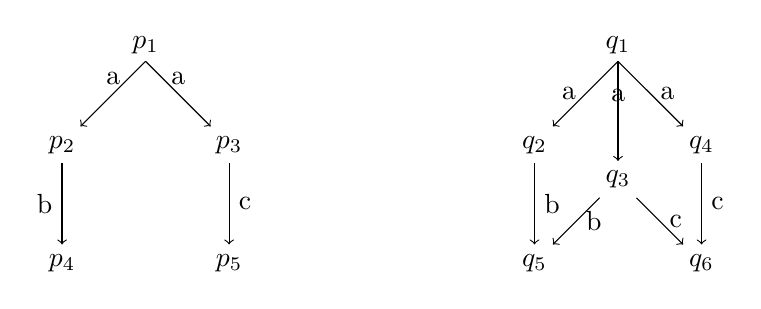
\begin{tikzpicture}[auto,node distance=1.5cm]
  \coordinate (p1) at (-3,0);
  \node at (-3, 0.2) {$p_1$}; 
  \node[below left of=p1] (p2) {$p_2$};
  \node[below right of=p1] (p3) {$p_3$};
  \node[below of=p2] (p4) {$p_4$};
  \node[below of=p3] (p5) {$p_5$};
  
  \draw[->] (p1) -- node[above] {a} (p2);
  \draw[->] (p1) -- node[above] {a} (p3);
  \draw[->] (p2) -- node[left] {b} (p4);
  \draw[->] (p3) -- node[right] {c} (p5);

\coordinate (q1) at (3,0);
  \node at (3, 0.2) {$q_1$}; 
  \node[below left of=q1] (q2) {$q_2$};
  \node[below of=q1] (q3) {$q_3$};
  \node[below right of=q1] (q4) {$q_4$};
  \node[below of=q2] (q5) {$q_5$};
  \node[below of=q4] (q6) {$q_6$};
  
  \draw[->] (q1) -- node[left] {a} (q2);
  \draw[->] (q1) -- node[above] {a} (q3);
  \draw[->] (q1) -- node[right] {a} (q4);
  \draw[->] (q2) -- node[right] {b} (q5);
  \draw[->] (q3) -- node[right] {b} (q5);
  \draw[->] (q3) -- node[right] {c} (q6);
  \draw[->] (q4) -- node[right] {c} (q6);
\end{tikzpicture}
\caption{TEEEEEEEEEEEEEEEEEEST}
    \label{fig:your_label}
\end{figure}%
\end{isamarkuptext}\isamarkuptrue%
\isacommand{definition}\isamarkupfalse%
\ expr{\isacharunderscore}{\kern0pt}ready{\isacharunderscore}{\kern0pt}trace\isanewline
\ \ \isakeyword{where}\isanewline
{\isachardoublequoteopen}expr{\isacharunderscore}{\kern0pt}ready{\isacharunderscore}{\kern0pt}trace\ {\isacharequal}{\kern0pt}\ {\isacharbraceleft}{\kern0pt}{\isasymphi}{\isachardot}{\kern0pt}\ {\isacharparenleft}{\kern0pt}less{\isacharunderscore}{\kern0pt}eq{\isacharunderscore}{\kern0pt}t\ {\isacharparenleft}{\kern0pt}expr\ {\isasymphi}{\isacharparenright}{\kern0pt}\ {\isacharparenleft}{\kern0pt}{\isasyminfinity}{\isacharcomma}{\kern0pt}\ {\isasyminfinity}{\isacharcomma}{\kern0pt}\ {\isasyminfinity}{\isacharcomma}{\kern0pt}\ {\isadigit{1}}{\isacharcomma}{\kern0pt}\ {\isadigit{1}}{\isacharcomma}{\kern0pt}\ {\isadigit{1}}{\isacharparenright}{\kern0pt}{\isacharparenright}{\kern0pt}{\isacharbraceright}{\kern0pt}{\isachardoublequoteclose}\isanewline
\isanewline
\isacommand{context}\isamarkupfalse%
\ lts\isanewline
\isakeyword{begin}\isanewline
\isanewline
\isacommand{definition}\isamarkupfalse%
\ expr{\isacharunderscore}{\kern0pt}ready{\isacharunderscore}{\kern0pt}trace{\isacharunderscore}{\kern0pt}equivalent\ \isanewline
\ \ \isakeyword{where}\isanewline
{\isachardoublequoteopen}expr{\isacharunderscore}{\kern0pt}ready{\isacharunderscore}{\kern0pt}trace{\isacharunderscore}{\kern0pt}equivalent\ p\ q\ {\isasymequiv}\ {\isacharparenleft}{\kern0pt}{\isasymforall}\ {\isasymphi}{\isachardot}{\kern0pt}\ {\isasymphi}\ {\isasymin}\ expr{\isacharunderscore}{\kern0pt}ready{\isacharunderscore}{\kern0pt}trace\ {\isasymlongrightarrow}\ {\isacharparenleft}{\kern0pt}p\ {\isasymTurnstile}\ {\isasymphi}{\isacharparenright}{\kern0pt}\ {\isasymlongleftrightarrow}\ {\isacharparenleft}{\kern0pt}q\ {\isasymTurnstile}\ {\isasymphi}{\isacharparenright}{\kern0pt}{\isacharparenright}{\kern0pt}{\isachardoublequoteclose}%
\begin{isamarkuptext}%
Proposition%
\end{isamarkuptext}\isamarkuptrue%
\isacommand{inductive}\isamarkupfalse%
\ HML{\isacharunderscore}{\kern0pt}readiness\ {\isacharcolon}{\kern0pt}{\isacharcolon}{\kern0pt}\ {\isachardoublequoteopen}{\isacharparenleft}{\kern0pt}{\isacharprime}{\kern0pt}a{\isacharcomma}{\kern0pt}\ {\isacharprime}{\kern0pt}s{\isacharparenright}{\kern0pt}hml\ {\isasymRightarrow}\ bool{\isachardoublequoteclose}\isanewline
\ \ \isakeyword{where}\isanewline
read{\isacharunderscore}{\kern0pt}tt{\isacharcolon}{\kern0pt}\ {\isachardoublequoteopen}HML{\isacharunderscore}{\kern0pt}readiness\ TT{\isachardoublequoteclose}\ {\isacharbar}{\kern0pt}\isanewline
read{\isacharunderscore}{\kern0pt}pos{\isacharcolon}{\kern0pt}\ {\isachardoublequoteopen}HML{\isacharunderscore}{\kern0pt}readiness\ {\isacharparenleft}{\kern0pt}hml{\isacharunderscore}{\kern0pt}pos\ {\isasymalpha}\ {\isasymphi}{\isacharparenright}{\kern0pt}{\isachardoublequoteclose}\ \isakeyword{if}\ {\isachardoublequoteopen}HML{\isacharunderscore}{\kern0pt}readiness\ {\isasymphi}{\isachardoublequoteclose}{\isacharbar}{\kern0pt}\isanewline
read{\isacharunderscore}{\kern0pt}conj{\isacharcolon}{\kern0pt}\ {\isachardoublequoteopen}HML{\isacharunderscore}{\kern0pt}readiness\ {\isacharparenleft}{\kern0pt}hml{\isacharunderscore}{\kern0pt}conj\ I\ J\ {\isasymPhi}{\isacharparenright}{\kern0pt}{\isachardoublequoteclose}\ \isanewline
\isakeyword{if}\ {\isachardoublequoteopen}{\isacharparenleft}{\kern0pt}{\isasymforall}x\ {\isasymin}\ {\isacharparenleft}{\kern0pt}{\isasymPhi}\ {\isacharbackquote}{\kern0pt}\ {\isacharparenleft}{\kern0pt}I\ {\isasymunion}\ J{\isacharparenright}{\kern0pt}{\isacharparenright}{\kern0pt}{\isachardot}{\kern0pt}\ TT{\isacharunderscore}{\kern0pt}like\ x\ {\isasymor}\ {\isacharparenleft}{\kern0pt}{\isasymexists}{\isasymalpha}\ {\isasymchi}{\isachardot}{\kern0pt}\ x\ {\isacharequal}{\kern0pt}\ hml{\isacharunderscore}{\kern0pt}pos\ {\isasymalpha}\ {\isasymchi}\ {\isasymand}\ TT{\isacharunderscore}{\kern0pt}like\ {\isasymchi}{\isacharparenright}{\kern0pt}{\isacharparenright}{\kern0pt}{\isachardoublequoteclose}\isanewline
\isanewline
\isanewline
\isacommand{lemma}\isamarkupfalse%
\ readiness{\isacharunderscore}{\kern0pt}right{\isacharcolon}{\kern0pt}\isanewline
\ \ \isakeyword{assumes}\ A{\isadigit{1}}{\isacharcolon}{\kern0pt}\ {\isachardoublequoteopen}HML{\isacharunderscore}{\kern0pt}readiness\ {\isasymphi}{\isachardoublequoteclose}\isanewline
\ \ \isakeyword{shows}\ {\isachardoublequoteopen}{\isacharparenleft}{\kern0pt}less{\isacharunderscore}{\kern0pt}eq{\isacharunderscore}{\kern0pt}t\ {\isacharparenleft}{\kern0pt}expr\ {\isasymphi}{\isacharparenright}{\kern0pt}\ {\isacharparenleft}{\kern0pt}{\isasyminfinity}{\isacharcomma}{\kern0pt}\ {\isadigit{2}}{\isacharcomma}{\kern0pt}\ {\isadigit{1}}{\isacharcomma}{\kern0pt}\ {\isadigit{1}}{\isacharcomma}{\kern0pt}\ {\isadigit{1}}{\isacharcomma}{\kern0pt}\ {\isadigit{1}}{\isacharparenright}{\kern0pt}{\isacharparenright}{\kern0pt}{\isachardoublequoteclose}\isanewline
%
\isadelimproof
\ \ %
\endisadelimproof
%
\isatagproof
\isacommand{using}\isamarkupfalse%
\ assms\isanewline
\isacommand{proof}\isamarkupfalse%
{\isacharparenleft}{\kern0pt}induction\ {\isasymphi}{\isacharparenright}{\kern0pt}\isanewline
\ \ \isacommand{case}\isamarkupfalse%
\ read{\isacharunderscore}{\kern0pt}tt\isanewline
\ \ \isacommand{then}\isamarkupfalse%
\ \isacommand{show}\isamarkupfalse%
\ {\isacharquery}{\kern0pt}case\ \isacommand{by}\isamarkupfalse%
\ simp\isanewline
\isacommand{next}\isamarkupfalse%
\isanewline
\ \ \isacommand{case}\isamarkupfalse%
\ {\isacharparenleft}{\kern0pt}read{\isacharunderscore}{\kern0pt}pos\ {\isasymphi}\ {\isasymalpha}{\isacharparenright}{\kern0pt}\isanewline
\ \ \isacommand{then}\isamarkupfalse%
\ \isacommand{show}\isamarkupfalse%
\ {\isacharquery}{\kern0pt}case\isanewline
\ \ \ \ \isacommand{by}\isamarkupfalse%
\ simp\isanewline
\isacommand{next}\isamarkupfalse%
\isanewline
\ \ \isacommand{case}\isamarkupfalse%
\ {\isacharparenleft}{\kern0pt}read{\isacharunderscore}{\kern0pt}conj\ {\isasymPhi}\ I\ J{\isacharparenright}{\kern0pt}\isanewline
\ \ \isacommand{from}\isamarkupfalse%
\ assms\ \isacommand{have}\isamarkupfalse%
\ {\isachardoublequoteopen}{\isacharparenleft}{\kern0pt}{\isasymforall}x\ {\isasymin}\ {\isacharparenleft}{\kern0pt}{\isasymPhi}\ {\isacharbackquote}{\kern0pt}\ I{\isacharparenright}{\kern0pt}\ {\isasymunion}\ {\isacharparenleft}{\kern0pt}{\isasymPhi}\ {\isacharbackquote}{\kern0pt}\ J{\isacharparenright}{\kern0pt}{\isachardot}{\kern0pt}\ TT{\isacharunderscore}{\kern0pt}like\ x\ {\isasymor}\ {\isacharparenleft}{\kern0pt}{\isasymexists}{\isasymalpha}\ {\isasymchi}{\isachardot}{\kern0pt}\ x\ {\isacharequal}{\kern0pt}\ hml{\isacharunderscore}{\kern0pt}pos\ {\isasymalpha}\ {\isasymchi}\ {\isasymand}\ TT{\isacharunderscore}{\kern0pt}like\ {\isasymchi}{\isacharparenright}{\kern0pt}{\isacharparenright}{\kern0pt}{\isachardoublequoteclose}\isanewline
\ \ \ \ \isacommand{using}\isamarkupfalse%
\ local{\isachardot}{\kern0pt}read{\isacharunderscore}{\kern0pt}conj\ \isacommand{by}\isamarkupfalse%
\ blast\isanewline
\ \ \isacommand{hence}\isamarkupfalse%
\ {\isachardoublequoteopen}{\isacharparenleft}{\kern0pt}{\isasymforall}x\ {\isasymin}\ {\isacharparenleft}{\kern0pt}{\isasymPhi}\ {\isacharbackquote}{\kern0pt}\ I{\isacharparenright}{\kern0pt}\ {\isasymunion}\ {\isacharparenleft}{\kern0pt}{\isasymPhi}\ {\isacharbackquote}{\kern0pt}\ J{\isacharparenright}{\kern0pt}{\isachardot}{\kern0pt}\ less{\isacharunderscore}{\kern0pt}eq{\isacharunderscore}{\kern0pt}t\ {\isacharparenleft}{\kern0pt}expr\ x{\isacharparenright}{\kern0pt}\ {\isacharparenleft}{\kern0pt}{\isadigit{1}}{\isacharcomma}{\kern0pt}\ {\isadigit{1}}{\isacharcomma}{\kern0pt}\ {\isadigit{0}}{\isacharcomma}{\kern0pt}\ {\isadigit{0}}{\isacharcomma}{\kern0pt}\ {\isadigit{0}}{\isacharcomma}{\kern0pt}\ {\isadigit{0}}{\isacharparenright}{\kern0pt}{\isacharparenright}{\kern0pt}{\isachardoublequoteclose}\isanewline
\ \ \ \ \isacommand{using}\isamarkupfalse%
\ e{\isadigit{1}}{\isacharunderscore}{\kern0pt}tt\ e{\isadigit{2}}{\isacharunderscore}{\kern0pt}tt\ e{\isadigit{3}}{\isacharunderscore}{\kern0pt}tt\ e{\isadigit{4}}{\isacharunderscore}{\kern0pt}tt\ e{\isadigit{5}}{\isacharunderscore}{\kern0pt}tt\ e{\isadigit{6}}{\isacharunderscore}{\kern0pt}tt\ expr{\isachardot}{\kern0pt}simps\ expr{\isacharunderscore}{\kern0pt}TT\isanewline
\ \ \ \ \isacommand{by}\isamarkupfalse%
\ {\isacharparenleft}{\kern0pt}metis\ dual{\isacharunderscore}{\kern0pt}order{\isachardot}{\kern0pt}refl\ i{\isadigit{0}}{\isacharunderscore}{\kern0pt}lb\ less{\isacharunderscore}{\kern0pt}eq{\isacharunderscore}{\kern0pt}t{\isachardot}{\kern0pt}simps{\isacharparenright}{\kern0pt}\isanewline
\ \ \isacommand{hence}\isamarkupfalse%
\ f{\isadigit{1}}{\isacharcolon}{\kern0pt}\ {\isachardoublequoteopen}{\isasymforall}x\ {\isasymin}\ {\isacharparenleft}{\kern0pt}{\isacharparenleft}{\kern0pt}expr{\isacharunderscore}{\kern0pt}{\isadigit{1}}\ {\isasymcirc}\ {\isasymPhi}{\isacharparenright}{\kern0pt}\ {\isacharbackquote}{\kern0pt}\ I{\isacharparenright}{\kern0pt}{\isachardot}{\kern0pt}\ x\ {\isasymle}\ {\isadigit{1}}{\isachardoublequoteclose}\isanewline
\ {\isachardoublequoteopen}{\isasymforall}x\ {\isasymin}\ {\isacharparenleft}{\kern0pt}{\isacharparenleft}{\kern0pt}expr{\isacharunderscore}{\kern0pt}{\isadigit{2}}\ {\isasymcirc}\ {\isasymPhi}{\isacharparenright}{\kern0pt}\ {\isacharbackquote}{\kern0pt}\ I{\isacharparenright}{\kern0pt}{\isachardot}{\kern0pt}\ x\ {\isasymle}\ {\isadigit{1}}{\isachardoublequoteclose}\isanewline
{\isachardoublequoteopen}{\isasymforall}x\ {\isasymin}\ {\isacharparenleft}{\kern0pt}{\isacharparenleft}{\kern0pt}expr{\isacharunderscore}{\kern0pt}{\isadigit{3}}\ {\isasymcirc}\ {\isasymPhi}{\isacharparenright}{\kern0pt}\ {\isacharbackquote}{\kern0pt}\ I{\isacharparenright}{\kern0pt}{\isachardot}{\kern0pt}\ x\ {\isasymle}\ {\isadigit{0}}{\isachardoublequoteclose}\isanewline
\ {\isachardoublequoteopen}{\isasymforall}x\ {\isasymin}\ {\isacharparenleft}{\kern0pt}{\isacharparenleft}{\kern0pt}expr{\isacharunderscore}{\kern0pt}{\isadigit{4}}\ {\isasymcirc}\ {\isasymPhi}{\isacharparenright}{\kern0pt}\ {\isacharbackquote}{\kern0pt}\ I{\isacharparenright}{\kern0pt}{\isachardot}{\kern0pt}\ x\ {\isasymle}\ {\isadigit{0}}{\isachardoublequoteclose}\isanewline
\ {\isachardoublequoteopen}{\isasymforall}x\ {\isasymin}\ {\isacharparenleft}{\kern0pt}{\isacharparenleft}{\kern0pt}expr{\isacharunderscore}{\kern0pt}{\isadigit{5}}\ {\isasymcirc}\ {\isasymPhi}{\isacharparenright}{\kern0pt}\ {\isacharbackquote}{\kern0pt}\ I{\isacharparenright}{\kern0pt}{\isachardot}{\kern0pt}\ x\ {\isasymle}\ {\isadigit{0}}{\isachardoublequoteclose}\isanewline
\ {\isachardoublequoteopen}{\isasymforall}x\ {\isasymin}\ {\isacharparenleft}{\kern0pt}{\isacharparenleft}{\kern0pt}expr{\isacharunderscore}{\kern0pt}{\isadigit{6}}\ {\isasymcirc}\ {\isasymPhi}{\isacharparenright}{\kern0pt}\ {\isacharbackquote}{\kern0pt}\ I{\isacharparenright}{\kern0pt}{\isachardot}{\kern0pt}\ x\ {\isasymle}\ \ {\isadigit{0}}{\isachardoublequoteclose}\isanewline
\isakeyword{and}\ f{\isadigit{2}}{\isacharcolon}{\kern0pt}\ {\isachardoublequoteopen}{\isasymforall}x\ {\isasymin}\ {\isacharparenleft}{\kern0pt}{\isacharparenleft}{\kern0pt}expr{\isacharunderscore}{\kern0pt}{\isadigit{1}}\ {\isasymcirc}\ {\isasymPhi}{\isacharparenright}{\kern0pt}\ {\isacharbackquote}{\kern0pt}\ J{\isacharparenright}{\kern0pt}{\isachardot}{\kern0pt}\ x\ {\isasymle}\ {\isadigit{1}}{\isachardoublequoteclose}\isanewline
\ {\isachardoublequoteopen}{\isasymforall}x\ {\isasymin}\ {\isacharparenleft}{\kern0pt}{\isacharparenleft}{\kern0pt}expr{\isacharunderscore}{\kern0pt}{\isadigit{2}}\ {\isasymcirc}\ {\isasymPhi}{\isacharparenright}{\kern0pt}\ {\isacharbackquote}{\kern0pt}\ J{\isacharparenright}{\kern0pt}{\isachardot}{\kern0pt}\ x\ {\isasymle}\ {\isadigit{1}}{\isachardoublequoteclose}\isanewline
{\isachardoublequoteopen}{\isasymforall}x\ {\isasymin}\ {\isacharparenleft}{\kern0pt}{\isacharparenleft}{\kern0pt}expr{\isacharunderscore}{\kern0pt}{\isadigit{3}}\ {\isasymcirc}\ {\isasymPhi}{\isacharparenright}{\kern0pt}\ {\isacharbackquote}{\kern0pt}\ J{\isacharparenright}{\kern0pt}{\isachardot}{\kern0pt}\ x\ {\isasymle}\ {\isadigit{0}}{\isachardoublequoteclose}\isanewline
\ {\isachardoublequoteopen}{\isasymforall}x\ {\isasymin}\ {\isacharparenleft}{\kern0pt}{\isacharparenleft}{\kern0pt}expr{\isacharunderscore}{\kern0pt}{\isadigit{4}}\ {\isasymcirc}\ {\isasymPhi}{\isacharparenright}{\kern0pt}\ {\isacharbackquote}{\kern0pt}\ J{\isacharparenright}{\kern0pt}{\isachardot}{\kern0pt}\ x\ {\isasymle}\ {\isadigit{0}}{\isachardoublequoteclose}\isanewline
\ {\isachardoublequoteopen}{\isasymforall}x\ {\isasymin}\ {\isacharparenleft}{\kern0pt}{\isacharparenleft}{\kern0pt}expr{\isacharunderscore}{\kern0pt}{\isadigit{5}}\ {\isasymcirc}\ {\isasymPhi}{\isacharparenright}{\kern0pt}\ {\isacharbackquote}{\kern0pt}\ J{\isacharparenright}{\kern0pt}{\isachardot}{\kern0pt}\ x\ {\isasymle}\ {\isadigit{0}}{\isachardoublequoteclose}\isanewline
\ {\isachardoublequoteopen}{\isasymforall}x\ {\isasymin}\ {\isacharparenleft}{\kern0pt}{\isacharparenleft}{\kern0pt}expr{\isacharunderscore}{\kern0pt}{\isadigit{6}}\ {\isasymcirc}\ {\isasymPhi}{\isacharparenright}{\kern0pt}\ {\isacharbackquote}{\kern0pt}\ J{\isacharparenright}{\kern0pt}{\isachardot}{\kern0pt}\ x\ {\isasymle}\ {\isadigit{0}}{\isachardoublequoteclose}\isanewline
\ \ \ \ \isacommand{using}\isamarkupfalse%
\ expr{\isachardot}{\kern0pt}simps\ \isanewline
\ \ \ \ \isacommand{by}\isamarkupfalse%
\ simp{\isacharplus}{\kern0pt}\isanewline
\isanewline
\ \ \isacommand{have}\isamarkupfalse%
\ {\isachardoublequoteopen}Sup\ {\isacharparenleft}{\kern0pt}{\isacharparenleft}{\kern0pt}expr{\isacharunderscore}{\kern0pt}{\isadigit{1}}\ {\isasymcirc}\ {\isasymPhi}{\isacharparenright}{\kern0pt}\ {\isacharbackquote}{\kern0pt}\ I{\isacharparenright}{\kern0pt}\ {\isasymle}\ {\isadigit{1}}{\isachardoublequoteclose}\isanewline
\isakeyword{and}\ {\isachardoublequoteopen}Sup\ {\isacharparenleft}{\kern0pt}{\isacharparenleft}{\kern0pt}expr{\isacharunderscore}{\kern0pt}{\isadigit{2}}\ {\isasymcirc}\ {\isasymPhi}{\isacharparenright}{\kern0pt}\ {\isacharbackquote}{\kern0pt}\ I{\isacharparenright}{\kern0pt}\ {\isasymle}\ {\isadigit{1}}{\isachardoublequoteclose}\isanewline
\isakeyword{and}\ {\isachardoublequoteopen}Sup\ {\isacharparenleft}{\kern0pt}{\isacharparenleft}{\kern0pt}expr{\isacharunderscore}{\kern0pt}{\isadigit{5}}\ {\isasymcirc}\ {\isasymPhi}{\isacharparenright}{\kern0pt}\ {\isacharbackquote}{\kern0pt}\ I{\isacharparenright}{\kern0pt}\ {\isasymle}\ {\isadigit{0}}{\isachardoublequoteclose}\isanewline
\isakeyword{and}\ {\isachardoublequoteopen}Sup\ {\isacharparenleft}{\kern0pt}{\isacharparenleft}{\kern0pt}expr{\isacharunderscore}{\kern0pt}{\isadigit{6}}\ {\isasymcirc}\ {\isasymPhi}{\isacharparenright}{\kern0pt}\ {\isacharbackquote}{\kern0pt}\ I{\isacharparenright}{\kern0pt}\ {\isasymle}\ {\isadigit{0}}{\isachardoublequoteclose}\isanewline
\isakeyword{and}\ {\isachardoublequoteopen}Sup\ {\isacharparenleft}{\kern0pt}{\isacharparenleft}{\kern0pt}expr{\isacharunderscore}{\kern0pt}{\isadigit{4}}\ {\isasymcirc}\ {\isasymPhi}{\isacharparenright}{\kern0pt}\ {\isacharbackquote}{\kern0pt}\ I{\isacharparenright}{\kern0pt}\ {\isasymle}\ {\isadigit{0}}{\isachardoublequoteclose}\isanewline
\isakeyword{and}\ {\isachardoublequoteopen}Sup\ {\isacharparenleft}{\kern0pt}{\isacharparenleft}{\kern0pt}expr{\isacharunderscore}{\kern0pt}{\isadigit{3}}\ {\isasymcirc}\ {\isasymPhi}{\isacharparenright}{\kern0pt}\ {\isacharbackquote}{\kern0pt}\ I{\isacharparenright}{\kern0pt}\ {\isasymle}\ {\isadigit{0}}{\isachardoublequoteclose}\isanewline
\ \ \ \ \isacommand{using}\isamarkupfalse%
\ Sup{\isacharunderscore}{\kern0pt}le{\isacharunderscore}{\kern0pt}iff\ f{\isadigit{1}}\isanewline
\ \ \ \ \ \ \ \ \ \isacommand{apply}\isamarkupfalse%
\ {\isacharparenleft}{\kern0pt}simp\ add{\isacharcolon}{\kern0pt}\ SUP{\isacharunderscore}{\kern0pt}least{\isacharparenright}{\kern0pt}\isanewline
\ \ \ \ \isacommand{using}\isamarkupfalse%
\ Sup{\isacharunderscore}{\kern0pt}le{\isacharunderscore}{\kern0pt}iff\ f{\isadigit{1}}\isanewline
\ \ \ \ \ \ \ \ \ \isacommand{apply}\isamarkupfalse%
\ {\isacharparenleft}{\kern0pt}simp\ add{\isacharcolon}{\kern0pt}\ SUP{\isacharunderscore}{\kern0pt}least{\isacharparenright}{\kern0pt}\isanewline
\ \ \ \ \isacommand{using}\isamarkupfalse%
\ Sup{\isacharunderscore}{\kern0pt}le{\isacharunderscore}{\kern0pt}iff\ f{\isadigit{1}}\isanewline
\ \ \ \ \isacommand{by}\isamarkupfalse%
\ {\isacharparenleft}{\kern0pt}metis{\isacharparenright}{\kern0pt}{\isacharplus}{\kern0pt}\isanewline
\isanewline
\ \ \isacommand{have}\isamarkupfalse%
\ {\isachardoublequoteopen}Sup\ {\isacharparenleft}{\kern0pt}{\isacharparenleft}{\kern0pt}expr{\isacharunderscore}{\kern0pt}{\isadigit{1}}\ {\isasymcirc}\ {\isasymPhi}{\isacharparenright}{\kern0pt}\ {\isacharbackquote}{\kern0pt}\ J{\isacharparenright}{\kern0pt}\ {\isasymle}\ {\isadigit{1}}{\isachardoublequoteclose}\isanewline
\isakeyword{and}\ {\isachardoublequoteopen}Sup\ {\isacharparenleft}{\kern0pt}{\isacharparenleft}{\kern0pt}expr{\isacharunderscore}{\kern0pt}{\isadigit{2}}\ {\isasymcirc}\ {\isasymPhi}{\isacharparenright}{\kern0pt}\ {\isacharbackquote}{\kern0pt}\ J{\isacharparenright}{\kern0pt}\ {\isasymle}\ {\isadigit{1}}{\isachardoublequoteclose}\isanewline
\isakeyword{and}\ {\isachardoublequoteopen}Sup\ {\isacharparenleft}{\kern0pt}{\isacharparenleft}{\kern0pt}expr{\isacharunderscore}{\kern0pt}{\isadigit{5}}\ {\isasymcirc}\ {\isasymPhi}{\isacharparenright}{\kern0pt}\ {\isacharbackquote}{\kern0pt}\ J{\isacharparenright}{\kern0pt}\ {\isasymle}\ {\isadigit{0}}{\isachardoublequoteclose}\isanewline
\isakeyword{and}\ {\isachardoublequoteopen}Sup\ {\isacharparenleft}{\kern0pt}{\isacharparenleft}{\kern0pt}expr{\isacharunderscore}{\kern0pt}{\isadigit{6}}\ {\isasymcirc}\ {\isasymPhi}{\isacharparenright}{\kern0pt}\ {\isacharbackquote}{\kern0pt}\ J{\isacharparenright}{\kern0pt}\ {\isasymle}\ {\isadigit{0}}{\isachardoublequoteclose}\isanewline
\isakeyword{and}\ {\isachardoublequoteopen}Sup\ {\isacharparenleft}{\kern0pt}{\isacharparenleft}{\kern0pt}expr{\isacharunderscore}{\kern0pt}{\isadigit{4}}\ {\isasymcirc}\ {\isasymPhi}{\isacharparenright}{\kern0pt}\ {\isacharbackquote}{\kern0pt}\ J{\isacharparenright}{\kern0pt}\ {\isasymle}\ {\isadigit{0}}{\isachardoublequoteclose}\isanewline
\isakeyword{and}\ {\isachardoublequoteopen}Sup\ {\isacharparenleft}{\kern0pt}{\isacharparenleft}{\kern0pt}expr{\isacharunderscore}{\kern0pt}{\isadigit{3}}\ {\isasymcirc}\ {\isasymPhi}{\isacharparenright}{\kern0pt}\ {\isacharbackquote}{\kern0pt}\ J{\isacharparenright}{\kern0pt}\ {\isasymle}\ {\isadigit{0}}{\isachardoublequoteclose}\ \isanewline
\isacommand{using}\isamarkupfalse%
\ Sup{\isacharunderscore}{\kern0pt}le{\isacharunderscore}{\kern0pt}iff\ f{\isadigit{2}}\isanewline
\ \ \ \ \ \ \ \ \ \isacommand{apply}\isamarkupfalse%
\ {\isacharparenleft}{\kern0pt}simp\ add{\isacharcolon}{\kern0pt}\ SUP{\isacharunderscore}{\kern0pt}least{\isacharparenright}{\kern0pt}\isanewline
\ \ \ \ \isacommand{using}\isamarkupfalse%
\ Sup{\isacharunderscore}{\kern0pt}le{\isacharunderscore}{\kern0pt}iff\ f{\isadigit{2}}\isanewline
\ \ \ \ \ \ \ \ \ \isacommand{apply}\isamarkupfalse%
\ {\isacharparenleft}{\kern0pt}simp\ add{\isacharcolon}{\kern0pt}\ SUP{\isacharunderscore}{\kern0pt}least{\isacharparenright}{\kern0pt}\isanewline
\ \ \ \ \isacommand{using}\isamarkupfalse%
\ Sup{\isacharunderscore}{\kern0pt}le{\isacharunderscore}{\kern0pt}iff\ f{\isadigit{2}}\isanewline
\ \ \ \ \isacommand{by}\isamarkupfalse%
\ {\isacharparenleft}{\kern0pt}metis{\isacharparenright}{\kern0pt}{\isacharplus}{\kern0pt}\isanewline
\isanewline
\ \ \isacommand{have}\isamarkupfalse%
\ e{\isadigit{2}}{\isacharcolon}{\kern0pt}\ {\isachardoublequoteopen}expr{\isacharunderscore}{\kern0pt}{\isadigit{2}}\ {\isacharparenleft}{\kern0pt}hml{\isacharunderscore}{\kern0pt}conj\ I\ J\ {\isasymPhi}{\isacharparenright}{\kern0pt}\ {\isasymle}\ {\isadigit{2}}{\isachardoublequoteclose}\isanewline
\ \ \ \ \isacommand{using}\isamarkupfalse%
\ {\isacartoucheopen}Sup\ {\isacharparenleft}{\kern0pt}{\isacharparenleft}{\kern0pt}expr{\isacharunderscore}{\kern0pt}{\isadigit{2}}\ {\isasymcirc}\ {\isasymPhi}{\isacharparenright}{\kern0pt}\ {\isacharbackquote}{\kern0pt}\ I{\isacharparenright}{\kern0pt}\ {\isasymle}\ {\isadigit{1}}{\isacartoucheclose}\ {\isacartoucheopen}Sup\ {\isacharparenleft}{\kern0pt}{\isacharparenleft}{\kern0pt}expr{\isacharunderscore}{\kern0pt}{\isadigit{2}}\ {\isasymcirc}\ {\isasymPhi}{\isacharparenright}{\kern0pt}\ {\isacharbackquote}{\kern0pt}\ J{\isacharparenright}{\kern0pt}\ {\isasymle}\ {\isadigit{1}}{\isacartoucheclose}\ expr{\isacharunderscore}{\kern0pt}{\isadigit{2}}{\isacharunderscore}{\kern0pt}conj\ one{\isacharunderscore}{\kern0pt}add{\isacharunderscore}{\kern0pt}one\isanewline
\ \ \ \ \isacommand{by}\isamarkupfalse%
\ {\isacharparenleft}{\kern0pt}metis\ Sup{\isacharunderscore}{\kern0pt}union{\isacharunderscore}{\kern0pt}distrib\ add{\isacharunderscore}{\kern0pt}left{\isacharunderscore}{\kern0pt}mono\ le{\isacharunderscore}{\kern0pt}sup{\isacharunderscore}{\kern0pt}iff{\isacharparenright}{\kern0pt}\isanewline
\ \ \isacommand{have}\isamarkupfalse%
\ e{\isadigit{3}}{\isacharcolon}{\kern0pt}\ {\isachardoublequoteopen}expr{\isacharunderscore}{\kern0pt}{\isadigit{3}}\ {\isacharparenleft}{\kern0pt}hml{\isacharunderscore}{\kern0pt}conj\ I\ J\ {\isasymPhi}{\isacharparenright}{\kern0pt}\ {\isasymle}\ {\isadigit{1}}{\isachardoublequoteclose}\isanewline
\ \ \ \ \isacommand{using}\isamarkupfalse%
\ {\isacartoucheopen}Sup\ {\isacharparenleft}{\kern0pt}{\isacharparenleft}{\kern0pt}expr{\isacharunderscore}{\kern0pt}{\isadigit{1}}\ {\isasymcirc}\ {\isasymPhi}{\isacharparenright}{\kern0pt}\ {\isacharbackquote}{\kern0pt}\ I{\isacharparenright}{\kern0pt}\ {\isasymle}\ {\isadigit{1}}{\isacartoucheclose}\ {\isacartoucheopen}Sup\ {\isacharparenleft}{\kern0pt}{\isacharparenleft}{\kern0pt}expr{\isacharunderscore}{\kern0pt}{\isadigit{3}}\ {\isasymcirc}\ {\isasymPhi}{\isacharparenright}{\kern0pt}\ {\isacharbackquote}{\kern0pt}\ J{\isacharparenright}{\kern0pt}\ {\isasymle}\ {\isadigit{0}}{\isacartoucheclose}\ {\isacartoucheopen}Sup\ {\isacharparenleft}{\kern0pt}{\isacharparenleft}{\kern0pt}expr{\isacharunderscore}{\kern0pt}{\isadigit{3}}\ {\isasymcirc}\ {\isasymPhi}{\isacharparenright}{\kern0pt}\ {\isacharbackquote}{\kern0pt}\ I{\isacharparenright}{\kern0pt}\ {\isasymle}\ {\isadigit{0}}{\isacartoucheclose}\ \isanewline
one{\isacharunderscore}{\kern0pt}add{\isacharunderscore}{\kern0pt}one\ expr{\isacharunderscore}{\kern0pt}{\isadigit{3}}{\isacharunderscore}{\kern0pt}conj\ Sup{\isacharunderscore}{\kern0pt}union{\isacharunderscore}{\kern0pt}distrib\ add{\isacharunderscore}{\kern0pt}left{\isacharunderscore}{\kern0pt}mono\ le{\isacharunderscore}{\kern0pt}sup{\isacharunderscore}{\kern0pt}iff\isanewline
\ \ \ \ \isacommand{by}\isamarkupfalse%
\ {\isacharparenleft}{\kern0pt}smt\ {\isacharparenleft}{\kern0pt}verit{\isacharparenright}{\kern0pt}\ le{\isacharunderscore}{\kern0pt}zero{\isacharunderscore}{\kern0pt}eq\ max{\isacharunderscore}{\kern0pt}def\ sup{\isacharunderscore}{\kern0pt}enat{\isacharunderscore}{\kern0pt}def{\isacharparenright}{\kern0pt}\isanewline
\ \ \isacommand{from}\isamarkupfalse%
\ {\isacartoucheopen}Sup\ {\isacharparenleft}{\kern0pt}{\isacharparenleft}{\kern0pt}expr{\isacharunderscore}{\kern0pt}{\isadigit{1}}\ {\isasymcirc}\ {\isasymPhi}{\isacharparenright}{\kern0pt}\ {\isacharbackquote}{\kern0pt}\ I{\isacharparenright}{\kern0pt}\ {\isasymle}\ {\isadigit{1}}{\isacartoucheclose}\ \isacommand{have}\isamarkupfalse%
\ {\isachardoublequoteopen}Sup\ {\isacharparenleft}{\kern0pt}expr{\isacharunderscore}{\kern0pt}{\isadigit{1}}\ {\isacharbackquote}{\kern0pt}\ {\isacharparenleft}{\kern0pt}pos{\isacharunderscore}{\kern0pt}r\ {\isacharparenleft}{\kern0pt}{\isasymPhi}\ {\isacharbackquote}{\kern0pt}\ I{\isacharparenright}{\kern0pt}{\isacharparenright}{\kern0pt}{\isacharparenright}{\kern0pt}\ {\isacharless}{\kern0pt}{\isacharequal}{\kern0pt}\ {\isadigit{1}}{\isachardoublequoteclose}\ \isanewline
\ \ \ \ \isacommand{using}\isamarkupfalse%
\ SUP{\isacharunderscore}{\kern0pt}image\ dual{\isacharunderscore}{\kern0pt}order{\isachardot}{\kern0pt}trans\ mon{\isacharunderscore}{\kern0pt}expr{\isacharunderscore}{\kern0pt}{\isadigit{1}}{\isacharunderscore}{\kern0pt}pos{\isacharunderscore}{\kern0pt}r\ \isanewline
\ \ \ \ \isacommand{by}\isamarkupfalse%
\ metis\ \isanewline
\ \ \isacommand{hence}\isamarkupfalse%
\ e{\isadigit{4}}{\isacharcolon}{\kern0pt}\ {\isachardoublequoteopen}expr{\isacharunderscore}{\kern0pt}{\isadigit{4}}\ {\isacharparenleft}{\kern0pt}hml{\isacharunderscore}{\kern0pt}conj\ I\ J\ {\isasymPhi}{\isacharparenright}{\kern0pt}\ {\isasymle}\ {\isadigit{1}}{\isachardoublequoteclose}\ \isanewline
\ \ \ \ \isacommand{using}\isamarkupfalse%
\ {\isacartoucheopen}Sup\ {\isacharparenleft}{\kern0pt}{\isacharparenleft}{\kern0pt}expr{\isacharunderscore}{\kern0pt}{\isadigit{4}}\ {\isasymcirc}\ {\isasymPhi}{\isacharparenright}{\kern0pt}\ {\isacharbackquote}{\kern0pt}\ I{\isacharparenright}{\kern0pt}\ {\isasymle}\ {\isadigit{0}}{\isacartoucheclose}\ {\isacartoucheopen}Sup\ {\isacharparenleft}{\kern0pt}{\isacharparenleft}{\kern0pt}expr{\isacharunderscore}{\kern0pt}{\isadigit{4}}\ {\isasymcirc}\ {\isasymPhi}{\isacharparenright}{\kern0pt}\ {\isacharbackquote}{\kern0pt}\ J{\isacharparenright}{\kern0pt}\ {\isasymle}\ {\isadigit{0}}{\isacartoucheclose}\isanewline
one{\isacharunderscore}{\kern0pt}add{\isacharunderscore}{\kern0pt}one\ expr{\isacharunderscore}{\kern0pt}{\isadigit{4}}{\isacharunderscore}{\kern0pt}conj\ Sup{\isacharunderscore}{\kern0pt}union{\isacharunderscore}{\kern0pt}distrib\ add{\isacharunderscore}{\kern0pt}left{\isacharunderscore}{\kern0pt}mono\ le{\isacharunderscore}{\kern0pt}sup{\isacharunderscore}{\kern0pt}iff\isanewline
\ \ \ \ \isacommand{by}\isamarkupfalse%
\ {\isacharparenleft}{\kern0pt}smt\ {\isacharparenleft}{\kern0pt}verit{\isacharparenright}{\kern0pt}\ le{\isacharunderscore}{\kern0pt}zero{\isacharunderscore}{\kern0pt}eq\ max{\isacharunderscore}{\kern0pt}def\ sup{\isacharunderscore}{\kern0pt}enat{\isacharunderscore}{\kern0pt}def{\isacharparenright}{\kern0pt}\isanewline
\ \ \isacommand{have}\isamarkupfalse%
\ e{\isadigit{5}}{\isacharcolon}{\kern0pt}\ {\isachardoublequoteopen}expr{\isacharunderscore}{\kern0pt}{\isadigit{5}}\ {\isacharparenleft}{\kern0pt}hml{\isacharunderscore}{\kern0pt}conj\ I\ J\ {\isasymPhi}{\isacharparenright}{\kern0pt}\ {\isasymle}\ {\isadigit{1}}{\isachardoublequoteclose}\ \isanewline
\ \ \ \ \isacommand{using}\isamarkupfalse%
\ {\isacartoucheopen}Sup\ {\isacharparenleft}{\kern0pt}{\isacharparenleft}{\kern0pt}expr{\isacharunderscore}{\kern0pt}{\isadigit{5}}\ {\isasymcirc}\ {\isasymPhi}{\isacharparenright}{\kern0pt}\ {\isacharbackquote}{\kern0pt}\ I{\isacharparenright}{\kern0pt}\ {\isasymle}\ {\isadigit{0}}{\isacartoucheclose}\ {\isacartoucheopen}Sup\ {\isacharparenleft}{\kern0pt}{\isacharparenleft}{\kern0pt}expr{\isacharunderscore}{\kern0pt}{\isadigit{5}}\ {\isasymcirc}\ {\isasymPhi}{\isacharparenright}{\kern0pt}\ {\isacharbackquote}{\kern0pt}\ J{\isacharparenright}{\kern0pt}\ {\isasymle}\ {\isadigit{0}}{\isacartoucheclose}\ {\isacartoucheopen}Sup\ {\isacharparenleft}{\kern0pt}{\isacharparenleft}{\kern0pt}expr{\isacharunderscore}{\kern0pt}{\isadigit{1}}\ {\isasymcirc}\ {\isasymPhi}{\isacharparenright}{\kern0pt}\ {\isacharbackquote}{\kern0pt}\ J{\isacharparenright}{\kern0pt}\ {\isasymle}\ {\isadigit{1}}{\isacartoucheclose}\ expr{\isacharunderscore}{\kern0pt}{\isadigit{5}}{\isacharunderscore}{\kern0pt}conj\ \isanewline
\ \ \ \ \isacommand{by}\isamarkupfalse%
\ {\isacharparenleft}{\kern0pt}simp\ add{\isacharcolon}{\kern0pt}\ Sup{\isacharunderscore}{\kern0pt}union{\isacharunderscore}{\kern0pt}distrib{\isacharparenright}{\kern0pt}\isanewline
\ \ \isacommand{from}\isamarkupfalse%
\ {\isacartoucheopen}Sup\ {\isacharparenleft}{\kern0pt}{\isacharparenleft}{\kern0pt}expr{\isacharunderscore}{\kern0pt}{\isadigit{6}}\ {\isasymcirc}\ {\isasymPhi}{\isacharparenright}{\kern0pt}\ {\isacharbackquote}{\kern0pt}\ J{\isacharparenright}{\kern0pt}\ {\isasymle}\ {\isadigit{0}}{\isacartoucheclose}\ \isacommand{have}\isamarkupfalse%
\ {\isachardoublequoteopen}Sup\ {\isacharparenleft}{\kern0pt}{\isacharparenleft}{\kern0pt}eSuc\ {\isasymcirc}\ expr{\isacharunderscore}{\kern0pt}{\isadigit{6}}\ {\isasymcirc}\ {\isasymPhi}{\isacharparenright}{\kern0pt}\ {\isacharbackquote}{\kern0pt}\ J{\isacharparenright}{\kern0pt}\ {\isasymle}\ {\isadigit{1}}{\isachardoublequoteclose}\isanewline
\ \ \ \ \isacommand{using}\isamarkupfalse%
\ eSuc{\isacharunderscore}{\kern0pt}def\ f{\isadigit{2}}{\isacharparenleft}{\kern0pt}{\isadigit{6}}{\isacharparenright}{\kern0pt}\isanewline
\ \ \ \ \isacommand{by}\isamarkupfalse%
\ {\isacharparenleft}{\kern0pt}metis\ eSuc{\isacharunderscore}{\kern0pt}Sup\ image{\isacharunderscore}{\kern0pt}comp\ image{\isacharunderscore}{\kern0pt}is{\isacharunderscore}{\kern0pt}empty\ nle{\isacharunderscore}{\kern0pt}le\ one{\isacharunderscore}{\kern0pt}eSuc\ zero{\isacharunderscore}{\kern0pt}le{\isacharparenright}{\kern0pt}\ \isanewline
\ \ \ \ \isacommand{hence}\isamarkupfalse%
\ e{\isadigit{6}}{\isacharcolon}{\kern0pt}\ {\isachardoublequoteopen}expr{\isacharunderscore}{\kern0pt}{\isadigit{6}}\ {\isacharparenleft}{\kern0pt}hml{\isacharunderscore}{\kern0pt}conj\ I\ J\ {\isasymPhi}{\isacharparenright}{\kern0pt}\ {\isasymle}\ {\isadigit{1}}{\isachardoublequoteclose}\isanewline
\ \ \ \ \isacommand{using}\isamarkupfalse%
\ {\isacartoucheopen}Sup\ {\isacharparenleft}{\kern0pt}{\isacharparenleft}{\kern0pt}expr{\isacharunderscore}{\kern0pt}{\isadigit{6}}\ {\isasymcirc}\ {\isasymPhi}{\isacharparenright}{\kern0pt}\ {\isacharbackquote}{\kern0pt}\ I{\isacharparenright}{\kern0pt}\ {\isasymle}\ {\isadigit{0}}{\isacartoucheclose}\ expr{\isacharunderscore}{\kern0pt}{\isadigit{6}}{\isacharunderscore}{\kern0pt}conj\ \isanewline
\ \ \ \ \isacommand{by}\isamarkupfalse%
\ {\isacharparenleft}{\kern0pt}simp\ add{\isacharcolon}{\kern0pt}\ Sup{\isacharunderscore}{\kern0pt}union{\isacharunderscore}{\kern0pt}distrib{\isacharparenright}{\kern0pt}\isanewline
\ \ \isacommand{from}\isamarkupfalse%
\ e{\isadigit{2}}\ e{\isadigit{3}}\ e{\isadigit{4}}\ e{\isadigit{5}}\ e{\isadigit{6}}\ \isacommand{show}\isamarkupfalse%
\ {\isacharquery}{\kern0pt}case\ \isacommand{using}\isamarkupfalse%
\ less{\isacharunderscore}{\kern0pt}eq{\isacharunderscore}{\kern0pt}t{\isachardot}{\kern0pt}simps\ expr{\isachardot}{\kern0pt}simps\ \isanewline
\ \ \ \ \isacommand{by}\isamarkupfalse%
\ {\isacharparenleft}{\kern0pt}metis\ enat{\isacharunderscore}{\kern0pt}ord{\isacharunderscore}{\kern0pt}code{\isacharparenleft}{\kern0pt}{\isadigit{3}}{\isacharparenright}{\kern0pt}{\isacharparenright}{\kern0pt}\isanewline
\isacommand{qed}\isamarkupfalse%
%
\endisatagproof
{\isafoldproof}%
%
\isadelimproof
\isanewline
%
\endisadelimproof
\isanewline
\isacommand{lemma}\isamarkupfalse%
\ expr{\isacharunderscore}{\kern0pt}{\isadigit{2}}{\isacharunderscore}{\kern0pt}expr{\isacharunderscore}{\kern0pt}{\isadigit{3}}{\isacharunderscore}{\kern0pt}restrict{\isacharunderscore}{\kern0pt}positives{\isacharcolon}{\kern0pt}\isanewline
\ \ \isakeyword{assumes}\ {\isachardoublequoteopen}{\isacharparenleft}{\kern0pt}expr{\isacharunderscore}{\kern0pt}{\isadigit{2}}\ {\isacharparenleft}{\kern0pt}hml{\isacharunderscore}{\kern0pt}conj\ I\ J\ {\isasymPhi}{\isacharparenright}{\kern0pt}{\isacharparenright}{\kern0pt}\ {\isasymle}\ {\isadigit{2}}{\isachardoublequoteclose}\ {\isachardoublequoteopen}{\isacharparenleft}{\kern0pt}expr{\isacharunderscore}{\kern0pt}{\isadigit{3}}\ {\isacharparenleft}{\kern0pt}hml{\isacharunderscore}{\kern0pt}conj\ I\ J\ {\isasymPhi}{\isacharparenright}{\kern0pt}{\isacharparenright}{\kern0pt}\ {\isasymle}\ {\isadigit{1}}{\isachardoublequoteclose}\isanewline
\ \ \isakeyword{shows}\ {\isachardoublequoteopen}{\isacharparenleft}{\kern0pt}{\isasymforall}x\ {\isasymin}\ {\isacharparenleft}{\kern0pt}{\isasymPhi}\ {\isacharbackquote}{\kern0pt}\ I{\isacharparenright}{\kern0pt}{\isachardot}{\kern0pt}\ TT{\isacharunderscore}{\kern0pt}like\ x\ {\isasymor}\ {\isacharparenleft}{\kern0pt}{\isasymexists}{\isasymalpha}\ {\isasymchi}{\isachardot}{\kern0pt}\ x\ {\isacharequal}{\kern0pt}\ hml{\isacharunderscore}{\kern0pt}pos\ {\isasymalpha}\ {\isasymchi}\ {\isasymand}\ TT{\isacharunderscore}{\kern0pt}like\ {\isasymchi}{\isacharparenright}{\kern0pt}{\isacharparenright}{\kern0pt}{\isachardoublequoteclose}\isanewline
%
\isadelimproof
%
\endisadelimproof
%
\isatagproof
\isacommand{proof}\isamarkupfalse%
\isanewline
\ \ \isacommand{fix}\isamarkupfalse%
\ x\isanewline
\ \ \isacommand{assume}\isamarkupfalse%
\ {\isachardoublequoteopen}x\ {\isasymin}\ {\isasymPhi}\ {\isacharbackquote}{\kern0pt}\ I{\isachardoublequoteclose}\isanewline
\ \ \isacommand{hence}\isamarkupfalse%
\ {\isachardoublequoteopen}expr{\isacharunderscore}{\kern0pt}{\isadigit{2}}\ x\ {\isasymle}\ Sup\ {\isacharparenleft}{\kern0pt}expr{\isacharunderscore}{\kern0pt}{\isadigit{2}}\ {\isacharbackquote}{\kern0pt}\ {\isasymPhi}\ {\isacharbackquote}{\kern0pt}\ I{\isacharparenright}{\kern0pt}{\isachardoublequoteclose}\isanewline
\ \ \ \ \isacommand{by}\isamarkupfalse%
\ {\isacharparenleft}{\kern0pt}simp\ add{\isacharcolon}{\kern0pt}\ Sup{\isacharunderscore}{\kern0pt}upper{\isacharparenright}{\kern0pt}\isanewline
\isacommand{hence}\isamarkupfalse%
\ {\isachardoublequoteopen}expr{\isacharunderscore}{\kern0pt}{\isadigit{2}}\ x\ {\isasymle}\ Sup\ {\isacharparenleft}{\kern0pt}{\isacharparenleft}{\kern0pt}expr{\isacharunderscore}{\kern0pt}{\isadigit{2}}\ {\isasymcirc}\ {\isasymPhi}{\isacharparenright}{\kern0pt}\ {\isacharbackquote}{\kern0pt}\ I{\isacharparenright}{\kern0pt}{\isachardoublequoteclose}\isanewline
\ \ \isacommand{by}\isamarkupfalse%
\ {\isacharparenleft}{\kern0pt}simp\ add{\isacharcolon}{\kern0pt}\ SUP{\isacharunderscore}{\kern0pt}image{\isacharparenright}{\kern0pt}\isanewline
\ \ \isacommand{hence}\isamarkupfalse%
\ {\isachardoublequoteopen}expr{\isacharunderscore}{\kern0pt}{\isadigit{2}}\ x\ {\isasymle}\ Sup\ {\isacharparenleft}{\kern0pt}{\isacharparenleft}{\kern0pt}expr{\isacharunderscore}{\kern0pt}{\isadigit{2}}\ {\isasymcirc}\ {\isasymPhi}{\isacharparenright}{\kern0pt}\ {\isacharbackquote}{\kern0pt}\ I\ {\isasymunion}\ {\isacharparenleft}{\kern0pt}expr{\isacharunderscore}{\kern0pt}{\isadigit{2}}\ {\isasymcirc}\ {\isasymPhi}{\isacharparenright}{\kern0pt}\ {\isacharbackquote}{\kern0pt}\ J{\isacharparenright}{\kern0pt}{\isachardoublequoteclose}\isanewline
\ \ \ \ \isacommand{by}\isamarkupfalse%
\ {\isacharparenleft}{\kern0pt}simp\ add{\isacharcolon}{\kern0pt}\ Sup{\isacharunderscore}{\kern0pt}union{\isacharunderscore}{\kern0pt}distrib\ sup{\isachardot}{\kern0pt}coboundedI{\isadigit{1}}{\isacharparenright}{\kern0pt}\isanewline
\ \ \isacommand{hence}\isamarkupfalse%
\ {\isachardoublequoteopen}expr{\isacharunderscore}{\kern0pt}{\isadigit{2}}\ x\ {\isasymle}\ {\isadigit{1}}{\isachardoublequoteclose}\ \isacommand{using}\isamarkupfalse%
\ assms{\isacharparenleft}{\kern0pt}{\isadigit{1}}{\isacharparenright}{\kern0pt}\ expr{\isacharunderscore}{\kern0pt}{\isadigit{2}}{\isacharunderscore}{\kern0pt}conj\ one{\isacharunderscore}{\kern0pt}add{\isacharunderscore}{\kern0pt}one\isanewline
\ \ \ \ \isacommand{by}\isamarkupfalse%
\ {\isacharparenleft}{\kern0pt}metis\ enat{\isacharunderscore}{\kern0pt}add{\isacharunderscore}{\kern0pt}left{\isacharunderscore}{\kern0pt}cancel{\isacharunderscore}{\kern0pt}le\ expr{\isacharunderscore}{\kern0pt}{\isadigit{2}}{\isacharunderscore}{\kern0pt}lb\ le{\isacharunderscore}{\kern0pt}iff{\isacharunderscore}{\kern0pt}add\ le{\isacharunderscore}{\kern0pt}sup{\isacharunderscore}{\kern0pt}iff\ plus{\isacharunderscore}{\kern0pt}{\isadigit{1}}{\isacharunderscore}{\kern0pt}eSuc{\isacharparenleft}{\kern0pt}{\isadigit{1}}{\isacharparenright}{\kern0pt}\ sup{\isachardot}{\kern0pt}orderE{\isacharparenright}{\kern0pt}\isanewline
\ \ \isacommand{show}\isamarkupfalse%
\ {\isachardoublequoteopen}TT{\isacharunderscore}{\kern0pt}like\ x\ {\isasymor}\ {\isacharparenleft}{\kern0pt}{\isasymexists}{\isasymalpha}\ {\isasymchi}{\isachardot}{\kern0pt}\ x\ {\isacharequal}{\kern0pt}\ hml{\isacharunderscore}{\kern0pt}pos\ {\isasymalpha}\ {\isasymchi}\ {\isasymand}\ TT{\isacharunderscore}{\kern0pt}like\ {\isasymchi}{\isacharparenright}{\kern0pt}{\isachardoublequoteclose}\isanewline
\ \ \isacommand{proof}\isamarkupfalse%
{\isacharparenleft}{\kern0pt}cases\ x{\isacharparenright}{\kern0pt}\isanewline
\ \ \ \ \isacommand{case}\isamarkupfalse%
\ TT\isanewline
\ \ \ \ \isacommand{then}\isamarkupfalse%
\ \isacommand{show}\isamarkupfalse%
\ {\isacharquery}{\kern0pt}thesis\ \isacommand{using}\isamarkupfalse%
\ TT{\isacharunderscore}{\kern0pt}like{\isachardot}{\kern0pt}simps\isanewline
\ \ \ \ \ \ \isacommand{by}\isamarkupfalse%
\ blast\isanewline
\ \ \isacommand{next}\isamarkupfalse%
\isanewline
\ \ \ \ \isacommand{case}\isamarkupfalse%
\ {\isacharparenleft}{\kern0pt}hml{\isacharunderscore}{\kern0pt}pos\ {\isasymalpha}\ {\isasympsi}{\isacharparenright}{\kern0pt}\isanewline
\ \ \ \ \isacommand{have}\isamarkupfalse%
\ {\isachardoublequoteopen}TT{\isacharunderscore}{\kern0pt}like\ {\isasympsi}{\isachardoublequoteclose}\isanewline
\ \ \ \ \isacommand{proof}\isamarkupfalse%
{\isacharparenleft}{\kern0pt}cases\ {\isasympsi}{\isacharparenright}{\kern0pt}\isanewline
\ \ \ \ \ \ \isacommand{case}\isamarkupfalse%
\ TT\isanewline
\ \ \ \ \ \ \isacommand{then}\isamarkupfalse%
\ \isacommand{show}\isamarkupfalse%
\ {\isacharquery}{\kern0pt}thesis\ \isacommand{using}\isamarkupfalse%
\ TT{\isacharunderscore}{\kern0pt}like{\isachardot}{\kern0pt}simps\ \isacommand{by}\isamarkupfalse%
\ blast\isanewline
\ \ \ \ \isacommand{next}\isamarkupfalse%
\isanewline
\ \ \ \ \ \ \isacommand{case}\isamarkupfalse%
\ {\isacharparenleft}{\kern0pt}hml{\isacharunderscore}{\kern0pt}pos\ x{\isadigit{2}}{\isadigit{1}}\ x{\isadigit{2}}{\isadigit{2}}{\isacharparenright}{\kern0pt}\isanewline
\ \ \ \ \ \ \isacommand{hence}\isamarkupfalse%
\ {\isachardoublequoteopen}expr{\isacharunderscore}{\kern0pt}{\isadigit{1}}\ x\ {\isasymge}\ {\isadigit{2}}{\isachardoublequoteclose}\ \isanewline
\ \ \ \ \ \ \ \ \isacommand{using}\isamarkupfalse%
\ {\isacartoucheopen}x\ {\isacharequal}{\kern0pt}\ hml{\isacharunderscore}{\kern0pt}pos\ {\isasymalpha}\ {\isasympsi}{\isacartoucheclose}\ expr{\isacharunderscore}{\kern0pt}{\isadigit{1}}{\isachardot}{\kern0pt}simps{\isacharparenleft}{\kern0pt}{\isadigit{3}}{\isacharparenright}{\kern0pt}\ one{\isacharunderscore}{\kern0pt}add{\isacharunderscore}{\kern0pt}one\ \isanewline
\ \ \ \ \ \ \ \ \isacommand{by}\isamarkupfalse%
\ {\isacharparenleft}{\kern0pt}metis\ add{\isacharunderscore}{\kern0pt}left{\isacharunderscore}{\kern0pt}mono\ one{\isacharunderscore}{\kern0pt}eSuc\ plus{\isacharunderscore}{\kern0pt}{\isadigit{1}}{\isacharunderscore}{\kern0pt}eSuc{\isacharparenleft}{\kern0pt}{\isadigit{1}}{\isacharparenright}{\kern0pt}\ zero{\isacharunderscore}{\kern0pt}le{\isacharparenright}{\kern0pt}\isanewline
\ \ \ \ \ \ \isacommand{hence}\isamarkupfalse%
\ {\isachardoublequoteopen}Sup\ {\isacharparenleft}{\kern0pt}{\isacharparenleft}{\kern0pt}expr{\isacharunderscore}{\kern0pt}{\isadigit{1}}\ {\isasymcirc}\ {\isasymPhi}{\isacharparenright}{\kern0pt}\ {\isacharbackquote}{\kern0pt}\ I{\isacharparenright}{\kern0pt}\ {\isachargreater}{\kern0pt}{\isacharequal}{\kern0pt}\ {\isadigit{2}}{\isachardoublequoteclose}\isanewline
\ \ \ \ \ \ \ \ \isacommand{using}\isamarkupfalse%
\ {\isacartoucheopen}x\ {\isasymin}\ {\isacharparenleft}{\kern0pt}{\isasymPhi}\ {\isacharbackquote}{\kern0pt}\ I{\isacharparenright}{\kern0pt}{\isacartoucheclose}\ Sup{\isacharunderscore}{\kern0pt}enat{\isacharunderscore}{\kern0pt}def\isanewline
\ \ \ \ \ \ \ \ \isacommand{by}\isamarkupfalse%
\ {\isacharparenleft}{\kern0pt}metis\ SUP{\isacharunderscore}{\kern0pt}image\ SUP{\isacharunderscore}{\kern0pt}lessD\ linorder{\isacharunderscore}{\kern0pt}not{\isacharunderscore}{\kern0pt}le{\isacharparenright}{\kern0pt}\isanewline
\ \ \ \ \ \ \isacommand{hence}\isamarkupfalse%
\ {\isachardoublequoteopen}{\isacharparenleft}{\kern0pt}Sup\ {\isacharparenleft}{\kern0pt}{\isacharparenleft}{\kern0pt}expr{\isacharunderscore}{\kern0pt}{\isadigit{1}}\ {\isasymcirc}\ {\isasymPhi}{\isacharparenright}{\kern0pt}\ {\isacharbackquote}{\kern0pt}\ I\ {\isasymunion}\ {\isacharparenleft}{\kern0pt}expr{\isacharunderscore}{\kern0pt}{\isadigit{3}}\ {\isasymcirc}\ {\isasymPhi}{\isacharparenright}{\kern0pt}\ {\isacharbackquote}{\kern0pt}\ I\ {\isasymunion}\ {\isacharparenleft}{\kern0pt}expr{\isacharunderscore}{\kern0pt}{\isadigit{3}}\ {\isasymcirc}\ {\isasymPhi}{\isacharparenright}{\kern0pt}\ {\isacharbackquote}{\kern0pt}\ J{\isacharparenright}{\kern0pt}{\isacharparenright}{\kern0pt}\ {\isasymge}\ {\isadigit{2}}{\isachardoublequoteclose}\isanewline
\ \ \ \ \ \ \ \ \isacommand{using}\isamarkupfalse%
\ Sup{\isacharunderscore}{\kern0pt}enat{\isacharunderscore}{\kern0pt}def\ Sup{\isacharunderscore}{\kern0pt}union{\isacharunderscore}{\kern0pt}distrib\isanewline
\ \ \ \ \ \ \ \ \isacommand{by}\isamarkupfalse%
\ {\isacharparenleft}{\kern0pt}metis\ sup{\isachardot}{\kern0pt}coboundedI{\isadigit{1}}{\isacharparenright}{\kern0pt}\isanewline
\ \ \ \ \ \ \isacommand{hence}\isamarkupfalse%
\ {\isachardoublequoteopen}expr{\isacharunderscore}{\kern0pt}{\isadigit{3}}\ {\isacharparenleft}{\kern0pt}hml{\isacharunderscore}{\kern0pt}conj\ I\ J\ {\isasymPhi}{\isacharparenright}{\kern0pt}\ {\isasymge}\ {\isadigit{2}}{\isachardoublequoteclose}\isanewline
\ \ \ \ \ \ \ \ \isacommand{using}\isamarkupfalse%
\ expr{\isacharunderscore}{\kern0pt}{\isadigit{3}}{\isacharunderscore}{\kern0pt}conj\isanewline
\ \ \ \ \ \ \ \ \isacommand{by}\isamarkupfalse%
\ force\isanewline
\ \ \ \ \ \ \isacommand{with}\isamarkupfalse%
\ assms{\isacharparenleft}{\kern0pt}{\isadigit{2}}{\isacharparenright}{\kern0pt}\ \isacommand{have}\isamarkupfalse%
\ False\ \isanewline
\ \ \ \ \ \ \ \ \isacommand{by}\isamarkupfalse%
\ {\isacharparenleft}{\kern0pt}meson\ numeral{\isacharunderscore}{\kern0pt}le{\isacharunderscore}{\kern0pt}one{\isacharunderscore}{\kern0pt}iff\ order{\isacharunderscore}{\kern0pt}trans\ semiring{\isacharunderscore}{\kern0pt}norm{\isacharparenleft}{\kern0pt}{\isadigit{6}}{\isadigit{9}}{\isacharparenright}{\kern0pt}{\isacharparenright}{\kern0pt}\isanewline
\ \ \ \ \ \ \isacommand{then}\isamarkupfalse%
\ \isacommand{show}\isamarkupfalse%
\ {\isacharquery}{\kern0pt}thesis\ \isacommand{by}\isamarkupfalse%
\ simp\isanewline
\ \ \ \ \isacommand{next}\isamarkupfalse%
\isanewline
\ \ \ \ \ \ \isacommand{case}\isamarkupfalse%
\ {\isacharparenleft}{\kern0pt}hml{\isacharunderscore}{\kern0pt}conj\ I{\isacharprime}{\kern0pt}\ J{\isacharprime}{\kern0pt}\ {\isasymPhi}{\isacharprime}{\kern0pt}{\isacharparenright}{\kern0pt}\isanewline
\ \ \ \ \ \ \isacommand{hence}\isamarkupfalse%
\ {\isachardoublequoteopen}expr{\isacharunderscore}{\kern0pt}{\isadigit{2}}\ {\isacharparenleft}{\kern0pt}hml{\isacharunderscore}{\kern0pt}conj\ I{\isacharprime}{\kern0pt}\ J{\isacharprime}{\kern0pt}\ {\isasymPhi}{\isacharprime}{\kern0pt}{\isacharparenright}{\kern0pt}\ {\isacharequal}{\kern0pt}\ expr{\isacharunderscore}{\kern0pt}{\isadigit{2}}\ x{\isachardoublequoteclose}\isanewline
\ \ \ \ \ \ \ \ \isacommand{by}\isamarkupfalse%
\ {\isacharparenleft}{\kern0pt}simp\ add{\isacharcolon}{\kern0pt}\ hml{\isacharunderscore}{\kern0pt}pos{\isacharparenright}{\kern0pt}\isanewline
\ \ \ \ \ \ \isacommand{hence}\isamarkupfalse%
\ {\isachardoublequoteopen}expr{\isacharunderscore}{\kern0pt}{\isadigit{2}}\ {\isacharparenleft}{\kern0pt}hml{\isacharunderscore}{\kern0pt}conj\ I{\isacharprime}{\kern0pt}\ J{\isacharprime}{\kern0pt}\ {\isasymPhi}{\isacharprime}{\kern0pt}{\isacharparenright}{\kern0pt}\ {\isasymle}\ {\isadigit{1}}{\isachardoublequoteclose}\isanewline
\ \ \ \ \ \ \ \ \isacommand{using}\isamarkupfalse%
\ {\isacartoucheopen}expr{\isacharunderscore}{\kern0pt}{\isadigit{2}}\ x\ {\isasymle}\ {\isadigit{1}}{\isacartoucheclose}\ \isanewline
\ \ \ \ \ \ \ \ \isacommand{by}\isamarkupfalse%
\ presburger\isanewline
\ \ \ \ \ \ \isacommand{hence}\isamarkupfalse%
\ {\isachardoublequoteopen}{\isacharparenleft}{\kern0pt}{\isasymPhi}{\isacharprime}{\kern0pt}\ {\isacharbackquote}{\kern0pt}\ I{\isacharprime}{\kern0pt}{\isacharparenright}{\kern0pt}\ {\isacharequal}{\kern0pt}\ {\isacharbraceleft}{\kern0pt}{\isacharbraceright}{\kern0pt}{\isachardoublequoteclose}\ \isanewline
\ \ \ \ \ \ \ \ {\isachardoublequoteopen}{\isacharparenleft}{\kern0pt}{\isasymPhi}{\isacharprime}{\kern0pt}\ {\isacharbackquote}{\kern0pt}\ J{\isacharprime}{\kern0pt}{\isacharparenright}{\kern0pt}\ {\isacharequal}{\kern0pt}\ {\isacharbraceleft}{\kern0pt}{\isacharbraceright}{\kern0pt}{\isachardoublequoteclose}\ \isanewline
\ \ \ \ \ \ \ \ \isacommand{using}\isamarkupfalse%
\ expr{\isacharunderscore}{\kern0pt}{\isadigit{2}}{\isacharunderscore}{\kern0pt}le{\isacharunderscore}{\kern0pt}{\isadigit{1}}\ \isanewline
\ \ \ \ \ \ \ \ \isacommand{by}\isamarkupfalse%
\ blast{\isacharplus}{\kern0pt}\isanewline
\ \ \ \ \ \ \isacommand{thus}\isamarkupfalse%
\ {\isacharquery}{\kern0pt}thesis\ \isacommand{using}\isamarkupfalse%
\ hml{\isacharunderscore}{\kern0pt}conj\ TT{\isacharunderscore}{\kern0pt}like{\isachardot}{\kern0pt}simps\isanewline
\ \ \ \ \ \ \ \ \isacommand{by}\isamarkupfalse%
\ fastforce\isanewline
\ \ \ \ \isacommand{qed}\isamarkupfalse%
\ \ \ \ \isanewline
\ \ \ \ \isacommand{then}\isamarkupfalse%
\ \isacommand{show}\isamarkupfalse%
\ {\isacharquery}{\kern0pt}thesis\isanewline
\ \ \ \ \ \ \isacommand{using}\isamarkupfalse%
\ hml{\isacharunderscore}{\kern0pt}pos\ \isacommand{by}\isamarkupfalse%
\ blast\isanewline
\ \ \isacommand{next}\isamarkupfalse%
\isanewline
\ \ \ \ \isacommand{case}\isamarkupfalse%
\ {\isacharparenleft}{\kern0pt}hml{\isacharunderscore}{\kern0pt}conj\ x{\isadigit{3}}{\isadigit{1}}\ x{\isadigit{3}}{\isadigit{2}}\ x{\isadigit{3}}{\isadigit{3}}{\isacharparenright}{\kern0pt}\isanewline
\ \ \ \ \isacommand{with}\isamarkupfalse%
\ {\isacartoucheopen}expr{\isacharunderscore}{\kern0pt}{\isadigit{2}}\ x\ {\isasymle}\ {\isadigit{1}}{\isacartoucheclose}\ \isacommand{have}\isamarkupfalse%
\ {\isachardoublequoteopen}{\isacharparenleft}{\kern0pt}x{\isadigit{3}}{\isadigit{3}}\ {\isacharbackquote}{\kern0pt}\ x{\isadigit{3}}{\isadigit{1}}{\isacharparenright}{\kern0pt}\ {\isacharequal}{\kern0pt}\ {\isacharbraceleft}{\kern0pt}{\isacharbraceright}{\kern0pt}{\isachardoublequoteclose}\ {\isachardoublequoteopen}{\isacharparenleft}{\kern0pt}x{\isadigit{3}}{\isadigit{3}}\ {\isacharbackquote}{\kern0pt}\ x{\isadigit{3}}{\isadigit{2}}{\isacharparenright}{\kern0pt}\ {\isacharequal}{\kern0pt}\ {\isacharbraceleft}{\kern0pt}{\isacharbraceright}{\kern0pt}{\isachardoublequoteclose}\ \isanewline
\ \ \ \ \ \ \isacommand{using}\isamarkupfalse%
\ expr{\isacharunderscore}{\kern0pt}{\isadigit{2}}{\isacharunderscore}{\kern0pt}le{\isacharunderscore}{\kern0pt}{\isadigit{1}}\ \isanewline
\ \ \ \ \ \ \isacommand{by}\isamarkupfalse%
\ blast{\isacharplus}{\kern0pt}\isanewline
\ \ \ \ \isacommand{then}\isamarkupfalse%
\ \isacommand{show}\isamarkupfalse%
\ {\isacharquery}{\kern0pt}thesis\ \isanewline
\ \ \ \ \ \ \isacommand{using}\isamarkupfalse%
\ TT{\isacharunderscore}{\kern0pt}like{\isachardot}{\kern0pt}simps\ hml{\isacharunderscore}{\kern0pt}conj\isanewline
\ \ \ \ \ \ \isacommand{by}\isamarkupfalse%
\ fastforce\isanewline
\ \ \isacommand{qed}\isamarkupfalse%
\isanewline
\isacommand{qed}\isamarkupfalse%
%
\endisatagproof
{\isafoldproof}%
%
\isadelimproof
\isanewline
%
\endisadelimproof
\isanewline
\isacommand{lemma}\isamarkupfalse%
\ readiness{\isacharunderscore}{\kern0pt}left{\isacharcolon}{\kern0pt}\isanewline
\ \ \isakeyword{assumes}\ {\isachardoublequoteopen}{\isacharparenleft}{\kern0pt}less{\isacharunderscore}{\kern0pt}eq{\isacharunderscore}{\kern0pt}t\ {\isacharparenleft}{\kern0pt}expr\ {\isasymphi}{\isacharparenright}{\kern0pt}\ {\isacharparenleft}{\kern0pt}{\isasyminfinity}{\isacharcomma}{\kern0pt}\ {\isadigit{2}}{\isacharcomma}{\kern0pt}\ {\isadigit{1}}{\isacharcomma}{\kern0pt}\ {\isadigit{1}}{\isacharcomma}{\kern0pt}\ {\isadigit{1}}{\isacharcomma}{\kern0pt}\ {\isadigit{1}}{\isacharparenright}{\kern0pt}{\isacharparenright}{\kern0pt}{\isachardoublequoteclose}\isanewline
\ \ \isakeyword{shows}\ {\isachardoublequoteopen}HML{\isacharunderscore}{\kern0pt}readiness\ {\isasymphi}{\isachardoublequoteclose}\isanewline
%
\isadelimproof
\ \ %
\endisadelimproof
%
\isatagproof
\isacommand{using}\isamarkupfalse%
\ assms\isanewline
\isacommand{proof}\isamarkupfalse%
{\isacharparenleft}{\kern0pt}induction\ {\isasymphi}{\isacharparenright}{\kern0pt}\isanewline
\ \ \isacommand{case}\isamarkupfalse%
\ TT\isanewline
\ \ \isacommand{then}\isamarkupfalse%
\ \isacommand{show}\isamarkupfalse%
\ {\isacharquery}{\kern0pt}case\isanewline
\ \ \ \ \isacommand{using}\isamarkupfalse%
\ read{\isacharunderscore}{\kern0pt}tt\ \isacommand{by}\isamarkupfalse%
\ blast\ \isanewline
\isacommand{next}\isamarkupfalse%
\isanewline
\ \ \isacommand{case}\isamarkupfalse%
\ {\isacharparenleft}{\kern0pt}hml{\isacharunderscore}{\kern0pt}pos\ x{\isadigit{1}}\ {\isasymphi}{\isacharparenright}{\kern0pt}\isanewline
\ \ \isacommand{then}\isamarkupfalse%
\ \isacommand{show}\isamarkupfalse%
\ {\isacharquery}{\kern0pt}case\ \isanewline
\ \ \isacommand{using}\isamarkupfalse%
\ read{\isacharunderscore}{\kern0pt}pos\isanewline
\ \ \isacommand{by}\isamarkupfalse%
\ {\isacharparenleft}{\kern0pt}metis\ mon{\isacharunderscore}{\kern0pt}pos{\isacharparenright}{\kern0pt}\isanewline
\isacommand{next}\isamarkupfalse%
\isanewline
\ \ \isacommand{case}\isamarkupfalse%
\ {\isacharparenleft}{\kern0pt}hml{\isacharunderscore}{\kern0pt}conj\ I\ J\ {\isasymPhi}{\isacharparenright}{\kern0pt}\isanewline
\ \ \isacommand{hence}\isamarkupfalse%
\ pos{\isacharcolon}{\kern0pt}{\isachardoublequoteopen}{\isacharparenleft}{\kern0pt}{\isasymforall}x\ {\isasymin}\ {\isacharparenleft}{\kern0pt}{\isasymPhi}\ {\isacharbackquote}{\kern0pt}\ I{\isacharparenright}{\kern0pt}{\isachardot}{\kern0pt}\ TT{\isacharunderscore}{\kern0pt}like\ x\ {\isasymor}\ {\isacharparenleft}{\kern0pt}{\isasymexists}{\isasymalpha}\ {\isasymchi}{\isachardot}{\kern0pt}\ x\ {\isacharequal}{\kern0pt}\ hml{\isacharunderscore}{\kern0pt}pos\ {\isasymalpha}\ {\isasymchi}\ {\isasymand}\ TT{\isacharunderscore}{\kern0pt}like\ {\isasymchi}{\isacharparenright}{\kern0pt}{\isacharparenright}{\kern0pt}{\isachardoublequoteclose}\isanewline
\ \ \ \ \isacommand{using}\isamarkupfalse%
\ expr{\isachardot}{\kern0pt}simps\ less{\isacharunderscore}{\kern0pt}eq{\isacharunderscore}{\kern0pt}t{\isachardot}{\kern0pt}simps\ expr{\isacharunderscore}{\kern0pt}{\isadigit{2}}{\isacharunderscore}{\kern0pt}expr{\isacharunderscore}{\kern0pt}{\isadigit{3}}{\isacharunderscore}{\kern0pt}restrict{\isacharunderscore}{\kern0pt}positives\isanewline
\ \ \ \ \isacommand{by}\isamarkupfalse%
\ metis\isanewline
\ \ \isacommand{have}\isamarkupfalse%
\ neg{\isacharcolon}{\kern0pt}\ {\isachardoublequoteopen}{\isacharparenleft}{\kern0pt}{\isasymforall}j\ {\isasymin}\ J{\isachardot}{\kern0pt}\ {\isacharparenleft}{\kern0pt}TT{\isacharunderscore}{\kern0pt}like\ {\isacharparenleft}{\kern0pt}{\isasymPhi}\ j{\isacharparenright}{\kern0pt}{\isacharparenright}{\kern0pt}\ {\isasymor}\ {\isacharparenleft}{\kern0pt}{\isasymexists}{\isasymalpha}\ {\isasymchi}{\isachardot}{\kern0pt}\ {\isacharparenleft}{\kern0pt}{\isacharparenleft}{\kern0pt}{\isasymPhi}\ j{\isacharparenright}{\kern0pt}\ {\isacharequal}{\kern0pt}\ hml{\isacharunderscore}{\kern0pt}pos\ {\isasymalpha}\ {\isasymchi}\ {\isasymand}\ {\isacharparenleft}{\kern0pt}TT{\isacharunderscore}{\kern0pt}like\ {\isasymchi}{\isacharparenright}{\kern0pt}{\isacharparenright}{\kern0pt}{\isacharparenright}{\kern0pt}{\isacharparenright}{\kern0pt}{\isachardoublequoteclose}\isanewline
\ \ \ \ \isacommand{using}\isamarkupfalse%
\ hml{\isacharunderscore}{\kern0pt}conj{\isacharparenleft}{\kern0pt}{\isadigit{2}}{\isacharparenright}{\kern0pt}\ expr{\isacharunderscore}{\kern0pt}{\isadigit{2}}{\isacharunderscore}{\kern0pt}expr{\isacharunderscore}{\kern0pt}{\isadigit{5}}{\isacharunderscore}{\kern0pt}restrict{\isacharunderscore}{\kern0pt}negations\ expr{\isachardot}{\kern0pt}simps\ less{\isacharunderscore}{\kern0pt}eq{\isacharunderscore}{\kern0pt}t{\isachardot}{\kern0pt}simps\isanewline
\ \ \ \ \isacommand{by}\isamarkupfalse%
\ metis\isanewline
\ \ \isacommand{then}\isamarkupfalse%
\ \isacommand{show}\isamarkupfalse%
\ {\isacharquery}{\kern0pt}case\ \isacommand{using}\isamarkupfalse%
\ pos\ read{\isacharunderscore}{\kern0pt}conj\ Un{\isacharunderscore}{\kern0pt}iff\ image{\isacharunderscore}{\kern0pt}iff\ \isanewline
\ \ \ \ \isacommand{by}\isamarkupfalse%
\ {\isacharparenleft}{\kern0pt}smt\ {\isacharparenleft}{\kern0pt}verit{\isacharparenright}{\kern0pt}{\isacharparenright}{\kern0pt}\isanewline
\isacommand{qed}\isamarkupfalse%
%
\endisatagproof
{\isafoldproof}%
%
\isadelimproof
\isanewline
%
\endisadelimproof
\isanewline
\isacommand{lemma}\isamarkupfalse%
\ readiness{\isacharunderscore}{\kern0pt}lemma{\isacharcolon}{\kern0pt}\isanewline
\ \ \isakeyword{shows}\ {\isachardoublequoteopen}{\isacharparenleft}{\kern0pt}HML{\isacharunderscore}{\kern0pt}readiness\ {\isasymphi}{\isacharparenright}{\kern0pt}\ {\isacharequal}{\kern0pt}\ {\isacharparenleft}{\kern0pt}less{\isacharunderscore}{\kern0pt}eq{\isacharunderscore}{\kern0pt}t\ {\isacharparenleft}{\kern0pt}expr\ {\isasymphi}{\isacharparenright}{\kern0pt}\ {\isacharparenleft}{\kern0pt}{\isasyminfinity}{\isacharcomma}{\kern0pt}\ {\isadigit{2}}{\isacharcomma}{\kern0pt}\ {\isadigit{1}}{\isacharcomma}{\kern0pt}\ {\isadigit{1}}{\isacharcomma}{\kern0pt}\ {\isadigit{1}}{\isacharcomma}{\kern0pt}\ {\isadigit{1}}{\isacharparenright}{\kern0pt}{\isacharparenright}{\kern0pt}{\isachardoublequoteclose}\isanewline
%
\isadelimproof
\ \ %
\endisadelimproof
%
\isatagproof
\isacommand{using}\isamarkupfalse%
\ readiness{\isacharunderscore}{\kern0pt}left\ readiness{\isacharunderscore}{\kern0pt}right\ \isacommand{by}\isamarkupfalse%
\ blast%
\endisatagproof
{\isafoldproof}%
%
\isadelimproof
\isanewline
%
\endisadelimproof
\isanewline
\isacommand{lemma}\isamarkupfalse%
\ alt{\isacharunderscore}{\kern0pt}readiness{\isacharunderscore}{\kern0pt}def{\isacharunderscore}{\kern0pt}implies{\isacharunderscore}{\kern0pt}readiness{\isacharunderscore}{\kern0pt}def{\isacharcolon}{\kern0pt}\isanewline
\ \ \isakeyword{fixes}\ {\isasymphi}\ {\isacharcolon}{\kern0pt}{\isacharcolon}{\kern0pt}\ {\isachardoublequoteopen}{\isacharparenleft}{\kern0pt}{\isacharprime}{\kern0pt}a{\isacharcomma}{\kern0pt}\ {\isacharprime}{\kern0pt}s{\isacharparenright}{\kern0pt}\ hml{\isachardoublequoteclose}\isanewline
\ \ \isakeyword{assumes}\ {\isachardoublequoteopen}hml{\isacharunderscore}{\kern0pt}readiness\ {\isasymphi}{\isachardoublequoteclose}\isanewline
\ \ \isakeyword{shows}\ {\isachardoublequoteopen}{\isasymexists}{\isasympsi}{\isachardot}{\kern0pt}\ HML{\isacharunderscore}{\kern0pt}readiness\ {\isasympsi}\ {\isasymand}\ {\isacharparenleft}{\kern0pt}{\isasymforall}s{\isachardot}{\kern0pt}\ {\isacharparenleft}{\kern0pt}s\ {\isasymTurnstile}\ {\isasymphi}{\isacharparenright}{\kern0pt}\ {\isasymlongleftrightarrow}\ {\isacharparenleft}{\kern0pt}s\ {\isasymTurnstile}\ {\isasympsi}{\isacharparenright}{\kern0pt}{\isacharparenright}{\kern0pt}{\isachardoublequoteclose}\isanewline
%
\isadelimproof
\ \ %
\endisadelimproof
%
\isatagproof
\isacommand{using}\isamarkupfalse%
\ assms\ \isacommand{proof}\isamarkupfalse%
\ induct\isanewline
\ \ \isacommand{case}\isamarkupfalse%
\ read{\isacharunderscore}{\kern0pt}tt\isanewline
\ \ \isacommand{then}\isamarkupfalse%
\ \isacommand{show}\isamarkupfalse%
\ {\isacharquery}{\kern0pt}case\ \isanewline
\ \ \ \ \isacommand{using}\isamarkupfalse%
\ HML{\isacharunderscore}{\kern0pt}readiness{\isachardot}{\kern0pt}read{\isacharunderscore}{\kern0pt}tt\ \isacommand{by}\isamarkupfalse%
\ blast\isanewline
\isacommand{next}\isamarkupfalse%
\isanewline
\ \ \isacommand{case}\isamarkupfalse%
\ {\isacharparenleft}{\kern0pt}read{\isacharunderscore}{\kern0pt}pos\ {\isasymphi}\ {\isasymalpha}{\isacharparenright}{\kern0pt}\isanewline
\ \ \isacommand{then}\isamarkupfalse%
\ \isacommand{show}\isamarkupfalse%
\ {\isacharquery}{\kern0pt}case\ \isanewline
\ \ \ \ \isacommand{using}\isamarkupfalse%
\ HML{\isacharunderscore}{\kern0pt}readiness{\isachardot}{\kern0pt}read{\isacharunderscore}{\kern0pt}pos\ \isacommand{by}\isamarkupfalse%
\ fastforce\isanewline
\isacommand{next}\isamarkupfalse%
\isanewline
\ \ \isacommand{case}\isamarkupfalse%
\ {\isacharparenleft}{\kern0pt}read{\isacharunderscore}{\kern0pt}conj\ I\ {\isasymPhi}\ J{\isacharparenright}{\kern0pt}\isanewline
\ \ \isacommand{hence}\isamarkupfalse%
\ {\isachardoublequoteopen}HML{\isacharunderscore}{\kern0pt}readiness\ {\isacharparenleft}{\kern0pt}hml{\isacharunderscore}{\kern0pt}conj\ I\ J\ {\isasymPhi}{\isacharparenright}{\kern0pt}{\isachardoublequoteclose}\ \isanewline
\ \ \ \ \isacommand{using}\isamarkupfalse%
\ HML{\isacharunderscore}{\kern0pt}readiness{\isachardot}{\kern0pt}read{\isacharunderscore}{\kern0pt}conj\ TT{\isacharunderscore}{\kern0pt}like{\isachardot}{\kern0pt}simps\ \isanewline
\ \ \ \ \isacommand{by}\isamarkupfalse%
\ {\isacharparenleft}{\kern0pt}smt\ {\isacharparenleft}{\kern0pt}verit{\isacharcomma}{\kern0pt}\ ccfv{\isacharunderscore}{\kern0pt}threshold{\isacharparenright}{\kern0pt}\ UnE\ image{\isacharunderscore}{\kern0pt}iff{\isacharparenright}{\kern0pt}\isanewline
\ \ \isacommand{then}\isamarkupfalse%
\ \isacommand{show}\isamarkupfalse%
\ {\isacharquery}{\kern0pt}case\ \isacommand{by}\isamarkupfalse%
\ blast\isanewline
\isacommand{qed}\isamarkupfalse%
%
\endisatagproof
{\isafoldproof}%
%
\isadelimproof
\isanewline
%
\endisadelimproof
\isanewline
\isacommand{lemma}\isamarkupfalse%
\ readiness{\isacharunderscore}{\kern0pt}def{\isacharunderscore}{\kern0pt}implies{\isacharunderscore}{\kern0pt}alt{\isacharunderscore}{\kern0pt}readiness{\isacharunderscore}{\kern0pt}def{\isacharcolon}{\kern0pt}\isanewline
\ \ \isakeyword{fixes}\ {\isasymphi}\ {\isacharcolon}{\kern0pt}{\isacharcolon}{\kern0pt}\ {\isachardoublequoteopen}{\isacharparenleft}{\kern0pt}{\isacharprime}{\kern0pt}a{\isacharcomma}{\kern0pt}\ {\isacharprime}{\kern0pt}s{\isacharparenright}{\kern0pt}\ hml{\isachardoublequoteclose}\isanewline
\ \ \isakeyword{assumes}\ {\isachardoublequoteopen}HML{\isacharunderscore}{\kern0pt}readiness\ {\isasymphi}{\isachardoublequoteclose}\isanewline
\ \ \isakeyword{shows}\ {\isachardoublequoteopen}{\isasymexists}{\isasympsi}{\isachardot}{\kern0pt}\ hml{\isacharunderscore}{\kern0pt}readiness\ {\isasympsi}\ {\isasymand}\ {\isacharparenleft}{\kern0pt}{\isasymforall}s{\isachardot}{\kern0pt}\ {\isacharparenleft}{\kern0pt}s\ {\isasymTurnstile}\ {\isasymphi}{\isacharparenright}{\kern0pt}\ {\isasymlongleftrightarrow}\ {\isacharparenleft}{\kern0pt}s\ {\isasymTurnstile}\ {\isasympsi}{\isacharparenright}{\kern0pt}{\isacharparenright}{\kern0pt}{\isachardoublequoteclose}\isanewline
%
\isadelimproof
\ \ %
\endisadelimproof
%
\isatagproof
\isacommand{using}\isamarkupfalse%
\ assms\ \isacommand{proof}\isamarkupfalse%
{\isacharparenleft}{\kern0pt}induct{\isacharparenright}{\kern0pt}\isanewline
\ \ \isacommand{case}\isamarkupfalse%
\ read{\isacharunderscore}{\kern0pt}tt\isanewline
\ \ \isacommand{then}\isamarkupfalse%
\ \isacommand{show}\isamarkupfalse%
\ {\isacharquery}{\kern0pt}case\ \isanewline
\ \ \ \ \isacommand{using}\isamarkupfalse%
\ hml{\isacharunderscore}{\kern0pt}readiness{\isachardot}{\kern0pt}read{\isacharunderscore}{\kern0pt}tt\ \isacommand{by}\isamarkupfalse%
\ blast\isanewline
\isacommand{next}\isamarkupfalse%
\isanewline
\ \ \isacommand{case}\isamarkupfalse%
\ {\isacharparenleft}{\kern0pt}read{\isacharunderscore}{\kern0pt}pos\ {\isasymphi}\ {\isasymalpha}{\isacharparenright}{\kern0pt}\isanewline
\ \ \isacommand{then}\isamarkupfalse%
\ \isacommand{obtain}\isamarkupfalse%
\ {\isasympsi}\ \isakeyword{where}\ {\isachardoublequoteopen}hml{\isacharunderscore}{\kern0pt}readiness\ {\isasympsi}{\isachardoublequoteclose}\ {\isachardoublequoteopen}{\isacharparenleft}{\kern0pt}{\isasymforall}s{\isachardot}{\kern0pt}\ {\isacharparenleft}{\kern0pt}s\ {\isasymTurnstile}\ {\isasymphi}{\isacharparenright}{\kern0pt}\ {\isacharequal}{\kern0pt}\ {\isacharparenleft}{\kern0pt}s\ {\isasymTurnstile}\ {\isasympsi}{\isacharparenright}{\kern0pt}{\isacharparenright}{\kern0pt}{\isachardoublequoteclose}\ \isacommand{by}\isamarkupfalse%
\ blast\isanewline
\ \ \isacommand{hence}\isamarkupfalse%
\ {\isachardoublequoteopen}hml{\isacharunderscore}{\kern0pt}readiness\ {\isacharparenleft}{\kern0pt}hml{\isacharunderscore}{\kern0pt}pos\ {\isasymalpha}\ {\isasympsi}{\isacharparenright}{\kern0pt}\ {\isasymand}\ {\isacharparenleft}{\kern0pt}{\isasymforall}s{\isachardot}{\kern0pt}\ {\isacharparenleft}{\kern0pt}s\ {\isasymTurnstile}\ hml{\isacharunderscore}{\kern0pt}pos\ {\isasymalpha}\ {\isasymphi}{\isacharparenright}{\kern0pt}\ {\isacharequal}{\kern0pt}\ {\isacharparenleft}{\kern0pt}s\ {\isasymTurnstile}\ {\isacharparenleft}{\kern0pt}hml{\isacharunderscore}{\kern0pt}pos\ {\isasymalpha}\ {\isasympsi}{\isacharparenright}{\kern0pt}{\isacharparenright}{\kern0pt}{\isacharparenright}{\kern0pt}{\isachardoublequoteclose}\isanewline
\ \ \ \ \isacommand{by}\isamarkupfalse%
\ {\isacharparenleft}{\kern0pt}simp\ add{\isacharcolon}{\kern0pt}\ hml{\isacharunderscore}{\kern0pt}readiness{\isachardot}{\kern0pt}read{\isacharunderscore}{\kern0pt}pos{\isacharparenright}{\kern0pt}\isanewline
\ \ \isacommand{then}\isamarkupfalse%
\ \isacommand{show}\isamarkupfalse%
\ {\isacharquery}{\kern0pt}case\ \isacommand{by}\isamarkupfalse%
\ blast\isanewline
\isacommand{next}\isamarkupfalse%
\isanewline
\ \ \isacommand{case}\isamarkupfalse%
\ {\isacharparenleft}{\kern0pt}read{\isacharunderscore}{\kern0pt}conj\ {\isasymPhi}\ I\ J{\isacharparenright}{\kern0pt}\isanewline
\ \ \isacommand{then}\isamarkupfalse%
\ \isacommand{consider}\isamarkupfalse%
\ {\isachardoublequoteopen}{\isasymPhi}\ {\isacharbackquote}{\kern0pt}\ I\ {\isasyminter}\ {\isasymPhi}\ {\isacharbackquote}{\kern0pt}\ J\ {\isacharequal}{\kern0pt}\ {\isacharbraceleft}{\kern0pt}{\isacharbraceright}{\kern0pt}\ {\isasymand}\ {\isacharparenleft}{\kern0pt}{\isasymforall}x\ {\isasymin}\ {\isacharparenleft}{\kern0pt}{\isasymPhi}\ {\isacharbackquote}{\kern0pt}\ J{\isacharparenright}{\kern0pt}{\isachardot}{\kern0pt}\ {\isacharparenleft}{\kern0pt}{\isasymexists}{\isasymalpha}\ {\isasymchi}{\isachardot}{\kern0pt}\ x\ {\isacharequal}{\kern0pt}\ hml{\isacharunderscore}{\kern0pt}pos\ {\isasymalpha}\ {\isasymchi}\ {\isasymand}\ TT{\isacharunderscore}{\kern0pt}like\ {\isasymchi}{\isacharparenright}{\kern0pt}{\isacharparenright}{\kern0pt}{\isachardoublequoteclose}\isanewline
\ \ \ \ {\isacharbar}{\kern0pt}\ {\isachardoublequoteopen}{\isasymPhi}\ {\isacharbackquote}{\kern0pt}\ I\ {\isasyminter}\ {\isasymPhi}\ {\isacharbackquote}{\kern0pt}\ J\ {\isasymnoteq}\ {\isacharbraceleft}{\kern0pt}{\isacharbraceright}{\kern0pt}\ {\isasymor}\ {\isacharparenleft}{\kern0pt}{\isasymexists}x\ {\isasymin}{\isasymPhi}{\isacharbackquote}{\kern0pt}\ J{\isachardot}{\kern0pt}\ {\isacharparenleft}{\kern0pt}TT{\isacharunderscore}{\kern0pt}like\ x{\isacharparenright}{\kern0pt}{\isacharparenright}{\kern0pt}{\isachardoublequoteclose}\ \isanewline
\ \ \ \ \isacommand{by}\isamarkupfalse%
\ blast\isanewline
\ \ \isacommand{then}\isamarkupfalse%
\ \isacommand{show}\isamarkupfalse%
\ {\isacharquery}{\kern0pt}case\ \isacommand{proof}\isamarkupfalse%
{\isacharparenleft}{\kern0pt}cases{\isacharparenright}{\kern0pt}\isanewline
\ \ \ \ \isacommand{case}\isamarkupfalse%
\ {\isadigit{1}}\isanewline
\ \ \ \ \isacommand{hence}\isamarkupfalse%
\ {\isachardoublequoteopen}{\isasymforall}j\ {\isasymin}\ J{\isachardot}{\kern0pt}\ {\isacharparenleft}{\kern0pt}{\isasymexists}{\isasymalpha}\ {\isasymchi}{\isachardot}{\kern0pt}\ {\isasymPhi}\ j\ {\isacharequal}{\kern0pt}\ hml{\isacharunderscore}{\kern0pt}pos\ {\isasymalpha}\ {\isasymchi}\ {\isasymand}\ TT{\isacharunderscore}{\kern0pt}like\ {\isasymchi}{\isacharparenright}{\kern0pt}{\isachardoublequoteclose}\ \isanewline
\ \ \ \ \ \ \isacommand{by}\isamarkupfalse%
\ blast\isanewline
\ \ \ \ \isacommand{define}\isamarkupfalse%
\ {\isasymPsi}\ \isakeyword{where}\ {\isachardoublequoteopen}{\isasymPsi}\ {\isasymequiv}\ {\isacharparenleft}{\kern0pt}{\isasymlambda}i{\isachardot}{\kern0pt}\ {\isacharparenleft}{\kern0pt}if\ {\isacharparenleft}{\kern0pt}{\isasymexists}{\isasymalpha}\ {\isasymchi}{\isachardot}{\kern0pt}\ {\isasymPhi}\ i\ {\isacharequal}{\kern0pt}\ hml{\isacharunderscore}{\kern0pt}pos\ {\isasymalpha}\ {\isasymchi}\ {\isasymand}\ TT{\isacharunderscore}{\kern0pt}like\ {\isasymchi}{\isacharparenright}{\kern0pt}\isanewline
\ \ \ \ \ \ \ \ \ \ \ \ \ \ \ \ \ \ \ \ \ \ \ \ \ \ then\ {\isacharparenleft}{\kern0pt}hml{\isacharunderscore}{\kern0pt}pos\ {\isacharparenleft}{\kern0pt}SOME\ {\isasymalpha}{\isachardot}{\kern0pt}\ {\isasymexists}{\isasymchi}{\isachardot}{\kern0pt}\ {\isasymPhi}\ i\ {\isacharequal}{\kern0pt}\ hml{\isacharunderscore}{\kern0pt}pos\ {\isasymalpha}\ {\isasymchi}\ {\isasymand}\ TT{\isacharunderscore}{\kern0pt}like\ {\isasymchi}{\isacharparenright}{\kern0pt}\ TT{\isacharparenright}{\kern0pt}{\isacharcolon}{\kern0pt}{\isacharcolon}{\kern0pt}{\isacharparenleft}{\kern0pt}{\isacharprime}{\kern0pt}a{\isacharcomma}{\kern0pt}\ {\isacharprime}{\kern0pt}s{\isacharparenright}{\kern0pt}hml\ \isanewline
\ \ \ \ \ \ \ \ \ \ \ \ \ \ \ \ \ \ \ \ \ \ \ \ \ \ else\ undefined{\isacharparenright}{\kern0pt}{\isacharparenright}{\kern0pt}{\isachardoublequoteclose}\isanewline
\ \ \ \ \isacommand{hence}\isamarkupfalse%
\ {\isachardoublequoteopen}{\isasymforall}{\isasympsi}\ {\isasymin}\ {\isasymPsi}\ {\isacharbackquote}{\kern0pt}\ J{\isachardot}{\kern0pt}\ {\isasymexists}{\isasymalpha}{\isachardot}{\kern0pt}\ {\isasympsi}\ {\isacharequal}{\kern0pt}\ hml{\isacharunderscore}{\kern0pt}pos\ {\isasymalpha}\ TT{\isachardoublequoteclose}\isanewline
\ \ \ \ \ \ \isacommand{by}\isamarkupfalse%
\ {\isacharparenleft}{\kern0pt}simp\ add{\isacharcolon}{\kern0pt}\ {\isacartoucheopen}{\isasymforall}j{\isasymin}J{\isachardot}{\kern0pt}\ {\isasymexists}{\isasymalpha}\ {\isasymchi}{\isachardot}{\kern0pt}\ {\isasymPhi}\ j\ {\isacharequal}{\kern0pt}\ hml{\isacharunderscore}{\kern0pt}pos\ {\isasymalpha}\ {\isasymchi}\ {\isasymand}\ TT{\isacharunderscore}{\kern0pt}like\ {\isasymchi}{\isacartoucheclose}{\isacharparenright}{\kern0pt}\isanewline
\ \ \ \ \isacommand{define}\isamarkupfalse%
\ I{\isacharprime}{\kern0pt}\ \isakeyword{where}\ {\isachardoublequoteopen}I{\isacharprime}{\kern0pt}\ {\isasymequiv}\ {\isacharbraceleft}{\kern0pt}i{\isachardot}{\kern0pt}\ i\ {\isasymin}\ I\ {\isasymand}\ {\isacharparenleft}{\kern0pt}{\isacharparenleft}{\kern0pt}{\isasymexists}{\isasymalpha}\ {\isasymchi}{\isachardot}{\kern0pt}\ {\isasymPhi}\ i\ {\isacharequal}{\kern0pt}\ hml{\isacharunderscore}{\kern0pt}pos\ {\isasymalpha}\ {\isasymchi}\ {\isasymand}\ TT{\isacharunderscore}{\kern0pt}like\ {\isasymchi}{\isacharparenright}{\kern0pt}{\isacharparenright}{\kern0pt}{\isacharbraceright}{\kern0pt}{\isachardoublequoteclose}\isanewline
\ \ \ \ \isacommand{have}\isamarkupfalse%
\ {\isachardoublequoteopen}{\isasymforall}{\isasympsi}\ {\isasymin}\ {\isasymPsi}\ {\isacharbackquote}{\kern0pt}\ I{\isacharprime}{\kern0pt}{\isachardot}{\kern0pt}\ {\isasymexists}{\isasymalpha}{\isachardot}{\kern0pt}\ {\isasympsi}\ {\isacharequal}{\kern0pt}\ hml{\isacharunderscore}{\kern0pt}pos\ {\isasymalpha}\ TT{\isachardoublequoteclose}\isanewline
\ \ \ \ \ \ \isacommand{unfolding}\isamarkupfalse%
\ I{\isacharprime}{\kern0pt}{\isacharunderscore}{\kern0pt}def\ {\isasymPsi}{\isacharunderscore}{\kern0pt}def\isanewline
\ \ \ \ \ \ \isacommand{by}\isamarkupfalse%
\ force\isanewline
\ \ \ \ \isacommand{hence}\isamarkupfalse%
\ {\isachardoublequoteopen}{\isasymforall}j\ {\isasymin}\ {\isacharparenleft}{\kern0pt}J\ {\isasymunion}\ I{\isacharprime}{\kern0pt}{\isacharparenright}{\kern0pt}{\isachardot}{\kern0pt}\ {\isasymexists}{\isasymalpha}\ {\isasymchi}{\isachardot}{\kern0pt}\ {\isasymPhi}\ j\ {\isacharequal}{\kern0pt}\ hml{\isacharunderscore}{\kern0pt}pos\ {\isasymalpha}\ {\isasymchi}\ {\isasymand}\ TT{\isacharunderscore}{\kern0pt}like\ {\isasymchi}\ {\isasymand}\ {\isasymPsi}\ j\ {\isacharequal}{\kern0pt}\ hml{\isacharunderscore}{\kern0pt}pos\ {\isasymalpha}\ TT{\isachardoublequoteclose}\ \isanewline
\ \ \ \ \ \ \isacommand{using}\isamarkupfalse%
\ {\isasymPsi}{\isacharunderscore}{\kern0pt}def\ {\isacartoucheopen}{\isasymforall}j\ {\isasymin}\ J{\isachardot}{\kern0pt}\ {\isacharparenleft}{\kern0pt}{\isasymexists}{\isasymalpha}\ {\isasymchi}{\isachardot}{\kern0pt}\ {\isasymPhi}\ j\ {\isacharequal}{\kern0pt}\ hml{\isacharunderscore}{\kern0pt}pos\ {\isasymalpha}\ {\isasymchi}\ {\isasymand}\ TT{\isacharunderscore}{\kern0pt}like\ {\isasymchi}{\isacharparenright}{\kern0pt}{\isacartoucheclose}\ \isanewline
\ \ \ \ \ \ \isacommand{unfolding}\isamarkupfalse%
\ {\isasymPsi}{\isacharunderscore}{\kern0pt}def\ I{\isacharprime}{\kern0pt}{\isacharunderscore}{\kern0pt}def\isanewline
\ \ \ \ \ \ \isacommand{by}\isamarkupfalse%
\ force\isanewline
\ \ \ \ \isacommand{hence}\isamarkupfalse%
\ {\isachardoublequoteopen}{\isacharparenleft}{\kern0pt}{\isasymforall}s{\isachardot}{\kern0pt}\ {\isasymforall}j\ {\isasymin}\ J\ {\isasymunion}\ I{\isacharprime}{\kern0pt}{\isachardot}{\kern0pt}\ {\isacharparenleft}{\kern0pt}{\isasymnot}{\isacharparenleft}{\kern0pt}s\ {\isasymTurnstile}\ {\isacharparenleft}{\kern0pt}{\isasymPsi}\ j{\isacharparenright}{\kern0pt}{\isacharparenright}{\kern0pt}\ {\isacharequal}{\kern0pt}\ {\isacharparenleft}{\kern0pt}{\isasymnot}{\isacharparenleft}{\kern0pt}s\ {\isasymTurnstile}\ {\isacharparenleft}{\kern0pt}{\isasymPhi}\ j{\isacharparenright}{\kern0pt}{\isacharparenright}{\kern0pt}{\isacharparenright}{\kern0pt}{\isacharparenright}{\kern0pt}{\isacharparenright}{\kern0pt}{\isachardoublequoteclose}\ \isanewline
\ \ \ \ \ \ \isacommand{using}\isamarkupfalse%
\ HML{\isacharunderscore}{\kern0pt}true{\isacharunderscore}{\kern0pt}TT{\isacharunderscore}{\kern0pt}like\ HML{\isacharunderscore}{\kern0pt}true{\isacharunderscore}{\kern0pt}def\ \isanewline
\ \ \ \ \ \ \isacommand{by}\isamarkupfalse%
\ {\isacharparenleft}{\kern0pt}metis\ hml{\isacharunderscore}{\kern0pt}sem{\isacharunderscore}{\kern0pt}pos\ hml{\isacharunderscore}{\kern0pt}sem{\isacharunderscore}{\kern0pt}tt{\isacharparenright}{\kern0pt}\isanewline
\ \ \ \ \isacommand{have}\isamarkupfalse%
\ {\isachardoublequoteopen}{\isasymforall}x\ {\isasymin}\ {\isacharparenleft}{\kern0pt}I\ {\isacharminus}{\kern0pt}\ I{\isacharprime}{\kern0pt}{\isacharparenright}{\kern0pt}{\isachardot}{\kern0pt}\ TT{\isacharunderscore}{\kern0pt}like\ {\isacharparenleft}{\kern0pt}{\isasymPhi}\ x{\isacharparenright}{\kern0pt}{\isachardoublequoteclose}\isanewline
\ \ \ \ \ \ \isacommand{using}\isamarkupfalse%
\ read{\isacharunderscore}{\kern0pt}conj\ {\isadigit{1}}\isanewline
\ \ \ \ \ \ \isacommand{unfolding}\isamarkupfalse%
\ I{\isacharprime}{\kern0pt}{\isacharunderscore}{\kern0pt}def\isanewline
\ \ \ \ \ \ \isacommand{by}\isamarkupfalse%
\ auto\isanewline
\ \ \ \ \isacommand{hence}\isamarkupfalse%
\ {\isachardoublequoteopen}{\isacharparenleft}{\kern0pt}{\isasymforall}s{\isachardot}{\kern0pt}\ {\isacharparenleft}{\kern0pt}s\ {\isasymTurnstile}\ hml{\isacharunderscore}{\kern0pt}conj\ I\ J\ {\isasymPhi}{\isacharparenright}{\kern0pt}\ {\isacharequal}{\kern0pt}\ {\isacharparenleft}{\kern0pt}s\ {\isasymTurnstile}\ {\isacharparenleft}{\kern0pt}hml{\isacharunderscore}{\kern0pt}conj\ I{\isacharprime}{\kern0pt}\ J\ {\isasymPhi}{\isacharparenright}{\kern0pt}{\isacharparenright}{\kern0pt}{\isacharparenright}{\kern0pt}{\isachardoublequoteclose}\isanewline
\ \ \ \ \ \ \isacommand{using}\isamarkupfalse%
\ HML{\isacharunderscore}{\kern0pt}true{\isacharunderscore}{\kern0pt}TT{\isacharunderscore}{\kern0pt}like\ read{\isacharunderscore}{\kern0pt}conj\ {\isadigit{1}}\isanewline
\ \ \ \ \ \ \isacommand{unfolding}\isamarkupfalse%
\ I{\isacharprime}{\kern0pt}{\isacharunderscore}{\kern0pt}def\ HML{\isacharunderscore}{\kern0pt}true{\isacharunderscore}{\kern0pt}def\ \isanewline
\ \ \ \ \ \ \isacommand{by}\isamarkupfalse%
\ {\isacharparenleft}{\kern0pt}smt\ {\isacharparenleft}{\kern0pt}verit{\isacharcomma}{\kern0pt}\ del{\isacharunderscore}{\kern0pt}insts{\isacharparenright}{\kern0pt}\ Diff{\isacharunderscore}{\kern0pt}iff\ hml{\isacharunderscore}{\kern0pt}sem{\isacharunderscore}{\kern0pt}conj\ mem{\isacharunderscore}{\kern0pt}Collect{\isacharunderscore}{\kern0pt}eq{\isacharparenright}{\kern0pt}\isanewline
\ \ \ \ \isacommand{hence}\isamarkupfalse%
\ {\isachardoublequoteopen}{\isacharparenleft}{\kern0pt}{\isasymforall}s{\isachardot}{\kern0pt}\ {\isacharparenleft}{\kern0pt}s\ {\isasymTurnstile}\ hml{\isacharunderscore}{\kern0pt}conj\ I\ J\ {\isasymPhi}{\isacharparenright}{\kern0pt}\ {\isacharequal}{\kern0pt}\ {\isacharparenleft}{\kern0pt}s\ {\isasymTurnstile}\ {\isacharparenleft}{\kern0pt}hml{\isacharunderscore}{\kern0pt}conj\ I{\isacharprime}{\kern0pt}\ J\ {\isasymPsi}{\isacharparenright}{\kern0pt}{\isacharparenright}{\kern0pt}{\isacharparenright}{\kern0pt}{\isachardoublequoteclose}\isanewline
\ \ \ \ \ \ \isacommand{using}\isamarkupfalse%
\ {\isacartoucheopen}{\isacharparenleft}{\kern0pt}{\isasymforall}s{\isachardot}{\kern0pt}\ {\isasymforall}j\ {\isasymin}\ J\ {\isasymunion}\ I{\isacharprime}{\kern0pt}{\isachardot}{\kern0pt}\ {\isacharparenleft}{\kern0pt}{\isasymnot}{\isacharparenleft}{\kern0pt}s\ {\isasymTurnstile}\ {\isacharparenleft}{\kern0pt}{\isasymPsi}\ j{\isacharparenright}{\kern0pt}{\isacharparenright}{\kern0pt}\ {\isacharequal}{\kern0pt}\ {\isacharparenleft}{\kern0pt}{\isasymnot}{\isacharparenleft}{\kern0pt}s\ {\isasymTurnstile}\ {\isacharparenleft}{\kern0pt}{\isasymPhi}\ j{\isacharparenright}{\kern0pt}{\isacharparenright}{\kern0pt}{\isacharparenright}{\kern0pt}{\isacharparenright}{\kern0pt}{\isacharparenright}{\kern0pt}{\isacartoucheclose}\isanewline
\ \ \ \ \ \ \isacommand{by}\isamarkupfalse%
\ simp\isanewline
\ \ \ \ \isacommand{have}\isamarkupfalse%
\ {\isachardoublequoteopen}hml{\isacharunderscore}{\kern0pt}readiness\ {\isacharparenleft}{\kern0pt}hml{\isacharunderscore}{\kern0pt}conj\ I{\isacharprime}{\kern0pt}\ J\ {\isasymPsi}{\isacharparenright}{\kern0pt}{\isachardoublequoteclose}\ \isanewline
\ \ \ \ \ \ \isacommand{using}\isamarkupfalse%
\ {\isasymPsi}{\isacharunderscore}{\kern0pt}def\ I{\isacharprime}{\kern0pt}{\isacharunderscore}{\kern0pt}def\isanewline
\ \ \ \ \ \ \isacommand{using}\isamarkupfalse%
\ hml{\isacharunderscore}{\kern0pt}readiness{\isachardot}{\kern0pt}simps\ Un{\isacharunderscore}{\kern0pt}iff\ {\isacartoucheopen}{\isasymforall}{\isasympsi}{\isasymin}{\isasymPsi}\ {\isacharbackquote}{\kern0pt}\ I{\isacharprime}{\kern0pt}{\isachardot}{\kern0pt}\ {\isasymexists}{\isasymalpha}{\isachardot}{\kern0pt}\ {\isasympsi}\ {\isacharequal}{\kern0pt}\ hml{\isacharunderscore}{\kern0pt}pos\ {\isasymalpha}\ TT{\isacartoucheclose}\ {\isacartoucheopen}{\isasymforall}{\isasympsi}{\isasymin}{\isasymPsi}\ {\isacharbackquote}{\kern0pt}\ J{\isachardot}{\kern0pt}\ {\isasymexists}{\isasymalpha}{\isachardot}{\kern0pt}\ {\isasympsi}\ {\isacharequal}{\kern0pt}\ hml{\isacharunderscore}{\kern0pt}pos\ {\isasymalpha}\ TT{\isacartoucheclose}\ image{\isacharunderscore}{\kern0pt}Un\isanewline
\ \ \ \ \ \ \isacommand{using}\isamarkupfalse%
\ {\isacartoucheopen}{\isasymforall}j{\isasymin}J{\isachardot}{\kern0pt}\ {\isasymexists}{\isasymalpha}\ {\isasymchi}{\isachardot}{\kern0pt}\ {\isasymPhi}\ j\ {\isacharequal}{\kern0pt}\ hml{\isacharunderscore}{\kern0pt}pos\ {\isasymalpha}\ {\isasymchi}\ {\isasymand}\ TT{\isacharunderscore}{\kern0pt}like\ {\isasymchi}{\isacartoucheclose}\ \isacommand{by}\isamarkupfalse%
\ fastforce\isanewline
\ \ \ \ \isacommand{then}\isamarkupfalse%
\ \isacommand{show}\isamarkupfalse%
\ {\isacharquery}{\kern0pt}thesis\ \isanewline
\ \ \ \ \ \ \isacommand{using}\isamarkupfalse%
\ {\isacartoucheopen}{\isasymforall}s{\isachardot}{\kern0pt}\ {\isacharparenleft}{\kern0pt}s\ {\isasymTurnstile}\ hml{\isacharunderscore}{\kern0pt}conj\ I\ J\ {\isasymPhi}{\isacharparenright}{\kern0pt}\ {\isacharequal}{\kern0pt}\ {\isacharparenleft}{\kern0pt}s\ {\isasymTurnstile}\ {\isacharparenleft}{\kern0pt}hml{\isacharunderscore}{\kern0pt}conj\ I{\isacharprime}{\kern0pt}\ J\ {\isasymPsi}{\isacharparenright}{\kern0pt}{\isacharparenright}{\kern0pt}{\isacartoucheclose}\ \isacommand{by}\isamarkupfalse%
\ blast\isanewline
\ \ \isacommand{next}\isamarkupfalse%
\isanewline
\ \ \ \ \isacommand{case}\isamarkupfalse%
\ {\isadigit{2}}\isanewline
\ \ \ \ \isacommand{hence}\isamarkupfalse%
\ {\isachardoublequoteopen}{\isasymforall}s{\isachardot}{\kern0pt}\ {\isasymnot}s\ {\isasymTurnstile}\ {\isacharparenleft}{\kern0pt}hml{\isacharunderscore}{\kern0pt}conj\ I\ J\ {\isasymPhi}{\isacharparenright}{\kern0pt}{\isachardoublequoteclose}\ \isanewline
\ \ \ \ \ \ \isacommand{using}\isamarkupfalse%
\ HML{\isacharunderscore}{\kern0pt}true{\isacharunderscore}{\kern0pt}TT{\isacharunderscore}{\kern0pt}like\ HML{\isacharunderscore}{\kern0pt}true{\isacharunderscore}{\kern0pt}def\ \isacommand{by}\isamarkupfalse%
\ fastforce\ \isanewline
\ \ \ \ \isacommand{obtain}\isamarkupfalse%
\ {\isasymphi}\ i{\isacharunderscore}{\kern0pt}{\isasymphi}\ \isakeyword{where}\ {\isachardoublequoteopen}{\isasymphi}\ {\isasymin}\ {\isasymPhi}\ {\isacharbackquote}{\kern0pt}\ I\ {\isasyminter}\ {\isasymPhi}\ {\isacharbackquote}{\kern0pt}\ J\ {\isasymor}\ {\isacharparenleft}{\kern0pt}{\isasymphi}\ {\isasymin}\ {\isasymPhi}\ {\isacharbackquote}{\kern0pt}\ J\ {\isasymand}\ TT{\isacharunderscore}{\kern0pt}like\ {\isasymphi}{\isacharparenright}{\kern0pt}{\isachardoublequoteclose}\ {\isachardoublequoteopen}{\isasymPhi}\ i{\isacharunderscore}{\kern0pt}{\isasymphi}\ {\isacharequal}{\kern0pt}\ {\isasymphi}{\isachardoublequoteclose}\isanewline
\ \ \ \ \ \ \isacommand{using}\isamarkupfalse%
\ {\isadigit{2}}\ \isacommand{by}\isamarkupfalse%
\ blast\isanewline
\ \ \ \ \isacommand{define}\isamarkupfalse%
\ {\isasymPsi}\ \isakeyword{where}\ {\isachardoublequoteopen}{\isasymPsi}\ {\isasymequiv}\ {\isacharparenleft}{\kern0pt}{\isasymlambda}i{\isachardot}{\kern0pt}\ {\isacharparenleft}{\kern0pt}if\ i\ {\isacharequal}{\kern0pt}\ i{\isacharunderscore}{\kern0pt}{\isasymphi}\ then\ TT{\isacharcolon}{\kern0pt}{\isacharcolon}{\kern0pt}{\isacharparenleft}{\kern0pt}{\isacharprime}{\kern0pt}a{\isacharcomma}{\kern0pt}\ {\isacharprime}{\kern0pt}s{\isacharparenright}{\kern0pt}hml\ else\ undefined{\isacharparenright}{\kern0pt}{\isacharparenright}{\kern0pt}{\isachardoublequoteclose}\isanewline
\ \ \ \ \isacommand{have}\isamarkupfalse%
\ {\isachardoublequoteopen}hml{\isacharunderscore}{\kern0pt}readiness\ {\isacharparenleft}{\kern0pt}hml{\isacharunderscore}{\kern0pt}conj\ {\isacharbraceleft}{\kern0pt}{\isacharbraceright}{\kern0pt}\ {\isacharbraceleft}{\kern0pt}i{\isacharunderscore}{\kern0pt}{\isasymphi}{\isacharbraceright}{\kern0pt}\ {\isasymPsi}{\isacharparenright}{\kern0pt}{\isachardoublequoteclose}\ \isanewline
\ \ \ \ \ \ \isacommand{by}\isamarkupfalse%
\ {\isacharparenleft}{\kern0pt}simp\ add{\isacharcolon}{\kern0pt}\ {\isasymPsi}{\isacharunderscore}{\kern0pt}def\ hml{\isacharunderscore}{\kern0pt}readiness{\isachardot}{\kern0pt}read{\isacharunderscore}{\kern0pt}conj{\isacharparenright}{\kern0pt}\isanewline
\ \ \ \ \isacommand{have}\isamarkupfalse%
\ {\isachardoublequoteopen}{\isasymforall}s{\isachardot}{\kern0pt}\ {\isasymnot}s\ {\isasymTurnstile}\ {\isacharparenleft}{\kern0pt}hml{\isacharunderscore}{\kern0pt}conj\ {\isacharbraceleft}{\kern0pt}{\isacharbraceright}{\kern0pt}\ {\isacharbraceleft}{\kern0pt}i{\isacharunderscore}{\kern0pt}{\isasymphi}{\isacharbraceright}{\kern0pt}\ {\isasymPsi}{\isacharparenright}{\kern0pt}{\isachardoublequoteclose}\ \isanewline
\ \ \ \ \ \ \isacommand{by}\isamarkupfalse%
\ {\isacharparenleft}{\kern0pt}simp\ add{\isacharcolon}{\kern0pt}\ {\isasymPsi}{\isacharunderscore}{\kern0pt}def{\isacharparenright}{\kern0pt}\isanewline
\ \ \ \ \isacommand{then}\isamarkupfalse%
\ \isacommand{show}\isamarkupfalse%
\ {\isacharquery}{\kern0pt}thesis\ \isanewline
\ \ \ \ \ \ \isacommand{using}\isamarkupfalse%
\ {\isacartoucheopen}{\isasymforall}s{\isachardot}{\kern0pt}\ {\isasymnot}\ s\ {\isasymTurnstile}\ hml{\isacharunderscore}{\kern0pt}conj\ I\ J\ {\isasymPhi}{\isacartoucheclose}\ {\isacartoucheopen}hml{\isacharunderscore}{\kern0pt}readiness\ {\isacharparenleft}{\kern0pt}hml{\isacharunderscore}{\kern0pt}conj\ {\isacharbraceleft}{\kern0pt}{\isacharbraceright}{\kern0pt}\ {\isacharbraceleft}{\kern0pt}i{\isacharunderscore}{\kern0pt}{\isasymphi}{\isacharbraceright}{\kern0pt}\ {\isasymPsi}{\isacharparenright}{\kern0pt}{\isacartoucheclose}\ \isacommand{by}\isamarkupfalse%
\ blast\isanewline
\ \ \isacommand{qed}\isamarkupfalse%
\isanewline
\isacommand{qed}\isamarkupfalse%
%
\endisatagproof
{\isafoldproof}%
%
\isadelimproof
\isanewline
%
\endisadelimproof
\isanewline
\isacommand{lemma}\isamarkupfalse%
\ readiness{\isacharunderscore}{\kern0pt}definitions{\isacharunderscore}{\kern0pt}equivalent{\isacharcolon}{\kern0pt}\ \isanewline
\ \ {\isachardoublequoteopen}{\isasymforall}{\isasymphi}{\isachardot}{\kern0pt}\ {\isacharparenleft}{\kern0pt}HML{\isacharunderscore}{\kern0pt}readiness\ {\isasymphi}\ {\isasymlongrightarrow}\ {\isacharparenleft}{\kern0pt}{\isasymexists}{\isasympsi}{\isachardot}{\kern0pt}\ hml{\isacharunderscore}{\kern0pt}readiness\ {\isasympsi}\ {\isasymand}\ {\isacharparenleft}{\kern0pt}s\ {\isasymTurnstile}\ {\isasympsi}\ {\isasymlongleftrightarrow}\ s\ {\isasymTurnstile}\ {\isasymphi}{\isacharparenright}{\kern0pt}{\isacharparenright}{\kern0pt}{\isacharparenright}{\kern0pt}{\isachardoublequoteclose}\isanewline
\ \ {\isachardoublequoteopen}{\isasymforall}{\isasymphi}{\isachardot}{\kern0pt}\ {\isacharparenleft}{\kern0pt}hml{\isacharunderscore}{\kern0pt}readiness\ {\isasymphi}\ {\isasymlongrightarrow}\ {\isacharparenleft}{\kern0pt}{\isasymexists}{\isasympsi}{\isachardot}{\kern0pt}\ HML{\isacharunderscore}{\kern0pt}readiness\ {\isasympsi}\ {\isasymand}\ {\isacharparenleft}{\kern0pt}s\ {\isasymTurnstile}\ {\isasympsi}\ {\isasymlongleftrightarrow}\ s\ {\isasymTurnstile}\ {\isasymphi}{\isacharparenright}{\kern0pt}{\isacharparenright}{\kern0pt}{\isacharparenright}{\kern0pt}{\isachardoublequoteclose}\isanewline
%
\isadelimproof
\ \ %
\endisadelimproof
%
\isatagproof
\isacommand{using}\isamarkupfalse%
\ readiness{\isacharunderscore}{\kern0pt}def{\isacharunderscore}{\kern0pt}implies{\isacharunderscore}{\kern0pt}alt{\isacharunderscore}{\kern0pt}readiness{\isacharunderscore}{\kern0pt}def\ alt{\isacharunderscore}{\kern0pt}readiness{\isacharunderscore}{\kern0pt}def{\isacharunderscore}{\kern0pt}implies{\isacharunderscore}{\kern0pt}readiness{\isacharunderscore}{\kern0pt}def\ \isacommand{by}\isamarkupfalse%
\ blast{\isacharplus}{\kern0pt}%
\endisatagproof
{\isafoldproof}%
%
\isadelimproof
\isanewline
%
\endisadelimproof
\isanewline
\isanewline
\isacommand{end}\isamarkupfalse%
\isanewline
%
\isadelimtheory
%
\endisadelimtheory
%
\isatagtheory
\isacommand{end}\isamarkupfalse%
%
\endisatagtheory
{\isafoldtheory}%
%
\isadelimtheory
%
\endisadelimtheory
%
\end{isabellebody}%
\endinput
%:%file=~/Documents/Isabelle_HOL/Readiness.thy%:%
%:%10=1%:%
%:%11=1%:%
%:%12=2%:%
%:%13=3%:%
%:%27=5%:%
%:%39=7%:%
%:%40=8%:%
%:%41=9%:%
%:%45=11%:%
%:%46=12%:%
%:%48=14%:%
%:%49=14%:%
%:%50=15%:%
%:%51=16%:%
%:%52=17%:%
%:%53=18%:%
%:%54=19%:%
%:%55=20%:%
%:%56=21%:%
%:%57=21%:%
%:%58=22%:%
%:%59=23%:%
%:%61=25%:%
%:%62=26%:%
%:%63=27%:%
%:%64=28%:%
%:%65=29%:%
%:%66=30%:%
%:%67=31%:%
%:%68=32%:%
%:%69=33%:%
%:%70=34%:%
%:%71=35%:%
%:%72=36%:%
%:%73=37%:%
%:%74=38%:%
%:%75=39%:%
%:%76=40%:%
%:%77=41%:%
%:%78=42%:%
%:%79=43%:%
%:%80=44%:%
%:%81=45%:%
%:%82=46%:%
%:%83=47%:%
%:%84=48%:%
%:%85=49%:%
%:%86=50%:%
%:%87=51%:%
%:%88=52%:%
%:%89=53%:%
%:%90=54%:%
%:%91=55%:%
%:%92=56%:%
%:%93=57%:%
%:%94=58%:%
%:%96=60%:%
%:%97=60%:%
%:%98=61%:%
%:%99=62%:%
%:%100=63%:%
%:%101=64%:%
%:%102=64%:%
%:%103=65%:%
%:%104=66%:%
%:%105=67%:%
%:%106=67%:%
%:%107=68%:%
%:%108=69%:%
%:%110=72%:%
%:%112=74%:%
%:%113=74%:%
%:%114=75%:%
%:%115=76%:%
%:%116=77%:%
%:%117=78%:%
%:%118=79%:%
%:%119=80%:%
%:%120=81%:%
%:%121=82%:%
%:%122=82%:%
%:%123=83%:%
%:%124=84%:%
%:%127=85%:%
%:%131=85%:%
%:%132=85%:%
%:%133=86%:%
%:%134=86%:%
%:%135=87%:%
%:%136=87%:%
%:%137=88%:%
%:%138=88%:%
%:%139=88%:%
%:%140=88%:%
%:%141=89%:%
%:%142=89%:%
%:%143=90%:%
%:%144=90%:%
%:%145=91%:%
%:%146=91%:%
%:%147=91%:%
%:%148=92%:%
%:%149=92%:%
%:%150=93%:%
%:%151=93%:%
%:%152=94%:%
%:%153=94%:%
%:%154=95%:%
%:%155=95%:%
%:%156=95%:%
%:%157=96%:%
%:%158=96%:%
%:%159=96%:%
%:%160=97%:%
%:%161=97%:%
%:%162=98%:%
%:%163=98%:%
%:%164=99%:%
%:%165=99%:%
%:%166=100%:%
%:%167=100%:%
%:%168=101%:%
%:%169=102%:%
%:%170=103%:%
%:%171=104%:%
%:%172=105%:%
%:%173=106%:%
%:%174=107%:%
%:%175=108%:%
%:%176=109%:%
%:%177=110%:%
%:%178=111%:%
%:%179=112%:%
%:%180=112%:%
%:%181=113%:%
%:%182=113%:%
%:%183=114%:%
%:%184=115%:%
%:%185=115%:%
%:%186=116%:%
%:%187=117%:%
%:%188=118%:%
%:%189=119%:%
%:%190=120%:%
%:%191=121%:%
%:%192=121%:%
%:%193=122%:%
%:%194=122%:%
%:%195=123%:%
%:%196=123%:%
%:%197=124%:%
%:%198=124%:%
%:%199=125%:%
%:%200=125%:%
%:%201=126%:%
%:%202=126%:%
%:%203=127%:%
%:%204=128%:%
%:%205=128%:%
%:%206=129%:%
%:%207=130%:%
%:%208=131%:%
%:%209=132%:%
%:%210=133%:%
%:%211=134%:%
%:%212=134%:%
%:%213=135%:%
%:%214=135%:%
%:%215=136%:%
%:%216=136%:%
%:%217=137%:%
%:%218=137%:%
%:%219=138%:%
%:%220=138%:%
%:%221=139%:%
%:%222=139%:%
%:%223=140%:%
%:%224=141%:%
%:%225=141%:%
%:%226=142%:%
%:%227=142%:%
%:%228=143%:%
%:%229=143%:%
%:%230=144%:%
%:%231=144%:%
%:%232=145%:%
%:%233=145%:%
%:%234=146%:%
%:%235=147%:%
%:%236=147%:%
%:%237=148%:%
%:%238=148%:%
%:%239=148%:%
%:%240=149%:%
%:%241=149%:%
%:%242=150%:%
%:%243=150%:%
%:%244=151%:%
%:%245=151%:%
%:%246=152%:%
%:%247=152%:%
%:%248=153%:%
%:%249=154%:%
%:%250=154%:%
%:%251=155%:%
%:%252=155%:%
%:%253=156%:%
%:%254=156%:%
%:%255=157%:%
%:%256=157%:%
%:%257=158%:%
%:%258=158%:%
%:%259=158%:%
%:%260=159%:%
%:%261=159%:%
%:%262=160%:%
%:%263=160%:%
%:%264=161%:%
%:%265=161%:%
%:%266=162%:%
%:%267=162%:%
%:%268=163%:%
%:%269=163%:%
%:%270=164%:%
%:%271=164%:%
%:%272=164%:%
%:%273=164%:%
%:%274=165%:%
%:%275=165%:%
%:%276=166%:%
%:%282=166%:%
%:%285=167%:%
%:%286=168%:%
%:%287=168%:%
%:%288=169%:%
%:%289=170%:%
%:%296=171%:%
%:%297=171%:%
%:%298=172%:%
%:%299=172%:%
%:%300=173%:%
%:%301=173%:%
%:%302=174%:%
%:%303=174%:%
%:%304=175%:%
%:%305=175%:%
%:%306=176%:%
%:%307=176%:%
%:%308=177%:%
%:%309=177%:%
%:%310=178%:%
%:%311=178%:%
%:%312=179%:%
%:%313=179%:%
%:%314=180%:%
%:%315=180%:%
%:%316=180%:%
%:%317=181%:%
%:%318=181%:%
%:%319=182%:%
%:%320=182%:%
%:%321=183%:%
%:%322=183%:%
%:%323=184%:%
%:%324=184%:%
%:%325=185%:%
%:%326=185%:%
%:%327=185%:%
%:%328=185%:%
%:%329=186%:%
%:%330=186%:%
%:%331=187%:%
%:%332=187%:%
%:%333=188%:%
%:%334=188%:%
%:%335=189%:%
%:%336=189%:%
%:%337=190%:%
%:%338=190%:%
%:%339=191%:%
%:%340=191%:%
%:%341=192%:%
%:%342=192%:%
%:%343=192%:%
%:%344=192%:%
%:%345=192%:%
%:%346=193%:%
%:%347=193%:%
%:%348=194%:%
%:%349=194%:%
%:%350=195%:%
%:%351=195%:%
%:%352=196%:%
%:%353=196%:%
%:%354=197%:%
%:%355=197%:%
%:%356=198%:%
%:%357=198%:%
%:%358=199%:%
%:%359=199%:%
%:%360=200%:%
%:%361=200%:%
%:%362=201%:%
%:%363=201%:%
%:%364=202%:%
%:%365=202%:%
%:%366=203%:%
%:%367=203%:%
%:%368=204%:%
%:%369=204%:%
%:%370=205%:%
%:%371=205%:%
%:%372=206%:%
%:%373=206%:%
%:%374=207%:%
%:%375=207%:%
%:%376=207%:%
%:%377=208%:%
%:%378=208%:%
%:%379=209%:%
%:%380=209%:%
%:%381=209%:%
%:%382=209%:%
%:%383=210%:%
%:%384=210%:%
%:%385=211%:%
%:%386=211%:%
%:%387=212%:%
%:%388=212%:%
%:%389=213%:%
%:%390=213%:%
%:%391=214%:%
%:%392=214%:%
%:%393=215%:%
%:%394=215%:%
%:%395=216%:%
%:%396=216%:%
%:%397=217%:%
%:%398=217%:%
%:%399=218%:%
%:%400=219%:%
%:%401=219%:%
%:%402=220%:%
%:%403=220%:%
%:%404=221%:%
%:%405=221%:%
%:%406=221%:%
%:%407=222%:%
%:%408=222%:%
%:%409=223%:%
%:%410=223%:%
%:%411=224%:%
%:%412=224%:%
%:%413=224%:%
%:%414=225%:%
%:%415=225%:%
%:%416=225%:%
%:%417=226%:%
%:%418=226%:%
%:%419=227%:%
%:%420=227%:%
%:%421=228%:%
%:%422=228%:%
%:%423=228%:%
%:%424=229%:%
%:%425=229%:%
%:%426=230%:%
%:%427=230%:%
%:%428=231%:%
%:%429=231%:%
%:%430=231%:%
%:%431=232%:%
%:%432=232%:%
%:%433=233%:%
%:%434=233%:%
%:%435=234%:%
%:%436=234%:%
%:%437=235%:%
%:%443=235%:%
%:%446=236%:%
%:%447=237%:%
%:%448=237%:%
%:%449=238%:%
%:%450=239%:%
%:%453=240%:%
%:%457=240%:%
%:%458=240%:%
%:%459=241%:%
%:%460=241%:%
%:%461=242%:%
%:%462=242%:%
%:%463=243%:%
%:%464=243%:%
%:%465=243%:%
%:%466=244%:%
%:%467=244%:%
%:%468=244%:%
%:%469=245%:%
%:%470=245%:%
%:%471=246%:%
%:%472=246%:%
%:%473=247%:%
%:%474=247%:%
%:%475=247%:%
%:%476=248%:%
%:%477=248%:%
%:%478=249%:%
%:%479=249%:%
%:%480=250%:%
%:%481=250%:%
%:%482=251%:%
%:%483=251%:%
%:%484=252%:%
%:%485=252%:%
%:%486=253%:%
%:%487=253%:%
%:%488=254%:%
%:%489=254%:%
%:%490=255%:%
%:%491=255%:%
%:%492=256%:%
%:%493=256%:%
%:%494=257%:%
%:%495=257%:%
%:%496=258%:%
%:%497=258%:%
%:%498=258%:%
%:%499=258%:%
%:%500=259%:%
%:%501=259%:%
%:%502=260%:%
%:%508=260%:%
%:%511=261%:%
%:%512=262%:%
%:%513=262%:%
%:%514=263%:%
%:%517=264%:%
%:%521=264%:%
%:%522=264%:%
%:%523=264%:%
%:%528=264%:%
%:%531=265%:%
%:%532=266%:%
%:%533=266%:%
%:%534=267%:%
%:%535=268%:%
%:%536=269%:%
%:%539=270%:%
%:%543=270%:%
%:%544=270%:%
%:%545=270%:%
%:%546=271%:%
%:%547=271%:%
%:%548=272%:%
%:%549=272%:%
%:%550=272%:%
%:%551=273%:%
%:%552=273%:%
%:%553=273%:%
%:%554=274%:%
%:%555=274%:%
%:%556=275%:%
%:%557=275%:%
%:%558=276%:%
%:%559=276%:%
%:%560=276%:%
%:%561=277%:%
%:%562=277%:%
%:%563=277%:%
%:%564=278%:%
%:%565=278%:%
%:%566=279%:%
%:%567=279%:%
%:%568=280%:%
%:%569=280%:%
%:%570=281%:%
%:%571=281%:%
%:%572=282%:%
%:%573=282%:%
%:%574=283%:%
%:%575=283%:%
%:%576=283%:%
%:%577=283%:%
%:%578=284%:%
%:%584=284%:%
%:%587=285%:%
%:%588=286%:%
%:%589=286%:%
%:%590=287%:%
%:%591=288%:%
%:%592=289%:%
%:%595=290%:%
%:%599=290%:%
%:%600=290%:%
%:%601=290%:%
%:%602=291%:%
%:%603=291%:%
%:%604=292%:%
%:%605=292%:%
%:%606=292%:%
%:%607=293%:%
%:%608=293%:%
%:%609=293%:%
%:%610=294%:%
%:%611=294%:%
%:%612=295%:%
%:%613=295%:%
%:%614=296%:%
%:%615=296%:%
%:%616=296%:%
%:%617=296%:%
%:%618=297%:%
%:%619=297%:%
%:%620=298%:%
%:%621=298%:%
%:%622=299%:%
%:%623=299%:%
%:%624=299%:%
%:%625=299%:%
%:%626=300%:%
%:%627=300%:%
%:%628=301%:%
%:%629=301%:%
%:%630=302%:%
%:%631=302%:%
%:%632=302%:%
%:%633=303%:%
%:%634=304%:%
%:%635=304%:%
%:%636=305%:%
%:%637=305%:%
%:%638=305%:%
%:%639=305%:%
%:%640=306%:%
%:%641=306%:%
%:%642=307%:%
%:%643=307%:%
%:%644=308%:%
%:%645=308%:%
%:%646=309%:%
%:%647=309%:%
%:%649=311%:%
%:%650=312%:%
%:%651=312%:%
%:%652=313%:%
%:%653=313%:%
%:%654=314%:%
%:%655=314%:%
%:%656=315%:%
%:%657=315%:%
%:%658=316%:%
%:%659=316%:%
%:%660=317%:%
%:%661=317%:%
%:%662=318%:%
%:%663=318%:%
%:%664=319%:%
%:%665=319%:%
%:%666=320%:%
%:%667=320%:%
%:%668=321%:%
%:%669=321%:%
%:%670=322%:%
%:%671=322%:%
%:%672=323%:%
%:%673=323%:%
%:%674=324%:%
%:%675=324%:%
%:%676=325%:%
%:%677=325%:%
%:%678=326%:%
%:%679=326%:%
%:%680=327%:%
%:%681=327%:%
%:%682=328%:%
%:%683=328%:%
%:%684=329%:%
%:%685=329%:%
%:%686=330%:%
%:%687=330%:%
%:%688=331%:%
%:%689=331%:%
%:%690=332%:%
%:%691=332%:%
%:%692=333%:%
%:%693=333%:%
%:%694=334%:%
%:%695=334%:%
%:%696=335%:%
%:%697=335%:%
%:%698=336%:%
%:%699=336%:%
%:%700=337%:%
%:%701=337%:%
%:%702=338%:%
%:%703=338%:%
%:%704=339%:%
%:%705=339%:%
%:%706=339%:%
%:%707=340%:%
%:%708=340%:%
%:%709=340%:%
%:%710=341%:%
%:%711=341%:%
%:%712=341%:%
%:%713=342%:%
%:%714=342%:%
%:%715=343%:%
%:%716=343%:%
%:%717=344%:%
%:%718=344%:%
%:%719=345%:%
%:%720=345%:%
%:%721=345%:%
%:%722=346%:%
%:%723=346%:%
%:%724=347%:%
%:%725=347%:%
%:%726=347%:%
%:%727=348%:%
%:%728=348%:%
%:%729=349%:%
%:%730=349%:%
%:%731=350%:%
%:%732=350%:%
%:%733=351%:%
%:%734=351%:%
%:%735=352%:%
%:%736=352%:%
%:%737=353%:%
%:%738=353%:%
%:%739=353%:%
%:%740=354%:%
%:%741=354%:%
%:%742=354%:%
%:%743=355%:%
%:%744=355%:%
%:%745=356%:%
%:%751=356%:%
%:%754=357%:%
%:%755=358%:%
%:%756=358%:%
%:%757=359%:%
%:%758=360%:%
%:%761=361%:%
%:%765=361%:%
%:%766=361%:%
%:%767=361%:%
%:%772=361%:%
%:%775=362%:%
%:%776=363%:%
%:%777=364%:%
%:%778=364%:%
%:%785=365%:%

%
\begin{isabellebody}%
\setisabellecontext{Ready{\isacharunderscore}{\kern0pt}traces}%
%
\isadelimtheory
%
\endisadelimtheory
%
\isatagtheory
\isacommand{theory}\isamarkupfalse%
\ Ready{\isacharunderscore}{\kern0pt}traces\isanewline
\isakeyword{imports}\ Transition{\isacharunderscore}{\kern0pt}Systems\ HML\ formula{\isacharunderscore}{\kern0pt}prices{\isacharunderscore}{\kern0pt}list\ Failure{\isacharunderscore}{\kern0pt}traces\ Readiness\isanewline
\isakeyword{begin}%
\endisatagtheory
{\isafoldtheory}%
%
\isadelimtheory
%
\endisadelimtheory
%
\isadelimdocument
%
\endisadelimdocument
%
\isatagdocument
%
\isamarkupsubsection{Failures semantics%
}
\isamarkuptrue%
%
\endisatagdocument
{\isafolddocument}%
%
\isadelimdocument
%
\endisadelimdocument
%
\begin{isamarkuptext}%
%
\end{isamarkuptext}\isamarkuptrue%
\isacommand{inductive}\isamarkupfalse%
\ hml{\isacharunderscore}{\kern0pt}ready{\isacharunderscore}{\kern0pt}trace\ {\isacharcolon}{\kern0pt}{\isacharcolon}{\kern0pt}\ {\isachardoublequoteopen}{\isacharparenleft}{\kern0pt}{\isacharprime}{\kern0pt}a{\isacharcomma}{\kern0pt}\ {\isacharprime}{\kern0pt}s{\isacharparenright}{\kern0pt}hml\ {\isasymRightarrow}\ bool{\isachardoublequoteclose}\ \isakeyword{where}\isanewline
r{\isacharunderscore}{\kern0pt}trace{\isacharunderscore}{\kern0pt}tt{\isacharcolon}{\kern0pt}\ {\isachardoublequoteopen}hml{\isacharunderscore}{\kern0pt}ready{\isacharunderscore}{\kern0pt}trace\ TT{\isachardoublequoteclose}\ {\isacharbar}{\kern0pt}\isanewline
r{\isacharunderscore}{\kern0pt}trace{\isacharunderscore}{\kern0pt}pos{\isacharcolon}{\kern0pt}\ {\isachardoublequoteopen}hml{\isacharunderscore}{\kern0pt}ready{\isacharunderscore}{\kern0pt}trace\ {\isacharparenleft}{\kern0pt}hml{\isacharunderscore}{\kern0pt}pos\ {\isasymalpha}\ {\isasymphi}{\isacharparenright}{\kern0pt}{\isachardoublequoteclose}\ \isakeyword{if}\ {\isachardoublequoteopen}hml{\isacharunderscore}{\kern0pt}ready{\isacharunderscore}{\kern0pt}trace\ {\isasymphi}{\isachardoublequoteclose}\ {\isacharbar}{\kern0pt}\isanewline
r{\isacharunderscore}{\kern0pt}trace{\isacharunderscore}{\kern0pt}conj{\isacharcolon}{\kern0pt}\ {\isachardoublequoteopen}hml{\isacharunderscore}{\kern0pt}ready{\isacharunderscore}{\kern0pt}trace\ {\isacharparenleft}{\kern0pt}hml{\isacharunderscore}{\kern0pt}conj\ I\ J\ {\isasymPhi}{\isacharparenright}{\kern0pt}{\isachardoublequoteclose}\ \isanewline
\ \ \isakeyword{if}\ {\isachardoublequoteopen}{\isacharparenleft}{\kern0pt}{\isacharparenleft}{\kern0pt}{\isasymforall}i\ {\isasymin}\ {\isasymPhi}\ {\isacharbackquote}{\kern0pt}\ I{\isachardot}{\kern0pt}\ {\isasymexists}{\isasymalpha}{\isachardot}{\kern0pt}\ i\ {\isacharequal}{\kern0pt}\ hml{\isacharunderscore}{\kern0pt}pos\ {\isasymalpha}\ TT{\isacharparenright}{\kern0pt}\ {\isasymor}\ {\isacharparenleft}{\kern0pt}{\isasymexists}i\ {\isasymin}\ {\isasymPhi}\ {\isacharbackquote}{\kern0pt}\ I{\isachardot}{\kern0pt}\ hml{\isacharunderscore}{\kern0pt}ready{\isacharunderscore}{\kern0pt}trace\ i\ {\isasymand}\ {\isacharparenleft}{\kern0pt}{\isasymforall}j\ {\isasymin}\ {\isasymPhi}\ {\isacharbackquote}{\kern0pt}\ I{\isachardot}{\kern0pt}\ i\ {\isasymnoteq}\ j\ {\isasymlongrightarrow}\ {\isacharparenleft}{\kern0pt}{\isasymexists}{\isasymalpha}{\isachardot}{\kern0pt}\ j\ {\isacharequal}{\kern0pt}\ hml{\isacharunderscore}{\kern0pt}pos\ {\isasymalpha}\ TT{\isacharparenright}{\kern0pt}{\isacharparenright}{\kern0pt}{\isacharparenright}{\kern0pt}{\isacharparenright}{\kern0pt}{\isachardoublequoteclose}\isanewline
\ \ \ \ \ {\isachardoublequoteopen}{\isasymforall}j\ {\isasymin}\ {\isasymPhi}\ {\isacharbackquote}{\kern0pt}\ J{\isachardot}{\kern0pt}\ {\isasymexists}{\isasymalpha}{\isachardot}{\kern0pt}\ j\ {\isacharequal}{\kern0pt}\ {\isacharparenleft}{\kern0pt}hml{\isacharunderscore}{\kern0pt}pos\ {\isasymalpha}\ TT{\isacharparenright}{\kern0pt}\ {\isasymor}\ j\ {\isacharequal}{\kern0pt}\ TT{\isachardoublequoteclose}\ \isanewline
\isanewline
\isacommand{definition}\isamarkupfalse%
\ hml{\isacharunderscore}{\kern0pt}ready{\isacharunderscore}{\kern0pt}trace{\isacharunderscore}{\kern0pt}formulas\isanewline
\ \ \isakeyword{where}\isanewline
{\isachardoublequoteopen}hml{\isacharunderscore}{\kern0pt}ready{\isacharunderscore}{\kern0pt}trace{\isacharunderscore}{\kern0pt}formulas\ {\isasymequiv}\ {\isacharbraceleft}{\kern0pt}{\isasymphi}{\isachardot}{\kern0pt}\ hml{\isacharunderscore}{\kern0pt}ready{\isacharunderscore}{\kern0pt}trace\ {\isasymphi}{\isacharbraceright}{\kern0pt}{\isachardoublequoteclose}\isanewline
\isanewline
\isacommand{inductive}\isamarkupfalse%
\ single{\isacharunderscore}{\kern0pt}pos{\isacharunderscore}{\kern0pt}pos\ {\isacharcolon}{\kern0pt}{\isacharcolon}{\kern0pt}\ {\isachardoublequoteopen}{\isacharparenleft}{\kern0pt}{\isacharprime}{\kern0pt}a{\isacharcomma}{\kern0pt}\ {\isacharprime}{\kern0pt}i{\isacharparenright}{\kern0pt}\ hml\ {\isasymRightarrow}\ bool{\isachardoublequoteclose}\isanewline
\ \ \isakeyword{where}\isanewline
{\isachardoublequoteopen}single{\isacharunderscore}{\kern0pt}pos{\isacharunderscore}{\kern0pt}pos\ TT{\isachardoublequoteclose}\ {\isacharbar}{\kern0pt}\isanewline
{\isachardoublequoteopen}single{\isacharunderscore}{\kern0pt}pos{\isacharunderscore}{\kern0pt}pos\ {\isacharparenleft}{\kern0pt}hml{\isacharunderscore}{\kern0pt}pos\ {\isacharunderscore}{\kern0pt}\ {\isasympsi}{\isacharparenright}{\kern0pt}{\isachardoublequoteclose}\ \isakeyword{if}\ {\isachardoublequoteopen}nested{\isacharunderscore}{\kern0pt}empty{\isacharunderscore}{\kern0pt}pos{\isacharunderscore}{\kern0pt}conj\ {\isasympsi}{\isachardoublequoteclose}\ {\isacharbar}{\kern0pt}\isanewline
{\isachardoublequoteopen}single{\isacharunderscore}{\kern0pt}pos{\isacharunderscore}{\kern0pt}pos\ {\isacharparenleft}{\kern0pt}hml{\isacharunderscore}{\kern0pt}conj\ I\ J\ {\isasymPhi}{\isacharparenright}{\kern0pt}{\isachardoublequoteclose}\ \isakeyword{if}\ \isanewline
{\isachardoublequoteopen}{\isacharparenleft}{\kern0pt}{\isasymforall}{\isasymphi}\ {\isasymin}\ {\isacharparenleft}{\kern0pt}{\isasymPhi}\ {\isacharbackquote}{\kern0pt}I{\isacharparenright}{\kern0pt}{\isachardot}{\kern0pt}\ {\isacharparenleft}{\kern0pt}single{\isacharunderscore}{\kern0pt}pos{\isacharunderscore}{\kern0pt}pos\ {\isasymphi}{\isacharparenright}{\kern0pt}{\isacharparenright}{\kern0pt}{\isachardoublequoteclose}\isanewline
{\isachardoublequoteopen}{\isacharparenleft}{\kern0pt}{\isasymPhi}\ {\isacharbackquote}{\kern0pt}\ J{\isacharparenright}{\kern0pt}\ {\isacharequal}{\kern0pt}\ {\isacharbraceleft}{\kern0pt}{\isacharbraceright}{\kern0pt}{\isachardoublequoteclose}\isanewline
\isanewline
\isacommand{inductive}\isamarkupfalse%
\ single{\isacharunderscore}{\kern0pt}pos\ {\isacharcolon}{\kern0pt}{\isacharcolon}{\kern0pt}\ {\isachardoublequoteopen}{\isacharparenleft}{\kern0pt}{\isacharprime}{\kern0pt}a{\isacharcomma}{\kern0pt}\ {\isacharprime}{\kern0pt}i{\isacharparenright}{\kern0pt}\ hml\ {\isasymRightarrow}\ bool{\isachardoublequoteclose}\isanewline
\ \ \isakeyword{where}\isanewline
{\isachardoublequoteopen}single{\isacharunderscore}{\kern0pt}pos\ TT{\isachardoublequoteclose}\ {\isacharbar}{\kern0pt}\isanewline
{\isachardoublequoteopen}single{\isacharunderscore}{\kern0pt}pos\ {\isacharparenleft}{\kern0pt}hml{\isacharunderscore}{\kern0pt}pos\ {\isacharunderscore}{\kern0pt}\ {\isasympsi}{\isacharparenright}{\kern0pt}{\isachardoublequoteclose}\ \isakeyword{if}\ {\isachardoublequoteopen}nested{\isacharunderscore}{\kern0pt}empty{\isacharunderscore}{\kern0pt}conj\ {\isasympsi}{\isachardoublequoteclose}\ {\isacharbar}{\kern0pt}\isanewline
{\isachardoublequoteopen}single{\isacharunderscore}{\kern0pt}pos\ {\isacharparenleft}{\kern0pt}hml{\isacharunderscore}{\kern0pt}conj\ I\ J\ {\isasymPhi}{\isacharparenright}{\kern0pt}{\isachardoublequoteclose}\isanewline
\isakeyword{if}\ {\isachardoublequoteopen}{\isasymforall}{\isasymphi}\ {\isasymin}\ {\isacharparenleft}{\kern0pt}{\isasymPhi}\ {\isacharbackquote}{\kern0pt}\ I{\isacharparenright}{\kern0pt}{\isachardot}{\kern0pt}\ {\isacharparenleft}{\kern0pt}single{\isacharunderscore}{\kern0pt}pos\ {\isasymphi}{\isacharparenright}{\kern0pt}{\isachardoublequoteclose}\isanewline
{\isachardoublequoteopen}{\isasymforall}{\isasymphi}\ {\isasymin}\ {\isacharparenleft}{\kern0pt}{\isasymPhi}\ {\isacharbackquote}{\kern0pt}\ J{\isacharparenright}{\kern0pt}{\isachardot}{\kern0pt}\ single{\isacharunderscore}{\kern0pt}pos{\isacharunderscore}{\kern0pt}pos\ {\isasymphi}{\isachardoublequoteclose}\isanewline
\isanewline
\isanewline
\isacommand{inductive}\isamarkupfalse%
\ HML{\isacharunderscore}{\kern0pt}ready{\isacharunderscore}{\kern0pt}trace\ {\isacharcolon}{\kern0pt}{\isacharcolon}{\kern0pt}\ {\isachardoublequoteopen}{\isacharparenleft}{\kern0pt}{\isacharprime}{\kern0pt}a{\isacharcomma}{\kern0pt}\ {\isacharprime}{\kern0pt}s{\isacharparenright}{\kern0pt}hml\ {\isasymRightarrow}\ bool{\isachardoublequoteclose}\isanewline
\ \ \isakeyword{where}\isanewline
r{\isacharunderscore}{\kern0pt}trace{\isacharunderscore}{\kern0pt}tt{\isacharcolon}{\kern0pt}\ {\isachardoublequoteopen}HML{\isacharunderscore}{\kern0pt}ready{\isacharunderscore}{\kern0pt}trace\ TT{\isachardoublequoteclose}\ {\isacharbar}{\kern0pt}\isanewline
r{\isacharunderscore}{\kern0pt}trace{\isacharunderscore}{\kern0pt}pos{\isacharcolon}{\kern0pt}\ {\isachardoublequoteopen}HML{\isacharunderscore}{\kern0pt}ready{\isacharunderscore}{\kern0pt}trace\ {\isacharparenleft}{\kern0pt}hml{\isacharunderscore}{\kern0pt}pos\ {\isasymalpha}\ {\isasymphi}{\isacharparenright}{\kern0pt}{\isachardoublequoteclose}\ \isakeyword{if}\ {\isachardoublequoteopen}HML{\isacharunderscore}{\kern0pt}ready{\isacharunderscore}{\kern0pt}trace\ {\isasymphi}{\isachardoublequoteclose}{\isacharbar}{\kern0pt}\isanewline
r{\isacharunderscore}{\kern0pt}trace{\isacharunderscore}{\kern0pt}conj{\isacharcolon}{\kern0pt}\ {\isachardoublequoteopen}HML{\isacharunderscore}{\kern0pt}ready{\isacharunderscore}{\kern0pt}trace\ {\isacharparenleft}{\kern0pt}hml{\isacharunderscore}{\kern0pt}conj\ I\ J\ {\isasymPhi}{\isacharparenright}{\kern0pt}{\isachardoublequoteclose}\ \isanewline
\isakeyword{if}\ {\isachardoublequoteopen}{\isacharparenleft}{\kern0pt}{\isasymexists}x\ {\isasymin}\ {\isacharparenleft}{\kern0pt}{\isasymPhi}\ {\isacharbackquote}{\kern0pt}\ I{\isacharparenright}{\kern0pt}{\isachardot}{\kern0pt}\ HML{\isacharunderscore}{\kern0pt}ready{\isacharunderscore}{\kern0pt}trace\ x\ {\isasymand}\ {\isacharparenleft}{\kern0pt}{\isasymforall}y\ {\isasymin}\ {\isacharparenleft}{\kern0pt}{\isasymPhi}\ {\isacharbackquote}{\kern0pt}\ I{\isacharparenright}{\kern0pt}{\isachardot}{\kern0pt}\ x\ {\isasymnoteq}\ y\ {\isasymlongrightarrow}\ single{\isacharunderscore}{\kern0pt}pos\ y{\isacharparenright}{\kern0pt}{\isacharparenright}{\kern0pt}\isanewline
{\isasymor}\ {\isacharparenleft}{\kern0pt}{\isasymforall}y\ {\isasymin}\ {\isacharparenleft}{\kern0pt}{\isasymPhi}\ {\isacharbackquote}{\kern0pt}\ I{\isacharparenright}{\kern0pt}{\isachardot}{\kern0pt}single{\isacharunderscore}{\kern0pt}pos\ y{\isacharparenright}{\kern0pt}{\isachardoublequoteclose}\isanewline
{\isachardoublequoteopen}{\isacharparenleft}{\kern0pt}{\isasymforall}y\ {\isasymin}\ {\isacharparenleft}{\kern0pt}{\isasymPhi}\ {\isacharbackquote}{\kern0pt}\ J{\isacharparenright}{\kern0pt}{\isachardot}{\kern0pt}\ single{\isacharunderscore}{\kern0pt}pos{\isacharunderscore}{\kern0pt}pos\ y{\isacharparenright}{\kern0pt}{\isachardoublequoteclose}\isanewline
\isanewline
\isanewline
\isacommand{definition}\isamarkupfalse%
\ expr{\isacharunderscore}{\kern0pt}readiness\isanewline
\ \ \isakeyword{where}\isanewline
{\isachardoublequoteopen}expr{\isacharunderscore}{\kern0pt}readiness\ {\isacharequal}{\kern0pt}\ {\isacharbraceleft}{\kern0pt}{\isasymphi}{\isachardot}{\kern0pt}\ {\isacharparenleft}{\kern0pt}less{\isacharunderscore}{\kern0pt}eq{\isacharunderscore}{\kern0pt}t\ {\isacharparenleft}{\kern0pt}expr\ {\isasymphi}{\isacharparenright}{\kern0pt}\ {\isacharparenleft}{\kern0pt}{\isasyminfinity}{\isacharcomma}{\kern0pt}\ {\isadigit{2}}{\isacharcomma}{\kern0pt}\ {\isadigit{1}}{\isacharcomma}{\kern0pt}\ {\isadigit{1}}{\isacharcomma}{\kern0pt}\ {\isadigit{1}}{\isacharcomma}{\kern0pt}\ {\isadigit{1}}{\isacharparenright}{\kern0pt}{\isacharparenright}{\kern0pt}{\isacharbraceright}{\kern0pt}{\isachardoublequoteclose}\isanewline
\isanewline
\isacommand{context}\isamarkupfalse%
\ lts\isanewline
\isakeyword{begin}\isanewline
\isanewline
\isacommand{definition}\isamarkupfalse%
\ expr{\isacharunderscore}{\kern0pt}readiness{\isacharunderscore}{\kern0pt}equivalent\ \isanewline
\ \ \isakeyword{where}\isanewline
{\isachardoublequoteopen}expr{\isacharunderscore}{\kern0pt}readiness{\isacharunderscore}{\kern0pt}equivalent\ p\ q\ {\isasymequiv}\ {\isacharparenleft}{\kern0pt}{\isasymforall}\ {\isasymphi}{\isachardot}{\kern0pt}\ {\isasymphi}\ {\isasymin}\ expr{\isacharunderscore}{\kern0pt}readiness\ {\isasymlongrightarrow}\ {\isacharparenleft}{\kern0pt}p\ {\isasymTurnstile}\ {\isasymphi}{\isacharparenright}{\kern0pt}\ {\isasymlongleftrightarrow}\ {\isacharparenleft}{\kern0pt}q\ {\isasymTurnstile}\ {\isasymphi}{\isacharparenright}{\kern0pt}{\isacharparenright}{\kern0pt}{\isachardoublequoteclose}\isanewline
\isanewline
\isacommand{end}\isamarkupfalse%
\isanewline
\isanewline
\isacommand{inductive}\isamarkupfalse%
\ stacked{\isacharunderscore}{\kern0pt}pos{\isacharunderscore}{\kern0pt}conj\ {\isacharcolon}{\kern0pt}{\isacharcolon}{\kern0pt}\ {\isachardoublequoteopen}{\isacharparenleft}{\kern0pt}{\isacharprime}{\kern0pt}a{\isacharcomma}{\kern0pt}\ {\isacharprime}{\kern0pt}i{\isacharparenright}{\kern0pt}\ hml\ {\isasymRightarrow}\ bool{\isachardoublequoteclose}\isanewline
\ \ \isakeyword{where}\ \isanewline
{\isachardoublequoteopen}stacked{\isacharunderscore}{\kern0pt}pos{\isacharunderscore}{\kern0pt}conj\ TT{\isachardoublequoteclose}\ {\isacharbar}{\kern0pt}\isanewline
{\isachardoublequoteopen}stacked{\isacharunderscore}{\kern0pt}pos{\isacharunderscore}{\kern0pt}conj\ {\isacharparenleft}{\kern0pt}hml{\isacharunderscore}{\kern0pt}pos\ {\isacharunderscore}{\kern0pt}\ {\isasympsi}{\isacharparenright}{\kern0pt}{\isachardoublequoteclose}\ \isakeyword{if}\ {\isachardoublequoteopen}nested{\isacharunderscore}{\kern0pt}empty{\isacharunderscore}{\kern0pt}pos{\isacharunderscore}{\kern0pt}conj\ {\isasympsi}{\isachardoublequoteclose}\ {\isacharbar}{\kern0pt}\isanewline
{\isachardoublequoteopen}stacked{\isacharunderscore}{\kern0pt}pos{\isacharunderscore}{\kern0pt}conj\ {\isacharparenleft}{\kern0pt}hml{\isacharunderscore}{\kern0pt}conj\ I\ J\ {\isasymPhi}{\isacharparenright}{\kern0pt}{\isachardoublequoteclose}\isanewline
\isakeyword{if}\ {\isachardoublequoteopen}{\isasymforall}{\isasymphi}\ {\isasymin}\ {\isacharparenleft}{\kern0pt}{\isasymPhi}\ {\isacharbackquote}{\kern0pt}\ I{\isacharparenright}{\kern0pt}{\isachardot}{\kern0pt}\ {\isacharparenleft}{\kern0pt}{\isacharparenleft}{\kern0pt}stacked{\isacharunderscore}{\kern0pt}pos{\isacharunderscore}{\kern0pt}conj\ {\isasymphi}{\isacharparenright}{\kern0pt}\ {\isasymor}\ nested{\isacharunderscore}{\kern0pt}empty{\isacharunderscore}{\kern0pt}conj\ {\isasymphi}{\isacharparenright}{\kern0pt}{\isachardoublequoteclose}\isanewline
{\isachardoublequoteopen}{\isacharparenleft}{\kern0pt}{\isasymforall}{\isasympsi}\ {\isasymin}\ {\isacharparenleft}{\kern0pt}{\isasymPhi}\ {\isacharbackquote}{\kern0pt}\ J{\isacharparenright}{\kern0pt}{\isachardot}{\kern0pt}\ nested{\isacharunderscore}{\kern0pt}empty{\isacharunderscore}{\kern0pt}conj\ {\isasympsi}{\isacharparenright}{\kern0pt}{\isachardoublequoteclose}\isanewline
\isanewline
\isacommand{inductive}\isamarkupfalse%
\ stacked{\isacharunderscore}{\kern0pt}pos{\isacharunderscore}{\kern0pt}conj{\isacharunderscore}{\kern0pt}J{\isacharunderscore}{\kern0pt}empty\ {\isacharcolon}{\kern0pt}{\isacharcolon}{\kern0pt}\ {\isachardoublequoteopen}{\isacharparenleft}{\kern0pt}{\isacharprime}{\kern0pt}a{\isacharcomma}{\kern0pt}\ {\isacharprime}{\kern0pt}i{\isacharparenright}{\kern0pt}\ hml\ {\isasymRightarrow}\ bool{\isachardoublequoteclose}\isanewline
\ \ \isakeyword{where}\isanewline
{\isachardoublequoteopen}stacked{\isacharunderscore}{\kern0pt}pos{\isacharunderscore}{\kern0pt}conj{\isacharunderscore}{\kern0pt}J{\isacharunderscore}{\kern0pt}empty\ TT{\isachardoublequoteclose}\ {\isacharbar}{\kern0pt}\isanewline
{\isachardoublequoteopen}stacked{\isacharunderscore}{\kern0pt}pos{\isacharunderscore}{\kern0pt}conj{\isacharunderscore}{\kern0pt}J{\isacharunderscore}{\kern0pt}empty\ {\isacharparenleft}{\kern0pt}hml{\isacharunderscore}{\kern0pt}pos\ {\isacharunderscore}{\kern0pt}\ {\isasympsi}{\isacharparenright}{\kern0pt}{\isachardoublequoteclose}\ \isakeyword{if}\ {\isachardoublequoteopen}stacked{\isacharunderscore}{\kern0pt}pos{\isacharunderscore}{\kern0pt}conj{\isacharunderscore}{\kern0pt}J{\isacharunderscore}{\kern0pt}empty\ {\isasympsi}{\isachardoublequoteclose}\ {\isacharbar}{\kern0pt}\isanewline
{\isachardoublequoteopen}stacked{\isacharunderscore}{\kern0pt}pos{\isacharunderscore}{\kern0pt}conj{\isacharunderscore}{\kern0pt}J{\isacharunderscore}{\kern0pt}empty\ {\isacharparenleft}{\kern0pt}hml{\isacharunderscore}{\kern0pt}conj\ I\ J\ {\isasymPhi}{\isacharparenright}{\kern0pt}{\isachardoublequoteclose}\isanewline
\isakeyword{if}\ {\isachardoublequoteopen}{\isasymforall}{\isasymphi}\ {\isasymin}\ {\isacharparenleft}{\kern0pt}{\isasymPhi}\ {\isacharbackquote}{\kern0pt}\ I{\isacharparenright}{\kern0pt}{\isachardot}{\kern0pt}\ {\isacharparenleft}{\kern0pt}stacked{\isacharunderscore}{\kern0pt}pos{\isacharunderscore}{\kern0pt}conj{\isacharunderscore}{\kern0pt}J{\isacharunderscore}{\kern0pt}empty\ {\isasymphi}{\isacharparenright}{\kern0pt}{\isachardoublequoteclose}\ {\isachardoublequoteopen}{\isasymPhi}\ {\isacharbackquote}{\kern0pt}\ J\ {\isacharequal}{\kern0pt}\ {\isacharbraceleft}{\kern0pt}{\isacharbraceright}{\kern0pt}{\isachardoublequoteclose}\isanewline
\isanewline
\isanewline
\isacommand{lemma}\isamarkupfalse%
\ expr{\isacharunderscore}{\kern0pt}stacked{\isacharunderscore}{\kern0pt}pos{\isacharunderscore}{\kern0pt}conj{\isacharcolon}{\kern0pt}\isanewline
\ \ \isakeyword{assumes}\ {\isachardoublequoteopen}stacked{\isacharunderscore}{\kern0pt}pos{\isacharunderscore}{\kern0pt}conj\ {\isasymphi}{\isachardoublequoteclose}\isanewline
\ \ \isakeyword{shows}\ {\isachardoublequoteopen}less{\isacharunderscore}{\kern0pt}eq{\isacharunderscore}{\kern0pt}t\ {\isacharparenleft}{\kern0pt}expr\ {\isasymphi}{\isacharparenright}{\kern0pt}\ {\isacharparenleft}{\kern0pt}{\isadigit{1}}{\isacharcomma}{\kern0pt}\ {\isasyminfinity}{\isacharcomma}{\kern0pt}\ {\isadigit{1}}{\isacharcomma}{\kern0pt}\ {\isadigit{1}}{\isacharcomma}{\kern0pt}\ {\isadigit{1}}{\isacharcomma}{\kern0pt}\ {\isadigit{2}}{\isacharparenright}{\kern0pt}{\isachardoublequoteclose}\isanewline
%
\isadelimproof
\ \ %
\endisadelimproof
%
\isatagproof
\isacommand{using}\isamarkupfalse%
\ assms\isanewline
\isacommand{proof}\isamarkupfalse%
{\isacharparenleft}{\kern0pt}induction\ {\isasymphi}\ rule{\isacharcolon}{\kern0pt}\ stacked{\isacharunderscore}{\kern0pt}pos{\isacharunderscore}{\kern0pt}conj{\isachardot}{\kern0pt}induct{\isacharparenright}{\kern0pt}\isanewline
\ \ \isacommand{case}\isamarkupfalse%
\ {\isadigit{1}}\isanewline
\ \ \isacommand{then}\isamarkupfalse%
\ \isacommand{show}\isamarkupfalse%
\ {\isacharquery}{\kern0pt}case\ \isacommand{using}\isamarkupfalse%
\ expr{\isacharunderscore}{\kern0pt}TT\ \isanewline
\ \ \ \ \isacommand{by}\isamarkupfalse%
\ simp\isanewline
\isacommand{next}\isamarkupfalse%
\isanewline
\ \ \isacommand{case}\isamarkupfalse%
\ {\isacharparenleft}{\kern0pt}{\isadigit{2}}\ {\isasympsi}\ {\isasymalpha}{\isacharparenright}{\kern0pt}\isanewline
\ \ \isacommand{have}\isamarkupfalse%
\ {\isachardoublequoteopen}less{\isacharunderscore}{\kern0pt}eq{\isacharunderscore}{\kern0pt}t\ {\isacharparenleft}{\kern0pt}expr\ {\isasympsi}{\isacharparenright}{\kern0pt}\ {\isacharparenleft}{\kern0pt}{\isadigit{0}}{\isacharcomma}{\kern0pt}\ {\isasyminfinity}{\isacharcomma}{\kern0pt}\ {\isadigit{0}}{\isacharcomma}{\kern0pt}\ {\isadigit{0}}{\isacharcomma}{\kern0pt}\ {\isadigit{0}}{\isacharcomma}{\kern0pt}\ {\isadigit{0}}{\isacharparenright}{\kern0pt}{\isachardoublequoteclose}\isanewline
\ \ \ \ \isacommand{using}\isamarkupfalse%
\ expr{\isacharunderscore}{\kern0pt}nested{\isacharunderscore}{\kern0pt}empty{\isacharunderscore}{\kern0pt}pos{\isacharunderscore}{\kern0pt}conj\ {\isadigit{2}}\isanewline
\ \ \ \ \isacommand{by}\isamarkupfalse%
\ blast\isanewline
\ \ \isacommand{then}\isamarkupfalse%
\ \isacommand{show}\isamarkupfalse%
\ {\isacharquery}{\kern0pt}case\ \isacommand{using}\isamarkupfalse%
\ {\isadigit{2}}\ \isanewline
\ \ \ \ \isacommand{by}\isamarkupfalse%
\ simp\ \isanewline
\isacommand{next}\isamarkupfalse%
\isanewline
\ \ \isacommand{case}\isamarkupfalse%
\ {\isacharparenleft}{\kern0pt}{\isadigit{3}}\ {\isasymPhi}\ I\ J{\isacharparenright}{\kern0pt}\isanewline
\ \ \isacommand{from}\isamarkupfalse%
\ expr{\isacharunderscore}{\kern0pt}nested{\isacharunderscore}{\kern0pt}empty{\isacharunderscore}{\kern0pt}conj\ \isacommand{have}\isamarkupfalse%
\ fa{\isacharcolon}{\kern0pt}\ {\isachardoublequoteopen}{\isasymforall}x\ {\isasymin}\ {\isasymPhi}\ {\isacharbackquote}{\kern0pt}\ J{\isachardot}{\kern0pt}\ less{\isacharunderscore}{\kern0pt}eq{\isacharunderscore}{\kern0pt}t\ {\isacharparenleft}{\kern0pt}expr\ x{\isacharparenright}{\kern0pt}\ {\isacharparenleft}{\kern0pt}{\isadigit{0}}{\isacharcomma}{\kern0pt}\ {\isasyminfinity}{\isacharcomma}{\kern0pt}\ {\isadigit{0}}{\isacharcomma}{\kern0pt}\ {\isadigit{0}}{\isacharcomma}{\kern0pt}\ {\isadigit{0}}{\isacharcomma}{\kern0pt}\ {\isadigit{1}}{\isacharparenright}{\kern0pt}{\isachardoublequoteclose}\isanewline
\ \ \ \ \isacommand{using}\isamarkupfalse%
\ {\isachardoublequoteopen}{\isadigit{3}}{\isachardot}{\kern0pt}hyps{\isachardoublequoteclose}\ \isacommand{by}\isamarkupfalse%
\ blast\isanewline
\ \ \isacommand{hence}\isamarkupfalse%
\ sup{\isacharunderscore}{\kern0pt}j{\isacharcolon}{\kern0pt}\ {\isachardoublequoteopen}Sup\ {\isacharparenleft}{\kern0pt}{\isacharparenleft}{\kern0pt}expr{\isacharunderscore}{\kern0pt}{\isadigit{1}}\ {\isasymcirc}\ {\isasymPhi}{\isacharparenright}{\kern0pt}\ {\isacharbackquote}{\kern0pt}\ J{\isacharparenright}{\kern0pt}\ {\isasymle}\ {\isadigit{1}}{\isachardoublequoteclose}\isanewline
{\isachardoublequoteopen}Sup\ {\isacharparenleft}{\kern0pt}{\isacharparenleft}{\kern0pt}expr{\isacharunderscore}{\kern0pt}{\isadigit{3}}\ {\isasymcirc}\ {\isasymPhi}{\isacharparenright}{\kern0pt}\ {\isacharbackquote}{\kern0pt}\ J{\isacharparenright}{\kern0pt}\ {\isasymle}\ {\isadigit{0}}{\isachardoublequoteclose}\isanewline
{\isachardoublequoteopen}Sup\ {\isacharparenleft}{\kern0pt}{\isacharparenleft}{\kern0pt}expr{\isacharunderscore}{\kern0pt}{\isadigit{4}}\ {\isasymcirc}\ {\isasymPhi}{\isacharparenright}{\kern0pt}\ {\isacharbackquote}{\kern0pt}\ J{\isacharparenright}{\kern0pt}\ {\isasymle}\ {\isadigit{0}}{\isachardoublequoteclose}\isanewline
{\isachardoublequoteopen}Sup\ {\isacharparenleft}{\kern0pt}{\isacharparenleft}{\kern0pt}expr{\isacharunderscore}{\kern0pt}{\isadigit{5}}\ {\isasymcirc}\ {\isasymPhi}{\isacharparenright}{\kern0pt}\ {\isacharbackquote}{\kern0pt}\ J{\isacharparenright}{\kern0pt}\ {\isasymle}\ {\isadigit{0}}{\isachardoublequoteclose}\isanewline
{\isachardoublequoteopen}Sup\ {\isacharparenleft}{\kern0pt}{\isacharparenleft}{\kern0pt}expr{\isacharunderscore}{\kern0pt}{\isadigit{6}}\ {\isasymcirc}\ {\isasymPhi}{\isacharparenright}{\kern0pt}\ {\isacharbackquote}{\kern0pt}\ J{\isacharparenright}{\kern0pt}\ {\isasymle}\ {\isadigit{1}}{\isachardoublequoteclose}\isanewline
\ \ \ \ \ \ \ \ \isacommand{apply}\isamarkupfalse%
\ {\isacharparenleft}{\kern0pt}simp\ add{\isacharcolon}{\kern0pt}\ Sup{\isacharunderscore}{\kern0pt}le{\isacharunderscore}{\kern0pt}iff\ SUP{\isacharunderscore}{\kern0pt}image{\isacharparenright}{\kern0pt}\isanewline
\ \ \ \ \isacommand{using}\isamarkupfalse%
\ SUP{\isacharunderscore}{\kern0pt}least\ SUP{\isacharunderscore}{\kern0pt}image\isanewline
\ \ \ \ \isacommand{by}\isamarkupfalse%
\ {\isacharparenleft}{\kern0pt}metis\ {\isacartoucheopen}{\isasymforall}x{\isasymin}{\isasymPhi}\ {\isacharbackquote}{\kern0pt}\ J{\isachardot}{\kern0pt}\ less{\isacharunderscore}{\kern0pt}eq{\isacharunderscore}{\kern0pt}t\ {\isacharparenleft}{\kern0pt}expr\ x{\isacharparenright}{\kern0pt}\ {\isacharparenleft}{\kern0pt}{\isadigit{0}}{\isacharcomma}{\kern0pt}\ {\isasyminfinity}{\isacharcomma}{\kern0pt}\ {\isadigit{0}}{\isacharcomma}{\kern0pt}\ {\isadigit{0}}{\isacharcomma}{\kern0pt}\ {\isadigit{0}}{\isacharcomma}{\kern0pt}\ {\isadigit{1}}{\isacharparenright}{\kern0pt}{\isacartoucheclose}\ expr{\isachardot}{\kern0pt}simps\ less{\isacharunderscore}{\kern0pt}eq{\isacharunderscore}{\kern0pt}t{\isachardot}{\kern0pt}simps{\isacharparenright}{\kern0pt}{\isacharplus}{\kern0pt}\isanewline
\ \ \isacommand{hence}\isamarkupfalse%
\ sup{\isacharunderscore}{\kern0pt}esuc{\isacharcolon}{\kern0pt}\ {\isachardoublequoteopen}Sup\ {\isacharparenleft}{\kern0pt}{\isacharparenleft}{\kern0pt}eSuc\ {\isasymcirc}\ expr{\isacharunderscore}{\kern0pt}{\isadigit{6}}\ {\isasymcirc}\ {\isasymPhi}{\isacharparenright}{\kern0pt}\ {\isacharbackquote}{\kern0pt}\ J{\isacharparenright}{\kern0pt}\ {\isasymle}\ {\isadigit{2}}{\isachardoublequoteclose}\isanewline
\ \ \ \ \isacommand{using}\isamarkupfalse%
\ one{\isacharunderscore}{\kern0pt}add{\isacharunderscore}{\kern0pt}one\ eSuc{\isacharunderscore}{\kern0pt}def\isanewline
\ \ \ \ \isacommand{by}\isamarkupfalse%
\ {\isacharparenleft}{\kern0pt}metis\ {\isacharparenleft}{\kern0pt}no{\isacharunderscore}{\kern0pt}types{\isacharcomma}{\kern0pt}\ lifting{\isacharparenright}{\kern0pt}\ SUP{\isacharunderscore}{\kern0pt}image\ eSuc{\isacharunderscore}{\kern0pt}Sup\ eSuc{\isacharunderscore}{\kern0pt}ile{\isacharunderscore}{\kern0pt}mono\ i{\isadigit{0}}{\isacharunderscore}{\kern0pt}lb\ ile{\isadigit{0}}{\isacharunderscore}{\kern0pt}eq\ image{\isacharunderscore}{\kern0pt}is{\isacharunderscore}{\kern0pt}empty\ plus{\isacharunderscore}{\kern0pt}{\isadigit{1}}{\isacharunderscore}{\kern0pt}eSuc{\isacharparenleft}{\kern0pt}{\isadigit{1}}{\isacharparenright}{\kern0pt}{\isacharparenright}{\kern0pt}\isanewline
\ \ \isacommand{from}\isamarkupfalse%
\ {\isadigit{3}}\ expr{\isacharunderscore}{\kern0pt}nested{\isacharunderscore}{\kern0pt}empty{\isacharunderscore}{\kern0pt}conj\ \isacommand{have}\isamarkupfalse%
\ fa{\isacharcolon}{\kern0pt}\ {\isachardoublequoteopen}\ {\isasymforall}{\isasymphi}{\isasymin}{\isasymPhi}\ {\isacharbackquote}{\kern0pt}\ I{\isachardot}{\kern0pt}\ less{\isacharunderscore}{\kern0pt}eq{\isacharunderscore}{\kern0pt}t\ {\isacharparenleft}{\kern0pt}expr\ {\isasymphi}{\isacharparenright}{\kern0pt}\ {\isacharparenleft}{\kern0pt}{\isadigit{1}}{\isacharcomma}{\kern0pt}\ {\isasyminfinity}{\isacharcomma}{\kern0pt}\ {\isadigit{1}}{\isacharcomma}{\kern0pt}\ {\isadigit{1}}{\isacharcomma}{\kern0pt}\ {\isadigit{1}}{\isacharcomma}{\kern0pt}\ {\isadigit{2}}{\isacharparenright}{\kern0pt}{\isachardoublequoteclose}\isanewline
\ \ \ \ \isacommand{using}\isamarkupfalse%
\ order{\isacharunderscore}{\kern0pt}trans\ \isacommand{by}\isamarkupfalse%
\ fastforce\isanewline
\ \ \isacommand{hence}\isamarkupfalse%
\ sup{\isacharunderscore}{\kern0pt}i{\isacharcolon}{\kern0pt}\ {\isachardoublequoteopen}Sup\ {\isacharparenleft}{\kern0pt}{\isacharparenleft}{\kern0pt}expr{\isacharunderscore}{\kern0pt}{\isadigit{1}}\ {\isasymcirc}\ {\isasymPhi}{\isacharparenright}{\kern0pt}\ {\isacharbackquote}{\kern0pt}\ I{\isacharparenright}{\kern0pt}\ {\isasymle}\ {\isadigit{1}}{\isachardoublequoteclose}\isanewline
{\isachardoublequoteopen}Sup\ {\isacharparenleft}{\kern0pt}{\isacharparenleft}{\kern0pt}expr{\isacharunderscore}{\kern0pt}{\isadigit{3}}\ {\isasymcirc}\ {\isasymPhi}{\isacharparenright}{\kern0pt}\ {\isacharbackquote}{\kern0pt}\ I{\isacharparenright}{\kern0pt}\ {\isasymle}\ {\isadigit{1}}{\isachardoublequoteclose}\isanewline
{\isachardoublequoteopen}Sup\ {\isacharparenleft}{\kern0pt}{\isacharparenleft}{\kern0pt}expr{\isacharunderscore}{\kern0pt}{\isadigit{4}}\ {\isasymcirc}\ {\isasymPhi}{\isacharparenright}{\kern0pt}\ {\isacharbackquote}{\kern0pt}\ I{\isacharparenright}{\kern0pt}\ {\isasymle}\ {\isadigit{1}}{\isachardoublequoteclose}\isanewline
{\isachardoublequoteopen}Sup\ {\isacharparenleft}{\kern0pt}{\isacharparenleft}{\kern0pt}expr{\isacharunderscore}{\kern0pt}{\isadigit{5}}\ {\isasymcirc}\ {\isasymPhi}{\isacharparenright}{\kern0pt}\ {\isacharbackquote}{\kern0pt}\ I{\isacharparenright}{\kern0pt}\ {\isasymle}\ {\isadigit{1}}{\isachardoublequoteclose}\isanewline
{\isachardoublequoteopen}Sup\ {\isacharparenleft}{\kern0pt}{\isacharparenleft}{\kern0pt}expr{\isacharunderscore}{\kern0pt}{\isadigit{6}}\ {\isasymcirc}\ {\isasymPhi}{\isacharparenright}{\kern0pt}\ {\isacharbackquote}{\kern0pt}\ I{\isacharparenright}{\kern0pt}\ {\isasymle}\ {\isadigit{2}}{\isachardoublequoteclose}\isanewline
\isacommand{using}\isamarkupfalse%
\ SUP{\isacharunderscore}{\kern0pt}least\ SUP{\isacharunderscore}{\kern0pt}image\isanewline
\ \ \isacommand{by}\isamarkupfalse%
\ {\isacharparenleft}{\kern0pt}metis\ expr{\isachardot}{\kern0pt}simps\ less{\isacharunderscore}{\kern0pt}eq{\isacharunderscore}{\kern0pt}t{\isachardot}{\kern0pt}simps{\isacharparenright}{\kern0pt}{\isacharplus}{\kern0pt}\isanewline
\isanewline
\ \ \isacommand{hence}\isamarkupfalse%
\ {\isachardoublequoteopen}expr{\isacharunderscore}{\kern0pt}{\isadigit{1}}\ {\isacharparenleft}{\kern0pt}hml{\isacharunderscore}{\kern0pt}conj\ I\ J\ {\isasymPhi}{\isacharparenright}{\kern0pt}\ {\isasymle}\ {\isadigit{1}}{\isachardoublequoteclose}\ {\isachardoublequoteopen}expr{\isacharunderscore}{\kern0pt}{\isadigit{3}}\ {\isacharparenleft}{\kern0pt}hml{\isacharunderscore}{\kern0pt}conj\ I\ J\ {\isasymPhi}{\isacharparenright}{\kern0pt}\ {\isasymle}\ {\isadigit{1}}{\isachardoublequoteclose}\ {\isachardoublequoteopen}expr{\isacharunderscore}{\kern0pt}{\isadigit{3}}\ {\isacharparenleft}{\kern0pt}hml{\isacharunderscore}{\kern0pt}conj\ I\ J\ {\isasymPhi}{\isacharparenright}{\kern0pt}\ {\isasymle}\ {\isadigit{1}}{\isachardoublequoteclose}\isanewline
{\isachardoublequoteopen}expr{\isacharunderscore}{\kern0pt}{\isadigit{4}}\ {\isacharparenleft}{\kern0pt}hml{\isacharunderscore}{\kern0pt}conj\ I\ J\ {\isasymPhi}{\isacharparenright}{\kern0pt}\ {\isasymle}\ {\isadigit{1}}{\isachardoublequoteclose}\ {\isachardoublequoteopen}expr{\isacharunderscore}{\kern0pt}{\isadigit{5}}\ {\isacharparenleft}{\kern0pt}hml{\isacharunderscore}{\kern0pt}conj\ I\ J\ {\isasymPhi}{\isacharparenright}{\kern0pt}\ {\isasymle}\ {\isadigit{1}}{\isachardoublequoteclose}\ {\isachardoublequoteopen}expr{\isacharunderscore}{\kern0pt}{\isadigit{6}}\ {\isacharparenleft}{\kern0pt}hml{\isacharunderscore}{\kern0pt}conj\ I\ J\ {\isasymPhi}{\isacharparenright}{\kern0pt}\ {\isasymle}\ {\isadigit{2}}{\isachardoublequoteclose}\isanewline
\ \ \ \ \isacommand{using}\isamarkupfalse%
\ sup{\isacharunderscore}{\kern0pt}j\ Sup{\isacharunderscore}{\kern0pt}union{\isacharunderscore}{\kern0pt}distrib\isanewline
\ \ \ \ \ \isacommand{apply}\isamarkupfalse%
\ {\isacharparenleft}{\kern0pt}metis\ Sup{\isacharunderscore}{\kern0pt}union{\isacharunderscore}{\kern0pt}distrib\ expr{\isacharunderscore}{\kern0pt}{\isadigit{1}}{\isacharunderscore}{\kern0pt}conj\ le{\isacharunderscore}{\kern0pt}sup{\isacharunderscore}{\kern0pt}iff{\isacharparenright}{\kern0pt}\isanewline
\ \ \ \ \isacommand{using}\isamarkupfalse%
\ sup{\isacharunderscore}{\kern0pt}j\ sup{\isacharunderscore}{\kern0pt}i\isanewline
\ \ \ \ \ \isacommand{apply}\isamarkupfalse%
\ {\isacharparenleft}{\kern0pt}simp\ add{\isacharcolon}{\kern0pt}\ Sup{\isacharunderscore}{\kern0pt}union{\isacharunderscore}{\kern0pt}distrib{\isacharparenright}{\kern0pt}\isanewline
\ \ \ \ \isacommand{using}\isamarkupfalse%
\ sup{\isacharunderscore}{\kern0pt}i\ sup{\isacharunderscore}{\kern0pt}j\ Sup{\isacharunderscore}{\kern0pt}union{\isacharunderscore}{\kern0pt}distrib\ expr{\isacharunderscore}{\kern0pt}{\isadigit{3}}{\isacharunderscore}{\kern0pt}conj\ le{\isacharunderscore}{\kern0pt}zero{\isacharunderscore}{\kern0pt}eq\ max{\isacharunderscore}{\kern0pt}def\ sup{\isacharunderscore}{\kern0pt}enat{\isacharunderscore}{\kern0pt}def\isanewline
\ \ \ \ \ \ \ \isacommand{apply}\isamarkupfalse%
\ {\isacharparenleft}{\kern0pt}smt\ {\isacharparenleft}{\kern0pt}verit{\isacharcomma}{\kern0pt}\ ccfv{\isacharunderscore}{\kern0pt}threshold{\isacharparenright}{\kern0pt}\ {\isacharparenright}{\kern0pt}\isanewline
\ \ \ \ \isacommand{using}\isamarkupfalse%
\ sup{\isacharunderscore}{\kern0pt}i\ sup{\isacharunderscore}{\kern0pt}j\ Sup{\isacharunderscore}{\kern0pt}union{\isacharunderscore}{\kern0pt}distrib\isanewline
\ \ \ \ \isacommand{apply}\isamarkupfalse%
\ {\isacharparenleft}{\kern0pt}smt\ {\isacharparenleft}{\kern0pt}verit{\isacharcomma}{\kern0pt}\ del{\isacharunderscore}{\kern0pt}insts{\isacharparenright}{\kern0pt}\ SUP{\isacharunderscore}{\kern0pt}image\ expr{\isacharunderscore}{\kern0pt}{\isadigit{4}}{\isacharunderscore}{\kern0pt}conj\ le{\isacharunderscore}{\kern0pt}sup{\isacharunderscore}{\kern0pt}iff\ linordered{\isacharunderscore}{\kern0pt}nonzero{\isacharunderscore}{\kern0pt}semiring{\isacharunderscore}{\kern0pt}class{\isachardot}{\kern0pt}zero{\isacharunderscore}{\kern0pt}le{\isacharunderscore}{\kern0pt}one\ mon{\isacharunderscore}{\kern0pt}expr{\isacharunderscore}{\kern0pt}{\isadigit{1}}{\isacharunderscore}{\kern0pt}pos{\isacharunderscore}{\kern0pt}r\ order{\isacharunderscore}{\kern0pt}trans{\isacharparenright}{\kern0pt}\isanewline
\ \ \ \ \ \isacommand{using}\isamarkupfalse%
\ sup{\isacharunderscore}{\kern0pt}i\ sup{\isacharunderscore}{\kern0pt}j\ Sup{\isacharunderscore}{\kern0pt}union{\isacharunderscore}{\kern0pt}distrib\ expr{\isacharunderscore}{\kern0pt}{\isadigit{5}}{\isacharunderscore}{\kern0pt}conj\isanewline
\ \ \ \ \ \ \isacommand{apply}\isamarkupfalse%
\ {\isacharparenleft}{\kern0pt}smt\ {\isacharparenleft}{\kern0pt}verit{\isacharcomma}{\kern0pt}\ del{\isacharunderscore}{\kern0pt}insts{\isacharparenright}{\kern0pt}\ bot{\isachardot}{\kern0pt}extremum{\isacharunderscore}{\kern0pt}uniqueI\ bot{\isacharunderscore}{\kern0pt}enat{\isacharunderscore}{\kern0pt}def\ max{\isacharunderscore}{\kern0pt}def\ sup{\isacharunderscore}{\kern0pt}max{\isacharparenright}{\kern0pt}\isanewline
\ \ \ \ \ \isacommand{using}\isamarkupfalse%
\ sup{\isacharunderscore}{\kern0pt}i\ sup{\isacharunderscore}{\kern0pt}j\ Sup{\isacharunderscore}{\kern0pt}union{\isacharunderscore}{\kern0pt}distrib\ sup{\isacharunderscore}{\kern0pt}esuc\isanewline
\ \ \ \ \ \isacommand{by}\isamarkupfalse%
\ {\isacharparenleft}{\kern0pt}metis\ expr{\isacharunderscore}{\kern0pt}{\isadigit{6}}{\isachardot}{\kern0pt}expr{\isacharunderscore}{\kern0pt}{\isadigit{6}}{\isacharunderscore}{\kern0pt}conj\ le{\isacharunderscore}{\kern0pt}supI{\isacharparenright}{\kern0pt}\isanewline
\ \ \ \ \isacommand{then}\isamarkupfalse%
\ \isacommand{show}\isamarkupfalse%
\ {\isacharquery}{\kern0pt}case\ \isanewline
\ \ \ \ \ \ \isacommand{by}\isamarkupfalse%
\ simp\isanewline
\isacommand{qed}\isamarkupfalse%
%
\endisatagproof
{\isafoldproof}%
%
\isadelimproof
\isanewline
%
\endisadelimproof
\isanewline
\isacommand{lemma}\isamarkupfalse%
\ expr{\isacharunderscore}{\kern0pt}single{\isacharunderscore}{\kern0pt}pos{\isacharunderscore}{\kern0pt}pos{\isacharcolon}{\kern0pt}\isanewline
\ \ \isakeyword{assumes}\ {\isachardoublequoteopen}single{\isacharunderscore}{\kern0pt}pos{\isacharunderscore}{\kern0pt}pos\ {\isasymphi}{\isachardoublequoteclose}\isanewline
\ \ \isakeyword{shows}\ {\isachardoublequoteopen}less{\isacharunderscore}{\kern0pt}eq{\isacharunderscore}{\kern0pt}t\ {\isacharparenleft}{\kern0pt}expr\ {\isasymphi}{\isacharparenright}{\kern0pt}\ {\isacharparenleft}{\kern0pt}{\isadigit{1}}{\isacharcomma}{\kern0pt}\ {\isasyminfinity}{\isacharcomma}{\kern0pt}\ {\isadigit{1}}{\isacharcomma}{\kern0pt}\ {\isadigit{1}}{\isacharcomma}{\kern0pt}\ {\isadigit{0}}{\isacharcomma}{\kern0pt}\ {\isadigit{0}}{\isacharparenright}{\kern0pt}{\isachardoublequoteclose}\isanewline
%
\isadelimproof
\ \ %
\endisadelimproof
%
\isatagproof
\isacommand{using}\isamarkupfalse%
\ assms\isanewline
\isacommand{proof}\isamarkupfalse%
{\isacharparenleft}{\kern0pt}induction\ {\isasymphi}{\isacharparenright}{\kern0pt}\isanewline
\ \ \isacommand{case}\isamarkupfalse%
\ {\isadigit{1}}\isanewline
\ \ \isacommand{then}\isamarkupfalse%
\ \isacommand{show}\isamarkupfalse%
\ {\isacharquery}{\kern0pt}case\ \isacommand{by}\isamarkupfalse%
\ simp\isanewline
\isacommand{next}\isamarkupfalse%
\isanewline
\ \ \isacommand{case}\isamarkupfalse%
\ {\isacharparenleft}{\kern0pt}{\isadigit{2}}\ {\isasympsi}\ {\isasymalpha}{\isacharparenright}{\kern0pt}\isanewline
\ \ \isacommand{hence}\isamarkupfalse%
\ {\isachardoublequoteopen}less{\isacharunderscore}{\kern0pt}eq{\isacharunderscore}{\kern0pt}t\ {\isacharparenleft}{\kern0pt}expr\ {\isasympsi}{\isacharparenright}{\kern0pt}\ {\isacharparenleft}{\kern0pt}{\isadigit{0}}{\isacharcomma}{\kern0pt}\ {\isasyminfinity}{\isacharcomma}{\kern0pt}\ {\isadigit{0}}{\isacharcomma}{\kern0pt}\ {\isadigit{0}}{\isacharcomma}{\kern0pt}\ {\isadigit{0}}{\isacharcomma}{\kern0pt}\ {\isadigit{0}}{\isacharparenright}{\kern0pt}{\isachardoublequoteclose}\isanewline
\ \ \ \ \isacommand{using}\isamarkupfalse%
\ expr{\isacharunderscore}{\kern0pt}nested{\isacharunderscore}{\kern0pt}empty{\isacharunderscore}{\kern0pt}pos{\isacharunderscore}{\kern0pt}conj\ \isacommand{by}\isamarkupfalse%
\ auto\isanewline
\ \ \isacommand{then}\isamarkupfalse%
\ \isacommand{show}\isamarkupfalse%
\ {\isacharquery}{\kern0pt}case\ \isanewline
\ \ \ \ \isacommand{by}\isamarkupfalse%
\ simp\isanewline
\isacommand{next}\isamarkupfalse%
\isanewline
\ \ \isacommand{case}\isamarkupfalse%
\ {\isacharparenleft}{\kern0pt}{\isadigit{3}}\ {\isasymPhi}\ I\ J{\isacharparenright}{\kern0pt}\isanewline
\ \ \isacommand{hence}\isamarkupfalse%
\ {\isachardoublequoteopen}Sup\ {\isacharparenleft}{\kern0pt}{\isacharparenleft}{\kern0pt}expr{\isacharunderscore}{\kern0pt}{\isadigit{1}}\ {\isasymcirc}\ {\isasymPhi}{\isacharparenright}{\kern0pt}\ {\isacharbackquote}{\kern0pt}\ I\ {\isasymunion}\ {\isacharparenleft}{\kern0pt}expr{\isacharunderscore}{\kern0pt}{\isadigit{1}}\ {\isasymcirc}\ {\isasymPhi}{\isacharparenright}{\kern0pt}\ {\isacharbackquote}{\kern0pt}\ J{\isacharparenright}{\kern0pt}\ {\isasymle}\ {\isadigit{1}}{\isachardoublequoteclose}\isanewline
\ \ \ \ \isacommand{by}\isamarkupfalse%
\ {\isacharparenleft}{\kern0pt}simp\ add{\isacharcolon}{\kern0pt}\ SUP{\isacharunderscore}{\kern0pt}least{\isacharparenright}{\kern0pt}\isanewline
\ \ \isacommand{hence}\isamarkupfalse%
\ {\isachardoublequoteopen}expr{\isacharunderscore}{\kern0pt}{\isadigit{1}}\ {\isacharparenleft}{\kern0pt}hml{\isacharunderscore}{\kern0pt}conj\ I\ J\ {\isasymPhi}{\isacharparenright}{\kern0pt}\ {\isasymle}\ {\isadigit{1}}{\isachardoublequoteclose}\isanewline
\ \ \ \ \isacommand{by}\isamarkupfalse%
\ simp\isanewline
\ \ \isacommand{from}\isamarkupfalse%
\ {\isadigit{3}}\ \isacommand{have}\isamarkupfalse%
\ {\isachardoublequoteopen}Sup\ {\isacharparenleft}{\kern0pt}{\isacharparenleft}{\kern0pt}expr{\isacharunderscore}{\kern0pt}{\isadigit{1}}\ {\isasymcirc}\ {\isasymPhi}{\isacharparenright}{\kern0pt}\ {\isacharbackquote}{\kern0pt}\ I{\isacharparenright}{\kern0pt}\ {\isasymle}\ {\isadigit{1}}{\isachardoublequoteclose}\isanewline
{\isachardoublequoteopen}Sup{\isacharparenleft}{\kern0pt}{\isacharparenleft}{\kern0pt}expr{\isacharunderscore}{\kern0pt}{\isadigit{3}}\ {\isasymcirc}\ {\isasymPhi}{\isacharparenright}{\kern0pt}\ {\isacharbackquote}{\kern0pt}\ J{\isacharparenright}{\kern0pt}\ {\isasymle}\ {\isadigit{0}}{\isachardoublequoteclose}\isanewline
{\isachardoublequoteopen}Sup\ {\isacharparenleft}{\kern0pt}{\isacharparenleft}{\kern0pt}expr{\isacharunderscore}{\kern0pt}{\isadigit{3}}\ {\isasymcirc}\ {\isasymPhi}{\isacharparenright}{\kern0pt}\ {\isacharbackquote}{\kern0pt}\ I{\isacharparenright}{\kern0pt}\ {\isasymle}\ {\isadigit{1}}{\isachardoublequoteclose}\isanewline
\ \ \ \ \isanewline
\ \ \ \ \isacommand{using}\isamarkupfalse%
\ {\isacartoucheopen}Sup\ {\isacharparenleft}{\kern0pt}{\isacharparenleft}{\kern0pt}expr{\isacharunderscore}{\kern0pt}{\isadigit{1}}\ {\isasymcirc}\ {\isasymPhi}{\isacharparenright}{\kern0pt}\ {\isacharbackquote}{\kern0pt}\ I\ {\isasymunion}\ {\isacharparenleft}{\kern0pt}expr{\isacharunderscore}{\kern0pt}{\isadigit{1}}\ {\isasymcirc}\ {\isasymPhi}{\isacharparenright}{\kern0pt}\ {\isacharbackquote}{\kern0pt}\ J{\isacharparenright}{\kern0pt}\ {\isasymle}\ {\isadigit{1}}{\isacartoucheclose}\ \isacommand{apply}\isamarkupfalse%
\ fastforce\isanewline
\ \ \ \ \isacommand{using}\isamarkupfalse%
\ {\isadigit{3}}\ \isanewline
\ \ \ \ \ \isacommand{apply}\isamarkupfalse%
\ {\isacharparenleft}{\kern0pt}simp\ add{\isacharcolon}{\kern0pt}\ Sup{\isacharunderscore}{\kern0pt}enat{\isacharunderscore}{\kern0pt}def{\isacharparenright}{\kern0pt}\isanewline
\ \ \ \ \isacommand{using}\isamarkupfalse%
\ {\isadigit{3}}\ \isanewline
\ \ \ \ \isacommand{by}\isamarkupfalse%
\ {\isacharparenleft}{\kern0pt}simp\ add{\isacharcolon}{\kern0pt}\ SUP{\isacharunderscore}{\kern0pt}least{\isacharparenright}{\kern0pt}\isanewline
\ \ \isacommand{hence}\isamarkupfalse%
\ {\isachardoublequoteopen}{\isacharparenleft}{\kern0pt}Sup\ {\isacharparenleft}{\kern0pt}{\isacharparenleft}{\kern0pt}expr{\isacharunderscore}{\kern0pt}{\isadigit{1}}\ {\isasymcirc}\ {\isasymPhi}{\isacharparenright}{\kern0pt}\ {\isacharbackquote}{\kern0pt}\ I\ {\isasymunion}\ {\isacharparenleft}{\kern0pt}expr{\isacharunderscore}{\kern0pt}{\isadigit{3}}\ {\isasymcirc}\ {\isasymPhi}{\isacharparenright}{\kern0pt}\ {\isacharbackquote}{\kern0pt}\ I\ {\isasymunion}\ {\isacharparenleft}{\kern0pt}expr{\isacharunderscore}{\kern0pt}{\isadigit{3}}\ {\isasymcirc}\ {\isasymPhi}{\isacharparenright}{\kern0pt}\ {\isacharbackquote}{\kern0pt}\ J{\isacharparenright}{\kern0pt}{\isacharparenright}{\kern0pt}\ {\isasymle}\ {\isadigit{1}}{\isachardoublequoteclose}\isanewline
\ \ \ \ \isacommand{using}\isamarkupfalse%
\ Sup{\isacharunderscore}{\kern0pt}union{\isacharunderscore}{\kern0pt}distrib\isanewline
\ \ \ \ \isacommand{by}\isamarkupfalse%
\ {\isacharparenleft}{\kern0pt}metis\ {\isachardoublequoteopen}{\isadigit{3}}{\isachardot}{\kern0pt}hyps{\isachardoublequoteclose}\ Un{\isacharunderscore}{\kern0pt}empty{\isacharunderscore}{\kern0pt}right\ empty{\isacharunderscore}{\kern0pt}is{\isacharunderscore}{\kern0pt}image\ sup{\isacharunderscore}{\kern0pt}least{\isacharparenright}{\kern0pt}\isanewline
\ \ \isacommand{hence}\isamarkupfalse%
\ {\isachardoublequoteopen}expr{\isacharunderscore}{\kern0pt}{\isadigit{3}}\ {\isacharparenleft}{\kern0pt}hml{\isacharunderscore}{\kern0pt}conj\ I\ J\ {\isasymPhi}{\isacharparenright}{\kern0pt}\ {\isasymle}\ {\isadigit{1}}{\isachardoublequoteclose}\isanewline
\ \ \ \ \isacommand{by}\isamarkupfalse%
\ simp\isanewline
\ \ \isacommand{from}\isamarkupfalse%
\ {\isadigit{3}}\ \isacommand{have}\isamarkupfalse%
\ {\isachardoublequoteopen}Sup\ {\isacharparenleft}{\kern0pt}{\isacharparenleft}{\kern0pt}expr{\isacharunderscore}{\kern0pt}{\isadigit{1}}\ {\isacharbackquote}{\kern0pt}\ {\isacharparenleft}{\kern0pt}pos{\isacharunderscore}{\kern0pt}r\ {\isacharparenleft}{\kern0pt}{\isasymPhi}\ {\isacharbackquote}{\kern0pt}\ I{\isacharparenright}{\kern0pt}{\isacharparenright}{\kern0pt}{\isacharparenright}{\kern0pt}\ \ {\isasymunion}\ {\isacharparenleft}{\kern0pt}expr{\isacharunderscore}{\kern0pt}{\isadigit{4}}\ {\isasymcirc}\ {\isasymPhi}{\isacharparenright}{\kern0pt}\ {\isacharbackquote}{\kern0pt}\ I\ {\isasymunion}\ {\isacharparenleft}{\kern0pt}expr{\isacharunderscore}{\kern0pt}{\isadigit{4}}\ {\isasymcirc}\ {\isasymPhi}{\isacharparenright}{\kern0pt}\ {\isacharbackquote}{\kern0pt}\ J{\isacharparenright}{\kern0pt}\ {\isasymle}\ {\isadigit{1}}{\isachardoublequoteclose}\isanewline
\ \ \ \ \isacommand{by}\isamarkupfalse%
\ {\isacharparenleft}{\kern0pt}smt\ {\isacharparenleft}{\kern0pt}z{\isadigit{3}}{\isacharparenright}{\kern0pt}\ SUP{\isacharunderscore}{\kern0pt}image\ SUP{\isacharunderscore}{\kern0pt}least\ Sup{\isacharunderscore}{\kern0pt}union{\isacharunderscore}{\kern0pt}distrib\ {\isacartoucheopen}Sup\ {\isacharparenleft}{\kern0pt}{\isacharparenleft}{\kern0pt}expr{\isacharunderscore}{\kern0pt}{\isadigit{1}}\ {\isasymcirc}\ {\isasymPhi}{\isacharparenright}{\kern0pt}\ {\isacharbackquote}{\kern0pt}\ I{\isacharparenright}{\kern0pt}\ {\isasymle}\ {\isadigit{1}}{\isacartoucheclose}\ dual{\isacharunderscore}{\kern0pt}order{\isachardot}{\kern0pt}trans\ expr{\isachardot}{\kern0pt}simps\ image{\isacharunderscore}{\kern0pt}is{\isacharunderscore}{\kern0pt}empty\ less{\isacharunderscore}{\kern0pt}eq{\isacharunderscore}{\kern0pt}t{\isachardot}{\kern0pt}simps\ mon{\isacharunderscore}{\kern0pt}expr{\isacharunderscore}{\kern0pt}{\isadigit{1}}{\isacharunderscore}{\kern0pt}pos{\isacharunderscore}{\kern0pt}r\ sup{\isachardot}{\kern0pt}bounded{\isacharunderscore}{\kern0pt}iff\ sup{\isacharunderscore}{\kern0pt}bot{\isachardot}{\kern0pt}right{\isacharunderscore}{\kern0pt}neutral{\isacharparenright}{\kern0pt}\isanewline
\ \ \isacommand{hence}\isamarkupfalse%
\ {\isachardoublequoteopen}expr{\isacharunderscore}{\kern0pt}{\isadigit{4}}\ {\isacharparenleft}{\kern0pt}hml{\isacharunderscore}{\kern0pt}conj\ I\ J\ {\isasymPhi}{\isacharparenright}{\kern0pt}\ {\isasymle}\ {\isadigit{1}}{\isachardoublequoteclose}\isanewline
\ \ \ \ \isacommand{by}\isamarkupfalse%
\ {\isacharparenleft}{\kern0pt}metis\ expr{\isacharunderscore}{\kern0pt}{\isadigit{4}}{\isacharunderscore}{\kern0pt}conj{\isacharparenright}{\kern0pt}\isanewline
\ \ \isacommand{from}\isamarkupfalse%
\ {\isadigit{3}}\ \isacommand{have}\isamarkupfalse%
\ {\isachardoublequoteopen}expr{\isacharunderscore}{\kern0pt}{\isadigit{5}}\ {\isacharparenleft}{\kern0pt}hml{\isacharunderscore}{\kern0pt}conj\ I\ J\ {\isasymPhi}{\isacharparenright}{\kern0pt}\ {\isacharless}{\kern0pt}{\isacharequal}{\kern0pt}\ {\isadigit{0}}{\isachardoublequoteclose}\isanewline
{\isachardoublequoteopen}expr{\isacharunderscore}{\kern0pt}{\isadigit{6}}\ {\isacharparenleft}{\kern0pt}hml{\isacharunderscore}{\kern0pt}conj\ I\ J\ {\isasymPhi}{\isacharparenright}{\kern0pt}\ {\isacharless}{\kern0pt}{\isacharequal}{\kern0pt}\ {\isadigit{0}}{\isachardoublequoteclose}\isanewline
\ \ \ \ \ \isacommand{apply}\isamarkupfalse%
\ {\isacharparenleft}{\kern0pt}metis\ SUP{\isacharunderscore}{\kern0pt}image\ SUP{\isacharunderscore}{\kern0pt}least\ expr{\isachardot}{\kern0pt}simps\ expr{\isacharunderscore}{\kern0pt}{\isadigit{5}}{\isacharunderscore}{\kern0pt}conj\ image{\isacharunderscore}{\kern0pt}is{\isacharunderscore}{\kern0pt}empty\ less{\isacharunderscore}{\kern0pt}eq{\isacharunderscore}{\kern0pt}t{\isachardot}{\kern0pt}simps\ sup{\isacharunderscore}{\kern0pt}bot{\isacharunderscore}{\kern0pt}right{\isacharparenright}{\kern0pt}\isanewline
\ \ \ \ \isacommand{using}\isamarkupfalse%
\ {\isadigit{3}}\ SUP{\isacharunderscore}{\kern0pt}image\ SUP{\isacharunderscore}{\kern0pt}least\ expr{\isachardot}{\kern0pt}simps\ image{\isacharunderscore}{\kern0pt}is{\isacharunderscore}{\kern0pt}empty\ less{\isacharunderscore}{\kern0pt}eq{\isacharunderscore}{\kern0pt}t{\isachardot}{\kern0pt}simps\ sup{\isacharunderscore}{\kern0pt}bot{\isacharunderscore}{\kern0pt}right\isanewline
\ \ \ \ \isacommand{by}\isamarkupfalse%
\ {\isacharparenleft}{\kern0pt}metis\ expr{\isacharunderscore}{\kern0pt}{\isadigit{6}}{\isachardot}{\kern0pt}expr{\isacharunderscore}{\kern0pt}{\isadigit{6}}{\isacharunderscore}{\kern0pt}conj{\isacharparenright}{\kern0pt}\isanewline
\ \ \isacommand{then}\isamarkupfalse%
\ \isacommand{show}\isamarkupfalse%
\ {\isacharquery}{\kern0pt}case\ \isanewline
\ \ \ \ \isacommand{by}\isamarkupfalse%
\ {\isacharparenleft}{\kern0pt}metis\ {\isacartoucheopen}expr{\isacharunderscore}{\kern0pt}{\isadigit{1}}\ {\isacharparenleft}{\kern0pt}hml{\isacharunderscore}{\kern0pt}conj\ I\ J\ {\isasymPhi}{\isacharparenright}{\kern0pt}\ {\isasymle}\ {\isadigit{1}}{\isacartoucheclose}\ {\isacartoucheopen}expr{\isacharunderscore}{\kern0pt}{\isadigit{3}}\ {\isacharparenleft}{\kern0pt}hml{\isacharunderscore}{\kern0pt}conj\ I\ J\ {\isasymPhi}{\isacharparenright}{\kern0pt}\ {\isasymle}\ {\isadigit{1}}{\isacartoucheclose}\ {\isacartoucheopen}expr{\isacharunderscore}{\kern0pt}{\isadigit{4}}\ {\isacharparenleft}{\kern0pt}hml{\isacharunderscore}{\kern0pt}conj\ I\ J\ {\isasymPhi}{\isacharparenright}{\kern0pt}\ {\isasymle}\ {\isadigit{1}}{\isacartoucheclose}\ enat{\isacharunderscore}{\kern0pt}ord{\isacharunderscore}{\kern0pt}code{\isacharparenleft}{\kern0pt}{\isadigit{3}}{\isacharparenright}{\kern0pt}\ expr{\isachardot}{\kern0pt}elims\ less{\isacharunderscore}{\kern0pt}eq{\isacharunderscore}{\kern0pt}t{\isachardot}{\kern0pt}simps{\isacharparenright}{\kern0pt}\isanewline
\isacommand{qed}\isamarkupfalse%
%
\endisatagproof
{\isafoldproof}%
%
\isadelimproof
\isanewline
%
\endisadelimproof
\isanewline
\isacommand{lemma}\isamarkupfalse%
\ expr{\isacharunderscore}{\kern0pt}single{\isacharunderscore}{\kern0pt}pos{\isacharcolon}{\kern0pt}\isanewline
\ \ \isakeyword{assumes}\ {\isachardoublequoteopen}single{\isacharunderscore}{\kern0pt}pos\ {\isasymphi}{\isachardoublequoteclose}\isanewline
\ \ \isakeyword{shows}\ {\isachardoublequoteopen}less{\isacharunderscore}{\kern0pt}eq{\isacharunderscore}{\kern0pt}t\ {\isacharparenleft}{\kern0pt}expr\ {\isasymphi}{\isacharparenright}{\kern0pt}\ {\isacharparenleft}{\kern0pt}{\isadigit{1}}{\isacharcomma}{\kern0pt}\ {\isasyminfinity}\ {\isacharcomma}{\kern0pt}\ {\isadigit{1}}{\isacharcomma}{\kern0pt}\ {\isadigit{1}}{\isacharcomma}{\kern0pt}\ {\isadigit{1}}{\isacharcomma}{\kern0pt}\ {\isadigit{1}}{\isacharparenright}{\kern0pt}{\isachardoublequoteclose}\isanewline
%
\isadelimproof
\ \ %
\endisadelimproof
%
\isatagproof
\isacommand{using}\isamarkupfalse%
\ assms\isanewline
\isacommand{proof}\isamarkupfalse%
{\isacharparenleft}{\kern0pt}induction\ {\isasymphi}{\isacharparenright}{\kern0pt}\isanewline
\ \ \isacommand{case}\isamarkupfalse%
\ {\isadigit{1}}\isanewline
\ \ \isacommand{then}\isamarkupfalse%
\ \isacommand{show}\isamarkupfalse%
\ {\isacharquery}{\kern0pt}case\ \isacommand{by}\isamarkupfalse%
\ simp\isanewline
\isacommand{next}\isamarkupfalse%
\isanewline
\ \ \isacommand{case}\isamarkupfalse%
\ {\isacharparenleft}{\kern0pt}{\isadigit{2}}\ {\isasympsi}\ {\isasymalpha}{\isacharparenright}{\kern0pt}\isanewline
\ \ \isacommand{with}\isamarkupfalse%
\ expr{\isacharunderscore}{\kern0pt}nested{\isacharunderscore}{\kern0pt}empty{\isacharunderscore}{\kern0pt}conj\ \isacommand{have}\isamarkupfalse%
\ {\isachardoublequoteopen}less{\isacharunderscore}{\kern0pt}eq{\isacharunderscore}{\kern0pt}t\ {\isacharparenleft}{\kern0pt}expr\ {\isasympsi}{\isacharparenright}{\kern0pt}\ {\isacharparenleft}{\kern0pt}{\isadigit{0}}{\isacharcomma}{\kern0pt}\ {\isasyminfinity}{\isacharcomma}{\kern0pt}\ {\isadigit{0}}{\isacharcomma}{\kern0pt}\ {\isadigit{0}}{\isacharcomma}{\kern0pt}\ {\isadigit{0}}{\isacharcomma}{\kern0pt}\ {\isadigit{1}}{\isacharparenright}{\kern0pt}{\isachardoublequoteclose}\isanewline
\ \ \ \ \isacommand{by}\isamarkupfalse%
\ blast\isanewline
\ \ \isacommand{then}\isamarkupfalse%
\ \isacommand{show}\isamarkupfalse%
\ {\isacharquery}{\kern0pt}case\ \isacommand{by}\isamarkupfalse%
\ simp\isanewline
\isacommand{next}\isamarkupfalse%
\isanewline
\ \ \isacommand{case}\isamarkupfalse%
\ {\isacharparenleft}{\kern0pt}{\isadigit{3}}\ {\isasymPhi}\ I\ J{\isacharparenright}{\kern0pt}\isanewline
\ \ \isacommand{hence}\isamarkupfalse%
\ fa{\isacharunderscore}{\kern0pt}neg{\isacharcolon}{\kern0pt}\ {\isachardoublequoteopen}{\isasymforall}{\isasymphi}{\isasymin}{\isasymPhi}\ {\isacharbackquote}{\kern0pt}\ J{\isachardot}{\kern0pt}\ less{\isacharunderscore}{\kern0pt}eq{\isacharunderscore}{\kern0pt}t\ {\isacharparenleft}{\kern0pt}expr\ {\isasymphi}{\isacharparenright}{\kern0pt}\ {\isacharparenleft}{\kern0pt}{\isadigit{1}}{\isacharcomma}{\kern0pt}\ {\isasyminfinity}{\isacharcomma}{\kern0pt}\ {\isadigit{1}}{\isacharcomma}{\kern0pt}\ {\isadigit{1}}{\isacharcomma}{\kern0pt}\ {\isadigit{0}}{\isacharcomma}{\kern0pt}\ {\isadigit{0}}{\isacharparenright}{\kern0pt}{\isachardoublequoteclose}\isanewline
\ \ \ \ \isacommand{using}\isamarkupfalse%
\ expr{\isacharunderscore}{\kern0pt}single{\isacharunderscore}{\kern0pt}pos{\isacharunderscore}{\kern0pt}pos\isanewline
\ \ \ \ \isacommand{by}\isamarkupfalse%
\ blast\isanewline
\ \ \isacommand{hence}\isamarkupfalse%
\ fa{\isacharunderscore}{\kern0pt}neg{\isacharcolon}{\kern0pt}\ {\isachardoublequoteopen}{\isasymforall}{\isasymphi}{\isasymin}{\isasymPhi}\ {\isacharbackquote}{\kern0pt}\ J{\isachardot}{\kern0pt}\ expr{\isacharunderscore}{\kern0pt}{\isadigit{1}}\ {\isasymphi}\ {\isasymle}\ {\isadigit{1}}{\isachardoublequoteclose}\isanewline
{\isachardoublequoteopen}{\isasymforall}{\isasymphi}{\isasymin}{\isasymPhi}\ {\isacharbackquote}{\kern0pt}\ J{\isachardot}{\kern0pt}\ expr{\isacharunderscore}{\kern0pt}{\isadigit{3}}\ {\isasymphi}\ {\isasymle}\ {\isadigit{1}}{\isachardoublequoteclose}\isanewline
{\isachardoublequoteopen}{\isasymforall}{\isasymphi}{\isasymin}{\isasymPhi}\ {\isacharbackquote}{\kern0pt}\ J{\isachardot}{\kern0pt}\ expr{\isacharunderscore}{\kern0pt}{\isadigit{4}}\ {\isasymphi}\ {\isasymle}\ {\isadigit{1}}{\isachardoublequoteclose}\isanewline
{\isachardoublequoteopen}{\isasymforall}{\isasymphi}{\isasymin}{\isasymPhi}\ {\isacharbackquote}{\kern0pt}\ J{\isachardot}{\kern0pt}\ expr{\isacharunderscore}{\kern0pt}{\isadigit{5}}\ {\isasymphi}\ {\isasymle}\ {\isadigit{0}}{\isachardoublequoteclose}\isanewline
{\isachardoublequoteopen}{\isasymforall}{\isasymphi}{\isasymin}{\isasymPhi}\ {\isacharbackquote}{\kern0pt}\ J{\isachardot}{\kern0pt}\ expr{\isacharunderscore}{\kern0pt}{\isadigit{6}}\ {\isasymphi}\ {\isasymle}\ {\isadigit{0}}{\isachardoublequoteclose}\isanewline
\ \ \ \ \isacommand{using}\isamarkupfalse%
\ less{\isacharunderscore}{\kern0pt}eq{\isacharunderscore}{\kern0pt}t{\isachardot}{\kern0pt}simps\ expr{\isachardot}{\kern0pt}simps\isanewline
\ \ \ \ \isacommand{by}\isamarkupfalse%
\ simp{\isacharplus}{\kern0pt}\isanewline
\ \ \isacommand{have}\isamarkupfalse%
\ fa{\isacharunderscore}{\kern0pt}pos{\isacharcolon}{\kern0pt}\ {\isachardoublequoteopen}{\isasymforall}{\isasymphi}{\isasymin}{\isasymPhi}\ {\isacharbackquote}{\kern0pt}\ I{\isachardot}{\kern0pt}\ less{\isacharunderscore}{\kern0pt}eq{\isacharunderscore}{\kern0pt}t\ {\isacharparenleft}{\kern0pt}expr\ {\isasymphi}{\isacharparenright}{\kern0pt}\ {\isacharparenleft}{\kern0pt}{\isadigit{1}}{\isacharcomma}{\kern0pt}\ {\isasyminfinity}{\isacharcomma}{\kern0pt}\ {\isadigit{1}}{\isacharcomma}{\kern0pt}\ {\isadigit{1}}{\isacharcomma}{\kern0pt}\ {\isadigit{1}}{\isacharcomma}{\kern0pt}\ {\isadigit{1}}{\isacharparenright}{\kern0pt}{\isachardoublequoteclose}\isanewline
\ \ \ \ \isacommand{using}\isamarkupfalse%
\ {\isadigit{3}}\ \isacommand{by}\isamarkupfalse%
\ blast\isanewline
\ \ \isacommand{hence}\isamarkupfalse%
\ fa{\isacharunderscore}{\kern0pt}pos{\isacharcolon}{\kern0pt}\ {\isachardoublequoteopen}{\isasymforall}{\isasymphi}{\isasymin}{\isasymPhi}\ {\isacharbackquote}{\kern0pt}\ I{\isachardot}{\kern0pt}\ expr{\isacharunderscore}{\kern0pt}{\isadigit{1}}\ {\isasymphi}\ {\isasymle}\ {\isadigit{1}}{\isachardoublequoteclose}\isanewline
{\isachardoublequoteopen}{\isasymforall}{\isasymphi}{\isasymin}{\isasymPhi}\ {\isacharbackquote}{\kern0pt}\ I{\isachardot}{\kern0pt}\ expr{\isacharunderscore}{\kern0pt}{\isadigit{3}}\ {\isasymphi}\ {\isasymle}\ {\isadigit{1}}{\isachardoublequoteclose}\isanewline
{\isachardoublequoteopen}{\isasymforall}{\isasymphi}{\isasymin}{\isasymPhi}\ {\isacharbackquote}{\kern0pt}\ I{\isachardot}{\kern0pt}\ expr{\isacharunderscore}{\kern0pt}{\isadigit{4}}\ {\isasymphi}\ {\isasymle}\ {\isadigit{1}}{\isachardoublequoteclose}\isanewline
{\isachardoublequoteopen}{\isasymforall}{\isasymphi}{\isasymin}{\isasymPhi}\ {\isacharbackquote}{\kern0pt}\ I{\isachardot}{\kern0pt}\ expr{\isacharunderscore}{\kern0pt}{\isadigit{5}}\ {\isasymphi}\ {\isasymle}\ {\isadigit{1}}{\isachardoublequoteclose}\isanewline
{\isachardoublequoteopen}{\isasymforall}{\isasymphi}{\isasymin}{\isasymPhi}\ {\isacharbackquote}{\kern0pt}\ I{\isachardot}{\kern0pt}\ expr{\isacharunderscore}{\kern0pt}{\isadigit{6}}\ {\isasymphi}\ {\isasymle}\ {\isadigit{1}}{\isachardoublequoteclose}\isanewline
\ \ \ \ \isacommand{using}\isamarkupfalse%
\ less{\isacharunderscore}{\kern0pt}eq{\isacharunderscore}{\kern0pt}t{\isachardot}{\kern0pt}simps\ expr{\isachardot}{\kern0pt}simps\isanewline
\ \ \ \ \isacommand{by}\isamarkupfalse%
\ simp{\isacharplus}{\kern0pt}\isanewline
\ \ \isacommand{hence}\isamarkupfalse%
\ {\isachardoublequoteopen}Sup\ {\isacharparenleft}{\kern0pt}{\isacharparenleft}{\kern0pt}expr{\isacharunderscore}{\kern0pt}{\isadigit{1}}\ {\isasymcirc}\ {\isasymPhi}{\isacharparenright}{\kern0pt}\ {\isacharbackquote}{\kern0pt}\ I\ {\isasymunion}\ {\isacharparenleft}{\kern0pt}expr{\isacharunderscore}{\kern0pt}{\isadigit{1}}\ {\isasymcirc}\ {\isasymPhi}{\isacharparenright}{\kern0pt}\ {\isacharbackquote}{\kern0pt}\ J{\isacharparenright}{\kern0pt}\ {\isasymle}\ {\isadigit{1}}{\isachardoublequoteclose}\isanewline
{\isachardoublequoteopen}{\isacharparenleft}{\kern0pt}Sup\ {\isacharparenleft}{\kern0pt}{\isacharparenleft}{\kern0pt}expr{\isacharunderscore}{\kern0pt}{\isadigit{1}}\ {\isasymcirc}\ {\isasymPhi}{\isacharparenright}{\kern0pt}\ {\isacharbackquote}{\kern0pt}\ I\ {\isasymunion}\ {\isacharparenleft}{\kern0pt}expr{\isacharunderscore}{\kern0pt}{\isadigit{3}}\ {\isasymcirc}\ {\isasymPhi}{\isacharparenright}{\kern0pt}\ {\isacharbackquote}{\kern0pt}\ I\ {\isasymunion}\ {\isacharparenleft}{\kern0pt}expr{\isacharunderscore}{\kern0pt}{\isadigit{3}}\ {\isasymcirc}\ {\isasymPhi}{\isacharparenright}{\kern0pt}\ {\isacharbackquote}{\kern0pt}\ J{\isacharparenright}{\kern0pt}{\isacharparenright}{\kern0pt}\ {\isasymle}\ {\isadigit{1}}{\isachardoublequoteclose}\isanewline
{\isachardoublequoteopen}Sup\ {\isacharparenleft}{\kern0pt}{\isacharparenleft}{\kern0pt}expr{\isacharunderscore}{\kern0pt}{\isadigit{1}}\ {\isacharbackquote}{\kern0pt}\ {\isacharparenleft}{\kern0pt}pos{\isacharunderscore}{\kern0pt}r\ {\isacharparenleft}{\kern0pt}{\isasymPhi}\ {\isacharbackquote}{\kern0pt}\ I{\isacharparenright}{\kern0pt}{\isacharparenright}{\kern0pt}{\isacharparenright}{\kern0pt}\ \ {\isasymunion}\ {\isacharparenleft}{\kern0pt}expr{\isacharunderscore}{\kern0pt}{\isadigit{4}}\ {\isasymcirc}\ {\isasymPhi}{\isacharparenright}{\kern0pt}\ {\isacharbackquote}{\kern0pt}\ I\ {\isasymunion}\ {\isacharparenleft}{\kern0pt}expr{\isacharunderscore}{\kern0pt}{\isadigit{4}}\ {\isasymcirc}\ {\isasymPhi}{\isacharparenright}{\kern0pt}\ {\isacharbackquote}{\kern0pt}\ J{\isacharparenright}{\kern0pt}\ {\isasymle}\ {\isadigit{1}}{\isachardoublequoteclose}\isanewline
{\isachardoublequoteopen}{\isacharparenleft}{\kern0pt}Sup\ {\isacharparenleft}{\kern0pt}{\isacharparenleft}{\kern0pt}expr{\isacharunderscore}{\kern0pt}{\isadigit{5}}\ {\isasymcirc}\ {\isasymPhi}{\isacharparenright}{\kern0pt}\ {\isacharbackquote}{\kern0pt}\ I\ {\isasymunion}\ {\isacharparenleft}{\kern0pt}expr{\isacharunderscore}{\kern0pt}{\isadigit{5}}\ {\isasymcirc}\ {\isasymPhi}{\isacharparenright}{\kern0pt}\ {\isacharbackquote}{\kern0pt}\ J\ {\isasymunion}\ {\isacharparenleft}{\kern0pt}expr{\isacharunderscore}{\kern0pt}{\isadigit{1}}\ {\isasymcirc}\ {\isasymPhi}{\isacharparenright}{\kern0pt}\ {\isacharbackquote}{\kern0pt}\ J{\isacharparenright}{\kern0pt}{\isacharparenright}{\kern0pt}\ {\isasymle}\ {\isadigit{1}}{\isachardoublequoteclose}\isanewline
{\isachardoublequoteopen}{\isacharparenleft}{\kern0pt}Sup\ {\isacharparenleft}{\kern0pt}{\isacharparenleft}{\kern0pt}expr{\isacharunderscore}{\kern0pt}{\isadigit{6}}\ {\isasymcirc}\ {\isasymPhi}{\isacharparenright}{\kern0pt}\ {\isacharbackquote}{\kern0pt}\ I\ {\isasymunion}\ {\isacharparenleft}{\kern0pt}{\isacharparenleft}{\kern0pt}eSuc\ {\isasymcirc}\ expr{\isacharunderscore}{\kern0pt}{\isadigit{6}}\ {\isasymcirc}\ {\isasymPhi}{\isacharparenright}{\kern0pt}\ {\isacharbackquote}{\kern0pt}\ J{\isacharparenright}{\kern0pt}{\isacharparenright}{\kern0pt}{\isacharparenright}{\kern0pt}\ {\isasymle}\ {\isadigit{1}}{\isachardoublequoteclose}\isanewline
\ \ \ \ \ \ \ \ \isacommand{prefer}\isamarkupfalse%
\ {\isadigit{5}}\isanewline
\ \ \ \ \isacommand{using}\isamarkupfalse%
\ Sup{\isacharunderscore}{\kern0pt}le{\isacharunderscore}{\kern0pt}iff\ fa{\isacharunderscore}{\kern0pt}neg\isanewline
\ \ \ \ \isacommand{using}\isamarkupfalse%
\ one{\isacharunderscore}{\kern0pt}eSuc\ \isacommand{apply}\isamarkupfalse%
\ fastforce\isanewline
\ \ \ \ \isacommand{using}\isamarkupfalse%
\ Sup{\isacharunderscore}{\kern0pt}le{\isacharunderscore}{\kern0pt}iff\ fa{\isacharunderscore}{\kern0pt}neg\ fa{\isacharunderscore}{\kern0pt}pos\isanewline
\ \ \ \ \isacommand{by}\isamarkupfalse%
\ fastforce{\isacharplus}{\kern0pt}\isanewline
\ \ \isacommand{then}\isamarkupfalse%
\ \isacommand{show}\isamarkupfalse%
\ {\isacharquery}{\kern0pt}case\ \isanewline
\ \ \ \ \isacommand{by}\isamarkupfalse%
\ {\isacharparenleft}{\kern0pt}simp\ add{\isacharcolon}{\kern0pt}\ Pair{\isacharunderscore}{\kern0pt}inject{\isacharparenright}{\kern0pt}\isanewline
\isacommand{qed}\isamarkupfalse%
%
\endisatagproof
{\isafoldproof}%
%
\isadelimproof
\isanewline
%
\endisadelimproof
\isanewline
\isacommand{lemma}\isamarkupfalse%
\ single{\isacharunderscore}{\kern0pt}pos{\isacharunderscore}{\kern0pt}pos{\isacharunderscore}{\kern0pt}expr{\isacharcolon}{\kern0pt}\isanewline
\ \ \isakeyword{assumes}\ {\isachardoublequoteopen}expr{\isacharunderscore}{\kern0pt}{\isadigit{1}}\ {\isasymphi}\ {\isasymle}\ {\isadigit{1}}{\isachardoublequoteclose}\ {\isachardoublequoteopen}expr{\isacharunderscore}{\kern0pt}{\isadigit{6}}\ {\isasymphi}\ {\isasymle}\ {\isadigit{0}}{\isachardoublequoteclose}\isanewline
\ \ \isakeyword{shows}\ {\isachardoublequoteopen}single{\isacharunderscore}{\kern0pt}pos{\isacharunderscore}{\kern0pt}pos\ {\isasymphi}{\isachardoublequoteclose}\isanewline
%
\isadelimproof
\ \ %
\endisadelimproof
%
\isatagproof
\isacommand{using}\isamarkupfalse%
\ assms\isanewline
\isacommand{proof}\isamarkupfalse%
{\isacharparenleft}{\kern0pt}induction\ {\isasymphi}{\isacharparenright}{\kern0pt}\isanewline
\ \ \isacommand{case}\isamarkupfalse%
\ TT\isanewline
\ \ \isacommand{then}\isamarkupfalse%
\ \isacommand{show}\isamarkupfalse%
\ {\isacharquery}{\kern0pt}case\ \isanewline
\ \ \ \ \isacommand{by}\isamarkupfalse%
\ {\isacharparenleft}{\kern0pt}simp\ add{\isacharcolon}{\kern0pt}\ single{\isacharunderscore}{\kern0pt}pos{\isacharunderscore}{\kern0pt}pos{\isachardot}{\kern0pt}intros{\isacharparenleft}{\kern0pt}{\isadigit{1}}{\isacharparenright}{\kern0pt}{\isacharparenright}{\kern0pt}\isanewline
\isacommand{next}\isamarkupfalse%
\isanewline
\ \ \isacommand{case}\isamarkupfalse%
\ {\isacharparenleft}{\kern0pt}hml{\isacharunderscore}{\kern0pt}pos\ x{\isadigit{1}}\ {\isasymphi}{\isacharparenright}{\kern0pt}\isanewline
\ \ \isacommand{then}\isamarkupfalse%
\ \isacommand{show}\isamarkupfalse%
\ {\isacharquery}{\kern0pt}case\ \isanewline
\ \ \ \ \isacommand{using}\isamarkupfalse%
\ expr{\isacharunderscore}{\kern0pt}{\isadigit{1}}{\isacharunderscore}{\kern0pt}expr{\isacharunderscore}{\kern0pt}{\isadigit{6}}{\isacharunderscore}{\kern0pt}le{\isacharunderscore}{\kern0pt}{\isadigit{0}}{\isacharunderscore}{\kern0pt}is{\isacharunderscore}{\kern0pt}nested{\isacharunderscore}{\kern0pt}empty{\isacharunderscore}{\kern0pt}pos{\isacharunderscore}{\kern0pt}conj\ single{\isacharunderscore}{\kern0pt}pos{\isacharunderscore}{\kern0pt}pos{\isachardot}{\kern0pt}intros{\isacharparenleft}{\kern0pt}{\isadigit{2}}{\isacharparenright}{\kern0pt}\ \isacommand{by}\isamarkupfalse%
\ fastforce\isanewline
\isacommand{next}\isamarkupfalse%
\isanewline
\ \ \isacommand{case}\isamarkupfalse%
\ {\isacharparenleft}{\kern0pt}hml{\isacharunderscore}{\kern0pt}conj\ I\ J\ {\isasymPhi}{\isacharparenright}{\kern0pt}\isanewline
\ \ \isacommand{hence}\isamarkupfalse%
\ {\isachardoublequoteopen}{\isasymforall}x\ {\isasymin}\ {\isasymPhi}\ {\isacharbackquote}{\kern0pt}\ I{\isachardot}{\kern0pt}\ expr{\isacharunderscore}{\kern0pt}{\isadigit{1}}\ x\ {\isasymle}\ {\isadigit{1}}{\isachardoublequoteclose}\isanewline
\ \ \ \ \isacommand{by}\isamarkupfalse%
\ {\isacharparenleft}{\kern0pt}simp\ add{\isacharcolon}{\kern0pt}\ Sup{\isacharunderscore}{\kern0pt}le{\isacharunderscore}{\kern0pt}iff{\isacharparenright}{\kern0pt}\isanewline
\ \ \isacommand{from}\isamarkupfalse%
\ hml{\isacharunderscore}{\kern0pt}conj\ \isacommand{have}\isamarkupfalse%
\ {\isachardoublequoteopen}{\isasymforall}x\ {\isasymin}\ {\isasymPhi}\ {\isacharbackquote}{\kern0pt}\ I{\isachardot}{\kern0pt}\ expr{\isacharunderscore}{\kern0pt}{\isadigit{6}}\ x\ {\isasymle}\ {\isadigit{0}}{\isachardoublequoteclose}\isanewline
\ \ \ \ \isacommand{using}\isamarkupfalse%
\ Sup{\isacharunderscore}{\kern0pt}le{\isacharunderscore}{\kern0pt}iff\ bot{\isachardot}{\kern0pt}extremum{\isacharunderscore}{\kern0pt}uniqueI\ bot{\isacharunderscore}{\kern0pt}enat{\isacharunderscore}{\kern0pt}def\ expr{\isacharunderscore}{\kern0pt}{\isadigit{6}}{\isachardot}{\kern0pt}expr{\isacharunderscore}{\kern0pt}{\isadigit{6}}{\isacharunderscore}{\kern0pt}conj\ image{\isacharunderscore}{\kern0pt}comp\ image{\isacharunderscore}{\kern0pt}empty\ image{\isacharunderscore}{\kern0pt}eqI\ not{\isacharunderscore}{\kern0pt}one{\isacharunderscore}{\kern0pt}le{\isacharunderscore}{\kern0pt}zero\ sup{\isacharunderscore}{\kern0pt}bot{\isacharunderscore}{\kern0pt}right\isanewline
\ \ \ \ \isacommand{by}\isamarkupfalse%
\ {\isacharparenleft}{\kern0pt}smt\ {\isacharparenleft}{\kern0pt}verit{\isacharcomma}{\kern0pt}\ del{\isacharunderscore}{\kern0pt}insts{\isacharparenright}{\kern0pt}\ Sup{\isacharunderscore}{\kern0pt}union{\isacharunderscore}{\kern0pt}distrib\ le{\isacharunderscore}{\kern0pt}sup{\isacharunderscore}{\kern0pt}iff{\isacharparenright}{\kern0pt}\isanewline
\ \ \isacommand{hence}\isamarkupfalse%
\ {\isachardoublequoteopen}{\isasymforall}x\ {\isasymin}\ {\isasymPhi}\ {\isacharbackquote}{\kern0pt}\ I{\isachardot}{\kern0pt}\ single{\isacharunderscore}{\kern0pt}pos{\isacharunderscore}{\kern0pt}pos\ x{\isachardoublequoteclose}\isanewline
\ \ \ \ \isacommand{using}\isamarkupfalse%
\ {\isacartoucheopen}{\isasymforall}x\ {\isasymin}\ {\isasymPhi}\ {\isacharbackquote}{\kern0pt}\ I{\isachardot}{\kern0pt}\ expr{\isacharunderscore}{\kern0pt}{\isadigit{1}}\ x\ {\isasymle}\ {\isadigit{1}}{\isacartoucheclose}\ hml{\isacharunderscore}{\kern0pt}conj\isanewline
\ \ \ \ \isacommand{by}\isamarkupfalse%
\ blast\isanewline
\ \ \isacommand{from}\isamarkupfalse%
\ hml{\isacharunderscore}{\kern0pt}conj\ \isacommand{have}\isamarkupfalse%
\ {\isachardoublequoteopen}{\isasymPhi}\ {\isacharbackquote}{\kern0pt}\ J\ {\isacharequal}{\kern0pt}\ {\isacharbraceleft}{\kern0pt}{\isacharbraceright}{\kern0pt}{\isachardoublequoteclose}\isanewline
\ \ \ \ \isacommand{using}\isamarkupfalse%
\ not{\isacharunderscore}{\kern0pt}one{\isacharunderscore}{\kern0pt}le{\isacharunderscore}{\kern0pt}zero\ order{\isacharunderscore}{\kern0pt}trans\isanewline
\ \ \ \ \isacommand{by}\isamarkupfalse%
\ {\isacharparenleft}{\kern0pt}metis\ Failure{\isacharunderscore}{\kern0pt}traces{\isachardot}{\kern0pt}expr{\isacharunderscore}{\kern0pt}{\isadigit{6}}{\isacharunderscore}{\kern0pt}conj{\isacharparenright}{\kern0pt}\isanewline
\ \ \isacommand{then}\isamarkupfalse%
\ \isacommand{show}\isamarkupfalse%
\ {\isacharquery}{\kern0pt}case\ \isacommand{using}\isamarkupfalse%
\ {\isacartoucheopen}{\isasymforall}x\ {\isasymin}\ {\isasymPhi}\ {\isacharbackquote}{\kern0pt}\ I{\isachardot}{\kern0pt}\ single{\isacharunderscore}{\kern0pt}pos{\isacharunderscore}{\kern0pt}pos\ x{\isacartoucheclose}\ single{\isacharunderscore}{\kern0pt}pos{\isacharunderscore}{\kern0pt}pos{\isachardot}{\kern0pt}intros{\isacharparenleft}{\kern0pt}{\isadigit{3}}{\isacharparenright}{\kern0pt}\ \isacommand{by}\isamarkupfalse%
\ blast\isanewline
\isacommand{qed}\isamarkupfalse%
%
\endisatagproof
{\isafoldproof}%
%
\isadelimproof
\isanewline
%
\endisadelimproof
\isanewline
\isacommand{lemma}\isamarkupfalse%
\ single{\isacharunderscore}{\kern0pt}pos{\isacharunderscore}{\kern0pt}expr{\isacharcolon}{\kern0pt}\isanewline
\isakeyword{assumes}\ {\isachardoublequoteopen}expr{\isacharunderscore}{\kern0pt}{\isadigit{5}}\ {\isasymphi}\ {\isasymle}\ {\isadigit{1}}{\isachardoublequoteclose}\ {\isachardoublequoteopen}expr{\isacharunderscore}{\kern0pt}{\isadigit{6}}\ {\isasymphi}\ {\isasymle}\ {\isadigit{1}}{\isachardoublequoteclose}\isanewline
{\isachardoublequoteopen}expr{\isacharunderscore}{\kern0pt}{\isadigit{1}}\ {\isasymphi}\ {\isasymle}\ {\isadigit{1}}{\isachardoublequoteclose}\isanewline
\isakeyword{shows}\ {\isachardoublequoteopen}single{\isacharunderscore}{\kern0pt}pos\ {\isasymphi}{\isachardoublequoteclose}\isanewline
%
\isadelimproof
\ \ %
\endisadelimproof
%
\isatagproof
\isacommand{using}\isamarkupfalse%
\ assms\isanewline
\isacommand{proof}\isamarkupfalse%
{\isacharparenleft}{\kern0pt}induction\ {\isasymphi}{\isacharparenright}{\kern0pt}\isanewline
\ \ \isacommand{case}\isamarkupfalse%
\ TT\isanewline
\ \ \isacommand{then}\isamarkupfalse%
\ \isacommand{show}\isamarkupfalse%
\ {\isacharquery}{\kern0pt}case\ \isanewline
\ \ \ \ \isacommand{by}\isamarkupfalse%
\ {\isacharparenleft}{\kern0pt}simp\ add{\isacharcolon}{\kern0pt}\ single{\isacharunderscore}{\kern0pt}pos{\isachardot}{\kern0pt}intros{\isacharparenleft}{\kern0pt}{\isadigit{1}}{\isacharparenright}{\kern0pt}{\isacharparenright}{\kern0pt}\isanewline
\isacommand{next}\isamarkupfalse%
\isanewline
\ \ \isacommand{case}\isamarkupfalse%
\ {\isacharparenleft}{\kern0pt}hml{\isacharunderscore}{\kern0pt}pos\ x{\isadigit{1}}\ {\isasymphi}{\isacharparenright}{\kern0pt}\isanewline
\ \ \isacommand{hence}\isamarkupfalse%
\ {\isachardoublequoteopen}expr{\isacharunderscore}{\kern0pt}{\isadigit{1}}\ {\isasymphi}\ {\isasymle}\ {\isadigit{0}}{\isachardoublequoteclose}\isanewline
{\isachardoublequoteopen}expr{\isacharunderscore}{\kern0pt}{\isadigit{5}}\ {\isasymphi}\ {\isasymle}\ {\isadigit{1}}{\isachardoublequoteclose}\isanewline
{\isachardoublequoteopen}expr{\isacharunderscore}{\kern0pt}{\isadigit{6}}\ {\isasymphi}\ {\isasymle}\ {\isadigit{1}}{\isachardoublequoteclose}\isanewline
\ \ \ \ \isacommand{by}\isamarkupfalse%
\ simp{\isacharplus}{\kern0pt}\isanewline
\ \ \isacommand{hence}\isamarkupfalse%
\ {\isachardoublequoteopen}nested{\isacharunderscore}{\kern0pt}empty{\isacharunderscore}{\kern0pt}conj\ {\isasymphi}{\isachardoublequoteclose}\isanewline
\ \ \ \ \isacommand{using}\isamarkupfalse%
\ expr{\isacharunderscore}{\kern0pt}{\isadigit{1}}{\isacharunderscore}{\kern0pt}{\isadigit{0}}{\isacharunderscore}{\kern0pt}expr{\isacharunderscore}{\kern0pt}{\isadigit{6}}{\isacharunderscore}{\kern0pt}{\isadigit{1}}{\isacharunderscore}{\kern0pt}nested{\isacharunderscore}{\kern0pt}empty{\isacharunderscore}{\kern0pt}conj\ \isacommand{by}\isamarkupfalse%
\ blast\isanewline
\ \ \isacommand{then}\isamarkupfalse%
\ \isacommand{show}\isamarkupfalse%
\ {\isacharquery}{\kern0pt}case\ \isanewline
\ \ \ \ \isacommand{using}\isamarkupfalse%
\ single{\isacharunderscore}{\kern0pt}pos{\isachardot}{\kern0pt}intros{\isacharparenleft}{\kern0pt}{\isadigit{2}}{\isacharparenright}{\kern0pt}\ \isanewline
\ \ \ \ \isacommand{by}\isamarkupfalse%
\ fastforce\isanewline
\isacommand{next}\isamarkupfalse%
\isanewline
\ \ \isacommand{case}\isamarkupfalse%
\ {\isacharparenleft}{\kern0pt}hml{\isacharunderscore}{\kern0pt}conj\ I\ J\ {\isasymPhi}{\isacharparenright}{\kern0pt}\isanewline
\ \ \isacommand{hence}\isamarkupfalse%
\ {\isachardoublequoteopen}{\isasymforall}x\ {\isasymin}\ {\isacharparenleft}{\kern0pt}{\isasymPhi}\ {\isacharbackquote}{\kern0pt}\ {\isacharparenleft}{\kern0pt}I\ {\isasymunion}\ J{\isacharparenright}{\kern0pt}{\isacharparenright}{\kern0pt}{\isachardot}{\kern0pt}\ expr{\isacharunderscore}{\kern0pt}{\isadigit{1}}\ x\ {\isasymle}\ {\isadigit{1}}{\isachardoublequoteclose}\isanewline
\ \ \ \ \isacommand{using}\isamarkupfalse%
\ expr{\isacharunderscore}{\kern0pt}{\isadigit{1}}{\isacharunderscore}{\kern0pt}conj\ Sup{\isacharunderscore}{\kern0pt}union{\isacharunderscore}{\kern0pt}distrib\isanewline
\ \ \ \ \isacommand{by}\isamarkupfalse%
\ {\isacharparenleft}{\kern0pt}metis\ {\isacharparenleft}{\kern0pt}no{\isacharunderscore}{\kern0pt}types{\isacharcomma}{\kern0pt}\ lifting{\isacharparenright}{\kern0pt}\ SUP{\isacharunderscore}{\kern0pt}image\ SUP{\isacharunderscore}{\kern0pt}lessD\ SUP{\isacharunderscore}{\kern0pt}union\ dual{\isacharunderscore}{\kern0pt}order{\isachardot}{\kern0pt}order{\isacharunderscore}{\kern0pt}iff{\isacharunderscore}{\kern0pt}strict\ linorder{\isacharunderscore}{\kern0pt}not{\isacharunderscore}{\kern0pt}le{\isacharparenright}{\kern0pt}\isanewline
\ \ \isacommand{from}\isamarkupfalse%
\ hml{\isacharunderscore}{\kern0pt}conj\ \isacommand{have}\isamarkupfalse%
\ {\isachardoublequoteopen}{\isasymforall}x\ {\isasymin}\ {\isacharparenleft}{\kern0pt}{\isasymPhi}\ {\isacharbackquote}{\kern0pt}\ {\isacharparenleft}{\kern0pt}I\ {\isasymunion}\ J{\isacharparenright}{\kern0pt}{\isacharparenright}{\kern0pt}{\isachardot}{\kern0pt}\ expr{\isacharunderscore}{\kern0pt}{\isadigit{5}}\ x\ {\isasymle}\ {\isadigit{1}}{\isachardoublequoteclose}\isanewline
\ \ \ \ \isacommand{using}\isamarkupfalse%
\ expr{\isacharunderscore}{\kern0pt}{\isadigit{5}}{\isacharunderscore}{\kern0pt}conj\ Sup{\isacharunderscore}{\kern0pt}union{\isacharunderscore}{\kern0pt}distrib\ \isanewline
\ \ \ \ \isacommand{by}\isamarkupfalse%
\ {\isacharparenleft}{\kern0pt}smt\ {\isacharparenleft}{\kern0pt}verit{\isacharcomma}{\kern0pt}\ ccfv{\isacharunderscore}{\kern0pt}threshold{\isacharparenright}{\kern0pt}\ SUP{\isacharunderscore}{\kern0pt}image\ Sup{\isacharunderscore}{\kern0pt}le{\isacharunderscore}{\kern0pt}iff\ UnCI\ image{\isacharunderscore}{\kern0pt}Un\ image{\isacharunderscore}{\kern0pt}eqI{\isacharparenright}{\kern0pt}\isanewline
\ \ \isacommand{from}\isamarkupfalse%
\ hml{\isacharunderscore}{\kern0pt}conj\ \isacommand{have}\isamarkupfalse%
\ {\isachardoublequoteopen}{\isacharparenleft}{\kern0pt}Sup\ {\isacharparenleft}{\kern0pt}{\isacharparenleft}{\kern0pt}expr{\isacharunderscore}{\kern0pt}{\isadigit{6}}\ {\isasymcirc}\ {\isasymPhi}{\isacharparenright}{\kern0pt}\ {\isacharbackquote}{\kern0pt}\ I\ {\isasymunion}\ {\isacharparenleft}{\kern0pt}{\isacharparenleft}{\kern0pt}eSuc\ {\isasymcirc}\ expr{\isacharunderscore}{\kern0pt}{\isadigit{6}}\ {\isasymcirc}\ {\isasymPhi}{\isacharparenright}{\kern0pt}\ {\isacharbackquote}{\kern0pt}\ J{\isacharparenright}{\kern0pt}{\isacharparenright}{\kern0pt}{\isacharparenright}{\kern0pt}\ {\isasymle}\ {\isadigit{1}}{\isachardoublequoteclose}\isanewline
\ \ \ \ \isacommand{by}\isamarkupfalse%
\ simp\isanewline
\ \ \isacommand{hence}\isamarkupfalse%
\ {\isachardoublequoteopen}{\isasymforall}x\ {\isasymin}\ {\isacharparenleft}{\kern0pt}{\isasymPhi}\ {\isacharbackquote}{\kern0pt}\ I{\isacharparenright}{\kern0pt}{\isachardot}{\kern0pt}\ expr{\isacharunderscore}{\kern0pt}{\isadigit{6}}\ x\ {\isasymle}\ {\isadigit{1}}{\isachardoublequoteclose}\isanewline
{\isachardoublequoteopen}{\isasymforall}x\ {\isasymin}\ {\isacharparenleft}{\kern0pt}{\isasymPhi}\ {\isacharbackquote}{\kern0pt}\ J{\isacharparenright}{\kern0pt}{\isachardot}{\kern0pt}\ expr{\isacharunderscore}{\kern0pt}{\isadigit{6}}\ x\ {\isasymle}\ {\isadigit{0}}{\isachardoublequoteclose}\isanewline
\ \ \ \ \isacommand{prefer}\isamarkupfalse%
\ {\isadigit{2}}\ \isacommand{using}\isamarkupfalse%
\ eSuc{\isacharunderscore}{\kern0pt}def\ eSuc{\isacharunderscore}{\kern0pt}ile{\isacharunderscore}{\kern0pt}mono\ one{\isacharunderscore}{\kern0pt}eSuc\isanewline
\ \ \ \ \isacommand{by}\isamarkupfalse%
\ {\isacharparenleft}{\kern0pt}metis\ {\isacharparenleft}{\kern0pt}no{\isacharunderscore}{\kern0pt}types{\isacharcomma}{\kern0pt}\ opaque{\isacharunderscore}{\kern0pt}lifting{\isacharparenright}{\kern0pt}\ \isanewline
SUP{\isacharunderscore}{\kern0pt}image\ Sup{\isacharunderscore}{\kern0pt}le{\isacharunderscore}{\kern0pt}iff\ Sup{\isacharunderscore}{\kern0pt}union{\isacharunderscore}{\kern0pt}distrib\ image{\isacharunderscore}{\kern0pt}iff\ sup{\isachardot}{\kern0pt}bounded{\isacharunderscore}{\kern0pt}iff{\isacharparenright}{\kern0pt}{\isacharplus}{\kern0pt}\isanewline
\ \ \isacommand{hence}\isamarkupfalse%
\ {\isachardoublequoteopen}{\isasymforall}x\ {\isasymin}\ {\isacharparenleft}{\kern0pt}{\isasymPhi}\ {\isacharbackquote}{\kern0pt}\ I{\isacharparenright}{\kern0pt}{\isachardot}{\kern0pt}\ single{\isacharunderscore}{\kern0pt}pos\ x{\isachardoublequoteclose}\isanewline
\ \ \ \ \isacommand{using}\isamarkupfalse%
\ {\isacartoucheopen}{\isasymforall}x\ {\isasymin}\ {\isacharparenleft}{\kern0pt}{\isasymPhi}\ {\isacharbackquote}{\kern0pt}\ {\isacharparenleft}{\kern0pt}I\ {\isasymunion}\ J{\isacharparenright}{\kern0pt}{\isacharparenright}{\kern0pt}{\isachardot}{\kern0pt}\ expr{\isacharunderscore}{\kern0pt}{\isadigit{5}}\ x\ {\isasymle}\ {\isadigit{1}}{\isacartoucheclose}\ {\isacartoucheopen}{\isasymforall}x\ {\isasymin}\ {\isacharparenleft}{\kern0pt}{\isasymPhi}\ {\isacharbackquote}{\kern0pt}\ {\isacharparenleft}{\kern0pt}I\ {\isasymunion}\ J{\isacharparenright}{\kern0pt}{\isacharparenright}{\kern0pt}{\isachardot}{\kern0pt}\ expr{\isacharunderscore}{\kern0pt}{\isadigit{1}}\ x\ {\isasymle}\ {\isadigit{1}}{\isacartoucheclose}\ hml{\isacharunderscore}{\kern0pt}conj{\isacharparenleft}{\kern0pt}{\isadigit{1}}{\isacharparenright}{\kern0pt}\isanewline
\ \ \ \ \isacommand{by}\isamarkupfalse%
\ fastforce\isanewline
\ \ \isacommand{from}\isamarkupfalse%
\ {\isacartoucheopen}{\isasymforall}x\ {\isasymin}\ {\isacharparenleft}{\kern0pt}{\isasymPhi}\ {\isacharbackquote}{\kern0pt}\ J{\isacharparenright}{\kern0pt}{\isachardot}{\kern0pt}\ expr{\isacharunderscore}{\kern0pt}{\isadigit{6}}\ x\ {\isasymle}\ {\isadigit{0}}{\isacartoucheclose}\ {\isacartoucheopen}{\isasymforall}x\ {\isasymin}\ {\isacharparenleft}{\kern0pt}{\isasymPhi}\ {\isacharbackquote}{\kern0pt}\ {\isacharparenleft}{\kern0pt}I\ {\isasymunion}\ J{\isacharparenright}{\kern0pt}{\isacharparenright}{\kern0pt}{\isachardot}{\kern0pt}\ expr{\isacharunderscore}{\kern0pt}{\isadigit{1}}\ x\ {\isasymle}\ {\isadigit{1}}{\isacartoucheclose}\isanewline
\ \ \isacommand{have}\isamarkupfalse%
\ {\isachardoublequoteopen}{\isasymforall}x\ {\isasymin}\ {\isacharparenleft}{\kern0pt}{\isasymPhi}\ {\isacharbackquote}{\kern0pt}\ J{\isacharparenright}{\kern0pt}{\isachardot}{\kern0pt}\ single{\isacharunderscore}{\kern0pt}pos{\isacharunderscore}{\kern0pt}pos\ x{\isachardoublequoteclose}\isanewline
\ \ \ \ \isacommand{using}\isamarkupfalse%
\ single{\isacharunderscore}{\kern0pt}pos{\isacharunderscore}{\kern0pt}pos{\isacharunderscore}{\kern0pt}expr\isanewline
\ \ \ \ \isacommand{by}\isamarkupfalse%
\ blast\isanewline
\ \ \isacommand{then}\isamarkupfalse%
\ \isacommand{show}\isamarkupfalse%
\ {\isacharquery}{\kern0pt}case\ \isacommand{using}\isamarkupfalse%
\ single{\isacharunderscore}{\kern0pt}pos{\isachardot}{\kern0pt}intros{\isacharparenleft}{\kern0pt}{\isadigit{3}}{\isacharparenright}{\kern0pt}\ {\isacartoucheopen}{\isasymforall}x\ {\isasymin}\ {\isacharparenleft}{\kern0pt}{\isasymPhi}\ {\isacharbackquote}{\kern0pt}\ I{\isacharparenright}{\kern0pt}{\isachardot}{\kern0pt}\ single{\isacharunderscore}{\kern0pt}pos\ x{\isacartoucheclose}\isanewline
\ \ \ \ \isacommand{by}\isamarkupfalse%
\ blast\isanewline
\isacommand{qed}\isamarkupfalse%
%
\endisatagproof
{\isafoldproof}%
%
\isadelimproof
\isanewline
%
\endisadelimproof
\isanewline
\isacommand{lemma}\isamarkupfalse%
\ stacked{\isacharunderscore}{\kern0pt}pos{\isacharunderscore}{\kern0pt}conj{\isacharunderscore}{\kern0pt}right{\isacharcolon}{\kern0pt}\isanewline
\ \ \isakeyword{assumes}\ {\isachardoublequoteopen}expr{\isacharunderscore}{\kern0pt}{\isadigit{5}}\ {\isacharparenleft}{\kern0pt}hml{\isacharunderscore}{\kern0pt}conj\ I\ J\ {\isasymPhi}{\isacharparenright}{\kern0pt}\ {\isasymle}\ {\isadigit{1}}{\isachardoublequoteclose}\ {\isachardoublequoteopen}expr{\isacharunderscore}{\kern0pt}{\isadigit{6}}\ {\isacharparenleft}{\kern0pt}hml{\isacharunderscore}{\kern0pt}conj\ I\ J\ {\isasymPhi}{\isacharparenright}{\kern0pt}\ {\isasymle}\ {\isadigit{1}}{\isachardoublequoteclose}\isanewline
{\isachardoublequoteopen}expr{\isacharunderscore}{\kern0pt}{\isadigit{4}}\ {\isacharparenleft}{\kern0pt}hml{\isacharunderscore}{\kern0pt}conj\ I\ J\ {\isasymPhi}{\isacharparenright}{\kern0pt}\ {\isasymle}\ {\isadigit{1}}{\isachardoublequoteclose}\ {\isachardoublequoteopen}{\isasymforall}{\isasymphi}\ {\isasymin}\ {\isacharparenleft}{\kern0pt}{\isasymPhi}\ {\isacharbackquote}{\kern0pt}\ I{\isacharparenright}{\kern0pt}{\isachardot}{\kern0pt}\ HML{\isacharunderscore}{\kern0pt}ready{\isacharunderscore}{\kern0pt}trace\ {\isasymphi}{\isachardoublequoteclose}\isanewline
\isakeyword{shows}\ {\isachardoublequoteopen}{\isacharparenleft}{\kern0pt}{\isasymexists}x\ {\isasymin}\ {\isacharparenleft}{\kern0pt}{\isasymPhi}\ {\isacharbackquote}{\kern0pt}\ I{\isacharparenright}{\kern0pt}{\isachardot}{\kern0pt}\ HML{\isacharunderscore}{\kern0pt}ready{\isacharunderscore}{\kern0pt}trace\ x\ {\isasymand}\ {\isacharparenleft}{\kern0pt}{\isasymforall}y\ {\isasymin}\ {\isacharparenleft}{\kern0pt}{\isasymPhi}\ {\isacharbackquote}{\kern0pt}\ I{\isacharparenright}{\kern0pt}{\isachardot}{\kern0pt}\ x\ {\isasymnoteq}\ y\ {\isasymlongrightarrow}\ single{\isacharunderscore}{\kern0pt}pos\ y{\isacharparenright}{\kern0pt}{\isacharparenright}{\kern0pt}\isanewline
{\isasymor}\ {\isacharparenleft}{\kern0pt}{\isasymforall}y\ {\isasymin}\ {\isacharparenleft}{\kern0pt}{\isasymPhi}\ {\isacharbackquote}{\kern0pt}\ I{\isacharparenright}{\kern0pt}{\isachardot}{\kern0pt}single{\isacharunderscore}{\kern0pt}pos\ y{\isacharparenright}{\kern0pt}{\isachardoublequoteclose}\isanewline
%
\isadelimproof
%
\endisadelimproof
%
\isatagproof
\isacommand{proof}\isamarkupfalse%
{\isacharparenleft}{\kern0pt}cases\ {\isachardoublequoteopen}{\isasymexists}{\isasympsi}\ {\isasymin}\ {\isacharparenleft}{\kern0pt}{\isasymPhi}\ {\isacharbackquote}{\kern0pt}\ I{\isacharparenright}{\kern0pt}{\isachardot}{\kern0pt}\ expr{\isacharunderscore}{\kern0pt}{\isadigit{1}}\ {\isasympsi}\ {\isasymge}\ {\isadigit{2}}{\isachardoublequoteclose}{\isacharparenright}{\kern0pt}\isanewline
\ \ \isacommand{case}\isamarkupfalse%
\ True\isanewline
\ \ \isacommand{then}\isamarkupfalse%
\ \isacommand{obtain}\isamarkupfalse%
\ {\isasympsi}\ \isakeyword{where}\ {\isachardoublequoteopen}{\isasympsi}\ {\isasymin}\ {\isacharparenleft}{\kern0pt}{\isasymPhi}\ {\isacharbackquote}{\kern0pt}\ I{\isacharparenright}{\kern0pt}{\isachardoublequoteclose}\ {\isachardoublequoteopen}expr{\isacharunderscore}{\kern0pt}{\isadigit{1}}\ {\isasympsi}\ {\isasymge}\ {\isadigit{2}}{\isachardoublequoteclose}\isanewline
\ \ \ \ \isacommand{by}\isamarkupfalse%
\ blast\isanewline
\ \ \isacommand{have}\isamarkupfalse%
\ {\isachardoublequoteopen}{\isasymforall}{\isasymchi}\ {\isasymin}\ {\isasymPhi}\ {\isacharbackquote}{\kern0pt}\ I{\isachardot}{\kern0pt}\ {\isasymchi}\ {\isasymnoteq}\ {\isasympsi}\ {\isasymlongrightarrow}\ expr{\isacharunderscore}{\kern0pt}{\isadigit{1}}\ {\isasymchi}\ {\isasymle}\ {\isadigit{1}}{\isachardoublequoteclose}\isanewline
\ \ \isacommand{proof}\isamarkupfalse%
{\isacharparenleft}{\kern0pt}rule\ ccontr{\isacharparenright}{\kern0pt}\isanewline
\ \ \ \ \isacommand{assume}\isamarkupfalse%
\ assm{\isacharcolon}{\kern0pt}\ {\isachardoublequoteopen}{\isasymnot}\ {\isacharparenleft}{\kern0pt}{\isasymforall}{\isasymchi}{\isasymin}{\isasymPhi}\ {\isacharbackquote}{\kern0pt}\ I{\isachardot}{\kern0pt}\ {\isasymchi}\ {\isasymnoteq}\ {\isasympsi}\ {\isasymlongrightarrow}\ expr{\isacharunderscore}{\kern0pt}{\isadigit{1}}\ {\isasymchi}\ {\isasymle}\ {\isadigit{1}}{\isacharparenright}{\kern0pt}{\isachardoublequoteclose}\isanewline
\ \ \ \ \isacommand{then}\isamarkupfalse%
\ \isacommand{obtain}\isamarkupfalse%
\ {\isasymchi}\ \isakeyword{where}\ {\isachardoublequoteopen}{\isasymchi}\ {\isasymnoteq}\ {\isasympsi}{\isachardoublequoteclose}\ {\isachardoublequoteopen}expr{\isacharunderscore}{\kern0pt}{\isadigit{1}}\ {\isasymchi}\ {\isasymge}\ {\isadigit{2}}{\isachardoublequoteclose}\isanewline
\ \ \ \ \ \ \isacommand{by}\isamarkupfalse%
\ {\isacharparenleft}{\kern0pt}metis\ ileI{\isadigit{1}}\ linorder{\isacharunderscore}{\kern0pt}not{\isacharunderscore}{\kern0pt}le\ one{\isacharunderscore}{\kern0pt}add{\isacharunderscore}{\kern0pt}one\ plus{\isacharunderscore}{\kern0pt}{\isadigit{1}}{\isacharunderscore}{\kern0pt}eSuc{\isacharparenleft}{\kern0pt}{\isadigit{1}}{\isacharparenright}{\kern0pt}{\isacharparenright}{\kern0pt}\isanewline
\ \ \ \ \isacommand{then}\isamarkupfalse%
\ \isacommand{have}\isamarkupfalse%
\ {\isachardoublequoteopen}Sup\ {\isacharparenleft}{\kern0pt}expr{\isacharunderscore}{\kern0pt}{\isadigit{1}}\ {\isacharbackquote}{\kern0pt}\ {\isacharparenleft}{\kern0pt}pos{\isacharunderscore}{\kern0pt}r\ {\isacharparenleft}{\kern0pt}{\isasymPhi}\ {\isacharbackquote}{\kern0pt}\ I{\isacharparenright}{\kern0pt}{\isacharparenright}{\kern0pt}{\isacharparenright}{\kern0pt}\ {\isachargreater}{\kern0pt}{\isacharequal}{\kern0pt}\ {\isadigit{2}}{\isachardoublequoteclose}\isanewline
\ \ \ \ \ \ \isacommand{using}\isamarkupfalse%
\ {\isacartoucheopen}expr{\isacharunderscore}{\kern0pt}{\isadigit{1}}\ {\isasympsi}\ {\isasymge}\ {\isadigit{2}}{\isacartoucheclose}\ {\isacartoucheopen}{\isasympsi}\ {\isasymin}\ {\isacharparenleft}{\kern0pt}{\isasymPhi}\ {\isacharbackquote}{\kern0pt}\ I{\isacharparenright}{\kern0pt}{\isacartoucheclose}\ assm\ pos{\isacharunderscore}{\kern0pt}r{\isachardot}{\kern0pt}simps\ one{\isacharunderscore}{\kern0pt}add{\isacharunderscore}{\kern0pt}one\ plus{\isacharunderscore}{\kern0pt}{\isadigit{1}}{\isacharunderscore}{\kern0pt}eSuc{\isacharparenleft}{\kern0pt}{\isadigit{1}}{\isacharparenright}{\kern0pt}\isanewline
\ \ \ \ \ \ \isacommand{by}\isamarkupfalse%
\ {\isacharparenleft}{\kern0pt}metis\ {\isacharparenleft}{\kern0pt}no{\isacharunderscore}{\kern0pt}types{\isacharcomma}{\kern0pt}\ lifting{\isacharparenright}{\kern0pt}\ Diff{\isacharunderscore}{\kern0pt}iff\ SUP{\isacharunderscore}{\kern0pt}upper{\isadigit{2}}\ empty{\isacharunderscore}{\kern0pt}iff\ ileI{\isadigit{1}}\ insertE\ not{\isacharunderscore}{\kern0pt}le{\isacharunderscore}{\kern0pt}imp{\isacharunderscore}{\kern0pt}less{\isacharparenright}{\kern0pt}\isanewline
\ \ \ \ \isacommand{hence}\isamarkupfalse%
\ {\isachardoublequoteopen}expr{\isacharunderscore}{\kern0pt}{\isadigit{4}}\ {\isacharparenleft}{\kern0pt}hml{\isacharunderscore}{\kern0pt}conj\ I\ J\ {\isasymPhi}{\isacharparenright}{\kern0pt}\ {\isasymge}\ {\isadigit{2}}{\isachardoublequoteclose}\isanewline
\ \ \ \ \ \ \isacommand{using}\isamarkupfalse%
\ expr{\isacharunderscore}{\kern0pt}{\isadigit{4}}{\isacharunderscore}{\kern0pt}conj\ \isanewline
\ \ \ \ \ \ \isacommand{by}\isamarkupfalse%
\ {\isacharparenleft}{\kern0pt}metis\ {\isacharparenleft}{\kern0pt}no{\isacharunderscore}{\kern0pt}types{\isacharcomma}{\kern0pt}\ lifting{\isacharparenright}{\kern0pt}\ Sup{\isacharunderscore}{\kern0pt}union{\isacharunderscore}{\kern0pt}distrib\ le{\isacharunderscore}{\kern0pt}sup{\isacharunderscore}{\kern0pt}iff\ nle{\isacharunderscore}{\kern0pt}le\ sup{\isachardot}{\kern0pt}orderE{\isacharparenright}{\kern0pt}\isanewline
\ \ \ \ \isacommand{then}\isamarkupfalse%
\ \isacommand{show}\isamarkupfalse%
\ False\ \isacommand{using}\isamarkupfalse%
\ assms{\isacharparenleft}{\kern0pt}{\isadigit{3}}{\isacharparenright}{\kern0pt}\isanewline
\ \ \ \ \ \ \isacommand{by}\isamarkupfalse%
\ {\isacharparenleft}{\kern0pt}meson\ numeral{\isacharunderscore}{\kern0pt}le{\isacharunderscore}{\kern0pt}one{\isacharunderscore}{\kern0pt}iff\ order{\isacharunderscore}{\kern0pt}trans\ semiring{\isacharunderscore}{\kern0pt}norm{\isacharparenleft}{\kern0pt}{\isadigit{6}}{\isadigit{9}}{\isacharparenright}{\kern0pt}{\isacharparenright}{\kern0pt}\isanewline
\ \ \isacommand{qed}\isamarkupfalse%
\isanewline
\ \ \isacommand{have}\isamarkupfalse%
\ expr{\isacharunderscore}{\kern0pt}x{\isacharcolon}{\kern0pt}\ {\isachardoublequoteopen}expr{\isacharunderscore}{\kern0pt}{\isadigit{5}}\ {\isasympsi}\ {\isasymle}\ {\isadigit{1}}{\isachardoublequoteclose}\ {\isachardoublequoteopen}expr{\isacharunderscore}{\kern0pt}{\isadigit{6}}\ {\isasympsi}\ {\isasymle}\ {\isadigit{1}}{\isachardoublequoteclose}\ {\isachardoublequoteopen}expr{\isacharunderscore}{\kern0pt}{\isadigit{4}}\ {\isasympsi}\ {\isasymle}\ {\isadigit{1}}{\isachardoublequoteclose}\isanewline
\ \ \ \ \isacommand{using}\isamarkupfalse%
\ expr{\isacharunderscore}{\kern0pt}{\isadigit{5}}{\isacharunderscore}{\kern0pt}conj\ expr{\isacharunderscore}{\kern0pt}{\isadigit{6}}{\isacharunderscore}{\kern0pt}conj\ expr{\isacharunderscore}{\kern0pt}{\isadigit{4}}{\isacharunderscore}{\kern0pt}conj\ {\isacartoucheopen}{\isasympsi}\ {\isasymin}\ {\isacharparenleft}{\kern0pt}{\isasymPhi}\ {\isacharbackquote}{\kern0pt}\ I{\isacharparenright}{\kern0pt}{\isacartoucheclose}\ assms\isanewline
\ \ \ \ \ \ \isacommand{apply}\isamarkupfalse%
\ {\isacharparenleft}{\kern0pt}smt\ {\isacharparenleft}{\kern0pt}verit{\isacharcomma}{\kern0pt}\ del{\isacharunderscore}{\kern0pt}insts{\isacharparenright}{\kern0pt}\ Sup{\isacharunderscore}{\kern0pt}le{\isacharunderscore}{\kern0pt}iff\ UnCI\ comp{\isacharunderscore}{\kern0pt}apply\ image{\isacharunderscore}{\kern0pt}iff{\isacharparenright}{\kern0pt}\isanewline
\ \ \ \ \isacommand{using}\isamarkupfalse%
\ assms\ expr{\isacharunderscore}{\kern0pt}{\isadigit{6}}{\isacharunderscore}{\kern0pt}conj\ \ {\isacartoucheopen}{\isasympsi}\ {\isasymin}\ {\isasymPhi}\ {\isacharbackquote}{\kern0pt}\ I{\isacartoucheclose}\isanewline
\ \ \ \ \ \isacommand{apply}\isamarkupfalse%
\ {\isacharparenleft}{\kern0pt}smt\ {\isacharparenleft}{\kern0pt}verit{\isacharparenright}{\kern0pt}\ SUP{\isacharunderscore}{\kern0pt}image\ SUP{\isacharunderscore}{\kern0pt}upper{\isadigit{2}}\ Sup{\isacharunderscore}{\kern0pt}union{\isacharunderscore}{\kern0pt}distrib\ expr{\isacharunderscore}{\kern0pt}{\isadigit{6}}{\isachardot}{\kern0pt}expr{\isacharunderscore}{\kern0pt}{\isadigit{6}}{\isacharunderscore}{\kern0pt}conj\ le{\isacharunderscore}{\kern0pt}supE\ nle{\isacharunderscore}{\kern0pt}le{\isacharparenright}{\kern0pt}\isanewline
\ \ \ \ \isacommand{using}\isamarkupfalse%
\ assms\ expr{\isacharunderscore}{\kern0pt}{\isadigit{4}}{\isacharunderscore}{\kern0pt}conj\ \ {\isacartoucheopen}{\isasympsi}\ {\isasymin}\ {\isasymPhi}\ {\isacharbackquote}{\kern0pt}\ I{\isacartoucheclose}\isanewline
\ \ \ \ \isacommand{by}\isamarkupfalse%
\ {\isacharparenleft}{\kern0pt}smt\ {\isacharparenleft}{\kern0pt}verit{\isacharcomma}{\kern0pt}\ del{\isacharunderscore}{\kern0pt}insts{\isacharparenright}{\kern0pt}\ Sup{\isacharunderscore}{\kern0pt}le{\isacharunderscore}{\kern0pt}iff\ UnCI\ comp{\isacharunderscore}{\kern0pt}apply\ image{\isacharunderscore}{\kern0pt}iff{\isacharparenright}{\kern0pt}\isanewline
\ \ \isacommand{from}\isamarkupfalse%
\ assms\ \isacommand{have}\isamarkupfalse%
\ expr{\isacharunderscore}{\kern0pt}{\isadigit{4}}{\isacharunderscore}{\kern0pt}{\isadigit{5}}{\isacharunderscore}{\kern0pt}{\isadigit{6}}{\isacharcolon}{\kern0pt}\ {\isachardoublequoteopen}{\isasymforall}{\isasympsi}\ {\isasymin}\ {\isasymPhi}\ {\isacharbackquote}{\kern0pt}\ I{\isachardot}{\kern0pt}\ expr{\isacharunderscore}{\kern0pt}{\isadigit{4}}\ {\isasympsi}\ {\isasymle}\ {\isadigit{1}}\ {\isasymand}\ expr{\isacharunderscore}{\kern0pt}{\isadigit{5}}\ {\isasympsi}\ {\isasymle}\ {\isadigit{1}}\ {\isasymand}\ expr{\isacharunderscore}{\kern0pt}{\isadigit{6}}\ {\isasympsi}\ {\isasymle}\ {\isadigit{1}}{\isachardoublequoteclose}\isanewline
\ \ \ \ \isacommand{using}\isamarkupfalse%
\ expr{\isacharunderscore}{\kern0pt}{\isadigit{4}}{\isacharunderscore}{\kern0pt}conj\ expr{\isacharunderscore}{\kern0pt}{\isadigit{5}}{\isacharunderscore}{\kern0pt}conj\ expr{\isacharunderscore}{\kern0pt}{\isadigit{6}}{\isacharunderscore}{\kern0pt}conj\ Sup{\isacharunderscore}{\kern0pt}union{\isacharunderscore}{\kern0pt}distrib\ \isanewline
\ \ \ \ \isacommand{by}\isamarkupfalse%
\ {\isacharparenleft}{\kern0pt}smt\ {\isacharparenleft}{\kern0pt}verit{\isacharcomma}{\kern0pt}\ del{\isacharunderscore}{\kern0pt}insts{\isacharparenright}{\kern0pt}\ Sup{\isacharunderscore}{\kern0pt}le{\isacharunderscore}{\kern0pt}iff\ comp{\isacharunderscore}{\kern0pt}apply\ expr{\isacharunderscore}{\kern0pt}{\isadigit{6}}{\isachardot}{\kern0pt}expr{\isacharunderscore}{\kern0pt}{\isadigit{6}}{\isacharunderscore}{\kern0pt}conj\ image{\isacharunderscore}{\kern0pt}iff\ le{\isacharunderscore}{\kern0pt}sup{\isacharunderscore}{\kern0pt}iff{\isacharparenright}{\kern0pt}\isanewline
\ \ \isacommand{have}\isamarkupfalse%
\ single{\isacharunderscore}{\kern0pt}pos{\isacharunderscore}{\kern0pt}{\isasymchi}{\isacharcolon}{\kern0pt}\ {\isachardoublequoteopen}{\isasymforall}{\isasymchi}\ {\isasymin}\ {\isasymPhi}\ {\isacharbackquote}{\kern0pt}\ I{\isachardot}{\kern0pt}\ {\isasymchi}\ {\isasymnoteq}\ {\isasympsi}\ {\isasymlongrightarrow}\ single{\isacharunderscore}{\kern0pt}pos\ {\isasymchi}{\isachardoublequoteclose}\ \isanewline
\ \ \ \ \isacommand{using}\isamarkupfalse%
\ expr{\isacharunderscore}{\kern0pt}{\isadigit{4}}{\isacharunderscore}{\kern0pt}{\isadigit{5}}{\isacharunderscore}{\kern0pt}{\isadigit{6}}\ single{\isacharunderscore}{\kern0pt}pos{\isacharunderscore}{\kern0pt}expr\ {\isacartoucheopen}{\isasymforall}{\isasymchi}\ {\isasymin}\ {\isasymPhi}\ {\isacharbackquote}{\kern0pt}\ I{\isachardot}{\kern0pt}\ {\isasymchi}\ {\isasymnoteq}\ {\isasympsi}\ {\isasymlongrightarrow}\ expr{\isacharunderscore}{\kern0pt}{\isadigit{1}}\ {\isasymchi}\ {\isasymle}\ {\isadigit{1}}{\isacartoucheclose}\isanewline
\ \ \ \ \isacommand{by}\isamarkupfalse%
\ blast\isanewline
\ \ \isacommand{from}\isamarkupfalse%
\ assms{\isacharparenleft}{\kern0pt}{\isadigit{4}}{\isacharparenright}{\kern0pt}\ \isacommand{have}\isamarkupfalse%
\ {\isachardoublequoteopen}HML{\isacharunderscore}{\kern0pt}ready{\isacharunderscore}{\kern0pt}trace\ {\isasympsi}{\isachardoublequoteclose}\ \isacommand{using}\isamarkupfalse%
\ {\isacartoucheopen}{\isasympsi}\ {\isasymin}\ {\isacharparenleft}{\kern0pt}{\isasymPhi}\ {\isacharbackquote}{\kern0pt}\ I{\isacharparenright}{\kern0pt}{\isacartoucheclose}\isanewline
\ \ \ \ \isacommand{by}\isamarkupfalse%
\ blast\isanewline
\ \ \isacommand{then}\isamarkupfalse%
\ \isacommand{show}\isamarkupfalse%
\ {\isacharquery}{\kern0pt}thesis\ \isacommand{using}\isamarkupfalse%
\ single{\isacharunderscore}{\kern0pt}pos{\isacharunderscore}{\kern0pt}{\isasymchi}\ \isanewline
\ \ \ \ \isacommand{by}\isamarkupfalse%
\ metis\isanewline
\isacommand{next}\isamarkupfalse%
\isanewline
\ \ \isacommand{case}\isamarkupfalse%
\ False\isanewline
\ \ \isacommand{hence}\isamarkupfalse%
\ {\isachardoublequoteopen}{\isasymforall}{\isasymphi}\ {\isasymin}\ {\isasymPhi}\ {\isacharbackquote}{\kern0pt}\ I{\isachardot}{\kern0pt}\ expr{\isacharunderscore}{\kern0pt}{\isadigit{1}}\ {\isasymphi}\ {\isasymle}\ {\isadigit{1}}{\isachardoublequoteclose}\isanewline
\ \ \ \ \isacommand{by}\isamarkupfalse%
\ {\isacharparenleft}{\kern0pt}metis\ ileI{\isadigit{1}}\ not{\isacharunderscore}{\kern0pt}le{\isacharunderscore}{\kern0pt}imp{\isacharunderscore}{\kern0pt}less\ one{\isacharunderscore}{\kern0pt}add{\isacharunderscore}{\kern0pt}one\ plus{\isacharunderscore}{\kern0pt}{\isadigit{1}}{\isacharunderscore}{\kern0pt}eSuc{\isacharparenleft}{\kern0pt}{\isadigit{1}}{\isacharparenright}{\kern0pt}{\isacharparenright}{\kern0pt}\isanewline
\ \ \isacommand{from}\isamarkupfalse%
\ assms\ \isacommand{have}\isamarkupfalse%
\ {\isachardoublequoteopen}{\isacharparenleft}{\kern0pt}Sup\ {\isacharparenleft}{\kern0pt}{\isacharparenleft}{\kern0pt}expr{\isacharunderscore}{\kern0pt}{\isadigit{5}}\ {\isasymcirc}\ {\isasymPhi}{\isacharparenright}{\kern0pt}\ {\isacharbackquote}{\kern0pt}\ I\ {\isasymunion}\ {\isacharparenleft}{\kern0pt}expr{\isacharunderscore}{\kern0pt}{\isadigit{5}}\ {\isasymcirc}\ {\isasymPhi}{\isacharparenright}{\kern0pt}\ {\isacharbackquote}{\kern0pt}\ J{\isacharparenright}{\kern0pt}{\isacharparenright}{\kern0pt}\ {\isasymle}\ {\isadigit{1}}{\isachardoublequoteclose}\isanewline
\ \ \ \ \isacommand{using}\isamarkupfalse%
\ expr{\isacharunderscore}{\kern0pt}{\isadigit{5}}{\isacharunderscore}{\kern0pt}conj\ Sup{\isacharunderscore}{\kern0pt}union{\isacharunderscore}{\kern0pt}distrib\ \isanewline
\ \ \ \ \isacommand{by}\isamarkupfalse%
\ {\isacharparenleft}{\kern0pt}metis\ le{\isacharunderscore}{\kern0pt}supE{\isacharparenright}{\kern0pt}\isanewline
\ \ \isacommand{hence}\isamarkupfalse%
\ {\isachardoublequoteopen}Sup\ {\isacharparenleft}{\kern0pt}{\isacharparenleft}{\kern0pt}expr{\isacharunderscore}{\kern0pt}{\isadigit{5}}\ {\isasymcirc}\ {\isasymPhi}{\isacharparenright}{\kern0pt}\ {\isacharbackquote}{\kern0pt}\ {\isacharparenleft}{\kern0pt}I\ {\isasymunion}\ J{\isacharparenright}{\kern0pt}{\isacharparenright}{\kern0pt}\ {\isasymle}\ {\isadigit{1}}{\isachardoublequoteclose}\isanewline
\ \ \ \ \isacommand{by}\isamarkupfalse%
\ {\isacharparenleft}{\kern0pt}simp\ add{\isacharcolon}{\kern0pt}\ image{\isacharunderscore}{\kern0pt}Un{\isacharparenright}{\kern0pt}\isanewline
\ \ \isacommand{hence}\isamarkupfalse%
\ {\isachardoublequoteopen}{\isasymforall}x\ {\isasymin}\ {\isasymPhi}\ {\isacharbackquote}{\kern0pt}\ {\isacharparenleft}{\kern0pt}I\ {\isasymunion}\ J{\isacharparenright}{\kern0pt}{\isachardot}{\kern0pt}\ expr{\isacharunderscore}{\kern0pt}{\isadigit{5}}\ x\ {\isacharless}{\kern0pt}{\isacharequal}{\kern0pt}\ {\isadigit{1}}{\isachardoublequoteclose}\isanewline
\ \ \ \ \isacommand{by}\isamarkupfalse%
\ {\isacharparenleft}{\kern0pt}simp\ add{\isacharcolon}{\kern0pt}\ Sup{\isacharunderscore}{\kern0pt}le{\isacharunderscore}{\kern0pt}iff{\isacharparenright}{\kern0pt}\isanewline
\ \ \isacommand{from}\isamarkupfalse%
\ assms\ \isacommand{have}\isamarkupfalse%
\ {\isachardoublequoteopen}{\isacharparenleft}{\kern0pt}Sup\ {\isacharparenleft}{\kern0pt}{\isacharparenleft}{\kern0pt}expr{\isacharunderscore}{\kern0pt}{\isadigit{6}}\ {\isasymcirc}\ {\isasymPhi}{\isacharparenright}{\kern0pt}\ {\isacharbackquote}{\kern0pt}\ I{\isacharparenright}{\kern0pt}{\isacharparenright}{\kern0pt}\ {\isasymle}\ {\isadigit{1}}{\isachardoublequoteclose}\isanewline
\ \ \ \ \isacommand{using}\isamarkupfalse%
\ expr{\isacharunderscore}{\kern0pt}{\isadigit{6}}{\isachardot}{\kern0pt}expr{\isacharunderscore}{\kern0pt}{\isadigit{6}}{\isacharunderscore}{\kern0pt}conj\ Sup{\isacharunderscore}{\kern0pt}union{\isacharunderscore}{\kern0pt}distrib\isanewline
\ \ \ \ \isacommand{by}\isamarkupfalse%
\ {\isacharparenleft}{\kern0pt}metis\ le{\isacharunderscore}{\kern0pt}supE{\isacharparenright}{\kern0pt}\isanewline
\ \ \isacommand{hence}\isamarkupfalse%
\ {\isachardoublequoteopen}{\isasymforall}x\ {\isasymin}\ {\isasymPhi}\ {\isacharbackquote}{\kern0pt}\ I{\isachardot}{\kern0pt}\ expr{\isacharunderscore}{\kern0pt}{\isadigit{6}}\ x\ {\isasymle}\ {\isadigit{1}}{\isachardoublequoteclose}\isanewline
\ \ \ \ \isacommand{by}\isamarkupfalse%
\ {\isacharparenleft}{\kern0pt}simp\ add{\isacharcolon}{\kern0pt}\ Sup{\isacharunderscore}{\kern0pt}le{\isacharunderscore}{\kern0pt}iff{\isacharparenright}{\kern0pt}\isanewline
\ \ \isacommand{hence}\isamarkupfalse%
\ {\isachardoublequoteopen}{\isasymforall}{\isasympsi}\ {\isasymin}\ {\isasymPhi}\ {\isacharbackquote}{\kern0pt}\ I{\isachardot}{\kern0pt}\ single{\isacharunderscore}{\kern0pt}pos\ {\isasympsi}{\isachardoublequoteclose}\ \isanewline
\ \ \ \ \isacommand{using}\isamarkupfalse%
\ single{\isacharunderscore}{\kern0pt}pos{\isacharunderscore}{\kern0pt}expr\ {\isacartoucheopen}{\isasymforall}x\ {\isasymin}\ {\isasymPhi}\ {\isacharbackquote}{\kern0pt}\ {\isacharparenleft}{\kern0pt}I\ {\isasymunion}\ J{\isacharparenright}{\kern0pt}{\isachardot}{\kern0pt}\ expr{\isacharunderscore}{\kern0pt}{\isadigit{5}}\ x\ {\isacharless}{\kern0pt}{\isacharequal}{\kern0pt}\ {\isadigit{1}}{\isacartoucheclose}\ {\isacartoucheopen}{\isasymforall}{\isasymphi}\ {\isasymin}\ {\isasymPhi}\ {\isacharbackquote}{\kern0pt}\ I{\isachardot}{\kern0pt}\ expr{\isacharunderscore}{\kern0pt}{\isadigit{1}}\ {\isasymphi}\ {\isasymle}\ {\isadigit{1}}{\isacartoucheclose}\isanewline
\ \ \ \ \isacommand{by}\isamarkupfalse%
\ blast\isanewline
\ \ \isacommand{then}\isamarkupfalse%
\ \isacommand{show}\isamarkupfalse%
\ {\isacharquery}{\kern0pt}thesis\ \isacommand{by}\isamarkupfalse%
\ blast\isanewline
\isacommand{qed}\isamarkupfalse%
%
\endisatagproof
{\isafoldproof}%
%
\isadelimproof
\isanewline
%
\endisadelimproof
\isanewline
\isacommand{lemma}\isamarkupfalse%
\ stacked{\isacharunderscore}{\kern0pt}pos{\isacharunderscore}{\kern0pt}conj{\isacharunderscore}{\kern0pt}left{\isacharcolon}{\kern0pt}\isanewline
\ \ \isakeyword{assumes}\ {\isachardoublequoteopen}expr{\isacharunderscore}{\kern0pt}{\isadigit{5}}\ {\isacharparenleft}{\kern0pt}hml{\isacharunderscore}{\kern0pt}conj\ I\ J\ {\isasymPhi}{\isacharparenright}{\kern0pt}\ {\isasymle}\ {\isadigit{1}}{\isachardoublequoteclose}\ {\isachardoublequoteopen}expr{\isacharunderscore}{\kern0pt}{\isadigit{6}}\ {\isacharparenleft}{\kern0pt}hml{\isacharunderscore}{\kern0pt}conj\ I\ J\ {\isasymPhi}{\isacharparenright}{\kern0pt}\ {\isasymle}\ {\isadigit{1}}{\isachardoublequoteclose}\isanewline
{\isachardoublequoteopen}expr{\isacharunderscore}{\kern0pt}{\isadigit{4}}\ {\isacharparenleft}{\kern0pt}hml{\isacharunderscore}{\kern0pt}conj\ I\ J\ {\isasymPhi}{\isacharparenright}{\kern0pt}\ {\isasymle}\ {\isadigit{1}}{\isachardoublequoteclose}\isanewline
\isakeyword{shows}\ {\isachardoublequoteopen}{\isacharparenleft}{\kern0pt}{\isasymforall}y\ {\isasymin}\ {\isacharparenleft}{\kern0pt}{\isasymPhi}\ {\isacharbackquote}{\kern0pt}\ J{\isacharparenright}{\kern0pt}{\isachardot}{\kern0pt}\ single{\isacharunderscore}{\kern0pt}pos{\isacharunderscore}{\kern0pt}pos\ y{\isacharparenright}{\kern0pt}{\isachardoublequoteclose}\isanewline
%
\isadelimproof
%
\endisadelimproof
%
\isatagproof
\isacommand{proof}\isamarkupfalse%
\isanewline
\ \ \isacommand{fix}\isamarkupfalse%
\ y\isanewline
\ \ \isacommand{have}\isamarkupfalse%
\ sup{\isacharunderscore}{\kern0pt}neg{\isacharcolon}{\kern0pt}\ {\isachardoublequoteopen}Sup\ {\isacharparenleft}{\kern0pt}{\isacharparenleft}{\kern0pt}eSuc\ {\isasymcirc}\ expr{\isacharunderscore}{\kern0pt}{\isadigit{6}}\ {\isasymcirc}\ {\isasymPhi}{\isacharparenright}{\kern0pt}\ {\isacharbackquote}{\kern0pt}\ J{\isacharparenright}{\kern0pt}\ {\isasymle}\ {\isadigit{1}}{\isachardoublequoteclose}\isanewline
{\isachardoublequoteopen}Sup\ {\isacharparenleft}{\kern0pt}{\isacharparenleft}{\kern0pt}expr{\isacharunderscore}{\kern0pt}{\isadigit{5}}\ {\isasymcirc}\ {\isasymPhi}{\isacharparenright}{\kern0pt}\ {\isacharbackquote}{\kern0pt}\ J\ {\isasymunion}\ {\isacharparenleft}{\kern0pt}expr{\isacharunderscore}{\kern0pt}{\isadigit{1}}\ {\isasymcirc}\ {\isasymPhi}{\isacharparenright}{\kern0pt}\ {\isacharbackquote}{\kern0pt}\ J{\isacharparenright}{\kern0pt}\ {\isasymle}\ {\isadigit{1}}{\isachardoublequoteclose}\isanewline
{\isachardoublequoteopen}Sup{\isacharparenleft}{\kern0pt}{\isacharparenleft}{\kern0pt}expr{\isacharunderscore}{\kern0pt}{\isadigit{4}}\ {\isasymcirc}\ {\isasymPhi}{\isacharparenright}{\kern0pt}\ {\isacharbackquote}{\kern0pt}\ J{\isacharparenright}{\kern0pt}\ {\isasymle}\ {\isadigit{1}}{\isachardoublequoteclose}\isanewline
\ \ \ \ \isacommand{using}\isamarkupfalse%
\ assms\ Sup{\isacharunderscore}{\kern0pt}union{\isacharunderscore}{\kern0pt}distrib\ expr{\isacharunderscore}{\kern0pt}{\isadigit{6}}{\isachardot}{\kern0pt}expr{\isacharunderscore}{\kern0pt}{\isadigit{6}}{\isacharunderscore}{\kern0pt}conj\ le{\isacharunderscore}{\kern0pt}sup{\isacharunderscore}{\kern0pt}iff\ expr{\isacharunderscore}{\kern0pt}{\isadigit{4}}{\isacharunderscore}{\kern0pt}conj\ expr{\isacharunderscore}{\kern0pt}{\isadigit{5}}{\isacharunderscore}{\kern0pt}conj\isanewline
\ \ \ \ \isacommand{by}\isamarkupfalse%
\ metis{\isacharplus}{\kern0pt}\isanewline
\ \ \isacommand{hence}\isamarkupfalse%
\ {\isachardoublequoteopen}Sup\ {\isacharparenleft}{\kern0pt}{\isacharparenleft}{\kern0pt}expr{\isacharunderscore}{\kern0pt}{\isadigit{6}}\ {\isasymcirc}\ {\isasymPhi}{\isacharparenright}{\kern0pt}\ {\isacharbackquote}{\kern0pt}\ J{\isacharparenright}{\kern0pt}\ {\isasymle}\ {\isadigit{0}}{\isachardoublequoteclose}\isanewline
\ \ \ \ \isacommand{using}\isamarkupfalse%
\ SUP{\isacharunderscore}{\kern0pt}image\ Sup{\isacharunderscore}{\kern0pt}enat{\isacharunderscore}{\kern0pt}def\ eSuc{\isacharunderscore}{\kern0pt}Sup\isanewline
\ \ \ \ \isacommand{by}\isamarkupfalse%
\ {\isacharparenleft}{\kern0pt}metis\ eSuc{\isacharunderscore}{\kern0pt}ile{\isacharunderscore}{\kern0pt}mono\ le{\isacharunderscore}{\kern0pt}zero{\isacharunderscore}{\kern0pt}eq\ one{\isacharunderscore}{\kern0pt}eSuc{\isacharparenright}{\kern0pt}\isanewline
\ \ \isacommand{assume}\isamarkupfalse%
\ {\isachardoublequoteopen}y\ {\isasymin}\ {\isasymPhi}\ {\isacharbackquote}{\kern0pt}\ J{\isachardoublequoteclose}\isanewline
\ \ \isacommand{have}\isamarkupfalse%
\ expr{\isacharunderscore}{\kern0pt}y{\isacharcolon}{\kern0pt}\ {\isachardoublequoteopen}expr{\isacharunderscore}{\kern0pt}{\isadigit{6}}\ y\ {\isasymle}\ {\isadigit{0}}{\isachardoublequoteclose}\ {\isachardoublequoteopen}expr{\isacharunderscore}{\kern0pt}{\isadigit{1}}\ y\ {\isasymle}\ {\isadigit{1}}{\isachardoublequoteclose}\ {\isachardoublequoteopen}expr{\isacharunderscore}{\kern0pt}{\isadigit{4}}\ y\ {\isasymle}\ {\isadigit{1}}{\isachardoublequoteclose}\isanewline
\ \ \ \ \isacommand{using}\isamarkupfalse%
\ sup{\isacharunderscore}{\kern0pt}neg\ {\isacartoucheopen}y\ {\isasymin}\ {\isasymPhi}\ {\isacharbackquote}{\kern0pt}\ J{\isacartoucheclose}\ {\isacartoucheopen}Sup\ {\isacharparenleft}{\kern0pt}{\isacharparenleft}{\kern0pt}expr{\isacharunderscore}{\kern0pt}{\isadigit{6}}\ {\isasymcirc}\ {\isasymPhi}{\isacharparenright}{\kern0pt}\ {\isacharbackquote}{\kern0pt}\ J{\isacharparenright}{\kern0pt}\ {\isasymle}\ {\isadigit{0}}{\isacartoucheclose}\isanewline
\ \ \ \ \ \ \isacommand{apply}\isamarkupfalse%
\ {\isacharparenleft}{\kern0pt}metis\ SUP{\isacharunderscore}{\kern0pt}image\ SUP{\isacharunderscore}{\kern0pt}upper\ dual{\isacharunderscore}{\kern0pt}order{\isachardot}{\kern0pt}trans{\isacharparenright}{\kern0pt}\isanewline
\ \ \ \ \isacommand{using}\isamarkupfalse%
\ sup{\isacharunderscore}{\kern0pt}neg\ {\isacartoucheopen}y\ {\isasymin}\ {\isasymPhi}\ {\isacharbackquote}{\kern0pt}\ J{\isacartoucheclose}\ Sup{\isacharunderscore}{\kern0pt}le{\isacharunderscore}{\kern0pt}iff\ comp{\isacharunderscore}{\kern0pt}apply\ image{\isacharunderscore}{\kern0pt}iff\ image{\isacharunderscore}{\kern0pt}subset{\isacharunderscore}{\kern0pt}iff\isanewline
\ \ \ \ \isacommand{by}\isamarkupfalse%
\ {\isacharparenleft}{\kern0pt}metis\ Un{\isacharunderscore}{\kern0pt}upper{\isadigit{2}}{\isacharparenright}{\kern0pt}{\isacharplus}{\kern0pt}\isanewline
\ \ \isacommand{show}\isamarkupfalse%
\ {\isachardoublequoteopen}single{\isacharunderscore}{\kern0pt}pos{\isacharunderscore}{\kern0pt}pos\ y{\isachardoublequoteclose}\isanewline
\ \ \ \ \isacommand{using}\isamarkupfalse%
\ expr{\isacharunderscore}{\kern0pt}y\isanewline
\ \ \isacommand{proof}\isamarkupfalse%
{\isacharparenleft}{\kern0pt}induction\ y{\isacharparenright}{\kern0pt}\isanewline
\ \ \ \ \isacommand{case}\isamarkupfalse%
\ TT\isanewline
\ \ \ \ \isacommand{then}\isamarkupfalse%
\ \isacommand{show}\isamarkupfalse%
\ {\isacharquery}{\kern0pt}case\ \isanewline
\ \ \ \ \ \ \isacommand{using}\isamarkupfalse%
\ single{\isacharunderscore}{\kern0pt}pos{\isacharunderscore}{\kern0pt}pos{\isachardot}{\kern0pt}intros{\isacharparenleft}{\kern0pt}{\isadigit{1}}{\isacharparenright}{\kern0pt}\ \isacommand{by}\isamarkupfalse%
\ blast\isanewline
\ \ \isacommand{next}\isamarkupfalse%
\isanewline
\ \ \ \ \isacommand{case}\isamarkupfalse%
\ {\isacharparenleft}{\kern0pt}hml{\isacharunderscore}{\kern0pt}pos\ x{\isadigit{1}}\ y{\isacharparenright}{\kern0pt}\isanewline
\ \ \ \ \isacommand{hence}\isamarkupfalse%
\ expr{\isacharunderscore}{\kern0pt}y{\isacharcolon}{\kern0pt}\ {\isachardoublequoteopen}expr{\isacharunderscore}{\kern0pt}{\isadigit{6}}\ y\ {\isasymle}\ {\isadigit{0}}{\isachardoublequoteclose}\ {\isachardoublequoteopen}expr{\isacharunderscore}{\kern0pt}{\isadigit{1}}\ y\ {\isasymle}\ {\isadigit{0}}{\isachardoublequoteclose}\ {\isachardoublequoteopen}expr{\isacharunderscore}{\kern0pt}{\isadigit{4}}\ y\ {\isasymle}\ {\isadigit{1}}{\isachardoublequoteclose}\isanewline
\ \ \ \ \ \ \isacommand{by}\isamarkupfalse%
\ simp{\isacharplus}{\kern0pt}\isanewline
\ \ \ \ \isacommand{hence}\isamarkupfalse%
\ {\isachardoublequoteopen}nested{\isacharunderscore}{\kern0pt}empty{\isacharunderscore}{\kern0pt}pos{\isacharunderscore}{\kern0pt}conj\ y{\isachardoublequoteclose}\isanewline
\ \ \ \ \ \ \isacommand{using}\isamarkupfalse%
\ expr{\isacharunderscore}{\kern0pt}{\isadigit{1}}{\isacharunderscore}{\kern0pt}expr{\isacharunderscore}{\kern0pt}{\isadigit{6}}{\isacharunderscore}{\kern0pt}le{\isacharunderscore}{\kern0pt}{\isadigit{0}}{\isacharunderscore}{\kern0pt}is{\isacharunderscore}{\kern0pt}nested{\isacharunderscore}{\kern0pt}empty{\isacharunderscore}{\kern0pt}pos{\isacharunderscore}{\kern0pt}conj\isanewline
\ \ \ \ \ \ \isacommand{by}\isamarkupfalse%
\ blast\ \isanewline
\ \ \ \ \isacommand{then}\isamarkupfalse%
\ \isacommand{show}\isamarkupfalse%
\ {\isacharquery}{\kern0pt}case\ \isacommand{using}\isamarkupfalse%
\ single{\isacharunderscore}{\kern0pt}pos{\isacharunderscore}{\kern0pt}pos{\isachardot}{\kern0pt}intros{\isacharparenleft}{\kern0pt}{\isadigit{2}}{\isacharparenright}{\kern0pt}\ \isanewline
\ \ \ \ \ \ \isacommand{by}\isamarkupfalse%
\ fastforce\isanewline
\ \ \isacommand{next}\isamarkupfalse%
\isanewline
\ \ \ \ \isacommand{case}\isamarkupfalse%
\ {\isacharparenleft}{\kern0pt}hml{\isacharunderscore}{\kern0pt}conj\ x{\isadigit{1}}\ x{\isadigit{2}}\ x{\isadigit{3}}{\isacharparenright}{\kern0pt}\isanewline
\isacommand{have}\isamarkupfalse%
\ {\isachardoublequoteopen}{\isacharparenleft}{\kern0pt}Sup\ {\isacharparenleft}{\kern0pt}{\isacharparenleft}{\kern0pt}expr{\isacharunderscore}{\kern0pt}{\isadigit{1}}\ {\isasymcirc}\ x{\isadigit{3}}{\isacharparenright}{\kern0pt}\ {\isacharbackquote}{\kern0pt}\ x{\isadigit{1}}{\isacharparenright}{\kern0pt}\ {\isasymle}\ {\isadigit{1}}{\isacharparenright}{\kern0pt}{\isachardoublequoteclose}\isanewline
{\isachardoublequoteopen}{\isacharparenleft}{\kern0pt}Sup\ {\isacharparenleft}{\kern0pt}{\isacharparenleft}{\kern0pt}expr{\isacharunderscore}{\kern0pt}{\isadigit{6}}\ {\isasymcirc}\ x{\isadigit{3}}{\isacharparenright}{\kern0pt}\ {\isacharbackquote}{\kern0pt}\ x{\isadigit{1}}{\isacharparenright}{\kern0pt}\ {\isasymle}\ {\isadigit{0}}{\isacharparenright}{\kern0pt}{\isachardoublequoteclose}\isanewline
{\isachardoublequoteopen}{\isacharparenleft}{\kern0pt}Sup\ {\isacharparenleft}{\kern0pt}{\isacharparenleft}{\kern0pt}expr{\isacharunderscore}{\kern0pt}{\isadigit{4}}\ {\isasymcirc}\ x{\isadigit{3}}{\isacharparenright}{\kern0pt}\ {\isacharbackquote}{\kern0pt}\ x{\isadigit{1}}{\isacharparenright}{\kern0pt}\ {\isasymle}\ {\isadigit{1}}{\isacharparenright}{\kern0pt}{\isachardoublequoteclose}\isanewline
\ \ \ \ \ \ \isacommand{using}\isamarkupfalse%
\ hml{\isacharunderscore}{\kern0pt}conj\ Sup{\isacharunderscore}{\kern0pt}union{\isacharunderscore}{\kern0pt}distrib\ expr{\isacharunderscore}{\kern0pt}{\isadigit{1}}{\isacharunderscore}{\kern0pt}conj\ expr{\isacharunderscore}{\kern0pt}{\isadigit{6}}{\isachardot}{\kern0pt}expr{\isacharunderscore}{\kern0pt}{\isadigit{6}}{\isacharunderscore}{\kern0pt}conj\ expr{\isacharunderscore}{\kern0pt}{\isadigit{4}}{\isacharunderscore}{\kern0pt}conj\isanewline
\ \ \ \ \ \ \isacommand{by}\isamarkupfalse%
\ {\isacharparenleft}{\kern0pt}metis\ le{\isacharunderscore}{\kern0pt}supE{\isacharparenright}{\kern0pt}{\isacharplus}{\kern0pt}\isanewline
\ \ \ \ \isacommand{hence}\isamarkupfalse%
\ {\isachardoublequoteopen}{\isasymforall}x\ {\isasymin}\ {\isacharparenleft}{\kern0pt}x{\isadigit{3}}\ {\isacharbackquote}{\kern0pt}\ x{\isadigit{1}}{\isacharparenright}{\kern0pt}{\isachardot}{\kern0pt}\ expr{\isacharunderscore}{\kern0pt}{\isadigit{1}}\ x\ {\isasymle}\ {\isadigit{1}}\ {\isasymand}\ expr{\isacharunderscore}{\kern0pt}{\isadigit{6}}\ x\ {\isasymle}\ {\isadigit{0}}\ {\isasymand}\ expr{\isacharunderscore}{\kern0pt}{\isadigit{4}}\ x\ {\isasymle}\ {\isadigit{1}}{\isachardoublequoteclose}\isanewline
\ \ \ \ \ \ \isacommand{by}\isamarkupfalse%
\ {\isacharparenleft}{\kern0pt}metis\ SUP{\isacharunderscore}{\kern0pt}image\ SUP{\isacharunderscore}{\kern0pt}upper\ dual{\isacharunderscore}{\kern0pt}order{\isachardot}{\kern0pt}trans{\isacharparenright}{\kern0pt}\isanewline
\ \ \ \ \isacommand{hence}\isamarkupfalse%
\ {\isachardoublequoteopen}{\isasymforall}x\ {\isasymin}\ {\isacharparenleft}{\kern0pt}x{\isadigit{3}}\ {\isacharbackquote}{\kern0pt}\ x{\isadigit{1}}{\isacharparenright}{\kern0pt}{\isachardot}{\kern0pt}\ single{\isacharunderscore}{\kern0pt}pos{\isacharunderscore}{\kern0pt}pos\ x{\isachardoublequoteclose}\isanewline
\ \ \ \ \ \ \isacommand{using}\isamarkupfalse%
\ hml{\isacharunderscore}{\kern0pt}conj\isanewline
\ \ \ \ \ \ \isacommand{by}\isamarkupfalse%
\ blast\isanewline
\ \ \ \ \isacommand{then}\isamarkupfalse%
\ \isacommand{show}\isamarkupfalse%
\ {\isacharquery}{\kern0pt}case\ \isacommand{using}\isamarkupfalse%
\ single{\isacharunderscore}{\kern0pt}pos{\isacharunderscore}{\kern0pt}pos{\isachardot}{\kern0pt}intros{\isacharparenleft}{\kern0pt}{\isadigit{3}}{\isacharparenright}{\kern0pt}\ \isanewline
\ \ \ \ \ \ \isacommand{by}\isamarkupfalse%
\ {\isacharparenleft}{\kern0pt}metis\ Failure{\isacharunderscore}{\kern0pt}traces{\isachardot}{\kern0pt}expr{\isacharunderscore}{\kern0pt}{\isadigit{6}}{\isacharunderscore}{\kern0pt}conj\ hml{\isacharunderscore}{\kern0pt}conj{\isachardot}{\kern0pt}prems{\isacharparenleft}{\kern0pt}{\isadigit{1}}{\isacharparenright}{\kern0pt}\ le{\isacharunderscore}{\kern0pt}zero{\isacharunderscore}{\kern0pt}eq\ not{\isacharunderscore}{\kern0pt}one{\isacharunderscore}{\kern0pt}le{\isacharunderscore}{\kern0pt}zero{\isacharparenright}{\kern0pt}\isanewline
\ \ \isacommand{qed}\isamarkupfalse%
\isanewline
\isacommand{qed}\isamarkupfalse%
%
\endisatagproof
{\isafoldproof}%
%
\isadelimproof
\isanewline
%
\endisadelimproof
\isanewline
\isacommand{lemma}\isamarkupfalse%
\ ready{\isacharunderscore}{\kern0pt}trace{\isacharunderscore}{\kern0pt}right{\isacharcolon}{\kern0pt}\isanewline
\ \ \isakeyword{assumes}\ {\isachardoublequoteopen}HML{\isacharunderscore}{\kern0pt}ready{\isacharunderscore}{\kern0pt}trace\ {\isasymphi}{\isachardoublequoteclose}\isanewline
\ \ \isakeyword{shows}\ {\isachardoublequoteopen}less{\isacharunderscore}{\kern0pt}eq{\isacharunderscore}{\kern0pt}t\ {\isacharparenleft}{\kern0pt}expr\ {\isasymphi}{\isacharparenright}{\kern0pt}\ {\isacharparenleft}{\kern0pt}{\isasyminfinity}{\isacharcomma}{\kern0pt}\ {\isasyminfinity}{\isacharcomma}{\kern0pt}\ {\isasyminfinity}{\isacharcomma}{\kern0pt}\ {\isadigit{1}}{\isacharcomma}{\kern0pt}\ {\isadigit{1}}{\isacharcomma}{\kern0pt}\ {\isadigit{1}}{\isacharparenright}{\kern0pt}{\isachardoublequoteclose}\isanewline
%
\isadelimproof
\ \ %
\endisadelimproof
%
\isatagproof
\isacommand{using}\isamarkupfalse%
\ assms\isanewline
\isacommand{proof}\isamarkupfalse%
{\isacharparenleft}{\kern0pt}induction\ {\isasymphi}\ rule{\isacharcolon}{\kern0pt}\ HML{\isacharunderscore}{\kern0pt}ready{\isacharunderscore}{\kern0pt}trace{\isachardot}{\kern0pt}induct{\isacharparenright}{\kern0pt}\isanewline
\ \ \isacommand{case}\isamarkupfalse%
\ r{\isacharunderscore}{\kern0pt}trace{\isacharunderscore}{\kern0pt}tt\isanewline
\ \ \isacommand{hence}\isamarkupfalse%
\ {\isachardoublequoteopen}expr{\isacharunderscore}{\kern0pt}{\isadigit{4}}\ TT\ {\isacharequal}{\kern0pt}\ {\isadigit{0}}{\isachardoublequoteclose}\ {\isachardoublequoteopen}expr{\isacharunderscore}{\kern0pt}{\isadigit{5}}\ TT\ {\isacharequal}{\kern0pt}\ {\isadigit{0}}{\isachardoublequoteclose}\ {\isachardoublequoteopen}expr{\isacharunderscore}{\kern0pt}{\isadigit{6}}\ TT\ {\isacharequal}{\kern0pt}\ {\isadigit{0}}{\isachardoublequoteclose}\isanewline
\ \ \ \ \isacommand{using}\isamarkupfalse%
\ expr{\isacharunderscore}{\kern0pt}{\isadigit{4}}{\isacharunderscore}{\kern0pt}tt\ expr{\isacharunderscore}{\kern0pt}{\isadigit{5}}{\isacharunderscore}{\kern0pt}tt\ expr{\isacharunderscore}{\kern0pt}{\isadigit{6}}{\isacharunderscore}{\kern0pt}tt\ \isacommand{by}\isamarkupfalse%
\ blast{\isacharplus}{\kern0pt}\isanewline
\ \ \isacommand{then}\isamarkupfalse%
\ \isacommand{show}\isamarkupfalse%
\ {\isacharquery}{\kern0pt}case\ \isacommand{by}\isamarkupfalse%
\ simp\isanewline
\isacommand{next}\isamarkupfalse%
\isanewline
\ \ \isacommand{case}\isamarkupfalse%
\ {\isacharparenleft}{\kern0pt}r{\isacharunderscore}{\kern0pt}trace{\isacharunderscore}{\kern0pt}pos\ {\isasymphi}\ {\isasymalpha}{\isacharparenright}{\kern0pt}\isanewline
\ \ \isacommand{hence}\isamarkupfalse%
\ {\isachardoublequoteopen}expr{\isacharunderscore}{\kern0pt}{\isadigit{4}}\ {\isacharparenleft}{\kern0pt}hml{\isacharunderscore}{\kern0pt}pos\ {\isasymalpha}\ {\isasymphi}{\isacharparenright}{\kern0pt}\ {\isasymle}\ {\isadigit{1}}{\isachardoublequoteclose}\ {\isachardoublequoteopen}expr{\isacharunderscore}{\kern0pt}{\isadigit{5}}\ {\isacharparenleft}{\kern0pt}hml{\isacharunderscore}{\kern0pt}pos\ {\isasymalpha}\ {\isasymphi}{\isacharparenright}{\kern0pt}\ {\isasymle}\ {\isadigit{1}}{\isachardoublequoteclose}\ {\isachardoublequoteopen}expr{\isacharunderscore}{\kern0pt}{\isadigit{6}}\ {\isacharparenleft}{\kern0pt}hml{\isacharunderscore}{\kern0pt}pos\ {\isasymalpha}\ {\isasymphi}{\isacharparenright}{\kern0pt}\ {\isasymle}\ {\isadigit{1}}{\isachardoublequoteclose}\isanewline
\ \ \ \ \isacommand{by}\isamarkupfalse%
\ simp{\isacharplus}{\kern0pt}\isanewline
\ \ \isacommand{then}\isamarkupfalse%
\ \isacommand{show}\isamarkupfalse%
\ {\isacharquery}{\kern0pt}case\ \isacommand{by}\isamarkupfalse%
\ simp\isanewline
\isacommand{next}\isamarkupfalse%
\isanewline
\ \ \isacommand{case}\isamarkupfalse%
\ {\isacharparenleft}{\kern0pt}r{\isacharunderscore}{\kern0pt}trace{\isacharunderscore}{\kern0pt}conj\ {\isasymPhi}\ I\ J{\isacharparenright}{\kern0pt}\isanewline
\ \ \isacommand{hence}\isamarkupfalse%
\ fa{\isacharunderscore}{\kern0pt}neg{\isacharcolon}{\kern0pt}\ {\isachardoublequoteopen}{\isasymforall}y{\isasymin}{\isasymPhi}\ {\isacharbackquote}{\kern0pt}\ J{\isachardot}{\kern0pt}\ less{\isacharunderscore}{\kern0pt}eq{\isacharunderscore}{\kern0pt}t\ {\isacharparenleft}{\kern0pt}expr\ y{\isacharparenright}{\kern0pt}\ {\isacharparenleft}{\kern0pt}{\isadigit{1}}{\isacharcomma}{\kern0pt}\ {\isasyminfinity}{\isacharcomma}{\kern0pt}\ {\isadigit{1}}{\isacharcomma}{\kern0pt}\ {\isadigit{1}}{\isacharcomma}{\kern0pt}\ {\isadigit{0}}{\isacharcomma}{\kern0pt}\ {\isadigit{0}}{\isacharparenright}{\kern0pt}{\isachardoublequoteclose}\isanewline
\ \ \ \ \isacommand{using}\isamarkupfalse%
\ expr{\isacharunderscore}{\kern0pt}single{\isacharunderscore}{\kern0pt}pos{\isacharunderscore}{\kern0pt}pos\ HML{\isacharunderscore}{\kern0pt}list{\isachardot}{\kern0pt}single{\isacharunderscore}{\kern0pt}pos{\isacharunderscore}{\kern0pt}pos{\isachardot}{\kern0pt}intros{\isacharparenleft}{\kern0pt}{\isadigit{1}}{\isacharparenright}{\kern0pt}\ HML{\isacharunderscore}{\kern0pt}list{\isachardot}{\kern0pt}single{\isacharunderscore}{\kern0pt}pos{\isacharunderscore}{\kern0pt}pos{\isachardot}{\kern0pt}intros{\isacharparenleft}{\kern0pt}{\isadigit{2}}{\isacharparenright}{\kern0pt}\isanewline
\ \ \ \ \isacommand{by}\isamarkupfalse%
\ {\isacharparenleft}{\kern0pt}metis\ mon{\isacharunderscore}{\kern0pt}pos{\isacharparenright}{\kern0pt}\isanewline
\ \ \isacommand{hence}\isamarkupfalse%
\ fa{\isacharunderscore}{\kern0pt}neg{\isacharcolon}{\kern0pt}\ {\isachardoublequoteopen}{\isasymforall}x{\isasymin}{\isasymPhi}\ {\isacharbackquote}{\kern0pt}\ J{\isachardot}{\kern0pt}\ expr{\isacharunderscore}{\kern0pt}{\isadigit{1}}\ x\ {\isasymle}\ {\isadigit{1}}{\isachardoublequoteclose}\isanewline
{\isachardoublequoteopen}{\isasymforall}x{\isasymin}{\isasymPhi}\ {\isacharbackquote}{\kern0pt}\ J{\isachardot}{\kern0pt}\ expr{\isacharunderscore}{\kern0pt}{\isadigit{3}}\ x\ {\isasymle}\ {\isadigit{1}}{\isachardoublequoteclose}\isanewline
{\isachardoublequoteopen}{\isasymforall}x{\isasymin}{\isasymPhi}\ {\isacharbackquote}{\kern0pt}\ J{\isachardot}{\kern0pt}\ expr{\isacharunderscore}{\kern0pt}{\isadigit{4}}\ x\ {\isasymle}\ {\isadigit{1}}{\isachardoublequoteclose}\isanewline
{\isachardoublequoteopen}{\isasymforall}x{\isasymin}{\isasymPhi}\ {\isacharbackquote}{\kern0pt}\ J{\isachardot}{\kern0pt}\ expr{\isacharunderscore}{\kern0pt}{\isadigit{5}}\ x\ {\isasymle}\ {\isadigit{0}}{\isachardoublequoteclose}\isanewline
{\isachardoublequoteopen}{\isasymforall}x{\isasymin}{\isasymPhi}\ {\isacharbackquote}{\kern0pt}\ J{\isachardot}{\kern0pt}\ expr{\isacharunderscore}{\kern0pt}{\isadigit{6}}\ x\ {\isasymle}\ {\isadigit{0}}{\isachardoublequoteclose}\isanewline
\ \ \ \ \isacommand{using}\isamarkupfalse%
\ expr{\isachardot}{\kern0pt}simps\ less{\isacharunderscore}{\kern0pt}eq{\isacharunderscore}{\kern0pt}t{\isachardot}{\kern0pt}simps\isanewline
\ \ \ \ \isacommand{by}\isamarkupfalse%
\ force{\isacharplus}{\kern0pt}\isanewline
\ \ \isacommand{show}\isamarkupfalse%
\ {\isacharquery}{\kern0pt}case\isanewline
\ \ \ \ \isacommand{using}\isamarkupfalse%
\ r{\isacharunderscore}{\kern0pt}trace{\isacharunderscore}{\kern0pt}conj{\isacharparenleft}{\kern0pt}{\isadigit{1}}{\isacharparenright}{\kern0pt}\isanewline
\ \ \isacommand{proof}\isamarkupfalse%
{\isacharparenleft}{\kern0pt}rule\ disjE{\isacharparenright}{\kern0pt}\isanewline
\ \ \ \ \isacommand{assume}\isamarkupfalse%
\ {\isachardoublequoteopen}{\isasymforall}y{\isasymin}{\isasymPhi}\ {\isacharbackquote}{\kern0pt}\ I{\isachardot}{\kern0pt}\ single{\isacharunderscore}{\kern0pt}pos\ y{\isachardoublequoteclose}\isanewline
\ \ \ \ \isacommand{hence}\isamarkupfalse%
\ fa{\isacharunderscore}{\kern0pt}pos{\isacharcolon}{\kern0pt}\ {\isachardoublequoteopen}{\isasymforall}y{\isasymin}{\isasymPhi}\ {\isacharbackquote}{\kern0pt}\ I{\isachardot}{\kern0pt}\ less{\isacharunderscore}{\kern0pt}eq{\isacharunderscore}{\kern0pt}t\ {\isacharparenleft}{\kern0pt}expr\ y{\isacharparenright}{\kern0pt}\ {\isacharparenleft}{\kern0pt}{\isadigit{1}}{\isacharcomma}{\kern0pt}\ {\isasyminfinity}{\isacharcomma}{\kern0pt}\ {\isadigit{1}}{\isacharcomma}{\kern0pt}\ {\isadigit{1}}{\isacharcomma}{\kern0pt}\ {\isadigit{1}}{\isacharcomma}{\kern0pt}\ {\isadigit{1}}{\isacharparenright}{\kern0pt}{\isachardoublequoteclose}\isanewline
\ \ \ \ \ \ \isacommand{using}\isamarkupfalse%
\ expr{\isacharunderscore}{\kern0pt}single{\isacharunderscore}{\kern0pt}pos\ \isanewline
\ \ \ \ \ \ \isacommand{by}\isamarkupfalse%
\ blast\isanewline
\ \ \ \ \isacommand{hence}\isamarkupfalse%
\ fa{\isacharunderscore}{\kern0pt}pos{\isacharcolon}{\kern0pt}\ {\isachardoublequoteopen}{\isasymforall}y{\isasymin}{\isasymPhi}\ {\isacharbackquote}{\kern0pt}\ I{\isachardot}{\kern0pt}\ expr{\isacharunderscore}{\kern0pt}{\isadigit{1}}\ y\ {\isasymle}\ {\isadigit{1}}{\isachardoublequoteclose}\isanewline
{\isachardoublequoteopen}{\isasymforall}y{\isasymin}{\isasymPhi}\ {\isacharbackquote}{\kern0pt}\ I{\isachardot}{\kern0pt}\ expr{\isacharunderscore}{\kern0pt}{\isadigit{3}}\ y\ {\isasymle}\ {\isadigit{1}}{\isachardoublequoteclose}\isanewline
{\isachardoublequoteopen}{\isasymforall}y{\isasymin}{\isasymPhi}\ {\isacharbackquote}{\kern0pt}\ I{\isachardot}{\kern0pt}\ expr{\isacharunderscore}{\kern0pt}{\isadigit{4}}\ y\ {\isasymle}\ {\isadigit{1}}{\isachardoublequoteclose}\isanewline
{\isachardoublequoteopen}{\isasymforall}y{\isasymin}{\isasymPhi}\ {\isacharbackquote}{\kern0pt}\ I{\isachardot}{\kern0pt}\ expr{\isacharunderscore}{\kern0pt}{\isadigit{5}}\ y\ {\isasymle}\ {\isadigit{1}}{\isachardoublequoteclose}\isanewline
{\isachardoublequoteopen}{\isasymforall}y{\isasymin}{\isasymPhi}\ {\isacharbackquote}{\kern0pt}\ I{\isachardot}{\kern0pt}\ expr{\isacharunderscore}{\kern0pt}{\isadigit{6}}\ y\ {\isasymle}\ {\isadigit{1}}{\isachardoublequoteclose}\isanewline
\ \ \ \ \ \ \isacommand{using}\isamarkupfalse%
\ expr{\isachardot}{\kern0pt}simps\ less{\isacharunderscore}{\kern0pt}eq{\isacharunderscore}{\kern0pt}t{\isachardot}{\kern0pt}simps\isanewline
\ \ \ \ \ \ \isacommand{by}\isamarkupfalse%
\ force{\isacharplus}{\kern0pt}\isanewline
\ \ \ \ \isacommand{with}\isamarkupfalse%
\ fa{\isacharunderscore}{\kern0pt}neg\ \isacommand{have}\isamarkupfalse%
\ e{\isadigit{1}}{\isacharcolon}{\kern0pt}\ {\isachardoublequoteopen}Sup\ {\isacharparenleft}{\kern0pt}{\isacharparenleft}{\kern0pt}expr{\isacharunderscore}{\kern0pt}{\isadigit{1}}\ {\isasymcirc}\ {\isasymPhi}{\isacharparenright}{\kern0pt}\ {\isacharbackquote}{\kern0pt}\ I\ {\isasymunion}\ {\isacharparenleft}{\kern0pt}expr{\isacharunderscore}{\kern0pt}{\isadigit{1}}\ {\isasymcirc}\ {\isasymPhi}{\isacharparenright}{\kern0pt}\ {\isacharbackquote}{\kern0pt}\ J{\isacharparenright}{\kern0pt}\ {\isasymle}\ {\isadigit{1}}{\isachardoublequoteclose}\isanewline
\isakeyword{and}\ e{\isadigit{5}}{\isacharcolon}{\kern0pt}\ {\isachardoublequoteopen}{\isacharparenleft}{\kern0pt}Sup\ {\isacharparenleft}{\kern0pt}{\isacharparenleft}{\kern0pt}expr{\isacharunderscore}{\kern0pt}{\isadigit{5}}\ {\isasymcirc}\ {\isasymPhi}{\isacharparenright}{\kern0pt}\ {\isacharbackquote}{\kern0pt}\ I\ {\isasymunion}\ {\isacharparenleft}{\kern0pt}expr{\isacharunderscore}{\kern0pt}{\isadigit{5}}\ {\isasymcirc}\ {\isasymPhi}{\isacharparenright}{\kern0pt}\ {\isacharbackquote}{\kern0pt}\ J\ {\isasymunion}\ {\isacharparenleft}{\kern0pt}expr{\isacharunderscore}{\kern0pt}{\isadigit{1}}\ {\isasymcirc}\ {\isasymPhi}{\isacharparenright}{\kern0pt}\ {\isacharbackquote}{\kern0pt}\ J{\isacharparenright}{\kern0pt}{\isacharparenright}{\kern0pt}\ {\isasymle}\ {\isadigit{1}}{\isachardoublequoteclose}\isanewline
\ \ \ \ \ \ \isacommand{using}\isamarkupfalse%
\ expr{\isachardot}{\kern0pt}simps\ less{\isacharunderscore}{\kern0pt}eq{\isacharunderscore}{\kern0pt}t{\isachardot}{\kern0pt}simps\ Sup{\isacharunderscore}{\kern0pt}le{\isacharunderscore}{\kern0pt}iff\isanewline
\ \ \ \ \ \ \isacommand{by}\isamarkupfalse%
\ {\isacharparenleft}{\kern0pt}simp\ add{\isacharcolon}{\kern0pt}\ SUP{\isacharunderscore}{\kern0pt}least\ Sup{\isacharunderscore}{\kern0pt}union{\isacharunderscore}{\kern0pt}distrib{\isacharparenright}{\kern0pt}{\isacharplus}{\kern0pt}\isanewline
\ \ \ \ \isacommand{have}\isamarkupfalse%
\ e{\isadigit{3}}{\isacharcolon}{\kern0pt}\ {\isachardoublequoteopen}{\isacharparenleft}{\kern0pt}Sup\ {\isacharparenleft}{\kern0pt}{\isacharparenleft}{\kern0pt}expr{\isacharunderscore}{\kern0pt}{\isadigit{1}}\ {\isasymcirc}\ {\isasymPhi}{\isacharparenright}{\kern0pt}\ {\isacharbackquote}{\kern0pt}\ I\ {\isasymunion}\ {\isacharparenleft}{\kern0pt}expr{\isacharunderscore}{\kern0pt}{\isadigit{3}}\ {\isasymcirc}\ {\isasymPhi}{\isacharparenright}{\kern0pt}\ {\isacharbackquote}{\kern0pt}\ I\ {\isasymunion}\ {\isacharparenleft}{\kern0pt}expr{\isacharunderscore}{\kern0pt}{\isadigit{3}}\ {\isasymcirc}\ {\isasymPhi}{\isacharparenright}{\kern0pt}\ {\isacharbackquote}{\kern0pt}\ J{\isacharparenright}{\kern0pt}{\isacharparenright}{\kern0pt}\ {\isasymle}\ {\isadigit{1}}{\isachardoublequoteclose}\isanewline
\ \ \ \ \ \ \isacommand{using}\isamarkupfalse%
\ fa{\isacharunderscore}{\kern0pt}neg\ fa{\isacharunderscore}{\kern0pt}pos\ expr{\isachardot}{\kern0pt}simps\ less{\isacharunderscore}{\kern0pt}eq{\isacharunderscore}{\kern0pt}t{\isachardot}{\kern0pt}simps\ Sup{\isacharunderscore}{\kern0pt}le{\isacharunderscore}{\kern0pt}iff\isanewline
\ \ \ \ \ \ \isacommand{by}\isamarkupfalse%
\ {\isacharparenleft}{\kern0pt}simp\ add{\isacharcolon}{\kern0pt}\ SUP{\isacharunderscore}{\kern0pt}least\ Sup{\isacharunderscore}{\kern0pt}union{\isacharunderscore}{\kern0pt}distrib\ le{\isacharunderscore}{\kern0pt}sup{\isacharunderscore}{\kern0pt}iff{\isacharparenright}{\kern0pt}\isanewline
\ \ \ \ \isacommand{from}\isamarkupfalse%
\ fa{\isacharunderscore}{\kern0pt}pos\ \isacommand{have}\isamarkupfalse%
\ {\isachardoublequoteopen}Sup\ {\isacharparenleft}{\kern0pt}expr{\isacharunderscore}{\kern0pt}{\isadigit{1}}\ {\isacharbackquote}{\kern0pt}\ {\isacharparenleft}{\kern0pt}pos{\isacharunderscore}{\kern0pt}r\ {\isacharparenleft}{\kern0pt}{\isasymPhi}\ {\isacharbackquote}{\kern0pt}\ I{\isacharparenright}{\kern0pt}{\isacharparenright}{\kern0pt}{\isacharparenright}{\kern0pt}\ {\isasymle}\ {\isadigit{1}}{\isachardoublequoteclose}\isanewline
\ \ \ \ \ \ \isacommand{by}\isamarkupfalse%
\ {\isacharparenleft}{\kern0pt}metis\ SUP{\isacharunderscore}{\kern0pt}image\ Sup{\isacharunderscore}{\kern0pt}union{\isacharunderscore}{\kern0pt}distrib\ {\isacartoucheopen}Sup\ {\isacharparenleft}{\kern0pt}{\isacharparenleft}{\kern0pt}expr{\isacharunderscore}{\kern0pt}{\isadigit{1}}\ {\isasymcirc}\ {\isasymPhi}{\isacharparenright}{\kern0pt}\ {\isacharbackquote}{\kern0pt}\ I\ {\isasymunion}\ {\isacharparenleft}{\kern0pt}expr{\isacharunderscore}{\kern0pt}{\isadigit{1}}\ {\isasymcirc}\ {\isasymPhi}{\isacharparenright}{\kern0pt}\ {\isacharbackquote}{\kern0pt}\ J{\isacharparenright}{\kern0pt}\ {\isasymle}\ {\isadigit{1}}{\isacartoucheclose}\ dual{\isacharunderscore}{\kern0pt}order{\isachardot}{\kern0pt}trans\ mon{\isacharunderscore}{\kern0pt}expr{\isacharunderscore}{\kern0pt}{\isadigit{1}}{\isacharunderscore}{\kern0pt}pos{\isacharunderscore}{\kern0pt}r\ sup{\isachardot}{\kern0pt}coboundedI{\isadigit{1}}{\isacharparenright}{\kern0pt}\isanewline
\ \ \ \ \isacommand{hence}\isamarkupfalse%
\ e{\isadigit{4}}{\isacharcolon}{\kern0pt}\ {\isachardoublequoteopen}Sup\ {\isacharparenleft}{\kern0pt}{\isacharparenleft}{\kern0pt}expr{\isacharunderscore}{\kern0pt}{\isadigit{1}}\ {\isacharbackquote}{\kern0pt}\ {\isacharparenleft}{\kern0pt}pos{\isacharunderscore}{\kern0pt}r\ {\isacharparenleft}{\kern0pt}{\isasymPhi}\ {\isacharbackquote}{\kern0pt}\ I{\isacharparenright}{\kern0pt}{\isacharparenright}{\kern0pt}{\isacharparenright}{\kern0pt}\ \ {\isasymunion}\ {\isacharparenleft}{\kern0pt}expr{\isacharunderscore}{\kern0pt}{\isadigit{4}}\ {\isasymcirc}\ {\isasymPhi}{\isacharparenright}{\kern0pt}\ {\isacharbackquote}{\kern0pt}\ I\ {\isasymunion}\ {\isacharparenleft}{\kern0pt}expr{\isacharunderscore}{\kern0pt}{\isadigit{4}}\ {\isasymcirc}\ {\isasymPhi}{\isacharparenright}{\kern0pt}\ {\isacharbackquote}{\kern0pt}\ J{\isacharparenright}{\kern0pt}\ {\isasymle}\ {\isadigit{1}}{\isachardoublequoteclose}\isanewline
\ \ \ \ \ \ \isacommand{using}\isamarkupfalse%
\ fa{\isacharunderscore}{\kern0pt}pos\ fa{\isacharunderscore}{\kern0pt}neg\ expr{\isachardot}{\kern0pt}simps\ less{\isacharunderscore}{\kern0pt}eq{\isacharunderscore}{\kern0pt}t{\isachardot}{\kern0pt}simps\ Sup{\isacharunderscore}{\kern0pt}le{\isacharunderscore}{\kern0pt}iff\ SUP{\isacharunderscore}{\kern0pt}least\ Sup{\isacharunderscore}{\kern0pt}union{\isacharunderscore}{\kern0pt}distrib\ le{\isacharunderscore}{\kern0pt}sup{\isacharunderscore}{\kern0pt}iff\isanewline
\ \ \ \ \ \ \isacommand{by}\isamarkupfalse%
\ {\isacharparenleft}{\kern0pt}metis\ {\isacharparenleft}{\kern0pt}no{\isacharunderscore}{\kern0pt}types{\isacharcomma}{\kern0pt}\ opaque{\isacharunderscore}{\kern0pt}lifting{\isacharparenright}{\kern0pt}\ image{\isacharunderscore}{\kern0pt}comp{\isacharparenright}{\kern0pt}\isanewline
\ \ \ \ \isacommand{have}\isamarkupfalse%
\ e{\isadigit{6}}{\isacharcolon}{\kern0pt}\ {\isachardoublequoteopen}{\isacharparenleft}{\kern0pt}Sup\ {\isacharparenleft}{\kern0pt}{\isacharparenleft}{\kern0pt}expr{\isacharunderscore}{\kern0pt}{\isadigit{6}}\ {\isasymcirc}\ {\isasymPhi}{\isacharparenright}{\kern0pt}\ {\isacharbackquote}{\kern0pt}\ I\ {\isasymunion}\ {\isacharparenleft}{\kern0pt}{\isacharparenleft}{\kern0pt}eSuc\ {\isasymcirc}\ expr{\isacharunderscore}{\kern0pt}{\isadigit{6}}\ {\isasymcirc}\ {\isasymPhi}{\isacharparenright}{\kern0pt}\ {\isacharbackquote}{\kern0pt}\ J{\isacharparenright}{\kern0pt}{\isacharparenright}{\kern0pt}{\isacharparenright}{\kern0pt}\ {\isacharless}{\kern0pt}{\isacharequal}{\kern0pt}\ {\isadigit{1}}{\isachardoublequoteclose}\isanewline
\ \ \ \ \ \ \isacommand{using}\isamarkupfalse%
\ fa{\isacharunderscore}{\kern0pt}pos\ fa{\isacharunderscore}{\kern0pt}neg\ expr{\isachardot}{\kern0pt}simps\ less{\isacharunderscore}{\kern0pt}eq{\isacharunderscore}{\kern0pt}t{\isachardot}{\kern0pt}simps\ Sup{\isacharunderscore}{\kern0pt}le{\isacharunderscore}{\kern0pt}iff\ SUP{\isacharunderscore}{\kern0pt}least\ Sup{\isacharunderscore}{\kern0pt}union{\isacharunderscore}{\kern0pt}distrib\ le{\isacharunderscore}{\kern0pt}sup{\isacharunderscore}{\kern0pt}iff\isanewline
\ \ \ \ \ \ \isacommand{using}\isamarkupfalse%
\ one{\isacharunderscore}{\kern0pt}eSuc\ \isacommand{by}\isamarkupfalse%
\ fastforce\isanewline
\ \ \ \ \isacommand{then}\isamarkupfalse%
\ \isacommand{show}\isamarkupfalse%
\ {\isacharquery}{\kern0pt}thesis\ \isacommand{using}\isamarkupfalse%
\ e{\isadigit{1}}\ e{\isadigit{3}}\ e{\isadigit{4}}\ e{\isadigit{5}}\isanewline
\ \ \ \ \ \ \isacommand{by}\isamarkupfalse%
\ {\isacharparenleft}{\kern0pt}metis\ enat{\isacharunderscore}{\kern0pt}ord{\isacharunderscore}{\kern0pt}code{\isacharparenleft}{\kern0pt}{\isadigit{3}}{\isacharparenright}{\kern0pt}\ expr{\isachardot}{\kern0pt}simps\ expr{\isacharunderscore}{\kern0pt}{\isadigit{4}}{\isacharunderscore}{\kern0pt}conj\ expr{\isacharunderscore}{\kern0pt}{\isadigit{5}}{\isacharunderscore}{\kern0pt}conj\ expr{\isacharunderscore}{\kern0pt}{\isadigit{6}}{\isachardot}{\kern0pt}expr{\isacharunderscore}{\kern0pt}{\isadigit{6}}{\isacharunderscore}{\kern0pt}conj\ less{\isacharunderscore}{\kern0pt}eq{\isacharunderscore}{\kern0pt}t{\isachardot}{\kern0pt}simps{\isacharparenright}{\kern0pt}\isanewline
\ \ \isacommand{next}\isamarkupfalse%
\isanewline
\ \ \ \ \isacommand{assume}\isamarkupfalse%
\ {\isachardoublequoteopen}{\isasymexists}x{\isasymin}{\isasymPhi}\ {\isacharbackquote}{\kern0pt}\ I{\isachardot}{\kern0pt}\isanewline
\ \ \ \ \ \ \ {\isacharparenleft}{\kern0pt}HML{\isacharunderscore}{\kern0pt}ready{\isacharunderscore}{\kern0pt}trace\ x\ {\isasymand}\ less{\isacharunderscore}{\kern0pt}eq{\isacharunderscore}{\kern0pt}t\ {\isacharparenleft}{\kern0pt}expr\ x{\isacharparenright}{\kern0pt}\ {\isacharparenleft}{\kern0pt}{\isasyminfinity}{\isacharcomma}{\kern0pt}\ {\isasyminfinity}{\isacharcomma}{\kern0pt}\ {\isasyminfinity}{\isacharcomma}{\kern0pt}\ {\isadigit{1}}{\isacharcomma}{\kern0pt}\ {\isadigit{1}}{\isacharcomma}{\kern0pt}\ {\isadigit{1}}{\isacharparenright}{\kern0pt}{\isacharparenright}{\kern0pt}\ {\isasymand}\isanewline
\ \ \ \ \ \ \ {\isacharparenleft}{\kern0pt}{\isasymforall}y{\isasymin}{\isasymPhi}\ {\isacharbackquote}{\kern0pt}\ I{\isachardot}{\kern0pt}\ x\ {\isasymnoteq}\ y\ {\isasymlongrightarrow}\ single{\isacharunderscore}{\kern0pt}pos\ y{\isacharparenright}{\kern0pt}{\isachardoublequoteclose}\isanewline
\ \ \ \ \isacommand{then}\isamarkupfalse%
\ \isacommand{obtain}\isamarkupfalse%
\ x\ \isakeyword{where}\ {\isachardoublequoteopen}x{\isasymin}{\isasymPhi}\ {\isacharbackquote}{\kern0pt}\ I{\isachardoublequoteclose}\ \isakeyword{and}\ x{\isacharunderscore}{\kern0pt}prop{\isacharcolon}{\kern0pt}\ {\isachardoublequoteopen}{\isacharparenleft}{\kern0pt}HML{\isacharunderscore}{\kern0pt}ready{\isacharunderscore}{\kern0pt}trace\ x\ {\isasymand}\ less{\isacharunderscore}{\kern0pt}eq{\isacharunderscore}{\kern0pt}t\ {\isacharparenleft}{\kern0pt}expr\ x{\isacharparenright}{\kern0pt}\ {\isacharparenleft}{\kern0pt}{\isasyminfinity}{\isacharcomma}{\kern0pt}\ {\isasyminfinity}{\isacharcomma}{\kern0pt}\ {\isasyminfinity}{\isacharcomma}{\kern0pt}\ {\isadigit{1}}{\isacharcomma}{\kern0pt}\ {\isadigit{1}}{\isacharcomma}{\kern0pt}\ {\isadigit{1}}{\isacharparenright}{\kern0pt}{\isacharparenright}{\kern0pt}\ {\isasymand}\isanewline
\ \ \ \ \ \ \ {\isacharparenleft}{\kern0pt}{\isasymforall}y{\isasymin}{\isasymPhi}\ {\isacharbackquote}{\kern0pt}\ I{\isachardot}{\kern0pt}\ x\ {\isasymnoteq}\ y\ {\isasymlongrightarrow}\ single{\isacharunderscore}{\kern0pt}pos\ y{\isacharparenright}{\kern0pt}{\isachardoublequoteclose}\ \isacommand{by}\isamarkupfalse%
\ blast\isanewline
\ \ \ \ \isacommand{hence}\isamarkupfalse%
\ fa{\isacharunderscore}{\kern0pt}pos{\isacharcolon}{\kern0pt}\ {\isachardoublequoteopen}{\isasymforall}y{\isasymin}{\isasymPhi}\ {\isacharbackquote}{\kern0pt}\ I{\isachardot}{\kern0pt}\ x\ {\isasymnoteq}\ y\ {\isasymlongrightarrow}\ less{\isacharunderscore}{\kern0pt}eq{\isacharunderscore}{\kern0pt}t\ {\isacharparenleft}{\kern0pt}expr\ y{\isacharparenright}{\kern0pt}\ {\isacharparenleft}{\kern0pt}{\isadigit{1}}{\isacharcomma}{\kern0pt}\ {\isasyminfinity}{\isacharcomma}{\kern0pt}\ {\isadigit{1}}{\isacharcomma}{\kern0pt}\ {\isadigit{1}}{\isacharcomma}{\kern0pt}\ {\isadigit{1}}{\isacharcomma}{\kern0pt}\ {\isadigit{1}}{\isacharparenright}{\kern0pt}{\isachardoublequoteclose}\isanewline
\ \ \ \ \ \ \isacommand{using}\isamarkupfalse%
\ expr{\isacharunderscore}{\kern0pt}single{\isacharunderscore}{\kern0pt}pos\ \isanewline
\ \ \ \ \ \ \isacommand{by}\isamarkupfalse%
\ blast\isanewline
\ \ \ \ \isacommand{hence}\isamarkupfalse%
\ fa{\isacharunderscore}{\kern0pt}pos{\isacharcolon}{\kern0pt}\ {\isachardoublequoteopen}{\isasymforall}y{\isasymin}{\isasymPhi}\ {\isacharbackquote}{\kern0pt}\ I{\isachardot}{\kern0pt}\ x\ {\isasymnoteq}\ y\ {\isasymlongrightarrow}\ expr{\isacharunderscore}{\kern0pt}{\isadigit{1}}\ y\ {\isasymle}\ {\isadigit{1}}{\isachardoublequoteclose}\isanewline
{\isachardoublequoteopen}{\isasymforall}y{\isasymin}{\isasymPhi}\ {\isacharbackquote}{\kern0pt}\ I{\isachardot}{\kern0pt}\ x\ {\isasymnoteq}\ y\ {\isasymlongrightarrow}\ expr{\isacharunderscore}{\kern0pt}{\isadigit{3}}\ y\ {\isasymle}\ {\isadigit{1}}{\isachardoublequoteclose}\isanewline
{\isachardoublequoteopen}{\isasymforall}y{\isasymin}{\isasymPhi}\ {\isacharbackquote}{\kern0pt}\ I{\isachardot}{\kern0pt}\ x\ {\isasymnoteq}\ y\ {\isasymlongrightarrow}\ expr{\isacharunderscore}{\kern0pt}{\isadigit{4}}\ y\ {\isasymle}\ {\isadigit{1}}{\isachardoublequoteclose}\isanewline
{\isachardoublequoteopen}{\isasymforall}y{\isasymin}{\isasymPhi}\ {\isacharbackquote}{\kern0pt}\ I{\isachardot}{\kern0pt}\ x\ {\isasymnoteq}\ y\ {\isasymlongrightarrow}\ expr{\isacharunderscore}{\kern0pt}{\isadigit{5}}\ y\ {\isasymle}\ {\isadigit{1}}{\isachardoublequoteclose}\isanewline
{\isachardoublequoteopen}{\isasymforall}y{\isasymin}{\isasymPhi}\ {\isacharbackquote}{\kern0pt}\ I{\isachardot}{\kern0pt}\ x\ {\isasymnoteq}\ y\ {\isasymlongrightarrow}\ expr{\isacharunderscore}{\kern0pt}{\isadigit{6}}\ y\ {\isasymle}\ {\isadigit{1}}{\isachardoublequoteclose}\isanewline
\ \ \ \ \ \ \isacommand{using}\isamarkupfalse%
\ expr{\isachardot}{\kern0pt}simps\ less{\isacharunderscore}{\kern0pt}eq{\isacharunderscore}{\kern0pt}t{\isachardot}{\kern0pt}simps\isanewline
\ \ \ \ \ \ \isacommand{by}\isamarkupfalse%
\ force{\isacharplus}{\kern0pt}\ \isanewline
\ \ \ \ \isacommand{with}\isamarkupfalse%
\ x{\isacharunderscore}{\kern0pt}prop\ \isacommand{have}\isamarkupfalse%
\ fa{\isacharunderscore}{\kern0pt}pos{\isacharcolon}{\kern0pt}\ {\isachardoublequoteopen}{\isasymforall}y{\isasymin}{\isasymPhi}\ {\isacharbackquote}{\kern0pt}\ I{\isachardot}{\kern0pt}\ expr{\isacharunderscore}{\kern0pt}{\isadigit{4}}\ y\ {\isasymle}\ {\isadigit{1}}{\isachardoublequoteclose}\isanewline
{\isachardoublequoteopen}{\isasymforall}y{\isasymin}{\isasymPhi}\ {\isacharbackquote}{\kern0pt}\ I{\isachardot}{\kern0pt}\ expr{\isacharunderscore}{\kern0pt}{\isadigit{5}}\ y\ {\isasymle}\ {\isadigit{1}}{\isachardoublequoteclose}\isanewline
{\isachardoublequoteopen}{\isasymforall}y{\isasymin}{\isasymPhi}\ {\isacharbackquote}{\kern0pt}\ I{\isachardot}{\kern0pt}\ expr{\isacharunderscore}{\kern0pt}{\isadigit{6}}\ y\ {\isasymle}\ {\isadigit{1}}{\isachardoublequoteclose}\isanewline
\ \ \ \ \ \ \isacommand{by}\isamarkupfalse%
\ auto\isanewline
\ \ \ \ \isacommand{have}\isamarkupfalse%
\ sup{\isacharunderscore}{\kern0pt}pos{\isacharunderscore}{\kern0pt}r{\isacharcolon}{\kern0pt}\ {\isachardoublequoteopen}Sup\ {\isacharparenleft}{\kern0pt}expr{\isacharunderscore}{\kern0pt}{\isadigit{1}}\ {\isacharbackquote}{\kern0pt}\ {\isacharparenleft}{\kern0pt}pos{\isacharunderscore}{\kern0pt}r\ {\isacharparenleft}{\kern0pt}{\isasymPhi}\ {\isacharbackquote}{\kern0pt}\ I{\isacharparenright}{\kern0pt}{\isacharparenright}{\kern0pt}{\isacharparenright}{\kern0pt}\ {\isasymle}\ {\isadigit{1}}{\isachardoublequoteclose}\isanewline
\ \ \ \ \isacommand{proof}\isamarkupfalse%
{\isacharparenleft}{\kern0pt}cases\ {\isachardoublequoteopen}expr{\isacharunderscore}{\kern0pt}{\isadigit{1}}\ x\ {\isasymge}\ {\isadigit{2}}{\isachardoublequoteclose}{\isacharparenright}{\kern0pt}\isanewline
\ \ \ \ \ \ \isacommand{case}\isamarkupfalse%
\ True\isanewline
\ \ \ \ \ \ \isacommand{hence}\isamarkupfalse%
\ {\isachardoublequoteopen}{\isasymforall}y\ {\isasymin}\ {\isacharparenleft}{\kern0pt}{\isasymPhi}\ {\isacharbackquote}{\kern0pt}\ I{\isacharparenright}{\kern0pt}\ {\isacharminus}{\kern0pt}\ {\isacharbraceleft}{\kern0pt}x{\isacharbraceright}{\kern0pt}{\isachardot}{\kern0pt}\ expr{\isacharunderscore}{\kern0pt}{\isadigit{1}}\ y\ {\isacharless}{\kern0pt}\ expr{\isacharunderscore}{\kern0pt}{\isadigit{1}}\ x{\isachardoublequoteclose}\isanewline
\ \ \ \ \ \ \ \ \isacommand{using}\isamarkupfalse%
\ {\isacartoucheopen}{\isasymforall}y{\isasymin}{\isasymPhi}\ {\isacharbackquote}{\kern0pt}\ I{\isachardot}{\kern0pt}\ x\ {\isasymnoteq}\ y\ {\isasymlongrightarrow}\ expr{\isacharunderscore}{\kern0pt}{\isadigit{1}}\ y\ {\isasymle}\ {\isadigit{1}}{\isacartoucheclose}\isanewline
\ \ \ \ \ \ \ \ \isacommand{by}\isamarkupfalse%
\ {\isacharparenleft}{\kern0pt}metis\ DiffD{\isadigit{1}}\ DiffD{\isadigit{2}}\ dual{\isacharunderscore}{\kern0pt}order{\isachardot}{\kern0pt}trans\ not{\isacharunderscore}{\kern0pt}le{\isacharunderscore}{\kern0pt}imp{\isacharunderscore}{\kern0pt}less\ numeral{\isacharunderscore}{\kern0pt}le{\isacharunderscore}{\kern0pt}one{\isacharunderscore}{\kern0pt}iff\ semiring{\isacharunderscore}{\kern0pt}norm{\isacharparenleft}{\kern0pt}{\isadigit{6}}{\isadigit{9}}{\isacharparenright}{\kern0pt}\ singletonI{\isacharparenright}{\kern0pt}\isanewline
\ \ \ \ \ \ \isacommand{hence}\isamarkupfalse%
\ {\isachardoublequoteopen}{\isacharparenleft}{\kern0pt}pos{\isacharunderscore}{\kern0pt}r\ {\isacharparenleft}{\kern0pt}{\isasymPhi}\ {\isacharbackquote}{\kern0pt}\ I{\isacharparenright}{\kern0pt}{\isacharparenright}{\kern0pt}\ {\isacharequal}{\kern0pt}\ {\isacharparenleft}{\kern0pt}{\isasymPhi}\ {\isacharbackquote}{\kern0pt}\ I{\isacharparenright}{\kern0pt}\ {\isacharminus}{\kern0pt}\ {\isacharbraceleft}{\kern0pt}x{\isacharbraceright}{\kern0pt}{\isachardoublequoteclose}\isanewline
\ \ \ \ \ \ \ \ \isacommand{using}\isamarkupfalse%
\ pos{\isacharunderscore}{\kern0pt}r{\isacharunderscore}{\kern0pt}del{\isacharunderscore}{\kern0pt}max\isanewline
\ \ \ \ \ \ \ \ \isacommand{by}\isamarkupfalse%
\ {\isacharparenleft}{\kern0pt}metis\ Un{\isacharunderscore}{\kern0pt}commute\ {\isacartoucheopen}x\ {\isasymin}\ {\isasymPhi}\ {\isacharbackquote}{\kern0pt}\ I{\isacartoucheclose}\ insert{\isacharunderscore}{\kern0pt}Diff\ insert{\isacharunderscore}{\kern0pt}is{\isacharunderscore}{\kern0pt}Un{\isacharparenright}{\kern0pt}\isanewline
\ \ \ \ \ \ \isacommand{then}\isamarkupfalse%
\ \isacommand{show}\isamarkupfalse%
\ {\isacharquery}{\kern0pt}thesis\ \isanewline
\ \ \ \ \ \ \ \ \isacommand{using}\isamarkupfalse%
\ {\isacartoucheopen}{\isasymforall}y{\isasymin}{\isasymPhi}\ {\isacharbackquote}{\kern0pt}\ I{\isachardot}{\kern0pt}\ x\ {\isasymnoteq}\ y\ {\isasymlongrightarrow}\ expr{\isacharunderscore}{\kern0pt}{\isadigit{1}}\ y\ {\isasymle}\ {\isadigit{1}}{\isacartoucheclose}\ \isanewline
\ \ \ \ \ \ \ \ \isacommand{by}\isamarkupfalse%
\ {\isacharparenleft}{\kern0pt}metis\ DiffD{\isadigit{1}}\ Diff{\isacharunderscore}{\kern0pt}insert{\isacharunderscore}{\kern0pt}absorb\ SUP{\isacharunderscore}{\kern0pt}least\ mk{\isacharunderscore}{\kern0pt}disjoint{\isacharunderscore}{\kern0pt}insert{\isacharparenright}{\kern0pt}\isanewline
\ \ \ \ \isacommand{next}\isamarkupfalse%
\isanewline
\ \ \ \ \ \ \isacommand{case}\isamarkupfalse%
\ False\isanewline
\ \ \ \ \ \ \isacommand{hence}\isamarkupfalse%
\ {\isachardoublequoteopen}{\isasymforall}x\ {\isasymin}\ {\isasymPhi}\ {\isacharbackquote}{\kern0pt}\ I{\isachardot}{\kern0pt}\ expr{\isacharunderscore}{\kern0pt}{\isadigit{1}}\ x\ {\isasymle}\ {\isadigit{1}}{\isachardoublequoteclose}\isanewline
\ \ \ \ \ \ \ \ \isacommand{using}\isamarkupfalse%
\ {\isacartoucheopen}{\isasymforall}y{\isasymin}{\isasymPhi}\ {\isacharbackquote}{\kern0pt}\ I{\isachardot}{\kern0pt}\ x\ {\isasymnoteq}\ y\ {\isasymlongrightarrow}\ expr{\isacharunderscore}{\kern0pt}{\isadigit{1}}\ y\ {\isasymle}\ {\isadigit{1}}{\isacartoucheclose}\ \isanewline
\ \ \ \ \ \ \ \ \isacommand{using}\isamarkupfalse%
\ eSuc{\isacharunderscore}{\kern0pt}plus{\isacharunderscore}{\kern0pt}{\isadigit{1}}\ ileI{\isadigit{1}}\ linorder{\isacharunderscore}{\kern0pt}not{\isacharunderscore}{\kern0pt}le\ \isacommand{by}\isamarkupfalse%
\ fastforce\isanewline
\ \ \ \ \ \ \isacommand{then}\isamarkupfalse%
\ \isacommand{show}\isamarkupfalse%
\ {\isacharquery}{\kern0pt}thesis\ \isanewline
\ \ \ \ \ \ \ \ \isacommand{by}\isamarkupfalse%
\ {\isacharparenleft}{\kern0pt}metis\ {\isacartoucheopen}x\ {\isasymin}\ {\isasymPhi}\ {\isacharbackquote}{\kern0pt}\ I{\isacartoucheclose}\ image{\isacharunderscore}{\kern0pt}iff\ pos{\isacharunderscore}{\kern0pt}r{\isacharunderscore}{\kern0pt}bounded{\isacharparenright}{\kern0pt}\isanewline
\ \ \ \ \isacommand{qed}\isamarkupfalse%
\isanewline
\ \ \ \ \isacommand{from}\isamarkupfalse%
\ fa{\isacharunderscore}{\kern0pt}neg\ fa{\isacharunderscore}{\kern0pt}pos\ \isacommand{have}\isamarkupfalse%
\ e{\isadigit{4}}{\isacharcolon}{\kern0pt}\ {\isachardoublequoteopen}Sup\ {\isacharparenleft}{\kern0pt}{\isacharparenleft}{\kern0pt}expr{\isacharunderscore}{\kern0pt}{\isadigit{4}}\ {\isasymcirc}\ {\isasymPhi}{\isacharparenright}{\kern0pt}\ {\isacharbackquote}{\kern0pt}\ I{\isacharparenright}{\kern0pt}\ {\isasymle}\ {\isadigit{1}}{\isachardoublequoteclose}\ {\isachardoublequoteopen}Sup{\isacharparenleft}{\kern0pt}{\isacharparenleft}{\kern0pt}expr{\isacharunderscore}{\kern0pt}{\isadigit{4}}\ {\isasymcirc}\ {\isasymPhi}{\isacharparenright}{\kern0pt}\ {\isacharbackquote}{\kern0pt}\ J{\isacharparenright}{\kern0pt}\ {\isasymle}\ {\isadigit{1}}{\isachardoublequoteclose}\isanewline
\ \ \ \ \ \ \isacommand{using}\isamarkupfalse%
\ Sup{\isacharunderscore}{\kern0pt}le{\isacharunderscore}{\kern0pt}iff\isanewline
\ \ \ \ \ \ \isacommand{by}\isamarkupfalse%
\ fastforce{\isacharplus}{\kern0pt}\isanewline
\ \ \ \ \isacommand{hence}\isamarkupfalse%
\ e{\isadigit{4}}{\isacharcolon}{\kern0pt}\ {\isachardoublequoteopen}Sup\ {\isacharparenleft}{\kern0pt}{\isacharparenleft}{\kern0pt}expr{\isacharunderscore}{\kern0pt}{\isadigit{1}}\ {\isacharbackquote}{\kern0pt}\ {\isacharparenleft}{\kern0pt}pos{\isacharunderscore}{\kern0pt}r\ {\isacharparenleft}{\kern0pt}{\isasymPhi}\ {\isacharbackquote}{\kern0pt}\ I{\isacharparenright}{\kern0pt}{\isacharparenright}{\kern0pt}{\isacharparenright}{\kern0pt}\ \ {\isasymunion}\ {\isacharparenleft}{\kern0pt}expr{\isacharunderscore}{\kern0pt}{\isadigit{4}}\ {\isasymcirc}\ {\isasymPhi}{\isacharparenright}{\kern0pt}\ {\isacharbackquote}{\kern0pt}\ I\ {\isasymunion}\ {\isacharparenleft}{\kern0pt}expr{\isacharunderscore}{\kern0pt}{\isadigit{4}}\ {\isasymcirc}\ {\isasymPhi}{\isacharparenright}{\kern0pt}\ {\isacharbackquote}{\kern0pt}\ J{\isacharparenright}{\kern0pt}\ {\isasymle}\ {\isadigit{1}}{\isachardoublequoteclose}\isanewline
\ \ \ \ \ \ \isacommand{using}\isamarkupfalse%
\ sup{\isacharunderscore}{\kern0pt}pos{\isacharunderscore}{\kern0pt}r\ Sup{\isacharunderscore}{\kern0pt}union{\isacharunderscore}{\kern0pt}distrib\isanewline
\ \ \ \ \ \ \isacommand{by}\isamarkupfalse%
\ {\isacharparenleft}{\kern0pt}metis\ le{\isacharunderscore}{\kern0pt}sup{\isacharunderscore}{\kern0pt}iff{\isacharparenright}{\kern0pt}\isanewline
\ \ \ \ \isacommand{from}\isamarkupfalse%
\ fa{\isacharunderscore}{\kern0pt}neg\ fa{\isacharunderscore}{\kern0pt}pos\ \isacommand{have}\isamarkupfalse%
\ e{\isadigit{5}}{\isacharcolon}{\kern0pt}\ {\isachardoublequoteopen}Sup\ {\isacharparenleft}{\kern0pt}{\isacharparenleft}{\kern0pt}expr{\isacharunderscore}{\kern0pt}{\isadigit{5}}\ {\isasymcirc}\ {\isasymPhi}{\isacharparenright}{\kern0pt}\ {\isacharbackquote}{\kern0pt}\ I{\isacharparenright}{\kern0pt}\ {\isasymle}\ {\isadigit{1}}{\isachardoublequoteclose}\ {\isachardoublequoteopen}Sup\ {\isacharparenleft}{\kern0pt}{\isacharparenleft}{\kern0pt}expr{\isacharunderscore}{\kern0pt}{\isadigit{5}}\ {\isasymcirc}\ {\isasymPhi}{\isacharparenright}{\kern0pt}\ {\isacharbackquote}{\kern0pt}\ J{\isacharparenright}{\kern0pt}\ {\isasymle}\ {\isadigit{1}}{\isachardoublequoteclose}\ {\isachardoublequoteopen}Sup{\isacharparenleft}{\kern0pt}{\isacharparenleft}{\kern0pt}expr{\isacharunderscore}{\kern0pt}{\isadigit{1}}\ {\isasymcirc}\ {\isasymPhi}{\isacharparenright}{\kern0pt}\ {\isacharbackquote}{\kern0pt}\ J{\isacharparenright}{\kern0pt}\ {\isasymle}\ {\isadigit{1}}{\isachardoublequoteclose}\isanewline
\ \ \ \ \ \ \isacommand{using}\isamarkupfalse%
\ fa{\isacharunderscore}{\kern0pt}neg\ fa{\isacharunderscore}{\kern0pt}pos\ \isanewline
\ \ \ \ \ \ \isacommand{by}\isamarkupfalse%
\ {\isacharparenleft}{\kern0pt}simp\ add{\isacharcolon}{\kern0pt}\ SUP{\isacharunderscore}{\kern0pt}le{\isacharunderscore}{\kern0pt}iff{\isacharparenright}{\kern0pt}{\isacharplus}{\kern0pt}\isanewline
\ \ \ \ \isacommand{hence}\isamarkupfalse%
\ e{\isadigit{5}}{\isacharcolon}{\kern0pt}\ {\isachardoublequoteopen}{\isacharparenleft}{\kern0pt}Sup\ {\isacharparenleft}{\kern0pt}{\isacharparenleft}{\kern0pt}expr{\isacharunderscore}{\kern0pt}{\isadigit{5}}\ {\isasymcirc}\ {\isasymPhi}{\isacharparenright}{\kern0pt}\ {\isacharbackquote}{\kern0pt}\ I\ {\isasymunion}\ {\isacharparenleft}{\kern0pt}expr{\isacharunderscore}{\kern0pt}{\isadigit{5}}\ {\isasymcirc}\ {\isasymPhi}{\isacharparenright}{\kern0pt}\ {\isacharbackquote}{\kern0pt}\ J\ {\isasymunion}\ {\isacharparenleft}{\kern0pt}expr{\isacharunderscore}{\kern0pt}{\isadigit{1}}\ {\isasymcirc}\ {\isasymPhi}{\isacharparenright}{\kern0pt}\ {\isacharbackquote}{\kern0pt}\ J{\isacharparenright}{\kern0pt}{\isacharparenright}{\kern0pt}\ {\isasymle}\ {\isadigit{1}}{\isachardoublequoteclose}\isanewline
\ \ \ \ \ \ \isacommand{using}\isamarkupfalse%
\ Sup{\isacharunderscore}{\kern0pt}union{\isacharunderscore}{\kern0pt}distrib\isanewline
\ \ \ \ \ \ \isacommand{by}\isamarkupfalse%
\ {\isacharparenleft}{\kern0pt}metis\ le{\isacharunderscore}{\kern0pt}sup{\isacharunderscore}{\kern0pt}iff{\isacharparenright}{\kern0pt}\isanewline
\ \ \ \ \isacommand{from}\isamarkupfalse%
\ fa{\isacharunderscore}{\kern0pt}pos\ fa{\isacharunderscore}{\kern0pt}neg\ \isacommand{have}\isamarkupfalse%
\ e{\isadigit{6}}{\isacharcolon}{\kern0pt}\ {\isachardoublequoteopen}Sup\ {\isacharparenleft}{\kern0pt}{\isacharparenleft}{\kern0pt}expr{\isacharunderscore}{\kern0pt}{\isadigit{6}}\ {\isasymcirc}\ {\isasymPhi}{\isacharparenright}{\kern0pt}\ {\isacharbackquote}{\kern0pt}\ I{\isacharparenright}{\kern0pt}\ {\isasymle}\ {\isadigit{1}}{\isachardoublequoteclose}\ {\isachardoublequoteopen}Sup\ {\isacharparenleft}{\kern0pt}{\isacharparenleft}{\kern0pt}eSuc\ {\isasymcirc}\ expr{\isacharunderscore}{\kern0pt}{\isadigit{6}}\ {\isasymcirc}\ {\isasymPhi}{\isacharparenright}{\kern0pt}\ {\isacharbackquote}{\kern0pt}\ J{\isacharparenright}{\kern0pt}\ {\isasymle}\ {\isadigit{1}}{\isachardoublequoteclose}\isanewline
\ \ \ \ \ \ \isacommand{using}\isamarkupfalse%
\ Sup{\isacharunderscore}{\kern0pt}le{\isacharunderscore}{\kern0pt}iff\ \isanewline
\ \ \ \ \ \ \ \isacommand{apply}\isamarkupfalse%
\ fastforce\isanewline
\ \ \ \ \ \ \isacommand{using}\isamarkupfalse%
\ fa{\isacharunderscore}{\kern0pt}pos\ fa{\isacharunderscore}{\kern0pt}neg\ \isanewline
\ \ \ \ \ \ \isacommand{by}\isamarkupfalse%
\ {\isacharparenleft}{\kern0pt}simp\ add{\isacharcolon}{\kern0pt}\ Sup{\isacharunderscore}{\kern0pt}le{\isacharunderscore}{\kern0pt}iff\ one{\isacharunderscore}{\kern0pt}eSuc{\isacharparenright}{\kern0pt}\isanewline
\ \ \ \ \isacommand{hence}\isamarkupfalse%
\ {\isachardoublequoteopen}{\isacharparenleft}{\kern0pt}Sup\ {\isacharparenleft}{\kern0pt}{\isacharparenleft}{\kern0pt}expr{\isacharunderscore}{\kern0pt}{\isadigit{6}}\ {\isasymcirc}\ {\isasymPhi}{\isacharparenright}{\kern0pt}\ {\isacharbackquote}{\kern0pt}\ I\ {\isasymunion}\ {\isacharparenleft}{\kern0pt}{\isacharparenleft}{\kern0pt}eSuc\ {\isasymcirc}\ expr{\isacharunderscore}{\kern0pt}{\isadigit{6}}\ {\isasymcirc}\ {\isasymPhi}{\isacharparenright}{\kern0pt}\ {\isacharbackquote}{\kern0pt}\ J{\isacharparenright}{\kern0pt}{\isacharparenright}{\kern0pt}{\isacharparenright}{\kern0pt}\ {\isasymle}\ {\isadigit{1}}{\isachardoublequoteclose}\isanewline
\ \ \ \ \ \ \isacommand{using}\isamarkupfalse%
\ Sup{\isacharunderscore}{\kern0pt}union{\isacharunderscore}{\kern0pt}distrib\isanewline
\ \ \ \ \ \ \isacommand{by}\isamarkupfalse%
\ {\isacharparenleft}{\kern0pt}metis\ le{\isacharunderscore}{\kern0pt}sup{\isacharunderscore}{\kern0pt}iff{\isacharparenright}{\kern0pt}\isanewline
\ \ \ \ \isacommand{then}\isamarkupfalse%
\ \isacommand{show}\isamarkupfalse%
\ {\isacharquery}{\kern0pt}thesis\ \isacommand{using}\isamarkupfalse%
\ e{\isadigit{4}}\ e{\isadigit{5}}\ expr{\isacharunderscore}{\kern0pt}{\isadigit{5}}{\isacharunderscore}{\kern0pt}conj\isanewline
\ \ \ \ \ \ \isacommand{by}\isamarkupfalse%
\ simp\isanewline
\ \ \isacommand{qed}\isamarkupfalse%
\isanewline
\isacommand{qed}\isamarkupfalse%
%
\endisatagproof
{\isafoldproof}%
%
\isadelimproof
\isanewline
%
\endisadelimproof
\isanewline
\isacommand{lemma}\isamarkupfalse%
\ ready{\isacharunderscore}{\kern0pt}trace{\isacharunderscore}{\kern0pt}left{\isacharcolon}{\kern0pt}\isanewline
\ \ \isakeyword{assumes}\ {\isachardoublequoteopen}less{\isacharunderscore}{\kern0pt}eq{\isacharunderscore}{\kern0pt}t\ {\isacharparenleft}{\kern0pt}expr\ {\isasymphi}{\isacharparenright}{\kern0pt}\ {\isacharparenleft}{\kern0pt}{\isasyminfinity}{\isacharcomma}{\kern0pt}\ {\isasyminfinity}{\isacharcomma}{\kern0pt}\ {\isasyminfinity}{\isacharcomma}{\kern0pt}\ {\isadigit{1}}{\isacharcomma}{\kern0pt}\ {\isadigit{1}}{\isacharcomma}{\kern0pt}\ {\isadigit{1}}{\isacharparenright}{\kern0pt}{\isachardoublequoteclose}\ \isanewline
\ \ \isakeyword{shows}\ {\isachardoublequoteopen}HML{\isacharunderscore}{\kern0pt}ready{\isacharunderscore}{\kern0pt}trace\ {\isasymphi}{\isachardoublequoteclose}\isanewline
%
\isadelimproof
\ \ %
\endisadelimproof
%
\isatagproof
\isacommand{using}\isamarkupfalse%
\ assms\isanewline
\isacommand{proof}\isamarkupfalse%
\ {\isacharparenleft}{\kern0pt}induction\ {\isasymphi}{\isacharparenright}{\kern0pt}\isanewline
\ \ \isacommand{case}\isamarkupfalse%
\ TT\isanewline
\ \ \isacommand{then}\isamarkupfalse%
\ \isacommand{show}\isamarkupfalse%
\ {\isacharquery}{\kern0pt}case\ \isanewline
\ \ \ \ \isacommand{using}\isamarkupfalse%
\ r{\isacharunderscore}{\kern0pt}trace{\isacharunderscore}{\kern0pt}tt\ \isacommand{by}\isamarkupfalse%
\ blast\isanewline
\isacommand{next}\isamarkupfalse%
\isanewline
\ \ \isacommand{case}\isamarkupfalse%
\ {\isacharparenleft}{\kern0pt}hml{\isacharunderscore}{\kern0pt}pos\ x{\isadigit{1}}\ {\isasymphi}{\isacharparenright}{\kern0pt}\isanewline
\ \ \isacommand{then}\isamarkupfalse%
\ \isacommand{show}\isamarkupfalse%
\ {\isacharquery}{\kern0pt}case\isanewline
\ \ \ \ \isacommand{using}\isamarkupfalse%
\ r{\isacharunderscore}{\kern0pt}trace{\isacharunderscore}{\kern0pt}pos\ \isacommand{by}\isamarkupfalse%
\ simp\isanewline
\isacommand{next}\isamarkupfalse%
\isanewline
\ \ \isacommand{case}\isamarkupfalse%
\ {\isacharparenleft}{\kern0pt}hml{\isacharunderscore}{\kern0pt}conj\ I\ J\ {\isasymPhi}{\isacharparenright}{\kern0pt}\isanewline
\ \ \isacommand{hence}\isamarkupfalse%
\ {\isachardoublequoteopen}{\isacharparenleft}{\kern0pt}{\isasymforall}y\ {\isasymin}\ {\isacharparenleft}{\kern0pt}{\isasymPhi}\ {\isacharbackquote}{\kern0pt}\ J{\isacharparenright}{\kern0pt}{\isachardot}{\kern0pt}\ single{\isacharunderscore}{\kern0pt}pos{\isacharunderscore}{\kern0pt}pos\ y{\isacharparenright}{\kern0pt}{\isachardoublequoteclose}\isanewline
\ \ \ \ \isacommand{using}\isamarkupfalse%
\ stacked{\isacharunderscore}{\kern0pt}pos{\isacharunderscore}{\kern0pt}conj{\isacharunderscore}{\kern0pt}left\ less{\isacharunderscore}{\kern0pt}eq{\isacharunderscore}{\kern0pt}t{\isachardot}{\kern0pt}simps\ expr{\isachardot}{\kern0pt}simps\isanewline
\ \ \ \ \isacommand{by}\isamarkupfalse%
\ metis\isanewline
\ \ \isacommand{from}\isamarkupfalse%
\ hml{\isacharunderscore}{\kern0pt}conj\ \isacommand{have}\isamarkupfalse%
\ {\isachardoublequoteopen}{\isasymforall}{\isasymphi}\ {\isasymin}\ {\isacharparenleft}{\kern0pt}{\isasymPhi}\ {\isacharbackquote}{\kern0pt}\ I{\isacharparenright}{\kern0pt}{\isachardot}{\kern0pt}\ HML{\isacharunderscore}{\kern0pt}ready{\isacharunderscore}{\kern0pt}trace\ {\isasymphi}{\isachardoublequoteclose}\isanewline
\ \ \ \ \isacommand{by}\isamarkupfalse%
\ {\isacharparenleft}{\kern0pt}metis\ {\isacharparenleft}{\kern0pt}mono{\isacharunderscore}{\kern0pt}tags{\isacharcomma}{\kern0pt}\ lifting{\isacharparenright}{\kern0pt}\ image{\isacharunderscore}{\kern0pt}iff\ mon{\isacharunderscore}{\kern0pt}conj{\isacharparenleft}{\kern0pt}{\isadigit{1}}{\isacharparenright}{\kern0pt}\ rangeI{\isacharparenright}{\kern0pt}\isanewline
\ \ \isacommand{hence}\isamarkupfalse%
\ {\isachardoublequoteopen}{\isacharparenleft}{\kern0pt}{\isasymexists}x\ {\isasymin}\ {\isacharparenleft}{\kern0pt}{\isasymPhi}\ {\isacharbackquote}{\kern0pt}\ I{\isacharparenright}{\kern0pt}{\isachardot}{\kern0pt}\ HML{\isacharunderscore}{\kern0pt}ready{\isacharunderscore}{\kern0pt}trace\ x\ {\isasymand}\ {\isacharparenleft}{\kern0pt}{\isasymforall}y\ {\isasymin}\ {\isacharparenleft}{\kern0pt}{\isasymPhi}\ {\isacharbackquote}{\kern0pt}\ I{\isacharparenright}{\kern0pt}{\isachardot}{\kern0pt}\ x\ {\isasymnoteq}\ y\ {\isasymlongrightarrow}\ single{\isacharunderscore}{\kern0pt}pos\ y{\isacharparenright}{\kern0pt}{\isacharparenright}{\kern0pt}\isanewline
{\isasymor}\ {\isacharparenleft}{\kern0pt}{\isasymforall}y\ {\isasymin}\ {\isacharparenleft}{\kern0pt}{\isasymPhi}\ {\isacharbackquote}{\kern0pt}\ I{\isacharparenright}{\kern0pt}{\isachardot}{\kern0pt}single{\isacharunderscore}{\kern0pt}pos\ y{\isacharparenright}{\kern0pt}{\isachardoublequoteclose}\isanewline
\ \ \ \ \isacommand{using}\isamarkupfalse%
\ stacked{\isacharunderscore}{\kern0pt}pos{\isacharunderscore}{\kern0pt}conj{\isacharunderscore}{\kern0pt}right\ hml{\isacharunderscore}{\kern0pt}conj\ less{\isacharunderscore}{\kern0pt}eq{\isacharunderscore}{\kern0pt}t{\isachardot}{\kern0pt}simps\ expr{\isachardot}{\kern0pt}simps\isanewline
\ \ \ \ \isacommand{by}\isamarkupfalse%
\ metis\isanewline
\ \ \isacommand{thus}\isamarkupfalse%
\ {\isacharquery}{\kern0pt}case\ \isacommand{using}\isamarkupfalse%
\ {\isacartoucheopen}{\isacharparenleft}{\kern0pt}{\isasymforall}y\ {\isasymin}\ {\isacharparenleft}{\kern0pt}{\isasymPhi}\ {\isacharbackquote}{\kern0pt}\ J{\isacharparenright}{\kern0pt}{\isachardot}{\kern0pt}\ single{\isacharunderscore}{\kern0pt}pos{\isacharunderscore}{\kern0pt}pos\ y{\isacharparenright}{\kern0pt}{\isacartoucheclose}\ HML{\isacharunderscore}{\kern0pt}ready{\isacharunderscore}{\kern0pt}trace{\isachardot}{\kern0pt}intros{\isacharparenleft}{\kern0pt}{\isadigit{3}}{\isacharparenright}{\kern0pt}\isanewline
\ \ \ \ \isacommand{by}\isamarkupfalse%
\ metis\isanewline
\isacommand{qed}\isamarkupfalse%
%
\endisatagproof
{\isafoldproof}%
%
\isadelimproof
\isanewline
%
\endisadelimproof
%
\isadelimtheory
%
\endisadelimtheory
%
\isatagtheory
\isacommand{end}\isamarkupfalse%
%
\endisatagtheory
{\isafoldtheory}%
%
\isadelimtheory
%
\endisadelimtheory
%
\end{isabellebody}%
\endinput
%:%file=~/Documents/Isabelle_HOL/Ready_traces.thy%:%
%:%10=1%:%
%:%11=1%:%
%:%12=2%:%
%:%13=3%:%
%:%27=5%:%
%:%41=8%:%
%:%42=8%:%
%:%43=9%:%
%:%44=10%:%
%:%45=11%:%
%:%46=12%:%
%:%47=13%:%
%:%48=14%:%
%:%49=15%:%
%:%50=15%:%
%:%51=16%:%
%:%52=17%:%
%:%53=18%:%
%:%54=19%:%
%:%55=19%:%
%:%56=20%:%
%:%57=21%:%
%:%58=22%:%
%:%59=23%:%
%:%60=24%:%
%:%61=25%:%
%:%62=26%:%
%:%63=27%:%
%:%64=27%:%
%:%65=28%:%
%:%66=29%:%
%:%67=30%:%
%:%68=31%:%
%:%69=32%:%
%:%70=33%:%
%:%71=34%:%
%:%72=35%:%
%:%73=36%:%
%:%74=36%:%
%:%75=37%:%
%:%76=38%:%
%:%77=39%:%
%:%78=40%:%
%:%79=41%:%
%:%80=42%:%
%:%81=43%:%
%:%82=44%:%
%:%83=45%:%
%:%84=46%:%
%:%85=46%:%
%:%86=47%:%
%:%87=48%:%
%:%88=49%:%
%:%89=50%:%
%:%90=50%:%
%:%91=51%:%
%:%92=52%:%
%:%93=53%:%
%:%94=53%:%
%:%95=54%:%
%:%96=55%:%
%:%97=56%:%
%:%98=57%:%
%:%99=57%:%
%:%100=58%:%
%:%101=59%:%
%:%102=59%:%
%:%103=60%:%
%:%104=61%:%
%:%105=62%:%
%:%106=63%:%
%:%107=64%:%
%:%108=65%:%
%:%109=66%:%
%:%110=67%:%
%:%111=67%:%
%:%112=68%:%
%:%113=69%:%
%:%114=70%:%
%:%115=71%:%
%:%116=72%:%
%:%117=73%:%
%:%118=74%:%
%:%119=75%:%
%:%120=75%:%
%:%121=76%:%
%:%122=77%:%
%:%125=78%:%
%:%129=78%:%
%:%130=78%:%
%:%131=79%:%
%:%132=79%:%
%:%133=80%:%
%:%134=80%:%
%:%135=81%:%
%:%136=81%:%
%:%137=81%:%
%:%138=81%:%
%:%139=82%:%
%:%140=82%:%
%:%141=83%:%
%:%142=83%:%
%:%143=84%:%
%:%144=84%:%
%:%145=85%:%
%:%146=85%:%
%:%147=86%:%
%:%148=86%:%
%:%149=87%:%
%:%150=87%:%
%:%151=88%:%
%:%152=88%:%
%:%153=88%:%
%:%154=88%:%
%:%155=89%:%
%:%156=89%:%
%:%157=90%:%
%:%158=90%:%
%:%159=91%:%
%:%160=91%:%
%:%161=92%:%
%:%162=92%:%
%:%163=92%:%
%:%164=93%:%
%:%165=93%:%
%:%166=93%:%
%:%167=94%:%
%:%168=94%:%
%:%169=95%:%
%:%170=96%:%
%:%171=97%:%
%:%172=98%:%
%:%173=99%:%
%:%174=99%:%
%:%175=100%:%
%:%176=100%:%
%:%177=101%:%
%:%178=101%:%
%:%179=102%:%
%:%180=102%:%
%:%181=103%:%
%:%182=103%:%
%:%183=104%:%
%:%184=104%:%
%:%185=105%:%
%:%186=105%:%
%:%187=105%:%
%:%188=106%:%
%:%189=106%:%
%:%190=106%:%
%:%191=107%:%
%:%192=107%:%
%:%193=108%:%
%:%194=109%:%
%:%195=110%:%
%:%196=111%:%
%:%197=112%:%
%:%198=112%:%
%:%199=113%:%
%:%200=113%:%
%:%201=114%:%
%:%202=115%:%
%:%203=115%:%
%:%204=116%:%
%:%205=117%:%
%:%206=117%:%
%:%207=118%:%
%:%208=118%:%
%:%209=119%:%
%:%210=119%:%
%:%211=120%:%
%:%212=120%:%
%:%213=121%:%
%:%214=121%:%
%:%215=122%:%
%:%216=122%:%
%:%217=123%:%
%:%218=123%:%
%:%219=124%:%
%:%220=124%:%
%:%221=125%:%
%:%222=125%:%
%:%223=126%:%
%:%224=126%:%
%:%225=127%:%
%:%226=127%:%
%:%227=128%:%
%:%228=128%:%
%:%229=129%:%
%:%230=129%:%
%:%231=129%:%
%:%232=130%:%
%:%233=130%:%
%:%234=131%:%
%:%240=131%:%
%:%243=132%:%
%:%244=133%:%
%:%245=133%:%
%:%246=134%:%
%:%247=135%:%
%:%250=136%:%
%:%254=136%:%
%:%255=136%:%
%:%256=137%:%
%:%257=137%:%
%:%258=138%:%
%:%259=138%:%
%:%260=139%:%
%:%261=139%:%
%:%262=139%:%
%:%263=139%:%
%:%264=140%:%
%:%265=140%:%
%:%266=141%:%
%:%267=141%:%
%:%268=142%:%
%:%269=142%:%
%:%270=143%:%
%:%271=143%:%
%:%272=143%:%
%:%273=144%:%
%:%274=144%:%
%:%275=144%:%
%:%276=145%:%
%:%277=145%:%
%:%278=146%:%
%:%279=146%:%
%:%280=147%:%
%:%281=147%:%
%:%282=148%:%
%:%283=148%:%
%:%284=149%:%
%:%285=149%:%
%:%286=150%:%
%:%287=150%:%
%:%288=151%:%
%:%289=151%:%
%:%290=152%:%
%:%291=152%:%
%:%292=152%:%
%:%293=153%:%
%:%294=154%:%
%:%295=155%:%
%:%296=156%:%
%:%297=156%:%
%:%298=156%:%
%:%299=157%:%
%:%300=157%:%
%:%301=158%:%
%:%302=158%:%
%:%303=159%:%
%:%304=159%:%
%:%305=160%:%
%:%306=160%:%
%:%307=161%:%
%:%308=161%:%
%:%309=162%:%
%:%310=162%:%
%:%311=163%:%
%:%312=163%:%
%:%313=164%:%
%:%314=164%:%
%:%315=165%:%
%:%316=165%:%
%:%317=166%:%
%:%318=166%:%
%:%319=166%:%
%:%320=167%:%
%:%321=167%:%
%:%322=168%:%
%:%323=168%:%
%:%324=169%:%
%:%325=169%:%
%:%326=170%:%
%:%327=170%:%
%:%328=170%:%
%:%329=171%:%
%:%330=172%:%
%:%331=172%:%
%:%332=173%:%
%:%333=173%:%
%:%334=174%:%
%:%335=174%:%
%:%336=175%:%
%:%337=175%:%
%:%338=175%:%
%:%339=176%:%
%:%340=176%:%
%:%341=177%:%
%:%347=177%:%
%:%350=178%:%
%:%351=179%:%
%:%352=179%:%
%:%353=180%:%
%:%354=181%:%
%:%357=182%:%
%:%361=182%:%
%:%362=182%:%
%:%363=183%:%
%:%364=183%:%
%:%365=184%:%
%:%366=184%:%
%:%367=185%:%
%:%368=185%:%
%:%369=185%:%
%:%370=185%:%
%:%371=186%:%
%:%372=186%:%
%:%373=187%:%
%:%374=187%:%
%:%375=188%:%
%:%376=188%:%
%:%377=188%:%
%:%378=189%:%
%:%379=189%:%
%:%380=190%:%
%:%381=190%:%
%:%382=190%:%
%:%383=190%:%
%:%384=191%:%
%:%385=191%:%
%:%386=192%:%
%:%387=192%:%
%:%388=193%:%
%:%389=193%:%
%:%390=194%:%
%:%391=194%:%
%:%392=195%:%
%:%393=195%:%
%:%394=196%:%
%:%395=196%:%
%:%396=197%:%
%:%397=198%:%
%:%398=199%:%
%:%399=200%:%
%:%400=201%:%
%:%401=201%:%
%:%402=202%:%
%:%403=202%:%
%:%404=203%:%
%:%405=203%:%
%:%406=204%:%
%:%407=204%:%
%:%408=204%:%
%:%409=205%:%
%:%410=205%:%
%:%411=206%:%
%:%412=207%:%
%:%413=208%:%
%:%414=209%:%
%:%415=210%:%
%:%416=210%:%
%:%417=211%:%
%:%418=211%:%
%:%419=212%:%
%:%420=212%:%
%:%421=213%:%
%:%422=214%:%
%:%423=215%:%
%:%424=216%:%
%:%425=217%:%
%:%426=217%:%
%:%427=218%:%
%:%428=218%:%
%:%429=219%:%
%:%430=219%:%
%:%431=219%:%
%:%432=220%:%
%:%433=220%:%
%:%434=221%:%
%:%435=221%:%
%:%436=222%:%
%:%437=222%:%
%:%438=222%:%
%:%439=223%:%
%:%440=223%:%
%:%441=224%:%
%:%447=224%:%
%:%450=225%:%
%:%451=226%:%
%:%452=226%:%
%:%453=227%:%
%:%454=228%:%
%:%457=229%:%
%:%461=229%:%
%:%462=229%:%
%:%463=230%:%
%:%464=230%:%
%:%465=231%:%
%:%466=231%:%
%:%467=232%:%
%:%468=232%:%
%:%469=232%:%
%:%470=233%:%
%:%471=233%:%
%:%472=234%:%
%:%473=234%:%
%:%474=235%:%
%:%475=235%:%
%:%476=236%:%
%:%477=236%:%
%:%478=236%:%
%:%479=237%:%
%:%480=237%:%
%:%481=237%:%
%:%482=238%:%
%:%483=238%:%
%:%484=239%:%
%:%485=239%:%
%:%486=240%:%
%:%487=240%:%
%:%488=241%:%
%:%489=241%:%
%:%490=242%:%
%:%491=242%:%
%:%492=242%:%
%:%493=243%:%
%:%494=243%:%
%:%495=244%:%
%:%496=244%:%
%:%497=245%:%
%:%498=245%:%
%:%499=246%:%
%:%500=246%:%
%:%501=247%:%
%:%502=247%:%
%:%503=248%:%
%:%504=248%:%
%:%505=248%:%
%:%506=249%:%
%:%507=249%:%
%:%508=250%:%
%:%509=250%:%
%:%510=251%:%
%:%511=251%:%
%:%512=251%:%
%:%513=251%:%
%:%514=251%:%
%:%515=252%:%
%:%521=252%:%
%:%524=253%:%
%:%525=254%:%
%:%526=254%:%
%:%527=255%:%
%:%528=256%:%
%:%529=257%:%
%:%532=258%:%
%:%536=258%:%
%:%537=258%:%
%:%538=259%:%
%:%539=259%:%
%:%540=260%:%
%:%541=260%:%
%:%542=261%:%
%:%543=261%:%
%:%544=261%:%
%:%545=262%:%
%:%546=262%:%
%:%547=263%:%
%:%548=263%:%
%:%549=264%:%
%:%550=264%:%
%:%551=265%:%
%:%552=265%:%
%:%553=266%:%
%:%554=267%:%
%:%555=268%:%
%:%556=268%:%
%:%557=269%:%
%:%558=269%:%
%:%559=270%:%
%:%560=270%:%
%:%561=270%:%
%:%562=271%:%
%:%563=271%:%
%:%564=271%:%
%:%565=272%:%
%:%566=272%:%
%:%567=273%:%
%:%568=273%:%
%:%569=274%:%
%:%570=274%:%
%:%571=275%:%
%:%572=275%:%
%:%573=276%:%
%:%574=276%:%
%:%575=277%:%
%:%576=277%:%
%:%577=278%:%
%:%578=278%:%
%:%579=279%:%
%:%580=279%:%
%:%581=279%:%
%:%582=280%:%
%:%583=280%:%
%:%584=281%:%
%:%585=281%:%
%:%586=282%:%
%:%587=282%:%
%:%588=282%:%
%:%589=283%:%
%:%590=283%:%
%:%591=284%:%
%:%592=284%:%
%:%593=285%:%
%:%594=286%:%
%:%595=286%:%
%:%596=286%:%
%:%597=287%:%
%:%598=287%:%
%:%599=288%:%
%:%600=289%:%
%:%601=289%:%
%:%602=290%:%
%:%603=290%:%
%:%604=291%:%
%:%605=291%:%
%:%606=292%:%
%:%607=292%:%
%:%608=293%:%
%:%609=293%:%
%:%610=294%:%
%:%611=294%:%
%:%612=295%:%
%:%613=295%:%
%:%614=296%:%
%:%615=296%:%
%:%616=296%:%
%:%617=296%:%
%:%618=297%:%
%:%619=297%:%
%:%620=298%:%
%:%626=298%:%
%:%629=299%:%
%:%630=300%:%
%:%631=300%:%
%:%632=301%:%
%:%633=302%:%
%:%634=303%:%
%:%635=304%:%
%:%642=305%:%
%:%643=305%:%
%:%644=306%:%
%:%645=306%:%
%:%646=307%:%
%:%647=307%:%
%:%648=307%:%
%:%649=308%:%
%:%650=308%:%
%:%651=309%:%
%:%652=309%:%
%:%653=310%:%
%:%654=310%:%
%:%655=311%:%
%:%656=311%:%
%:%657=312%:%
%:%658=312%:%
%:%659=312%:%
%:%660=313%:%
%:%661=313%:%
%:%662=314%:%
%:%663=314%:%
%:%664=314%:%
%:%665=315%:%
%:%666=315%:%
%:%667=316%:%
%:%668=316%:%
%:%669=317%:%
%:%670=317%:%
%:%671=318%:%
%:%672=318%:%
%:%673=319%:%
%:%674=319%:%
%:%675=320%:%
%:%676=320%:%
%:%677=320%:%
%:%678=320%:%
%:%679=321%:%
%:%680=321%:%
%:%681=322%:%
%:%682=322%:%
%:%683=323%:%
%:%684=323%:%
%:%685=324%:%
%:%686=324%:%
%:%687=325%:%
%:%688=325%:%
%:%689=326%:%
%:%690=326%:%
%:%691=327%:%
%:%692=327%:%
%:%693=328%:%
%:%694=328%:%
%:%695=329%:%
%:%696=329%:%
%:%697=330%:%
%:%698=330%:%
%:%699=330%:%
%:%700=331%:%
%:%701=331%:%
%:%702=332%:%
%:%703=332%:%
%:%704=333%:%
%:%705=333%:%
%:%706=334%:%
%:%707=334%:%
%:%708=335%:%
%:%709=335%:%
%:%710=336%:%
%:%711=336%:%
%:%712=336%:%
%:%713=336%:%
%:%714=337%:%
%:%715=337%:%
%:%716=338%:%
%:%717=338%:%
%:%718=338%:%
%:%719=338%:%
%:%720=339%:%
%:%721=339%:%
%:%722=340%:%
%:%723=340%:%
%:%724=341%:%
%:%725=341%:%
%:%726=342%:%
%:%727=342%:%
%:%728=343%:%
%:%729=343%:%
%:%730=344%:%
%:%731=344%:%
%:%732=344%:%
%:%733=345%:%
%:%734=345%:%
%:%735=346%:%
%:%736=346%:%
%:%737=347%:%
%:%738=347%:%
%:%739=348%:%
%:%740=348%:%
%:%741=349%:%
%:%742=349%:%
%:%743=350%:%
%:%744=350%:%
%:%745=351%:%
%:%746=351%:%
%:%747=351%:%
%:%748=352%:%
%:%749=352%:%
%:%750=353%:%
%:%751=353%:%
%:%752=354%:%
%:%753=354%:%
%:%754=355%:%
%:%755=355%:%
%:%756=356%:%
%:%757=356%:%
%:%758=357%:%
%:%759=357%:%
%:%760=358%:%
%:%761=358%:%
%:%762=359%:%
%:%763=359%:%
%:%764=359%:%
%:%765=359%:%
%:%766=360%:%
%:%772=360%:%
%:%775=361%:%
%:%776=362%:%
%:%777=362%:%
%:%778=363%:%
%:%779=364%:%
%:%780=365%:%
%:%787=366%:%
%:%788=366%:%
%:%789=367%:%
%:%790=367%:%
%:%791=368%:%
%:%792=368%:%
%:%793=369%:%
%:%794=370%:%
%:%795=371%:%
%:%796=371%:%
%:%797=372%:%
%:%798=372%:%
%:%799=373%:%
%:%800=373%:%
%:%801=374%:%
%:%802=374%:%
%:%803=375%:%
%:%804=375%:%
%:%805=376%:%
%:%806=376%:%
%:%807=377%:%
%:%808=377%:%
%:%809=378%:%
%:%810=378%:%
%:%811=379%:%
%:%812=379%:%
%:%813=380%:%
%:%814=380%:%
%:%815=381%:%
%:%816=381%:%
%:%817=382%:%
%:%818=382%:%
%:%819=383%:%
%:%820=383%:%
%:%821=384%:%
%:%822=384%:%
%:%823=385%:%
%:%824=385%:%
%:%825=386%:%
%:%826=386%:%
%:%827=386%:%
%:%828=387%:%
%:%829=387%:%
%:%830=387%:%
%:%831=388%:%
%:%832=388%:%
%:%833=389%:%
%:%834=389%:%
%:%835=390%:%
%:%836=390%:%
%:%837=391%:%
%:%838=391%:%
%:%839=392%:%
%:%840=392%:%
%:%841=393%:%
%:%842=393%:%
%:%843=394%:%
%:%844=394%:%
%:%845=395%:%
%:%846=395%:%
%:%847=395%:%
%:%848=395%:%
%:%849=396%:%
%:%850=396%:%
%:%851=397%:%
%:%852=397%:%
%:%853=398%:%
%:%854=398%:%
%:%855=399%:%
%:%856=399%:%
%:%857=400%:%
%:%858=401%:%
%:%859=402%:%
%:%860=402%:%
%:%861=403%:%
%:%862=403%:%
%:%863=404%:%
%:%864=404%:%
%:%865=405%:%
%:%866=405%:%
%:%867=406%:%
%:%868=406%:%
%:%869=407%:%
%:%870=407%:%
%:%871=408%:%
%:%872=408%:%
%:%873=409%:%
%:%874=409%:%
%:%875=409%:%
%:%876=409%:%
%:%877=410%:%
%:%878=410%:%
%:%879=411%:%
%:%880=411%:%
%:%881=412%:%
%:%887=412%:%
%:%890=413%:%
%:%891=414%:%
%:%892=414%:%
%:%893=415%:%
%:%894=416%:%
%:%897=417%:%
%:%901=417%:%
%:%902=417%:%
%:%903=418%:%
%:%904=418%:%
%:%905=419%:%
%:%906=419%:%
%:%907=420%:%
%:%908=420%:%
%:%909=421%:%
%:%910=421%:%
%:%911=421%:%
%:%912=422%:%
%:%913=422%:%
%:%914=422%:%
%:%915=422%:%
%:%916=423%:%
%:%917=423%:%
%:%918=424%:%
%:%919=424%:%
%:%920=425%:%
%:%921=425%:%
%:%922=426%:%
%:%923=426%:%
%:%924=427%:%
%:%925=427%:%
%:%926=427%:%
%:%927=427%:%
%:%928=428%:%
%:%929=428%:%
%:%930=429%:%
%:%931=429%:%
%:%932=430%:%
%:%933=430%:%
%:%934=431%:%
%:%935=431%:%
%:%936=432%:%
%:%937=432%:%
%:%938=433%:%
%:%939=433%:%
%:%940=434%:%
%:%941=435%:%
%:%942=436%:%
%:%943=437%:%
%:%944=438%:%
%:%945=438%:%
%:%946=439%:%
%:%947=439%:%
%:%948=440%:%
%:%949=440%:%
%:%950=441%:%
%:%951=441%:%
%:%952=442%:%
%:%953=442%:%
%:%954=443%:%
%:%955=443%:%
%:%956=444%:%
%:%957=444%:%
%:%958=445%:%
%:%959=445%:%
%:%960=446%:%
%:%961=446%:%
%:%962=447%:%
%:%963=447%:%
%:%964=448%:%
%:%965=449%:%
%:%966=450%:%
%:%967=451%:%
%:%968=452%:%
%:%969=452%:%
%:%970=453%:%
%:%971=453%:%
%:%972=454%:%
%:%973=454%:%
%:%974=454%:%
%:%975=455%:%
%:%976=456%:%
%:%977=456%:%
%:%978=457%:%
%:%979=457%:%
%:%980=458%:%
%:%981=458%:%
%:%982=459%:%
%:%983=459%:%
%:%984=460%:%
%:%985=460%:%
%:%986=461%:%
%:%987=461%:%
%:%988=461%:%
%:%989=462%:%
%:%990=462%:%
%:%991=463%:%
%:%992=463%:%
%:%993=464%:%
%:%994=464%:%
%:%995=465%:%
%:%996=465%:%
%:%997=466%:%
%:%998=466%:%
%:%999=467%:%
%:%1000=467%:%
%:%1001=468%:%
%:%1002=468%:%
%:%1003=468%:%
%:%1004=469%:%
%:%1005=469%:%
%:%1006=469%:%
%:%1007=469%:%
%:%1008=470%:%
%:%1009=470%:%
%:%1010=471%:%
%:%1011=471%:%
%:%1012=472%:%
%:%1013=472%:%
%:%1015=474%:%
%:%1016=475%:%
%:%1017=475%:%
%:%1018=475%:%
%:%1019=476%:%
%:%1020=476%:%
%:%1021=477%:%
%:%1022=477%:%
%:%1023=478%:%
%:%1024=478%:%
%:%1025=479%:%
%:%1026=479%:%
%:%1027=480%:%
%:%1028=480%:%
%:%1029=481%:%
%:%1030=482%:%
%:%1031=483%:%
%:%1032=484%:%
%:%1033=485%:%
%:%1034=485%:%
%:%1035=486%:%
%:%1036=486%:%
%:%1037=487%:%
%:%1038=487%:%
%:%1039=487%:%
%:%1040=488%:%
%:%1041=489%:%
%:%1042=490%:%
%:%1043=490%:%
%:%1044=491%:%
%:%1045=491%:%
%:%1046=492%:%
%:%1047=492%:%
%:%1048=493%:%
%:%1049=493%:%
%:%1050=494%:%
%:%1051=494%:%
%:%1052=495%:%
%:%1053=495%:%
%:%1054=496%:%
%:%1055=496%:%
%:%1056=497%:%
%:%1057=497%:%
%:%1058=498%:%
%:%1059=498%:%
%:%1060=499%:%
%:%1061=499%:%
%:%1062=500%:%
%:%1063=500%:%
%:%1064=500%:%
%:%1065=501%:%
%:%1066=501%:%
%:%1067=502%:%
%:%1068=502%:%
%:%1069=503%:%
%:%1070=503%:%
%:%1071=504%:%
%:%1072=504%:%
%:%1073=505%:%
%:%1074=505%:%
%:%1075=506%:%
%:%1076=506%:%
%:%1077=507%:%
%:%1078=507%:%
%:%1079=507%:%
%:%1080=508%:%
%:%1081=508%:%
%:%1082=508%:%
%:%1083=509%:%
%:%1084=509%:%
%:%1085=510%:%
%:%1086=510%:%
%:%1087=511%:%
%:%1088=511%:%
%:%1089=511%:%
%:%1090=512%:%
%:%1091=512%:%
%:%1092=513%:%
%:%1093=513%:%
%:%1094=514%:%
%:%1095=514%:%
%:%1096=515%:%
%:%1097=515%:%
%:%1098=516%:%
%:%1099=516%:%
%:%1100=517%:%
%:%1101=517%:%
%:%1102=517%:%
%:%1103=518%:%
%:%1104=518%:%
%:%1105=519%:%
%:%1106=519%:%
%:%1107=520%:%
%:%1108=520%:%
%:%1109=521%:%
%:%1110=521%:%
%:%1111=522%:%
%:%1112=522%:%
%:%1113=523%:%
%:%1114=523%:%
%:%1115=523%:%
%:%1116=524%:%
%:%1117=524%:%
%:%1118=525%:%
%:%1119=525%:%
%:%1120=526%:%
%:%1121=526%:%
%:%1122=527%:%
%:%1123=527%:%
%:%1124=528%:%
%:%1125=528%:%
%:%1126=529%:%
%:%1127=529%:%
%:%1128=530%:%
%:%1129=530%:%
%:%1130=531%:%
%:%1131=531%:%
%:%1132=531%:%
%:%1133=531%:%
%:%1134=532%:%
%:%1135=532%:%
%:%1136=533%:%
%:%1137=533%:%
%:%1138=534%:%
%:%1144=534%:%
%:%1147=535%:%
%:%1148=536%:%
%:%1149=536%:%
%:%1150=537%:%
%:%1151=538%:%
%:%1154=539%:%
%:%1158=539%:%
%:%1159=539%:%
%:%1160=540%:%
%:%1161=540%:%
%:%1162=541%:%
%:%1163=541%:%
%:%1164=542%:%
%:%1165=542%:%
%:%1166=542%:%
%:%1167=543%:%
%:%1168=543%:%
%:%1169=543%:%
%:%1170=544%:%
%:%1171=544%:%
%:%1172=545%:%
%:%1173=545%:%
%:%1174=546%:%
%:%1175=546%:%
%:%1176=546%:%
%:%1177=547%:%
%:%1178=547%:%
%:%1179=547%:%
%:%1180=548%:%
%:%1181=548%:%
%:%1182=549%:%
%:%1183=549%:%
%:%1184=550%:%
%:%1185=550%:%
%:%1186=551%:%
%:%1187=551%:%
%:%1188=552%:%
%:%1189=552%:%
%:%1190=553%:%
%:%1191=553%:%
%:%1192=553%:%
%:%1193=554%:%
%:%1194=554%:%
%:%1195=555%:%
%:%1196=555%:%
%:%1197=556%:%
%:%1198=557%:%
%:%1199=557%:%
%:%1200=558%:%
%:%1201=558%:%
%:%1202=559%:%
%:%1203=559%:%
%:%1204=559%:%
%:%1205=560%:%
%:%1206=560%:%
%:%1207=561%:%
%:%1213=561%:%
%:%1222=562%:%

%
\begin{isabellebody}%
\setisabellecontext{Revivals}%
%
\isadelimtheory
%
\endisadelimtheory
%
\isatagtheory
\isacommand{theory}\isamarkupfalse%
\ Revivals\isanewline
\isakeyword{imports}\ Transition{\isacharunderscore}{\kern0pt}Systems\ HML\ formula{\isacharunderscore}{\kern0pt}prices{\isacharunderscore}{\kern0pt}list\ Failures\ Expr{\isacharunderscore}{\kern0pt}helper\isanewline
\isakeyword{begin}%
\endisatagtheory
{\isafoldtheory}%
%
\isadelimtheory
%
\endisadelimtheory
%
\isadelimdocument
%
\endisadelimdocument
%
\isatagdocument
%
\isamarkupsubsection{Readiness semantics%
}
\isamarkuptrue%
%
\endisatagdocument
{\isafolddocument}%
%
\isadelimdocument
%
\endisadelimdocument
%
\begin{isamarkuptext}%
%
\end{isamarkuptext}\isamarkuptrue%
\isacommand{inductive}\isamarkupfalse%
\ hml{\isacharunderscore}{\kern0pt}readiness\ {\isacharcolon}{\kern0pt}{\isacharcolon}{\kern0pt}\ {\isachardoublequoteopen}{\isacharparenleft}{\kern0pt}{\isacharprime}{\kern0pt}a{\isacharcomma}{\kern0pt}\ {\isacharprime}{\kern0pt}s{\isacharparenright}{\kern0pt}hml\ {\isasymRightarrow}\ bool{\isachardoublequoteclose}\isanewline
\ \ \isakeyword{where}\isanewline
read{\isacharunderscore}{\kern0pt}tt{\isacharcolon}{\kern0pt}\ {\isachardoublequoteopen}hml{\isacharunderscore}{\kern0pt}readiness\ TT{\isachardoublequoteclose}\ {\isacharbar}{\kern0pt}\isanewline
read{\isacharunderscore}{\kern0pt}pos{\isacharcolon}{\kern0pt}\ {\isachardoublequoteopen}hml{\isacharunderscore}{\kern0pt}readiness\ {\isacharparenleft}{\kern0pt}hml{\isacharunderscore}{\kern0pt}pos\ {\isasymalpha}\ {\isasymphi}{\isacharparenright}{\kern0pt}{\isachardoublequoteclose}\ \isakeyword{if}\ {\isachardoublequoteopen}hml{\isacharunderscore}{\kern0pt}readiness\ {\isasymphi}{\isachardoublequoteclose}\ {\isacharbar}{\kern0pt}\isanewline
read{\isacharunderscore}{\kern0pt}conj{\isacharcolon}{\kern0pt}\ {\isachardoublequoteopen}hml{\isacharunderscore}{\kern0pt}readiness\ {\isacharparenleft}{\kern0pt}hml{\isacharunderscore}{\kern0pt}conj\ I\ J\ {\isasympsi}s{\isacharparenright}{\kern0pt}{\isachardoublequoteclose}\ \isanewline
\isakeyword{if}\ {\isachardoublequoteopen}{\isasymforall}i\ {\isasymin}\ I{\isachardot}{\kern0pt}\ {\isacharparenleft}{\kern0pt}{\isasymexists}{\isasymalpha}{\isachardot}{\kern0pt}\ {\isacharparenleft}{\kern0pt}{\isacharparenleft}{\kern0pt}{\isasympsi}s\ i{\isacharparenright}{\kern0pt}\ {\isacharequal}{\kern0pt}\ hml{\isacharunderscore}{\kern0pt}pos\ {\isasymalpha}\ TT{\isacharparenright}{\kern0pt}{\isacharparenright}{\kern0pt}{\isachardoublequoteclose}\ {\isachardoublequoteopen}{\isacharparenleft}{\kern0pt}{\isasymforall}j\ {\isasymin}\ J{\isachardot}{\kern0pt}\ {\isacharparenleft}{\kern0pt}{\isasymexists}{\isasymalpha}{\isachardot}{\kern0pt}\ {\isacharparenleft}{\kern0pt}{\isacharparenleft}{\kern0pt}{\isasympsi}s\ j{\isacharparenright}{\kern0pt}\ {\isacharequal}{\kern0pt}\ hml{\isacharunderscore}{\kern0pt}pos\ {\isasymalpha}\ TT{\isacharparenright}{\kern0pt}{\isacharparenright}{\kern0pt}\ {\isasymor}\ {\isasympsi}s\ j\ {\isacharequal}{\kern0pt}\ TT{\isacharparenright}{\kern0pt}{\isachardoublequoteclose}\ \isanewline
\isanewline
\isacommand{definition}\isamarkupfalse%
\ hml{\isacharunderscore}{\kern0pt}readiness{\isacharunderscore}{\kern0pt}formulas\isanewline
\ \ \isakeyword{where}\isanewline
{\isachardoublequoteopen}hml{\isacharunderscore}{\kern0pt}readiness{\isacharunderscore}{\kern0pt}formulas\ {\isasymequiv}\ {\isacharbraceleft}{\kern0pt}{\isasymphi}{\isachardot}{\kern0pt}\ hml{\isacharunderscore}{\kern0pt}readiness\ {\isasymphi}{\isacharbraceright}{\kern0pt}{\isachardoublequoteclose}%
\begin{isamarkuptext}%
\begin{figure}[htbp]
    \centering
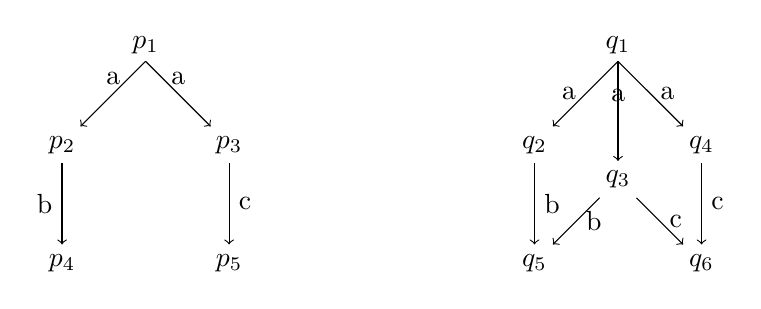
\begin{tikzpicture}[auto,node distance=1.5cm]
  \coordinate (p1) at (-3,0);
  \node at (-3, 0.2) {$p_1$}; 
  \node[below left of=p1] (p2) {$p_2$};
  \node[below right of=p1] (p3) {$p_3$};
  \node[below of=p2] (p4) {$p_4$};
  \node[below of=p3] (p5) {$p_5$};
  
  \draw[->] (p1) -- node[above] {a} (p2);
  \draw[->] (p1) -- node[above] {a} (p3);
  \draw[->] (p2) -- node[left] {b} (p4);
  \draw[->] (p3) -- node[right] {c} (p5);

\coordinate (q1) at (3,0);
  \node at (3, 0.2) {$q_1$}; 
  \node[below left of=q1] (q2) {$q_2$};
  \node[below of=q1] (q3) {$q_3$};
  \node[below right of=q1] (q4) {$q_4$};
  \node[below of=q2] (q5) {$q_5$};
  \node[below of=q4] (q6) {$q_6$};
  
  \draw[->] (q1) -- node[left] {a} (q2);
  \draw[->] (q1) -- node[above] {a} (q3);
  \draw[->] (q1) -- node[right] {a} (q4);
  \draw[->] (q2) -- node[right] {b} (q5);
  \draw[->] (q3) -- node[right] {b} (q5);
  \draw[->] (q3) -- node[right] {c} (q6);
  \draw[->] (q4) -- node[right] {c} (q6);
\end{tikzpicture}
\caption{TEEEEEEEEEEEEEEEEEEST}
    \label{fig:your_label}
\end{figure}%
\end{isamarkuptext}\isamarkuptrue%
\isacommand{definition}\isamarkupfalse%
\ expr{\isacharunderscore}{\kern0pt}ready{\isacharunderscore}{\kern0pt}trace\isanewline
\ \ \isakeyword{where}\isanewline
{\isachardoublequoteopen}expr{\isacharunderscore}{\kern0pt}ready{\isacharunderscore}{\kern0pt}trace\ {\isacharequal}{\kern0pt}\ {\isacharbraceleft}{\kern0pt}{\isasymphi}{\isachardot}{\kern0pt}\ {\isacharparenleft}{\kern0pt}less{\isacharunderscore}{\kern0pt}eq{\isacharunderscore}{\kern0pt}t\ {\isacharparenleft}{\kern0pt}expr\ {\isasymphi}{\isacharparenright}{\kern0pt}\ {\isacharparenleft}{\kern0pt}{\isasyminfinity}{\isacharcomma}{\kern0pt}\ {\isasyminfinity}{\isacharcomma}{\kern0pt}\ {\isasyminfinity}{\isacharcomma}{\kern0pt}\ {\isadigit{1}}{\isacharcomma}{\kern0pt}\ {\isadigit{1}}{\isacharcomma}{\kern0pt}\ {\isadigit{1}}{\isacharparenright}{\kern0pt}{\isacharparenright}{\kern0pt}{\isacharbraceright}{\kern0pt}{\isachardoublequoteclose}\isanewline
\isanewline
\isacommand{context}\isamarkupfalse%
\ lts\isanewline
\isakeyword{begin}\isanewline
\isanewline
\isacommand{definition}\isamarkupfalse%
\ expr{\isacharunderscore}{\kern0pt}ready{\isacharunderscore}{\kern0pt}trace{\isacharunderscore}{\kern0pt}equivalent\ \isanewline
\ \ \isakeyword{where}\isanewline
{\isachardoublequoteopen}expr{\isacharunderscore}{\kern0pt}ready{\isacharunderscore}{\kern0pt}trace{\isacharunderscore}{\kern0pt}equivalent\ p\ q\ {\isasymequiv}\ {\isacharparenleft}{\kern0pt}{\isasymforall}\ {\isasymphi}{\isachardot}{\kern0pt}\ {\isasymphi}\ {\isasymin}\ expr{\isacharunderscore}{\kern0pt}ready{\isacharunderscore}{\kern0pt}trace\ {\isasymlongrightarrow}\ {\isacharparenleft}{\kern0pt}p\ {\isasymTurnstile}\ {\isasymphi}{\isacharparenright}{\kern0pt}\ {\isasymlongleftrightarrow}\ {\isacharparenleft}{\kern0pt}q\ {\isasymTurnstile}\ {\isasymphi}{\isacharparenright}{\kern0pt}{\isacharparenright}{\kern0pt}{\isachardoublequoteclose}%
\begin{isamarkuptext}%
Proposition%
\end{isamarkuptext}\isamarkuptrue%
\isacommand{inductive}\isamarkupfalse%
\ HML{\isacharunderscore}{\kern0pt}revivals\ {\isacharcolon}{\kern0pt}{\isacharcolon}{\kern0pt}\ {\isachardoublequoteopen}{\isacharparenleft}{\kern0pt}{\isacharprime}{\kern0pt}a{\isacharcomma}{\kern0pt}\ {\isacharprime}{\kern0pt}s{\isacharparenright}{\kern0pt}\ hml\ {\isasymRightarrow}\ bool{\isachardoublequoteclose}\ \isanewline
\ \ \isakeyword{where}\isanewline
revivals{\isacharunderscore}{\kern0pt}tt{\isacharcolon}{\kern0pt}\ {\isachardoublequoteopen}HML{\isacharunderscore}{\kern0pt}revivals\ TT{\isachardoublequoteclose}\ {\isacharbar}{\kern0pt}\isanewline
revivals{\isacharunderscore}{\kern0pt}pos{\isacharcolon}{\kern0pt}\ {\isachardoublequoteopen}HML{\isacharunderscore}{\kern0pt}revivals\ {\isacharparenleft}{\kern0pt}hml{\isacharunderscore}{\kern0pt}pos\ {\isasymalpha}\ {\isasymphi}{\isacharparenright}{\kern0pt}{\isachardoublequoteclose}\ \isakeyword{if}\ {\isachardoublequoteopen}HML{\isacharunderscore}{\kern0pt}revivals\ {\isasymphi}{\isachardoublequoteclose}\ {\isacharbar}{\kern0pt}\isanewline
revivals{\isacharunderscore}{\kern0pt}conj{\isacharcolon}{\kern0pt}\ {\isachardoublequoteopen}HML{\isacharunderscore}{\kern0pt}revivals\ {\isacharparenleft}{\kern0pt}hml{\isacharunderscore}{\kern0pt}conj\ I\ J\ {\isasymPhi}{\isacharparenright}{\kern0pt}{\isachardoublequoteclose}\ \isakeyword{if}\ {\isachardoublequoteopen}{\isacharparenleft}{\kern0pt}{\isasymexists}x\ {\isasymin}\ {\isacharparenleft}{\kern0pt}{\isasymPhi}\ {\isacharbackquote}{\kern0pt}\ I{\isacharparenright}{\kern0pt}{\isachardot}{\kern0pt}\ {\isacharparenleft}{\kern0pt}{\isasymexists}{\isasymalpha}\ {\isasymchi}{\isachardot}{\kern0pt}\ {\isacharparenleft}{\kern0pt}x\ {\isacharequal}{\kern0pt}\ hml{\isacharunderscore}{\kern0pt}pos\ {\isasymalpha}\ {\isasymchi}{\isacharparenright}{\kern0pt}\ {\isasymand}\ TT{\isacharunderscore}{\kern0pt}like\ {\isasymchi}{\isacharparenright}{\kern0pt}\ {\isasymand}\ {\isacharparenleft}{\kern0pt}{\isasymforall}y\ {\isasymin}\ {\isacharparenleft}{\kern0pt}{\isasymPhi}\ {\isacharbackquote}{\kern0pt}\ I{\isacharparenright}{\kern0pt}{\isachardot}{\kern0pt}\ x\ {\isasymnoteq}\ y\ {\isasymlongrightarrow}\ TT{\isacharunderscore}{\kern0pt}like\ y{\isacharparenright}{\kern0pt}{\isacharparenright}{\kern0pt}\isanewline
{\isasymor}\ {\isacharparenleft}{\kern0pt}{\isasymforall}y\ {\isasymin}\ {\isacharparenleft}{\kern0pt}{\isasymPhi}\ {\isacharbackquote}{\kern0pt}\ I{\isacharparenright}{\kern0pt}{\isachardot}{\kern0pt}TT{\isacharunderscore}{\kern0pt}like\ y{\isacharparenright}{\kern0pt}{\isachardoublequoteclose}\isanewline
{\isachardoublequoteopen}{\isacharparenleft}{\kern0pt}{\isasymforall}x\ {\isasymin}\ {\isacharparenleft}{\kern0pt}{\isasymPhi}\ {\isacharbackquote}{\kern0pt}\ J{\isacharparenright}{\kern0pt}{\isachardot}{\kern0pt}\ TT{\isacharunderscore}{\kern0pt}like\ x\ {\isasymor}\ {\isacharparenleft}{\kern0pt}{\isasymexists}{\isasymalpha}\ {\isasymchi}{\isachardot}{\kern0pt}\ {\isacharparenleft}{\kern0pt}x\ {\isacharequal}{\kern0pt}\ hml{\isacharunderscore}{\kern0pt}pos\ {\isasymalpha}\ {\isasymchi}{\isacharparenright}{\kern0pt}\ {\isasymand}\ TT{\isacharunderscore}{\kern0pt}like\ {\isasymchi}{\isacharparenright}{\kern0pt}{\isacharparenright}{\kern0pt}{\isachardoublequoteclose}\isanewline
\isacommand{lemma}\isamarkupfalse%
\ revivals{\isacharunderscore}{\kern0pt}right{\isacharcolon}{\kern0pt}\isanewline
\ \ \isakeyword{assumes}\ {\isachardoublequoteopen}HML{\isacharunderscore}{\kern0pt}revivals\ {\isasymphi}{\isachardoublequoteclose}\isanewline
\ \ \isakeyword{shows}\ {\isachardoublequoteopen}less{\isacharunderscore}{\kern0pt}eq{\isacharunderscore}{\kern0pt}t\ {\isacharparenleft}{\kern0pt}expr\ {\isasymphi}{\isacharparenright}{\kern0pt}\ {\isacharparenleft}{\kern0pt}{\isasyminfinity}{\isacharcomma}{\kern0pt}\ {\isadigit{2}}{\isacharcomma}{\kern0pt}\ {\isadigit{1}}{\isacharcomma}{\kern0pt}\ {\isadigit{0}}{\isacharcomma}{\kern0pt}\ {\isadigit{1}}{\isacharcomma}{\kern0pt}\ {\isadigit{1}}{\isacharparenright}{\kern0pt}{\isachardoublequoteclose}\isanewline
%
\isadelimproof
\ \ %
\endisadelimproof
%
\isatagproof
\isacommand{using}\isamarkupfalse%
\ assms\isanewline
\isacommand{proof}\isamarkupfalse%
{\isacharparenleft}{\kern0pt}induction\ {\isasymphi}\ rule{\isacharcolon}{\kern0pt}\ HML{\isacharunderscore}{\kern0pt}revivals{\isachardot}{\kern0pt}induct{\isacharparenright}{\kern0pt}\isanewline
\ \ \isacommand{case}\isamarkupfalse%
\ revivals{\isacharunderscore}{\kern0pt}tt\isanewline
\ \ \isacommand{then}\isamarkupfalse%
\ \isacommand{show}\isamarkupfalse%
\ {\isacharquery}{\kern0pt}case\ \isacommand{by}\isamarkupfalse%
\ simp\isanewline
\isacommand{next}\isamarkupfalse%
\isanewline
\ \ \isacommand{case}\isamarkupfalse%
\ {\isacharparenleft}{\kern0pt}revivals{\isacharunderscore}{\kern0pt}pos\ {\isasymphi}\ {\isasymalpha}{\isacharparenright}{\kern0pt}\isanewline
\ \ \isacommand{then}\isamarkupfalse%
\ \isacommand{show}\isamarkupfalse%
\ {\isacharquery}{\kern0pt}case\ \isacommand{by}\isamarkupfalse%
\ simp\isanewline
\isacommand{next}\isamarkupfalse%
\isanewline
\ \ \isacommand{case}\isamarkupfalse%
\ {\isacharparenleft}{\kern0pt}revivals{\isacharunderscore}{\kern0pt}conj\ {\isasymPhi}\ I\ J{\isacharparenright}{\kern0pt}\isanewline
\ \ \isacommand{hence}\isamarkupfalse%
\ neg{\isacharcolon}{\kern0pt}\ {\isachardoublequoteopen}{\isasymforall}x{\isasymin}{\isasymPhi}\ {\isacharbackquote}{\kern0pt}\ J{\isachardot}{\kern0pt}\ less{\isacharunderscore}{\kern0pt}eq{\isacharunderscore}{\kern0pt}t\ {\isacharparenleft}{\kern0pt}expr\ x{\isacharparenright}{\kern0pt}\ {\isacharparenleft}{\kern0pt}{\isadigit{1}}{\isacharcomma}{\kern0pt}\ {\isadigit{1}}{\isacharcomma}{\kern0pt}\ {\isadigit{0}}{\isacharcomma}{\kern0pt}\ {\isadigit{0}}{\isacharcomma}{\kern0pt}\ {\isadigit{0}}{\isacharcomma}{\kern0pt}\ {\isadigit{0}}{\isacharparenright}{\kern0pt}{\isachardoublequoteclose}\isanewline
\ \ \ \ \isacommand{using}\isamarkupfalse%
\ e{\isadigit{1}}{\isacharunderscore}{\kern0pt}tt\ e{\isadigit{2}}{\isacharunderscore}{\kern0pt}tt\ e{\isadigit{3}}{\isacharunderscore}{\kern0pt}tt\ e{\isadigit{4}}{\isacharunderscore}{\kern0pt}tt\ e{\isadigit{5}}{\isacharunderscore}{\kern0pt}tt\ e{\isadigit{6}}{\isacharunderscore}{\kern0pt}tt\ expr{\isachardot}{\kern0pt}simps\ expr{\isacharunderscore}{\kern0pt}TT\ \isanewline
\ \ \ \ \isacommand{by}\isamarkupfalse%
\ {\isacharparenleft}{\kern0pt}metis\ le{\isacharunderscore}{\kern0pt}numeral{\isacharunderscore}{\kern0pt}extra{\isacharparenleft}{\kern0pt}{\isadigit{3}}{\isacharparenright}{\kern0pt}\ le{\isacharunderscore}{\kern0pt}numeral{\isacharunderscore}{\kern0pt}extra{\isacharparenleft}{\kern0pt}{\isadigit{4}}{\isacharparenright}{\kern0pt}\ less{\isacharunderscore}{\kern0pt}eq{\isacharunderscore}{\kern0pt}t{\isachardot}{\kern0pt}simps\ linordered{\isacharunderscore}{\kern0pt}nonzero{\isacharunderscore}{\kern0pt}semiring{\isacharunderscore}{\kern0pt}class{\isachardot}{\kern0pt}zero{\isacharunderscore}{\kern0pt}le{\isacharunderscore}{\kern0pt}one{\isacharparenright}{\kern0pt}\isanewline
\ \ \isacommand{hence}\isamarkupfalse%
\ f{\isadigit{2}}{\isacharcolon}{\kern0pt}\ {\isachardoublequoteopen}{\isasymforall}x\ {\isasymin}\ {\isacharparenleft}{\kern0pt}{\isacharparenleft}{\kern0pt}expr{\isacharunderscore}{\kern0pt}{\isadigit{1}}\ {\isasymcirc}\ {\isasymPhi}{\isacharparenright}{\kern0pt}\ {\isacharbackquote}{\kern0pt}\ J{\isacharparenright}{\kern0pt}{\isachardot}{\kern0pt}\ x\ {\isasymle}\ {\isadigit{1}}{\isachardoublequoteclose}\isanewline
\ \ \ {\isachardoublequoteopen}{\isasymforall}x\ {\isasymin}\ {\isacharparenleft}{\kern0pt}{\isacharparenleft}{\kern0pt}expr{\isacharunderscore}{\kern0pt}{\isadigit{2}}\ {\isasymcirc}\ {\isasymPhi}{\isacharparenright}{\kern0pt}\ {\isacharbackquote}{\kern0pt}\ J{\isacharparenright}{\kern0pt}{\isachardot}{\kern0pt}\ x\ {\isasymle}\ {\isadigit{1}}{\isachardoublequoteclose}\isanewline
\ \ \ {\isachardoublequoteopen}{\isasymforall}x\ {\isasymin}\ {\isacharparenleft}{\kern0pt}{\isacharparenleft}{\kern0pt}expr{\isacharunderscore}{\kern0pt}{\isadigit{3}}\ {\isasymcirc}\ {\isasymPhi}{\isacharparenright}{\kern0pt}\ {\isacharbackquote}{\kern0pt}\ J{\isacharparenright}{\kern0pt}{\isachardot}{\kern0pt}\ x\ {\isasymle}\ {\isadigit{0}}{\isachardoublequoteclose}\isanewline
\ \ \ {\isachardoublequoteopen}{\isasymforall}x\ {\isasymin}\ {\isacharparenleft}{\kern0pt}{\isacharparenleft}{\kern0pt}expr{\isacharunderscore}{\kern0pt}{\isadigit{4}}\ {\isasymcirc}\ {\isasymPhi}{\isacharparenright}{\kern0pt}\ {\isacharbackquote}{\kern0pt}\ J{\isacharparenright}{\kern0pt}{\isachardot}{\kern0pt}\ x\ {\isasymle}\ {\isadigit{0}}{\isachardoublequoteclose}\isanewline
\ \ \ {\isachardoublequoteopen}{\isasymforall}x\ {\isasymin}\ {\isacharparenleft}{\kern0pt}{\isacharparenleft}{\kern0pt}expr{\isacharunderscore}{\kern0pt}{\isadigit{5}}\ {\isasymcirc}\ {\isasymPhi}{\isacharparenright}{\kern0pt}\ {\isacharbackquote}{\kern0pt}\ J{\isacharparenright}{\kern0pt}{\isachardot}{\kern0pt}\ x\ {\isasymle}\ {\isadigit{0}}{\isachardoublequoteclose}\isanewline
\ \ \ {\isachardoublequoteopen}{\isasymforall}x\ {\isasymin}\ {\isacharparenleft}{\kern0pt}{\isacharparenleft}{\kern0pt}expr{\isacharunderscore}{\kern0pt}{\isadigit{6}}\ {\isasymcirc}\ {\isasymPhi}{\isacharparenright}{\kern0pt}\ {\isacharbackquote}{\kern0pt}\ J{\isacharparenright}{\kern0pt}{\isachardot}{\kern0pt}\ x\ {\isasymle}\ \ {\isadigit{0}}{\isachardoublequoteclose}\isanewline
\ \ \ \ \isacommand{using}\isamarkupfalse%
\ expr{\isachardot}{\kern0pt}simps\ \isacommand{by}\isamarkupfalse%
\ simp{\isacharplus}{\kern0pt}\isanewline
\isanewline
\isanewline
\ \ \isacommand{have}\isamarkupfalse%
\ {\isachardoublequoteopen}Sup\ {\isacharparenleft}{\kern0pt}{\isacharparenleft}{\kern0pt}expr{\isacharunderscore}{\kern0pt}{\isadigit{1}}\ {\isasymcirc}\ {\isasymPhi}{\isacharparenright}{\kern0pt}\ {\isacharbackquote}{\kern0pt}\ J{\isacharparenright}{\kern0pt}\ {\isasymle}\ {\isadigit{1}}{\isachardoublequoteclose}\isanewline
\isakeyword{and}\ {\isachardoublequoteopen}Sup\ {\isacharparenleft}{\kern0pt}{\isacharparenleft}{\kern0pt}expr{\isacharunderscore}{\kern0pt}{\isadigit{2}}\ {\isasymcirc}\ {\isasymPhi}{\isacharparenright}{\kern0pt}\ {\isacharbackquote}{\kern0pt}\ J{\isacharparenright}{\kern0pt}\ {\isasymle}\ {\isadigit{1}}{\isachardoublequoteclose}\isanewline
\isakeyword{and}\ {\isachardoublequoteopen}Sup\ {\isacharparenleft}{\kern0pt}{\isacharparenleft}{\kern0pt}expr{\isacharunderscore}{\kern0pt}{\isadigit{5}}\ {\isasymcirc}\ {\isasymPhi}{\isacharparenright}{\kern0pt}\ {\isacharbackquote}{\kern0pt}\ J{\isacharparenright}{\kern0pt}\ {\isasymle}\ {\isadigit{0}}{\isachardoublequoteclose}\isanewline
\isakeyword{and}\ {\isachardoublequoteopen}Sup\ {\isacharparenleft}{\kern0pt}{\isacharparenleft}{\kern0pt}expr{\isacharunderscore}{\kern0pt}{\isadigit{6}}\ {\isasymcirc}\ {\isasymPhi}{\isacharparenright}{\kern0pt}\ {\isacharbackquote}{\kern0pt}\ J{\isacharparenright}{\kern0pt}\ {\isasymle}\ {\isadigit{0}}{\isachardoublequoteclose}\isanewline
\isakeyword{and}\ {\isachardoublequoteopen}Sup\ {\isacharparenleft}{\kern0pt}{\isacharparenleft}{\kern0pt}expr{\isacharunderscore}{\kern0pt}{\isadigit{4}}\ {\isasymcirc}\ {\isasymPhi}{\isacharparenright}{\kern0pt}\ {\isacharbackquote}{\kern0pt}\ J{\isacharparenright}{\kern0pt}\ {\isasymle}\ {\isadigit{0}}{\isachardoublequoteclose}\isanewline
\isakeyword{and}\ {\isachardoublequoteopen}Sup\ {\isacharparenleft}{\kern0pt}{\isacharparenleft}{\kern0pt}expr{\isacharunderscore}{\kern0pt}{\isadigit{3}}\ {\isasymcirc}\ {\isasymPhi}{\isacharparenright}{\kern0pt}\ {\isacharbackquote}{\kern0pt}\ J{\isacharparenright}{\kern0pt}\ {\isasymle}\ {\isadigit{0}}{\isachardoublequoteclose}\ \isanewline
\isacommand{using}\isamarkupfalse%
\ Sup{\isacharunderscore}{\kern0pt}le{\isacharunderscore}{\kern0pt}iff\ f{\isadigit{2}}\isanewline
\ \ \ \ \ \ \ \ \ \isacommand{apply}\isamarkupfalse%
\ {\isacharparenleft}{\kern0pt}simp\ add{\isacharcolon}{\kern0pt}\ SUP{\isacharunderscore}{\kern0pt}least{\isacharparenright}{\kern0pt}\isanewline
\ \ \ \ \isacommand{using}\isamarkupfalse%
\ Sup{\isacharunderscore}{\kern0pt}le{\isacharunderscore}{\kern0pt}iff\ f{\isadigit{2}}\isanewline
\ \ \ \ \ \ \ \ \ \isacommand{apply}\isamarkupfalse%
\ {\isacharparenleft}{\kern0pt}simp\ add{\isacharcolon}{\kern0pt}\ SUP{\isacharunderscore}{\kern0pt}least{\isacharparenright}{\kern0pt}\isanewline
\ \ \ \ \isacommand{using}\isamarkupfalse%
\ Sup{\isacharunderscore}{\kern0pt}le{\isacharunderscore}{\kern0pt}iff\ f{\isadigit{2}}\isanewline
\ \ \ \ \isacommand{by}\isamarkupfalse%
\ {\isacharparenleft}{\kern0pt}metis{\isacharparenright}{\kern0pt}{\isacharplus}{\kern0pt}\isanewline
\ \ \isacommand{from}\isamarkupfalse%
\ revivals{\isacharunderscore}{\kern0pt}conj{\isacharparenleft}{\kern0pt}{\isadigit{1}}{\isacharparenright}{\kern0pt}\ \isacommand{show}\isamarkupfalse%
\ {\isacharquery}{\kern0pt}case\ \isacommand{proof}\isamarkupfalse%
\isanewline
\ \ \ \ \isacommand{assume}\isamarkupfalse%
\ {\isachardoublequoteopen}{\isasymforall}y{\isasymin}{\isasymPhi}\ {\isacharbackquote}{\kern0pt}\ I{\isachardot}{\kern0pt}\ TT{\isacharunderscore}{\kern0pt}like\ y{\isachardoublequoteclose}\isanewline
\ \ \ \ \isacommand{hence}\isamarkupfalse%
\ {\isachardoublequoteopen}{\isasymforall}y{\isasymin}{\isasymPhi}\ {\isacharbackquote}{\kern0pt}\ I{\isachardot}{\kern0pt}\ less{\isacharunderscore}{\kern0pt}eq{\isacharunderscore}{\kern0pt}t\ {\isacharparenleft}{\kern0pt}expr\ y{\isacharparenright}{\kern0pt}\ {\isacharparenleft}{\kern0pt}{\isadigit{0}}{\isacharcomma}{\kern0pt}\ {\isadigit{1}}{\isacharcomma}{\kern0pt}\ {\isadigit{0}}{\isacharcomma}{\kern0pt}\ {\isadigit{0}}{\isacharcomma}{\kern0pt}\ {\isadigit{0}}{\isacharcomma}{\kern0pt}\ {\isadigit{0}}{\isacharparenright}{\kern0pt}{\isachardoublequoteclose}\isanewline
\ \ \ \ \ \ \isacommand{using}\isamarkupfalse%
\ expr{\isacharunderscore}{\kern0pt}TT\ \isacommand{by}\isamarkupfalse%
\ auto\isanewline
\ \ \isacommand{hence}\isamarkupfalse%
\ f{\isadigit{1}}{\isacharcolon}{\kern0pt}\ {\isachardoublequoteopen}{\isasymforall}x\ {\isasymin}\ {\isacharparenleft}{\kern0pt}{\isacharparenleft}{\kern0pt}expr{\isacharunderscore}{\kern0pt}{\isadigit{1}}\ {\isasymcirc}\ {\isasymPhi}{\isacharparenright}{\kern0pt}\ {\isacharbackquote}{\kern0pt}\ I{\isacharparenright}{\kern0pt}{\isachardot}{\kern0pt}\ x\ {\isasymle}\ {\isadigit{0}}{\isachardoublequoteclose}\isanewline
\ \ \ {\isachardoublequoteopen}{\isasymforall}x\ {\isasymin}\ {\isacharparenleft}{\kern0pt}{\isacharparenleft}{\kern0pt}expr{\isacharunderscore}{\kern0pt}{\isadigit{2}}\ {\isasymcirc}\ {\isasymPhi}{\isacharparenright}{\kern0pt}\ {\isacharbackquote}{\kern0pt}\ I{\isacharparenright}{\kern0pt}{\isachardot}{\kern0pt}\ x\ {\isasymle}\ {\isadigit{1}}{\isachardoublequoteclose}\isanewline
\ \ \ {\isachardoublequoteopen}{\isasymforall}x\ {\isasymin}\ {\isacharparenleft}{\kern0pt}{\isacharparenleft}{\kern0pt}expr{\isacharunderscore}{\kern0pt}{\isadigit{3}}\ {\isasymcirc}\ {\isasymPhi}{\isacharparenright}{\kern0pt}\ {\isacharbackquote}{\kern0pt}\ I{\isacharparenright}{\kern0pt}{\isachardot}{\kern0pt}\ x\ {\isasymle}\ {\isadigit{0}}{\isachardoublequoteclose}\isanewline
\ \ \ {\isachardoublequoteopen}{\isasymforall}x\ {\isasymin}\ {\isacharparenleft}{\kern0pt}{\isacharparenleft}{\kern0pt}expr{\isacharunderscore}{\kern0pt}{\isadigit{4}}\ {\isasymcirc}\ {\isasymPhi}{\isacharparenright}{\kern0pt}\ {\isacharbackquote}{\kern0pt}\ I{\isacharparenright}{\kern0pt}{\isachardot}{\kern0pt}\ x\ {\isasymle}\ {\isadigit{0}}{\isachardoublequoteclose}\isanewline
\ \ \ {\isachardoublequoteopen}{\isasymforall}x\ {\isasymin}\ {\isacharparenleft}{\kern0pt}{\isacharparenleft}{\kern0pt}expr{\isacharunderscore}{\kern0pt}{\isadigit{5}}\ {\isasymcirc}\ {\isasymPhi}{\isacharparenright}{\kern0pt}\ {\isacharbackquote}{\kern0pt}\ I{\isacharparenright}{\kern0pt}{\isachardot}{\kern0pt}\ x\ {\isasymle}\ {\isadigit{0}}{\isachardoublequoteclose}\isanewline
\ \ \ {\isachardoublequoteopen}{\isasymforall}x\ {\isasymin}\ {\isacharparenleft}{\kern0pt}{\isacharparenleft}{\kern0pt}expr{\isacharunderscore}{\kern0pt}{\isadigit{6}}\ {\isasymcirc}\ {\isasymPhi}{\isacharparenright}{\kern0pt}\ {\isacharbackquote}{\kern0pt}\ I{\isacharparenright}{\kern0pt}{\isachardot}{\kern0pt}\ x\ {\isasymle}\ \ {\isadigit{0}}{\isachardoublequoteclose}\isanewline
\ \ \ \ \isacommand{using}\isamarkupfalse%
\ expr{\isachardot}{\kern0pt}simps\ \isacommand{by}\isamarkupfalse%
\ simp{\isacharplus}{\kern0pt}\isanewline
\isacommand{have}\isamarkupfalse%
\ {\isachardoublequoteopen}Sup\ {\isacharparenleft}{\kern0pt}{\isacharparenleft}{\kern0pt}expr{\isacharunderscore}{\kern0pt}{\isadigit{1}}\ {\isasymcirc}\ {\isasymPhi}{\isacharparenright}{\kern0pt}\ {\isacharbackquote}{\kern0pt}\ I{\isacharparenright}{\kern0pt}\ {\isasymle}\ {\isadigit{0}}{\isachardoublequoteclose}\isanewline
\isakeyword{and}\ {\isachardoublequoteopen}Sup\ {\isacharparenleft}{\kern0pt}{\isacharparenleft}{\kern0pt}expr{\isacharunderscore}{\kern0pt}{\isadigit{2}}\ {\isasymcirc}\ {\isasymPhi}{\isacharparenright}{\kern0pt}\ {\isacharbackquote}{\kern0pt}\ I{\isacharparenright}{\kern0pt}\ {\isasymle}\ {\isadigit{1}}{\isachardoublequoteclose}\isanewline
\isakeyword{and}\ {\isachardoublequoteopen}Sup\ {\isacharparenleft}{\kern0pt}{\isacharparenleft}{\kern0pt}expr{\isacharunderscore}{\kern0pt}{\isadigit{5}}\ {\isasymcirc}\ {\isasymPhi}{\isacharparenright}{\kern0pt}\ {\isacharbackquote}{\kern0pt}\ I{\isacharparenright}{\kern0pt}\ {\isasymle}\ {\isadigit{0}}{\isachardoublequoteclose}\isanewline
\isakeyword{and}\ {\isachardoublequoteopen}Sup\ {\isacharparenleft}{\kern0pt}{\isacharparenleft}{\kern0pt}expr{\isacharunderscore}{\kern0pt}{\isadigit{6}}\ {\isasymcirc}\ {\isasymPhi}{\isacharparenright}{\kern0pt}\ {\isacharbackquote}{\kern0pt}\ I{\isacharparenright}{\kern0pt}\ {\isasymle}\ {\isadigit{0}}{\isachardoublequoteclose}\isanewline
\isakeyword{and}\ {\isachardoublequoteopen}Sup\ {\isacharparenleft}{\kern0pt}{\isacharparenleft}{\kern0pt}expr{\isacharunderscore}{\kern0pt}{\isadigit{4}}\ {\isasymcirc}\ {\isasymPhi}{\isacharparenright}{\kern0pt}\ {\isacharbackquote}{\kern0pt}\ I{\isacharparenright}{\kern0pt}\ {\isasymle}\ {\isadigit{0}}{\isachardoublequoteclose}\isanewline
\isakeyword{and}\ {\isachardoublequoteopen}Sup\ {\isacharparenleft}{\kern0pt}{\isacharparenleft}{\kern0pt}expr{\isacharunderscore}{\kern0pt}{\isadigit{3}}\ {\isasymcirc}\ {\isasymPhi}{\isacharparenright}{\kern0pt}\ {\isacharbackquote}{\kern0pt}\ I{\isacharparenright}{\kern0pt}\ {\isasymle}\ {\isadigit{0}}{\isachardoublequoteclose}\isanewline
\ \ \ \ \isacommand{using}\isamarkupfalse%
\ Sup{\isacharunderscore}{\kern0pt}le{\isacharunderscore}{\kern0pt}iff\ f{\isadigit{1}}\isanewline
\ \ \ \ \ \ \ \ \ \isacommand{apply}\isamarkupfalse%
\ {\isacharparenleft}{\kern0pt}simp\ add{\isacharcolon}{\kern0pt}\ SUP{\isacharunderscore}{\kern0pt}least{\isacharparenright}{\kern0pt}\isanewline
\ \ \ \ \isacommand{using}\isamarkupfalse%
\ Sup{\isacharunderscore}{\kern0pt}le{\isacharunderscore}{\kern0pt}iff\ f{\isadigit{1}}\isanewline
\ \ \ \ \ \ \ \ \ \isacommand{apply}\isamarkupfalse%
\ {\isacharparenleft}{\kern0pt}simp\ add{\isacharcolon}{\kern0pt}\ SUP{\isacharunderscore}{\kern0pt}least{\isacharparenright}{\kern0pt}\isanewline
\ \ \ \ \isacommand{using}\isamarkupfalse%
\ Sup{\isacharunderscore}{\kern0pt}le{\isacharunderscore}{\kern0pt}iff\ f{\isadigit{1}}\ SUP{\isacharunderscore}{\kern0pt}bot{\isacharunderscore}{\kern0pt}conv{\isacharparenleft}{\kern0pt}{\isadigit{2}}{\isacharparenright}{\kern0pt}\ bot{\isacharunderscore}{\kern0pt}enat{\isacharunderscore}{\kern0pt}def\isanewline
\ \ \ \ \isacommand{by}\isamarkupfalse%
\ {\isacharparenleft}{\kern0pt}metis\ {\isacharparenright}{\kern0pt}{\isacharplus}{\kern0pt}\isanewline
\ \ \isacommand{have}\isamarkupfalse%
\ e{\isadigit{2}}{\isacharcolon}{\kern0pt}\ {\isachardoublequoteopen}expr{\isacharunderscore}{\kern0pt}{\isadigit{2}}\ {\isacharparenleft}{\kern0pt}hml{\isacharunderscore}{\kern0pt}conj\ I\ J\ {\isasymPhi}{\isacharparenright}{\kern0pt}\ {\isasymle}\ {\isadigit{2}}{\isachardoublequoteclose}\isanewline
\ \ \ \ \isacommand{using}\isamarkupfalse%
\ {\isacartoucheopen}Sup\ {\isacharparenleft}{\kern0pt}{\isacharparenleft}{\kern0pt}expr{\isacharunderscore}{\kern0pt}{\isadigit{2}}\ {\isasymcirc}\ {\isasymPhi}{\isacharparenright}{\kern0pt}\ {\isacharbackquote}{\kern0pt}\ I{\isacharparenright}{\kern0pt}\ {\isasymle}\ {\isadigit{1}}{\isacartoucheclose}\ {\isacartoucheopen}Sup\ {\isacharparenleft}{\kern0pt}{\isacharparenleft}{\kern0pt}expr{\isacharunderscore}{\kern0pt}{\isadigit{2}}\ {\isasymcirc}\ {\isasymPhi}{\isacharparenright}{\kern0pt}\ {\isacharbackquote}{\kern0pt}\ J{\isacharparenright}{\kern0pt}\ {\isasymle}\ {\isadigit{1}}{\isacartoucheclose}\ expr{\isacharunderscore}{\kern0pt}{\isadigit{2}}{\isacharunderscore}{\kern0pt}conj\ one{\isacharunderscore}{\kern0pt}add{\isacharunderscore}{\kern0pt}one\isanewline
\ \ \ \ \isacommand{by}\isamarkupfalse%
\ {\isacharparenleft}{\kern0pt}metis\ Sup{\isacharunderscore}{\kern0pt}union{\isacharunderscore}{\kern0pt}distrib\ add{\isacharunderscore}{\kern0pt}left{\isacharunderscore}{\kern0pt}mono\ le{\isacharunderscore}{\kern0pt}sup{\isacharunderscore}{\kern0pt}iff{\isacharparenright}{\kern0pt}\isanewline
\ \ \isacommand{have}\isamarkupfalse%
\ e{\isadigit{3}}{\isacharcolon}{\kern0pt}\ {\isachardoublequoteopen}expr{\isacharunderscore}{\kern0pt}{\isadigit{3}}\ {\isacharparenleft}{\kern0pt}hml{\isacharunderscore}{\kern0pt}conj\ I\ J\ {\isasymPhi}{\isacharparenright}{\kern0pt}\ {\isasymle}\ {\isadigit{1}}{\isachardoublequoteclose}\isanewline
\ \ \ \ \isacommand{using}\isamarkupfalse%
\ {\isacartoucheopen}Sup\ {\isacharparenleft}{\kern0pt}{\isacharparenleft}{\kern0pt}expr{\isacharunderscore}{\kern0pt}{\isadigit{1}}\ {\isasymcirc}\ {\isasymPhi}{\isacharparenright}{\kern0pt}\ {\isacharbackquote}{\kern0pt}\ I{\isacharparenright}{\kern0pt}\ {\isasymle}\ {\isadigit{0}}{\isacartoucheclose}\ {\isacartoucheopen}Sup\ {\isacharparenleft}{\kern0pt}{\isacharparenleft}{\kern0pt}expr{\isacharunderscore}{\kern0pt}{\isadigit{3}}\ {\isasymcirc}\ {\isasymPhi}{\isacharparenright}{\kern0pt}\ {\isacharbackquote}{\kern0pt}\ J{\isacharparenright}{\kern0pt}\ {\isasymle}\ {\isadigit{0}}{\isacartoucheclose}\ {\isacartoucheopen}Sup\ {\isacharparenleft}{\kern0pt}{\isacharparenleft}{\kern0pt}expr{\isacharunderscore}{\kern0pt}{\isadigit{3}}\ {\isasymcirc}\ {\isasymPhi}{\isacharparenright}{\kern0pt}\ {\isacharbackquote}{\kern0pt}\ I{\isacharparenright}{\kern0pt}\ {\isasymle}\ {\isadigit{0}}{\isacartoucheclose}\ \isanewline
\ \ \ \ \ \ one{\isacharunderscore}{\kern0pt}add{\isacharunderscore}{\kern0pt}one\ expr{\isacharunderscore}{\kern0pt}{\isadigit{3}}{\isacharunderscore}{\kern0pt}conj\ Sup{\isacharunderscore}{\kern0pt}union{\isacharunderscore}{\kern0pt}distrib\ add{\isacharunderscore}{\kern0pt}left{\isacharunderscore}{\kern0pt}mono\ le{\isacharunderscore}{\kern0pt}sup{\isacharunderscore}{\kern0pt}iff\isanewline
\ \ \ \ \isacommand{by}\isamarkupfalse%
\ {\isacharparenleft}{\kern0pt}smt\ {\isacharparenleft}{\kern0pt}verit{\isacharparenright}{\kern0pt}\ le{\isacharunderscore}{\kern0pt}zero{\isacharunderscore}{\kern0pt}eq\ max{\isacharunderscore}{\kern0pt}def\ sup{\isacharunderscore}{\kern0pt}enat{\isacharunderscore}{\kern0pt}def{\isacharparenright}{\kern0pt}\isanewline
\ \ \isacommand{from}\isamarkupfalse%
\ {\isacartoucheopen}Sup\ {\isacharparenleft}{\kern0pt}{\isacharparenleft}{\kern0pt}expr{\isacharunderscore}{\kern0pt}{\isadigit{1}}\ {\isasymcirc}\ {\isasymPhi}{\isacharparenright}{\kern0pt}\ {\isacharbackquote}{\kern0pt}\ I{\isacharparenright}{\kern0pt}\ {\isasymle}\ {\isadigit{0}}{\isacartoucheclose}\ \isacommand{have}\isamarkupfalse%
\ {\isachardoublequoteopen}Sup\ {\isacharparenleft}{\kern0pt}expr{\isacharunderscore}{\kern0pt}{\isadigit{1}}\ {\isacharbackquote}{\kern0pt}\ {\isacharparenleft}{\kern0pt}pos{\isacharunderscore}{\kern0pt}r\ {\isacharparenleft}{\kern0pt}{\isasymPhi}\ {\isacharbackquote}{\kern0pt}\ I{\isacharparenright}{\kern0pt}{\isacharparenright}{\kern0pt}{\isacharparenright}{\kern0pt}\ {\isacharless}{\kern0pt}{\isacharequal}{\kern0pt}\ {\isadigit{0}}{\isachardoublequoteclose}\ \isanewline
\ \ \ \ \isacommand{using}\isamarkupfalse%
\ SUP{\isacharunderscore}{\kern0pt}image\ dual{\isacharunderscore}{\kern0pt}order{\isachardot}{\kern0pt}trans\ mon{\isacharunderscore}{\kern0pt}expr{\isacharunderscore}{\kern0pt}{\isadigit{1}}{\isacharunderscore}{\kern0pt}pos{\isacharunderscore}{\kern0pt}r\ \isacommand{by}\isamarkupfalse%
\ metis\isanewline
\ \ \isacommand{hence}\isamarkupfalse%
\ e{\isadigit{4}}{\isacharcolon}{\kern0pt}\ {\isachardoublequoteopen}expr{\isacharunderscore}{\kern0pt}{\isadigit{4}}\ {\isacharparenleft}{\kern0pt}hml{\isacharunderscore}{\kern0pt}conj\ I\ J\ {\isasymPhi}{\isacharparenright}{\kern0pt}\ {\isasymle}\ {\isadigit{0}}{\isachardoublequoteclose}\ \isanewline
\ \ \ \ \isacommand{using}\isamarkupfalse%
\ {\isacartoucheopen}Sup\ {\isacharparenleft}{\kern0pt}{\isacharparenleft}{\kern0pt}expr{\isacharunderscore}{\kern0pt}{\isadigit{4}}\ {\isasymcirc}\ {\isasymPhi}{\isacharparenright}{\kern0pt}\ {\isacharbackquote}{\kern0pt}\ I{\isacharparenright}{\kern0pt}\ {\isasymle}\ {\isadigit{0}}{\isacartoucheclose}\ {\isacartoucheopen}Sup\ {\isacharparenleft}{\kern0pt}{\isacharparenleft}{\kern0pt}expr{\isacharunderscore}{\kern0pt}{\isadigit{4}}\ {\isasymcirc}\ {\isasymPhi}{\isacharparenright}{\kern0pt}\ {\isacharbackquote}{\kern0pt}\ J{\isacharparenright}{\kern0pt}\ {\isasymle}\ {\isadigit{0}}{\isacartoucheclose}\isanewline
\ \ \ \ \ \ expr{\isacharunderscore}{\kern0pt}{\isadigit{4}}{\isacharunderscore}{\kern0pt}conj\ Sup{\isacharunderscore}{\kern0pt}union{\isacharunderscore}{\kern0pt}distrib\ le{\isacharunderscore}{\kern0pt}sup{\isacharunderscore}{\kern0pt}iff\isanewline
\ \ \ \ \isacommand{by}\isamarkupfalse%
\ metis\isanewline
\ \ \isacommand{have}\isamarkupfalse%
\ e{\isadigit{5}}{\isacharcolon}{\kern0pt}\ {\isachardoublequoteopen}expr{\isacharunderscore}{\kern0pt}{\isadigit{5}}\ {\isacharparenleft}{\kern0pt}hml{\isacharunderscore}{\kern0pt}conj\ I\ J\ {\isasymPhi}{\isacharparenright}{\kern0pt}\ {\isasymle}\ {\isadigit{1}}{\isachardoublequoteclose}\ \isanewline
\ \ \ \ \isacommand{using}\isamarkupfalse%
\ {\isacartoucheopen}Sup\ {\isacharparenleft}{\kern0pt}{\isacharparenleft}{\kern0pt}expr{\isacharunderscore}{\kern0pt}{\isadigit{5}}\ {\isasymcirc}\ {\isasymPhi}{\isacharparenright}{\kern0pt}\ {\isacharbackquote}{\kern0pt}\ I{\isacharparenright}{\kern0pt}\ {\isasymle}\ {\isadigit{0}}{\isacartoucheclose}\ {\isacartoucheopen}Sup\ {\isacharparenleft}{\kern0pt}{\isacharparenleft}{\kern0pt}expr{\isacharunderscore}{\kern0pt}{\isadigit{5}}\ {\isasymcirc}\ {\isasymPhi}{\isacharparenright}{\kern0pt}\ {\isacharbackquote}{\kern0pt}\ J{\isacharparenright}{\kern0pt}\ {\isasymle}\ {\isadigit{0}}{\isacartoucheclose}\ {\isacartoucheopen}Sup\ {\isacharparenleft}{\kern0pt}{\isacharparenleft}{\kern0pt}expr{\isacharunderscore}{\kern0pt}{\isadigit{1}}\ {\isasymcirc}\ {\isasymPhi}{\isacharparenright}{\kern0pt}\ {\isacharbackquote}{\kern0pt}\ J{\isacharparenright}{\kern0pt}\ {\isasymle}\ {\isadigit{1}}{\isacartoucheclose}\ expr{\isacharunderscore}{\kern0pt}{\isadigit{5}}{\isacharunderscore}{\kern0pt}conj\ \isanewline
\ \ \ \ \isacommand{by}\isamarkupfalse%
\ {\isacharparenleft}{\kern0pt}simp\ add{\isacharcolon}{\kern0pt}\ Sup{\isacharunderscore}{\kern0pt}union{\isacharunderscore}{\kern0pt}distrib{\isacharparenright}{\kern0pt}\isanewline
\ \ \isacommand{from}\isamarkupfalse%
\ {\isacartoucheopen}Sup\ {\isacharparenleft}{\kern0pt}{\isacharparenleft}{\kern0pt}expr{\isacharunderscore}{\kern0pt}{\isadigit{6}}\ {\isasymcirc}\ {\isasymPhi}{\isacharparenright}{\kern0pt}\ {\isacharbackquote}{\kern0pt}\ J{\isacharparenright}{\kern0pt}\ {\isasymle}\ {\isadigit{0}}{\isacartoucheclose}\ \isacommand{have}\isamarkupfalse%
\ {\isachardoublequoteopen}Sup\ {\isacharparenleft}{\kern0pt}{\isacharparenleft}{\kern0pt}eSuc\ {\isasymcirc}\ expr{\isacharunderscore}{\kern0pt}{\isadigit{6}}\ {\isasymcirc}\ {\isasymPhi}{\isacharparenright}{\kern0pt}\ {\isacharbackquote}{\kern0pt}\ J{\isacharparenright}{\kern0pt}\ {\isasymle}\ {\isadigit{1}}{\isachardoublequoteclose}\isanewline
\ \ \ \ \isacommand{using}\isamarkupfalse%
\ eSuc{\isacharunderscore}{\kern0pt}def\ f{\isadigit{2}}{\isacharparenleft}{\kern0pt}{\isadigit{6}}{\isacharparenright}{\kern0pt}\isanewline
\ \ \ \ \isacommand{by}\isamarkupfalse%
\ {\isacharparenleft}{\kern0pt}metis\ eSuc{\isacharunderscore}{\kern0pt}Sup\ image{\isacharunderscore}{\kern0pt}comp\ image{\isacharunderscore}{\kern0pt}is{\isacharunderscore}{\kern0pt}empty\ nle{\isacharunderscore}{\kern0pt}le\ one{\isacharunderscore}{\kern0pt}eSuc\ zero{\isacharunderscore}{\kern0pt}le{\isacharparenright}{\kern0pt}\ \isanewline
\ \ \ \ \isacommand{hence}\isamarkupfalse%
\ e{\isadigit{6}}{\isacharcolon}{\kern0pt}\ {\isachardoublequoteopen}expr{\isacharunderscore}{\kern0pt}{\isadigit{6}}\ {\isacharparenleft}{\kern0pt}hml{\isacharunderscore}{\kern0pt}conj\ I\ J\ {\isasymPhi}{\isacharparenright}{\kern0pt}\ {\isasymle}\ {\isadigit{1}}{\isachardoublequoteclose}\isanewline
\ \ \ \ \isacommand{using}\isamarkupfalse%
\ {\isacartoucheopen}Sup\ {\isacharparenleft}{\kern0pt}{\isacharparenleft}{\kern0pt}expr{\isacharunderscore}{\kern0pt}{\isadigit{6}}\ {\isasymcirc}\ {\isasymPhi}{\isacharparenright}{\kern0pt}\ {\isacharbackquote}{\kern0pt}\ I{\isacharparenright}{\kern0pt}\ {\isasymle}\ {\isadigit{0}}{\isacartoucheclose}\ expr{\isacharunderscore}{\kern0pt}{\isadigit{6}}{\isacharunderscore}{\kern0pt}conj\ \isanewline
\ \ \ \ \isacommand{by}\isamarkupfalse%
\ {\isacharparenleft}{\kern0pt}simp\ add{\isacharcolon}{\kern0pt}\ Sup{\isacharunderscore}{\kern0pt}union{\isacharunderscore}{\kern0pt}distrib{\isacharparenright}{\kern0pt}\isanewline
\ \ \isacommand{then}\isamarkupfalse%
\ \isacommand{show}\isamarkupfalse%
\ {\isacharquery}{\kern0pt}thesis\ \isacommand{using}\isamarkupfalse%
\ e{\isadigit{2}}\ e{\isadigit{3}}\ e{\isadigit{4}}\ e{\isadigit{5}}\ e{\isadigit{6}}\ expr{\isachardot}{\kern0pt}simps\ less{\isacharunderscore}{\kern0pt}eq{\isacharunderscore}{\kern0pt}t{\isachardot}{\kern0pt}simps\ \isanewline
\ \ \ \ \isacommand{by}\isamarkupfalse%
\ {\isacharparenleft}{\kern0pt}metis\ enat{\isacharunderscore}{\kern0pt}ord{\isacharunderscore}{\kern0pt}code{\isacharparenleft}{\kern0pt}{\isadigit{3}}{\isacharparenright}{\kern0pt}{\isacharparenright}{\kern0pt}\isanewline
\isacommand{next}\isamarkupfalse%
\isanewline
\ \ \isacommand{assume}\isamarkupfalse%
\ {\isachardoublequoteopen}{\isasymexists}x{\isasymin}{\isasymPhi}\ {\isacharbackquote}{\kern0pt}\ I{\isachardot}{\kern0pt}\ {\isacharparenleft}{\kern0pt}{\isasymexists}{\isasymalpha}\ {\isasymchi}{\isachardot}{\kern0pt}\ x\ {\isacharequal}{\kern0pt}\ hml{\isacharunderscore}{\kern0pt}pos\ {\isasymalpha}\ {\isasymchi}\ {\isasymand}\ TT{\isacharunderscore}{\kern0pt}like\ {\isasymchi}{\isacharparenright}{\kern0pt}\ {\isasymand}\ {\isacharparenleft}{\kern0pt}{\isasymforall}y{\isasymin}{\isasymPhi}\ {\isacharbackquote}{\kern0pt}\ I{\isachardot}{\kern0pt}\ x\ {\isasymnoteq}\ y\ {\isasymlongrightarrow}\ TT{\isacharunderscore}{\kern0pt}like\ y{\isacharparenright}{\kern0pt}{\isachardoublequoteclose}\isanewline
\ \ \isacommand{then}\isamarkupfalse%
\ \isacommand{obtain}\isamarkupfalse%
\ {\isasymphi}\ \isakeyword{where}\ {\isachardoublequoteopen}{\isasymphi}\ {\isasymin}\ {\isasymPhi}\ {\isacharbackquote}{\kern0pt}\ I{\isachardoublequoteclose}\ {\isachardoublequoteopen}{\isacharparenleft}{\kern0pt}{\isasymexists}{\isasymalpha}\ {\isasymchi}{\isachardot}{\kern0pt}\ {\isasymphi}\ {\isacharequal}{\kern0pt}\ hml{\isacharunderscore}{\kern0pt}pos\ {\isasymalpha}\ {\isasymchi}\ {\isasymand}\ TT{\isacharunderscore}{\kern0pt}like\ {\isasymchi}{\isacharparenright}{\kern0pt}{\isachardoublequoteclose}\ {\isachardoublequoteopen}{\isacharparenleft}{\kern0pt}{\isasymforall}y{\isasymin}{\isasymPhi}\ {\isacharbackquote}{\kern0pt}\ I{\isachardot}{\kern0pt}\ {\isasymphi}\ {\isasymnoteq}\ y\ {\isasymlongrightarrow}\ TT{\isacharunderscore}{\kern0pt}like\ y{\isacharparenright}{\kern0pt}{\isachardoublequoteclose}\isanewline
\ \ \ \ \isacommand{by}\isamarkupfalse%
\ blast\isanewline
\ \ \isacommand{hence}\isamarkupfalse%
\ expr{\isacharunderscore}{\kern0pt}{\isasymphi}{\isacharcolon}{\kern0pt}\ {\isachardoublequoteopen}expr{\isacharunderscore}{\kern0pt}{\isadigit{1}}\ {\isasymphi}\ {\isacharequal}{\kern0pt}\ {\isadigit{1}}{\isachardoublequoteclose}\ {\isachardoublequoteopen}expr{\isacharunderscore}{\kern0pt}{\isadigit{2}}\ {\isasymphi}\ {\isacharequal}{\kern0pt}\ {\isadigit{1}}{\isachardoublequoteclose}\ {\isachardoublequoteopen}expr{\isacharunderscore}{\kern0pt}{\isadigit{3}}\ {\isasymphi}\ {\isacharequal}{\kern0pt}\ {\isadigit{0}}{\isachardoublequoteclose}\ {\isachardoublequoteopen}expr{\isacharunderscore}{\kern0pt}{\isadigit{4}}\ {\isasymphi}\ {\isacharequal}{\kern0pt}\ {\isadigit{0}}{\isachardoublequoteclose}\ {\isachardoublequoteopen}expr{\isacharunderscore}{\kern0pt}{\isadigit{5}}\ {\isasymphi}\ {\isacharequal}{\kern0pt}\ {\isadigit{0}}{\isachardoublequoteclose}\ {\isachardoublequoteopen}expr{\isacharunderscore}{\kern0pt}{\isadigit{6}}\ {\isasymphi}\ {\isacharequal}{\kern0pt}\ {\isadigit{0}}{\isachardoublequoteclose}\isanewline
\ \ \ \ \isacommand{using}\isamarkupfalse%
\ e{\isadigit{1}}{\isacharunderscore}{\kern0pt}tt\ e{\isadigit{2}}{\isacharunderscore}{\kern0pt}tt\ e{\isadigit{3}}{\isacharunderscore}{\kern0pt}tt\ e{\isadigit{4}}{\isacharunderscore}{\kern0pt}tt\ e{\isadigit{5}}{\isacharunderscore}{\kern0pt}tt\ e{\isadigit{6}}{\isacharunderscore}{\kern0pt}tt\ expr{\isachardot}{\kern0pt}simps\ expr{\isacharunderscore}{\kern0pt}TT\ \isanewline
\ \ \ \ \isacommand{by}\isamarkupfalse%
\ metis{\isacharplus}{\kern0pt}\isanewline
\ \ \isacommand{have}\isamarkupfalse%
\ {\isachardoublequoteopen}{\isacharparenleft}{\kern0pt}{\isasymforall}y{\isasymin}{\isasymPhi}\ {\isacharbackquote}{\kern0pt}\ I{\isachardot}{\kern0pt}\ {\isasymphi}\ {\isasymnoteq}\ y\ {\isasymlongrightarrow}\ expr{\isacharunderscore}{\kern0pt}{\isadigit{1}}\ y\ {\isacharequal}{\kern0pt}\ {\isadigit{0}}{\isacharparenright}{\kern0pt}{\isachardoublequoteclose}\isanewline
{\isachardoublequoteopen}{\isacharparenleft}{\kern0pt}{\isasymforall}y{\isasymin}{\isasymPhi}\ {\isacharbackquote}{\kern0pt}\ I{\isachardot}{\kern0pt}\ {\isasymphi}\ {\isasymnoteq}\ y\ {\isasymlongrightarrow}\ expr{\isacharunderscore}{\kern0pt}{\isadigit{2}}\ y\ {\isacharequal}{\kern0pt}\ {\isadigit{1}}{\isacharparenright}{\kern0pt}{\isachardoublequoteclose}\isanewline
{\isachardoublequoteopen}{\isacharparenleft}{\kern0pt}{\isasymforall}y{\isasymin}{\isasymPhi}\ {\isacharbackquote}{\kern0pt}\ I{\isachardot}{\kern0pt}\ {\isasymphi}\ {\isasymnoteq}\ y\ {\isasymlongrightarrow}\ expr{\isacharunderscore}{\kern0pt}{\isadigit{3}}\ y\ {\isacharequal}{\kern0pt}\ {\isadigit{0}}{\isacharparenright}{\kern0pt}{\isachardoublequoteclose}\isanewline
{\isachardoublequoteopen}{\isacharparenleft}{\kern0pt}{\isasymforall}y{\isasymin}{\isasymPhi}\ {\isacharbackquote}{\kern0pt}\ I{\isachardot}{\kern0pt}\ {\isasymphi}\ {\isasymnoteq}\ y\ {\isasymlongrightarrow}\ expr{\isacharunderscore}{\kern0pt}{\isadigit{4}}\ y\ {\isacharequal}{\kern0pt}\ {\isadigit{0}}{\isacharparenright}{\kern0pt}{\isachardoublequoteclose}\isanewline
{\isachardoublequoteopen}{\isacharparenleft}{\kern0pt}{\isasymforall}y{\isasymin}{\isasymPhi}\ {\isacharbackquote}{\kern0pt}\ I{\isachardot}{\kern0pt}\ {\isasymphi}\ {\isasymnoteq}\ y\ {\isasymlongrightarrow}\ expr{\isacharunderscore}{\kern0pt}{\isadigit{5}}\ y\ {\isacharequal}{\kern0pt}\ {\isadigit{0}}{\isacharparenright}{\kern0pt}{\isachardoublequoteclose}\isanewline
{\isachardoublequoteopen}{\isacharparenleft}{\kern0pt}{\isasymforall}y{\isasymin}{\isasymPhi}\ {\isacharbackquote}{\kern0pt}\ I{\isachardot}{\kern0pt}\ {\isasymphi}\ {\isasymnoteq}\ y\ {\isasymlongrightarrow}\ expr{\isacharunderscore}{\kern0pt}{\isadigit{6}}\ y\ {\isacharequal}{\kern0pt}\ {\isadigit{0}}{\isacharparenright}{\kern0pt}{\isachardoublequoteclose}\isanewline
\ \ \ \ \isacommand{using}\isamarkupfalse%
\ {\isacartoucheopen}{\isacharparenleft}{\kern0pt}{\isasymforall}y{\isasymin}{\isasymPhi}\ {\isacharbackquote}{\kern0pt}\ I{\isachardot}{\kern0pt}\ {\isasymphi}\ {\isasymnoteq}\ y\ {\isasymlongrightarrow}\ TT{\isacharunderscore}{\kern0pt}like\ y{\isacharparenright}{\kern0pt}{\isacartoucheclose}\ expr{\isacharunderscore}{\kern0pt}TT\ expr{\isachardot}{\kern0pt}simps\ \isanewline
\ \ \ \ \isacommand{by}\isamarkupfalse%
\ fastforce{\isacharplus}{\kern0pt}\isanewline
\ \ \isacommand{hence}\isamarkupfalse%
\ {\isachardoublequoteopen}Sup\ {\isacharparenleft}{\kern0pt}{\isacharparenleft}{\kern0pt}expr{\isacharunderscore}{\kern0pt}{\isadigit{1}}\ {\isasymcirc}\ {\isasymPhi}{\isacharparenright}{\kern0pt}\ {\isacharbackquote}{\kern0pt}\ I{\isacharparenright}{\kern0pt}\ {\isasymle}\ {\isadigit{1}}{\isachardoublequoteclose}\isanewline
{\isachardoublequoteopen}Sup\ {\isacharparenleft}{\kern0pt}{\isacharparenleft}{\kern0pt}expr{\isacharunderscore}{\kern0pt}{\isadigit{2}}\ {\isasymcirc}\ {\isasymPhi}{\isacharparenright}{\kern0pt}\ {\isacharbackquote}{\kern0pt}\ I{\isacharparenright}{\kern0pt}\ {\isasymle}\ {\isadigit{1}}{\isachardoublequoteclose}\isanewline
{\isachardoublequoteopen}Sup\ {\isacharparenleft}{\kern0pt}{\isacharparenleft}{\kern0pt}expr{\isacharunderscore}{\kern0pt}{\isadigit{3}}\ {\isasymcirc}\ {\isasymPhi}{\isacharparenright}{\kern0pt}\ {\isacharbackquote}{\kern0pt}\ I{\isacharparenright}{\kern0pt}\ {\isasymle}\ {\isadigit{0}}{\isachardoublequoteclose}\isanewline
{\isachardoublequoteopen}Sup\ {\isacharparenleft}{\kern0pt}{\isacharparenleft}{\kern0pt}expr{\isacharunderscore}{\kern0pt}{\isadigit{4}}\ {\isasymcirc}\ {\isasymPhi}{\isacharparenright}{\kern0pt}\ {\isacharbackquote}{\kern0pt}\ I{\isacharparenright}{\kern0pt}\ {\isasymle}\ {\isadigit{0}}{\isachardoublequoteclose}\isanewline
{\isachardoublequoteopen}Sup\ {\isacharparenleft}{\kern0pt}{\isacharparenleft}{\kern0pt}expr{\isacharunderscore}{\kern0pt}{\isadigit{5}}\ {\isasymcirc}\ {\isasymPhi}{\isacharparenright}{\kern0pt}\ {\isacharbackquote}{\kern0pt}\ I{\isacharparenright}{\kern0pt}\ {\isasymle}\ {\isadigit{0}}{\isachardoublequoteclose}\isanewline
{\isachardoublequoteopen}Sup\ {\isacharparenleft}{\kern0pt}{\isacharparenleft}{\kern0pt}expr{\isacharunderscore}{\kern0pt}{\isadigit{6}}\ {\isasymcirc}\ {\isasymPhi}{\isacharparenright}{\kern0pt}\ {\isacharbackquote}{\kern0pt}\ I{\isacharparenright}{\kern0pt}\ {\isasymle}\ {\isadigit{0}}{\isachardoublequoteclose}\isanewline
\ \ \ \ \isacommand{using}\isamarkupfalse%
\ expr{\isacharunderscore}{\kern0pt}{\isasymphi}\ \isanewline
\ \ \ \ \isacommand{by}\isamarkupfalse%
\ {\isacharparenleft}{\kern0pt}metis\ SUP{\isacharunderscore}{\kern0pt}image\ SUP{\isacharunderscore}{\kern0pt}least\ linorder{\isacharunderscore}{\kern0pt}linear\ zero{\isacharunderscore}{\kern0pt}less{\isacharunderscore}{\kern0pt}one{\isacharunderscore}{\kern0pt}class{\isachardot}{\kern0pt}zero{\isacharunderscore}{\kern0pt}le{\isacharunderscore}{\kern0pt}one{\isacharparenright}{\kern0pt}{\isacharplus}{\kern0pt}\isanewline
\ \ \isacommand{have}\isamarkupfalse%
\ {\isachardoublequoteopen}Sup\ {\isacharparenleft}{\kern0pt}expr{\isacharunderscore}{\kern0pt}{\isadigit{1}}\ {\isacharbackquote}{\kern0pt}\ {\isacharparenleft}{\kern0pt}pos{\isacharunderscore}{\kern0pt}r\ {\isacharparenleft}{\kern0pt}{\isasymPhi}\ {\isacharbackquote}{\kern0pt}\ I{\isacharparenright}{\kern0pt}{\isacharparenright}{\kern0pt}{\isacharparenright}{\kern0pt}\ {\isasymle}\ {\isadigit{0}}{\isachardoublequoteclose}\isanewline
\ \ \ \ \isacommand{using}\isamarkupfalse%
\ expr{\isacharunderscore}{\kern0pt}{\isasymphi}\ {\isacartoucheopen}{\isacharparenleft}{\kern0pt}{\isasymforall}y{\isasymin}{\isasymPhi}\ {\isacharbackquote}{\kern0pt}\ I{\isachardot}{\kern0pt}\ {\isasymphi}\ {\isasymnoteq}\ y\ {\isasymlongrightarrow}\ expr{\isacharunderscore}{\kern0pt}{\isadigit{1}}\ y\ {\isacharequal}{\kern0pt}\ {\isadigit{0}}{\isacharparenright}{\kern0pt}{\isacartoucheclose}\ \isanewline
\ \ \ \ \isacommand{by}\isamarkupfalse%
\ {\isacharparenleft}{\kern0pt}metis\ {\isacartoucheopen}{\isasymphi}\ {\isasymin}\ {\isasymPhi}\ {\isacharbackquote}{\kern0pt}\ I{\isacartoucheclose}\ image{\isacharunderscore}{\kern0pt}iff\ le{\isacharunderscore}{\kern0pt}zero{\isacharunderscore}{\kern0pt}eq\ pos{\isacharunderscore}{\kern0pt}r{\isacharunderscore}{\kern0pt}bounded{\isacharparenright}{\kern0pt}\isanewline
\ \ \isacommand{have}\isamarkupfalse%
\ e{\isadigit{2}}{\isacharcolon}{\kern0pt}\ {\isachardoublequoteopen}expr{\isacharunderscore}{\kern0pt}{\isadigit{2}}\ {\isacharparenleft}{\kern0pt}hml{\isacharunderscore}{\kern0pt}conj\ I\ J\ {\isasymPhi}{\isacharparenright}{\kern0pt}\ {\isasymle}\ {\isadigit{2}}{\isachardoublequoteclose}\isanewline
\ \ \ \ \isacommand{using}\isamarkupfalse%
\ {\isacartoucheopen}Sup\ {\isacharparenleft}{\kern0pt}{\isacharparenleft}{\kern0pt}expr{\isacharunderscore}{\kern0pt}{\isadigit{2}}\ {\isasymcirc}\ {\isasymPhi}{\isacharparenright}{\kern0pt}\ {\isacharbackquote}{\kern0pt}\ I{\isacharparenright}{\kern0pt}\ {\isasymle}\ {\isadigit{1}}{\isacartoucheclose}\ {\isacartoucheopen}Sup\ {\isacharparenleft}{\kern0pt}{\isacharparenleft}{\kern0pt}expr{\isacharunderscore}{\kern0pt}{\isadigit{2}}\ {\isasymcirc}\ {\isasymPhi}{\isacharparenright}{\kern0pt}\ {\isacharbackquote}{\kern0pt}\ J{\isacharparenright}{\kern0pt}\ {\isasymle}\ {\isadigit{1}}{\isacartoucheclose}\ expr{\isacharunderscore}{\kern0pt}{\isadigit{2}}{\isacharunderscore}{\kern0pt}conj\ one{\isacharunderscore}{\kern0pt}add{\isacharunderscore}{\kern0pt}one\isanewline
\ \ \ \ \isacommand{by}\isamarkupfalse%
\ {\isacharparenleft}{\kern0pt}metis\ Sup{\isacharunderscore}{\kern0pt}union{\isacharunderscore}{\kern0pt}distrib\ add{\isacharunderscore}{\kern0pt}left{\isacharunderscore}{\kern0pt}mono\ le{\isacharunderscore}{\kern0pt}sup{\isacharunderscore}{\kern0pt}iff{\isacharparenright}{\kern0pt}\isanewline
\ \ \isacommand{have}\isamarkupfalse%
\ e{\isadigit{3}}{\isacharcolon}{\kern0pt}\ {\isachardoublequoteopen}expr{\isacharunderscore}{\kern0pt}{\isadigit{3}}\ {\isacharparenleft}{\kern0pt}hml{\isacharunderscore}{\kern0pt}conj\ I\ J\ {\isasymPhi}{\isacharparenright}{\kern0pt}\ {\isasymle}\ {\isadigit{1}}{\isachardoublequoteclose}\isanewline
\ \ \ \ \isacommand{using}\isamarkupfalse%
\ {\isacartoucheopen}Sup\ {\isacharparenleft}{\kern0pt}{\isacharparenleft}{\kern0pt}expr{\isacharunderscore}{\kern0pt}{\isadigit{1}}\ {\isasymcirc}\ {\isasymPhi}{\isacharparenright}{\kern0pt}\ {\isacharbackquote}{\kern0pt}\ I{\isacharparenright}{\kern0pt}\ {\isasymle}\ {\isadigit{1}}{\isacartoucheclose}\ {\isacartoucheopen}Sup\ {\isacharparenleft}{\kern0pt}{\isacharparenleft}{\kern0pt}expr{\isacharunderscore}{\kern0pt}{\isadigit{3}}\ {\isasymcirc}\ {\isasymPhi}{\isacharparenright}{\kern0pt}\ {\isacharbackquote}{\kern0pt}\ J{\isacharparenright}{\kern0pt}\ {\isasymle}\ {\isadigit{0}}{\isacartoucheclose}\ {\isacartoucheopen}Sup\ {\isacharparenleft}{\kern0pt}{\isacharparenleft}{\kern0pt}expr{\isacharunderscore}{\kern0pt}{\isadigit{3}}\ {\isasymcirc}\ {\isasymPhi}{\isacharparenright}{\kern0pt}\ {\isacharbackquote}{\kern0pt}\ I{\isacharparenright}{\kern0pt}\ {\isasymle}\ {\isadigit{0}}{\isacartoucheclose}\ \isanewline
\ \ \ \ \ \ one{\isacharunderscore}{\kern0pt}add{\isacharunderscore}{\kern0pt}one\ expr{\isacharunderscore}{\kern0pt}{\isadigit{3}}{\isacharunderscore}{\kern0pt}conj\ Sup{\isacharunderscore}{\kern0pt}union{\isacharunderscore}{\kern0pt}distrib\ add{\isacharunderscore}{\kern0pt}left{\isacharunderscore}{\kern0pt}mono\ le{\isacharunderscore}{\kern0pt}sup{\isacharunderscore}{\kern0pt}iff\isanewline
\ \ \ \ \isacommand{by}\isamarkupfalse%
\ {\isacharparenleft}{\kern0pt}smt\ {\isacharparenleft}{\kern0pt}verit{\isacharparenright}{\kern0pt}\ le{\isacharunderscore}{\kern0pt}zero{\isacharunderscore}{\kern0pt}eq\ max{\isacharunderscore}{\kern0pt}def\ sup{\isacharunderscore}{\kern0pt}enat{\isacharunderscore}{\kern0pt}def{\isacharparenright}{\kern0pt}\isanewline
\ \ \isacommand{have}\isamarkupfalse%
\ e{\isadigit{4}}{\isacharcolon}{\kern0pt}\ {\isachardoublequoteopen}expr{\isacharunderscore}{\kern0pt}{\isadigit{4}}\ {\isacharparenleft}{\kern0pt}hml{\isacharunderscore}{\kern0pt}conj\ I\ J\ {\isasymPhi}{\isacharparenright}{\kern0pt}\ {\isasymle}\ {\isadigit{0}}{\isachardoublequoteclose}\ \isanewline
\ \ \ \ \isacommand{using}\isamarkupfalse%
\ {\isacartoucheopen}Sup\ {\isacharparenleft}{\kern0pt}{\isacharparenleft}{\kern0pt}expr{\isacharunderscore}{\kern0pt}{\isadigit{4}}\ {\isasymcirc}\ {\isasymPhi}{\isacharparenright}{\kern0pt}\ {\isacharbackquote}{\kern0pt}\ I{\isacharparenright}{\kern0pt}\ {\isasymle}\ {\isadigit{0}}{\isacartoucheclose}\ {\isacartoucheopen}Sup\ {\isacharparenleft}{\kern0pt}{\isacharparenleft}{\kern0pt}expr{\isacharunderscore}{\kern0pt}{\isadigit{4}}\ {\isasymcirc}\ {\isasymPhi}{\isacharparenright}{\kern0pt}\ {\isacharbackquote}{\kern0pt}\ J{\isacharparenright}{\kern0pt}\ {\isasymle}\ {\isadigit{0}}{\isacartoucheclose}\ {\isacartoucheopen}Sup\ {\isacharparenleft}{\kern0pt}expr{\isacharunderscore}{\kern0pt}{\isadigit{1}}\ {\isacharbackquote}{\kern0pt}\ {\isacharparenleft}{\kern0pt}pos{\isacharunderscore}{\kern0pt}r\ {\isacharparenleft}{\kern0pt}{\isasymPhi}\ {\isacharbackquote}{\kern0pt}\ I{\isacharparenright}{\kern0pt}{\isacharparenright}{\kern0pt}{\isacharparenright}{\kern0pt}\ {\isasymle}\ {\isadigit{0}}{\isacartoucheclose}\isanewline
\ \ \ \ \ \ expr{\isacharunderscore}{\kern0pt}{\isadigit{4}}{\isacharunderscore}{\kern0pt}conj\ Sup{\isacharunderscore}{\kern0pt}union{\isacharunderscore}{\kern0pt}distrib\ le{\isacharunderscore}{\kern0pt}sup{\isacharunderscore}{\kern0pt}iff\isanewline
\ \ \ \ \isacommand{by}\isamarkupfalse%
\ metis\isanewline
\ \ \isacommand{have}\isamarkupfalse%
\ e{\isadigit{5}}{\isacharcolon}{\kern0pt}\ {\isachardoublequoteopen}expr{\isacharunderscore}{\kern0pt}{\isadigit{5}}\ {\isacharparenleft}{\kern0pt}hml{\isacharunderscore}{\kern0pt}conj\ I\ J\ {\isasymPhi}{\isacharparenright}{\kern0pt}\ {\isasymle}\ {\isadigit{1}}{\isachardoublequoteclose}\ \isanewline
\ \ \ \ \isacommand{using}\isamarkupfalse%
\ {\isacartoucheopen}Sup\ {\isacharparenleft}{\kern0pt}{\isacharparenleft}{\kern0pt}expr{\isacharunderscore}{\kern0pt}{\isadigit{5}}\ {\isasymcirc}\ {\isasymPhi}{\isacharparenright}{\kern0pt}\ {\isacharbackquote}{\kern0pt}\ I{\isacharparenright}{\kern0pt}\ {\isasymle}\ {\isadigit{0}}{\isacartoucheclose}\ {\isacartoucheopen}Sup\ {\isacharparenleft}{\kern0pt}{\isacharparenleft}{\kern0pt}expr{\isacharunderscore}{\kern0pt}{\isadigit{5}}\ {\isasymcirc}\ {\isasymPhi}{\isacharparenright}{\kern0pt}\ {\isacharbackquote}{\kern0pt}\ J{\isacharparenright}{\kern0pt}\ {\isasymle}\ {\isadigit{0}}{\isacartoucheclose}\ {\isacartoucheopen}Sup\ {\isacharparenleft}{\kern0pt}{\isacharparenleft}{\kern0pt}expr{\isacharunderscore}{\kern0pt}{\isadigit{1}}\ {\isasymcirc}\ {\isasymPhi}{\isacharparenright}{\kern0pt}\ {\isacharbackquote}{\kern0pt}\ J{\isacharparenright}{\kern0pt}\ {\isasymle}\ {\isadigit{1}}{\isacartoucheclose}\ expr{\isacharunderscore}{\kern0pt}{\isadigit{5}}{\isacharunderscore}{\kern0pt}conj\ \isanewline
\ \ \ \ \isacommand{by}\isamarkupfalse%
\ {\isacharparenleft}{\kern0pt}simp\ add{\isacharcolon}{\kern0pt}\ Sup{\isacharunderscore}{\kern0pt}union{\isacharunderscore}{\kern0pt}distrib{\isacharparenright}{\kern0pt}\isanewline
\ \ \isacommand{from}\isamarkupfalse%
\ {\isacartoucheopen}Sup\ {\isacharparenleft}{\kern0pt}{\isacharparenleft}{\kern0pt}expr{\isacharunderscore}{\kern0pt}{\isadigit{6}}\ {\isasymcirc}\ {\isasymPhi}{\isacharparenright}{\kern0pt}\ {\isacharbackquote}{\kern0pt}\ J{\isacharparenright}{\kern0pt}\ {\isasymle}\ {\isadigit{0}}{\isacartoucheclose}\ \isacommand{have}\isamarkupfalse%
\ {\isachardoublequoteopen}Sup\ {\isacharparenleft}{\kern0pt}{\isacharparenleft}{\kern0pt}eSuc\ {\isasymcirc}\ expr{\isacharunderscore}{\kern0pt}{\isadigit{6}}\ {\isasymcirc}\ {\isasymPhi}{\isacharparenright}{\kern0pt}\ {\isacharbackquote}{\kern0pt}\ J{\isacharparenright}{\kern0pt}\ {\isasymle}\ {\isadigit{1}}{\isachardoublequoteclose}\isanewline
\ \ \ \ \isacommand{using}\isamarkupfalse%
\ eSuc{\isacharunderscore}{\kern0pt}def\ f{\isadigit{2}}{\isacharparenleft}{\kern0pt}{\isadigit{6}}{\isacharparenright}{\kern0pt}\isanewline
\ \ \ \ \isacommand{by}\isamarkupfalse%
\ {\isacharparenleft}{\kern0pt}metis\ eSuc{\isacharunderscore}{\kern0pt}Sup\ image{\isacharunderscore}{\kern0pt}comp\ image{\isacharunderscore}{\kern0pt}is{\isacharunderscore}{\kern0pt}empty\ nle{\isacharunderscore}{\kern0pt}le\ one{\isacharunderscore}{\kern0pt}eSuc\ zero{\isacharunderscore}{\kern0pt}le{\isacharparenright}{\kern0pt}\ \isanewline
\ \ \ \ \isacommand{hence}\isamarkupfalse%
\ e{\isadigit{6}}{\isacharcolon}{\kern0pt}\ {\isachardoublequoteopen}expr{\isacharunderscore}{\kern0pt}{\isadigit{6}}\ {\isacharparenleft}{\kern0pt}hml{\isacharunderscore}{\kern0pt}conj\ I\ J\ {\isasymPhi}{\isacharparenright}{\kern0pt}\ {\isasymle}\ {\isadigit{1}}{\isachardoublequoteclose}\isanewline
\ \ \ \ \isacommand{using}\isamarkupfalse%
\ {\isacartoucheopen}Sup\ {\isacharparenleft}{\kern0pt}{\isacharparenleft}{\kern0pt}expr{\isacharunderscore}{\kern0pt}{\isadigit{6}}\ {\isasymcirc}\ {\isasymPhi}{\isacharparenright}{\kern0pt}\ {\isacharbackquote}{\kern0pt}\ I{\isacharparenright}{\kern0pt}\ {\isasymle}\ {\isadigit{0}}{\isacartoucheclose}\ expr{\isacharunderscore}{\kern0pt}{\isadigit{6}}{\isacharunderscore}{\kern0pt}conj\ \isanewline
\ \ \ \ \isacommand{by}\isamarkupfalse%
\ {\isacharparenleft}{\kern0pt}simp\ add{\isacharcolon}{\kern0pt}\ Sup{\isacharunderscore}{\kern0pt}union{\isacharunderscore}{\kern0pt}distrib{\isacharparenright}{\kern0pt}\isanewline
\ \ \isacommand{then}\isamarkupfalse%
\ \isacommand{show}\isamarkupfalse%
\ {\isacharquery}{\kern0pt}thesis\ \isacommand{using}\isamarkupfalse%
\ e{\isadigit{2}}\ e{\isadigit{3}}\ e{\isadigit{4}}\ e{\isadigit{5}}\ e{\isadigit{6}}\ less{\isacharunderscore}{\kern0pt}eq{\isacharunderscore}{\kern0pt}t{\isachardot}{\kern0pt}simps\ expr{\isachardot}{\kern0pt}simps\ \isanewline
\ \ \ \ \isacommand{by}\isamarkupfalse%
\ auto\isanewline
\ \ \isacommand{qed}\isamarkupfalse%
\isanewline
\isacommand{qed}\isamarkupfalse%
%
\endisatagproof
{\isafoldproof}%
%
\isadelimproof
\isanewline
%
\endisadelimproof
\isanewline
\isacommand{lemma}\isamarkupfalse%
\ pos{\isacharunderscore}{\kern0pt}r{\isacharunderscore}{\kern0pt}apply{\isacharcolon}{\kern0pt}\isanewline
\ \ \isakeyword{assumes}\ {\isachardoublequoteopen}{\isasymforall}x\ {\isasymin}\ {\isacharparenleft}{\kern0pt}pos{\isacharunderscore}{\kern0pt}r\ {\isacharparenleft}{\kern0pt}{\isasymPhi}\ {\isacharbackquote}{\kern0pt}\ I{\isacharparenright}{\kern0pt}{\isacharparenright}{\kern0pt}{\isachardot}{\kern0pt}\ expr{\isacharunderscore}{\kern0pt}{\isadigit{1}}\ x\ {\isasymle}\ n{\isachardoublequoteclose}\ {\isachardoublequoteopen}{\isasymforall}x\ {\isasymin}\ {\isasymPhi}\ {\isacharbackquote}{\kern0pt}\ I{\isachardot}{\kern0pt}\ expr{\isacharunderscore}{\kern0pt}{\isadigit{1}}\ x\ {\isasymle}\ m{\isachardoublequoteclose}\isanewline
\ \ \isakeyword{shows}\ {\isachardoublequoteopen}{\isasymforall}x\ {\isasymin}\ {\isacharparenleft}{\kern0pt}{\isasymPhi}\ {\isacharbackquote}{\kern0pt}\ I{\isacharparenright}{\kern0pt}{\isachardot}{\kern0pt}\ expr{\isacharunderscore}{\kern0pt}{\isadigit{1}}\ x\ {\isasymle}\ n\ {\isasymor}\ {\isacharparenleft}{\kern0pt}{\isasymexists}x\ {\isasymin}\ {\isasymPhi}\ {\isacharbackquote}{\kern0pt}\ I{\isachardot}{\kern0pt}\ expr{\isacharunderscore}{\kern0pt}{\isadigit{1}}\ x\ {\isasymle}\ m\ {\isasymand}\ {\isacharparenleft}{\kern0pt}{\isasymforall}y\ {\isasymin}\ {\isasymPhi}\ {\isacharbackquote}{\kern0pt}\ I{\isachardot}{\kern0pt}\ y\ {\isasymnoteq}\ x\ {\isasymlongrightarrow}\ expr{\isacharunderscore}{\kern0pt}{\isadigit{1}}\ y\ {\isasymle}\ n{\isacharparenright}{\kern0pt}{\isacharparenright}{\kern0pt}{\isachardoublequoteclose}\isanewline
%
\isadelimproof
%
\endisadelimproof
%
\isatagproof
\isacommand{proof}\isamarkupfalse%
{\isacharminus}{\kern0pt}\isanewline
\ \ \isacommand{from}\isamarkupfalse%
\ assms\ \isacommand{show}\isamarkupfalse%
\ {\isacharquery}{\kern0pt}thesis\ \isanewline
\ \ \ \ \isacommand{by}\isamarkupfalse%
\ {\isacharparenleft}{\kern0pt}metis\ {\isacharparenleft}{\kern0pt}no{\isacharunderscore}{\kern0pt}types{\isacharcomma}{\kern0pt}\ lifting{\isacharparenright}{\kern0pt}\ DiffI\ pos{\isacharunderscore}{\kern0pt}r{\isachardot}{\kern0pt}simps\ singletonD{\isacharparenright}{\kern0pt}\isanewline
\isacommand{qed}\isamarkupfalse%
%
\endisatagproof
{\isafoldproof}%
%
\isadelimproof
\isanewline
%
\endisadelimproof
\isanewline
\isacommand{lemma}\isamarkupfalse%
\ e{\isadigit{1}}{\isacharunderscore}{\kern0pt}le{\isacharunderscore}{\kern0pt}{\isadigit{0}}{\isacharunderscore}{\kern0pt}e{\isadigit{2}}{\isacharunderscore}{\kern0pt}le{\isacharunderscore}{\kern0pt}{\isadigit{1}}{\isacharcolon}{\kern0pt}\isanewline
\ \ \isakeyword{assumes}\ {\isachardoublequoteopen}expr{\isacharunderscore}{\kern0pt}{\isadigit{1}}\ {\isasymphi}\ {\isasymle}\ {\isadigit{0}}{\isachardoublequoteclose}\ {\isachardoublequoteopen}expr{\isacharunderscore}{\kern0pt}{\isadigit{2}}\ {\isasymphi}\ {\isasymle}\ {\isadigit{1}}{\isachardoublequoteclose}\isanewline
\ \ \isakeyword{shows}\ {\isachardoublequoteopen}TT{\isacharunderscore}{\kern0pt}like\ {\isasymphi}{\isachardoublequoteclose}\isanewline
%
\isadelimproof
\ \ %
\endisadelimproof
%
\isatagproof
\isacommand{using}\isamarkupfalse%
\ assms\ \isacommand{proof}\isamarkupfalse%
{\isacharparenleft}{\kern0pt}induction\ {\isasymphi}{\isacharparenright}{\kern0pt}\isanewline
\ \ \isacommand{case}\isamarkupfalse%
\ TT\isanewline
\ \ \isacommand{then}\isamarkupfalse%
\ \isacommand{show}\isamarkupfalse%
\ {\isacharquery}{\kern0pt}case\ \isanewline
\ \ \ \ \isacommand{using}\isamarkupfalse%
\ TT{\isacharunderscore}{\kern0pt}like{\isachardot}{\kern0pt}intros{\isacharparenleft}{\kern0pt}{\isadigit{1}}{\isacharparenright}{\kern0pt}\ \isacommand{by}\isamarkupfalse%
\ blast\isanewline
\isacommand{next}\isamarkupfalse%
\isanewline
\ \ \isacommand{case}\isamarkupfalse%
\ {\isacharparenleft}{\kern0pt}hml{\isacharunderscore}{\kern0pt}pos\ x{\isadigit{1}}\ {\isasymphi}{\isacharparenright}{\kern0pt}\isanewline
\ \ \isacommand{from}\isamarkupfalse%
\ this{\isacharparenleft}{\kern0pt}{\isadigit{2}}{\isacharparenright}{\kern0pt}\ \isacommand{have}\isamarkupfalse%
\ False\ \isacommand{by}\isamarkupfalse%
\ simp\isanewline
\ \ \isacommand{then}\isamarkupfalse%
\ \isacommand{show}\isamarkupfalse%
\ {\isacharquery}{\kern0pt}case\ \isacommand{by}\isamarkupfalse%
\ simp\isanewline
\isacommand{next}\isamarkupfalse%
\isanewline
\ \ \isacommand{case}\isamarkupfalse%
\ {\isacharparenleft}{\kern0pt}hml{\isacharunderscore}{\kern0pt}conj\ I\ J\ {\isasymPhi}{\isacharparenright}{\kern0pt}\isanewline
\ \ \isacommand{hence}\isamarkupfalse%
\ {\isachardoublequoteopen}{\isasymforall}x\ {\isasymin}\ {\isasymPhi}\ {\isacharbackquote}{\kern0pt}\ {\isacharparenleft}{\kern0pt}I\ {\isasymunion}\ J{\isacharparenright}{\kern0pt}{\isachardot}{\kern0pt}\ expr{\isacharunderscore}{\kern0pt}{\isadigit{2}}\ x\ {\isasymle}\ {\isadigit{0}}{\isachardoublequoteclose}\ \isanewline
\ \ \ \ \isacommand{using}\isamarkupfalse%
\ expr{\isacharunderscore}{\kern0pt}{\isadigit{2}}{\isacharunderscore}{\kern0pt}le{\isacharunderscore}{\kern0pt}{\isadigit{1}}\ \isanewline
\ \ \ \ \isacommand{by}\isamarkupfalse%
\ {\isacharparenleft}{\kern0pt}metis\ empty{\isacharunderscore}{\kern0pt}iff\ empty{\isacharunderscore}{\kern0pt}is{\isacharunderscore}{\kern0pt}image\ sup{\isacharunderscore}{\kern0pt}bot{\isacharunderscore}{\kern0pt}right{\isacharparenright}{\kern0pt}\isanewline
\ \ \isacommand{hence}\isamarkupfalse%
\ {\isachardoublequoteopen}{\isasymPhi}\ {\isacharbackquote}{\kern0pt}\ {\isacharparenleft}{\kern0pt}I\ {\isasymunion}\ J{\isacharparenright}{\kern0pt}\ {\isacharequal}{\kern0pt}\ {\isacharbraceleft}{\kern0pt}{\isacharbraceright}{\kern0pt}{\isachardoublequoteclose}\ \isanewline
\ \ \ \ \isacommand{using}\isamarkupfalse%
\ expr{\isacharunderscore}{\kern0pt}{\isadigit{2}}{\isacharunderscore}{\kern0pt}le{\isacharunderscore}{\kern0pt}{\isadigit{1}}\ hml{\isacharunderscore}{\kern0pt}conj{\isachardot}{\kern0pt}prems{\isacharparenleft}{\kern0pt}{\isadigit{2}}{\isacharparenright}{\kern0pt}\ \isacommand{by}\isamarkupfalse%
\ blast\isanewline
\ \ \isacommand{then}\isamarkupfalse%
\ \isacommand{show}\isamarkupfalse%
\ {\isacharquery}{\kern0pt}case\ \isanewline
\ \ \ \ \isacommand{by}\isamarkupfalse%
\ {\isacharparenleft}{\kern0pt}simp\ add{\isacharcolon}{\kern0pt}\ TT{\isacharunderscore}{\kern0pt}like{\isachardot}{\kern0pt}intros{\isacharparenleft}{\kern0pt}{\isadigit{2}}{\isacharparenright}{\kern0pt}{\isacharparenright}{\kern0pt}\isanewline
\isacommand{qed}\isamarkupfalse%
%
\endisatagproof
{\isafoldproof}%
%
\isadelimproof
\isanewline
%
\endisadelimproof
\isanewline
\isacommand{lemma}\isamarkupfalse%
\ e{\isadigit{1}}{\isacharunderscore}{\kern0pt}le{\isacharunderscore}{\kern0pt}{\isadigit{1}}{\isacharunderscore}{\kern0pt}e{\isadigit{2}}{\isacharunderscore}{\kern0pt}le{\isacharunderscore}{\kern0pt}{\isadigit{1}}{\isacharcolon}{\kern0pt}\isanewline
\ \ \isakeyword{assumes}\ {\isachardoublequoteopen}expr{\isacharunderscore}{\kern0pt}{\isadigit{1}}\ {\isasymphi}\ {\isasymle}\ {\isadigit{1}}{\isachardoublequoteclose}\ {\isachardoublequoteopen}expr{\isacharunderscore}{\kern0pt}{\isadigit{2}}\ {\isasymphi}\ {\isasymle}\ {\isadigit{1}}{\isachardoublequoteclose}\isanewline
\ \ \isakeyword{shows}\ {\isachardoublequoteopen}TT{\isacharunderscore}{\kern0pt}like\ {\isasymphi}\ {\isasymor}\ {\isacharparenleft}{\kern0pt}{\isasymexists}{\isasymalpha}\ {\isasympsi}{\isachardot}{\kern0pt}\ {\isasymphi}\ {\isacharequal}{\kern0pt}\ {\isacharparenleft}{\kern0pt}hml{\isacharunderscore}{\kern0pt}pos\ {\isasymalpha}\ {\isasympsi}{\isacharparenright}{\kern0pt}\ {\isasymand}\ TT{\isacharunderscore}{\kern0pt}like\ {\isasympsi}{\isacharparenright}{\kern0pt}{\isachardoublequoteclose}\isanewline
%
\isadelimproof
\ \ %
\endisadelimproof
%
\isatagproof
\isacommand{using}\isamarkupfalse%
\ assms\ \isacommand{proof}\isamarkupfalse%
{\isacharparenleft}{\kern0pt}induction\ {\isasymphi}{\isacharparenright}{\kern0pt}\isanewline
\ \ \isacommand{case}\isamarkupfalse%
\ TT\isanewline
\ \ \isacommand{then}\isamarkupfalse%
\ \isacommand{show}\isamarkupfalse%
\ {\isacharquery}{\kern0pt}case\ \isanewline
\ \ \ \ \isacommand{using}\isamarkupfalse%
\ TT{\isacharunderscore}{\kern0pt}like{\isachardot}{\kern0pt}intros{\isacharparenleft}{\kern0pt}{\isadigit{1}}{\isacharparenright}{\kern0pt}\ \isacommand{by}\isamarkupfalse%
\ blast\isanewline
\isacommand{next}\isamarkupfalse%
\isanewline
\ \ \isacommand{case}\isamarkupfalse%
\ {\isacharparenleft}{\kern0pt}hml{\isacharunderscore}{\kern0pt}pos\ x{\isadigit{1}}\ {\isasymphi}{\isacharparenright}{\kern0pt}\isanewline
\ \ \isacommand{hence}\isamarkupfalse%
\ {\isachardoublequoteopen}expr{\isacharunderscore}{\kern0pt}{\isadigit{1}}\ {\isasymphi}\ {\isasymle}\ {\isadigit{0}}{\isachardoublequoteclose}\ {\isachardoublequoteopen}expr{\isacharunderscore}{\kern0pt}{\isadigit{2}}\ {\isasymphi}\ {\isasymle}\ {\isadigit{1}}{\isachardoublequoteclose}\isanewline
\ \ \ \ \isacommand{by}\isamarkupfalse%
\ simp{\isacharplus}{\kern0pt}\isanewline
\ \ \isacommand{hence}\isamarkupfalse%
\ {\isachardoublequoteopen}TT{\isacharunderscore}{\kern0pt}like\ {\isasymphi}{\isachardoublequoteclose}\ \isacommand{using}\isamarkupfalse%
\ e{\isadigit{1}}{\isacharunderscore}{\kern0pt}le{\isacharunderscore}{\kern0pt}{\isadigit{0}}{\isacharunderscore}{\kern0pt}e{\isadigit{2}}{\isacharunderscore}{\kern0pt}le{\isacharunderscore}{\kern0pt}{\isadigit{1}}\ \isanewline
\ \ \ \ \isacommand{by}\isamarkupfalse%
\ blast\isanewline
\ \ \isacommand{then}\isamarkupfalse%
\ \isacommand{show}\isamarkupfalse%
\ {\isacharquery}{\kern0pt}case\ \isanewline
\ \ \ \ \isacommand{by}\isamarkupfalse%
\ blast\isanewline
\isacommand{next}\isamarkupfalse%
\isanewline
\ \ \isacommand{case}\isamarkupfalse%
\ {\isacharparenleft}{\kern0pt}hml{\isacharunderscore}{\kern0pt}conj\ I\ J\ {\isasymPhi}{\isacharparenright}{\kern0pt}\isanewline
\ \ \isacommand{hence}\isamarkupfalse%
\ {\isachardoublequoteopen}{\isasymforall}x\ {\isasymin}\ {\isasymPhi}\ {\isacharbackquote}{\kern0pt}\ {\isacharparenleft}{\kern0pt}I\ {\isasymunion}\ J{\isacharparenright}{\kern0pt}{\isachardot}{\kern0pt}\ expr{\isacharunderscore}{\kern0pt}{\isadigit{2}}\ x\ {\isasymle}\ {\isadigit{0}}{\isachardoublequoteclose}\ \isanewline
\ \ \ \ \isacommand{using}\isamarkupfalse%
\ expr{\isacharunderscore}{\kern0pt}{\isadigit{2}}{\isacharunderscore}{\kern0pt}le{\isacharunderscore}{\kern0pt}{\isadigit{1}}\ \isanewline
\ \ \ \ \isacommand{by}\isamarkupfalse%
\ {\isacharparenleft}{\kern0pt}metis\ empty{\isacharunderscore}{\kern0pt}iff\ empty{\isacharunderscore}{\kern0pt}is{\isacharunderscore}{\kern0pt}image\ sup{\isacharunderscore}{\kern0pt}bot{\isacharunderscore}{\kern0pt}right{\isacharparenright}{\kern0pt}\isanewline
\ \ \isacommand{hence}\isamarkupfalse%
\ {\isachardoublequoteopen}{\isasymPhi}\ {\isacharbackquote}{\kern0pt}\ {\isacharparenleft}{\kern0pt}I\ {\isasymunion}\ J{\isacharparenright}{\kern0pt}\ {\isacharequal}{\kern0pt}\ {\isacharbraceleft}{\kern0pt}{\isacharbraceright}{\kern0pt}{\isachardoublequoteclose}\ \isanewline
\ \ \ \ \isacommand{using}\isamarkupfalse%
\ expr{\isacharunderscore}{\kern0pt}{\isadigit{2}}{\isacharunderscore}{\kern0pt}le{\isacharunderscore}{\kern0pt}{\isadigit{1}}\ hml{\isacharunderscore}{\kern0pt}conj{\isachardot}{\kern0pt}prems{\isacharparenleft}{\kern0pt}{\isadigit{2}}{\isacharparenright}{\kern0pt}\ \isacommand{by}\isamarkupfalse%
\ blast\isanewline
\ \ \isacommand{then}\isamarkupfalse%
\ \isacommand{show}\isamarkupfalse%
\ {\isacharquery}{\kern0pt}case\ \isanewline
\ \ \ \ \isacommand{by}\isamarkupfalse%
\ {\isacharparenleft}{\kern0pt}simp\ add{\isacharcolon}{\kern0pt}\ TT{\isacharunderscore}{\kern0pt}like{\isachardot}{\kern0pt}intros{\isacharparenleft}{\kern0pt}{\isadigit{2}}{\isacharparenright}{\kern0pt}{\isacharparenright}{\kern0pt}\isanewline
\isacommand{qed}\isamarkupfalse%
%
\endisatagproof
{\isafoldproof}%
%
\isadelimproof
\isanewline
%
\endisadelimproof
\isanewline
\isacommand{lemma}\isamarkupfalse%
\ revivals{\isacharunderscore}{\kern0pt}pos{\isacharcolon}{\kern0pt}\isanewline
\ \ \isakeyword{assumes}\ {\isachardoublequoteopen}less{\isacharunderscore}{\kern0pt}eq{\isacharunderscore}{\kern0pt}t\ {\isacharparenleft}{\kern0pt}expr\ {\isacharparenleft}{\kern0pt}hml{\isacharunderscore}{\kern0pt}conj\ I\ J\ {\isasymPhi}{\isacharparenright}{\kern0pt}{\isacharparenright}{\kern0pt}\ {\isacharparenleft}{\kern0pt}{\isasyminfinity}{\isacharcomma}{\kern0pt}\ {\isadigit{2}}{\isacharcomma}{\kern0pt}\ {\isadigit{1}}{\isacharcomma}{\kern0pt}\ {\isadigit{0}}{\isacharcomma}{\kern0pt}\ {\isadigit{1}}{\isacharcomma}{\kern0pt}\ {\isadigit{1}}{\isacharparenright}{\kern0pt}{\isachardoublequoteclose}\isanewline
\ \ \isakeyword{shows}\ {\isachardoublequoteopen}{\isacharparenleft}{\kern0pt}{\isasymexists}x\ {\isasymin}\ {\isacharparenleft}{\kern0pt}{\isasymPhi}\ {\isacharbackquote}{\kern0pt}\ I{\isacharparenright}{\kern0pt}{\isachardot}{\kern0pt}\ {\isacharparenleft}{\kern0pt}{\isasymexists}{\isasymalpha}\ {\isasymchi}{\isachardot}{\kern0pt}\ {\isacharparenleft}{\kern0pt}x\ {\isacharequal}{\kern0pt}\ hml{\isacharunderscore}{\kern0pt}pos\ {\isasymalpha}\ {\isasymchi}{\isacharparenright}{\kern0pt}\ {\isasymand}\ TT{\isacharunderscore}{\kern0pt}like\ {\isasymchi}{\isacharparenright}{\kern0pt}\ {\isasymand}\ {\isacharparenleft}{\kern0pt}{\isasymforall}y\ {\isasymin}\ {\isacharparenleft}{\kern0pt}{\isasymPhi}\ {\isacharbackquote}{\kern0pt}\ I{\isacharparenright}{\kern0pt}{\isachardot}{\kern0pt}\ x\ {\isasymnoteq}\ y\ {\isasymlongrightarrow}\ TT{\isacharunderscore}{\kern0pt}like\ y{\isacharparenright}{\kern0pt}{\isacharparenright}{\kern0pt}\isanewline
{\isasymor}\ {\isacharparenleft}{\kern0pt}{\isasymforall}y\ {\isasymin}\ {\isacharparenleft}{\kern0pt}{\isasymPhi}\ {\isacharbackquote}{\kern0pt}\ I{\isacharparenright}{\kern0pt}{\isachardot}{\kern0pt}TT{\isacharunderscore}{\kern0pt}like\ y{\isacharparenright}{\kern0pt}{\isachardoublequoteclose}\isanewline
%
\isadelimproof
%
\endisadelimproof
%
\isatagproof
\isacommand{proof}\isamarkupfalse%
{\isacharminus}{\kern0pt}\isanewline
\ \ \isacommand{have}\isamarkupfalse%
\ {\isachardoublequoteopen}expr{\isacharunderscore}{\kern0pt}{\isadigit{2}}\ {\isacharparenleft}{\kern0pt}hml{\isacharunderscore}{\kern0pt}conj\ I\ J\ {\isasymPhi}{\isacharparenright}{\kern0pt}\ {\isacharequal}{\kern0pt}\ {\isadigit{1}}\ {\isacharplus}{\kern0pt}\ Sup\ {\isacharparenleft}{\kern0pt}{\isacharparenleft}{\kern0pt}expr{\isacharunderscore}{\kern0pt}{\isadigit{2}}\ {\isasymcirc}\ {\isasymPhi}{\isacharparenright}{\kern0pt}\ {\isacharbackquote}{\kern0pt}\ I\ {\isasymunion}\ {\isacharparenleft}{\kern0pt}expr{\isacharunderscore}{\kern0pt}{\isadigit{2}}\ {\isasymcirc}\ {\isasymPhi}{\isacharparenright}{\kern0pt}\ {\isacharbackquote}{\kern0pt}\ J{\isacharparenright}{\kern0pt}{\isachardoublequoteclose}\isanewline
\ \ \ \ \isacommand{using}\isamarkupfalse%
\ expr{\isacharunderscore}{\kern0pt}{\isadigit{2}}{\isacharunderscore}{\kern0pt}conj\ \isacommand{by}\isamarkupfalse%
\ blast\isanewline
\ \ \isacommand{also}\isamarkupfalse%
\ \isacommand{have}\isamarkupfalse%
\ {\isachardoublequoteopen}{\isachardot}{\kern0pt}{\isachardot}{\kern0pt}{\isachardot}{\kern0pt}\ {\isasymle}\ {\isadigit{2}}{\isachardoublequoteclose}\ \isanewline
\ \ \ \ \isacommand{using}\isamarkupfalse%
\ assms\ \isacommand{by}\isamarkupfalse%
\ simp\isanewline
\ \ \isacommand{hence}\isamarkupfalse%
\ {\isachardoublequoteopen}Sup\ {\isacharparenleft}{\kern0pt}{\isacharparenleft}{\kern0pt}expr{\isacharunderscore}{\kern0pt}{\isadigit{2}}\ {\isasymcirc}\ {\isasymPhi}{\isacharparenright}{\kern0pt}\ {\isacharbackquote}{\kern0pt}\ I\ {\isasymunion}\ {\isacharparenleft}{\kern0pt}expr{\isacharunderscore}{\kern0pt}{\isadigit{2}}\ {\isasymcirc}\ {\isasymPhi}{\isacharparenright}{\kern0pt}\ {\isacharbackquote}{\kern0pt}\ J{\isacharparenright}{\kern0pt}\ {\isasymle}\ {\isadigit{1}}{\isachardoublequoteclose}\ \isanewline
\ \ \ \ \isacommand{by}\isamarkupfalse%
\ {\isacharparenleft}{\kern0pt}metis\ enat{\isacharunderscore}{\kern0pt}add{\isacharunderscore}{\kern0pt}left{\isacharunderscore}{\kern0pt}cancel{\isacharunderscore}{\kern0pt}le\ infinity{\isacharunderscore}{\kern0pt}ne{\isacharunderscore}{\kern0pt}i{\isadigit{1}}\ one{\isacharunderscore}{\kern0pt}add{\isacharunderscore}{\kern0pt}one{\isacharparenright}{\kern0pt}\isanewline
\ \ \isacommand{hence}\isamarkupfalse%
\ {\isachardoublequoteopen}{\isasymforall}x\ {\isasymin}\ {\isasymPhi}\ {\isacharbackquote}{\kern0pt}\ I{\isachardot}{\kern0pt}\ expr{\isacharunderscore}{\kern0pt}{\isadigit{2}}\ x\ {\isasymle}\ {\isadigit{1}}{\isachardoublequoteclose}\ {\isachardoublequoteopen}{\isasymforall}x\ {\isasymin}\ {\isasymPhi}\ {\isacharbackquote}{\kern0pt}\ J{\isachardot}{\kern0pt}\ expr{\isacharunderscore}{\kern0pt}{\isadigit{2}}\ x\ {\isasymle}\ {\isadigit{1}}{\isachardoublequoteclose}\isanewline
\ \ \ \ \isacommand{using}\isamarkupfalse%
\ Sup{\isacharunderscore}{\kern0pt}le{\isacharunderscore}{\kern0pt}iff\ \isanewline
\ \ \ \ \isacommand{by}\isamarkupfalse%
\ {\isacharparenleft}{\kern0pt}metis\ UnI{\isadigit{1}}\ UnI{\isadigit{2}}\ comp{\isacharunderscore}{\kern0pt}apply\ image{\isacharunderscore}{\kern0pt}iff\ image{\isacharunderscore}{\kern0pt}eqI{\isacharparenright}{\kern0pt}{\isacharplus}{\kern0pt}\isanewline
\ \ \isacommand{have}\isamarkupfalse%
\ {\isachardoublequoteopen}expr{\isacharunderscore}{\kern0pt}{\isadigit{3}}\ {\isacharparenleft}{\kern0pt}hml{\isacharunderscore}{\kern0pt}conj\ I\ J\ {\isasymPhi}{\isacharparenright}{\kern0pt}\ {\isacharequal}{\kern0pt}\ {\isacharparenleft}{\kern0pt}Sup\ {\isacharparenleft}{\kern0pt}{\isacharparenleft}{\kern0pt}expr{\isacharunderscore}{\kern0pt}{\isadigit{1}}\ {\isasymcirc}\ {\isasymPhi}{\isacharparenright}{\kern0pt}\ {\isacharbackquote}{\kern0pt}\ I\ {\isasymunion}\ {\isacharparenleft}{\kern0pt}expr{\isacharunderscore}{\kern0pt}{\isadigit{3}}\ {\isasymcirc}\ {\isasymPhi}{\isacharparenright}{\kern0pt}\ {\isacharbackquote}{\kern0pt}\ I\ {\isasymunion}\ {\isacharparenleft}{\kern0pt}expr{\isacharunderscore}{\kern0pt}{\isadigit{3}}\ {\isasymcirc}\ {\isasymPhi}{\isacharparenright}{\kern0pt}\ {\isacharbackquote}{\kern0pt}\ J{\isacharparenright}{\kern0pt}{\isacharparenright}{\kern0pt}{\isachardoublequoteclose}\isanewline
\ \ \ \ \isacommand{using}\isamarkupfalse%
\ expr{\isacharunderscore}{\kern0pt}{\isadigit{3}}{\isacharunderscore}{\kern0pt}conj\ \isacommand{by}\isamarkupfalse%
\ blast\isanewline
\ \ \isacommand{hence}\isamarkupfalse%
\ e{\isadigit{3}}{\isacharunderscore}{\kern0pt}le{\isacharunderscore}{\kern0pt}{\isadigit{1}}{\isacharcolon}{\kern0pt}\ {\isachardoublequoteopen}{\isachardot}{\kern0pt}{\isachardot}{\kern0pt}{\isachardot}{\kern0pt}\ {\isasymle}\ {\isadigit{1}}{\isachardoublequoteclose}\ \isacommand{using}\isamarkupfalse%
\ assms\ \isacommand{by}\isamarkupfalse%
\ simp\isanewline
\ \ \isacommand{hence}\isamarkupfalse%
\ {\isachardoublequoteopen}{\isasymforall}x\ {\isasymin}\ {\isasymPhi}\ {\isacharbackquote}{\kern0pt}\ I{\isachardot}{\kern0pt}\ expr{\isacharunderscore}{\kern0pt}{\isadigit{1}}\ x\ {\isasymle}\ {\isadigit{1}}{\isachardoublequoteclose}\ {\isachardoublequoteopen}{\isasymforall}x\ {\isasymin}\ {\isasymPhi}\ {\isacharbackquote}{\kern0pt}\ I{\isachardot}{\kern0pt}\ expr{\isacharunderscore}{\kern0pt}{\isadigit{3}}\ x\ {\isasymle}\ {\isadigit{1}}{\isachardoublequoteclose}\ {\isachardoublequoteopen}{\isasymforall}x\ {\isasymin}\ {\isasymPhi}\ {\isacharbackquote}{\kern0pt}\ J{\isachardot}{\kern0pt}\ expr{\isacharunderscore}{\kern0pt}{\isadigit{3}}\ x\ {\isasymle}\ {\isadigit{1}}{\isachardoublequoteclose}\isanewline
\ \ \ \ \isacommand{using}\isamarkupfalse%
\ Sup{\isacharunderscore}{\kern0pt}le{\isacharunderscore}{\kern0pt}iff\ comp{\isacharunderscore}{\kern0pt}apply\ \isanewline
\ \ \ \ \ \ \isacommand{apply}\isamarkupfalse%
\ {\isacharparenleft}{\kern0pt}metis\ {\isacharparenleft}{\kern0pt}no{\isacharunderscore}{\kern0pt}types{\isacharcomma}{\kern0pt}\ opaque{\isacharunderscore}{\kern0pt}lifting{\isacharparenright}{\kern0pt}\ SUP{\isacharunderscore}{\kern0pt}image\ SUP{\isacharunderscore}{\kern0pt}upper\ Sup{\isacharunderscore}{\kern0pt}union{\isacharunderscore}{\kern0pt}distrib\ dual{\isacharunderscore}{\kern0pt}order{\isachardot}{\kern0pt}trans\ sup{\isacharunderscore}{\kern0pt}ge{\isadigit{1}}{\isacharparenright}{\kern0pt}\isanewline
\ \ \ \ \isacommand{using}\isamarkupfalse%
\ e{\isadigit{3}}{\isacharunderscore}{\kern0pt}le{\isacharunderscore}{\kern0pt}{\isadigit{1}}\ Sup{\isacharunderscore}{\kern0pt}le{\isacharunderscore}{\kern0pt}iff\ comp{\isacharunderscore}{\kern0pt}apply\ \isanewline
\ \ \ \ \isacommand{by}\isamarkupfalse%
\ {\isacharparenleft}{\kern0pt}metis\ UnCI\ image{\isacharunderscore}{\kern0pt}iff{\isacharparenright}{\kern0pt}{\isacharplus}{\kern0pt}\isanewline
\ \ \isacommand{have}\isamarkupfalse%
\ {\isachardoublequoteopen}expr{\isacharunderscore}{\kern0pt}{\isadigit{4}}\ {\isacharparenleft}{\kern0pt}hml{\isacharunderscore}{\kern0pt}conj\ I\ J\ {\isasymPhi}{\isacharparenright}{\kern0pt}\ {\isacharequal}{\kern0pt}\ Sup\ {\isacharparenleft}{\kern0pt}{\isacharparenleft}{\kern0pt}expr{\isacharunderscore}{\kern0pt}{\isadigit{1}}\ {\isacharbackquote}{\kern0pt}\ {\isacharparenleft}{\kern0pt}pos{\isacharunderscore}{\kern0pt}r\ {\isacharparenleft}{\kern0pt}{\isasymPhi}\ {\isacharbackquote}{\kern0pt}\ I{\isacharparenright}{\kern0pt}{\isacharparenright}{\kern0pt}{\isacharparenright}{\kern0pt}\ \ {\isasymunion}\ {\isacharparenleft}{\kern0pt}expr{\isacharunderscore}{\kern0pt}{\isadigit{4}}\ {\isasymcirc}\ {\isasymPhi}{\isacharparenright}{\kern0pt}\ {\isacharbackquote}{\kern0pt}\ I\ {\isasymunion}\ {\isacharparenleft}{\kern0pt}expr{\isacharunderscore}{\kern0pt}{\isadigit{4}}\ {\isasymcirc}\ {\isasymPhi}{\isacharparenright}{\kern0pt}\ {\isacharbackquote}{\kern0pt}\ J{\isacharparenright}{\kern0pt}{\isachardoublequoteclose}\isanewline
\ \ \ \ \isacommand{using}\isamarkupfalse%
\ expr{\isacharunderscore}{\kern0pt}{\isadigit{4}}{\isacharunderscore}{\kern0pt}conj\ \isacommand{by}\isamarkupfalse%
\ simp\isanewline
\ \ \isacommand{hence}\isamarkupfalse%
\ {\isachardoublequoteopen}{\isachardot}{\kern0pt}{\isachardot}{\kern0pt}{\isachardot}{\kern0pt}\ {\isasymle}\ {\isadigit{0}}{\isachardoublequoteclose}\ \isacommand{using}\isamarkupfalse%
\ assms\ \isacommand{by}\isamarkupfalse%
\ simp\isanewline
\ \ \isacommand{hence}\isamarkupfalse%
\ {\isachardoublequoteopen}{\isasymforall}x\ {\isasymin}\ {\isacharparenleft}{\kern0pt}pos{\isacharunderscore}{\kern0pt}r\ {\isacharparenleft}{\kern0pt}{\isasymPhi}\ {\isacharbackquote}{\kern0pt}\ I{\isacharparenright}{\kern0pt}{\isacharparenright}{\kern0pt}{\isachardot}{\kern0pt}\ expr{\isacharunderscore}{\kern0pt}{\isadigit{1}}\ x\ {\isasymle}\ {\isadigit{0}}{\isachardoublequoteclose}\ \isanewline
\ \ \ \ \isacommand{by}\isamarkupfalse%
\ {\isacharparenleft}{\kern0pt}meson\ Sup{\isacharunderscore}{\kern0pt}le{\isacharunderscore}{\kern0pt}iff\ UnCI\ Un{\isacharunderscore}{\kern0pt}upper{\isadigit{1}}\ image{\isacharunderscore}{\kern0pt}subset{\isacharunderscore}{\kern0pt}iff{\isacharparenright}{\kern0pt}\isanewline
\ \ \isacommand{hence}\isamarkupfalse%
\ {\isachardoublequoteopen}{\isacharparenleft}{\kern0pt}{\isasymforall}x\ {\isasymin}\ {\isacharparenleft}{\kern0pt}{\isasymPhi}\ {\isacharbackquote}{\kern0pt}\ I{\isacharparenright}{\kern0pt}{\isachardot}{\kern0pt}\ expr{\isacharunderscore}{\kern0pt}{\isadigit{1}}\ x\ {\isasymle}\ {\isadigit{0}}{\isacharparenright}{\kern0pt}\ {\isasymor}\ {\isacharparenleft}{\kern0pt}{\isasymexists}x\ {\isasymin}\ {\isasymPhi}\ {\isacharbackquote}{\kern0pt}\ I{\isachardot}{\kern0pt}\ expr{\isacharunderscore}{\kern0pt}{\isadigit{1}}\ x\ {\isasymle}\ {\isadigit{1}}\ {\isasymand}\ {\isacharparenleft}{\kern0pt}{\isasymforall}y\ {\isasymin}\ {\isasymPhi}\ {\isacharbackquote}{\kern0pt}\ I{\isachardot}{\kern0pt}\ y\ {\isasymnoteq}\ x\ {\isasymlongrightarrow}\ expr{\isacharunderscore}{\kern0pt}{\isadigit{1}}\ y\ {\isasymle}\ {\isadigit{0}}{\isacharparenright}{\kern0pt}{\isacharparenright}{\kern0pt}{\isachardoublequoteclose}\isanewline
\ \ \ \ \isacommand{using}\isamarkupfalse%
\ pos{\isacharunderscore}{\kern0pt}r{\isacharunderscore}{\kern0pt}apply\ {\isacartoucheopen}{\isasymforall}x{\isasymin}{\isasymPhi}\ {\isacharbackquote}{\kern0pt}\ I{\isachardot}{\kern0pt}\ expr{\isacharunderscore}{\kern0pt}{\isadigit{1}}\ x\ {\isasymle}\ {\isadigit{1}}{\isacartoucheclose}\ \isacommand{by}\isamarkupfalse%
\ blast\isanewline
\ \ \isacommand{then}\isamarkupfalse%
\ \isacommand{show}\isamarkupfalse%
\ {\isacharquery}{\kern0pt}thesis\ \isacommand{proof}\isamarkupfalse%
\isanewline
\ \ \ \ \isacommand{assume}\isamarkupfalse%
\ {\isachardoublequoteopen}{\isasymforall}x{\isasymin}{\isasymPhi}\ {\isacharbackquote}{\kern0pt}\ I{\isachardot}{\kern0pt}\ expr{\isacharunderscore}{\kern0pt}{\isadigit{1}}\ x\ {\isasymle}\ {\isadigit{0}}{\isachardoublequoteclose}\isanewline
\ \ \ \ \isacommand{hence}\isamarkupfalse%
\ {\isachardoublequoteopen}{\isasymforall}x{\isasymin}{\isasymPhi}\ {\isacharbackquote}{\kern0pt}\ I{\isachardot}{\kern0pt}\ TT{\isacharunderscore}{\kern0pt}like\ x{\isachardoublequoteclose}\isanewline
\ \ \ \ \ \ \isacommand{using}\isamarkupfalse%
\ {\isacartoucheopen}{\isasymforall}x\ {\isasymin}\ {\isasymPhi}\ {\isacharbackquote}{\kern0pt}\ I{\isachardot}{\kern0pt}\ expr{\isacharunderscore}{\kern0pt}{\isadigit{2}}\ x\ {\isasymle}\ {\isadigit{1}}{\isacartoucheclose}\ e{\isadigit{1}}{\isacharunderscore}{\kern0pt}le{\isacharunderscore}{\kern0pt}{\isadigit{0}}{\isacharunderscore}{\kern0pt}e{\isadigit{2}}{\isacharunderscore}{\kern0pt}le{\isacharunderscore}{\kern0pt}{\isadigit{1}}\ \isacommand{by}\isamarkupfalse%
\ blast\isanewline
\ \ \ \ \isacommand{then}\isamarkupfalse%
\ \isacommand{show}\isamarkupfalse%
\ {\isacharquery}{\kern0pt}thesis\ \isacommand{by}\isamarkupfalse%
\ blast\isanewline
\ \ \isacommand{next}\isamarkupfalse%
\isanewline
\ \ \ \ \isacommand{assume}\isamarkupfalse%
\ {\isachardoublequoteopen}{\isasymexists}x{\isasymin}{\isasymPhi}\ {\isacharbackquote}{\kern0pt}\ I{\isachardot}{\kern0pt}\ expr{\isacharunderscore}{\kern0pt}{\isadigit{1}}\ x\ {\isasymle}\ {\isadigit{1}}\ {\isasymand}\ {\isacharparenleft}{\kern0pt}{\isasymforall}y{\isasymin}{\isasymPhi}\ {\isacharbackquote}{\kern0pt}\ I{\isachardot}{\kern0pt}\ y\ {\isasymnoteq}\ x\ {\isasymlongrightarrow}\ expr{\isacharunderscore}{\kern0pt}{\isadigit{1}}\ y\ {\isasymle}\ {\isadigit{0}}{\isacharparenright}{\kern0pt}{\isachardoublequoteclose}\isanewline
\ \ \ \ \isacommand{then}\isamarkupfalse%
\ \isacommand{obtain}\isamarkupfalse%
\ x\ \isakeyword{where}\ {\isachardoublequoteopen}x{\isasymin}{\isasymPhi}\ {\isacharbackquote}{\kern0pt}\ I{\isachardoublequoteclose}\ {\isachardoublequoteopen}expr{\isacharunderscore}{\kern0pt}{\isadigit{1}}\ x\ {\isasymle}\ {\isadigit{1}}{\isachardoublequoteclose}\ {\isachardoublequoteopen}{\isacharparenleft}{\kern0pt}{\isasymforall}y{\isasymin}{\isasymPhi}\ {\isacharbackquote}{\kern0pt}\ I{\isachardot}{\kern0pt}\ y\ {\isasymnoteq}\ x\ {\isasymlongrightarrow}\ expr{\isacharunderscore}{\kern0pt}{\isadigit{1}}\ y\ {\isasymle}\ {\isadigit{0}}{\isacharparenright}{\kern0pt}{\isachardoublequoteclose}\isanewline
\ \ \ \ \ \ \isacommand{by}\isamarkupfalse%
\ blast\isanewline
\ \ \ \ \isacommand{hence}\isamarkupfalse%
\ {\isachardoublequoteopen}{\isacharparenleft}{\kern0pt}{\isasymexists}{\isasymalpha}\ {\isasymchi}{\isachardot}{\kern0pt}\ x\ {\isacharequal}{\kern0pt}\ hml{\isacharunderscore}{\kern0pt}pos\ {\isasymalpha}\ {\isasymchi}\ {\isasymand}\ TT{\isacharunderscore}{\kern0pt}like\ {\isasymchi}{\isacharparenright}{\kern0pt}\ {\isasymor}\ TT{\isacharunderscore}{\kern0pt}like\ x{\isachardoublequoteclose}\isanewline
\ \ \ \ \ \ \isacommand{using}\isamarkupfalse%
\ e{\isadigit{1}}{\isacharunderscore}{\kern0pt}le{\isacharunderscore}{\kern0pt}{\isadigit{1}}{\isacharunderscore}{\kern0pt}e{\isadigit{2}}{\isacharunderscore}{\kern0pt}le{\isacharunderscore}{\kern0pt}{\isadigit{1}}\ {\isacartoucheopen}{\isasymforall}x{\isasymin}{\isasymPhi}\ {\isacharbackquote}{\kern0pt}\ I{\isachardot}{\kern0pt}\ expr{\isacharunderscore}{\kern0pt}{\isadigit{2}}\ x\ {\isasymle}\ {\isadigit{1}}{\isacartoucheclose}\ \isacommand{by}\isamarkupfalse%
\ blast\isanewline
\ \ \ \ \isacommand{have}\isamarkupfalse%
\ {\isachardoublequoteopen}{\isacharparenleft}{\kern0pt}{\isasymforall}y{\isasymin}{\isasymPhi}\ {\isacharbackquote}{\kern0pt}\ I{\isachardot}{\kern0pt}\ y\ {\isasymnoteq}\ x\ {\isasymlongrightarrow}\ TT{\isacharunderscore}{\kern0pt}like\ y{\isacharparenright}{\kern0pt}{\isachardoublequoteclose}\isanewline
\ \ \ \ \ \ \isacommand{using}\isamarkupfalse%
\ {\isacartoucheopen}{\isacharparenleft}{\kern0pt}{\isasymforall}y{\isasymin}{\isasymPhi}\ {\isacharbackquote}{\kern0pt}\ I{\isachardot}{\kern0pt}\ y\ {\isasymnoteq}\ x\ {\isasymlongrightarrow}\ expr{\isacharunderscore}{\kern0pt}{\isadigit{1}}\ y\ {\isasymle}\ {\isadigit{0}}{\isacharparenright}{\kern0pt}{\isacartoucheclose}\ e{\isadigit{1}}{\isacharunderscore}{\kern0pt}le{\isacharunderscore}{\kern0pt}{\isadigit{0}}{\isacharunderscore}{\kern0pt}e{\isadigit{2}}{\isacharunderscore}{\kern0pt}le{\isacharunderscore}{\kern0pt}{\isadigit{1}}\ {\isacartoucheopen}{\isasymforall}x{\isasymin}{\isasymPhi}\ {\isacharbackquote}{\kern0pt}\ I{\isachardot}{\kern0pt}\ expr{\isacharunderscore}{\kern0pt}{\isadigit{2}}\ x\ {\isasymle}\ {\isadigit{1}}{\isacartoucheclose}\ \isacommand{by}\isamarkupfalse%
\ blast\isanewline
\ \ \ \ \isacommand{then}\isamarkupfalse%
\ \isacommand{show}\isamarkupfalse%
\ {\isacharquery}{\kern0pt}thesis\isanewline
\ \ \ \ \ \ \isacommand{using}\isamarkupfalse%
\ {\isacartoucheopen}{\isacharparenleft}{\kern0pt}{\isasymexists}{\isasymalpha}\ {\isasymchi}{\isachardot}{\kern0pt}\ x\ {\isacharequal}{\kern0pt}\ hml{\isacharunderscore}{\kern0pt}pos\ {\isasymalpha}\ {\isasymchi}\ {\isasymand}\ TT{\isacharunderscore}{\kern0pt}like\ {\isasymchi}{\isacharparenright}{\kern0pt}\ {\isasymor}\ TT{\isacharunderscore}{\kern0pt}like\ x{\isacartoucheclose}\ \isacommand{by}\isamarkupfalse%
\ metis\isanewline
\ \ \isacommand{qed}\isamarkupfalse%
\isanewline
\isacommand{qed}\isamarkupfalse%
%
\endisatagproof
{\isafoldproof}%
%
\isadelimproof
\isanewline
%
\endisadelimproof
\isanewline
\isacommand{lemma}\isamarkupfalse%
\ revivals{\isacharunderscore}{\kern0pt}left{\isacharcolon}{\kern0pt}\isanewline
\ \ \isakeyword{assumes}\ {\isachardoublequoteopen}less{\isacharunderscore}{\kern0pt}eq{\isacharunderscore}{\kern0pt}t\ {\isacharparenleft}{\kern0pt}expr\ {\isasymphi}{\isacharparenright}{\kern0pt}\ {\isacharparenleft}{\kern0pt}{\isasyminfinity}{\isacharcomma}{\kern0pt}\ {\isadigit{2}}{\isacharcomma}{\kern0pt}\ {\isadigit{1}}{\isacharcomma}{\kern0pt}\ {\isadigit{0}}{\isacharcomma}{\kern0pt}\ {\isadigit{1}}{\isacharcomma}{\kern0pt}\ {\isadigit{1}}{\isacharparenright}{\kern0pt}{\isachardoublequoteclose}\isanewline
\ \ \isakeyword{shows}\ {\isachardoublequoteopen}HML{\isacharunderscore}{\kern0pt}revivals\ {\isasymphi}{\isachardoublequoteclose}\isanewline
%
\isadelimproof
%
\endisadelimproof
%
\isatagproof
\isacommand{using}\isamarkupfalse%
\ assms\ \isacommand{proof}\isamarkupfalse%
{\isacharparenleft}{\kern0pt}induction\ {\isasymphi}{\isacharparenright}{\kern0pt}\isanewline
\ \ \isacommand{case}\isamarkupfalse%
\ TT\isanewline
\ \ \isacommand{then}\isamarkupfalse%
\ \isacommand{show}\isamarkupfalse%
\ {\isacharquery}{\kern0pt}case\ \isanewline
\ \ \ \ \isacommand{using}\isamarkupfalse%
\ revivals{\isacharunderscore}{\kern0pt}tt\ \isacommand{by}\isamarkupfalse%
\ blast\isanewline
\isacommand{next}\isamarkupfalse%
\isanewline
\ \ \isacommand{case}\isamarkupfalse%
\ {\isacharparenleft}{\kern0pt}hml{\isacharunderscore}{\kern0pt}pos\ x{\isadigit{1}}\ {\isasymphi}{\isacharparenright}{\kern0pt}\isanewline
\ \ \isacommand{then}\isamarkupfalse%
\ \isacommand{show}\isamarkupfalse%
\ {\isacharquery}{\kern0pt}case\ \isanewline
\ \ \ \ \isacommand{using}\isamarkupfalse%
\ HML{\isacharunderscore}{\kern0pt}revivals{\isachardot}{\kern0pt}simps\ \isanewline
\ \ \ \ \isacommand{by}\isamarkupfalse%
\ {\isacharparenleft}{\kern0pt}metis\ mon{\isacharunderscore}{\kern0pt}pos{\isacharparenright}{\kern0pt}\isanewline
\isacommand{next}\isamarkupfalse%
\isanewline
\ \ \isacommand{case}\isamarkupfalse%
\ {\isacharparenleft}{\kern0pt}hml{\isacharunderscore}{\kern0pt}conj\ I\ J\ {\isasymPhi}{\isacharparenright}{\kern0pt}\isanewline
\ \ \isacommand{have}\isamarkupfalse%
\ neg{\isacharcolon}{\kern0pt}\ {\isachardoublequoteopen}{\isacharparenleft}{\kern0pt}{\isasymforall}j\ {\isasymin}\ J{\isachardot}{\kern0pt}\ {\isacharparenleft}{\kern0pt}TT{\isacharunderscore}{\kern0pt}like\ {\isacharparenleft}{\kern0pt}{\isasymPhi}\ j{\isacharparenright}{\kern0pt}{\isacharparenright}{\kern0pt}\ {\isasymor}\ {\isacharparenleft}{\kern0pt}{\isasymexists}{\isasymalpha}\ {\isasymchi}{\isachardot}{\kern0pt}\ {\isacharparenleft}{\kern0pt}{\isacharparenleft}{\kern0pt}{\isasymPhi}\ j{\isacharparenright}{\kern0pt}\ {\isacharequal}{\kern0pt}\ hml{\isacharunderscore}{\kern0pt}pos\ {\isasymalpha}\ {\isasymchi}\ {\isasymand}\ {\isacharparenleft}{\kern0pt}TT{\isacharunderscore}{\kern0pt}like\ {\isasymchi}{\isacharparenright}{\kern0pt}{\isacharparenright}{\kern0pt}{\isacharparenright}{\kern0pt}{\isacharparenright}{\kern0pt}{\isachardoublequoteclose}\isanewline
\ \ \ \ \isacommand{using}\isamarkupfalse%
\ expr{\isacharunderscore}{\kern0pt}{\isadigit{2}}{\isacharunderscore}{\kern0pt}expr{\isacharunderscore}{\kern0pt}{\isadigit{5}}{\isacharunderscore}{\kern0pt}restrict{\isacharunderscore}{\kern0pt}negations\ hml{\isacharunderscore}{\kern0pt}conj{\isacharparenleft}{\kern0pt}{\isadigit{2}}{\isacharparenright}{\kern0pt}\ less{\isacharunderscore}{\kern0pt}eq{\isacharunderscore}{\kern0pt}t{\isachardot}{\kern0pt}simps\ expr{\isachardot}{\kern0pt}simps\isanewline
\ \ \ \ \isacommand{by}\isamarkupfalse%
\ metis\isanewline
\ \ \isacommand{have}\isamarkupfalse%
\ {\isachardoublequoteopen}{\isacharparenleft}{\kern0pt}{\isasymexists}x\ {\isasymin}\ {\isacharparenleft}{\kern0pt}{\isasymPhi}\ {\isacharbackquote}{\kern0pt}\ I{\isacharparenright}{\kern0pt}{\isachardot}{\kern0pt}\ {\isacharparenleft}{\kern0pt}{\isasymexists}{\isasymalpha}\ {\isasymchi}{\isachardot}{\kern0pt}\ {\isacharparenleft}{\kern0pt}x\ {\isacharequal}{\kern0pt}\ hml{\isacharunderscore}{\kern0pt}pos\ {\isasymalpha}\ {\isasymchi}{\isacharparenright}{\kern0pt}\ {\isasymand}\ TT{\isacharunderscore}{\kern0pt}like\ {\isasymchi}{\isacharparenright}{\kern0pt}\ {\isasymand}\ {\isacharparenleft}{\kern0pt}{\isasymforall}y\ {\isasymin}\ {\isacharparenleft}{\kern0pt}{\isasymPhi}\ {\isacharbackquote}{\kern0pt}\ I{\isacharparenright}{\kern0pt}{\isachardot}{\kern0pt}\ x\ {\isasymnoteq}\ y\ {\isasymlongrightarrow}\ TT{\isacharunderscore}{\kern0pt}like\ y{\isacharparenright}{\kern0pt}{\isacharparenright}{\kern0pt}\isanewline
\ \ \ \ \ \ \ \ \ \ {\isasymor}\ {\isacharparenleft}{\kern0pt}{\isasymforall}y\ {\isasymin}\ {\isacharparenleft}{\kern0pt}{\isasymPhi}\ {\isacharbackquote}{\kern0pt}\ I{\isacharparenright}{\kern0pt}{\isachardot}{\kern0pt}TT{\isacharunderscore}{\kern0pt}like\ y{\isacharparenright}{\kern0pt}{\isachardoublequoteclose}\ \isanewline
\ \ \ \ \isacommand{using}\isamarkupfalse%
\ hml{\isacharunderscore}{\kern0pt}conj{\isacharparenleft}{\kern0pt}{\isadigit{2}}{\isacharparenright}{\kern0pt}\ revivals{\isacharunderscore}{\kern0pt}pos\ \isacommand{by}\isamarkupfalse%
\ auto\isanewline
\ \ \isacommand{then}\isamarkupfalse%
\ \isacommand{show}\isamarkupfalse%
\ {\isacharquery}{\kern0pt}case\ \isacommand{using}\isamarkupfalse%
\ neg\ HML{\isacharunderscore}{\kern0pt}revivals{\isachardot}{\kern0pt}simps\ revivals{\isacharunderscore}{\kern0pt}conj\isanewline
\ \ \ \ \isacommand{by}\isamarkupfalse%
\ {\isacharparenleft}{\kern0pt}smt\ {\isacharparenleft}{\kern0pt}verit{\isacharcomma}{\kern0pt}\ ccfv{\isacharunderscore}{\kern0pt}threshold{\isacharparenright}{\kern0pt}\ image{\isacharunderscore}{\kern0pt}iff{\isacharparenright}{\kern0pt}\isanewline
\isacommand{qed}\isamarkupfalse%
%
\endisatagproof
{\isafoldproof}%
%
\isadelimproof
\isanewline
%
\endisadelimproof
\isanewline
\isacommand{end}\isamarkupfalse%
\isanewline
%
\isadelimtheory
%
\endisadelimtheory
%
\isatagtheory
\isacommand{end}\isamarkupfalse%
%
\endisatagtheory
{\isafoldtheory}%
%
\isadelimtheory
%
\endisadelimtheory
%
\end{isabellebody}%
\endinput
%:%file=~/Documents/Isabelle_HOL/Revivals.thy%:%
%:%10=1%:%
%:%11=1%:%
%:%12=2%:%
%:%13=3%:%
%:%27=5%:%
%:%41=8%:%
%:%42=8%:%
%:%43=9%:%
%:%44=10%:%
%:%45=11%:%
%:%46=12%:%
%:%47=13%:%
%:%48=14%:%
%:%49=15%:%
%:%50=15%:%
%:%51=16%:%
%:%52=17%:%
%:%54=19%:%
%:%55=20%:%
%:%56=21%:%
%:%57=22%:%
%:%58=23%:%
%:%59=24%:%
%:%60=25%:%
%:%61=26%:%
%:%62=27%:%
%:%63=28%:%
%:%64=29%:%
%:%65=30%:%
%:%66=31%:%
%:%67=32%:%
%:%68=33%:%
%:%69=34%:%
%:%70=35%:%
%:%71=36%:%
%:%72=37%:%
%:%73=38%:%
%:%74=39%:%
%:%75=40%:%
%:%76=41%:%
%:%77=42%:%
%:%78=43%:%
%:%79=44%:%
%:%80=45%:%
%:%81=46%:%
%:%82=47%:%
%:%83=48%:%
%:%84=49%:%
%:%85=50%:%
%:%86=51%:%
%:%87=52%:%
%:%89=54%:%
%:%90=54%:%
%:%91=55%:%
%:%92=56%:%
%:%93=57%:%
%:%94=58%:%
%:%95=58%:%
%:%96=59%:%
%:%97=60%:%
%:%98=61%:%
%:%99=61%:%
%:%100=62%:%
%:%101=63%:%
%:%103=66%:%
%:%105=68%:%
%:%106=68%:%
%:%107=69%:%
%:%108=70%:%
%:%109=71%:%
%:%110=72%:%
%:%111=73%:%
%:%112=74%:%
%:%113=75%:%
%:%114=75%:%
%:%115=76%:%
%:%116=77%:%
%:%119=78%:%
%:%123=78%:%
%:%124=78%:%
%:%125=79%:%
%:%126=79%:%
%:%127=80%:%
%:%128=80%:%
%:%129=81%:%
%:%130=81%:%
%:%131=81%:%
%:%132=81%:%
%:%133=82%:%
%:%134=82%:%
%:%135=83%:%
%:%136=83%:%
%:%137=84%:%
%:%138=84%:%
%:%139=84%:%
%:%140=84%:%
%:%141=85%:%
%:%142=85%:%
%:%143=86%:%
%:%144=86%:%
%:%145=87%:%
%:%146=87%:%
%:%147=88%:%
%:%148=88%:%
%:%149=89%:%
%:%150=89%:%
%:%151=90%:%
%:%152=90%:%
%:%153=91%:%
%:%154=92%:%
%:%155=93%:%
%:%156=94%:%
%:%157=95%:%
%:%158=96%:%
%:%159=96%:%
%:%160=96%:%
%:%161=97%:%
%:%162=98%:%
%:%163=99%:%
%:%164=99%:%
%:%165=100%:%
%:%166=101%:%
%:%167=102%:%
%:%168=103%:%
%:%169=104%:%
%:%170=105%:%
%:%171=105%:%
%:%172=106%:%
%:%173=106%:%
%:%174=107%:%
%:%175=107%:%
%:%176=108%:%
%:%177=108%:%
%:%178=109%:%
%:%179=109%:%
%:%180=110%:%
%:%181=110%:%
%:%182=111%:%
%:%183=111%:%
%:%184=111%:%
%:%185=111%:%
%:%186=112%:%
%:%187=112%:%
%:%188=113%:%
%:%189=113%:%
%:%190=114%:%
%:%191=114%:%
%:%192=114%:%
%:%193=115%:%
%:%194=115%:%
%:%195=116%:%
%:%196=117%:%
%:%197=118%:%
%:%198=119%:%
%:%199=120%:%
%:%200=121%:%
%:%201=121%:%
%:%202=121%:%
%:%203=122%:%
%:%204=122%:%
%:%205=123%:%
%:%206=124%:%
%:%207=125%:%
%:%208=126%:%
%:%209=127%:%
%:%210=128%:%
%:%211=128%:%
%:%212=129%:%
%:%213=129%:%
%:%214=130%:%
%:%215=130%:%
%:%216=131%:%
%:%217=131%:%
%:%218=132%:%
%:%219=132%:%
%:%220=133%:%
%:%221=133%:%
%:%222=134%:%
%:%223=134%:%
%:%224=135%:%
%:%225=135%:%
%:%226=136%:%
%:%227=136%:%
%:%228=137%:%
%:%229=137%:%
%:%230=138%:%
%:%231=138%:%
%:%232=139%:%
%:%233=140%:%
%:%234=140%:%
%:%235=141%:%
%:%236=141%:%
%:%237=141%:%
%:%238=142%:%
%:%239=142%:%
%:%240=142%:%
%:%241=143%:%
%:%242=143%:%
%:%243=144%:%
%:%244=144%:%
%:%245=145%:%
%:%246=146%:%
%:%247=146%:%
%:%248=147%:%
%:%249=147%:%
%:%250=148%:%
%:%251=148%:%
%:%252=149%:%
%:%253=149%:%
%:%254=150%:%
%:%255=150%:%
%:%256=150%:%
%:%257=151%:%
%:%258=151%:%
%:%259=152%:%
%:%260=152%:%
%:%261=153%:%
%:%262=153%:%
%:%263=154%:%
%:%264=154%:%
%:%265=155%:%
%:%266=155%:%
%:%267=156%:%
%:%268=156%:%
%:%269=156%:%
%:%270=156%:%
%:%271=157%:%
%:%272=157%:%
%:%273=158%:%
%:%274=158%:%
%:%275=159%:%
%:%276=159%:%
%:%277=160%:%
%:%278=160%:%
%:%279=160%:%
%:%280=161%:%
%:%281=161%:%
%:%282=162%:%
%:%283=162%:%
%:%284=163%:%
%:%285=163%:%
%:%286=164%:%
%:%287=164%:%
%:%288=165%:%
%:%289=165%:%
%:%290=166%:%
%:%291=167%:%
%:%292=168%:%
%:%293=169%:%
%:%294=170%:%
%:%295=171%:%
%:%296=171%:%
%:%297=172%:%
%:%298=172%:%
%:%299=173%:%
%:%300=173%:%
%:%301=174%:%
%:%302=175%:%
%:%303=176%:%
%:%304=177%:%
%:%305=178%:%
%:%306=179%:%
%:%307=179%:%
%:%308=180%:%
%:%309=180%:%
%:%310=181%:%
%:%311=181%:%
%:%312=182%:%
%:%313=182%:%
%:%314=183%:%
%:%315=183%:%
%:%316=184%:%
%:%317=184%:%
%:%318=185%:%
%:%319=185%:%
%:%320=186%:%
%:%321=186%:%
%:%322=187%:%
%:%323=187%:%
%:%324=188%:%
%:%325=188%:%
%:%326=189%:%
%:%327=190%:%
%:%328=190%:%
%:%329=191%:%
%:%330=191%:%
%:%331=192%:%
%:%332=192%:%
%:%333=193%:%
%:%334=194%:%
%:%335=194%:%
%:%336=195%:%
%:%337=195%:%
%:%338=196%:%
%:%339=196%:%
%:%340=197%:%
%:%341=197%:%
%:%342=198%:%
%:%343=198%:%
%:%344=198%:%
%:%345=199%:%
%:%346=199%:%
%:%347=200%:%
%:%348=200%:%
%:%349=201%:%
%:%350=201%:%
%:%351=202%:%
%:%352=202%:%
%:%353=203%:%
%:%354=203%:%
%:%355=204%:%
%:%356=204%:%
%:%357=204%:%
%:%358=204%:%
%:%359=205%:%
%:%360=205%:%
%:%361=206%:%
%:%362=206%:%
%:%363=207%:%
%:%369=207%:%
%:%372=208%:%
%:%373=209%:%
%:%374=209%:%
%:%375=210%:%
%:%376=211%:%
%:%383=212%:%
%:%384=212%:%
%:%385=213%:%
%:%386=213%:%
%:%387=213%:%
%:%388=214%:%
%:%389=214%:%
%:%390=215%:%
%:%396=215%:%
%:%399=216%:%
%:%400=217%:%
%:%401=217%:%
%:%402=218%:%
%:%403=219%:%
%:%406=220%:%
%:%410=220%:%
%:%411=220%:%
%:%412=220%:%
%:%413=221%:%
%:%414=221%:%
%:%415=222%:%
%:%416=222%:%
%:%417=222%:%
%:%418=223%:%
%:%419=223%:%
%:%420=223%:%
%:%421=224%:%
%:%422=224%:%
%:%423=225%:%
%:%424=225%:%
%:%425=226%:%
%:%426=226%:%
%:%427=226%:%
%:%428=226%:%
%:%429=227%:%
%:%430=227%:%
%:%431=227%:%
%:%432=227%:%
%:%433=228%:%
%:%434=228%:%
%:%435=229%:%
%:%436=229%:%
%:%437=230%:%
%:%438=230%:%
%:%439=231%:%
%:%440=231%:%
%:%441=232%:%
%:%442=232%:%
%:%443=233%:%
%:%444=233%:%
%:%445=234%:%
%:%446=234%:%
%:%447=234%:%
%:%448=235%:%
%:%449=235%:%
%:%450=235%:%
%:%451=236%:%
%:%452=236%:%
%:%453=237%:%
%:%459=237%:%
%:%462=238%:%
%:%463=239%:%
%:%464=239%:%
%:%465=240%:%
%:%466=241%:%
%:%469=242%:%
%:%473=242%:%
%:%474=242%:%
%:%475=242%:%
%:%476=243%:%
%:%477=243%:%
%:%478=244%:%
%:%479=244%:%
%:%480=244%:%
%:%481=245%:%
%:%482=245%:%
%:%483=245%:%
%:%484=246%:%
%:%485=246%:%
%:%486=247%:%
%:%487=247%:%
%:%488=248%:%
%:%489=248%:%
%:%490=249%:%
%:%491=249%:%
%:%492=250%:%
%:%493=250%:%
%:%494=250%:%
%:%495=251%:%
%:%496=251%:%
%:%497=252%:%
%:%498=252%:%
%:%499=252%:%
%:%500=253%:%
%:%501=253%:%
%:%502=254%:%
%:%503=254%:%
%:%504=255%:%
%:%505=255%:%
%:%506=256%:%
%:%507=256%:%
%:%508=257%:%
%:%509=257%:%
%:%510=258%:%
%:%511=258%:%
%:%512=259%:%
%:%513=259%:%
%:%514=260%:%
%:%515=260%:%
%:%516=260%:%
%:%517=261%:%
%:%518=261%:%
%:%519=261%:%
%:%520=262%:%
%:%521=262%:%
%:%522=263%:%
%:%528=263%:%
%:%531=264%:%
%:%532=265%:%
%:%533=265%:%
%:%534=266%:%
%:%535=267%:%
%:%536=268%:%
%:%543=269%:%
%:%544=269%:%
%:%545=270%:%
%:%546=270%:%
%:%547=271%:%
%:%548=271%:%
%:%549=271%:%
%:%550=272%:%
%:%551=272%:%
%:%552=272%:%
%:%553=273%:%
%:%554=273%:%
%:%555=273%:%
%:%556=274%:%
%:%557=274%:%
%:%558=275%:%
%:%559=275%:%
%:%560=276%:%
%:%561=276%:%
%:%562=277%:%
%:%563=277%:%
%:%564=278%:%
%:%565=278%:%
%:%566=279%:%
%:%567=279%:%
%:%568=280%:%
%:%569=280%:%
%:%570=280%:%
%:%571=281%:%
%:%572=281%:%
%:%573=281%:%
%:%574=281%:%
%:%575=282%:%
%:%576=282%:%
%:%577=283%:%
%:%578=283%:%
%:%579=284%:%
%:%580=284%:%
%:%581=285%:%
%:%582=285%:%
%:%583=286%:%
%:%584=286%:%
%:%585=287%:%
%:%586=287%:%
%:%587=288%:%
%:%588=288%:%
%:%589=288%:%
%:%590=289%:%
%:%591=289%:%
%:%592=289%:%
%:%593=289%:%
%:%594=290%:%
%:%595=290%:%
%:%596=291%:%
%:%597=291%:%
%:%598=292%:%
%:%599=292%:%
%:%600=293%:%
%:%601=293%:%
%:%602=293%:%
%:%603=294%:%
%:%604=294%:%
%:%605=294%:%
%:%606=294%:%
%:%607=295%:%
%:%608=295%:%
%:%609=296%:%
%:%610=296%:%
%:%611=297%:%
%:%612=297%:%
%:%613=297%:%
%:%614=298%:%
%:%615=298%:%
%:%616=298%:%
%:%617=298%:%
%:%618=299%:%
%:%619=299%:%
%:%620=300%:%
%:%621=300%:%
%:%622=301%:%
%:%623=301%:%
%:%624=301%:%
%:%625=302%:%
%:%626=302%:%
%:%627=303%:%
%:%628=303%:%
%:%629=304%:%
%:%630=304%:%
%:%631=304%:%
%:%632=305%:%
%:%633=305%:%
%:%634=306%:%
%:%635=306%:%
%:%636=306%:%
%:%637=307%:%
%:%638=307%:%
%:%639=307%:%
%:%640=308%:%
%:%641=308%:%
%:%642=308%:%
%:%643=309%:%
%:%644=309%:%
%:%645=310%:%
%:%651=310%:%
%:%654=311%:%
%:%655=312%:%
%:%656=312%:%
%:%657=313%:%
%:%658=314%:%
%:%665=315%:%
%:%666=315%:%
%:%667=315%:%
%:%668=316%:%
%:%669=316%:%
%:%670=317%:%
%:%671=317%:%
%:%672=317%:%
%:%673=318%:%
%:%674=318%:%
%:%675=318%:%
%:%676=319%:%
%:%677=319%:%
%:%678=320%:%
%:%679=320%:%
%:%680=321%:%
%:%681=321%:%
%:%682=321%:%
%:%683=322%:%
%:%684=322%:%
%:%685=323%:%
%:%686=323%:%
%:%687=324%:%
%:%688=324%:%
%:%689=325%:%
%:%690=325%:%
%:%691=326%:%
%:%692=326%:%
%:%693=327%:%
%:%694=327%:%
%:%695=328%:%
%:%696=328%:%
%:%697=329%:%
%:%698=329%:%
%:%699=330%:%
%:%700=331%:%
%:%701=331%:%
%:%702=331%:%
%:%703=332%:%
%:%704=332%:%
%:%705=332%:%
%:%706=332%:%
%:%707=333%:%
%:%708=333%:%
%:%709=334%:%
%:%715=334%:%
%:%718=335%:%
%:%719=336%:%
%:%720=336%:%
%:%727=337%:%

%
\begin{isabellebody}%
\setisabellecontext{Impossible{\isacharunderscore}{\kern0pt}futures}%
%
\isadelimtheory
%
\endisadelimtheory
%
\isatagtheory
\isacommand{theory}\isamarkupfalse%
\ Impossible{\isacharunderscore}{\kern0pt}futures\isanewline
\isakeyword{imports}\ Transition{\isacharunderscore}{\kern0pt}Systems\ HML\ formula{\isacharunderscore}{\kern0pt}prices{\isacharunderscore}{\kern0pt}list\ Failure{\isacharunderscore}{\kern0pt}traces\isanewline
\isakeyword{begin}%
\endisatagtheory
{\isafoldtheory}%
%
\isadelimtheory
%
\endisadelimtheory
%
\isadelimdocument
%
\endisadelimdocument
%
\isatagdocument
%
\isamarkupsubsection{Failures semantics%
}
\isamarkuptrue%
%
\endisatagdocument
{\isafolddocument}%
%
\isadelimdocument
%
\endisadelimdocument
%
\begin{isamarkuptext}%
%
\end{isamarkuptext}\isamarkuptrue%
\isacommand{inductive}\isamarkupfalse%
\ hml{\isacharunderscore}{\kern0pt}impossible{\isacharunderscore}{\kern0pt}futures\ {\isacharcolon}{\kern0pt}{\isacharcolon}{\kern0pt}\ \ {\isachardoublequoteopen}{\isacharparenleft}{\kern0pt}{\isacharprime}{\kern0pt}a{\isacharcomma}{\kern0pt}\ {\isacharprime}{\kern0pt}s{\isacharparenright}{\kern0pt}hml\ {\isasymRightarrow}\ bool{\isachardoublequoteclose}\isanewline
\ \ \isakeyword{where}\isanewline
\ \ if{\isacharunderscore}{\kern0pt}tt{\isacharcolon}{\kern0pt}\ {\isachardoublequoteopen}hml{\isacharunderscore}{\kern0pt}impossible{\isacharunderscore}{\kern0pt}futures\ TT{\isachardoublequoteclose}\ {\isacharbar}{\kern0pt}\isanewline
\ \ if{\isacharunderscore}{\kern0pt}pos{\isacharcolon}{\kern0pt}\ {\isachardoublequoteopen}hml{\isacharunderscore}{\kern0pt}impossible{\isacharunderscore}{\kern0pt}futures\ {\isacharparenleft}{\kern0pt}hml{\isacharunderscore}{\kern0pt}pos\ {\isasymalpha}\ {\isasymphi}{\isacharparenright}{\kern0pt}{\isachardoublequoteclose}\ \isakeyword{if}\ {\isachardoublequoteopen}hml{\isacharunderscore}{\kern0pt}impossible{\isacharunderscore}{\kern0pt}futures\ {\isasymphi}{\isachardoublequoteclose}\ {\isacharbar}{\kern0pt}\isanewline
if{\isacharunderscore}{\kern0pt}conj{\isacharcolon}{\kern0pt}\ {\isachardoublequoteopen}hml{\isacharunderscore}{\kern0pt}impossible{\isacharunderscore}{\kern0pt}futures\ {\isacharparenleft}{\kern0pt}hml{\isacharunderscore}{\kern0pt}conj\ I\ J\ {\isasymPhi}{\isacharparenright}{\kern0pt}{\isachardoublequoteclose}\isanewline
\isakeyword{if}\ {\isachardoublequoteopen}I\ {\isacharequal}{\kern0pt}\ {\isacharbraceleft}{\kern0pt}{\isacharbraceright}{\kern0pt}{\isachardoublequoteclose}\ {\isachardoublequoteopen}{\isasymforall}x\ {\isasymin}\ {\isacharparenleft}{\kern0pt}{\isasymPhi}\ {\isacharbackquote}{\kern0pt}\ J{\isacharparenright}{\kern0pt}{\isachardot}{\kern0pt}\ {\isacharparenleft}{\kern0pt}hml{\isacharunderscore}{\kern0pt}trace\ x{\isacharparenright}{\kern0pt}{\isachardoublequoteclose}\isanewline
\isanewline
\isacommand{definition}\isamarkupfalse%
\ hml{\isacharunderscore}{\kern0pt}impossible{\isacharunderscore}{\kern0pt}futures{\isacharunderscore}{\kern0pt}formulas\isanewline
\ \ \isakeyword{where}\isanewline
{\isachardoublequoteopen}hml{\isacharunderscore}{\kern0pt}impossible{\isacharunderscore}{\kern0pt}futures{\isacharunderscore}{\kern0pt}formulas\ {\isasymequiv}\ {\isacharbraceleft}{\kern0pt}{\isasymphi}{\isachardot}{\kern0pt}\ hml{\isacharunderscore}{\kern0pt}impossible{\isacharunderscore}{\kern0pt}futures\ {\isasymphi}{\isacharbraceright}{\kern0pt}{\isachardoublequoteclose}\isanewline
\isanewline
\isacommand{definition}\isamarkupfalse%
\ expr{\isacharunderscore}{\kern0pt}impossible{\isacharunderscore}{\kern0pt}futures\isanewline
\ \ \isakeyword{where}\isanewline
{\isachardoublequoteopen}expr{\isacharunderscore}{\kern0pt}impossible{\isacharunderscore}{\kern0pt}futures\ {\isacharequal}{\kern0pt}\ {\isacharbraceleft}{\kern0pt}{\isasymphi}{\isachardot}{\kern0pt}\ {\isacharparenleft}{\kern0pt}less{\isacharunderscore}{\kern0pt}eq{\isacharunderscore}{\kern0pt}t\ {\isacharparenleft}{\kern0pt}expr\ {\isasymphi}{\isacharparenright}{\kern0pt}\ {\isacharparenleft}{\kern0pt}{\isasyminfinity}{\isacharcomma}{\kern0pt}\ {\isadigit{2}}{\isacharcomma}{\kern0pt}\ {\isadigit{0}}{\isacharcomma}{\kern0pt}\ {\isadigit{0}}{\isacharcomma}{\kern0pt}\ {\isasyminfinity}{\isacharcomma}{\kern0pt}\ {\isadigit{1}}{\isacharparenright}{\kern0pt}{\isacharparenright}{\kern0pt}{\isacharbraceright}{\kern0pt}{\isachardoublequoteclose}\isanewline
\isanewline
\isacommand{context}\isamarkupfalse%
\ lts\isanewline
\isakeyword{begin}\isanewline
\isanewline
\isacommand{definition}\isamarkupfalse%
\ expr{\isacharunderscore}{\kern0pt}impossible{\isacharunderscore}{\kern0pt}futures{\isacharunderscore}{\kern0pt}equivalent\ \isanewline
\ \ \isakeyword{where}\isanewline
{\isachardoublequoteopen}expr{\isacharunderscore}{\kern0pt}impossible{\isacharunderscore}{\kern0pt}futures{\isacharunderscore}{\kern0pt}equivalent\ p\ q\ {\isasymequiv}\ {\isacharparenleft}{\kern0pt}{\isasymforall}\ {\isasymphi}{\isachardot}{\kern0pt}\ {\isasymphi}\ {\isasymin}\ expr{\isacharunderscore}{\kern0pt}impossible{\isacharunderscore}{\kern0pt}futures\ {\isasymlongrightarrow}\ {\isacharparenleft}{\kern0pt}p\ {\isasymTurnstile}\ {\isasymphi}{\isacharparenright}{\kern0pt}\ {\isasymlongleftrightarrow}\ {\isacharparenleft}{\kern0pt}q\ {\isasymTurnstile}\ {\isasymphi}{\isacharparenright}{\kern0pt}{\isacharparenright}{\kern0pt}{\isachardoublequoteclose}\isanewline
\isacommand{end}\isamarkupfalse%
%
\begin{isamarkuptext}%
Proposition%
\end{isamarkuptext}\isamarkuptrue%
\isacommand{inductive}\isamarkupfalse%
\ HML{\isacharunderscore}{\kern0pt}impossible{\isacharunderscore}{\kern0pt}futures\ {\isacharcolon}{\kern0pt}{\isacharcolon}{\kern0pt}\ \ {\isachardoublequoteopen}{\isacharparenleft}{\kern0pt}{\isacharprime}{\kern0pt}a{\isacharcomma}{\kern0pt}\ {\isacharprime}{\kern0pt}s{\isacharparenright}{\kern0pt}hml\ {\isasymRightarrow}\ bool{\isachardoublequoteclose}\isanewline
\ \ \isakeyword{where}\isanewline
\ \ if{\isacharunderscore}{\kern0pt}tt{\isacharcolon}{\kern0pt}\ {\isachardoublequoteopen}HML{\isacharunderscore}{\kern0pt}impossible{\isacharunderscore}{\kern0pt}futures\ TT{\isachardoublequoteclose}\ {\isacharbar}{\kern0pt}\isanewline
\ \ if{\isacharunderscore}{\kern0pt}pos{\isacharcolon}{\kern0pt}\ {\isachardoublequoteopen}HML{\isacharunderscore}{\kern0pt}impossible{\isacharunderscore}{\kern0pt}futures\ {\isacharparenleft}{\kern0pt}hml{\isacharunderscore}{\kern0pt}pos\ {\isasymalpha}\ {\isasymphi}{\isacharparenright}{\kern0pt}{\isachardoublequoteclose}\ \isakeyword{if}\ {\isachardoublequoteopen}HML{\isacharunderscore}{\kern0pt}impossible{\isacharunderscore}{\kern0pt}futures\ {\isasymphi}{\isachardoublequoteclose}\ {\isacharbar}{\kern0pt}\isanewline
if{\isacharunderscore}{\kern0pt}conj{\isacharcolon}{\kern0pt}\ {\isachardoublequoteopen}HML{\isacharunderscore}{\kern0pt}impossible{\isacharunderscore}{\kern0pt}futures\ {\isacharparenleft}{\kern0pt}hml{\isacharunderscore}{\kern0pt}conj\ I\ J\ {\isasymPhi}{\isacharparenright}{\kern0pt}{\isachardoublequoteclose}\isanewline
\isakeyword{if}\ {\isachardoublequoteopen}{\isasymforall}x\ {\isasymin}\ {\isacharparenleft}{\kern0pt}{\isasymPhi}\ {\isacharbackquote}{\kern0pt}\ I{\isacharparenright}{\kern0pt}{\isachardot}{\kern0pt}\ TT{\isacharunderscore}{\kern0pt}like\ x{\isachardoublequoteclose}\ {\isachardoublequoteopen}{\isasymforall}x\ {\isasymin}\ {\isacharparenleft}{\kern0pt}{\isasymPhi}\ {\isacharbackquote}{\kern0pt}\ J{\isacharparenright}{\kern0pt}{\isachardot}{\kern0pt}\ {\isacharparenleft}{\kern0pt}hml{\isacharunderscore}{\kern0pt}trace\ x{\isacharparenright}{\kern0pt}{\isachardoublequoteclose}\isanewline
\isanewline
\isacommand{lemma}\isamarkupfalse%
\ impossible{\isacharunderscore}{\kern0pt}futures{\isacharunderscore}{\kern0pt}right{\isacharcolon}{\kern0pt}\isanewline
\ \ \isakeyword{assumes}\ A{\isadigit{1}}{\isacharcolon}{\kern0pt}\ {\isachardoublequoteopen}HML{\isacharunderscore}{\kern0pt}impossible{\isacharunderscore}{\kern0pt}futures\ {\isasymphi}{\isachardoublequoteclose}\isanewline
\ \ \isakeyword{shows}\ {\isachardoublequoteopen}less{\isacharunderscore}{\kern0pt}eq{\isacharunderscore}{\kern0pt}t\ {\isacharparenleft}{\kern0pt}expr\ {\isasymphi}{\isacharparenright}{\kern0pt}\ {\isacharparenleft}{\kern0pt}{\isasyminfinity}{\isacharcomma}{\kern0pt}\ {\isadigit{2}}{\isacharcomma}{\kern0pt}\ {\isadigit{0}}{\isacharcomma}{\kern0pt}\ {\isadigit{0}}{\isacharcomma}{\kern0pt}\ {\isasyminfinity}{\isacharcomma}{\kern0pt}\ {\isadigit{1}}{\isacharparenright}{\kern0pt}{\isachardoublequoteclose}\isanewline
%
\isadelimproof
\ \ %
\endisadelimproof
%
\isatagproof
\isacommand{using}\isamarkupfalse%
\ assms\isanewline
\isacommand{proof}\isamarkupfalse%
{\isacharparenleft}{\kern0pt}induction\ {\isasymphi}{\isacharparenright}{\kern0pt}\isanewline
\ \ \isacommand{case}\isamarkupfalse%
\ if{\isacharunderscore}{\kern0pt}tt\isanewline
\ \ \isacommand{then}\isamarkupfalse%
\ \isacommand{show}\isamarkupfalse%
\ {\isacharquery}{\kern0pt}case\ \isacommand{by}\isamarkupfalse%
\ simp\isanewline
\isacommand{next}\isamarkupfalse%
\isanewline
\ \ \isacommand{case}\isamarkupfalse%
\ {\isacharparenleft}{\kern0pt}if{\isacharunderscore}{\kern0pt}pos\ {\isasymphi}\ {\isasymalpha}{\isacharparenright}{\kern0pt}\isanewline
\ \ \isacommand{then}\isamarkupfalse%
\ \isacommand{show}\isamarkupfalse%
\ {\isacharquery}{\kern0pt}case\ \isacommand{by}\isamarkupfalse%
\ simp\isanewline
\isacommand{next}\isamarkupfalse%
\isanewline
\ \ \isacommand{case}\isamarkupfalse%
\ {\isacharparenleft}{\kern0pt}if{\isacharunderscore}{\kern0pt}conj\ {\isasymPhi}\ I\ J{\isacharparenright}{\kern0pt}\isanewline
\ \ \isacommand{assume}\isamarkupfalse%
\ pos{\isacharunderscore}{\kern0pt}tt{\isacharunderscore}{\kern0pt}like{\isacharcolon}{\kern0pt}\ {\isachardoublequoteopen}{\isasymforall}x\ {\isasymin}\ {\isacharparenleft}{\kern0pt}{\isasymPhi}\ {\isacharbackquote}{\kern0pt}\ I{\isacharparenright}{\kern0pt}{\isachardot}{\kern0pt}\ TT{\isacharunderscore}{\kern0pt}like\ x{\isachardoublequoteclose}\ \isakeyword{and}\ neg{\isacharunderscore}{\kern0pt}trace{\isacharcolon}{\kern0pt}\ {\isachardoublequoteopen}{\isasymforall}x{\isasymin}{\isasymPhi}\ {\isacharbackquote}{\kern0pt}\ J{\isachardot}{\kern0pt}\ hml{\isacharunderscore}{\kern0pt}trace\ x{\isachardoublequoteclose}\isanewline
\ \ \isacommand{hence}\isamarkupfalse%
\ {\isachardoublequoteopen}{\isasymforall}x{\isasymin}{\isasymPhi}\ {\isacharbackquote}{\kern0pt}\ J{\isachardot}{\kern0pt}\ expr{\isacharunderscore}{\kern0pt}{\isadigit{3}}\ x\ {\isacharequal}{\kern0pt}\ {\isadigit{0}}{\isachardoublequoteclose}\isanewline
\isakeyword{and}\ {\isachardoublequoteopen}{\isasymforall}x{\isasymin}{\isasymPhi}\ {\isacharbackquote}{\kern0pt}\ J{\isachardot}{\kern0pt}\ expr{\isacharunderscore}{\kern0pt}{\isadigit{2}}\ x\ {\isacharequal}{\kern0pt}\ {\isadigit{1}}{\isachardoublequoteclose}\isanewline
\ \ \ \ \isacommand{using}\isamarkupfalse%
\ enat{\isacharunderscore}{\kern0pt}{\isadigit{0}}{\isacharunderscore}{\kern0pt}iff{\isacharparenleft}{\kern0pt}{\isadigit{2}}{\isacharparenright}{\kern0pt}\ trace{\isacharunderscore}{\kern0pt}right\ expr{\isacharunderscore}{\kern0pt}{\isadigit{2}}{\isacharunderscore}{\kern0pt}lb\ nle{\isacharunderscore}{\kern0pt}le\ \isanewline
\ \ \ \ \isacommand{by}\isamarkupfalse%
\ fastforce{\isacharplus}{\kern0pt}\isanewline
\ \ \isacommand{hence}\isamarkupfalse%
\ {\isachardoublequoteopen}Sup\ {\isacharparenleft}{\kern0pt}expr{\isacharunderscore}{\kern0pt}{\isadigit{3}}\ {\isacharbackquote}{\kern0pt}\ {\isasymPhi}\ {\isacharbackquote}{\kern0pt}\ J{\isacharparenright}{\kern0pt}\ {\isacharequal}{\kern0pt}\ {\isadigit{0}}{\isachardoublequoteclose}\isanewline
\ \ \ \ \isacommand{by}\isamarkupfalse%
\ {\isacharparenleft}{\kern0pt}metis\ SUP{\isacharunderscore}{\kern0pt}bot{\isacharunderscore}{\kern0pt}conv{\isacharparenleft}{\kern0pt}{\isadigit{2}}{\isacharparenright}{\kern0pt}\ bot{\isacharunderscore}{\kern0pt}enat{\isacharunderscore}{\kern0pt}def{\isacharparenright}{\kern0pt}\isanewline
\ \ \isacommand{have}\isamarkupfalse%
\ {\isachardoublequoteopen}Sup\ {\isacharparenleft}{\kern0pt}expr{\isacharunderscore}{\kern0pt}{\isadigit{3}}\ {\isacharbackquote}{\kern0pt}\ {\isasymPhi}\ {\isacharbackquote}{\kern0pt}\ I{\isacharparenright}{\kern0pt}\ {\isasymle}\ {\isadigit{0}}{\isachardoublequoteclose}\ \isanewline
\isakeyword{and}\ {\isachardoublequoteopen}Sup\ {\isacharparenleft}{\kern0pt}expr{\isacharunderscore}{\kern0pt}{\isadigit{1}}\ {\isacharbackquote}{\kern0pt}\ {\isasymPhi}\ {\isacharbackquote}{\kern0pt}\ I{\isacharparenright}{\kern0pt}\ {\isasymle}\ {\isadigit{0}}{\isachardoublequoteclose}\isanewline
\ \ \ \ \isacommand{using}\isamarkupfalse%
\ pos{\isacharunderscore}{\kern0pt}tt{\isacharunderscore}{\kern0pt}like\ bot{\isacharunderscore}{\kern0pt}enat{\isacharunderscore}{\kern0pt}def\ SUP{\isacharunderscore}{\kern0pt}least\ e{\isadigit{3}}{\isacharunderscore}{\kern0pt}tt\ expr{\isacharunderscore}{\kern0pt}{\isadigit{3}}{\isacharunderscore}{\kern0pt}pos\ le{\isacharunderscore}{\kern0pt}numeral{\isacharunderscore}{\kern0pt}extra{\isacharparenleft}{\kern0pt}{\isadigit{3}}{\isacharparenright}{\kern0pt}\isanewline
\ \ \ \ \ \isacommand{apply}\isamarkupfalse%
\ metis\isanewline
\ \ \ \ \isacommand{using}\isamarkupfalse%
\ pos{\isacharunderscore}{\kern0pt}tt{\isacharunderscore}{\kern0pt}like\ bot{\isacharunderscore}{\kern0pt}enat{\isacharunderscore}{\kern0pt}def\ SUP{\isacharunderscore}{\kern0pt}least\ e{\isadigit{1}}{\isacharunderscore}{\kern0pt}tt\ expr{\isacharunderscore}{\kern0pt}{\isadigit{1}}{\isacharunderscore}{\kern0pt}pos\ le{\isacharunderscore}{\kern0pt}numeral{\isacharunderscore}{\kern0pt}extra{\isacharparenleft}{\kern0pt}{\isadigit{3}}{\isacharparenright}{\kern0pt}\ \isanewline
\ \ \ \ \isacommand{by}\isamarkupfalse%
\ {\isacharparenleft}{\kern0pt}metis\ add{\isachardot}{\kern0pt}commute\ add{\isacharunderscore}{\kern0pt}{\isadigit{0}}\ eSuc{\isacharunderscore}{\kern0pt}ile{\isacharunderscore}{\kern0pt}mono\ eSuc{\isacharunderscore}{\kern0pt}plus{\isacharunderscore}{\kern0pt}{\isadigit{1}}{\isacharparenright}{\kern0pt}\isanewline
\ \ \isacommand{hence}\isamarkupfalse%
\ e{\isadigit{3}}{\isacharcolon}{\kern0pt}\ {\isachardoublequoteopen}expr{\isacharunderscore}{\kern0pt}{\isadigit{3}}\ {\isacharparenleft}{\kern0pt}hml{\isacharunderscore}{\kern0pt}conj\ I\ J\ {\isasymPhi}{\isacharparenright}{\kern0pt}\ {\isacharequal}{\kern0pt}\ {\isadigit{0}}{\isachardoublequoteclose}\isanewline
\ \ \ \ \isacommand{using}\isamarkupfalse%
\ expr{\isacharunderscore}{\kern0pt}{\isadigit{3}}{\isacharunderscore}{\kern0pt}conj\ pos{\isacharunderscore}{\kern0pt}tt{\isacharunderscore}{\kern0pt}like\ {\isacartoucheopen}Sup\ {\isacharparenleft}{\kern0pt}expr{\isacharunderscore}{\kern0pt}{\isadigit{3}}\ {\isacharbackquote}{\kern0pt}\ {\isasymPhi}\ {\isacharbackquote}{\kern0pt}\ J{\isacharparenright}{\kern0pt}\ {\isacharequal}{\kern0pt}\ {\isadigit{0}}{\isacartoucheclose}\ image{\isacharunderscore}{\kern0pt}comp\isanewline
\ \ \ \ \isacommand{by}\isamarkupfalse%
\ {\isacharparenleft}{\kern0pt}metis\ Sup{\isacharunderscore}{\kern0pt}union{\isacharunderscore}{\kern0pt}distrib\ bot{\isachardot}{\kern0pt}extremum{\isacharunderscore}{\kern0pt}uniqueI\ bot{\isacharunderscore}{\kern0pt}enat{\isacharunderscore}{\kern0pt}def\ sup{\isachardot}{\kern0pt}orderE{\isacharparenright}{\kern0pt}\isanewline
\ \ \isacommand{have}\isamarkupfalse%
\ {\isachardoublequoteopen}Sup\ {\isacharparenleft}{\kern0pt}expr{\isacharunderscore}{\kern0pt}{\isadigit{2}}\ {\isacharbackquote}{\kern0pt}\ {\isasymPhi}\ {\isacharbackquote}{\kern0pt}\ J{\isacharparenright}{\kern0pt}\ {\isasymle}\ {\isadigit{1}}{\isachardoublequoteclose}\isanewline
\ \ \ \ \isacommand{using}\isamarkupfalse%
\ {\isacartoucheopen}{\isasymforall}x{\isasymin}{\isasymPhi}\ {\isacharbackquote}{\kern0pt}\ J{\isachardot}{\kern0pt}\ expr{\isacharunderscore}{\kern0pt}{\isadigit{2}}\ x\ {\isacharequal}{\kern0pt}\ {\isadigit{1}}{\isacartoucheclose}\isanewline
\ \ \ \ \isacommand{by}\isamarkupfalse%
\ {\isacharparenleft}{\kern0pt}simp\ add{\isacharcolon}{\kern0pt}\ Sup{\isacharunderscore}{\kern0pt}le{\isacharunderscore}{\kern0pt}iff{\isacharparenright}{\kern0pt}\isanewline
\ \ \isacommand{have}\isamarkupfalse%
\ {\isachardoublequoteopen}Sup\ {\isacharparenleft}{\kern0pt}expr{\isacharunderscore}{\kern0pt}{\isadigit{2}}\ {\isacharbackquote}{\kern0pt}\ {\isasymPhi}\ {\isacharbackquote}{\kern0pt}\ I{\isacharparenright}{\kern0pt}\ {\isasymle}\ {\isadigit{1}}{\isachardoublequoteclose}\isanewline
\ \ \ \ \isacommand{using}\isamarkupfalse%
\ pos{\isacharunderscore}{\kern0pt}tt{\isacharunderscore}{\kern0pt}like\ bot{\isacharunderscore}{\kern0pt}enat{\isacharunderscore}{\kern0pt}def\ \isanewline
\ \ \ \ \isacommand{by}\isamarkupfalse%
\ {\isacharparenleft}{\kern0pt}metis\ SUP{\isacharunderscore}{\kern0pt}least\ e{\isadigit{2}}{\isacharunderscore}{\kern0pt}tt\ expr{\isacharunderscore}{\kern0pt}{\isadigit{2}}{\isacharunderscore}{\kern0pt}pos\ le{\isacharunderscore}{\kern0pt}numeral{\isacharunderscore}{\kern0pt}extra{\isacharparenleft}{\kern0pt}{\isadigit{4}}{\isacharparenright}{\kern0pt}{\isacharparenright}{\kern0pt}\ \isanewline
\ \ \isacommand{hence}\isamarkupfalse%
\ e{\isadigit{2}}{\isacharcolon}{\kern0pt}\ {\isachardoublequoteopen}expr{\isacharunderscore}{\kern0pt}{\isadigit{2}}\ {\isacharparenleft}{\kern0pt}hml{\isacharunderscore}{\kern0pt}conj\ I\ J\ {\isasymPhi}{\isacharparenright}{\kern0pt}\ {\isasymle}\ {\isadigit{2}}{\isachardoublequoteclose}\isanewline
\ \ \ \ \isacommand{using}\isamarkupfalse%
\ pos{\isacharunderscore}{\kern0pt}tt{\isacharunderscore}{\kern0pt}like\ {\isacartoucheopen}Sup\ {\isacharparenleft}{\kern0pt}expr{\isacharunderscore}{\kern0pt}{\isadigit{2}}\ {\isacharbackquote}{\kern0pt}\ {\isasymPhi}\ {\isacharbackquote}{\kern0pt}\ J{\isacharparenright}{\kern0pt}\ {\isasymle}\ {\isadigit{1}}{\isacartoucheclose}\ one{\isacharunderscore}{\kern0pt}add{\isacharunderscore}{\kern0pt}one\ expr{\isacharunderscore}{\kern0pt}{\isadigit{2}}{\isacharunderscore}{\kern0pt}conj\isanewline
add{\isacharunderscore}{\kern0pt}left{\isacharunderscore}{\kern0pt}mono\ image{\isacharunderscore}{\kern0pt}Un\ image{\isacharunderscore}{\kern0pt}comp\isanewline
\ \ \ \ \isacommand{by}\isamarkupfalse%
\ {\isacharparenleft}{\kern0pt}metis\ {\isacharparenleft}{\kern0pt}no{\isacharunderscore}{\kern0pt}types{\isacharcomma}{\kern0pt}\ lifting{\isacharparenright}{\kern0pt}\ Sup{\isacharunderscore}{\kern0pt}union{\isacharunderscore}{\kern0pt}distrib\ sup{\isachardot}{\kern0pt}bounded{\isacharunderscore}{\kern0pt}iff{\isacharparenright}{\kern0pt}\isanewline
\ \ \isacommand{have}\isamarkupfalse%
\ {\isachardoublequoteopen}{\isasymforall}x{\isasymin}{\isasymPhi}\ {\isacharbackquote}{\kern0pt}\ J{\isachardot}{\kern0pt}\ expr{\isacharunderscore}{\kern0pt}{\isadigit{6}}\ x\ {\isasymle}\ {\isadigit{0}}{\isachardoublequoteclose}\isanewline
\ \ \ \ \isacommand{using}\isamarkupfalse%
\ enat{\isacharunderscore}{\kern0pt}{\isadigit{0}}{\isacharunderscore}{\kern0pt}iff{\isacharparenleft}{\kern0pt}{\isadigit{2}}{\isacharparenright}{\kern0pt}\ trace{\isacharunderscore}{\kern0pt}right\ expr{\isachardot}{\kern0pt}simps\ less{\isacharunderscore}{\kern0pt}eq{\isacharunderscore}{\kern0pt}t{\isachardot}{\kern0pt}simps\ neg{\isacharunderscore}{\kern0pt}trace\isanewline
\ \ \ \ \isacommand{by}\isamarkupfalse%
\ auto\isanewline
\ \ \isacommand{hence}\isamarkupfalse%
\ {\isachardoublequoteopen}Sup{\isacharparenleft}{\kern0pt}{\isacharparenleft}{\kern0pt}eSuc\ {\isasymcirc}\ expr{\isacharunderscore}{\kern0pt}{\isadigit{6}}\ {\isasymcirc}\ {\isasymPhi}{\isacharparenright}{\kern0pt}\ {\isacharbackquote}{\kern0pt}\ J{\isacharparenright}{\kern0pt}\ {\isasymle}\ {\isadigit{1}}{\isachardoublequoteclose}\isanewline
\ \ \ \ \isacommand{by}\isamarkupfalse%
\ {\isacharparenleft}{\kern0pt}simp\ add{\isacharcolon}{\kern0pt}\ Sup{\isacharunderscore}{\kern0pt}le{\isacharunderscore}{\kern0pt}iff\ one{\isacharunderscore}{\kern0pt}eSuc{\isacharparenright}{\kern0pt}\isanewline
\ \ \isacommand{have}\isamarkupfalse%
\ {\isachardoublequoteopen}{\isasymforall}x\ {\isasymin}\ {\isacharparenleft}{\kern0pt}{\isasymPhi}\ {\isacharbackquote}{\kern0pt}\ I{\isacharparenright}{\kern0pt}{\isachardot}{\kern0pt}\ expr{\isacharunderscore}{\kern0pt}{\isadigit{6}}\ x\ {\isasymle}\ {\isadigit{0}}{\isachardoublequoteclose}\isanewline
\ \ \ \ \isacommand{using}\isamarkupfalse%
\ expr{\isacharunderscore}{\kern0pt}TT\ pos{\isacharunderscore}{\kern0pt}tt{\isacharunderscore}{\kern0pt}like\ expr{\isachardot}{\kern0pt}simps\isanewline
\ \ \ \ \isacommand{by}\isamarkupfalse%
\ fastforce\isanewline
\ \ \isacommand{hence}\isamarkupfalse%
\ {\isachardoublequoteopen}Sup\ {\isacharparenleft}{\kern0pt}{\isacharparenleft}{\kern0pt}expr{\isacharunderscore}{\kern0pt}{\isadigit{6}}\ {\isasymcirc}\ {\isasymPhi}{\isacharparenright}{\kern0pt}\ {\isacharbackquote}{\kern0pt}\ I{\isacharparenright}{\kern0pt}\ {\isasymle}\ {\isadigit{0}}{\isachardoublequoteclose}\isanewline
\ \ \ \ \isacommand{by}\isamarkupfalse%
\ {\isacharparenleft}{\kern0pt}metis\ SUP{\isacharunderscore}{\kern0pt}image\ SUP{\isacharunderscore}{\kern0pt}least{\isacharparenright}{\kern0pt}\isanewline
\ \ \isacommand{hence}\isamarkupfalse%
\ e{\isadigit{6}}{\isacharcolon}{\kern0pt}\ {\isachardoublequoteopen}expr{\isacharunderscore}{\kern0pt}{\isadigit{6}}\ {\isacharparenleft}{\kern0pt}hml{\isacharunderscore}{\kern0pt}conj\ I\ J\ {\isasymPhi}{\isacharparenright}{\kern0pt}\ {\isasymle}\ {\isadigit{1}}{\isachardoublequoteclose}\isanewline
\ \ \ \ \isacommand{using}\isamarkupfalse%
\ expr{\isacharunderscore}{\kern0pt}{\isadigit{6}}{\isacharunderscore}{\kern0pt}conj\ {\isacartoucheopen}Sup{\isacharparenleft}{\kern0pt}{\isacharparenleft}{\kern0pt}eSuc\ {\isasymcirc}\ expr{\isacharunderscore}{\kern0pt}{\isadigit{6}}\ {\isasymcirc}\ {\isasymPhi}{\isacharparenright}{\kern0pt}\ {\isacharbackquote}{\kern0pt}\ J{\isacharparenright}{\kern0pt}\ {\isasymle}\ {\isadigit{1}}{\isacartoucheclose}\ pos{\isacharunderscore}{\kern0pt}tt{\isacharunderscore}{\kern0pt}like\ \isanewline
\ \ \ \ \isacommand{by}\isamarkupfalse%
\ {\isacharparenleft}{\kern0pt}simp\ add{\isacharcolon}{\kern0pt}\ Sup{\isacharunderscore}{\kern0pt}union{\isacharunderscore}{\kern0pt}distrib{\isacharparenright}{\kern0pt}\isanewline
\ \ \isacommand{have}\isamarkupfalse%
\ {\isachardoublequoteopen}{\isasymforall}x{\isasymin}{\isasymPhi}\ {\isacharbackquote}{\kern0pt}\ J{\isachardot}{\kern0pt}\ expr{\isacharunderscore}{\kern0pt}{\isadigit{4}}\ x\ {\isasymle}\ {\isadigit{0}}{\isachardoublequoteclose}\ \isanewline
\ \ \ \ \isacommand{using}\isamarkupfalse%
\ neg{\isacharunderscore}{\kern0pt}trace\ trace{\isacharunderscore}{\kern0pt}right\isanewline
\ \ \ \ \isacommand{by}\isamarkupfalse%
\ auto\isanewline
\ \ \isacommand{hence}\isamarkupfalse%
\ {\isachardoublequoteopen}Sup\ {\isacharparenleft}{\kern0pt}{\isacharparenleft}{\kern0pt}expr{\isacharunderscore}{\kern0pt}{\isadigit{4}}\ {\isasymcirc}\ {\isasymPhi}{\isacharparenright}{\kern0pt}\ {\isacharbackquote}{\kern0pt}\ J{\isacharparenright}{\kern0pt}\ {\isasymle}\ {\isadigit{0}}{\isachardoublequoteclose}\isanewline
\ \ \ \ \isacommand{using}\isamarkupfalse%
\ SUP{\isacharunderscore}{\kern0pt}image\ SUP{\isacharunderscore}{\kern0pt}least\isanewline
\ \ \ \ \isacommand{by}\isamarkupfalse%
\ metis\isanewline
\ \ \isacommand{have}\isamarkupfalse%
\ {\isachardoublequoteopen}{\isasymforall}x\ {\isasymin}\ {\isacharparenleft}{\kern0pt}{\isasymPhi}\ {\isacharbackquote}{\kern0pt}\ I{\isacharparenright}{\kern0pt}{\isachardot}{\kern0pt}\ expr{\isacharunderscore}{\kern0pt}{\isadigit{4}}\ x\ {\isasymle}\ {\isadigit{0}}{\isachardoublequoteclose}\isanewline
\isakeyword{and}\ {\isachardoublequoteopen}Sup\ {\isacharparenleft}{\kern0pt}{\isacharparenleft}{\kern0pt}expr{\isacharunderscore}{\kern0pt}{\isadigit{1}}\ {\isacharbackquote}{\kern0pt}\ {\isacharparenleft}{\kern0pt}pos{\isacharunderscore}{\kern0pt}r\ {\isacharparenleft}{\kern0pt}{\isasymPhi}\ {\isacharbackquote}{\kern0pt}\ I{\isacharparenright}{\kern0pt}{\isacharparenright}{\kern0pt}{\isacharparenright}{\kern0pt}{\isacharparenright}{\kern0pt}\ {\isasymle}\ {\isadigit{0}}{\isachardoublequoteclose}\isanewline
\ \ \ \ \isacommand{using}\isamarkupfalse%
\ pos{\isacharunderscore}{\kern0pt}tt{\isacharunderscore}{\kern0pt}like\ expr{\isacharunderscore}{\kern0pt}TT\isanewline
\ \ \ \ \ \isacommand{apply}\isamarkupfalse%
\ fastforce\isanewline
\ \ \ \ \isacommand{using}\isamarkupfalse%
\ {\isacartoucheopen}Sup\ {\isacharparenleft}{\kern0pt}expr{\isacharunderscore}{\kern0pt}{\isadigit{1}}\ {\isacharbackquote}{\kern0pt}\ {\isasymPhi}\ {\isacharbackquote}{\kern0pt}\ I{\isacharparenright}{\kern0pt}\ {\isasymle}\ {\isadigit{0}}{\isacartoucheclose}\ mon{\isacharunderscore}{\kern0pt}expr{\isacharunderscore}{\kern0pt}{\isadigit{1}}{\isacharunderscore}{\kern0pt}pos{\isacharunderscore}{\kern0pt}r\ order{\isacharunderscore}{\kern0pt}trans\ \isanewline
\ \ \ \ \isacommand{by}\isamarkupfalse%
\ blast\isanewline
\ \ \isacommand{hence}\isamarkupfalse%
\ {\isachardoublequoteopen}Sup\ {\isacharparenleft}{\kern0pt}{\isacharparenleft}{\kern0pt}expr{\isacharunderscore}{\kern0pt}{\isadigit{4}}\ {\isasymcirc}\ {\isasymPhi}{\isacharparenright}{\kern0pt}\ {\isacharbackquote}{\kern0pt}\ I{\isacharparenright}{\kern0pt}\ {\isasymle}\ {\isadigit{0}}{\isachardoublequoteclose}\isanewline
\isakeyword{and}\ {\isachardoublequoteopen}Sup\ {\isacharparenleft}{\kern0pt}{\isacharparenleft}{\kern0pt}expr{\isacharunderscore}{\kern0pt}{\isadigit{1}}\ {\isacharbackquote}{\kern0pt}\ {\isacharparenleft}{\kern0pt}pos{\isacharunderscore}{\kern0pt}r\ {\isacharparenleft}{\kern0pt}{\isasymPhi}\ {\isacharbackquote}{\kern0pt}\ I{\isacharparenright}{\kern0pt}{\isacharparenright}{\kern0pt}{\isacharparenright}{\kern0pt}{\isacharparenright}{\kern0pt}\ {\isasymle}\ {\isadigit{0}}{\isachardoublequoteclose}\isanewline
\ \ \ \ \isacommand{using}\isamarkupfalse%
\ SUP{\isacharunderscore}{\kern0pt}image\ SUP{\isacharunderscore}{\kern0pt}least\isanewline
\ \ \ \ \isacommand{by}\isamarkupfalse%
\ metis{\isacharplus}{\kern0pt}\ \isanewline
\ \ \isacommand{hence}\isamarkupfalse%
\ e{\isadigit{4}}{\isacharcolon}{\kern0pt}\ {\isachardoublequoteopen}expr{\isacharunderscore}{\kern0pt}{\isadigit{4}}\ {\isacharparenleft}{\kern0pt}hml{\isacharunderscore}{\kern0pt}conj\ I\ J\ {\isasymPhi}{\isacharparenright}{\kern0pt}\ {\isasymle}\ {\isadigit{0}}{\isachardoublequoteclose}\isanewline
\ \ \ \ \isacommand{using}\isamarkupfalse%
\ {\isacartoucheopen}Sup\ {\isacharparenleft}{\kern0pt}{\isacharparenleft}{\kern0pt}expr{\isacharunderscore}{\kern0pt}{\isadigit{4}}\ {\isasymcirc}\ {\isasymPhi}{\isacharparenright}{\kern0pt}\ {\isacharbackquote}{\kern0pt}\ J{\isacharparenright}{\kern0pt}\ {\isasymle}\ {\isadigit{0}}{\isacartoucheclose}\ expr{\isacharunderscore}{\kern0pt}{\isadigit{4}}{\isacharunderscore}{\kern0pt}conj\isanewline
\ \ \ \ \isacommand{by}\isamarkupfalse%
\ {\isacharparenleft}{\kern0pt}simp\ add{\isacharcolon}{\kern0pt}\ Sup{\isacharunderscore}{\kern0pt}union{\isacharunderscore}{\kern0pt}distrib\ sup{\isachardot}{\kern0pt}orderE{\isacharparenright}{\kern0pt}\isanewline
\ \ \isacommand{from}\isamarkupfalse%
\ e{\isadigit{2}}\ e{\isadigit{3}}\ e{\isadigit{4}}\ e{\isadigit{6}}\ \isacommand{show}\isamarkupfalse%
\ {\isacharquery}{\kern0pt}case\ \isacommand{using}\isamarkupfalse%
\ expr{\isachardot}{\kern0pt}simps\ less{\isacharunderscore}{\kern0pt}eq{\isacharunderscore}{\kern0pt}t{\isachardot}{\kern0pt}simps\isanewline
\ \ \ \ \isacommand{by}\isamarkupfalse%
\ auto\isanewline
\isacommand{qed}\isamarkupfalse%
%
\endisatagproof
{\isafoldproof}%
%
\isadelimproof
\isanewline
%
\endisadelimproof
\isanewline
\isacommand{lemma}\isamarkupfalse%
\ e{\isadigit{6}}{\isacharunderscore}{\kern0pt}e{\isadigit{5}}{\isacharunderscore}{\kern0pt}le{\isacharunderscore}{\kern0pt}{\isadigit{0}}{\isacharcolon}{\kern0pt}\isanewline
\ \ \isakeyword{assumes}\ {\isachardoublequoteopen}expr{\isacharunderscore}{\kern0pt}{\isadigit{6}}\ {\isasymphi}\ {\isasymle}\ {\isadigit{0}}{\isachardoublequoteclose}\isanewline
\ \ \isakeyword{shows}\ {\isachardoublequoteopen}expr{\isacharunderscore}{\kern0pt}{\isadigit{5}}\ {\isasymphi}\ {\isasymle}\ {\isadigit{0}}{\isachardoublequoteclose}\isanewline
%
\isadelimproof
\ \ %
\endisadelimproof
%
\isatagproof
\isacommand{using}\isamarkupfalse%
\ assms\isanewline
\isacommand{proof}\isamarkupfalse%
{\isacharparenleft}{\kern0pt}induction\ {\isasymphi}{\isacharparenright}{\kern0pt}\isanewline
\ \ \isacommand{case}\isamarkupfalse%
\ TT\isanewline
\ \ \isacommand{then}\isamarkupfalse%
\ \isacommand{show}\isamarkupfalse%
\ {\isacharquery}{\kern0pt}case\ \isacommand{by}\isamarkupfalse%
\ simp\isanewline
\isacommand{next}\isamarkupfalse%
\isanewline
\ \ \isacommand{case}\isamarkupfalse%
\ {\isacharparenleft}{\kern0pt}hml{\isacharunderscore}{\kern0pt}pos\ x{\isadigit{1}}\ {\isasymphi}{\isacharparenright}{\kern0pt}\isanewline
\ \ \isacommand{then}\isamarkupfalse%
\ \isacommand{show}\isamarkupfalse%
\ {\isacharquery}{\kern0pt}case\ \isacommand{by}\isamarkupfalse%
\ simp\isanewline
\isacommand{next}\isamarkupfalse%
\isanewline
\ \ \isacommand{case}\isamarkupfalse%
\ {\isacharparenleft}{\kern0pt}hml{\isacharunderscore}{\kern0pt}conj\ I\ J\ {\isasymPhi}{\isacharparenright}{\kern0pt}\isanewline
\ \ \isacommand{hence}\isamarkupfalse%
\ sup{\isacharcolon}{\kern0pt}\ {\isachardoublequoteopen}{\isacharparenleft}{\kern0pt}Sup\ {\isacharparenleft}{\kern0pt}{\isacharparenleft}{\kern0pt}expr{\isacharunderscore}{\kern0pt}{\isadigit{6}}\ {\isasymcirc}\ {\isasymPhi}{\isacharparenright}{\kern0pt}\ {\isacharbackquote}{\kern0pt}\ I\ {\isasymunion}\ {\isacharparenleft}{\kern0pt}{\isacharparenleft}{\kern0pt}eSuc\ {\isasymcirc}\ expr{\isacharunderscore}{\kern0pt}{\isadigit{6}}\ {\isasymcirc}\ {\isasymPhi}{\isacharparenright}{\kern0pt}\ {\isacharbackquote}{\kern0pt}\ J{\isacharparenright}{\kern0pt}{\isacharparenright}{\kern0pt}{\isacharparenright}{\kern0pt}\ {\isasymle}\ {\isadigit{0}}{\isachardoublequoteclose}\isanewline
\ \ \ \ \isacommand{using}\isamarkupfalse%
\ expr{\isacharunderscore}{\kern0pt}{\isadigit{6}}{\isacharunderscore}{\kern0pt}conj\ \isacommand{by}\isamarkupfalse%
\ simp\isanewline
\ \ \isacommand{hence}\isamarkupfalse%
\ {\isachardoublequoteopen}{\isasymforall}x\ {\isasymin}\ {\isasymPhi}\ {\isacharbackquote}{\kern0pt}\ I{\isachardot}{\kern0pt}\ expr{\isacharunderscore}{\kern0pt}{\isadigit{6}}\ x\ {\isasymle}\ {\isadigit{0}}{\isachardoublequoteclose}\ {\isachardoublequoteopen}{\isasymforall}x\ {\isasymin}\ {\isasymPhi}\ {\isacharbackquote}{\kern0pt}\ J{\isachardot}{\kern0pt}\ expr{\isacharunderscore}{\kern0pt}{\isadigit{5}}\ x\ {\isasymle}\ {\isadigit{0}}{\isachardoublequoteclose}\isanewline
\ \ \ \ \ \isacommand{apply}\isamarkupfalse%
\ {\isacharparenleft}{\kern0pt}metis\ {\isacharparenleft}{\kern0pt}no{\isacharunderscore}{\kern0pt}types{\isacharcomma}{\kern0pt}\ lifting{\isacharparenright}{\kern0pt}\ Sup{\isacharunderscore}{\kern0pt}upper\ UnI{\isadigit{1}}\ comp{\isacharunderscore}{\kern0pt}apply\ image{\isacharunderscore}{\kern0pt}iff\ le{\isacharunderscore}{\kern0pt}zero{\isacharunderscore}{\kern0pt}eq{\isacharparenright}{\kern0pt}\isanewline
\ \ \ \ \isacommand{using}\isamarkupfalse%
\ sup\ bot{\isacharunderscore}{\kern0pt}enat{\isacharunderscore}{\kern0pt}def\ empty{\isacharunderscore}{\kern0pt}iff\ hml{\isacharunderscore}{\kern0pt}conj{\isachardot}{\kern0pt}prems\ le{\isacharunderscore}{\kern0pt}zero{\isacharunderscore}{\kern0pt}eq\isanewline
\ \ \ \ \isacommand{by}\isamarkupfalse%
\ {\isacharparenleft}{\kern0pt}metis\ Sup{\isacharunderscore}{\kern0pt}union{\isacharunderscore}{\kern0pt}distrib\ eSuc{\isacharunderscore}{\kern0pt}Sup\ imageI\ image{\isacharunderscore}{\kern0pt}comp\ sup{\isacharunderscore}{\kern0pt}bot{\isachardot}{\kern0pt}neutr{\isacharunderscore}{\kern0pt}eq{\isacharunderscore}{\kern0pt}iff\ zero{\isacharunderscore}{\kern0pt}ne{\isacharunderscore}{\kern0pt}eSuc{\isacharparenright}{\kern0pt}\isanewline
\ \ \isacommand{hence}\isamarkupfalse%
\ fa{\isacharunderscore}{\kern0pt}e{\isadigit{5}}{\isacharcolon}{\kern0pt}\ {\isachardoublequoteopen}{\isasymforall}x\ {\isasymin}\ {\isasymPhi}\ {\isacharbackquote}{\kern0pt}\ {\isacharparenleft}{\kern0pt}I\ {\isasymunion}\ J{\isacharparenright}{\kern0pt}{\isachardot}{\kern0pt}\ expr{\isacharunderscore}{\kern0pt}{\isadigit{5}}\ x\ {\isasymle}\ {\isadigit{0}}{\isachardoublequoteclose}\isanewline
\ \ \ \ \isacommand{using}\isamarkupfalse%
\ hml{\isacharunderscore}{\kern0pt}conj\ \isanewline
\ \ \ \ \isacommand{by}\isamarkupfalse%
\ force\isanewline
\ \ \isacommand{have}\isamarkupfalse%
\ {\isachardoublequoteopen}{\isasymforall}x\ {\isasymin}\ {\isasymPhi}\ {\isacharbackquote}{\kern0pt}\ J{\isachardot}{\kern0pt}\ expr{\isacharunderscore}{\kern0pt}{\isadigit{1}}\ x\ {\isasymle}\ {\isadigit{0}}{\isachardoublequoteclose}\isanewline
\ \ \isacommand{proof}\isamarkupfalse%
{\isacharparenleft}{\kern0pt}rule\ ccontr{\isacharparenright}{\kern0pt}\isanewline
\ \ \ \ \isacommand{assume}\isamarkupfalse%
\ {\isachardoublequoteopen}{\isasymnot}\ {\isacharparenleft}{\kern0pt}{\isasymforall}x{\isasymin}{\isasymPhi}\ {\isacharbackquote}{\kern0pt}\ J{\isachardot}{\kern0pt}\ expr{\isacharunderscore}{\kern0pt}{\isadigit{1}}\ x\ {\isasymle}\ {\isadigit{0}}{\isacharparenright}{\kern0pt}{\isachardoublequoteclose}\isanewline
\ \ \ \ \isacommand{then}\isamarkupfalse%
\ \isacommand{obtain}\isamarkupfalse%
\ x\ \isakeyword{where}\ {\isachardoublequoteopen}x{\isasymin}{\isasymPhi}\ {\isacharbackquote}{\kern0pt}\ J{\isachardoublequoteclose}\ {\isachardoublequoteopen}expr{\isacharunderscore}{\kern0pt}{\isadigit{1}}\ x\ {\isasymge}\ {\isadigit{1}}{\isachardoublequoteclose}\ \isanewline
\ \ \ \ \ \ \isacommand{by}\isamarkupfalse%
\ {\isacharparenleft}{\kern0pt}metis\ ileI{\isadigit{1}}\ not{\isacharunderscore}{\kern0pt}le{\isacharunderscore}{\kern0pt}imp{\isacharunderscore}{\kern0pt}less\ one{\isacharunderscore}{\kern0pt}eSuc{\isacharparenright}{\kern0pt}\isanewline
\ \ \ \ \isacommand{have}\isamarkupfalse%
\ {\isachardoublequoteopen}eSuc\ {\isacharparenleft}{\kern0pt}expr{\isacharunderscore}{\kern0pt}{\isadigit{6}}\ x{\isacharparenright}{\kern0pt}\ {\isasymge}\ {\isadigit{1}}{\isachardoublequoteclose}\isanewline
\ \ \ \ \ \ \isacommand{by}\isamarkupfalse%
\ {\isacharparenleft}{\kern0pt}simp\ add{\isacharcolon}{\kern0pt}\ one{\isacharunderscore}{\kern0pt}eSuc{\isacharparenright}{\kern0pt}\isanewline
\ \ \ \ \isacommand{hence}\isamarkupfalse%
\ {\isachardoublequoteopen}{\isacharparenleft}{\kern0pt}Sup\ {\isacharparenleft}{\kern0pt}{\isacharparenleft}{\kern0pt}expr{\isacharunderscore}{\kern0pt}{\isadigit{6}}\ {\isasymcirc}\ {\isasymPhi}{\isacharparenright}{\kern0pt}\ {\isacharbackquote}{\kern0pt}\ I\ {\isasymunion}\ {\isacharparenleft}{\kern0pt}{\isacharparenleft}{\kern0pt}eSuc\ {\isasymcirc}\ expr{\isacharunderscore}{\kern0pt}{\isadigit{6}}\ {\isasymcirc}\ {\isasymPhi}{\isacharparenright}{\kern0pt}\ {\isacharbackquote}{\kern0pt}\ J{\isacharparenright}{\kern0pt}{\isacharparenright}{\kern0pt}{\isacharparenright}{\kern0pt}\ {\isasymge}\ {\isadigit{1}}{\isachardoublequoteclose}\isanewline
\ \ \ \ \ \ \isacommand{using}\isamarkupfalse%
\ {\isacartoucheopen}x\ {\isasymin}\ {\isasymPhi}\ {\isacharbackquote}{\kern0pt}\ J{\isacartoucheclose}\ empty{\isacharunderscore}{\kern0pt}iff\ expr{\isacharunderscore}{\kern0pt}{\isadigit{6}}{\isachardot}{\kern0pt}expr{\isacharunderscore}{\kern0pt}{\isadigit{6}}{\isacharunderscore}{\kern0pt}conj\isanewline
\ \ \ \ \ \ \isacommand{by}\isamarkupfalse%
\ {\isacharparenleft}{\kern0pt}smt\ {\isacharparenleft}{\kern0pt}verit{\isacharcomma}{\kern0pt}\ del{\isacharunderscore}{\kern0pt}insts{\isacharparenright}{\kern0pt}\ SUP{\isacharunderscore}{\kern0pt}bot{\isacharunderscore}{\kern0pt}conv{\isacharparenleft}{\kern0pt}{\isadigit{2}}{\isacharparenright}{\kern0pt}\ SUP{\isacharunderscore}{\kern0pt}image\ Sup{\isacharunderscore}{\kern0pt}union{\isacharunderscore}{\kern0pt}distrib\ bot{\isachardot}{\kern0pt}extremum{\isacharunderscore}{\kern0pt}uniqueI\ bot{\isacharunderscore}{\kern0pt}enat{\isacharunderscore}{\kern0pt}def\ comp{\isacharunderscore}{\kern0pt}apply\ sup\ sup{\isacharunderscore}{\kern0pt}bot{\isachardot}{\kern0pt}neutr{\isacharunderscore}{\kern0pt}eq{\isacharunderscore}{\kern0pt}iff{\isacharparenright}{\kern0pt}\isanewline
\ \ \ \ \isacommand{then}\isamarkupfalse%
\ \isacommand{show}\isamarkupfalse%
\ False\ \isacommand{using}\isamarkupfalse%
\ sup\ \isacommand{by}\isamarkupfalse%
\ simp\isanewline
\ \ \isacommand{qed}\isamarkupfalse%
\isanewline
\ \ \isacommand{with}\isamarkupfalse%
\ fa{\isacharunderscore}{\kern0pt}e{\isadigit{5}}\ \isacommand{have}\isamarkupfalse%
\ {\isachardoublequoteopen}{\isacharparenleft}{\kern0pt}Sup\ {\isacharparenleft}{\kern0pt}{\isacharparenleft}{\kern0pt}expr{\isacharunderscore}{\kern0pt}{\isadigit{5}}\ {\isasymcirc}\ {\isasymPhi}{\isacharparenright}{\kern0pt}\ {\isacharbackquote}{\kern0pt}\ I\ {\isasymunion}\ {\isacharparenleft}{\kern0pt}expr{\isacharunderscore}{\kern0pt}{\isadigit{5}}\ {\isasymcirc}\ {\isasymPhi}{\isacharparenright}{\kern0pt}\ {\isacharbackquote}{\kern0pt}\ J\ {\isasymunion}\ {\isacharparenleft}{\kern0pt}expr{\isacharunderscore}{\kern0pt}{\isadigit{1}}\ {\isasymcirc}\ {\isasymPhi}{\isacharparenright}{\kern0pt}\ {\isacharbackquote}{\kern0pt}\ J{\isacharparenright}{\kern0pt}{\isacharparenright}{\kern0pt}\ {\isasymle}\ {\isadigit{0}}{\isachardoublequoteclose}\isanewline
\ \ \ \ \isacommand{using}\isamarkupfalse%
\ SUP{\isacharunderscore}{\kern0pt}image\ SUP{\isacharunderscore}{\kern0pt}le{\isacharunderscore}{\kern0pt}iff\ hml{\isacharunderscore}{\kern0pt}conj{\isachardot}{\kern0pt}prems\ le{\isacharunderscore}{\kern0pt}zero{\isacharunderscore}{\kern0pt}eq\ sup{\isacharunderscore}{\kern0pt}bot{\isacharunderscore}{\kern0pt}right\isanewline
\ \ \ \ \isacommand{by}\isamarkupfalse%
\ {\isacharparenleft}{\kern0pt}metis\ {\isacharparenleft}{\kern0pt}no{\isacharunderscore}{\kern0pt}types{\isacharcomma}{\kern0pt}\ lifting{\isacharparenright}{\kern0pt}\ Sup{\isacharunderscore}{\kern0pt}union{\isacharunderscore}{\kern0pt}distrib\ image{\isacharunderscore}{\kern0pt}Un\ le{\isacharunderscore}{\kern0pt}sup{\isacharunderscore}{\kern0pt}iff{\isacharparenright}{\kern0pt}\isanewline
\ \ \isacommand{then}\isamarkupfalse%
\ \isacommand{show}\isamarkupfalse%
\ {\isacharquery}{\kern0pt}case\ \isacommand{by}\isamarkupfalse%
\ simp\isanewline
\isacommand{qed}\isamarkupfalse%
%
\endisatagproof
{\isafoldproof}%
%
\isadelimproof
\isanewline
%
\endisadelimproof
\isanewline
\isanewline
\isacommand{lemma}\isamarkupfalse%
\ e{\isadigit{5}}{\isacharunderscore}{\kern0pt}e{\isadigit{6}}{\isacharunderscore}{\kern0pt}ge{\isacharunderscore}{\kern0pt}{\isadigit{1}}{\isacharcolon}{\kern0pt}\ \isanewline
\ \ \isakeyword{fixes}\ {\isasymphi}\isanewline
\ \ \isakeyword{assumes}\ {\isachardoublequoteopen}expr{\isacharunderscore}{\kern0pt}{\isadigit{5}}\ {\isasymphi}\ {\isasymge}\ {\isadigit{1}}{\isachardoublequoteclose}\isanewline
\ \ \isakeyword{shows}\ {\isachardoublequoteopen}expr{\isacharunderscore}{\kern0pt}{\isadigit{6}}\ {\isasymphi}\ {\isasymge}\ {\isadigit{1}}{\isachardoublequoteclose}\isanewline
%
\isadelimproof
\ \ %
\endisadelimproof
%
\isatagproof
\isacommand{using}\isamarkupfalse%
\ assms\isanewline
\isacommand{proof}\isamarkupfalse%
{\isacharparenleft}{\kern0pt}induction\ {\isasymphi}{\isacharparenright}{\kern0pt}\isanewline
\ \ \isacommand{case}\isamarkupfalse%
\ TT\isanewline
\ \ \isacommand{then}\isamarkupfalse%
\ \isacommand{have}\isamarkupfalse%
\ {\isachardoublequoteopen}expr{\isacharunderscore}{\kern0pt}{\isadigit{5}}\ TT\ {\isacharequal}{\kern0pt}\ {\isadigit{0}}{\isachardoublequoteclose}\isanewline
\ \ \ \ \isacommand{using}\isamarkupfalse%
\ expr{\isacharunderscore}{\kern0pt}{\isadigit{5}}{\isacharunderscore}{\kern0pt}tt\ \isacommand{by}\isamarkupfalse%
\ blast\isanewline
\ \ \isacommand{with}\isamarkupfalse%
\ TT\ \isacommand{have}\isamarkupfalse%
\ False\isanewline
\ \ \ \ \isacommand{by}\isamarkupfalse%
\ fastforce\isanewline
\ \ \isacommand{then}\isamarkupfalse%
\ \isacommand{show}\isamarkupfalse%
\ {\isacharquery}{\kern0pt}case\ \isacommand{by}\isamarkupfalse%
\ blast\isanewline
\isacommand{next}\isamarkupfalse%
\isanewline
\ \ \isacommand{case}\isamarkupfalse%
\ {\isacharparenleft}{\kern0pt}hml{\isacharunderscore}{\kern0pt}pos\ x{\isadigit{1}}\ {\isasymphi}{\isacharparenright}{\kern0pt}\isanewline
\ \ \isacommand{hence}\isamarkupfalse%
\ {\isachardoublequoteopen}{\isadigit{1}}\ {\isasymle}\ expr{\isacharunderscore}{\kern0pt}{\isadigit{6}}\ {\isasymphi}{\isachardoublequoteclose}\isanewline
\ \ \ \ \isacommand{by}\isamarkupfalse%
\ force\isanewline
\ \ \isacommand{then}\isamarkupfalse%
\ \isacommand{show}\isamarkupfalse%
\ {\isacharquery}{\kern0pt}case\isanewline
\ \ \ \ \isacommand{by}\isamarkupfalse%
\ force\isanewline
\isacommand{next}\isamarkupfalse%
\isanewline
\ \ \isacommand{case}\isamarkupfalse%
\ {\isacharparenleft}{\kern0pt}hml{\isacharunderscore}{\kern0pt}conj\ x{\isadigit{1}}\ x{\isadigit{2}}\ x{\isadigit{3}}{\isacharparenright}{\kern0pt}\isanewline
\ \ \isacommand{have}\isamarkupfalse%
\ {\isachardoublequoteopen}expr{\isacharunderscore}{\kern0pt}{\isadigit{5}}\ {\isacharparenleft}{\kern0pt}hml{\isacharunderscore}{\kern0pt}conj\ x{\isadigit{1}}\ x{\isadigit{2}}\ x{\isadigit{3}}{\isacharparenright}{\kern0pt}\ {\isacharequal}{\kern0pt}\ {\isacharparenleft}{\kern0pt}Sup\ {\isacharparenleft}{\kern0pt}{\isacharparenleft}{\kern0pt}expr{\isacharunderscore}{\kern0pt}{\isadigit{5}}\ {\isasymcirc}\ x{\isadigit{3}}{\isacharparenright}{\kern0pt}\ {\isacharbackquote}{\kern0pt}\ x{\isadigit{1}}\ {\isasymunion}\ {\isacharparenleft}{\kern0pt}expr{\isacharunderscore}{\kern0pt}{\isadigit{5}}\ {\isasymcirc}\ x{\isadigit{3}}{\isacharparenright}{\kern0pt}\ {\isacharbackquote}{\kern0pt}\ x{\isadigit{2}}\ {\isasymunion}\ {\isacharparenleft}{\kern0pt}expr{\isacharunderscore}{\kern0pt}{\isadigit{1}}\ {\isasymcirc}\ x{\isadigit{3}}{\isacharparenright}{\kern0pt}\ {\isacharbackquote}{\kern0pt}\ x{\isadigit{2}}{\isacharparenright}{\kern0pt}{\isacharparenright}{\kern0pt}{\isachardoublequoteclose}\isanewline
\ \ \ \ \isacommand{using}\isamarkupfalse%
\ expr{\isacharunderscore}{\kern0pt}{\isadigit{5}}{\isacharunderscore}{\kern0pt}conj\ \isacommand{by}\isamarkupfalse%
\ blast\isanewline
\ \ \isacommand{hence}\isamarkupfalse%
\ {\isachardoublequoteopen}{\isadigit{1}}\ {\isasymle}\ {\isacharparenleft}{\kern0pt}Sup\ {\isacharparenleft}{\kern0pt}{\isacharparenleft}{\kern0pt}expr{\isacharunderscore}{\kern0pt}{\isadigit{5}}\ {\isasymcirc}\ x{\isadigit{3}}{\isacharparenright}{\kern0pt}\ {\isacharbackquote}{\kern0pt}\ x{\isadigit{1}}\ {\isasymunion}\ {\isacharparenleft}{\kern0pt}expr{\isacharunderscore}{\kern0pt}{\isadigit{5}}\ {\isasymcirc}\ x{\isadigit{3}}{\isacharparenright}{\kern0pt}\ {\isacharbackquote}{\kern0pt}\ x{\isadigit{2}}\ {\isasymunion}\ {\isacharparenleft}{\kern0pt}expr{\isacharunderscore}{\kern0pt}{\isadigit{1}}\ {\isasymcirc}\ x{\isadigit{3}}{\isacharparenright}{\kern0pt}\ {\isacharbackquote}{\kern0pt}\ x{\isadigit{2}}{\isacharparenright}{\kern0pt}{\isacharparenright}{\kern0pt}{\isachardoublequoteclose}\isanewline
\ \ \ \ \isacommand{using}\isamarkupfalse%
\ hml{\isacharunderscore}{\kern0pt}conj{\isacharparenleft}{\kern0pt}{\isadigit{2}}{\isacharparenright}{\kern0pt}\ dual{\isacharunderscore}{\kern0pt}order{\isachardot}{\kern0pt}trans\ \isanewline
\ \ \ \ \isacommand{by}\isamarkupfalse%
\ simp\isanewline
\ \ \isacommand{have}\isamarkupfalse%
\ e{\isadigit{6}}{\isacharunderscore}{\kern0pt}eq{\isacharcolon}{\kern0pt}\ {\isachardoublequoteopen}expr{\isacharunderscore}{\kern0pt}{\isadigit{6}}\ {\isacharparenleft}{\kern0pt}hml{\isacharunderscore}{\kern0pt}conj\ x{\isadigit{1}}\ x{\isadigit{2}}\ x{\isadigit{3}}{\isacharparenright}{\kern0pt}\ {\isacharequal}{\kern0pt}\ {\isacharparenleft}{\kern0pt}Sup\ {\isacharparenleft}{\kern0pt}{\isacharparenleft}{\kern0pt}expr{\isacharunderscore}{\kern0pt}{\isadigit{6}}\ {\isasymcirc}\ x{\isadigit{3}}{\isacharparenright}{\kern0pt}\ {\isacharbackquote}{\kern0pt}\ x{\isadigit{1}}\ {\isasymunion}\ {\isacharparenleft}{\kern0pt}{\isacharparenleft}{\kern0pt}eSuc\ {\isasymcirc}\ expr{\isacharunderscore}{\kern0pt}{\isadigit{6}}\ {\isasymcirc}\ x{\isadigit{3}}{\isacharparenright}{\kern0pt}\ {\isacharbackquote}{\kern0pt}\ x{\isadigit{2}}{\isacharparenright}{\kern0pt}{\isacharparenright}{\kern0pt}{\isacharparenright}{\kern0pt}{\isachardoublequoteclose}\isanewline
\ \ \ \ \isacommand{using}\isamarkupfalse%
\ expr{\isacharunderscore}{\kern0pt}{\isadigit{6}}{\isacharunderscore}{\kern0pt}conj\isanewline
\ \ \ \ \isacommand{by}\isamarkupfalse%
\ force\isanewline
\ \ \isacommand{have}\isamarkupfalse%
\ {\isachardoublequoteopen}{\isacharparenleft}{\kern0pt}x{\isadigit{3}}\ {\isacharbackquote}{\kern0pt}\ x{\isadigit{2}}\ {\isasymnoteq}\ {\isacharbraceleft}{\kern0pt}{\isacharbraceright}{\kern0pt}{\isacharparenright}{\kern0pt}\ {\isasymlongrightarrow}\ Sup{\isacharparenleft}{\kern0pt}{\isacharparenleft}{\kern0pt}{\isacharparenleft}{\kern0pt}eSuc\ {\isasymcirc}\ expr{\isacharunderscore}{\kern0pt}{\isadigit{6}}\ {\isasymcirc}\ x{\isadigit{3}}{\isacharparenright}{\kern0pt}\ {\isacharbackquote}{\kern0pt}\ x{\isadigit{2}}{\isacharparenright}{\kern0pt}{\isacharparenright}{\kern0pt}\ {\isasymge}\ {\isadigit{1}}{\isachardoublequoteclose}\isanewline
\ \ \ \ \isacommand{using}\isamarkupfalse%
\ eSuc{\isacharunderscore}{\kern0pt}def\ \isanewline
\ \ \ \ \isacommand{by}\isamarkupfalse%
\ {\isacharparenleft}{\kern0pt}metis\ eSuc{\isacharunderscore}{\kern0pt}Sup\ eSuc{\isacharunderscore}{\kern0pt}ile{\isacharunderscore}{\kern0pt}mono\ empty{\isacharunderscore}{\kern0pt}iff\ equals{\isadigit{0}}I\ i{\isadigit{0}}{\isacharunderscore}{\kern0pt}lb\ imageI\ image{\isacharunderscore}{\kern0pt}comp\ one{\isacharunderscore}{\kern0pt}eSuc{\isacharparenright}{\kern0pt}\isanewline
\ \ \isacommand{hence}\isamarkupfalse%
\ {\isachardoublequoteopen}{\isacharparenleft}{\kern0pt}x{\isadigit{3}}\ {\isacharbackquote}{\kern0pt}\ x{\isadigit{2}}\ {\isasymnoteq}\ {\isacharbraceleft}{\kern0pt}{\isacharbraceright}{\kern0pt}{\isacharparenright}{\kern0pt}\ {\isasymlongrightarrow}\ {\isacharparenleft}{\kern0pt}expr{\isacharunderscore}{\kern0pt}{\isadigit{6}}\ {\isacharparenleft}{\kern0pt}hml{\isacharunderscore}{\kern0pt}conj\ x{\isadigit{1}}\ x{\isadigit{2}}\ x{\isadigit{3}}{\isacharparenright}{\kern0pt}\ {\isasymge}\ {\isadigit{1}}{\isacharparenright}{\kern0pt}{\isachardoublequoteclose}\isanewline
\ \ \ \ \isacommand{by}\isamarkupfalse%
\ {\isacharparenleft}{\kern0pt}simp\ add{\isacharcolon}{\kern0pt}\ Sup{\isacharunderscore}{\kern0pt}union{\isacharunderscore}{\kern0pt}distrib\ le{\isacharunderscore}{\kern0pt}supI{\isadigit{2}}{\isacharparenright}{\kern0pt}\isanewline
\ \ \isacommand{have}\isamarkupfalse%
\ {\isachardoublequoteopen}{\isacharparenleft}{\kern0pt}x{\isadigit{3}}\ {\isacharbackquote}{\kern0pt}\ x{\isadigit{2}}\ {\isacharequal}{\kern0pt}\ {\isacharbraceleft}{\kern0pt}{\isacharbraceright}{\kern0pt}{\isacharparenright}{\kern0pt}\ {\isasymlongrightarrow}\ {\isacharparenleft}{\kern0pt}expr{\isacharunderscore}{\kern0pt}{\isadigit{6}}\ {\isacharparenleft}{\kern0pt}hml{\isacharunderscore}{\kern0pt}conj\ x{\isadigit{1}}\ x{\isadigit{2}}\ x{\isadigit{3}}{\isacharparenright}{\kern0pt}\ {\isasymge}\ {\isadigit{1}}{\isacharparenright}{\kern0pt}{\isachardoublequoteclose}\isanewline
\ \ \isacommand{proof}\isamarkupfalse%
\isanewline
\ \ \ \ \isacommand{assume}\isamarkupfalse%
\ {\isachardoublequoteopen}x{\isadigit{3}}\ {\isacharbackquote}{\kern0pt}\ x{\isadigit{2}}\ {\isacharequal}{\kern0pt}\ {\isacharbraceleft}{\kern0pt}{\isacharbraceright}{\kern0pt}{\isachardoublequoteclose}\isanewline
\ \ \ \ \isacommand{hence}\isamarkupfalse%
\ {\isachardoublequoteopen}{\isadigit{1}}\ {\isasymle}\ {\isacharparenleft}{\kern0pt}Sup\ {\isacharparenleft}{\kern0pt}{\isacharparenleft}{\kern0pt}expr{\isacharunderscore}{\kern0pt}{\isadigit{5}}\ {\isasymcirc}\ x{\isadigit{3}}{\isacharparenright}{\kern0pt}\ {\isacharbackquote}{\kern0pt}\ x{\isadigit{1}}{\isacharparenright}{\kern0pt}{\isacharparenright}{\kern0pt}{\isachardoublequoteclose}\ \isanewline
\ \ \ \ \ \ \isacommand{using}\isamarkupfalse%
\ {\isacartoucheopen}{\isadigit{1}}\ {\isasymle}\ {\isacharparenleft}{\kern0pt}Sup\ {\isacharparenleft}{\kern0pt}{\isacharparenleft}{\kern0pt}expr{\isacharunderscore}{\kern0pt}{\isadigit{5}}\ {\isasymcirc}\ x{\isadigit{3}}{\isacharparenright}{\kern0pt}\ {\isacharbackquote}{\kern0pt}\ x{\isadigit{1}}\ {\isasymunion}\ {\isacharparenleft}{\kern0pt}expr{\isacharunderscore}{\kern0pt}{\isadigit{5}}\ {\isasymcirc}\ x{\isadigit{3}}{\isacharparenright}{\kern0pt}\ {\isacharbackquote}{\kern0pt}\ x{\isadigit{2}}\ {\isasymunion}\ {\isacharparenleft}{\kern0pt}expr{\isacharunderscore}{\kern0pt}{\isadigit{1}}\ {\isasymcirc}\ x{\isadigit{3}}{\isacharparenright}{\kern0pt}\ {\isacharbackquote}{\kern0pt}\ x{\isadigit{2}}{\isacharparenright}{\kern0pt}{\isacharparenright}{\kern0pt}{\isacartoucheclose}\isanewline
\ \ \ \ \ \ \isacommand{using}\isamarkupfalse%
\ bot{\isacharunderscore}{\kern0pt}enat{\isacharunderscore}{\kern0pt}def\ \isacommand{by}\isamarkupfalse%
\ force\isanewline
\ \ \ \ \isacommand{then}\isamarkupfalse%
\ \isacommand{obtain}\isamarkupfalse%
\ x\ \isakeyword{where}\ {\isachardoublequoteopen}x\ {\isasymin}\ {\isacharparenleft}{\kern0pt}x{\isadigit{3}}\ {\isacharbackquote}{\kern0pt}\ x{\isadigit{1}}{\isacharparenright}{\kern0pt}{\isachardoublequoteclose}\ {\isachardoublequoteopen}{\isadigit{1}}\ {\isasymle}\ expr{\isacharunderscore}{\kern0pt}{\isadigit{5}}\ x{\isachardoublequoteclose}\isanewline
\ \ \ \ \ \ \isacommand{using}\isamarkupfalse%
\ bot{\isacharunderscore}{\kern0pt}enat{\isacharunderscore}{\kern0pt}def\ comp{\isacharunderscore}{\kern0pt}apply\isanewline
\ \ \ \ \ \ \isacommand{by}\isamarkupfalse%
\ {\isacharparenleft}{\kern0pt}metis\ {\isacharparenleft}{\kern0pt}no{\isacharunderscore}{\kern0pt}types{\isacharcomma}{\kern0pt}\ lifting{\isacharparenright}{\kern0pt}\ SUP{\isacharunderscore}{\kern0pt}bot{\isacharunderscore}{\kern0pt}conv{\isacharparenleft}{\kern0pt}{\isadigit{2}}{\isacharparenright}{\kern0pt}\ iless{\isacharunderscore}{\kern0pt}eSuc{\isadigit{0}}\ image{\isacharunderscore}{\kern0pt}eqI\ linorder{\isacharunderscore}{\kern0pt}not{\isacharunderscore}{\kern0pt}le\ one{\isacharunderscore}{\kern0pt}eSuc{\isacharparenright}{\kern0pt}\isanewline
\ \ \ \ \isacommand{hence}\isamarkupfalse%
\ {\isachardoublequoteopen}{\isadigit{1}}\ {\isasymle}\ expr{\isacharunderscore}{\kern0pt}{\isadigit{6}}\ x{\isachardoublequoteclose}\isanewline
\ \ \ \ \ \ \isacommand{using}\isamarkupfalse%
\ hml{\isacharunderscore}{\kern0pt}conj\isanewline
\ \ \ \ \ \ \isacommand{by}\isamarkupfalse%
\ blast\isanewline
\ \ \ \ \isacommand{hence}\isamarkupfalse%
\ {\isachardoublequoteopen}Sup\ {\isacharparenleft}{\kern0pt}{\isacharparenleft}{\kern0pt}expr{\isacharunderscore}{\kern0pt}{\isadigit{6}}\ {\isasymcirc}\ x{\isadigit{3}}{\isacharparenright}{\kern0pt}\ {\isacharbackquote}{\kern0pt}\ x{\isadigit{1}}{\isacharparenright}{\kern0pt}\ {\isasymge}\ {\isadigit{1}}{\isachardoublequoteclose}\isanewline
\ \ \ \ \ \ \isacommand{using}\isamarkupfalse%
\ {\isacartoucheopen}x\ {\isasymin}\ {\isacharparenleft}{\kern0pt}x{\isadigit{3}}\ {\isacharbackquote}{\kern0pt}\ x{\isadigit{1}}{\isacharparenright}{\kern0pt}{\isacartoucheclose}\ SUP{\isacharunderscore}{\kern0pt}image\ SUP{\isacharunderscore}{\kern0pt}lessD\ linorder{\isacharunderscore}{\kern0pt}not{\isacharunderscore}{\kern0pt}le\ \isanewline
\ \ \ \ \ \ \isacommand{by}\isamarkupfalse%
\ metis\isanewline
\ \ \ \ \isacommand{then}\isamarkupfalse%
\ \isacommand{show}\isamarkupfalse%
\ {\isachardoublequoteopen}{\isadigit{1}}\ {\isasymle}\ expr{\isacharunderscore}{\kern0pt}{\isadigit{6}}\ {\isacharparenleft}{\kern0pt}hml{\isacharunderscore}{\kern0pt}conj\ x{\isadigit{1}}\ x{\isadigit{2}}\ x{\isadigit{3}}{\isacharparenright}{\kern0pt}{\isachardoublequoteclose}\ \isanewline
\ \ \ \ \ \ \isacommand{using}\isamarkupfalse%
\ expr{\isacharunderscore}{\kern0pt}{\isadigit{6}}{\isacharunderscore}{\kern0pt}conj\ e{\isadigit{6}}{\isacharunderscore}{\kern0pt}eq\ {\isacartoucheopen}x{\isadigit{3}}\ {\isacharbackquote}{\kern0pt}\ x{\isadigit{2}}\ {\isacharequal}{\kern0pt}\ {\isacharbraceleft}{\kern0pt}{\isacharbraceright}{\kern0pt}{\isacartoucheclose}\ \isacommand{by}\isamarkupfalse%
\ auto\isanewline
\ \ \isacommand{qed}\isamarkupfalse%
\isanewline
\ \ \isacommand{with}\isamarkupfalse%
\ {\isacartoucheopen}{\isacharparenleft}{\kern0pt}x{\isadigit{3}}\ {\isacharbackquote}{\kern0pt}\ x{\isadigit{2}}\ {\isasymnoteq}\ {\isacharbraceleft}{\kern0pt}{\isacharbraceright}{\kern0pt}{\isacharparenright}{\kern0pt}\ {\isasymlongrightarrow}\ {\isacharparenleft}{\kern0pt}expr{\isacharunderscore}{\kern0pt}{\isadigit{6}}\ {\isacharparenleft}{\kern0pt}hml{\isacharunderscore}{\kern0pt}conj\ x{\isadigit{1}}\ x{\isadigit{2}}\ x{\isadigit{3}}{\isacharparenright}{\kern0pt}\ {\isasymge}\ {\isadigit{1}}{\isacharparenright}{\kern0pt}{\isacartoucheclose}\ \isanewline
\ \ \isacommand{show}\isamarkupfalse%
\ {\isachardoublequoteopen}{\isadigit{1}}\ {\isasymle}\ expr{\isacharunderscore}{\kern0pt}{\isadigit{6}}\ {\isacharparenleft}{\kern0pt}hml{\isacharunderscore}{\kern0pt}conj\ x{\isadigit{1}}\ x{\isadigit{2}}\ x{\isadigit{3}}{\isacharparenright}{\kern0pt}{\isachardoublequoteclose}\isanewline
\ \ \ \ \isacommand{by}\isamarkupfalse%
\ blast\isanewline
\isacommand{qed}\isamarkupfalse%
%
\endisatagproof
{\isafoldproof}%
%
\isadelimproof
\isanewline
%
\endisadelimproof
\isanewline
\isacommand{lemma}\isamarkupfalse%
\ expr{\isacharunderscore}{\kern0pt}{\isadigit{2}}{\isacharunderscore}{\kern0pt}le{\isacharunderscore}{\kern0pt}{\isadigit{2}}{\isacharunderscore}{\kern0pt}is{\isacharunderscore}{\kern0pt}trace{\isacharcolon}{\kern0pt}\ \isanewline
\ \ \isakeyword{assumes}\ {\isachardoublequoteopen}expr{\isacharunderscore}{\kern0pt}{\isadigit{2}}\ {\isacharparenleft}{\kern0pt}hml{\isacharunderscore}{\kern0pt}conj\ I\ J\ {\isasymPhi}{\isacharparenright}{\kern0pt}\ {\isasymle}\ {\isadigit{2}}{\isachardoublequoteclose}\isanewline
\ \ \isakeyword{shows}\ {\isachardoublequoteopen}{\isasymforall}x\ {\isasymin}\ {\isacharparenleft}{\kern0pt}{\isasymPhi}\ {\isacharbackquote}{\kern0pt}\ I\ {\isasymunion}\ {\isasymPhi}\ {\isacharbackquote}{\kern0pt}\ J{\isacharparenright}{\kern0pt}{\isachardot}{\kern0pt}\ {\isacharparenleft}{\kern0pt}hml{\isacharunderscore}{\kern0pt}trace\ x{\isacharparenright}{\kern0pt}{\isachardoublequoteclose}\isanewline
%
\isadelimproof
%
\endisadelimproof
%
\isatagproof
\isacommand{proof}\isamarkupfalse%
\isanewline
\ \ \isacommand{fix}\isamarkupfalse%
\ x\isanewline
\ \ \isacommand{assume}\isamarkupfalse%
\ {\isachardoublequoteopen}x\ {\isasymin}\ {\isacharparenleft}{\kern0pt}{\isasymPhi}\ {\isacharbackquote}{\kern0pt}\ I\ {\isasymunion}\ {\isasymPhi}\ {\isacharbackquote}{\kern0pt}\ J{\isacharparenright}{\kern0pt}{\isachardoublequoteclose}\isanewline
\ \ \isacommand{from}\isamarkupfalse%
\ assms\ \isacommand{have}\isamarkupfalse%
\ {\isachardoublequoteopen}{\isasymforall}x\ {\isasymin}\ {\isacharparenleft}{\kern0pt}{\isacharparenleft}{\kern0pt}expr{\isacharunderscore}{\kern0pt}{\isadigit{2}}\ {\isasymcirc}\ {\isasymPhi}{\isacharparenright}{\kern0pt}\ {\isacharbackquote}{\kern0pt}\ J{\isacharparenright}{\kern0pt}{\isachardot}{\kern0pt}\ x\ {\isacharless}{\kern0pt}{\isacharequal}{\kern0pt}\ {\isadigit{1}}{\isachardoublequoteclose}\isanewline
\isakeyword{and}\ {\isachardoublequoteopen}{\isasymforall}x\ {\isasymin}\ {\isacharparenleft}{\kern0pt}{\isacharparenleft}{\kern0pt}expr{\isacharunderscore}{\kern0pt}{\isadigit{2}}\ {\isasymcirc}\ {\isasymPhi}{\isacharparenright}{\kern0pt}\ {\isacharbackquote}{\kern0pt}\ I{\isacharparenright}{\kern0pt}{\isachardot}{\kern0pt}\ x\ {\isacharless}{\kern0pt}{\isacharequal}{\kern0pt}\ {\isadigit{1}}{\isachardoublequoteclose}\isanewline
\ \ \ \ \isacommand{using}\isamarkupfalse%
\ expr{\isacharunderscore}{\kern0pt}{\isadigit{2}}{\isacharunderscore}{\kern0pt}conj\isanewline
\ \ \ \ \isacommand{using}\isamarkupfalse%
\ Sup{\isacharunderscore}{\kern0pt}union{\isacharunderscore}{\kern0pt}distrib\ Sup{\isacharunderscore}{\kern0pt}upper\ dual{\isacharunderscore}{\kern0pt}order{\isachardot}{\kern0pt}order{\isacharunderscore}{\kern0pt}iff{\isacharunderscore}{\kern0pt}strict\ one{\isacharunderscore}{\kern0pt}eSuc\ plus{\isacharunderscore}{\kern0pt}{\isadigit{1}}{\isacharunderscore}{\kern0pt}eSuc{\isacharparenleft}{\kern0pt}{\isadigit{1}}{\isacharparenright}{\kern0pt}\ one{\isacharunderscore}{\kern0pt}add{\isacharunderscore}{\kern0pt}one\isanewline
\ \ \ \ \isacommand{by}\isamarkupfalse%
\ {\isacharparenleft}{\kern0pt}smt\ {\isacharparenleft}{\kern0pt}verit{\isacharparenright}{\kern0pt}\ eSuc{\isacharunderscore}{\kern0pt}ile{\isacharunderscore}{\kern0pt}mono\ le{\isacharunderscore}{\kern0pt}sup{\isacharunderscore}{\kern0pt}iff\ order{\isacharunderscore}{\kern0pt}trans{\isacharparenright}{\kern0pt}{\isacharplus}{\kern0pt}\isanewline
\ \ \isacommand{hence}\isamarkupfalse%
\ e{\isadigit{2}}{\isacharcolon}{\kern0pt}\ {\isachardoublequoteopen}expr{\isacharunderscore}{\kern0pt}{\isadigit{2}}\ x\ {\isasymle}\ {\isadigit{1}}{\isachardoublequoteclose}\isanewline
\ \ \ \ \isacommand{using}\isamarkupfalse%
\ {\isacartoucheopen}x\ {\isasymin}\ {\isacharparenleft}{\kern0pt}{\isasymPhi}\ {\isacharbackquote}{\kern0pt}\ I\ {\isasymunion}\ {\isasymPhi}\ {\isacharbackquote}{\kern0pt}\ J{\isacharparenright}{\kern0pt}{\isacartoucheclose}\isanewline
\ \ \ \ \isacommand{by}\isamarkupfalse%
\ fastforce\isanewline
\ \ \isacommand{show}\isamarkupfalse%
\ {\isachardoublequoteopen}\ hml{\isacharunderscore}{\kern0pt}trace\ x{\isachardoublequoteclose}\isanewline
\ \ \ \ \isacommand{using}\isamarkupfalse%
\ e{\isadigit{2}}\isanewline
\ \ \isacommand{proof}\isamarkupfalse%
{\isacharparenleft}{\kern0pt}induction\ x{\isacharparenright}{\kern0pt}\isanewline
\ \ \ \ \isacommand{case}\isamarkupfalse%
\ TT\isanewline
\ \ \ \ \isacommand{then}\isamarkupfalse%
\ \isacommand{show}\isamarkupfalse%
\ {\isacharquery}{\kern0pt}case\ \isanewline
\ \ \ \ \ \ \isacommand{using}\isamarkupfalse%
\ hml{\isacharunderscore}{\kern0pt}trace{\isachardot}{\kern0pt}simps\isanewline
\ \ \ \ \ \ \isacommand{by}\isamarkupfalse%
\ blast\isanewline
\ \ \isacommand{next}\isamarkupfalse%
\isanewline
\ \ \ \ \isacommand{case}\isamarkupfalse%
\ {\isacharparenleft}{\kern0pt}hml{\isacharunderscore}{\kern0pt}pos\ x{\isadigit{2}}{\isadigit{1}}\ x{\isadigit{2}}{\isadigit{2}}{\isacharparenright}{\kern0pt}\isanewline
\ \ \ \ \isacommand{then}\isamarkupfalse%
\ \isacommand{show}\isamarkupfalse%
\ {\isacharquery}{\kern0pt}case\ \isanewline
\ \ \ \ \ \ \isacommand{using}\isamarkupfalse%
\ hml{\isacharunderscore}{\kern0pt}trace{\isachardot}{\kern0pt}simps\isanewline
\ \ \ \ \ \ \isacommand{by}\isamarkupfalse%
\ fastforce\ \isanewline
\ \ \isacommand{next}\isamarkupfalse%
\isanewline
\ \ \ \ \isacommand{case}\isamarkupfalse%
\ {\isacharparenleft}{\kern0pt}hml{\isacharunderscore}{\kern0pt}conj\ x{\isadigit{3}}{\isadigit{1}}\ x{\isadigit{3}}{\isadigit{2}}\ x{\isadigit{3}}{\isadigit{3}}{\isacharparenright}{\kern0pt}\isanewline
\ \ \ \ \isacommand{from}\isamarkupfalse%
\ {\isacartoucheopen}expr{\isacharunderscore}{\kern0pt}{\isadigit{2}}\ {\isacharparenleft}{\kern0pt}hml{\isacharunderscore}{\kern0pt}conj\ x{\isadigit{3}}{\isadigit{1}}\ x{\isadigit{3}}{\isadigit{2}}\ x{\isadigit{3}}{\isadigit{3}}{\isacharparenright}{\kern0pt}\ {\isasymle}\ {\isadigit{1}}{\isacartoucheclose}\ expr{\isacharunderscore}{\kern0pt}{\isadigit{2}}{\isacharunderscore}{\kern0pt}le{\isacharunderscore}{\kern0pt}{\isadigit{1}}\isanewline
\ \ \ \ \isacommand{show}\isamarkupfalse%
\ {\isacharquery}{\kern0pt}case\ \isacommand{using}\isamarkupfalse%
\ hml{\isacharunderscore}{\kern0pt}trace{\isachardot}{\kern0pt}simps\isanewline
\ \ \ \ \ \ \isacommand{by}\isamarkupfalse%
\ blast\isanewline
\ \ \isacommand{qed}\isamarkupfalse%
\isanewline
\isacommand{qed}\isamarkupfalse%
%
\endisatagproof
{\isafoldproof}%
%
\isadelimproof
\isanewline
%
\endisadelimproof
\isanewline
\isacommand{lemma}\isamarkupfalse%
\ impossible{\isacharunderscore}{\kern0pt}futures{\isacharunderscore}{\kern0pt}left{\isacharcolon}{\kern0pt}\isanewline
\ \ \isakeyword{assumes}\ {\isachardoublequoteopen}less{\isacharunderscore}{\kern0pt}eq{\isacharunderscore}{\kern0pt}t\ {\isacharparenleft}{\kern0pt}expr\ {\isasymphi}{\isacharparenright}{\kern0pt}\ {\isacharparenleft}{\kern0pt}{\isasyminfinity}{\isacharcomma}{\kern0pt}\ {\isadigit{2}}{\isacharcomma}{\kern0pt}\ {\isadigit{0}}{\isacharcomma}{\kern0pt}\ {\isadigit{0}}{\isacharcomma}{\kern0pt}\ {\isasyminfinity}{\isacharcomma}{\kern0pt}\ {\isadigit{1}}{\isacharparenright}{\kern0pt}{\isachardoublequoteclose}\isanewline
\ \ \isakeyword{shows}\ {\isachardoublequoteopen}HML{\isacharunderscore}{\kern0pt}impossible{\isacharunderscore}{\kern0pt}futures\ {\isasymphi}{\isachardoublequoteclose}\isanewline
%
\isadelimproof
\ \ %
\endisadelimproof
%
\isatagproof
\isacommand{using}\isamarkupfalse%
\ assms\isanewline
\isacommand{proof}\isamarkupfalse%
{\isacharparenleft}{\kern0pt}induction\ {\isasymphi}{\isacharparenright}{\kern0pt}\isanewline
\ \ \isacommand{case}\isamarkupfalse%
\ TT\isanewline
\ \ \isacommand{then}\isamarkupfalse%
\ \isacommand{show}\isamarkupfalse%
\ {\isacharquery}{\kern0pt}case\isanewline
\ \ \ \ \isacommand{using}\isamarkupfalse%
\ if{\isacharunderscore}{\kern0pt}tt\ \isacommand{by}\isamarkupfalse%
\ blast\isanewline
\isacommand{next}\isamarkupfalse%
\isanewline
\ \ \isacommand{case}\isamarkupfalse%
\ {\isacharparenleft}{\kern0pt}hml{\isacharunderscore}{\kern0pt}pos\ x{\isadigit{1}}\ {\isasymphi}{\isacharparenright}{\kern0pt}\isanewline
\ \ \isacommand{then}\isamarkupfalse%
\ \isacommand{show}\isamarkupfalse%
\ {\isacharquery}{\kern0pt}case\isanewline
\ \ \ \ \isacommand{by}\isamarkupfalse%
\ {\isacharparenleft}{\kern0pt}simp\ add{\isacharcolon}{\kern0pt}\ if{\isacharunderscore}{\kern0pt}pos{\isacharparenright}{\kern0pt}\isanewline
\isacommand{next}\isamarkupfalse%
\isanewline
\ \ \isacommand{case}\isamarkupfalse%
\ {\isacharparenleft}{\kern0pt}hml{\isacharunderscore}{\kern0pt}conj\ I\ J\ {\isasymPhi}{\isacharparenright}{\kern0pt}\isanewline
\ \ \isacommand{have}\isamarkupfalse%
\ {\isachardoublequoteopen}{\isasymforall}x\ {\isasymin}\ {\isacharparenleft}{\kern0pt}{\isasymPhi}\ {\isacharbackquote}{\kern0pt}\ J{\isacharparenright}{\kern0pt}{\isachardot}{\kern0pt}\ {\isacharparenleft}{\kern0pt}hml{\isacharunderscore}{\kern0pt}trace\ x{\isacharparenright}{\kern0pt}{\isachardoublequoteclose}\isanewline
\ \ \ \ \isacommand{using}\isamarkupfalse%
\ expr{\isacharunderscore}{\kern0pt}{\isadigit{2}}{\isacharunderscore}{\kern0pt}le{\isacharunderscore}{\kern0pt}{\isadigit{2}}{\isacharunderscore}{\kern0pt}is{\isacharunderscore}{\kern0pt}trace\ expr{\isachardot}{\kern0pt}simps\ hml{\isacharunderscore}{\kern0pt}conj{\isachardot}{\kern0pt}prems\ less{\isacharunderscore}{\kern0pt}eq{\isacharunderscore}{\kern0pt}t{\isachardot}{\kern0pt}simps\isanewline
\ \ \ \ \isacommand{by}\isamarkupfalse%
\ {\isacharparenleft}{\kern0pt}metis\ Un{\isacharunderscore}{\kern0pt}iff{\isacharparenright}{\kern0pt}\isanewline
\ \ \isacommand{from}\isamarkupfalse%
\ hml{\isacharunderscore}{\kern0pt}conj\ \isacommand{have}\isamarkupfalse%
\ {\isachardoublequoteopen}{\isadigit{1}}\ {\isacharplus}{\kern0pt}\ Sup\ {\isacharparenleft}{\kern0pt}{\isacharparenleft}{\kern0pt}expr{\isacharunderscore}{\kern0pt}{\isadigit{2}}\ {\isasymcirc}\ {\isasymPhi}{\isacharparenright}{\kern0pt}\ {\isacharbackquote}{\kern0pt}\ I\ {\isasymunion}\ {\isacharparenleft}{\kern0pt}expr{\isacharunderscore}{\kern0pt}{\isadigit{2}}\ {\isasymcirc}\ {\isasymPhi}{\isacharparenright}{\kern0pt}\ {\isacharbackquote}{\kern0pt}\ J{\isacharparenright}{\kern0pt}\ {\isasymle}\ {\isadigit{2}}{\isachardoublequoteclose}\isanewline
\ \ \ \ \isacommand{using}\isamarkupfalse%
\ expr{\isachardot}{\kern0pt}simps\ less{\isacharunderscore}{\kern0pt}eq{\isacharunderscore}{\kern0pt}t{\isachardot}{\kern0pt}simps\ expr{\isacharunderscore}{\kern0pt}{\isadigit{2}}{\isacharunderscore}{\kern0pt}conj\ \isanewline
\ \ \ \ \isacommand{by}\isamarkupfalse%
\ metis\isanewline
\ \ \isacommand{hence}\isamarkupfalse%
\ {\isachardoublequoteopen}Sup\ {\isacharparenleft}{\kern0pt}{\isacharparenleft}{\kern0pt}expr{\isacharunderscore}{\kern0pt}{\isadigit{2}}\ {\isasymcirc}\ {\isasymPhi}{\isacharparenright}{\kern0pt}\ {\isacharbackquote}{\kern0pt}\ I{\isacharparenright}{\kern0pt}\ {\isasymle}\ {\isadigit{1}}{\isachardoublequoteclose}\isanewline
\ \ \ \ \isacommand{using}\isamarkupfalse%
\ one{\isacharunderscore}{\kern0pt}add{\isacharunderscore}{\kern0pt}one\isanewline
\ \ \ \ \isacommand{by}\isamarkupfalse%
\ {\isacharparenleft}{\kern0pt}metis\ Sup{\isacharunderscore}{\kern0pt}union{\isacharunderscore}{\kern0pt}distrib\ enat{\isacharunderscore}{\kern0pt}add{\isacharunderscore}{\kern0pt}left{\isacharunderscore}{\kern0pt}cancel{\isacharunderscore}{\kern0pt}le\ i{\isadigit{1}}{\isacharunderscore}{\kern0pt}ne{\isacharunderscore}{\kern0pt}infinity\ le{\isacharunderscore}{\kern0pt}sup{\isacharunderscore}{\kern0pt}iff{\isacharparenright}{\kern0pt}\isanewline
\ \ \isacommand{have}\isamarkupfalse%
\ {\isachardoublequoteopen}{\isasymforall}x\ {\isasymin}\ {\isasymPhi}\ {\isacharbackquote}{\kern0pt}\ I{\isachardot}{\kern0pt}\ TT{\isacharunderscore}{\kern0pt}like\ x{\isachardoublequoteclose}\isanewline
\ \ \isacommand{proof}\isamarkupfalse%
\isanewline
\ \ \ \ \isacommand{fix}\isamarkupfalse%
\ x\isanewline
\ \ \ \ \isacommand{assume}\isamarkupfalse%
\ {\isachardoublequoteopen}x\ {\isasymin}\ {\isasymPhi}\ {\isacharbackquote}{\kern0pt}\ I{\isachardoublequoteclose}\isanewline
\ \ \ \ \isacommand{show}\isamarkupfalse%
\ {\isachardoublequoteopen}TT{\isacharunderscore}{\kern0pt}like\ x{\isachardoublequoteclose}\isanewline
\ \ \ \ \isacommand{proof}\isamarkupfalse%
{\isacharparenleft}{\kern0pt}cases\ x{\isacharparenright}{\kern0pt}\isanewline
\ \ \ \ \ \ \isacommand{case}\isamarkupfalse%
\ TT\isanewline
\ \ \ \ \ \ \isacommand{then}\isamarkupfalse%
\ \isacommand{show}\isamarkupfalse%
\ {\isacharquery}{\kern0pt}thesis\ \isanewline
\ \ \ \ \ \ \ \ \isacommand{using}\isamarkupfalse%
\ TT{\isacharunderscore}{\kern0pt}like{\isachardot}{\kern0pt}simps\ \isanewline
\ \ \ \ \ \ \ \ \isacommand{by}\isamarkupfalse%
\ blast\isanewline
\ \ \ \ \isacommand{next}\isamarkupfalse%
\isanewline
\ \ \ \ \ \ \isacommand{case}\isamarkupfalse%
\ {\isacharparenleft}{\kern0pt}hml{\isacharunderscore}{\kern0pt}pos\ x{\isadigit{2}}{\isadigit{1}}\ x{\isadigit{2}}{\isadigit{2}}{\isacharparenright}{\kern0pt}\isanewline
\ \ \ \ \ \ \isacommand{hence}\isamarkupfalse%
\ {\isachardoublequoteopen}expr{\isacharunderscore}{\kern0pt}{\isadigit{1}}\ x\ {\isasymge}\ {\isadigit{1}}{\isachardoublequoteclose}\isanewline
\ \ \ \ \ \ \ \ \isacommand{by}\isamarkupfalse%
\ simp\isanewline
\ \ \ \ \ \ \isacommand{hence}\isamarkupfalse%
\ {\isachardoublequoteopen}Sup\ {\isacharparenleft}{\kern0pt}{\isacharparenleft}{\kern0pt}expr{\isacharunderscore}{\kern0pt}{\isadigit{1}}\ {\isasymcirc}\ {\isasymPhi}{\isacharparenright}{\kern0pt}\ {\isacharbackquote}{\kern0pt}\ I{\isacharparenright}{\kern0pt}\ {\isasymge}\ {\isadigit{1}}{\isachardoublequoteclose}\isanewline
\ \ \ \ \ \ \ \ \isacommand{by}\isamarkupfalse%
\ {\isacharparenleft}{\kern0pt}metis\ SUP{\isacharunderscore}{\kern0pt}image\ SUP{\isacharunderscore}{\kern0pt}lessD\ {\isacartoucheopen}x\ {\isasymin}\ {\isasymPhi}\ {\isacharbackquote}{\kern0pt}\ I{\isacartoucheclose}\ linorder{\isacharunderscore}{\kern0pt}not{\isacharunderscore}{\kern0pt}le{\isacharparenright}{\kern0pt}\isanewline
\ \ \ \ \ \ \isacommand{hence}\isamarkupfalse%
\ {\isachardoublequoteopen}expr{\isacharunderscore}{\kern0pt}{\isadigit{3}}\ {\isacharparenleft}{\kern0pt}hml{\isacharunderscore}{\kern0pt}conj\ I\ J\ {\isasymPhi}{\isacharparenright}{\kern0pt}\ {\isasymge}\ {\isadigit{1}}{\isachardoublequoteclose}\isanewline
\ \ \ \ \ \ \ \ \isacommand{using}\isamarkupfalse%
\ expr{\isacharunderscore}{\kern0pt}{\isadigit{3}}{\isacharunderscore}{\kern0pt}conj\ \isanewline
\ \ \ \ \ \ \ \ \isacommand{by}\isamarkupfalse%
\ {\isacharparenleft}{\kern0pt}metis\ Sup{\isacharunderscore}{\kern0pt}union{\isacharunderscore}{\kern0pt}distrib\ bot{\isacharunderscore}{\kern0pt}enat{\isacharunderscore}{\kern0pt}def\ iless{\isacharunderscore}{\kern0pt}eSuc{\isadigit{0}}\ linorder{\isacharunderscore}{\kern0pt}not{\isacharunderscore}{\kern0pt}le\ one{\isacharunderscore}{\kern0pt}eSuc\ sup{\isacharunderscore}{\kern0pt}eq{\isacharunderscore}{\kern0pt}bot{\isacharunderscore}{\kern0pt}iff{\isacharparenright}{\kern0pt}\isanewline
\ \ \ \ \ \ \isacommand{with}\isamarkupfalse%
\ hml{\isacharunderscore}{\kern0pt}conj{\isacharparenleft}{\kern0pt}{\isadigit{2}}{\isacharparenright}{\kern0pt}\ \isacommand{have}\isamarkupfalse%
\ False\isanewline
\ \ \ \ \ \ \ \ \isacommand{by}\isamarkupfalse%
\ auto\isanewline
\ \ \ \ \ \ \isacommand{then}\isamarkupfalse%
\ \isacommand{show}\isamarkupfalse%
\ {\isacharquery}{\kern0pt}thesis\ \isacommand{by}\isamarkupfalse%
\ blast\isanewline
\ \ \ \ \isacommand{next}\isamarkupfalse%
\isanewline
\ \ \ \ \ \ \isacommand{case}\isamarkupfalse%
\ {\isacharparenleft}{\kern0pt}hml{\isacharunderscore}{\kern0pt}conj\ x{\isadigit{3}}{\isadigit{1}}\ x{\isadigit{3}}{\isadigit{2}}\ x{\isadigit{3}}{\isadigit{3}}{\isacharparenright}{\kern0pt}\isanewline
\ \ \ \ \ \ \isacommand{have}\isamarkupfalse%
\ {\isachardoublequoteopen}{\isasymforall}x\ {\isasymin}\ {\isacharparenleft}{\kern0pt}x{\isadigit{3}}{\isadigit{3}}\ {\isacharbackquote}{\kern0pt}\ x{\isadigit{3}}{\isadigit{1}}\ {\isasymunion}\ x{\isadigit{3}}{\isadigit{3}}\ {\isacharbackquote}{\kern0pt}\ x{\isadigit{3}}{\isadigit{2}}{\isacharparenright}{\kern0pt}{\isachardot}{\kern0pt}\ expr{\isacharunderscore}{\kern0pt}{\isadigit{2}}\ x\ {\isasymge}\ {\isadigit{1}}{\isachardoublequoteclose}\isanewline
\ \ \ \ \ \ \ \ \isacommand{using}\isamarkupfalse%
\ expr{\isacharunderscore}{\kern0pt}{\isadigit{2}}{\isacharunderscore}{\kern0pt}lb\isanewline
\ \ \ \ \ \ \ \ \isacommand{by}\isamarkupfalse%
\ blast\isanewline
\ \ \ \ \ \ \isacommand{hence}\isamarkupfalse%
\ {\isachardoublequoteopen}{\isacharparenleft}{\kern0pt}x{\isadigit{3}}{\isadigit{3}}\ {\isacharbackquote}{\kern0pt}\ x{\isadigit{3}}{\isadigit{1}}\ {\isasymunion}\ x{\isadigit{3}}{\isadigit{3}}\ {\isacharbackquote}{\kern0pt}\ x{\isadigit{3}}{\isadigit{2}}{\isacharparenright}{\kern0pt}\ {\isasymnoteq}\ {\isacharbraceleft}{\kern0pt}{\isacharbraceright}{\kern0pt}\ {\isasymlongrightarrow}\ expr{\isacharunderscore}{\kern0pt}{\isadigit{2}}\ x\ {\isasymge}\ {\isadigit{2}}{\isachardoublequoteclose}\isanewline
\ \ \ \ \ \ \ \ \isacommand{using}\isamarkupfalse%
\ hml{\isacharunderscore}{\kern0pt}conj\ expr{\isacharunderscore}{\kern0pt}{\isadigit{2}}{\isacharunderscore}{\kern0pt}lb\ expr{\isacharunderscore}{\kern0pt}{\isadigit{2}}{\isacharunderscore}{\kern0pt}le{\isacharunderscore}{\kern0pt}{\isadigit{1}}\isanewline
\ \ \ \ \ \ \ \ \isacommand{by}\isamarkupfalse%
\ {\isacharparenleft}{\kern0pt}metis\ dual{\isacharunderscore}{\kern0pt}order{\isachardot}{\kern0pt}order{\isacharunderscore}{\kern0pt}iff{\isacharunderscore}{\kern0pt}strict\ ileI{\isadigit{1}}\ one{\isacharunderscore}{\kern0pt}add{\isacharunderscore}{\kern0pt}one\ plus{\isacharunderscore}{\kern0pt}{\isadigit{1}}{\isacharunderscore}{\kern0pt}eSuc{\isacharparenleft}{\kern0pt}{\isadigit{1}}{\isacharparenright}{\kern0pt}\ sup{\isacharunderscore}{\kern0pt}eq{\isacharunderscore}{\kern0pt}bot{\isacharunderscore}{\kern0pt}iff{\isacharparenright}{\kern0pt}\ \isanewline
\ \ \ \ \ \ \isacommand{hence}\isamarkupfalse%
\ {\isachardoublequoteopen}{\isacharparenleft}{\kern0pt}x{\isadigit{3}}{\isadigit{3}}\ {\isacharbackquote}{\kern0pt}\ x{\isadigit{3}}{\isadigit{1}}\ {\isasymunion}\ x{\isadigit{3}}{\isadigit{3}}\ {\isacharbackquote}{\kern0pt}\ x{\isadigit{3}}{\isadigit{2}}{\isacharparenright}{\kern0pt}\ {\isasymnoteq}\ {\isacharbraceleft}{\kern0pt}{\isacharbraceright}{\kern0pt}\ {\isasymlongrightarrow}\ Sup\ {\isacharparenleft}{\kern0pt}{\isacharparenleft}{\kern0pt}expr{\isacharunderscore}{\kern0pt}{\isadigit{2}}\ {\isasymcirc}\ {\isasymPhi}{\isacharparenright}{\kern0pt}\ {\isacharbackquote}{\kern0pt}\ I{\isacharparenright}{\kern0pt}\ {\isasymge}\ {\isadigit{2}}{\isachardoublequoteclose}\isanewline
\ \ \ \ \ \ \ \ \isacommand{using}\isamarkupfalse%
\ SUP{\isacharunderscore}{\kern0pt}image\ SUP{\isacharunderscore}{\kern0pt}lessD\ {\isacartoucheopen}x\ {\isasymin}\ {\isasymPhi}\ {\isacharbackquote}{\kern0pt}\ I{\isacartoucheclose}\ linorder{\isacharunderscore}{\kern0pt}not{\isacharunderscore}{\kern0pt}le\isanewline
\ \ \ \ \ \ \ \ \isacommand{by}\isamarkupfalse%
\ metis\isanewline
\ \ \ \ \ \ \isacommand{hence}\isamarkupfalse%
\ {\isachardoublequoteopen}{\isacharparenleft}{\kern0pt}x{\isadigit{3}}{\isadigit{3}}\ {\isacharbackquote}{\kern0pt}\ x{\isadigit{3}}{\isadigit{1}}\ {\isasymunion}\ x{\isadigit{3}}{\isadigit{3}}\ {\isacharbackquote}{\kern0pt}\ x{\isadigit{3}}{\isadigit{2}}{\isacharparenright}{\kern0pt}\ {\isasymnoteq}\ {\isacharbraceleft}{\kern0pt}{\isacharbraceright}{\kern0pt}\ {\isasymlongrightarrow}\ expr{\isacharunderscore}{\kern0pt}{\isadigit{2}}\ {\isacharparenleft}{\kern0pt}hml{\isacharunderscore}{\kern0pt}conj\ I\ J\ {\isasymPhi}{\isacharparenright}{\kern0pt}\ {\isasymge}\ {\isadigit{3}}{\isachardoublequoteclose}\isanewline
\ \ \ \ \ \ \ \ \isacommand{using}\isamarkupfalse%
\ {\isacartoucheopen}Sup\ {\isacharparenleft}{\kern0pt}{\isacharparenleft}{\kern0pt}expr{\isacharunderscore}{\kern0pt}{\isadigit{2}}\ {\isasymcirc}\ {\isasymPhi}{\isacharparenright}{\kern0pt}\ {\isacharbackquote}{\kern0pt}\ I{\isacharparenright}{\kern0pt}\ {\isasymle}\ {\isadigit{1}}{\isacartoucheclose}\isanewline
\ \ \ \ \ \ \ \ \isacommand{by}\isamarkupfalse%
\ {\isacharparenleft}{\kern0pt}metis\ \ dual{\isacharunderscore}{\kern0pt}order{\isachardot}{\kern0pt}trans\ numeral{\isacharunderscore}{\kern0pt}le{\isacharunderscore}{\kern0pt}one{\isacharunderscore}{\kern0pt}iff\ semiring{\isacharunderscore}{\kern0pt}norm{\isacharparenleft}{\kern0pt}{\isadigit{6}}{\isadigit{9}}{\isacharparenright}{\kern0pt}{\isacharparenright}{\kern0pt}\isanewline
\ \ \ \ \ \ \isacommand{hence}\isamarkupfalse%
\ {\isachardoublequoteopen}{\isacharparenleft}{\kern0pt}x{\isadigit{3}}{\isadigit{3}}\ {\isacharbackquote}{\kern0pt}\ x{\isadigit{3}}{\isadigit{1}}\ {\isasymunion}\ x{\isadigit{3}}{\isadigit{3}}\ {\isacharbackquote}{\kern0pt}\ x{\isadigit{3}}{\isadigit{2}}{\isacharparenright}{\kern0pt}\ {\isasymnoteq}\ {\isacharbraceleft}{\kern0pt}{\isacharbraceright}{\kern0pt}\ {\isasymlongrightarrow}\ False{\isachardoublequoteclose}\ \isanewline
\ \ \ \ \ \ \ \ \isacommand{using}\isamarkupfalse%
\ {\isacartoucheopen}Sup\ {\isacharparenleft}{\kern0pt}{\isacharparenleft}{\kern0pt}expr{\isacharunderscore}{\kern0pt}{\isadigit{2}}\ {\isasymcirc}\ {\isasymPhi}{\isacharparenright}{\kern0pt}\ {\isacharbackquote}{\kern0pt}\ I{\isacharparenright}{\kern0pt}\ {\isasymle}\ {\isadigit{1}}{\isacartoucheclose}\ \isanewline
{\isacartoucheopen}x{\isadigit{3}}{\isadigit{3}}\ {\isacharbackquote}{\kern0pt}\ x{\isadigit{3}}{\isadigit{1}}\ {\isasymunion}\ x{\isadigit{3}}{\isadigit{3}}\ {\isacharbackquote}{\kern0pt}\ x{\isadigit{3}}{\isadigit{2}}\ {\isasymnoteq}\ {\isacharbraceleft}{\kern0pt}{\isacharbraceright}{\kern0pt}\ {\isasymlongrightarrow}\ {\isadigit{2}}\ {\isasymle}\ Sup\ {\isacharparenleft}{\kern0pt}{\isacharparenleft}{\kern0pt}expr{\isacharunderscore}{\kern0pt}{\isadigit{2}}\ {\isasymcirc}\ {\isasymPhi}{\isacharparenright}{\kern0pt}\ {\isacharbackquote}{\kern0pt}\ I{\isacharparenright}{\kern0pt}{\isacartoucheclose}\isanewline
\ \ \ \ \ \ \ \ \isacommand{by}\isamarkupfalse%
\ {\isacharparenleft}{\kern0pt}meson\ \ numeral{\isacharunderscore}{\kern0pt}le{\isacharunderscore}{\kern0pt}one{\isacharunderscore}{\kern0pt}iff\ order{\isacharunderscore}{\kern0pt}trans\ semiring{\isacharunderscore}{\kern0pt}norm{\isacharparenleft}{\kern0pt}{\isadigit{6}}{\isadigit{9}}{\isacharparenright}{\kern0pt}{\isacharparenright}{\kern0pt}\isanewline
\ \ \ \ \ \ \isacommand{hence}\isamarkupfalse%
\ {\isachardoublequoteopen}x{\isadigit{3}}{\isadigit{3}}\ {\isacharbackquote}{\kern0pt}\ x{\isadigit{3}}{\isadigit{1}}\ {\isacharequal}{\kern0pt}\ {\isacharbraceleft}{\kern0pt}{\isacharbraceright}{\kern0pt}{\isachardoublequoteclose}\ {\isachardoublequoteopen}x{\isadigit{3}}{\isadigit{3}}\ {\isacharbackquote}{\kern0pt}\ x{\isadigit{3}}{\isadigit{2}}\ {\isacharequal}{\kern0pt}\ {\isacharbraceleft}{\kern0pt}{\isacharbraceright}{\kern0pt}{\isachardoublequoteclose}\isanewline
\ \ \ \ \ \ \ \ \isacommand{by}\isamarkupfalse%
\ blast{\isacharplus}{\kern0pt}\isanewline
\ \ \ \ \ \ \isacommand{then}\isamarkupfalse%
\ \isacommand{show}\isamarkupfalse%
\ {\isacharquery}{\kern0pt}thesis\isanewline
\ \ \ \ \ \ \ \ \isacommand{by}\isamarkupfalse%
\ {\isacharparenleft}{\kern0pt}simp\ add{\isacharcolon}{\kern0pt}\ TT{\isacharunderscore}{\kern0pt}like{\isachardot}{\kern0pt}intros{\isacharparenleft}{\kern0pt}{\isadigit{2}}{\isacharparenright}{\kern0pt}\ hml{\isacharunderscore}{\kern0pt}conj{\isacharparenright}{\kern0pt}\isanewline
\ \ \ \ \isacommand{qed}\isamarkupfalse%
\isanewline
\ \ \isacommand{qed}\isamarkupfalse%
\isanewline
\ \ \isacommand{then}\isamarkupfalse%
\ \isacommand{show}\isamarkupfalse%
\ {\isacharquery}{\kern0pt}case\ \isacommand{using}\isamarkupfalse%
\ {\isacartoucheopen}{\isasymforall}x\ {\isasymin}\ {\isacharparenleft}{\kern0pt}{\isasymPhi}\ {\isacharbackquote}{\kern0pt}\ J{\isacharparenright}{\kern0pt}{\isachardot}{\kern0pt}\ {\isacharparenleft}{\kern0pt}hml{\isacharunderscore}{\kern0pt}trace\ x{\isacharparenright}{\kern0pt}{\isacartoucheclose}\ if{\isacharunderscore}{\kern0pt}conj\isanewline
\ \ \ \ \isacommand{by}\isamarkupfalse%
\ {\isacharparenleft}{\kern0pt}simp\ add{\isacharcolon}{\kern0pt}\ if{\isacharunderscore}{\kern0pt}conj{\isacharparenright}{\kern0pt}\isanewline
\isacommand{qed}\isamarkupfalse%
%
\endisatagproof
{\isafoldproof}%
%
\isadelimproof
\isanewline
%
\endisadelimproof
\isanewline
\isacommand{lemma}\isamarkupfalse%
\ impossible{\isacharunderscore}{\kern0pt}futures{\isacharunderscore}{\kern0pt}lemma{\isacharcolon}{\kern0pt}\isanewline
\ \ \isakeyword{shows}\ {\isachardoublequoteopen}HML{\isacharunderscore}{\kern0pt}impossible{\isacharunderscore}{\kern0pt}futures\ {\isasymphi}\ {\isacharequal}{\kern0pt}\ less{\isacharunderscore}{\kern0pt}eq{\isacharunderscore}{\kern0pt}t\ {\isacharparenleft}{\kern0pt}expr\ {\isasymphi}{\isacharparenright}{\kern0pt}\ {\isacharparenleft}{\kern0pt}{\isasyminfinity}{\isacharcomma}{\kern0pt}\ {\isadigit{2}}{\isacharcomma}{\kern0pt}\ {\isadigit{0}}{\isacharcomma}{\kern0pt}\ {\isadigit{0}}{\isacharcomma}{\kern0pt}\ {\isasyminfinity}{\isacharcomma}{\kern0pt}\ {\isadigit{1}}{\isacharparenright}{\kern0pt}{\isachardoublequoteclose}\isanewline
%
\isadelimproof
\ \ %
\endisadelimproof
%
\isatagproof
\isacommand{using}\isamarkupfalse%
\ impossible{\isacharunderscore}{\kern0pt}futures{\isacharunderscore}{\kern0pt}left\ impossible{\isacharunderscore}{\kern0pt}futures{\isacharunderscore}{\kern0pt}right\ \isacommand{by}\isamarkupfalse%
\ blast%
\endisatagproof
{\isafoldproof}%
%
\isadelimproof
\isanewline
%
\endisadelimproof
\isanewline
\isacommand{context}\isamarkupfalse%
\ lts\ \isakeyword{begin}\isanewline
\isacommand{lemma}\isamarkupfalse%
\ alt{\isacharunderscore}{\kern0pt}impossible{\isacharunderscore}{\kern0pt}futures{\isacharunderscore}{\kern0pt}def{\isacharunderscore}{\kern0pt}implies{\isacharunderscore}{\kern0pt}impossible{\isacharunderscore}{\kern0pt}futures{\isacharunderscore}{\kern0pt}def{\isacharcolon}{\kern0pt}\isanewline
\ \ \isakeyword{fixes}\ {\isasymphi}\ {\isacharcolon}{\kern0pt}{\isacharcolon}{\kern0pt}\ {\isachardoublequoteopen}{\isacharparenleft}{\kern0pt}{\isacharprime}{\kern0pt}a{\isacharcomma}{\kern0pt}\ {\isacharprime}{\kern0pt}s{\isacharparenright}{\kern0pt}\ hml{\isachardoublequoteclose}\isanewline
\ \ \isakeyword{assumes}\ {\isachardoublequoteopen}hml{\isacharunderscore}{\kern0pt}impossible{\isacharunderscore}{\kern0pt}futures\ {\isasymphi}{\isachardoublequoteclose}\isanewline
\ \ \isakeyword{shows}\ {\isachardoublequoteopen}{\isasymexists}{\isasympsi}{\isachardot}{\kern0pt}\ HML{\isacharunderscore}{\kern0pt}impossible{\isacharunderscore}{\kern0pt}futures\ {\isasympsi}\ {\isasymand}\ {\isacharparenleft}{\kern0pt}{\isasymforall}s{\isachardot}{\kern0pt}\ {\isacharparenleft}{\kern0pt}s\ {\isasymTurnstile}\ {\isasymphi}{\isacharparenright}{\kern0pt}\ {\isasymlongleftrightarrow}\ {\isacharparenleft}{\kern0pt}s\ {\isasymTurnstile}\ {\isasympsi}{\isacharparenright}{\kern0pt}{\isacharparenright}{\kern0pt}{\isachardoublequoteclose}\isanewline
%
\isadelimproof
\ \ %
\endisadelimproof
%
\isatagproof
\isacommand{using}\isamarkupfalse%
\ assms\ \isacommand{proof}\isamarkupfalse%
\ induct\isanewline
\ \ \isacommand{case}\isamarkupfalse%
\ if{\isacharunderscore}{\kern0pt}tt\isanewline
\ \ \isacommand{then}\isamarkupfalse%
\ \isacommand{show}\isamarkupfalse%
\ {\isacharquery}{\kern0pt}case\ \isanewline
\ \ \ \ \isacommand{using}\isamarkupfalse%
\ HML{\isacharunderscore}{\kern0pt}impossible{\isacharunderscore}{\kern0pt}futures{\isachardot}{\kern0pt}if{\isacharunderscore}{\kern0pt}tt\ \isacommand{by}\isamarkupfalse%
\ blast\isanewline
\isacommand{next}\isamarkupfalse%
\isanewline
\ \ \isacommand{case}\isamarkupfalse%
\ {\isacharparenleft}{\kern0pt}if{\isacharunderscore}{\kern0pt}pos\ {\isasymphi}\ {\isasymalpha}{\isacharparenright}{\kern0pt}\isanewline
\ \ \isacommand{then}\isamarkupfalse%
\ \isacommand{show}\isamarkupfalse%
\ {\isacharquery}{\kern0pt}case\ \isanewline
\ \ \ \ \isacommand{using}\isamarkupfalse%
\ HML{\isacharunderscore}{\kern0pt}impossible{\isacharunderscore}{\kern0pt}futures{\isachardot}{\kern0pt}if{\isacharunderscore}{\kern0pt}pos\ \isacommand{by}\isamarkupfalse%
\ fastforce\isanewline
\isacommand{next}\isamarkupfalse%
\isanewline
\ \ \isacommand{case}\isamarkupfalse%
\ {\isacharparenleft}{\kern0pt}if{\isacharunderscore}{\kern0pt}conj\ I\ {\isasymPhi}\ J{\isacharparenright}{\kern0pt}\isanewline
\ \ \isacommand{hence}\isamarkupfalse%
\ {\isachardoublequoteopen}HML{\isacharunderscore}{\kern0pt}impossible{\isacharunderscore}{\kern0pt}futures\ {\isacharparenleft}{\kern0pt}hml{\isacharunderscore}{\kern0pt}conj\ I\ J\ {\isasymPhi}{\isacharparenright}{\kern0pt}{\isachardoublequoteclose}\ \isanewline
\ \ \ \ \isacommand{by}\isamarkupfalse%
\ {\isacharparenleft}{\kern0pt}simp\ add{\isacharcolon}{\kern0pt}\ Impossible{\isacharunderscore}{\kern0pt}futures{\isachardot}{\kern0pt}HML{\isacharunderscore}{\kern0pt}impossible{\isacharunderscore}{\kern0pt}futures{\isachardot}{\kern0pt}if{\isacharunderscore}{\kern0pt}conj{\isacharparenright}{\kern0pt}\isanewline
\ \ \isacommand{then}\isamarkupfalse%
\ \isacommand{show}\isamarkupfalse%
\ {\isacharquery}{\kern0pt}case\ \isacommand{by}\isamarkupfalse%
\ blast\isanewline
\isacommand{qed}\isamarkupfalse%
%
\endisatagproof
{\isafoldproof}%
%
\isadelimproof
\isanewline
%
\endisadelimproof
\isanewline
\isacommand{lemma}\isamarkupfalse%
\ impossible{\isacharunderscore}{\kern0pt}futures{\isacharunderscore}{\kern0pt}def{\isacharunderscore}{\kern0pt}implies{\isacharunderscore}{\kern0pt}alt{\isacharunderscore}{\kern0pt}impossible{\isacharunderscore}{\kern0pt}futures{\isacharunderscore}{\kern0pt}def{\isacharcolon}{\kern0pt}\isanewline
\ \ \isakeyword{fixes}\ {\isasymphi}\ {\isacharcolon}{\kern0pt}{\isacharcolon}{\kern0pt}\ {\isachardoublequoteopen}{\isacharparenleft}{\kern0pt}{\isacharprime}{\kern0pt}a{\isacharcomma}{\kern0pt}\ {\isacharprime}{\kern0pt}s{\isacharparenright}{\kern0pt}\ hml{\isachardoublequoteclose}\isanewline
\ \ \isakeyword{assumes}\ {\isachardoublequoteopen}HML{\isacharunderscore}{\kern0pt}impossible{\isacharunderscore}{\kern0pt}futures\ {\isasymphi}{\isachardoublequoteclose}\isanewline
\ \ \isakeyword{shows}\ {\isachardoublequoteopen}{\isasymexists}{\isasympsi}{\isachardot}{\kern0pt}\ hml{\isacharunderscore}{\kern0pt}impossible{\isacharunderscore}{\kern0pt}futures\ {\isasympsi}\ {\isasymand}\ {\isacharparenleft}{\kern0pt}{\isasymforall}s{\isachardot}{\kern0pt}\ {\isacharparenleft}{\kern0pt}s\ {\isasymTurnstile}\ {\isasymphi}{\isacharparenright}{\kern0pt}\ {\isasymlongleftrightarrow}\ {\isacharparenleft}{\kern0pt}s\ {\isasymTurnstile}\ {\isasympsi}{\isacharparenright}{\kern0pt}{\isacharparenright}{\kern0pt}{\isachardoublequoteclose}\isanewline
%
\isadelimproof
\ \ %
\endisadelimproof
%
\isatagproof
\isacommand{using}\isamarkupfalse%
\ assms\ \isacommand{proof}\isamarkupfalse%
\ induct\isanewline
\ \ \isacommand{case}\isamarkupfalse%
\ if{\isacharunderscore}{\kern0pt}tt\isanewline
\ \ \isacommand{then}\isamarkupfalse%
\ \isacommand{show}\isamarkupfalse%
\ {\isacharquery}{\kern0pt}case\ \isanewline
\ \ \ \ \isacommand{using}\isamarkupfalse%
\ hml{\isacharunderscore}{\kern0pt}impossible{\isacharunderscore}{\kern0pt}futures{\isachardot}{\kern0pt}if{\isacharunderscore}{\kern0pt}tt\ \isacommand{by}\isamarkupfalse%
\ blast\isanewline
\isacommand{next}\isamarkupfalse%
\isanewline
\ \ \isacommand{case}\isamarkupfalse%
\ {\isacharparenleft}{\kern0pt}if{\isacharunderscore}{\kern0pt}pos\ {\isasymphi}\ {\isasymalpha}{\isacharparenright}{\kern0pt}\isanewline
\ \ \isacommand{then}\isamarkupfalse%
\ \isacommand{show}\isamarkupfalse%
\ {\isacharquery}{\kern0pt}case\ \isanewline
\ \ \ \ \isacommand{using}\isamarkupfalse%
\ hml{\isacharunderscore}{\kern0pt}impossible{\isacharunderscore}{\kern0pt}futures{\isachardot}{\kern0pt}if{\isacharunderscore}{\kern0pt}pos\ \isacommand{by}\isamarkupfalse%
\ force\isanewline
\isacommand{next}\isamarkupfalse%
\isanewline
\ \ \isacommand{case}\isamarkupfalse%
\ {\isacharparenleft}{\kern0pt}if{\isacharunderscore}{\kern0pt}conj\ {\isasymPhi}\ I\ J{\isacharparenright}{\kern0pt}\isanewline
\ \ \isacommand{hence}\isamarkupfalse%
\ {\isachardoublequoteopen}{\isasymforall}x\ {\isasymin}\ {\isasymPhi}{\isacharbackquote}{\kern0pt}J{\isachardot}{\kern0pt}\ {\isacharparenleft}{\kern0pt}{\isasymexists}{\isasympsi}{\isachardot}{\kern0pt}\ hml{\isacharunderscore}{\kern0pt}trace\ {\isasympsi}\ {\isasymand}\ {\isacharparenleft}{\kern0pt}{\isasymforall}s{\isachardot}{\kern0pt}\ s\ {\isasymTurnstile}\ x\ {\isasymlongleftrightarrow}\ s\ {\isasymTurnstile}\ {\isasympsi}{\isacharparenright}{\kern0pt}{\isacharparenright}{\kern0pt}{\isachardoublequoteclose}\isanewline
\ \ \ \ \isacommand{by}\isamarkupfalse%
\ blast\isanewline
\ \ \isacommand{hence}\isamarkupfalse%
\ {\isachardoublequoteopen}{\isasymforall}j\ {\isasymin}\ J{\isachardot}{\kern0pt}\ {\isacharparenleft}{\kern0pt}{\isasymexists}{\isasympsi}{\isachardot}{\kern0pt}\ hml{\isacharunderscore}{\kern0pt}trace\ {\isasympsi}\ {\isasymand}\ {\isacharparenleft}{\kern0pt}{\isasymforall}s{\isachardot}{\kern0pt}\ s\ {\isasymTurnstile}\ {\isasymPhi}\ j\ {\isasymlongleftrightarrow}\ s\ {\isasymTurnstile}\ {\isasympsi}{\isacharparenright}{\kern0pt}{\isacharparenright}{\kern0pt}{\isachardoublequoteclose}\isanewline
\ \ \ \ \isacommand{by}\isamarkupfalse%
\ blast\isanewline
\ \ \isacommand{hence}\isamarkupfalse%
\ {\isachardoublequoteopen}{\isasymAnd}j{\isachardot}{\kern0pt}\ j\ {\isasymin}\ J\ {\isasymLongrightarrow}\ {\isasymexists}{\isasympsi}{\isachardot}{\kern0pt}\ hml{\isacharunderscore}{\kern0pt}trace\ {\isasympsi}\ {\isasymand}\ {\isacharparenleft}{\kern0pt}{\isasymforall}s{\isachardot}{\kern0pt}\ s\ {\isasymTurnstile}\ {\isasymPhi}\ j\ {\isasymlongleftrightarrow}\ s\ {\isasymTurnstile}\ {\isasympsi}{\isacharparenright}{\kern0pt}{\isachardoublequoteclose}\ \isacommand{by}\isamarkupfalse%
\ blast\isanewline
\ \ \isacommand{define}\isamarkupfalse%
\ {\isasymPsi}\ \isakeyword{where}\ {\isachardoublequoteopen}{\isasymPsi}\ {\isasymequiv}\ {\isacharparenleft}{\kern0pt}{\isasymlambda}i{\isachardot}{\kern0pt}\ {\isacharparenleft}{\kern0pt}if\ i\ {\isasymin}\ J\ then\ {\isacharparenleft}{\kern0pt}SOME\ {\isasympsi}{\isachardot}{\kern0pt}\ hml{\isacharunderscore}{\kern0pt}trace\ {\isasympsi}\ {\isasymand}\ {\isacharparenleft}{\kern0pt}{\isasymforall}s{\isachardot}{\kern0pt}\ s\ {\isasymTurnstile}\ {\isasymPhi}\ i\ {\isasymlongleftrightarrow}\ s\ {\isasymTurnstile}\ {\isasympsi}{\isacharparenright}{\kern0pt}{\isacharparenright}{\kern0pt}\ \isanewline
\ \ \ \ \ \ \ \ \ \ \ \ \ \ \ \ \ \ \ \ \ \ \ \ \ \ \ \ \ \ else\ undefined{\isacharparenright}{\kern0pt}{\isacharparenright}{\kern0pt}{\isachardoublequoteclose}\isanewline
\ \ \isacommand{have}\isamarkupfalse%
\ {\isachardoublequoteopen}{\isasymAnd}j{\isachardot}{\kern0pt}\ j\ {\isasymin}\ J\ {\isasymLongrightarrow}\ hml{\isacharunderscore}{\kern0pt}trace\ {\isacharparenleft}{\kern0pt}{\isasymPsi}\ j{\isacharparenright}{\kern0pt}\ {\isasymand}\ {\isacharparenleft}{\kern0pt}{\isasymforall}s{\isachardot}{\kern0pt}\ s\ {\isasymTurnstile}\ {\isasymPhi}\ j\ {\isasymlongleftrightarrow}\ s\ {\isasymTurnstile}\ {\isasymPsi}\ j{\isacharparenright}{\kern0pt}{\isachardoublequoteclose}\isanewline
\ \ \ \ \isacommand{unfolding}\isamarkupfalse%
\ {\isasymPsi}{\isacharunderscore}{\kern0pt}def\ \isacommand{using}\isamarkupfalse%
\ {\isacartoucheopen}{\isasymAnd}j{\isachardot}{\kern0pt}\ j\ {\isasymin}\ J\ {\isasymLongrightarrow}\ {\isasymexists}{\isasympsi}{\isachardot}{\kern0pt}\ hml{\isacharunderscore}{\kern0pt}trace\ {\isasympsi}\ {\isasymand}\ {\isacharparenleft}{\kern0pt}{\isasymforall}s{\isachardot}{\kern0pt}\ s\ {\isasymTurnstile}\ {\isasymPhi}\ j\ {\isasymlongleftrightarrow}\ s\ {\isasymTurnstile}\ {\isasympsi}{\isacharparenright}{\kern0pt}{\isacartoucheclose}\isanewline
\ \ \ \ \isacommand{by}\isamarkupfalse%
\ {\isacharparenleft}{\kern0pt}smt\ {\isacharparenleft}{\kern0pt}verit{\isacharcomma}{\kern0pt}\ ccfv{\isacharunderscore}{\kern0pt}SIG{\isacharparenright}{\kern0pt}\ someI{\isacharparenright}{\kern0pt}\isanewline
\ \ \isacommand{hence}\isamarkupfalse%
\ {\isachardoublequoteopen}{\isasymforall}j\ {\isasymin}\ J{\isachardot}{\kern0pt}\ hml{\isacharunderscore}{\kern0pt}trace\ {\isacharparenleft}{\kern0pt}{\isasymPsi}\ j{\isacharparenright}{\kern0pt}\ {\isasymand}\ {\isacharparenleft}{\kern0pt}{\isasymforall}s{\isachardot}{\kern0pt}\ s\ {\isasymTurnstile}\ {\isasymPhi}\ j\ {\isasymlongleftrightarrow}\ s\ {\isasymTurnstile}\ {\isasymPsi}\ j{\isacharparenright}{\kern0pt}{\isachardoublequoteclose}\ \isanewline
\ \ \ \ \isacommand{by}\isamarkupfalse%
\ blast\isanewline
\ \ \isacommand{hence}\isamarkupfalse%
\ {\isachardoublequoteopen}hml{\isacharunderscore}{\kern0pt}impossible{\isacharunderscore}{\kern0pt}futures\ {\isacharparenleft}{\kern0pt}hml{\isacharunderscore}{\kern0pt}conj\ {\isacharbraceleft}{\kern0pt}{\isacharbraceright}{\kern0pt}\ J\ {\isasymPsi}{\isacharparenright}{\kern0pt}{\isachardoublequoteclose}\ \isanewline
\ \ \ \ \isacommand{using}\isamarkupfalse%
\ hml{\isacharunderscore}{\kern0pt}impossible{\isacharunderscore}{\kern0pt}futures{\isachardot}{\kern0pt}simps\ \isacommand{by}\isamarkupfalse%
\ fastforce\isanewline
\ \ \isacommand{have}\isamarkupfalse%
\ {\isachardoublequoteopen}{\isasymforall}s{\isachardot}{\kern0pt}\ s\ {\isasymTurnstile}\ {\isacharparenleft}{\kern0pt}hml{\isacharunderscore}{\kern0pt}conj\ I\ J\ {\isasymPhi}{\isacharparenright}{\kern0pt}\ {\isasymlongleftrightarrow}\ s\ {\isasymTurnstile}\ {\isacharparenleft}{\kern0pt}hml{\isacharunderscore}{\kern0pt}conj\ {\isacharbraceleft}{\kern0pt}{\isacharbraceright}{\kern0pt}\ J\ {\isasymPsi}{\isacharparenright}{\kern0pt}{\isachardoublequoteclose}\ \isanewline
\ \ \ \ \isacommand{using}\isamarkupfalse%
\ HML{\isacharunderscore}{\kern0pt}true{\isacharunderscore}{\kern0pt}TT{\isacharunderscore}{\kern0pt}like\ HML{\isacharunderscore}{\kern0pt}true{\isacharunderscore}{\kern0pt}def\ {\isacartoucheopen}{\isasymforall}j\ {\isasymin}\ J{\isachardot}{\kern0pt}\ hml{\isacharunderscore}{\kern0pt}trace\ {\isacharparenleft}{\kern0pt}{\isasymPsi}\ j{\isacharparenright}{\kern0pt}\ {\isasymand}\ {\isacharparenleft}{\kern0pt}{\isasymforall}s{\isachardot}{\kern0pt}\ s\ {\isasymTurnstile}\ {\isasymPhi}\ j\ {\isasymlongleftrightarrow}\ s\ {\isasymTurnstile}\ {\isasymPsi}\ j{\isacharparenright}{\kern0pt}{\isacartoucheclose}\ if{\isacharunderscore}{\kern0pt}conj{\isachardot}{\kern0pt}hyps{\isacharparenleft}{\kern0pt}{\isadigit{1}}{\isacharparenright}{\kern0pt}\ \isacommand{by}\isamarkupfalse%
\ auto\isanewline
\ \ \isacommand{then}\isamarkupfalse%
\ \isacommand{show}\isamarkupfalse%
\ {\isacharquery}{\kern0pt}case\ \isanewline
\ \ \ \ \isacommand{using}\isamarkupfalse%
\ {\isacartoucheopen}hml{\isacharunderscore}{\kern0pt}impossible{\isacharunderscore}{\kern0pt}futures\ {\isacharparenleft}{\kern0pt}hml{\isacharunderscore}{\kern0pt}conj\ {\isacharbraceleft}{\kern0pt}{\isacharbraceright}{\kern0pt}\ J\ {\isasymPsi}{\isacharparenright}{\kern0pt}{\isacartoucheclose}\ \isacommand{by}\isamarkupfalse%
\ blast\isanewline
\isacommand{qed}\isamarkupfalse%
%
\endisatagproof
{\isafoldproof}%
%
\isadelimproof
\isanewline
%
\endisadelimproof
\isanewline
\isacommand{end}\isamarkupfalse%
\isanewline
%
\isadelimtheory
%
\endisadelimtheory
%
\isatagtheory
\isacommand{end}\isamarkupfalse%
%
\endisatagtheory
{\isafoldtheory}%
%
\isadelimtheory
%
\endisadelimtheory
%
\end{isabellebody}%
\endinput
%:%file=~/Documents/Isabelle_HOL/Impossible_futures.thy%:%
%:%10=1%:%
%:%11=1%:%
%:%12=2%:%
%:%13=3%:%
%:%27=5%:%
%:%41=8%:%
%:%42=8%:%
%:%43=9%:%
%:%44=10%:%
%:%45=11%:%
%:%46=12%:%
%:%47=13%:%
%:%48=14%:%
%:%49=15%:%
%:%50=15%:%
%:%51=16%:%
%:%52=17%:%
%:%53=18%:%
%:%54=19%:%
%:%55=19%:%
%:%56=20%:%
%:%57=21%:%
%:%58=22%:%
%:%59=23%:%
%:%60=23%:%
%:%61=24%:%
%:%62=25%:%
%:%63=26%:%
%:%64=26%:%
%:%65=27%:%
%:%66=28%:%
%:%67=29%:%
%:%70=31%:%
%:%72=33%:%
%:%73=33%:%
%:%74=34%:%
%:%75=35%:%
%:%76=36%:%
%:%77=37%:%
%:%78=38%:%
%:%79=39%:%
%:%80=40%:%
%:%81=40%:%
%:%82=41%:%
%:%83=42%:%
%:%86=43%:%
%:%90=43%:%
%:%91=43%:%
%:%92=44%:%
%:%93=44%:%
%:%94=45%:%
%:%95=45%:%
%:%96=46%:%
%:%97=46%:%
%:%98=46%:%
%:%99=46%:%
%:%100=47%:%
%:%101=47%:%
%:%102=48%:%
%:%103=48%:%
%:%104=49%:%
%:%105=49%:%
%:%106=49%:%
%:%107=49%:%
%:%108=50%:%
%:%109=50%:%
%:%110=51%:%
%:%111=51%:%
%:%112=52%:%
%:%113=52%:%
%:%114=53%:%
%:%115=53%:%
%:%116=54%:%
%:%117=55%:%
%:%118=55%:%
%:%119=56%:%
%:%120=56%:%
%:%121=57%:%
%:%122=57%:%
%:%123=58%:%
%:%124=58%:%
%:%125=59%:%
%:%126=59%:%
%:%127=60%:%
%:%128=61%:%
%:%129=61%:%
%:%130=62%:%
%:%131=62%:%
%:%132=63%:%
%:%133=63%:%
%:%134=64%:%
%:%135=64%:%
%:%136=65%:%
%:%137=65%:%
%:%138=66%:%
%:%139=66%:%
%:%140=67%:%
%:%141=67%:%
%:%142=68%:%
%:%143=68%:%
%:%144=69%:%
%:%145=69%:%
%:%146=70%:%
%:%147=70%:%
%:%148=71%:%
%:%149=71%:%
%:%150=72%:%
%:%151=72%:%
%:%152=73%:%
%:%153=73%:%
%:%154=74%:%
%:%155=74%:%
%:%156=75%:%
%:%157=75%:%
%:%158=76%:%
%:%159=77%:%
%:%160=77%:%
%:%161=78%:%
%:%162=78%:%
%:%163=79%:%
%:%164=79%:%
%:%165=80%:%
%:%166=80%:%
%:%167=81%:%
%:%168=81%:%
%:%169=82%:%
%:%170=82%:%
%:%171=83%:%
%:%172=83%:%
%:%173=84%:%
%:%174=84%:%
%:%175=85%:%
%:%176=85%:%
%:%177=86%:%
%:%178=86%:%
%:%179=87%:%
%:%180=87%:%
%:%181=88%:%
%:%182=88%:%
%:%183=89%:%
%:%184=89%:%
%:%185=90%:%
%:%186=90%:%
%:%187=91%:%
%:%188=91%:%
%:%189=92%:%
%:%190=92%:%
%:%191=93%:%
%:%192=93%:%
%:%193=94%:%
%:%194=94%:%
%:%195=95%:%
%:%196=95%:%
%:%197=96%:%
%:%198=96%:%
%:%199=97%:%
%:%200=97%:%
%:%201=98%:%
%:%202=99%:%
%:%203=99%:%
%:%204=100%:%
%:%205=100%:%
%:%206=101%:%
%:%207=101%:%
%:%208=102%:%
%:%209=102%:%
%:%210=103%:%
%:%211=103%:%
%:%212=104%:%
%:%213=105%:%
%:%214=105%:%
%:%215=106%:%
%:%216=106%:%
%:%217=107%:%
%:%218=107%:%
%:%219=108%:%
%:%220=108%:%
%:%221=109%:%
%:%222=109%:%
%:%223=110%:%
%:%224=110%:%
%:%225=110%:%
%:%226=110%:%
%:%227=111%:%
%:%228=111%:%
%:%229=112%:%
%:%235=112%:%
%:%238=113%:%
%:%239=114%:%
%:%240=114%:%
%:%241=115%:%
%:%242=116%:%
%:%245=117%:%
%:%249=117%:%
%:%250=117%:%
%:%251=118%:%
%:%252=118%:%
%:%253=119%:%
%:%254=119%:%
%:%255=120%:%
%:%256=120%:%
%:%257=120%:%
%:%258=120%:%
%:%259=121%:%
%:%260=121%:%
%:%261=122%:%
%:%262=122%:%
%:%263=123%:%
%:%264=123%:%
%:%265=123%:%
%:%266=123%:%
%:%267=124%:%
%:%268=124%:%
%:%269=125%:%
%:%270=125%:%
%:%271=126%:%
%:%272=126%:%
%:%273=127%:%
%:%274=127%:%
%:%275=127%:%
%:%276=128%:%
%:%277=128%:%
%:%278=129%:%
%:%279=129%:%
%:%280=130%:%
%:%281=130%:%
%:%282=131%:%
%:%283=131%:%
%:%284=132%:%
%:%285=132%:%
%:%286=133%:%
%:%287=133%:%
%:%288=134%:%
%:%289=134%:%
%:%290=135%:%
%:%291=135%:%
%:%292=136%:%
%:%293=136%:%
%:%294=137%:%
%:%295=137%:%
%:%296=138%:%
%:%297=138%:%
%:%298=138%:%
%:%299=139%:%
%:%300=139%:%
%:%301=140%:%
%:%302=140%:%
%:%303=141%:%
%:%304=141%:%
%:%305=142%:%
%:%306=142%:%
%:%307=143%:%
%:%308=143%:%
%:%309=144%:%
%:%310=144%:%
%:%311=145%:%
%:%312=145%:%
%:%313=145%:%
%:%314=145%:%
%:%315=145%:%
%:%316=146%:%
%:%317=146%:%
%:%318=147%:%
%:%319=147%:%
%:%320=147%:%
%:%321=148%:%
%:%322=148%:%
%:%323=149%:%
%:%324=149%:%
%:%325=150%:%
%:%326=150%:%
%:%327=150%:%
%:%328=150%:%
%:%329=151%:%
%:%335=151%:%
%:%338=152%:%
%:%339=153%:%
%:%340=154%:%
%:%341=154%:%
%:%342=155%:%
%:%343=156%:%
%:%344=157%:%
%:%347=158%:%
%:%351=158%:%
%:%352=158%:%
%:%353=159%:%
%:%354=159%:%
%:%355=160%:%
%:%356=160%:%
%:%357=161%:%
%:%358=161%:%
%:%359=161%:%
%:%360=162%:%
%:%361=162%:%
%:%362=162%:%
%:%363=163%:%
%:%364=163%:%
%:%365=163%:%
%:%366=164%:%
%:%367=164%:%
%:%368=165%:%
%:%369=165%:%
%:%370=165%:%
%:%371=165%:%
%:%372=166%:%
%:%373=166%:%
%:%374=167%:%
%:%375=167%:%
%:%376=168%:%
%:%377=168%:%
%:%378=169%:%
%:%379=169%:%
%:%380=170%:%
%:%381=170%:%
%:%382=170%:%
%:%383=171%:%
%:%384=171%:%
%:%385=172%:%
%:%386=172%:%
%:%387=173%:%
%:%388=173%:%
%:%389=174%:%
%:%390=174%:%
%:%391=175%:%
%:%392=175%:%
%:%393=175%:%
%:%394=176%:%
%:%395=176%:%
%:%396=177%:%
%:%397=177%:%
%:%398=178%:%
%:%399=178%:%
%:%400=179%:%
%:%401=179%:%
%:%402=180%:%
%:%403=180%:%
%:%404=181%:%
%:%405=181%:%
%:%406=182%:%
%:%407=182%:%
%:%408=183%:%
%:%409=183%:%
%:%410=184%:%
%:%411=184%:%
%:%412=185%:%
%:%413=185%:%
%:%414=186%:%
%:%415=186%:%
%:%416=187%:%
%:%417=187%:%
%:%418=188%:%
%:%419=188%:%
%:%420=189%:%
%:%421=189%:%
%:%422=190%:%
%:%423=190%:%
%:%424=191%:%
%:%425=191%:%
%:%426=192%:%
%:%427=192%:%
%:%428=192%:%
%:%429=193%:%
%:%430=193%:%
%:%431=193%:%
%:%432=194%:%
%:%433=194%:%
%:%434=195%:%
%:%435=195%:%
%:%436=196%:%
%:%437=196%:%
%:%438=197%:%
%:%439=197%:%
%:%440=198%:%
%:%441=198%:%
%:%442=199%:%
%:%443=199%:%
%:%444=200%:%
%:%445=200%:%
%:%446=201%:%
%:%447=201%:%
%:%448=202%:%
%:%449=202%:%
%:%450=202%:%
%:%451=203%:%
%:%452=203%:%
%:%453=203%:%
%:%454=204%:%
%:%455=204%:%
%:%456=205%:%
%:%457=205%:%
%:%458=206%:%
%:%459=206%:%
%:%460=207%:%
%:%461=207%:%
%:%462=208%:%
%:%468=208%:%
%:%471=209%:%
%:%472=210%:%
%:%473=210%:%
%:%474=211%:%
%:%475=212%:%
%:%482=213%:%
%:%483=213%:%
%:%484=214%:%
%:%485=214%:%
%:%486=215%:%
%:%487=215%:%
%:%488=216%:%
%:%489=216%:%
%:%490=216%:%
%:%491=217%:%
%:%492=218%:%
%:%493=218%:%
%:%494=219%:%
%:%495=219%:%
%:%496=220%:%
%:%497=220%:%
%:%498=221%:%
%:%499=221%:%
%:%500=222%:%
%:%501=222%:%
%:%502=223%:%
%:%503=223%:%
%:%504=224%:%
%:%505=224%:%
%:%506=225%:%
%:%507=225%:%
%:%508=226%:%
%:%509=226%:%
%:%510=227%:%
%:%511=227%:%
%:%512=228%:%
%:%513=228%:%
%:%514=228%:%
%:%515=229%:%
%:%516=229%:%
%:%517=230%:%
%:%518=230%:%
%:%519=231%:%
%:%520=231%:%
%:%521=232%:%
%:%522=232%:%
%:%523=233%:%
%:%524=233%:%
%:%525=233%:%
%:%526=234%:%
%:%527=234%:%
%:%528=235%:%
%:%529=235%:%
%:%530=236%:%
%:%531=236%:%
%:%532=237%:%
%:%533=237%:%
%:%534=238%:%
%:%535=238%:%
%:%536=239%:%
%:%537=239%:%
%:%538=239%:%
%:%539=240%:%
%:%540=240%:%
%:%541=241%:%
%:%542=241%:%
%:%543=242%:%
%:%549=242%:%
%:%552=243%:%
%:%553=244%:%
%:%554=244%:%
%:%555=245%:%
%:%556=246%:%
%:%559=247%:%
%:%563=247%:%
%:%564=247%:%
%:%565=248%:%
%:%566=248%:%
%:%567=249%:%
%:%568=249%:%
%:%569=250%:%
%:%570=250%:%
%:%571=250%:%
%:%572=251%:%
%:%573=251%:%
%:%574=251%:%
%:%575=252%:%
%:%576=252%:%
%:%577=253%:%
%:%578=253%:%
%:%579=254%:%
%:%580=254%:%
%:%581=254%:%
%:%582=255%:%
%:%583=255%:%
%:%584=256%:%
%:%585=256%:%
%:%586=257%:%
%:%587=257%:%
%:%588=258%:%
%:%589=258%:%
%:%590=259%:%
%:%591=259%:%
%:%592=260%:%
%:%593=260%:%
%:%594=261%:%
%:%595=261%:%
%:%596=261%:%
%:%597=262%:%
%:%598=262%:%
%:%599=263%:%
%:%600=263%:%
%:%601=264%:%
%:%602=264%:%
%:%603=265%:%
%:%604=265%:%
%:%605=266%:%
%:%606=266%:%
%:%607=267%:%
%:%608=267%:%
%:%609=268%:%
%:%610=268%:%
%:%611=269%:%
%:%612=269%:%
%:%613=270%:%
%:%614=270%:%
%:%615=271%:%
%:%616=271%:%
%:%617=272%:%
%:%618=272%:%
%:%619=273%:%
%:%620=273%:%
%:%621=274%:%
%:%622=274%:%
%:%623=274%:%
%:%624=275%:%
%:%625=275%:%
%:%626=276%:%
%:%627=276%:%
%:%628=277%:%
%:%629=277%:%
%:%630=278%:%
%:%631=278%:%
%:%632=279%:%
%:%633=279%:%
%:%634=280%:%
%:%635=280%:%
%:%636=281%:%
%:%637=281%:%
%:%638=282%:%
%:%639=282%:%
%:%640=283%:%
%:%641=283%:%
%:%642=284%:%
%:%643=284%:%
%:%644=285%:%
%:%645=285%:%
%:%646=286%:%
%:%647=286%:%
%:%648=286%:%
%:%649=287%:%
%:%650=287%:%
%:%651=288%:%
%:%652=288%:%
%:%653=288%:%
%:%654=288%:%
%:%655=289%:%
%:%656=289%:%
%:%657=290%:%
%:%658=290%:%
%:%659=291%:%
%:%660=291%:%
%:%661=292%:%
%:%662=292%:%
%:%663=293%:%
%:%664=293%:%
%:%665=294%:%
%:%666=294%:%
%:%667=295%:%
%:%668=295%:%
%:%669=296%:%
%:%670=296%:%
%:%671=297%:%
%:%672=297%:%
%:%673=298%:%
%:%674=298%:%
%:%675=299%:%
%:%676=299%:%
%:%677=300%:%
%:%678=300%:%
%:%679=301%:%
%:%680=301%:%
%:%681=302%:%
%:%682=302%:%
%:%683=303%:%
%:%684=303%:%
%:%685=304%:%
%:%686=304%:%
%:%687=305%:%
%:%688=306%:%
%:%689=306%:%
%:%690=307%:%
%:%691=307%:%
%:%692=308%:%
%:%693=308%:%
%:%694=309%:%
%:%695=309%:%
%:%696=309%:%
%:%697=310%:%
%:%698=310%:%
%:%699=311%:%
%:%700=311%:%
%:%701=312%:%
%:%702=312%:%
%:%703=313%:%
%:%704=313%:%
%:%705=313%:%
%:%706=313%:%
%:%707=314%:%
%:%708=314%:%
%:%709=315%:%
%:%715=315%:%
%:%718=316%:%
%:%719=317%:%
%:%720=317%:%
%:%721=318%:%
%:%724=319%:%
%:%728=319%:%
%:%729=319%:%
%:%730=319%:%
%:%735=319%:%
%:%738=320%:%
%:%739=321%:%
%:%740=321%:%
%:%741=322%:%
%:%742=322%:%
%:%743=323%:%
%:%744=324%:%
%:%745=325%:%
%:%748=326%:%
%:%752=326%:%
%:%753=326%:%
%:%754=326%:%
%:%755=327%:%
%:%756=327%:%
%:%757=328%:%
%:%758=328%:%
%:%759=328%:%
%:%760=329%:%
%:%761=329%:%
%:%762=329%:%
%:%763=330%:%
%:%764=330%:%
%:%765=331%:%
%:%766=331%:%
%:%767=332%:%
%:%768=332%:%
%:%769=332%:%
%:%770=333%:%
%:%771=333%:%
%:%772=333%:%
%:%773=334%:%
%:%774=334%:%
%:%775=335%:%
%:%776=335%:%
%:%777=336%:%
%:%778=336%:%
%:%779=337%:%
%:%780=337%:%
%:%781=338%:%
%:%782=338%:%
%:%783=338%:%
%:%784=338%:%
%:%785=339%:%
%:%791=339%:%
%:%794=340%:%
%:%795=341%:%
%:%796=341%:%
%:%797=342%:%
%:%798=343%:%
%:%799=344%:%
%:%802=345%:%
%:%806=345%:%
%:%807=345%:%
%:%808=345%:%
%:%809=346%:%
%:%810=346%:%
%:%811=347%:%
%:%812=347%:%
%:%813=347%:%
%:%814=348%:%
%:%815=348%:%
%:%816=348%:%
%:%817=349%:%
%:%818=349%:%
%:%819=350%:%
%:%820=350%:%
%:%821=351%:%
%:%822=351%:%
%:%823=351%:%
%:%824=352%:%
%:%825=352%:%
%:%826=352%:%
%:%827=353%:%
%:%828=353%:%
%:%829=354%:%
%:%830=354%:%
%:%831=355%:%
%:%832=355%:%
%:%833=356%:%
%:%834=356%:%
%:%835=357%:%
%:%836=357%:%
%:%837=358%:%
%:%838=358%:%
%:%839=359%:%
%:%840=359%:%
%:%841=359%:%
%:%842=360%:%
%:%843=360%:%
%:%844=361%:%
%:%845=362%:%
%:%846=362%:%
%:%847=363%:%
%:%848=363%:%
%:%849=363%:%
%:%850=364%:%
%:%851=364%:%
%:%852=365%:%
%:%853=365%:%
%:%854=366%:%
%:%855=366%:%
%:%856=367%:%
%:%857=367%:%
%:%858=368%:%
%:%859=368%:%
%:%860=368%:%
%:%861=369%:%
%:%862=369%:%
%:%863=370%:%
%:%864=370%:%
%:%865=370%:%
%:%866=371%:%
%:%867=371%:%
%:%868=371%:%
%:%869=372%:%
%:%870=372%:%
%:%871=372%:%
%:%872=373%:%
%:%878=373%:%
%:%881=374%:%
%:%882=375%:%
%:%883=375%:%
%:%890=376%:%

%
\begin{isabellebody}%
\setisabellecontext{Possible{\isacharunderscore}{\kern0pt}futures}%
%
\isadelimtheory
%
\endisadelimtheory
%
\isatagtheory
\isacommand{theory}\isamarkupfalse%
\ Possible{\isacharunderscore}{\kern0pt}futures\isanewline
\isakeyword{imports}\ Transition{\isacharunderscore}{\kern0pt}Systems\ HML\ formula{\isacharunderscore}{\kern0pt}prices{\isacharunderscore}{\kern0pt}list\ Impossible{\isacharunderscore}{\kern0pt}futures\isanewline
\isakeyword{begin}%
\endisatagtheory
{\isafoldtheory}%
%
\isadelimtheory
%
\endisadelimtheory
%
\isadelimdocument
%
\endisadelimdocument
%
\isatagdocument
%
\isamarkupsubsection{Failures semantics%
}
\isamarkuptrue%
%
\endisatagdocument
{\isafolddocument}%
%
\isadelimdocument
%
\endisadelimdocument
%
\begin{isamarkuptext}%
%
\end{isamarkuptext}\isamarkuptrue%
\isacommand{inductive}\isamarkupfalse%
\ hml{\isacharunderscore}{\kern0pt}possible{\isacharunderscore}{\kern0pt}futures\ {\isacharcolon}{\kern0pt}{\isacharcolon}{\kern0pt}\ {\isachardoublequoteopen}{\isacharparenleft}{\kern0pt}{\isacharprime}{\kern0pt}a{\isacharcomma}{\kern0pt}\ {\isacharprime}{\kern0pt}s{\isacharparenright}{\kern0pt}hml\ {\isasymRightarrow}\ bool{\isachardoublequoteclose}\isanewline
\ \ \isakeyword{where}\isanewline
pf{\isacharunderscore}{\kern0pt}tt{\isacharcolon}{\kern0pt}\ {\isachardoublequoteopen}hml{\isacharunderscore}{\kern0pt}possible{\isacharunderscore}{\kern0pt}futures\ TT{\isachardoublequoteclose}\ {\isacharbar}{\kern0pt}\isanewline
pf{\isacharunderscore}{\kern0pt}pos{\isacharcolon}{\kern0pt}\ {\isachardoublequoteopen}hml{\isacharunderscore}{\kern0pt}possible{\isacharunderscore}{\kern0pt}futures\ {\isacharparenleft}{\kern0pt}hml{\isacharunderscore}{\kern0pt}pos\ {\isasymalpha}\ {\isasymphi}{\isacharparenright}{\kern0pt}{\isachardoublequoteclose}\ \isakeyword{if}\ {\isachardoublequoteopen}hml{\isacharunderscore}{\kern0pt}possible{\isacharunderscore}{\kern0pt}futures\ {\isasymphi}{\isachardoublequoteclose}\ {\isacharbar}{\kern0pt}\isanewline
pf{\isacharunderscore}{\kern0pt}conj{\isacharcolon}{\kern0pt}\ {\isachardoublequoteopen}hml{\isacharunderscore}{\kern0pt}possible{\isacharunderscore}{\kern0pt}futures\ {\isacharparenleft}{\kern0pt}hml{\isacharunderscore}{\kern0pt}conj\ I\ J\ {\isasymPhi}{\isacharparenright}{\kern0pt}{\isachardoublequoteclose}\ \isanewline
\isakeyword{if}\ {\isachardoublequoteopen}{\isasymforall}x\ {\isasymin}\ {\isacharparenleft}{\kern0pt}{\isasymPhi}\ {\isacharbackquote}{\kern0pt}\ {\isacharparenleft}{\kern0pt}I{\isasymunion}\ J{\isacharparenright}{\kern0pt}{\isacharparenright}{\kern0pt}{\isachardot}{\kern0pt}\ {\isacharparenleft}{\kern0pt}hml{\isacharunderscore}{\kern0pt}trace\ x{\isacharparenright}{\kern0pt}{\isachardoublequoteclose}\isanewline
\isanewline
\isacommand{definition}\isamarkupfalse%
\ hml{\isacharunderscore}{\kern0pt}possible{\isacharunderscore}{\kern0pt}futures{\isacharunderscore}{\kern0pt}formulas\ \isakeyword{where}\isanewline
{\isachardoublequoteopen}hml{\isacharunderscore}{\kern0pt}possible{\isacharunderscore}{\kern0pt}futures{\isacharunderscore}{\kern0pt}formulas\ {\isasymequiv}\ {\isacharbraceleft}{\kern0pt}{\isasymphi}{\isachardot}{\kern0pt}\ hml{\isacharunderscore}{\kern0pt}possible{\isacharunderscore}{\kern0pt}futures\ {\isasymphi}{\isacharbraceright}{\kern0pt}{\isachardoublequoteclose}\isanewline
\isanewline
\isacommand{definition}\isamarkupfalse%
\ expr{\isacharunderscore}{\kern0pt}possible{\isacharunderscore}{\kern0pt}futures\isanewline
\ \ \isakeyword{where}\isanewline
{\isachardoublequoteopen}expr{\isacharunderscore}{\kern0pt}possible{\isacharunderscore}{\kern0pt}futures\ {\isacharequal}{\kern0pt}\ {\isacharbraceleft}{\kern0pt}{\isasymphi}{\isachardot}{\kern0pt}\ {\isacharparenleft}{\kern0pt}less{\isacharunderscore}{\kern0pt}eq{\isacharunderscore}{\kern0pt}t\ {\isacharparenleft}{\kern0pt}expr\ {\isasymphi}{\isacharparenright}{\kern0pt}\ {\isacharparenleft}{\kern0pt}{\isasyminfinity}{\isacharcomma}{\kern0pt}\ {\isadigit{2}}{\isacharcomma}{\kern0pt}\ {\isasyminfinity}{\isacharcomma}{\kern0pt}\ {\isasyminfinity}{\isacharcomma}{\kern0pt}\ {\isasyminfinity}{\isacharcomma}{\kern0pt}\ {\isadigit{1}}{\isacharparenright}{\kern0pt}{\isacharparenright}{\kern0pt}{\isacharbraceright}{\kern0pt}{\isachardoublequoteclose}\isanewline
\isanewline
\isacommand{context}\isamarkupfalse%
\ lts\isanewline
\isakeyword{begin}\isanewline
\isanewline
\isacommand{definition}\isamarkupfalse%
\ expr{\isacharunderscore}{\kern0pt}possible{\isacharunderscore}{\kern0pt}futures{\isacharunderscore}{\kern0pt}equivalent\ \isanewline
\ \ \isakeyword{where}\isanewline
{\isachardoublequoteopen}expr{\isacharunderscore}{\kern0pt}possible{\isacharunderscore}{\kern0pt}futures{\isacharunderscore}{\kern0pt}equivalent\ p\ q\ {\isasymequiv}\ {\isacharparenleft}{\kern0pt}{\isasymforall}\ {\isasymphi}{\isachardot}{\kern0pt}\ {\isasymphi}\ {\isasymin}\ expr{\isacharunderscore}{\kern0pt}possible{\isacharunderscore}{\kern0pt}futures\ {\isasymlongrightarrow}\ {\isacharparenleft}{\kern0pt}p\ {\isasymTurnstile}\ {\isasymphi}{\isacharparenright}{\kern0pt}\ {\isasymlongleftrightarrow}\ {\isacharparenleft}{\kern0pt}q\ {\isasymTurnstile}\ {\isasymphi}{\isacharparenright}{\kern0pt}{\isacharparenright}{\kern0pt}{\isachardoublequoteclose}\isanewline
\isacommand{end}\isamarkupfalse%
\isanewline
\isacommand{lemma}\isamarkupfalse%
\ possible{\isacharunderscore}{\kern0pt}futures{\isacharunderscore}{\kern0pt}right{\isacharcolon}{\kern0pt}\isanewline
\ \ \isakeyword{assumes}\ {\isachardoublequoteopen}hml{\isacharunderscore}{\kern0pt}possible{\isacharunderscore}{\kern0pt}futures\ {\isasymphi}{\isachardoublequoteclose}\isanewline
\ \ \isakeyword{shows}\ {\isachardoublequoteopen}less{\isacharunderscore}{\kern0pt}eq{\isacharunderscore}{\kern0pt}t\ {\isacharparenleft}{\kern0pt}expr\ {\isasymphi}{\isacharparenright}{\kern0pt}\ {\isacharparenleft}{\kern0pt}{\isasyminfinity}{\isacharcomma}{\kern0pt}\ {\isadigit{2}}{\isacharcomma}{\kern0pt}\ {\isasyminfinity}{\isacharcomma}{\kern0pt}\ {\isasyminfinity}{\isacharcomma}{\kern0pt}\ {\isasyminfinity}{\isacharcomma}{\kern0pt}\ {\isadigit{1}}{\isacharparenright}{\kern0pt}{\isachardoublequoteclose}\isanewline
%
\isadelimproof
\ \ %
\endisadelimproof
%
\isatagproof
\isacommand{using}\isamarkupfalse%
\ assms\isanewline
\isacommand{proof}\isamarkupfalse%
{\isacharparenleft}{\kern0pt}induction\ {\isasymphi}\ rule{\isacharcolon}{\kern0pt}\ hml{\isacharunderscore}{\kern0pt}possible{\isacharunderscore}{\kern0pt}futures{\isachardot}{\kern0pt}induct{\isacharparenright}{\kern0pt}\isanewline
\ \ \isacommand{case}\isamarkupfalse%
\ pf{\isacharunderscore}{\kern0pt}tt\isanewline
\ \ \isacommand{then}\isamarkupfalse%
\ \isacommand{show}\isamarkupfalse%
\ {\isacharquery}{\kern0pt}case\isanewline
\ \ \ \ \isacommand{by}\isamarkupfalse%
\ simp\isanewline
\isacommand{next}\isamarkupfalse%
\isanewline
\ \ \isacommand{case}\isamarkupfalse%
\ {\isacharparenleft}{\kern0pt}pf{\isacharunderscore}{\kern0pt}pos\ {\isasymphi}\ {\isasymalpha}{\isacharparenright}{\kern0pt}\isanewline
\ \ \isacommand{then}\isamarkupfalse%
\ \isacommand{show}\isamarkupfalse%
\ {\isacharquery}{\kern0pt}case\ \isanewline
\ \ \ \ \isacommand{by}\isamarkupfalse%
\ simp\ \isanewline
\isacommand{next}\isamarkupfalse%
\isanewline
\ \ \isacommand{case}\isamarkupfalse%
\ {\isacharparenleft}{\kern0pt}pf{\isacharunderscore}{\kern0pt}conj\ {\isasymPhi}\ I\ J{\isacharparenright}{\kern0pt}\isanewline
\ \ \isacommand{hence}\isamarkupfalse%
\ fa{\isacharunderscore}{\kern0pt}le{\isacharcolon}{\kern0pt}\ {\isachardoublequoteopen}{\isasymforall}x{\isasymin}{\isasymPhi}\ {\isacharbackquote}{\kern0pt}\ I\ {\isasymunion}\ {\isasymPhi}\ {\isacharbackquote}{\kern0pt}\ J{\isachardot}{\kern0pt}\ less{\isacharunderscore}{\kern0pt}eq{\isacharunderscore}{\kern0pt}t\ {\isacharparenleft}{\kern0pt}expr\ x{\isacharparenright}{\kern0pt}\ {\isacharparenleft}{\kern0pt}{\isasyminfinity}{\isacharcomma}{\kern0pt}\ {\isadigit{1}}{\isacharcomma}{\kern0pt}\ {\isadigit{0}}{\isacharcomma}{\kern0pt}\ {\isadigit{0}}{\isacharcomma}{\kern0pt}\ {\isadigit{0}}{\isacharcomma}{\kern0pt}\ {\isadigit{0}}{\isacharparenright}{\kern0pt}{\isachardoublequoteclose}\isanewline
\ \ \ \ \isacommand{using}\isamarkupfalse%
\ trace{\isacharunderscore}{\kern0pt}right\isanewline
\ \ \ \ \isacommand{by}\isamarkupfalse%
\ blast\isanewline
\ \ \isacommand{hence}\isamarkupfalse%
\ {\isachardoublequoteopen}{\isasymforall}x\ {\isasymin}\ {\isasymPhi}\ {\isacharbackquote}{\kern0pt}\ I\ {\isasymunion}\ {\isasymPhi}\ {\isacharbackquote}{\kern0pt}\ J{\isachardot}{\kern0pt}\ expr{\isacharunderscore}{\kern0pt}{\isadigit{6}}\ x\ {\isacharless}{\kern0pt}{\isacharequal}{\kern0pt}\ {\isadigit{0}}{\isachardoublequoteclose}\isanewline
\isakeyword{and}\ {\isachardoublequoteopen}{\isasymforall}x\ {\isasymin}\ {\isasymPhi}\ {\isacharbackquote}{\kern0pt}\ I\ {\isasymunion}\ {\isasymPhi}\ {\isacharbackquote}{\kern0pt}\ J{\isachardot}{\kern0pt}\ expr{\isacharunderscore}{\kern0pt}{\isadigit{2}}\ x\ {\isasymle}\ {\isadigit{1}}{\isachardoublequoteclose}\isanewline
\ \ \ \ \isacommand{using}\isamarkupfalse%
\ expr{\isachardot}{\kern0pt}simps\ less{\isacharunderscore}{\kern0pt}eq{\isacharunderscore}{\kern0pt}t{\isachardot}{\kern0pt}simps\isanewline
\ \ \ \ \isacommand{by}\isamarkupfalse%
\ auto\isanewline
\ \ \isacommand{hence}\isamarkupfalse%
\ {\isachardoublequoteopen}Sup\ {\isacharparenleft}{\kern0pt}{\isacharparenleft}{\kern0pt}expr{\isacharunderscore}{\kern0pt}{\isadigit{2}}\ {\isasymcirc}\ {\isasymPhi}{\isacharparenright}{\kern0pt}\ {\isacharbackquote}{\kern0pt}\ I{\isacharparenright}{\kern0pt}\ {\isasymle}\ {\isadigit{1}}{\isachardoublequoteclose}\ \isakeyword{and}\isanewline
{\isachardoublequoteopen}Sup\ {\isacharparenleft}{\kern0pt}{\isacharparenleft}{\kern0pt}expr{\isacharunderscore}{\kern0pt}{\isadigit{2}}\ {\isasymcirc}\ {\isasymPhi}{\isacharparenright}{\kern0pt}\ {\isacharbackquote}{\kern0pt}\ J{\isacharparenright}{\kern0pt}\ {\isasymle}\ {\isadigit{1}}{\isachardoublequoteclose}\isanewline
\ \ \ \ \isacommand{using}\isamarkupfalse%
\ SUP{\isacharunderscore}{\kern0pt}image\ SUP{\isacharunderscore}{\kern0pt}least\isanewline
\ \ \ \ \isacommand{by}\isamarkupfalse%
\ {\isacharparenleft}{\kern0pt}metis\ UnCI{\isacharparenright}{\kern0pt}{\isacharplus}{\kern0pt}\isanewline
\ \ \isacommand{hence}\isamarkupfalse%
\ e{\isadigit{2}}{\isacharcolon}{\kern0pt}\ {\isachardoublequoteopen}expr{\isacharunderscore}{\kern0pt}{\isadigit{2}}\ {\isacharparenleft}{\kern0pt}hml{\isacharunderscore}{\kern0pt}conj\ I\ J\ {\isasymPhi}{\isacharparenright}{\kern0pt}\ {\isasymle}\ {\isadigit{2}}{\isachardoublequoteclose}\isanewline
\ \ \ \ \isacommand{using}\isamarkupfalse%
\ expr{\isacharunderscore}{\kern0pt}{\isadigit{2}}{\isacharunderscore}{\kern0pt}conj\ one{\isacharunderscore}{\kern0pt}add{\isacharunderscore}{\kern0pt}one\isanewline
\ \ \ \ \isacommand{by}\isamarkupfalse%
\ {\isacharparenleft}{\kern0pt}metis\ Sup{\isacharunderscore}{\kern0pt}union{\isacharunderscore}{\kern0pt}distrib\ add{\isacharunderscore}{\kern0pt}mono{\isacharunderscore}{\kern0pt}thms{\isacharunderscore}{\kern0pt}linordered{\isacharunderscore}{\kern0pt}semiring{\isacharparenleft}{\kern0pt}{\isadigit{2}}{\isacharparenright}{\kern0pt}\ sup{\isachardot}{\kern0pt}bounded{\isacharunderscore}{\kern0pt}iff{\isacharparenright}{\kern0pt}\isanewline
\ \ \isacommand{have}\isamarkupfalse%
\ {\isachardoublequoteopen}Sup\ {\isacharparenleft}{\kern0pt}{\isacharparenleft}{\kern0pt}expr{\isacharunderscore}{\kern0pt}{\isadigit{6}}\ {\isasymcirc}\ {\isasymPhi}{\isacharparenright}{\kern0pt}\ {\isacharbackquote}{\kern0pt}\ J{\isacharparenright}{\kern0pt}\ {\isasymle}\ {\isadigit{0}}{\isachardoublequoteclose}\isanewline
\isakeyword{and}\ {\isachardoublequoteopen}Sup\ {\isacharparenleft}{\kern0pt}{\isacharparenleft}{\kern0pt}expr{\isacharunderscore}{\kern0pt}{\isadigit{6}}\ {\isasymcirc}\ {\isasymPhi}{\isacharparenright}{\kern0pt}\ {\isacharbackquote}{\kern0pt}\ I{\isacharparenright}{\kern0pt}\ {\isasymle}\ {\isadigit{0}}{\isachardoublequoteclose}\isanewline
\ \ \ \ \isacommand{using}\isamarkupfalse%
\ {\isacartoucheopen}{\isasymforall}x\ {\isasymin}\ {\isasymPhi}\ {\isacharbackquote}{\kern0pt}\ I\ {\isasymunion}\ {\isasymPhi}\ {\isacharbackquote}{\kern0pt}\ J{\isachardot}{\kern0pt}\ expr{\isacharunderscore}{\kern0pt}{\isadigit{6}}\ x\ {\isacharless}{\kern0pt}{\isacharequal}{\kern0pt}\ {\isadigit{0}}{\isacartoucheclose}\ SUP{\isacharunderscore}{\kern0pt}image\ SUP{\isacharunderscore}{\kern0pt}least\isanewline
\ \ \ \ \isacommand{by}\isamarkupfalse%
\ {\isacharparenleft}{\kern0pt}metis\ Un{\isacharunderscore}{\kern0pt}iff{\isacharparenright}{\kern0pt}{\isacharplus}{\kern0pt}\isanewline
\ \ \isacommand{hence}\isamarkupfalse%
\ {\isachardoublequoteopen}Sup\ {\isacharparenleft}{\kern0pt}{\isacharparenleft}{\kern0pt}eSuc\ {\isasymcirc}\ expr{\isacharunderscore}{\kern0pt}{\isadigit{6}}\ {\isasymcirc}\ {\isasymPhi}{\isacharparenright}{\kern0pt}\ {\isacharbackquote}{\kern0pt}\ J{\isacharparenright}{\kern0pt}\ {\isasymle}\ {\isadigit{1}}{\isachardoublequoteclose}\isanewline
\ \ \ \ \isacommand{using}\isamarkupfalse%
\ eSuc{\isacharunderscore}{\kern0pt}def\ \isanewline
\ \ \ \ \isacommand{by}\isamarkupfalse%
\ {\isacharparenleft}{\kern0pt}metis\ {\isacharparenleft}{\kern0pt}no{\isacharunderscore}{\kern0pt}types{\isacharcomma}{\kern0pt}\ opaque{\isacharunderscore}{\kern0pt}lifting{\isacharparenright}{\kern0pt}\ SUP{\isacharunderscore}{\kern0pt}image\ eSuc{\isacharunderscore}{\kern0pt}Sup\ image{\isacharunderscore}{\kern0pt}empty\ le{\isacharunderscore}{\kern0pt}zero{\isacharunderscore}{\kern0pt}eq\ nle{\isacharunderscore}{\kern0pt}le\ one{\isacharunderscore}{\kern0pt}eSuc{\isacharparenright}{\kern0pt}\isanewline
\ \ \isacommand{hence}\isamarkupfalse%
\ e{\isadigit{6}}{\isacharcolon}{\kern0pt}\ {\isachardoublequoteopen}expr{\isacharunderscore}{\kern0pt}{\isadigit{6}}\ {\isacharparenleft}{\kern0pt}hml{\isacharunderscore}{\kern0pt}conj\ I\ J\ {\isasymPhi}{\isacharparenright}{\kern0pt}\ {\isasymle}\ {\isadigit{1}}{\isachardoublequoteclose}\isanewline
\ \ \ \ \isacommand{using}\isamarkupfalse%
\ {\isacartoucheopen}Sup\ {\isacharparenleft}{\kern0pt}{\isacharparenleft}{\kern0pt}expr{\isacharunderscore}{\kern0pt}{\isadigit{6}}\ {\isasymcirc}\ {\isasymPhi}{\isacharparenright}{\kern0pt}\ {\isacharbackquote}{\kern0pt}\ I{\isacharparenright}{\kern0pt}\ {\isasymle}\ {\isadigit{0}}{\isacartoucheclose}\ Sup{\isacharunderscore}{\kern0pt}union{\isacharunderscore}{\kern0pt}distrib\ expr{\isacharunderscore}{\kern0pt}{\isadigit{6}}{\isachardot}{\kern0pt}expr{\isacharunderscore}{\kern0pt}{\isadigit{6}}{\isacharunderscore}{\kern0pt}conj\isanewline
\ \ \ \ \isacommand{by}\isamarkupfalse%
\ {\isacharparenleft}{\kern0pt}smt\ {\isacharparenleft}{\kern0pt}verit{\isacharparenright}{\kern0pt}\ le{\isacharunderscore}{\kern0pt}sup{\isacharunderscore}{\kern0pt}iff\ le{\isacharunderscore}{\kern0pt}zero{\isacharunderscore}{\kern0pt}eq\ linordered{\isacharunderscore}{\kern0pt}nonzero{\isacharunderscore}{\kern0pt}semiring{\isacharunderscore}{\kern0pt}class{\isachardot}{\kern0pt}zero{\isacharunderscore}{\kern0pt}le{\isacharunderscore}{\kern0pt}one{\isacharparenright}{\kern0pt}\isanewline
\ \ \isacommand{then}\isamarkupfalse%
\ \isacommand{show}\isamarkupfalse%
\ {\isacharquery}{\kern0pt}case\ \isacommand{using}\isamarkupfalse%
\ e{\isadigit{2}}\isanewline
\ \ \ \ \isacommand{by}\isamarkupfalse%
\ auto\isanewline
\isacommand{qed}\isamarkupfalse%
%
\endisatagproof
{\isafoldproof}%
%
\isadelimproof
\isanewline
%
\endisadelimproof
\isanewline
\isacommand{lemma}\isamarkupfalse%
\ possible{\isacharunderscore}{\kern0pt}futures{\isacharunderscore}{\kern0pt}left{\isacharcolon}{\kern0pt}\isanewline
\ \ \isakeyword{assumes}\ {\isachardoublequoteopen}less{\isacharunderscore}{\kern0pt}eq{\isacharunderscore}{\kern0pt}t\ {\isacharparenleft}{\kern0pt}expr\ {\isasymphi}{\isacharparenright}{\kern0pt}\ {\isacharparenleft}{\kern0pt}{\isasyminfinity}{\isacharcomma}{\kern0pt}\ {\isadigit{2}}{\isacharcomma}{\kern0pt}\ {\isasyminfinity}{\isacharcomma}{\kern0pt}\ {\isasyminfinity}{\isacharcomma}{\kern0pt}\ {\isasyminfinity}{\isacharcomma}{\kern0pt}\ {\isadigit{1}}{\isacharparenright}{\kern0pt}{\isachardoublequoteclose}\isanewline
\ \ \isakeyword{shows}\ {\isachardoublequoteopen}hml{\isacharunderscore}{\kern0pt}possible{\isacharunderscore}{\kern0pt}futures\ {\isasymphi}{\isachardoublequoteclose}\isanewline
%
\isadelimproof
\ \ %
\endisadelimproof
%
\isatagproof
\isacommand{using}\isamarkupfalse%
\ assms\isanewline
\isacommand{proof}\isamarkupfalse%
{\isacharparenleft}{\kern0pt}induction\ {\isasymphi}{\isacharparenright}{\kern0pt}\isanewline
\ \ \isacommand{case}\isamarkupfalse%
\ TT\isanewline
\ \ \isacommand{then}\isamarkupfalse%
\ \isacommand{show}\isamarkupfalse%
\ {\isacharquery}{\kern0pt}case\ \isanewline
\ \ \ \ \isacommand{using}\isamarkupfalse%
\ pf{\isacharunderscore}{\kern0pt}tt\ \isacommand{by}\isamarkupfalse%
\ blast\ \isanewline
\isacommand{next}\isamarkupfalse%
\isanewline
\ \ \isacommand{case}\isamarkupfalse%
\ {\isacharparenleft}{\kern0pt}hml{\isacharunderscore}{\kern0pt}pos\ x{\isadigit{1}}\ {\isasymphi}{\isacharparenright}{\kern0pt}\isanewline
\ \ \isacommand{then}\isamarkupfalse%
\ \isacommand{show}\isamarkupfalse%
\ {\isacharquery}{\kern0pt}case\ \isanewline
\ \ \ \ \isacommand{using}\isamarkupfalse%
\ pf{\isacharunderscore}{\kern0pt}pos\ \isacommand{by}\isamarkupfalse%
\ simp\isanewline
\isacommand{next}\isamarkupfalse%
\isanewline
\ \ \isacommand{case}\isamarkupfalse%
\ {\isacharparenleft}{\kern0pt}hml{\isacharunderscore}{\kern0pt}conj\ I\ J\ {\isasymPhi}{\isacharparenright}{\kern0pt}\isanewline
\ \ \isacommand{hence}\isamarkupfalse%
\ {\isachardoublequoteopen}expr{\isacharunderscore}{\kern0pt}{\isadigit{2}}\ {\isacharparenleft}{\kern0pt}hml{\isacharunderscore}{\kern0pt}conj\ I\ J\ {\isasymPhi}{\isacharparenright}{\kern0pt}\ {\isasymle}\ {\isadigit{2}}{\isachardoublequoteclose}\isanewline
\ \ \ \ \isacommand{using}\isamarkupfalse%
\ expr{\isachardot}{\kern0pt}simps\ less{\isacharunderscore}{\kern0pt}eq{\isacharunderscore}{\kern0pt}t{\isachardot}{\kern0pt}simps\isanewline
\ \ \ \ \isacommand{by}\isamarkupfalse%
\ metis\isanewline
\ \ \isacommand{then}\isamarkupfalse%
\ \isacommand{show}\isamarkupfalse%
\ {\isacharquery}{\kern0pt}case\ \isacommand{using}\isamarkupfalse%
\ expr{\isacharunderscore}{\kern0pt}{\isadigit{2}}{\isacharunderscore}{\kern0pt}le{\isacharunderscore}{\kern0pt}{\isadigit{2}}{\isacharunderscore}{\kern0pt}is{\isacharunderscore}{\kern0pt}trace\isanewline
\ \ \ \ \isacommand{using}\isamarkupfalse%
\ pf{\isacharunderscore}{\kern0pt}conj\ \isanewline
\ \ \ \ \isacommand{by}\isamarkupfalse%
\ {\isacharparenleft}{\kern0pt}metis\ image{\isacharunderscore}{\kern0pt}Un{\isacharparenright}{\kern0pt}\isanewline
\isacommand{qed}\isamarkupfalse%
%
\endisatagproof
{\isafoldproof}%
%
\isadelimproof
\isanewline
%
\endisadelimproof
\isanewline
\isacommand{lemma}\isamarkupfalse%
\ possible{\isacharunderscore}{\kern0pt}futures{\isacharunderscore}{\kern0pt}lemma{\isacharcolon}{\kern0pt}\isanewline
\ \ \isakeyword{shows}\ {\isachardoublequoteopen}hml{\isacharunderscore}{\kern0pt}possible{\isacharunderscore}{\kern0pt}futures\ {\isasymphi}\ {\isacharequal}{\kern0pt}\ less{\isacharunderscore}{\kern0pt}eq{\isacharunderscore}{\kern0pt}t\ {\isacharparenleft}{\kern0pt}expr\ {\isasymphi}{\isacharparenright}{\kern0pt}\ {\isacharparenleft}{\kern0pt}{\isasyminfinity}{\isacharcomma}{\kern0pt}\ {\isadigit{2}}{\isacharcomma}{\kern0pt}\ {\isasyminfinity}{\isacharcomma}{\kern0pt}\ {\isasyminfinity}{\isacharcomma}{\kern0pt}\ {\isasyminfinity}{\isacharcomma}{\kern0pt}\ {\isadigit{1}}{\isacharparenright}{\kern0pt}{\isachardoublequoteclose}\isanewline
%
\isadelimproof
\ \ %
\endisadelimproof
%
\isatagproof
\isacommand{using}\isamarkupfalse%
\ possible{\isacharunderscore}{\kern0pt}futures{\isacharunderscore}{\kern0pt}right\ possible{\isacharunderscore}{\kern0pt}futures{\isacharunderscore}{\kern0pt}left\ \isacommand{by}\isamarkupfalse%
\ blast%
\endisatagproof
{\isafoldproof}%
%
\isadelimproof
\isanewline
%
\endisadelimproof
%
\isadelimtheory
\isanewline
%
\endisadelimtheory
%
\isatagtheory
\isacommand{end}\isamarkupfalse%
%
\endisatagtheory
{\isafoldtheory}%
%
\isadelimtheory
%
\endisadelimtheory
%
\end{isabellebody}%
\endinput
%:%file=~/Documents/Isabelle_HOL/Possible_futures.thy%:%
%:%10=1%:%
%:%11=1%:%
%:%12=2%:%
%:%13=3%:%
%:%27=5%:%
%:%41=8%:%
%:%42=8%:%
%:%43=9%:%
%:%44=10%:%
%:%45=11%:%
%:%46=12%:%
%:%47=13%:%
%:%48=14%:%
%:%49=15%:%
%:%50=15%:%
%:%51=16%:%
%:%52=17%:%
%:%53=18%:%
%:%54=18%:%
%:%55=19%:%
%:%56=20%:%
%:%57=21%:%
%:%58=22%:%
%:%59=22%:%
%:%60=23%:%
%:%61=24%:%
%:%62=25%:%
%:%63=25%:%
%:%64=26%:%
%:%65=27%:%
%:%66=28%:%
%:%67=28%:%
%:%68=29%:%
%:%69=29%:%
%:%70=30%:%
%:%71=31%:%
%:%74=32%:%
%:%78=32%:%
%:%79=32%:%
%:%80=33%:%
%:%81=33%:%
%:%82=34%:%
%:%83=34%:%
%:%84=35%:%
%:%85=35%:%
%:%86=35%:%
%:%87=36%:%
%:%88=36%:%
%:%89=37%:%
%:%90=37%:%
%:%91=38%:%
%:%92=38%:%
%:%93=39%:%
%:%94=39%:%
%:%95=39%:%
%:%96=40%:%
%:%97=40%:%
%:%98=41%:%
%:%99=41%:%
%:%100=42%:%
%:%101=42%:%
%:%102=43%:%
%:%103=43%:%
%:%104=44%:%
%:%105=44%:%
%:%106=45%:%
%:%107=45%:%
%:%108=46%:%
%:%109=46%:%
%:%110=47%:%
%:%111=48%:%
%:%112=48%:%
%:%113=49%:%
%:%114=49%:%
%:%115=50%:%
%:%116=50%:%
%:%117=51%:%
%:%118=52%:%
%:%119=52%:%
%:%120=53%:%
%:%121=53%:%
%:%122=54%:%
%:%123=54%:%
%:%124=55%:%
%:%125=55%:%
%:%126=56%:%
%:%127=56%:%
%:%128=57%:%
%:%129=57%:%
%:%130=58%:%
%:%131=59%:%
%:%132=59%:%
%:%133=60%:%
%:%134=60%:%
%:%135=61%:%
%:%136=61%:%
%:%137=62%:%
%:%138=62%:%
%:%139=63%:%
%:%140=63%:%
%:%141=64%:%
%:%142=64%:%
%:%143=65%:%
%:%144=65%:%
%:%145=66%:%
%:%146=66%:%
%:%147=67%:%
%:%148=67%:%
%:%149=67%:%
%:%150=67%:%
%:%151=68%:%
%:%152=68%:%
%:%153=69%:%
%:%159=69%:%
%:%162=70%:%
%:%163=71%:%
%:%164=71%:%
%:%165=72%:%
%:%166=73%:%
%:%169=74%:%
%:%173=74%:%
%:%174=74%:%
%:%175=75%:%
%:%176=75%:%
%:%177=76%:%
%:%178=76%:%
%:%179=77%:%
%:%180=77%:%
%:%181=77%:%
%:%182=78%:%
%:%183=78%:%
%:%184=78%:%
%:%185=79%:%
%:%186=79%:%
%:%187=80%:%
%:%188=80%:%
%:%189=81%:%
%:%190=81%:%
%:%191=81%:%
%:%192=82%:%
%:%193=82%:%
%:%194=82%:%
%:%195=83%:%
%:%196=83%:%
%:%197=84%:%
%:%198=84%:%
%:%199=85%:%
%:%200=85%:%
%:%201=86%:%
%:%202=86%:%
%:%203=87%:%
%:%204=87%:%
%:%205=88%:%
%:%206=88%:%
%:%207=88%:%
%:%208=88%:%
%:%209=89%:%
%:%210=89%:%
%:%211=90%:%
%:%212=90%:%
%:%213=91%:%
%:%219=91%:%
%:%222=92%:%
%:%223=93%:%
%:%224=93%:%
%:%225=94%:%
%:%228=95%:%
%:%232=95%:%
%:%233=95%:%
%:%234=95%:%
%:%239=95%:%
%:%244=96%:%
%:%249=97%:%

%
\begin{isabellebody}%
\setisabellecontext{Simulation}%
%
\isadelimtheory
%
\endisadelimtheory
%
\isatagtheory
\isacommand{theory}\isamarkupfalse%
\ Simulation\isanewline
\isakeyword{imports}\ Transition{\isacharunderscore}{\kern0pt}Systems\ HML\ formula{\isacharunderscore}{\kern0pt}prices{\isacharunderscore}{\kern0pt}list\ Traces\isanewline
\isakeyword{begin}%
\endisatagtheory
{\isafoldtheory}%
%
\isadelimtheory
%
\endisadelimtheory
%
\isadelimdocument
%
\endisadelimdocument
%
\isatagdocument
%
\isamarkupsubsection{Failures semantics%
}
\isamarkuptrue%
%
\endisatagdocument
{\isafolddocument}%
%
\isadelimdocument
%
\endisadelimdocument
%
\begin{isamarkuptext}%
%
\end{isamarkuptext}\isamarkuptrue%
\isacommand{inductive}\isamarkupfalse%
\ hml{\isacharunderscore}{\kern0pt}simulation\ {\isacharcolon}{\kern0pt}{\isacharcolon}{\kern0pt}\ {\isachardoublequoteopen}{\isacharparenleft}{\kern0pt}{\isacharprime}{\kern0pt}a{\isacharcomma}{\kern0pt}\ {\isacharprime}{\kern0pt}s{\isacharparenright}{\kern0pt}hml\ {\isasymRightarrow}\ bool{\isachardoublequoteclose}\isanewline
\ \ \isakeyword{where}\isanewline
sim{\isacharunderscore}{\kern0pt}tt{\isacharcolon}{\kern0pt}\ {\isachardoublequoteopen}hml{\isacharunderscore}{\kern0pt}simulation\ TT{\isachardoublequoteclose}\ {\isacharbar}{\kern0pt}\isanewline
sim{\isacharunderscore}{\kern0pt}pos{\isacharcolon}{\kern0pt}\ {\isachardoublequoteopen}hml{\isacharunderscore}{\kern0pt}simulation\ {\isacharparenleft}{\kern0pt}hml{\isacharunderscore}{\kern0pt}pos\ {\isasymalpha}\ {\isasymphi}{\isacharparenright}{\kern0pt}{\isachardoublequoteclose}\ \isakeyword{if}\ {\isachardoublequoteopen}hml{\isacharunderscore}{\kern0pt}simulation\ {\isasymphi}{\isachardoublequoteclose}{\isacharbar}{\kern0pt}\isanewline
sim{\isacharunderscore}{\kern0pt}conj{\isacharcolon}{\kern0pt}\ {\isachardoublequoteopen}hml{\isacharunderscore}{\kern0pt}simulation\ {\isacharparenleft}{\kern0pt}hml{\isacharunderscore}{\kern0pt}conj\ I\ J\ {\isasympsi}s{\isacharparenright}{\kern0pt}\ {\isachardoublequoteclose}\ \isanewline
\isakeyword{if}\ {\isachardoublequoteopen}{\isacharparenleft}{\kern0pt}{\isasymforall}x\ {\isasymin}\ {\isacharparenleft}{\kern0pt}{\isasympsi}s\ {\isacharbackquote}{\kern0pt}\ I{\isacharparenright}{\kern0pt}{\isachardot}{\kern0pt}\ hml{\isacharunderscore}{\kern0pt}simulation\ x{\isacharparenright}{\kern0pt}\ {\isasymand}\ {\isacharparenleft}{\kern0pt}{\isasympsi}s\ {\isacharbackquote}{\kern0pt}\ J\ {\isacharequal}{\kern0pt}\ {\isacharbraceleft}{\kern0pt}{\isacharbraceright}{\kern0pt}{\isacharparenright}{\kern0pt}{\isachardoublequoteclose}\isanewline
\isanewline
\isacommand{definition}\isamarkupfalse%
\ hml{\isacharunderscore}{\kern0pt}simulation{\isacharunderscore}{\kern0pt}formulas\ \isakeyword{where}\isanewline
{\isachardoublequoteopen}hml{\isacharunderscore}{\kern0pt}simulation{\isacharunderscore}{\kern0pt}formulas\ {\isasymequiv}\ {\isacharbraceleft}{\kern0pt}{\isasymphi}{\isachardot}{\kern0pt}\ hml{\isacharunderscore}{\kern0pt}simulation\ {\isasymphi}{\isacharbraceright}{\kern0pt}{\isachardoublequoteclose}\isanewline
\isanewline
\isacommand{definition}\isamarkupfalse%
\ expr{\isacharunderscore}{\kern0pt}simulation\isanewline
\ \ \isakeyword{where}\isanewline
{\isachardoublequoteopen}expr{\isacharunderscore}{\kern0pt}simulation\ {\isacharequal}{\kern0pt}\ {\isacharbraceleft}{\kern0pt}{\isasymphi}{\isachardot}{\kern0pt}\ {\isacharparenleft}{\kern0pt}less{\isacharunderscore}{\kern0pt}eq{\isacharunderscore}{\kern0pt}t\ {\isacharparenleft}{\kern0pt}expr\ {\isasymphi}{\isacharparenright}{\kern0pt}\ {\isacharparenleft}{\kern0pt}{\isasyminfinity}{\isacharcomma}{\kern0pt}\ {\isasyminfinity}{\isacharcomma}{\kern0pt}\ {\isasyminfinity}{\isacharcomma}{\kern0pt}\ {\isasyminfinity}{\isacharcomma}{\kern0pt}\ {\isadigit{0}}{\isacharcomma}{\kern0pt}\ {\isadigit{0}}{\isacharparenright}{\kern0pt}{\isacharparenright}{\kern0pt}{\isacharbraceright}{\kern0pt}{\isachardoublequoteclose}\isanewline
\isanewline
\isacommand{context}\isamarkupfalse%
\ lts\isanewline
\isakeyword{begin}\isanewline
\isanewline
\isacommand{definition}\isamarkupfalse%
\ expr{\isacharunderscore}{\kern0pt}simulation{\isacharunderscore}{\kern0pt}equivalent\isanewline
\ \ \isakeyword{where}\isanewline
{\isachardoublequoteopen}expr{\isacharunderscore}{\kern0pt}simulation{\isacharunderscore}{\kern0pt}equivalent\ p\ q\ {\isasymequiv}\ {\isacharparenleft}{\kern0pt}{\isasymforall}\ {\isasymphi}{\isachardot}{\kern0pt}\ {\isasymphi}\ {\isasymin}\ expr{\isacharunderscore}{\kern0pt}simulation\ {\isasymlongrightarrow}\ {\isacharparenleft}{\kern0pt}p\ {\isasymTurnstile}\ {\isasymphi}{\isacharparenright}{\kern0pt}\ {\isasymlongleftrightarrow}\ {\isacharparenleft}{\kern0pt}q\ {\isasymTurnstile}\ {\isasymphi}{\isacharparenright}{\kern0pt}{\isacharparenright}{\kern0pt}{\isachardoublequoteclose}\isanewline
\isacommand{end}\isamarkupfalse%
\isanewline
\isanewline
\isacommand{lemma}\isamarkupfalse%
\ simulation{\isacharunderscore}{\kern0pt}right{\isacharcolon}{\kern0pt}\isanewline
\ \ \isakeyword{assumes}\ {\isachardoublequoteopen}hml{\isacharunderscore}{\kern0pt}simulation\ {\isasymphi}{\isachardoublequoteclose}\isanewline
\ \ \isakeyword{shows}\ {\isachardoublequoteopen}{\isacharparenleft}{\kern0pt}less{\isacharunderscore}{\kern0pt}eq{\isacharunderscore}{\kern0pt}t\ {\isacharparenleft}{\kern0pt}expr\ {\isasymphi}{\isacharparenright}{\kern0pt}\ {\isacharparenleft}{\kern0pt}{\isasyminfinity}{\isacharcomma}{\kern0pt}\ {\isasyminfinity}{\isacharcomma}{\kern0pt}\ {\isasyminfinity}{\isacharcomma}{\kern0pt}\ {\isasyminfinity}{\isacharcomma}{\kern0pt}\ {\isadigit{0}}{\isacharcomma}{\kern0pt}\ {\isadigit{0}}{\isacharparenright}{\kern0pt}{\isacharparenright}{\kern0pt}{\isachardoublequoteclose}\isanewline
%
\isadelimproof
\ \ %
\endisadelimproof
%
\isatagproof
\isacommand{using}\isamarkupfalse%
\ assms\isanewline
\isacommand{proof}\isamarkupfalse%
{\isacharparenleft}{\kern0pt}induction\ {\isasymphi}\ rule{\isacharcolon}{\kern0pt}hml{\isacharunderscore}{\kern0pt}simulation{\isachardot}{\kern0pt}induct{\isacharparenright}{\kern0pt}\isanewline
\ \ \isacommand{case}\isamarkupfalse%
\ sim{\isacharunderscore}{\kern0pt}tt\isanewline
\ \ \isacommand{then}\isamarkupfalse%
\ \isacommand{show}\isamarkupfalse%
\ {\isacharquery}{\kern0pt}case\ \isacommand{by}\isamarkupfalse%
\ simp\ \isanewline
\isacommand{next}\isamarkupfalse%
\isanewline
\ \ \isacommand{case}\isamarkupfalse%
\ {\isacharparenleft}{\kern0pt}sim{\isacharunderscore}{\kern0pt}pos\ {\isasymphi}\ {\isasymalpha}{\isacharparenright}{\kern0pt}\isanewline
\ \ \isacommand{then}\isamarkupfalse%
\ \isacommand{show}\isamarkupfalse%
\ {\isacharquery}{\kern0pt}case\ \isanewline
\ \ \ \ \isacommand{using}\isamarkupfalse%
\ trace{\isacharunderscore}{\kern0pt}right\ \isacommand{by}\isamarkupfalse%
\ force\isanewline
\isacommand{next}\isamarkupfalse%
\isanewline
\ \ \isacommand{case}\isamarkupfalse%
\ {\isacharparenleft}{\kern0pt}sim{\isacharunderscore}{\kern0pt}conj\ {\isasymPhi}\ I\ J{\isacharparenright}{\kern0pt}\isanewline
\ \ \isacommand{have}\isamarkupfalse%
\ e{\isadigit{5}}{\isacharunderscore}{\kern0pt}eq{\isacharcolon}{\kern0pt}\ {\isachardoublequoteopen}expr{\isacharunderscore}{\kern0pt}{\isadigit{5}}\ {\isacharparenleft}{\kern0pt}hml{\isacharunderscore}{\kern0pt}conj\ I\ J\ {\isasymPhi}{\isacharparenright}{\kern0pt}\ {\isacharequal}{\kern0pt}\ {\isacharparenleft}{\kern0pt}Sup\ {\isacharparenleft}{\kern0pt}{\isacharparenleft}{\kern0pt}expr{\isacharunderscore}{\kern0pt}{\isadigit{5}}\ {\isasymcirc}\ {\isasymPhi}{\isacharparenright}{\kern0pt}\ {\isacharbackquote}{\kern0pt}\ I\ {\isasymunion}\ {\isacharparenleft}{\kern0pt}expr{\isacharunderscore}{\kern0pt}{\isadigit{5}}\ {\isasymcirc}\ {\isasymPhi}{\isacharparenright}{\kern0pt}\ {\isacharbackquote}{\kern0pt}\ J\ {\isasymunion}\ {\isacharparenleft}{\kern0pt}expr{\isacharunderscore}{\kern0pt}{\isadigit{1}}\ {\isasymcirc}\ {\isasymPhi}{\isacharparenright}{\kern0pt}\ {\isacharbackquote}{\kern0pt}\ J{\isacharparenright}{\kern0pt}{\isacharparenright}{\kern0pt}{\isachardoublequoteclose}\isanewline
\ \ \ \ \isacommand{using}\isamarkupfalse%
\ expr{\isacharunderscore}{\kern0pt}{\isadigit{5}}{\isachardot}{\kern0pt}simps\isanewline
\ \ \ \ \isacommand{by}\isamarkupfalse%
\ force\isanewline
\ \ \isacommand{from}\isamarkupfalse%
\ sim{\isacharunderscore}{\kern0pt}conj\ \isacommand{have}\isamarkupfalse%
\ {\isachardoublequoteopen}{\isasymforall}x{\isasymin}{\isasymPhi}\ {\isacharbackquote}{\kern0pt}\ I{\isachardot}{\kern0pt}\ expr{\isacharunderscore}{\kern0pt}{\isadigit{5}}\ x\ {\isasymle}\ {\isadigit{0}}{\isachardoublequoteclose}\isanewline
\ \ \ \ \isacommand{using}\isamarkupfalse%
\ expr{\isachardot}{\kern0pt}simps\ \isanewline
\ \ \ \ \isacommand{by}\isamarkupfalse%
\ force\isanewline
\ \ \isacommand{hence}\isamarkupfalse%
\ {\isachardoublequoteopen}Sup\ {\isacharparenleft}{\kern0pt}{\isacharparenleft}{\kern0pt}expr{\isacharunderscore}{\kern0pt}{\isadigit{5}}\ {\isasymcirc}\ {\isasymPhi}{\isacharparenright}{\kern0pt}\ {\isacharbackquote}{\kern0pt}\ I{\isacharparenright}{\kern0pt}\ {\isasymle}\ {\isadigit{0}}{\isachardoublequoteclose}\isanewline
\ \ \ \ \isacommand{using}\isamarkupfalse%
\ Sup{\isacharunderscore}{\kern0pt}le{\isacharunderscore}{\kern0pt}iff\ comp{\isacharunderscore}{\kern0pt}apply\ image{\isacharunderscore}{\kern0pt}iff\isanewline
\ \ \ \ \isacommand{by}\isamarkupfalse%
\ {\isacharparenleft}{\kern0pt}smt\ {\isacharparenleft}{\kern0pt}verit{\isacharcomma}{\kern0pt}\ ccfv{\isacharunderscore}{\kern0pt}SIG{\isacharparenright}{\kern0pt}{\isacharparenright}{\kern0pt}\isanewline
\ \ \isacommand{hence}\isamarkupfalse%
\ e{\isadigit{5}}{\isacharcolon}{\kern0pt}\ {\isachardoublequoteopen}expr{\isacharunderscore}{\kern0pt}{\isadigit{5}}\ {\isacharparenleft}{\kern0pt}hml{\isacharunderscore}{\kern0pt}conj\ I\ J\ {\isasymPhi}{\isacharparenright}{\kern0pt}\ {\isasymle}\ {\isadigit{0}}{\isachardoublequoteclose}\ \isanewline
\ \ \ \ \isacommand{using}\isamarkupfalse%
\ e{\isadigit{5}}{\isacharunderscore}{\kern0pt}eq\ local{\isachardot}{\kern0pt}sim{\isacharunderscore}{\kern0pt}conj\ \isacommand{by}\isamarkupfalse%
\ force\isanewline
\isanewline
\ \ \isacommand{have}\isamarkupfalse%
\ e{\isadigit{6}}{\isacharunderscore}{\kern0pt}eq{\isacharcolon}{\kern0pt}\ {\isachardoublequoteopen}expr{\isacharunderscore}{\kern0pt}{\isadigit{6}}\ {\isacharparenleft}{\kern0pt}hml{\isacharunderscore}{\kern0pt}conj\ I\ J\ {\isasymPhi}{\isacharparenright}{\kern0pt}\ {\isacharequal}{\kern0pt}\ {\isacharparenleft}{\kern0pt}Sup\ {\isacharparenleft}{\kern0pt}{\isacharparenleft}{\kern0pt}expr{\isacharunderscore}{\kern0pt}{\isadigit{6}}\ {\isasymcirc}\ {\isasymPhi}{\isacharparenright}{\kern0pt}\ {\isacharbackquote}{\kern0pt}\ I\ {\isasymunion}\ {\isacharparenleft}{\kern0pt}{\isacharparenleft}{\kern0pt}eSuc\ {\isasymcirc}\ expr{\isacharunderscore}{\kern0pt}{\isadigit{6}}\ {\isasymcirc}\ {\isasymPhi}{\isacharparenright}{\kern0pt}\ {\isacharbackquote}{\kern0pt}\ J{\isacharparenright}{\kern0pt}{\isacharparenright}{\kern0pt}{\isacharparenright}{\kern0pt}{\isachardoublequoteclose}\isanewline
\ \ \ \ \isacommand{using}\isamarkupfalse%
\ expr{\isacharunderscore}{\kern0pt}{\isadigit{6}}{\isachardot}{\kern0pt}simps\isanewline
\ \ \ \ \isacommand{by}\isamarkupfalse%
\ force\isanewline
\ \ \isacommand{from}\isamarkupfalse%
\ sim{\isacharunderscore}{\kern0pt}conj\ \isacommand{have}\isamarkupfalse%
\ {\isachardoublequoteopen}{\isasymforall}x{\isasymin}{\isasymPhi}\ {\isacharbackquote}{\kern0pt}\ I{\isachardot}{\kern0pt}\ expr{\isacharunderscore}{\kern0pt}{\isadigit{6}}\ x\ {\isasymle}\ {\isadigit{0}}{\isachardoublequoteclose}\isanewline
\ \ \ \ \isacommand{using}\isamarkupfalse%
\ expr{\isachardot}{\kern0pt}simps\ \isanewline
\ \ \ \ \isacommand{by}\isamarkupfalse%
\ force\isanewline
\ \ \ \ \isacommand{hence}\isamarkupfalse%
\ {\isachardoublequoteopen}Sup\ {\isacharparenleft}{\kern0pt}{\isacharparenleft}{\kern0pt}expr{\isacharunderscore}{\kern0pt}{\isadigit{6}}\ {\isasymcirc}\ {\isasymPhi}{\isacharparenright}{\kern0pt}\ {\isacharbackquote}{\kern0pt}\ I{\isacharparenright}{\kern0pt}\ {\isasymle}\ {\isadigit{0}}{\isachardoublequoteclose}\isanewline
\ \ \ \ \isacommand{using}\isamarkupfalse%
\ Sup{\isacharunderscore}{\kern0pt}le{\isacharunderscore}{\kern0pt}iff\ comp{\isacharunderscore}{\kern0pt}apply\ image{\isacharunderscore}{\kern0pt}iff\isanewline
\ \ \ \ \isacommand{by}\isamarkupfalse%
\ {\isacharparenleft}{\kern0pt}smt\ {\isacharparenleft}{\kern0pt}verit{\isacharcomma}{\kern0pt}\ ccfv{\isacharunderscore}{\kern0pt}SIG{\isacharparenright}{\kern0pt}{\isacharparenright}{\kern0pt}\isanewline
\ \ \isacommand{hence}\isamarkupfalse%
\ e{\isadigit{6}}{\isacharcolon}{\kern0pt}\ {\isachardoublequoteopen}expr{\isacharunderscore}{\kern0pt}{\isadigit{6}}\ {\isacharparenleft}{\kern0pt}hml{\isacharunderscore}{\kern0pt}conj\ I\ J\ {\isasymPhi}{\isacharparenright}{\kern0pt}\ {\isasymle}\ {\isadigit{0}}{\isachardoublequoteclose}\ \isanewline
\ \ \ \ \isacommand{using}\isamarkupfalse%
\ e{\isadigit{6}}{\isacharunderscore}{\kern0pt}eq\ local{\isachardot}{\kern0pt}sim{\isacharunderscore}{\kern0pt}conj\isanewline
\ \ \ \ \isacommand{by}\isamarkupfalse%
\ force\isanewline
\ \ \isacommand{then}\isamarkupfalse%
\ \isacommand{show}\isamarkupfalse%
\ {\isacharquery}{\kern0pt}case\ \isanewline
\ \ \ \ \isacommand{using}\isamarkupfalse%
\ less{\isacharunderscore}{\kern0pt}eq{\isacharunderscore}{\kern0pt}t{\isachardot}{\kern0pt}simps\ expr{\isachardot}{\kern0pt}simps\ e{\isadigit{5}}\ e{\isadigit{6}}\ \isanewline
\ \ \ \ \isacommand{by}\isamarkupfalse%
\ simp\ \isanewline
\isacommand{qed}\isamarkupfalse%
%
\endisatagproof
{\isafoldproof}%
%
\isadelimproof
\isanewline
%
\endisadelimproof
\isanewline
\isanewline
\isacommand{lemma}\isamarkupfalse%
\ Max{\isacharunderscore}{\kern0pt}eq{\isacharunderscore}{\kern0pt}expr{\isacharunderscore}{\kern0pt}{\isadigit{6}}{\isacharcolon}{\kern0pt}\isanewline
\ \ \isakeyword{fixes}\ x{\isadigit{1}}\ x{\isadigit{2}}\isanewline
\ \ \isakeyword{defines}\ DA{\isacharcolon}{\kern0pt}\ {\isachardoublequoteopen}A\ {\isasymequiv}\ {\isacharbraceleft}{\kern0pt}{\isadigit{0}}{\isacharbraceright}{\kern0pt}\ {\isasymunion}\ {\isacharbraceleft}{\kern0pt}expr{\isacharunderscore}{\kern0pt}{\isadigit{6}}\ xa\ {\isacharbar}{\kern0pt}xa{\isachardot}{\kern0pt}\ xa\ {\isasymin}\ set\ x{\isadigit{1}}{\isacharbraceright}{\kern0pt}\ {\isasymunion}\ {\isacharbraceleft}{\kern0pt}{\isadigit{1}}\ {\isacharplus}{\kern0pt}\ expr{\isacharunderscore}{\kern0pt}{\isadigit{6}}\ ya\ {\isacharbar}{\kern0pt}ya{\isachardot}{\kern0pt}\ ya\ {\isasymin}\ set\ x{\isadigit{2}}{\isacharbraceright}{\kern0pt}{\isachardoublequoteclose}\isanewline
\ \ \isakeyword{defines}\ DB{\isacharcolon}{\kern0pt}\ {\isachardoublequoteopen}B\ {\isasymequiv}\ {\isacharbraceleft}{\kern0pt}{\isadigit{0}}{\isacharbraceright}{\kern0pt}\ {\isasymunion}\ {\isacharbraceleft}{\kern0pt}expr{\isacharunderscore}{\kern0pt}{\isadigit{6}}\ xa\ {\isacharbar}{\kern0pt}xa{\isachardot}{\kern0pt}\ xa\ {\isasymin}\ set\ x{\isadigit{1}}{\isacharbraceright}{\kern0pt}\ {\isasymunion}\ {\isacharbraceleft}{\kern0pt}Max\ {\isacharparenleft}{\kern0pt}{\isacharbraceleft}{\kern0pt}{\isadigit{0}}{\isacharbraceright}{\kern0pt}\ {\isasymunion}\ {\isacharbraceleft}{\kern0pt}{\isadigit{1}}\ {\isacharplus}{\kern0pt}\ expr{\isacharunderscore}{\kern0pt}{\isadigit{6}}\ ya\ {\isacharbar}{\kern0pt}ya{\isachardot}{\kern0pt}\ ya\ {\isasymin}\ set\ x{\isadigit{2}}{\isacharbraceright}{\kern0pt}{\isacharparenright}{\kern0pt}{\isacharbraceright}{\kern0pt}{\isachardoublequoteclose}\isanewline
\ \ \isakeyword{shows}\ {\isachardoublequoteopen}Max\ A\ {\isacharequal}{\kern0pt}\ Max\ B{\isachardoublequoteclose}\isanewline
%
\isadelimproof
%
\endisadelimproof
%
\isatagproof
\isacommand{proof}\isamarkupfalse%
{\isacharminus}{\kern0pt}\ \isanewline
\ \ \isacommand{have}\isamarkupfalse%
\ fin{\isacharunderscore}{\kern0pt}A{\isacharcolon}{\kern0pt}\ {\isachardoublequoteopen}finite\ A{\isachardoublequoteclose}\ \isacommand{using}\isamarkupfalse%
\ DA\ \isacommand{by}\isamarkupfalse%
\ simp\isanewline
\isanewline
\ \ \isacommand{have}\isamarkupfalse%
\ fin{\isacharunderscore}{\kern0pt}B{\isacharcolon}{\kern0pt}\ {\isachardoublequoteopen}finite\ B{\isachardoublequoteclose}\ \isacommand{using}\isamarkupfalse%
\ DB\ \isacommand{by}\isamarkupfalse%
\ simp\isanewline
\ \ \isacommand{have}\isamarkupfalse%
\ left{\isacharcolon}{\kern0pt}\ {\isachardoublequoteopen}Max\ A\ {\isasymge}\ Max\ B{\isachardoublequoteclose}\ \isacommand{using}\isamarkupfalse%
\ Max{\isachardot}{\kern0pt}coboundedI\ DA\ DB\ \isacommand{by}\isamarkupfalse%
\ simp\isanewline
\ \ \isacommand{have}\isamarkupfalse%
\ right{\isacharcolon}{\kern0pt}\ {\isachardoublequoteopen}Max\ A\ {\isasymle}\ Max\ B{\isachardoublequoteclose}\ \isacommand{using}\isamarkupfalse%
\ Max{\isachardot}{\kern0pt}coboundedI\ DA\ DB\ assms{\isacharparenleft}{\kern0pt}{\isadigit{2}}{\isacharparenright}{\kern0pt}\ Max{\isacharunderscore}{\kern0pt}ge\ Max{\isacharunderscore}{\kern0pt}in\ fin{\isacharunderscore}{\kern0pt}A\ fin{\isacharunderscore}{\kern0pt}B\isanewline
\ \ \ \ \isacommand{by}\isamarkupfalse%
\ {\isacharparenleft}{\kern0pt}smt\ {\isacharparenleft}{\kern0pt}z{\isadigit{3}}{\isacharparenright}{\kern0pt}\ Max{\isachardot}{\kern0pt}union\ Un{\isacharunderscore}{\kern0pt}infinite\ Un{\isacharunderscore}{\kern0pt}insert{\isacharunderscore}{\kern0pt}left\ inf{\isacharunderscore}{\kern0pt}sup{\isacharunderscore}{\kern0pt}aci{\isacharparenleft}{\kern0pt}{\isadigit{5}}{\isacharparenright}{\kern0pt}\ insert{\isacharunderscore}{\kern0pt}iff\ max{\isacharunderscore}{\kern0pt}def\ sup{\isacharunderscore}{\kern0pt}bot{\isachardot}{\kern0pt}right{\isacharunderscore}{\kern0pt}neutral{\isacharparenright}{\kern0pt}\isanewline
\ \ \isacommand{with}\isamarkupfalse%
\ left\ \isacommand{show}\isamarkupfalse%
\ {\isacharquery}{\kern0pt}thesis\ \isacommand{by}\isamarkupfalse%
\ simp\isanewline
\isacommand{qed}\isamarkupfalse%
%
\endisatagproof
{\isafoldproof}%
%
\isadelimproof
\isanewline
%
\endisadelimproof
\isanewline
\isacommand{lemma}\isamarkupfalse%
\ x{\isadigit{2}}{\isacharunderscore}{\kern0pt}empty{\isacharcolon}{\kern0pt}\isanewline
\ \ \isakeyword{assumes}\ {\isachardoublequoteopen}{\isacharparenleft}{\kern0pt}less{\isacharunderscore}{\kern0pt}eq{\isacharunderscore}{\kern0pt}t\ {\isacharparenleft}{\kern0pt}expr\ {\isacharparenleft}{\kern0pt}hml{\isacharunderscore}{\kern0pt}conj\ I\ J\ {\isasymPhi}{\isacharparenright}{\kern0pt}{\isacharparenright}{\kern0pt}\ {\isacharparenleft}{\kern0pt}{\isasyminfinity}{\isacharcomma}{\kern0pt}\ {\isasyminfinity}{\isacharcomma}{\kern0pt}\ {\isasyminfinity}{\isacharcomma}{\kern0pt}\ {\isasyminfinity}{\isacharcomma}{\kern0pt}\ {\isadigit{0}}{\isacharcomma}{\kern0pt}\ {\isadigit{0}}{\isacharparenright}{\kern0pt}{\isacharparenright}{\kern0pt}{\isachardoublequoteclose}\ \isanewline
\ \ \isakeyword{shows}\ {\isachardoublequoteopen}{\isacharparenleft}{\kern0pt}{\isasymPhi}\ {\isacharbackquote}{\kern0pt}\ J{\isacharparenright}{\kern0pt}\ {\isacharequal}{\kern0pt}\ {\isacharbraceleft}{\kern0pt}{\isacharbraceright}{\kern0pt}{\isachardoublequoteclose}\isanewline
%
\isadelimproof
%
\endisadelimproof
%
\isatagproof
\isacommand{proof}\isamarkupfalse%
{\isacharparenleft}{\kern0pt}rule\ ccontr{\isacharparenright}{\kern0pt}\isanewline
\ \ \isacommand{assume}\isamarkupfalse%
\ {\isachardoublequoteopen}{\isasymPhi}\ {\isacharbackquote}{\kern0pt}\ J\ {\isasymnoteq}\ {\isacharbraceleft}{\kern0pt}{\isacharbraceright}{\kern0pt}{\isachardoublequoteclose}\isanewline
\ \ \isacommand{hence}\isamarkupfalse%
\ {\isachardoublequoteopen}Sup\ {\isacharparenleft}{\kern0pt}{\isacharparenleft}{\kern0pt}eSuc\ {\isasymcirc}\ expr{\isacharunderscore}{\kern0pt}{\isadigit{6}}\ {\isasymcirc}\ {\isasymPhi}{\isacharparenright}{\kern0pt}\ {\isacharbackquote}{\kern0pt}\ J{\isacharparenright}{\kern0pt}\ {\isasymge}\ {\isadigit{1}}{\isachardoublequoteclose}\isanewline
\ \ \ \ \isacommand{using}\isamarkupfalse%
\ Sup{\isacharunderscore}{\kern0pt}enat{\isacharunderscore}{\kern0pt}def\ eSuc{\isacharunderscore}{\kern0pt}def\isanewline
\ \ \ \ \isacommand{by}\isamarkupfalse%
\ {\isacharparenleft}{\kern0pt}metis\ SUP{\isacharunderscore}{\kern0pt}image\ eSuc{\isacharunderscore}{\kern0pt}Sup\ iless{\isacharunderscore}{\kern0pt}eSuc{\isadigit{0}}\ image{\isacharunderscore}{\kern0pt}is{\isacharunderscore}{\kern0pt}empty\ linorder{\isacharunderscore}{\kern0pt}not{\isacharunderscore}{\kern0pt}le\ one{\isacharunderscore}{\kern0pt}eSuc\ zero{\isacharunderscore}{\kern0pt}ne{\isacharunderscore}{\kern0pt}eSuc{\isacharparenright}{\kern0pt}\isanewline
\ \ \isacommand{hence}\isamarkupfalse%
\ {\isachardoublequoteopen}expr{\isacharunderscore}{\kern0pt}{\isadigit{6}}\ {\isacharparenleft}{\kern0pt}hml{\isacharunderscore}{\kern0pt}conj\ I\ J\ {\isasymPhi}{\isacharparenright}{\kern0pt}\ {\isasymge}\ {\isadigit{1}}{\isachardoublequoteclose}\isanewline
\ \ \ \ \isacommand{using}\isamarkupfalse%
\ expr{\isacharunderscore}{\kern0pt}{\isadigit{6}}{\isachardot}{\kern0pt}simps\isanewline
\ \ \ \ \isacommand{by}\isamarkupfalse%
\ {\isacharparenleft}{\kern0pt}simp\ add{\isacharcolon}{\kern0pt}\ Sup{\isacharunderscore}{\kern0pt}union{\isacharunderscore}{\kern0pt}distrib\ sup{\isachardot}{\kern0pt}coboundedI{\isadigit{2}}{\isacharparenright}{\kern0pt}\isanewline
\ \ \isacommand{thus}\isamarkupfalse%
\ False\ \isacommand{using}\isamarkupfalse%
\ assms\ \isacommand{by}\isamarkupfalse%
\ simp\isanewline
\isacommand{qed}\isamarkupfalse%
%
\endisatagproof
{\isafoldproof}%
%
\isadelimproof
\isanewline
%
\endisadelimproof
\isanewline
\isacommand{lemma}\isamarkupfalse%
\ simulation{\isacharunderscore}{\kern0pt}left{\isacharcolon}{\kern0pt}\isanewline
\ \ \isakeyword{assumes}\ {\isachardoublequoteopen}{\isacharparenleft}{\kern0pt}less{\isacharunderscore}{\kern0pt}eq{\isacharunderscore}{\kern0pt}t\ {\isacharparenleft}{\kern0pt}expr\ {\isasymphi}{\isacharparenright}{\kern0pt}\ {\isacharparenleft}{\kern0pt}{\isasyminfinity}{\isacharcomma}{\kern0pt}\ {\isasyminfinity}{\isacharcomma}{\kern0pt}\ {\isasyminfinity}{\isacharcomma}{\kern0pt}\ {\isasyminfinity}{\isacharcomma}{\kern0pt}\ {\isadigit{0}}{\isacharcomma}{\kern0pt}\ {\isadigit{0}}{\isacharparenright}{\kern0pt}{\isacharparenright}{\kern0pt}{\isachardoublequoteclose}\isanewline
\ \ \isakeyword{shows}\ {\isachardoublequoteopen}{\isacharparenleft}{\kern0pt}hml{\isacharunderscore}{\kern0pt}simulation\ {\isasymphi}{\isacharparenright}{\kern0pt}{\isachardoublequoteclose}\isanewline
%
\isadelimproof
\ \ %
\endisadelimproof
%
\isatagproof
\isacommand{using}\isamarkupfalse%
\ assms\isanewline
\isacommand{proof}\isamarkupfalse%
{\isacharparenleft}{\kern0pt}induction\ {\isasymphi}{\isacharparenright}{\kern0pt}\isanewline
\ \ \isacommand{case}\isamarkupfalse%
\ TT\isanewline
\ \ \isacommand{then}\isamarkupfalse%
\ \isacommand{show}\isamarkupfalse%
\ {\isacharquery}{\kern0pt}case\ \isanewline
\ \ \ \ \isacommand{using}\isamarkupfalse%
\ sim{\isacharunderscore}{\kern0pt}tt\ \isacommand{by}\isamarkupfalse%
\ blast\ \isanewline
\isacommand{next}\isamarkupfalse%
\isanewline
\ \ \isacommand{case}\isamarkupfalse%
\ {\isacharparenleft}{\kern0pt}hml{\isacharunderscore}{\kern0pt}pos\ x{\isadigit{1}}\ {\isasymphi}{\isacharparenright}{\kern0pt}\isanewline
\ \ \isacommand{then}\isamarkupfalse%
\ \isacommand{show}\isamarkupfalse%
\ {\isacharquery}{\kern0pt}case\ \isacommand{using}\isamarkupfalse%
\ sim{\isacharunderscore}{\kern0pt}pos\ \isacommand{by}\isamarkupfalse%
\ simp\ \isanewline
\isacommand{next}\isamarkupfalse%
\isanewline
\ \ \isacommand{case}\isamarkupfalse%
\ {\isacharparenleft}{\kern0pt}hml{\isacharunderscore}{\kern0pt}conj\ I\ J\ {\isasymPhi}{\isacharparenright}{\kern0pt}\isanewline
\ \ \isacommand{have}\isamarkupfalse%
\ {\isachardoublequoteopen}{\isasymforall}x\ {\isasymin}\ {\isacharparenleft}{\kern0pt}{\isasymPhi}\ {\isacharbackquote}{\kern0pt}\ I{\isacharparenright}{\kern0pt}{\isachardot}{\kern0pt}\ less{\isacharunderscore}{\kern0pt}eq{\isacharunderscore}{\kern0pt}t\ {\isacharparenleft}{\kern0pt}expr\ x{\isacharparenright}{\kern0pt}\ {\isacharparenleft}{\kern0pt}{\isasyminfinity}{\isacharcomma}{\kern0pt}\ {\isasyminfinity}{\isacharcomma}{\kern0pt}\ {\isasyminfinity}{\isacharcomma}{\kern0pt}\ {\isasyminfinity}{\isacharcomma}{\kern0pt}\ {\isadigit{0}}{\isacharcomma}{\kern0pt}\ {\isadigit{0}}{\isacharparenright}{\kern0pt}{\isachardoublequoteclose}\isanewline
{\isachardoublequoteopen}{\isasymforall}x\ {\isasymin}\ {\isacharparenleft}{\kern0pt}{\isasymPhi}\ {\isacharbackquote}{\kern0pt}\ J{\isacharparenright}{\kern0pt}{\isachardot}{\kern0pt}\ less{\isacharunderscore}{\kern0pt}eq{\isacharunderscore}{\kern0pt}t\ {\isacharparenleft}{\kern0pt}expr\ x{\isacharparenright}{\kern0pt}\ {\isacharparenleft}{\kern0pt}{\isasyminfinity}{\isacharcomma}{\kern0pt}\ {\isasyminfinity}{\isacharcomma}{\kern0pt}\ {\isasyminfinity}{\isacharcomma}{\kern0pt}\ {\isasyminfinity}{\isacharcomma}{\kern0pt}\ {\isadigit{0}}{\isacharcomma}{\kern0pt}\ {\isadigit{0}}{\isacharparenright}{\kern0pt}{\isachardoublequoteclose}\isanewline
\ \ \ \ \isacommand{using}\isamarkupfalse%
\ hml{\isacharunderscore}{\kern0pt}conj\ mon{\isacharunderscore}{\kern0pt}conj\isanewline
\ \ \ \ \isacommand{by}\isamarkupfalse%
\ metis{\isacharplus}{\kern0pt}\isanewline
\ \ \isacommand{hence}\isamarkupfalse%
\ {\isachardoublequoteopen}{\isasymforall}x\ {\isasymin}\ {\isacharparenleft}{\kern0pt}{\isasymPhi}\ {\isacharbackquote}{\kern0pt}\ I{\isacharparenright}{\kern0pt}{\isachardot}{\kern0pt}\ hml{\isacharunderscore}{\kern0pt}simulation\ x{\isachardoublequoteclose}\isanewline
{\isachardoublequoteopen}{\isasymforall}x\ {\isasymin}\ {\isacharparenleft}{\kern0pt}{\isasymPhi}\ {\isacharbackquote}{\kern0pt}\ J{\isacharparenright}{\kern0pt}{\isachardot}{\kern0pt}hml{\isacharunderscore}{\kern0pt}simulation\ x{\isachardoublequoteclose}\isanewline
\ \ \ \ \isacommand{using}\isamarkupfalse%
\ hml{\isacharunderscore}{\kern0pt}conj\isanewline
\ \ \ \ \isacommand{by}\isamarkupfalse%
\ {\isacharparenleft}{\kern0pt}metis\ image{\isacharunderscore}{\kern0pt}iff\ range{\isacharunderscore}{\kern0pt}eqI{\isacharparenright}{\kern0pt}{\isacharplus}{\kern0pt}\isanewline
\ \ \isacommand{have}\isamarkupfalse%
\ {\isachardoublequoteopen}{\isasymPhi}\ {\isacharbackquote}{\kern0pt}\ J\ {\isacharequal}{\kern0pt}\ {\isacharbraceleft}{\kern0pt}{\isacharbraceright}{\kern0pt}{\isachardoublequoteclose}\ \isacommand{using}\isamarkupfalse%
\ x{\isadigit{2}}{\isacharunderscore}{\kern0pt}empty\isanewline
\ \ \ \ \isacommand{using}\isamarkupfalse%
\ hml{\isacharunderscore}{\kern0pt}conj{\isachardot}{\kern0pt}prems\ \isacommand{by}\isamarkupfalse%
\ blast\isanewline
\ \ \isacommand{with}\isamarkupfalse%
\ {\isacartoucheopen}{\isasymforall}x\ {\isasymin}\ {\isacharparenleft}{\kern0pt}{\isasymPhi}\ {\isacharbackquote}{\kern0pt}\ I{\isacharparenright}{\kern0pt}{\isachardot}{\kern0pt}\ hml{\isacharunderscore}{\kern0pt}simulation\ x{\isacartoucheclose}\ \isacommand{show}\isamarkupfalse%
\ {\isacharquery}{\kern0pt}case\ \isacommand{using}\isamarkupfalse%
\ sim{\isacharunderscore}{\kern0pt}conj\ \isacommand{by}\isamarkupfalse%
\ blast\isanewline
\isacommand{qed}\isamarkupfalse%
%
\endisatagproof
{\isafoldproof}%
%
\isadelimproof
\isanewline
%
\endisadelimproof
%
\isadelimtheory
\isanewline
%
\endisadelimtheory
%
\isatagtheory
\isacommand{end}\isamarkupfalse%
%
\endisatagtheory
{\isafoldtheory}%
%
\isadelimtheory
%
\endisadelimtheory
%
\end{isabellebody}%
\endinput
%:%file=~/Documents/Isabelle_HOL/Simulation.thy%:%
%:%10=1%:%
%:%11=1%:%
%:%12=2%:%
%:%13=3%:%
%:%27=5%:%
%:%41=8%:%
%:%42=8%:%
%:%43=9%:%
%:%44=10%:%
%:%45=11%:%
%:%46=12%:%
%:%47=13%:%
%:%48=14%:%
%:%49=15%:%
%:%50=15%:%
%:%51=16%:%
%:%52=17%:%
%:%53=18%:%
%:%54=18%:%
%:%55=19%:%
%:%56=20%:%
%:%57=21%:%
%:%58=22%:%
%:%59=22%:%
%:%60=23%:%
%:%61=24%:%
%:%62=25%:%
%:%63=25%:%
%:%64=26%:%
%:%65=27%:%
%:%66=28%:%
%:%67=28%:%
%:%68=29%:%
%:%69=30%:%
%:%70=30%:%
%:%71=31%:%
%:%72=32%:%
%:%75=33%:%
%:%79=33%:%
%:%80=33%:%
%:%81=34%:%
%:%82=34%:%
%:%83=35%:%
%:%84=35%:%
%:%85=36%:%
%:%86=36%:%
%:%87=36%:%
%:%88=36%:%
%:%89=37%:%
%:%90=37%:%
%:%91=38%:%
%:%92=38%:%
%:%93=39%:%
%:%94=39%:%
%:%95=39%:%
%:%96=40%:%
%:%97=40%:%
%:%98=40%:%
%:%99=41%:%
%:%100=41%:%
%:%101=42%:%
%:%102=42%:%
%:%103=43%:%
%:%104=43%:%
%:%105=44%:%
%:%106=44%:%
%:%107=45%:%
%:%108=45%:%
%:%109=46%:%
%:%110=46%:%
%:%111=46%:%
%:%112=47%:%
%:%113=47%:%
%:%114=48%:%
%:%115=48%:%
%:%116=49%:%
%:%117=49%:%
%:%118=50%:%
%:%119=50%:%
%:%120=51%:%
%:%121=51%:%
%:%122=52%:%
%:%123=52%:%
%:%124=53%:%
%:%125=53%:%
%:%126=53%:%
%:%127=54%:%
%:%128=55%:%
%:%129=55%:%
%:%130=56%:%
%:%131=56%:%
%:%132=57%:%
%:%133=57%:%
%:%134=58%:%
%:%135=58%:%
%:%136=58%:%
%:%137=59%:%
%:%138=59%:%
%:%139=60%:%
%:%140=60%:%
%:%141=61%:%
%:%142=61%:%
%:%143=62%:%
%:%144=62%:%
%:%145=63%:%
%:%146=63%:%
%:%147=64%:%
%:%148=64%:%
%:%149=65%:%
%:%150=65%:%
%:%151=66%:%
%:%152=66%:%
%:%153=67%:%
%:%154=67%:%
%:%155=67%:%
%:%156=68%:%
%:%157=68%:%
%:%158=69%:%
%:%159=69%:%
%:%160=70%:%
%:%166=70%:%
%:%169=71%:%
%:%170=72%:%
%:%171=73%:%
%:%172=73%:%
%:%173=74%:%
%:%174=75%:%
%:%175=76%:%
%:%176=77%:%
%:%183=78%:%
%:%184=78%:%
%:%185=79%:%
%:%186=79%:%
%:%187=79%:%
%:%188=79%:%
%:%189=80%:%
%:%190=81%:%
%:%191=81%:%
%:%192=81%:%
%:%193=81%:%
%:%194=82%:%
%:%195=82%:%
%:%196=82%:%
%:%197=82%:%
%:%198=83%:%
%:%199=83%:%
%:%200=83%:%
%:%201=84%:%
%:%202=84%:%
%:%203=85%:%
%:%204=85%:%
%:%205=85%:%
%:%206=85%:%
%:%207=86%:%
%:%213=86%:%
%:%216=87%:%
%:%217=88%:%
%:%218=88%:%
%:%219=89%:%
%:%220=90%:%
%:%227=91%:%
%:%228=91%:%
%:%229=92%:%
%:%230=92%:%
%:%231=93%:%
%:%232=93%:%
%:%233=94%:%
%:%234=94%:%
%:%235=95%:%
%:%236=95%:%
%:%237=96%:%
%:%238=96%:%
%:%239=97%:%
%:%240=97%:%
%:%241=98%:%
%:%242=98%:%
%:%243=99%:%
%:%244=99%:%
%:%245=99%:%
%:%246=99%:%
%:%247=100%:%
%:%253=100%:%
%:%256=101%:%
%:%257=102%:%
%:%258=102%:%
%:%259=103%:%
%:%260=104%:%
%:%263=105%:%
%:%267=105%:%
%:%268=105%:%
%:%269=106%:%
%:%270=106%:%
%:%271=107%:%
%:%272=107%:%
%:%273=108%:%
%:%274=108%:%
%:%275=108%:%
%:%276=109%:%
%:%277=109%:%
%:%278=109%:%
%:%279=110%:%
%:%280=110%:%
%:%281=111%:%
%:%282=111%:%
%:%283=112%:%
%:%284=112%:%
%:%285=112%:%
%:%286=112%:%
%:%287=112%:%
%:%288=113%:%
%:%289=113%:%
%:%290=114%:%
%:%291=114%:%
%:%292=115%:%
%:%293=115%:%
%:%294=116%:%
%:%295=117%:%
%:%296=117%:%
%:%297=118%:%
%:%298=118%:%
%:%299=119%:%
%:%300=119%:%
%:%301=120%:%
%:%302=121%:%
%:%303=121%:%
%:%304=122%:%
%:%305=122%:%
%:%306=123%:%
%:%307=123%:%
%:%308=123%:%
%:%309=124%:%
%:%310=124%:%
%:%311=124%:%
%:%312=125%:%
%:%313=125%:%
%:%314=125%:%
%:%315=125%:%
%:%316=125%:%
%:%317=126%:%
%:%323=126%:%
%:%328=127%:%
%:%333=128%:%

%%
\begin{isabellebody}%
\setisabellecontext{Ready{\isacharunderscore}{\kern0pt}simulation}%
%
\isadelimtheory
%
\endisadelimtheory
%
\isatagtheory
\isacommand{theory}\isamarkupfalse%
\ Ready{\isacharunderscore}{\kern0pt}simulation\isanewline
\isakeyword{imports}\ Transition{\isacharunderscore}{\kern0pt}Systems\ HML\ formula{\isacharunderscore}{\kern0pt}prices{\isacharunderscore}{\kern0pt}list\ Simulation\ Ready{\isacharunderscore}{\kern0pt}traces\isanewline
\isakeyword{begin}%
\endisatagtheory
{\isafoldtheory}%
%
\isadelimtheory
%
\endisadelimtheory
%
\isadelimdocument
%
\endisadelimdocument
%
\isatagdocument
%
\isamarkupsubsection{Failures semantics%
}
\isamarkuptrue%
%
\endisatagdocument
{\isafolddocument}%
%
\isadelimdocument
%
\endisadelimdocument
%
\begin{isamarkuptext}%
%
\end{isamarkuptext}\isamarkuptrue%
%
\begin{isamarkuptext}%
%
\end{isamarkuptext}\isamarkuptrue%
\isacommand{inductive}\isamarkupfalse%
\ hml{\isacharunderscore}{\kern0pt}ready{\isacharunderscore}{\kern0pt}sim\ {\isacharcolon}{\kern0pt}{\isacharcolon}{\kern0pt}\ {\isachardoublequoteopen}{\isacharparenleft}{\kern0pt}{\isacharprime}{\kern0pt}a{\isacharcomma}{\kern0pt}\ {\isacharprime}{\kern0pt}s{\isacharparenright}{\kern0pt}\ hml\ {\isasymRightarrow}\ bool{\isachardoublequoteclose}\isanewline
\ \ \isakeyword{where}\isanewline
{\isachardoublequoteopen}hml{\isacharunderscore}{\kern0pt}ready{\isacharunderscore}{\kern0pt}sim\ TT{\isachardoublequoteclose}\ {\isacharbar}{\kern0pt}\isanewline
{\isachardoublequoteopen}hml{\isacharunderscore}{\kern0pt}ready{\isacharunderscore}{\kern0pt}sim\ {\isacharparenleft}{\kern0pt}hml{\isacharunderscore}{\kern0pt}pos\ {\isasymalpha}\ {\isasymphi}{\isacharparenright}{\kern0pt}{\isachardoublequoteclose}\ \isakeyword{if}\ {\isachardoublequoteopen}hml{\isacharunderscore}{\kern0pt}ready{\isacharunderscore}{\kern0pt}sim\ {\isasymphi}{\isachardoublequoteclose}\ {\isacharbar}{\kern0pt}\isanewline
{\isachardoublequoteopen}hml{\isacharunderscore}{\kern0pt}ready{\isacharunderscore}{\kern0pt}sim\ {\isacharparenleft}{\kern0pt}hml{\isacharunderscore}{\kern0pt}conj\ I\ J\ {\isasymPhi}{\isacharparenright}{\kern0pt}{\isachardoublequoteclose}\ \isakeyword{if}\ \isanewline
{\isachardoublequoteopen}{\isacharparenleft}{\kern0pt}{\isasymforall}x\ {\isasymin}\ {\isacharparenleft}{\kern0pt}{\isasymPhi}\ {\isacharbackquote}{\kern0pt}\ I{\isacharparenright}{\kern0pt}{\isachardot}{\kern0pt}\ hml{\isacharunderscore}{\kern0pt}ready{\isacharunderscore}{\kern0pt}sim\ x{\isacharparenright}{\kern0pt}\ {\isasymand}\ {\isacharparenleft}{\kern0pt}{\isasymforall}y\ {\isasymin}\ {\isacharparenleft}{\kern0pt}{\isasymPhi}\ {\isacharbackquote}{\kern0pt}\ J{\isacharparenright}{\kern0pt}{\isachardot}{\kern0pt}\ {\isacharparenleft}{\kern0pt}{\isasymexists}{\isasymalpha}{\isachardot}{\kern0pt}\ y\ {\isacharequal}{\kern0pt}\ {\isacharparenleft}{\kern0pt}hml{\isacharunderscore}{\kern0pt}pos\ {\isasymalpha}\ TT{\isacharparenright}{\kern0pt}{\isacharparenright}{\kern0pt}{\isacharparenright}{\kern0pt}{\isachardoublequoteclose}\isanewline
\isanewline
\isacommand{definition}\isamarkupfalse%
\ hml{\isacharunderscore}{\kern0pt}ready{\isacharunderscore}{\kern0pt}sim{\isacharunderscore}{\kern0pt}formulas\ \isakeyword{where}\isanewline
{\isachardoublequoteopen}hml{\isacharunderscore}{\kern0pt}ready{\isacharunderscore}{\kern0pt}sim{\isacharunderscore}{\kern0pt}formulas\ {\isasymequiv}\ {\isacharbraceleft}{\kern0pt}{\isasymphi}{\isachardot}{\kern0pt}\ hml{\isacharunderscore}{\kern0pt}ready{\isacharunderscore}{\kern0pt}sim\ {\isasymphi}{\isacharbraceright}{\kern0pt}{\isachardoublequoteclose}\isanewline
\isanewline
\isacommand{definition}\isamarkupfalse%
\ expr{\isacharunderscore}{\kern0pt}ready{\isacharunderscore}{\kern0pt}sim\isanewline
\ \ \isakeyword{where}\isanewline
{\isachardoublequoteopen}expr{\isacharunderscore}{\kern0pt}ready{\isacharunderscore}{\kern0pt}sim\ {\isacharequal}{\kern0pt}\ {\isacharbraceleft}{\kern0pt}{\isasymphi}{\isachardot}{\kern0pt}\ {\isacharparenleft}{\kern0pt}less{\isacharunderscore}{\kern0pt}eq{\isacharunderscore}{\kern0pt}t\ {\isacharparenleft}{\kern0pt}expr\ {\isasymphi}{\isacharparenright}{\kern0pt}\ {\isacharparenleft}{\kern0pt}{\isasyminfinity}{\isacharcomma}{\kern0pt}\ {\isasyminfinity}{\isacharcomma}{\kern0pt}\ {\isasyminfinity}{\isacharcomma}{\kern0pt}\ {\isasyminfinity}{\isacharcomma}{\kern0pt}\ {\isadigit{1}}{\isacharcomma}{\kern0pt}\ {\isadigit{1}}{\isacharparenright}{\kern0pt}{\isacharparenright}{\kern0pt}{\isacharbraceright}{\kern0pt}{\isachardoublequoteclose}\isanewline
\isanewline
\isacommand{context}\isamarkupfalse%
\ lts\isanewline
\isakeyword{begin}\isanewline
\isanewline
\isacommand{definition}\isamarkupfalse%
\ expr{\isacharunderscore}{\kern0pt}ready{\isacharunderscore}{\kern0pt}sim{\isacharunderscore}{\kern0pt}equivalent\ \isanewline
\ \ \isakeyword{where}\isanewline
{\isachardoublequoteopen}expr{\isacharunderscore}{\kern0pt}ready{\isacharunderscore}{\kern0pt}sim{\isacharunderscore}{\kern0pt}equivalent\ p\ q\ {\isasymequiv}\ {\isacharparenleft}{\kern0pt}{\isasymforall}\ {\isasymphi}{\isachardot}{\kern0pt}\ {\isasymphi}\ {\isasymin}\ expr{\isacharunderscore}{\kern0pt}ready{\isacharunderscore}{\kern0pt}sim\ {\isasymlongrightarrow}\ {\isacharparenleft}{\kern0pt}p\ {\isasymTurnstile}\ {\isasymphi}{\isacharparenright}{\kern0pt}\ {\isasymlongleftrightarrow}\ {\isacharparenleft}{\kern0pt}q\ {\isasymTurnstile}\ {\isasymphi}{\isacharparenright}{\kern0pt}{\isacharparenright}{\kern0pt}{\isachardoublequoteclose}\isanewline
\isacommand{end}\isamarkupfalse%
%
\begin{isamarkuptext}%
Proposition%
\end{isamarkuptext}\isamarkuptrue%
\isacommand{inductive}\isamarkupfalse%
\ HML{\isacharunderscore}{\kern0pt}ready{\isacharunderscore}{\kern0pt}sim\ {\isacharcolon}{\kern0pt}{\isacharcolon}{\kern0pt}\ {\isachardoublequoteopen}{\isacharparenleft}{\kern0pt}{\isacharprime}{\kern0pt}a{\isacharcomma}{\kern0pt}\ {\isacharprime}{\kern0pt}s{\isacharparenright}{\kern0pt}\ hml\ {\isasymRightarrow}\ bool{\isachardoublequoteclose}\isanewline
\ \ \isakeyword{where}\isanewline
{\isachardoublequoteopen}HML{\isacharunderscore}{\kern0pt}ready{\isacharunderscore}{\kern0pt}sim\ TT{\isachardoublequoteclose}\ {\isacharbar}{\kern0pt}\isanewline
{\isachardoublequoteopen}HML{\isacharunderscore}{\kern0pt}ready{\isacharunderscore}{\kern0pt}sim\ {\isacharparenleft}{\kern0pt}hml{\isacharunderscore}{\kern0pt}pos\ {\isasymalpha}\ {\isasymphi}{\isacharparenright}{\kern0pt}{\isachardoublequoteclose}\ \isakeyword{if}\ {\isachardoublequoteopen}HML{\isacharunderscore}{\kern0pt}ready{\isacharunderscore}{\kern0pt}sim\ {\isasymphi}{\isachardoublequoteclose}\ {\isacharbar}{\kern0pt}\isanewline
{\isachardoublequoteopen}HML{\isacharunderscore}{\kern0pt}ready{\isacharunderscore}{\kern0pt}sim\ {\isacharparenleft}{\kern0pt}hml{\isacharunderscore}{\kern0pt}conj\ I\ J\ {\isasymPhi}{\isacharparenright}{\kern0pt}{\isachardoublequoteclose}\ \isakeyword{if}\ \isanewline
{\isachardoublequoteopen}{\isacharparenleft}{\kern0pt}{\isasymforall}x\ {\isasymin}\ {\isacharparenleft}{\kern0pt}{\isasymPhi}\ {\isacharbackquote}{\kern0pt}\ I{\isacharparenright}{\kern0pt}{\isachardot}{\kern0pt}\ HML{\isacharunderscore}{\kern0pt}ready{\isacharunderscore}{\kern0pt}sim\ x{\isacharparenright}{\kern0pt}\ {\isasymand}\ {\isacharparenleft}{\kern0pt}{\isasymforall}y\ {\isasymin}\ {\isacharparenleft}{\kern0pt}{\isasymPhi}\ {\isacharbackquote}{\kern0pt}\ J{\isacharparenright}{\kern0pt}{\isachardot}{\kern0pt}\ single{\isacharunderscore}{\kern0pt}pos{\isacharunderscore}{\kern0pt}pos\ y{\isacharparenright}{\kern0pt}{\isachardoublequoteclose}\isanewline
\isanewline
\isacommand{lemma}\isamarkupfalse%
\ expr{\isacharunderscore}{\kern0pt}single{\isacharunderscore}{\kern0pt}pos{\isacharunderscore}{\kern0pt}pos{\isacharcolon}{\kern0pt}\isanewline
\ \ \isakeyword{assumes}\ {\isachardoublequoteopen}single{\isacharunderscore}{\kern0pt}pos{\isacharunderscore}{\kern0pt}pos\ {\isasymphi}{\isachardoublequoteclose}\isanewline
\ \ \isakeyword{shows}\ {\isachardoublequoteopen}less{\isacharunderscore}{\kern0pt}eq{\isacharunderscore}{\kern0pt}t\ {\isacharparenleft}{\kern0pt}expr\ {\isasymphi}{\isacharparenright}{\kern0pt}\ {\isacharparenleft}{\kern0pt}{\isadigit{1}}{\isacharcomma}{\kern0pt}\ {\isasyminfinity}{\isacharcomma}{\kern0pt}\ {\isadigit{1}}{\isacharcomma}{\kern0pt}\ {\isadigit{1}}{\isacharcomma}{\kern0pt}\ {\isadigit{0}}{\isacharcomma}{\kern0pt}\ {\isadigit{0}}{\isacharparenright}{\kern0pt}{\isachardoublequoteclose}\isanewline
%
\isadelimproof
\ \ %
\endisadelimproof
%
\isatagproof
\isacommand{using}\isamarkupfalse%
\ assms\isanewline
\isacommand{proof}\isamarkupfalse%
{\isacharparenleft}{\kern0pt}induction\ {\isasymphi}{\isacharparenright}{\kern0pt}\isanewline
\ \ \isacommand{case}\isamarkupfalse%
\ {\isadigit{1}}\isanewline
\ \ \isacommand{then}\isamarkupfalse%
\ \isacommand{show}\isamarkupfalse%
\ {\isacharquery}{\kern0pt}case\ \isacommand{by}\isamarkupfalse%
\ simp\isanewline
\isacommand{next}\isamarkupfalse%
\isanewline
\ \ \isacommand{case}\isamarkupfalse%
\ {\isacharparenleft}{\kern0pt}{\isadigit{2}}\ {\isasympsi}\ {\isasymalpha}{\isacharparenright}{\kern0pt}\isanewline
\ \ \isacommand{hence}\isamarkupfalse%
\ {\isachardoublequoteopen}less{\isacharunderscore}{\kern0pt}eq{\isacharunderscore}{\kern0pt}t\ {\isacharparenleft}{\kern0pt}expr\ {\isasympsi}{\isacharparenright}{\kern0pt}\ {\isacharparenleft}{\kern0pt}{\isadigit{0}}{\isacharcomma}{\kern0pt}\ {\isasyminfinity}{\isacharcomma}{\kern0pt}\ {\isadigit{0}}{\isacharcomma}{\kern0pt}\ {\isadigit{0}}{\isacharcomma}{\kern0pt}\ {\isadigit{0}}{\isacharcomma}{\kern0pt}\ {\isadigit{0}}{\isacharparenright}{\kern0pt}{\isachardoublequoteclose}\isanewline
\ \ \ \ \isacommand{using}\isamarkupfalse%
\ expr{\isacharunderscore}{\kern0pt}nested{\isacharunderscore}{\kern0pt}empty{\isacharunderscore}{\kern0pt}pos{\isacharunderscore}{\kern0pt}conj\ \isacommand{by}\isamarkupfalse%
\ auto\isanewline
\ \ \isacommand{then}\isamarkupfalse%
\ \isacommand{show}\isamarkupfalse%
\ {\isacharquery}{\kern0pt}case\ \isanewline
\ \ \ \ \isacommand{by}\isamarkupfalse%
\ simp\isanewline
\isacommand{next}\isamarkupfalse%
\isanewline
\ \ \isacommand{case}\isamarkupfalse%
\ {\isacharparenleft}{\kern0pt}{\isadigit{3}}\ {\isasymPhi}\ I\ J{\isacharparenright}{\kern0pt}\isanewline
\ \ \isacommand{hence}\isamarkupfalse%
\ {\isachardoublequoteopen}Sup\ {\isacharparenleft}{\kern0pt}{\isacharparenleft}{\kern0pt}expr{\isacharunderscore}{\kern0pt}{\isadigit{1}}\ {\isasymcirc}\ {\isasymPhi}{\isacharparenright}{\kern0pt}\ {\isacharbackquote}{\kern0pt}\ I\ {\isasymunion}\ {\isacharparenleft}{\kern0pt}expr{\isacharunderscore}{\kern0pt}{\isadigit{1}}\ {\isasymcirc}\ {\isasymPhi}{\isacharparenright}{\kern0pt}\ {\isacharbackquote}{\kern0pt}\ J{\isacharparenright}{\kern0pt}\ {\isasymle}\ {\isadigit{1}}{\isachardoublequoteclose}\isanewline
\ \ \ \ \isacommand{by}\isamarkupfalse%
\ {\isacharparenleft}{\kern0pt}simp\ add{\isacharcolon}{\kern0pt}\ SUP{\isacharunderscore}{\kern0pt}least{\isacharparenright}{\kern0pt}\isanewline
\ \ \isacommand{hence}\isamarkupfalse%
\ {\isachardoublequoteopen}expr{\isacharunderscore}{\kern0pt}{\isadigit{1}}\ {\isacharparenleft}{\kern0pt}hml{\isacharunderscore}{\kern0pt}conj\ I\ J\ {\isasymPhi}{\isacharparenright}{\kern0pt}\ {\isasymle}\ {\isadigit{1}}{\isachardoublequoteclose}\isanewline
\ \ \ \ \isacommand{by}\isamarkupfalse%
\ simp\isanewline
\ \ \isacommand{from}\isamarkupfalse%
\ {\isadigit{3}}\ \isacommand{have}\isamarkupfalse%
\ {\isachardoublequoteopen}Sup\ {\isacharparenleft}{\kern0pt}{\isacharparenleft}{\kern0pt}expr{\isacharunderscore}{\kern0pt}{\isadigit{1}}\ {\isasymcirc}\ {\isasymPhi}{\isacharparenright}{\kern0pt}\ {\isacharbackquote}{\kern0pt}\ I{\isacharparenright}{\kern0pt}\ {\isasymle}\ {\isadigit{1}}{\isachardoublequoteclose}\isanewline
{\isachardoublequoteopen}Sup{\isacharparenleft}{\kern0pt}{\isacharparenleft}{\kern0pt}expr{\isacharunderscore}{\kern0pt}{\isadigit{3}}\ {\isasymcirc}\ {\isasymPhi}{\isacharparenright}{\kern0pt}\ {\isacharbackquote}{\kern0pt}\ J{\isacharparenright}{\kern0pt}\ {\isasymle}\ {\isadigit{0}}{\isachardoublequoteclose}\isanewline
{\isachardoublequoteopen}Sup\ {\isacharparenleft}{\kern0pt}{\isacharparenleft}{\kern0pt}expr{\isacharunderscore}{\kern0pt}{\isadigit{3}}\ {\isasymcirc}\ {\isasymPhi}{\isacharparenright}{\kern0pt}\ {\isacharbackquote}{\kern0pt}\ I{\isacharparenright}{\kern0pt}\ {\isasymle}\ {\isadigit{1}}{\isachardoublequoteclose}\isanewline
\ \ \ \ \isanewline
\ \ \ \ \isacommand{using}\isamarkupfalse%
\ {\isacartoucheopen}Sup\ {\isacharparenleft}{\kern0pt}{\isacharparenleft}{\kern0pt}expr{\isacharunderscore}{\kern0pt}{\isadigit{1}}\ {\isasymcirc}\ {\isasymPhi}{\isacharparenright}{\kern0pt}\ {\isacharbackquote}{\kern0pt}\ I\ {\isasymunion}\ {\isacharparenleft}{\kern0pt}expr{\isacharunderscore}{\kern0pt}{\isadigit{1}}\ {\isasymcirc}\ {\isasymPhi}{\isacharparenright}{\kern0pt}\ {\isacharbackquote}{\kern0pt}\ J{\isacharparenright}{\kern0pt}\ {\isasymle}\ {\isadigit{1}}{\isacartoucheclose}\ \isacommand{apply}\isamarkupfalse%
\ fastforce\isanewline
\ \ \ \ \isacommand{using}\isamarkupfalse%
\ {\isadigit{3}}\ \isanewline
\ \ \ \ \ \isacommand{apply}\isamarkupfalse%
\ {\isacharparenleft}{\kern0pt}simp\ add{\isacharcolon}{\kern0pt}\ Sup{\isacharunderscore}{\kern0pt}enat{\isacharunderscore}{\kern0pt}def{\isacharparenright}{\kern0pt}\isanewline
\ \ \ \ \isacommand{using}\isamarkupfalse%
\ {\isadigit{3}}\ \isanewline
\ \ \ \ \isacommand{by}\isamarkupfalse%
\ {\isacharparenleft}{\kern0pt}simp\ add{\isacharcolon}{\kern0pt}\ SUP{\isacharunderscore}{\kern0pt}least{\isacharparenright}{\kern0pt}\isanewline
\ \ \isacommand{hence}\isamarkupfalse%
\ {\isachardoublequoteopen}{\isacharparenleft}{\kern0pt}Sup\ {\isacharparenleft}{\kern0pt}{\isacharparenleft}{\kern0pt}expr{\isacharunderscore}{\kern0pt}{\isadigit{1}}\ {\isasymcirc}\ {\isasymPhi}{\isacharparenright}{\kern0pt}\ {\isacharbackquote}{\kern0pt}\ I\ {\isasymunion}\ {\isacharparenleft}{\kern0pt}expr{\isacharunderscore}{\kern0pt}{\isadigit{3}}\ {\isasymcirc}\ {\isasymPhi}{\isacharparenright}{\kern0pt}\ {\isacharbackquote}{\kern0pt}\ I\ {\isasymunion}\ {\isacharparenleft}{\kern0pt}expr{\isacharunderscore}{\kern0pt}{\isadigit{3}}\ {\isasymcirc}\ {\isasymPhi}{\isacharparenright}{\kern0pt}\ {\isacharbackquote}{\kern0pt}\ J{\isacharparenright}{\kern0pt}{\isacharparenright}{\kern0pt}\ {\isasymle}\ {\isadigit{1}}{\isachardoublequoteclose}\isanewline
\ \ \ \ \isacommand{using}\isamarkupfalse%
\ Sup{\isacharunderscore}{\kern0pt}union{\isacharunderscore}{\kern0pt}distrib\isanewline
\ \ \ \ \isacommand{by}\isamarkupfalse%
\ {\isacharparenleft}{\kern0pt}metis\ {\isachardoublequoteopen}{\isadigit{3}}{\isachardot}{\kern0pt}hyps{\isachardoublequoteclose}\ Un{\isacharunderscore}{\kern0pt}empty{\isacharunderscore}{\kern0pt}right\ empty{\isacharunderscore}{\kern0pt}is{\isacharunderscore}{\kern0pt}image\ sup{\isacharunderscore}{\kern0pt}least{\isacharparenright}{\kern0pt}\isanewline
\ \ \isacommand{hence}\isamarkupfalse%
\ {\isachardoublequoteopen}expr{\isacharunderscore}{\kern0pt}{\isadigit{3}}\ {\isacharparenleft}{\kern0pt}hml{\isacharunderscore}{\kern0pt}conj\ I\ J\ {\isasymPhi}{\isacharparenright}{\kern0pt}\ {\isasymle}\ {\isadigit{1}}{\isachardoublequoteclose}\isanewline
\ \ \ \ \isacommand{by}\isamarkupfalse%
\ simp\isanewline
\ \ \isacommand{from}\isamarkupfalse%
\ {\isadigit{3}}\ \isacommand{have}\isamarkupfalse%
\ {\isachardoublequoteopen}Sup\ {\isacharparenleft}{\kern0pt}{\isacharparenleft}{\kern0pt}expr{\isacharunderscore}{\kern0pt}{\isadigit{1}}\ {\isacharbackquote}{\kern0pt}\ {\isacharparenleft}{\kern0pt}pos{\isacharunderscore}{\kern0pt}r\ {\isacharparenleft}{\kern0pt}{\isasymPhi}\ {\isacharbackquote}{\kern0pt}\ I{\isacharparenright}{\kern0pt}{\isacharparenright}{\kern0pt}{\isacharparenright}{\kern0pt}\ \ {\isasymunion}\ {\isacharparenleft}{\kern0pt}expr{\isacharunderscore}{\kern0pt}{\isadigit{4}}\ {\isasymcirc}\ {\isasymPhi}{\isacharparenright}{\kern0pt}\ {\isacharbackquote}{\kern0pt}\ I\ {\isasymunion}\ {\isacharparenleft}{\kern0pt}expr{\isacharunderscore}{\kern0pt}{\isadigit{4}}\ {\isasymcirc}\ {\isasymPhi}{\isacharparenright}{\kern0pt}\ {\isacharbackquote}{\kern0pt}\ J{\isacharparenright}{\kern0pt}\ {\isasymle}\ {\isadigit{1}}{\isachardoublequoteclose}\isanewline
\ \ \ \ \isacommand{by}\isamarkupfalse%
\ {\isacharparenleft}{\kern0pt}smt\ {\isacharparenleft}{\kern0pt}z{\isadigit{3}}{\isacharparenright}{\kern0pt}\ SUP{\isacharunderscore}{\kern0pt}image\ SUP{\isacharunderscore}{\kern0pt}least\ Sup{\isacharunderscore}{\kern0pt}union{\isacharunderscore}{\kern0pt}distrib\ {\isacartoucheopen}Sup\ {\isacharparenleft}{\kern0pt}{\isacharparenleft}{\kern0pt}expr{\isacharunderscore}{\kern0pt}{\isadigit{1}}\ {\isasymcirc}\ {\isasymPhi}{\isacharparenright}{\kern0pt}\ {\isacharbackquote}{\kern0pt}\ I{\isacharparenright}{\kern0pt}\ {\isasymle}\ {\isadigit{1}}{\isacartoucheclose}\ dual{\isacharunderscore}{\kern0pt}order{\isachardot}{\kern0pt}trans\ expr{\isachardot}{\kern0pt}simps\ image{\isacharunderscore}{\kern0pt}is{\isacharunderscore}{\kern0pt}empty\ less{\isacharunderscore}{\kern0pt}eq{\isacharunderscore}{\kern0pt}t{\isachardot}{\kern0pt}simps\ mon{\isacharunderscore}{\kern0pt}expr{\isacharunderscore}{\kern0pt}{\isadigit{1}}{\isacharunderscore}{\kern0pt}pos{\isacharunderscore}{\kern0pt}r\ sup{\isachardot}{\kern0pt}bounded{\isacharunderscore}{\kern0pt}iff\ sup{\isacharunderscore}{\kern0pt}bot{\isachardot}{\kern0pt}right{\isacharunderscore}{\kern0pt}neutral{\isacharparenright}{\kern0pt}\isanewline
\ \ \isacommand{hence}\isamarkupfalse%
\ {\isachardoublequoteopen}expr{\isacharunderscore}{\kern0pt}{\isadigit{4}}\ {\isacharparenleft}{\kern0pt}hml{\isacharunderscore}{\kern0pt}conj\ I\ J\ {\isasymPhi}{\isacharparenright}{\kern0pt}\ {\isasymle}\ {\isadigit{1}}{\isachardoublequoteclose}\isanewline
\ \ \ \ \isacommand{by}\isamarkupfalse%
\ {\isacharparenleft}{\kern0pt}metis\ expr{\isacharunderscore}{\kern0pt}{\isadigit{4}}{\isacharunderscore}{\kern0pt}conj{\isacharparenright}{\kern0pt}\isanewline
\ \ \isacommand{from}\isamarkupfalse%
\ {\isadigit{3}}\ \isacommand{have}\isamarkupfalse%
\ {\isachardoublequoteopen}expr{\isacharunderscore}{\kern0pt}{\isadigit{5}}\ {\isacharparenleft}{\kern0pt}hml{\isacharunderscore}{\kern0pt}conj\ I\ J\ {\isasymPhi}{\isacharparenright}{\kern0pt}\ {\isacharless}{\kern0pt}{\isacharequal}{\kern0pt}\ {\isadigit{0}}{\isachardoublequoteclose}\isanewline
{\isachardoublequoteopen}expr{\isacharunderscore}{\kern0pt}{\isadigit{6}}\ {\isacharparenleft}{\kern0pt}hml{\isacharunderscore}{\kern0pt}conj\ I\ J\ {\isasymPhi}{\isacharparenright}{\kern0pt}\ {\isacharless}{\kern0pt}{\isacharequal}{\kern0pt}\ {\isadigit{0}}{\isachardoublequoteclose}\isanewline
\ \ \ \ \ \isacommand{apply}\isamarkupfalse%
\ {\isacharparenleft}{\kern0pt}metis\ SUP{\isacharunderscore}{\kern0pt}image\ SUP{\isacharunderscore}{\kern0pt}least\ expr{\isachardot}{\kern0pt}simps\ expr{\isacharunderscore}{\kern0pt}{\isadigit{5}}{\isacharunderscore}{\kern0pt}conj\ image{\isacharunderscore}{\kern0pt}is{\isacharunderscore}{\kern0pt}empty\ less{\isacharunderscore}{\kern0pt}eq{\isacharunderscore}{\kern0pt}t{\isachardot}{\kern0pt}simps\ sup{\isacharunderscore}{\kern0pt}bot{\isacharunderscore}{\kern0pt}right{\isacharparenright}{\kern0pt}\isanewline
\ \ \ \ \isacommand{using}\isamarkupfalse%
\ {\isadigit{3}}\ SUP{\isacharunderscore}{\kern0pt}image\ SUP{\isacharunderscore}{\kern0pt}least\ expr{\isachardot}{\kern0pt}simps\ image{\isacharunderscore}{\kern0pt}is{\isacharunderscore}{\kern0pt}empty\ less{\isacharunderscore}{\kern0pt}eq{\isacharunderscore}{\kern0pt}t{\isachardot}{\kern0pt}simps\ sup{\isacharunderscore}{\kern0pt}bot{\isacharunderscore}{\kern0pt}right\isanewline
\ \ \ \ \isacommand{by}\isamarkupfalse%
\ {\isacharparenleft}{\kern0pt}metis\ expr{\isacharunderscore}{\kern0pt}{\isadigit{6}}{\isachardot}{\kern0pt}expr{\isacharunderscore}{\kern0pt}{\isadigit{6}}{\isacharunderscore}{\kern0pt}conj{\isacharparenright}{\kern0pt}\isanewline
\ \ \isacommand{then}\isamarkupfalse%
\ \isacommand{show}\isamarkupfalse%
\ {\isacharquery}{\kern0pt}case\ \isanewline
\ \ \ \ \isacommand{by}\isamarkupfalse%
\ {\isacharparenleft}{\kern0pt}metis\ {\isacartoucheopen}expr{\isacharunderscore}{\kern0pt}{\isadigit{1}}\ {\isacharparenleft}{\kern0pt}hml{\isacharunderscore}{\kern0pt}conj\ I\ J\ {\isasymPhi}{\isacharparenright}{\kern0pt}\ {\isasymle}\ {\isadigit{1}}{\isacartoucheclose}\ {\isacartoucheopen}expr{\isacharunderscore}{\kern0pt}{\isadigit{3}}\ {\isacharparenleft}{\kern0pt}hml{\isacharunderscore}{\kern0pt}conj\ I\ J\ {\isasymPhi}{\isacharparenright}{\kern0pt}\ {\isasymle}\ {\isadigit{1}}{\isacartoucheclose}\ {\isacartoucheopen}expr{\isacharunderscore}{\kern0pt}{\isadigit{4}}\ {\isacharparenleft}{\kern0pt}hml{\isacharunderscore}{\kern0pt}conj\ I\ J\ {\isasymPhi}{\isacharparenright}{\kern0pt}\ {\isasymle}\ {\isadigit{1}}{\isacartoucheclose}\ enat{\isacharunderscore}{\kern0pt}ord{\isacharunderscore}{\kern0pt}code{\isacharparenleft}{\kern0pt}{\isadigit{3}}{\isacharparenright}{\kern0pt}\ expr{\isachardot}{\kern0pt}elims\ less{\isacharunderscore}{\kern0pt}eq{\isacharunderscore}{\kern0pt}t{\isachardot}{\kern0pt}simps{\isacharparenright}{\kern0pt}\isanewline
\isacommand{qed}\isamarkupfalse%
%
\endisatagproof
{\isafoldproof}%
%
\isadelimproof
\isanewline
%
\endisadelimproof
\isanewline
\isacommand{lemma}\isamarkupfalse%
\ ready{\isacharunderscore}{\kern0pt}sim{\isacharunderscore}{\kern0pt}right{\isacharcolon}{\kern0pt}\isanewline
\ \ \isakeyword{assumes}\ {\isachardoublequoteopen}HML{\isacharunderscore}{\kern0pt}ready{\isacharunderscore}{\kern0pt}sim\ {\isasymphi}{\isachardoublequoteclose}\isanewline
\ \ \isakeyword{shows}\ {\isachardoublequoteopen}less{\isacharunderscore}{\kern0pt}eq{\isacharunderscore}{\kern0pt}t\ {\isacharparenleft}{\kern0pt}expr\ {\isasymphi}{\isacharparenright}{\kern0pt}\ {\isacharparenleft}{\kern0pt}{\isasyminfinity}{\isacharcomma}{\kern0pt}\ {\isasyminfinity}{\isacharcomma}{\kern0pt}\ {\isasyminfinity}{\isacharcomma}{\kern0pt}\ {\isasyminfinity}{\isacharcomma}{\kern0pt}\ {\isadigit{1}}{\isacharcomma}{\kern0pt}\ {\isadigit{1}}{\isacharparenright}{\kern0pt}{\isachardoublequoteclose}\isanewline
%
\isadelimproof
\ \ %
\endisadelimproof
%
\isatagproof
\isacommand{using}\isamarkupfalse%
\ assms\isanewline
\isacommand{proof}\isamarkupfalse%
{\isacharparenleft}{\kern0pt}induction\ {\isasymphi}\ rule{\isacharcolon}{\kern0pt}HML{\isacharunderscore}{\kern0pt}ready{\isacharunderscore}{\kern0pt}sim{\isachardot}{\kern0pt}induct{\isacharparenright}{\kern0pt}\isanewline
\ \ \isacommand{case}\isamarkupfalse%
\ {\isadigit{1}}\isanewline
\ \ \isacommand{then}\isamarkupfalse%
\ \isacommand{show}\isamarkupfalse%
\ {\isacharquery}{\kern0pt}case\ \isanewline
\ \ \ \ \isacommand{by}\isamarkupfalse%
\ simp\ \isanewline
\isacommand{next}\isamarkupfalse%
\isanewline
\ \ \isacommand{case}\isamarkupfalse%
\ {\isacharparenleft}{\kern0pt}{\isadigit{2}}\ {\isasymphi}\ {\isasymalpha}{\isacharparenright}{\kern0pt}\ \isanewline
\ \ \isacommand{then}\isamarkupfalse%
\ \isacommand{show}\isamarkupfalse%
\ {\isacharquery}{\kern0pt}case\ \isanewline
\ \ \ \ \isacommand{by}\isamarkupfalse%
\ simp\isanewline
\isacommand{next}\isamarkupfalse%
\isanewline
\ \ \isacommand{case}\isamarkupfalse%
\ {\isacharparenleft}{\kern0pt}{\isadigit{3}}\ {\isasymPhi}\ I\ J{\isacharparenright}{\kern0pt}\isanewline
\ \ \isacommand{hence}\isamarkupfalse%
\ {\isachardoublequoteopen}{\isasymforall}y{\isasymin}{\isasymPhi}\ {\isacharbackquote}{\kern0pt}\ J{\isachardot}{\kern0pt}\ less{\isacharunderscore}{\kern0pt}eq{\isacharunderscore}{\kern0pt}t\ {\isacharparenleft}{\kern0pt}expr\ y{\isacharparenright}{\kern0pt}\ {\isacharparenleft}{\kern0pt}{\isadigit{1}}{\isacharcomma}{\kern0pt}\ {\isasyminfinity}{\isacharcomma}{\kern0pt}\ {\isadigit{1}}{\isacharcomma}{\kern0pt}\ {\isadigit{1}}{\isacharcomma}{\kern0pt}\ {\isadigit{0}}{\isacharcomma}{\kern0pt}\ {\isadigit{0}}{\isacharparenright}{\kern0pt}{\isachardoublequoteclose}\isanewline
\ \ \ \ \isacommand{using}\isamarkupfalse%
\ expr{\isacharunderscore}{\kern0pt}single{\isacharunderscore}{\kern0pt}pos{\isacharunderscore}{\kern0pt}pos\ \isanewline
\ \ \ \ \isacommand{by}\isamarkupfalse%
\ {\isacharparenleft}{\kern0pt}metis\ Ready{\isacharunderscore}{\kern0pt}traces{\isachardot}{\kern0pt}single{\isacharunderscore}{\kern0pt}pos{\isacharunderscore}{\kern0pt}pos{\isachardot}{\kern0pt}intros{\isacharparenleft}{\kern0pt}{\isadigit{2}}{\isacharparenright}{\kern0pt}\ nested{\isacharunderscore}{\kern0pt}empty{\isacharunderscore}{\kern0pt}pos{\isacharunderscore}{\kern0pt}conj{\isachardot}{\kern0pt}intros{\isacharparenleft}{\kern0pt}{\isadigit{1}}{\isacharparenright}{\kern0pt}{\isacharparenright}{\kern0pt}\isanewline
\ \ \isacommand{hence}\isamarkupfalse%
\ fa{\isacharunderscore}{\kern0pt}neg{\isacharcolon}{\kern0pt}\ {\isachardoublequoteopen}{\isasymforall}y\ {\isasymin}{\isasymPhi}\ {\isacharbackquote}{\kern0pt}\ J{\isachardot}{\kern0pt}\ \ expr{\isacharunderscore}{\kern0pt}{\isadigit{1}}\ y\ {\isasymle}\ {\isadigit{1}}{\isachardoublequoteclose}\isanewline
{\isachardoublequoteopen}{\isasymforall}y\ {\isasymin}{\isasymPhi}\ {\isacharbackquote}{\kern0pt}\ J{\isachardot}{\kern0pt}\ \ expr{\isacharunderscore}{\kern0pt}{\isadigit{5}}\ y\ {\isasymle}\ {\isadigit{0}}{\isachardoublequoteclose}\isanewline
{\isachardoublequoteopen}{\isasymforall}y\ {\isasymin}{\isasymPhi}\ {\isacharbackquote}{\kern0pt}\ J{\isachardot}{\kern0pt}\ \ expr{\isacharunderscore}{\kern0pt}{\isadigit{6}}\ y\ {\isasymle}\ {\isadigit{0}}{\isachardoublequoteclose}\isanewline
\ \ \ \ \isacommand{using}\isamarkupfalse%
\ less{\isacharunderscore}{\kern0pt}eq{\isacharunderscore}{\kern0pt}t{\isachardot}{\kern0pt}simps\ expr{\isachardot}{\kern0pt}simps\ \isanewline
\ \ \ \ \isacommand{by}\isamarkupfalse%
\ force{\isacharplus}{\kern0pt}\isanewline
\ \ \isacommand{from}\isamarkupfalse%
\ {\isadigit{3}}\ \isacommand{have}\isamarkupfalse%
\ {\isachardoublequoteopen}{\isasymforall}x{\isasymin}{\isasymPhi}\ {\isacharbackquote}{\kern0pt}\ I{\isachardot}{\kern0pt}\ less{\isacharunderscore}{\kern0pt}eq{\isacharunderscore}{\kern0pt}t\ {\isacharparenleft}{\kern0pt}expr\ x{\isacharparenright}{\kern0pt}\ {\isacharparenleft}{\kern0pt}{\isasyminfinity}{\isacharcomma}{\kern0pt}\ {\isasyminfinity}{\isacharcomma}{\kern0pt}\ {\isasyminfinity}{\isacharcomma}{\kern0pt}\ {\isasyminfinity}{\isacharcomma}{\kern0pt}\ {\isadigit{1}}{\isacharcomma}{\kern0pt}\ {\isadigit{1}}{\isacharparenright}{\kern0pt}{\isachardoublequoteclose}\isanewline
\ \ \ \ \isacommand{by}\isamarkupfalse%
\ blast\isanewline
\ \ \isacommand{hence}\isamarkupfalse%
\ fa{\isacharunderscore}{\kern0pt}pos{\isacharcolon}{\kern0pt}\ {\isachardoublequoteopen}{\isasymforall}x\ {\isasymin}{\isasymPhi}\ {\isacharbackquote}{\kern0pt}\ I{\isachardot}{\kern0pt}\ \ expr{\isacharunderscore}{\kern0pt}{\isadigit{5}}\ x\ {\isasymle}\ {\isadigit{1}}{\isachardoublequoteclose}\isanewline
{\isachardoublequoteopen}{\isasymforall}x\ {\isasymin}{\isasymPhi}\ {\isacharbackquote}{\kern0pt}\ I{\isachardot}{\kern0pt}\ \ expr{\isacharunderscore}{\kern0pt}{\isadigit{6}}\ x\ {\isasymle}\ {\isadigit{1}}{\isachardoublequoteclose}\isanewline
\ \ \ \ \isacommand{using}\isamarkupfalse%
\ less{\isacharunderscore}{\kern0pt}eq{\isacharunderscore}{\kern0pt}t{\isachardot}{\kern0pt}simps\ expr{\isachardot}{\kern0pt}simps\ \isanewline
\ \ \ \ \isacommand{by}\isamarkupfalse%
\ force{\isacharplus}{\kern0pt}\isanewline
\ \ \isacommand{with}\isamarkupfalse%
\ fa{\isacharunderscore}{\kern0pt}neg\ \isacommand{have}\isamarkupfalse%
\ e{\isadigit{5}}{\isacharcolon}{\kern0pt}\ {\isachardoublequoteopen}{\isacharparenleft}{\kern0pt}Sup\ {\isacharparenleft}{\kern0pt}{\isacharparenleft}{\kern0pt}expr{\isacharunderscore}{\kern0pt}{\isadigit{5}}\ {\isasymcirc}\ {\isasymPhi}{\isacharparenright}{\kern0pt}\ {\isacharbackquote}{\kern0pt}\ I\ {\isasymunion}\ {\isacharparenleft}{\kern0pt}expr{\isacharunderscore}{\kern0pt}{\isadigit{5}}\ {\isasymcirc}\ {\isasymPhi}{\isacharparenright}{\kern0pt}\ {\isacharbackquote}{\kern0pt}\ J\ {\isasymunion}\ {\isacharparenleft}{\kern0pt}expr{\isacharunderscore}{\kern0pt}{\isadigit{1}}\ {\isasymcirc}\ {\isasymPhi}{\isacharparenright}{\kern0pt}\ {\isacharbackquote}{\kern0pt}\ J{\isacharparenright}{\kern0pt}{\isacharparenright}{\kern0pt}\ {\isasymle}\ {\isadigit{1}}{\isachardoublequoteclose}\isanewline
\ \ \ \ \isacommand{by}\isamarkupfalse%
\ {\isacharparenleft}{\kern0pt}simp\ add{\isacharcolon}{\kern0pt}\ SUP{\isacharunderscore}{\kern0pt}least\ Sup{\isacharunderscore}{\kern0pt}union{\isacharunderscore}{\kern0pt}distrib{\isacharparenright}{\kern0pt}\isanewline
\ \ \isacommand{from}\isamarkupfalse%
\ fa{\isacharunderscore}{\kern0pt}neg\ \isacommand{have}\isamarkupfalse%
\ {\isachardoublequoteopen}Sup{\isacharparenleft}{\kern0pt}{\isacharparenleft}{\kern0pt}eSuc\ {\isasymcirc}\ expr{\isacharunderscore}{\kern0pt}{\isadigit{6}}\ {\isasymcirc}\ {\isasymPhi}{\isacharparenright}{\kern0pt}\ {\isacharbackquote}{\kern0pt}\ J{\isacharparenright}{\kern0pt}\ {\isasymle}\ {\isadigit{1}}{\isachardoublequoteclose}\isanewline
\ \ \ \ \isacommand{using}\isamarkupfalse%
\ eSuc{\isacharunderscore}{\kern0pt}def\ \isanewline
\ \ \ \ \isacommand{by}\isamarkupfalse%
\ {\isacharparenleft}{\kern0pt}simp\ add{\isacharcolon}{\kern0pt}\ SUP{\isacharunderscore}{\kern0pt}least\ one{\isacharunderscore}{\kern0pt}eSuc{\isacharparenright}{\kern0pt}\isanewline
\ \ \isacommand{with}\isamarkupfalse%
\ fa{\isacharunderscore}{\kern0pt}neg\ fa{\isacharunderscore}{\kern0pt}pos\ \isacommand{have}\isamarkupfalse%
\ {\isachardoublequoteopen}{\isacharparenleft}{\kern0pt}Sup\ {\isacharparenleft}{\kern0pt}{\isacharparenleft}{\kern0pt}expr{\isacharunderscore}{\kern0pt}{\isadigit{6}}\ {\isasymcirc}\ {\isasymPhi}{\isacharparenright}{\kern0pt}\ {\isacharbackquote}{\kern0pt}\ I\ {\isasymunion}\ {\isacharparenleft}{\kern0pt}{\isacharparenleft}{\kern0pt}eSuc\ {\isasymcirc}\ expr{\isacharunderscore}{\kern0pt}{\isadigit{6}}\ {\isasymcirc}\ {\isasymPhi}{\isacharparenright}{\kern0pt}\ {\isacharbackquote}{\kern0pt}\ J{\isacharparenright}{\kern0pt}{\isacharparenright}{\kern0pt}{\isacharparenright}{\kern0pt}\ {\isasymle}\ {\isadigit{1}}{\isachardoublequoteclose}\isanewline
\ \ \ \ \isacommand{by}\isamarkupfalse%
\ {\isacharparenleft}{\kern0pt}simp\ add{\isacharcolon}{\kern0pt}\ SUP{\isacharunderscore}{\kern0pt}least\ Sup{\isacharunderscore}{\kern0pt}union{\isacharunderscore}{\kern0pt}distrib{\isacharparenright}{\kern0pt}\isanewline
\ \ \isacommand{then}\isamarkupfalse%
\ \isacommand{show}\isamarkupfalse%
\ {\isacharquery}{\kern0pt}case\ \isacommand{using}\isamarkupfalse%
\ e{\isadigit{5}}\ less{\isacharunderscore}{\kern0pt}eq{\isacharunderscore}{\kern0pt}t{\isachardot}{\kern0pt}simps\ expr{\isachardot}{\kern0pt}simps\ \isanewline
\ \ \ \ \isacommand{by}\isamarkupfalse%
\ simp\isanewline
\isacommand{qed}\isamarkupfalse%
%
\endisatagproof
{\isafoldproof}%
%
\isadelimproof
\isanewline
%
\endisadelimproof
\isanewline
\isacommand{lemma}\isamarkupfalse%
\ expr{\isacharunderscore}{\kern0pt}{\isadigit{5}}{\isacharunderscore}{\kern0pt}expr{\isacharunderscore}{\kern0pt}{\isadigit{6}}{\isacharunderscore}{\kern0pt}le{\isacharunderscore}{\kern0pt}{\isadigit{1}}{\isacharunderscore}{\kern0pt}stacked{\isacharunderscore}{\kern0pt}pos{\isacharunderscore}{\kern0pt}conj{\isacharunderscore}{\kern0pt}J{\isacharunderscore}{\kern0pt}empty{\isacharunderscore}{\kern0pt}neg{\isacharcolon}{\kern0pt}\isanewline
\ \ \isakeyword{assumes}\ {\isachardoublequoteopen}expr{\isacharunderscore}{\kern0pt}{\isadigit{5}}\ {\isacharparenleft}{\kern0pt}hml{\isacharunderscore}{\kern0pt}conj\ I\ J\ {\isasymPhi}{\isacharparenright}{\kern0pt}\ {\isasymle}\ {\isadigit{1}}{\isachardoublequoteclose}\ {\isachardoublequoteopen}expr{\isacharunderscore}{\kern0pt}{\isadigit{6}}\ {\isacharparenleft}{\kern0pt}hml{\isacharunderscore}{\kern0pt}conj\ I\ J\ {\isasymPhi}{\isacharparenright}{\kern0pt}\ {\isasymle}\ {\isadigit{1}}{\isachardoublequoteclose}\isanewline
\ \ \isakeyword{shows}\ {\isachardoublequoteopen}{\isacharparenleft}{\kern0pt}{\isasymforall}y\ {\isasymin}\ {\isacharparenleft}{\kern0pt}{\isasymPhi}\ {\isacharbackquote}{\kern0pt}\ J{\isacharparenright}{\kern0pt}{\isachardot}{\kern0pt}\ stacked{\isacharunderscore}{\kern0pt}pos{\isacharunderscore}{\kern0pt}conj{\isacharunderscore}{\kern0pt}J{\isacharunderscore}{\kern0pt}empty\ y{\isacharparenright}{\kern0pt}{\isachardoublequoteclose}\isanewline
%
\isadelimproof
%
\endisadelimproof
%
\isatagproof
\isacommand{proof}\isamarkupfalse%
\isanewline
\ \ \isacommand{fix}\isamarkupfalse%
\ y\isanewline
\ \ \isacommand{assume}\isamarkupfalse%
\ {\isachardoublequoteopen}y\ {\isasymin}\ {\isasymPhi}\ {\isacharbackquote}{\kern0pt}\ J{\isachardoublequoteclose}\isanewline
\ \ \isacommand{have}\isamarkupfalse%
\ sup{\isacharcolon}{\kern0pt}\ {\isachardoublequoteopen}{\isacharparenleft}{\kern0pt}Sup\ {\isacharparenleft}{\kern0pt}{\isacharparenleft}{\kern0pt}expr{\isacharunderscore}{\kern0pt}{\isadigit{5}}\ {\isasymcirc}\ {\isasymPhi}{\isacharparenright}{\kern0pt}\ {\isacharbackquote}{\kern0pt}\ I\ {\isasymunion}\ {\isacharparenleft}{\kern0pt}expr{\isacharunderscore}{\kern0pt}{\isadigit{5}}\ {\isasymcirc}\ {\isasymPhi}{\isacharparenright}{\kern0pt}\ {\isacharbackquote}{\kern0pt}\ J\ {\isasymunion}\ {\isacharparenleft}{\kern0pt}expr{\isacharunderscore}{\kern0pt}{\isadigit{1}}\ {\isasymcirc}\ {\isasymPhi}{\isacharparenright}{\kern0pt}\ {\isacharbackquote}{\kern0pt}\ J{\isacharparenright}{\kern0pt}{\isacharparenright}{\kern0pt}\ {\isasymle}\ {\isadigit{1}}{\isachardoublequoteclose}\isanewline
{\isachardoublequoteopen}{\isacharparenleft}{\kern0pt}Sup\ {\isacharparenleft}{\kern0pt}{\isacharparenleft}{\kern0pt}expr{\isacharunderscore}{\kern0pt}{\isadigit{6}}\ {\isasymcirc}\ {\isasymPhi}{\isacharparenright}{\kern0pt}\ {\isacharbackquote}{\kern0pt}\ I\ {\isasymunion}\ {\isacharparenleft}{\kern0pt}{\isacharparenleft}{\kern0pt}eSuc\ {\isasymcirc}\ expr{\isacharunderscore}{\kern0pt}{\isadigit{6}}\ {\isasymcirc}\ {\isasymPhi}{\isacharparenright}{\kern0pt}\ {\isacharbackquote}{\kern0pt}\ J{\isacharparenright}{\kern0pt}{\isacharparenright}{\kern0pt}{\isacharparenright}{\kern0pt}\ {\isasymle}\ {\isadigit{1}}{\isachardoublequoteclose}\isanewline
\ \ \ \ \isacommand{using}\isamarkupfalse%
\ assms\ expr{\isacharunderscore}{\kern0pt}{\isadigit{5}}{\isacharunderscore}{\kern0pt}conj\ expr{\isacharunderscore}{\kern0pt}{\isadigit{6}}{\isacharunderscore}{\kern0pt}conj\isanewline
\ \ \ \ \isacommand{by}\isamarkupfalse%
\ force{\isacharplus}{\kern0pt}\isanewline
\ \ \isacommand{hence}\isamarkupfalse%
\ {\isachardoublequoteopen}expr{\isacharunderscore}{\kern0pt}{\isadigit{5}}\ y\ {\isasymle}\ {\isadigit{1}}{\isachardoublequoteclose}\ {\isachardoublequoteopen}expr{\isacharunderscore}{\kern0pt}{\isadigit{1}}\ y\ {\isasymle}\ {\isadigit{1}}{\isachardoublequoteclose}\ {\isachardoublequoteopen}expr{\isacharunderscore}{\kern0pt}{\isadigit{6}}\ y\ {\isasymle}\ {\isadigit{0}}{\isachardoublequoteclose}\isanewline
\ \ \ \ \ \ \isacommand{prefer}\isamarkupfalse%
\ {\isadigit{3}}\ \isacommand{using}\isamarkupfalse%
\ {\isacartoucheopen}y\ {\isasymin}\ {\isasymPhi}\ {\isacharbackquote}{\kern0pt}\ J{\isacartoucheclose}\ sup\ \isanewline
\ \ \ \ \isacommand{apply}\isamarkupfalse%
\ {\isacharparenleft}{\kern0pt}metis\ Sup{\isacharunderscore}{\kern0pt}le{\isacharunderscore}{\kern0pt}iff\ UnCI\ comp{\isacharunderscore}{\kern0pt}apply\ eSuc{\isacharunderscore}{\kern0pt}ile{\isacharunderscore}{\kern0pt}mono\ image{\isacharunderscore}{\kern0pt}iff\ one{\isacharunderscore}{\kern0pt}eSuc{\isacharparenright}{\kern0pt}\isanewline
\ \ \ \ \isacommand{using}\isamarkupfalse%
\ {\isacartoucheopen}y\ {\isasymin}\ {\isasymPhi}\ {\isacharbackquote}{\kern0pt}\ J{\isacartoucheclose}\ sup\ \isanewline
\ \ \ \ \isacommand{by}\isamarkupfalse%
\ {\isacharparenleft}{\kern0pt}metis\ Sup{\isacharunderscore}{\kern0pt}le{\isacharunderscore}{\kern0pt}iff\ UnCI\ comp{\isacharunderscore}{\kern0pt}apply\ image{\isacharunderscore}{\kern0pt}iff{\isacharparenright}{\kern0pt}{\isacharplus}{\kern0pt}\isanewline
\ \ \isacommand{then}\isamarkupfalse%
\ \isacommand{show}\isamarkupfalse%
\ {\isachardoublequoteopen}stacked{\isacharunderscore}{\kern0pt}pos{\isacharunderscore}{\kern0pt}conj{\isacharunderscore}{\kern0pt}J{\isacharunderscore}{\kern0pt}empty\ y{\isachardoublequoteclose}\isanewline
\ \ \isacommand{proof}\isamarkupfalse%
{\isacharparenleft}{\kern0pt}induction\ y{\isacharparenright}{\kern0pt}\isanewline
\ \ \ \ \isacommand{case}\isamarkupfalse%
\ TT\isanewline
\ \ \ \ \isacommand{then}\isamarkupfalse%
\ \isacommand{show}\isamarkupfalse%
\ {\isacharquery}{\kern0pt}case\ \isanewline
\ \ \ \ \ \ \isacommand{using}\isamarkupfalse%
\ stacked{\isacharunderscore}{\kern0pt}pos{\isacharunderscore}{\kern0pt}conj{\isacharunderscore}{\kern0pt}J{\isacharunderscore}{\kern0pt}empty{\isachardot}{\kern0pt}intros{\isacharparenleft}{\kern0pt}{\isadigit{1}}{\isacharparenright}{\kern0pt}\ \isacommand{by}\isamarkupfalse%
\ blast\isanewline
\ \ \isacommand{next}\isamarkupfalse%
\isanewline
\ \ \ \ \isacommand{case}\isamarkupfalse%
\ {\isacharparenleft}{\kern0pt}hml{\isacharunderscore}{\kern0pt}pos\ x{\isadigit{1}}\ {\isasymchi}{\isacharparenright}{\kern0pt}\isanewline
\ \ \ \ \isacommand{hence}\isamarkupfalse%
\ {\isachardoublequoteopen}expr{\isacharunderscore}{\kern0pt}{\isadigit{1}}\ {\isasymchi}\ {\isasymle}\ {\isadigit{0}}{\isachardoublequoteclose}\isanewline
{\isachardoublequoteopen}expr{\isacharunderscore}{\kern0pt}{\isadigit{6}}\ {\isasymchi}\ {\isasymle}\ {\isadigit{1}}{\isachardoublequoteclose}\isanewline
{\isachardoublequoteopen}expr{\isacharunderscore}{\kern0pt}{\isadigit{5}}\ {\isasymchi}\ {\isasymle}\ {\isadigit{1}}{\isachardoublequoteclose}\isanewline
\ \ \ \ \ \ \isacommand{using}\isamarkupfalse%
\ expr{\isacharunderscore}{\kern0pt}{\isadigit{1}}{\isacharunderscore}{\kern0pt}pos\ expr{\isacharunderscore}{\kern0pt}{\isadigit{6}}{\isacharunderscore}{\kern0pt}pos\isanewline
\ \ \ \ \ \ \isacommand{by}\isamarkupfalse%
\ simp{\isacharplus}{\kern0pt}\isanewline
\ \ \ \ \isacommand{hence}\isamarkupfalse%
\ {\isachardoublequoteopen}stacked{\isacharunderscore}{\kern0pt}pos{\isacharunderscore}{\kern0pt}conj{\isacharunderscore}{\kern0pt}J{\isacharunderscore}{\kern0pt}empty\ {\isasymchi}{\isachardoublequoteclose}\isanewline
\ \ \ \ \ \ \isacommand{using}\isamarkupfalse%
\ hml{\isacharunderscore}{\kern0pt}pos{\isachardot}{\kern0pt}IH\ hml{\isacharunderscore}{\kern0pt}pos{\isachardot}{\kern0pt}prems{\isacharparenleft}{\kern0pt}{\isadigit{3}}{\isacharparenright}{\kern0pt}\ \isacommand{by}\isamarkupfalse%
\ auto\isanewline
\ \ \ \ \isacommand{then}\isamarkupfalse%
\ \isacommand{show}\isamarkupfalse%
\ {\isacharquery}{\kern0pt}case\ \isanewline
\ \ \ \ \ \ \isacommand{using}\isamarkupfalse%
\ stacked{\isacharunderscore}{\kern0pt}pos{\isacharunderscore}{\kern0pt}conj{\isacharunderscore}{\kern0pt}J{\isacharunderscore}{\kern0pt}empty{\isachardot}{\kern0pt}simps\ \isacommand{by}\isamarkupfalse%
\ blast\isanewline
\ \ \isacommand{next}\isamarkupfalse%
\isanewline
\ \ \ \ \isacommand{case}\isamarkupfalse%
\ {\isacharparenleft}{\kern0pt}hml{\isacharunderscore}{\kern0pt}conj\ x{\isadigit{1}}\ x{\isadigit{2}}\ x{\isadigit{3}}{\isacharparenright}{\kern0pt}\isanewline
\ \ \ \ \isacommand{hence}\isamarkupfalse%
\ {\isachardoublequoteopen}Sup\ {\isacharparenleft}{\kern0pt}{\isacharparenleft}{\kern0pt}eSuc\ {\isasymcirc}\ expr{\isacharunderscore}{\kern0pt}{\isadigit{6}}\ {\isasymcirc}\ x{\isadigit{3}}{\isacharparenright}{\kern0pt}\ {\isacharbackquote}{\kern0pt}\ x{\isadigit{2}}{\isacharparenright}{\kern0pt}\ {\isasymle}\ {\isadigit{0}}{\isachardoublequoteclose}\isanewline
\ \ \ \ \ \ \isacommand{using}\isamarkupfalse%
\ Sup{\isacharunderscore}{\kern0pt}union{\isacharunderscore}{\kern0pt}distrib\ expr{\isacharunderscore}{\kern0pt}{\isadigit{6}}{\isacharunderscore}{\kern0pt}conj\isanewline
\ \ \ \ \ \ \isacommand{by}\isamarkupfalse%
\ {\isacharparenleft}{\kern0pt}metis\ SUP{\isacharunderscore}{\kern0pt}image\ Sup{\isacharunderscore}{\kern0pt}empty\ bot{\isacharunderscore}{\kern0pt}enat{\isacharunderscore}{\kern0pt}def\ image{\isacharunderscore}{\kern0pt}empty\ le{\isacharunderscore}{\kern0pt}zero{\isacharunderscore}{\kern0pt}eq\ not{\isacharunderscore}{\kern0pt}one{\isacharunderscore}{\kern0pt}le{\isacharunderscore}{\kern0pt}zero{\isacharparenright}{\kern0pt}\isanewline
\ \ \ \ \isacommand{hence}\isamarkupfalse%
\ {\isachardoublequoteopen}{\isasymforall}x\ {\isasymin}\ x{\isadigit{3}}\ {\isacharbackquote}{\kern0pt}\ x{\isadigit{2}}{\isachardot}{\kern0pt}\ eSuc\ {\isacharparenleft}{\kern0pt}expr{\isacharunderscore}{\kern0pt}{\isadigit{6}}\ x{\isacharparenright}{\kern0pt}\ {\isasymle}\ {\isadigit{0}}{\isachardoublequoteclose}\isanewline
\ \ \ \ \ \ \isacommand{by}\isamarkupfalse%
\ {\isacharparenleft}{\kern0pt}metis\ SUP{\isacharunderscore}{\kern0pt}image\ eSuc{\isacharunderscore}{\kern0pt}Sup\ empty{\isacharunderscore}{\kern0pt}iff\ empty{\isacharunderscore}{\kern0pt}is{\isacharunderscore}{\kern0pt}image\ not{\isacharunderscore}{\kern0pt}eSuc{\isacharunderscore}{\kern0pt}ilei{\isadigit{0}}{\isacharparenright}{\kern0pt}\isanewline
\ \ \ \ \isacommand{hence}\isamarkupfalse%
\ {\isachardoublequoteopen}x{\isadigit{3}}\ {\isacharbackquote}{\kern0pt}\ x{\isadigit{2}}\ {\isacharequal}{\kern0pt}\ {\isacharbraceleft}{\kern0pt}{\isacharbraceright}{\kern0pt}{\isachardoublequoteclose}\isanewline
\ \ \ \ \ \ \isacommand{by}\isamarkupfalse%
\ simp\isanewline
\ \ \ \ \isacommand{have}\isamarkupfalse%
\ {\isachardoublequoteopen}Sup\ {\isacharparenleft}{\kern0pt}{\isacharparenleft}{\kern0pt}expr{\isacharunderscore}{\kern0pt}{\isadigit{5}}\ {\isasymcirc}\ x{\isadigit{3}}{\isacharparenright}{\kern0pt}\ {\isacharbackquote}{\kern0pt}\ x{\isadigit{1}}{\isacharparenright}{\kern0pt}\ {\isasymle}\ {\isadigit{1}}{\isachardoublequoteclose}\isanewline
{\isachardoublequoteopen}Sup\ {\isacharparenleft}{\kern0pt}{\isacharparenleft}{\kern0pt}expr{\isacharunderscore}{\kern0pt}{\isadigit{1}}\ {\isasymcirc}\ x{\isadigit{3}}{\isacharparenright}{\kern0pt}\ {\isacharbackquote}{\kern0pt}\ x{\isadigit{1}}{\isacharparenright}{\kern0pt}\ {\isasymle}\ {\isadigit{1}}{\isachardoublequoteclose}\isanewline
{\isachardoublequoteopen}Sup\ {\isacharparenleft}{\kern0pt}{\isacharparenleft}{\kern0pt}expr{\isacharunderscore}{\kern0pt}{\isadigit{6}}\ {\isasymcirc}\ x{\isadigit{3}}{\isacharparenright}{\kern0pt}\ {\isacharbackquote}{\kern0pt}\ x{\isadigit{1}}{\isacharparenright}{\kern0pt}\ {\isasymle}\ {\isadigit{0}}{\isachardoublequoteclose}\isanewline
\ \ \ \ \ \ \isacommand{using}\isamarkupfalse%
\ expr{\isacharunderscore}{\kern0pt}{\isadigit{1}}{\isacharunderscore}{\kern0pt}conj\ expr{\isacharunderscore}{\kern0pt}{\isadigit{5}}{\isacharunderscore}{\kern0pt}conj\ expr{\isacharunderscore}{\kern0pt}{\isadigit{6}}{\isachardot}{\kern0pt}expr{\isacharunderscore}{\kern0pt}{\isadigit{6}}{\isacharunderscore}{\kern0pt}conj\ Sup{\isacharunderscore}{\kern0pt}union{\isacharunderscore}{\kern0pt}distrib\ hml{\isacharunderscore}{\kern0pt}conj\isanewline
\ \ \ \ \ \ \isacommand{using}\isamarkupfalse%
\ {\isacartoucheopen}x{\isadigit{3}}\ {\isacharbackquote}{\kern0pt}\ x{\isadigit{2}}\ {\isacharequal}{\kern0pt}\ {\isacharbraceleft}{\kern0pt}{\isacharbraceright}{\kern0pt}{\isacartoucheclose}\ \isacommand{by}\isamarkupfalse%
\ force{\isacharplus}{\kern0pt}\isanewline
\ \ \ \ \isacommand{hence}\isamarkupfalse%
\ {\isachardoublequoteopen}{\isasymforall}x\ {\isasymin}\ x{\isadigit{3}}\ {\isacharbackquote}{\kern0pt}\ x{\isadigit{1}}{\isachardot}{\kern0pt}\ expr{\isacharunderscore}{\kern0pt}{\isadigit{1}}\ x\ {\isasymle}\ {\isadigit{1}}{\isachardoublequoteclose}\isanewline
{\isachardoublequoteopen}{\isasymforall}x\ {\isasymin}\ x{\isadigit{3}}\ {\isacharbackquote}{\kern0pt}\ x{\isadigit{1}}{\isachardot}{\kern0pt}\ expr{\isacharunderscore}{\kern0pt}{\isadigit{5}}\ x\ {\isasymle}\ {\isadigit{1}}{\isachardoublequoteclose}\isanewline
{\isachardoublequoteopen}{\isasymforall}x\ {\isasymin}\ x{\isadigit{3}}\ {\isacharbackquote}{\kern0pt}\ x{\isadigit{1}}{\isachardot}{\kern0pt}\ expr{\isacharunderscore}{\kern0pt}{\isadigit{6}}\ x\ {\isasymle}\ {\isadigit{0}}{\isachardoublequoteclose}\isanewline
\ \ \ \ \ \ \isacommand{using}\isamarkupfalse%
\ Sup{\isacharunderscore}{\kern0pt}le{\isacharunderscore}{\kern0pt}iff\ \isanewline
\ \ \ \ \ \ \isacommand{by}\isamarkupfalse%
\ {\isacharparenleft}{\kern0pt}metis\ SUP{\isacharunderscore}{\kern0pt}image\ imageI{\isacharparenright}{\kern0pt}{\isacharplus}{\kern0pt}\isanewline
\ \ \ \ \isacommand{hence}\isamarkupfalse%
\ {\isachardoublequoteopen}{\isasymforall}x\ {\isasymin}\ x{\isadigit{3}}\ {\isacharbackquote}{\kern0pt}\ x{\isadigit{1}}{\isachardot}{\kern0pt}\ stacked{\isacharunderscore}{\kern0pt}pos{\isacharunderscore}{\kern0pt}conj{\isacharunderscore}{\kern0pt}J{\isacharunderscore}{\kern0pt}empty\ x{\isachardoublequoteclose}\isanewline
\ \ \ \ \ \ \isacommand{using}\isamarkupfalse%
\ hml{\isacharunderscore}{\kern0pt}conj\ \isanewline
\ \ \ \ \ \ \isacommand{by}\isamarkupfalse%
\ blast\isanewline
\ \ \ \ \isacommand{then}\isamarkupfalse%
\ \isacommand{show}\isamarkupfalse%
\ {\isacharquery}{\kern0pt}case\ \isacommand{using}\isamarkupfalse%
\ {\isacartoucheopen}x{\isadigit{3}}\ {\isacharbackquote}{\kern0pt}\ x{\isadigit{2}}\ {\isacharequal}{\kern0pt}\ {\isacharbraceleft}{\kern0pt}{\isacharbraceright}{\kern0pt}{\isacartoucheclose}\ stacked{\isacharunderscore}{\kern0pt}pos{\isacharunderscore}{\kern0pt}conj{\isacharunderscore}{\kern0pt}J{\isacharunderscore}{\kern0pt}empty{\isachardot}{\kern0pt}simps\ \isanewline
\ \ \ \ \ \ \isacommand{by}\isamarkupfalse%
\ fastforce\isanewline
\ \ \isacommand{qed}\isamarkupfalse%
\isanewline
\isacommand{qed}\isamarkupfalse%
%
\endisatagproof
{\isafoldproof}%
%
\isadelimproof
\isanewline
%
\endisadelimproof
\isanewline
\isacommand{lemma}\isamarkupfalse%
\ ready{\isacharunderscore}{\kern0pt}sim{\isacharunderscore}{\kern0pt}left{\isacharcolon}{\kern0pt}\isanewline
\ \ \isakeyword{assumes}\ {\isachardoublequoteopen}less{\isacharunderscore}{\kern0pt}eq{\isacharunderscore}{\kern0pt}t\ {\isacharparenleft}{\kern0pt}expr\ {\isasymphi}{\isacharparenright}{\kern0pt}\ {\isacharparenleft}{\kern0pt}{\isasyminfinity}{\isacharcomma}{\kern0pt}\ {\isasyminfinity}{\isacharcomma}{\kern0pt}\ {\isasyminfinity}{\isacharcomma}{\kern0pt}\ {\isasyminfinity}{\isacharcomma}{\kern0pt}\ {\isadigit{1}}{\isacharcomma}{\kern0pt}\ {\isadigit{1}}{\isacharparenright}{\kern0pt}{\isachardoublequoteclose}\isanewline
\ \ \isakeyword{shows}\ {\isachardoublequoteopen}HML{\isacharunderscore}{\kern0pt}ready{\isacharunderscore}{\kern0pt}sim\ {\isasymphi}{\isachardoublequoteclose}\isanewline
%
\isadelimproof
\ \ %
\endisadelimproof
%
\isatagproof
\isacommand{using}\isamarkupfalse%
\ assms\isanewline
\isacommand{proof}\isamarkupfalse%
\ {\isacharparenleft}{\kern0pt}induction\ {\isasymphi}{\isacharparenright}{\kern0pt}\isanewline
\ \ \isacommand{case}\isamarkupfalse%
\ TT\isanewline
\ \ \isacommand{then}\isamarkupfalse%
\ \isacommand{show}\isamarkupfalse%
\ {\isacharquery}{\kern0pt}case\ \isanewline
\ \ \ \ \isacommand{using}\isamarkupfalse%
\ HML{\isacharunderscore}{\kern0pt}ready{\isacharunderscore}{\kern0pt}sim{\isachardot}{\kern0pt}intros{\isacharparenleft}{\kern0pt}{\isadigit{1}}{\isacharparenright}{\kern0pt}\ \isacommand{by}\isamarkupfalse%
\ blast\isanewline
\isacommand{next}\isamarkupfalse%
\isanewline
\ \ \isacommand{case}\isamarkupfalse%
\ {\isacharparenleft}{\kern0pt}hml{\isacharunderscore}{\kern0pt}pos\ x{\isadigit{1}}\ {\isasymphi}{\isacharparenright}{\kern0pt}\isanewline
\ \ \isacommand{then}\isamarkupfalse%
\ \isacommand{show}\isamarkupfalse%
\ {\isacharquery}{\kern0pt}case\ \isanewline
\ \ \ \ \isacommand{by}\isamarkupfalse%
\ {\isacharparenleft}{\kern0pt}simp\ add{\isacharcolon}{\kern0pt}\ HML{\isacharunderscore}{\kern0pt}ready{\isacharunderscore}{\kern0pt}sim{\isachardot}{\kern0pt}intros{\isacharparenleft}{\kern0pt}{\isadigit{2}}{\isacharparenright}{\kern0pt}{\isacharparenright}{\kern0pt}\ \isanewline
\isacommand{next}\isamarkupfalse%
\isanewline
\ \ \isacommand{case}\isamarkupfalse%
\ {\isacharparenleft}{\kern0pt}hml{\isacharunderscore}{\kern0pt}conj\ I\ J\ {\isasymPhi}{\isacharparenright}{\kern0pt}\isanewline
\ \ \isacommand{hence}\isamarkupfalse%
\ {\isachardoublequoteopen}expr{\isacharunderscore}{\kern0pt}{\isadigit{5}}\ {\isacharparenleft}{\kern0pt}hml{\isacharunderscore}{\kern0pt}conj\ I\ J\ {\isasymPhi}{\isacharparenright}{\kern0pt}\ {\isasymle}\ {\isadigit{1}}{\isachardoublequoteclose}\isanewline
{\isachardoublequoteopen}expr{\isacharunderscore}{\kern0pt}{\isadigit{6}}\ {\isacharparenleft}{\kern0pt}hml{\isacharunderscore}{\kern0pt}conj\ I\ J\ {\isasymPhi}{\isacharparenright}{\kern0pt}\ {\isasymle}\ {\isadigit{1}}{\isachardoublequoteclose}\isanewline
\ \ \ \ \isacommand{by}\isamarkupfalse%
\ {\isacharparenleft}{\kern0pt}metis\ expr{\isachardot}{\kern0pt}simps\ less{\isacharunderscore}{\kern0pt}eq{\isacharunderscore}{\kern0pt}t{\isachardot}{\kern0pt}simps{\isacharparenright}{\kern0pt}{\isacharplus}{\kern0pt}\isanewline
\ \ \isacommand{hence}\isamarkupfalse%
\ {\isachardoublequoteopen}Sup\ {\isacharparenleft}{\kern0pt}{\isacharparenleft}{\kern0pt}expr{\isacharunderscore}{\kern0pt}{\isadigit{5}}\ {\isasymcirc}\ {\isasymPhi}{\isacharparenright}{\kern0pt}\ {\isacharbackquote}{\kern0pt}\ I{\isacharparenright}{\kern0pt}\ {\isasymle}\ {\isadigit{1}}{\isachardoublequoteclose}\isanewline
{\isachardoublequoteopen}Sup\ {\isacharparenleft}{\kern0pt}{\isacharparenleft}{\kern0pt}expr{\isacharunderscore}{\kern0pt}{\isadigit{6}}\ {\isasymcirc}\ {\isasymPhi}{\isacharparenright}{\kern0pt}\ {\isacharbackquote}{\kern0pt}\ I{\isacharparenright}{\kern0pt}\ {\isasymle}\ {\isadigit{1}}{\isachardoublequoteclose}\isanewline
\ \ \ \ \isacommand{using}\isamarkupfalse%
\ expr{\isacharunderscore}{\kern0pt}{\isadigit{5}}{\isacharunderscore}{\kern0pt}conj\ expr{\isacharunderscore}{\kern0pt}{\isadigit{6}}{\isachardot}{\kern0pt}expr{\isacharunderscore}{\kern0pt}{\isadigit{6}}{\isacharunderscore}{\kern0pt}conj\ Sup{\isacharunderscore}{\kern0pt}union{\isacharunderscore}{\kern0pt}distrib\ \isanewline
\ \ \ \ \isacommand{by}\isamarkupfalse%
\ {\isacharparenleft}{\kern0pt}metis\ le{\isacharunderscore}{\kern0pt}sup{\isacharunderscore}{\kern0pt}iff{\isacharparenright}{\kern0pt}{\isacharplus}{\kern0pt}\isanewline
\ \ \isacommand{hence}\isamarkupfalse%
\ {\isachardoublequoteopen}{\isasymforall}x\ {\isasymin}\ {\isasymPhi}\ {\isacharbackquote}{\kern0pt}\ I{\isachardot}{\kern0pt}\ expr{\isacharunderscore}{\kern0pt}{\isadigit{5}}\ x\ {\isasymle}\ {\isadigit{1}}{\isachardoublequoteclose}\isanewline
{\isachardoublequoteopen}{\isasymforall}x\ {\isasymin}\ {\isasymPhi}\ {\isacharbackquote}{\kern0pt}\ I{\isachardot}{\kern0pt}\ expr{\isacharunderscore}{\kern0pt}{\isadigit{6}}\ x\ {\isasymle}\ {\isadigit{1}}{\isachardoublequoteclose}\isanewline
\ \ \ \ \isacommand{using}\isamarkupfalse%
\ Sup{\isacharunderscore}{\kern0pt}le{\isacharunderscore}{\kern0pt}iff\isanewline
\ \ \ \ \isacommand{by}\isamarkupfalse%
\ {\isacharparenleft}{\kern0pt}metis\ image{\isacharunderscore}{\kern0pt}comp\ image{\isacharunderscore}{\kern0pt}eqI{\isacharparenright}{\kern0pt}{\isacharplus}{\kern0pt}\ \ \ \isanewline
\ \ \isacommand{hence}\isamarkupfalse%
\ {\isachardoublequoteopen}{\isasymforall}x\ {\isasymin}\ {\isasymPhi}\ {\isacharbackquote}{\kern0pt}\ I{\isachardot}{\kern0pt}\ less{\isacharunderscore}{\kern0pt}eq{\isacharunderscore}{\kern0pt}t\ {\isacharparenleft}{\kern0pt}expr\ x{\isacharparenright}{\kern0pt}\ {\isacharparenleft}{\kern0pt}{\isasyminfinity}{\isacharcomma}{\kern0pt}\ {\isasyminfinity}{\isacharcomma}{\kern0pt}\ {\isasyminfinity}{\isacharcomma}{\kern0pt}\ {\isasyminfinity}{\isacharcomma}{\kern0pt}\ {\isadigit{1}}{\isacharcomma}{\kern0pt}\ {\isadigit{1}}{\isacharparenright}{\kern0pt}{\isachardoublequoteclose}\isanewline
\ \ \ \ \isacommand{by}\isamarkupfalse%
\ simp\isanewline
\ \ \isacommand{hence}\isamarkupfalse%
\ {\isachardoublequoteopen}{\isasymforall}x\ {\isasymin}\ {\isasymPhi}\ {\isacharbackquote}{\kern0pt}\ I{\isachardot}{\kern0pt}\ HML{\isacharunderscore}{\kern0pt}ready{\isacharunderscore}{\kern0pt}sim\ x{\isachardoublequoteclose}\ \isacommand{using}\isamarkupfalse%
\ hml{\isacharunderscore}{\kern0pt}conj\isanewline
\ \ \ \ \isacommand{by}\isamarkupfalse%
\ blast\isanewline
\ \ \isacommand{have}\isamarkupfalse%
\ {\isachardoublequoteopen}Sup{\isacharparenleft}{\kern0pt}{\isacharparenleft}{\kern0pt}expr{\isacharunderscore}{\kern0pt}{\isadigit{5}}\ {\isasymcirc}\ {\isasymPhi}{\isacharparenright}{\kern0pt}\ {\isacharbackquote}{\kern0pt}\ J{\isacharparenright}{\kern0pt}\ {\isasymle}\ {\isadigit{1}}{\isachardoublequoteclose}\ {\isachardoublequoteopen}Sup{\isacharparenleft}{\kern0pt}{\isacharparenleft}{\kern0pt}expr{\isacharunderscore}{\kern0pt}{\isadigit{1}}\ {\isasymcirc}\ {\isasymPhi}{\isacharparenright}{\kern0pt}\ {\isacharbackquote}{\kern0pt}\ J{\isacharparenright}{\kern0pt}\ {\isasymle}\ {\isadigit{1}}{\isachardoublequoteclose}\isanewline
\ \ \ \ \isacommand{using}\isamarkupfalse%
\ {\isacartoucheopen}expr{\isacharunderscore}{\kern0pt}{\isadigit{5}}\ {\isacharparenleft}{\kern0pt}hml{\isacharunderscore}{\kern0pt}conj\ I\ J\ {\isasymPhi}{\isacharparenright}{\kern0pt}\ {\isasymle}\ {\isadigit{1}}{\isacartoucheclose}\isanewline
\ \ \ \ \isacommand{by}\isamarkupfalse%
\ {\isacharparenleft}{\kern0pt}simp\ add{\isacharcolon}{\kern0pt}\ Sup{\isacharunderscore}{\kern0pt}union{\isacharunderscore}{\kern0pt}distrib{\isacharparenright}{\kern0pt}{\isacharplus}{\kern0pt}\isanewline
\ \ \isacommand{hence}\isamarkupfalse%
\ {\isachardoublequoteopen}{\isasymforall}x\ {\isasymin}\ {\isasymPhi}\ {\isacharbackquote}{\kern0pt}\ J{\isachardot}{\kern0pt}\ expr{\isacharunderscore}{\kern0pt}{\isadigit{1}}\ x\ {\isasymle}\ {\isadigit{1}}{\isachardoublequoteclose}\isanewline
\ \ \ \ \isacommand{using}\isamarkupfalse%
\ Sup{\isacharunderscore}{\kern0pt}le{\isacharunderscore}{\kern0pt}iff\isanewline
\ \ \ \ \isacommand{by}\isamarkupfalse%
\ {\isacharparenleft}{\kern0pt}metis\ image{\isacharunderscore}{\kern0pt}comp\ image{\isacharunderscore}{\kern0pt}eqI{\isacharparenright}{\kern0pt}\isanewline
\ \ \isacommand{have}\isamarkupfalse%
\ {\isachardoublequoteopen}Sup{\isacharparenleft}{\kern0pt}{\isacharparenleft}{\kern0pt}eSuc\ {\isasymcirc}\ expr{\isacharunderscore}{\kern0pt}{\isadigit{6}}\ {\isasymcirc}\ {\isasymPhi}{\isacharparenright}{\kern0pt}\ {\isacharbackquote}{\kern0pt}\ J{\isacharparenright}{\kern0pt}\ {\isacharless}{\kern0pt}{\isacharequal}{\kern0pt}\ {\isadigit{1}}{\isachardoublequoteclose}\isanewline
\ \ \ \ \isacommand{using}\isamarkupfalse%
\ {\isacartoucheopen}expr{\isacharunderscore}{\kern0pt}{\isadigit{6}}\ {\isacharparenleft}{\kern0pt}hml{\isacharunderscore}{\kern0pt}conj\ I\ J\ {\isasymPhi}{\isacharparenright}{\kern0pt}\ {\isasymle}\ {\isadigit{1}}{\isacartoucheclose}\isanewline
\ \ \ \ \isacommand{by}\isamarkupfalse%
\ {\isacharparenleft}{\kern0pt}simp\ add{\isacharcolon}{\kern0pt}\ Sup{\isacharunderscore}{\kern0pt}union{\isacharunderscore}{\kern0pt}distrib{\isacharparenright}{\kern0pt}\isanewline
\ \ \isacommand{hence}\isamarkupfalse%
\ {\isachardoublequoteopen}Sup{\isacharparenleft}{\kern0pt}{\isacharparenleft}{\kern0pt}expr{\isacharunderscore}{\kern0pt}{\isadigit{6}}\ {\isasymcirc}\ {\isasymPhi}{\isacharparenright}{\kern0pt}\ {\isacharbackquote}{\kern0pt}\ J{\isacharparenright}{\kern0pt}\ {\isacharless}{\kern0pt}{\isacharequal}{\kern0pt}\ {\isadigit{0}}{\isachardoublequoteclose}\isanewline
\ \ \ \ \isacommand{by}\isamarkupfalse%
\ {\isacharparenleft}{\kern0pt}metis\ {\isacharparenleft}{\kern0pt}no{\isacharunderscore}{\kern0pt}types{\isacharcomma}{\kern0pt}\ opaque{\isacharunderscore}{\kern0pt}lifting{\isacharparenright}{\kern0pt}\ SUP{\isacharunderscore}{\kern0pt}image\ Sup{\isacharunderscore}{\kern0pt}enat{\isacharunderscore}{\kern0pt}def\ eSuc{\isacharunderscore}{\kern0pt}Sup\ eSuc{\isacharunderscore}{\kern0pt}ile{\isacharunderscore}{\kern0pt}mono\ one{\isacharunderscore}{\kern0pt}eSuc\ zero{\isacharunderscore}{\kern0pt}le{\isacharparenright}{\kern0pt}\isanewline
\ \ \isacommand{hence}\isamarkupfalse%
\ {\isachardoublequoteopen}{\isasymforall}x\ {\isasymin}\ {\isasymPhi}\ {\isacharbackquote}{\kern0pt}\ J{\isachardot}{\kern0pt}\ expr{\isacharunderscore}{\kern0pt}{\isadigit{6}}\ x\ {\isasymle}\ {\isadigit{0}}{\isachardoublequoteclose}\isanewline
\ \ \ \ \isacommand{using}\isamarkupfalse%
\ Sup{\isacharunderscore}{\kern0pt}le{\isacharunderscore}{\kern0pt}iff\isanewline
\ \ \ \ \isacommand{by}\isamarkupfalse%
\ {\isacharparenleft}{\kern0pt}metis\ image{\isacharunderscore}{\kern0pt}comp\ image{\isacharunderscore}{\kern0pt}eqI{\isacharparenright}{\kern0pt}\isanewline
\ \ \isacommand{with}\isamarkupfalse%
\ {\isacartoucheopen}{\isasymforall}x\ {\isasymin}\ {\isasymPhi}\ {\isacharbackquote}{\kern0pt}\ J{\isachardot}{\kern0pt}\ expr{\isacharunderscore}{\kern0pt}{\isadigit{1}}\ x\ {\isasymle}\ {\isadigit{1}}{\isacartoucheclose}\ \isacommand{have}\isamarkupfalse%
\ {\isachardoublequoteopen}{\isasymforall}x\ {\isasymin}\ {\isasymPhi}\ {\isacharbackquote}{\kern0pt}\ J{\isachardot}{\kern0pt}\ single{\isacharunderscore}{\kern0pt}pos{\isacharunderscore}{\kern0pt}pos\ x{\isachardoublequoteclose}\isanewline
\ \ \ \ \isacommand{using}\isamarkupfalse%
\ single{\isacharunderscore}{\kern0pt}pos{\isacharunderscore}{\kern0pt}pos{\isacharunderscore}{\kern0pt}expr\ \isacommand{by}\isamarkupfalse%
\ blast\isanewline
\ \ \isacommand{then}\isamarkupfalse%
\ \isacommand{show}\isamarkupfalse%
\ {\isacharquery}{\kern0pt}case\ \isacommand{using}\isamarkupfalse%
\ {\isacartoucheopen}{\isasymforall}x\ {\isasymin}\ {\isasymPhi}\ {\isacharbackquote}{\kern0pt}\ I{\isachardot}{\kern0pt}\ HML{\isacharunderscore}{\kern0pt}ready{\isacharunderscore}{\kern0pt}sim\ x{\isacartoucheclose}\ hml{\isacharunderscore}{\kern0pt}ready{\isacharunderscore}{\kern0pt}sim{\isachardot}{\kern0pt}intros{\isacharparenleft}{\kern0pt}{\isadigit{3}}{\isacharparenright}{\kern0pt}\ \isanewline
\ \ \ \ \isacommand{by}\isamarkupfalse%
\ {\isacharparenleft}{\kern0pt}meson\ Ready{\isacharunderscore}{\kern0pt}simulation{\isachardot}{\kern0pt}HML{\isacharunderscore}{\kern0pt}ready{\isacharunderscore}{\kern0pt}sim{\isachardot}{\kern0pt}intros{\isacharparenleft}{\kern0pt}{\isadigit{3}}{\isacharparenright}{\kern0pt}{\isacharparenright}{\kern0pt}\isanewline
\isacommand{qed}\isamarkupfalse%
%
\endisatagproof
{\isafoldproof}%
%
\isadelimproof
\isanewline
%
\endisadelimproof
%
\isadelimtheory
%
\endisadelimtheory
%
\isatagtheory
\isacommand{end}\isamarkupfalse%
%
\endisatagtheory
{\isafoldtheory}%
%
\isadelimtheory
%
\endisadelimtheory
%
\end{isabellebody}%
\endinput
%:%file=~/Documents/Isabelle_HOL/Ready_simulation.thy%:%
%:%10=1%:%
%:%11=1%:%
%:%12=2%:%
%:%13=3%:%
%:%27=5%:%
%:%45=9%:%
%:%46=9%:%
%:%47=10%:%
%:%48=11%:%
%:%49=12%:%
%:%50=13%:%
%:%51=14%:%
%:%52=15%:%
%:%53=16%:%
%:%54=16%:%
%:%55=17%:%
%:%56=18%:%
%:%57=19%:%
%:%58=19%:%
%:%59=20%:%
%:%60=21%:%
%:%61=22%:%
%:%62=23%:%
%:%63=23%:%
%:%64=24%:%
%:%65=25%:%
%:%66=26%:%
%:%67=26%:%
%:%68=27%:%
%:%69=28%:%
%:%70=29%:%
%:%73=31%:%
%:%75=33%:%
%:%76=33%:%
%:%77=34%:%
%:%78=35%:%
%:%79=36%:%
%:%80=37%:%
%:%81=38%:%
%:%82=39%:%
%:%83=40%:%
%:%84=40%:%
%:%85=41%:%
%:%86=42%:%
%:%89=43%:%
%:%93=43%:%
%:%94=43%:%
%:%95=44%:%
%:%96=44%:%
%:%97=45%:%
%:%98=45%:%
%:%99=46%:%
%:%100=46%:%
%:%101=46%:%
%:%102=46%:%
%:%103=47%:%
%:%104=47%:%
%:%105=48%:%
%:%106=48%:%
%:%107=49%:%
%:%108=49%:%
%:%109=50%:%
%:%110=50%:%
%:%111=50%:%
%:%112=51%:%
%:%113=51%:%
%:%114=51%:%
%:%115=52%:%
%:%116=52%:%
%:%117=53%:%
%:%118=53%:%
%:%119=54%:%
%:%120=54%:%
%:%121=55%:%
%:%122=55%:%
%:%123=56%:%
%:%124=56%:%
%:%125=57%:%
%:%126=57%:%
%:%127=58%:%
%:%128=58%:%
%:%129=59%:%
%:%130=59%:%
%:%131=59%:%
%:%132=60%:%
%:%133=61%:%
%:%134=62%:%
%:%135=63%:%
%:%136=63%:%
%:%137=63%:%
%:%138=64%:%
%:%139=64%:%
%:%140=65%:%
%:%141=65%:%
%:%142=66%:%
%:%143=66%:%
%:%144=67%:%
%:%145=67%:%
%:%146=68%:%
%:%147=68%:%
%:%148=69%:%
%:%149=69%:%
%:%150=70%:%
%:%151=70%:%
%:%152=71%:%
%:%153=71%:%
%:%154=72%:%
%:%155=72%:%
%:%156=73%:%
%:%157=73%:%
%:%158=73%:%
%:%159=74%:%
%:%160=74%:%
%:%161=75%:%
%:%162=75%:%
%:%163=76%:%
%:%164=76%:%
%:%165=77%:%
%:%166=77%:%
%:%167=77%:%
%:%168=78%:%
%:%169=79%:%
%:%170=79%:%
%:%171=80%:%
%:%172=80%:%
%:%173=81%:%
%:%174=81%:%
%:%175=82%:%
%:%176=82%:%
%:%177=82%:%
%:%178=83%:%
%:%179=83%:%
%:%180=84%:%
%:%186=84%:%
%:%189=85%:%
%:%190=86%:%
%:%191=86%:%
%:%192=87%:%
%:%193=88%:%
%:%196=89%:%
%:%200=89%:%
%:%201=89%:%
%:%202=90%:%
%:%203=90%:%
%:%204=91%:%
%:%205=91%:%
%:%206=92%:%
%:%207=92%:%
%:%208=92%:%
%:%209=93%:%
%:%210=93%:%
%:%211=94%:%
%:%212=94%:%
%:%213=95%:%
%:%214=95%:%
%:%215=96%:%
%:%216=96%:%
%:%217=96%:%
%:%218=97%:%
%:%219=97%:%
%:%220=98%:%
%:%221=98%:%
%:%222=99%:%
%:%223=99%:%
%:%224=100%:%
%:%225=100%:%
%:%226=101%:%
%:%227=101%:%
%:%228=102%:%
%:%229=102%:%
%:%230=103%:%
%:%231=103%:%
%:%232=104%:%
%:%233=105%:%
%:%234=106%:%
%:%235=106%:%
%:%236=107%:%
%:%237=107%:%
%:%238=108%:%
%:%239=108%:%
%:%240=108%:%
%:%241=109%:%
%:%242=109%:%
%:%243=110%:%
%:%244=110%:%
%:%245=111%:%
%:%246=112%:%
%:%247=112%:%
%:%248=113%:%
%:%249=113%:%
%:%250=114%:%
%:%251=114%:%
%:%252=114%:%
%:%253=115%:%
%:%254=115%:%
%:%255=116%:%
%:%256=116%:%
%:%257=116%:%
%:%258=117%:%
%:%259=117%:%
%:%260=118%:%
%:%261=118%:%
%:%262=119%:%
%:%263=119%:%
%:%264=119%:%
%:%265=120%:%
%:%266=120%:%
%:%267=121%:%
%:%268=121%:%
%:%269=121%:%
%:%270=121%:%
%:%271=122%:%
%:%272=122%:%
%:%273=123%:%
%:%279=123%:%
%:%282=124%:%
%:%283=125%:%
%:%284=125%:%
%:%285=126%:%
%:%286=127%:%
%:%293=128%:%
%:%294=128%:%
%:%295=129%:%
%:%296=129%:%
%:%297=130%:%
%:%298=130%:%
%:%299=131%:%
%:%300=131%:%
%:%301=132%:%
%:%302=133%:%
%:%303=133%:%
%:%304=134%:%
%:%305=134%:%
%:%306=135%:%
%:%307=135%:%
%:%308=136%:%
%:%309=136%:%
%:%310=136%:%
%:%311=137%:%
%:%312=137%:%
%:%313=138%:%
%:%314=138%:%
%:%315=139%:%
%:%316=139%:%
%:%317=140%:%
%:%318=140%:%
%:%319=140%:%
%:%320=141%:%
%:%321=141%:%
%:%322=142%:%
%:%323=142%:%
%:%324=143%:%
%:%325=143%:%
%:%326=143%:%
%:%327=144%:%
%:%328=144%:%
%:%329=144%:%
%:%330=145%:%
%:%331=145%:%
%:%332=146%:%
%:%333=146%:%
%:%334=147%:%
%:%335=147%:%
%:%336=148%:%
%:%337=149%:%
%:%338=150%:%
%:%339=150%:%
%:%340=151%:%
%:%341=151%:%
%:%342=152%:%
%:%343=152%:%
%:%344=153%:%
%:%345=153%:%
%:%346=153%:%
%:%347=154%:%
%:%348=154%:%
%:%349=154%:%
%:%350=155%:%
%:%351=155%:%
%:%352=155%:%
%:%353=156%:%
%:%354=156%:%
%:%355=157%:%
%:%356=157%:%
%:%357=158%:%
%:%358=158%:%
%:%359=159%:%
%:%360=159%:%
%:%361=160%:%
%:%362=160%:%
%:%363=161%:%
%:%364=161%:%
%:%365=162%:%
%:%366=162%:%
%:%367=163%:%
%:%368=163%:%
%:%369=164%:%
%:%370=164%:%
%:%371=165%:%
%:%372=165%:%
%:%373=166%:%
%:%374=167%:%
%:%375=168%:%
%:%376=168%:%
%:%377=169%:%
%:%378=169%:%
%:%379=169%:%
%:%380=170%:%
%:%381=170%:%
%:%382=171%:%
%:%383=172%:%
%:%384=173%:%
%:%385=173%:%
%:%386=174%:%
%:%387=174%:%
%:%388=175%:%
%:%389=175%:%
%:%390=176%:%
%:%391=176%:%
%:%392=177%:%
%:%393=177%:%
%:%394=178%:%
%:%395=178%:%
%:%396=178%:%
%:%397=178%:%
%:%398=179%:%
%:%399=179%:%
%:%400=180%:%
%:%401=180%:%
%:%402=181%:%
%:%408=181%:%
%:%411=182%:%
%:%412=183%:%
%:%413=183%:%
%:%414=184%:%
%:%415=185%:%
%:%418=186%:%
%:%422=186%:%
%:%423=186%:%
%:%424=187%:%
%:%425=187%:%
%:%426=188%:%
%:%427=188%:%
%:%428=189%:%
%:%429=189%:%
%:%430=189%:%
%:%431=190%:%
%:%432=190%:%
%:%433=190%:%
%:%434=191%:%
%:%435=191%:%
%:%436=192%:%
%:%437=192%:%
%:%438=193%:%
%:%439=193%:%
%:%440=193%:%
%:%441=194%:%
%:%442=194%:%
%:%443=195%:%
%:%444=195%:%
%:%445=196%:%
%:%446=196%:%
%:%447=197%:%
%:%448=197%:%
%:%449=198%:%
%:%450=199%:%
%:%451=199%:%
%:%452=200%:%
%:%453=200%:%
%:%454=201%:%
%:%455=202%:%
%:%456=202%:%
%:%457=203%:%
%:%458=203%:%
%:%459=204%:%
%:%460=204%:%
%:%461=205%:%
%:%462=206%:%
%:%463=206%:%
%:%464=207%:%
%:%465=207%:%
%:%466=208%:%
%:%467=208%:%
%:%468=209%:%
%:%469=209%:%
%:%470=210%:%
%:%471=210%:%
%:%472=210%:%
%:%473=211%:%
%:%474=211%:%
%:%475=212%:%
%:%476=212%:%
%:%477=213%:%
%:%478=213%:%
%:%479=214%:%
%:%480=214%:%
%:%481=215%:%
%:%482=215%:%
%:%483=216%:%
%:%484=216%:%
%:%485=217%:%
%:%486=217%:%
%:%487=218%:%
%:%488=218%:%
%:%489=219%:%
%:%490=219%:%
%:%491=220%:%
%:%492=220%:%
%:%493=221%:%
%:%494=221%:%
%:%495=222%:%
%:%496=222%:%
%:%497=223%:%
%:%498=223%:%
%:%499=224%:%
%:%500=224%:%
%:%501=225%:%
%:%502=225%:%
%:%503=226%:%
%:%504=226%:%
%:%505=226%:%
%:%506=227%:%
%:%507=227%:%
%:%508=227%:%
%:%509=228%:%
%:%510=228%:%
%:%511=228%:%
%:%512=228%:%
%:%513=229%:%
%:%514=229%:%
%:%515=230%:%
%:%521=230%:%
%:%530=231%:%

%
\begin{isabellebody}%
\setisabellecontext{Two{\isacharunderscore}{\kern0pt}nested{\isacharunderscore}{\kern0pt}sim}%
%
\isadelimtheory
%
\endisadelimtheory
%
\isatagtheory
\isacommand{theory}\isamarkupfalse%
\ Two{\isacharunderscore}{\kern0pt}nested{\isacharunderscore}{\kern0pt}sim\isanewline
\isakeyword{imports}\ Transition{\isacharunderscore}{\kern0pt}Systems\ HML\ formula{\isacharunderscore}{\kern0pt}prices{\isacharunderscore}{\kern0pt}list\ Simulation\isanewline
\isakeyword{begin}%
\endisatagtheory
{\isafoldtheory}%
%
\isadelimtheory
%
\endisadelimtheory
%
\isadelimdocument
%
\endisadelimdocument
%
\isatagdocument
%
\isamarkupsubsection{Failures semantics%
}
\isamarkuptrue%
%
\endisatagdocument
{\isafolddocument}%
%
\isadelimdocument
%
\endisadelimdocument
%
\begin{isamarkuptext}%
%
\end{isamarkuptext}\isamarkuptrue%
\isacommand{inductive}\isamarkupfalse%
\ hml{\isacharunderscore}{\kern0pt}{\isadigit{2}}{\isacharunderscore}{\kern0pt}nested{\isacharunderscore}{\kern0pt}sim\ {\isacharcolon}{\kern0pt}{\isacharcolon}{\kern0pt}\ {\isachardoublequoteopen}{\isacharparenleft}{\kern0pt}{\isacharprime}{\kern0pt}a{\isacharcomma}{\kern0pt}\ {\isacharprime}{\kern0pt}s{\isacharparenright}{\kern0pt}\ hml\ {\isasymRightarrow}\ bool{\isachardoublequoteclose}\ \isanewline
\ \ \isakeyword{where}\isanewline
{\isachardoublequoteopen}hml{\isacharunderscore}{\kern0pt}{\isadigit{2}}{\isacharunderscore}{\kern0pt}nested{\isacharunderscore}{\kern0pt}sim\ TT{\isachardoublequoteclose}\ {\isacharbar}{\kern0pt}\isanewline
{\isachardoublequoteopen}hml{\isacharunderscore}{\kern0pt}{\isadigit{2}}{\isacharunderscore}{\kern0pt}nested{\isacharunderscore}{\kern0pt}sim\ {\isacharparenleft}{\kern0pt}hml{\isacharunderscore}{\kern0pt}pos\ {\isasymalpha}\ {\isasymphi}{\isacharparenright}{\kern0pt}{\isachardoublequoteclose}\ \isakeyword{if}\ {\isachardoublequoteopen}hml{\isacharunderscore}{\kern0pt}{\isadigit{2}}{\isacharunderscore}{\kern0pt}nested{\isacharunderscore}{\kern0pt}sim\ {\isasymphi}{\isachardoublequoteclose}\ {\isacharbar}{\kern0pt}\isanewline
{\isachardoublequoteopen}hml{\isacharunderscore}{\kern0pt}{\isadigit{2}}{\isacharunderscore}{\kern0pt}nested{\isacharunderscore}{\kern0pt}sim\ {\isacharparenleft}{\kern0pt}hml{\isacharunderscore}{\kern0pt}conj\ I\ J\ {\isasymPhi}{\isacharparenright}{\kern0pt}{\isachardoublequoteclose}\ \isanewline
\isakeyword{if}\ {\isachardoublequoteopen}{\isacharparenleft}{\kern0pt}{\isasymforall}x\ {\isasymin}\ {\isacharparenleft}{\kern0pt}{\isasymPhi}\ {\isacharbackquote}{\kern0pt}\ I{\isacharparenright}{\kern0pt}{\isachardot}{\kern0pt}\ hml{\isacharunderscore}{\kern0pt}{\isadigit{2}}{\isacharunderscore}{\kern0pt}nested{\isacharunderscore}{\kern0pt}sim\ x{\isacharparenright}{\kern0pt}\ {\isasymand}\ {\isacharparenleft}{\kern0pt}{\isasymforall}y\ {\isasymin}\ {\isacharparenleft}{\kern0pt}{\isasymPhi}\ {\isacharbackquote}{\kern0pt}\ J{\isacharparenright}{\kern0pt}{\isachardot}{\kern0pt}\ hml{\isacharunderscore}{\kern0pt}simulation\ y{\isacharparenright}{\kern0pt}{\isachardoublequoteclose}\isanewline
\isanewline
\isacommand{definition}\isamarkupfalse%
\ hml{\isacharunderscore}{\kern0pt}{\isadigit{2}}{\isacharunderscore}{\kern0pt}nested{\isacharunderscore}{\kern0pt}sim{\isacharunderscore}{\kern0pt}formulas\ \isakeyword{where}\isanewline
{\isachardoublequoteopen}hml{\isacharunderscore}{\kern0pt}{\isadigit{2}}{\isacharunderscore}{\kern0pt}nested{\isacharunderscore}{\kern0pt}sim{\isacharunderscore}{\kern0pt}formulas\ {\isasymequiv}\ {\isacharbraceleft}{\kern0pt}{\isasymphi}{\isachardot}{\kern0pt}\ hml{\isacharunderscore}{\kern0pt}{\isadigit{2}}{\isacharunderscore}{\kern0pt}nested{\isacharunderscore}{\kern0pt}sim\ {\isasymphi}{\isacharbraceright}{\kern0pt}{\isachardoublequoteclose}\isanewline
\isanewline
\isacommand{definition}\isamarkupfalse%
\ expr{\isacharunderscore}{\kern0pt}{\isadigit{2}}{\isacharunderscore}{\kern0pt}nested{\isacharunderscore}{\kern0pt}sim\isanewline
\ \ \isakeyword{where}\isanewline
{\isachardoublequoteopen}expr{\isacharunderscore}{\kern0pt}{\isadigit{2}}{\isacharunderscore}{\kern0pt}nested{\isacharunderscore}{\kern0pt}sim\ {\isacharequal}{\kern0pt}\ {\isacharbraceleft}{\kern0pt}{\isasymphi}{\isachardot}{\kern0pt}\ {\isacharparenleft}{\kern0pt}less{\isacharunderscore}{\kern0pt}eq{\isacharunderscore}{\kern0pt}t\ {\isacharparenleft}{\kern0pt}expr\ {\isasymphi}{\isacharparenright}{\kern0pt}\ {\isacharparenleft}{\kern0pt}{\isasyminfinity}{\isacharcomma}{\kern0pt}\ {\isasyminfinity}{\isacharcomma}{\kern0pt}\ {\isasyminfinity}{\isacharcomma}{\kern0pt}\ {\isasyminfinity}{\isacharcomma}{\kern0pt}\ {\isasyminfinity}{\isacharcomma}{\kern0pt}\ {\isadigit{1}}{\isacharparenright}{\kern0pt}{\isacharparenright}{\kern0pt}{\isacharbraceright}{\kern0pt}{\isachardoublequoteclose}\isanewline
\isanewline
\isacommand{context}\isamarkupfalse%
\ lts\isanewline
\isakeyword{begin}\isanewline
\isanewline
\isacommand{definition}\isamarkupfalse%
\ expr{\isacharunderscore}{\kern0pt}{\isadigit{2}}{\isacharunderscore}{\kern0pt}nested{\isacharunderscore}{\kern0pt}sim{\isacharunderscore}{\kern0pt}equivalent\isanewline
\ \ \isakeyword{where}\isanewline
{\isachardoublequoteopen}expr{\isacharunderscore}{\kern0pt}{\isadigit{2}}{\isacharunderscore}{\kern0pt}nested{\isacharunderscore}{\kern0pt}sim{\isacharunderscore}{\kern0pt}equivalent\ p\ q\ {\isasymequiv}\ {\isacharparenleft}{\kern0pt}{\isasymforall}\ {\isasymphi}{\isachardot}{\kern0pt}\ {\isasymphi}\ {\isasymin}\ expr{\isacharunderscore}{\kern0pt}{\isadigit{2}}{\isacharunderscore}{\kern0pt}nested{\isacharunderscore}{\kern0pt}sim\ {\isasymlongrightarrow}\ {\isacharparenleft}{\kern0pt}p\ {\isasymTurnstile}\ {\isasymphi}{\isacharparenright}{\kern0pt}\ {\isasymlongleftrightarrow}\ {\isacharparenleft}{\kern0pt}q\ {\isasymTurnstile}\ {\isasymphi}{\isacharparenright}{\kern0pt}{\isacharparenright}{\kern0pt}{\isachardoublequoteclose}\isanewline
\isacommand{end}\isamarkupfalse%
\isanewline
\isanewline
\isacommand{lemma}\isamarkupfalse%
\ nested{\isacharunderscore}{\kern0pt}sim{\isacharunderscore}{\kern0pt}right{\isacharcolon}{\kern0pt}\isanewline
\ \ \isakeyword{assumes}\ {\isachardoublequoteopen}hml{\isacharunderscore}{\kern0pt}{\isadigit{2}}{\isacharunderscore}{\kern0pt}nested{\isacharunderscore}{\kern0pt}sim\ {\isasymphi}{\isachardoublequoteclose}\isanewline
\ \ \isakeyword{shows}\ {\isachardoublequoteopen}less{\isacharunderscore}{\kern0pt}eq{\isacharunderscore}{\kern0pt}t\ {\isacharparenleft}{\kern0pt}expr\ {\isasymphi}{\isacharparenright}{\kern0pt}\ {\isacharparenleft}{\kern0pt}{\isasyminfinity}{\isacharcomma}{\kern0pt}\ {\isasyminfinity}{\isacharcomma}{\kern0pt}\ {\isasyminfinity}{\isacharcomma}{\kern0pt}\ {\isasyminfinity}{\isacharcomma}{\kern0pt}\ {\isasyminfinity}{\isacharcomma}{\kern0pt}\ {\isadigit{1}}{\isacharparenright}{\kern0pt}{\isachardoublequoteclose}\isanewline
%
\isadelimproof
%
\endisadelimproof
%
\isatagproof
\isacommand{using}\isamarkupfalse%
\ assms\isanewline
\isacommand{proof}\isamarkupfalse%
{\isacharparenleft}{\kern0pt}induction\ {\isasymphi}\ rule{\isacharcolon}{\kern0pt}\ hml{\isacharunderscore}{\kern0pt}{\isadigit{2}}{\isacharunderscore}{\kern0pt}nested{\isacharunderscore}{\kern0pt}sim{\isachardot}{\kern0pt}induct{\isacharparenright}{\kern0pt}\isanewline
\ \ \isacommand{case}\isamarkupfalse%
\ {\isadigit{1}}\isanewline
\ \ \isacommand{then}\isamarkupfalse%
\ \isacommand{show}\isamarkupfalse%
\ {\isacharquery}{\kern0pt}case\ \isacommand{by}\isamarkupfalse%
\ simp\isanewline
\isacommand{next}\isamarkupfalse%
\isanewline
\ \ \isacommand{case}\isamarkupfalse%
\ {\isacharparenleft}{\kern0pt}{\isadigit{2}}\ {\isasymphi}\ {\isasymalpha}{\isacharparenright}{\kern0pt}\isanewline
\ \ \isacommand{then}\isamarkupfalse%
\ \isacommand{show}\isamarkupfalse%
\ {\isacharquery}{\kern0pt}case\ \isanewline
\ \ \ \ \isacommand{by}\isamarkupfalse%
\ simp\isanewline
\isacommand{next}\isamarkupfalse%
\isanewline
\ \ \isacommand{case}\isamarkupfalse%
\ {\isacharparenleft}{\kern0pt}{\isadigit{3}}\ {\isasymPhi}\ I\ J{\isacharparenright}{\kern0pt}\isanewline
\ \ \isacommand{hence}\isamarkupfalse%
\ fa{\isacharcolon}{\kern0pt}\ {\isachardoublequoteopen}{\isasymforall}y{\isasymin}{\isasymPhi}\ {\isacharbackquote}{\kern0pt}\ J{\isachardot}{\kern0pt}\ less{\isacharunderscore}{\kern0pt}eq{\isacharunderscore}{\kern0pt}t\ {\isacharparenleft}{\kern0pt}expr\ y{\isacharparenright}{\kern0pt}\ {\isacharparenleft}{\kern0pt}{\isasyminfinity}{\isacharcomma}{\kern0pt}\ {\isasyminfinity}{\isacharcomma}{\kern0pt}\ {\isasyminfinity}{\isacharcomma}{\kern0pt}\ {\isasyminfinity}{\isacharcomma}{\kern0pt}\ {\isadigit{0}}{\isacharcomma}{\kern0pt}\ {\isadigit{0}}{\isacharparenright}{\kern0pt}{\isachardoublequoteclose}\isanewline
\ \ \ \ \isacommand{using}\isamarkupfalse%
\ simulation{\isacharunderscore}{\kern0pt}right\ \isacommand{by}\isamarkupfalse%
\ blast\isanewline
\ \ \isacommand{hence}\isamarkupfalse%
\ {\isachardoublequoteopen}Sup\ {\isacharparenleft}{\kern0pt}{\isacharparenleft}{\kern0pt}expr{\isacharunderscore}{\kern0pt}{\isadigit{6}}\ {\isasymcirc}\ {\isasymPhi}{\isacharparenright}{\kern0pt}\ {\isacharbackquote}{\kern0pt}\ I{\isacharparenright}{\kern0pt}\ {\isasymle}\ {\isadigit{1}}{\isachardoublequoteclose}\isanewline
{\isachardoublequoteopen}Sup\ {\isacharparenleft}{\kern0pt}{\isacharparenleft}{\kern0pt}expr{\isacharunderscore}{\kern0pt}{\isadigit{6}}\ {\isasymcirc}\ {\isasymPhi}{\isacharparenright}{\kern0pt}\ {\isacharbackquote}{\kern0pt}\ J{\isacharparenright}{\kern0pt}\ {\isasymle}\ {\isadigit{0}}{\isachardoublequoteclose}\isanewline
\ \ \ \ \isacommand{using}\isamarkupfalse%
\ expr{\isachardot}{\kern0pt}simps\ less{\isacharunderscore}{\kern0pt}eq{\isacharunderscore}{\kern0pt}t{\isachardot}{\kern0pt}simps\isanewline
\ \ \ \ \ \isacommand{apply}\isamarkupfalse%
\ {\isacharparenleft}{\kern0pt}metis\ {\isachardoublequoteopen}{\isadigit{3}}{\isachardoublequoteclose}\ SUP{\isacharunderscore}{\kern0pt}image\ SUP{\isacharunderscore}{\kern0pt}least{\isacharparenright}{\kern0pt}\isanewline
\ \ \ \ \isacommand{using}\isamarkupfalse%
\ fa\isanewline
\ \ \ \ \isacommand{by}\isamarkupfalse%
\ {\isacharparenleft}{\kern0pt}metis\ SUP{\isacharunderscore}{\kern0pt}image\ SUP{\isacharunderscore}{\kern0pt}least\ expr{\isachardot}{\kern0pt}simps\ less{\isacharunderscore}{\kern0pt}eq{\isacharunderscore}{\kern0pt}t{\isachardot}{\kern0pt}simps{\isacharparenright}{\kern0pt}\isanewline
\ \ \isacommand{hence}\isamarkupfalse%
\ {\isachardoublequoteopen}expr{\isacharunderscore}{\kern0pt}{\isadigit{6}}\ {\isacharparenleft}{\kern0pt}hml{\isacharunderscore}{\kern0pt}conj\ I\ J\ {\isasymPhi}{\isacharparenright}{\kern0pt}\ {\isasymle}\ {\isadigit{1}}{\isachardoublequoteclose}\isanewline
\ \ \ \ \isacommand{by}\isamarkupfalse%
\ {\isacharparenleft}{\kern0pt}smt\ {\isacharparenleft}{\kern0pt}verit{\isacharcomma}{\kern0pt}\ del{\isacharunderscore}{\kern0pt}insts{\isacharparenright}{\kern0pt}\ Sup{\isacharunderscore}{\kern0pt}union{\isacharunderscore}{\kern0pt}distrib\ comp{\isacharunderscore}{\kern0pt}assoc\ complete{\isacharunderscore}{\kern0pt}linorder{\isacharunderscore}{\kern0pt}sup{\isacharunderscore}{\kern0pt}max\ dual{\isacharunderscore}{\kern0pt}order{\isachardot}{\kern0pt}order{\isacharunderscore}{\kern0pt}iff{\isacharunderscore}{\kern0pt}strict\ eSuc{\isacharunderscore}{\kern0pt}Sup\ expr{\isacharunderscore}{\kern0pt}{\isadigit{6}}{\isachardot}{\kern0pt}expr{\isacharunderscore}{\kern0pt}{\isadigit{6}}{\isacharunderscore}{\kern0pt}conj\ image{\isacharunderscore}{\kern0pt}comp\ image{\isacharunderscore}{\kern0pt}is{\isacharunderscore}{\kern0pt}empty\ le{\isacharunderscore}{\kern0pt}zero{\isacharunderscore}{\kern0pt}eq\ max{\isacharunderscore}{\kern0pt}def\ one{\isacharunderscore}{\kern0pt}eSuc{\isacharparenright}{\kern0pt}\isanewline
\ \ \isacommand{then}\isamarkupfalse%
\ \isacommand{show}\isamarkupfalse%
\ {\isacharquery}{\kern0pt}case\ \isanewline
\ \ \ \ \isacommand{by}\isamarkupfalse%
\ simp\isanewline
\isacommand{qed}\isamarkupfalse%
%
\endisatagproof
{\isafoldproof}%
%
\isadelimproof
\isanewline
%
\endisadelimproof
\isanewline
\isacommand{lemma}\isamarkupfalse%
\ e{\isadigit{5}}{\isacharunderscore}{\kern0pt}e{\isadigit{6}}{\isacharunderscore}{\kern0pt}ge{\isacharunderscore}{\kern0pt}{\isadigit{1}}{\isacharcolon}{\kern0pt}\ \isanewline
\ \ \isakeyword{fixes}\ {\isasymphi}\isanewline
\ \ \isakeyword{assumes}\ {\isachardoublequoteopen}expr{\isacharunderscore}{\kern0pt}{\isadigit{5}}\ {\isasymphi}\ {\isasymge}\ {\isadigit{1}}{\isachardoublequoteclose}\isanewline
\ \ \isakeyword{shows}\ {\isachardoublequoteopen}expr{\isacharunderscore}{\kern0pt}{\isadigit{6}}\ {\isasymphi}\ {\isasymge}\ {\isadigit{1}}{\isachardoublequoteclose}\isanewline
%
\isadelimproof
\ \ %
\endisadelimproof
%
\isatagproof
\isacommand{using}\isamarkupfalse%
\ assms\isanewline
\isacommand{proof}\isamarkupfalse%
{\isacharparenleft}{\kern0pt}induction\ {\isasymphi}{\isacharparenright}{\kern0pt}\isanewline
\ \ \isacommand{case}\isamarkupfalse%
\ TT\isanewline
\ \ \isacommand{then}\isamarkupfalse%
\ \isacommand{have}\isamarkupfalse%
\ {\isachardoublequoteopen}expr{\isacharunderscore}{\kern0pt}{\isadigit{5}}\ TT\ {\isacharequal}{\kern0pt}\ {\isadigit{0}}{\isachardoublequoteclose}\isanewline
\ \ \ \ \isacommand{using}\isamarkupfalse%
\ expr{\isacharunderscore}{\kern0pt}{\isadigit{5}}{\isacharunderscore}{\kern0pt}tt\ \isacommand{by}\isamarkupfalse%
\ blast\isanewline
\ \ \isacommand{with}\isamarkupfalse%
\ TT\ \isacommand{have}\isamarkupfalse%
\ False\isanewline
\ \ \ \ \isacommand{by}\isamarkupfalse%
\ fastforce\isanewline
\ \ \isacommand{then}\isamarkupfalse%
\ \isacommand{show}\isamarkupfalse%
\ {\isacharquery}{\kern0pt}case\ \isacommand{by}\isamarkupfalse%
\ blast\isanewline
\isacommand{next}\isamarkupfalse%
\isanewline
\ \ \isacommand{case}\isamarkupfalse%
\ {\isacharparenleft}{\kern0pt}hml{\isacharunderscore}{\kern0pt}pos\ x{\isadigit{1}}\ {\isasymphi}{\isacharparenright}{\kern0pt}\isanewline
\ \ \isacommand{hence}\isamarkupfalse%
\ {\isachardoublequoteopen}{\isadigit{1}}\ {\isasymle}\ expr{\isacharunderscore}{\kern0pt}{\isadigit{6}}\ {\isasymphi}{\isachardoublequoteclose}\isanewline
\ \ \ \ \isacommand{by}\isamarkupfalse%
\ force\isanewline
\ \ \isacommand{then}\isamarkupfalse%
\ \isacommand{show}\isamarkupfalse%
\ {\isacharquery}{\kern0pt}case\isanewline
\ \ \ \ \isacommand{by}\isamarkupfalse%
\ force\isanewline
\isacommand{next}\isamarkupfalse%
\isanewline
\ \ \isacommand{case}\isamarkupfalse%
\ {\isacharparenleft}{\kern0pt}hml{\isacharunderscore}{\kern0pt}conj\ x{\isadigit{1}}\ x{\isadigit{2}}\ x{\isadigit{3}}{\isacharparenright}{\kern0pt}\isanewline
\ \ \isacommand{have}\isamarkupfalse%
\ {\isachardoublequoteopen}expr{\isacharunderscore}{\kern0pt}{\isadigit{5}}\ {\isacharparenleft}{\kern0pt}hml{\isacharunderscore}{\kern0pt}conj\ x{\isadigit{1}}\ x{\isadigit{2}}\ x{\isadigit{3}}{\isacharparenright}{\kern0pt}\ {\isacharequal}{\kern0pt}\ {\isacharparenleft}{\kern0pt}Sup\ {\isacharparenleft}{\kern0pt}{\isacharparenleft}{\kern0pt}expr{\isacharunderscore}{\kern0pt}{\isadigit{5}}\ {\isasymcirc}\ x{\isadigit{3}}{\isacharparenright}{\kern0pt}\ {\isacharbackquote}{\kern0pt}\ x{\isadigit{1}}\ {\isasymunion}\ {\isacharparenleft}{\kern0pt}expr{\isacharunderscore}{\kern0pt}{\isadigit{5}}\ {\isasymcirc}\ x{\isadigit{3}}{\isacharparenright}{\kern0pt}\ {\isacharbackquote}{\kern0pt}\ x{\isadigit{2}}\ {\isasymunion}\ {\isacharparenleft}{\kern0pt}expr{\isacharunderscore}{\kern0pt}{\isadigit{1}}\ {\isasymcirc}\ x{\isadigit{3}}{\isacharparenright}{\kern0pt}\ {\isacharbackquote}{\kern0pt}\ x{\isadigit{2}}{\isacharparenright}{\kern0pt}{\isacharparenright}{\kern0pt}{\isachardoublequoteclose}\isanewline
\ \ \ \ \isacommand{using}\isamarkupfalse%
\ expr{\isacharunderscore}{\kern0pt}{\isadigit{5}}{\isacharunderscore}{\kern0pt}conj\ \isacommand{by}\isamarkupfalse%
\ blast\isanewline
\ \ \isacommand{hence}\isamarkupfalse%
\ {\isachardoublequoteopen}{\isadigit{1}}\ {\isasymle}\ {\isacharparenleft}{\kern0pt}Sup\ {\isacharparenleft}{\kern0pt}{\isacharparenleft}{\kern0pt}expr{\isacharunderscore}{\kern0pt}{\isadigit{5}}\ {\isasymcirc}\ x{\isadigit{3}}{\isacharparenright}{\kern0pt}\ {\isacharbackquote}{\kern0pt}\ x{\isadigit{1}}\ {\isasymunion}\ {\isacharparenleft}{\kern0pt}expr{\isacharunderscore}{\kern0pt}{\isadigit{5}}\ {\isasymcirc}\ x{\isadigit{3}}{\isacharparenright}{\kern0pt}\ {\isacharbackquote}{\kern0pt}\ x{\isadigit{2}}\ {\isasymunion}\ {\isacharparenleft}{\kern0pt}expr{\isacharunderscore}{\kern0pt}{\isadigit{1}}\ {\isasymcirc}\ x{\isadigit{3}}{\isacharparenright}{\kern0pt}\ {\isacharbackquote}{\kern0pt}\ x{\isadigit{2}}{\isacharparenright}{\kern0pt}{\isacharparenright}{\kern0pt}{\isachardoublequoteclose}\isanewline
\ \ \ \ \isacommand{using}\isamarkupfalse%
\ hml{\isacharunderscore}{\kern0pt}conj{\isacharparenleft}{\kern0pt}{\isadigit{2}}{\isacharparenright}{\kern0pt}\ dual{\isacharunderscore}{\kern0pt}order{\isachardot}{\kern0pt}trans\ \isanewline
\ \ \ \ \isacommand{by}\isamarkupfalse%
\ simp\isanewline
\ \ \isacommand{have}\isamarkupfalse%
\ e{\isadigit{6}}{\isacharunderscore}{\kern0pt}eq{\isacharcolon}{\kern0pt}\ {\isachardoublequoteopen}expr{\isacharunderscore}{\kern0pt}{\isadigit{6}}\ {\isacharparenleft}{\kern0pt}hml{\isacharunderscore}{\kern0pt}conj\ x{\isadigit{1}}\ x{\isadigit{2}}\ x{\isadigit{3}}{\isacharparenright}{\kern0pt}\ {\isacharequal}{\kern0pt}\ {\isacharparenleft}{\kern0pt}Sup\ {\isacharparenleft}{\kern0pt}{\isacharparenleft}{\kern0pt}expr{\isacharunderscore}{\kern0pt}{\isadigit{6}}\ {\isasymcirc}\ x{\isadigit{3}}{\isacharparenright}{\kern0pt}\ {\isacharbackquote}{\kern0pt}\ x{\isadigit{1}}\ {\isasymunion}\ {\isacharparenleft}{\kern0pt}{\isacharparenleft}{\kern0pt}eSuc\ {\isasymcirc}\ expr{\isacharunderscore}{\kern0pt}{\isadigit{6}}\ {\isasymcirc}\ x{\isadigit{3}}{\isacharparenright}{\kern0pt}\ {\isacharbackquote}{\kern0pt}\ x{\isadigit{2}}{\isacharparenright}{\kern0pt}{\isacharparenright}{\kern0pt}{\isacharparenright}{\kern0pt}{\isachardoublequoteclose}\isanewline
\ \ \ \ \isacommand{using}\isamarkupfalse%
\ expr{\isacharunderscore}{\kern0pt}{\isadigit{6}}{\isacharunderscore}{\kern0pt}conj\isanewline
\ \ \ \ \isacommand{by}\isamarkupfalse%
\ force\isanewline
\ \ \isacommand{have}\isamarkupfalse%
\ {\isachardoublequoteopen}{\isacharparenleft}{\kern0pt}x{\isadigit{3}}\ {\isacharbackquote}{\kern0pt}\ x{\isadigit{2}}\ {\isasymnoteq}\ {\isacharbraceleft}{\kern0pt}{\isacharbraceright}{\kern0pt}{\isacharparenright}{\kern0pt}\ {\isasymlongrightarrow}\ Sup{\isacharparenleft}{\kern0pt}{\isacharparenleft}{\kern0pt}{\isacharparenleft}{\kern0pt}eSuc\ {\isasymcirc}\ expr{\isacharunderscore}{\kern0pt}{\isadigit{6}}\ {\isasymcirc}\ x{\isadigit{3}}{\isacharparenright}{\kern0pt}\ {\isacharbackquote}{\kern0pt}\ x{\isadigit{2}}{\isacharparenright}{\kern0pt}{\isacharparenright}{\kern0pt}\ {\isasymge}\ {\isadigit{1}}{\isachardoublequoteclose}\isanewline
\ \ \ \ \isacommand{using}\isamarkupfalse%
\ eSuc{\isacharunderscore}{\kern0pt}def\ \isanewline
\ \ \ \ \isacommand{by}\isamarkupfalse%
\ {\isacharparenleft}{\kern0pt}metis\ eSuc{\isacharunderscore}{\kern0pt}Sup\ eSuc{\isacharunderscore}{\kern0pt}ile{\isacharunderscore}{\kern0pt}mono\ empty{\isacharunderscore}{\kern0pt}iff\ equals{\isadigit{0}}I\ i{\isadigit{0}}{\isacharunderscore}{\kern0pt}lb\ imageI\ image{\isacharunderscore}{\kern0pt}comp\ one{\isacharunderscore}{\kern0pt}eSuc{\isacharparenright}{\kern0pt}\isanewline
\ \ \isacommand{hence}\isamarkupfalse%
\ {\isachardoublequoteopen}{\isacharparenleft}{\kern0pt}x{\isadigit{3}}\ {\isacharbackquote}{\kern0pt}\ x{\isadigit{2}}\ {\isasymnoteq}\ {\isacharbraceleft}{\kern0pt}{\isacharbraceright}{\kern0pt}{\isacharparenright}{\kern0pt}\ {\isasymlongrightarrow}\ {\isacharparenleft}{\kern0pt}expr{\isacharunderscore}{\kern0pt}{\isadigit{6}}\ {\isacharparenleft}{\kern0pt}hml{\isacharunderscore}{\kern0pt}conj\ x{\isadigit{1}}\ x{\isadigit{2}}\ x{\isadigit{3}}{\isacharparenright}{\kern0pt}\ {\isasymge}\ {\isadigit{1}}{\isacharparenright}{\kern0pt}{\isachardoublequoteclose}\isanewline
\ \ \ \ \isacommand{by}\isamarkupfalse%
\ {\isacharparenleft}{\kern0pt}simp\ add{\isacharcolon}{\kern0pt}\ Sup{\isacharunderscore}{\kern0pt}union{\isacharunderscore}{\kern0pt}distrib\ le{\isacharunderscore}{\kern0pt}supI{\isadigit{2}}{\isacharparenright}{\kern0pt}\isanewline
\ \ \isacommand{have}\isamarkupfalse%
\ {\isachardoublequoteopen}{\isacharparenleft}{\kern0pt}x{\isadigit{3}}\ {\isacharbackquote}{\kern0pt}\ x{\isadigit{2}}\ {\isacharequal}{\kern0pt}\ {\isacharbraceleft}{\kern0pt}{\isacharbraceright}{\kern0pt}{\isacharparenright}{\kern0pt}\ {\isasymlongrightarrow}\ {\isacharparenleft}{\kern0pt}expr{\isacharunderscore}{\kern0pt}{\isadigit{6}}\ {\isacharparenleft}{\kern0pt}hml{\isacharunderscore}{\kern0pt}conj\ x{\isadigit{1}}\ x{\isadigit{2}}\ x{\isadigit{3}}{\isacharparenright}{\kern0pt}\ {\isasymge}\ {\isadigit{1}}{\isacharparenright}{\kern0pt}{\isachardoublequoteclose}\isanewline
\ \ \isacommand{proof}\isamarkupfalse%
\isanewline
\ \ \ \ \isacommand{assume}\isamarkupfalse%
\ {\isachardoublequoteopen}x{\isadigit{3}}\ {\isacharbackquote}{\kern0pt}\ x{\isadigit{2}}\ {\isacharequal}{\kern0pt}\ {\isacharbraceleft}{\kern0pt}{\isacharbraceright}{\kern0pt}{\isachardoublequoteclose}\isanewline
\ \ \ \ \isacommand{hence}\isamarkupfalse%
\ {\isachardoublequoteopen}{\isadigit{1}}\ {\isasymle}\ {\isacharparenleft}{\kern0pt}Sup\ {\isacharparenleft}{\kern0pt}{\isacharparenleft}{\kern0pt}expr{\isacharunderscore}{\kern0pt}{\isadigit{5}}\ {\isasymcirc}\ x{\isadigit{3}}{\isacharparenright}{\kern0pt}\ {\isacharbackquote}{\kern0pt}\ x{\isadigit{1}}{\isacharparenright}{\kern0pt}{\isacharparenright}{\kern0pt}{\isachardoublequoteclose}\ \isanewline
\ \ \ \ \ \ \isacommand{using}\isamarkupfalse%
\ {\isacartoucheopen}{\isadigit{1}}\ {\isasymle}\ {\isacharparenleft}{\kern0pt}Sup\ {\isacharparenleft}{\kern0pt}{\isacharparenleft}{\kern0pt}expr{\isacharunderscore}{\kern0pt}{\isadigit{5}}\ {\isasymcirc}\ x{\isadigit{3}}{\isacharparenright}{\kern0pt}\ {\isacharbackquote}{\kern0pt}\ x{\isadigit{1}}\ {\isasymunion}\ {\isacharparenleft}{\kern0pt}expr{\isacharunderscore}{\kern0pt}{\isadigit{5}}\ {\isasymcirc}\ x{\isadigit{3}}{\isacharparenright}{\kern0pt}\ {\isacharbackquote}{\kern0pt}\ x{\isadigit{2}}\ {\isasymunion}\ {\isacharparenleft}{\kern0pt}expr{\isacharunderscore}{\kern0pt}{\isadigit{1}}\ {\isasymcirc}\ x{\isadigit{3}}{\isacharparenright}{\kern0pt}\ {\isacharbackquote}{\kern0pt}\ x{\isadigit{2}}{\isacharparenright}{\kern0pt}{\isacharparenright}{\kern0pt}{\isacartoucheclose}\isanewline
\ \ \ \ \ \ \isacommand{using}\isamarkupfalse%
\ bot{\isacharunderscore}{\kern0pt}enat{\isacharunderscore}{\kern0pt}def\ \isacommand{by}\isamarkupfalse%
\ force\isanewline
\ \ \ \ \isacommand{then}\isamarkupfalse%
\ \isacommand{obtain}\isamarkupfalse%
\ x\ \isakeyword{where}\ {\isachardoublequoteopen}x\ {\isasymin}\ {\isacharparenleft}{\kern0pt}x{\isadigit{3}}\ {\isacharbackquote}{\kern0pt}\ x{\isadigit{1}}{\isacharparenright}{\kern0pt}{\isachardoublequoteclose}\ {\isachardoublequoteopen}{\isadigit{1}}\ {\isasymle}\ expr{\isacharunderscore}{\kern0pt}{\isadigit{5}}\ x{\isachardoublequoteclose}\isanewline
\ \ \ \ \ \ \isacommand{using}\isamarkupfalse%
\ bot{\isacharunderscore}{\kern0pt}enat{\isacharunderscore}{\kern0pt}def\ comp{\isacharunderscore}{\kern0pt}apply\isanewline
\ \ \ \ \ \ \isacommand{by}\isamarkupfalse%
\ {\isacharparenleft}{\kern0pt}metis\ {\isacharparenleft}{\kern0pt}no{\isacharunderscore}{\kern0pt}types{\isacharcomma}{\kern0pt}\ lifting{\isacharparenright}{\kern0pt}\ SUP{\isacharunderscore}{\kern0pt}bot{\isacharunderscore}{\kern0pt}conv{\isacharparenleft}{\kern0pt}{\isadigit{2}}{\isacharparenright}{\kern0pt}\ iless{\isacharunderscore}{\kern0pt}eSuc{\isadigit{0}}\ image{\isacharunderscore}{\kern0pt}eqI\ linorder{\isacharunderscore}{\kern0pt}not{\isacharunderscore}{\kern0pt}le\ one{\isacharunderscore}{\kern0pt}eSuc{\isacharparenright}{\kern0pt}\isanewline
\ \ \ \ \isacommand{hence}\isamarkupfalse%
\ {\isachardoublequoteopen}{\isadigit{1}}\ {\isasymle}\ expr{\isacharunderscore}{\kern0pt}{\isadigit{6}}\ x{\isachardoublequoteclose}\isanewline
\ \ \ \ \ \ \isacommand{using}\isamarkupfalse%
\ hml{\isacharunderscore}{\kern0pt}conj\isanewline
\ \ \ \ \ \ \isacommand{by}\isamarkupfalse%
\ blast\isanewline
\ \ \ \ \isacommand{hence}\isamarkupfalse%
\ {\isachardoublequoteopen}Sup\ {\isacharparenleft}{\kern0pt}{\isacharparenleft}{\kern0pt}expr{\isacharunderscore}{\kern0pt}{\isadigit{6}}\ {\isasymcirc}\ x{\isadigit{3}}{\isacharparenright}{\kern0pt}\ {\isacharbackquote}{\kern0pt}\ x{\isadigit{1}}{\isacharparenright}{\kern0pt}\ {\isasymge}\ {\isadigit{1}}{\isachardoublequoteclose}\isanewline
\ \ \ \ \ \ \isacommand{using}\isamarkupfalse%
\ {\isacartoucheopen}x\ {\isasymin}\ {\isacharparenleft}{\kern0pt}x{\isadigit{3}}\ {\isacharbackquote}{\kern0pt}\ x{\isadigit{1}}{\isacharparenright}{\kern0pt}{\isacartoucheclose}\ SUP{\isacharunderscore}{\kern0pt}image\ SUP{\isacharunderscore}{\kern0pt}lessD\ linorder{\isacharunderscore}{\kern0pt}not{\isacharunderscore}{\kern0pt}le\ \isanewline
\ \ \ \ \ \ \isacommand{by}\isamarkupfalse%
\ metis\isanewline
\ \ \ \ \isacommand{then}\isamarkupfalse%
\ \isacommand{show}\isamarkupfalse%
\ {\isachardoublequoteopen}{\isadigit{1}}\ {\isasymle}\ expr{\isacharunderscore}{\kern0pt}{\isadigit{6}}\ {\isacharparenleft}{\kern0pt}hml{\isacharunderscore}{\kern0pt}conj\ x{\isadigit{1}}\ x{\isadigit{2}}\ x{\isadigit{3}}{\isacharparenright}{\kern0pt}{\isachardoublequoteclose}\ \isanewline
\ \ \ \ \ \ \isacommand{using}\isamarkupfalse%
\ expr{\isacharunderscore}{\kern0pt}{\isadigit{6}}{\isacharunderscore}{\kern0pt}conj\ e{\isadigit{6}}{\isacharunderscore}{\kern0pt}eq\ Un{\isacharunderscore}{\kern0pt}empty{\isacharunderscore}{\kern0pt}right\ image{\isacharunderscore}{\kern0pt}is{\isacharunderscore}{\kern0pt}empty\ \isanewline
\ \ \ \ \ \ \isacommand{using}\isamarkupfalse%
\ {\isacartoucheopen}x{\isadigit{3}}\ {\isacharbackquote}{\kern0pt}\ x{\isadigit{2}}\ {\isacharequal}{\kern0pt}\ {\isacharbraceleft}{\kern0pt}{\isacharbraceright}{\kern0pt}{\isacartoucheclose}\ \isacommand{by}\isamarkupfalse%
\ auto\isanewline
\ \ \isacommand{qed}\isamarkupfalse%
\isanewline
\ \ \isacommand{with}\isamarkupfalse%
\ {\isacartoucheopen}{\isacharparenleft}{\kern0pt}x{\isadigit{3}}\ {\isacharbackquote}{\kern0pt}\ x{\isadigit{2}}\ {\isasymnoteq}\ {\isacharbraceleft}{\kern0pt}{\isacharbraceright}{\kern0pt}{\isacharparenright}{\kern0pt}\ {\isasymlongrightarrow}\ {\isacharparenleft}{\kern0pt}expr{\isacharunderscore}{\kern0pt}{\isadigit{6}}\ {\isacharparenleft}{\kern0pt}hml{\isacharunderscore}{\kern0pt}conj\ x{\isadigit{1}}\ x{\isadigit{2}}\ x{\isadigit{3}}{\isacharparenright}{\kern0pt}\ {\isasymge}\ {\isadigit{1}}{\isacharparenright}{\kern0pt}{\isacartoucheclose}\ \isanewline
\ \ \isacommand{show}\isamarkupfalse%
\ {\isachardoublequoteopen}{\isadigit{1}}\ {\isasymle}\ expr{\isacharunderscore}{\kern0pt}{\isadigit{6}}\ {\isacharparenleft}{\kern0pt}hml{\isacharunderscore}{\kern0pt}conj\ x{\isadigit{1}}\ x{\isadigit{2}}\ x{\isadigit{3}}{\isacharparenright}{\kern0pt}{\isachardoublequoteclose}\isanewline
\ \ \ \ \isacommand{by}\isamarkupfalse%
\ blast\isanewline
\isacommand{qed}\isamarkupfalse%
%
\endisatagproof
{\isafoldproof}%
%
\isadelimproof
\isanewline
%
\endisadelimproof
\isanewline
\isacommand{lemma}\isamarkupfalse%
\ nested{\isacharunderscore}{\kern0pt}sim{\isacharunderscore}{\kern0pt}left{\isacharcolon}{\kern0pt}\isanewline
\ \ \isakeyword{assumes}\ {\isachardoublequoteopen}less{\isacharunderscore}{\kern0pt}eq{\isacharunderscore}{\kern0pt}t\ {\isacharparenleft}{\kern0pt}expr\ {\isasymphi}{\isacharparenright}{\kern0pt}\ {\isacharparenleft}{\kern0pt}{\isasyminfinity}{\isacharcomma}{\kern0pt}\ {\isasyminfinity}{\isacharcomma}{\kern0pt}\ {\isasyminfinity}{\isacharcomma}{\kern0pt}\ {\isasyminfinity}{\isacharcomma}{\kern0pt}\ {\isasyminfinity}{\isacharcomma}{\kern0pt}\ {\isadigit{1}}{\isacharparenright}{\kern0pt}{\isachardoublequoteclose}\isanewline
\ \ \isakeyword{shows}\ {\isachardoublequoteopen}hml{\isacharunderscore}{\kern0pt}{\isadigit{2}}{\isacharunderscore}{\kern0pt}nested{\isacharunderscore}{\kern0pt}sim\ {\isasymphi}{\isachardoublequoteclose}\isanewline
%
\isadelimproof
%
\endisadelimproof
%
\isatagproof
\isacommand{using}\isamarkupfalse%
\ assms\isanewline
\isacommand{proof}\isamarkupfalse%
\ {\isacharparenleft}{\kern0pt}induction\ {\isasymphi}{\isacharparenright}{\kern0pt}\isanewline
\ \ \isacommand{case}\isamarkupfalse%
\ TT\isanewline
\ \ \isacommand{then}\isamarkupfalse%
\ \isacommand{show}\isamarkupfalse%
\ {\isacharquery}{\kern0pt}case\ \isanewline
\ \ \ \ \isacommand{using}\isamarkupfalse%
\ hml{\isacharunderscore}{\kern0pt}{\isadigit{2}}{\isacharunderscore}{\kern0pt}nested{\isacharunderscore}{\kern0pt}sim{\isachardot}{\kern0pt}intros{\isacharparenleft}{\kern0pt}{\isadigit{1}}{\isacharparenright}{\kern0pt}\ \isacommand{by}\isamarkupfalse%
\ blast\isanewline
\isacommand{next}\isamarkupfalse%
\isanewline
\ \ \isacommand{case}\isamarkupfalse%
\ {\isacharparenleft}{\kern0pt}hml{\isacharunderscore}{\kern0pt}pos\ x{\isadigit{1}}\ {\isasymphi}{\isacharparenright}{\kern0pt}\isanewline
\ \ \isacommand{then}\isamarkupfalse%
\ \isacommand{show}\isamarkupfalse%
\ {\isacharquery}{\kern0pt}case\ \isanewline
\ \ \ \ \isacommand{by}\isamarkupfalse%
\ {\isacharparenleft}{\kern0pt}simp\ add{\isacharcolon}{\kern0pt}\ hml{\isacharunderscore}{\kern0pt}{\isadigit{2}}{\isacharunderscore}{\kern0pt}nested{\isacharunderscore}{\kern0pt}sim{\isachardot}{\kern0pt}intros{\isacharparenleft}{\kern0pt}{\isadigit{2}}{\isacharparenright}{\kern0pt}{\isacharparenright}{\kern0pt}\isanewline
\isacommand{next}\isamarkupfalse%
\isanewline
\ \ \isacommand{case}\isamarkupfalse%
\ {\isacharparenleft}{\kern0pt}hml{\isacharunderscore}{\kern0pt}conj\ I\ J\ {\isasymPhi}{\isacharparenright}{\kern0pt}\isanewline
\ \ \isacommand{hence}\isamarkupfalse%
\ sup{\isacharcolon}{\kern0pt}\ {\isachardoublequoteopen}{\isacharparenleft}{\kern0pt}Sup\ {\isacharparenleft}{\kern0pt}{\isacharparenleft}{\kern0pt}expr{\isacharunderscore}{\kern0pt}{\isadigit{6}}\ {\isasymcirc}\ {\isasymPhi}{\isacharparenright}{\kern0pt}\ {\isacharbackquote}{\kern0pt}\ I\ {\isasymunion}\ {\isacharparenleft}{\kern0pt}{\isacharparenleft}{\kern0pt}eSuc\ {\isasymcirc}\ expr{\isacharunderscore}{\kern0pt}{\isadigit{6}}\ {\isasymcirc}\ {\isasymPhi}{\isacharparenright}{\kern0pt}\ {\isacharbackquote}{\kern0pt}\ J{\isacharparenright}{\kern0pt}{\isacharparenright}{\kern0pt}{\isacharparenright}{\kern0pt}\ {\isasymle}\ {\isadigit{1}}{\isachardoublequoteclose}\isanewline
\ \ \ \ \isacommand{using}\isamarkupfalse%
\ expr{\isachardot}{\kern0pt}simps\ less{\isacharunderscore}{\kern0pt}eq{\isacharunderscore}{\kern0pt}t{\isachardot}{\kern0pt}simps\ expr{\isacharunderscore}{\kern0pt}{\isadigit{6}}{\isachardot}{\kern0pt}expr{\isacharunderscore}{\kern0pt}{\isadigit{6}}{\isacharunderscore}{\kern0pt}conj\isanewline
\ \ \ \ \isacommand{by}\isamarkupfalse%
\ auto\isanewline
\ \ \isacommand{hence}\isamarkupfalse%
\ {\isachardoublequoteopen}{\isasymforall}x\ {\isasymin}\ {\isasymPhi}\ {\isacharbackquote}{\kern0pt}\ I{\isachardot}{\kern0pt}\ expr{\isacharunderscore}{\kern0pt}{\isadigit{6}}\ x\ {\isasymle}\ {\isadigit{1}}{\isachardoublequoteclose}\isanewline
\ \ \ \ \isacommand{by}\isamarkupfalse%
\ {\isacharparenleft}{\kern0pt}metis\ Sup{\isacharunderscore}{\kern0pt}le{\isacharunderscore}{\kern0pt}iff\ UnCI\ comp{\isacharunderscore}{\kern0pt}apply\ image{\isacharunderscore}{\kern0pt}iff{\isacharparenright}{\kern0pt}\isanewline
\ \ \isacommand{hence}\isamarkupfalse%
\ {\isachardoublequoteopen}{\isasymforall}x\ {\isasymin}\ {\isasymPhi}\ {\isacharbackquote}{\kern0pt}\ I{\isachardot}{\kern0pt}\ hml{\isacharunderscore}{\kern0pt}{\isadigit{2}}{\isacharunderscore}{\kern0pt}nested{\isacharunderscore}{\kern0pt}sim\ x{\isachardoublequoteclose}\isanewline
\ \ \ \ \isacommand{using}\isamarkupfalse%
\ hml{\isacharunderscore}{\kern0pt}conj\ \isanewline
\ \ \ \ \isacommand{by}\isamarkupfalse%
\ force\isanewline
\ \ \isacommand{from}\isamarkupfalse%
\ sup\ \isacommand{have}\isamarkupfalse%
\ {\isachardoublequoteopen}{\isasymforall}x\ {\isasymin}\ {\isasymPhi}\ {\isacharbackquote}{\kern0pt}\ J{\isachardot}{\kern0pt}\ expr{\isacharunderscore}{\kern0pt}{\isadigit{6}}\ x\ {\isasymle}\ {\isadigit{0}}{\isachardoublequoteclose}\isanewline
\ \ \ \ \isacommand{using}\isamarkupfalse%
\ eSuc{\isacharunderscore}{\kern0pt}def\ Sup{\isacharunderscore}{\kern0pt}le{\isacharunderscore}{\kern0pt}iff\ comp{\isacharunderscore}{\kern0pt}apply\isanewline
\ \ \ \ \isacommand{by}\isamarkupfalse%
\ {\isacharparenleft}{\kern0pt}metis\ Un{\isacharunderscore}{\kern0pt}iff\ eSuc{\isacharunderscore}{\kern0pt}ile{\isacharunderscore}{\kern0pt}mono\ image{\isacharunderscore}{\kern0pt}iff\ one{\isacharunderscore}{\kern0pt}eSuc{\isacharparenright}{\kern0pt}\isanewline
\ \ \isacommand{hence}\isamarkupfalse%
\ {\isachardoublequoteopen}{\isasymforall}x\ {\isasymin}\ {\isasymPhi}\ {\isacharbackquote}{\kern0pt}\ J{\isachardot}{\kern0pt}\ expr{\isacharunderscore}{\kern0pt}{\isadigit{5}}\ x\ {\isasymle}\ {\isadigit{0}}{\isachardoublequoteclose}\isanewline
\ \ \ \ \isacommand{using}\isamarkupfalse%
\ e{\isadigit{5}}{\isacharunderscore}{\kern0pt}e{\isadigit{6}}{\isacharunderscore}{\kern0pt}ge{\isacharunderscore}{\kern0pt}{\isadigit{1}}\ iless{\isacharunderscore}{\kern0pt}eSuc{\isadigit{0}}\ linorder{\isacharunderscore}{\kern0pt}not{\isacharunderscore}{\kern0pt}le\ one{\isacharunderscore}{\kern0pt}eSuc\ \isacommand{by}\isamarkupfalse%
\ fastforce\isanewline
\ \ \isacommand{hence}\isamarkupfalse%
\ {\isachardoublequoteopen}{\isasymforall}x\ {\isasymin}\ {\isasymPhi}\ {\isacharbackquote}{\kern0pt}\ J{\isachardot}{\kern0pt}\ hml{\isacharunderscore}{\kern0pt}simulation\ x{\isachardoublequoteclose}\isanewline
\ \ \ \ \isacommand{using}\isamarkupfalse%
\ {\isacartoucheopen}{\isasymforall}x\ {\isasymin}\ {\isasymPhi}\ {\isacharbackquote}{\kern0pt}\ J{\isachardot}{\kern0pt}\ expr{\isacharunderscore}{\kern0pt}{\isadigit{6}}\ x\ {\isasymle}\ {\isadigit{0}}{\isacartoucheclose}\ simulation{\isacharunderscore}{\kern0pt}left\ \isanewline
\ \ \ \ \isacommand{by}\isamarkupfalse%
\ fastforce\isanewline
\ \ \isacommand{then}\isamarkupfalse%
\ \isacommand{show}\isamarkupfalse%
\ {\isacharquery}{\kern0pt}case\ \isanewline
\ \ \ \ \isacommand{using}\isamarkupfalse%
\ {\isacartoucheopen}{\isasymforall}x\ {\isasymin}\ {\isasymPhi}\ {\isacharbackquote}{\kern0pt}\ I{\isachardot}{\kern0pt}\ hml{\isacharunderscore}{\kern0pt}{\isadigit{2}}{\isacharunderscore}{\kern0pt}nested{\isacharunderscore}{\kern0pt}sim\ x{\isacartoucheclose}\ hml{\isacharunderscore}{\kern0pt}{\isadigit{2}}{\isacharunderscore}{\kern0pt}nested{\isacharunderscore}{\kern0pt}sim{\isachardot}{\kern0pt}intros{\isacharparenleft}{\kern0pt}{\isadigit{3}}{\isacharparenright}{\kern0pt}\ \isacommand{by}\isamarkupfalse%
\ blast\isanewline
\isacommand{qed}\isamarkupfalse%
%
\endisatagproof
{\isafoldproof}%
%
\isadelimproof
\isanewline
%
\endisadelimproof
%
\isadelimtheory
\isanewline
%
\endisadelimtheory
%
\isatagtheory
\isacommand{end}\isamarkupfalse%
%
\endisatagtheory
{\isafoldtheory}%
%
\isadelimtheory
%
\endisadelimtheory
%
\end{isabellebody}%
\endinput
%:%file=~/Documents/Isabelle_HOL/Two_nested_sim.thy%:%
%:%10=1%:%
%:%11=1%:%
%:%12=2%:%
%:%13=3%:%
%:%27=5%:%
%:%41=8%:%
%:%42=8%:%
%:%43=9%:%
%:%44=10%:%
%:%45=11%:%
%:%46=12%:%
%:%47=13%:%
%:%48=14%:%
%:%49=15%:%
%:%50=15%:%
%:%51=16%:%
%:%52=17%:%
%:%53=18%:%
%:%54=18%:%
%:%55=19%:%
%:%56=20%:%
%:%57=21%:%
%:%58=22%:%
%:%59=22%:%
%:%60=23%:%
%:%61=24%:%
%:%62=25%:%
%:%63=25%:%
%:%64=26%:%
%:%65=27%:%
%:%66=28%:%
%:%67=28%:%
%:%68=29%:%
%:%69=30%:%
%:%70=30%:%
%:%71=31%:%
%:%72=32%:%
%:%79=33%:%
%:%80=33%:%
%:%81=34%:%
%:%82=34%:%
%:%83=35%:%
%:%84=35%:%
%:%85=36%:%
%:%86=36%:%
%:%87=36%:%
%:%88=36%:%
%:%89=37%:%
%:%90=37%:%
%:%91=38%:%
%:%92=38%:%
%:%93=39%:%
%:%94=39%:%
%:%95=39%:%
%:%96=40%:%
%:%97=40%:%
%:%98=41%:%
%:%99=41%:%
%:%100=42%:%
%:%101=42%:%
%:%102=43%:%
%:%103=43%:%
%:%104=44%:%
%:%105=44%:%
%:%106=44%:%
%:%107=45%:%
%:%108=45%:%
%:%109=46%:%
%:%110=47%:%
%:%111=47%:%
%:%112=48%:%
%:%113=48%:%
%:%114=49%:%
%:%115=49%:%
%:%116=50%:%
%:%117=50%:%
%:%118=51%:%
%:%119=51%:%
%:%120=52%:%
%:%121=52%:%
%:%122=53%:%
%:%123=53%:%
%:%124=53%:%
%:%125=54%:%
%:%126=54%:%
%:%127=55%:%
%:%133=55%:%
%:%136=56%:%
%:%137=57%:%
%:%138=57%:%
%:%139=58%:%
%:%140=59%:%
%:%141=60%:%
%:%144=61%:%
%:%148=61%:%
%:%149=61%:%
%:%150=62%:%
%:%151=62%:%
%:%152=63%:%
%:%153=63%:%
%:%154=64%:%
%:%155=64%:%
%:%156=64%:%
%:%157=65%:%
%:%158=65%:%
%:%159=65%:%
%:%160=66%:%
%:%161=66%:%
%:%162=66%:%
%:%163=67%:%
%:%164=67%:%
%:%165=68%:%
%:%166=68%:%
%:%167=68%:%
%:%168=68%:%
%:%169=69%:%
%:%170=69%:%
%:%171=70%:%
%:%172=70%:%
%:%173=71%:%
%:%174=71%:%
%:%175=72%:%
%:%176=72%:%
%:%177=73%:%
%:%178=73%:%
%:%179=73%:%
%:%180=74%:%
%:%181=74%:%
%:%182=75%:%
%:%183=75%:%
%:%184=76%:%
%:%185=76%:%
%:%186=77%:%
%:%187=77%:%
%:%188=78%:%
%:%189=78%:%
%:%190=78%:%
%:%191=79%:%
%:%192=79%:%
%:%193=80%:%
%:%194=80%:%
%:%195=81%:%
%:%196=81%:%
%:%197=82%:%
%:%198=82%:%
%:%199=83%:%
%:%200=83%:%
%:%201=84%:%
%:%202=84%:%
%:%203=85%:%
%:%204=85%:%
%:%205=86%:%
%:%206=86%:%
%:%207=87%:%
%:%208=87%:%
%:%209=88%:%
%:%210=88%:%
%:%211=89%:%
%:%212=89%:%
%:%213=90%:%
%:%214=90%:%
%:%215=91%:%
%:%216=91%:%
%:%217=92%:%
%:%218=92%:%
%:%219=93%:%
%:%220=93%:%
%:%221=94%:%
%:%222=94%:%
%:%223=95%:%
%:%224=95%:%
%:%225=95%:%
%:%226=96%:%
%:%227=96%:%
%:%228=96%:%
%:%229=97%:%
%:%230=97%:%
%:%231=98%:%
%:%232=98%:%
%:%233=99%:%
%:%234=99%:%
%:%235=100%:%
%:%236=100%:%
%:%237=101%:%
%:%238=101%:%
%:%239=102%:%
%:%240=102%:%
%:%241=103%:%
%:%242=103%:%
%:%243=104%:%
%:%244=104%:%
%:%245=105%:%
%:%246=105%:%
%:%247=105%:%
%:%248=106%:%
%:%249=106%:%
%:%250=107%:%
%:%251=107%:%
%:%252=107%:%
%:%253=108%:%
%:%254=108%:%
%:%255=109%:%
%:%256=109%:%
%:%257=110%:%
%:%258=110%:%
%:%259=111%:%
%:%260=111%:%
%:%261=112%:%
%:%267=112%:%
%:%270=113%:%
%:%271=114%:%
%:%272=114%:%
%:%273=115%:%
%:%274=116%:%
%:%281=117%:%
%:%282=117%:%
%:%283=118%:%
%:%284=118%:%
%:%285=119%:%
%:%286=119%:%
%:%287=120%:%
%:%288=120%:%
%:%289=120%:%
%:%290=121%:%
%:%291=121%:%
%:%292=121%:%
%:%293=122%:%
%:%294=122%:%
%:%295=123%:%
%:%296=123%:%
%:%297=124%:%
%:%298=124%:%
%:%299=124%:%
%:%300=125%:%
%:%301=125%:%
%:%302=126%:%
%:%303=126%:%
%:%304=127%:%
%:%305=127%:%
%:%306=128%:%
%:%307=128%:%
%:%308=129%:%
%:%309=129%:%
%:%310=130%:%
%:%311=130%:%
%:%312=131%:%
%:%313=131%:%
%:%314=132%:%
%:%315=132%:%
%:%316=133%:%
%:%317=133%:%
%:%318=134%:%
%:%319=134%:%
%:%320=135%:%
%:%321=135%:%
%:%322=136%:%
%:%323=136%:%
%:%324=136%:%
%:%325=137%:%
%:%326=137%:%
%:%327=138%:%
%:%328=138%:%
%:%329=139%:%
%:%330=139%:%
%:%331=140%:%
%:%332=140%:%
%:%333=140%:%
%:%334=141%:%
%:%335=141%:%
%:%336=142%:%
%:%337=142%:%
%:%338=143%:%
%:%339=143%:%
%:%340=144%:%
%:%341=144%:%
%:%342=144%:%
%:%343=145%:%
%:%344=145%:%
%:%345=145%:%
%:%346=146%:%
%:%352=146%:%
%:%357=147%:%
%:%362=148%:%

{
\interlinepenalty=10000
\bibliographystyle{alphaurl}
\bibliography{root}
\interlinepenalty=0
}

\appendix
%
\begin{isabellebody}%
\setisabellecontext{Alternative{\isacharunderscore}{\kern0pt}price{\isacharunderscore}{\kern0pt}function}%
%
\isadelimtheory
%
\endisadelimtheory
%
\isatagtheory
%
\endisatagtheory
{\isafoldtheory}%
%
\isadelimtheory
%
\endisadelimtheory
%
\isadelimdocument
%
\endisadelimdocument
%
\isatagdocument
%
\isamarkupchapter{Alternative price function%
}
\isamarkuptrue%
%
\endisatagdocument
{\isafolddocument}%
%
\isadelimdocument
%
\endisadelimdocument
%
\begin{isamarkuptext}%
\label{chap:alternative_price_function}%
\end{isamarkuptext}\isamarkuptrue%
%
\begin{isamarkuptext}%
Den Rest in den Appendix:%
\end{isamarkuptext}\isamarkuptrue%
%
\begin{isamarkuptext}%
\textit{
The expressiveness price $\textsf{expr} : \text{HML}[\Sigma] \rightarrow (\mathbb{N \cup \infty})^6$ of a formula interpreted as $6 \times 1$-dimensional vectors is defined recursively by:}

\begin{minipage}{0.45\textwidth}
\[
\text{expr}(\langle a \rangle \varphi) :=
\begin{pmatrix}
1 + \text{expr}_1(\varphi) \\
\text{expr}_2(\varphi) \\
\text{expr}_3(\varphi) \\
\text{expr}_4(\varphi) \\
\text{expr}_5(\varphi) \\
\text{expr}_6(\varphi) \\
\end{pmatrix}
\]
\end{minipage}
\hfill
\begin{minipage}{0.45\textwidth}
\[
\text{expr}(\neg \varphi) := 
\begin{pmatrix}
\text{expr}_1(\varphi) \\
\text{expr}_2(\varphi) \\
\text{expr}_3(\varphi) \\
\text{expr}_4(\varphi) \\
\text{expr}_5(\varphi) \\
1 + \text{expr}_6(\varphi) \\
\end{pmatrix}
\]
\end{minipage}

\[
\text{expr}\left( \bigwedge_{i \in I} \psi_i \right) := \sup(\{
\begin{pmatrix}
0 \\
1 + \sup_{i \in I} \text{expr}_2(\psi_i) \\
\sup_{i \in \text{Pos}} \text{expr}_1(\psi_i) \\
\sup_{i \in \text{Pos} \backslash \mathcal{R}} \text{expr}_1(\psi_i) \\
\sup_{i \in \text{Neg}} \text{expr}_1(\psi_i) \\
0 \\
\end{pmatrix} \} \cup \{\textsf{expr}(\psi_i) | i \in I\} 
\]

Remark: The only deviation from \cite{bisping2023process} (Definition 5) is, that we include infinity in the range of the function since we allow for infinite branching conjunctions.

It turned out that it was easier to also define the price for every dimension i as a seperate function $\textsf{expr} : \text{HML}[\Sigma] \rightarrow (\mathbb{N \cup \infty})$.%
\end{isamarkuptext}\isamarkuptrue%
%
\begin{isamarkuptext}%
Our Isabelle definition of HML makes it very easy to derive the sets Pos and Neg, by \isa{{\isasymPhi}\ {\isacharbackquote}{\kern0pt}\ I} and \isa{{\isasymPhi}\ {\isacharbackquote}{\kern0pt}\ J} respectively.%
\end{isamarkuptext}\isamarkuptrue%
%
\begin{isamarkuptext}%
Vlt als erstes: modaltiefe als beispiel für observation expressiveness von formel, mit isabelle definition,
dann pos\_r definition,
direct\_expr definition,
einzelne dimensionen,
lemma direct\_expr = expr...%
\end{isamarkuptext}\isamarkuptrue%
%
\begin{isamarkuptext}%
Now we can directly define the expressiveness function as \isa{direct{\isacharunderscore}{\kern0pt}expr}.%
\end{isamarkuptext}\isamarkuptrue%
\isacommand{function}\isamarkupfalse%
\ direct{\isacharunderscore}{\kern0pt}expr\ {\isacharcolon}{\kern0pt}{\isacharcolon}{\kern0pt}\ {\isachardoublequoteopen}{\isacharparenleft}{\kern0pt}{\isacharprime}{\kern0pt}a{\isacharcomma}{\kern0pt}\ {\isacharprime}{\kern0pt}s{\isacharparenright}{\kern0pt}hml\ {\isasymRightarrow}\ enat\ {\isasymtimes}\ enat\ {\isasymtimes}\ enat\ {\isasymtimes}\ enat\ {\isasymtimes}\ enat\ {\isasymtimes}\ enat{\isachardoublequoteclose}\ \isakeyword{where}\isanewline
\ \ {\isachardoublequoteopen}direct{\isacharunderscore}{\kern0pt}expr\ TT\ {\isacharequal}{\kern0pt}\ {\isacharparenleft}{\kern0pt}{\isadigit{0}}{\isacharcomma}{\kern0pt}\ {\isadigit{1}}{\isacharcomma}{\kern0pt}\ {\isadigit{0}}{\isacharcomma}{\kern0pt}\ {\isadigit{0}}{\isacharcomma}{\kern0pt}\ {\isadigit{0}}{\isacharcomma}{\kern0pt}\ {\isadigit{0}}{\isacharparenright}{\kern0pt}{\isachardoublequoteclose}\ {\isacharbar}{\kern0pt}\isanewline
\ \ {\isachardoublequoteopen}direct{\isacharunderscore}{\kern0pt}expr\ {\isacharparenleft}{\kern0pt}hml{\isacharunderscore}{\kern0pt}pos\ {\isasymalpha}\ {\isasymphi}{\isacharparenright}{\kern0pt}\ {\isacharequal}{\kern0pt}\ {\isacharparenleft}{\kern0pt}{\isadigit{1}}\ {\isacharplus}{\kern0pt}\ fst\ {\isacharparenleft}{\kern0pt}direct{\isacharunderscore}{\kern0pt}expr\ {\isasymphi}{\isacharparenright}{\kern0pt}{\isacharcomma}{\kern0pt}\ \isanewline
\ \ \ \ \ \ \ \ \ \ \ \ \ \ \ \ \ \ \ \ \ \ \ \ \ \ \ \ \ \ \ \ fst\ {\isacharparenleft}{\kern0pt}snd\ {\isacharparenleft}{\kern0pt}direct{\isacharunderscore}{\kern0pt}expr\ {\isasymphi}{\isacharparenright}{\kern0pt}{\isacharparenright}{\kern0pt}{\isacharcomma}{\kern0pt}\ \isanewline
\ \ \ \ \ \ \ \ \ \ \ \ \ \ \ \ \ \ \ \ \ \ \ \ \ \ \ \ \ \ \ \ fst\ {\isacharparenleft}{\kern0pt}snd\ {\isacharparenleft}{\kern0pt}snd\ {\isacharparenleft}{\kern0pt}direct{\isacharunderscore}{\kern0pt}expr\ {\isasymphi}{\isacharparenright}{\kern0pt}{\isacharparenright}{\kern0pt}{\isacharparenright}{\kern0pt}{\isacharcomma}{\kern0pt}\ \isanewline
\ \ \ \ \ \ \ \ \ \ \ \ \ \ \ \ \ \ \ \ \ \ \ \ \ \ \ \ \ \ \ \ fst\ {\isacharparenleft}{\kern0pt}snd\ {\isacharparenleft}{\kern0pt}snd\ {\isacharparenleft}{\kern0pt}snd\ {\isacharparenleft}{\kern0pt}direct{\isacharunderscore}{\kern0pt}expr\ {\isasymphi}{\isacharparenright}{\kern0pt}{\isacharparenright}{\kern0pt}{\isacharparenright}{\kern0pt}{\isacharparenright}{\kern0pt}{\isacharcomma}{\kern0pt}\ \isanewline
\ \ \ \ \ \ \ \ \ \ \ \ \ \ \ \ \ \ \ \ \ \ \ \ \ \ \ \ \ \ \ \ fst\ {\isacharparenleft}{\kern0pt}snd\ {\isacharparenleft}{\kern0pt}snd\ {\isacharparenleft}{\kern0pt}snd\ {\isacharparenleft}{\kern0pt}snd\ {\isacharparenleft}{\kern0pt}direct{\isacharunderscore}{\kern0pt}expr\ {\isasymphi}{\isacharparenright}{\kern0pt}{\isacharparenright}{\kern0pt}{\isacharparenright}{\kern0pt}{\isacharparenright}{\kern0pt}{\isacharparenright}{\kern0pt}{\isacharcomma}{\kern0pt}\ \isanewline
\ \ \ \ \ \ \ \ \ \ \ \ \ \ \ \ \ \ \ \ \ \ \ \ \ \ \ \ \ \ \ \ snd\ {\isacharparenleft}{\kern0pt}snd\ {\isacharparenleft}{\kern0pt}snd\ {\isacharparenleft}{\kern0pt}snd\ {\isacharparenleft}{\kern0pt}snd\ {\isacharparenleft}{\kern0pt}direct{\isacharunderscore}{\kern0pt}expr\ {\isasymphi}{\isacharparenright}{\kern0pt}{\isacharparenright}{\kern0pt}{\isacharparenright}{\kern0pt}{\isacharparenright}{\kern0pt}{\isacharparenright}{\kern0pt}{\isacharparenright}{\kern0pt}{\isachardoublequoteclose}\ {\isacharbar}{\kern0pt}\isanewline
\ \ {\isachardoublequoteopen}direct{\isacharunderscore}{\kern0pt}expr\ {\isacharparenleft}{\kern0pt}hml{\isacharunderscore}{\kern0pt}conj\ I\ J\ {\isasymPhi}{\isacharparenright}{\kern0pt}\ {\isacharequal}{\kern0pt}\ {\isacharparenleft}{\kern0pt}Sup\ {\isacharparenleft}{\kern0pt}{\isacharparenleft}{\kern0pt}fst\ {\isasymcirc}\ direct{\isacharunderscore}{\kern0pt}expr\ {\isasymcirc}\ {\isasymPhi}{\isacharparenright}{\kern0pt}\ {\isacharbackquote}{\kern0pt}\ I\ {\isasymunion}\ {\isacharparenleft}{\kern0pt}fst\ {\isasymcirc}\ direct{\isacharunderscore}{\kern0pt}expr\ {\isasymcirc}\ {\isasymPhi}{\isacharparenright}{\kern0pt}\ {\isacharbackquote}{\kern0pt}\ J{\isacharparenright}{\kern0pt}{\isacharcomma}{\kern0pt}\ \isanewline
\ \ \ \ \ \ \ \ \ \ \ \ \ \ \ \ \ \ \ \ \ \ \ \ \ \ \ \ \ \ \ \ \ \ \ \ {\isadigit{1}}\ {\isacharplus}{\kern0pt}\ Sup\ {\isacharparenleft}{\kern0pt}{\isacharparenleft}{\kern0pt}fst\ {\isasymcirc}\ snd\ {\isasymcirc}\ direct{\isacharunderscore}{\kern0pt}expr\ {\isasymcirc}\ {\isasymPhi}{\isacharparenright}{\kern0pt}\ {\isacharbackquote}{\kern0pt}\ I\ {\isasymunion}\ {\isacharparenleft}{\kern0pt}fst\ {\isasymcirc}\ snd\ {\isasymcirc}\ direct{\isacharunderscore}{\kern0pt}expr\ {\isasymcirc}\ {\isasymPhi}{\isacharparenright}{\kern0pt}\ {\isacharbackquote}{\kern0pt}\ J{\isacharparenright}{\kern0pt}{\isacharcomma}{\kern0pt}\ \isanewline
{\isacharparenleft}{\kern0pt}Sup\ {\isacharparenleft}{\kern0pt}{\isacharparenleft}{\kern0pt}fst\ {\isasymcirc}\ direct{\isacharunderscore}{\kern0pt}expr\ {\isasymcirc}\ {\isasymPhi}{\isacharparenright}{\kern0pt}\ {\isacharbackquote}{\kern0pt}\ I\ {\isasymunion}\ {\isacharparenleft}{\kern0pt}fst\ {\isasymcirc}\ snd\ {\isasymcirc}\ snd\ {\isasymcirc}\ direct{\isacharunderscore}{\kern0pt}expr\ {\isasymcirc}\ {\isasymPhi}{\isacharparenright}{\kern0pt}\ {\isacharbackquote}{\kern0pt}\ I\ {\isasymunion}\ {\isacharparenleft}{\kern0pt}fst\ {\isasymcirc}\ snd\ {\isasymcirc}\ snd\ {\isasymcirc}\ direct{\isacharunderscore}{\kern0pt}expr\ {\isasymcirc}\ {\isasymPhi}{\isacharparenright}{\kern0pt}\ {\isacharbackquote}{\kern0pt}\ J{\isacharparenright}{\kern0pt}{\isacharparenright}{\kern0pt}{\isacharcomma}{\kern0pt}\isanewline
{\isacharparenleft}{\kern0pt}Sup\ {\isacharparenleft}{\kern0pt}{\isacharparenleft}{\kern0pt}{\isacharparenleft}{\kern0pt}fst\ {\isasymcirc}\ direct{\isacharunderscore}{\kern0pt}expr{\isacharparenright}{\kern0pt}\ {\isacharbackquote}{\kern0pt}\ {\isacharparenleft}{\kern0pt}pos{\isacharunderscore}{\kern0pt}r\ {\isacharparenleft}{\kern0pt}{\isasymPhi}\ {\isacharbackquote}{\kern0pt}\ I{\isacharparenright}{\kern0pt}{\isacharparenright}{\kern0pt}{\isacharparenright}{\kern0pt}\ \ {\isasymunion}\ {\isacharparenleft}{\kern0pt}fst\ {\isasymcirc}\ snd\ {\isasymcirc}\ snd\ {\isasymcirc}\ snd\ {\isasymcirc}\ direct{\isacharunderscore}{\kern0pt}expr\ {\isasymcirc}\ {\isasymPhi}{\isacharparenright}{\kern0pt}\ {\isacharbackquote}{\kern0pt}\ I\ {\isasymunion}\ {\isacharparenleft}{\kern0pt}fst\ {\isasymcirc}\ snd\ {\isasymcirc}\ snd\ {\isasymcirc}\ snd\ {\isasymcirc}\ direct{\isacharunderscore}{\kern0pt}expr\ {\isasymcirc}\ {\isasymPhi}{\isacharparenright}{\kern0pt}\ {\isacharbackquote}{\kern0pt}\ J{\isacharparenright}{\kern0pt}{\isacharparenright}{\kern0pt}{\isacharcomma}{\kern0pt}\ \ \isanewline
{\isacharparenleft}{\kern0pt}Sup\ {\isacharparenleft}{\kern0pt}{\isacharparenleft}{\kern0pt}fst\ {\isasymcirc}\ snd\ {\isasymcirc}\ snd\ {\isasymcirc}\ snd\ {\isasymcirc}\ snd\ {\isasymcirc}\ direct{\isacharunderscore}{\kern0pt}expr\ {\isasymcirc}\ {\isasymPhi}{\isacharparenright}{\kern0pt}\ {\isacharbackquote}{\kern0pt}\ I\ {\isasymunion}\ {\isacharparenleft}{\kern0pt}fst\ {\isasymcirc}\ snd\ {\isasymcirc}\ snd\ {\isasymcirc}\ snd\ {\isasymcirc}\ snd\ {\isasymcirc}\ direct{\isacharunderscore}{\kern0pt}expr\ {\isasymcirc}\ {\isasymPhi}{\isacharparenright}{\kern0pt}\ {\isacharbackquote}{\kern0pt}\ J\ {\isasymunion}\ {\isacharparenleft}{\kern0pt}fst\ {\isasymcirc}\ direct{\isacharunderscore}{\kern0pt}expr\ {\isasymcirc}\ {\isasymPhi}{\isacharparenright}{\kern0pt}\ {\isacharbackquote}{\kern0pt}\ J{\isacharparenright}{\kern0pt}{\isacharparenright}{\kern0pt}{\isacharcomma}{\kern0pt}\ \isanewline
{\isacharparenleft}{\kern0pt}Sup\ {\isacharparenleft}{\kern0pt}{\isacharparenleft}{\kern0pt}snd\ {\isasymcirc}\ snd\ {\isasymcirc}\ snd\ {\isasymcirc}\ snd\ {\isasymcirc}\ snd\ {\isasymcirc}\ direct{\isacharunderscore}{\kern0pt}expr\ {\isasymcirc}\ {\isasymPhi}{\isacharparenright}{\kern0pt}\ {\isacharbackquote}{\kern0pt}\ I\ {\isasymunion}\ {\isacharparenleft}{\kern0pt}{\isacharparenleft}{\kern0pt}eSuc\ {\isasymcirc}\ snd\ {\isasymcirc}\ snd\ {\isasymcirc}\ snd\ {\isasymcirc}\ snd\ {\isasymcirc}\ snd\ {\isasymcirc}\ direct{\isacharunderscore}{\kern0pt}expr\ {\isasymcirc}\ {\isasymPhi}{\isacharparenright}{\kern0pt}\ {\isacharbackquote}{\kern0pt}\ J{\isacharparenright}{\kern0pt}{\isacharparenright}{\kern0pt}{\isacharparenright}{\kern0pt}{\isacharparenright}{\kern0pt}{\isachardoublequoteclose}\isanewline
%
\isadelimproof
\ \ %
\endisadelimproof
%
\isatagproof
\isacommand{by}\isamarkupfalse%
\ {\isacharparenleft}{\kern0pt}{\isacharparenleft}{\kern0pt}meson\ hml{\isachardot}{\kern0pt}exhaust{\isacharparenright}{\kern0pt}{\isacharcomma}{\kern0pt}\ simp{\isacharplus}{\kern0pt}{\isacharparenright}{\kern0pt}%
\endisatagproof
{\isafoldproof}%
%
\isadelimproof
%
\endisadelimproof
%
\begin{isamarkuptext}%
In order to demonstrate termination of the function, it is necessary to establish that each sequence of recursive function calls reaches a base case. 
This is accomplished by proving that the relation between process-formula pairs, as defined recursively by the function, is contained within a well-founded relation. 
A relation \( R \subset X \times X \) is considered well-founded if every non-empty subset \( X' \subset X \) contains a minimal element \( m \) such that \( (x, m) \notin R \) for all \( x \in X' \). 
A key property of well-founded relations is that all descending chains \( (x_0, x_1, x_2, \ldots) \) (where \( (x_i, x_{i+1}) \in R \)) originating from any element \( x_0 \in X \) are finite. 
Consequently, this ensures that each sequence of recursive invocations terminates after a finite number of steps. 

These proofs were inspired by the Isabelle formalizations presented in [WEP+16].%
\end{isamarkuptext}\isamarkuptrue%
\isacommand{inductive{\isacharunderscore}{\kern0pt}set}\isamarkupfalse%
\ HML{\isacharunderscore}{\kern0pt}wf{\isacharunderscore}{\kern0pt}rel\ {\isacharcolon}{\kern0pt}{\isacharcolon}{\kern0pt}\ {\isachardoublequoteopen}{\isacharparenleft}{\kern0pt}{\isacharparenleft}{\kern0pt}{\isacharprime}{\kern0pt}a{\isacharcomma}{\kern0pt}\ {\isacharprime}{\kern0pt}s{\isacharparenright}{\kern0pt}hml{\isacharparenright}{\kern0pt}\ rel{\isachardoublequoteclose}\ \isakeyword{where}\isanewline
{\isachardoublequoteopen}{\isasymphi}\ {\isacharequal}{\kern0pt}\ {\isasymPhi}\ i\ {\isasymand}\ i\ {\isasymin}\ {\isacharparenleft}{\kern0pt}I\ {\isasymunion}\ J{\isacharparenright}{\kern0pt}\ {\isasymLongrightarrow}\ {\isacharparenleft}{\kern0pt}{\isasymphi}{\isacharcomma}{\kern0pt}\ {\isacharparenleft}{\kern0pt}hml{\isacharunderscore}{\kern0pt}conj\ I\ J\ {\isasymPhi}{\isacharparenright}{\kern0pt}{\isacharparenright}{\kern0pt}\ {\isasymin}\ HML{\isacharunderscore}{\kern0pt}wf{\isacharunderscore}{\kern0pt}rel{\isachardoublequoteclose}\ {\isacharbar}{\kern0pt}\isanewline
{\isachardoublequoteopen}{\isacharparenleft}{\kern0pt}{\isasymphi}{\isacharcomma}{\kern0pt}\ {\isacharparenleft}{\kern0pt}hml{\isacharunderscore}{\kern0pt}pos\ {\isasymalpha}\ {\isasymphi}{\isacharparenright}{\kern0pt}{\isacharparenright}{\kern0pt}\ {\isasymin}\ HML{\isacharunderscore}{\kern0pt}wf{\isacharunderscore}{\kern0pt}rel{\isachardoublequoteclose}\isanewline
\isanewline
\isacommand{lemma}\isamarkupfalse%
\ HML{\isacharunderscore}{\kern0pt}wf{\isacharunderscore}{\kern0pt}rel{\isacharunderscore}{\kern0pt}is{\isacharunderscore}{\kern0pt}wf{\isacharcolon}{\kern0pt}\ {\isacartoucheopen}wf\ HML{\isacharunderscore}{\kern0pt}wf{\isacharunderscore}{\kern0pt}rel{\isacartoucheclose}\isanewline
%
\isadelimproof
\ \ %
\endisadelimproof
%
\isatagproof
\isacommand{unfolding}\isamarkupfalse%
\ wf{\isacharunderscore}{\kern0pt}def\isanewline
\isacommand{proof}\isamarkupfalse%
\ safe\isanewline
\ \ \isacommand{fix}\isamarkupfalse%
\ P\isanewline
\ \ \isacommand{assume}\isamarkupfalse%
\ assm{\isacharcolon}{\kern0pt}\ {\isachardoublequoteopen}{\isasymforall}x{\isachardot}{\kern0pt}\ {\isacharparenleft}{\kern0pt}{\isasymforall}y{\isachardot}{\kern0pt}\ {\isacharparenleft}{\kern0pt}y{\isacharcomma}{\kern0pt}\ x{\isacharparenright}{\kern0pt}\ {\isasymin}\ HML{\isacharunderscore}{\kern0pt}wf{\isacharunderscore}{\kern0pt}rel\ {\isasymlongrightarrow}\ P\ y{\isacharparenright}{\kern0pt}\ {\isasymlongrightarrow}\ P\ x{\isachardoublequoteclose}\isanewline
\ \ \isacommand{show}\isamarkupfalse%
\ {\isachardoublequoteopen}{\isasymAnd}{\isasymphi}{\isachardot}{\kern0pt}\ P\ {\isasymphi}{\isachardoublequoteclose}\ \isacommand{proof}\isamarkupfalse%
{\isacharminus}{\kern0pt}\isanewline
\ \ \ \ \isacommand{fix}\isamarkupfalse%
\ {\isasymphi}\isanewline
\ \ \ \ \isacommand{show}\isamarkupfalse%
\ {\isachardoublequoteopen}P\ {\isasymphi}{\isachardoublequoteclose}\ \isacommand{proof}\isamarkupfalse%
{\isacharparenleft}{\kern0pt}induction\ {\isasymphi}{\isacharparenright}{\kern0pt}\isanewline
\ \ \ \ \isacommand{case}\isamarkupfalse%
\ TT\isanewline
\ \ \ \ \isacommand{then}\isamarkupfalse%
\ \isacommand{show}\isamarkupfalse%
\ {\isacharquery}{\kern0pt}case\ \isanewline
\ \ \ \ \ \ \isacommand{using}\isamarkupfalse%
\ HML{\isacharunderscore}{\kern0pt}wf{\isacharunderscore}{\kern0pt}rel{\isachardot}{\kern0pt}cases\ assm\ \isacommand{by}\isamarkupfalse%
\ blast\isanewline
\ \ \isacommand{next}\isamarkupfalse%
\isanewline
\ \ \ \ \isacommand{case}\isamarkupfalse%
\ {\isacharparenleft}{\kern0pt}hml{\isacharunderscore}{\kern0pt}pos\ x{\isadigit{1}}\ {\isasymphi}{\isacharparenright}{\kern0pt}\isanewline
\ \ \ \ \isacommand{then}\isamarkupfalse%
\ \isacommand{show}\isamarkupfalse%
\ {\isacharquery}{\kern0pt}case\ \isanewline
\ \ \ \ \ \ \isacommand{using}\isamarkupfalse%
\ HML{\isacharunderscore}{\kern0pt}wf{\isacharunderscore}{\kern0pt}rel{\isachardot}{\kern0pt}cases\ hml{\isachardot}{\kern0pt}inject\ hml{\isachardot}{\kern0pt}simps\ assm\ \isanewline
\ \ \ \ \ \ \isacommand{by}\isamarkupfalse%
\ {\isacharparenleft}{\kern0pt}smt\ {\isacharparenleft}{\kern0pt}verit{\isacharcomma}{\kern0pt}\ best{\isacharparenright}{\kern0pt}{\isacharparenright}{\kern0pt}\isanewline
\ \ \isacommand{next}\isamarkupfalse%
\isanewline
\ \ \ \ \isacommand{case}\isamarkupfalse%
\ {\isacharparenleft}{\kern0pt}hml{\isacharunderscore}{\kern0pt}conj\ x{\isadigit{1}}\ x{\isadigit{2}}\ x{\isadigit{3}}{\isacharparenright}{\kern0pt}\isanewline
\ \ \ \ \isacommand{then}\isamarkupfalse%
\ \isacommand{show}\isamarkupfalse%
\ {\isacharquery}{\kern0pt}case\ \isanewline
\ \ \ \ \ \ \isacommand{using}\isamarkupfalse%
\ assm\isanewline
\ \ \ \ \ \ \isacommand{by}\isamarkupfalse%
\ {\isacharparenleft}{\kern0pt}metis\ HML{\isacharunderscore}{\kern0pt}wf{\isacharunderscore}{\kern0pt}rel{\isachardot}{\kern0pt}cases\ hml{\isachardot}{\kern0pt}inject{\isacharparenleft}{\kern0pt}{\isadigit{2}}{\isacharparenright}{\kern0pt}\ hml{\isachardot}{\kern0pt}simps{\isacharparenleft}{\kern0pt}{\isadigit{8}}{\isacharparenright}{\kern0pt}\ rangeI{\isacharparenright}{\kern0pt}\isanewline
\ \ \ \ \isacommand{qed}\isamarkupfalse%
\isanewline
\ \ \isacommand{qed}\isamarkupfalse%
\isanewline
\isacommand{qed}\isamarkupfalse%
%
\endisatagproof
{\isafoldproof}%
%
\isadelimproof
\isanewline
%
\endisadelimproof
\isanewline
\isacommand{lemma}\isamarkupfalse%
\ pos{\isacharunderscore}{\kern0pt}r{\isacharunderscore}{\kern0pt}subs{\isacharcolon}{\kern0pt}\ {\isachardoublequoteopen}pos{\isacharunderscore}{\kern0pt}r\ {\isacharparenleft}{\kern0pt}{\isasymPhi}\ {\isacharbackquote}{\kern0pt}\ I{\isacharparenright}{\kern0pt}\ {\isasymsubseteq}\ {\isacharparenleft}{\kern0pt}{\isasymPhi}\ {\isacharbackquote}{\kern0pt}\ I{\isacharparenright}{\kern0pt}{\isachardoublequoteclose}\isanewline
%
\isadelimproof
\ \ %
\endisadelimproof
%
\isatagproof
\isacommand{by}\isamarkupfalse%
\ auto%
\endisatagproof
{\isafoldproof}%
%
\isadelimproof
\isanewline
%
\endisadelimproof
\isanewline
\isacommand{termination}\isamarkupfalse%
\isanewline
%
\isadelimproof
\ \ %
\endisadelimproof
%
\isatagproof
\isacommand{apply}\isamarkupfalse%
\ rule\isanewline
\ \ \isacommand{using}\isamarkupfalse%
\ HML{\isacharunderscore}{\kern0pt}wf{\isacharunderscore}{\kern0pt}rel{\isacharunderscore}{\kern0pt}is{\isacharunderscore}{\kern0pt}wf\ HML{\isacharunderscore}{\kern0pt}wf{\isacharunderscore}{\kern0pt}rel{\isachardot}{\kern0pt}simps\ Un{\isacharunderscore}{\kern0pt}iff\ pos{\isacharunderscore}{\kern0pt}r{\isacharunderscore}{\kern0pt}subs\ \isacommand{by}\isamarkupfalse%
\ fastforce{\isacharplus}{\kern0pt}%
\endisatagproof
{\isafoldproof}%
%
\isadelimproof
%
\endisadelimproof
%
\begin{isamarkuptext}%
We show that \isa{direct{\isacharunderscore}{\kern0pt}expr} and \isa{expr} are the same:%
\end{isamarkuptext}\isamarkuptrue%
%
\isadelimvisible
%
\endisadelimvisible
%
\isatagvisible
%
\endisatagvisible
{\isafoldvisible}%
%
\isadelimvisible
\isanewline
%
\endisadelimvisible
\isacommand{lemma}\isamarkupfalse%
\ \isanewline
\ \ \isakeyword{shows}\ {\isachardoublequoteopen}expr\ {\isasymphi}\ {\isacharequal}{\kern0pt}\ direct{\isacharunderscore}{\kern0pt}expr\ {\isasymphi}{\isachardoublequoteclose}\isanewline
%
\isadelimproof
%
\endisadelimproof
%
\isatagproof
\isacommand{proof}\isamarkupfalse%
{\isacharparenleft}{\kern0pt}induction\ {\isasymphi}{\isacharparenright}{\kern0pt}\isanewline
\ \ \isacommand{case}\isamarkupfalse%
\ TT\isanewline
\ \ \isacommand{have}\isamarkupfalse%
\ {\isachardoublequoteopen}expr\ TT\ {\isacharequal}{\kern0pt}\ {\isacharparenleft}{\kern0pt}{\isadigit{0}}{\isacharcomma}{\kern0pt}\ {\isadigit{1}}{\isacharcomma}{\kern0pt}\ {\isadigit{0}}{\isacharcomma}{\kern0pt}\ {\isadigit{0}}{\isacharcomma}{\kern0pt}\ {\isadigit{0}}{\isacharcomma}{\kern0pt}\ {\isadigit{0}}{\isacharparenright}{\kern0pt}{\isachardoublequoteclose}\ \isacommand{using}\isamarkupfalse%
\ expr{\isachardot}{\kern0pt}simps\ expr{\isacharunderscore}{\kern0pt}{\isadigit{1}}{\isachardot}{\kern0pt}simps{\isacharparenleft}{\kern0pt}{\isadigit{1}}{\isacharparenright}{\kern0pt}\ expr{\isacharunderscore}{\kern0pt}{\isadigit{2}}{\isachardot}{\kern0pt}simps{\isacharparenleft}{\kern0pt}{\isadigit{1}}{\isacharparenright}{\kern0pt}\ expr{\isacharunderscore}{\kern0pt}{\isadigit{3}}{\isachardot}{\kern0pt}simps{\isacharparenleft}{\kern0pt}{\isadigit{1}}{\isacharparenright}{\kern0pt}\ expr{\isacharunderscore}{\kern0pt}{\isadigit{4}}{\isachardot}{\kern0pt}simps{\isacharparenleft}{\kern0pt}{\isadigit{1}}{\isacharparenright}{\kern0pt}\ expr{\isacharunderscore}{\kern0pt}{\isadigit{5}}{\isachardot}{\kern0pt}simps{\isacharparenleft}{\kern0pt}{\isadigit{1}}{\isacharparenright}{\kern0pt}\ expr{\isacharunderscore}{\kern0pt}{\isadigit{6}}{\isachardot}{\kern0pt}simps{\isacharparenleft}{\kern0pt}{\isadigit{1}}{\isacharparenright}{\kern0pt}\isanewline
\ \ \ \ \isacommand{by}\isamarkupfalse%
\ force\isanewline
\ \ \isacommand{then}\isamarkupfalse%
\ \isacommand{show}\isamarkupfalse%
\ {\isacharquery}{\kern0pt}case\ \isacommand{using}\isamarkupfalse%
\ direct{\isacharunderscore}{\kern0pt}expr{\isachardot}{\kern0pt}simps{\isacharparenleft}{\kern0pt}{\isadigit{1}}{\isacharparenright}{\kern0pt}\ \isanewline
\ \ \ \ \isacommand{by}\isamarkupfalse%
\ force\isanewline
\isacommand{next}\isamarkupfalse%
\isanewline
\ \ \isacommand{case}\isamarkupfalse%
\ {\isacharparenleft}{\kern0pt}hml{\isacharunderscore}{\kern0pt}pos\ {\isasymalpha}\ {\isasymphi}{\isacharparenright}{\kern0pt}\isanewline
\ \ \isacommand{hence}\isamarkupfalse%
\ IH{\isacharcolon}{\kern0pt}\ {\isachardoublequoteopen}{\isacharparenleft}{\kern0pt}expr{\isacharunderscore}{\kern0pt}{\isadigit{1}}\ {\isasymphi}{\isacharcomma}{\kern0pt}\ expr{\isacharunderscore}{\kern0pt}{\isadigit{2}}\ {\isasymphi}{\isacharcomma}{\kern0pt}\ expr{\isacharunderscore}{\kern0pt}{\isadigit{3}}\ {\isasymphi}{\isacharcomma}{\kern0pt}\ expr{\isacharunderscore}{\kern0pt}{\isadigit{4}}\ {\isasymphi}{\isacharcomma}{\kern0pt}\ expr{\isacharunderscore}{\kern0pt}{\isadigit{5}}\ {\isasymphi}{\isacharcomma}{\kern0pt}\ expr{\isacharunderscore}{\kern0pt}{\isadigit{6}}\ {\isasymphi}{\isacharparenright}{\kern0pt}\ {\isacharequal}{\kern0pt}\isanewline
\ \ \ \ \ \ \ \ \ \ \ \ \ \ \ \ \ \ \ \ \ \ \ \ \ \ \ \ \ \ \ \ {\isacharparenleft}{\kern0pt}fst\ {\isacharparenleft}{\kern0pt}direct{\isacharunderscore}{\kern0pt}expr\ {\isasymphi}{\isacharparenright}{\kern0pt}{\isacharcomma}{\kern0pt}\ \isanewline
\ \ \ \ \ \ \ \ \ \ \ \ \ \ \ \ \ \ \ \ \ \ \ \ \ \ \ \ \ \ \ \ fst\ {\isacharparenleft}{\kern0pt}snd\ {\isacharparenleft}{\kern0pt}direct{\isacharunderscore}{\kern0pt}expr\ {\isasymphi}{\isacharparenright}{\kern0pt}{\isacharparenright}{\kern0pt}{\isacharcomma}{\kern0pt}\ \isanewline
\ \ \ \ \ \ \ \ \ \ \ \ \ \ \ \ \ \ \ \ \ \ \ \ \ \ \ \ \ \ \ \ fst\ {\isacharparenleft}{\kern0pt}snd\ {\isacharparenleft}{\kern0pt}snd\ {\isacharparenleft}{\kern0pt}direct{\isacharunderscore}{\kern0pt}expr\ {\isasymphi}{\isacharparenright}{\kern0pt}{\isacharparenright}{\kern0pt}{\isacharparenright}{\kern0pt}{\isacharcomma}{\kern0pt}\ \isanewline
\ \ \ \ \ \ \ \ \ \ \ \ \ \ \ \ \ \ \ \ \ \ \ \ \ \ \ \ \ \ \ \ fst\ {\isacharparenleft}{\kern0pt}snd\ {\isacharparenleft}{\kern0pt}snd\ {\isacharparenleft}{\kern0pt}snd\ {\isacharparenleft}{\kern0pt}direct{\isacharunderscore}{\kern0pt}expr\ {\isasymphi}{\isacharparenright}{\kern0pt}{\isacharparenright}{\kern0pt}{\isacharparenright}{\kern0pt}{\isacharparenright}{\kern0pt}{\isacharcomma}{\kern0pt}\ \isanewline
\ \ \ \ \ \ \ \ \ \ \ \ \ \ \ \ \ \ \ \ \ \ \ \ \ \ \ \ \ \ \ \ fst\ {\isacharparenleft}{\kern0pt}snd\ {\isacharparenleft}{\kern0pt}snd\ {\isacharparenleft}{\kern0pt}snd\ {\isacharparenleft}{\kern0pt}snd\ {\isacharparenleft}{\kern0pt}direct{\isacharunderscore}{\kern0pt}expr\ {\isasymphi}{\isacharparenright}{\kern0pt}{\isacharparenright}{\kern0pt}{\isacharparenright}{\kern0pt}{\isacharparenright}{\kern0pt}{\isacharparenright}{\kern0pt}{\isacharcomma}{\kern0pt}\ \isanewline
\ \ \ \ \ \ \ \ \ \ \ \ \ \ \ \ \ \ \ \ \ \ \ \ \ \ \ \ \ \ \ \ snd\ {\isacharparenleft}{\kern0pt}snd\ {\isacharparenleft}{\kern0pt}snd\ {\isacharparenleft}{\kern0pt}snd\ {\isacharparenleft}{\kern0pt}snd\ {\isacharparenleft}{\kern0pt}direct{\isacharunderscore}{\kern0pt}expr\ {\isasymphi}{\isacharparenright}{\kern0pt}{\isacharparenright}{\kern0pt}{\isacharparenright}{\kern0pt}{\isacharparenright}{\kern0pt}{\isacharparenright}{\kern0pt}{\isacharparenright}{\kern0pt}{\isachardoublequoteclose}\isanewline
\ \ \ \ \isacommand{by}\isamarkupfalse%
\ auto\isanewline
\ \ \isacommand{have}\isamarkupfalse%
\ expr{\isacharcolon}{\kern0pt}\ {\isachardoublequoteopen}expr\ {\isacharparenleft}{\kern0pt}hml{\isacharunderscore}{\kern0pt}pos\ {\isasymalpha}\ {\isasymphi}{\isacharparenright}{\kern0pt}\ {\isacharequal}{\kern0pt}\ {\isacharparenleft}{\kern0pt}{\isadigit{1}}\ {\isacharplus}{\kern0pt}\ {\isacharparenleft}{\kern0pt}expr{\isacharunderscore}{\kern0pt}{\isadigit{1}}\ {\isasymphi}{\isacharparenright}{\kern0pt}{\isacharcomma}{\kern0pt}\ expr{\isacharunderscore}{\kern0pt}{\isadigit{2}}\ {\isasymphi}{\isacharcomma}{\kern0pt}\ expr{\isacharunderscore}{\kern0pt}{\isadigit{3}}\ {\isasymphi}{\isacharcomma}{\kern0pt}\ expr{\isacharunderscore}{\kern0pt}{\isadigit{4}}\ {\isasymphi}{\isacharcomma}{\kern0pt}\ expr{\isacharunderscore}{\kern0pt}{\isadigit{5}}\ {\isasymphi}{\isacharcomma}{\kern0pt}\ expr{\isacharunderscore}{\kern0pt}{\isadigit{6}}\ {\isasymphi}{\isacharparenright}{\kern0pt}{\isachardoublequoteclose}\isanewline
\ \ \ \ \isacommand{using}\isamarkupfalse%
\ expr{\isachardot}{\kern0pt}simps\ expr{\isacharunderscore}{\kern0pt}{\isadigit{1}}{\isachardot}{\kern0pt}simps\ expr{\isacharunderscore}{\kern0pt}{\isadigit{2}}{\isachardot}{\kern0pt}simps\ expr{\isacharunderscore}{\kern0pt}{\isadigit{3}}{\isachardot}{\kern0pt}simps\ expr{\isacharunderscore}{\kern0pt}{\isadigit{4}}{\isachardot}{\kern0pt}simps\ expr{\isacharunderscore}{\kern0pt}{\isadigit{5}}{\isachardot}{\kern0pt}simps\ expr{\isacharunderscore}{\kern0pt}{\isadigit{6}}{\isachardot}{\kern0pt}simps\isanewline
\ \ \ \ \isacommand{by}\isamarkupfalse%
\ simp\isanewline
\ \ \isacommand{have}\isamarkupfalse%
\ {\isachardoublequoteopen}direct{\isacharunderscore}{\kern0pt}expr\ {\isacharparenleft}{\kern0pt}hml{\isacharunderscore}{\kern0pt}pos\ {\isasymalpha}\ {\isasymphi}{\isacharparenright}{\kern0pt}\ {\isacharequal}{\kern0pt}\ \isanewline
\ \ \ \ \ \ \ \ \ \ \ \ \ \ \ \ \ \ \ \ \ \ \ \ \ \ \ \ \ \ \ \ {\isacharparenleft}{\kern0pt}{\isadigit{1}}\ {\isacharplus}{\kern0pt}\ fst\ {\isacharparenleft}{\kern0pt}direct{\isacharunderscore}{\kern0pt}expr\ {\isasymphi}{\isacharparenright}{\kern0pt}{\isacharcomma}{\kern0pt}\ \isanewline
\ \ \ \ \ \ \ \ \ \ \ \ \ \ \ \ \ \ \ \ \ \ \ \ \ \ \ \ \ \ \ \ fst\ {\isacharparenleft}{\kern0pt}snd\ {\isacharparenleft}{\kern0pt}direct{\isacharunderscore}{\kern0pt}expr\ {\isasymphi}{\isacharparenright}{\kern0pt}{\isacharparenright}{\kern0pt}{\isacharcomma}{\kern0pt}\ \isanewline
\ \ \ \ \ \ \ \ \ \ \ \ \ \ \ \ \ \ \ \ \ \ \ \ \ \ \ \ \ \ \ \ fst\ {\isacharparenleft}{\kern0pt}snd\ {\isacharparenleft}{\kern0pt}snd\ {\isacharparenleft}{\kern0pt}direct{\isacharunderscore}{\kern0pt}expr\ {\isasymphi}{\isacharparenright}{\kern0pt}{\isacharparenright}{\kern0pt}{\isacharparenright}{\kern0pt}{\isacharcomma}{\kern0pt}\ \isanewline
\ \ \ \ \ \ \ \ \ \ \ \ \ \ \ \ \ \ \ \ \ \ \ \ \ \ \ \ \ \ \ \ fst\ {\isacharparenleft}{\kern0pt}snd\ {\isacharparenleft}{\kern0pt}snd\ {\isacharparenleft}{\kern0pt}snd\ {\isacharparenleft}{\kern0pt}direct{\isacharunderscore}{\kern0pt}expr\ {\isasymphi}{\isacharparenright}{\kern0pt}{\isacharparenright}{\kern0pt}{\isacharparenright}{\kern0pt}{\isacharparenright}{\kern0pt}{\isacharcomma}{\kern0pt}\ \isanewline
\ \ \ \ \ \ \ \ \ \ \ \ \ \ \ \ \ \ \ \ \ \ \ \ \ \ \ \ \ \ \ \ fst\ {\isacharparenleft}{\kern0pt}snd\ {\isacharparenleft}{\kern0pt}snd\ {\isacharparenleft}{\kern0pt}snd\ {\isacharparenleft}{\kern0pt}snd\ {\isacharparenleft}{\kern0pt}direct{\isacharunderscore}{\kern0pt}expr\ {\isasymphi}{\isacharparenright}{\kern0pt}{\isacharparenright}{\kern0pt}{\isacharparenright}{\kern0pt}{\isacharparenright}{\kern0pt}{\isacharparenright}{\kern0pt}{\isacharcomma}{\kern0pt}\ \isanewline
\ \ \ \ \ \ \ \ \ \ \ \ \ \ \ \ \ \ \ \ \ \ \ \ \ \ \ \ \ \ \ \ snd\ {\isacharparenleft}{\kern0pt}snd\ {\isacharparenleft}{\kern0pt}snd\ {\isacharparenleft}{\kern0pt}snd\ {\isacharparenleft}{\kern0pt}snd\ {\isacharparenleft}{\kern0pt}direct{\isacharunderscore}{\kern0pt}expr\ {\isasymphi}{\isacharparenright}{\kern0pt}{\isacharparenright}{\kern0pt}{\isacharparenright}{\kern0pt}{\isacharparenright}{\kern0pt}{\isacharparenright}{\kern0pt}{\isacharparenright}{\kern0pt}{\isachardoublequoteclose}\isanewline
\ \ \ \ \isacommand{using}\isamarkupfalse%
\ direct{\isacharunderscore}{\kern0pt}expr{\isachardot}{\kern0pt}simps{\isacharparenleft}{\kern0pt}{\isadigit{2}}{\isacharparenright}{\kern0pt}\ \isacommand{by}\isamarkupfalse%
\ auto\isanewline
\ \ \isacommand{then}\isamarkupfalse%
\ \isacommand{show}\isamarkupfalse%
\ {\isacharquery}{\kern0pt}case\ \isacommand{using}\isamarkupfalse%
\ expr\ IH\ \isacommand{by}\isamarkupfalse%
\ force\isanewline
\isacommand{next}\isamarkupfalse%
\isanewline
\ \ \isacommand{case}\isamarkupfalse%
\ {\isacharparenleft}{\kern0pt}hml{\isacharunderscore}{\kern0pt}conj\ I\ J\ {\isasymPhi}{\isacharparenright}{\kern0pt}\isanewline
\ \ \isacommand{hence}\isamarkupfalse%
\ IH{\isacharcolon}{\kern0pt}\ {\isachardoublequoteopen}{\isasymforall}{\isasymphi}\ {\isasymin}\ {\isasymPhi}\ {\isacharbackquote}{\kern0pt}\ I{\isachardot}{\kern0pt}\ {\isacharparenleft}{\kern0pt}expr{\isacharunderscore}{\kern0pt}{\isadigit{1}}\ {\isasymphi}{\isacharcomma}{\kern0pt}\ expr{\isacharunderscore}{\kern0pt}{\isadigit{2}}\ {\isasymphi}{\isacharcomma}{\kern0pt}\ expr{\isacharunderscore}{\kern0pt}{\isadigit{3}}\ {\isasymphi}{\isacharcomma}{\kern0pt}\ expr{\isacharunderscore}{\kern0pt}{\isadigit{4}}\ {\isasymphi}{\isacharcomma}{\kern0pt}\ expr{\isacharunderscore}{\kern0pt}{\isadigit{5}}\ {\isasymphi}{\isacharcomma}{\kern0pt}\ expr{\isacharunderscore}{\kern0pt}{\isadigit{6}}\ {\isasymphi}{\isacharparenright}{\kern0pt}\ {\isacharequal}{\kern0pt}\isanewline
\ \ \ \ \ \ \ \ \ \ \ \ \ \ \ \ \ \ \ \ \ \ \ \ \ \ \ \ \ \ \ \ {\isacharparenleft}{\kern0pt}fst\ {\isacharparenleft}{\kern0pt}direct{\isacharunderscore}{\kern0pt}expr\ {\isasymphi}{\isacharparenright}{\kern0pt}{\isacharcomma}{\kern0pt}\ \isanewline
\ \ \ \ \ \ \ \ \ \ \ \ \ \ \ \ \ \ \ \ \ \ \ \ \ \ \ \ \ \ \ \ fst\ {\isacharparenleft}{\kern0pt}snd\ {\isacharparenleft}{\kern0pt}direct{\isacharunderscore}{\kern0pt}expr\ {\isasymphi}{\isacharparenright}{\kern0pt}{\isacharparenright}{\kern0pt}{\isacharcomma}{\kern0pt}\ \isanewline
\ \ \ \ \ \ \ \ \ \ \ \ \ \ \ \ \ \ \ \ \ \ \ \ \ \ \ \ \ \ \ \ fst\ {\isacharparenleft}{\kern0pt}snd\ {\isacharparenleft}{\kern0pt}snd\ {\isacharparenleft}{\kern0pt}direct{\isacharunderscore}{\kern0pt}expr\ {\isasymphi}{\isacharparenright}{\kern0pt}{\isacharparenright}{\kern0pt}{\isacharparenright}{\kern0pt}{\isacharcomma}{\kern0pt}\ \isanewline
\ \ \ \ \ \ \ \ \ \ \ \ \ \ \ \ \ \ \ \ \ \ \ \ \ \ \ \ \ \ \ \ fst\ {\isacharparenleft}{\kern0pt}snd\ {\isacharparenleft}{\kern0pt}snd\ {\isacharparenleft}{\kern0pt}snd\ {\isacharparenleft}{\kern0pt}direct{\isacharunderscore}{\kern0pt}expr\ {\isasymphi}{\isacharparenright}{\kern0pt}{\isacharparenright}{\kern0pt}{\isacharparenright}{\kern0pt}{\isacharparenright}{\kern0pt}{\isacharcomma}{\kern0pt}\ \isanewline
\ \ \ \ \ \ \ \ \ \ \ \ \ \ \ \ \ \ \ \ \ \ \ \ \ \ \ \ \ \ \ \ fst\ {\isacharparenleft}{\kern0pt}snd\ {\isacharparenleft}{\kern0pt}snd\ {\isacharparenleft}{\kern0pt}snd\ {\isacharparenleft}{\kern0pt}snd\ {\isacharparenleft}{\kern0pt}direct{\isacharunderscore}{\kern0pt}expr\ {\isasymphi}{\isacharparenright}{\kern0pt}{\isacharparenright}{\kern0pt}{\isacharparenright}{\kern0pt}{\isacharparenright}{\kern0pt}{\isacharparenright}{\kern0pt}{\isacharcomma}{\kern0pt}\ \isanewline
\ \ \ \ \ \ \ \ \ \ \ \ \ \ \ \ \ \ \ \ \ \ \ \ \ \ \ \ \ \ \ \ snd\ {\isacharparenleft}{\kern0pt}snd\ {\isacharparenleft}{\kern0pt}snd\ {\isacharparenleft}{\kern0pt}snd\ {\isacharparenleft}{\kern0pt}snd\ {\isacharparenleft}{\kern0pt}direct{\isacharunderscore}{\kern0pt}expr\ {\isasymphi}{\isacharparenright}{\kern0pt}{\isacharparenright}{\kern0pt}{\isacharparenright}{\kern0pt}{\isacharparenright}{\kern0pt}{\isacharparenright}{\kern0pt}{\isacharparenright}{\kern0pt}{\isachardoublequoteclose}\isanewline
\ \ \ \ \ \ \ \ {\isachardoublequoteopen}{\isasymforall}{\isasymphi}\ {\isasymin}\ {\isasymPhi}\ {\isacharbackquote}{\kern0pt}\ J{\isachardot}{\kern0pt}\ {\isacharparenleft}{\kern0pt}expr{\isacharunderscore}{\kern0pt}{\isadigit{1}}\ {\isasymphi}{\isacharcomma}{\kern0pt}\ expr{\isacharunderscore}{\kern0pt}{\isadigit{2}}\ {\isasymphi}{\isacharcomma}{\kern0pt}\ expr{\isacharunderscore}{\kern0pt}{\isadigit{3}}\ {\isasymphi}{\isacharcomma}{\kern0pt}\ expr{\isacharunderscore}{\kern0pt}{\isadigit{4}}\ {\isasymphi}{\isacharcomma}{\kern0pt}\ expr{\isacharunderscore}{\kern0pt}{\isadigit{5}}\ {\isasymphi}{\isacharcomma}{\kern0pt}\ expr{\isacharunderscore}{\kern0pt}{\isadigit{6}}\ {\isasymphi}{\isacharparenright}{\kern0pt}\ {\isacharequal}{\kern0pt}\isanewline
\ \ \ \ \ \ \ \ \ \ \ \ \ \ \ \ \ \ \ \ \ \ \ \ \ \ \ \ \ \ \ \ {\isacharparenleft}{\kern0pt}fst\ {\isacharparenleft}{\kern0pt}direct{\isacharunderscore}{\kern0pt}expr\ {\isasymphi}{\isacharparenright}{\kern0pt}{\isacharcomma}{\kern0pt}\ \isanewline
\ \ \ \ \ \ \ \ \ \ \ \ \ \ \ \ \ \ \ \ \ \ \ \ \ \ \ \ \ \ \ \ fst\ {\isacharparenleft}{\kern0pt}snd\ {\isacharparenleft}{\kern0pt}direct{\isacharunderscore}{\kern0pt}expr\ {\isasymphi}{\isacharparenright}{\kern0pt}{\isacharparenright}{\kern0pt}{\isacharcomma}{\kern0pt}\ \isanewline
\ \ \ \ \ \ \ \ \ \ \ \ \ \ \ \ \ \ \ \ \ \ \ \ \ \ \ \ \ \ \ \ fst\ {\isacharparenleft}{\kern0pt}snd\ {\isacharparenleft}{\kern0pt}snd\ {\isacharparenleft}{\kern0pt}direct{\isacharunderscore}{\kern0pt}expr\ {\isasymphi}{\isacharparenright}{\kern0pt}{\isacharparenright}{\kern0pt}{\isacharparenright}{\kern0pt}{\isacharcomma}{\kern0pt}\ \isanewline
\ \ \ \ \ \ \ \ \ \ \ \ \ \ \ \ \ \ \ \ \ \ \ \ \ \ \ \ \ \ \ \ fst\ {\isacharparenleft}{\kern0pt}snd\ {\isacharparenleft}{\kern0pt}snd\ {\isacharparenleft}{\kern0pt}snd\ {\isacharparenleft}{\kern0pt}direct{\isacharunderscore}{\kern0pt}expr\ {\isasymphi}{\isacharparenright}{\kern0pt}{\isacharparenright}{\kern0pt}{\isacharparenright}{\kern0pt}{\isacharparenright}{\kern0pt}{\isacharcomma}{\kern0pt}\ \isanewline
\ \ \ \ \ \ \ \ \ \ \ \ \ \ \ \ \ \ \ \ \ \ \ \ \ \ \ \ \ \ \ \ fst\ {\isacharparenleft}{\kern0pt}snd\ {\isacharparenleft}{\kern0pt}snd\ {\isacharparenleft}{\kern0pt}snd\ {\isacharparenleft}{\kern0pt}snd\ {\isacharparenleft}{\kern0pt}direct{\isacharunderscore}{\kern0pt}expr\ {\isasymphi}{\isacharparenright}{\kern0pt}{\isacharparenright}{\kern0pt}{\isacharparenright}{\kern0pt}{\isacharparenright}{\kern0pt}{\isacharparenright}{\kern0pt}{\isacharcomma}{\kern0pt}\ \isanewline
\ \ \ \ \ \ \ \ \ \ \ \ \ \ \ \ \ \ \ \ \ \ \ \ \ \ \ \ \ \ \ \ snd\ {\isacharparenleft}{\kern0pt}snd\ {\isacharparenleft}{\kern0pt}snd\ {\isacharparenleft}{\kern0pt}snd\ {\isacharparenleft}{\kern0pt}snd\ {\isacharparenleft}{\kern0pt}direct{\isacharunderscore}{\kern0pt}expr\ {\isasymphi}{\isacharparenright}{\kern0pt}{\isacharparenright}{\kern0pt}{\isacharparenright}{\kern0pt}{\isacharparenright}{\kern0pt}{\isacharparenright}{\kern0pt}{\isacharparenright}{\kern0pt}{\isachardoublequoteclose}\isanewline
\ \ \ \ \isacommand{by}\isamarkupfalse%
\ simp{\isacharplus}{\kern0pt}\isanewline
\ \ \isacommand{hence}\isamarkupfalse%
\ e{\isadigit{1}}{\isacharcolon}{\kern0pt}\ {\isachardoublequoteopen}Sup\ {\isacharparenleft}{\kern0pt}{\isacharparenleft}{\kern0pt}expr{\isacharunderscore}{\kern0pt}{\isadigit{1}}\ {\isasymcirc}\ {\isasymPhi}{\isacharparenright}{\kern0pt}\ {\isacharbackquote}{\kern0pt}\ I\ {\isasymunion}\ {\isacharparenleft}{\kern0pt}expr{\isacharunderscore}{\kern0pt}{\isadigit{1}}\ {\isasymcirc}\ {\isasymPhi}{\isacharparenright}{\kern0pt}\ {\isacharbackquote}{\kern0pt}\ J{\isacharparenright}{\kern0pt}\ {\isacharequal}{\kern0pt}\ Sup\ {\isacharparenleft}{\kern0pt}{\isacharparenleft}{\kern0pt}fst\ {\isasymcirc}\ direct{\isacharunderscore}{\kern0pt}expr\ {\isasymcirc}\ {\isasymPhi}{\isacharparenright}{\kern0pt}\ {\isacharbackquote}{\kern0pt}\ I\ {\isasymunion}\ {\isacharparenleft}{\kern0pt}fst\ {\isasymcirc}\ direct{\isacharunderscore}{\kern0pt}expr\ {\isasymcirc}\ {\isasymPhi}{\isacharparenright}{\kern0pt}\ {\isacharbackquote}{\kern0pt}\ J{\isacharparenright}{\kern0pt}{\isachardoublequoteclose}\isanewline
\ \ \ \ \isacommand{by}\isamarkupfalse%
\ {\isacharparenleft}{\kern0pt}smt\ {\isacharparenleft}{\kern0pt}verit{\isacharcomma}{\kern0pt}\ best{\isacharparenright}{\kern0pt}\ Pair{\isacharunderscore}{\kern0pt}inject\ comp{\isacharunderscore}{\kern0pt}apply\ image{\isacharunderscore}{\kern0pt}cong\ image{\isacharunderscore}{\kern0pt}eqI{\isacharparenright}{\kern0pt}\isanewline
\ \ \isacommand{have}\isamarkupfalse%
\ e{\isadigit{2}}{\isacharcolon}{\kern0pt}\ {\isachardoublequoteopen}{\isadigit{1}}\ {\isacharplus}{\kern0pt}\ Sup\ {\isacharparenleft}{\kern0pt}{\isacharparenleft}{\kern0pt}expr{\isacharunderscore}{\kern0pt}{\isadigit{2}}\ {\isasymcirc}\ {\isasymPhi}{\isacharparenright}{\kern0pt}\ {\isacharbackquote}{\kern0pt}\ I\ {\isasymunion}\ {\isacharparenleft}{\kern0pt}expr{\isacharunderscore}{\kern0pt}{\isadigit{2}}\ {\isasymcirc}\ {\isasymPhi}{\isacharparenright}{\kern0pt}\ {\isacharbackquote}{\kern0pt}\ J{\isacharparenright}{\kern0pt}\ {\isacharequal}{\kern0pt}\ {\isadigit{1}}\ {\isacharplus}{\kern0pt}\ Sup\ {\isacharparenleft}{\kern0pt}{\isacharparenleft}{\kern0pt}fst\ {\isasymcirc}\ snd\ {\isasymcirc}\ direct{\isacharunderscore}{\kern0pt}expr\ {\isasymcirc}\ {\isasymPhi}{\isacharparenright}{\kern0pt}\ {\isacharbackquote}{\kern0pt}\ I\ {\isasymunion}\ {\isacharparenleft}{\kern0pt}fst\ {\isasymcirc}\ snd\ {\isasymcirc}\ direct{\isacharunderscore}{\kern0pt}expr\ {\isasymcirc}\ {\isasymPhi}{\isacharparenright}{\kern0pt}\ {\isacharbackquote}{\kern0pt}\ J{\isacharparenright}{\kern0pt}{\isachardoublequoteclose}\isanewline
\ \ \ \ \isacommand{using}\isamarkupfalse%
\ IH\ Sup{\isacharunderscore}{\kern0pt}le{\isacharunderscore}{\kern0pt}iff\ \isanewline
\ \ \ \ \isacommand{by}\isamarkupfalse%
\ {\isacharparenleft}{\kern0pt}smt\ {\isacharparenleft}{\kern0pt}verit{\isacharparenright}{\kern0pt}\ Pair{\isacharunderscore}{\kern0pt}inject\ comp{\isacharunderscore}{\kern0pt}apply\ image{\isacharunderscore}{\kern0pt}cong\ image{\isacharunderscore}{\kern0pt}eqI{\isacharparenright}{\kern0pt}\isanewline
\ \ \isacommand{have}\isamarkupfalse%
\ e{\isadigit{3}}{\isacharcolon}{\kern0pt}\ {\isachardoublequoteopen}{\isacharparenleft}{\kern0pt}Sup\ {\isacharparenleft}{\kern0pt}{\isacharparenleft}{\kern0pt}expr{\isacharunderscore}{\kern0pt}{\isadigit{1}}\ {\isasymcirc}\ {\isasymPhi}{\isacharparenright}{\kern0pt}\ {\isacharbackquote}{\kern0pt}\ I\ {\isasymunion}\ {\isacharparenleft}{\kern0pt}expr{\isacharunderscore}{\kern0pt}{\isadigit{3}}\ {\isasymcirc}\ {\isasymPhi}{\isacharparenright}{\kern0pt}\ {\isacharbackquote}{\kern0pt}\ I\ {\isasymunion}\ {\isacharparenleft}{\kern0pt}expr{\isacharunderscore}{\kern0pt}{\isadigit{3}}\ {\isasymcirc}\ {\isasymPhi}{\isacharparenright}{\kern0pt}\ {\isacharbackquote}{\kern0pt}\ J{\isacharparenright}{\kern0pt}{\isacharparenright}{\kern0pt}\ {\isacharequal}{\kern0pt}\isanewline
\ \ \ \ \ \ \ \ {\isacharparenleft}{\kern0pt}Sup\ {\isacharparenleft}{\kern0pt}{\isacharparenleft}{\kern0pt}fst\ {\isasymcirc}\ direct{\isacharunderscore}{\kern0pt}expr\ {\isasymcirc}\ {\isasymPhi}{\isacharparenright}{\kern0pt}\ {\isacharbackquote}{\kern0pt}\ I\ {\isasymunion}\ {\isacharparenleft}{\kern0pt}fst\ {\isasymcirc}\ snd\ {\isasymcirc}\ snd\ {\isasymcirc}\ direct{\isacharunderscore}{\kern0pt}expr\ {\isasymcirc}\ {\isasymPhi}{\isacharparenright}{\kern0pt}\ {\isacharbackquote}{\kern0pt}\ I\ {\isasymunion}\ {\isacharparenleft}{\kern0pt}fst\ {\isasymcirc}\ snd\ {\isasymcirc}\ snd\ {\isasymcirc}\ direct{\isacharunderscore}{\kern0pt}expr\ {\isasymcirc}\ {\isasymPhi}{\isacharparenright}{\kern0pt}\ {\isacharbackquote}{\kern0pt}\ J{\isacharparenright}{\kern0pt}{\isacharparenright}{\kern0pt}{\isachardoublequoteclose}\isanewline
\ \ \ \ \isacommand{using}\isamarkupfalse%
\ IH\ Sup{\isacharunderscore}{\kern0pt}le{\isacharunderscore}{\kern0pt}iff\ \isanewline
\ \ \ \ \isacommand{by}\isamarkupfalse%
\ {\isacharparenleft}{\kern0pt}smt\ {\isacharparenleft}{\kern0pt}verit{\isacharcomma}{\kern0pt}\ ccfv{\isacharunderscore}{\kern0pt}SIG{\isacharparenright}{\kern0pt}\ Pair{\isacharunderscore}{\kern0pt}inject\ comp{\isacharunderscore}{\kern0pt}apply\ image{\isacharunderscore}{\kern0pt}comp\ image{\isacharunderscore}{\kern0pt}cong{\isacharparenright}{\kern0pt}\isanewline
\ \ \isacommand{have}\isamarkupfalse%
\ e{\isadigit{4}}{\isacharcolon}{\kern0pt}\ {\isachardoublequoteopen}Sup\ {\isacharparenleft}{\kern0pt}{\isacharparenleft}{\kern0pt}expr{\isacharunderscore}{\kern0pt}{\isadigit{1}}\ {\isacharbackquote}{\kern0pt}\ {\isacharparenleft}{\kern0pt}pos{\isacharunderscore}{\kern0pt}r\ {\isacharparenleft}{\kern0pt}{\isasymPhi}\ {\isacharbackquote}{\kern0pt}\ I{\isacharparenright}{\kern0pt}{\isacharparenright}{\kern0pt}{\isacharparenright}{\kern0pt}\ \ {\isasymunion}\ {\isacharparenleft}{\kern0pt}expr{\isacharunderscore}{\kern0pt}{\isadigit{4}}\ {\isasymcirc}\ {\isasymPhi}{\isacharparenright}{\kern0pt}\ {\isacharbackquote}{\kern0pt}\ I\ {\isasymunion}\ {\isacharparenleft}{\kern0pt}expr{\isacharunderscore}{\kern0pt}{\isadigit{4}}\ {\isasymcirc}\ {\isasymPhi}{\isacharparenright}{\kern0pt}\ {\isacharbackquote}{\kern0pt}\ J{\isacharparenright}{\kern0pt}\ {\isacharequal}{\kern0pt}\isanewline
\ \ \ \ \ \ \ \ {\isacharparenleft}{\kern0pt}Sup\ {\isacharparenleft}{\kern0pt}{\isacharparenleft}{\kern0pt}{\isacharparenleft}{\kern0pt}fst\ {\isasymcirc}\ direct{\isacharunderscore}{\kern0pt}expr{\isacharparenright}{\kern0pt}\ {\isacharbackquote}{\kern0pt}\ {\isacharparenleft}{\kern0pt}pos{\isacharunderscore}{\kern0pt}r\ {\isacharparenleft}{\kern0pt}{\isasymPhi}\ {\isacharbackquote}{\kern0pt}\ I{\isacharparenright}{\kern0pt}{\isacharparenright}{\kern0pt}{\isacharparenright}{\kern0pt}\ \ {\isasymunion}\ {\isacharparenleft}{\kern0pt}fst\ {\isasymcirc}\ snd\ {\isasymcirc}\ snd\ {\isasymcirc}\ snd\ {\isasymcirc}\ direct{\isacharunderscore}{\kern0pt}expr\ {\isasymcirc}\ {\isasymPhi}{\isacharparenright}{\kern0pt}\ {\isacharbackquote}{\kern0pt}\ I\ {\isasymunion}\ {\isacharparenleft}{\kern0pt}fst\ {\isasymcirc}\ snd\ {\isasymcirc}\ snd\ {\isasymcirc}\ snd\ {\isasymcirc}\ direct{\isacharunderscore}{\kern0pt}expr\ {\isasymcirc}\ {\isasymPhi}{\isacharparenright}{\kern0pt}\ {\isacharbackquote}{\kern0pt}\ J{\isacharparenright}{\kern0pt}{\isacharparenright}{\kern0pt}{\isachardoublequoteclose}\isanewline
\ \ \isacommand{proof}\isamarkupfalse%
{\isacharminus}{\kern0pt}\isanewline
\ \ \ \ \isacommand{have}\isamarkupfalse%
\ sup{\isacharunderscore}{\kern0pt}pos{\isacharunderscore}{\kern0pt}r{\isacharcolon}{\kern0pt}\ {\isachardoublequoteopen}{\isasymforall}x\ {\isasymin}\ pos{\isacharunderscore}{\kern0pt}r\ {\isacharparenleft}{\kern0pt}{\isasymPhi}\ {\isacharbackquote}{\kern0pt}\ I{\isacharparenright}{\kern0pt}{\isachardot}{\kern0pt}\ expr{\isacharunderscore}{\kern0pt}{\isadigit{1}}\ x\ {\isacharequal}{\kern0pt}\ {\isacharparenleft}{\kern0pt}fst\ {\isasymcirc}\ direct{\isacharunderscore}{\kern0pt}expr{\isacharparenright}{\kern0pt}\ x{\isachardoublequoteclose}\isanewline
\ \ \ \ \ \ \isacommand{using}\isamarkupfalse%
\ IH\ \isanewline
\ \ \ \ \ \ \isacommand{by}\isamarkupfalse%
\ {\isacharparenleft}{\kern0pt}metis\ {\isacharparenleft}{\kern0pt}no{\isacharunderscore}{\kern0pt}types{\isacharcomma}{\kern0pt}\ lifting{\isacharparenright}{\kern0pt}\ Diff{\isacharunderscore}{\kern0pt}iff\ Pair{\isacharunderscore}{\kern0pt}inject\ comp{\isacharunderscore}{\kern0pt}apply\ pos{\isacharunderscore}{\kern0pt}r{\isachardot}{\kern0pt}simps{\isacharparenright}{\kern0pt}\isanewline
\ \ \ \ \isacommand{hence}\isamarkupfalse%
\ {\isachardoublequoteopen}Sup\ {\isacharparenleft}{\kern0pt}expr{\isacharunderscore}{\kern0pt}{\isadigit{1}}\ {\isacharbackquote}{\kern0pt}\ pos{\isacharunderscore}{\kern0pt}r\ {\isacharparenleft}{\kern0pt}{\isasymPhi}\ {\isacharbackquote}{\kern0pt}\ I{\isacharparenright}{\kern0pt}{\isacharparenright}{\kern0pt}\ {\isacharequal}{\kern0pt}\ Sup\ {\isacharparenleft}{\kern0pt}{\isacharparenleft}{\kern0pt}fst\ {\isasymcirc}\ direct{\isacharunderscore}{\kern0pt}expr{\isacharparenright}{\kern0pt}\ {\isacharbackquote}{\kern0pt}\ pos{\isacharunderscore}{\kern0pt}r\ {\isacharparenleft}{\kern0pt}{\isasymPhi}\ {\isacharbackquote}{\kern0pt}\ I{\isacharparenright}{\kern0pt}{\isacharparenright}{\kern0pt}{\isachardoublequoteclose}\isanewline
\ \ \ \ \ \ \isacommand{by}\isamarkupfalse%
\ {\isacharparenleft}{\kern0pt}meson\ SUP{\isacharunderscore}{\kern0pt}cong{\isacharparenright}{\kern0pt}\isanewline
\ \ \ \ \isacommand{have}\isamarkupfalse%
\ {\isachardoublequoteopen}{\isasymforall}x\ {\isasymin}\ {\isasymPhi}\ {\isacharbackquote}{\kern0pt}\ {\isacharparenleft}{\kern0pt}I\ {\isasymunion}\ J{\isacharparenright}{\kern0pt}{\isachardot}{\kern0pt}\ expr{\isacharunderscore}{\kern0pt}{\isadigit{4}}\ x\ {\isacharequal}{\kern0pt}\ fst\ {\isacharparenleft}{\kern0pt}snd\ {\isacharparenleft}{\kern0pt}snd\ {\isacharparenleft}{\kern0pt}snd\ {\isacharparenleft}{\kern0pt}direct{\isacharunderscore}{\kern0pt}expr\ x{\isacharparenright}{\kern0pt}{\isacharparenright}{\kern0pt}{\isacharparenright}{\kern0pt}{\isacharparenright}{\kern0pt}{\isachardoublequoteclose}\isanewline
\ \ \ \ \ \ \isacommand{using}\isamarkupfalse%
\ IH\isanewline
\ \ \ \ \ \ \isacommand{by}\isamarkupfalse%
\ blast{\isacharplus}{\kern0pt}\isanewline
\ \ \ \ \isacommand{hence}\isamarkupfalse%
\ {\isachardoublequoteopen}Sup\ {\isacharparenleft}{\kern0pt}{\isacharparenleft}{\kern0pt}expr{\isacharunderscore}{\kern0pt}{\isadigit{4}}\ {\isasymcirc}\ {\isasymPhi}{\isacharparenright}{\kern0pt}\ {\isacharbackquote}{\kern0pt}\ I\ {\isasymunion}\ {\isacharparenleft}{\kern0pt}expr{\isacharunderscore}{\kern0pt}{\isadigit{4}}\ {\isasymcirc}\ {\isasymPhi}{\isacharparenright}{\kern0pt}\ {\isacharbackquote}{\kern0pt}\ J{\isacharparenright}{\kern0pt}\ {\isacharequal}{\kern0pt}\ \isanewline
\ \ \ \ \ \ \ \ \ \ Sup\ {\isacharparenleft}{\kern0pt}{\isacharparenleft}{\kern0pt}fst\ {\isasymcirc}\ snd\ {\isasymcirc}\ snd\ {\isasymcirc}\ snd\ {\isasymcirc}\ direct{\isacharunderscore}{\kern0pt}expr\ {\isasymcirc}\ {\isasymPhi}{\isacharparenright}{\kern0pt}\ {\isacharbackquote}{\kern0pt}\ I\ {\isasymunion}\isanewline
\ \ \ \ \ \ \ \ \ \ {\isacharparenleft}{\kern0pt}fst\ {\isasymcirc}\ snd\ {\isasymcirc}\ snd\ {\isasymcirc}\ snd\ {\isasymcirc}\ direct{\isacharunderscore}{\kern0pt}expr\ {\isasymcirc}\ {\isasymPhi}{\isacharparenright}{\kern0pt}\ {\isacharbackquote}{\kern0pt}\ J{\isacharparenright}{\kern0pt}{\isachardoublequoteclose}\isanewline
\ \ \ \ \ \ \isacommand{using}\isamarkupfalse%
\ SUP{\isacharunderscore}{\kern0pt}cong\ \isacommand{by}\isamarkupfalse%
\ auto\isanewline
\ \ \ \ \isacommand{then}\isamarkupfalse%
\ \isacommand{show}\isamarkupfalse%
\ {\isacharquery}{\kern0pt}thesis\ \isacommand{using}\isamarkupfalse%
\ sup{\isacharunderscore}{\kern0pt}pos{\isacharunderscore}{\kern0pt}r\ \isanewline
\ \ \ \ \ \ \isacommand{by}\isamarkupfalse%
\ {\isacharparenleft}{\kern0pt}metis\ {\isacharparenleft}{\kern0pt}no{\isacharunderscore}{\kern0pt}types{\isacharcomma}{\kern0pt}\ lifting{\isacharparenright}{\kern0pt}\ Sup{\isacharunderscore}{\kern0pt}union{\isacharunderscore}{\kern0pt}distrib\ image{\isacharunderscore}{\kern0pt}cong\ inf{\isacharunderscore}{\kern0pt}sup{\isacharunderscore}{\kern0pt}aci{\isacharparenleft}{\kern0pt}{\isadigit{6}}{\isacharparenright}{\kern0pt}{\isacharparenright}{\kern0pt}\isanewline
\ \ \isacommand{qed}\isamarkupfalse%
\isanewline
\ \ \isacommand{have}\isamarkupfalse%
\ e{\isadigit{5}}{\isacharcolon}{\kern0pt}\ {\isachardoublequoteopen}{\isacharparenleft}{\kern0pt}Sup\ {\isacharparenleft}{\kern0pt}{\isacharparenleft}{\kern0pt}expr{\isacharunderscore}{\kern0pt}{\isadigit{5}}\ {\isasymcirc}\ {\isasymPhi}{\isacharparenright}{\kern0pt}\ {\isacharbackquote}{\kern0pt}\ I\ {\isasymunion}\ {\isacharparenleft}{\kern0pt}expr{\isacharunderscore}{\kern0pt}{\isadigit{5}}\ {\isasymcirc}\ {\isasymPhi}{\isacharparenright}{\kern0pt}\ {\isacharbackquote}{\kern0pt}\ J\ {\isasymunion}\ {\isacharparenleft}{\kern0pt}expr{\isacharunderscore}{\kern0pt}{\isadigit{1}}\ {\isasymcirc}\ {\isasymPhi}{\isacharparenright}{\kern0pt}\ {\isacharbackquote}{\kern0pt}\ J{\isacharparenright}{\kern0pt}{\isacharparenright}{\kern0pt}\ {\isacharequal}{\kern0pt}\isanewline
\ \ {\isacharparenleft}{\kern0pt}Sup\ {\isacharparenleft}{\kern0pt}{\isacharparenleft}{\kern0pt}fst\ {\isasymcirc}\ snd\ {\isasymcirc}\ snd\ {\isasymcirc}\ snd\ {\isasymcirc}\ snd\ {\isasymcirc}\ direct{\isacharunderscore}{\kern0pt}expr\ {\isasymcirc}\ {\isasymPhi}{\isacharparenright}{\kern0pt}\ {\isacharbackquote}{\kern0pt}\ I\ {\isasymunion}\ {\isacharparenleft}{\kern0pt}fst\ {\isasymcirc}\ snd\ {\isasymcirc}\ snd\ {\isasymcirc}\ snd\ {\isasymcirc}\ snd\ {\isasymcirc}\ direct{\isacharunderscore}{\kern0pt}expr\ {\isasymcirc}\ {\isasymPhi}{\isacharparenright}{\kern0pt}\ {\isacharbackquote}{\kern0pt}\ J\ {\isasymunion}\ {\isacharparenleft}{\kern0pt}fst\ {\isasymcirc}\ direct{\isacharunderscore}{\kern0pt}expr\ {\isasymcirc}\ {\isasymPhi}{\isacharparenright}{\kern0pt}\ {\isacharbackquote}{\kern0pt}\ J{\isacharparenright}{\kern0pt}{\isacharparenright}{\kern0pt}{\isachardoublequoteclose}\isanewline
\ \ \ \ \isacommand{using}\isamarkupfalse%
\ IH\isanewline
\ \ \isacommand{proof}\isamarkupfalse%
{\isacharminus}{\kern0pt}\isanewline
\ \ \ \ \isacommand{have}\isamarkupfalse%
\ fa{\isacharunderscore}{\kern0pt}e{\isadigit{5}}{\isacharcolon}{\kern0pt}\ {\isachardoublequoteopen}{\isasymforall}x\ {\isasymin}\ {\isasymPhi}\ {\isacharbackquote}{\kern0pt}\ {\isacharparenleft}{\kern0pt}I\ {\isasymunion}\ J{\isacharparenright}{\kern0pt}{\isachardot}{\kern0pt}\ expr{\isacharunderscore}{\kern0pt}{\isadigit{5}}\ x\ {\isacharequal}{\kern0pt}\ fst\ {\isacharparenleft}{\kern0pt}snd\ {\isacharparenleft}{\kern0pt}snd\ {\isacharparenleft}{\kern0pt}snd\ {\isacharparenleft}{\kern0pt}snd\ {\isacharparenleft}{\kern0pt}direct{\isacharunderscore}{\kern0pt}expr\ x{\isacharparenright}{\kern0pt}{\isacharparenright}{\kern0pt}{\isacharparenright}{\kern0pt}{\isacharparenright}{\kern0pt}{\isacharparenright}{\kern0pt}{\isachardoublequoteclose}\isanewline
\ \ \ \ \ \ \ \ \ \ {\isachardoublequoteopen}{\isasymforall}x\ {\isasymin}\ {\isasymPhi}\ {\isacharbackquote}{\kern0pt}\ J{\isachardot}{\kern0pt}\ expr{\isacharunderscore}{\kern0pt}{\isadigit{1}}\ x\ {\isacharequal}{\kern0pt}\ fst\ {\isacharparenleft}{\kern0pt}direct{\isacharunderscore}{\kern0pt}expr\ x{\isacharparenright}{\kern0pt}{\isachardoublequoteclose}\isanewline
\ \ \ \ \ \ \isacommand{using}\isamarkupfalse%
\ IH\ \isanewline
\ \ \ \ \ \ \isacommand{by}\isamarkupfalse%
\ blast{\isacharplus}{\kern0pt}\isanewline
\ \ \ \ \isacommand{hence}\isamarkupfalse%
\ {\isachardoublequoteopen}Sup\ {\isacharparenleft}{\kern0pt}{\isacharparenleft}{\kern0pt}expr{\isacharunderscore}{\kern0pt}{\isadigit{1}}\ {\isasymcirc}\ {\isasymPhi}{\isacharparenright}{\kern0pt}\ {\isacharbackquote}{\kern0pt}\ J\ {\isacharparenright}{\kern0pt}{\isacharequal}{\kern0pt}\ Sup\ {\isacharparenleft}{\kern0pt}{\isacharparenleft}{\kern0pt}fst\ {\isasymcirc}\ direct{\isacharunderscore}{\kern0pt}expr\ {\isasymcirc}\ {\isasymPhi}{\isacharparenright}{\kern0pt}\ {\isacharbackquote}{\kern0pt}\ J{\isacharparenright}{\kern0pt}{\isachardoublequoteclose}\ \isanewline
\ \ \ \ \ \ \isacommand{by}\isamarkupfalse%
\ fastforce\isanewline
\ \ \ \ \isacommand{have}\isamarkupfalse%
\ {\isachardoublequoteopen}Sup\ {\isacharparenleft}{\kern0pt}{\isacharparenleft}{\kern0pt}expr{\isacharunderscore}{\kern0pt}{\isadigit{5}}\ {\isasymcirc}\ {\isasymPhi}{\isacharparenright}{\kern0pt}\ {\isacharbackquote}{\kern0pt}\ I\ {\isasymunion}\ {\isacharparenleft}{\kern0pt}expr{\isacharunderscore}{\kern0pt}{\isadigit{5}}\ {\isasymcirc}\ {\isasymPhi}{\isacharparenright}{\kern0pt}\ {\isacharbackquote}{\kern0pt}\ J{\isacharparenright}{\kern0pt}\ {\isacharequal}{\kern0pt}\ \isanewline
\ \ \ \ \ \ \ \ \ \ Sup\ {\isacharparenleft}{\kern0pt}{\isacharparenleft}{\kern0pt}fst\ {\isasymcirc}\ snd\ {\isasymcirc}\ snd\ {\isasymcirc}\ snd\ {\isasymcirc}\ snd\ {\isasymcirc}\ direct{\isacharunderscore}{\kern0pt}expr\ {\isasymcirc}\ {\isasymPhi}{\isacharparenright}{\kern0pt}\ {\isacharbackquote}{\kern0pt}\ I\ {\isasymunion}\ {\isacharparenleft}{\kern0pt}fst\ {\isasymcirc}\ snd\ {\isasymcirc}\ snd\ {\isasymcirc}\ snd\ {\isasymcirc}\ snd\ {\isasymcirc}\ direct{\isacharunderscore}{\kern0pt}expr\ {\isasymcirc}\ {\isasymPhi}{\isacharparenright}{\kern0pt}\ {\isacharbackquote}{\kern0pt}\ J{\isacharparenright}{\kern0pt}{\isachardoublequoteclose}\isanewline
\ \ \ \ \ \ \isacommand{using}\isamarkupfalse%
\ expr{\isacharunderscore}{\kern0pt}{\isadigit{5}}{\isacharunderscore}{\kern0pt}dir{\isacharunderscore}{\kern0pt}eq\ fa{\isacharunderscore}{\kern0pt}e{\isadigit{5}}\ \isacommand{by}\isamarkupfalse%
\ force\isanewline
\ \ \ \ \isacommand{then}\isamarkupfalse%
\ \isacommand{show}\isamarkupfalse%
\ {\isacharquery}{\kern0pt}thesis\ \isanewline
\ \ \ \ \ \ \isacommand{using}\isamarkupfalse%
\ {\isacartoucheopen}Sup\ {\isacharparenleft}{\kern0pt}{\isacharparenleft}{\kern0pt}expr{\isacharunderscore}{\kern0pt}{\isadigit{1}}\ {\isasymcirc}\ {\isasymPhi}{\isacharparenright}{\kern0pt}\ {\isacharbackquote}{\kern0pt}\ J\ {\isacharparenright}{\kern0pt}{\isacharequal}{\kern0pt}\ Sup\ {\isacharparenleft}{\kern0pt}{\isacharparenleft}{\kern0pt}fst\ {\isasymcirc}\ direct{\isacharunderscore}{\kern0pt}expr\ {\isasymcirc}\ {\isasymPhi}{\isacharparenright}{\kern0pt}\ {\isacharbackquote}{\kern0pt}\ J{\isacharparenright}{\kern0pt}{\isacartoucheclose}\ \isanewline
\ \ \ \ \ \ \isacommand{by}\isamarkupfalse%
\ {\isacharparenleft}{\kern0pt}simp\ add{\isacharcolon}{\kern0pt}\ Sup{\isacharunderscore}{\kern0pt}union{\isacharunderscore}{\kern0pt}distrib{\isacharparenright}{\kern0pt}\isanewline
\ \ \isacommand{qed}\isamarkupfalse%
\isanewline
\isanewline
\ \ \isacommand{have}\isamarkupfalse%
\ e{\isadigit{6}}{\isacharcolon}{\kern0pt}\ {\isachardoublequoteopen}{\isacharparenleft}{\kern0pt}Sup\ {\isacharparenleft}{\kern0pt}{\isacharparenleft}{\kern0pt}expr{\isacharunderscore}{\kern0pt}{\isadigit{6}}\ {\isasymcirc}\ {\isasymPhi}{\isacharparenright}{\kern0pt}\ {\isacharbackquote}{\kern0pt}\ I\ {\isasymunion}\ {\isacharparenleft}{\kern0pt}{\isacharparenleft}{\kern0pt}eSuc\ {\isasymcirc}\ expr{\isacharunderscore}{\kern0pt}{\isadigit{6}}\ {\isasymcirc}\ {\isasymPhi}{\isacharparenright}{\kern0pt}\ {\isacharbackquote}{\kern0pt}\ J{\isacharparenright}{\kern0pt}{\isacharparenright}{\kern0pt}{\isacharparenright}{\kern0pt}\ {\isacharequal}{\kern0pt}\isanewline
\ \ \ \ \ \ \ \ {\isacharparenleft}{\kern0pt}Sup\ {\isacharparenleft}{\kern0pt}{\isacharparenleft}{\kern0pt}snd\ {\isasymcirc}\ snd\ {\isasymcirc}\ snd\ {\isasymcirc}\ snd\ {\isasymcirc}\ snd\ {\isasymcirc}\ direct{\isacharunderscore}{\kern0pt}expr\ {\isasymcirc}\ {\isasymPhi}{\isacharparenright}{\kern0pt}\ {\isacharbackquote}{\kern0pt}\ I\ {\isasymunion}\ {\isacharparenleft}{\kern0pt}{\isacharparenleft}{\kern0pt}eSuc\ {\isasymcirc}\ snd\ {\isasymcirc}\ snd\ {\isasymcirc}\ snd\ {\isasymcirc}\ snd\ {\isasymcirc}\ snd\ {\isasymcirc}\ direct{\isacharunderscore}{\kern0pt}expr\ {\isasymcirc}\ {\isasymPhi}{\isacharparenright}{\kern0pt}\ {\isacharbackquote}{\kern0pt}\ J{\isacharparenright}{\kern0pt}{\isacharparenright}{\kern0pt}{\isacharparenright}{\kern0pt}{\isachardoublequoteclose}\isanewline
\ \ \isacommand{proof}\isamarkupfalse%
{\isacharminus}{\kern0pt}\isanewline
\ \ \ \ \isacommand{have}\isamarkupfalse%
\ {\isachardoublequoteopen}{\isasymforall}x\ {\isasymin}\ {\isasymPhi}\ {\isacharbackquote}{\kern0pt}\ I{\isachardot}{\kern0pt}\ expr{\isacharunderscore}{\kern0pt}{\isadigit{6}}\ x\ {\isacharequal}{\kern0pt}\ snd\ {\isacharparenleft}{\kern0pt}snd\ {\isacharparenleft}{\kern0pt}snd\ {\isacharparenleft}{\kern0pt}snd\ {\isacharparenleft}{\kern0pt}snd\ {\isacharparenleft}{\kern0pt}direct{\isacharunderscore}{\kern0pt}expr\ x{\isacharparenright}{\kern0pt}{\isacharparenright}{\kern0pt}{\isacharparenright}{\kern0pt}{\isacharparenright}{\kern0pt}{\isacharparenright}{\kern0pt}{\isachardoublequoteclose}\isanewline
\ \ \ \ \ \ \ \ \ \ {\isachardoublequoteopen}{\isasymforall}x\ {\isasymin}\ {\isasymPhi}\ {\isacharbackquote}{\kern0pt}\ J{\isachardot}{\kern0pt}\ expr{\isacharunderscore}{\kern0pt}{\isadigit{6}}\ x\ {\isacharequal}{\kern0pt}\ snd\ {\isacharparenleft}{\kern0pt}snd\ {\isacharparenleft}{\kern0pt}snd\ {\isacharparenleft}{\kern0pt}snd\ {\isacharparenleft}{\kern0pt}snd\ {\isacharparenleft}{\kern0pt}direct{\isacharunderscore}{\kern0pt}expr\ x{\isacharparenright}{\kern0pt}{\isacharparenright}{\kern0pt}{\isacharparenright}{\kern0pt}{\isacharparenright}{\kern0pt}{\isacharparenright}{\kern0pt}{\isachardoublequoteclose}\isanewline
\ \ \ \ \ \ \isacommand{using}\isamarkupfalse%
\ IH\ \isacommand{by}\isamarkupfalse%
\ blast{\isacharplus}{\kern0pt}\isanewline
\ \ \ \ \isacommand{from}\isamarkupfalse%
\ this{\isacharparenleft}{\kern0pt}{\isadigit{1}}{\isacharparenright}{\kern0pt}\ \isacommand{have}\isamarkupfalse%
\ {\isachardoublequoteopen}{\isacharparenleft}{\kern0pt}{\isacharparenleft}{\kern0pt}expr{\isacharunderscore}{\kern0pt}{\isadigit{6}}\ {\isasymcirc}\ {\isasymPhi}{\isacharparenright}{\kern0pt}\ {\isacharbackquote}{\kern0pt}\ I{\isacharparenright}{\kern0pt}\ {\isacharequal}{\kern0pt}\ {\isacharparenleft}{\kern0pt}{\isacharparenleft}{\kern0pt}snd\ {\isasymcirc}\ snd\ {\isasymcirc}\ snd\ {\isasymcirc}\ snd\ {\isasymcirc}\ snd\ {\isasymcirc}\ direct{\isacharunderscore}{\kern0pt}expr\ {\isasymcirc}\ {\isasymPhi}{\isacharparenright}{\kern0pt}\ {\isacharbackquote}{\kern0pt}\ I{\isacharparenright}{\kern0pt}{\isachardoublequoteclose}\isanewline
\ \ \ \ \ \ \isacommand{using}\isamarkupfalse%
\ expr{\isacharunderscore}{\kern0pt}{\isadigit{6}}{\isacharunderscore}{\kern0pt}direct{\isacharunderscore}{\kern0pt}expr{\isacharunderscore}{\kern0pt}eq\ \isacommand{by}\isamarkupfalse%
\ force\isanewline
\ \ \ \ \isacommand{hence}\isamarkupfalse%
\ {\isachardoublequoteopen}Sup\ {\isacharparenleft}{\kern0pt}{\isacharparenleft}{\kern0pt}expr{\isacharunderscore}{\kern0pt}{\isadigit{6}}\ {\isasymcirc}\ {\isasymPhi}{\isacharparenright}{\kern0pt}\ {\isacharbackquote}{\kern0pt}\ I{\isacharparenright}{\kern0pt}\ {\isacharequal}{\kern0pt}\ Sup\ {\isacharparenleft}{\kern0pt}{\isacharparenleft}{\kern0pt}snd\ {\isasymcirc}\ snd\ {\isasymcirc}\ snd\ {\isasymcirc}\ snd\ {\isasymcirc}\ snd\ {\isasymcirc}\ direct{\isacharunderscore}{\kern0pt}expr\ {\isasymcirc}\ {\isasymPhi}{\isacharparenright}{\kern0pt}\ {\isacharbackquote}{\kern0pt}\ I{\isacharparenright}{\kern0pt}{\isachardoublequoteclose}\isanewline
\ \ \ \ \ \ \isacommand{by}\isamarkupfalse%
\ presburger\ \isanewline
\ \ \ \ \isacommand{have}\isamarkupfalse%
\ {\isachardoublequoteopen}{\isasymforall}x\ {\isasymin}\ {\isasymPhi}\ {\isacharbackquote}{\kern0pt}\ J{\isachardot}{\kern0pt}\ eSuc\ {\isacharparenleft}{\kern0pt}expr{\isacharunderscore}{\kern0pt}{\isadigit{6}}\ x{\isacharparenright}{\kern0pt}\ {\isacharequal}{\kern0pt}\ eSuc\ {\isacharparenleft}{\kern0pt}snd\ {\isacharparenleft}{\kern0pt}snd\ {\isacharparenleft}{\kern0pt}snd\ {\isacharparenleft}{\kern0pt}snd\ {\isacharparenleft}{\kern0pt}snd\ {\isacharparenleft}{\kern0pt}direct{\isacharunderscore}{\kern0pt}expr\ x{\isacharparenright}{\kern0pt}{\isacharparenright}{\kern0pt}{\isacharparenright}{\kern0pt}{\isacharparenright}{\kern0pt}{\isacharparenright}{\kern0pt}{\isacharparenright}{\kern0pt}{\isachardoublequoteclose}\isanewline
\ \ \ \ \ \ \isacommand{using}\isamarkupfalse%
\ {\isacartoucheopen}{\isasymforall}x\ {\isasymin}\ {\isasymPhi}\ {\isacharbackquote}{\kern0pt}\ J{\isachardot}{\kern0pt}\ expr{\isacharunderscore}{\kern0pt}{\isadigit{6}}\ x\ {\isacharequal}{\kern0pt}\ snd\ {\isacharparenleft}{\kern0pt}snd\ {\isacharparenleft}{\kern0pt}snd\ {\isacharparenleft}{\kern0pt}snd\ {\isacharparenleft}{\kern0pt}snd\ {\isacharparenleft}{\kern0pt}direct{\isacharunderscore}{\kern0pt}expr\ x{\isacharparenright}{\kern0pt}{\isacharparenright}{\kern0pt}{\isacharparenright}{\kern0pt}{\isacharparenright}{\kern0pt}{\isacharparenright}{\kern0pt}{\isacartoucheclose}\ \isacommand{by}\isamarkupfalse%
\ simp\isanewline
\ \ \ \ \isacommand{hence}\isamarkupfalse%
\ {\isachardoublequoteopen}Sup\ {\isacharparenleft}{\kern0pt}{\isacharparenleft}{\kern0pt}eSuc\ {\isasymcirc}\ expr{\isacharunderscore}{\kern0pt}{\isadigit{6}}\ {\isasymcirc}\ {\isasymPhi}{\isacharparenright}{\kern0pt}\ {\isacharbackquote}{\kern0pt}\ J{\isacharparenright}{\kern0pt}\ {\isacharequal}{\kern0pt}\ Sup\ {\isacharparenleft}{\kern0pt}{\isacharparenleft}{\kern0pt}eSuc\ {\isasymcirc}\ snd\ {\isasymcirc}\ snd\ {\isasymcirc}\ snd\ {\isasymcirc}\ snd\ {\isasymcirc}\ snd\ {\isasymcirc}\ direct{\isacharunderscore}{\kern0pt}expr\ {\isasymcirc}\ {\isasymPhi}{\isacharparenright}{\kern0pt}\ {\isacharbackquote}{\kern0pt}\ J{\isacharparenright}{\kern0pt}{\isachardoublequoteclose}\isanewline
\ \ \ \ \ \ \isacommand{using}\isamarkupfalse%
\ expr{\isacharunderscore}{\kern0pt}{\isadigit{6}}{\isacharunderscore}{\kern0pt}eSuc{\isacharunderscore}{\kern0pt}eq\ \isacommand{by}\isamarkupfalse%
\ auto\isanewline
\ \ \ \ \isacommand{then}\isamarkupfalse%
\ \isacommand{show}\isamarkupfalse%
\ {\isacharquery}{\kern0pt}thesis\ \isacommand{using}\isamarkupfalse%
\ {\isacartoucheopen}Sup\ {\isacharparenleft}{\kern0pt}{\isacharparenleft}{\kern0pt}expr{\isacharunderscore}{\kern0pt}{\isadigit{6}}\ {\isasymcirc}\ {\isasymPhi}{\isacharparenright}{\kern0pt}\ {\isacharbackquote}{\kern0pt}\ I{\isacharparenright}{\kern0pt}\ {\isacharequal}{\kern0pt}\ Sup\ {\isacharparenleft}{\kern0pt}{\isacharparenleft}{\kern0pt}snd\ {\isasymcirc}\ snd\ {\isasymcirc}\ snd\ {\isasymcirc}\ snd\ {\isasymcirc}\ snd\ {\isasymcirc}\ direct{\isacharunderscore}{\kern0pt}expr\ {\isasymcirc}\ {\isasymPhi}{\isacharparenright}{\kern0pt}\ {\isacharbackquote}{\kern0pt}\ I{\isacharparenright}{\kern0pt}{\isacartoucheclose}\isanewline
\ \ \ \ \ \ \isacommand{by}\isamarkupfalse%
\ {\isacharparenleft}{\kern0pt}simp\ add{\isacharcolon}{\kern0pt}\ Sup{\isacharunderscore}{\kern0pt}union{\isacharunderscore}{\kern0pt}distrib{\isacharparenright}{\kern0pt}\isanewline
\ \ \isacommand{qed}\isamarkupfalse%
\isanewline
\isanewline
\ \ \isacommand{then}\isamarkupfalse%
\ \isacommand{show}\isamarkupfalse%
\ {\isacharquery}{\kern0pt}case\ \isacommand{using}\isamarkupfalse%
\ e{\isadigit{1}}\ e{\isadigit{2}}\ e{\isadigit{3}}\ e{\isadigit{4}}\ e{\isadigit{5}}\ e{\isadigit{6}}\ \isacommand{by}\isamarkupfalse%
\ simp\isanewline
\isacommand{qed}\isamarkupfalse%
\isanewline
%
\endisatagproof
{\isafoldproof}%
%
\isadelimproof
%
\endisadelimproof
%
\isadelimtheory
%
\endisadelimtheory
%
\isatagtheory
%
\endisatagtheory
{\isafoldtheory}%
%
\isadelimtheory
%
\endisadelimtheory
%
\end{isabellebody}%
\endinput
%:%file=~/Documents/Isabelle_HOL/Alternative_price_function.thy%:%
%:%24=7%:%
%:%36=8%:%
%:%40=10%:%
%:%44=12%:%
%:%45=13%:%
%:%46=14%:%
%:%47=15%:%
%:%48=16%:%
%:%49=17%:%
%:%50=18%:%
%:%51=19%:%
%:%52=20%:%
%:%53=21%:%
%:%54=22%:%
%:%55=23%:%
%:%56=24%:%
%:%57=25%:%
%:%58=26%:%
%:%59=27%:%
%:%60=28%:%
%:%61=29%:%
%:%62=30%:%
%:%63=31%:%
%:%64=32%:%
%:%65=33%:%
%:%66=34%:%
%:%67=35%:%
%:%68=36%:%
%:%69=37%:%
%:%70=38%:%
%:%71=39%:%
%:%72=40%:%
%:%73=41%:%
%:%74=42%:%
%:%75=43%:%
%:%76=44%:%
%:%77=45%:%
%:%78=46%:%
%:%79=47%:%
%:%80=48%:%
%:%81=49%:%
%:%82=50%:%
%:%83=51%:%
%:%84=52%:%
%:%85=53%:%
%:%86=54%:%
%:%87=55%:%
%:%88=56%:%
%:%89=57%:%
%:%93=59%:%
%:%97=60%:%
%:%98=61%:%
%:%99=62%:%
%:%100=63%:%
%:%101=64%:%
%:%105=66%:%
%:%107=68%:%
%:%108=68%:%
%:%109=69%:%
%:%110=70%:%
%:%115=75%:%
%:%116=76%:%
%:%121=81%:%
%:%124=82%:%
%:%128=82%:%
%:%129=82%:%
%:%138=84%:%
%:%139=85%:%
%:%140=86%:%
%:%141=87%:%
%:%142=88%:%
%:%143=89%:%
%:%144=90%:%
%:%146=93%:%
%:%147=93%:%
%:%148=94%:%
%:%149=95%:%
%:%150=96%:%
%:%151=97%:%
%:%152=97%:%
%:%155=98%:%
%:%159=98%:%
%:%160=98%:%
%:%161=99%:%
%:%162=99%:%
%:%163=100%:%
%:%164=100%:%
%:%165=101%:%
%:%166=101%:%
%:%167=102%:%
%:%168=102%:%
%:%169=102%:%
%:%170=103%:%
%:%171=103%:%
%:%172=104%:%
%:%173=104%:%
%:%174=104%:%
%:%175=105%:%
%:%176=105%:%
%:%177=106%:%
%:%178=106%:%
%:%179=106%:%
%:%180=107%:%
%:%181=107%:%
%:%182=107%:%
%:%183=108%:%
%:%184=108%:%
%:%185=109%:%
%:%186=109%:%
%:%187=110%:%
%:%188=110%:%
%:%189=110%:%
%:%190=111%:%
%:%191=111%:%
%:%192=112%:%
%:%193=112%:%
%:%194=113%:%
%:%195=113%:%
%:%196=114%:%
%:%197=114%:%
%:%198=115%:%
%:%199=115%:%
%:%200=115%:%
%:%201=116%:%
%:%202=116%:%
%:%203=117%:%
%:%204=117%:%
%:%205=118%:%
%:%206=118%:%
%:%207=119%:%
%:%208=119%:%
%:%209=120%:%
%:%215=120%:%
%:%218=121%:%
%:%219=122%:%
%:%220=122%:%
%:%223=123%:%
%:%227=123%:%
%:%228=123%:%
%:%233=123%:%
%:%236=124%:%
%:%237=125%:%
%:%238=125%:%
%:%241=126%:%
%:%245=126%:%
%:%246=126%:%
%:%247=127%:%
%:%248=127%:%
%:%249=127%:%
%:%258=131%:%
%:%271=172%:%
%:%274=173%:%
%:%275=173%:%
%:%276=174%:%
%:%283=175%:%
%:%284=175%:%
%:%285=176%:%
%:%286=176%:%
%:%287=177%:%
%:%288=177%:%
%:%289=177%:%
%:%290=178%:%
%:%291=178%:%
%:%292=179%:%
%:%293=179%:%
%:%294=179%:%
%:%295=179%:%
%:%296=180%:%
%:%297=180%:%
%:%298=181%:%
%:%299=181%:%
%:%300=182%:%
%:%301=182%:%
%:%302=183%:%
%:%303=183%:%
%:%309=189%:%
%:%310=190%:%
%:%311=190%:%
%:%312=191%:%
%:%313=191%:%
%:%314=192%:%
%:%315=192%:%
%:%316=193%:%
%:%317=193%:%
%:%318=194%:%
%:%319=194%:%
%:%325=200%:%
%:%326=201%:%
%:%327=201%:%
%:%328=201%:%
%:%329=202%:%
%:%330=202%:%
%:%331=202%:%
%:%332=202%:%
%:%333=202%:%
%:%334=203%:%
%:%335=203%:%
%:%336=204%:%
%:%337=204%:%
%:%338=205%:%
%:%339=205%:%
%:%345=211%:%
%:%346=212%:%
%:%352=218%:%
%:%353=219%:%
%:%354=219%:%
%:%355=220%:%
%:%356=220%:%
%:%357=221%:%
%:%358=221%:%
%:%359=222%:%
%:%360=222%:%
%:%361=223%:%
%:%362=223%:%
%:%363=224%:%
%:%364=224%:%
%:%365=225%:%
%:%366=225%:%
%:%367=226%:%
%:%368=227%:%
%:%369=227%:%
%:%370=228%:%
%:%371=228%:%
%:%372=229%:%
%:%373=229%:%
%:%374=230%:%
%:%375=231%:%
%:%376=231%:%
%:%377=232%:%
%:%378=232%:%
%:%379=233%:%
%:%380=233%:%
%:%381=234%:%
%:%382=234%:%
%:%383=235%:%
%:%384=235%:%
%:%385=236%:%
%:%386=236%:%
%:%387=237%:%
%:%388=237%:%
%:%389=238%:%
%:%390=238%:%
%:%391=239%:%
%:%392=239%:%
%:%393=240%:%
%:%394=240%:%
%:%396=242%:%
%:%397=243%:%
%:%398=243%:%
%:%399=243%:%
%:%400=244%:%
%:%401=244%:%
%:%402=244%:%
%:%403=244%:%
%:%404=245%:%
%:%405=245%:%
%:%406=246%:%
%:%407=246%:%
%:%408=247%:%
%:%409=247%:%
%:%410=248%:%
%:%411=249%:%
%:%412=249%:%
%:%413=250%:%
%:%414=250%:%
%:%415=251%:%
%:%416=251%:%
%:%417=252%:%
%:%418=253%:%
%:%419=253%:%
%:%420=254%:%
%:%421=254%:%
%:%422=255%:%
%:%423=255%:%
%:%424=256%:%
%:%425=256%:%
%:%426=257%:%
%:%427=257%:%
%:%428=258%:%
%:%429=259%:%
%:%430=259%:%
%:%431=259%:%
%:%432=260%:%
%:%433=260%:%
%:%434=260%:%
%:%435=261%:%
%:%436=261%:%
%:%437=262%:%
%:%438=262%:%
%:%439=263%:%
%:%440=263%:%
%:%441=264%:%
%:%442=265%:%
%:%443=265%:%
%:%444=266%:%
%:%445=267%:%
%:%446=267%:%
%:%447=268%:%
%:%448=268%:%
%:%449=269%:%
%:%450=270%:%
%:%451=270%:%
%:%452=270%:%
%:%453=271%:%
%:%454=271%:%
%:%455=271%:%
%:%456=272%:%
%:%457=272%:%
%:%458=272%:%
%:%459=273%:%
%:%460=273%:%
%:%461=274%:%
%:%462=274%:%
%:%463=275%:%
%:%464=275%:%
%:%465=276%:%
%:%466=276%:%
%:%467=276%:%
%:%468=277%:%
%:%469=277%:%
%:%470=278%:%
%:%471=278%:%
%:%472=278%:%
%:%473=279%:%
%:%474=279%:%
%:%475=279%:%
%:%476=279%:%
%:%477=280%:%
%:%478=280%:%
%:%479=281%:%
%:%480=281%:%
%:%481=282%:%
%:%482=283%:%
%:%483=283%:%
%:%484=283%:%
%:%485=283%:%
%:%486=283%:%
%:%487=284%:%
%:%488=284%:%


\end{document}

%%% Local Variables:
%%% mode: latex
%%% TeX-master: t
%%% End:
\endinput
%:%file=~/Documents/Isabelle_HOL/document/root.tex%:%
